% Options for packages loaded elsewhere
\PassOptionsToPackage{unicode}{hyperref}
\PassOptionsToPackage{hyphens}{url}
%
\documentclass[
]{article}
\usepackage{amsmath,amssymb}
\usepackage{iftex}
\ifPDFTeX
  \usepackage[T1]{fontenc}
  \usepackage[utf8]{inputenc}
  \usepackage{textcomp} % provide euro and other symbols
\else % if luatex or xetex
  \usepackage{unicode-math} % this also loads fontspec
  \defaultfontfeatures{Scale=MatchLowercase}
  \defaultfontfeatures[\rmfamily]{Ligatures=TeX,Scale=1}
\fi
\usepackage{lmodern}
\ifPDFTeX\else
  % xetex/luatex font selection
\fi
% Use upquote if available, for straight quotes in verbatim environments
\IfFileExists{upquote.sty}{\usepackage{upquote}}{}
\IfFileExists{microtype.sty}{% use microtype if available
  \usepackage[]{microtype}
  \UseMicrotypeSet[protrusion]{basicmath} % disable protrusion for tt fonts
}{}
\makeatletter
\@ifundefined{KOMAClassName}{% if non-KOMA class
  \IfFileExists{parskip.sty}{%
    \usepackage{parskip}
  }{% else
    \setlength{\parindent}{0pt}
    \setlength{\parskip}{6pt plus 2pt minus 1pt}}
}{% if KOMA class
  \KOMAoptions{parskip=half}}
\makeatother
\usepackage{xcolor}
\usepackage[margin=1in]{geometry}
\usepackage{color}
\usepackage{fancyvrb}
\newcommand{\VerbBar}{|}
\newcommand{\VERB}{\Verb[commandchars=\\\{\}]}
\DefineVerbatimEnvironment{Highlighting}{Verbatim}{commandchars=\\\{\}}
% Add ',fontsize=\small' for more characters per line
\usepackage{framed}
\definecolor{shadecolor}{RGB}{248,248,248}
\newenvironment{Shaded}{\begin{snugshade}}{\end{snugshade}}
\newcommand{\AlertTok}[1]{\textcolor[rgb]{0.94,0.16,0.16}{#1}}
\newcommand{\AnnotationTok}[1]{\textcolor[rgb]{0.56,0.35,0.01}{\textbf{\textit{#1}}}}
\newcommand{\AttributeTok}[1]{\textcolor[rgb]{0.13,0.29,0.53}{#1}}
\newcommand{\BaseNTok}[1]{\textcolor[rgb]{0.00,0.00,0.81}{#1}}
\newcommand{\BuiltInTok}[1]{#1}
\newcommand{\CharTok}[1]{\textcolor[rgb]{0.31,0.60,0.02}{#1}}
\newcommand{\CommentTok}[1]{\textcolor[rgb]{0.56,0.35,0.01}{\textit{#1}}}
\newcommand{\CommentVarTok}[1]{\textcolor[rgb]{0.56,0.35,0.01}{\textbf{\textit{#1}}}}
\newcommand{\ConstantTok}[1]{\textcolor[rgb]{0.56,0.35,0.01}{#1}}
\newcommand{\ControlFlowTok}[1]{\textcolor[rgb]{0.13,0.29,0.53}{\textbf{#1}}}
\newcommand{\DataTypeTok}[1]{\textcolor[rgb]{0.13,0.29,0.53}{#1}}
\newcommand{\DecValTok}[1]{\textcolor[rgb]{0.00,0.00,0.81}{#1}}
\newcommand{\DocumentationTok}[1]{\textcolor[rgb]{0.56,0.35,0.01}{\textbf{\textit{#1}}}}
\newcommand{\ErrorTok}[1]{\textcolor[rgb]{0.64,0.00,0.00}{\textbf{#1}}}
\newcommand{\ExtensionTok}[1]{#1}
\newcommand{\FloatTok}[1]{\textcolor[rgb]{0.00,0.00,0.81}{#1}}
\newcommand{\FunctionTok}[1]{\textcolor[rgb]{0.13,0.29,0.53}{\textbf{#1}}}
\newcommand{\ImportTok}[1]{#1}
\newcommand{\InformationTok}[1]{\textcolor[rgb]{0.56,0.35,0.01}{\textbf{\textit{#1}}}}
\newcommand{\KeywordTok}[1]{\textcolor[rgb]{0.13,0.29,0.53}{\textbf{#1}}}
\newcommand{\NormalTok}[1]{#1}
\newcommand{\OperatorTok}[1]{\textcolor[rgb]{0.81,0.36,0.00}{\textbf{#1}}}
\newcommand{\OtherTok}[1]{\textcolor[rgb]{0.56,0.35,0.01}{#1}}
\newcommand{\PreprocessorTok}[1]{\textcolor[rgb]{0.56,0.35,0.01}{\textit{#1}}}
\newcommand{\RegionMarkerTok}[1]{#1}
\newcommand{\SpecialCharTok}[1]{\textcolor[rgb]{0.81,0.36,0.00}{\textbf{#1}}}
\newcommand{\SpecialStringTok}[1]{\textcolor[rgb]{0.31,0.60,0.02}{#1}}
\newcommand{\StringTok}[1]{\textcolor[rgb]{0.31,0.60,0.02}{#1}}
\newcommand{\VariableTok}[1]{\textcolor[rgb]{0.00,0.00,0.00}{#1}}
\newcommand{\VerbatimStringTok}[1]{\textcolor[rgb]{0.31,0.60,0.02}{#1}}
\newcommand{\WarningTok}[1]{\textcolor[rgb]{0.56,0.35,0.01}{\textbf{\textit{#1}}}}
\usepackage{longtable,booktabs,array}
\usepackage{calc} % for calculating minipage widths
% Correct order of tables after \paragraph or \subparagraph
\usepackage{etoolbox}
\makeatletter
\patchcmd\longtable{\par}{\if@noskipsec\mbox{}\fi\par}{}{}
\makeatother
% Allow footnotes in longtable head/foot
\IfFileExists{footnotehyper.sty}{\usepackage{footnotehyper}}{\usepackage{footnote}}
\makesavenoteenv{longtable}
\usepackage{graphicx}
\makeatletter
\def\maxwidth{\ifdim\Gin@nat@width>\linewidth\linewidth\else\Gin@nat@width\fi}
\def\maxheight{\ifdim\Gin@nat@height>\textheight\textheight\else\Gin@nat@height\fi}
\makeatother
% Scale images if necessary, so that they will not overflow the page
% margins by default, and it is still possible to overwrite the defaults
% using explicit options in \includegraphics[width, height, ...]{}
\setkeys{Gin}{width=\maxwidth,height=\maxheight,keepaspectratio}
% Set default figure placement to htbp
\makeatletter
\def\fps@figure{htbp}
\makeatother
\setlength{\emergencystretch}{3em} % prevent overfull lines
\providecommand{\tightlist}{%
  \setlength{\itemsep}{0pt}\setlength{\parskip}{0pt}}
\setcounter{secnumdepth}{5}
\usepackage{float} \usepackage{booktabs} \usepackage{colortbl} \usepackage{fancyhdr} \pagestyle{fancy} \fancyhead[C]{} \fancyfoot[C]{Multi-environment trials evaluation for dry bean in MI} \fancyfoot[L]{Volpato et al. (2023)} \fancyfoot[R]{\thepage} \renewcommand{\headrulewidth}{0.4pt} \renewcommand{\footrulewidth}{0.4pt} \usepackage{caption} \usepackage{threeparttable} \usepackage{threeparttablex} \usepackage{longtable} \usepackage{fvextra} \DefineVerbatimEnvironment{Highlighting}{Verbatim}{breaklines,commandchars=\\\{\}}
\usepackage{fontspec}
\usepackage{multirow}
\usepackage{multicol}
\usepackage{colortbl}
\usepackage{hhline}
\newlength\Oldarrayrulewidth
\newlength\Oldtabcolsep
\usepackage{longtable}
\usepackage{array}
\usepackage{hyperref}
\usepackage{float}
\usepackage{wrapfig}
\ifLuaTeX
  \usepackage{selnolig}  % disable illegal ligatures
\fi
\IfFileExists{bookmark.sty}{\usepackage{bookmark}}{\usepackage{hyperref}}
\IfFileExists{xurl.sty}{\usepackage{xurl}}{} % add URL line breaks if available
\urlstyle{same}
\hypersetup{
  pdftitle={A retrospective analysis of historical data from multi-environment trial evaluation for dry bean (Phaseolus vulgaris L.) in Michigan},
  hidelinks,
  pdfcreator={LaTeX via pandoc}}

\title{A retrospective analysis of historical data from
multi-environment trial evaluation for dry bean (\emph{Phaseolus
vulgaris} L.) in Michigan}
\usepackage{etoolbox}
\makeatletter
\providecommand{\subtitle}[1]{% add subtitle to \maketitle
  \apptocmd{\@title}{\par {\large #1 \par}}{}{}
}
\makeatother
\subtitle{Leonardo Volpato, Francisco E. Gomez, Evan Wright, and Scott
Bales}
\author{}
\date{\vspace{-2.5em}Last compiled on 03 January, 2024}

\begin{document}
\maketitle

{
\setcounter{tocdepth}{4}
\tableofcontents
}
\captionsetup[table]{labelformat=empty}
\captionsetup[figure]{labelformat=empty}

This is the supplemental material for the manuscript \textbf{A
retrospective analysis of historical data from multi-environment trial
evaluation for dry bean} (\emph{Phaseolus vulgaris} L.) \textbf{in
Michigan.}

The Supplemental material is divided into six main sections:

\begin{enumerate}
\def\labelenumi{\arabic{enumi}.}
\tightlist
\item
  The first section includes the Supplemental Tables.
\item
  The second section includes the Supplemental Figures.
\item
  The third section provides the R code needed to reproduce the
  descriptive analysis and methods presented in this manuscript.
\item
  The fourth section offers the R code to replicate the
  Multi-Environment Trials (MET) analysis.
\item
  The fifth section contains the R code for reproducing the Multi-Trait
  Multi-Environment analysis.
\item
  The sixth and final section lists the references and literature cited
  throughout this manuscript.
\end{enumerate}

\pagebreak

\hypertarget{appendix-a---supplemental-tables}{%
\section{Appendix A - Supplemental
Tables}\label{appendix-a---supplemental-tables}}

\begingroup\fontsize{8}{10}\selectfont

\begin{ThreePartTable}
\begin{TableNotes}
\small
\item \textit{Note: } 
\item NA = Missing values
\end{TableNotes}
\begin{longtable}[t]{ccccccc}
\caption{\label{tab:loading data S1}Supplemental Table S1: Commercial names (ComName), code, market class (MktCl), source, release year (RelYear), yield (RangeYield) and maturity (RangeMat) range observed in the Michigan Dry Bean Performance Trials analyzed in the study.}\\
\toprule
ComName & Code & MktCl & Source & RelYear & RangeYield & RangeMat\\
\midrule
\cellcolor{gray!6}{213SP} & \cellcolor{gray!6}{N1} & \cellcolor{gray!6}{NB} & \cellcolor{gray!6}{Gentec} & \cellcolor{gray!6}{NA} & \cellcolor{gray!6}{1327.08-3808.82} & \cellcolor{gray!6}{104}\\
ACE & B1 & BB & ADM & 2019 & 1602.9-4260.38 & 85 - 90\\
\cellcolor{gray!6}{ADAMS} & \cellcolor{gray!6}{B2} & \cellcolor{gray!6}{BB} & \cellcolor{gray!6}{MSU} & \cellcolor{gray!6}{2020} & \cellcolor{gray!6}{1483.23-5718.08} & \cellcolor{gray!6}{87 - 102}\\
ALPENA & N2 & NB & MSU & 2014 & 1598.2-3581.55 & NA\\
\cellcolor{gray!6}{APEX} & \cellcolor{gray!6}{N3} & \cellcolor{gray!6}{NB} & \cellcolor{gray!6}{AAFC-HARROW} & \cellcolor{gray!6}{2011} & \cellcolor{gray!6}{1383.51-4483.24} & \cellcolor{gray!6}{87 - 104}\\
ARGOSY & N4 & NB & ACUG & 2016 & 1171.66-4475.56 & 87 - 102\\
\cellcolor{gray!6}{ARMADA} & \cellcolor{gray!6}{N5} & \cellcolor{gray!6}{NB} & \cellcolor{gray!6}{ProVita Seeds} & \cellcolor{gray!6}{2019} & \cellcolor{gray!6}{1286.15-4927.81} & \cellcolor{gray!6}{86 - 100}\\
PVT13505 & B3 & BB & ProVita Seeds & NA & 1355.15-4726.52 & NA\\
\cellcolor{gray!6}{BL13SR1-1} & \cellcolor{gray!6}{B4} & \cellcolor{gray!6}{BB} & \cellcolor{gray!6}{Gentec} & \cellcolor{gray!6}{NA} & \cellcolor{gray!6}{1695.75-4286.68} & \cellcolor{gray!6}{98 - 103}\\
BL1402-15 & B5 & BB & USDA-ARS & NA & 1708.5-5097.63 & 95 - 101\\
\cellcolor{gray!6}{BL15430} & \cellcolor{gray!6}{B6} & \cellcolor{gray!6}{BB} & \cellcolor{gray!6}{MSU} & \cellcolor{gray!6}{NA} & \cellcolor{gray!6}{1912.4-4159.36} & \cellcolor{gray!6}{NA}\\
BL15442 & B7 & BB & MSU & NA & 2185.21-4289.16 & NA\\
\cellcolor{gray!6}{BL15447} & \cellcolor{gray!6}{B8} & \cellcolor{gray!6}{BB} & \cellcolor{gray!6}{MSU} & \cellcolor{gray!6}{NA} & \cellcolor{gray!6}{1593.92-4817.12} & \cellcolor{gray!6}{NA}\\
BL16501 & B9 & BB & MSU & NA & 2184.43-4459.89 & NA\\
\cellcolor{gray!6}{BL16504} & \cellcolor{gray!6}{B10} & \cellcolor{gray!6}{BB} & \cellcolor{gray!6}{MSU} & \cellcolor{gray!6}{NA} & \cellcolor{gray!6}{1704.39-5206.16} & \cellcolor{gray!6}{NA}\\
BL16506 & B11 & BB & MSU & NA & 1385.56-4254.7 & NA\\
\cellcolor{gray!6}{BL16507} & \cellcolor{gray!6}{B12} & \cellcolor{gray!6}{BB} & \cellcolor{gray!6}{MSU} & \cellcolor{gray!6}{NA} & \cellcolor{gray!6}{1937.44-4114.39} & \cellcolor{gray!6}{NA}\\
BL17220 & B13 & BB & MSU & NA & 1716.08-5010.39 & 96 - 102\\
\cellcolor{gray!6}{BL1726-2} & \cellcolor{gray!6}{B14} & \cellcolor{gray!6}{BB} & \cellcolor{gray!6}{USDA-ARS} & \cellcolor{gray!6}{NA} & \cellcolor{gray!6}{1327.08-4677.09} & \cellcolor{gray!6}{85 - 92}\\
BL17536 & B15 & BB & MSU & NA & 2024.01-4909.58 & NA\\
\cellcolor{gray!6}{BL17691} & \cellcolor{gray!6}{B16} & \cellcolor{gray!6}{BB} & \cellcolor{gray!6}{MSU} & \cellcolor{gray!6}{NA} & \cellcolor{gray!6}{2195.96-4982.54} & \cellcolor{gray!6}{NA}\\
BL17922 & B17 & BB & MSU & NA & 1595.69-5468.59 & 99 - 101\\
\cellcolor{gray!6}{BL18094173} & \cellcolor{gray!6}{B18} & \cellcolor{gray!6}{BB} & \cellcolor{gray!6}{ADM} & \cellcolor{gray!6}{NA} & \cellcolor{gray!6}{2333.06-4501.36} & \cellcolor{gray!6}{101}\\
BL18201 & B19 & BB & MSU & NA & 1891.45-5501.6 & 95 - 101\\
\cellcolor{gray!6}{BL18204} & \cellcolor{gray!6}{B20} & \cellcolor{gray!6}{BB} & \cellcolor{gray!6}{MSU} & \cellcolor{gray!6}{NA} & \cellcolor{gray!6}{1424.79-5611.63} & \cellcolor{gray!6}{90 - 98}\\
BL19309 & B21 & BB & MSU & NA & 1507.6-4657.46 & 87 - 95\\
\cellcolor{gray!6}{BL19330} & \cellcolor{gray!6}{B22} & \cellcolor{gray!6}{BB} & \cellcolor{gray!6}{MSU} & \cellcolor{gray!6}{NA} & \cellcolor{gray!6}{1952.66-4736.5} & \cellcolor{gray!6}{84 - 98}\\
BL19344 & B23 & BB & MSU & NA & 1893.22-5406.24 & 86 - 104\\
\cellcolor{gray!6}{BL20536} & \cellcolor{gray!6}{B24} & \cellcolor{gray!6}{BB} & \cellcolor{gray!6}{MSU} & \cellcolor{gray!6}{NA} & \cellcolor{gray!6}{2486.05-3905.59} & \cellcolor{gray!6}{103}\\
BL20547 & B25 & BB & MSU & NA & 1355.45-4561.57 & 87 - 93\\
\cellcolor{gray!6}{BL20591} & \cellcolor{gray!6}{B26} & \cellcolor{gray!6}{BB} & \cellcolor{gray!6}{MSU} & \cellcolor{gray!6}{NA} & \cellcolor{gray!6}{1586.82-4802.97} & \cellcolor{gray!6}{86 - 93}\\
BL20597 & B27 & BB & MSU & NA & 2380.71-4160.69 & 84 - 92\\
\cellcolor{gray!6}{BL20599} & \cellcolor{gray!6}{B28} & \cellcolor{gray!6}{BB} & \cellcolor{gray!6}{MSU} & \cellcolor{gray!6}{NA} & \cellcolor{gray!6}{2616.34-4423.61} & \cellcolor{gray!6}{102}\\
BL21708 & B29 & BB & MSU & NA & 1771.54-4972.09 & 100\\
\cellcolor{gray!6}{BL21710} & \cellcolor{gray!6}{B30} & \cellcolor{gray!6}{BB} & \cellcolor{gray!6}{MSU} & \cellcolor{gray!6}{NA} & \cellcolor{gray!6}{2590.07-4589.62} & \cellcolor{gray!6}{101}\\
BL21714 & B31 & BB & MSU & NA & 2217.06-3910.32 & 100\\
\cellcolor{gray!6}{BL3033350} & \cellcolor{gray!6}{B32} & \cellcolor{gray!6}{BB} & \cellcolor{gray!6}{ADM} & \cellcolor{gray!6}{NA} & \cellcolor{gray!6}{1708.92-3438.01} & \cellcolor{gray!6}{97}\\
BL3035411 & B33 & BB & ADM & NA & 2912.65-3975.99 & 98\\
\cellcolor{gray!6}{BL3036368} & \cellcolor{gray!6}{B34} & \cellcolor{gray!6}{BB} & \cellcolor{gray!6}{ADM} & \cellcolor{gray!6}{NA} & \cellcolor{gray!6}{1174.63-5310.16} & \cellcolor{gray!6}{93 - 100}\\
BL3036381 & B35 & BB & ADM & NA & 2068.64-5125.49 & 87 - 105\\
\cellcolor{gray!6}{BL5058320} & \cellcolor{gray!6}{B36} & \cellcolor{gray!6}{BB} & \cellcolor{gray!6}{ADM} & \cellcolor{gray!6}{NA} & \cellcolor{gray!6}{1700.93-3758.7} & \cellcolor{gray!6}{98}\\
BL7071259 & B37 & BB & ADM & NA & 2402.93-4766.15 & 96\\
\cellcolor{gray!6}{BL7072269} & \cellcolor{gray!6}{B38} & \cellcolor{gray!6}{BB} & \cellcolor{gray!6}{ADM} & \cellcolor{gray!6}{NA} & \cellcolor{gray!6}{2030.03-4444.62} & \cellcolor{gray!6}{98}\\
BLACKBEAR & B39 & BB & ProVita Seeds & 2018 & 974.19-4937.31 & 90 - 105\\
\cellcolor{gray!6}{BLACKBEARD} & \cellcolor{gray!6}{B40} & \cellcolor{gray!6}{BB} & \cellcolor{gray!6}{ProVita Seeds} & \cellcolor{gray!6}{2019} & \cellcolor{gray!6}{1156.46-5436.5} & \cellcolor{gray!6}{90 - 101}\\
BLACKCAT & B41 & BB & ADM & 2014 & 1517.23-4965.22 & NA\\
\cellcolor{gray!6}{BLACKTAILS} & \cellcolor{gray!6}{B42} & \cellcolor{gray!6}{BB} & \cellcolor{gray!6}{ProVita Seeds} & \cellcolor{gray!6}{2017} & \cellcolor{gray!6}{889.94-5179.46} & \cellcolor{gray!6}{87 - 102}\\
BLIZZARD & N6 & NB & ProVita Seeds & 2017 & 1065.87-4563.69 & 88 - 100\\
\cellcolor{gray!6}{BOUNTY} & \cellcolor{gray!6}{N7} & \cellcolor{gray!6}{NB} & \cellcolor{gray!6}{ProVita Seeds} & \cellcolor{gray!6}{2019} & \cellcolor{gray!6}{1009.56-4655.82} & \cellcolor{gray!6}{88 - 100}\\
CALDERA & R1 & SR & ProVita Seeds & 2018? & 1196.06-5385.04 & 97 - 101\\
\cellcolor{gray!6}{CAYENNE} & \cellcolor{gray!6}{R2} & \cellcolor{gray!6}{SR} & \cellcolor{gray!6}{MSU} & \cellcolor{gray!6}{2017} & \cellcolor{gray!6}{1545.11-4682.2} & \cellcolor{gray!6}{84 - 100}\\
CORAL & R3 & SR & MSU & NA & 854.25-4077.7 & 102\\
\cellcolor{gray!6}{DS105WO} & \cellcolor{gray!6}{N8} & \cellcolor{gray!6}{NB} & \cellcolor{gray!6}{DOW} & \cellcolor{gray!6}{NA} & \cellcolor{gray!6}{1946.32-4091.65} & \cellcolor{gray!6}{NA}\\
ECLIPSE & B43 & BB & NDSU & 2004 & 1277.47-4595.38 & 85 - 97\\
\cellcolor{gray!6}{EX1701} & \cellcolor{gray!6}{N9} & \cellcolor{gray!6}{NB} & \cellcolor{gray!6}{TVS} & \cellcolor{gray!6}{NA} & \cellcolor{gray!6}{905.46-4163.67} & \cellcolor{gray!6}{NA}\\
EX1702 & N10 & NB & TVS & NA & 1153.41-4098.98 & 95 - 101\\
\cellcolor{gray!6}{EX1703} & \cellcolor{gray!6}{N11} & \cellcolor{gray!6}{NB} & \cellcolor{gray!6}{TVS} & \cellcolor{gray!6}{NA} & \cellcolor{gray!6}{1656.7-4457.85} & \cellcolor{gray!6}{NA}\\
EX1708 & N12 & NB & TVS & NA & 670.86-4596.67 & 98 - 101\\
\cellcolor{gray!6}{EX1711} & \cellcolor{gray!6}{N13} & \cellcolor{gray!6}{NB} & \cellcolor{gray!6}{TVS} & \cellcolor{gray!6}{NA} & \cellcolor{gray!6}{1020.8-5158.16} & \cellcolor{gray!6}{94 - 98}\\
EX1801 & N14 & NB & TVS & NA & 1760.95-4096.31 & 93 - 98\\
\cellcolor{gray!6}{EX1802} & \cellcolor{gray!6}{N15} & \cellcolor{gray!6}{NB} & \cellcolor{gray!6}{TVS} & \cellcolor{gray!6}{NA} & \cellcolor{gray!6}{991.05-4569.08} & \cellcolor{gray!6}{85 - 96}\\
EX1803 & N16 & NB & TVS & NA & 1191.12-4448.04 & 85 - 102\\
\cellcolor{gray!6}{EX1804} & \cellcolor{gray!6}{N17} & \cellcolor{gray!6}{NB} & \cellcolor{gray!6}{TVS} & \cellcolor{gray!6}{NA} & \cellcolor{gray!6}{1104.54-4184.9} & \cellcolor{gray!6}{85 - 98}\\
EX1914 & N18 & NB & TVS & NA & 1143.87-4970.85 & 95 - 100\\
\cellcolor{gray!6}{EX2109} & \cellcolor{gray!6}{N19} & \cellcolor{gray!6}{NB} & \cellcolor{gray!6}{TVS} & \cellcolor{gray!6}{NA} & \cellcolor{gray!6}{1118.41-3627.57} & \cellcolor{gray!6}{97}\\
GTSOB-1723-03 & N20 & NB & Gentec & NA & 1748.11-3260.29 & NA\\
\cellcolor{gray!6}{INDI} & \cellcolor{gray!6}{N21} & \cellcolor{gray!6}{NB} & \cellcolor{gray!6}{ADM} & \cellcolor{gray!6}{2010} & \cellcolor{gray!6}{1131.44-4030.38} & \cellcolor{gray!6}{90 - 95}\\
LIBERTY & N22 & NB & ProVita Seeds & 2021 & 1191.07-5322.3 & 87 - 100\\
\cellcolor{gray!6}{LORETO} & \cellcolor{gray!6}{B44} & \cellcolor{gray!6}{BB} & \cellcolor{gray!6}{ProVita Seeds} & \cellcolor{gray!6}{2007} & \cellcolor{gray!6}{1007.97-4569.47} & \cellcolor{gray!6}{NA}\\
MEDALIST & N23 & NB & ProVita Seeds & 2007 & 1478.68-4978.47 & 85 - 101\\
\cellcolor{gray!6}{MERLIN} & \cellcolor{gray!6}{N24} & \cellcolor{gray!6}{NB} & \cellcolor{gray!6}{ProVita Seeds} & \cellcolor{gray!6}{2010} & \cellcolor{gray!6}{998.54-4561.73} & \cellcolor{gray!6}{90 - 102}\\
MERLOT & R4 & SR & USDA/MSU & 2002 & 1356.14-4447.94 & NA\\
\cellcolor{gray!6}{MIST} & \cellcolor{gray!6}{N25} & \cellcolor{gray!6}{NB} & \cellcolor{gray!6}{Guelph} & \cellcolor{gray!6}{2013} & \cellcolor{gray!6}{921.13-4301} & \cellcolor{gray!6}{NA}\\
NA14229 & N26 & NB & MSU & NA & 1334.35-4316.25 & NA\\
\cellcolor{gray!6}{NA15341} & \cellcolor{gray!6}{N27} & \cellcolor{gray!6}{NB} & \cellcolor{gray!6}{MSU} & \cellcolor{gray!6}{NA} & \cellcolor{gray!6}{2200.33-4256.5} & \cellcolor{gray!6}{NA}\\
NA16401 & N28 & NB & MSU & NA & 1270.06-3186.23 & NA\\
\cellcolor{gray!6}{NA16405} & \cellcolor{gray!6}{N29} & \cellcolor{gray!6}{NB} & \cellcolor{gray!6}{MSU} & \cellcolor{gray!6}{NA} & \cellcolor{gray!6}{1923-3834.66} & \cellcolor{gray!6}{NA}\\
NA17504 & N30 & NB & MSU & NA & 1864.97-4145.36 & NA\\
\cellcolor{gray!6}{NA17506} & \cellcolor{gray!6}{N31} & \cellcolor{gray!6}{NB} & \cellcolor{gray!6}{MSU} & \cellcolor{gray!6}{NA} & \cellcolor{gray!6}{1272.67-4366.3} & \cellcolor{gray!6}{NA}\\
NA18102 & N32 & NB & MSU & NA & 1096.13-3630.12 & NA\\
\cellcolor{gray!6}{NA18103} & \cellcolor{gray!6}{N33} & \cellcolor{gray!6}{NB} & \cellcolor{gray!6}{MSU} & \cellcolor{gray!6}{NA} & \cellcolor{gray!6}{1228.86-4517.17} & \cellcolor{gray!6}{86 - 95}\\
NA18109 & N34 & NB & MSU & NA & 1293.85-4939.4 & NA\\
\cellcolor{gray!6}{NA19226} & \cellcolor{gray!6}{N35} & \cellcolor{gray!6}{NB} & \cellcolor{gray!6}{MSU} & \cellcolor{gray!6}{NA} & \cellcolor{gray!6}{2086.6-4376.18} & \cellcolor{gray!6}{86 - 93}\\
NA19246 & N36 & NB & MSU & NA & 1447.5-4435.73 & 86 - 95\\
\cellcolor{gray!6}{NA19253} & \cellcolor{gray!6}{N37} & \cellcolor{gray!6}{NB} & \cellcolor{gray!6}{MSU} & \cellcolor{gray!6}{NA} & \cellcolor{gray!6}{1520.92-4810.69} & \cellcolor{gray!6}{87 - 99}\\
NA19285 & N38 & NB & MSU & NA & 1241.64-4030.95 & 84 - 101\\
\cellcolor{gray!6}{NA20388} & \cellcolor{gray!6}{N39} & \cellcolor{gray!6}{NB} & \cellcolor{gray!6}{MSU} & \cellcolor{gray!6}{NA} & \cellcolor{gray!6}{1682.97-4325.13} & \cellcolor{gray!6}{87 - 92}\\
NA20395 & N40 & NB & MSU & NA & 1241.55-4281.97 & 98\\
\cellcolor{gray!6}{NA20404} & \cellcolor{gray!6}{N41} & \cellcolor{gray!6}{NB} & \cellcolor{gray!6}{MSU} & \cellcolor{gray!6}{NA} & \cellcolor{gray!6}{1536.18-4060.15} & \cellcolor{gray!6}{85 - 90}\\
NA21511 & N42 & NB & MSU & NA & 1147.41-3920.51 & 101\\
\cellcolor{gray!6}{NA21525} & \cellcolor{gray!6}{N43} & \cellcolor{gray!6}{NB} & \cellcolor{gray!6}{MSU} & \cellcolor{gray!6}{NA} & \cellcolor{gray!6}{1152.87-4009.62} & \cellcolor{gray!6}{100}\\
NAUTICA & N44 & NB & AAFC-HARROW & 2004 & 1020.64-4230.28 & 86 - 102\\
\cellcolor{gray!6}{NDPOLAR} & \cellcolor{gray!6}{N45} & \cellcolor{gray!6}{NB} & \cellcolor{gray!6}{NDSU} & \cellcolor{gray!6}{2022} & \cellcolor{gray!6}{1465.99-3674.75} & \cellcolor{gray!6}{102}\\
NDTWILIGHT & B45 & BB & NDSU & 2020 & 1270.97-4140.56 & 84 - 95\\
\cellcolor{gray!6}{NIMBUS} & \cellcolor{gray!6}{B46} & \cellcolor{gray!6}{BB} & \cellcolor{gray!6}{ProVita Seeds} & \cellcolor{gray!6}{2021} & \cellcolor{gray!6}{1882.19-5708.71} & \cellcolor{gray!6}{89 - 103}\\
OACVortex & B47 & BB & NA & 2019 & 1539.75-4261.79 & 101\\
\cellcolor{gray!6}{PVT06063} & \cellcolor{gray!6}{N46} & \cellcolor{gray!6}{NB} & \cellcolor{gray!6}{ProVita Seeds} & \cellcolor{gray!6}{NA} & \cellcolor{gray!6}{1848.4-3805.14} & \cellcolor{gray!6}{NA}\\
PVT12039 & N47 & NB & ProVita Seeds & NA & 904.55-5349.49 & 87 - 102\\
\cellcolor{gray!6}{PVT12062} & \cellcolor{gray!6}{N48} & \cellcolor{gray!6}{NB} & \cellcolor{gray!6}{ProVita Seeds} & \cellcolor{gray!6}{NA} & \cellcolor{gray!6}{1352.32-5853.77} & \cellcolor{gray!6}{NA}\\
PVT12063 & N49 & NB & ProVita Seeds & NA & 1436.99-5235.81 & NA\\
\cellcolor{gray!6}{PVT12064} & \cellcolor{gray!6}{N50} & \cellcolor{gray!6}{NB} & \cellcolor{gray!6}{ProVita Seeds} & \cellcolor{gray!6}{NA} & \cellcolor{gray!6}{554.77-4168.64} & \cellcolor{gray!6}{NA}\\
PVT13049 & N51 & NB & ProVita Seeds & NA & 1739.78-3849.08 & NA\\
\cellcolor{gray!6}{PVT13058} & \cellcolor{gray!6}{N52} & \cellcolor{gray!6}{NB} & \cellcolor{gray!6}{ProVita Seeds} & \cellcolor{gray!6}{NA} & \cellcolor{gray!6}{988.66-4534.09} & \cellcolor{gray!6}{NA}\\
PVT13066 & N53 & NB & ProVita Seeds & NA & 1638.17-4497.35 & NA\\
\cellcolor{gray!6}{PVT13490} & \cellcolor{gray!6}{B48} & \cellcolor{gray!6}{BB} & \cellcolor{gray!6}{ProVita Seeds} & \cellcolor{gray!6}{NA} & \cellcolor{gray!6}{2128.87-4264.54} & \cellcolor{gray!6}{NA}\\
PVT13496 & B49 & BB & ProVita Seeds & NA & 1526.42-3442.4 & NA\\
\cellcolor{gray!6}{PVT13503} & \cellcolor{gray!6}{B50} & \cellcolor{gray!6}{BB} & \cellcolor{gray!6}{ProVita Seeds} & \cellcolor{gray!6}{NA} & \cellcolor{gray!6}{1104.68-3457.17} & \cellcolor{gray!6}{NA}\\
PVT14068 & N54 & NB & ProVita Seeds & NA & 1273.85-5141.5 & 87 - 103\\
\cellcolor{gray!6}{PVT14069} & \cellcolor{gray!6}{N55} & \cellcolor{gray!6}{NB} & \cellcolor{gray!6}{ProVita Seeds} & \cellcolor{gray!6}{NA} & \cellcolor{gray!6}{2043-4228.37} & \cellcolor{gray!6}{NA}\\
PVT14075 & N56 & NB & ProVita Seeds & NA & 1692.95-3804.3 & 104\\
\cellcolor{gray!6}{PVT14078} & \cellcolor{gray!6}{N57} & \cellcolor{gray!6}{NB} & \cellcolor{gray!6}{ProVita Seeds} & \cellcolor{gray!6}{NA} & \cellcolor{gray!6}{1622.35-4479.66} & \cellcolor{gray!6}{87 - 100}\\
PVT14080 & N58 & NB & ProVita Seeds & NA & 1078.05-4217.83 & 96 - 103\\
\cellcolor{gray!6}{PVT14081} & \cellcolor{gray!6}{N59} & \cellcolor{gray!6}{NB} & \cellcolor{gray!6}{ProVita Seeds} & \cellcolor{gray!6}{NA} & \cellcolor{gray!6}{1954.85-3687.03} & \cellcolor{gray!6}{NA}\\
PVT14084 & N60 & NB & ProVita Seeds & NA & 921.7-4564.38 & 87 - 98\\
\cellcolor{gray!6}{PVT14089} & \cellcolor{gray!6}{N61} & \cellcolor{gray!6}{NB} & \cellcolor{gray!6}{ProVita Seeds} & \cellcolor{gray!6}{NA} & \cellcolor{gray!6}{1673.84-4117.56} & \cellcolor{gray!6}{96 - 100}\\
PVT14496 & B51 & BB & ProVita Seeds & NA & 2017.05-5255.23 & NA\\
\cellcolor{gray!6}{PVT14498} & \cellcolor{gray!6}{B52} & \cellcolor{gray!6}{BB} & \cellcolor{gray!6}{ProVita Seeds} & \cellcolor{gray!6}{NA} & \cellcolor{gray!6}{1869.43-4938.29} & \cellcolor{gray!6}{NA}\\
PVT14504 & B53 & BB & ProVita Seeds & NA & 2059.98-5023.2 & NA\\
\cellcolor{gray!6}{PVT14505} & \cellcolor{gray!6}{B54} & \cellcolor{gray!6}{BB} & \cellcolor{gray!6}{ProVita Seeds} & \cellcolor{gray!6}{NA} & \cellcolor{gray!6}{2881.32-4994.5} & \cellcolor{gray!6}{NA}\\
PVT14510 & B55 & BB & ProVita Seeds & NA & 1477.68-3779.63 & NA\\
\cellcolor{gray!6}{PVT14522} & \cellcolor{gray!6}{B56} & \cellcolor{gray!6}{BB} & \cellcolor{gray!6}{ProVita Seeds} & \cellcolor{gray!6}{NA} & \cellcolor{gray!6}{1692.75-4231.31} & \cellcolor{gray!6}{NA}\\
PVT14531 & B57 & BB & ProVita Seeds & NA & 2196.46-3956.91 & 0 - 95\\
\cellcolor{gray!6}{PVT15610} & \cellcolor{gray!6}{B58} & \cellcolor{gray!6}{BB} & \cellcolor{gray!6}{ProVita Seeds} & \cellcolor{gray!6}{NA} & \cellcolor{gray!6}{1369-5461.59} & \cellcolor{gray!6}{85 - 104}\\
PVT15619 & B59 & BB & ProVita Seeds & NA & 1374.37-5601.63 & 87 - 105\\
\cellcolor{gray!6}{PVT15629} & \cellcolor{gray!6}{B60} & \cellcolor{gray!6}{BB} & \cellcolor{gray!6}{ProVita Seeds} & \cellcolor{gray!6}{NA} & \cellcolor{gray!6}{2890.2-4122.78} & \cellcolor{gray!6}{87 - 94}\\
PVT16113 & N62 & NB & ProVita Seeds & NA & 1327.08-4098.72 & 100\\
\cellcolor{gray!6}{PVT16590} & \cellcolor{gray!6}{B61} & \cellcolor{gray!6}{BB} & \cellcolor{gray!6}{ProVita Seeds} & \cellcolor{gray!6}{NA} & \cellcolor{gray!6}{2232.82-4940.66} & \cellcolor{gray!6}{89 - 103}\\
PVT16598 & B62 & BB & ProVita Seeds & NA & 2441.91-4340.28 & 101\\
\cellcolor{gray!6}{PVT16648} & \cellcolor{gray!6}{B63} & \cellcolor{gray!6}{BB} & \cellcolor{gray!6}{ProVita Seeds} & \cellcolor{gray!6}{NA} & \cellcolor{gray!6}{2016.09-4804.76} & \cellcolor{gray!6}{85 - 104}\\
PVT16686 & R5 & SR & ProVita Seeds & NA & 1307.27-5053.8 & 85 - 98\\
\cellcolor{gray!6}{PVT17704} & \cellcolor{gray!6}{B64} & \cellcolor{gray!6}{BB} & \cellcolor{gray!6}{ProVita Seeds} & \cellcolor{gray!6}{NA} & \cellcolor{gray!6}{1750.84-4763.96} & \cellcolor{gray!6}{97 - 104}\\
PVT17708 & B65 & BB & ProVita Seeds & NA & 1726.98-4357.16 & 94 - 101\\
\cellcolor{gray!6}{PVT17715} & \cellcolor{gray!6}{B66} & \cellcolor{gray!6}{BB} & \cellcolor{gray!6}{ProVita Seeds} & \cellcolor{gray!6}{NA} & \cellcolor{gray!6}{1988-6014.39} & \cellcolor{gray!6}{87 - 101}\\
PVT17724 & B67 & BB & ProVita Seeds & NA & 1982.1-4651.46 & 92 - 98\\
\cellcolor{gray!6}{PVT17751} & \cellcolor{gray!6}{B68} & \cellcolor{gray!6}{BB} & \cellcolor{gray!6}{ProVita Seeds} & \cellcolor{gray!6}{NA} & \cellcolor{gray!6}{2465.45-5501.17} & \cellcolor{gray!6}{85 - 100}\\
PVT17822 & R6 & SR & ProVita Seeds & NA & 2360.38-4868.28 & 100\\
\cellcolor{gray!6}{PVT17835} & \cellcolor{gray!6}{R7} & \cellcolor{gray!6}{SR} & \cellcolor{gray!6}{ProVita Seeds} & \cellcolor{gray!6}{NA} & \cellcolor{gray!6}{654.06-3876.72} & \cellcolor{gray!6}{100 - 101}\\
PVT17837 & R8 & SR & ProVita Seeds & NA & 1152.23-4547.04 & 88 - 101\\
\cellcolor{gray!6}{PVT17839} & \cellcolor{gray!6}{R9} & \cellcolor{gray!6}{SR} & \cellcolor{gray!6}{ProVita Seeds} & \cellcolor{gray!6}{NA} & \cellcolor{gray!6}{1116.84-4342.43} & \cellcolor{gray!6}{88 - 101}\\
PVT17875 & R10 & SR & ProVita Seeds & NA & 1826.18-4885.76 & 84 - 92\\
\cellcolor{gray!6}{PVT19837} & \cellcolor{gray!6}{R11} & \cellcolor{gray!6}{SR} & \cellcolor{gray!6}{ProVita Seeds} & \cellcolor{gray!6}{NA} & \cellcolor{gray!6}{2580.93-4075.81} & \cellcolor{gray!6}{97}\\
SR20627 & R12 & SR & MSU & NA & 1566.02-4226.28 & 87 - 103\\
\cellcolor{gray!6}{SR20667} & \cellcolor{gray!6}{R13} & \cellcolor{gray!6}{SR} & \cellcolor{gray!6}{MSU} & \cellcolor{gray!6}{NA} & \cellcolor{gray!6}{1641.67-4772.77} & \cellcolor{gray!6}{102}\\
SR20669 & R14 & SR & MSU & NA & 2638.4-4766.99 & 104\\
\cellcolor{gray!6}{REXETER} & \cellcolor{gray!6}{N63} & \cellcolor{gray!6}{NB} & \cellcolor{gray!6}{Guelph} & \cellcolor{gray!6}{2011} & \cellcolor{gray!6}{1178.3-5089.48} & \cellcolor{gray!6}{NA}\\
ROGUE & N64 & NB & Guelph & 2020? & 1541.54-4112.92 & 0 - 92\\
\cellcolor{gray!6}{ROSETTA} & \cellcolor{gray!6}{R15} & \cellcolor{gray!6}{SR} & \cellcolor{gray!6}{MSU} & \cellcolor{gray!6}{2012} & \cellcolor{gray!6}{1458.75-4738.55} & \cellcolor{gray!6}{86 - 94}\\
RUBY & R16 & SR & ProVita Seeds & 2014 & 1088.14-5052.16 & 87 - 100\\
\cellcolor{gray!6}{SHANIA} & \cellcolor{gray!6}{B69} & \cellcolor{gray!6}{BB} & \cellcolor{gray!6}{ADM} & \cellcolor{gray!6}{2008} & \cellcolor{gray!6}{1629.88-3656.14} & \cellcolor{gray!6}{NA}\\
SHOCK & N65 & NB & ACUG & 2017 & 1548.47-4274.91 & 86 - 102\\
\cellcolor{gray!6}{SPECTRE} & \cellcolor{gray!6}{B70} & \cellcolor{gray!6}{BB} & \cellcolor{gray!6}{ProVita Seeds} & \cellcolor{gray!6}{2019} & \cellcolor{gray!6}{1445.67-5859.47} & \cellcolor{gray!6}{90 - 102}\\
SR16503 & R17 & SR & MSU & NA & 1419.17-4401.98 & NA\\
\cellcolor{gray!6}{SR17603} & \cellcolor{gray!6}{R18} & \cellcolor{gray!6}{SR} & \cellcolor{gray!6}{MSU} & \cellcolor{gray!6}{NA} & \cellcolor{gray!6}{1375.77-5617.34} & \cellcolor{gray!6}{NA}\\
SR17604 & R19 & SR & MSU & NA & 1189.34-4722.51 & 85 - 103\\
\cellcolor{gray!6}{SR17605} & \cellcolor{gray!6}{R20} & \cellcolor{gray!6}{SR} & \cellcolor{gray!6}{MSU} & \cellcolor{gray!6}{NA} & \cellcolor{gray!6}{1326.57-4372.72} & \cellcolor{gray!6}{NA}\\
SV1893GH & N66 & NB & Seminis Seeds & 2015 & 1358.73-4918.82 & 87 - 104\\
\cellcolor{gray!6}{T9905} & \cellcolor{gray!6}{N67} & \cellcolor{gray!6}{NB} & \cellcolor{gray!6}{TVS/Bred by Hyland} & \cellcolor{gray!6}{NA} & \cellcolor{gray!6}{1400.89-4338.23} & \cellcolor{gray!6}{NA}\\
VALIANT & N68 & NB & ProVita Seeds & 2019 & 1045.13-4751.38 & 86 - 98\\
\cellcolor{gray!6}{VICTORY} & \cellcolor{gray!6}{N69} & \cellcolor{gray!6}{NB} & \cellcolor{gray!6}{ProVita Seeds} & \cellcolor{gray!6}{2021} & \cellcolor{gray!6}{1238.93-4889.14} & \cellcolor{gray!6}{87 - 98}\\
VIGILANT & N70 & NB & ProVita Seeds & 2012 & 922.36-4562.16 & 86 - 98\\
\cellcolor{gray!6}{VIPER} & \cellcolor{gray!6}{R21} & \cellcolor{gray!6}{SR} & \cellcolor{gray!6}{ProVita Seeds} & \cellcolor{gray!6}{2015} & \cellcolor{gray!6}{1200.75-5624.94} & \cellcolor{gray!6}{19 - 102}\\
VISTA & N71 & NB & Gentec & 1991 & 1752.27-3372.03 & NA\\
\cellcolor{gray!6}{ZENITH} & \cellcolor{gray!6}{B71} & \cellcolor{gray!6}{BB} & \cellcolor{gray!6}{MSU} & \cellcolor{gray!6}{2014} & \cellcolor{gray!6}{1172.34-4931.87} & \cellcolor{gray!6}{87 - 102}\\
ZORRO & B72 & BB & MSU & 2008 & 1157.27-5047.25 & 88 - 102\\
\bottomrule
\insertTableNotes
\end{longtable}
\end{ThreePartTable}
\endgroup{}

\pagebreak

\begin{table}[!h]

\caption{\label{tab:loading data S2}Supplemental Table S2: Summary of the results for random- and fixed-effects and overall means for each location of the grain yield (GY: 2017 - 2022; GY2: only 2021), days to maturity (DM), plant height (PH) and lodging (LD) traits evaluated in the study.}
\centering
\begin{threeparttable}
\fontsize{8}{10}\selectfont
\begin{tabular}[t]{ccccccc}
\toprule
Market.Class & Parameters & GY & GY2 & DM & PH & LD\\
\midrule
\cellcolor{gray!6}{BB} & \cellcolor{gray!6}{LRTG} & \cellcolor{gray!6}{12.0***} & \cellcolor{gray!6}{25.1***} & \cellcolor{gray!6}{30.2***} & \cellcolor{gray!6}{6.15*} & \cellcolor{gray!6}{12.3***}\\
BB & LRTGE & 216*** & 3.95* & 9.7** & 0.4ns & 1.33ns\\
\cellcolor{gray!6}{BB} & \cellcolor{gray!6}{E-MS} & \cellcolor{gray!6}{1373806***} & \cellcolor{gray!6}{1637595***} & \cellcolor{gray!6}{152***} & \cellcolor{gray!6}{23.6**} & \cellcolor{gray!6}{3.57***}\\
BB & E/B-MS & 1775719*** & 740206*** & 12.2*** & 16.9*** & 0.7**\\
\cellcolor{gray!6}{BB} & \cellcolor{gray!6}{BA} & \cellcolor{gray!6}{3004.17} & \cellcolor{gray!6}{2835} & \cellcolor{gray!6}{89.9} & \cellcolor{gray!6}{16.9} & \cellcolor{gray!6}{1.32}\\
BB & HU & 3461.59 & NA & NA & NA & NA\\
\cellcolor{gray!6}{BB} & \cellcolor{gray!6}{SA} & \cellcolor{gray!6}{3321.17} & \cellcolor{gray!6}{3362} & \cellcolor{gray!6}{91} & \cellcolor{gray!6}{18.4} & \cellcolor{gray!6}{1.96}\\
BB & TU & 3233.21 & 3402 & 94.4 & 19.1 & 1.91\\
\cellcolor{gray!6}{BB} & \cellcolor{gray!6}{Mean} & \cellcolor{gray!6}{3255.05+-19.84} & \cellcolor{gray!6}{3199.25+-30.37} & \cellcolor{gray!6}{91.77+-0.19} & \cellcolor{gray!6}{18.14+-0.15} & \cellcolor{gray!6}{1.73+-0.04}\\
\midrule
NB & LRTG & 17.2*** & 17.9*** & 25.4*** & 12.1*** & 36***\\
\cellcolor{gray!6}{NB} & \cellcolor{gray!6}{LRTGE} & \cellcolor{gray!6}{83.4***} & \cellcolor{gray!6}{7.79**} & \cellcolor{gray!6}{7.23**} & \cellcolor{gray!6}{6.15*} & \cellcolor{gray!6}{4.5*}\\
NB & E-MS & 1944731*** & 1493686*** & 120*** & 41.2*** & 2.37***\\
\cellcolor{gray!6}{NB} & \cellcolor{gray!6}{E/B-MS} & \cellcolor{gray!6}{1735124***} & \cellcolor{gray!6}{320888**} & \cellcolor{gray!6}{12.7***} & \cellcolor{gray!6}{7.38*} & \cellcolor{gray!6}{0.92***}\\
NB & BA & 2654.03 & 2732 & 90.6 & 17 & 1.46\\
\cellcolor{gray!6}{NB} & \cellcolor{gray!6}{HU} & \cellcolor{gray!6}{3094} & \cellcolor{gray!6}{NA} & \cellcolor{gray!6}{NA} & \cellcolor{gray!6}{NA} & \cellcolor{gray!6}{NA}\\
NB & SA & 2978.02 & 3094 & 89.6 & 18.5 & 2.2\\
\cellcolor{gray!6}{NB} & \cellcolor{gray!6}{TU} & \cellcolor{gray!6}{2970.59} & \cellcolor{gray!6}{3195} & \cellcolor{gray!6}{93.6} & \cellcolor{gray!6}{19.6} & \cellcolor{gray!6}{1.97}\\
NB & Mean & 2924+-17.22 & 3009.36+-26.04 & 91.28+-0.16 & 18.37+-0.15 & 1.87+-0.04\\
\midrule
\cellcolor{gray!6}{SR} & \cellcolor{gray!6}{LRTG} & \cellcolor{gray!6}{3.33*} & \cellcolor{gray!6}{0} & \cellcolor{gray!6}{2.29ns} & \cellcolor{gray!6}{8.13**} & \cellcolor{gray!6}{11.3***}\\
SR & LRTGE & 46.3*** & 11.22*** & 2.58ns & 3.83ns & 0.76ns\\
\cellcolor{gray!6}{SR} & \cellcolor{gray!6}{E-MS} & \cellcolor{gray!6}{1299967***} & \cellcolor{gray!6}{1722395***} & \cellcolor{gray!6}{87.2***} & \cellcolor{gray!6}{13*} & \cellcolor{gray!6}{1.24*}\\
SR & E/B-MS & 353243** & 242390ns & 7.61* & 6.78ns & 1.49***\\
\cellcolor{gray!6}{SR} & \cellcolor{gray!6}{BA} & \cellcolor{gray!6}{2732.2} & \cellcolor{gray!6}{2584} & \cellcolor{gray!6}{89.2} & \cellcolor{gray!6}{17.5} & \cellcolor{gray!6}{1.37}\\
SR & HU & 3267.9 & NA & NA & NA & NA\\
\cellcolor{gray!6}{SR} & \cellcolor{gray!6}{SA} & \cellcolor{gray!6}{3223.4} & \cellcolor{gray!6}{3335} & \cellcolor{gray!6}{89.9} & \cellcolor{gray!6}{17.6} & \cellcolor{gray!6}{2.01}\\
SR & TU & 3367.3 & 3546 & 93.5 & 19.6 & 2.24\\
\cellcolor{gray!6}{SR} & \cellcolor{gray!6}{Mean} & \cellcolor{gray!6}{3147.37+-32.29} & \cellcolor{gray!6}{3157.34+-53.6} & \cellcolor{gray!6}{90.86+-0.25} & \cellcolor{gray!6}{18.23+-0.24} & \cellcolor{gray!6}{1.87+-0.07}\\
\bottomrule
\end{tabular}
\begin{tablenotes}
\small
\item \textit{Note: } 
\item * Significant at P < 0.05. ** Significant at P < 0.01. *** Significant at P < 0.001. ns, nonsignificant. † LRTg and LRTge, Likelihood ratio tests for genotype and interaction gxe. § E-MS and E/B-MS, mean squares for environment and and block-within-environment, respectively. ¶ Mean, grand mean; \# Standart error. NA = Missing values. TU: Tuscola, SA: Sanilac, HU: Huron, and BA: Bay locations.
\end{tablenotes}
\end{threeparttable}
\end{table}

\pagebreak

Supplemental Table S3: Estimated variance components and genetic
parameters for grain yield (GY), days to maturity (DM), plant height
(PH) and lodging (LD) for 37 Black, 37 Navy and 14 Red Small beans
genotypes evaluated in BA, SA, and TU environments during 2021 growing
season only.

\textbf{Black Beans}

\begin{longtable}[]{@{}
  >{\raggedright\arraybackslash}p{(\columnwidth - 8\tabcolsep) * \real{0.2000}}
  >{\centering\arraybackslash}p{(\columnwidth - 8\tabcolsep) * \real{0.2000}}
  >{\centering\arraybackslash}p{(\columnwidth - 8\tabcolsep) * \real{0.2000}}
  >{\centering\arraybackslash}p{(\columnwidth - 8\tabcolsep) * \real{0.2000}}
  >{\centering\arraybackslash}p{(\columnwidth - 8\tabcolsep) * \real{0.2000}}@{}}
\toprule\noalign{}
\begin{minipage}[b]{\linewidth}\raggedright
REML
\end{minipage} & \begin{minipage}[b]{\linewidth}\centering
GY2
\end{minipage} & \begin{minipage}[b]{\linewidth}\centering
DM
\end{minipage} & \begin{minipage}[b]{\linewidth}\centering
PH
\end{minipage} & \begin{minipage}[b]{\linewidth}\centering
LD
\end{minipage} \\
\midrule\noalign{}
\endhead
\bottomrule\noalign{}
\endlastfoot
\(\mathop {\hat\sigma} \nolimits_g^2\) & 68572 (32\%)\textsuperscript{‡}
& 2.86 (39.5\%) & 0.63 (10.5\%) & 0.063 (17.6\%) \\
\(\mathop {\hat\sigma} \nolimits_{ge}^{2}\) & 17115 (8\%) & 0.8 (11\%) &
0.18 (3.0\%) & 0.02 (5.32\%) \\
\(\mathop {\hat\sigma} \nolimits_{\varepsilon}^{2}\) & 128582 (60\%) &
3.58 (49.5\%) & 5.17 (86.4\%) & 0.27 (77.1\%) \\
\(\mathop {\hat\sigma} \nolimits_{p}^{2}\) & 214269 & 7.24 & 5.98 &
0.356 \\
\(\mathop h\nolimits_g^2\) & 0.32 & 0.395 & 0.105 & 0.176 \\
\(\mathop R\nolimits_{gei}^2\) & 0.08 & 0.11 & 0.0305 & 0.0532 \\
\(\mathop h\nolimits_{gm}^2\) & 0.81 & 0.835 & 0.561 & 0.682 \\
\(Acc\) & 0.90 & 0.914 & 0.749 & 0.826 \\
\(\mathop r\nolimits_{ge}\) & 0.12 & 0.182 & 0.0341 & 0.0645 \\
\(CVg\) & 8.19 & 1.84 & 4.37 & 14.5 \\
\(CVr\) & 11.21 & 2.06 & 12.5 & 30.3 \\
\(CVg/CVr\) & 0.73 & 0.894 & 0.349 & 0.478 \\
\end{longtable}

\textbf{Navy Beans}

\begin{longtable}[]{@{}
  >{\raggedright\arraybackslash}p{(\columnwidth - 8\tabcolsep) * \real{0.2000}}
  >{\centering\arraybackslash}p{(\columnwidth - 8\tabcolsep) * \real{0.2000}}
  >{\centering\arraybackslash}p{(\columnwidth - 8\tabcolsep) * \real{0.2000}}
  >{\centering\arraybackslash}p{(\columnwidth - 8\tabcolsep) * \real{0.2000}}
  >{\centering\arraybackslash}p{(\columnwidth - 8\tabcolsep) * \real{0.2000}}@{}}
\toprule\noalign{}
\begin{minipage}[b]{\linewidth}\raggedright
REML
\end{minipage} & \begin{minipage}[b]{\linewidth}\centering
GY2
\end{minipage} & \begin{minipage}[b]{\linewidth}\centering
DM
\end{minipage} & \begin{minipage}[b]{\linewidth}\centering
PH
\end{minipage} & \begin{minipage}[b]{\linewidth}\centering
LD
\end{minipage} \\
\midrule\noalign{}
\endhead
\bottomrule\noalign{}
\endlastfoot
\(\mathop {\hat\sigma} \nolimits_g^2\) & 50195
(25.72\%)\textsuperscript{‡} & 1.97 (32\%) & 1.36 (19.1\%) & 0.195
(39.3\%) \\
\(\mathop {\hat\sigma} \nolimits_{ge}^{2}\) & 22779 (11.67\%) & 0.63
(10.2\%) & 0.81 (11.4\%) & 0.04 (7.19\%) \\
\(\mathop {\hat\sigma} \nolimits_{\varepsilon}^{2}\) & 122206 (62.61\%)
& 3.56 (57.8\%) & 4.95 (69.5\%) & 0.27 (53.5\%) \\
\(\mathop {\hat\sigma} \nolimits_{p}^{2}\) & 195181 & 6.17 & 7.12 &
0.496 \\
\(\mathop h\nolimits_g^2\) & 0.26 & 0.32 & 0.191 & 0.393 \\
\(\mathop R\nolimits_{gei}^2\) & 0.12 & 0.102 & 0.114 & 0.0719 \\
\(\mathop h\nolimits_{gm}^2\) & 0.74 & 0.796 & 0.666 & 0.851 \\
\(Acc\) & 0.86 & 0.892 & 0.816 & 0.923 \\
\(\mathop r\nolimits_{ge}\) & 0.16 & 0.15 & 0.141 & 0.118 \\
\(CVg\) & 7.45 & 1.54 & 6.35 & 23.6 \\
\(CVr\) & 11.62 & 2.07 & 12.1 & 27.6 \\
\(CVg/CVr\) & 0.64 & 0.744 & 0.524 & 0.856 \\
\end{longtable}

\pagebreak

\textbf{Red Beans}

\begin{longtable}[]{@{}
  >{\raggedright\arraybackslash}p{(\columnwidth - 8\tabcolsep) * \real{0.2000}}
  >{\centering\arraybackslash}p{(\columnwidth - 8\tabcolsep) * \real{0.2000}}
  >{\centering\arraybackslash}p{(\columnwidth - 8\tabcolsep) * \real{0.2000}}
  >{\centering\arraybackslash}p{(\columnwidth - 8\tabcolsep) * \real{0.2000}}
  >{\centering\arraybackslash}p{(\columnwidth - 8\tabcolsep) * \real{0.2000}}@{}}
\toprule\noalign{}
\begin{minipage}[b]{\linewidth}\raggedright
REML\textsuperscript{§}
\end{minipage} & \begin{minipage}[b]{\linewidth}\centering
GY2
\end{minipage} & \begin{minipage}[b]{\linewidth}\centering
DM
\end{minipage} & \begin{minipage}[b]{\linewidth}\centering
PH
\end{minipage} & \begin{minipage}[b]{\linewidth}\centering
LD
\end{minipage} \\
\midrule\noalign{}
\endhead
\bottomrule\noalign{}
\endlastfoot
\(\mathop {\hat\sigma} \nolimits_g^2\) & 0.1 (0.01\%)\textsuperscript{‡}
& 0.61 (12.2\%) & 1.81 (25.3\%) & 0.18 (34.6\%) \\
\(\mathop {\hat\sigma} \nolimits_{ge}^{2}\) & 75950 (31.4\%) & 0.66
(13.2\%) & 0.35 (4.9\%) & 0.03 (5.0\%) \\
\(\mathop {\hat\sigma} \nolimits_{\varepsilon}^{2}\) & 165822 (68.59\%)
& 3.72 (74.6\%) & 4.99 (69.8\%) & 0.32 (60.4\%) \\
\(\mathop {\hat\sigma} \nolimits_{p}^{2}\) & 241772 & 4.98 & 7.142 &
0.53 \\
\(\mathop h\nolimits_G^2\) & 0.00 & 0.12 & 0.2531 & 0.35 \\
\(\mathop R\nolimits_{gei}^2\) & 0.31 & 0.13 & 0.04876 & 0.05 \\
\(\mathop h\nolimits_{gm}^2\) & 0.00 & 0.54 & 0.7728 & 0.84 \\
\(Acc\) & 0.00 & 0.73 & 0.8791 & 0.91 \\
\(\mathop r\nolimits_{ge}\) & 0.31 & 0.15 & 0.06528 & 0.07 \\
\(CVg\) & 0.00 & 0.86 & 7.307 & 22.9 \\
\(CVr\) & 12.90 & 2.12 & 12.13 & 30.2 \\
\(CVg/CVr\) & 0.00 & 0.4 & 0.6022 & 0.76 \\
\end{longtable}

\(\mathop {\hat\sigma} \nolimits_G^2\), genotypic variance;
\(\mathop {\hat\sigma} \nolimits_{GE}^{2}\) , variance of G × E
interaction; \(\mathop {\hat\sigma} \nolimits_{\varepsilon}^{2}\)
residual variance; \(\mathop {\hat\sigma} \nolimits_{P}^{2}\) phenotypic
variance; \(\mathop h\nolimits_G^2\) broad-sense heritability;
\(\mathop r\nolimits_{gei}^2\) coefficient of determination for the
genotype-vs-environment interaction effects;
\(\mathop h\nolimits_{gm}^2\) heritability of the genotypic mean;
\(Acc\) accuracy of genotype selection; \(\mathop r\nolimits_{GE}\)
correlation between genotypic values across environments; \(CVg\)
genotypic coefficient of variation; \(CVr\) residual coefficient of
variation; \(CVg/CVr\) and is the ratio between genotypic and residual
coefficient of variation.\textsuperscript{‡} Parenthetical values
indicate the percentage of the observed phenotypic variance
\(\mathop {\hat\sigma} \nolimits_{P}^{2}\). The genetic parameters were
estimated by
\(\mathop h\nolimits_G^2 = \frac{\mathop {\hat\sigma} \nolimits_G^2} {\mathop {\hat\sigma} \nolimits_G^2 + \mathop {\hat\sigma} \nolimits_{GE}^2 + \mathop {\hat\sigma} \nolimits_e^2 }\)
; where \(\mathop {\hat\sigma} \nolimits_G^2\) is the genotypic
variance; \(\mathop {\hat\sigma} \nolimits_{GE}^2\) is the
genotype-by-environment interaction variance; and
\(\mathop {\hat\sigma} \nolimits_{\varepsilon}^{2}\) is the residual
variance. Coefficient of determination of the interaction effects:
\(R_{gei}^2=\ \frac{{\hat{\sigma}}_{GE}^2}{{\hat{\sigma}}_G^2\ +\ {\hat{\sigma}}_{GE}^2\ +{\hat{\sigma}}_\varepsilon^2}\);
heribability on the mean basis:
\(\mathop h\nolimits_{gm}^2 = \frac{\mathop {\hat\sigma} \nolimits_G^2}{[\mathop {\hat\sigma} \nolimits_G^2 + \mathop {\hat\sigma} \nolimits_{GE}^2 /e + \mathop {\hat\sigma} \nolimits_e^2 /\left( {eb} \right)]}\)
where \emph{e} and \emph{b} are the number of environments and blocks,
respectively; The accuracy of selection: \(Acc=\sqrt{h_{GM}^2}\);
genotype-environment correlation
\(r_{GE}=\ \frac{{\hat{\sigma}}_g^2}{{\hat{\sigma}}_G^2\ +\ {\hat{\sigma}}_{GE}^2}\);
genotypic coefficient of variation
\(CVg = \left( {\sqrt {\mathop {\hat \sigma }\nolimits_g^2 } /\mu } \right) \times 100\)
residual coefficient of variation estimated:
\(CVr = \left( {\sqrt {\mathop {\hat \sigma }\nolimits_e^2 } /\mu } \right) \times 100\)
where \(\mu\) is the grand mean; ratio between genotypic and residual
coefficient of variation: \({CV}_g/{CV}_r\).

\pagebreak

\begin{table}[!h]

\caption{\label{tab:sd geno sel bb}Supplemental Table S4: Selection differential of selected genotypes for mean performance and stability (WAASB index) at black beans. Selected genotypes:  B14, B19, B21, B22, B25, B26, B51, B52, B53, B10, B17, B23, B61, B63, B66, B68, B2, B40, B46, B70, B24, B27, B30, B33, B60, B7.}
\centering
\fontsize{10}{12}\selectfont
\begin{tabular}[t]{ccccccc}
\toprule
\multicolumn{1}{c}{ } & \multicolumn{3}{c}{Mean performance} & \multicolumn{3}{c}{Stability (WAASB)} \\
\cmidrule(l{3pt}r{3pt}){2-4} \cmidrule(l{3pt}r{3pt}){5-7}
Geno & BLUPs & Overhall & SD (\%) & WAASB & Overhall & SD (\%)\\
\midrule
\cellcolor{gray!6}{B10} & \cellcolor{gray!6}{3391} & \cellcolor{gray!6}{3255} & \cellcolor{gray!6}{4.1787} & \cellcolor{gray!6}{0.2971} & \cellcolor{gray!6}{5.152} & \cellcolor{gray!6}{-94.233}\\
B14 & 3283 & 3255 & 0.8469 & 2.7163 & 5.152 & -47.278\\
\cellcolor{gray!6}{B17} & \cellcolor{gray!6}{3281} & \cellcolor{gray!6}{3255} & \cellcolor{gray!6}{0.8017} & \cellcolor{gray!6}{5.4405} & \cellcolor{gray!6}{5.152} & \cellcolor{gray!6}{5.598}\\
B19 & 3316 & 3255 & 1.8723 & 3.6947 & 5.152 & -28.288\\
\cellcolor{gray!6}{B2} & \cellcolor{gray!6}{3401} & \cellcolor{gray!6}{3255} & \cellcolor{gray!6}{4.4717} & \cellcolor{gray!6}{3.1153} & \cellcolor{gray!6}{5.152} & \cellcolor{gray!6}{-39.534}\\
B21 & 3458 & 3255 & 6.2395 & 3.3874 & 5.152 & -34.253\\
\cellcolor{gray!6}{B22} & \cellcolor{gray!6}{3285} & \cellcolor{gray!6}{3255} & \cellcolor{gray!6}{0.9310} & \cellcolor{gray!6}{3.1503} & \cellcolor{gray!6}{5.152} & \cellcolor{gray!6}{-38.854}\\
B23 & 3433 & 3255 & 5.4621 & 2.9277 & 5.152 & -43.174\\
\cellcolor{gray!6}{B24} & \cellcolor{gray!6}{3336} & \cellcolor{gray!6}{3255} & \cellcolor{gray!6}{2.4965} & \cellcolor{gray!6}{2.9964} & \cellcolor{gray!6}{5.152} & \cellcolor{gray!6}{-41.841}\\
B25 & 3398 & 3255 & 4.3767 & 4.8411 & 5.152 & -6.038\\
\cellcolor{gray!6}{B26} & \cellcolor{gray!6}{3448} & \cellcolor{gray!6}{3255} & \cellcolor{gray!6}{5.9262} & \cellcolor{gray!6}{1.8807} & \cellcolor{gray!6}{5.152} & \cellcolor{gray!6}{-63.497}\\
B27 & 3346 & 3255 & 2.8048 & 2.6129 & 5.152 & -49.285\\
\cellcolor{gray!6}{B30} & \cellcolor{gray!6}{3373} & \cellcolor{gray!6}{3255} & \cellcolor{gray!6}{3.6317} & \cellcolor{gray!6}{5.7096} & \cellcolor{gray!6}{5.152} & \cellcolor{gray!6}{10.821}\\
B33 & 3344 & 3255 & 2.7175 & 5.7243 & 5.152 & 11.106\\
\cellcolor{gray!6}{B40} & \cellcolor{gray!6}{3377} & \cellcolor{gray!6}{3255} & \cellcolor{gray!6}{3.7361} & \cellcolor{gray!6}{1.5201} & \cellcolor{gray!6}{5.152} & \cellcolor{gray!6}{-70.496}\\
B46 & 3526 & 3255 & 8.3099 & 3.2089 & 5.152 & -37.717\\
\cellcolor{gray!6}{B51} & \cellcolor{gray!6}{3397} & \cellcolor{gray!6}{3255} & \cellcolor{gray!6}{4.3524} & \cellcolor{gray!6}{1.7499} & \cellcolor{gray!6}{5.152} & \cellcolor{gray!6}{-66.035}\\
B52 & 3359 & 3255 & 3.1927 & 3.1465 & 5.152 & -38.927\\
\cellcolor{gray!6}{B53} & \cellcolor{gray!6}{3382} & \cellcolor{gray!6}{3255} & \cellcolor{gray!6}{3.9096} & \cellcolor{gray!6}{2.8632} & \cellcolor{gray!6}{5.152} & \cellcolor{gray!6}{-44.428}\\
B60 & 3338 & 3255 & 2.5341 & 2.7706 & 5.152 & -46.224\\
\cellcolor{gray!6}{B61} & \cellcolor{gray!6}{3381} & \cellcolor{gray!6}{3255} & \cellcolor{gray!6}{3.8636} & \cellcolor{gray!6}{2.4342} & \cellcolor{gray!6}{5.152} & \cellcolor{gray!6}{-52.753}\\
B63 & 3362 & 3255 & 3.2767 & 2.9257 & 5.152 & -43.214\\
\cellcolor{gray!6}{B66} & \cellcolor{gray!6}{3348} & \cellcolor{gray!6}{3255} & \cellcolor{gray!6}{2.8490} & \cellcolor{gray!6}{1.0713} & \cellcolor{gray!6}{5.152} & \cellcolor{gray!6}{-79.207}\\
B68 & 3523 & 3255 & 8.2229 & 2.7228 & 5.152 & -47.152\\
\cellcolor{gray!6}{B7} & \cellcolor{gray!6}{3282} & \cellcolor{gray!6}{3255} & \cellcolor{gray!6}{0.8249} & \cellcolor{gray!6}{3.7108} & \cellcolor{gray!6}{5.152} & \cellcolor{gray!6}{-27.975}\\
B70 & 3372 & 3255 & 3.6026 & 1.2369 & 5.152 & -75.993\\
\bottomrule
\end{tabular}
\end{table}

\pagebreak

\begin{table}[!h]

\caption{\label{tab:sd geno sel nb}Supplemental Table S5: Selection differential of selected genotypes for mean performance and stability (WAASB index) at navy beans. Selected genotypes: N37, N39, N41, N58, N64, N10, N21, N33, N3, N57, N68, N54, N69, N70, N23, N4, N44, N47, N5, N6, N60, N7, N27, N29, N59.}
\centering
\fontsize{10}{12}\selectfont
\begin{tabular}[t]{ccccccc}
\toprule
\multicolumn{1}{c}{ } & \multicolumn{3}{c}{Mean performance} & \multicolumn{3}{c}{Stability (WAASB)} \\
\cmidrule(l{3pt}r{3pt}){2-4} \cmidrule(l{3pt}r{3pt}){5-7}
Geno & BLUPs & Overhall & SD (\%) & WAASB & Overhall & SD (\%)\\
\midrule
\cellcolor{gray!6}{N10} & \cellcolor{gray!6}{2955} & \cellcolor{gray!6}{2924} & \cellcolor{gray!6}{1.0472} & \cellcolor{gray!6}{2.3226} & \cellcolor{gray!6}{3.912} & \cellcolor{gray!6}{-40.628}\\
N21 & 2968 & 2924 & 1.5017 & 1.4534 & 3.912 & -62.846\\
\cellcolor{gray!6}{N23} & \cellcolor{gray!6}{3056} & \cellcolor{gray!6}{2924} & \cellcolor{gray!6}{4.5210} & \cellcolor{gray!6}{1.7097} & \cellcolor{gray!6}{3.912} & \cellcolor{gray!6}{-56.294}\\
N27 & 3002 & 2924 & 2.6588 & 2.6325 & 3.912 & -32.706\\
\cellcolor{gray!6}{N29} & \cellcolor{gray!6}{2923} & \cellcolor{gray!6}{2924} & \cellcolor{gray!6}{-0.0436} & \cellcolor{gray!6}{1.4228} & \cellcolor{gray!6}{3.912} & \cellcolor{gray!6}{-63.629}\\
N3 & 3083 & 2924 & 5.4533 & 2.7463 & 3.912 & -29.794\\
\cellcolor{gray!6}{N33} & \cellcolor{gray!6}{2964} & \cellcolor{gray!6}{2924} & \cellcolor{gray!6}{1.3811} & \cellcolor{gray!6}{2.9489} & \cellcolor{gray!6}{3.912} & \cellcolor{gray!6}{-24.618}\\
N37 & 3049 & 2924 & 4.2847 & 4.6672 & 3.912 & 19.310\\
\cellcolor{gray!6}{N39} & \cellcolor{gray!6}{2991} & \cellcolor{gray!6}{2924} & \cellcolor{gray!6}{2.3038} & \cellcolor{gray!6}{1.5480} & \cellcolor{gray!6}{3.912} & \cellcolor{gray!6}{-60.428}\\
N4 & 3033 & 2924 & 3.7392 & 0.9353 & 3.912 & -76.092\\
\cellcolor{gray!6}{N41} & \cellcolor{gray!6}{3020} & \cellcolor{gray!6}{2924} & \cellcolor{gray!6}{3.2884} & \cellcolor{gray!6}{3.2316} & \cellcolor{gray!6}{3.912} & \cellcolor{gray!6}{-17.391}\\
N44 & 2935 & 2924 & 0.3644 & 1.1779 & 3.912 & -69.890\\
\cellcolor{gray!6}{N47} & \cellcolor{gray!6}{3129} & \cellcolor{gray!6}{2924} & \cellcolor{gray!6}{7.0024} & \cellcolor{gray!6}{2.1505} & \cellcolor{gray!6}{3.912} & \cellcolor{gray!6}{-45.026}\\
N5 & 3058 & 2924 & 4.5735 & 1.6651 & 3.912 & -57.435\\
\cellcolor{gray!6}{N54} & \cellcolor{gray!6}{3056} & \cellcolor{gray!6}{2924} & \cellcolor{gray!6}{4.5117} & \cellcolor{gray!6}{1.8380} & \cellcolor{gray!6}{3.912} & \cellcolor{gray!6}{-53.015}\\
N57 & 3032 & 2924 & 3.6901 & 2.8651 & 3.912 & -26.758\\
\cellcolor{gray!6}{N58} & \cellcolor{gray!6}{2968} & \cellcolor{gray!6}{2924} & \cellcolor{gray!6}{1.4933} & \cellcolor{gray!6}{3.4484} & \cellcolor{gray!6}{3.912} & \cellcolor{gray!6}{-11.849}\\
N59 & 2963 & 2924 & 1.3346 & 1.8183 & 3.912 & -53.518\\
\cellcolor{gray!6}{N6} & \cellcolor{gray!6}{2995} & \cellcolor{gray!6}{2924} & \cellcolor{gray!6}{2.4132} & \cellcolor{gray!6}{1.4008} & \cellcolor{gray!6}{3.912} & \cellcolor{gray!6}{-64.192}\\
N60 & 3046 & 2924 & 4.1714 & 0.8606 & 3.912 & -78.000\\
\cellcolor{gray!6}{N64} & \cellcolor{gray!6}{3036} & \cellcolor{gray!6}{2924} & \cellcolor{gray!6}{3.8222} & \cellcolor{gray!6}{3.9567} & \cellcolor{gray!6}{3.912} & \cellcolor{gray!6}{1.146}\\
N68 & 2990 & 2924 & 2.2719 & 3.6703 & 3.912 & -6.176\\
\cellcolor{gray!6}{N69} & \cellcolor{gray!6}{3141} & \cellcolor{gray!6}{2924} & \cellcolor{gray!6}{7.4060} & \cellcolor{gray!6}{1.7844} & \cellcolor{gray!6}{3.912} & \cellcolor{gray!6}{-54.386}\\
N7 & 3130 & 2924 & 7.0594 & 1.2604 & 3.912 & -67.779\\
\cellcolor{gray!6}{N70} & \cellcolor{gray!6}{2928} & \cellcolor{gray!6}{2924} & \cellcolor{gray!6}{0.1372} & \cellcolor{gray!6}{2.8340} & \cellcolor{gray!6}{3.912} & \cellcolor{gray!6}{-27.555}\\
\bottomrule
\end{tabular}
\end{table}

\pagebreak

\begin{table}[!h]

\caption{\label{tab:sd geno sel sr}Supplemental Table S6: Selection differential of selected genotypes for mean performance and stability (WAASB index) at red beans. Selected genotypes:R10, R13, R18, R1, R2, R21, R11.}
\centering
\fontsize{10}{12}\selectfont
\begin{tabular}[t]{ccccccc}
\toprule
\multicolumn{1}{c}{ } & \multicolumn{3}{c}{Mean performance} & \multicolumn{3}{c}{Stability (WAASB)} \\
\cmidrule(l{3pt}r{3pt}){2-4} \cmidrule(l{3pt}r{3pt}){5-7}
Geno & BLUPs & Overhall & SD (\%) & WAASB & Overhall & SD (\%)\\
\midrule
\cellcolor{gray!6}{R1} & \cellcolor{gray!6}{3251} & \cellcolor{gray!6}{3147} & \cellcolor{gray!6}{3.2992} & \cellcolor{gray!6}{3.110} & \cellcolor{gray!6}{6.065} & \cellcolor{gray!6}{-48.72}\\
R10 & 3180 & 3147 & 1.0359 & 5.367 & 6.065 & -11.52\\
\cellcolor{gray!6}{R11} & \cellcolor{gray!6}{3174} & \cellcolor{gray!6}{3147} & \cellcolor{gray!6}{0.8525} & \cellcolor{gray!6}{7.646} & \cellcolor{gray!6}{6.065} & \cellcolor{gray!6}{26.06}\\
R13 & 3160 & 3147 & 0.3927 & 5.114 & 6.065 & -15.68\\
\cellcolor{gray!6}{R18} & \cellcolor{gray!6}{3278} & \cellcolor{gray!6}{3147} & \cellcolor{gray!6}{4.1476} & \cellcolor{gray!6}{3.705} & \cellcolor{gray!6}{6.065} & \cellcolor{gray!6}{-38.92}\\
R2 & 3209 & 3147 & 1.9472 & 4.060 & 6.065 & -33.06\\
\cellcolor{gray!6}{R21} & \cellcolor{gray!6}{3313} & \cellcolor{gray!6}{3147} & \cellcolor{gray!6}{5.2734} & \cellcolor{gray!6}{3.143} & \cellcolor{gray!6}{6.065} & \cellcolor{gray!6}{-48.19}\\
\bottomrule
\end{tabular}
\end{table}

\pagebreak

\begingroup\fontsize{6}{8}\selectfont

\begin{longtable}[t]{cccccccccccc}
\caption{\label{tab:sd geno blup bb}Supplemental Table S7: BLUP-based indexes for selecting genotypes with performance and stability at black beans.}\\
\toprule
GEN & Y & HMGV & HMGV\_R & RPGV & RPGV\_R & HMRPGV & HMRPGV\_R & WAASB & WAASB\_R & WAASBY & WAASBY\_R\\
\midrule
\cellcolor{gray!6}{B1} & \cellcolor{gray!6}{3122} & \cellcolor{gray!6}{3049} & \cellcolor{gray!6}{54} & \cellcolor{gray!6}{3083} & \cellcolor{gray!6}{55} & \cellcolor{gray!6}{3068} & \cellcolor{gray!6}{54} & \cellcolor{gray!6}{2.67} & \cellcolor{gray!6}{17} & \cellcolor{gray!6}{67.58} & \cellcolor{gray!6}{35}\\
B10 & 3300 & 3473 & 10 & 3489 & 10 & 3487 & 10 & 0.30 & 1 & 89.22 & 3\\
\cellcolor{gray!6}{B11} & \cellcolor{gray!6}{3369} & \cellcolor{gray!6}{2884} & \cellcolor{gray!6}{62} & \cellcolor{gray!6}{2987} & \cellcolor{gray!6}{61} & \cellcolor{gray!6}{2896} & \cellcolor{gray!6}{62} & \cellcolor{gray!6}{10.27} & \cellcolor{gray!6}{66} & \cellcolor{gray!6}{41.97} & \cellcolor{gray!6}{69}\\
B12 & 2985 & 3083 & 53 & 3121 & 54 & 3103 & 53 & 5.29 & 42 & 61.40 & 46\\
\cellcolor{gray!6}{B13} & \cellcolor{gray!6}{3666} & \cellcolor{gray!6}{3118} & \cellcolor{gray!6}{52} & \cellcolor{gray!6}{3136} & \cellcolor{gray!6}{52} & \cellcolor{gray!6}{3127} & \cellcolor{gray!6}{52} & \cellcolor{gray!6}{2.08} & \cellcolor{gray!6}{12} & \cellcolor{gray!6}{70.88} & \cellcolor{gray!6}{30}\\
B14 & 3305 & 3282 & 32 & 3296 & 35 & 3289 & 33 & 2.72 & 18 & 74.93 & 23\\
\cellcolor{gray!6}{B15} & \cellcolor{gray!6}{3539} & \cellcolor{gray!6}{3310} & \cellcolor{gray!6}{30} & \cellcolor{gray!6}{3419} & \cellcolor{gray!6}{23} & \cellcolor{gray!6}{3314} & \cellcolor{gray!6}{31} & \cellcolor{gray!6}{12.17} & \cellcolor{gray!6}{70} & \cellcolor{gray!6}{52.80} & \cellcolor{gray!6}{60}\\
B16 & 3644 & 3128 & 51 & 3228 & 40 & 3141 & 51 & 12.63 & 71 & 44.54 & 67\\
\cellcolor{gray!6}{B17} & \cellcolor{gray!6}{2775} & \cellcolor{gray!6}{3232} & \cellcolor{gray!6}{35} & \cellcolor{gray!6}{3278} & \cellcolor{gray!6}{37} & \cellcolor{gray!6}{3254} & \cellcolor{gray!6}{35} & \cellcolor{gray!6}{5.44} & \cellcolor{gray!6}{43} & \cellcolor{gray!6}{67.12} & \cellcolor{gray!6}{37}\\
B18 & 3537 & 3381 & 25 & 3431 & 21 & 3376 & 26 & 8.90 & 63 & 62.01 & 44\\
\cellcolor{gray!6}{B19} & \cellcolor{gray!6}{3459} & \cellcolor{gray!6}{3313} & \cellcolor{gray!6}{29} & \cellcolor{gray!6}{3351} & \cellcolor{gray!6}{31} & \cellcolor{gray!6}{3328} & \cellcolor{gray!6}{28} & \cellcolor{gray!6}{3.69} & \cellcolor{gray!6}{35} & \cellcolor{gray!6}{74.45} & \cellcolor{gray!6}{24}\\
B2 & 3507 & 3490 & 8 & 3509 & 8 & 3502 & 7 & 3.12 & 26 & 81.90 & 12\\
\cellcolor{gray!6}{B20} & \cellcolor{gray!6}{3526} & \cellcolor{gray!6}{2981} & \cellcolor{gray!6}{58} & \cellcolor{gray!6}{3006} & \cellcolor{gray!6}{59} & \cellcolor{gray!6}{2998} & \cellcolor{gray!6}{58} & \cellcolor{gray!6}{3.28} & \cellcolor{gray!6}{30} & \cellcolor{gray!6}{62.96} & \cellcolor{gray!6}{43}\\
B21 & 3296 & 3607 & 4 & 3619 & 4 & 3615 & 4 & 3.39 & 32 & 85.08 & 7\\
\cellcolor{gray!6}{B22} & \cellcolor{gray!6}{3613} & \cellcolor{gray!6}{3281} & \cellcolor{gray!6}{33} & \cellcolor{gray!6}{3301} & \cellcolor{gray!6}{34} & \cellcolor{gray!6}{3289} & \cellcolor{gray!6}{34} & \cellcolor{gray!6}{3.15} & \cellcolor{gray!6}{28} & \cellcolor{gray!6}{73.89} & \cellcolor{gray!6}{26}\\
B23 & 2969 & 3569 & 6 & 3581 & 6 & 3569 & 6 & 2.93 & 23 & 84.64 & 9\\
\cellcolor{gray!6}{B24} & \cellcolor{gray!6}{2865} & \cellcolor{gray!6}{3392} & \cellcolor{gray!6}{23} & \cellcolor{gray!6}{3403} & \cellcolor{gray!6}{29} & \cellcolor{gray!6}{3391} & \cellcolor{gray!6}{23} & \cellcolor{gray!6}{3.00} & \cellcolor{gray!6}{25} & \cellcolor{gray!6}{77.82} & \cellcolor{gray!6}{19}\\
B25 & 2939 & 3497 & 7 & 3515 & 7 & 3498 & 9 & 4.84 & 41 & 76.80 & 20\\
\cellcolor{gray!6}{B26} & \cellcolor{gray!6}{2620} & \cellcolor{gray!6}{3593} & \cellcolor{gray!6}{5} & \cellcolor{gray!6}{3602} & \cellcolor{gray!6}{5} & \cellcolor{gray!6}{3601} & \cellcolor{gray!6}{5} & \cellcolor{gray!6}{1.88} & \cellcolor{gray!6}{11} & \cellcolor{gray!6}{88.64} & \cellcolor{gray!6}{4}\\
B27 & 3504 & 3374 & 26 & 3405 & 27 & 3391 & 24 & 2.61 & 16 & 79.60 & 16\\
\cellcolor{gray!6}{B28} & \cellcolor{gray!6}{3464} & \cellcolor{gray!6}{3417} & \cellcolor{gray!6}{18} & \cellcolor{gray!6}{3459} & \cellcolor{gray!6}{16} & \cellcolor{gray!6}{3416} & \cellcolor{gray!6}{19} & \cellcolor{gray!6}{7.97} & \cellcolor{gray!6}{57} & \cellcolor{gray!6}{65.87} & \cellcolor{gray!6}{40}\\
B29 & 3435 & 3181 & 40 & 3233 & 39 & 3170 & 45 & 6.90 & 51 & 60.15 & 50\\
\cellcolor{gray!6}{B3} & \cellcolor{gray!6}{3800} & \cellcolor{gray!6}{2970} & \cellcolor{gray!6}{60} & \cellcolor{gray!6}{2994} & \cellcolor{gray!6}{60} & \cellcolor{gray!6}{2985} & \cellcolor{gray!6}{60} & \cellcolor{gray!6}{2.09} & \cellcolor{gray!6}{13} & \cellcolor{gray!6}{65.83} & \cellcolor{gray!6}{41}\\
B30 & 3072 & 3453 & 12 & 3471 & 14 & 3453 & 14 & 5.71 & 45 & 72.68 & 28\\
\cellcolor{gray!6}{B31} & \cellcolor{gray!6}{3025} & \cellcolor{gray!6}{3171} & \cellcolor{gray!6}{43} & \cellcolor{gray!6}{3226} & \cellcolor{gray!6}{41} & \cellcolor{gray!6}{3169} & \cellcolor{gray!6}{46} & \cellcolor{gray!6}{8.14} & \cellcolor{gray!6}{58} & \cellcolor{gray!6}{56.61} & \cellcolor{gray!6}{55}\\
B32 & 3225 & 2640 & 71 & 2690 & 70 & 2626 & 71 & 3.92 & 37 & 48.03 & 63\\
\cellcolor{gray!6}{B33} & \cellcolor{gray!6}{3546} & \cellcolor{gray!6}{3397} & \cellcolor{gray!6}{22} & \cellcolor{gray!6}{3418} & \cellcolor{gray!6}{24} & \cellcolor{gray!6}{3395} & \cellcolor{gray!6}{22} & \cellcolor{gray!6}{5.72} & \cellcolor{gray!6}{46} & \cellcolor{gray!6}{70.60} & \cellcolor{gray!6}{31}\\
B34 & 2857 & 2976 & 59 & 3133 & 53 & 2987 & 59 & 14.44 & 72 & 36.15 & 71\\
\cellcolor{gray!6}{B35} & \cellcolor{gray!6}{3182} & \cellcolor{gray!6}{3033} & \cellcolor{gray!6}{55} & \cellcolor{gray!6}{3047} & \cellcolor{gray!6}{57} & \cellcolor{gray!6}{3045} & \cellcolor{gray!6}{55} & \cellcolor{gray!6}{1.33} & \cellcolor{gray!6}{6} & \cellcolor{gray!6}{69.83} & \cellcolor{gray!6}{33}\\
B36 & 3190 & 2849 & 66 & 2906 & 63 & 2850 & 66 & 7.33 & 56 & 47.21 & 66\\
\cellcolor{gray!6}{B37} & \cellcolor{gray!6}{3496} & \cellcolor{gray!6}{3425} & \cellcolor{gray!6}{17} & \cellcolor{gray!6}{3475} & \cellcolor{gray!6}{12} & \cellcolor{gray!6}{3423} & \cellcolor{gray!6}{18} & \cellcolor{gray!6}{9.03} & \cellcolor{gray!6}{64} & \cellcolor{gray!6}{63.35} & \cellcolor{gray!6}{42}\\
B38 & 3143 & 3363 & 27 & 3410 & 26 & 3358 & 27 & 8.77 & 62 & 61.63 & 45\\
\cellcolor{gray!6}{B39} & \cellcolor{gray!6}{3806} & \cellcolor{gray!6}{3180} & \cellcolor{gray!6}{41} & \cellcolor{gray!6}{3196} & \cellcolor{gray!6}{46} & \cellcolor{gray!6}{3190} & \cellcolor{gray!6}{40} & \cellcolor{gray!6}{1.74} & \cellcolor{gray!6}{9} & \cellcolor{gray!6}{74.09} & \cellcolor{gray!6}{25}\\
B4 & 3487 & 2804 & 67 & 2828 & 67 & 2813 & 67 & 3.34 & 31 & 55.89 & 56\\
\cellcolor{gray!6}{B40} & \cellcolor{gray!6}{3171} & \cellcolor{gray!6}{3447} & \cellcolor{gray!6}{14} & \cellcolor{gray!6}{3464} & \cellcolor{gray!6}{15} & \cellcolor{gray!6}{3461} & \cellcolor{gray!6}{13} & \cellcolor{gray!6}{1.52} & \cellcolor{gray!6}{8} & \cellcolor{gray!6}{84.77} & \cellcolor{gray!6}{8}\\
B41 & 3006 & 2853 & 64 & 2898 & 64 & 2874 & 64 & 3.69 & 34 & 57.87 & 53\\
\cellcolor{gray!6}{B42} & \cellcolor{gray!6}{2948} & \cellcolor{gray!6}{3136} & \cellcolor{gray!6}{50} & \cellcolor{gray!6}{3152} & \cellcolor{gray!6}{51} & \cellcolor{gray!6}{3148} & \cellcolor{gray!6}{49} & \cellcolor{gray!6}{2.58} & \cellcolor{gray!6}{15} & \cellcolor{gray!6}{70.17} & \cellcolor{gray!6}{32}\\
B43 & 3110 & 2857 & 63 & 2892 & 65 & 2875 & 63 & 5.45 & 44 & 52.61 & 61\\
\cellcolor{gray!6}{B44} & \cellcolor{gray!6}{3440} & \cellcolor{gray!6}{2919} & \cellcolor{gray!6}{61} & \cellcolor{gray!6}{2961} & \cellcolor{gray!6}{62} & \cellcolor{gray!6}{2941} & \cellcolor{gray!6}{61} & \cellcolor{gray!6}{3.55} & \cellcolor{gray!6}{33} & \cellcolor{gray!6}{60.67} & \cellcolor{gray!6}{49}\\
B45 & 3228 & 2673 & 68 & 2695 & 69 & 2676 & 69 & 4.10 & 38 & 48.62 & 62\\
\cellcolor{gray!6}{B46} & \cellcolor{gray!6}{3439} & \cellcolor{gray!6}{3720} & \cellcolor{gray!6}{3} & \cellcolor{gray!6}{3739} & \cellcolor{gray!6}{3} & \cellcolor{gray!6}{3734} & \cellcolor{gray!6}{3} & \cellcolor{gray!6}{3.21} & \cellcolor{gray!6}{29} & \cellcolor{gray!6}{90.21} & \cellcolor{gray!6}{2}\\
B47 & 3411 & 3179 & 42 & 3214 & 45 & 3180 & 41 & 7.05 & 52 & 59.41 & 51\\
\cellcolor{gray!6}{B48} & \cellcolor{gray!6}{3432} & \cellcolor{gray!6}{3162} & \cellcolor{gray!6}{45} & \cellcolor{gray!6}{3193} & \cellcolor{gray!6}{47} & \cellcolor{gray!6}{3173} & \cellcolor{gray!6}{43} & \cellcolor{gray!6}{4.51} & \cellcolor{gray!6}{40} & \cellcolor{gray!6}{66.05} & \cellcolor{gray!6}{39}\\
B49 & 3476 & 2643 & 70 & 2685 & 71 & 2656 & 70 & 7.08 & 53 & 39.33 & 70\\
\cellcolor{gray!6}{B5} & \cellcolor{gray!6}{3210} & \cellcolor{gray!6}{3305} & \cellcolor{gray!6}{31} & \cellcolor{gray!6}{3366} & \cellcolor{gray!6}{30} & \cellcolor{gray!6}{3316} & \cellcolor{gray!6}{30} & \cellcolor{gray!6}{8.71} & \cellcolor{gray!6}{61} & \cellcolor{gray!6}{60.82} & \cellcolor{gray!6}{48}\\
B50 & 3489 & 2104 & 72 & 2192 & 72 & 2125 & 72 & 11.55 & 67 & 8.18 & 72\\
\cellcolor{gray!6}{B51} & \cellcolor{gray!6}{3209} & \cellcolor{gray!6}{3485} & \cellcolor{gray!6}{9} & \cellcolor{gray!6}{3501} & \cellcolor{gray!6}{9} & \cellcolor{gray!6}{3498} & \cellcolor{gray!6}{8} & \cellcolor{gray!6}{1.75} & \cellcolor{gray!6}{10} & \cellcolor{gray!6}{85.50} & \cellcolor{gray!6}{5}\\
B52 & 2586 & 3414 & 19 & 3432 & 20 & 3425 & 17 & 3.15 & 27 & 78.95 & 17\\
\cellcolor{gray!6}{B53} & \cellcolor{gray!6}{3426} & \cellcolor{gray!6}{3451} & \cellcolor{gray!6}{13} & \cellcolor{gray!6}{3473} & \cellcolor{gray!6}{13} & \cellcolor{gray!6}{3466} & \cellcolor{gray!6}{12} & \cellcolor{gray!6}{2.86} & \cellcolor{gray!6}{21} & \cellcolor{gray!6}{81.36} & \cellcolor{gray!6}{13}\\
B54 & 3129 & 3729 & 2 & 3765 & 1 & 3742 & 1 & 7.28 & 55 & 80.24 & 14\\
\cellcolor{gray!6}{B55} & \cellcolor{gray!6}{2854} & \cellcolor{gray!6}{2657} & \cellcolor{gray!6}{69} & \cellcolor{gray!6}{2723} & \cellcolor{gray!6}{68} & \cellcolor{gray!6}{2683} & \cellcolor{gray!6}{68} & \cellcolor{gray!6}{6.56} & \cellcolor{gray!6}{47} & \cellcolor{gray!6}{42.72} & \cellcolor{gray!6}{68}\\
B56 & 3491 & 3013 & 57 & 3066 & 56 & 3026 & 57 & 6.68 & 48 & 55.13 & 57\\
\cellcolor{gray!6}{B57} & \cellcolor{gray!6}{3415} & \cellcolor{gray!6}{3209} & \cellcolor{gray!6}{36} & \cellcolor{gray!6}{3222} & \cellcolor{gray!6}{42} & \cellcolor{gray!6}{3220} & \cellcolor{gray!6}{37} & \cellcolor{gray!6}{1.19} & \cellcolor{gray!6}{3} & \cellcolor{gray!6}{76.64} & \cellcolor{gray!6}{21}\\
B58 & 3201 & 3194 & 38 & 3221 & 43 & 3210 & 38 & 2.94 & 24 & 71.85 & 29\\
\cellcolor{gray!6}{B59} & \cellcolor{gray!6}{3184} & \cellcolor{gray!6}{3161} & \cellcolor{gray!6}{46} & \cellcolor{gray!6}{3187} & \cellcolor{gray!6}{48} & \cellcolor{gray!6}{3172} & \cellcolor{gray!6}{44} & \cellcolor{gray!6}{4.48} & \cellcolor{gray!6}{39} & \cellcolor{gray!6}{66.07} & \cellcolor{gray!6}{38}\\
B6 & 2594 & 3139 & 49 & 3177 & 50 & 3150 & 48 & 6.76 & 49 & 59.01 & 52\\
\cellcolor{gray!6}{B60} & \cellcolor{gray!6}{3386} & \cellcolor{gray!6}{3386} & \cellcolor{gray!6}{24} & \cellcolor{gray!6}{3404} & \cellcolor{gray!6}{28} & \cellcolor{gray!6}{3387} & \cellcolor{gray!6}{25} & \cellcolor{gray!6}{2.77} & \cellcolor{gray!6}{20} & \cellcolor{gray!6}{78.54} & \cellcolor{gray!6}{18}\\
B61 & 2031 & 3462 & 11 & 3477 & 11 & 3470 & 11 & 2.43 & 14 & 82.47 & 11\\
\cellcolor{gray!6}{B62} & \cellcolor{gray!6}{3853} & \cellcolor{gray!6}{3403} & \cellcolor{gray!6}{20} & \cellcolor{gray!6}{3438} & \cellcolor{gray!6}{19} & \cellcolor{gray!6}{3403} & \cellcolor{gray!6}{21} & \cellcolor{gray!6}{7.18} & \cellcolor{gray!6}{54} & \cellcolor{gray!6}{67.32} & \cellcolor{gray!6}{36}\\
B63 & 2652 & 3428 & 16 & 3441 & 18 & 3436 & 16 & 2.93 & 22 & 79.76 & 15\\
\cellcolor{gray!6}{B64} & \cellcolor{gray!6}{3039} & \cellcolor{gray!6}{3204} & \cellcolor{gray!6}{37} & \cellcolor{gray!6}{3282} & \cellcolor{gray!6}{36} & \cellcolor{gray!6}{3208} & \cellcolor{gray!6}{39} & \cellcolor{gray!6}{9.82} & \cellcolor{gray!6}{65} & \cellcolor{gray!6}{54.28} & \cellcolor{gray!6}{58}\\
B65 & 3221 & 3142 & 48 & 3252 & 38 & 3141 & 50 & 11.80 & 68 & 47.38 & 65\\
\cellcolor{gray!6}{B66} & \cellcolor{gray!6}{3164} & \cellcolor{gray!6}{3401} & \cellcolor{gray!6}{21} & \cellcolor{gray!6}{3414} & \cellcolor{gray!6}{25} & \cellcolor{gray!6}{3411} & \cellcolor{gray!6}{20} & \cellcolor{gray!6}{1.07} & \cellcolor{gray!6}{2} & \cellcolor{gray!6}{84.06} & \cellcolor{gray!6}{10}\\
B67 & 3414 & 3320 & 28 & 3427 & 22 & 3317 & 29 & 11.89 & 69 & 53.53 & 59\\
\cellcolor{gray!6}{B68} & \cellcolor{gray!6}{3452} & \cellcolor{gray!6}{3732} & \cellcolor{gray!6}{1} & \cellcolor{gray!6}{3742} & \cellcolor{gray!6}{2} & \cellcolor{gray!6}{3738} & \cellcolor{gray!6}{2} & \cellcolor{gray!6}{2.72} & \cellcolor{gray!6}{19} & \cellcolor{gray!6}{91.39} & \cellcolor{gray!6}{1}\\
B69 & 3283 & 2849 & 65 & 2889 & 66 & 2859 & 65 & 6.88 & 50 & 47.63 & 64\\
\cellcolor{gray!6}{B7} & \cellcolor{gray!6}{3244} & \cellcolor{gray!6}{3274} & \cellcolor{gray!6}{34} & \cellcolor{gray!6}{3302} & \cellcolor{gray!6}{33} & \cellcolor{gray!6}{3292} & \cellcolor{gray!6}{32} & \cellcolor{gray!6}{3.71} & \cellcolor{gray!6}{36} & \cellcolor{gray!6}{72.74} & \cellcolor{gray!6}{27}\\
B70 & 3438 & 3437 & 15 & 3455 & 17 & 3452 & 15 & 1.24 & 5 & 85.27 & 6\\
\cellcolor{gray!6}{B71} & \cellcolor{gray!6}{2828} & \cellcolor{gray!6}{3164} & \cellcolor{gray!6}{44} & \cellcolor{gray!6}{3177} & \cellcolor{gray!6}{49} & \cellcolor{gray!6}{3176} & \cellcolor{gray!6}{42} & \cellcolor{gray!6}{1.20} & \cellcolor{gray!6}{4} & \cellcolor{gray!6}{75.00} & \cellcolor{gray!6}{22}\\
B72 & 3319 & 3015 & 56 & 3029 & 58 & 3028 & 56 & 1.45 & 7 & 68.83 & 34\\
\cellcolor{gray!6}{B8} & \cellcolor{gray!6}{3348} & \cellcolor{gray!6}{3192} & \cellcolor{gray!6}{39} & \cellcolor{gray!6}{3321} & \cellcolor{gray!6}{32} & \cellcolor{gray!6}{3221} & \cellcolor{gray!6}{36} & \cellcolor{gray!6}{8.23} & \cellcolor{gray!6}{60} & \cellcolor{gray!6}{60.92} & \cellcolor{gray!6}{47}\\
B9 & 3219 & 3153 & 47 & 3218 & 44 & 3169 & 47 & 8.19 & 59 & 56.78 & 54\\
\bottomrule
\end{longtable}
\endgroup{}

\pagebreak

\begingroup\fontsize{6}{8}\selectfont

\begin{longtable}[t]{cccccccccccc}
\caption{\label{tab:sd geno blup nb}Supplemental Table S8: BLUP-based indexes for selecting genotypes with performance and stability at navy beans.}\\
\toprule
GEN & Y & HMGV & HMGV\_R & RPGV & RPGV\_R & HMRPGV & HMRPGV\_R & WAASB & WAASB\_R & WAASBY & WAASBY\_R\\
\midrule
\cellcolor{gray!6}{N1} & \cellcolor{gray!6}{2469} & \cellcolor{gray!6}{2750} & \cellcolor{gray!6}{55} & \cellcolor{gray!6}{2765} & \cellcolor{gray!6}{55} & \cellcolor{gray!6}{2749} & \cellcolor{gray!6}{57} & \cellcolor{gray!6}{5.89} & \cellcolor{gray!6}{57} & \cellcolor{gray!6}{41.05} & \cellcolor{gray!6}{60}\\
N10 & 2809 & 2934 & 33 & 2954 & 32 & 2950 & 32 & 2.32 & 21 & 67.63 & 24\\
\cellcolor{gray!6}{N11} & \cellcolor{gray!6}{2734} & \cellcolor{gray!6}{2850} & \cellcolor{gray!6}{41} & \cellcolor{gray!6}{2905} & \cellcolor{gray!6}{39} & \cellcolor{gray!6}{2867} & \cellcolor{gray!6}{40} & \cellcolor{gray!6}{8.76} & \cellcolor{gray!6}{68} & \cellcolor{gray!6}{37.72} & \cellcolor{gray!6}{66}\\
N12 & 2661 & 2534 & 69 & 2545 & 69 & 2542 & 69 & 3.19 & 33 & 40.23 & 62\\
\cellcolor{gray!6}{N13} & \cellcolor{gray!6}{2849} & \cellcolor{gray!6}{2816} & \cellcolor{gray!6}{44} & \cellcolor{gray!6}{2827} & \cellcolor{gray!6}{46} & \cellcolor{gray!6}{2826} & \cellcolor{gray!6}{44} & \cellcolor{gray!6}{0.97} & \cellcolor{gray!6}{3} & \cellcolor{gray!6}{65.62} & \cellcolor{gray!6}{28}\\
N14 & 2723 & 2739 & 57 & 2761 & 57 & 2752 & 55 & 3.01 & 31 & 53.58 & 43\\
\cellcolor{gray!6}{N15} & \cellcolor{gray!6}{3302} & \cellcolor{gray!6}{2542} & \cellcolor{gray!6}{68} & \cellcolor{gray!6}{2567} & \cellcolor{gray!6}{68} & \cellcolor{gray!6}{2557} & \cellcolor{gray!6}{68} & \cellcolor{gray!6}{4.22} & \cellcolor{gray!6}{45} & \cellcolor{gray!6}{37.58} & \cellcolor{gray!6}{67}\\
N16 & 3144 & 2595 & 67 & 2606 & 67 & 2605 & 67 & 1.85 & 18 & 49.36 & 51\\
\cellcolor{gray!6}{N17} & \cellcolor{gray!6}{2677} & \cellcolor{gray!6}{2717} & \cellcolor{gray!6}{59} & \cellcolor{gray!6}{2731} & \cellcolor{gray!6}{59} & \cellcolor{gray!6}{2723} & \cellcolor{gray!6}{59} & \cellcolor{gray!6}{3.73} & \cellcolor{gray!6}{42} & \cellcolor{gray!6}{48.49} & \cellcolor{gray!6}{53}\\
N18 & 3037 & 2679 & 61 & 2700 & 61 & 2693 & 61 & 2.05 & 19 & 54.08 & 41\\
\cellcolor{gray!6}{N19} & \cellcolor{gray!6}{3090} & \cellcolor{gray!6}{2435} & \cellcolor{gray!6}{70} & \cellcolor{gray!6}{2456} & \cellcolor{gray!6}{70} & \cellcolor{gray!6}{2430} & \cellcolor{gray!6}{70} & \cellcolor{gray!6}{7.71} & \cellcolor{gray!6}{66} & \cellcolor{gray!6}{15.59} & \cellcolor{gray!6}{71}\\
N2 & 2802 & 2668 & 62 & 2686 & 62 & 2682 & 62 & 3.52 & 39 & 46.01 & 56\\
\cellcolor{gray!6}{N20} & \cellcolor{gray!6}{2913} & \cellcolor{gray!6}{2601} & \cellcolor{gray!6}{65} & \cellcolor{gray!6}{2613} & \cellcolor{gray!6}{66} & \cellcolor{gray!6}{2610} & \cellcolor{gray!6}{66} & \cellcolor{gray!6}{2.61} & \cellcolor{gray!6}{25} & \cellcolor{gray!6}{45.12} & \cellcolor{gray!6}{57}\\
N21 & 2993 & 2965 & 30 & 2979 & 30 & 2977 & 28 & 1.45 & 8 & 72.39 & 14\\
\cellcolor{gray!6}{N22} & \cellcolor{gray!6}{3119} & \cellcolor{gray!6}{3394} & \cellcolor{gray!6}{1} & \cellcolor{gray!6}{3417} & \cellcolor{gray!6}{1} & \cellcolor{gray!6}{3408} & \cellcolor{gray!6}{1} & \cellcolor{gray!6}{6.10} & \cellcolor{gray!6}{60} & \cellcolor{gray!6}{78.28} & \cellcolor{gray!6}{9}\\
N23 & 2903 & 3104 & 11 & 3116 & 12 & 3115 & 11 & 1.71 & 14 & 79.06 & 7\\
\cellcolor{gray!6}{N24} & \cellcolor{gray!6}{2852} & \cellcolor{gray!6}{2812} & \cellcolor{gray!6}{47} & \cellcolor{gray!6}{2824} & \cellcolor{gray!6}{47} & \cellcolor{gray!6}{2821} & \cellcolor{gray!6}{47} & \cellcolor{gray!6}{1.57} & \cellcolor{gray!6}{12} & \cellcolor{gray!6}{62.98} & \cellcolor{gray!6}{34}\\
N25 & 2803 & 2790 & 51 & 2816 & 50 & 2808 & 49 & 3.75 & 43 & 53.92 & 42\\
\cellcolor{gray!6}{N26} & \cellcolor{gray!6}{2969} & \cellcolor{gray!6}{2835} & \cellcolor{gray!6}{43} & \cellcolor{gray!6}{2855} & \cellcolor{gray!6}{43} & \cellcolor{gray!6}{2851} & \cellcolor{gray!6}{42} & \cellcolor{gray!6}{2.60} & \cellcolor{gray!6}{24} & \cellcolor{gray!6}{60.74} & \cellcolor{gray!6}{37}\\
N27 & 2994 & 3059 & 19 & 3072 & 20 & 3066 & 19 & 2.63 & 26 & 72.57 & 13\\
\cellcolor{gray!6}{N28} & \cellcolor{gray!6}{2805} & \cellcolor{gray!6}{2373} & \cellcolor{gray!6}{71} & \cellcolor{gray!6}{2401} & \cellcolor{gray!6}{71} & \cellcolor{gray!6}{2390} & \cellcolor{gray!6}{71} & \cellcolor{gray!6}{5.51} & \cellcolor{gray!6}{54} & \cellcolor{gray!6}{20.71} & \cellcolor{gray!6}{70}\\
N29 & 2987 & 2935 & 32 & 2947 & 33 & 2946 & 33 & 1.42 & 7 & 70.28 & 19\\
\cellcolor{gray!6}{N3} & \cellcolor{gray!6}{3337} & \cellcolor{gray!6}{3134} & \cellcolor{gray!6}{8} & \cellcolor{gray!6}{3152} & \cellcolor{gray!6}{8} & \cellcolor{gray!6}{3150} & \cellcolor{gray!6}{8} & \cellcolor{gray!6}{2.75} & \cellcolor{gray!6}{27} & \cellcolor{gray!6}{77.15} & \cellcolor{gray!6}{10}\\
N30 & 3257 & 2813 & 45 & 2850 & 44 & 2823 & 45 & 7.49 & 65 & 39.31 & 65\\
\cellcolor{gray!6}{N31} & \cellcolor{gray!6}{2632} & \cellcolor{gray!6}{2740} & \cellcolor{gray!6}{56} & \cellcolor{gray!6}{2755} & \cellcolor{gray!6}{58} & \cellcolor{gray!6}{2750} & \cellcolor{gray!6}{56} & \cellcolor{gray!6}{3.13} & \cellcolor{gray!6}{32} & \cellcolor{gray!6}{52.54} & \cellcolor{gray!6}{45}\\
N32 & 2919 & 2598 & 66 & 2661 & 65 & 2626 & 65 & 6.51 & 63 & 32.84 & 69\\
\cellcolor{gray!6}{N33} & \cellcolor{gray!6}{2630} & \cellcolor{gray!6}{2971} & \cellcolor{gray!6}{29} & \cellcolor{gray!6}{2981} & \cellcolor{gray!6}{29} & \cellcolor{gray!6}{2976} & \cellcolor{gray!6}{29} & \cellcolor{gray!6}{2.95} & \cellcolor{gray!6}{30} & \cellcolor{gray!6}{65.88} & \cellcolor{gray!6}{26}\\
N34 & 2503 & 2985 & 26 & 3068 & 21 & 3016 & 23 & 8.94 & 69 & 47.46 & 54\\
\cellcolor{gray!6}{N35} & \cellcolor{gray!6}{2544} & \cellcolor{gray!6}{3070} & \cellcolor{gray!6}{17} & \cellcolor{gray!6}{3115} & \cellcolor{gray!6}{13} & \cellcolor{gray!6}{3060} & \cellcolor{gray!6}{21} & \cellcolor{gray!6}{10.51} & \cellcolor{gray!6}{71} & \cellcolor{gray!6}{41.41} & \cellcolor{gray!6}{59}\\
N36 & 2690 & 3229 & 3 & 3243 & 3 & 3233 & 4 & 5.13 & 49 & 71.80 & 17\\
\cellcolor{gray!6}{N37} & \cellcolor{gray!6}{3207} & \cellcolor{gray!6}{3102} & \cellcolor{gray!6}{12} & \cellcolor{gray!6}{3116} & \cellcolor{gray!6}{11} & \cellcolor{gray!6}{3101} & \cellcolor{gray!6}{14} & \cellcolor{gray!6}{4.67} & \cellcolor{gray!6}{47} & \cellcolor{gray!6}{66.20} & \cellcolor{gray!6}{25}\\
N38 & 3112 & 2708 & 60 & 2730 & 60 & 2704 & 60 & 6.28 & 62 & 37.31 & 68\\
\cellcolor{gray!6}{N39} & \cellcolor{gray!6}{3035} & \cellcolor{gray!6}{3005} & \cellcolor{gray!6}{23} & \cellcolor{gray!6}{3016} & \cellcolor{gray!6}{25} & \cellcolor{gray!6}{3015} & \cellcolor{gray!6}{24} & \cellcolor{gray!6}{1.55} & \cellcolor{gray!6}{11} & \cellcolor{gray!6}{74.05} & \cellcolor{gray!6}{12}\\
N4 & 3523 & 3069 & 18 & 3081 & 18 & 3079 & 17 & 0.94 & 2 & 80.27 & 5\\
\cellcolor{gray!6}{N40} & \cellcolor{gray!6}{3156} & \cellcolor{gray!6}{3111} & \cellcolor{gray!6}{9} & \cellcolor{gray!6}{3125} & \cellcolor{gray!6}{10} & \cellcolor{gray!6}{3115} & \cellcolor{gray!6}{10} & \cellcolor{gray!6}{4.93} & \cellcolor{gray!6}{48} & \cellcolor{gray!6}{65.87} & \cellcolor{gray!6}{27}\\
N41 & 3020 & 3056 & 20 & 3066 & 22 & 3061 & 20 & 3.23 & 34 & 69.60 & 20\\
\cellcolor{gray!6}{N42} & \cellcolor{gray!6}{3312} & \cellcolor{gray!6}{2758} & \cellcolor{gray!6}{54} & \cellcolor{gray!6}{2769} & \cellcolor{gray!6}{54} & \cellcolor{gray!6}{2760} & \cellcolor{gray!6}{54} & \cellcolor{gray!6}{3.51} & \cellcolor{gray!6}{38} & \cellcolor{gray!6}{51.37} & \cellcolor{gray!6}{46}\\
N43 & 2920 & 2795 & 49 & 2811 & 52 & 2799 & 51 & 4.52 & 46 & 49.71 & 50\\
\cellcolor{gray!6}{N44} & \cellcolor{gray!6}{3156} & \cellcolor{gray!6}{2921} & \cellcolor{gray!6}{34} & \cellcolor{gray!6}{2931} & \cellcolor{gray!6}{35} & \cellcolor{gray!6}{2930} & \cellcolor{gray!6}{34} & \cellcolor{gray!6}{1.18} & \cellcolor{gray!6}{4} & \cellcolor{gray!6}{70.62} & \cellcolor{gray!6}{18}\\
N45 & 2805 & 2785 & 52 & 2821 & 49 & 2784 & 53 & 6.72 & 64 & 40.89 & 61\\
\cellcolor{gray!6}{N46} & \cellcolor{gray!6}{3114} & \cellcolor{gray!6}{2807} & \cellcolor{gray!6}{48} & \cellcolor{gray!6}{2832} & \cellcolor{gray!6}{45} & \cellcolor{gray!6}{2819} & \cellcolor{gray!6}{48} & \cellcolor{gray!6}{3.23} & \cellcolor{gray!6}{35} & \cellcolor{gray!6}{55.95} & \cellcolor{gray!6}{39}\\
N47 & 2933 & 3210 & 5 & 3225 & 6 & 3222 & 6 & 2.15 & 20 & 83.58 & 3\\
\cellcolor{gray!6}{N48} & \cellcolor{gray!6}{3290} & \cellcolor{gray!6}{3208} & \cellcolor{gray!6}{6} & \cellcolor{gray!6}{3252} & \cellcolor{gray!6}{2} & \cellcolor{gray!6}{3234} & \cellcolor{gray!6}{3} & \cellcolor{gray!6}{6.22} & \cellcolor{gray!6}{61} & \cellcolor{gray!6}{68.95} & \cellcolor{gray!6}{22}\\
N49 & 3159 & 3161 & 7 & 3190 & 7 & 3181 & 7 & 5.23 & 50 & 69.26 & 21\\
\cellcolor{gray!6}{N5} & \cellcolor{gray!6}{3043} & \cellcolor{gray!6}{3101} & \cellcolor{gray!6}{13} & \cellcolor{gray!6}{3115} & \cellcolor{gray!6}{14} & \cellcolor{gray!6}{3114} & \cellcolor{gray!6}{12} & \cellcolor{gray!6}{1.67} & \cellcolor{gray!6}{13} & \cellcolor{gray!6}{79.38} & \cellcolor{gray!6}{6}\\
N50 & 3138 & 2661 & 63 & 2679 & 63 & 2671 & 63 & 3.37 & 36 & 47.24 & 55\\
\cellcolor{gray!6}{N51} & \cellcolor{gray!6}{3293} & \cellcolor{gray!6}{2734} & \cellcolor{gray!6}{58} & \cellcolor{gray!6}{2761} & \cellcolor{gray!6}{56} & \cellcolor{gray!6}{2748} & \cellcolor{gray!6}{58} & \cellcolor{gray!6}{5.34} & \cellcolor{gray!6}{52} & \cellcolor{gray!6}{43.09} & \cellcolor{gray!6}{58}\\
N52 & 2721 & 2792 & 50 & 2814 & 51 & 2808 & 50 & 3.64 & 40 & 54.21 & 40\\
\cellcolor{gray!6}{N53} & \cellcolor{gray!6}{2901} & \cellcolor{gray!6}{2856} & \cellcolor{gray!6}{39} & \cellcolor{gray!6}{2901} & \cellcolor{gray!6}{40} & \cellcolor{gray!6}{2879} & \cellcolor{gray!6}{39} & \cellcolor{gray!6}{6.08} & \cellcolor{gray!6}{59} & \cellcolor{gray!6}{49.35} & \cellcolor{gray!6}{52}\\
N54 & 2344 & 3095 & 14 & 3112 & 15 & 3109 & 13 & 1.84 & 17 & 78.50 & 8\\
\cellcolor{gray!6}{N55} & \cellcolor{gray!6}{2619} & \cellcolor{gray!6}{3109} & \cellcolor{gray!6}{10} & \cellcolor{gray!6}{3136} & \cellcolor{gray!6}{9} & \cellcolor{gray!6}{3124} & \cellcolor{gray!6}{9} & \cellcolor{gray!6}{5.76} & \cellcolor{gray!6}{56} & \cellcolor{gray!6}{64.00} & \cellcolor{gray!6}{31}\\
N56 & 2521 & 2918 & 35 & 2939 & 34 & 2916 & 35 & 6.04 & 58 & 50.31 & 49\\
\cellcolor{gray!6}{N57} & \cellcolor{gray!6}{3100} & \cellcolor{gray!6}{3056} & \cellcolor{gray!6}{21} & \cellcolor{gray!6}{3074} & \cellcolor{gray!6}{19} & \cellcolor{gray!6}{3071} & \cellcolor{gray!6}{18} & \cellcolor{gray!6}{2.87} & \cellcolor{gray!6}{29} & \cellcolor{gray!6}{72.14} & \cellcolor{gray!6}{16}\\
N58 & 2261 & 2953 & 31 & 2975 & 31 & 2969 & 30 & 3.45 & 37 & 64.10 & 30\\
\cellcolor{gray!6}{N59} & \cellcolor{gray!6}{2947} & \cellcolor{gray!6}{2990} & \cellcolor{gray!6}{24} & \cellcolor{gray!6}{3006} & \cellcolor{gray!6}{28} & \cellcolor{gray!6}{3004} & \cellcolor{gray!6}{25} & \cellcolor{gray!6}{1.82} & \cellcolor{gray!6}{16} & \cellcolor{gray!6}{72.37} & \cellcolor{gray!6}{15}\\
N6 & 2824 & 3017 & 22 & 3025 & 23 & 3023 & 22 & 1.40 & 6 & 74.94 & 11\\
\cellcolor{gray!6}{N60} & \cellcolor{gray!6}{2602} & \cellcolor{gray!6}{3091} & \cellcolor{gray!6}{15} & \cellcolor{gray!6}{3101} & \cellcolor{gray!6}{16} & \cellcolor{gray!6}{3101} & \cellcolor{gray!6}{15} & \cellcolor{gray!6}{0.86} & \cellcolor{gray!6}{1} & \cellcolor{gray!6}{81.68} & \cellcolor{gray!6}{4}\\
N61 & 3122 & 2973 & 28 & 3018 & 24 & 2965 & 31 & 9.45 & 70 & 39.86 & 63\\
\cellcolor{gray!6}{N62} & \cellcolor{gray!6}{3132} & \cellcolor{gray!6}{2851} & \cellcolor{gray!6}{40} & \cellcolor{gray!6}{2883} & \cellcolor{gray!6}{41} & \cellcolor{gray!6}{2846} & \cellcolor{gray!6}{43} & \cellcolor{gray!6}{7.84} & \cellcolor{gray!6}{67} & \cellcolor{gray!6}{39.48} & \cellcolor{gray!6}{64}\\
N63 & 3160 & 2871 & 38 & 2907 & 38 & 2893 & 38 & 5.28 & 51 & 52.99 & 44\\
\cellcolor{gray!6}{N64} & \cellcolor{gray!6}{2731} & \cellcolor{gray!6}{3078} & \cellcolor{gray!6}{16} & \cellcolor{gray!6}{3090} & \cellcolor{gray!6}{17} & \cellcolor{gray!6}{3082} & \cellcolor{gray!6}{16} & \cellcolor{gray!6}{3.96} & \cellcolor{gray!6}{44} & \cellcolor{gray!6}{67.96} & \cellcolor{gray!6}{23}\\
N65 & 2784 & 2891 & 37 & 2912 & 37 & 2894 & 37 & 5.71 & 55 & 50.44 & 48\\
\cellcolor{gray!6}{N66} & \cellcolor{gray!6}{2790} & \cellcolor{gray!6}{2990} & \cellcolor{gray!6}{25} & \cellcolor{gray!6}{3008} & \cellcolor{gray!6}{27} & \cellcolor{gray!6}{2994} & \cellcolor{gray!6}{27} & \cellcolor{gray!6}{5.50} & \cellcolor{gray!6}{53} & \cellcolor{gray!6}{56.89} & \cellcolor{gray!6}{38}\\
N67 & 2803 & 2655 & 64 & 2675 & 64 & 2669 & 64 & 2.48 & 22 & 50.87 & 47\\
\cellcolor{gray!6}{N68} & \cellcolor{gray!6}{2716} & \cellcolor{gray!6}{2984} & \cellcolor{gray!6}{27} & \cellcolor{gray!6}{3008} & \cellcolor{gray!6}{26} & \cellcolor{gray!6}{3001} & \cellcolor{gray!6}{26} & \cellcolor{gray!6}{3.67} & \cellcolor{gray!6}{41} & \cellcolor{gray!6}{65.18} & \cellcolor{gray!6}{29}\\
N69 & 3192 & 3230 & 2 & 3243 & 4 & 3242 & 2 & 1.78 & 15 & 86.14 & 2\\
\cellcolor{gray!6}{N7} & \cellcolor{gray!6}{2930} & \cellcolor{gray!6}{3218} & \cellcolor{gray!6}{4} & \cellcolor{gray!6}{3229} & \cellcolor{gray!6}{5} & \cellcolor{gray!6}{3229} & \cellcolor{gray!6}{5} & \cellcolor{gray!6}{1.26} & \cellcolor{gray!6}{5} & \cellcolor{gray!6}{87.42} & \cellcolor{gray!6}{1}\\
N70 & 3025 & 2894 & 36 & 2914 & 36 & 2909 & 36 & 2.83 & 28 & 63.18 & 33\\
\cellcolor{gray!6}{N71} & \cellcolor{gray!6}{3007} & \cellcolor{gray!6}{2781} & \cellcolor{gray!6}{53} & \cellcolor{gray!6}{2795} & \cellcolor{gray!6}{53} & \cellcolor{gray!6}{2794} & \cellcolor{gray!6}{52} & \cellcolor{gray!6}{1.50} & \cellcolor{gray!6}{10} & \cellcolor{gray!6}{60.89} & \cellcolor{gray!6}{36}\\
N8 & 2859 & 2842 & 42 & 2860 & 42 & 2854 & 41 & 2.52 & 23 & 61.21 & 35\\
\cellcolor{gray!6}{N9} & \cellcolor{gray!6}{2755} & \cellcolor{gray!6}{2812} & \cellcolor{gray!6}{46} & \cellcolor{gray!6}{2823} & \cellcolor{gray!6}{48} & \cellcolor{gray!6}{2821} & \cellcolor{gray!6}{46} & \cellcolor{gray!6}{1.47} & \cellcolor{gray!6}{9} & \cellcolor{gray!6}{63.27} & \cellcolor{gray!6}{32}\\
\bottomrule
\end{longtable}
\endgroup{}

\pagebreak

\begingroup\fontsize{6}{8}\selectfont

\begin{longtable}[t]{cccccccccccc}
\caption{\label{tab:sd geno blups sr}Supplemental Table S9: BLUP-based indexes for selecting genotypes with performance and stability at red beans.}\\
\toprule
GEN & Y & HMGV & HMGV\_R & RPGV & RPGV\_R & HMRPGV & HMRPGV\_R & WAASB & WAASB\_R & WAASBY & WAASBY\_R\\
\midrule
\cellcolor{gray!6}{R1} & \cellcolor{gray!6}{3213} & \cellcolor{gray!6}{3307} & \cellcolor{gray!6}{5} & \cellcolor{gray!6}{3332} & \cellcolor{gray!6}{5} & \cellcolor{gray!6}{3331} & \cellcolor{gray!6}{5} & \cellcolor{gray!6}{3.11} & \cellcolor{gray!6}{3} & \cellcolor{gray!6}{70.44} & \cellcolor{gray!6}{3}\\
R10 & 2995 & 3174 & 8 & 3206 & 8 & 3193 & 7 & 5.37 & 10 & 54.74 & 7\\
\cellcolor{gray!6}{R11} & \cellcolor{gray!6}{3170} & \cellcolor{gray!6}{3181} & \cellcolor{gray!6}{7} & \cellcolor{gray!6}{3212} & \cellcolor{gray!6}{7} & \cellcolor{gray!6}{3183} & \cellcolor{gray!6}{8} & \cellcolor{gray!6}{7.65} & \cellcolor{gray!6}{16} & \cellcolor{gray!6}{47.05} & \cellcolor{gray!6}{11}\\
R12 & 3420 & 3005 & 13 & 3027 & 14 & 3014 & 14 & 5.44 & 12 & 41.75 & 14\\
\cellcolor{gray!6}{R13} & \cellcolor{gray!6}{3020} & \cellcolor{gray!6}{3155} & \cellcolor{gray!6}{9} & \cellcolor{gray!6}{3180} & \cellcolor{gray!6}{9} & \cellcolor{gray!6}{3163} & \cellcolor{gray!6}{9} & \cellcolor{gray!6}{5.11} & \cellcolor{gray!6}{9} & \cellcolor{gray!6}{53.00} & \cellcolor{gray!6}{8}\\
R14 & 2762 & 3681 & 1 & 3724 & 1 & 3679 & 1 & 11.37 & 19 & 69.93 & 4\\
\cellcolor{gray!6}{R15} & \cellcolor{gray!6}{3083} & \cellcolor{gray!6}{2990} & \cellcolor{gray!6}{15} & \cellcolor{gray!6}{3012} & \cellcolor{gray!6}{15} & \cellcolor{gray!6}{3001} & \cellcolor{gray!6}{16} & \cellcolor{gray!6}{5.42} & \cellcolor{gray!6}{11} & \cellcolor{gray!6}{40.95} & \cellcolor{gray!6}{16}\\
R16 & 2903 & 2987 & 16 & 3005 & 16 & 3003 & 15 & 1.54 & 1 & 52.65 & 9\\
\cellcolor{gray!6}{R17} & \cellcolor{gray!6}{3363} & \cellcolor{gray!6}{3006} & \cellcolor{gray!6}{12} & \cellcolor{gray!6}{3096} & \cellcolor{gray!6}{10} & \cellcolor{gray!6}{3014} & \cellcolor{gray!6}{13} & \cellcolor{gray!6}{14.62} & \cellcolor{gray!6}{21} & \cellcolor{gray!6}{18.25} & \cellcolor{gray!6}{20}\\
R18 & 2835 & 3323 & 4 & 3370 & 4 & 3360 & 4 & 3.70 & 6 & 71.93 & 2\\
\cellcolor{gray!6}{R19} & \cellcolor{gray!6}{3040} & \cellcolor{gray!6}{3030} & \cellcolor{gray!6}{10} & \cellcolor{gray!6}{3080} & \cellcolor{gray!6}{11} & \cellcolor{gray!6}{3063} & \cellcolor{gray!6}{10} & \cellcolor{gray!6}{5.49} & \cellcolor{gray!6}{13} & \cellcolor{gray!6}{46.71} & \cellcolor{gray!6}{12}\\
R2 & 2956 & 3233 & 6 & 3258 & 6 & 3251 & 6 & 4.06 & 7 & 62.28 & 6\\
\cellcolor{gray!6}{R20} & \cellcolor{gray!6}{2981} & \cellcolor{gray!6}{2819} & \cellcolor{gray!6}{20} & \cellcolor{gray!6}{2939} & \cellcolor{gray!6}{18} & \cellcolor{gray!6}{2873} & \cellcolor{gray!6}{19} & \cellcolor{gray!6}{12.06} & \cellcolor{gray!6}{20} & \cellcolor{gray!6}{17.67} & \cellcolor{gray!6}{21}\\
R21 & 3274 & 3420 & 3 & 3445 & 3 & 3444 & 3 & 3.14 & 4 & 78.03 & 1\\
\cellcolor{gray!6}{R3} & \cellcolor{gray!6}{2978} & \cellcolor{gray!6}{2850} & \cellcolor{gray!6}{19} & \cellcolor{gray!6}{2875} & \cellcolor{gray!6}{20} & \cellcolor{gray!6}{2872} & \cellcolor{gray!6}{20} & \cellcolor{gray!6}{3.50} & \cellcolor{gray!6}{5} & \cellcolor{gray!6}{38.31} & \cellcolor{gray!6}{17}\\
R4 & 3494 & 3018 & 11 & 3040 & 13 & 3036 & 11 & 2.56 & 2 & 52.00 & 10\\
\cellcolor{gray!6}{R5} & \cellcolor{gray!6}{3201} & \cellcolor{gray!6}{3003} & \cellcolor{gray!6}{14} & \cellcolor{gray!6}{3047} & \cellcolor{gray!6}{12} & \cellcolor{gray!6}{3031} & \cellcolor{gray!6}{12} & \cellcolor{gray!6}{6.31} & \cellcolor{gray!6}{14} & \cellcolor{gray!6}{41.72} & \cellcolor{gray!6}{15}\\
R6 & 3786 & 3474 & 2 & 3504 & 2 & 3482 & 2 & 8.32 & 18 & 65.20 & 5\\
\cellcolor{gray!6}{R7} & \cellcolor{gray!6}{3073} & \cellcolor{gray!6}{2722} & \cellcolor{gray!6}{21} & \cellcolor{gray!6}{2794} & \cellcolor{gray!6}{21} & \cellcolor{gray!6}{2765} & \cellcolor{gray!6}{21} & \cellcolor{gray!6}{7.67} & \cellcolor{gray!6}{17} & \cellcolor{gray!6}{21.26} & \cellcolor{gray!6}{19}\\
R8 & 2930 & 2933 & 17 & 2972 & 17 & 2965 & 17 & 4.22 & 8 & 43.20 & 13\\
\cellcolor{gray!6}{R9} & \cellcolor{gray!6}{3546} & \cellcolor{gray!6}{2860} & \cellcolor{gray!6}{18} & \cellcolor{gray!6}{2919} & \cellcolor{gray!6}{19} & \cellcolor{gray!6}{2900} & \cellcolor{gray!6}{18} & \cellcolor{gray!6}{6.72} & \cellcolor{gray!6}{15} & \cellcolor{gray!6}{32.45} & \cellcolor{gray!6}{18}\\
\bottomrule
\end{longtable}
\endgroup{}

\pagebreak

Supplemental Table S10: Selection differential of the WAASBY index for
27 Black, 29 Nayv and 12 Red beans.

\textbf{Black Beans}

\begin{longtable}[]{@{}
  >{\raggedright\arraybackslash}p{(\columnwidth - 10\tabcolsep) * \real{0.1648}}
  >{\centering\arraybackslash}p{(\columnwidth - 10\tabcolsep) * \real{0.1648}}
  >{\centering\arraybackslash}p{(\columnwidth - 10\tabcolsep) * \real{0.1648}}
  >{\centering\arraybackslash}p{(\columnwidth - 10\tabcolsep) * \real{0.1648}}
  >{\centering\arraybackslash}p{(\columnwidth - 10\tabcolsep) * \real{0.1758}}
  >{\centering\arraybackslash}p{(\columnwidth - 10\tabcolsep) * \real{0.1648}}@{}}
\toprule\noalign{}
\begin{minipage}[b]{\linewidth}\raggedright
Factor
\end{minipage} & \begin{minipage}[b]{\linewidth}\centering
Trait
\end{minipage} & \begin{minipage}[b]{\linewidth}\centering
Xo\textsuperscript{‡}
\end{minipage} & \begin{minipage}[b]{\linewidth}\centering
Xs\textsuperscript{§}
\end{minipage} & \begin{minipage}[b]{\linewidth}\centering
SD (\%)\textsuperscript{¶}
\end{minipage} & \begin{minipage}[b]{\linewidth}\centering
Sense
\end{minipage} \\
\midrule\noalign{}
\endhead
\bottomrule\noalign{}
\endlastfoot
FA 1 & GY & 3,201 & 3,258 & 57.92 (1.81) & Increase \\
FA 1 & LD & 1.73 & 1.63 & -0.1 (-5.556) & Decrease \\
FA 2 & DM & 91.78 & 91.90 & 0.12 (0.1324) & Decrease \\
FA 2 & PH & 18.15 & 18.34 & 0.19 (1.063) & Increase \\
\end{longtable}

\textbf{Navy Beans}

\begin{longtable}[]{@{}
  >{\raggedright\arraybackslash}p{(\columnwidth - 10\tabcolsep) * \real{0.1648}}
  >{\centering\arraybackslash}p{(\columnwidth - 10\tabcolsep) * \real{0.1648}}
  >{\centering\arraybackslash}p{(\columnwidth - 10\tabcolsep) * \real{0.1648}}
  >{\centering\arraybackslash}p{(\columnwidth - 10\tabcolsep) * \real{0.1648}}
  >{\centering\arraybackslash}p{(\columnwidth - 10\tabcolsep) * \real{0.1758}}
  >{\centering\arraybackslash}p{(\columnwidth - 10\tabcolsep) * \real{0.1648}}@{}}
\toprule\noalign{}
\begin{minipage}[b]{\linewidth}\raggedright
Factor
\end{minipage} & \begin{minipage}[b]{\linewidth}\centering
Trait
\end{minipage} & \begin{minipage}[b]{\linewidth}\centering
Xo\textsuperscript{‡}
\end{minipage} & \begin{minipage}[b]{\linewidth}\centering
Xs\textsuperscript{§}
\end{minipage} & \begin{minipage}[b]{\linewidth}\centering
SD (\%)\textsuperscript{¶}
\end{minipage} & \begin{minipage}[b]{\linewidth}\centering
Sense
\end{minipage} \\
\midrule\noalign{}
\endhead
\bottomrule\noalign{}
\endlastfoot
FA 1 & GY & 3,006 & 3,145 & 138.90 (4.619) & Increase \\
FA 1 & DM & 91.25 & 91.54 & 0.29 (0.3184) & Decrease \\
FA 1 & PH & 18.34 & 19.69 & 1.35 (7.371) & Increase \\
FA 1 & LD & 1.88 & 1.65 & -0.22 (-11.85) & Decrease \\
\end{longtable}

\textbf{Red Beans}

\begin{longtable}[]{@{}
  >{\raggedright\arraybackslash}p{(\columnwidth - 10\tabcolsep) * \real{0.1494}}
  >{\centering\arraybackslash}p{(\columnwidth - 10\tabcolsep) * \real{0.1494}}
  >{\centering\arraybackslash}p{(\columnwidth - 10\tabcolsep) * \real{0.1724}}
  >{\centering\arraybackslash}p{(\columnwidth - 10\tabcolsep) * \real{0.1724}}
  >{\centering\arraybackslash}p{(\columnwidth - 10\tabcolsep) * \real{0.1839}}
  >{\centering\arraybackslash}p{(\columnwidth - 10\tabcolsep) * \real{0.1724}}@{}}
\toprule\noalign{}
\begin{minipage}[b]{\linewidth}\raggedright
Factor
\end{minipage} & \begin{minipage}[b]{\linewidth}\centering
Trait
\end{minipage} & \begin{minipage}[b]{\linewidth}\centering
Xo\textsuperscript{‡}
\end{minipage} & \begin{minipage}[b]{\linewidth}\centering
Xs\textsuperscript{§}
\end{minipage} & \begin{minipage}[b]{\linewidth}\centering
SD (\%)\textsuperscript{¶}
\end{minipage} & \begin{minipage}[b]{\linewidth}\centering
Sense
\end{minipage} \\
\midrule\noalign{}
\endhead
\bottomrule\noalign{}
\endlastfoot
FA 1 & PH & 18.25 & 20.07 & 1.82 (9.966) & Increase \\
FA 1 & LD & 1.87 & 1.91 & 0.04 (2.104) & Decrease \\
FA 2 & GY & 3,156 & 3,162 & 5.92 (0.1875) & Increase \\
FA 2 & DM & 90.85 & 90.88 & 0.03 (0.02776) & Decrease \\
\end{longtable}

GY, grain yield; PH, plant height; DM, days to maturity; LD,
lodging;\textsuperscript{‡} Xo, mean for WAASBY index of the original
population; \textsuperscript{§} Xs, mean for WAASBY index of the
selected genotypes (BB: B55, B1, B29, B20, B28; NB: N38, N6, N61, N35,
N52, N22; SR: R2, R13); SD, Selection differential;
\textsuperscript{¶}\% of SD in parenthesis.

\pagebreak

\hypertarget{appendix-b---supplemental-figures}{%
\section{Appendix B - Supplemental
Figures}\label{appendix-b---supplemental-figures}}

\begin{figure}[H]

{\centering 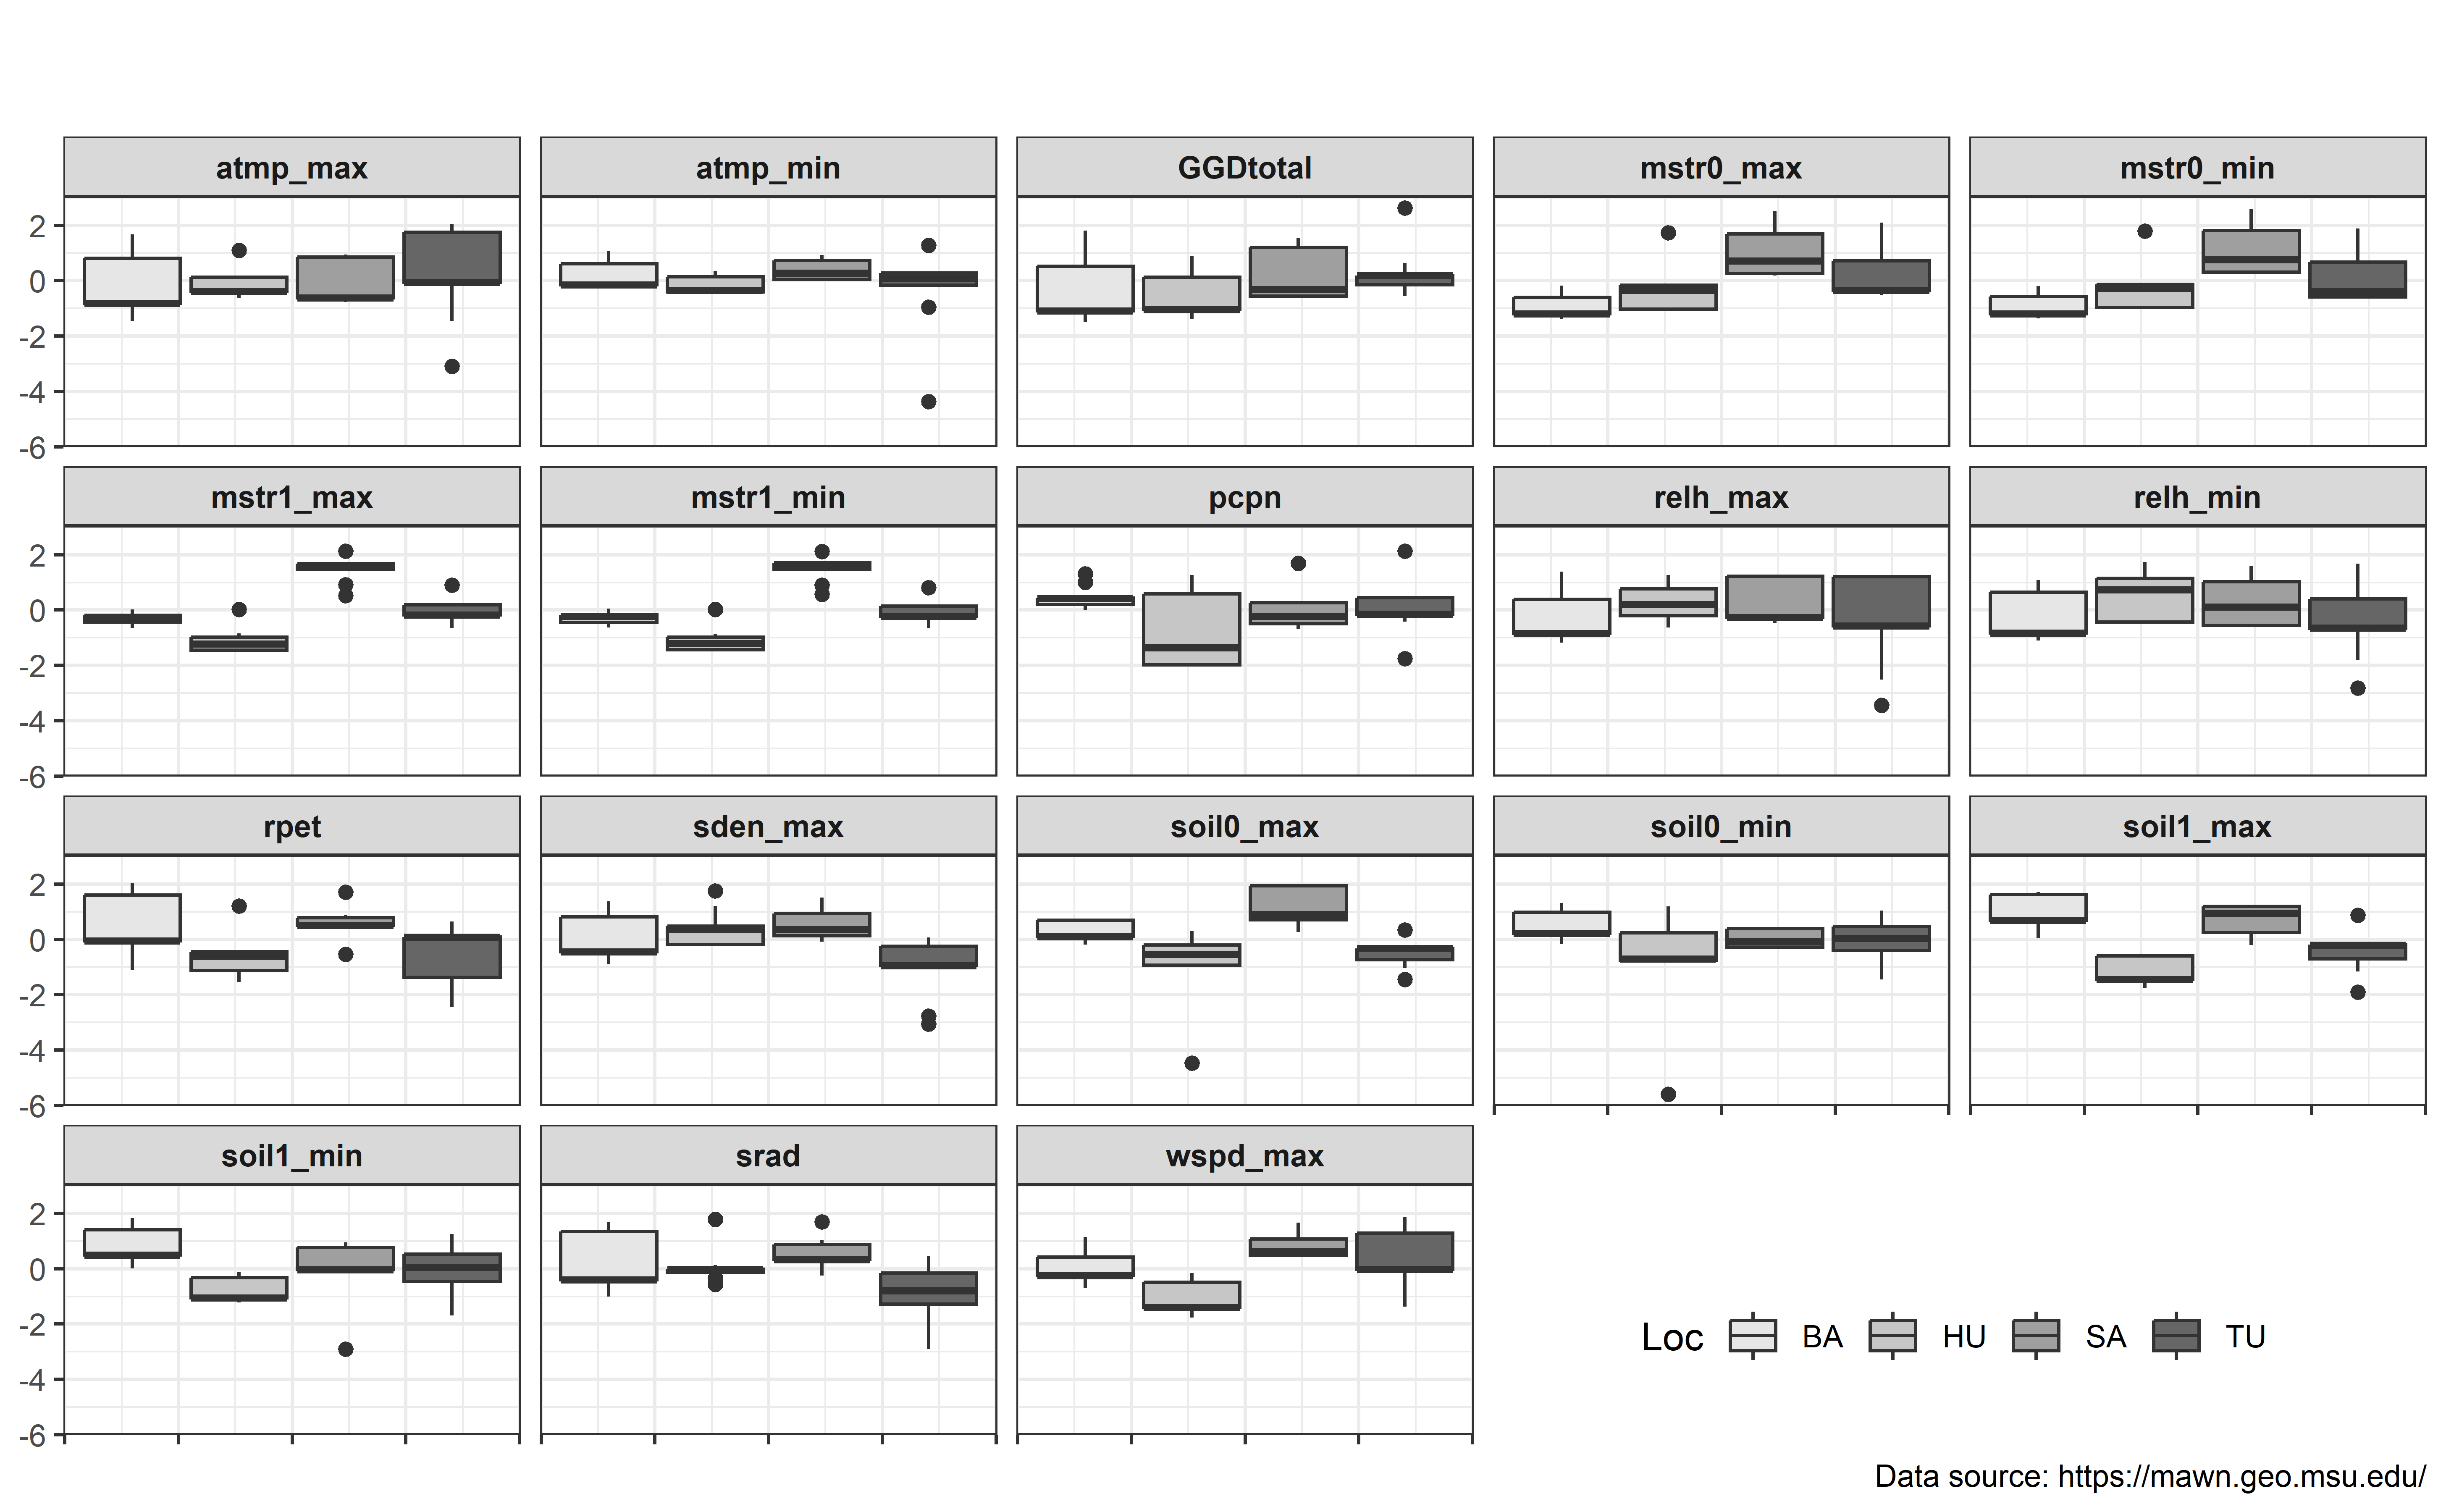
\includegraphics[width=1\linewidth]{figures/weather data1-1} 

}

\caption{Supplemental Figure S1: Box plot distribution from the weather data collected by location from 2017 to 2022 cultivation years. Data were scaled to better plot visualization. Weather data obtained using  daily average value from planting to harvesting.TU: Tuscola, SA: Sanilac, HU: Huron, and BA: Bay locations.}\label{fig:weather data1}
\end{figure}

atmp\_max: Max Air Temperature (1.5m), atmp\_min: Min Air Temperature
(1.5m), mstr0\_max: Max Soil Moisture (0-30cm), mstr0\_min: Min Soil
Moisture (0-30cm), mstr1\_max: Max Soil Moisture (30-60cm), mstr1\_min:
Min Soil Moisture (30-60cm), pcpn: Precipitation, relh\_max: Max
Relative Humidity (1.5m), relh\_min: Min Relative Humidity (1.5m), rpet:
Reference Potential Evapotranspiration, sden\_max: Max Solar Flux,
soil0\_max: Max Soil Temperature (5cm), soil0\_min: Min Soil Temperature
(5cm), soil1\_max: Max Soil Temperature (10cm), soil1\_min: Min Soil
Temperature (10cm), srad: Total Solar Flux, wspd\_max: Max Wind Speed
(3m). GGDtotal: Growing Degree-Day Calculations in Celsius (C) given by:
\((max-min)/2-10\)

\pagebreak

\begin{figure}[H]

{\centering 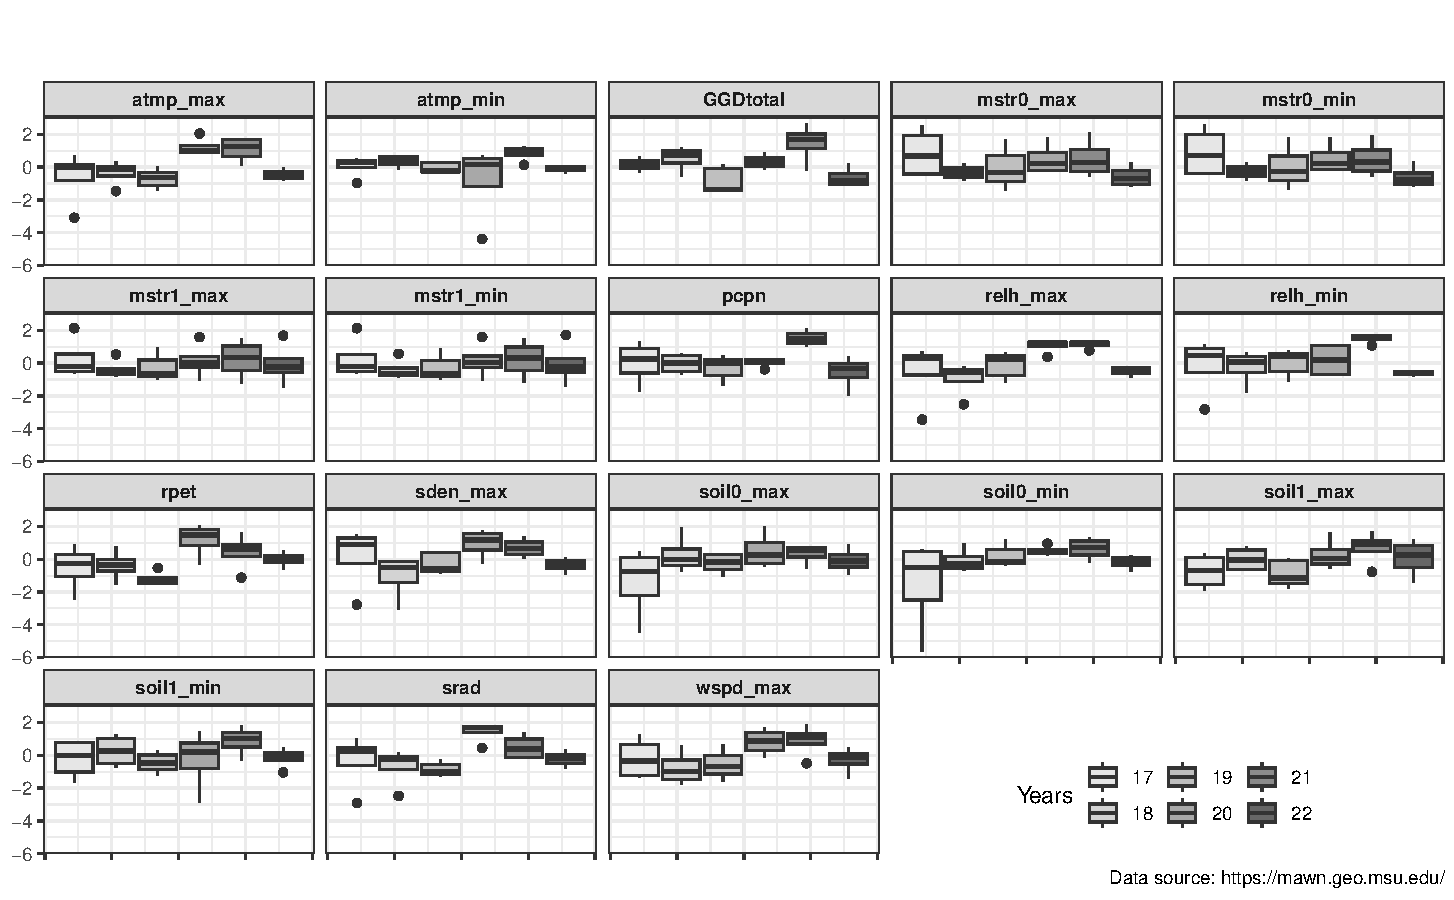
\includegraphics[width=1\linewidth]{figures/weather data2-1} 

}

\caption{Supplemental Figure S2: Box plot distribution from the weather data collected by year from 2017 to 2022 cultivation locations. Data were scaled to better plot visualization. Weather data obtained using  daily average value from planting to harvesting.TU: Tuscola, SA: Sanilac, HU: Huron, and BA: Bay locations.}\label{fig:weather data2}
\end{figure}

atmp\_max: Max Air Temperature (1.5m), atmp\_min: Min Air Temperature
(1.5m), mstr0\_max: Max Soil Moisture (0-30cm), mstr0\_min: Min Soil
Moisture (0-30cm), mstr1\_max: Max Soil Moisture (30-60cm), mstr1\_min:
Min Soil Moisture (30-60cm), pcpn: Precipitation, relh\_max: Max
Relative Humidity (1.5m), relh\_min: Min Relative Humidity (1.5m), rpet:
Reference Potential Evapotranspiration, sden\_max: Max Solar Flux,
soil0\_max: Max Soil Temperature (5cm), soil0\_min: Min Soil Temperature
(5cm), soil1\_max: Max Soil Temperature (10cm), soil1\_min: Min Soil
Temperature (10cm), srad: Total Solar Flux, wspd\_max: Max Wind Speed
(3m). GGDtotal: Growing Degree-Day Calculations in Celsius (C) given by:
\((max-min)/2-10\)

\pagebreak

\begin{figure}[H]

{\centering 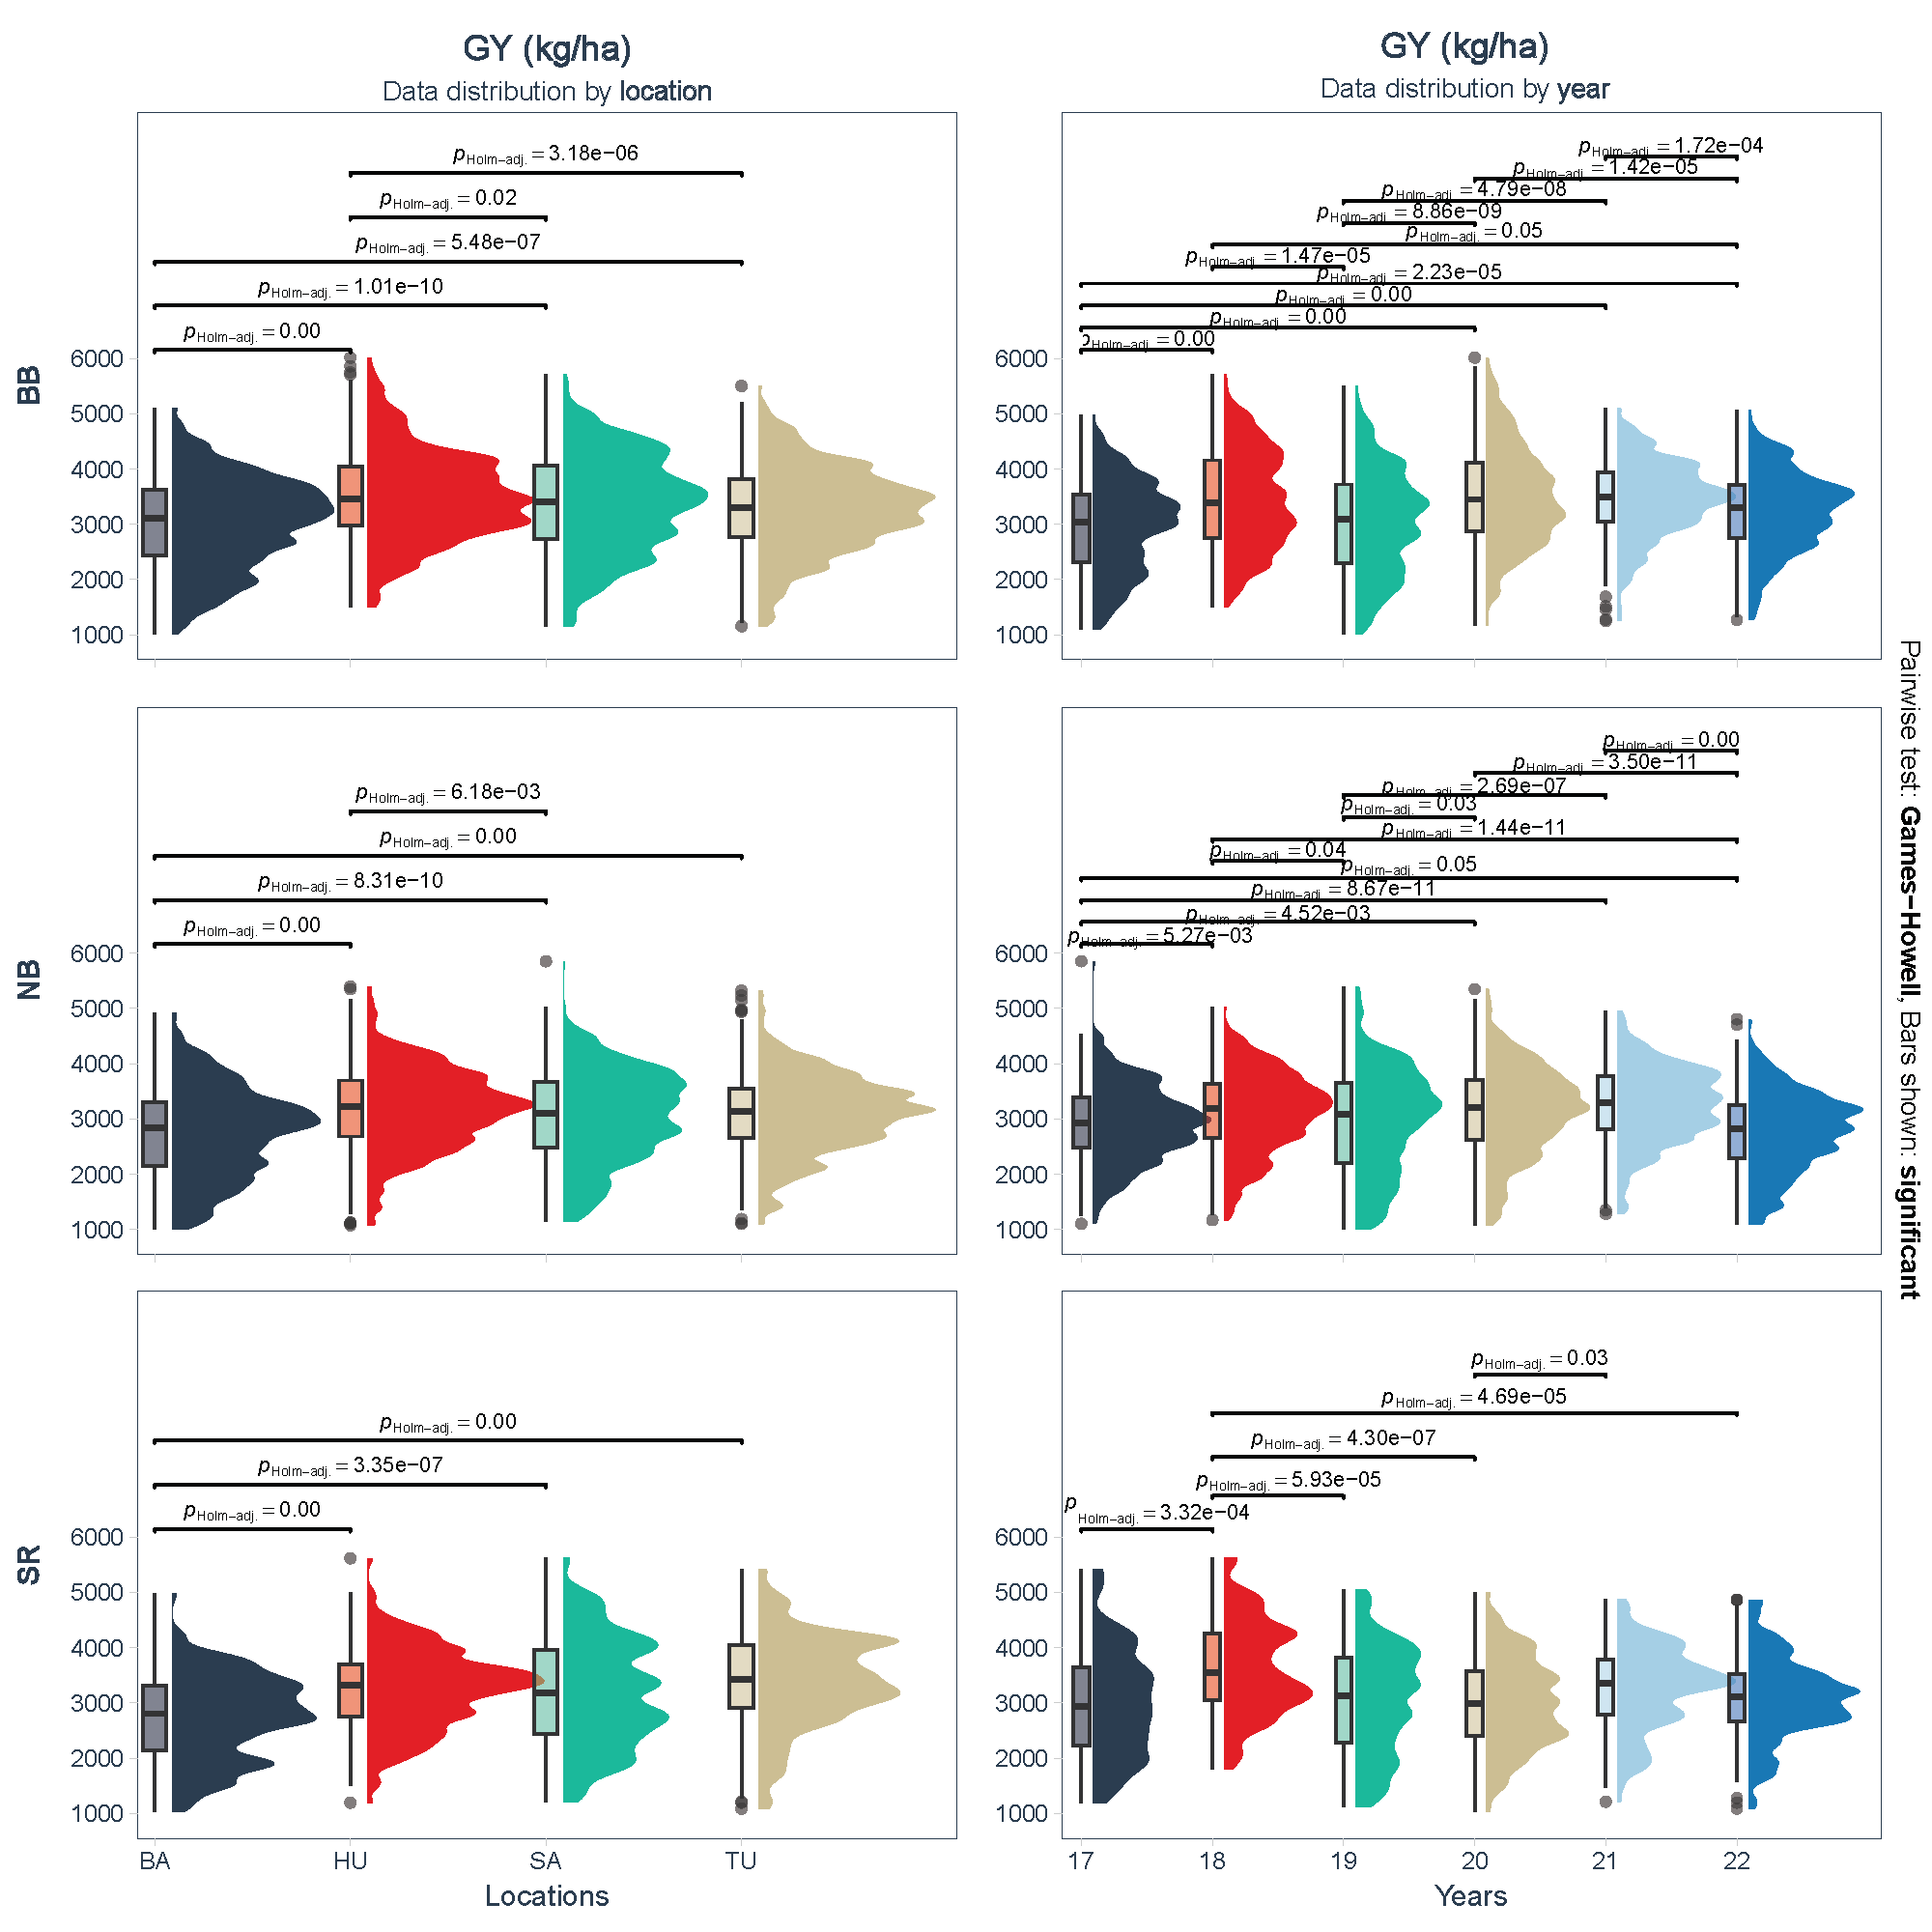
\includegraphics[width=1\linewidth]{main-figures/Plot_dist_GY} 

}

\caption{Supplemental Figure S3: Combination of box and density plots for between subjects comparisons by locations (left) and year (right) of grain yield (GY in Kg/ha) for black (BB), Navy (NB) and Small Red (SR) beans. BA: Bay, HU: Huron, SA:Sanilac, TU: Tuscola locations.}\label{fig:plot_ggstatsplot1}
\end{figure}

\pagebreak

\begin{figure}[H]

{\centering 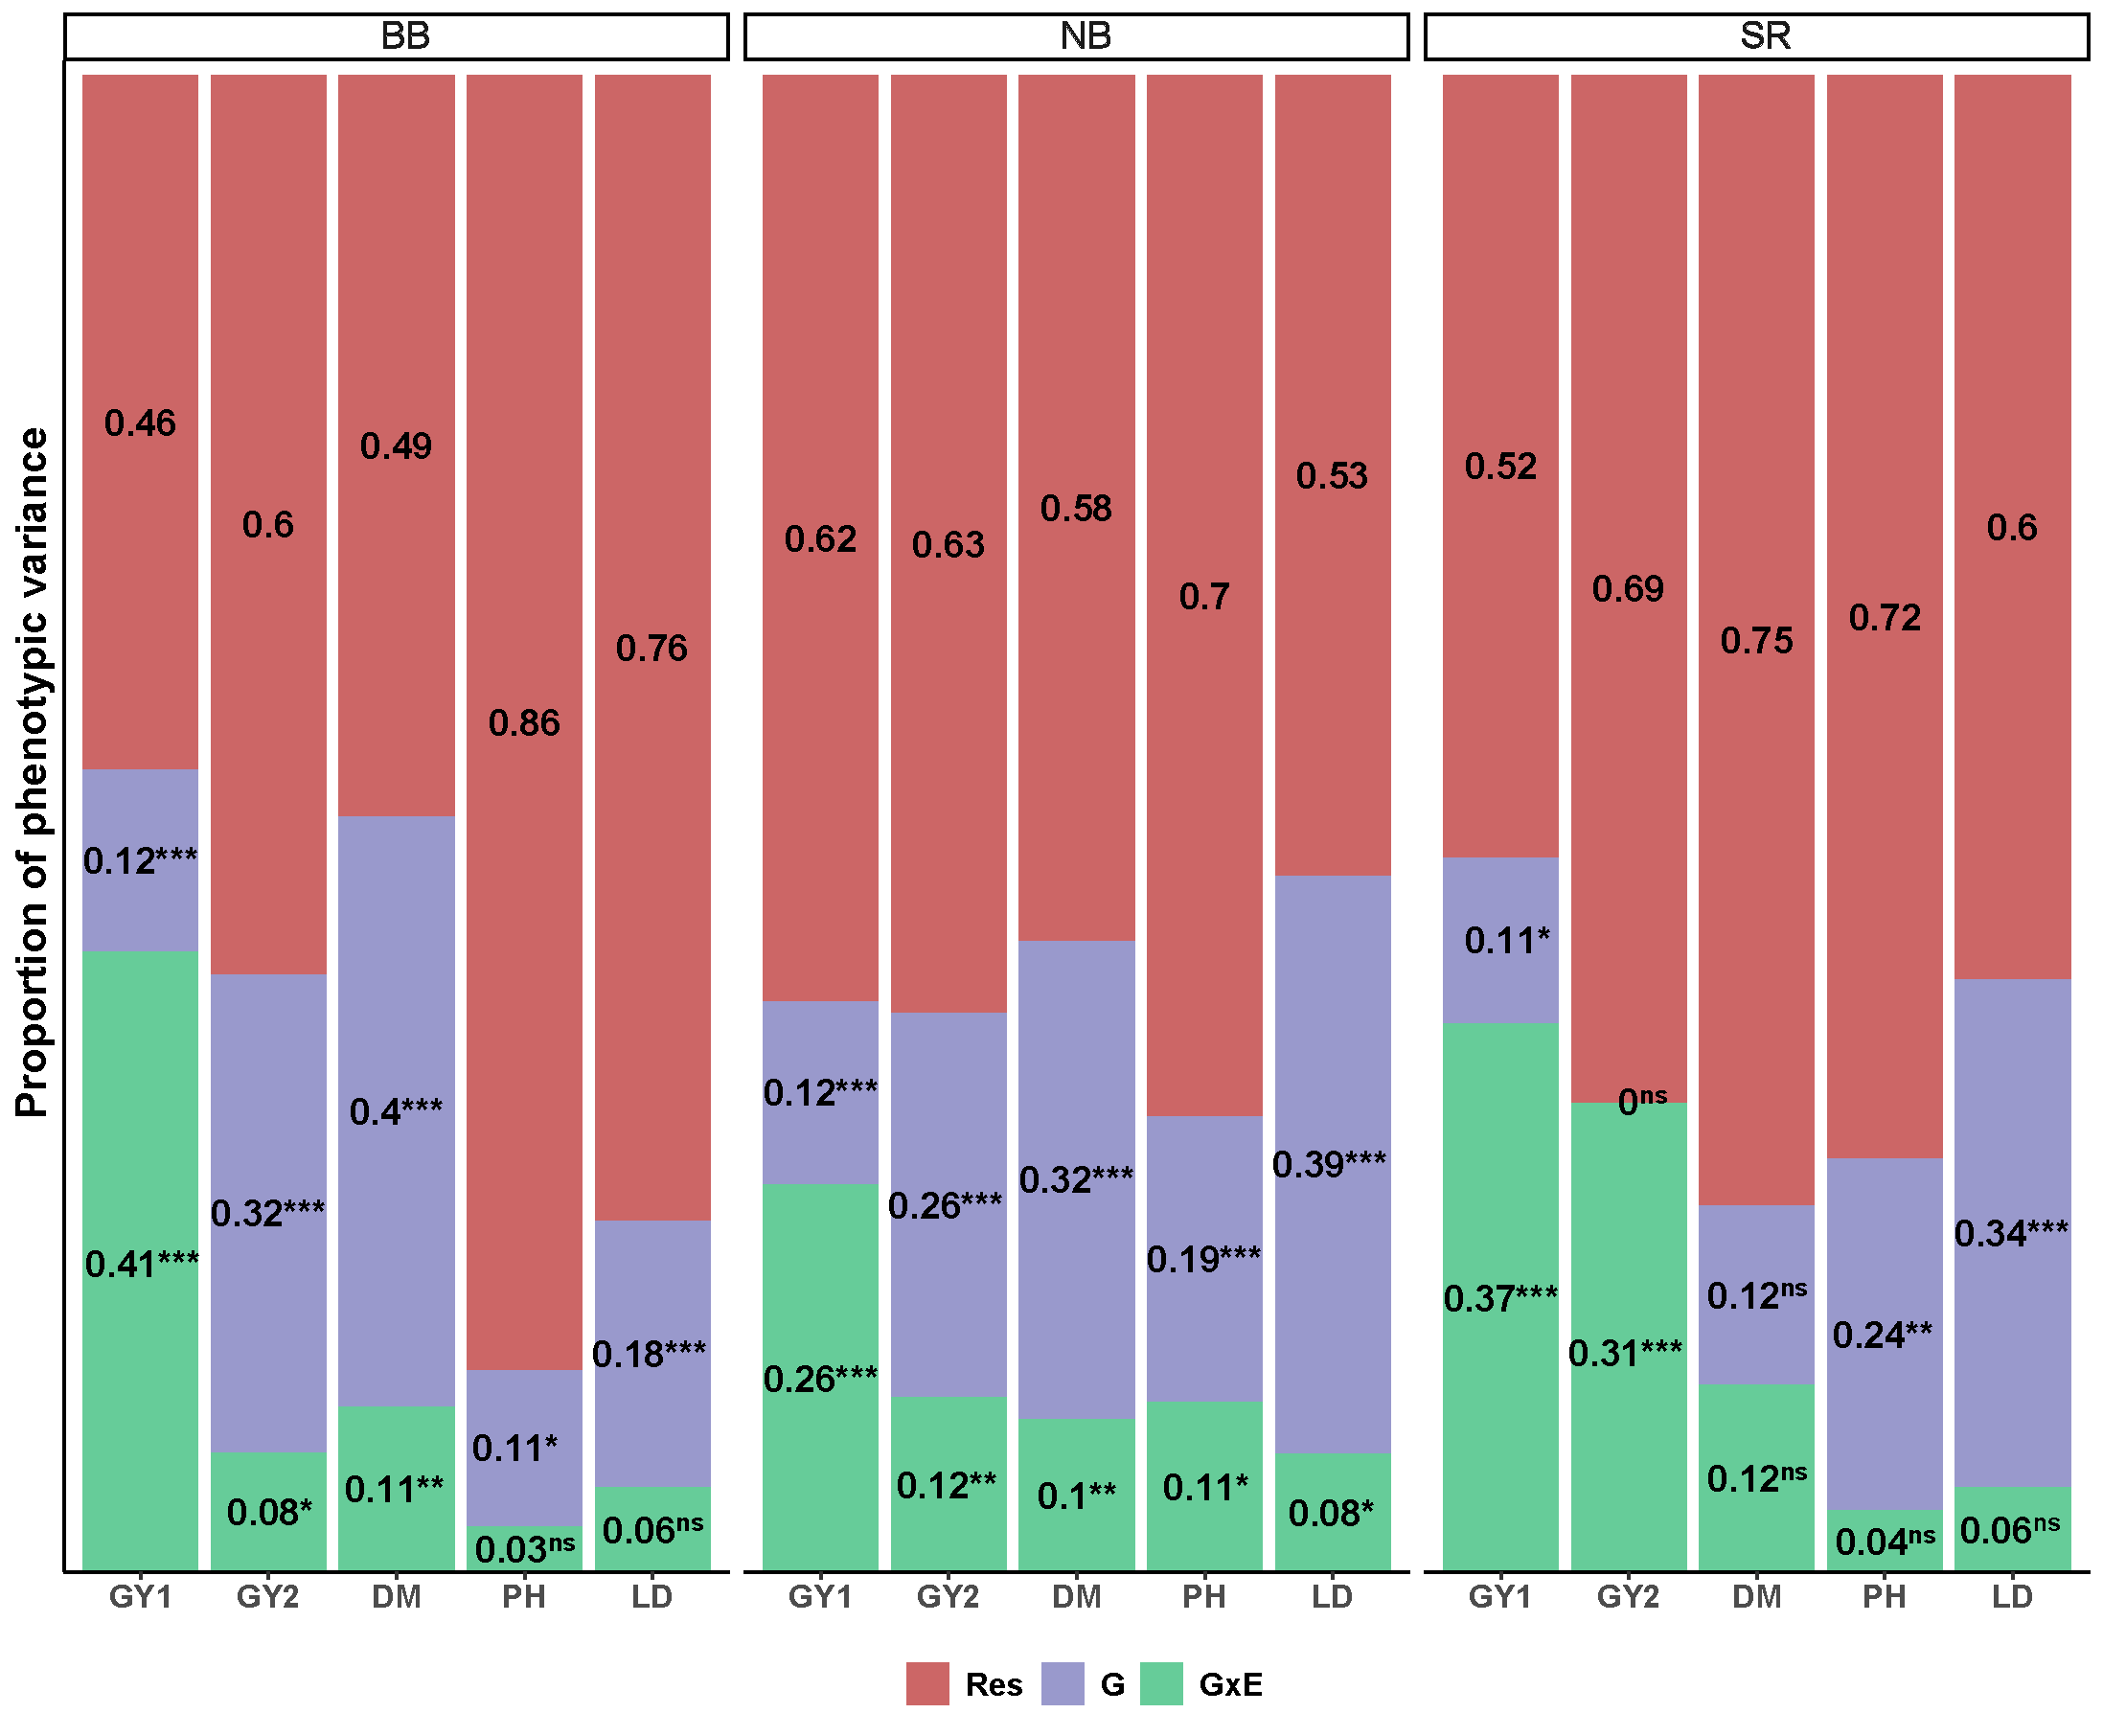
\includegraphics[width=1\linewidth]{main-figures/Rplot_VarCompFinal} 

}

\caption{Supplemental Figure S4:Proportion of the phenotypic variance for 71 Black (BB), 72 Navy (NB), and 21 Red (SR) beans for grain yield in Kg/ha (GY: 2017 - 2022; GY2: only 2021) days to maturity (DM, days), plant height (PH, cm) and lodging (LD,scale) traits evaluated in the study. * Significant at P < 0.05. ** Significant at P < 0.01. *** Significant at P < 0.001. ns, nonsignificant.}\label{fig:selected geno bb}
\end{figure}

\pagebreak

\begin{figure}[H]

{\centering 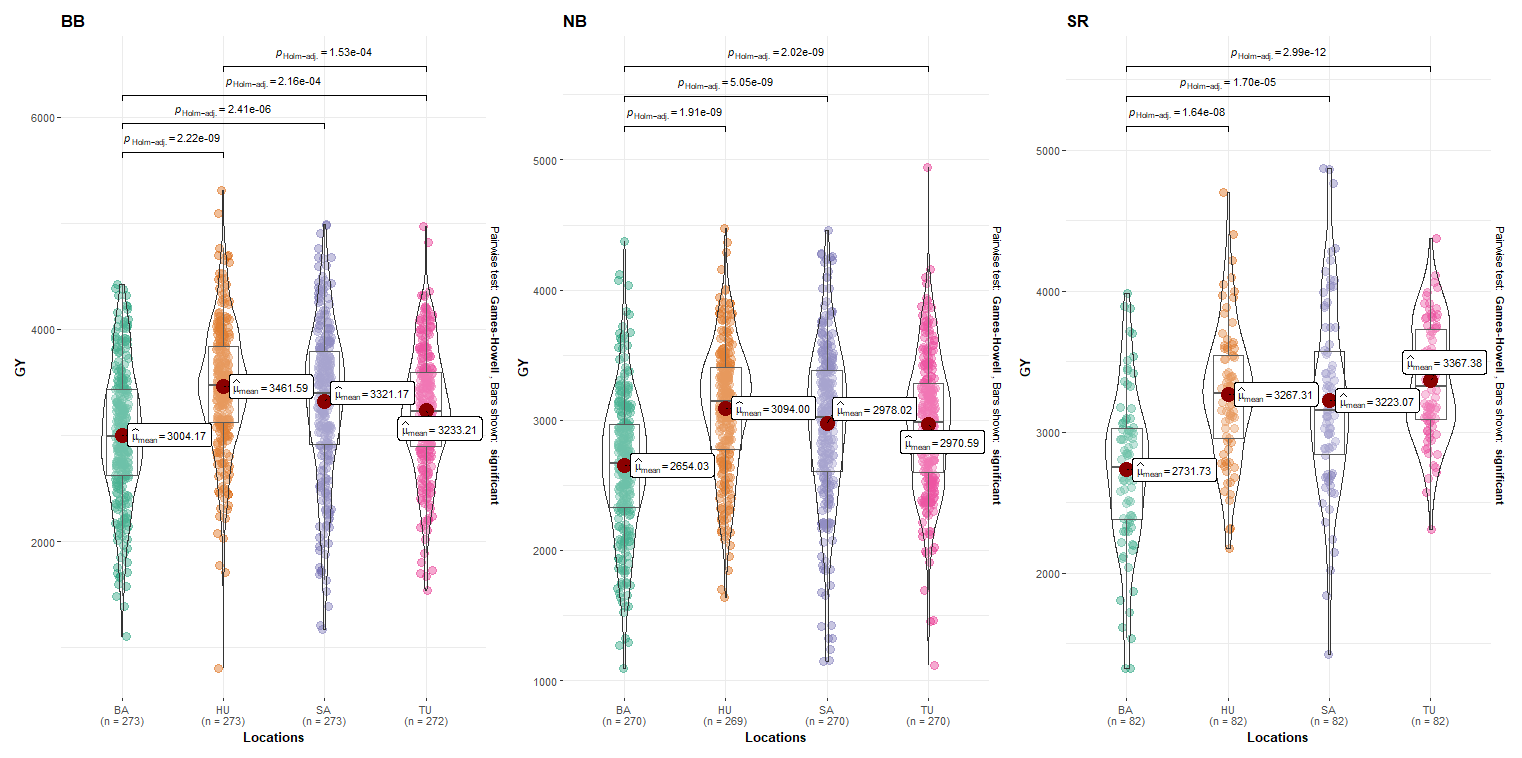
\includegraphics[width=1\linewidth]{main-figures/Boxviolin_blues} 

}

\caption{Supplemental Figure S5: Combination of box and violin plots along with jittered data points and grand mean values for between subjects comparisons by locations of grain yield (GY) for black (BB), Navy (NB) and Small Red (SR) beans. Pairwise Games-Howell test used. Comparisons showing only significant values. BA: Bay, HU: Huron, SA: Sanilac, TU: Tuscola. Pairwise Games-Howell test used. Comparisons showing only significant between the pairs of environments.}\label{fig:plot_ggstatsplot_met_fig}
\end{figure}

\pagebreak

\begin{figure}[H]

{\centering 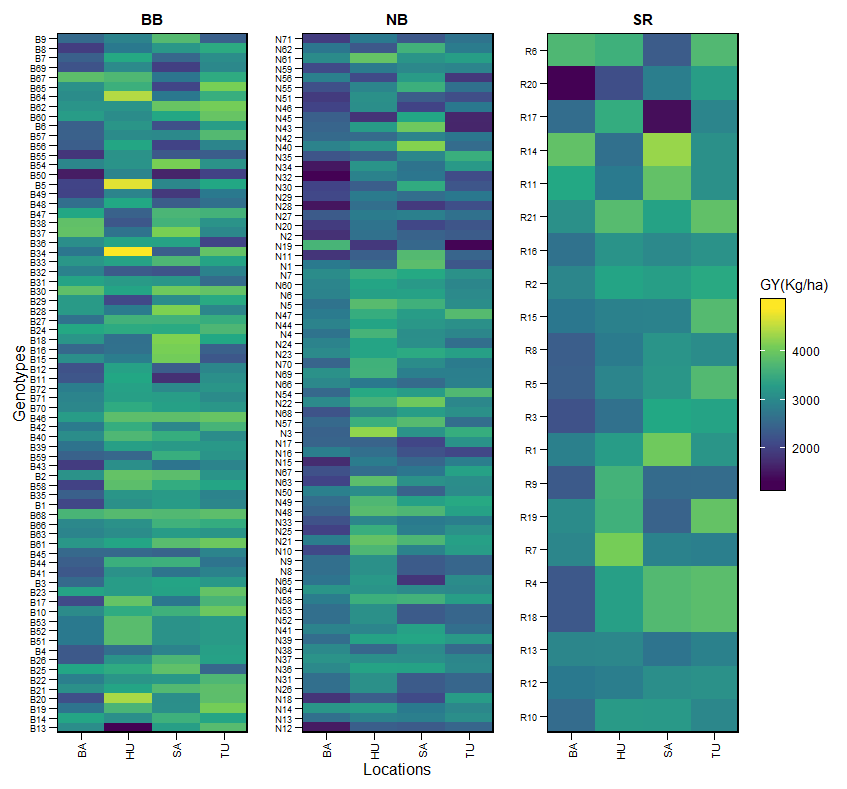
\includegraphics[width=1\linewidth]{main-figures/BLUES_means} 

}

\caption{Supplemental Figure S6: Genotype’s performance across the environments for Black (BB), Navy (NB), and Small Red (SR) beans using the estimated means (BLUEs) values. BA: Bay, HU: Huron, SA:Sanilac, TU: Tuscola locations}\label{fig:plot_ggstatsplot2}
\end{figure}

\pagebreak

\begin{figure}[H]

{\centering 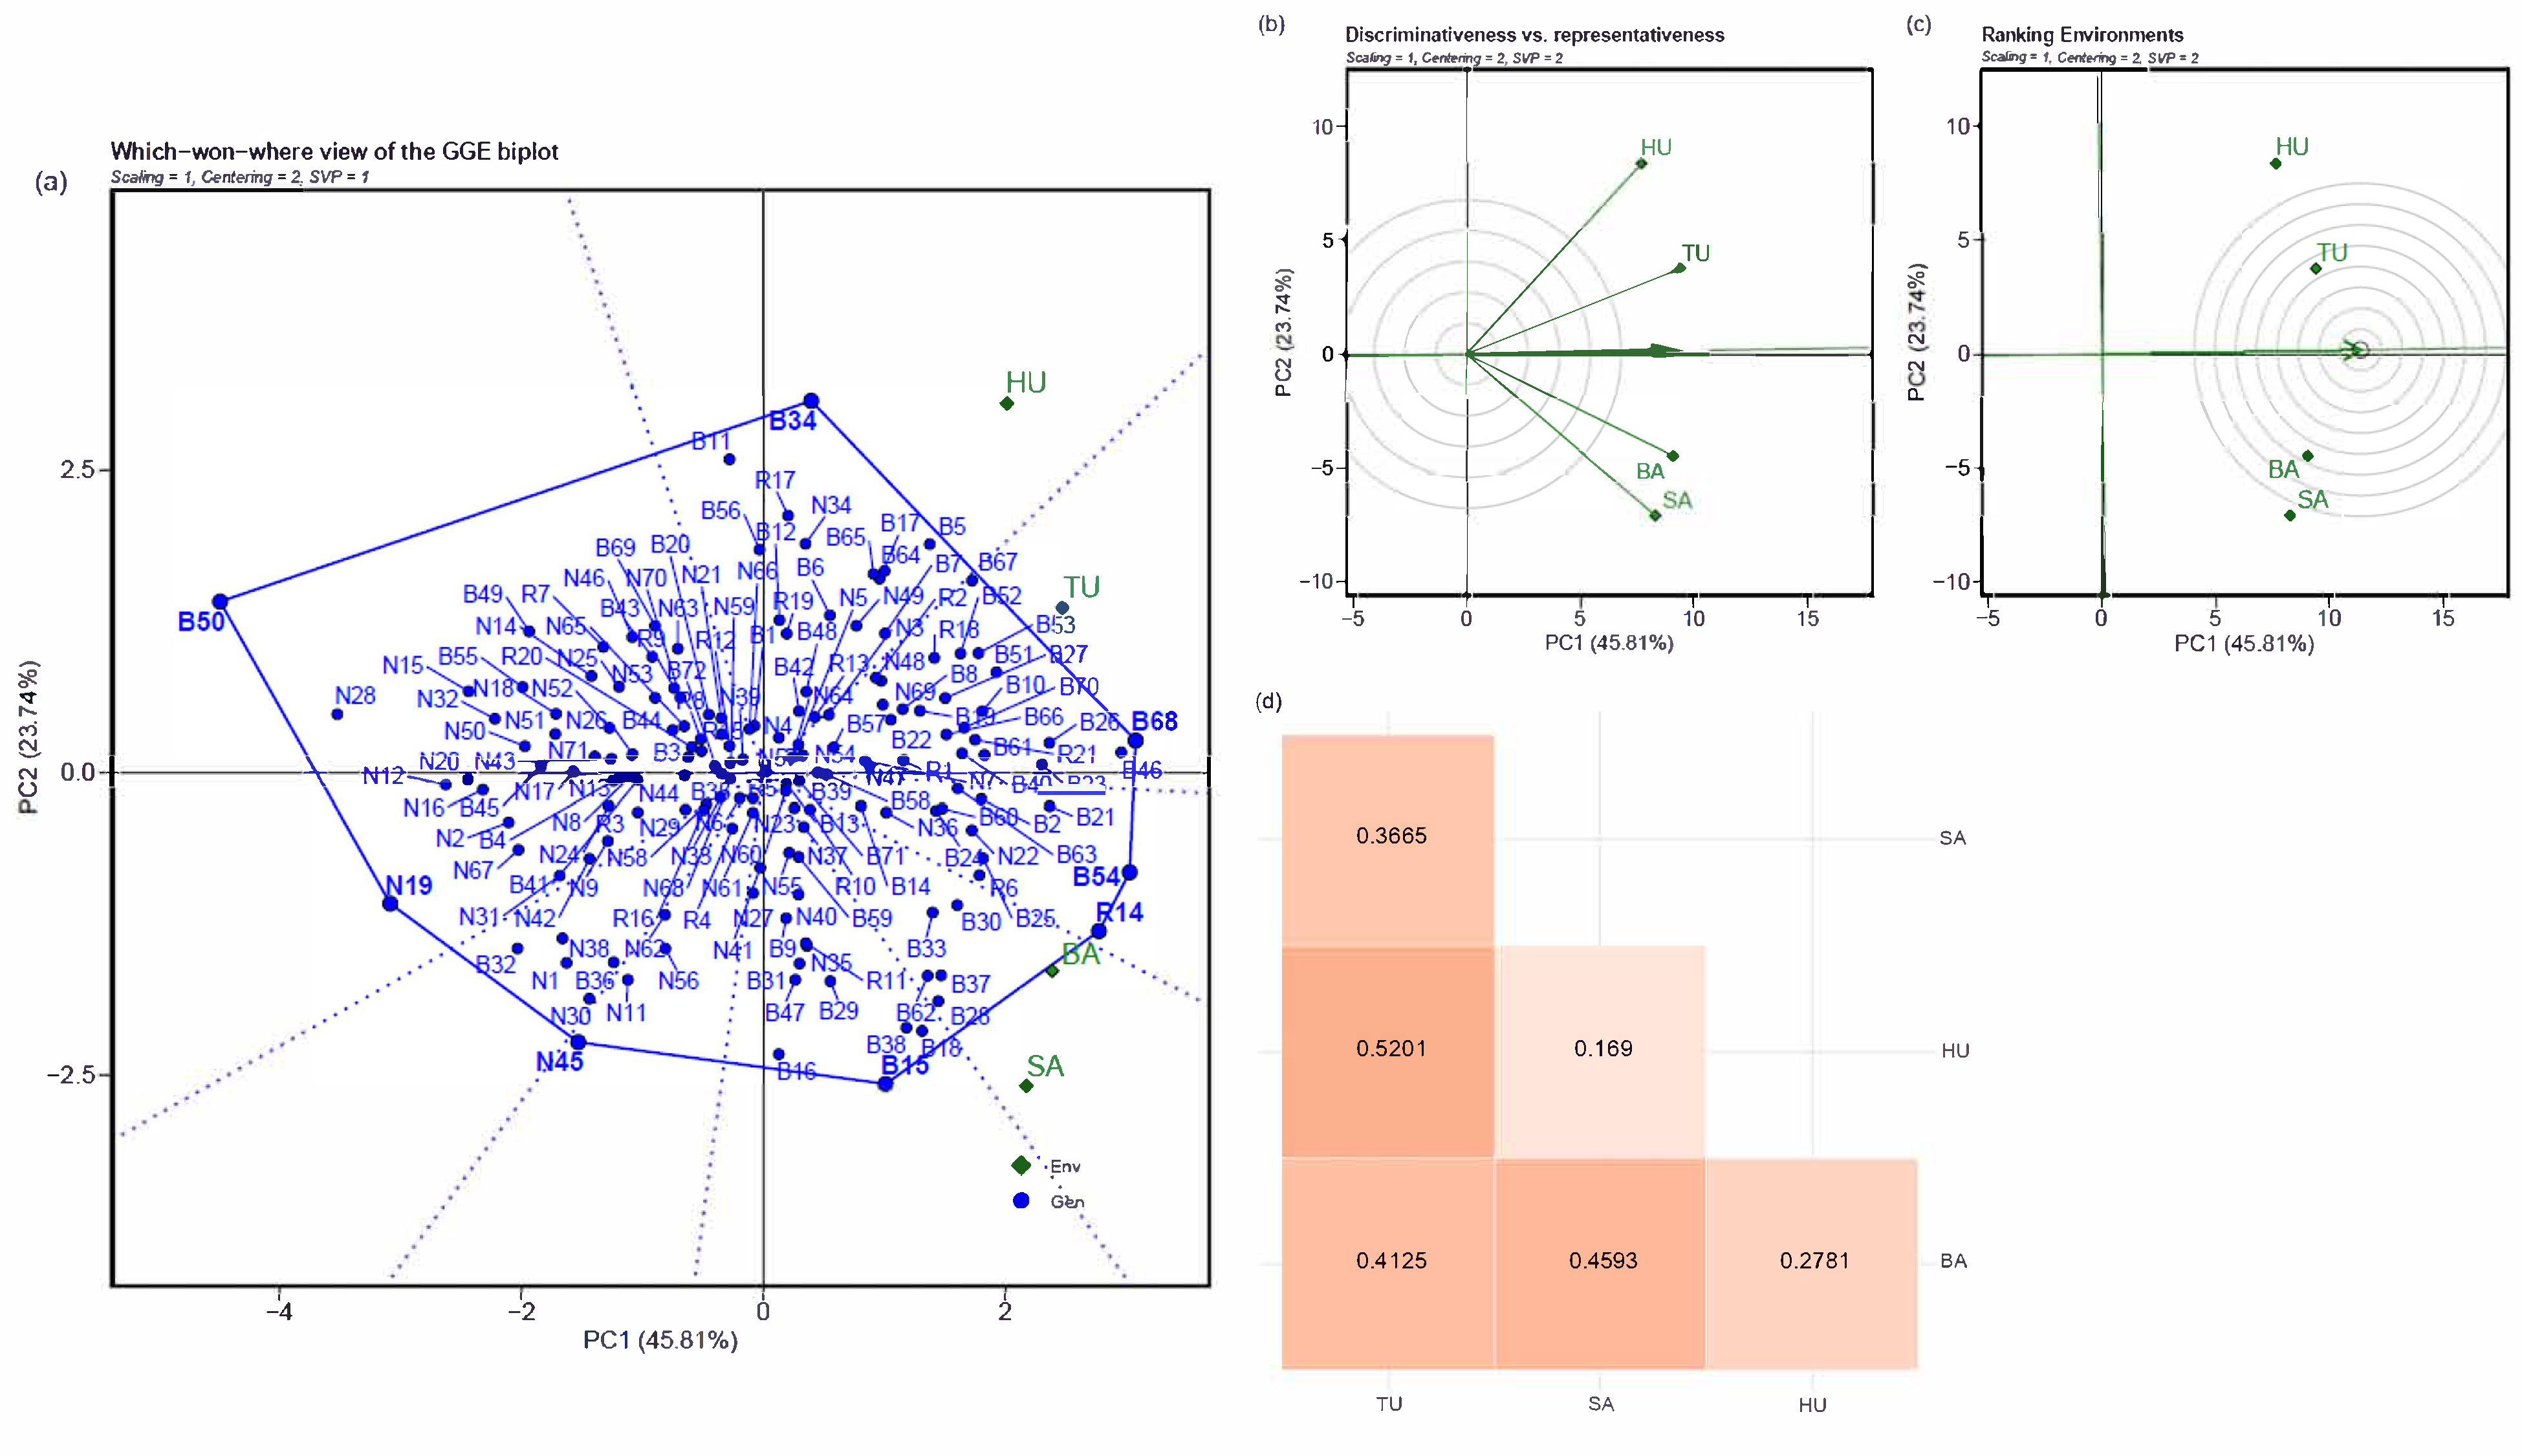
\includegraphics[width=1\linewidth]{main-figures/S12_allMKT2} 

}

\caption{Supplemental Figure S7: Genotype x environment interaction characterization of all beans market classes combined dataset from 2017 to 2022. The left panel (a) shows a GGE biplot using the adjusted grain yield (GY) phenotypic means for each location averaged across years. Mega-environments (MEs, in the divided sector by the perpendicular lines to the sides of the polygon) were built using the winning genotypes from the GGE biplot. The right top panel (b) shows the discriminativeness and representativeness among environments and in relation to (c) the ideal environment. The right bottom panel (d) shows the GEI correlation among locations. PC, principal component; BA, Bay; TU, Tuscola; HU, Huron; SA, Sanilac.}\label{fig:S7 ok}
\end{figure}

\pagebreak

\begin{figure}[H]

{\centering 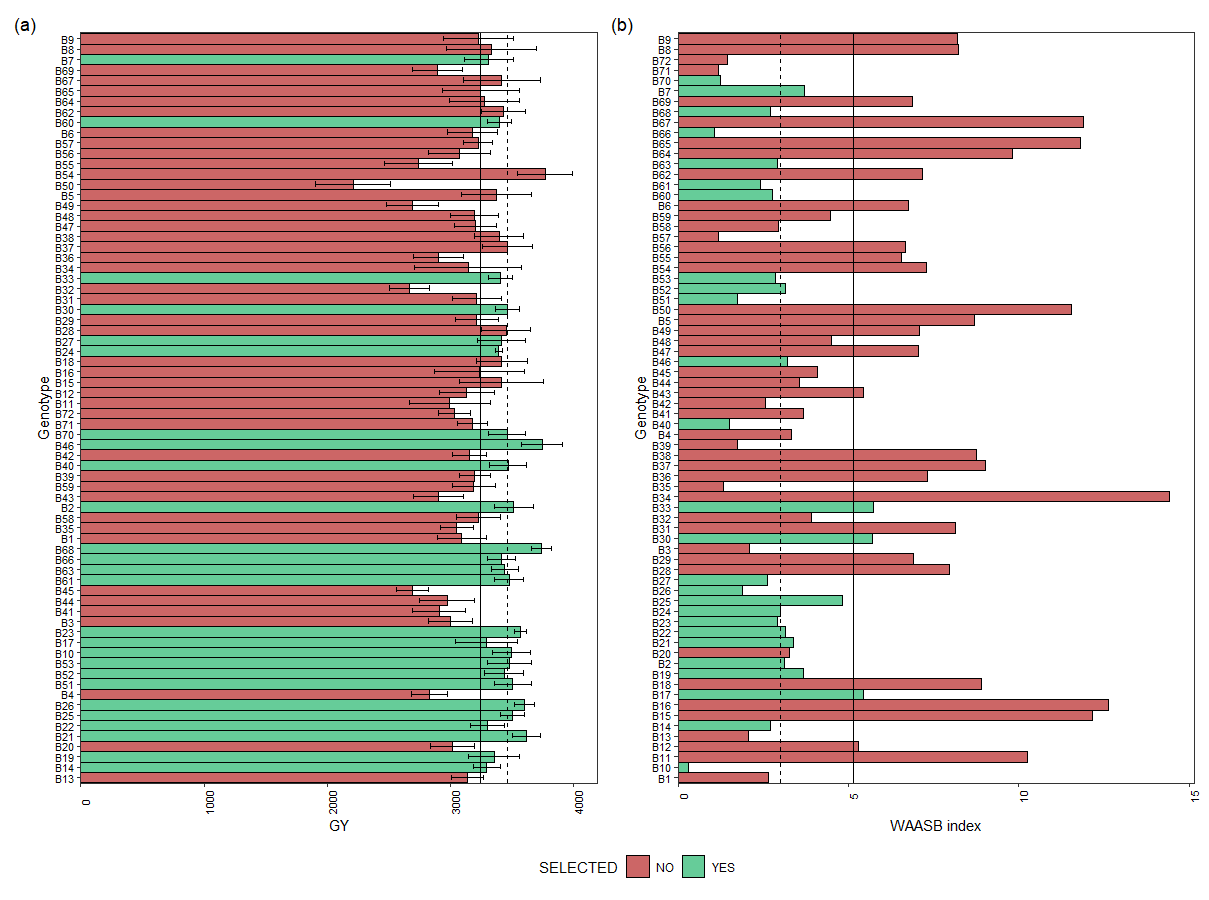
\includegraphics[width=1\linewidth]{main-figures/Sel_GY_BB} 

}

\caption{Supplemental Figure S8: Mean performance (a) and stability (b) for grain yield (GY) of 72 black beans genotypes. The vertical dashed and solid lines show, respectively, the  mean of the selected genotype and the overall mean for both mean performance and WAASB index.}\label{fig:selected geno bb2}
\end{figure}

\pagebreak

\begin{figure}[H]

{\centering 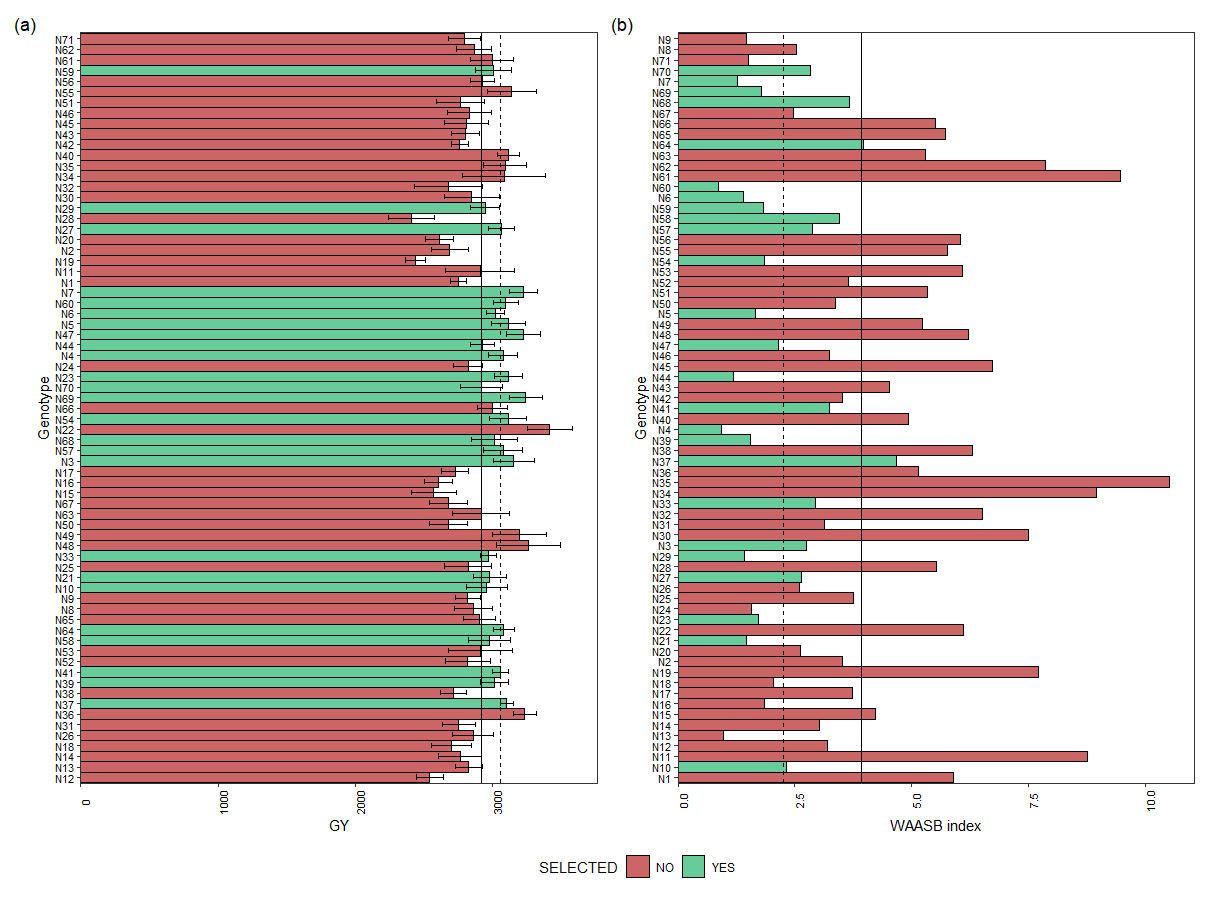
\includegraphics[width=1\linewidth]{main-figures/Sel_GY_NB} 

}

\caption{Supplemental Figure S9: Mean performance (a) and stability (b) for grain yield (GY) of 71 navy beans genotypes. The vertical dashed and solid lines show, respectively, the  mean of the selected genotype and the overall mean for both mean performance and WAASB index.}\label{fig:selected geno nb}
\end{figure}

\pagebreak

\begin{figure}[H]

{\centering 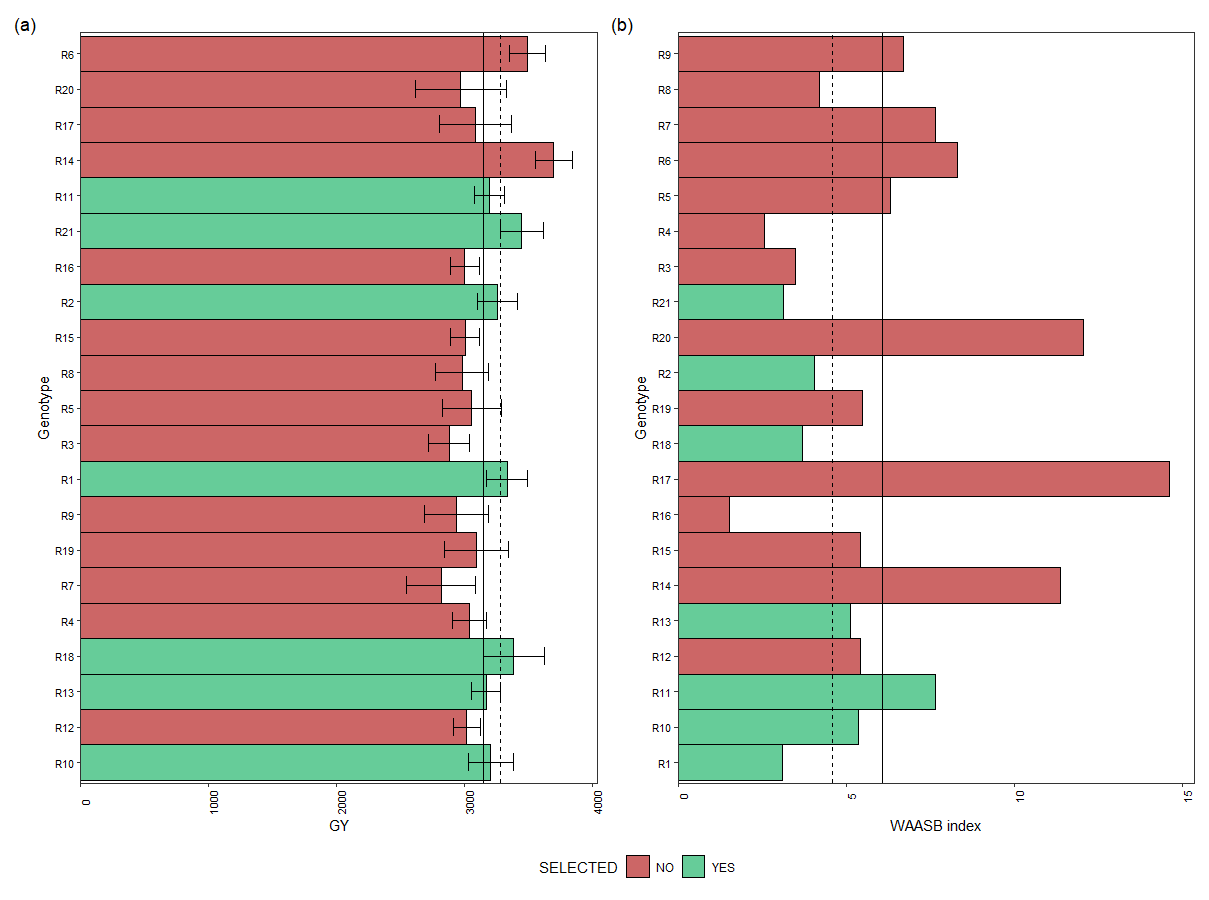
\includegraphics[width=1\linewidth]{main-figures/Sel_GY_SR} 

}

\caption{Supplemental Figure S10: Mean performance (a) and stability (b) for grain yield (GY) of 21 red beans genotypes. The vertical dashed and solid lines show, respectively, the  mean of the selected genotype and the overall mean for both mean performance and WAASB index.}\label{fig:selected geno sr}
\end{figure}

\pagebreak

\begin{figure}[H]

{\centering 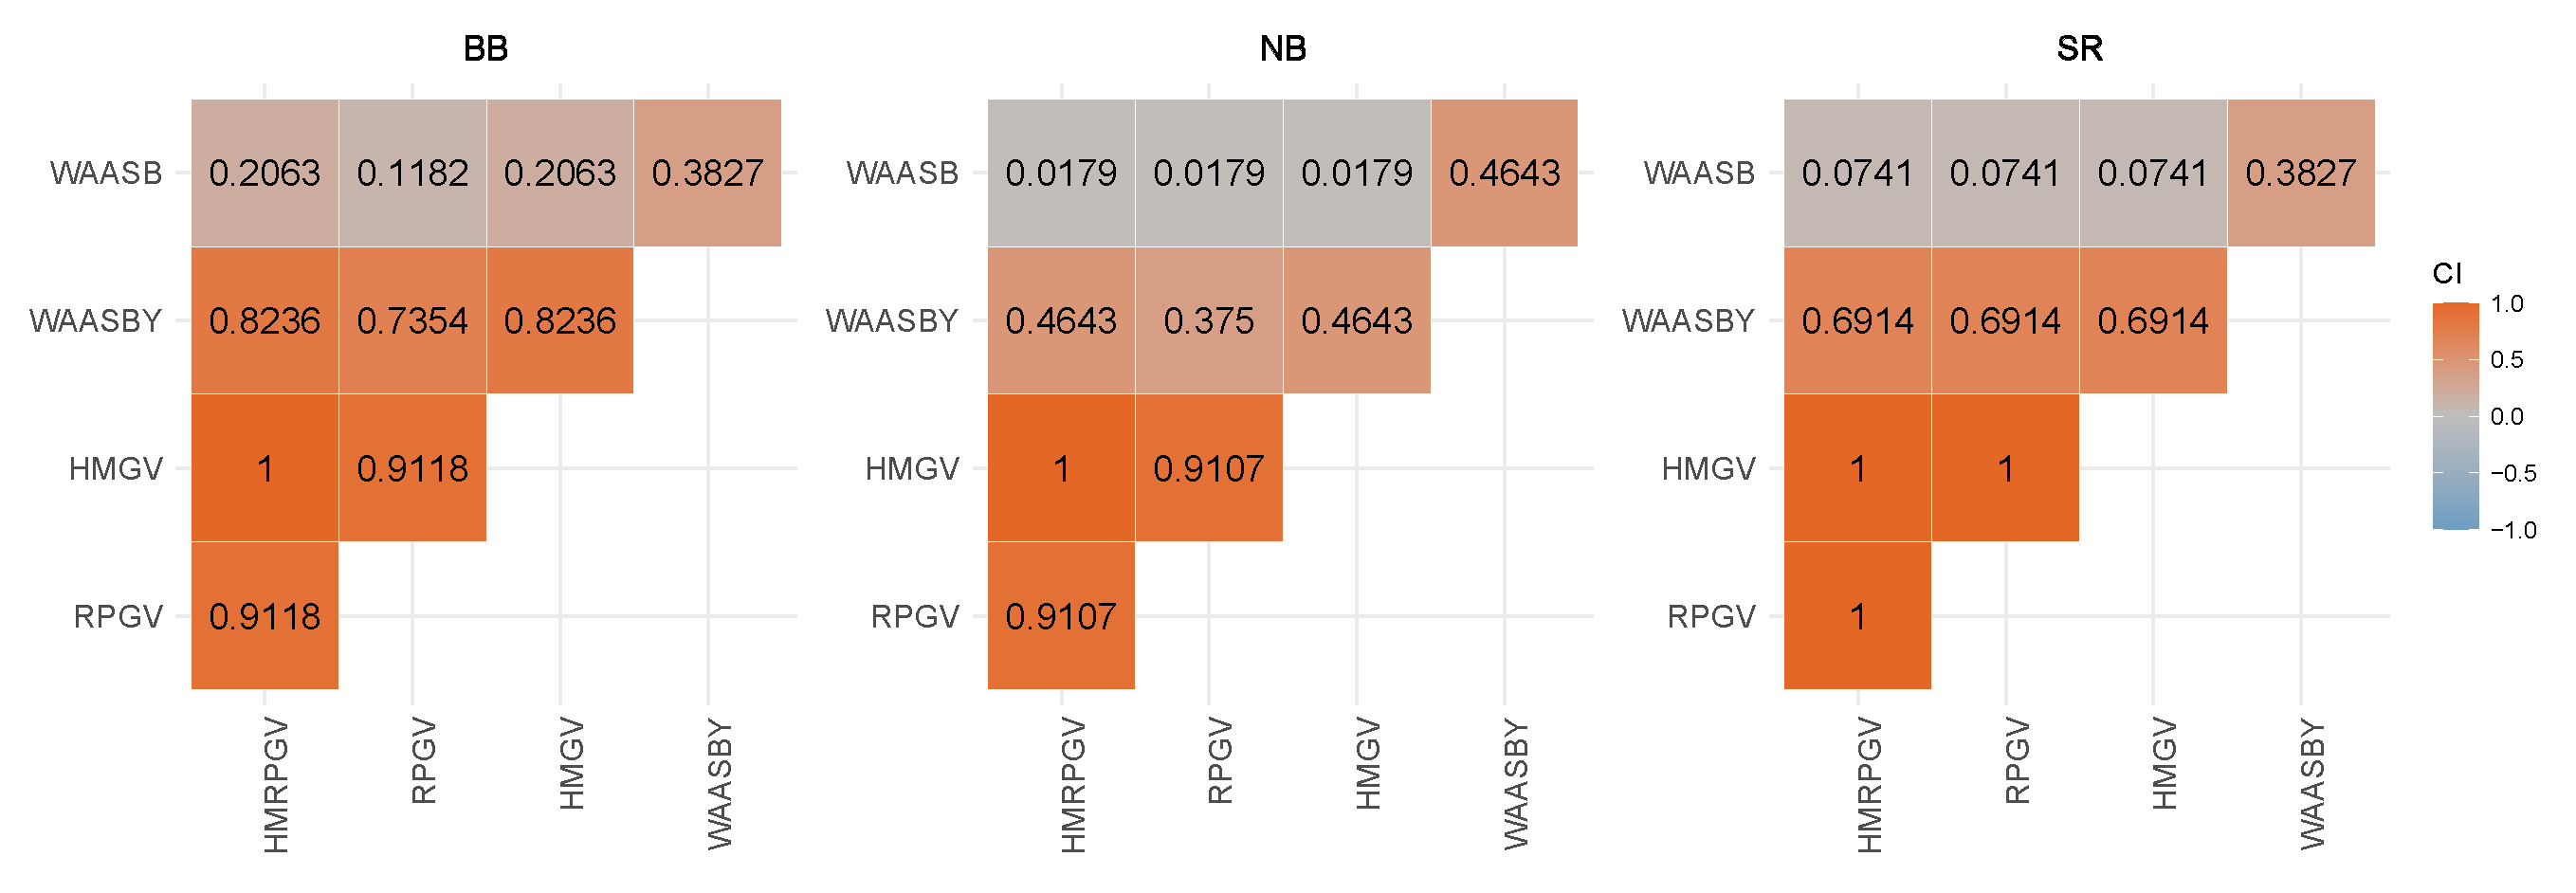
\includegraphics[width=1\linewidth]{main-figures/CI_blups} 

}

\caption{Supplemental Figure S11: BLUP-based stability indexes coincidence index (CI) using selection intensity of 20 top genotypes. BB, black; NB, navy; SR, red beans.}\label{fig:blups CI2}
\end{figure}

\pagebreak

\begin{figure}[H]

{\centering 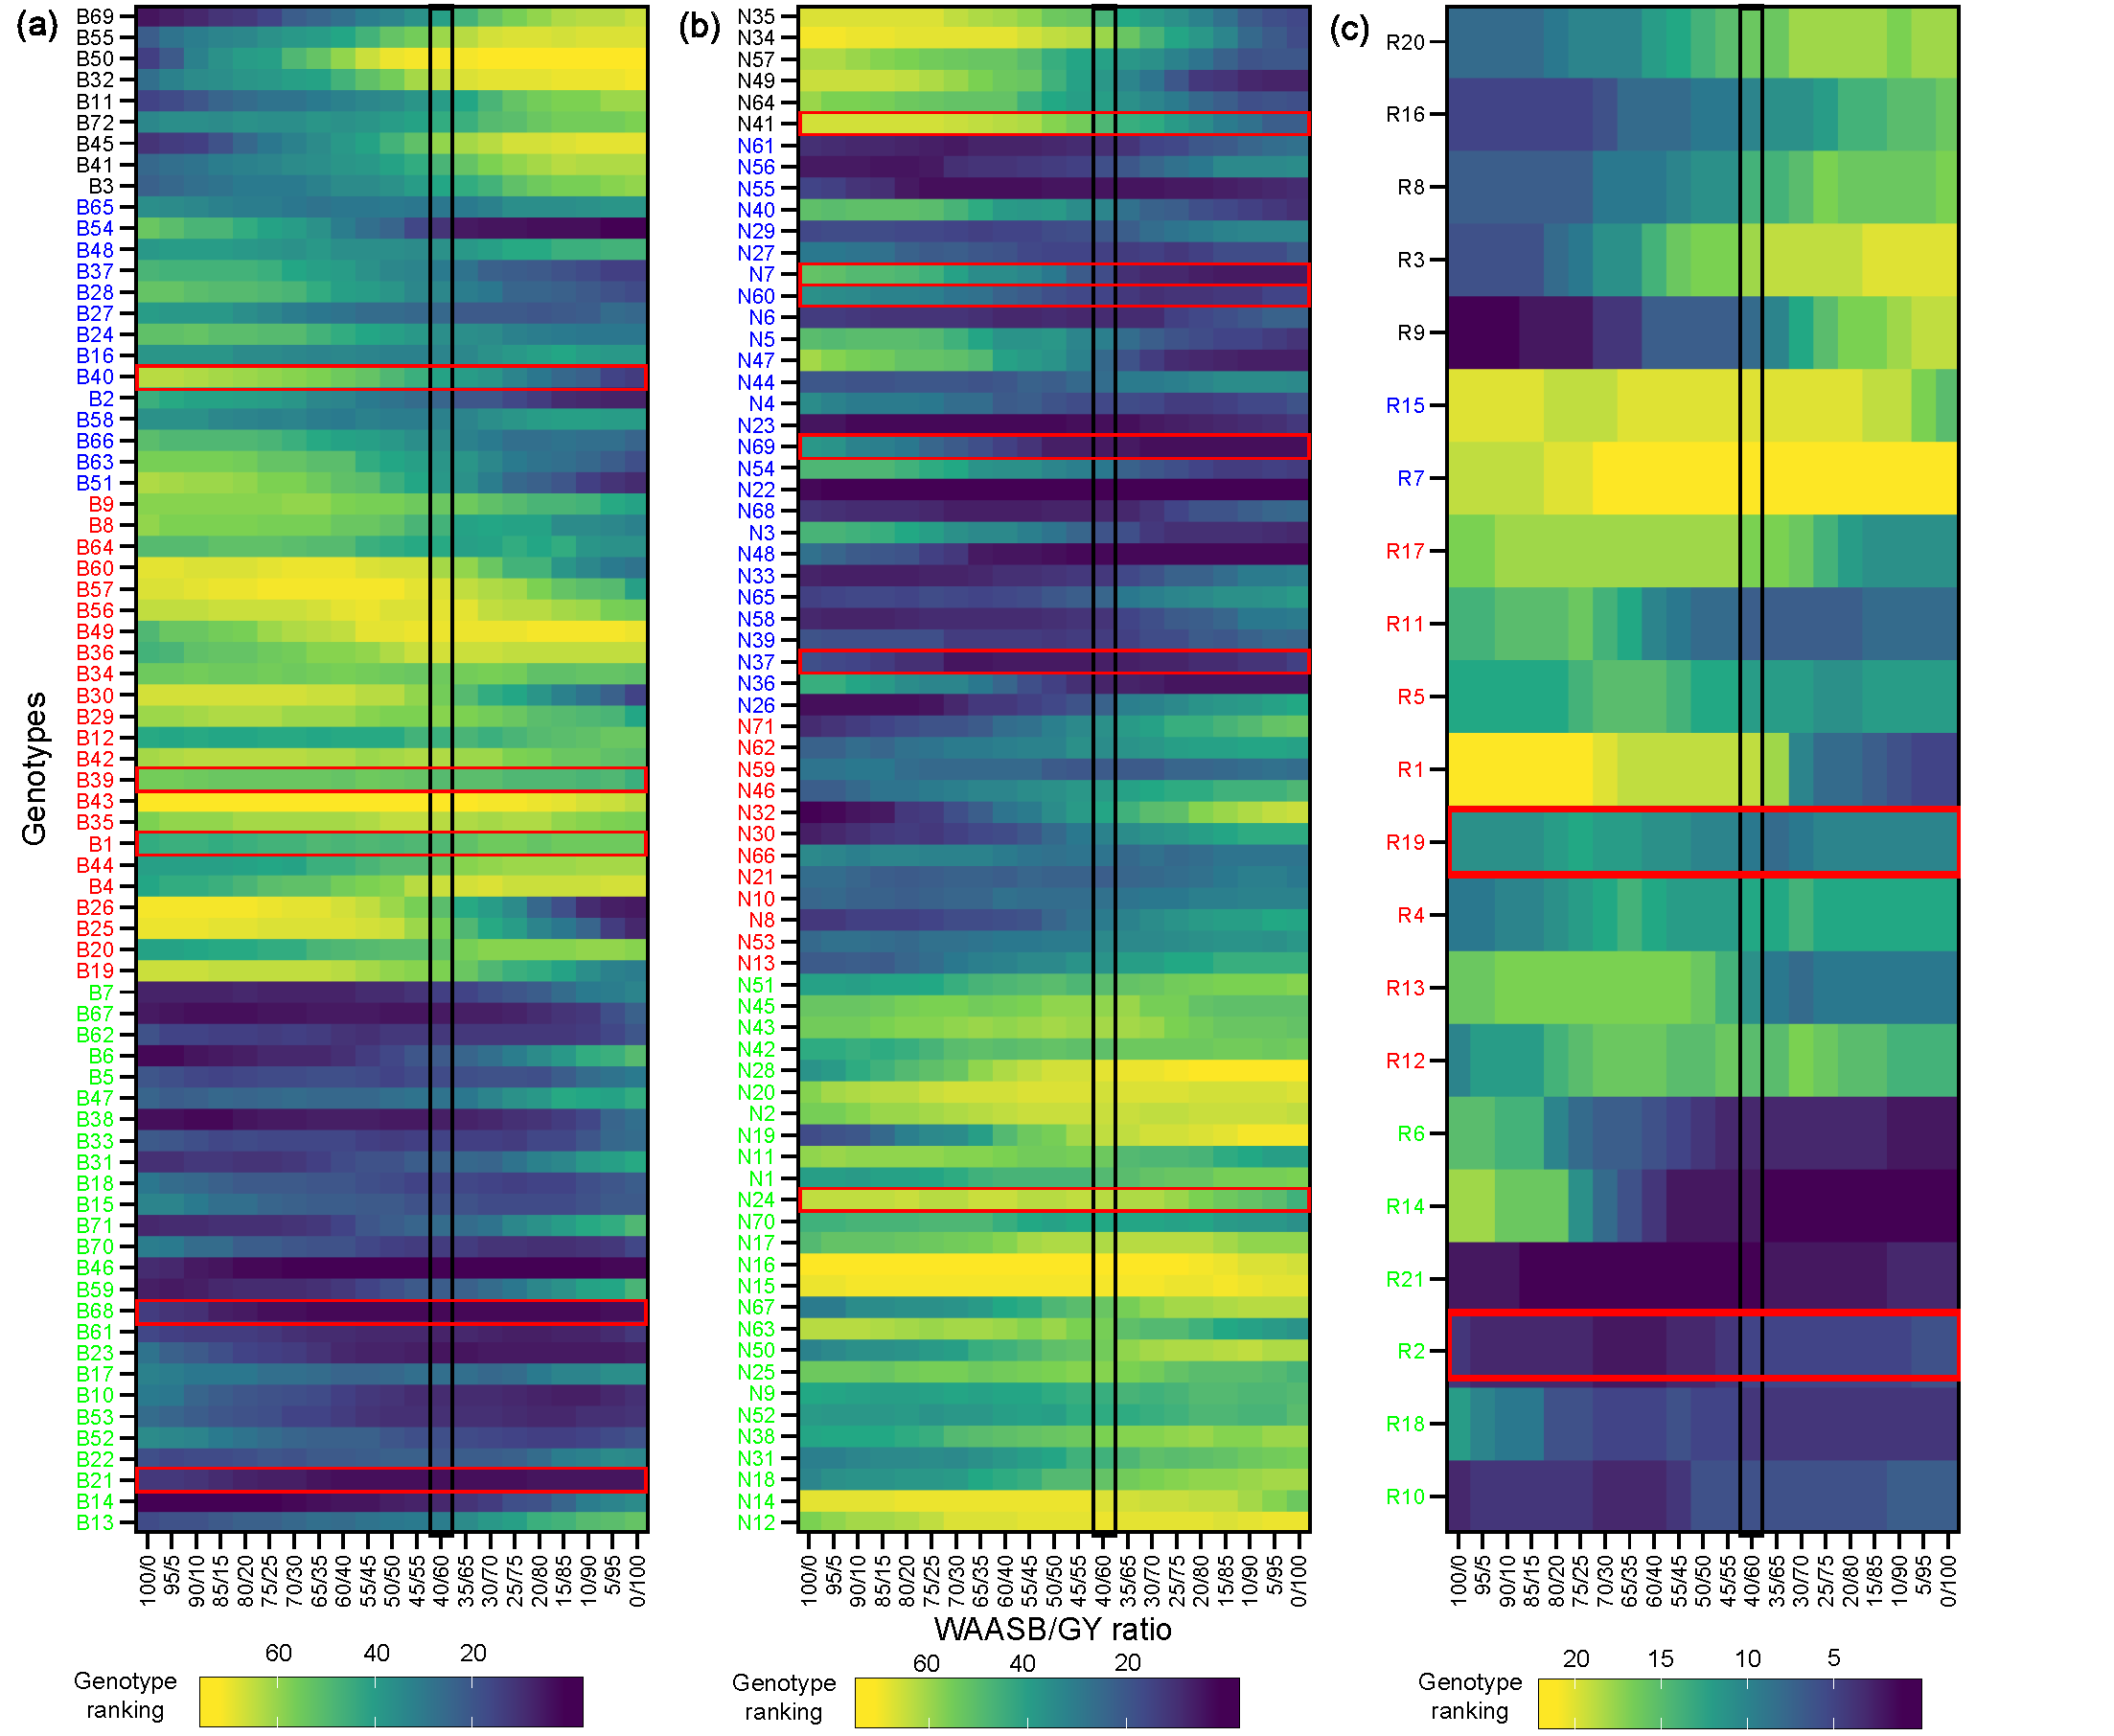
\includegraphics[width=1\linewidth]{main-figures/waasb_ratio_new} 

}

\caption{Supplemental Figure S12: Ranks of dry beans genotypes (a: 72 black, b:71 navys and c: 21 small red/pink) considering different weights for stability and yielding. The most-left ranks were obtained considering the stability only. The most right-ranks were obtained considering the grain yield only. Between the extremes, ranks were obtained different weights for stability and yielding. The four clusters represent four classes of genotypes: (1) Poorly productive and unstable genotypes; (2) productive but unstable genotypes; (3) stable but poorly productive genotypes; and (4), highly productive and stable genotypes. The ranks highlighted by a black rectangle are the same as those BLUPs predicted to WAASBY index and the red rectangle box are the selected genotypes by the Multi-Trait Stability Index (MTSI).}\label{fig:selected waasb}
\end{figure}

\pagebreak

\begin{figure}[H]

{\centering 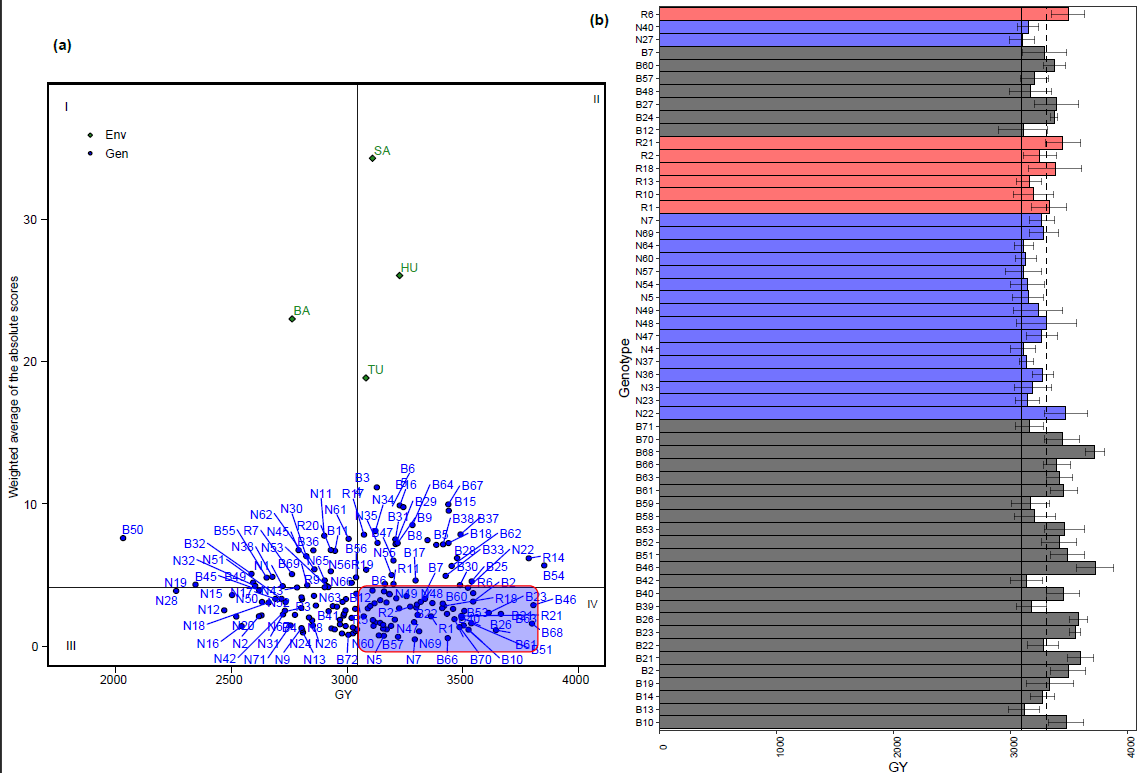
\includegraphics[width=1\linewidth]{main-figures/S13} 

}

\caption{Supplemental Figure S13: Joint interpretation for mean performance and stability for grain yield (GY) in Kg/ha (a) and mean performance (b) for grain yield (GY) analysis. The vertical dashed and solid lines show, respectively, the mean of the selected genotype and the overall mean for both mean performance and WAASB index. Black, Navy and Small Red beans are represented by bars colors black, blue and red. The x axis shows the arithmetic mean for each genotype × environment interaction and y axis the weighted average of absolute scores from the singular value decomposition of the matrix of best linear unbiased predictions for the genotype × environment interaction effects generated by a combined linear mixed-effect model (WAASB) of 72 Black, 71 Navy and 21 Small Red beans evaluated in 4 environments (BA: Bay, HU: Huron, SA: Sanilac, TU: Tuscola). The blue shaded squared in the quadrant IV are the potential selected genotypes considering combined analysis.}\label{fig:s13}
\end{figure}

\pagebreak

\begin{figure}[H]

{\centering 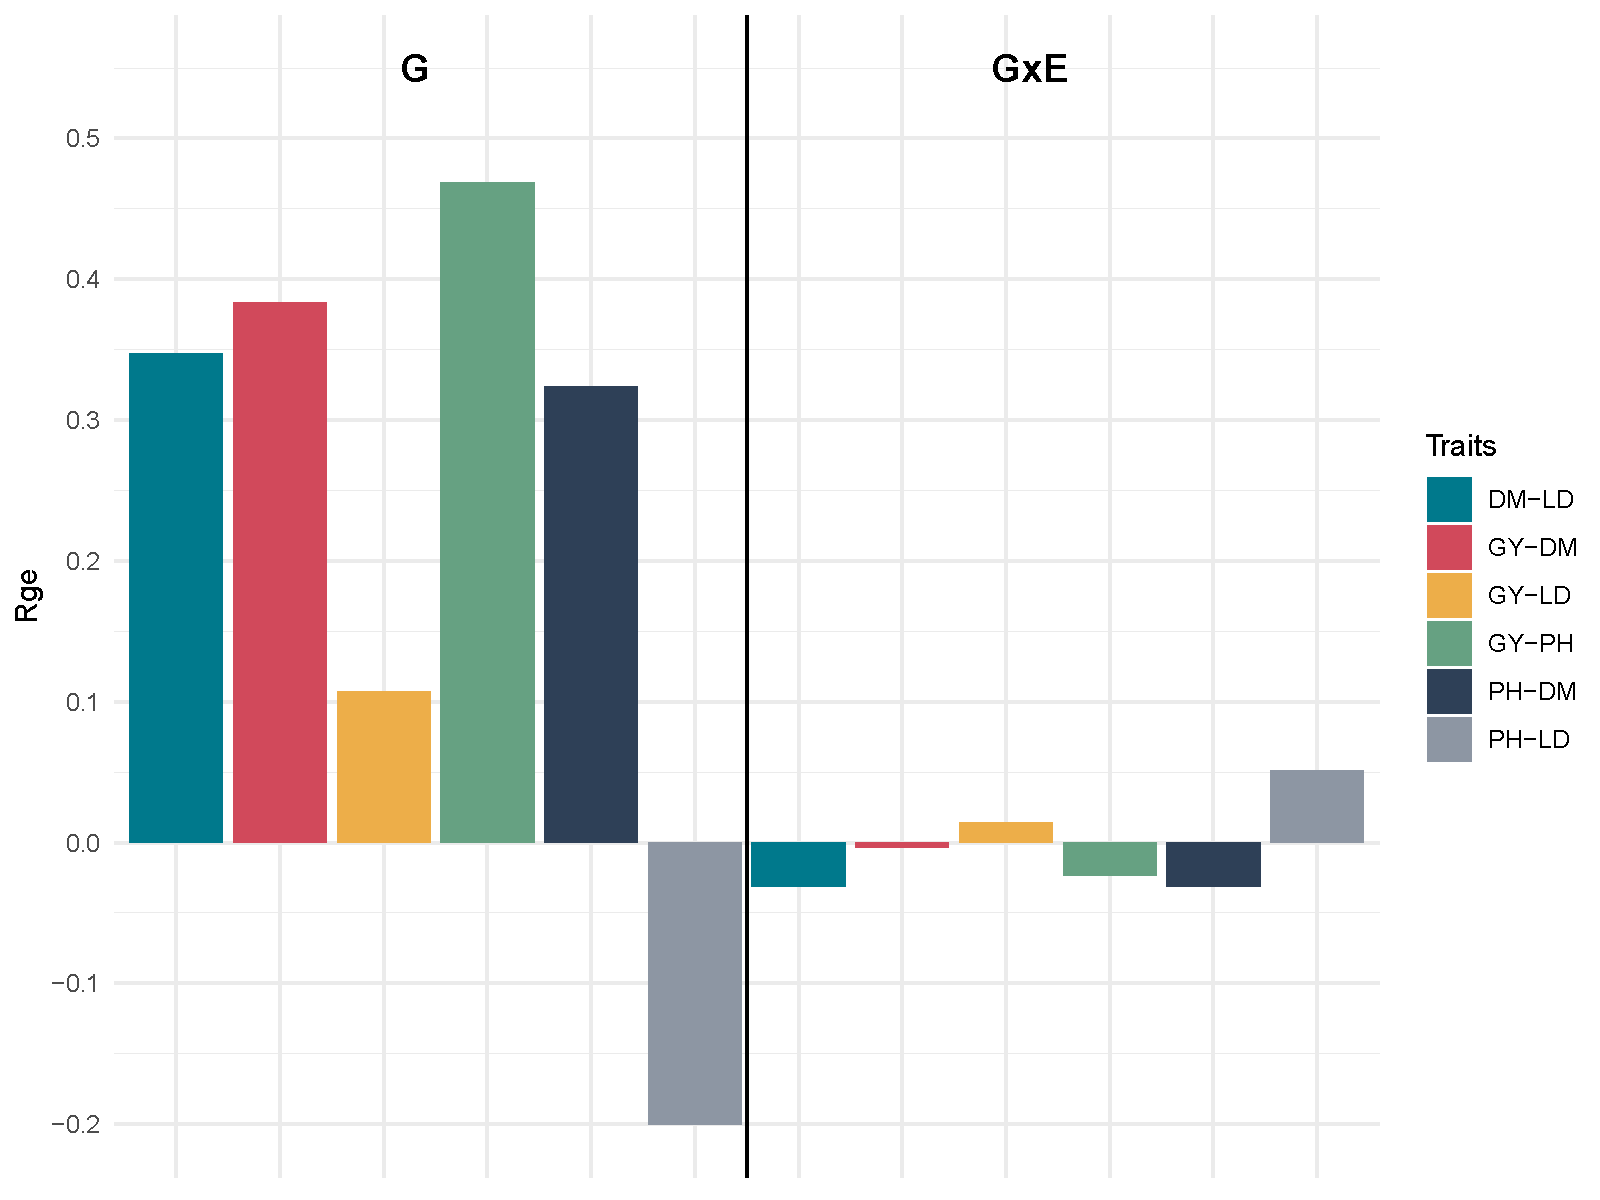
\includegraphics[width=1\linewidth]{main-figures/Rplot_MTME-allmkt} 

}

\caption{Supplemental Figure S14: MTME model: Genotypic correlation between GY, DPM, and PH across genotypes and locations for all market classes (BB, NB, and SR) combined analysis (CombMKT). The genotype (G) and genotype × environment interactions (GEI) correlation coefficients between the GY, DM, PH, and LD traits.}\label{fig:s14}
\end{figure}

\pagebreak

\pagebreak

\hypertarget{appendix-c---r-codes}{%
\section{Appendix C - R codes}\label{appendix-c---r-codes}}

\hypertarget{getting-started}{%
\section*{Getting started}\label{getting-started}}
\addcontentsline{toc}{section}{Getting started}

The present analysis aims to dissect the genotype by environment
interaction study (aka GEI) using a data set from the Dry Beans breeding
program at Michigan State University - MSU.

The trait in study is the grain yield (GY) per plot (lb/plot) adjusted
to the international measurements (Kg/ha). A previous data analysis (not
shown here) was done to perform the historical data mining and adjust of
raw data. Besides the GY, plant height (PH), date of maturity (DM) and
lodging (LD) were investigate using a subset from 2021, which contains
the all the data available.

The main focus of this manuscript, as describe in the
\href{link\%20here}{published paper}, is to investigate the varieties
performance of GY across four locations at different Michigan counties.
However, the MTME (three locations and 4 traits) also was studied in
this manuscript when available (only in 2021 in Bay, Tuscola and Sanilac
sites). Thus, different types of analysis will be performed in order to
study the GEI in the Multi-Environment-Trials (MET) data to provide
better varieties recommendations to the Dry Beans breeding program,
which:

\begin{itemize}
\tightlist
\item[$\boxtimes$]
  Multi-Environment Trials -- Genotype x Environment Interaction to
  grain yield (GY)
\item[$\boxtimes$]
  Mean performance and stability of multiple traits
\end{itemize}

\hypertarget{packages}{%
\subsection{Packages}\label{packages}}

R packages version from: 2024-01-03.

The analysis was done using the R Statistical language (v4.3.1; R Core
Team, 2023) on Windows 10 x64, using the packages rmarkdown (v2.25),
ggpmisc (v0.5.4.1), ggpp (v0.5.4), gridExtra (v2.3), magrittr (v2.0.3),
Matrix (v1.6.1.1), mapdata (v2.3.1), maps (v3.4.1), effectsize (v0.8.6),
spData (v2.3.0), asremlPlus (v4.4.15), tidyquant (v1.0.7), usmap
(v0.6.4), data.table (v1.14.8), ggspatial (v1.1.9), ggpattern (v1.0.1),
viridisLite (v0.4.2), viridis (v0.6.4), flextable (v0.9.3), lubridate
(v1.9.3), raster (v3.6.26), ggcorrplot (v0.1.4.1), ggdist (v3.3.1),
parameters (v0.21.2), performance (v0.10.5), easystats (v0.6.0), see
(v0.8.0), insight (v0.19.6), bayestestR (v0.13.1), modelbased (v0.8.6),
report (v0.5.7), correlation (v0.8.4), tibble (v3.2.1), RColorBrewer
(v1.1.3), rcartocolor (v2.1.1), metan (v1.18.0), ggstatsplot (v0.12.1),
datawizard (v0.9.0), sp (v2.1.1), sf (v1.0.14), ggforce (v0.4.1),
patchwork (v1.1.3), PerformanceAnalytics (v2.0.4), broom (v1.0.5),
quantmod (v0.4.25), xts (v0.13.1), openxlsx (v4.2.5.2), asreml
(v4.2.0.267), naniar (v1.0.0), TTR (v0.24.4), statgenGxE (v1.0.5),
tigris (v2.0.4), plyr (v1.8.9), ggplot2 (v3.4.4), stringr (v1.5.0),
forcats (v1.0.0), tidyverse (v2.0.0), dplyr (v1.1.4), purrr (v1.0.2),
readr (v2.1.4), tidyr (v1.3.0), cowplot (v1.1.1), nadiv (v2.17.2), DT
(v0.30), zoo (v1.8.12) and kableExtra (v1.3.4).

\hypertarget{data-preparation}{%
\subsection{Data preparation}\label{data-preparation}}

\begin{Shaded}
\begin{Highlighting}[]
\NormalTok{data\_beans }\OtherTok{=} \FunctionTok{read.csv}\NormalTok{(}\StringTok{"data/DataBean\_MET\_GYv2.csv"}\NormalTok{,}\AttributeTok{h=}\NormalTok{T, }\AttributeTok{stringsAsFactors =}\NormalTok{ T)}

\ControlFlowTok{if}\NormalTok{ (knitr}\SpecialCharTok{::}\FunctionTok{is\_html\_output}\NormalTok{()) \{}

  \FunctionTok{print\_table}\NormalTok{(data\_beans)}
  
\NormalTok{\}}\ControlFlowTok{else}\NormalTok{\{}
  
  \FunctionTok{flextable}\NormalTok{(}\FunctionTok{head}\NormalTok{(data\_beans)) }\SpecialCharTok{\%\textgreater{}\%}
   \FunctionTok{add\_footer\_lines}\NormalTok{(}
     \FunctionTok{c}\NormalTok{(}\StringTok{"Varieties Dry Beans data set from 2017 to 2022"}\NormalTok{,}
       \StringTok{"Header data set showing the 6 first entry"}\NormalTok{)) }\SpecialCharTok{\%\textgreater{}\%}
   \FunctionTok{autofit}\NormalTok{() }\SpecialCharTok{\%\textgreater{}\%}
   \FunctionTok{add\_header\_lines}\NormalTok{(}\StringTok{"Dry Beans varieties trial"}\NormalTok{) }\SpecialCharTok{\%\textgreater{}\%}
  \FunctionTok{theme\_design2}\NormalTok{()}
\NormalTok{\}}
\end{Highlighting}
\end{Shaded}

\global\setlength{\Oldarrayrulewidth}{\arrayrulewidth}

\global\setlength{\Oldtabcolsep}{\tabcolsep}

\setlength{\tabcolsep}{0pt}

\renewcommand*{\arraystretch}{1.5}



\providecommand{\ascline}[3]{\noalign{\global\arrayrulewidth #1}\arrayrulecolor[HTML]{#2}\cline{#3}}

\begin{longtable}[c]{|p{0.90in}|p{0.75in}|p{0.75in}|p{0.75in}|p{0.77in}|p{0.75in}|p{0.75in}|p{0.85in}}



\ascline{1.5pt}{666666}{1-8}

\multicolumn{8}{>{\raggedright}m{\dimexpr 6.27in+14\tabcolsep}}{\textcolor[HTML]{000000}{\fontsize{10}{10}\selectfont{\global\setmainfont{Arial}{\textbf{Dry\ Beans\ varieties\ trial}}}}} \\

\ascline{0.75pt}{666666}{1-8}



\multicolumn{1}{>{\raggedright}m{\dimexpr 0.9in+0\tabcolsep}}{\textcolor[HTML]{000000}{\fontsize{10}{10}\selectfont{\global\setmainfont{Arial}{\textbf{codename}}}}} & \multicolumn{1}{>{\raggedright}m{\dimexpr 0.75in+0\tabcolsep}}{\textcolor[HTML]{000000}{\fontsize{10}{10}\selectfont{\global\setmainfont{Arial}{\textbf{name}}}}} & \multicolumn{1}{>{\raggedleft}m{\dimexpr 0.75in+0\tabcolsep}}{\textcolor[HTML]{000000}{\fontsize{10}{10}\selectfont{\global\setmainfont{Arial}{\textbf{rep}}}}} & \multicolumn{1}{>{\raggedright}m{\dimexpr 0.75in+0\tabcolsep}}{\textcolor[HTML]{000000}{\fontsize{10}{10}\selectfont{\global\setmainfont{Arial}{\textbf{mkt}}}}} & \multicolumn{1}{>{\raggedright}m{\dimexpr 0.77in+0\tabcolsep}}{\textcolor[HTML]{000000}{\fontsize{10}{10}\selectfont{\global\setmainfont{Arial}{\textbf{year\_loc}}}}} & \multicolumn{1}{>{\raggedright}m{\dimexpr 0.75in+0\tabcolsep}}{\textcolor[HTML]{000000}{\fontsize{10}{10}\selectfont{\global\setmainfont{Arial}{\textbf{loc}}}}} & \multicolumn{1}{>{\raggedleft}m{\dimexpr 0.75in+0\tabcolsep}}{\textcolor[HTML]{000000}{\fontsize{10}{10}\selectfont{\global\setmainfont{Arial}{\textbf{year}}}}} & \multicolumn{1}{>{\raggedleft}m{\dimexpr 0.85in+0\tabcolsep}}{\textcolor[HTML]{000000}{\fontsize{10}{10}\selectfont{\global\setmainfont{Arial}{\textbf{gy\_kg\_ha}}}}} \\

\ascline{1.5pt}{666666}{1-8}\endfirsthead

\ascline{1.5pt}{666666}{1-8}

\multicolumn{8}{>{\raggedright}m{\dimexpr 6.27in+14\tabcolsep}}{\textcolor[HTML]{000000}{\fontsize{10}{10}\selectfont{\global\setmainfont{Arial}{\textbf{Dry\ Beans\ varieties\ trial}}}}} \\

\ascline{0.75pt}{666666}{1-8}



\multicolumn{1}{>{\raggedright}m{\dimexpr 0.9in+0\tabcolsep}}{\textcolor[HTML]{000000}{\fontsize{10}{10}\selectfont{\global\setmainfont{Arial}{\textbf{codename}}}}} & \multicolumn{1}{>{\raggedright}m{\dimexpr 0.75in+0\tabcolsep}}{\textcolor[HTML]{000000}{\fontsize{10}{10}\selectfont{\global\setmainfont{Arial}{\textbf{name}}}}} & \multicolumn{1}{>{\raggedleft}m{\dimexpr 0.75in+0\tabcolsep}}{\textcolor[HTML]{000000}{\fontsize{10}{10}\selectfont{\global\setmainfont{Arial}{\textbf{rep}}}}} & \multicolumn{1}{>{\raggedright}m{\dimexpr 0.75in+0\tabcolsep}}{\textcolor[HTML]{000000}{\fontsize{10}{10}\selectfont{\global\setmainfont{Arial}{\textbf{mkt}}}}} & \multicolumn{1}{>{\raggedright}m{\dimexpr 0.77in+0\tabcolsep}}{\textcolor[HTML]{000000}{\fontsize{10}{10}\selectfont{\global\setmainfont{Arial}{\textbf{year\_loc}}}}} & \multicolumn{1}{>{\raggedright}m{\dimexpr 0.75in+0\tabcolsep}}{\textcolor[HTML]{000000}{\fontsize{10}{10}\selectfont{\global\setmainfont{Arial}{\textbf{loc}}}}} & \multicolumn{1}{>{\raggedleft}m{\dimexpr 0.75in+0\tabcolsep}}{\textcolor[HTML]{000000}{\fontsize{10}{10}\selectfont{\global\setmainfont{Arial}{\textbf{year}}}}} & \multicolumn{1}{>{\raggedleft}m{\dimexpr 0.85in+0\tabcolsep}}{\textcolor[HTML]{000000}{\fontsize{10}{10}\selectfont{\global\setmainfont{Arial}{\textbf{gy\_kg\_ha}}}}} \\

\ascline{1.5pt}{666666}{1-8}\endhead



\multicolumn{8}{>{\raggedright}m{\dimexpr 6.27in+14\tabcolsep}}{\textcolor[HTML]{000000}{\fontsize{8}{8}\selectfont{\global\setmainfont{Arial}{Varieties\ Dry\ Beans\ data\ set\ from\ 2017\ to\ 2022}}}} \\

\ascline{0.75pt}{666666}{1-8}



\multicolumn{8}{>{\raggedright}m{\dimexpr 6.27in+14\tabcolsep}}{\textcolor[HTML]{000000}{\fontsize{8}{8}\selectfont{\global\setmainfont{Arial}{Header\ data\ set\ showing\ the\ 6\ first\ entry}}}} \\

\ascline{0.75pt}{666666}{1-8}\endfoot



\multicolumn{1}{>{\raggedright}m{\dimexpr 0.9in+0\tabcolsep}}{\textcolor[HTML]{000000}{\fontsize{9}{9}\selectfont{\global\setmainfont{Arial}{213SP}}}} & \multicolumn{1}{>{\raggedright}m{\dimexpr 0.75in+0\tabcolsep}}{\textcolor[HTML]{000000}{\fontsize{9}{9}\selectfont{\global\setmainfont{Arial}{N1}}}} & \multicolumn{1}{>{\raggedleft}m{\dimexpr 0.75in+0\tabcolsep}}{\textcolor[HTML]{000000}{\fontsize{9}{9}\selectfont{\global\setmainfont{Arial}{1}}}} & \multicolumn{1}{>{\raggedright}m{\dimexpr 0.75in+0\tabcolsep}}{\textcolor[HTML]{000000}{\fontsize{9}{9}\selectfont{\global\setmainfont{Arial}{NB}}}} & \multicolumn{1}{>{\raggedright}m{\dimexpr 0.77in+0\tabcolsep}}{\textcolor[HTML]{000000}{\fontsize{9}{9}\selectfont{\global\setmainfont{Arial}{17\_BA}}}} & \multicolumn{1}{>{\raggedright}m{\dimexpr 0.75in+0\tabcolsep}}{\textcolor[HTML]{000000}{\fontsize{9}{9}\selectfont{\global\setmainfont{Arial}{BA}}}} & \multicolumn{1}{>{\raggedleft}m{\dimexpr 0.75in+0\tabcolsep}}{\textcolor[HTML]{000000}{\fontsize{9}{9}\selectfont{\global\setmainfont{Arial}{17}}}} & \multicolumn{1}{>{\raggedleft}m{\dimexpr 0.85in+0\tabcolsep}}{\textcolor[HTML]{000000}{\fontsize{9}{9}\selectfont{\global\setmainfont{Arial}{}}}} \\

\ascline{0.75pt}{666666}{1-8}



\multicolumn{1}{>{\raggedright}m{\dimexpr 0.9in+0\tabcolsep}}{\textcolor[HTML]{000000}{\fontsize{9}{9}\selectfont{\global\setmainfont{Arial}{213SP}}}} & \multicolumn{1}{>{\raggedright}m{\dimexpr 0.75in+0\tabcolsep}}{\textcolor[HTML]{000000}{\fontsize{9}{9}\selectfont{\global\setmainfont{Arial}{N1}}}} & \multicolumn{1}{>{\raggedleft}m{\dimexpr 0.75in+0\tabcolsep}}{\textcolor[HTML]{000000}{\fontsize{9}{9}\selectfont{\global\setmainfont{Arial}{1}}}} & \multicolumn{1}{>{\raggedright}m{\dimexpr 0.75in+0\tabcolsep}}{\textcolor[HTML]{000000}{\fontsize{9}{9}\selectfont{\global\setmainfont{Arial}{NB}}}} & \multicolumn{1}{>{\raggedright}m{\dimexpr 0.77in+0\tabcolsep}}{\textcolor[HTML]{000000}{\fontsize{9}{9}\selectfont{\global\setmainfont{Arial}{17\_HU}}}} & \multicolumn{1}{>{\raggedright}m{\dimexpr 0.75in+0\tabcolsep}}{\textcolor[HTML]{000000}{\fontsize{9}{9}\selectfont{\global\setmainfont{Arial}{HU}}}} & \multicolumn{1}{>{\raggedleft}m{\dimexpr 0.75in+0\tabcolsep}}{\textcolor[HTML]{000000}{\fontsize{9}{9}\selectfont{\global\setmainfont{Arial}{17}}}} & \multicolumn{1}{>{\raggedleft}m{\dimexpr 0.85in+0\tabcolsep}}{\textcolor[HTML]{000000}{\fontsize{9}{9}\selectfont{\global\setmainfont{Arial}{}}}} \\

\ascline{0.75pt}{666666}{1-8}



\multicolumn{1}{>{\raggedright}m{\dimexpr 0.9in+0\tabcolsep}}{\textcolor[HTML]{000000}{\fontsize{9}{9}\selectfont{\global\setmainfont{Arial}{213SP}}}} & \multicolumn{1}{>{\raggedright}m{\dimexpr 0.75in+0\tabcolsep}}{\textcolor[HTML]{000000}{\fontsize{9}{9}\selectfont{\global\setmainfont{Arial}{N1}}}} & \multicolumn{1}{>{\raggedleft}m{\dimexpr 0.75in+0\tabcolsep}}{\textcolor[HTML]{000000}{\fontsize{9}{9}\selectfont{\global\setmainfont{Arial}{1}}}} & \multicolumn{1}{>{\raggedright}m{\dimexpr 0.75in+0\tabcolsep}}{\textcolor[HTML]{000000}{\fontsize{9}{9}\selectfont{\global\setmainfont{Arial}{NB}}}} & \multicolumn{1}{>{\raggedright}m{\dimexpr 0.77in+0\tabcolsep}}{\textcolor[HTML]{000000}{\fontsize{9}{9}\selectfont{\global\setmainfont{Arial}{17\_SA}}}} & \multicolumn{1}{>{\raggedright}m{\dimexpr 0.75in+0\tabcolsep}}{\textcolor[HTML]{000000}{\fontsize{9}{9}\selectfont{\global\setmainfont{Arial}{SA}}}} & \multicolumn{1}{>{\raggedleft}m{\dimexpr 0.75in+0\tabcolsep}}{\textcolor[HTML]{000000}{\fontsize{9}{9}\selectfont{\global\setmainfont{Arial}{17}}}} & \multicolumn{1}{>{\raggedleft}m{\dimexpr 0.85in+0\tabcolsep}}{\textcolor[HTML]{000000}{\fontsize{9}{9}\selectfont{\global\setmainfont{Arial}{}}}} \\

\ascline{0.75pt}{666666}{1-8}



\multicolumn{1}{>{\raggedright}m{\dimexpr 0.9in+0\tabcolsep}}{\textcolor[HTML]{000000}{\fontsize{9}{9}\selectfont{\global\setmainfont{Arial}{213SP}}}} & \multicolumn{1}{>{\raggedright}m{\dimexpr 0.75in+0\tabcolsep}}{\textcolor[HTML]{000000}{\fontsize{9}{9}\selectfont{\global\setmainfont{Arial}{N1}}}} & \multicolumn{1}{>{\raggedleft}m{\dimexpr 0.75in+0\tabcolsep}}{\textcolor[HTML]{000000}{\fontsize{9}{9}\selectfont{\global\setmainfont{Arial}{1}}}} & \multicolumn{1}{>{\raggedright}m{\dimexpr 0.75in+0\tabcolsep}}{\textcolor[HTML]{000000}{\fontsize{9}{9}\selectfont{\global\setmainfont{Arial}{NB}}}} & \multicolumn{1}{>{\raggedright}m{\dimexpr 0.77in+0\tabcolsep}}{\textcolor[HTML]{000000}{\fontsize{9}{9}\selectfont{\global\setmainfont{Arial}{17\_TU}}}} & \multicolumn{1}{>{\raggedright}m{\dimexpr 0.75in+0\tabcolsep}}{\textcolor[HTML]{000000}{\fontsize{9}{9}\selectfont{\global\setmainfont{Arial}{TU}}}} & \multicolumn{1}{>{\raggedleft}m{\dimexpr 0.75in+0\tabcolsep}}{\textcolor[HTML]{000000}{\fontsize{9}{9}\selectfont{\global\setmainfont{Arial}{17}}}} & \multicolumn{1}{>{\raggedleft}m{\dimexpr 0.85in+0\tabcolsep}}{\textcolor[HTML]{000000}{\fontsize{9}{9}\selectfont{\global\setmainfont{Arial}{}}}} \\

\ascline{0.75pt}{666666}{1-8}



\multicolumn{1}{>{\raggedright}m{\dimexpr 0.9in+0\tabcolsep}}{\textcolor[HTML]{000000}{\fontsize{9}{9}\selectfont{\global\setmainfont{Arial}{213SP}}}} & \multicolumn{1}{>{\raggedright}m{\dimexpr 0.75in+0\tabcolsep}}{\textcolor[HTML]{000000}{\fontsize{9}{9}\selectfont{\global\setmainfont{Arial}{N1}}}} & \multicolumn{1}{>{\raggedleft}m{\dimexpr 0.75in+0\tabcolsep}}{\textcolor[HTML]{000000}{\fontsize{9}{9}\selectfont{\global\setmainfont{Arial}{1}}}} & \multicolumn{1}{>{\raggedright}m{\dimexpr 0.75in+0\tabcolsep}}{\textcolor[HTML]{000000}{\fontsize{9}{9}\selectfont{\global\setmainfont{Arial}{NB}}}} & \multicolumn{1}{>{\raggedright}m{\dimexpr 0.77in+0\tabcolsep}}{\textcolor[HTML]{000000}{\fontsize{9}{9}\selectfont{\global\setmainfont{Arial}{18\_BA}}}} & \multicolumn{1}{>{\raggedright}m{\dimexpr 0.75in+0\tabcolsep}}{\textcolor[HTML]{000000}{\fontsize{9}{9}\selectfont{\global\setmainfont{Arial}{BA}}}} & \multicolumn{1}{>{\raggedleft}m{\dimexpr 0.75in+0\tabcolsep}}{\textcolor[HTML]{000000}{\fontsize{9}{9}\selectfont{\global\setmainfont{Arial}{18}}}} & \multicolumn{1}{>{\raggedleft}m{\dimexpr 0.85in+0\tabcolsep}}{\textcolor[HTML]{000000}{\fontsize{9}{9}\selectfont{\global\setmainfont{Arial}{}}}} \\

\ascline{0.75pt}{666666}{1-8}



\multicolumn{1}{>{\raggedright}m{\dimexpr 0.9in+0\tabcolsep}}{\textcolor[HTML]{000000}{\fontsize{9}{9}\selectfont{\global\setmainfont{Arial}{213SP}}}} & \multicolumn{1}{>{\raggedright}m{\dimexpr 0.75in+0\tabcolsep}}{\textcolor[HTML]{000000}{\fontsize{9}{9}\selectfont{\global\setmainfont{Arial}{N1}}}} & \multicolumn{1}{>{\raggedleft}m{\dimexpr 0.75in+0\tabcolsep}}{\textcolor[HTML]{000000}{\fontsize{9}{9}\selectfont{\global\setmainfont{Arial}{1}}}} & \multicolumn{1}{>{\raggedright}m{\dimexpr 0.75in+0\tabcolsep}}{\textcolor[HTML]{000000}{\fontsize{9}{9}\selectfont{\global\setmainfont{Arial}{NB}}}} & \multicolumn{1}{>{\raggedright}m{\dimexpr 0.77in+0\tabcolsep}}{\textcolor[HTML]{000000}{\fontsize{9}{9}\selectfont{\global\setmainfont{Arial}{18\_HU}}}} & \multicolumn{1}{>{\raggedright}m{\dimexpr 0.75in+0\tabcolsep}}{\textcolor[HTML]{000000}{\fontsize{9}{9}\selectfont{\global\setmainfont{Arial}{HU}}}} & \multicolumn{1}{>{\raggedleft}m{\dimexpr 0.75in+0\tabcolsep}}{\textcolor[HTML]{000000}{\fontsize{9}{9}\selectfont{\global\setmainfont{Arial}{18}}}} & \multicolumn{1}{>{\raggedleft}m{\dimexpr 0.85in+0\tabcolsep}}{\textcolor[HTML]{000000}{\fontsize{9}{9}\selectfont{\global\setmainfont{Arial}{}}}} \\

\ascline{1.5pt}{666666}{1-8}



\end{longtable}



\arrayrulecolor[HTML]{000000}

\global\setlength{\arrayrulewidth}{\Oldarrayrulewidth}

\global\setlength{\tabcolsep}{\Oldtabcolsep}

\renewcommand*{\arraystretch}{1}

\begin{Shaded}
\begin{Highlighting}[]
\CommentTok{\# Data adjustment}
\CommentTok{\# All the effect columns must be as a factor to run in ASReml{-}r.}
\NormalTok{cols }\OtherTok{\textless{}{-}} \FunctionTok{c}\NormalTok{(}\StringTok{"rep"}\NormalTok{, }\StringTok{"name"}\NormalTok{, }\StringTok{"loc"}\NormalTok{,}\StringTok{"year"}\NormalTok{, }\StringTok{"mkt"}\NormalTok{, }\StringTok{"year\_loc"}\NormalTok{)}
\NormalTok{data\_beans[cols] }\OtherTok{\textless{}{-}} \FunctionTok{lapply}\NormalTok{(data\_beans[cols], factor)}
\NormalTok{data\_beans }\OtherTok{\textless{}{-}} \FunctionTok{data.table}\NormalTok{(data\_beans)}
\end{Highlighting}
\end{Shaded}

\hypertarget{descriptive-stats---raw-data}{%
\subsection{Descriptive Stats - Raw
data}\label{descriptive-stats---raw-data}}

Data set distribution, checking data and locations of study.

\begin{Shaded}
\begin{Highlighting}[]
\NormalTok{data\_beans }\OtherTok{=} \FunctionTok{read.csv}\NormalTok{(}\StringTok{"data/DataBean\_MET\_GYv2.csv"}\NormalTok{,}\AttributeTok{h=}\NormalTok{T, }\AttributeTok{stringsAsFactors =}\NormalTok{ T)}

\CommentTok{\# Data adjustment}
\CommentTok{\# All the effect columns must be as a factor to run in ASReml{-}r.}
\NormalTok{cols }\OtherTok{\textless{}{-}} \FunctionTok{c}\NormalTok{(}\StringTok{"rep"}\NormalTok{, }\StringTok{"name"}\NormalTok{, }\StringTok{"loc"}\NormalTok{,}\StringTok{"year"}\NormalTok{, }\StringTok{"mkt"}\NormalTok{, }\StringTok{"year\_loc"}\NormalTok{)}
\NormalTok{data\_beans[cols] }\OtherTok{\textless{}{-}} \FunctionTok{lapply}\NormalTok{(data\_beans[cols], factor)}
\NormalTok{data\_beans }\OtherTok{\textless{}{-}} \FunctionTok{data.table}\NormalTok{(data\_beans)}
\end{Highlighting}
\end{Shaded}

\hypertarget{box-plot-dist.}{%
\subsubsection{Box plot dist.}\label{box-plot-dist.}}

\begin{Shaded}
\begin{Highlighting}[]
\NormalTok{plotDM\_stats\_mkt\_loc}\OtherTok{\textless{}{-}} \FunctionTok{grouped\_ggbetweenstats}\NormalTok{(}\AttributeTok{data=}\NormalTok{data\_beans, }\AttributeTok{x=}\NormalTok{ loc, }\AttributeTok{y=}\NormalTok{gy\_kg\_ha, }\AttributeTok{type =} \StringTok{"parametric"}\NormalTok{,  }\AttributeTok{bf.message =}\NormalTok{ F, }\AttributeTok{results.subtitle =}\NormalTok{ F, }
                              \AttributeTok{ylab=} \StringTok{"GY"}\NormalTok{, }\AttributeTok{xlab =} \StringTok{"Locations"}\NormalTok{,}
                              \AttributeTok{plot.type =} \StringTok{"boxviolin"}\NormalTok{, }\AttributeTok{grouping.var =}\NormalTok{ mkt ) }
\CommentTok{\#print(plotDM\_stats\_mkt\_loc)}

\NormalTok{plotDM\_stats\_mkt\_year}\OtherTok{\textless{}{-}} \FunctionTok{grouped\_ggbetweenstats}\NormalTok{(}\AttributeTok{data=}\NormalTok{data\_beans, }\AttributeTok{x=}\NormalTok{ year, }\AttributeTok{y=}\NormalTok{gy\_kg\_ha, }\AttributeTok{type =} \StringTok{"parametric"}\NormalTok{,  }\AttributeTok{bf.message =}\NormalTok{ F, }\AttributeTok{results.subtitle =}\NormalTok{ F, }
                              \AttributeTok{ylab=} \StringTok{"GY"}\NormalTok{, }\AttributeTok{xlab =} \StringTok{"Years"}\NormalTok{,}
                              \AttributeTok{plot.type =} \StringTok{"boxviolin"}\NormalTok{, }\AttributeTok{grouping.var =}\NormalTok{ mkt ) }
\CommentTok{\#print(plotDM\_stats\_mkt\_year)}

\FunctionTok{print}\NormalTok{(}\FunctionTok{arrange\_ggplot}\NormalTok{(plotDM\_stats\_mkt\_loc,plotDM\_stats\_mkt\_year))}
\end{Highlighting}
\end{Shaded}

\begin{Shaded}
\begin{Highlighting}[]
\NormalTok{a}\OtherTok{\textless{}{-}} \FunctionTok{ggplot}\NormalTok{(}\AttributeTok{data=}\NormalTok{data\_beans, }\FunctionTok{aes}\NormalTok{(}\AttributeTok{x=}\FunctionTok{reorder}\NormalTok{(loc, }\SpecialCharTok{{-}}\NormalTok{gy\_kg\_ha), }\AttributeTok{y=}\NormalTok{gy\_kg\_ha, }\AttributeTok{fill=}\NormalTok{loc)) }\SpecialCharTok{+}
\NormalTok{  ggdist}\SpecialCharTok{::}\FunctionTok{stat\_halfeye}\NormalTok{(}
    \AttributeTok{adjust =} \FloatTok{0.5}\NormalTok{,}
    \AttributeTok{justification =} \SpecialCharTok{{-}}\FloatTok{0.1}\NormalTok{,}
    \AttributeTok{.width =} \DecValTok{0}\NormalTok{,}
    \AttributeTok{point\_colour =} \ConstantTok{NA}
\NormalTok{  ) }\SpecialCharTok{+}
  
  \FunctionTok{geom\_boxplot}\NormalTok{( }
    \AttributeTok{width =}\NormalTok{ .}\DecValTok{12}\NormalTok{,}
   \CommentTok{\# outlier.color = NA,}
    \AttributeTok{alpha =} \FloatTok{0.5}\NormalTok{)}\SpecialCharTok{+}
\NormalTok{  tidyquant}\SpecialCharTok{::}\FunctionTok{theme\_tq}\NormalTok{()}\SpecialCharTok{+}
  \FunctionTok{facet\_wrap}\NormalTok{(}\StringTok{"year"}\NormalTok{)}\SpecialCharTok{+}
  \FunctionTok{facet\_grid}\NormalTok{(}\StringTok{"mkt"}\NormalTok{) }\SpecialCharTok{+}
\NormalTok{  tidyquant}\SpecialCharTok{::}\FunctionTok{scale\_fill\_tq}\NormalTok{() }\SpecialCharTok{+}
  \FunctionTok{scale\_x\_discrete}\NormalTok{(}\AttributeTok{expand =} \FunctionTok{c}\NormalTok{(}\FloatTok{0.03}\NormalTok{,}\DecValTok{0}\NormalTok{)) }\SpecialCharTok{+}
  \FunctionTok{scale\_y\_continuous}\NormalTok{(}\AttributeTok{limits =} \FunctionTok{c}\NormalTok{(}\DecValTok{1000}\NormalTok{,}\DecValTok{6000}\NormalTok{), }\AttributeTok{breaks =} \FunctionTok{seq}\NormalTok{(}\DecValTok{1000}\NormalTok{, }\DecValTok{6000}\NormalTok{, }\AttributeTok{by =} \DecValTok{1000}\NormalTok{)) }\SpecialCharTok{+}
  \FunctionTok{theme}\NormalTok{(}\AttributeTok{axis.text.x=}\FunctionTok{element\_text}\NormalTok{(}\AttributeTok{angle =} \DecValTok{90}\NormalTok{),}
        \AttributeTok{strip.text=}\FunctionTok{element\_blank}\NormalTok{(),}
        \AttributeTok{legend.position =} \StringTok{"none"}\NormalTok{,}
        \AttributeTok{panel.grid =} \FunctionTok{element\_blank}\NormalTok{())}\SpecialCharTok{+}
  \FunctionTok{labs}\NormalTok{(}\AttributeTok{title=}\StringTok{"GY (kg/ha)"}\NormalTok{, }
       \AttributeTok{subtitle=}\StringTok{"Data distribution by location"}\NormalTok{, }
       \AttributeTok{caption=}\ConstantTok{NULL}\NormalTok{, }\AttributeTok{x=}\ConstantTok{NULL}\NormalTok{, }\AttributeTok{y=}\ConstantTok{NULL}\NormalTok{)}

\NormalTok{b}\OtherTok{\textless{}{-}} \FunctionTok{ggplot}\NormalTok{(}\AttributeTok{data=}\NormalTok{data\_beans, }\FunctionTok{aes}\NormalTok{(}\AttributeTok{x=}\FunctionTok{reorder}\NormalTok{(year, }\SpecialCharTok{{-}}\NormalTok{gy\_kg\_ha), }\AttributeTok{y=}\NormalTok{gy\_kg\_ha, }\AttributeTok{fill=}\NormalTok{year)) }\SpecialCharTok{+}
\NormalTok{  ggdist}\SpecialCharTok{::}\FunctionTok{stat\_halfeye}\NormalTok{(}
    \AttributeTok{adjust =} \FloatTok{0.5}\NormalTok{,}
    \AttributeTok{justification =} \SpecialCharTok{{-}}\FloatTok{0.1}\NormalTok{,}
    \AttributeTok{.width =} \DecValTok{0}\NormalTok{,}
    \AttributeTok{point\_colour =} \ConstantTok{NA}
\NormalTok{  ) }\SpecialCharTok{+}
  
  \FunctionTok{geom\_boxplot}\NormalTok{( }
    \AttributeTok{width =}\NormalTok{ .}\DecValTok{12}\NormalTok{,}
    \CommentTok{\#outlier.color = NA,}
    \AttributeTok{alpha =} \FloatTok{0.5}\NormalTok{)}\SpecialCharTok{+}
\NormalTok{  tidyquant}\SpecialCharTok{::}\FunctionTok{theme\_tq}\NormalTok{()}\SpecialCharTok{+}
  \FunctionTok{facet\_wrap}\NormalTok{(}\StringTok{"loc"}\NormalTok{)}\SpecialCharTok{+}
  \FunctionTok{facet\_grid}\NormalTok{(}\StringTok{"mkt"}\NormalTok{) }\SpecialCharTok{+}
\NormalTok{  tidyquant}\SpecialCharTok{::}\FunctionTok{scale\_fill\_tq}\NormalTok{() }\SpecialCharTok{+}
  \FunctionTok{scale\_x\_discrete}\NormalTok{(}\AttributeTok{expand =} \FunctionTok{c}\NormalTok{(}\FloatTok{0.03}\NormalTok{,}\DecValTok{0}\NormalTok{)) }\SpecialCharTok{+}
  \FunctionTok{scale\_y\_continuous}\NormalTok{(}\AttributeTok{limits =} \FunctionTok{c}\NormalTok{(}\DecValTok{1000}\NormalTok{,}\DecValTok{6000}\NormalTok{), }\AttributeTok{breaks =} \FunctionTok{seq}\NormalTok{(}\DecValTok{1000}\NormalTok{, }\DecValTok{6000}\NormalTok{, }\AttributeTok{by =} \DecValTok{1000}\NormalTok{)) }\SpecialCharTok{+}
  \FunctionTok{theme}\NormalTok{(}\AttributeTok{axis.text.x=}\FunctionTok{element\_text}\NormalTok{(}\AttributeTok{angle =} \DecValTok{90}\NormalTok{),}
        \AttributeTok{strip.text=}\FunctionTok{element\_text}\NormalTok{(}\AttributeTok{face=}\StringTok{"bold"}\NormalTok{),}
        \AttributeTok{legend.position =} \StringTok{"none"}\NormalTok{,}
        \AttributeTok{axis.text.y =} \FunctionTok{element\_blank}\NormalTok{(),}
         \AttributeTok{panel.grid =} \FunctionTok{element\_blank}\NormalTok{())}\SpecialCharTok{+}
  \FunctionTok{labs}\NormalTok{(}\AttributeTok{title=}\StringTok{"GY (kg/ha)"}\NormalTok{, }
       \AttributeTok{subtitle=}\StringTok{"Data distribution by year"}\NormalTok{, }
       \AttributeTok{caption=}\ConstantTok{NULL}\NormalTok{, }\AttributeTok{x=}\ConstantTok{NULL}\NormalTok{, }\AttributeTok{y=}\ConstantTok{NULL}\NormalTok{)}

\FunctionTok{print}\NormalTok{(}\FunctionTok{arrange\_ggplot}\NormalTok{(a,b))}
\end{Highlighting}
\end{Shaded}

\begin{center}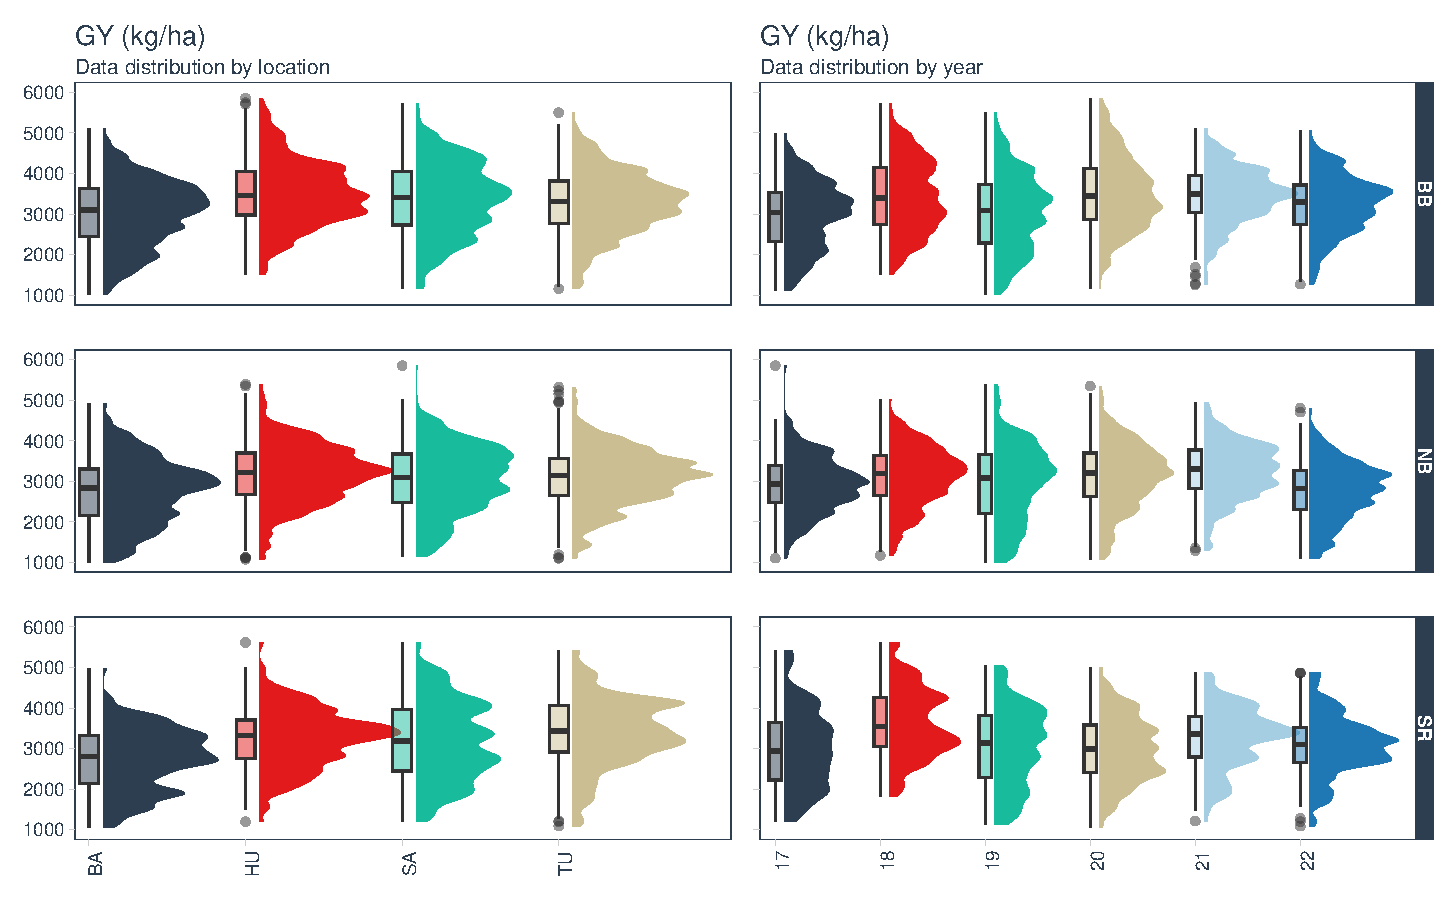
\includegraphics[width=1\linewidth]{figures/Box plot_raw data-1} \end{center}

\hypertarget{bb}{%
\paragraph{BB}\label{bb}}

\begin{Shaded}
\begin{Highlighting}[]
\NormalTok{data\_beans\_plotBB}\OtherTok{\textless{}{-}} \FunctionTok{droplevels}\NormalTok{(}\FunctionTok{subset}\NormalTok{(data\_beans, mkt}\SpecialCharTok{==}\StringTok{"BB"}\NormalTok{))}

\NormalTok{stats\_results\_BB}\OtherTok{\textless{}{-}} \FunctionTok{ggbetweenstats}\NormalTok{(}\AttributeTok{data=}\NormalTok{data\_beans\_plotBB, }\AttributeTok{x=}\NormalTok{ loc, }\AttributeTok{y=}\NormalTok{gy\_kg\_ha) }\SpecialCharTok{\%\textgreater{}\%} \FunctionTok{extract\_stats}\NormalTok{()   }
\CommentTok{\#print(stats\_results\_BB$pairwise\_comparisons\_data$p.value)}

\NormalTok{stats\_results\_BB2}\OtherTok{\textless{}{-}}\NormalTok{ stats\_results\_BB}\SpecialCharTok{$}\NormalTok{pairwise\_comparisons\_data }\SpecialCharTok{\%\textgreater{}\%} 
\NormalTok{dplyr}\SpecialCharTok{::}\FunctionTok{mutate}\NormalTok{(}\AttributeTok{groups =}\NormalTok{ purrr}\SpecialCharTok{::}\FunctionTok{pmap}\NormalTok{(}\AttributeTok{.l =} \FunctionTok{list}\NormalTok{(group1, group2), }\AttributeTok{.f =}\NormalTok{ c)) }\SpecialCharTok{\%\textgreater{}\%}
\NormalTok{  dplyr}\SpecialCharTok{::}\FunctionTok{arrange}\NormalTok{(group1)}\SpecialCharTok{\%\textgreater{}\%} 
  \FunctionTok{filter}\NormalTok{(p.value }\SpecialCharTok{\textless{}=} \FloatTok{0.05}\NormalTok{)}

\NormalTok{bb1}\OtherTok{\textless{}{-}} \FunctionTok{ggplot}\NormalTok{(}\AttributeTok{data=}\NormalTok{data\_beans\_plotBB, }\FunctionTok{aes}\NormalTok{(}\AttributeTok{x=}\FunctionTok{reorder}\NormalTok{(loc, }\SpecialCharTok{{-}}\NormalTok{gy\_kg\_ha), }\AttributeTok{y=}\NormalTok{gy\_kg\_ha, }\AttributeTok{fill=}\NormalTok{loc)) }\SpecialCharTok{+}
\NormalTok{  ggdist}\SpecialCharTok{::}\FunctionTok{stat\_halfeye}\NormalTok{(}
    \AttributeTok{adjust =} \FloatTok{0.5}\NormalTok{,}
    \AttributeTok{justification =} \SpecialCharTok{{-}}\FloatTok{0.1}\NormalTok{,}
    \AttributeTok{.width =} \DecValTok{0}\NormalTok{,}
    \AttributeTok{point\_colour =} \ConstantTok{NA}
\NormalTok{  ) }\SpecialCharTok{+}
  
  \FunctionTok{geom\_boxplot}\NormalTok{( }
    \AttributeTok{width =}\NormalTok{ .}\DecValTok{12}\NormalTok{,}
   \CommentTok{\# outlier.color = NA,}
    \AttributeTok{alpha =} \FloatTok{0.5}\NormalTok{)}\SpecialCharTok{+}
\NormalTok{  tidyquant}\SpecialCharTok{::}\FunctionTok{theme\_tq}\NormalTok{()}\SpecialCharTok{+}
  \CommentTok{\#facet\_grid("loc")+}
\NormalTok{  tidyquant}\SpecialCharTok{::}\FunctionTok{scale\_fill\_tq}\NormalTok{() }\SpecialCharTok{+}
  \FunctionTok{scale\_x\_discrete}\NormalTok{(}\AttributeTok{expand =} \FunctionTok{c}\NormalTok{(}\FloatTok{0.03}\NormalTok{,}\DecValTok{0}\NormalTok{)) }\SpecialCharTok{+}
  \FunctionTok{scale\_y\_continuous}\NormalTok{(}\AttributeTok{limits =} \FunctionTok{c}\NormalTok{(}\DecValTok{1000}\NormalTok{,}\DecValTok{10000}\NormalTok{), }\AttributeTok{breaks =} \FunctionTok{seq}\NormalTok{(}\DecValTok{1000}\NormalTok{, }\DecValTok{10000}\NormalTok{, }\AttributeTok{by =} \DecValTok{1000}\NormalTok{)) }\SpecialCharTok{+}
  \FunctionTok{theme}\NormalTok{(}\AttributeTok{axis.text.x=}\FunctionTok{element\_blank}\NormalTok{(),}
        \AttributeTok{strip.text=}\FunctionTok{element\_blank}\NormalTok{(),}
        \AttributeTok{legend.position =} \StringTok{"none"}\NormalTok{,}
        \AttributeTok{panel.grid =} \FunctionTok{element\_blank}\NormalTok{())}\SpecialCharTok{+}
  \FunctionTok{labs}\NormalTok{(}\AttributeTok{title=}\StringTok{"GY (kg/ha)"}\NormalTok{, }
       \AttributeTok{subtitle=}\StringTok{"Data distribution by location"}\NormalTok{, }
       \AttributeTok{caption=}\ConstantTok{NULL}\NormalTok{, }\AttributeTok{x=}\ConstantTok{NULL}\NormalTok{, }\AttributeTok{y=}\StringTok{"BB"}\NormalTok{)}

\NormalTok{bb1}\OtherTok{\textless{}{-}}\NormalTok{bb1 }\SpecialCharTok{+}
\NormalTok{  ggsignif}\SpecialCharTok{::}\FunctionTok{geom\_signif}\NormalTok{(}
    \AttributeTok{comparisons      =}\NormalTok{ stats\_results\_BB2}\SpecialCharTok{$}\NormalTok{groups,}
    \AttributeTok{map\_signif\_level =} \ConstantTok{TRUE}\NormalTok{,}
    \AttributeTok{tip\_length       =} \FloatTok{0.01}\NormalTok{,}
    \AttributeTok{textsize         =} \FloatTok{2.7}\NormalTok{,}
    \AttributeTok{y\_position       =} \FunctionTok{c}\NormalTok{(}\DecValTok{5900}\NormalTok{, }\DecValTok{6700}\NormalTok{, }\DecValTok{7500}\NormalTok{,}\DecValTok{8300}\NormalTok{, }\DecValTok{9100}\NormalTok{),}
    \AttributeTok{annotations      =} \FunctionTok{as.character}\NormalTok{(stats\_results\_BB2}\SpecialCharTok{$}\NormalTok{expression),}
    \AttributeTok{test             =} \ConstantTok{NULL}\NormalTok{,}
    \AttributeTok{na.rm            =} \ConstantTok{TRUE}\NormalTok{,}
    \AttributeTok{parse            =} \ConstantTok{TRUE}
\NormalTok{  )}
\end{Highlighting}
\end{Shaded}

\begin{Shaded}
\begin{Highlighting}[]
\NormalTok{data\_beans\_plotBB}\OtherTok{\textless{}{-}} \FunctionTok{droplevels}\NormalTok{(}\FunctionTok{subset}\NormalTok{(data\_beans, mkt}\SpecialCharTok{==}\StringTok{"BB"}\NormalTok{))}

\NormalTok{stats\_results\_BB}\OtherTok{\textless{}{-}} \FunctionTok{ggbetweenstats}\NormalTok{(}\AttributeTok{data=}\NormalTok{data\_beans\_plotBB, }\AttributeTok{x=}\NormalTok{ year, }\AttributeTok{y=}\NormalTok{gy\_kg\_ha) }\SpecialCharTok{\%\textgreater{}\%} \FunctionTok{extract\_stats}\NormalTok{()   }
\CommentTok{\#print(stats\_results\_BB$pairwise\_comparisons\_data$p.value)}

\NormalTok{stats\_results\_BB3}\OtherTok{\textless{}{-}}\NormalTok{ stats\_results\_BB}\SpecialCharTok{$}\NormalTok{pairwise\_comparisons\_data }\SpecialCharTok{\%\textgreater{}\%} 
\NormalTok{dplyr}\SpecialCharTok{::}\FunctionTok{mutate}\NormalTok{(}\AttributeTok{groups =}\NormalTok{ purrr}\SpecialCharTok{::}\FunctionTok{pmap}\NormalTok{(}\AttributeTok{.l =} \FunctionTok{list}\NormalTok{(group1, group2), }\AttributeTok{.f =}\NormalTok{ c)) }\SpecialCharTok{\%\textgreater{}\%}
\NormalTok{  dplyr}\SpecialCharTok{::}\FunctionTok{arrange}\NormalTok{(group1) }\SpecialCharTok{\%\textgreater{}\%} 
  \FunctionTok{filter}\NormalTok{(p.value }\SpecialCharTok{\textless{}=} \FloatTok{0.05}\NormalTok{)}

\NormalTok{bb2}\OtherTok{\textless{}{-}} \FunctionTok{ggplot}\NormalTok{(}\AttributeTok{data=}\NormalTok{data\_beans\_plotBB, }\FunctionTok{aes}\NormalTok{(}\AttributeTok{x=}\FunctionTok{reorder}\NormalTok{(year, }\SpecialCharTok{{-}}\NormalTok{gy\_kg\_ha), }\AttributeTok{y=}\NormalTok{gy\_kg\_ha, }\AttributeTok{fill=}\NormalTok{year)) }\SpecialCharTok{+}
\NormalTok{  ggdist}\SpecialCharTok{::}\FunctionTok{stat\_halfeye}\NormalTok{(}
    \AttributeTok{adjust =} \FloatTok{0.5}\NormalTok{,}
    \AttributeTok{justification =} \SpecialCharTok{{-}}\FloatTok{0.1}\NormalTok{,}
    \AttributeTok{.width =} \DecValTok{0}\NormalTok{,}
    \AttributeTok{point\_colour =} \ConstantTok{NA}
\NormalTok{  ) }\SpecialCharTok{+}
  
  \FunctionTok{geom\_boxplot}\NormalTok{( }
    \AttributeTok{width =}\NormalTok{ .}\DecValTok{12}\NormalTok{,}
   \CommentTok{\# outlier.color = NA,}
    \AttributeTok{alpha =} \FloatTok{0.5}\NormalTok{)}\SpecialCharTok{+}
\NormalTok{  tidyquant}\SpecialCharTok{::}\FunctionTok{theme\_tq}\NormalTok{()}\SpecialCharTok{+}
  \CommentTok{\#facet\_grid("loc")+}
\NormalTok{  tidyquant}\SpecialCharTok{::}\FunctionTok{scale\_fill\_tq}\NormalTok{() }\SpecialCharTok{+}
  \FunctionTok{scale\_x\_discrete}\NormalTok{(}\AttributeTok{expand =} \FunctionTok{c}\NormalTok{(}\FloatTok{0.03}\NormalTok{,}\DecValTok{0}\NormalTok{)) }\SpecialCharTok{+}
  \FunctionTok{scale\_y\_continuous}\NormalTok{(}\AttributeTok{limits =} \FunctionTok{c}\NormalTok{(}\DecValTok{1000}\NormalTok{,}\DecValTok{10000}\NormalTok{), }\AttributeTok{breaks =} \FunctionTok{seq}\NormalTok{(}\DecValTok{1000}\NormalTok{, }\DecValTok{10000}\NormalTok{, }\AttributeTok{by =} \DecValTok{1000}\NormalTok{)) }\SpecialCharTok{+}
  \FunctionTok{theme}\NormalTok{(}\AttributeTok{axis.text.x=}\FunctionTok{element\_blank}\NormalTok{(),}
        \AttributeTok{strip.text=}\FunctionTok{element\_blank}\NormalTok{(),}
        \AttributeTok{legend.position =} \StringTok{"none"}\NormalTok{,}
        \AttributeTok{panel.grid =} \FunctionTok{element\_blank}\NormalTok{())}\SpecialCharTok{+}
  \FunctionTok{labs}\NormalTok{(}\AttributeTok{title=}\StringTok{"GY (kg/ha)"}\NormalTok{, }
       \AttributeTok{subtitle=}\StringTok{"Data distribution by year"}\NormalTok{, }
       \AttributeTok{caption=}\ConstantTok{NULL}\NormalTok{, }\AttributeTok{x=}\ConstantTok{NULL}\NormalTok{, }\AttributeTok{y=}\ConstantTok{NULL}\NormalTok{)}


\NormalTok{bb2}\OtherTok{\textless{}{-}}\NormalTok{bb2 }\SpecialCharTok{+}
\NormalTok{  ggsignif}\SpecialCharTok{::}\FunctionTok{geom\_signif}\NormalTok{(}
    \AttributeTok{comparisons      =}\NormalTok{ stats\_results\_BB3}\SpecialCharTok{$}\NormalTok{groups,}
    \AttributeTok{map\_signif\_level =} \ConstantTok{TRUE}\NormalTok{,}
    \AttributeTok{tip\_length       =} \FloatTok{0.01}\NormalTok{,}
    \AttributeTok{textsize         =} \FloatTok{2.7}\NormalTok{,}
    \AttributeTok{y\_position       =} \FunctionTok{c}\NormalTok{(}\DecValTok{5900}\NormalTok{, }\DecValTok{6300}\NormalTok{, }\DecValTok{6700}\NormalTok{,}\DecValTok{7100}\NormalTok{, }\DecValTok{7400}\NormalTok{, }\DecValTok{7800}\NormalTok{,}\DecValTok{8200}\NormalTok{, }\DecValTok{8600}\NormalTok{, }\DecValTok{9000}\NormalTok{, }\DecValTok{9400}\NormalTok{),}
    \AttributeTok{annotations      =} \FunctionTok{as.character}\NormalTok{(stats\_results\_BB3}\SpecialCharTok{$}\NormalTok{expression),}
    \AttributeTok{test             =} \ConstantTok{NULL}\NormalTok{,}
    \AttributeTok{na.rm            =} \ConstantTok{TRUE}\NormalTok{,}
    \AttributeTok{parse            =} \ConstantTok{TRUE}
\NormalTok{  )}
\end{Highlighting}
\end{Shaded}

\hypertarget{nb}{%
\paragraph{NB}\label{nb}}

\begin{Shaded}
\begin{Highlighting}[]
\NormalTok{data\_beans\_plotBB}\OtherTok{\textless{}{-}} \FunctionTok{droplevels}\NormalTok{(}\FunctionTok{subset}\NormalTok{(data\_beans, mkt}\SpecialCharTok{==}\StringTok{"NB"}\NormalTok{))}

\NormalTok{stats\_results\_BB}\OtherTok{\textless{}{-}} \FunctionTok{ggbetweenstats}\NormalTok{(}\AttributeTok{data=}\NormalTok{data\_beans\_plotBB, }\AttributeTok{x=}\NormalTok{ loc, }\AttributeTok{y=}\NormalTok{gy\_kg\_ha) }\SpecialCharTok{\%\textgreater{}\%} \FunctionTok{extract\_stats}\NormalTok{()   }
\CommentTok{\#print(stats\_results\_BB$pairwise\_comparisons\_data$p.value)}

\NormalTok{stats\_results\_BB2}\OtherTok{\textless{}{-}}\NormalTok{ stats\_results\_BB}\SpecialCharTok{$}\NormalTok{pairwise\_comparisons\_data }\SpecialCharTok{\%\textgreater{}\%} 
\NormalTok{dplyr}\SpecialCharTok{::}\FunctionTok{mutate}\NormalTok{(}\AttributeTok{groups =}\NormalTok{ purrr}\SpecialCharTok{::}\FunctionTok{pmap}\NormalTok{(}\AttributeTok{.l =} \FunctionTok{list}\NormalTok{(group1, group2), }\AttributeTok{.f =}\NormalTok{ c)) }\SpecialCharTok{\%\textgreater{}\%}
\NormalTok{  dplyr}\SpecialCharTok{::}\FunctionTok{arrange}\NormalTok{(group1)}\SpecialCharTok{\%\textgreater{}\%} 
  \FunctionTok{filter}\NormalTok{(p.value }\SpecialCharTok{\textless{}=} \FloatTok{0.05}\NormalTok{)}

\NormalTok{nb1}\OtherTok{\textless{}{-}} \FunctionTok{ggplot}\NormalTok{(}\AttributeTok{data=}\NormalTok{data\_beans\_plotBB, }\FunctionTok{aes}\NormalTok{(}\AttributeTok{x=}\FunctionTok{reorder}\NormalTok{(loc, }\SpecialCharTok{{-}}\NormalTok{gy\_kg\_ha), }\AttributeTok{y=}\NormalTok{gy\_kg\_ha, }\AttributeTok{fill=}\NormalTok{loc)) }\SpecialCharTok{+}
\NormalTok{  ggdist}\SpecialCharTok{::}\FunctionTok{stat\_halfeye}\NormalTok{(}
    \AttributeTok{adjust =} \FloatTok{0.5}\NormalTok{,}
    \AttributeTok{justification =} \SpecialCharTok{{-}}\FloatTok{0.1}\NormalTok{,}
    \AttributeTok{.width =} \DecValTok{0}\NormalTok{,}
    \AttributeTok{point\_colour =} \ConstantTok{NA}
\NormalTok{  ) }\SpecialCharTok{+}
  
  \FunctionTok{geom\_boxplot}\NormalTok{( }
    \AttributeTok{width =}\NormalTok{ .}\DecValTok{12}\NormalTok{,}
   \CommentTok{\# outlier.color = NA,}
    \AttributeTok{alpha =} \FloatTok{0.5}\NormalTok{)}\SpecialCharTok{+}
\NormalTok{  tidyquant}\SpecialCharTok{::}\FunctionTok{theme\_tq}\NormalTok{()}\SpecialCharTok{+}
  \CommentTok{\#facet\_grid("loc")+}
\NormalTok{  tidyquant}\SpecialCharTok{::}\FunctionTok{scale\_fill\_tq}\NormalTok{() }\SpecialCharTok{+}
  \FunctionTok{scale\_x\_discrete}\NormalTok{(}\AttributeTok{expand =} \FunctionTok{c}\NormalTok{(}\FloatTok{0.03}\NormalTok{,}\DecValTok{0}\NormalTok{)) }\SpecialCharTok{+}
  \FunctionTok{scale\_y\_continuous}\NormalTok{(}\AttributeTok{limits =} \FunctionTok{c}\NormalTok{(}\DecValTok{1000}\NormalTok{,}\DecValTok{10000}\NormalTok{), }\AttributeTok{breaks =} \FunctionTok{seq}\NormalTok{(}\DecValTok{1000}\NormalTok{, }\DecValTok{10000}\NormalTok{, }\AttributeTok{by =} \DecValTok{1000}\NormalTok{)) }\SpecialCharTok{+}
  \FunctionTok{theme}\NormalTok{(}\AttributeTok{axis.text.x=}\FunctionTok{element\_blank}\NormalTok{(),}
        \AttributeTok{strip.text=}\FunctionTok{element\_blank}\NormalTok{(),}
        \AttributeTok{legend.position =} \StringTok{"none"}\NormalTok{,}
        \AttributeTok{panel.grid =} \FunctionTok{element\_blank}\NormalTok{())}\SpecialCharTok{+}
  \FunctionTok{labs}\NormalTok{( }
       \AttributeTok{caption=}\ConstantTok{NULL}\NormalTok{, }\AttributeTok{x=}\ConstantTok{NULL}\NormalTok{, }\AttributeTok{y=}\StringTok{"NB"}\NormalTok{)}

\NormalTok{nb1}\OtherTok{\textless{}{-}}\NormalTok{nb1 }\SpecialCharTok{+}
\NormalTok{  ggsignif}\SpecialCharTok{::}\FunctionTok{geom\_signif}\NormalTok{(}
    \AttributeTok{comparisons      =}\NormalTok{ stats\_results\_BB2}\SpecialCharTok{$}\NormalTok{groups,}
    \AttributeTok{map\_signif\_level =} \ConstantTok{TRUE}\NormalTok{,}
    \AttributeTok{tip\_length       =} \FloatTok{0.01}\NormalTok{,}
    \AttributeTok{textsize         =} \FloatTok{2.7}\NormalTok{,}
    \AttributeTok{y\_position       =} \FunctionTok{c}\NormalTok{(}\DecValTok{5900}\NormalTok{, }\DecValTok{6700}\NormalTok{, }\DecValTok{7500}\NormalTok{,}\DecValTok{8300}\NormalTok{, }\DecValTok{9100}\NormalTok{),}
    \AttributeTok{annotations      =} \FunctionTok{as.character}\NormalTok{(stats\_results\_BB2}\SpecialCharTok{$}\NormalTok{expression),}
    \AttributeTok{test             =} \ConstantTok{NULL}\NormalTok{,}
    \AttributeTok{na.rm            =} \ConstantTok{TRUE}\NormalTok{,}
    \AttributeTok{parse            =} \ConstantTok{TRUE}
\NormalTok{  )}
\end{Highlighting}
\end{Shaded}

\begin{Shaded}
\begin{Highlighting}[]
\NormalTok{data\_beans\_plotBB}\OtherTok{\textless{}{-}} \FunctionTok{droplevels}\NormalTok{(}\FunctionTok{subset}\NormalTok{(data\_beans, mkt}\SpecialCharTok{==}\StringTok{"NB"}\NormalTok{))}

\NormalTok{stats\_results\_BB}\OtherTok{\textless{}{-}} \FunctionTok{ggbetweenstats}\NormalTok{(}\AttributeTok{data=}\NormalTok{data\_beans\_plotBB, }\AttributeTok{x=}\NormalTok{ year, }\AttributeTok{y=}\NormalTok{gy\_kg\_ha) }\SpecialCharTok{\%\textgreater{}\%} \FunctionTok{extract\_stats}\NormalTok{()   }
\CommentTok{\#print(stats\_results\_BB$pairwise\_comparisons\_data$p.value)}

\NormalTok{stats\_results\_BB3}\OtherTok{\textless{}{-}}\NormalTok{ stats\_results\_BB}\SpecialCharTok{$}\NormalTok{pairwise\_comparisons\_data }\SpecialCharTok{\%\textgreater{}\%} 
\NormalTok{dplyr}\SpecialCharTok{::}\FunctionTok{mutate}\NormalTok{(}\AttributeTok{groups =}\NormalTok{ purrr}\SpecialCharTok{::}\FunctionTok{pmap}\NormalTok{(}\AttributeTok{.l =} \FunctionTok{list}\NormalTok{(group1, group2), }\AttributeTok{.f =}\NormalTok{ c)) }\SpecialCharTok{\%\textgreater{}\%}
\NormalTok{  dplyr}\SpecialCharTok{::}\FunctionTok{arrange}\NormalTok{(group1) }\SpecialCharTok{\%\textgreater{}\%} 
  \FunctionTok{filter}\NormalTok{(p.value }\SpecialCharTok{\textless{}=} \FloatTok{0.05}\NormalTok{)}

\NormalTok{nb2}\OtherTok{\textless{}{-}} \FunctionTok{ggplot}\NormalTok{(}\AttributeTok{data=}\NormalTok{data\_beans\_plotBB, }\FunctionTok{aes}\NormalTok{(}\AttributeTok{x=}\FunctionTok{reorder}\NormalTok{(year, }\SpecialCharTok{{-}}\NormalTok{gy\_kg\_ha), }\AttributeTok{y=}\NormalTok{gy\_kg\_ha, }\AttributeTok{fill=}\NormalTok{year)) }\SpecialCharTok{+}
\NormalTok{  ggdist}\SpecialCharTok{::}\FunctionTok{stat\_halfeye}\NormalTok{(}
    \AttributeTok{adjust =} \FloatTok{0.5}\NormalTok{,}
    \AttributeTok{justification =} \SpecialCharTok{{-}}\FloatTok{0.1}\NormalTok{,}
    \AttributeTok{.width =} \DecValTok{0}\NormalTok{,}
    \AttributeTok{point\_colour =} \ConstantTok{NA}
\NormalTok{  ) }\SpecialCharTok{+}
  
  \FunctionTok{geom\_boxplot}\NormalTok{( }
    \AttributeTok{width =}\NormalTok{ .}\DecValTok{12}\NormalTok{,}
   \CommentTok{\# outlier.color = NA,}
    \AttributeTok{alpha =} \FloatTok{0.5}\NormalTok{)}\SpecialCharTok{+}
\NormalTok{  tidyquant}\SpecialCharTok{::}\FunctionTok{theme\_tq}\NormalTok{()}\SpecialCharTok{+}
  \CommentTok{\#facet\_grid("loc")+}
\NormalTok{  tidyquant}\SpecialCharTok{::}\FunctionTok{scale\_fill\_tq}\NormalTok{() }\SpecialCharTok{+}
  \FunctionTok{scale\_x\_discrete}\NormalTok{(}\AttributeTok{expand =} \FunctionTok{c}\NormalTok{(}\FloatTok{0.03}\NormalTok{,}\DecValTok{0}\NormalTok{)) }\SpecialCharTok{+}
  \FunctionTok{scale\_y\_continuous}\NormalTok{(}\AttributeTok{limits =} \FunctionTok{c}\NormalTok{(}\DecValTok{1000}\NormalTok{,}\DecValTok{10000}\NormalTok{), }\AttributeTok{breaks =} \FunctionTok{seq}\NormalTok{(}\DecValTok{1000}\NormalTok{, }\DecValTok{10000}\NormalTok{, }\AttributeTok{by =} \DecValTok{1000}\NormalTok{)) }\SpecialCharTok{+}
  \FunctionTok{theme}\NormalTok{(}\AttributeTok{axis.text.x=}\FunctionTok{element\_blank}\NormalTok{(),}
        \AttributeTok{strip.text=}\FunctionTok{element\_blank}\NormalTok{(),}
        \AttributeTok{legend.position =} \StringTok{"none"}\NormalTok{,}
        \AttributeTok{panel.grid =} \FunctionTok{element\_blank}\NormalTok{())}\SpecialCharTok{+}
  \FunctionTok{labs}\NormalTok{( }
       \AttributeTok{caption=}\ConstantTok{NULL}\NormalTok{, }\AttributeTok{x=}\ConstantTok{NULL}\NormalTok{, }\AttributeTok{y=}\ConstantTok{NULL}\NormalTok{)}


\NormalTok{nb2}\OtherTok{\textless{}{-}}\NormalTok{nb2 }\SpecialCharTok{+}
\NormalTok{  ggsignif}\SpecialCharTok{::}\FunctionTok{geom\_signif}\NormalTok{(}
    \AttributeTok{comparisons      =}\NormalTok{ stats\_results\_BB3}\SpecialCharTok{$}\NormalTok{groups,}
    \AttributeTok{map\_signif\_level =} \ConstantTok{TRUE}\NormalTok{,}
    \AttributeTok{tip\_length       =} \FloatTok{0.01}\NormalTok{,}
    \AttributeTok{textsize         =} \FloatTok{2.7}\NormalTok{,}
    \AttributeTok{y\_position       =} \FunctionTok{c}\NormalTok{(}\DecValTok{5900}\NormalTok{, }\DecValTok{6300}\NormalTok{, }\DecValTok{6700}\NormalTok{,}\DecValTok{7100}\NormalTok{, }\DecValTok{7400}\NormalTok{, }\DecValTok{7800}\NormalTok{,}\DecValTok{8200}\NormalTok{, }\DecValTok{8600}\NormalTok{, }\DecValTok{9000}\NormalTok{, }\DecValTok{9400}\NormalTok{),}
    \AttributeTok{annotations      =} \FunctionTok{as.character}\NormalTok{(stats\_results\_BB3}\SpecialCharTok{$}\NormalTok{expression),}
    \AttributeTok{test             =} \ConstantTok{NULL}\NormalTok{,}
    \AttributeTok{na.rm            =} \ConstantTok{TRUE}\NormalTok{,}
    \AttributeTok{parse            =} \ConstantTok{TRUE}
\NormalTok{  )}
\end{Highlighting}
\end{Shaded}

\hypertarget{sr}{%
\paragraph{SR}\label{sr}}

\begin{Shaded}
\begin{Highlighting}[]
\NormalTok{data\_beans\_plotBB}\OtherTok{\textless{}{-}} \FunctionTok{droplevels}\NormalTok{(}\FunctionTok{subset}\NormalTok{(data\_beans, mkt}\SpecialCharTok{==}\StringTok{"SR"}\NormalTok{))}

\NormalTok{stats\_results\_BB}\OtherTok{\textless{}{-}} \FunctionTok{ggbetweenstats}\NormalTok{(}\AttributeTok{data=}\NormalTok{data\_beans\_plotBB, }\AttributeTok{x=}\NormalTok{ loc, }\AttributeTok{y=}\NormalTok{gy\_kg\_ha) }\SpecialCharTok{\%\textgreater{}\%} \FunctionTok{extract\_stats}\NormalTok{()   }
\CommentTok{\#print(stats\_results\_BB$pairwise\_comparisons\_data$p.value)}

\NormalTok{stats\_results\_BB2}\OtherTok{\textless{}{-}}\NormalTok{ stats\_results\_BB}\SpecialCharTok{$}\NormalTok{pairwise\_comparisons\_data }\SpecialCharTok{\%\textgreater{}\%} 
\NormalTok{dplyr}\SpecialCharTok{::}\FunctionTok{mutate}\NormalTok{(}\AttributeTok{groups =}\NormalTok{ purrr}\SpecialCharTok{::}\FunctionTok{pmap}\NormalTok{(}\AttributeTok{.l =} \FunctionTok{list}\NormalTok{(group1, group2), }\AttributeTok{.f =}\NormalTok{ c)) }\SpecialCharTok{\%\textgreater{}\%}
\NormalTok{  dplyr}\SpecialCharTok{::}\FunctionTok{arrange}\NormalTok{(group1)}\SpecialCharTok{\%\textgreater{}\%} 
  \FunctionTok{filter}\NormalTok{(p.value }\SpecialCharTok{\textless{}=} \FloatTok{0.05}\NormalTok{)}

\NormalTok{sr1}\OtherTok{\textless{}{-}} \FunctionTok{ggplot}\NormalTok{(}\AttributeTok{data=}\NormalTok{data\_beans\_plotBB, }\FunctionTok{aes}\NormalTok{(}\AttributeTok{x=}\FunctionTok{reorder}\NormalTok{(loc, }\SpecialCharTok{{-}}\NormalTok{gy\_kg\_ha), }\AttributeTok{y=}\NormalTok{gy\_kg\_ha, }\AttributeTok{fill=}\NormalTok{loc)) }\SpecialCharTok{+}
\NormalTok{  ggdist}\SpecialCharTok{::}\FunctionTok{stat\_halfeye}\NormalTok{(}
    \AttributeTok{adjust =} \FloatTok{0.5}\NormalTok{,}
    \AttributeTok{justification =} \SpecialCharTok{{-}}\FloatTok{0.1}\NormalTok{,}
    \AttributeTok{.width =} \DecValTok{0}\NormalTok{,}
    \AttributeTok{point\_colour =} \ConstantTok{NA}
\NormalTok{  ) }\SpecialCharTok{+}
  
  \FunctionTok{geom\_boxplot}\NormalTok{( }
    \AttributeTok{width =}\NormalTok{ .}\DecValTok{12}\NormalTok{,}
   \CommentTok{\# outlier.color = NA,}
    \AttributeTok{alpha =} \FloatTok{0.5}\NormalTok{)}\SpecialCharTok{+}
\NormalTok{  tidyquant}\SpecialCharTok{::}\FunctionTok{theme\_tq}\NormalTok{()}\SpecialCharTok{+}
  \CommentTok{\#facet\_grid("loc")+}
\NormalTok{  tidyquant}\SpecialCharTok{::}\FunctionTok{scale\_fill\_tq}\NormalTok{() }\SpecialCharTok{+}
  \FunctionTok{scale\_x\_discrete}\NormalTok{(}\AttributeTok{expand =} \FunctionTok{c}\NormalTok{(}\FloatTok{0.03}\NormalTok{,}\DecValTok{0}\NormalTok{)) }\SpecialCharTok{+}
  \FunctionTok{scale\_y\_continuous}\NormalTok{(}\AttributeTok{limits =} \FunctionTok{c}\NormalTok{(}\DecValTok{1000}\NormalTok{,}\DecValTok{10000}\NormalTok{), }\AttributeTok{breaks =} \FunctionTok{seq}\NormalTok{(}\DecValTok{1000}\NormalTok{, }\DecValTok{10000}\NormalTok{, }\AttributeTok{by =} \DecValTok{1000}\NormalTok{)) }\SpecialCharTok{+}
  \FunctionTok{theme}\NormalTok{(}
        \AttributeTok{strip.text=}\FunctionTok{element\_blank}\NormalTok{(),}
        \AttributeTok{legend.position =} \StringTok{"none"}\NormalTok{,}
        \AttributeTok{panel.grid =} \FunctionTok{element\_blank}\NormalTok{())}\SpecialCharTok{+}
  \FunctionTok{labs}\NormalTok{(}
       \AttributeTok{caption=}\ConstantTok{NULL}\NormalTok{, }\AttributeTok{x=}\StringTok{"Locations"}\NormalTok{, }\AttributeTok{y=}\StringTok{"SR"}\NormalTok{)}

\NormalTok{sr1}\OtherTok{\textless{}{-}}\NormalTok{sr1 }\SpecialCharTok{+}
\NormalTok{  ggsignif}\SpecialCharTok{::}\FunctionTok{geom\_signif}\NormalTok{(}
    \AttributeTok{comparisons      =}\NormalTok{ stats\_results\_BB2}\SpecialCharTok{$}\NormalTok{groups,}
    \AttributeTok{map\_signif\_level =} \ConstantTok{TRUE}\NormalTok{,}
    \AttributeTok{tip\_length       =} \FloatTok{0.01}\NormalTok{,}
    \AttributeTok{textsize         =} \FloatTok{2.7}\NormalTok{,}
    \AttributeTok{y\_position       =} \FunctionTok{c}\NormalTok{(}\DecValTok{5900}\NormalTok{, }\DecValTok{6700}\NormalTok{, }\DecValTok{7500}\NormalTok{,}\DecValTok{8300}\NormalTok{, }\DecValTok{9100}\NormalTok{),}
    \AttributeTok{annotations      =} \FunctionTok{as.character}\NormalTok{(stats\_results\_BB2}\SpecialCharTok{$}\NormalTok{expression),}
    \AttributeTok{test             =} \ConstantTok{NULL}\NormalTok{,}
    \AttributeTok{na.rm            =} \ConstantTok{TRUE}\NormalTok{,}
    \AttributeTok{parse            =} \ConstantTok{TRUE}
\NormalTok{  )}
\end{Highlighting}
\end{Shaded}

\begin{Shaded}
\begin{Highlighting}[]
\NormalTok{data\_beans\_plotBB}\OtherTok{\textless{}{-}} \FunctionTok{droplevels}\NormalTok{(}\FunctionTok{subset}\NormalTok{(data\_beans, mkt}\SpecialCharTok{==}\StringTok{"SR"}\NormalTok{))}

\NormalTok{stats\_results\_BB}\OtherTok{\textless{}{-}} \FunctionTok{ggbetweenstats}\NormalTok{(}\AttributeTok{data=}\NormalTok{data\_beans\_plotBB, }\AttributeTok{x=}\NormalTok{ year, }\AttributeTok{y=}\NormalTok{gy\_kg\_ha) }\SpecialCharTok{\%\textgreater{}\%} \FunctionTok{extract\_stats}\NormalTok{()   }
\CommentTok{\#print(stats\_results\_BB$pairwise\_comparisons\_data$p.value)}

\NormalTok{stats\_results\_BB3}\OtherTok{\textless{}{-}}\NormalTok{ stats\_results\_BB}\SpecialCharTok{$}\NormalTok{pairwise\_comparisons\_data }\SpecialCharTok{\%\textgreater{}\%} 
\NormalTok{dplyr}\SpecialCharTok{::}\FunctionTok{mutate}\NormalTok{(}\AttributeTok{groups =}\NormalTok{ purrr}\SpecialCharTok{::}\FunctionTok{pmap}\NormalTok{(}\AttributeTok{.l =} \FunctionTok{list}\NormalTok{(group1, group2), }\AttributeTok{.f =}\NormalTok{ c)) }\SpecialCharTok{\%\textgreater{}\%}
\NormalTok{  dplyr}\SpecialCharTok{::}\FunctionTok{arrange}\NormalTok{(group1) }\SpecialCharTok{\%\textgreater{}\%} 
  \FunctionTok{filter}\NormalTok{(p.value }\SpecialCharTok{\textless{}=} \FloatTok{0.05}\NormalTok{)}

\NormalTok{sr2}\OtherTok{\textless{}{-}} \FunctionTok{ggplot}\NormalTok{(}\AttributeTok{data=}\NormalTok{data\_beans\_plotBB, }\FunctionTok{aes}\NormalTok{(}\AttributeTok{x=}\FunctionTok{reorder}\NormalTok{(year, }\SpecialCharTok{{-}}\NormalTok{gy\_kg\_ha), }\AttributeTok{y=}\NormalTok{gy\_kg\_ha, }\AttributeTok{fill=}\NormalTok{year)) }\SpecialCharTok{+}
\NormalTok{  ggdist}\SpecialCharTok{::}\FunctionTok{stat\_halfeye}\NormalTok{(}
    \AttributeTok{adjust =} \FloatTok{0.5}\NormalTok{,}
    \AttributeTok{justification =} \SpecialCharTok{{-}}\FloatTok{0.1}\NormalTok{,}
    \AttributeTok{.width =} \DecValTok{0}\NormalTok{,}
    \AttributeTok{point\_colour =} \ConstantTok{NA}
\NormalTok{  ) }\SpecialCharTok{+}
  
  \FunctionTok{geom\_boxplot}\NormalTok{( }
    \AttributeTok{width =}\NormalTok{ .}\DecValTok{12}\NormalTok{,}
   \CommentTok{\# outlier.color = NA,}
    \AttributeTok{alpha =} \FloatTok{0.5}\NormalTok{)}\SpecialCharTok{+}
\NormalTok{  tidyquant}\SpecialCharTok{::}\FunctionTok{theme\_tq}\NormalTok{()}\SpecialCharTok{+}
  \CommentTok{\#facet\_grid("loc")+}
\NormalTok{  tidyquant}\SpecialCharTok{::}\FunctionTok{scale\_fill\_tq}\NormalTok{() }\SpecialCharTok{+}
  \FunctionTok{scale\_x\_discrete}\NormalTok{(}\AttributeTok{expand =} \FunctionTok{c}\NormalTok{(}\FloatTok{0.03}\NormalTok{,}\DecValTok{0}\NormalTok{)) }\SpecialCharTok{+}
  \FunctionTok{scale\_y\_continuous}\NormalTok{(}\AttributeTok{limits =} \FunctionTok{c}\NormalTok{(}\DecValTok{1000}\NormalTok{,}\DecValTok{10000}\NormalTok{), }\AttributeTok{breaks =} \FunctionTok{seq}\NormalTok{(}\DecValTok{1000}\NormalTok{, }\DecValTok{10000}\NormalTok{, }\AttributeTok{by =} \DecValTok{1000}\NormalTok{)) }\SpecialCharTok{+}
  \FunctionTok{theme}\NormalTok{(}
        \AttributeTok{strip.text=}\FunctionTok{element\_blank}\NormalTok{(),}
        \AttributeTok{legend.position =} \StringTok{"none"}\NormalTok{,}
        \AttributeTok{panel.grid =} \FunctionTok{element\_blank}\NormalTok{())}\SpecialCharTok{+}
  \FunctionTok{labs}\NormalTok{(}
       \AttributeTok{caption=}\ConstantTok{NULL}\NormalTok{, }\AttributeTok{y=}\ConstantTok{NULL}\NormalTok{, }\AttributeTok{x=}\StringTok{"Years"}\NormalTok{)}


\NormalTok{sr2}\OtherTok{\textless{}{-}}\NormalTok{ sr2 }\SpecialCharTok{+}
\NormalTok{  ggsignif}\SpecialCharTok{::}\FunctionTok{geom\_signif}\NormalTok{(}
    \AttributeTok{comparisons      =}\NormalTok{ stats\_results\_BB3}\SpecialCharTok{$}\NormalTok{groups,}
    \AttributeTok{map\_signif\_level =} \ConstantTok{TRUE}\NormalTok{,}
    \AttributeTok{tip\_length       =} \FloatTok{0.01}\NormalTok{,}
    \AttributeTok{textsize         =} \FloatTok{2.7}\NormalTok{,}
    \AttributeTok{y\_position       =} \FunctionTok{c}\NormalTok{(}\DecValTok{5900}\NormalTok{, }\DecValTok{6500}\NormalTok{, }\DecValTok{7200}\NormalTok{,}\DecValTok{8000}\NormalTok{, }\DecValTok{8700}\NormalTok{, }\DecValTok{9500}\NormalTok{),}
    \AttributeTok{annotations      =} \FunctionTok{as.character}\NormalTok{(stats\_results\_BB3}\SpecialCharTok{$}\NormalTok{expression),}
    \AttributeTok{test             =} \ConstantTok{NULL}\NormalTok{,}
    \AttributeTok{na.rm            =} \ConstantTok{TRUE}\NormalTok{,}
    \AttributeTok{parse            =} \ConstantTok{TRUE}
\NormalTok{  )}
\end{Highlighting}
\end{Shaded}

Box plot distribution for each market class in this study across years
and locations.

\begin{Shaded}
\begin{Highlighting}[]
\FunctionTok{print}\NormalTok{(}\FunctionTok{arrange\_ggplot}\NormalTok{(bb1,bb2,}
\NormalTok{                     nb1,nb2,}
\NormalTok{                     sr1,sr2,}
                     \AttributeTok{nrow =} \DecValTok{3}\NormalTok{,}
                     \AttributeTok{ncol =} \DecValTok{2}\NormalTok{))}
\end{Highlighting}
\end{Shaded}

\begin{center}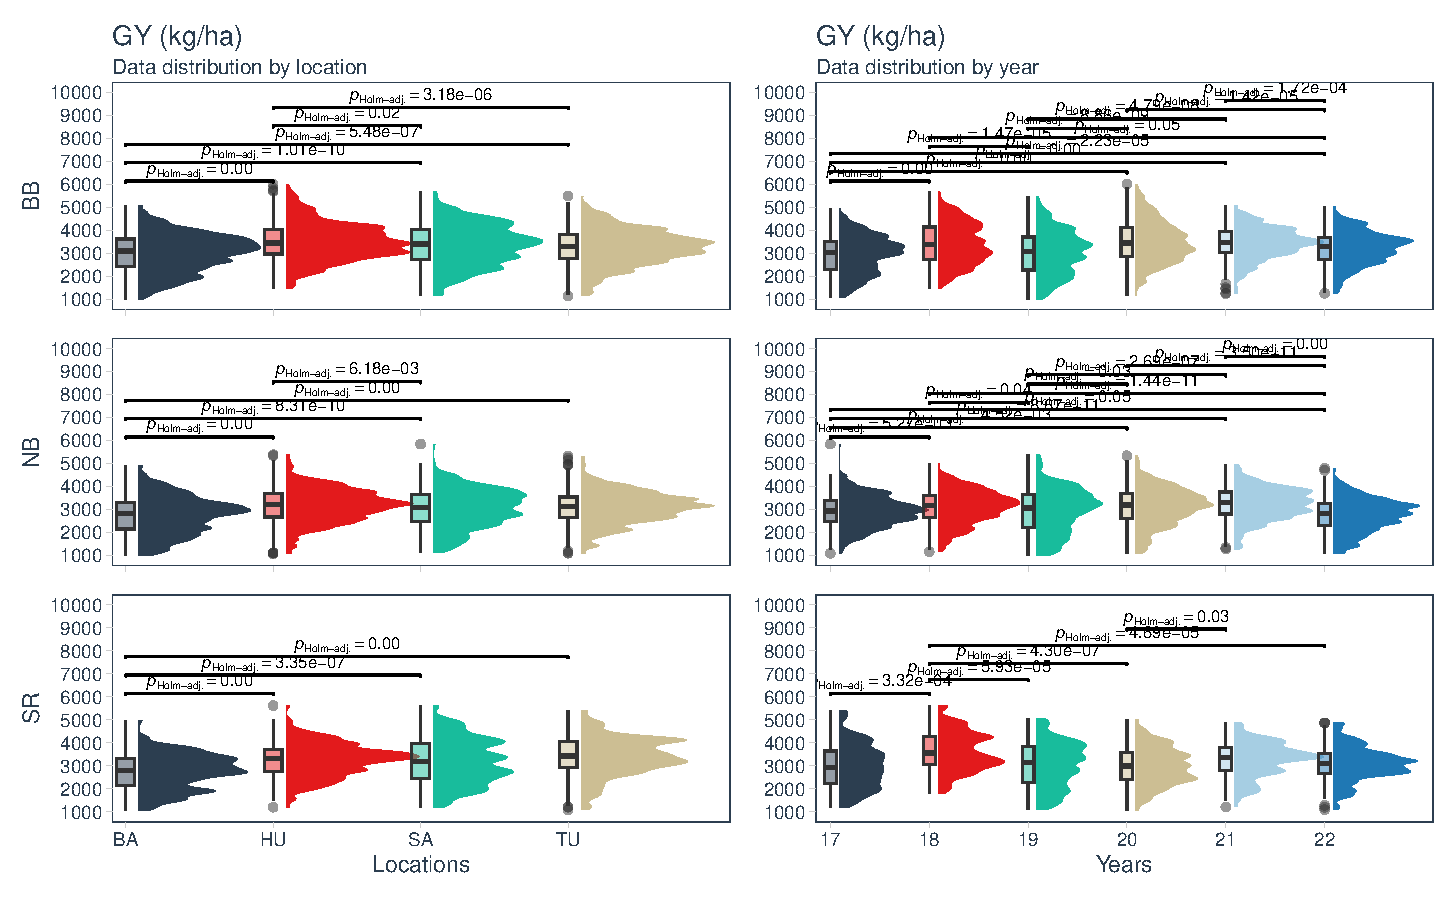
\includegraphics[width=1\linewidth]{figures/plot_Box complete final-1} \end{center}

\hypertarget{gei-comparisons-locyear---bb}{%
\subsubsection{GEI Comparisons (loc:year) -
BB}\label{gei-comparisons-locyear---bb}}

Box plots for between-subjects comparisons by locations using the R
package \texttt{ggstatsplot}.

\begin{itemize}
\tightlist
\item
  Combination analysis across all market classes (Comb\_MKT)
\item
  \textbf{Pairwise Games-Howell test used. Comparisons showing
  significant values only}
\end{itemize}

\begin{Shaded}
\begin{Highlighting}[]
\NormalTok{plotDM\_stats\_mkt\_loc\_all}\OtherTok{\textless{}{-}} \FunctionTok{grouped\_ggbetweenstats}\NormalTok{(}\AttributeTok{data=}\NormalTok{data\_beans, }\AttributeTok{x=}\NormalTok{ loc, }\AttributeTok{y=}\NormalTok{gy\_kg\_ha, }\AttributeTok{type =} \StringTok{"parametric"}\NormalTok{, }
                                                  \AttributeTok{bf.message =}\NormalTok{ F, }\AttributeTok{results.subtitle =}\NormalTok{ F,}
\AttributeTok{ylab=} \StringTok{"GY"}\NormalTok{, }\AttributeTok{xlab =} \StringTok{"Locations"}\NormalTok{, }\AttributeTok{plot.type =} \StringTok{"boxviolin"}\NormalTok{, }\AttributeTok{grouping.var =}\NormalTok{ year )}

\FunctionTok{print}\NormalTok{(plotDM\_stats\_mkt\_loc\_all)}
\end{Highlighting}
\end{Shaded}

\begin{center}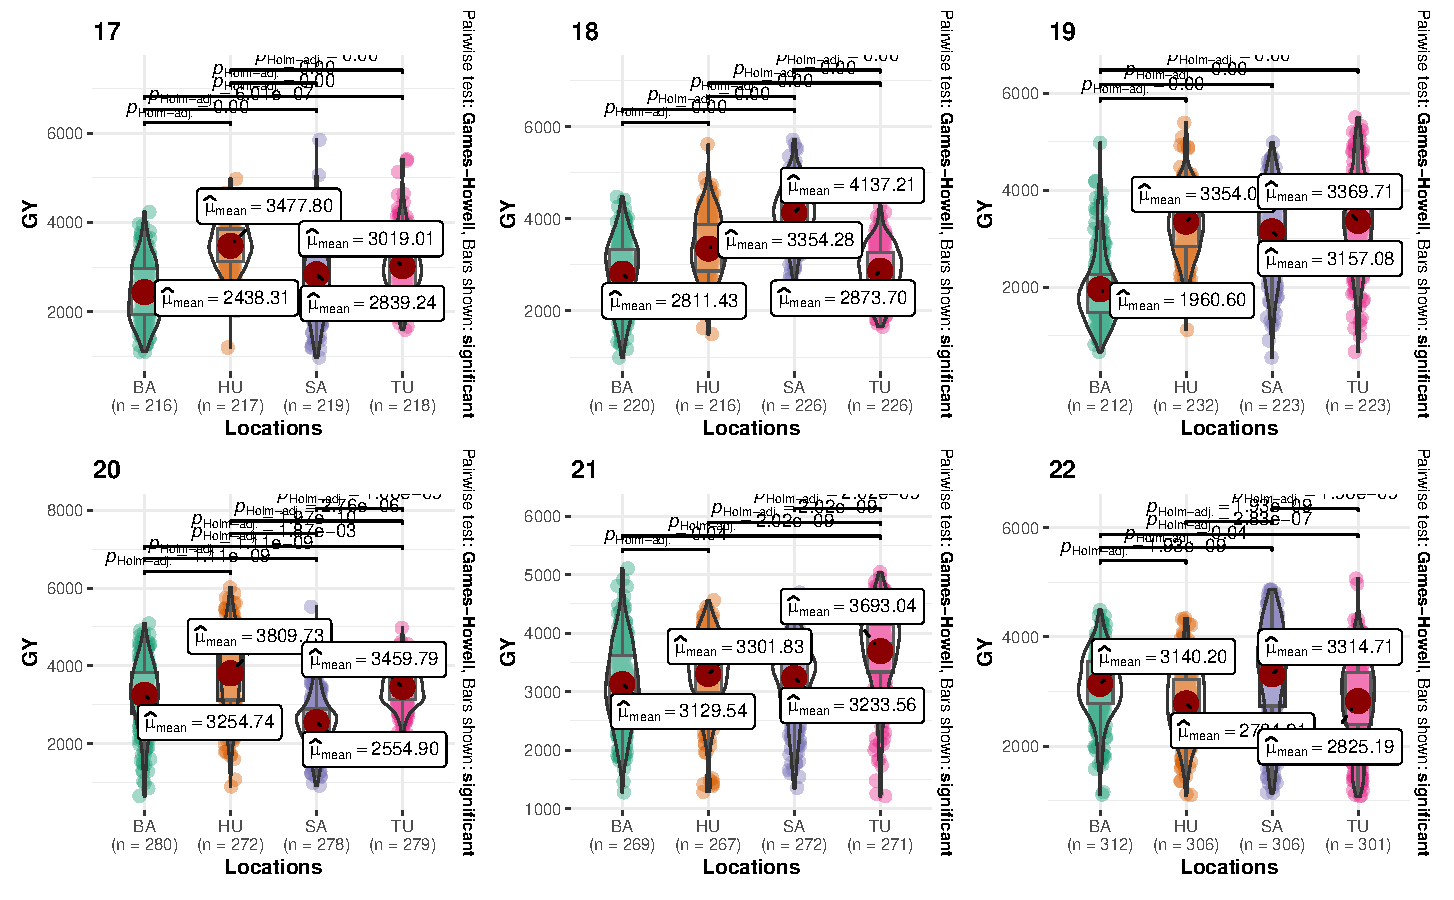
\includegraphics[width=1\linewidth]{figures/plot_ggstatsplot_desc_all_mkt-1} \end{center}

\begin{itemize}
\tightlist
\item
  Black beans (BB)
\item
  \textbf{Pairwise Games-Howell test used. Comparisons showing
  significant values only}
\end{itemize}

\begin{Shaded}
\begin{Highlighting}[]
\NormalTok{data\_beans\_plotBB}\OtherTok{\textless{}{-}} \FunctionTok{droplevels}\NormalTok{(}\FunctionTok{subset}\NormalTok{(data\_beans, mkt}\SpecialCharTok{==}\StringTok{"BB"}\NormalTok{))}

\NormalTok{plotDM\_stats\_mkt\_loc\_BB}\OtherTok{\textless{}{-}} \FunctionTok{grouped\_ggbetweenstats}\NormalTok{(}\AttributeTok{data=}\NormalTok{data\_beans\_plotBB, }\AttributeTok{x=}\NormalTok{ loc, }\AttributeTok{y=}\NormalTok{gy\_kg\_ha, }\AttributeTok{type =} \StringTok{"parametric"}\NormalTok{,  }\AttributeTok{bf.message =}\NormalTok{ F, }\AttributeTok{results.subtitle =}\NormalTok{ F, }
                              \AttributeTok{ylab=} \StringTok{"GY"}\NormalTok{, }\AttributeTok{xlab =} \StringTok{"Locations"}\NormalTok{,}
                              \AttributeTok{plot.type =} \StringTok{"boxviolin"}\NormalTok{, }\AttributeTok{grouping.var =}\NormalTok{ year ) }
\FunctionTok{print}\NormalTok{(plotDM\_stats\_mkt\_loc\_BB)}
\end{Highlighting}
\end{Shaded}

\begin{center}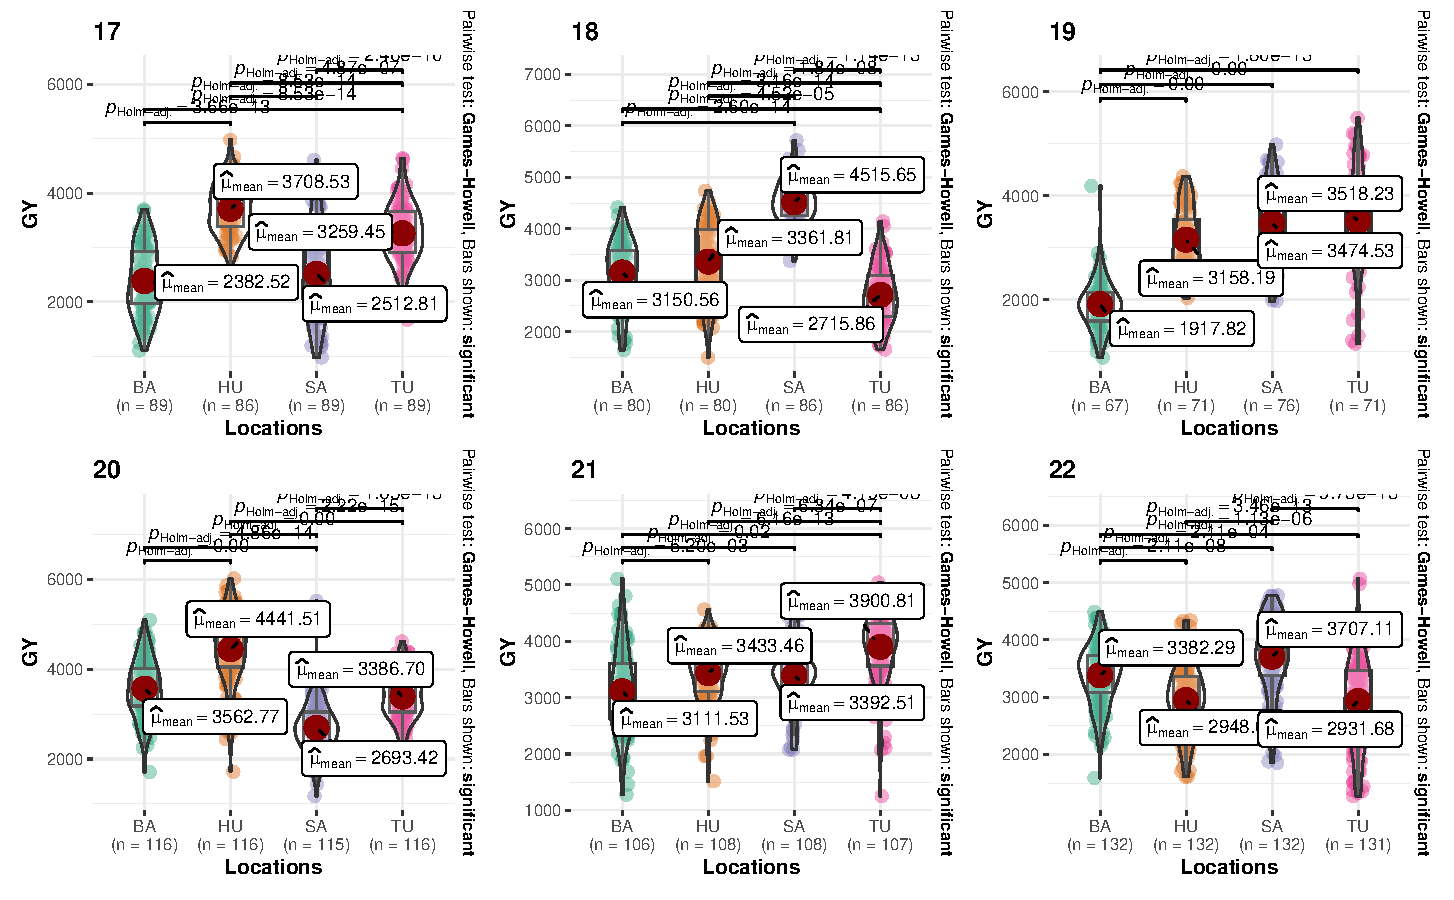
\includegraphics[width=1\linewidth]{figures/plot_ggstatsplot_desc_BB-1} \end{center}

\hypertarget{gei-comparisons-locyear---nb}{%
\subsubsection{GEI Comparisons (loc:year) -
NB}\label{gei-comparisons-locyear---nb}}

Box plots for between-subjects comparisons by locations using the R
package \texttt{ggstatsplot}. - Navy beans (NB) - \textbf{Pairwise
Games-Howell test used. Comparisons showing significant values only}

\begin{Shaded}
\begin{Highlighting}[]
\NormalTok{data\_beans\_plotNB}\OtherTok{\textless{}{-}} \FunctionTok{droplevels}\NormalTok{(}\FunctionTok{subset}\NormalTok{(data\_beans, mkt}\SpecialCharTok{==}\StringTok{"NB"}\NormalTok{))}

\NormalTok{plotDM\_stats\_mkt\_loc\_NB}\OtherTok{\textless{}{-}} \FunctionTok{grouped\_ggbetweenstats}\NormalTok{(}\AttributeTok{data=}\NormalTok{data\_beans\_plotNB, }\AttributeTok{x=}\NormalTok{ loc, }\AttributeTok{y=}\NormalTok{gy\_kg\_ha, }\AttributeTok{type =} \StringTok{"parametric"}\NormalTok{,  }\AttributeTok{bf.message =}\NormalTok{ F, }\AttributeTok{results.subtitle =}\NormalTok{ F, }
                              \AttributeTok{ylab=} \StringTok{"GY"}\NormalTok{, }\AttributeTok{xlab =} \StringTok{"Locations"}\NormalTok{,}
                              \AttributeTok{plot.type =} \StringTok{"boxviolin"}\NormalTok{, }\AttributeTok{grouping.var =}\NormalTok{ year ) }
\FunctionTok{print}\NormalTok{(plotDM\_stats\_mkt\_loc\_NB)}
\end{Highlighting}
\end{Shaded}

\begin{center}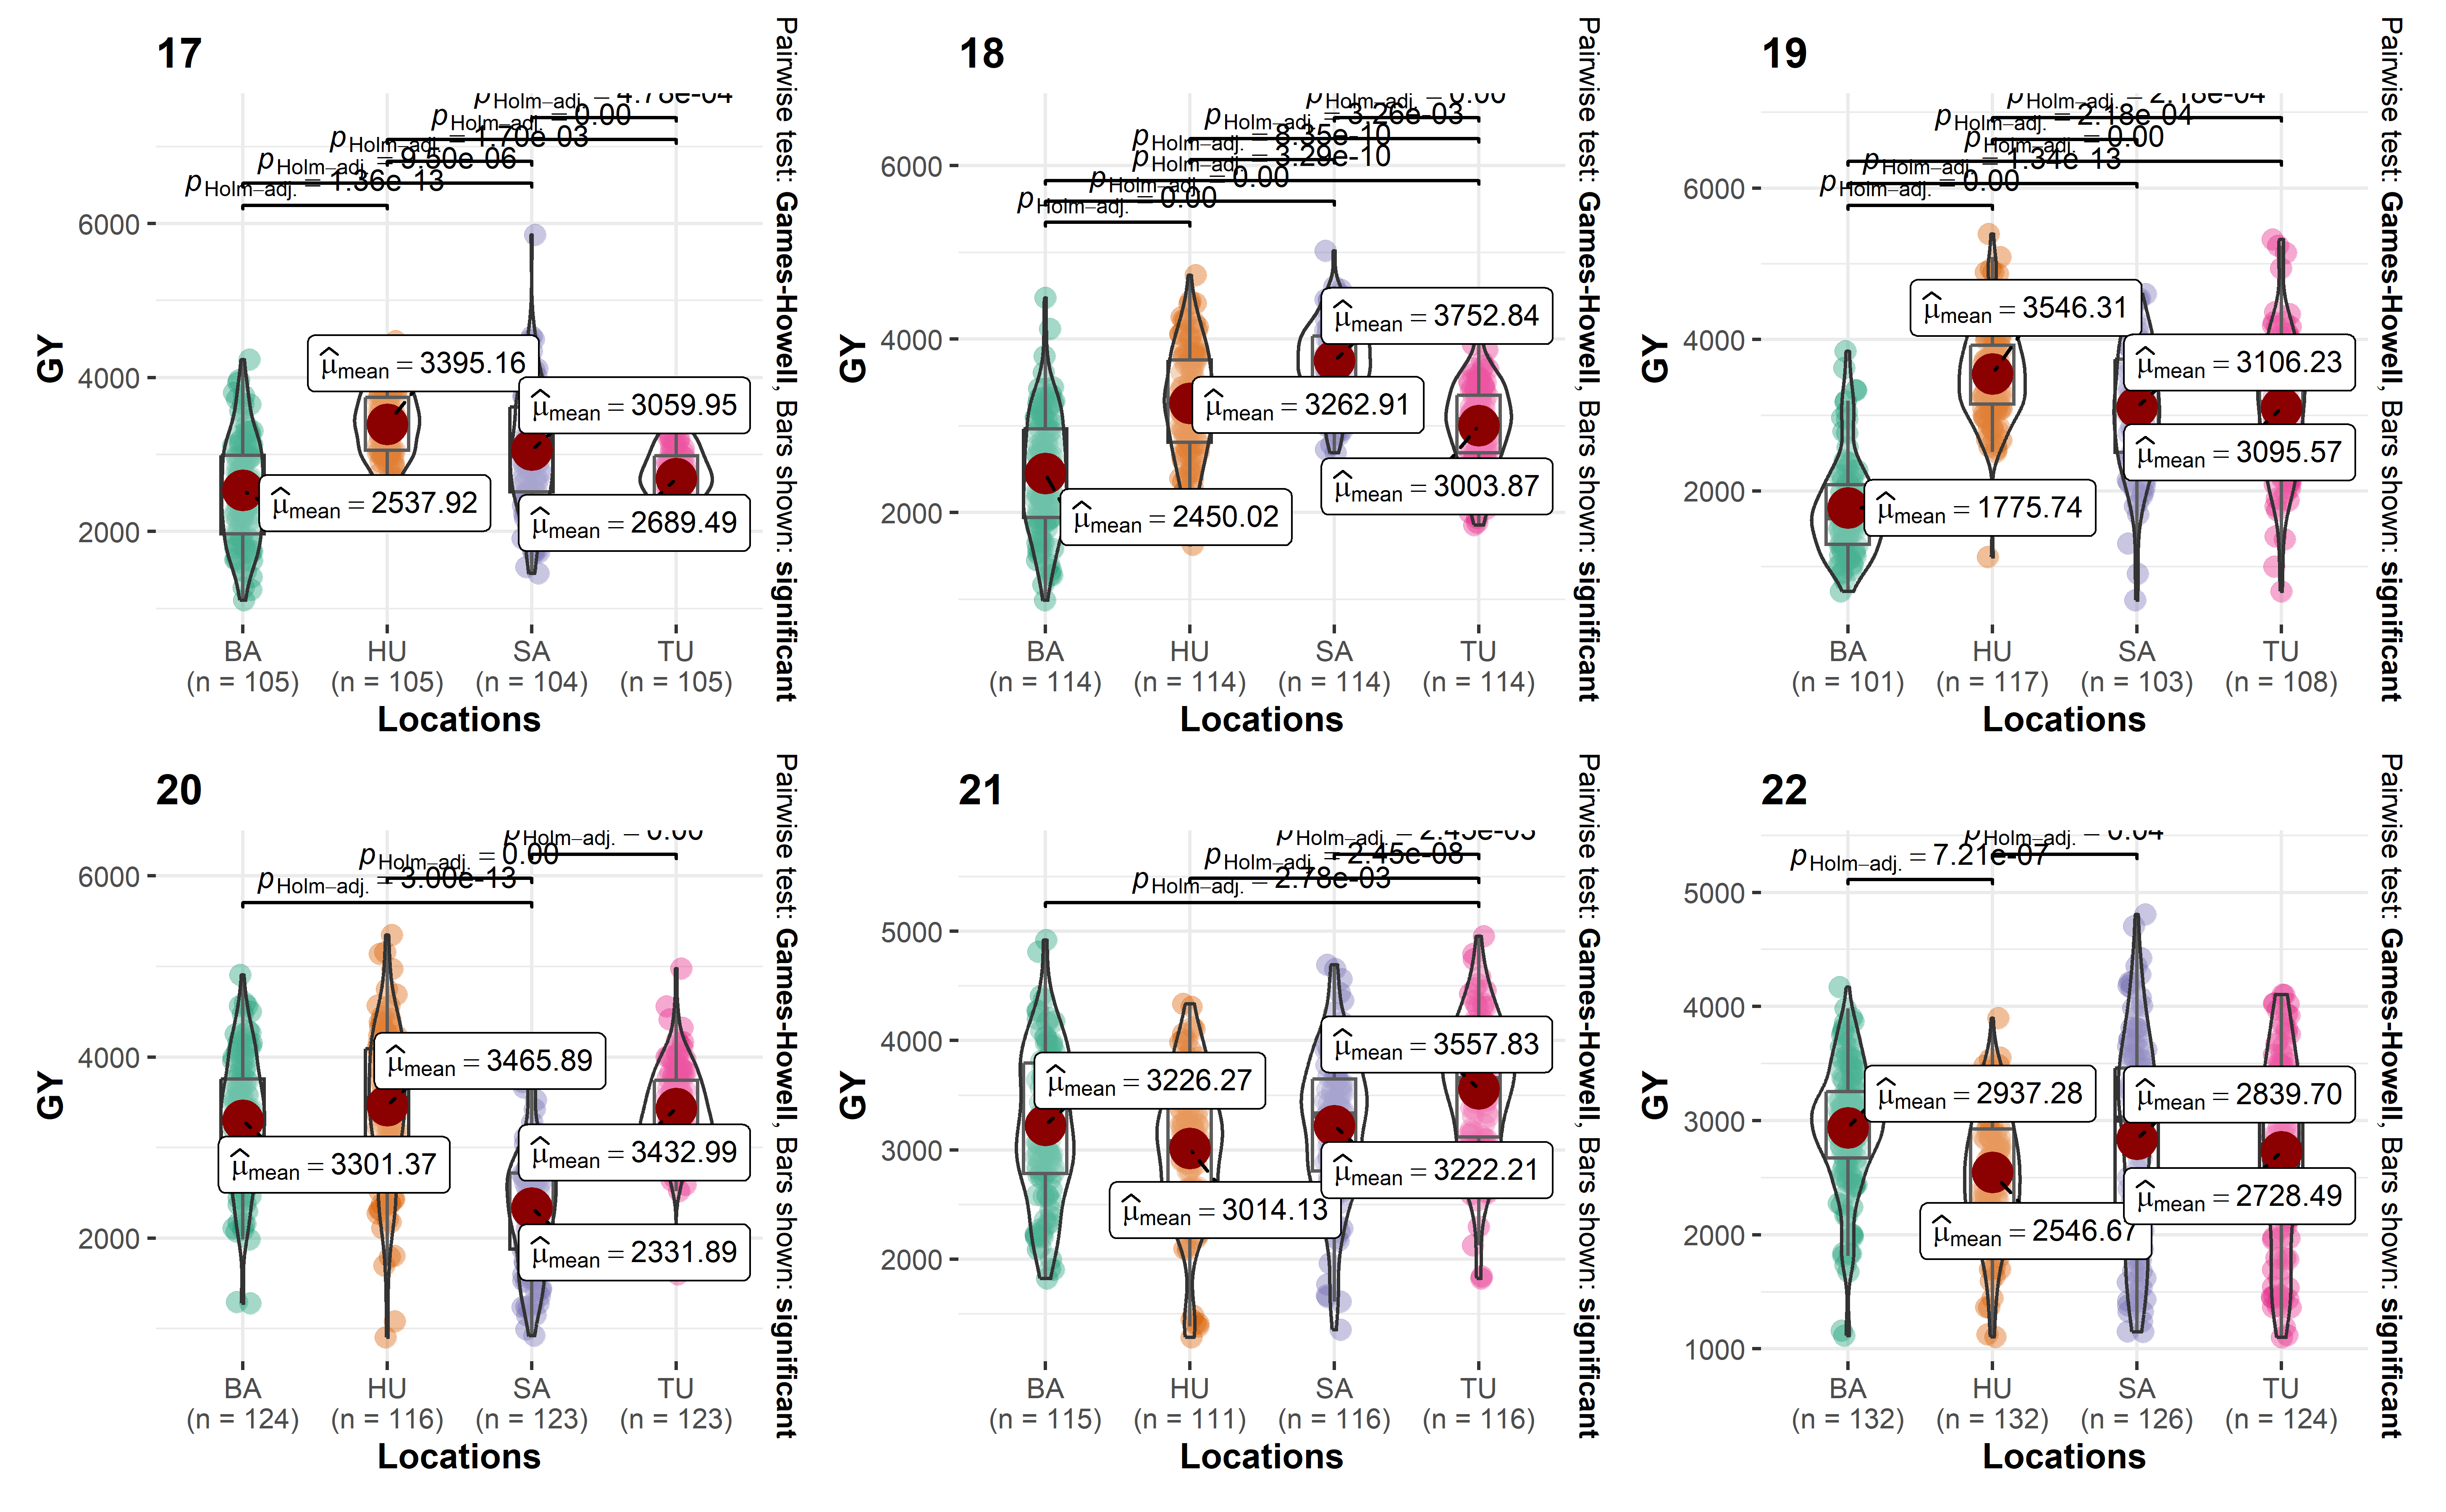
\includegraphics[width=1\linewidth]{figures/plot_ggstatsplot_desc_NB-1} \end{center}

\hypertarget{gei-comparisons-locyear---sr}{%
\subsubsection{GEI Comparisons (loc:year) -
SR}\label{gei-comparisons-locyear---sr}}

Box plots for between-subjects comparisons by locations using the R
package \texttt{ggstatsplot}. - Black beans (SR) - \textbf{Pairwise
Games-Howell test used. Comparisons showing significant values only}

\begin{Shaded}
\begin{Highlighting}[]
\NormalTok{data\_beans\_plotSR}\OtherTok{\textless{}{-}} \FunctionTok{droplevels}\NormalTok{(}\FunctionTok{subset}\NormalTok{(data\_beans, mkt}\SpecialCharTok{==}\StringTok{"SR"}\NormalTok{))}

\NormalTok{plotDM\_stats\_mkt\_loc\_SR}\OtherTok{\textless{}{-}} \FunctionTok{grouped\_ggbetweenstats}\NormalTok{(}\AttributeTok{data=}\NormalTok{data\_beans\_plotSR, }\AttributeTok{x=}\NormalTok{ loc, }\AttributeTok{y=}\NormalTok{gy\_kg\_ha, }\AttributeTok{type =} \StringTok{"parametric"}\NormalTok{,  }\AttributeTok{bf.message =}\NormalTok{ F, }\AttributeTok{results.subtitle =}\NormalTok{ F, }
                              \AttributeTok{ylab=} \StringTok{"GY"}\NormalTok{, }\AttributeTok{xlab =} \StringTok{"Locations"}\NormalTok{,}
                              \AttributeTok{plot.type =} \StringTok{"boxviolin"}\NormalTok{, }\AttributeTok{grouping.var =}\NormalTok{ year ) }
\FunctionTok{print}\NormalTok{(plotDM\_stats\_mkt\_loc\_SR)}
\end{Highlighting}
\end{Shaded}

\begin{center}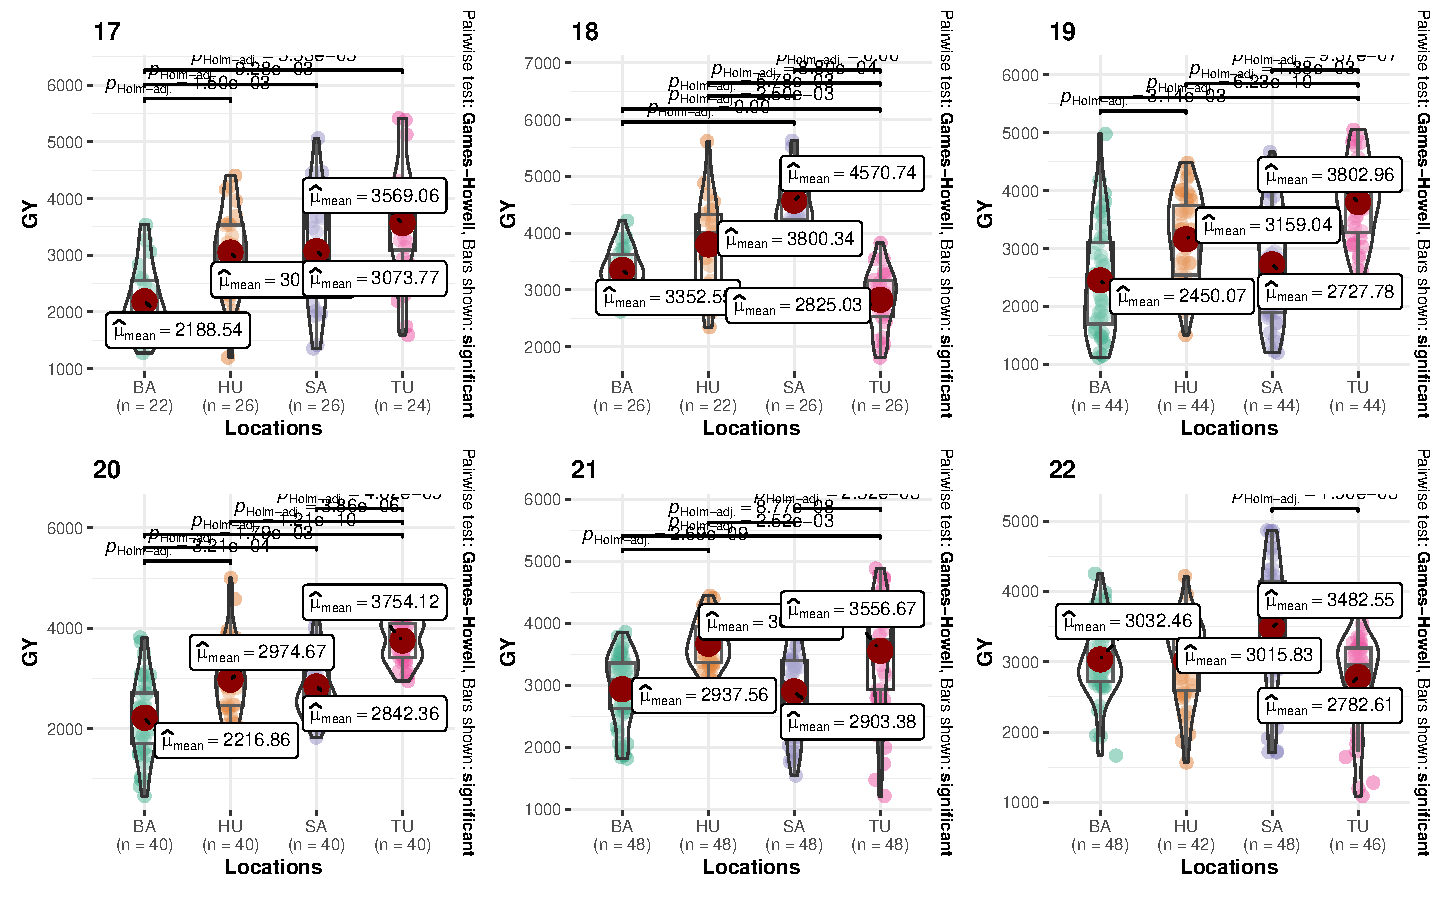
\includegraphics[width=1\linewidth]{figures/plot_ggstatsplot_desc_SR-1} \end{center}

\hypertarget{scatter-plot}{%
\subsubsection{Scatter plot}\label{scatter-plot}}

For further insight into the correlation structure between trials a
scatter plot matrix can be made using the package \texttt{statgenGxE}

\begin{Shaded}
\begin{Highlighting}[]
\NormalTok{dropsTD }\OtherTok{\textless{}{-}}\NormalTok{ statgenSTA}\SpecialCharTok{::}\FunctionTok{createTD}\NormalTok{(}\AttributeTok{data =}\NormalTok{ data\_beans, }\AttributeTok{genotype =} \StringTok{"name"}\NormalTok{, }\AttributeTok{trial =} \StringTok{"loc"}\NormalTok{)}
\FunctionTok{options}\NormalTok{(}\StringTok{"statgen.genoColors"} \OtherTok{=} \FunctionTok{c}\NormalTok{(}\StringTok{"black"}\NormalTok{, }\StringTok{"blue"}\NormalTok{, }\StringTok{"red"}\NormalTok{))}
\FunctionTok{plot}\NormalTok{(dropsTD, }\AttributeTok{plotType =} \StringTok{"scatter"}\NormalTok{, }\AttributeTok{traits =} \StringTok{"gy\_kg\_ha"}\NormalTok{, }\AttributeTok{colorGenoBy =} \StringTok{"mkt"}\NormalTok{, }
     \AttributeTok{colorTrialBy =} \StringTok{"trial"}\NormalTok{, }\AttributeTok{title =} \StringTok{"Scatterplots of trials for grain yield (Kg/ha)"}\NormalTok{ )}
\end{Highlighting}
\end{Shaded}

\begin{center}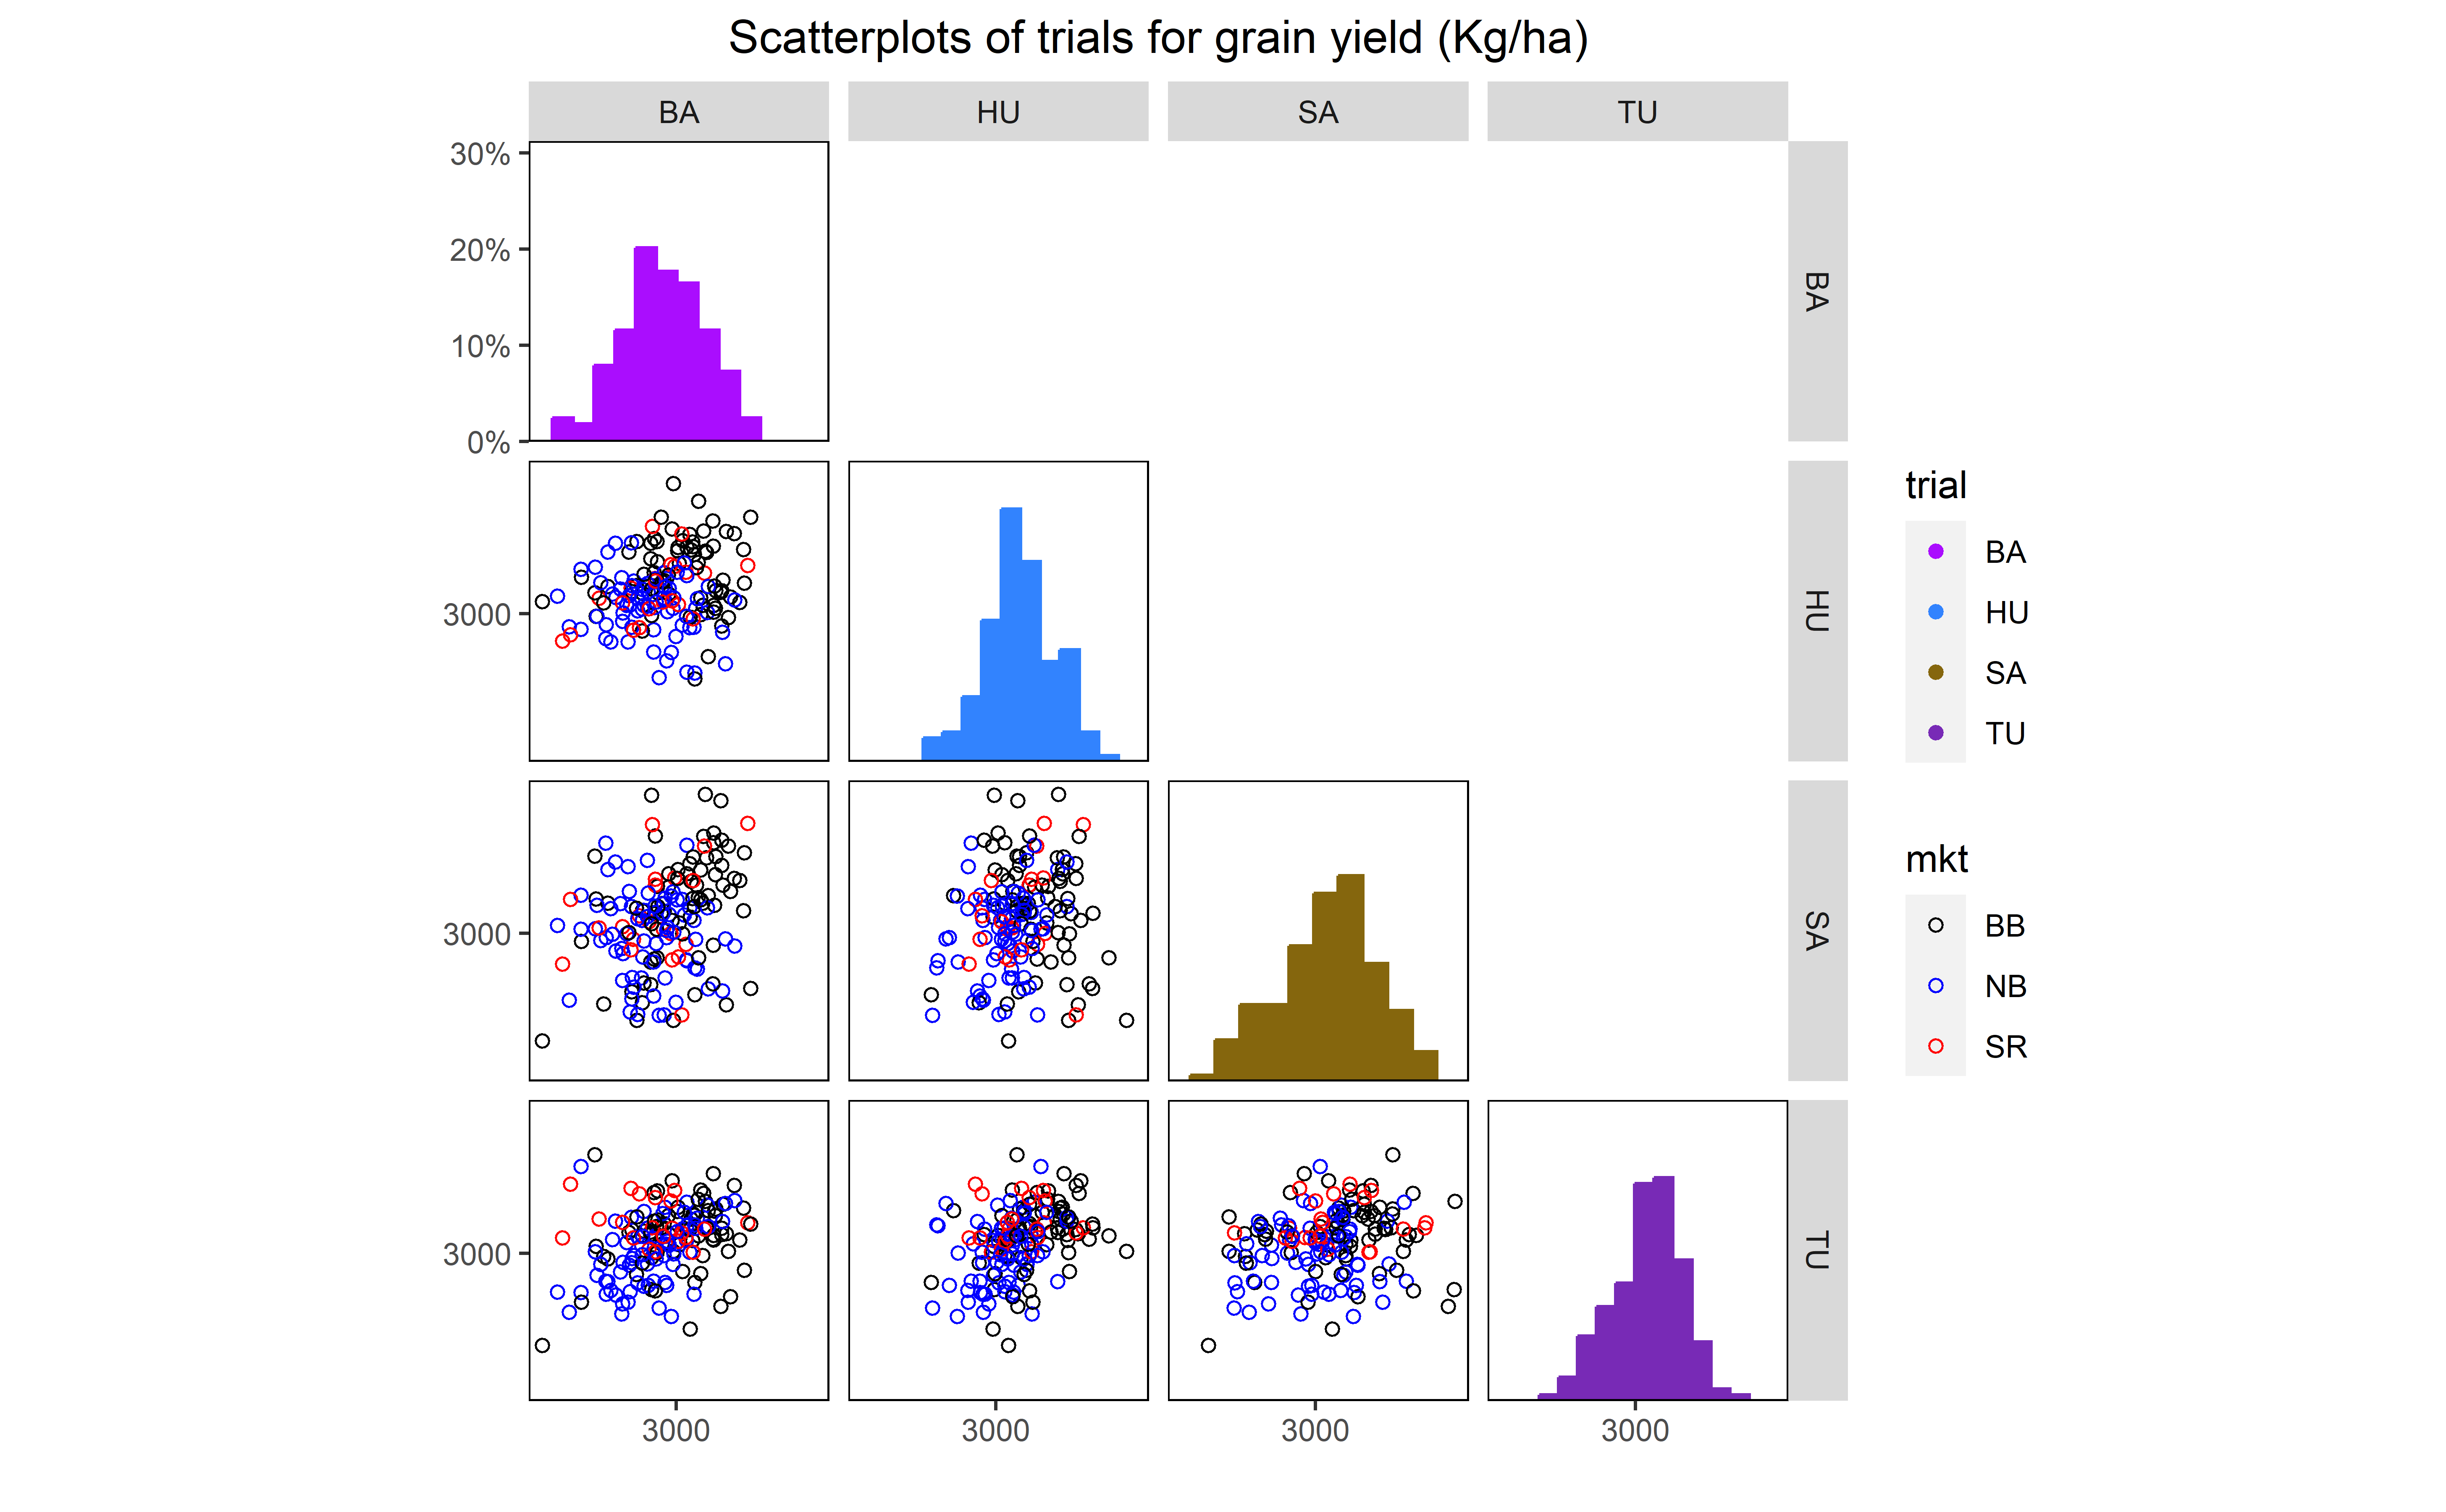
\includegraphics[width=1\linewidth]{figures/TDscatter2-1} \end{center}

\hypertarget{outliers}{%
\subsubsection{Outliers}\label{outliers}}

Check for common errors in multi-environment trial by market class data
using the R package \texttt{metan} However, the data set was cleaned
before at a previous analysis not shown in this vignette using the
criteria for GY:

\begin{itemize}
\tightlist
\item
  yield \textless= 0.5 \textbar{} yield \textgreater= 7.5 (considering
  yield as Lb per plot)
\item
  moisture \textgreater= 30 \textbar{} moisture \textless= 5
  (considering moisture in \%)
\end{itemize}

\begin{Shaded}
\begin{Highlighting}[]
\NormalTok{out\_beans}\OtherTok{\textless{}{-}} \FunctionTok{find\_outliers}\NormalTok{(data\_beans, }\AttributeTok{by=}\NormalTok{mkt, }\AttributeTok{var =}\NormalTok{ gy\_kg\_ha, }\AttributeTok{plots =}\NormalTok{ F)}
\end{Highlighting}
\end{Shaded}

Trait: gy\_kg\_ha Number of possible outliers: 9 Line(s): 1113 2052 4478
4522 4539 4620 4739 4740 4761 Proportion: 0.3\% Mean of the outliers:
3320 Maximum of the outliers: 5854 \textbar{} Line 4539 Minimum of the
outliers: 554.8 \textbar{} Line 4739 With outliers: mean = 3015
\textbar{} CV = 26.27\% Without outliers: mean = 3014 \textbar{} CV =
25.93\%

Trait: gy\_kg\_ha Number of possible outliers: 10 Line(s): 127 1910 3723
3993 4161 4358 5630 6302 6638 6710 Proportion: 0.4\% Mean of the
outliers: 4313 Maximum of the outliers: 6014 \textbar{} Line 6302
Minimum of the outliers: 889.9 \textbar{} Line 3993 With outliers: mean
= 3298 \textbar{} CV = 25.57\% Without outliers: mean = 3294 \textbar{}
CV = 25.21\%

Trait: gy\_kg\_ha Number of possible outliers: 4 Line(s): 533 1422 1951
1975 Proportion: 0.4\% Mean of the outliers: 4355 Maximum of the
outliers: 5625 \textbar{} Line 1951 Minimum of the outliers: 654.1
\textbar{} Line 533 With outliers: mean = 3139 \textbar{} CV = 27.68\%
Without outliers: mean = 3134 \textbar{} CV = 27.29\%

\begin{Shaded}
\begin{Highlighting}[]
\CommentTok{\#out\_beans}
\end{Highlighting}
\end{Shaded}

\begin{itemize}
\tightlist
\item
  No outliers removed after the data inspection based on Breeder's
  expertise.
\end{itemize}

\hypertarget{map-of-locations}{%
\subsubsection{Map of locations}\label{map-of-locations}}

\begin{Shaded}
\begin{Highlighting}[]
\FunctionTok{print}\NormalTok{(combined\_plot)}
\end{Highlighting}
\end{Shaded}

\begin{figure}[H]

{\centering 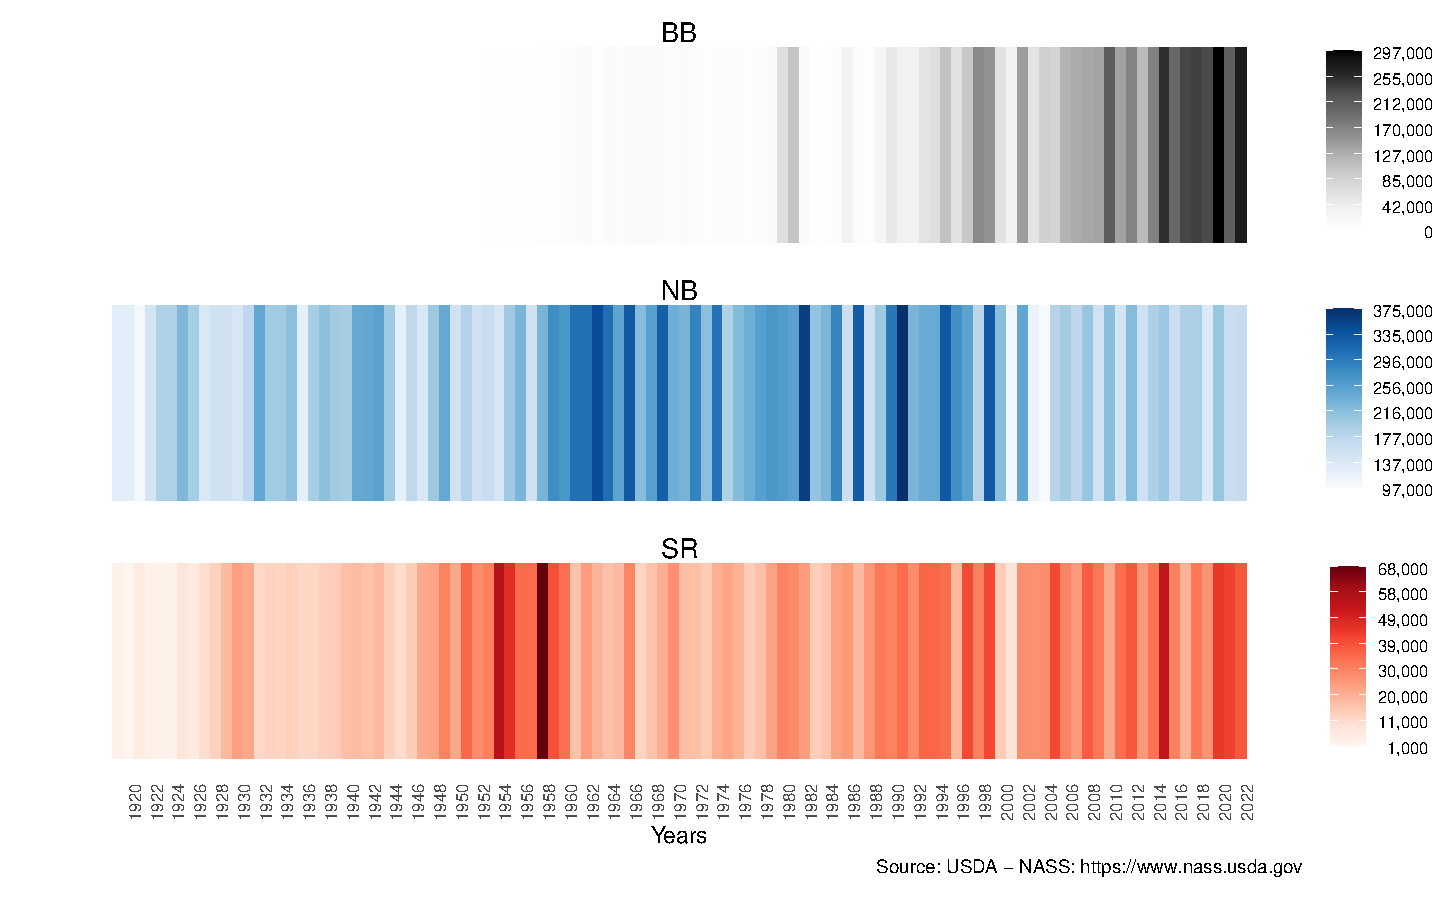
\includegraphics[width=1\linewidth]{figures/combined_plot1-1} 

}

\caption{Historical dry beans production in tons across years for black beans (BB), navy beans (NB) and small red beans (SR).}\label{fig:combined_plot1}
\end{figure}

\pagebreak

\begin{Shaded}
\begin{Highlighting}[]
\FunctionTok{print}\NormalTok{(mi\_plot)}
\end{Highlighting}
\end{Shaded}

\begin{figure}[H]

{\centering 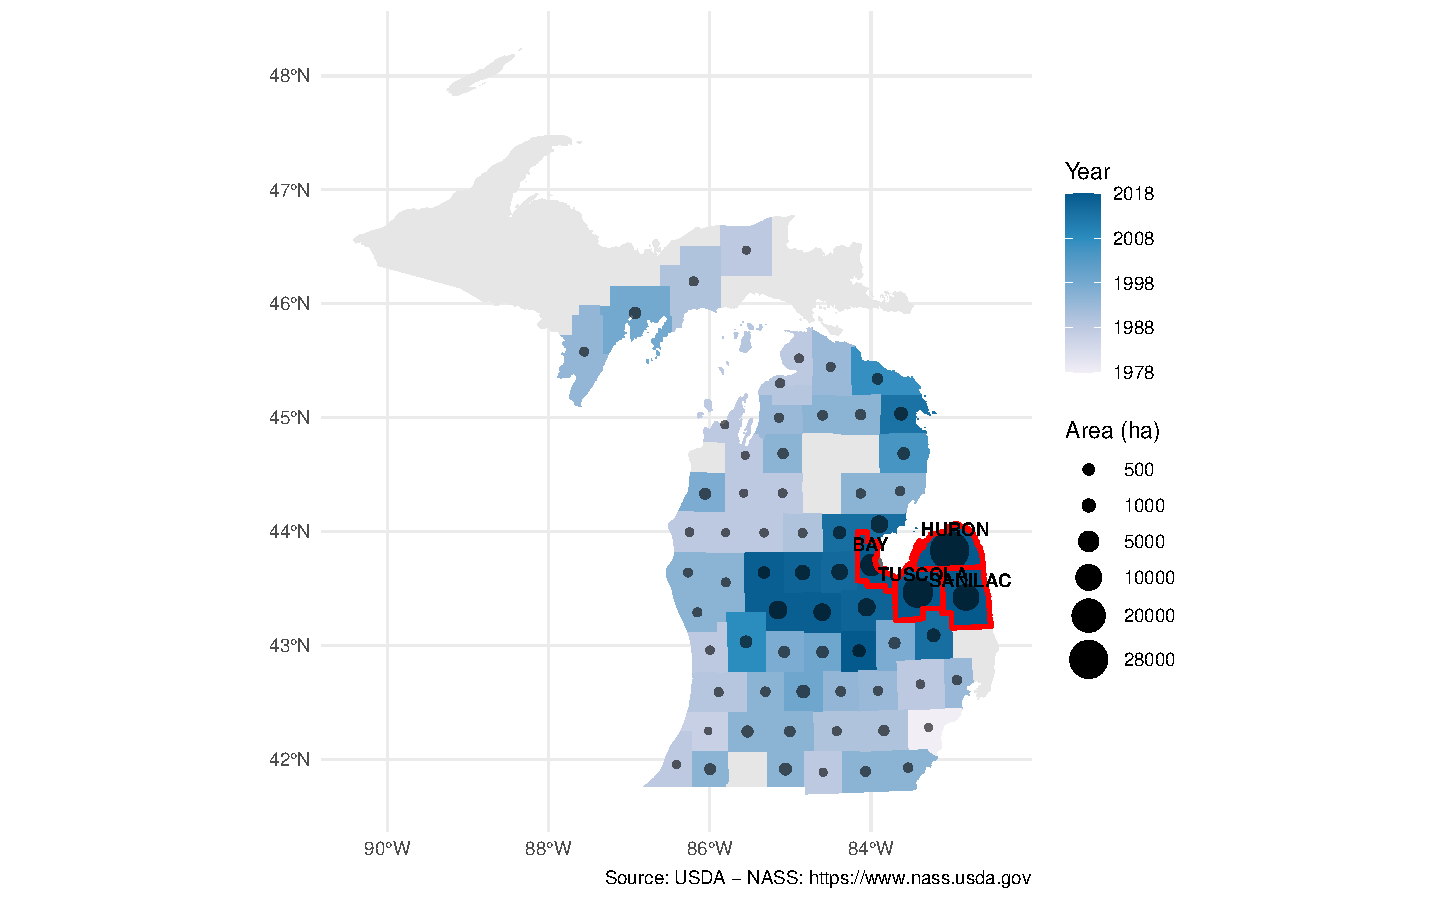
\includegraphics[width=1\linewidth]{figures/combined_plot2-1} 

}

\caption{Counties locations evaluated in this study at Michigan, mid-west in the USA. For each MI county, the blue scale shows the last year of data available.}\label{fig:combined_plot2}
\end{figure}

\pagebreak

\hypertarget{missing-values}{%
\subsubsection{Missing values}\label{missing-values}}

\begin{Shaded}
\begin{Highlighting}[]
\NormalTok{data\_beans.miss.f}\OtherTok{\textless{}{-}}\NormalTok{ data\_beans }\SpecialCharTok{\%\textgreater{}\%} 
  \FunctionTok{unite}\NormalTok{(name\_year\_loc, }\FunctionTok{c}\NormalTok{(name, year\_loc), }\AttributeTok{remove =}\NormalTok{ F) }\SpecialCharTok{\%\textgreater{}\%} 
  \FunctionTok{group\_by}\NormalTok{(name\_year\_loc) }\SpecialCharTok{\%\textgreater{}\%} 
\NormalTok{  dplyr}\SpecialCharTok{::}\FunctionTok{summarise}\NormalTok{(}\AttributeTok{Mean =} \FunctionTok{mean}\NormalTok{(gy\_kg\_ha, }\AttributeTok{na.rm =} \ConstantTok{TRUE}\NormalTok{)) }\SpecialCharTok{\%\textgreater{}\%} 
  \FunctionTok{filter}\NormalTok{(}\SpecialCharTok{!}\FunctionTok{is.na}\NormalTok{(Mean)) }

\NormalTok{data\_beans.miss}\OtherTok{\textless{}{-}}\NormalTok{ data\_beans }\SpecialCharTok{\%\textgreater{}\%} 
  \FunctionTok{unite}\NormalTok{(name\_year\_loc, }\FunctionTok{c}\NormalTok{(name, year\_loc), }\AttributeTok{remove =}\NormalTok{ F)}

\NormalTok{data\_beans.miss}\OtherTok{\textless{}{-}}\NormalTok{ data\_beans.miss}\SpecialCharTok{\%\textgreater{}\%} 
  \FunctionTok{filter}\NormalTok{((name\_year\_loc }\SpecialCharTok{\%in\%}\NormalTok{ data\_beans.miss.f}\SpecialCharTok{$}\NormalTok{name\_year\_loc))  }

\FunctionTok{gg\_miss\_fct}\NormalTok{(data\_beans.miss,}\AttributeTok{fct =}\NormalTok{ mkt)}\SpecialCharTok{+}\FunctionTok{ggtitle}\NormalTok{(}\StringTok{"Missing values (NA)"}\NormalTok{) }\SpecialCharTok{+} 
   \FunctionTok{theme}\NormalTok{(}\AttributeTok{axis.text.x=}\FunctionTok{element\_text}\NormalTok{(}\AttributeTok{face=}\StringTok{"bold"}\NormalTok{, }\AttributeTok{size =} \DecValTok{12}\NormalTok{), }
         \AttributeTok{axis.text.y =} \FunctionTok{element\_text}\NormalTok{(}\AttributeTok{face =} \StringTok{"bold"}\NormalTok{,}\AttributeTok{size =} \DecValTok{12}\NormalTok{) ,}
         \AttributeTok{title =} \FunctionTok{element\_text}\NormalTok{(}\AttributeTok{face =} \StringTok{"bold"}\NormalTok{,}\AttributeTok{size =} \DecValTok{14}\NormalTok{))}
\end{Highlighting}
\end{Shaded}

\begin{figure}[H]

{\centering 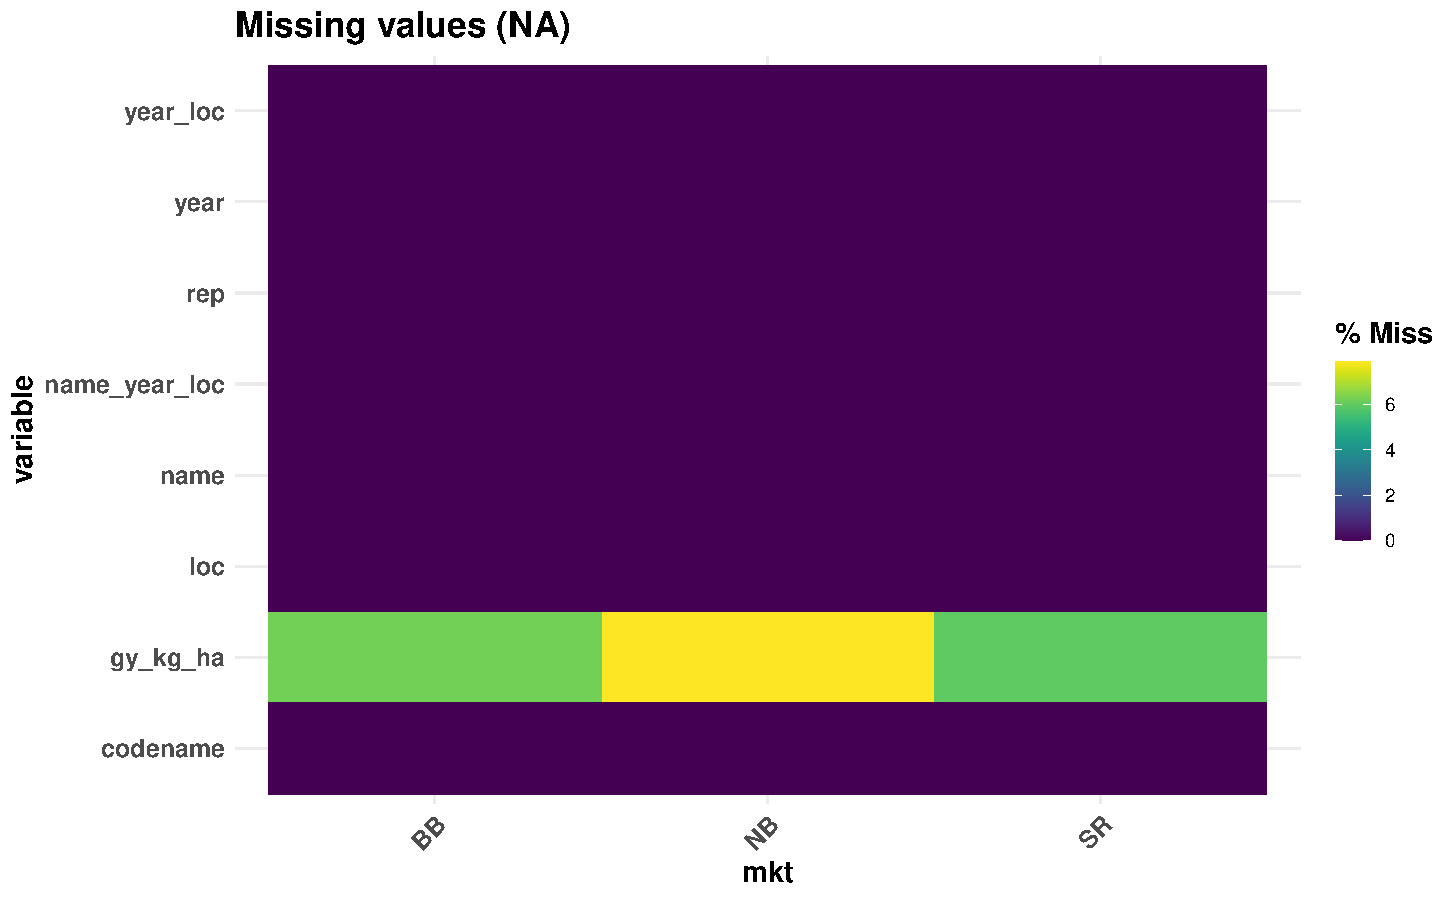
\includegraphics[width=1\linewidth]{figures/missing geno gy-1} 

}

\caption{Missing genotypes by beans market classes}\label{fig:missing geno gy}
\end{figure}

\hypertarget{coincidence-genotypes}{%
\subsubsection{Coincidence Genotypes}\label{coincidence-genotypes}}

\begin{quote}
Genotypes coincidentes across years combinations
\end{quote}

\begin{Shaded}
\begin{Highlighting}[]
\FunctionTok{source}\NormalTok{(}\StringTok{"utils/Coinc.R"}\NormalTok{)}
\end{Highlighting}
\end{Shaded}

\begin{verbatim}
#> [1] "The coincidence file is present"
\end{verbatim}

\begin{Shaded}
\begin{Highlighting}[]
\CommentTok{\#arrange\_ggplot(plotB, plotN, plotSR,ncol = 1)}

\DocumentationTok{\#\# Figure showing the results corrected across years}
\NormalTok{knitr}\SpecialCharTok{::}\FunctionTok{include\_graphics}\NormalTok{(here}\SpecialCharTok{::}\FunctionTok{here}\NormalTok{(}\StringTok{"figures"}\NormalTok{, }\StringTok{"coincidence geno fig1{-}1.png"}\NormalTok{))}
\end{Highlighting}
\end{Shaded}

\begin{figure}[H]

{\centering 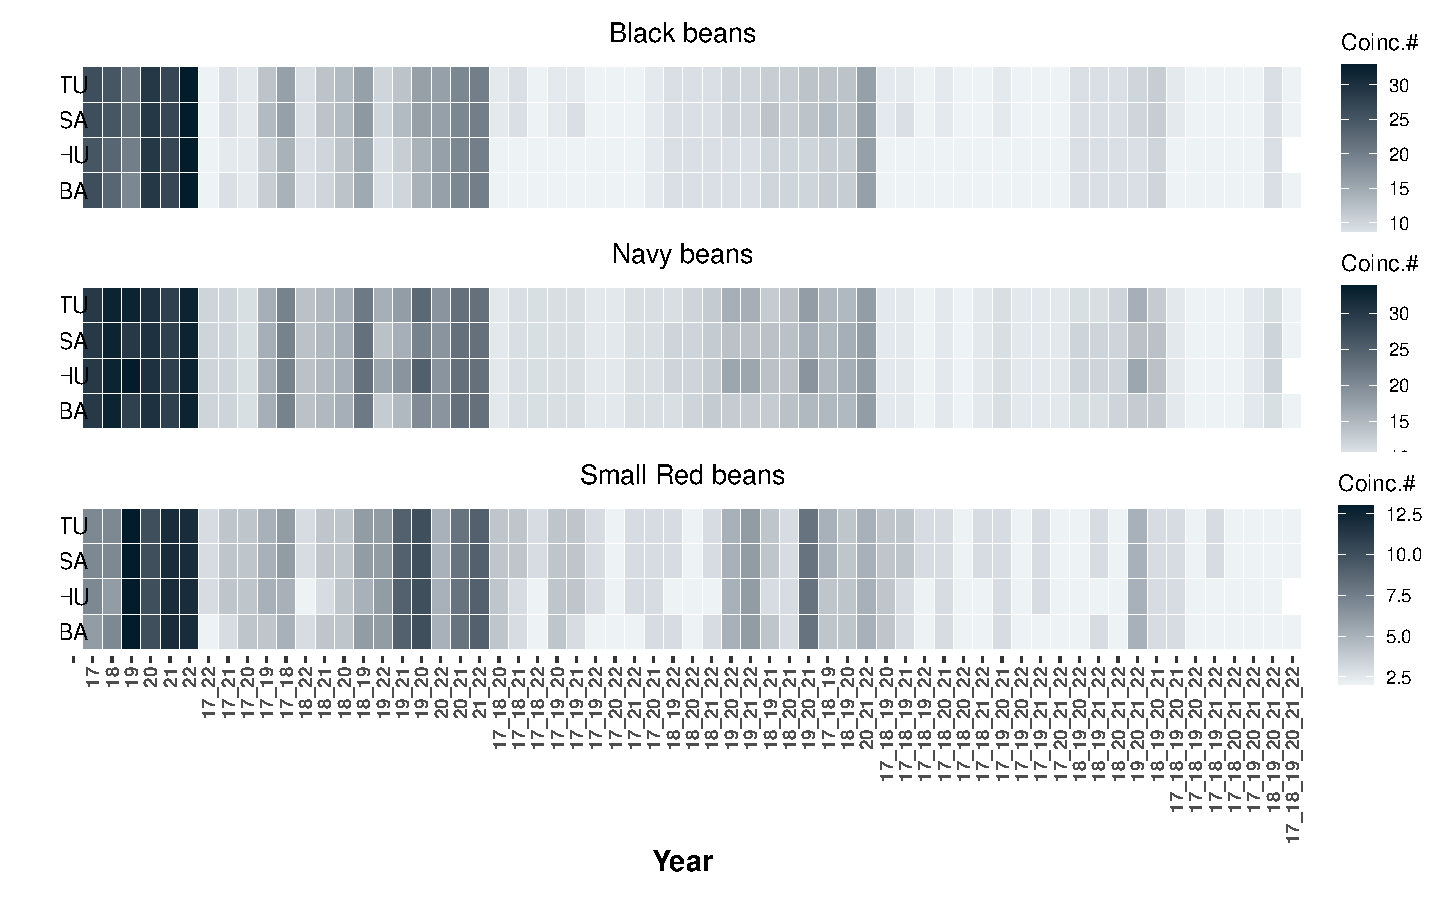
\includegraphics[width=1\linewidth]{figures/coincidence geno fig1-1} 

}

\caption{Coincidence genotypes per year and combinations of years across locations for each market class.}\label{fig:coincidence geno fig1}
\end{figure}

\hypertarget{predicted-by-year-mixed-model-analysis}{%
\subsection{Predicted by year mixed model
analysis}\label{predicted-by-year-mixed-model-analysis}}

To predict the BLUPs per year and plot it versus year: BLUPs prediction
for the vector of the variable GY in the ith genotype, and jth loc
within \texttt{year}.

\hypertarget{data-preparation-1}{%
\subsection{Data preparation}\label{data-preparation-1}}

\begin{Shaded}
\begin{Highlighting}[]
\CommentTok{\#setwd("G:/Shared drives/Bean\_Lab/Volpato/GxE\_Variety\_trials\_Scott/Manuscript/Suppl\_mat/TemplateResults{-}main")}
\NormalTok{data\_beans }\OtherTok{=} \FunctionTok{read.csv}\NormalTok{(}\StringTok{"data/DataBean\_MET\_GYv2.csv"}\NormalTok{,}\AttributeTok{h=}\NormalTok{T, }\AttributeTok{stringsAsFactors =}\NormalTok{ T)}

\CommentTok{\# Data adjustment}
\CommentTok{\# All the effect columns must be as a factor to run in ASReml{-}r.}
\NormalTok{cols }\OtherTok{\textless{}{-}} \FunctionTok{c}\NormalTok{(}\StringTok{"rep"}\NormalTok{, }\StringTok{"name"}\NormalTok{, }\StringTok{"loc"}\NormalTok{,}\StringTok{"year"}\NormalTok{, }\StringTok{"mkt"}\NormalTok{, }\StringTok{"year\_loc"}\NormalTok{)}
\NormalTok{data\_beans[cols] }\OtherTok{\textless{}{-}} \FunctionTok{lapply}\NormalTok{(data\_beans[cols], factor)}
\NormalTok{data\_beans }\OtherTok{\textless{}{-}} \FunctionTok{data.table}\NormalTok{(data\_beans)}
\end{Highlighting}
\end{Shaded}

\hypertarget{by-year-mixed-model-analysis}{%
\subsubsection{By year mixed model
analysis}\label{by-year-mixed-model-analysis}}

The BLUPS will be estimated using a mixed-effect model and these values
obtained by year using a loop with \texttt{ASReml} and storage into the
list.

The following mixed model was used to estimate the BLUPs of each
genotype within year with one value per genotype per year (random
effects are underlined in all equations):

\[
\underline{Y_{ijl}} = \mu  + \underline{G_i} + {E_{l}} + \beta_{jl} + \underline{GE_{il}} + \underline{\varepsilon_{ijl}} 
\]

where \({Y_{ijl}}\) is the response variable (e.g., grain yield)
observed in the \emph{j}th repetion of the \emph{i}th genotype in the
\emph{l}th location (\emph{i} = 1, 2, \ldots, \emph{g}; \emph{j} = 1, 2,
\ldots, \emph{b}; \emph{l} = 1, 2, \ldots, \emph{e}); \(\mu\) is the
grand mean; \(\underline{G_i}\) is the effect of the \emph{i}th
genotype; \(E_l\) is the effect of the \emph{l}th location (env);
\(\beta_{jl}\) is the effect of the \emph{j}th rep with the \emph{l}th
location; \(\underline{GE_{il}}\) is the interaction effect of the
\emph{i}th genotype nested within the \emph{l}th location; and
\(\mathop \varepsilon \nolimits_{ijl}\) is the random error, in witch
with \(G_{i}\)\textasciitilde N(0,\(\sigma_{G}^{2}\)),
\(GE_{il}\)\textasciitilde N(0,\(\sigma_{GE}^{2}\)), and
\(\varepsilon_{ijl}\)\textasciitilde N(0,\(\sigma_{\varepsilon}^{2}\)),
all independent, where \(G_{G}^{2}\) is the genotype (name)
variance,\(GS_{GE}^{2}\) is the interaction genotype x environment
variance, and \(\sigma_{\varepsilon}^{2}\) is the mean error variance
across experiments.

\begin{Shaded}
\begin{Highlighting}[]
\DocumentationTok{\#\# Analysis per site and mkt class}
\NormalTok{mkt\_n }\OtherTok{\textless{}{-}} \FunctionTok{levels}\NormalTok{(data\_beans}\SpecialCharTok{$}\NormalTok{mkt)}

\NormalTok{Envs }\OtherTok{\textless{}{-}} \FunctionTok{levels}\NormalTok{(data\_beans}\SpecialCharTok{$}\NormalTok{year)}

\NormalTok{stgI\_list }\OtherTok{\textless{}{-}} \FunctionTok{matrix}\NormalTok{(}\AttributeTok{data=}\FunctionTok{list}\NormalTok{(), }\AttributeTok{nrow=}\FunctionTok{length}\NormalTok{(Envs), }\AttributeTok{ncol=}\DecValTok{1}\NormalTok{,}
                    \AttributeTok{dimnames=}\FunctionTok{list}\NormalTok{(Envs, }\FunctionTok{c}\NormalTok{(}\StringTok{"BLUPS"}\NormalTok{)))}

\NormalTok{mkt }\OtherTok{\textless{}{-}} \FunctionTok{nlevels}\NormalTok{(data\_beans}\SpecialCharTok{$}\NormalTok{mkt)}

\ControlFlowTok{for}\NormalTok{(k }\ControlFlowTok{in} \DecValTok{1}\SpecialCharTok{:}\NormalTok{mkt)\{}

\NormalTok{  bk }\OtherTok{\textless{}{-}} \FunctionTok{levels}\NormalTok{(data\_beans}\SpecialCharTok{$}\NormalTok{mkt)}
\NormalTok{  cj }\OtherTok{\textless{}{-}}\NormalTok{ bk[k]}
  \CommentTok{\#print(cj)}
  
\NormalTok{  data\_beans\_temp }\OtherTok{\textless{}{-}} \FunctionTok{droplevels}\NormalTok{(}\FunctionTok{subset}\NormalTok{(data\_beans, mkt}\SpecialCharTok{==}\NormalTok{cj))}

  \ControlFlowTok{for}\NormalTok{ (i }\ControlFlowTok{in}\NormalTok{ Envs)\{}
    \CommentTok{\#i=Envs[1]}
\NormalTok{    Edat }\OtherTok{\textless{}{-}} \FunctionTok{droplevels}\NormalTok{(}\FunctionTok{subset}\NormalTok{(data\_beans\_temp, year}\SpecialCharTok{==}\NormalTok{i))}
    
    \CommentTok{\#print(i)}
    
\NormalTok{mod}\FloatTok{.1} \OtherTok{\textless{}{-}} \FunctionTok{asreml}\NormalTok{(}\AttributeTok{fixed       =}\NormalTok{ gy\_kg\_ha }\SpecialCharTok{\textasciitilde{}}\NormalTok{  loc }\SpecialCharTok{+}\NormalTok{ loc}\SpecialCharTok{:}\NormalTok{rep,}
                     \AttributeTok{random      =} \SpecialCharTok{\textasciitilde{}}\NormalTok{  name }\SpecialCharTok{+}\NormalTok{ name}\SpecialCharTok{:}\NormalTok{loc,}
                     \AttributeTok{data        =}\NormalTok{ Edat,}
                     \AttributeTok{predict     =} \FunctionTok{predict.asreml}\NormalTok{(}\AttributeTok{classify =} \StringTok{"name"}\NormalTok{),}
                     \AttributeTok{trace       =}\NormalTok{ F,}
                     \AttributeTok{maxit       =} \DecValTok{500}\NormalTok{)}
    
   \CommentTok{\# print(summary.asreml(mod.1)$varcomp)}
    \CommentTok{\# wald(mod.1)}

\NormalTok{  blup}\FloatTok{.1}\OtherTok{\textless{}{-}} \FunctionTok{as.data.frame}\NormalTok{((mod}\FloatTok{.1}\SpecialCharTok{$}\NormalTok{predictions}\SpecialCharTok{$}\NormalTok{pvals[}\DecValTok{1}\SpecialCharTok{:}\DecValTok{3}\NormalTok{])) }
  \FunctionTok{names}\NormalTok{(blup}\FloatTok{.1}\NormalTok{) }\OtherTok{\textless{}{-}} \FunctionTok{c}\NormalTok{(}\StringTok{"name"}\NormalTok{, }\StringTok{"yield"}\NormalTok{, }\StringTok{"se"}\NormalTok{)}
\NormalTok{  blup}\FloatTok{.1}\SpecialCharTok{$}\NormalTok{mkt}\OtherTok{\textless{}{-}}\NormalTok{ cj}
  
\NormalTok{    stgI\_list[[i, }\StringTok{"BLUPS"}\NormalTok{]] }\OtherTok{\textless{}{-}}\NormalTok{ blup}\FloatTok{.1} \CommentTok{\# put all the results of Stage 1 in the list}
    
   \CommentTok{\# rm(Edat,mod.1, blue, blup.1)}
    
\NormalTok{  \}}
   \ControlFlowTok{if}\NormalTok{(k}\SpecialCharTok{==}\DecValTok{1}\NormalTok{)\{stgI\_list}\FloatTok{.1}\OtherTok{\textless{}{-}}\NormalTok{stgI\_list\}}\ControlFlowTok{else}\NormalTok{\{stgI\_list}\FloatTok{.1}\OtherTok{\textless{}{-}}\FunctionTok{rbind}\NormalTok{(stgI\_list}\FloatTok{.1}\NormalTok{, stgI\_list)\}}
   
\NormalTok{\}}
\end{Highlighting}
\end{Shaded}

\hypertarget{preparing-dataset}{%
\paragraph{Preparing dataset}\label{preparing-dataset}}

Merging the original data to have all the factors in the final table
with: \texttt{name}, \texttt{year}, and \texttt{mkt}

\begin{Shaded}
\begin{Highlighting}[]
\DocumentationTok{\#\#\#\#\# Unlist the results of Stage I and format as data.table \#\#\#\#\#}
\NormalTok{blups\_stageI }\OtherTok{\textless{}{-}} \FunctionTok{data.table}\NormalTok{(}\FunctionTok{ldply}\NormalTok{(stgI\_list}\FloatTok{.1}\NormalTok{[, }\StringTok{"BLUPS"}\NormalTok{], data.frame, }\AttributeTok{.id=}\StringTok{"year"}\NormalTok{))}

\NormalTok{blues\_stage.I }\OtherTok{\textless{}{-}}\NormalTok{ blups\_stageI[}\FunctionTok{order}\NormalTok{(blups\_stageI}\SpecialCharTok{$}\NormalTok{year,blups\_stageI}\SpecialCharTok{$}\NormalTok{mkt),]}

\CommentTok{\# Change the order of columns}
\NormalTok{blues\_stage.I }\OtherTok{\textless{}{-}}\NormalTok{ blues\_stage.I }\SpecialCharTok{\%\textgreater{}\%} 
\NormalTok{  dplyr}\SpecialCharTok{::}\FunctionTok{select}\NormalTok{(year, name, mkt, se, yield)}

\FunctionTok{str}\NormalTok{(blues\_stage.I)}
\end{Highlighting}
\end{Shaded}

Classes `data.table' and `data.frame': 984 obs. of 5 variables: \$ year
: Factor w/ 6 levels ``17'',``18'',``19'',..: 1 1 1 1 1 1 1 1 1 1
\ldots{} \$ name : chr ``B1'' ``B10'' ``B11'' ``B12'' \ldots{} \$ mkt :
chr ``BB'' ``BB'' ``BB'' ``BB'' \ldots{} \$ se : num 141.3 98.7 113.8
113.8 355.7 \ldots{} \$ yield: num 2727 3579 2947 3092 2959 \ldots{} -
attr(*, ``.internal.selfref'')=

\hypertarget{descriptive-variance}{%
\subsubsection{Descriptive variance}\label{descriptive-variance}}

\hypertarget{beans-data-set-by-year}{%
\paragraph{Beans data set by year}\label{beans-data-set-by-year}}

\begin{Shaded}
\begin{Highlighting}[]
\ControlFlowTok{if}\NormalTok{ (knitr}\SpecialCharTok{::}\FunctionTok{is\_html\_output}\NormalTok{()) \{}

  \FunctionTok{print\_table}\NormalTok{(blues\_stage.I)}
  
\NormalTok{\}}\ControlFlowTok{else}\NormalTok{\{}
 
\FunctionTok{flextable}\NormalTok{(}\FunctionTok{head}\NormalTok{(blues\_stage.I)) }\SpecialCharTok{\%\textgreater{}\%} 
   \FunctionTok{add\_footer\_lines}\NormalTok{(}
     \FunctionTok{c}\NormalTok{(}\StringTok{"Beans data set by year"}\NormalTok{, }
       \StringTok{"Header data set showing the 6 first entry"}\NormalTok{)) }\SpecialCharTok{\%\textgreater{}\%} 
   \FunctionTok{autofit}\NormalTok{() }\SpecialCharTok{\%\textgreater{}\%} 
   \FunctionTok{add\_header\_lines}\NormalTok{(}\StringTok{"Dry Beans varieties trial"}\NormalTok{) }\SpecialCharTok{\%\textgreater{}\%} 
  \FunctionTok{theme\_design2}\NormalTok{()}
  
\NormalTok{\}}
\end{Highlighting}
\end{Shaded}

\global\setlength{\Oldarrayrulewidth}{\arrayrulewidth}

\global\setlength{\Oldtabcolsep}{\tabcolsep}

\setlength{\tabcolsep}{0pt}

\renewcommand*{\arraystretch}{1.5}



\providecommand{\ascline}[3]{\noalign{\global\arrayrulewidth #1}\arrayrulecolor[HTML]{#2}\cline{#3}}

\begin{longtable}[c]{|p{0.75in}|p{0.75in}|p{0.75in}|p{0.75in}|p{0.75in}}



\ascline{1.5pt}{666666}{1-5}

\multicolumn{5}{>{\raggedright}m{\dimexpr 3.75in+8\tabcolsep}}{\textcolor[HTML]{000000}{\fontsize{10}{10}\selectfont{\global\setmainfont{Arial}{\textbf{Dry\ Beans\ varieties\ trial}}}}} \\

\ascline{0.75pt}{666666}{1-5}



\multicolumn{1}{>{\raggedright}m{\dimexpr 0.75in+0\tabcolsep}}{\textcolor[HTML]{000000}{\fontsize{10}{10}\selectfont{\global\setmainfont{Arial}{\textbf{year}}}}} & \multicolumn{1}{>{\raggedright}m{\dimexpr 0.75in+0\tabcolsep}}{\textcolor[HTML]{000000}{\fontsize{10}{10}\selectfont{\global\setmainfont{Arial}{\textbf{name}}}}} & \multicolumn{1}{>{\raggedright}m{\dimexpr 0.75in+0\tabcolsep}}{\textcolor[HTML]{000000}{\fontsize{10}{10}\selectfont{\global\setmainfont{Arial}{\textbf{mkt}}}}} & \multicolumn{1}{>{\raggedleft}m{\dimexpr 0.75in+0\tabcolsep}}{\textcolor[HTML]{000000}{\fontsize{10}{10}\selectfont{\global\setmainfont{Arial}{\textbf{se}}}}} & \multicolumn{1}{>{\raggedleft}m{\dimexpr 0.75in+0\tabcolsep}}{\textcolor[HTML]{000000}{\fontsize{10}{10}\selectfont{\global\setmainfont{Arial}{\textbf{yield}}}}} \\

\ascline{1.5pt}{666666}{1-5}\endfirsthead

\ascline{1.5pt}{666666}{1-5}

\multicolumn{5}{>{\raggedright}m{\dimexpr 3.75in+8\tabcolsep}}{\textcolor[HTML]{000000}{\fontsize{10}{10}\selectfont{\global\setmainfont{Arial}{\textbf{Dry\ Beans\ varieties\ trial}}}}} \\

\ascline{0.75pt}{666666}{1-5}



\multicolumn{1}{>{\raggedright}m{\dimexpr 0.75in+0\tabcolsep}}{\textcolor[HTML]{000000}{\fontsize{10}{10}\selectfont{\global\setmainfont{Arial}{\textbf{year}}}}} & \multicolumn{1}{>{\raggedright}m{\dimexpr 0.75in+0\tabcolsep}}{\textcolor[HTML]{000000}{\fontsize{10}{10}\selectfont{\global\setmainfont{Arial}{\textbf{name}}}}} & \multicolumn{1}{>{\raggedright}m{\dimexpr 0.75in+0\tabcolsep}}{\textcolor[HTML]{000000}{\fontsize{10}{10}\selectfont{\global\setmainfont{Arial}{\textbf{mkt}}}}} & \multicolumn{1}{>{\raggedleft}m{\dimexpr 0.75in+0\tabcolsep}}{\textcolor[HTML]{000000}{\fontsize{10}{10}\selectfont{\global\setmainfont{Arial}{\textbf{se}}}}} & \multicolumn{1}{>{\raggedleft}m{\dimexpr 0.75in+0\tabcolsep}}{\textcolor[HTML]{000000}{\fontsize{10}{10}\selectfont{\global\setmainfont{Arial}{\textbf{yield}}}}} \\

\ascline{1.5pt}{666666}{1-5}\endhead



\multicolumn{5}{>{\raggedright}m{\dimexpr 3.75in+8\tabcolsep}}{\textcolor[HTML]{000000}{\fontsize{8}{8}\selectfont{\global\setmainfont{Arial}{Beans\ data\ set\ by\ year}}}} \\

\ascline{0.75pt}{666666}{1-5}



\multicolumn{5}{>{\raggedright}m{\dimexpr 3.75in+8\tabcolsep}}{\textcolor[HTML]{000000}{\fontsize{8}{8}\selectfont{\global\setmainfont{Arial}{Header\ data\ set\ showing\ the\ 6\ first\ entry}}}} \\

\ascline{0.75pt}{666666}{1-5}\endfoot



\multicolumn{1}{>{\raggedright}m{\dimexpr 0.75in+0\tabcolsep}}{\textcolor[HTML]{000000}{\fontsize{9}{9}\selectfont{\global\setmainfont{Arial}{17}}}} & \multicolumn{1}{>{\raggedright}m{\dimexpr 0.75in+0\tabcolsep}}{\textcolor[HTML]{000000}{\fontsize{9}{9}\selectfont{\global\setmainfont{Arial}{B1}}}} & \multicolumn{1}{>{\raggedright}m{\dimexpr 0.75in+0\tabcolsep}}{\textcolor[HTML]{000000}{\fontsize{9}{9}\selectfont{\global\setmainfont{Arial}{BB}}}} & \multicolumn{1}{>{\raggedleft}m{\dimexpr 0.75in+0\tabcolsep}}{\textcolor[HTML]{000000}{\fontsize{9}{9}\selectfont{\global\setmainfont{Arial}{141.29}}}} & \multicolumn{1}{>{\raggedleft}m{\dimexpr 0.75in+0\tabcolsep}}{\textcolor[HTML]{000000}{\fontsize{9}{9}\selectfont{\global\setmainfont{Arial}{2,727}}}} \\

\ascline{0.75pt}{666666}{1-5}



\multicolumn{1}{>{\raggedright}m{\dimexpr 0.75in+0\tabcolsep}}{\textcolor[HTML]{000000}{\fontsize{9}{9}\selectfont{\global\setmainfont{Arial}{17}}}} & \multicolumn{1}{>{\raggedright}m{\dimexpr 0.75in+0\tabcolsep}}{\textcolor[HTML]{000000}{\fontsize{9}{9}\selectfont{\global\setmainfont{Arial}{B10}}}} & \multicolumn{1}{>{\raggedright}m{\dimexpr 0.75in+0\tabcolsep}}{\textcolor[HTML]{000000}{\fontsize{9}{9}\selectfont{\global\setmainfont{Arial}{BB}}}} & \multicolumn{1}{>{\raggedleft}m{\dimexpr 0.75in+0\tabcolsep}}{\textcolor[HTML]{000000}{\fontsize{9}{9}\selectfont{\global\setmainfont{Arial}{98.73}}}} & \multicolumn{1}{>{\raggedleft}m{\dimexpr 0.75in+0\tabcolsep}}{\textcolor[HTML]{000000}{\fontsize{9}{9}\selectfont{\global\setmainfont{Arial}{3,579}}}} \\

\ascline{0.75pt}{666666}{1-5}



\multicolumn{1}{>{\raggedright}m{\dimexpr 0.75in+0\tabcolsep}}{\textcolor[HTML]{000000}{\fontsize{9}{9}\selectfont{\global\setmainfont{Arial}{17}}}} & \multicolumn{1}{>{\raggedright}m{\dimexpr 0.75in+0\tabcolsep}}{\textcolor[HTML]{000000}{\fontsize{9}{9}\selectfont{\global\setmainfont{Arial}{B11}}}} & \multicolumn{1}{>{\raggedright}m{\dimexpr 0.75in+0\tabcolsep}}{\textcolor[HTML]{000000}{\fontsize{9}{9}\selectfont{\global\setmainfont{Arial}{BB}}}} & \multicolumn{1}{>{\raggedleft}m{\dimexpr 0.75in+0\tabcolsep}}{\textcolor[HTML]{000000}{\fontsize{9}{9}\selectfont{\global\setmainfont{Arial}{113.83}}}} & \multicolumn{1}{>{\raggedleft}m{\dimexpr 0.75in+0\tabcolsep}}{\textcolor[HTML]{000000}{\fontsize{9}{9}\selectfont{\global\setmainfont{Arial}{2,947}}}} \\

\ascline{0.75pt}{666666}{1-5}



\multicolumn{1}{>{\raggedright}m{\dimexpr 0.75in+0\tabcolsep}}{\textcolor[HTML]{000000}{\fontsize{9}{9}\selectfont{\global\setmainfont{Arial}{17}}}} & \multicolumn{1}{>{\raggedright}m{\dimexpr 0.75in+0\tabcolsep}}{\textcolor[HTML]{000000}{\fontsize{9}{9}\selectfont{\global\setmainfont{Arial}{B12}}}} & \multicolumn{1}{>{\raggedright}m{\dimexpr 0.75in+0\tabcolsep}}{\textcolor[HTML]{000000}{\fontsize{9}{9}\selectfont{\global\setmainfont{Arial}{BB}}}} & \multicolumn{1}{>{\raggedleft}m{\dimexpr 0.75in+0\tabcolsep}}{\textcolor[HTML]{000000}{\fontsize{9}{9}\selectfont{\global\setmainfont{Arial}{113.83}}}} & \multicolumn{1}{>{\raggedleft}m{\dimexpr 0.75in+0\tabcolsep}}{\textcolor[HTML]{000000}{\fontsize{9}{9}\selectfont{\global\setmainfont{Arial}{3,092}}}} \\

\ascline{0.75pt}{666666}{1-5}



\multicolumn{1}{>{\raggedright}m{\dimexpr 0.75in+0\tabcolsep}}{\textcolor[HTML]{000000}{\fontsize{9}{9}\selectfont{\global\setmainfont{Arial}{17}}}} & \multicolumn{1}{>{\raggedright}m{\dimexpr 0.75in+0\tabcolsep}}{\textcolor[HTML]{000000}{\fontsize{9}{9}\selectfont{\global\setmainfont{Arial}{B13}}}} & \multicolumn{1}{>{\raggedright}m{\dimexpr 0.75in+0\tabcolsep}}{\textcolor[HTML]{000000}{\fontsize{9}{9}\selectfont{\global\setmainfont{Arial}{BB}}}} & \multicolumn{1}{>{\raggedleft}m{\dimexpr 0.75in+0\tabcolsep}}{\textcolor[HTML]{000000}{\fontsize{9}{9}\selectfont{\global\setmainfont{Arial}{355.72}}}} & \multicolumn{1}{>{\raggedleft}m{\dimexpr 0.75in+0\tabcolsep}}{\textcolor[HTML]{000000}{\fontsize{9}{9}\selectfont{\global\setmainfont{Arial}{2,959}}}} \\

\ascline{0.75pt}{666666}{1-5}



\multicolumn{1}{>{\raggedright}m{\dimexpr 0.75in+0\tabcolsep}}{\textcolor[HTML]{000000}{\fontsize{9}{9}\selectfont{\global\setmainfont{Arial}{17}}}} & \multicolumn{1}{>{\raggedright}m{\dimexpr 0.75in+0\tabcolsep}}{\textcolor[HTML]{000000}{\fontsize{9}{9}\selectfont{\global\setmainfont{Arial}{B14}}}} & \multicolumn{1}{>{\raggedright}m{\dimexpr 0.75in+0\tabcolsep}}{\textcolor[HTML]{000000}{\fontsize{9}{9}\selectfont{\global\setmainfont{Arial}{BB}}}} & \multicolumn{1}{>{\raggedleft}m{\dimexpr 0.75in+0\tabcolsep}}{\textcolor[HTML]{000000}{\fontsize{9}{9}\selectfont{\global\setmainfont{Arial}{355.72}}}} & \multicolumn{1}{>{\raggedleft}m{\dimexpr 0.75in+0\tabcolsep}}{\textcolor[HTML]{000000}{\fontsize{9}{9}\selectfont{\global\setmainfont{Arial}{2,959}}}} \\

\ascline{1.5pt}{666666}{1-5}



\end{longtable}



\arrayrulecolor[HTML]{000000}

\global\setlength{\arrayrulewidth}{\Oldarrayrulewidth}

\global\setlength{\tabcolsep}{\Oldtabcolsep}

\renewcommand*{\arraystretch}{1}

\hypertarget{box-plot-distribution}{%
\paragraph{Box plot distribution}\label{box-plot-distribution}}

\textbf{Pairwise Games-Howell test used. Comparisons showing only
significant}

\begin{figure}[H]

{\centering 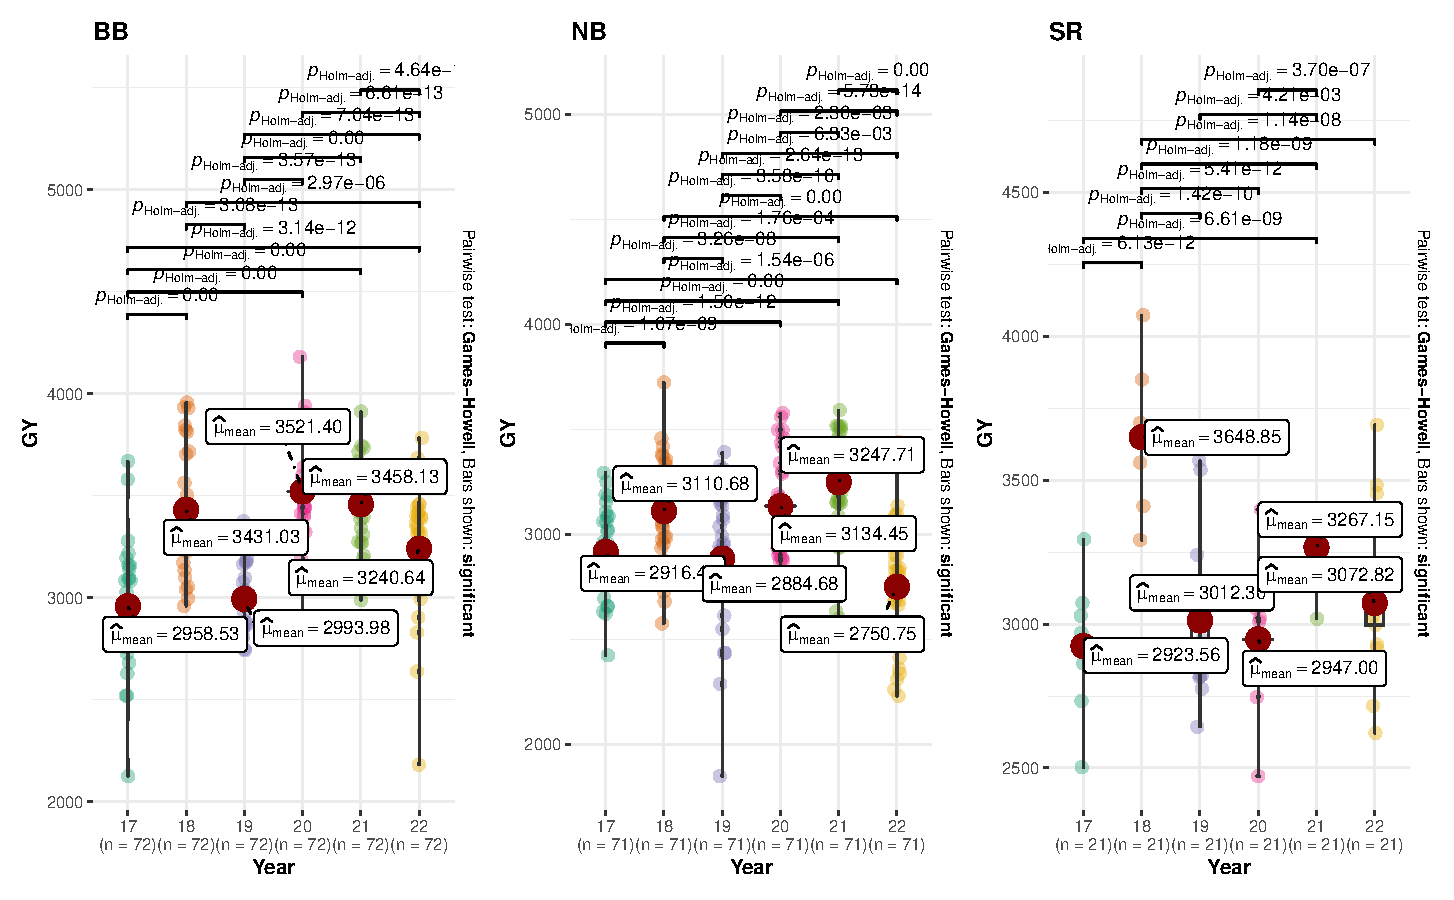
\includegraphics[width=1\linewidth]{figures/plot_ggstatsplot_pred year-1} 

}

\caption{Combination of box and violin plots along with jittered data points for between subjects comparisons by years of grain yield (GY) for black (BB), Navy (NB) and Red (SR) beans. Pairwise Games-Howell test used. Comparisons showing only significant values.}\label{fig:plot_ggstatsplot_pred year}
\end{figure}

\begin{Shaded}
\begin{Highlighting}[]
\FunctionTok{str}\NormalTok{(blues\_stage.I)}
\end{Highlighting}
\end{Shaded}

Classes `data.table' and `data.frame': 984 obs. of 5 variables: \$ year
: Factor w/ 6 levels ``17'',``18'',``19'',..: 1 1 1 1 1 1 1 1 1 1
\ldots{} \$ name : chr ``B1'' ``B10'' ``B11'' ``B12'' \ldots{} \$ mkt :
chr ``BB'' ``BB'' ``BB'' ``BB'' \ldots{} \$ se : num 141.3 98.7 113.8
113.8 355.7 \ldots{} \$ yield: num 2727 3579 2947 3092 2959 \ldots{} -
attr(*, ``.internal.selfref'')=

\begin{Shaded}
\begin{Highlighting}[]
\NormalTok{blues\_stage.I}\SpecialCharTok{$}\NormalTok{year }\OtherTok{\textless{}{-}} \FunctionTok{as.numeric}\NormalTok{(blues\_stage.I}\SpecialCharTok{$}\NormalTok{year)}

\NormalTok{blues\_stage.I}\SpecialCharTok{$}\NormalTok{year[blues\_stage.I}\SpecialCharTok{$}\NormalTok{year }\SpecialCharTok{==} \DecValTok{1}\NormalTok{]}\OtherTok{\textless{}{-}} \DecValTok{17}
\NormalTok{blues\_stage.I}\SpecialCharTok{$}\NormalTok{year[blues\_stage.I}\SpecialCharTok{$}\NormalTok{year }\SpecialCharTok{==} \DecValTok{2}\NormalTok{]}\OtherTok{\textless{}{-}} \DecValTok{18}
\NormalTok{blues\_stage.I}\SpecialCharTok{$}\NormalTok{year[blues\_stage.I}\SpecialCharTok{$}\NormalTok{year }\SpecialCharTok{==} \DecValTok{3}\NormalTok{]}\OtherTok{\textless{}{-}} \DecValTok{19}
\NormalTok{blues\_stage.I}\SpecialCharTok{$}\NormalTok{year[blues\_stage.I}\SpecialCharTok{$}\NormalTok{year }\SpecialCharTok{==} \DecValTok{4}\NormalTok{]}\OtherTok{\textless{}{-}} \DecValTok{20}
\NormalTok{blues\_stage.I}\SpecialCharTok{$}\NormalTok{year[blues\_stage.I}\SpecialCharTok{$}\NormalTok{year }\SpecialCharTok{==} \DecValTok{5}\NormalTok{]}\OtherTok{\textless{}{-}} \DecValTok{21}
\NormalTok{blues\_stage.I}\SpecialCharTok{$}\NormalTok{year[blues\_stage.I}\SpecialCharTok{$}\NormalTok{year }\SpecialCharTok{==} \DecValTok{6}\NormalTok{]}\OtherTok{\textless{}{-}} \DecValTok{22}
\end{Highlighting}
\end{Shaded}

\begin{Shaded}
\begin{Highlighting}[]
\NormalTok{beans\_desc }\OtherTok{\textless{}{-}} \FunctionTok{desc\_stat}\NormalTok{(blues\_stage.I, yield, }\AttributeTok{stats =}\NormalTok{ (}\StringTok{"ci.t, hmean, n, se"}\NormalTok{), }\AttributeTok{by =}\NormalTok{ mkt)}
\CommentTok{\#print(beans\_desc)}

\NormalTok{beans\_desc}\OtherTok{\textless{}{-}}\NormalTok{beans\_desc[}\SpecialCharTok{{-}}\FunctionTok{c}\NormalTok{(}\DecValTok{2}\NormalTok{)]}

\FunctionTok{colnames}\NormalTok{(beans\_desc)}\OtherTok{\textless{}{-}} \FunctionTok{c}\NormalTok{(}\StringTok{"MKT"}\NormalTok{,}\StringTok{"CI"}\NormalTok{, }\StringTok{"Mean"}\NormalTok{, }\StringTok{"N"}\NormalTok{, }\StringTok{"SE"}\NormalTok{)}

\NormalTok{beans\_desc}\OtherTok{\textless{}{-}}\FunctionTok{data.frame}\NormalTok{(beans\_desc, }\AttributeTok{row.names =}\NormalTok{T)}

\CommentTok{\#rownames(beans\_desc) \textless{}{-} NULL}
\end{Highlighting}
\end{Shaded}

\begin{figure}[H]

{\centering 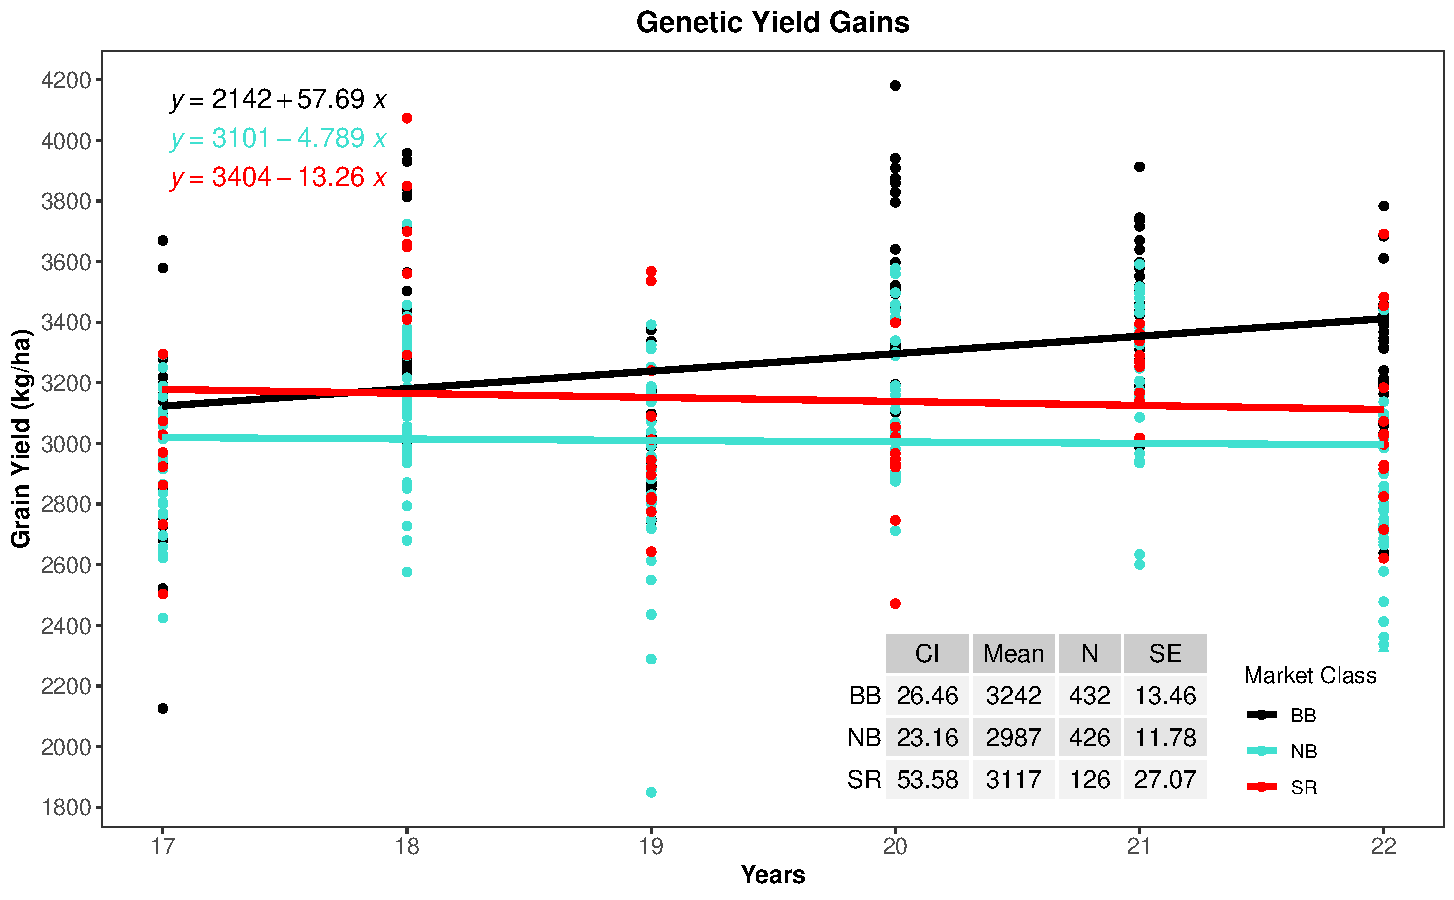
\includegraphics[width=1\linewidth]{figures/plot_year_gains-1} 

}

\caption{Combination of box and violin plots along with jittered data points for between subjects comparisons by years of grain yield (GY) for black (BB), Navy (NB) and Red (SR) beans. Pairwise Games-Howell test used. Comparisons showing significant values only.}\label{fig:plot_year_gains}
\end{figure}

\hypertarget{two-stage-mixed-model-analysis}{%
\subsection{Two Stage mixed model
analysis}\label{two-stage-mixed-model-analysis}}

The following pipeline will be used: 1-Stage = BLUEs estimation for the
vector of the variable GY in the ith genotype, and jth year within
\texttt{loc}. Then the BLUEs from the 1-Stage (Yik) will be used to
predict the BLUPs (Yijl) of the ith genotype in the lth location and jth
rep in the 2-Stage in which this second model have \texttt{name} and
\texttt{loc} effects as random.

\hypertarget{st-stage-mixed-model-analysis}{%
\subsubsection{1st Stage mixed model
analysis}\label{st-stage-mixed-model-analysis}}

\begin{Shaded}
\begin{Highlighting}[]
\CommentTok{\#rm(list=ls())}
\NormalTok{data\_beans }\OtherTok{=} \FunctionTok{read.csv}\NormalTok{(}\StringTok{"data/DataBean\_MET\_GYv2.csv"}\NormalTok{,}\AttributeTok{h=}\NormalTok{T, }\AttributeTok{stringsAsFactors =}\NormalTok{ T)}
\CommentTok{\#str(data\_beans)}
\CommentTok{\# Data adjustment}
\CommentTok{\# All the effect columns must be as a factor to run in ASReml{-}r.}
\NormalTok{cols }\OtherTok{\textless{}{-}} \FunctionTok{c}\NormalTok{(}\StringTok{"rep"}\NormalTok{, }\StringTok{"name"}\NormalTok{, }\StringTok{"loc"}\NormalTok{,}\StringTok{"year"}\NormalTok{, }\StringTok{"mkt"}\NormalTok{, }\StringTok{"year\_loc"}\NormalTok{)}
\NormalTok{data\_beans[cols] }\OtherTok{\textless{}{-}} \FunctionTok{lapply}\NormalTok{(data\_beans[cols], factor)}
\NormalTok{data\_beans }\OtherTok{\textless{}{-}} \FunctionTok{data.table}\NormalTok{(data\_beans)}
\end{Highlighting}
\end{Shaded}

The BLUES will be estimated using a mixed-effect model. The BLUEs will
be obtained by location using a loop with \texttt{ASReml} and storage
into the list.

The following mixed model was used to estimate the BLUEs of each
genotype within location with one value per genotype per experiment and
rep, for the first step (random effects are underlined in all
equations):

\[
\underline{Y_{ik}} = \mu  + {G_i} + \underline{S_{k}} + \underline{GS_{ik}} + \underline{\varepsilon_{ik}} 
\]

where \(Y_{ik}\) is the observed yield in the \emph{i}th genotype and
\emph{k}th year, \(\mu\) is the overall mean, \(G_i\) is the effect of
the \emph{i}th genotype, \(S_{k}\) is the effect of the \emph{k}th year,
\(GS_{ik}\) is the effect of the interaction between the ith genotype
and the kth year, and \(\varepsilon_{ik}\) are the residual, with
\(S_{k}\)\textasciitilde N(0,\(\sigma_{Y}^{2}\)),
\(GS_{ik}\)\textasciitilde N(0,\(\sigma_{Y}^{2}\)), and
\(\varepsilon_{ik}\)\textasciitilde N(0,\(\sigma_{\varepsilon}^{2}\)),
all independent, where \(\sigma_{Y}^{2}\) is the year variance, and
\(\sigma_{\varepsilon}^{2}\) is the mean error variance across
experiments.

\begin{verbatim}
#> `summarise()` has grouped output by 'name'. You can override using the `.groups` argument.
#> `summarise()` has grouped output by 'name'. You can override using the `.groups` argument.
#> `summarise()` has grouped output by 'name'. You can override using the `.groups` argument.
#> `summarise()` has grouped output by 'name'. You can override using the `.groups` argument.
#> `summarise()` has grouped output by 'name'. You can override using the `.groups` argument.
#> `summarise()` has grouped output by 'name'. You can override using the `.groups` argument.
#> `summarise()` has grouped output by 'name'. You can override using the `.groups` argument.
#> `summarise()` has grouped output by 'name'. You can override using the `.groups` argument.
#> `summarise()` has grouped output by 'name'. You can override using the `.groups` argument.
#> `summarise()` has grouped output by 'name'. You can override using the `.groups` argument.
#> `summarise()` has grouped output by 'name'. You can override using the `.groups` argument.
#> `summarise()` has grouped output by 'name'. You can override using the `.groups` argument.
\end{verbatim}

\begin{Shaded}
\begin{Highlighting}[]
\DocumentationTok{\#\# Loop to get the year effect corrected by year}
\DocumentationTok{\#\# Only genotypes present in years}

\CommentTok{\#str(data\_beans)}
\NormalTok{data\_beans}\SpecialCharTok{$}\NormalTok{var\_years }\OtherTok{\textless{}{-}} \FunctionTok{as.factor}\NormalTok{(data\_beans}\SpecialCharTok{$}\NormalTok{var\_years)}
\NormalTok{year }\OtherTok{\textless{}{-}} \FunctionTok{nlevels}\NormalTok{(data\_beans}\SpecialCharTok{$}\NormalTok{var\_years)}

\NormalTok{data\_beans\_group}\OtherTok{\textless{}{-}}\NormalTok{ data\_beans}
\DocumentationTok{\#\# Analysis per site and mkt class}
\CommentTok{\#mkt\_n \textless{}{-} levels(data\_beans$mkt)}

\NormalTok{Envs }\OtherTok{\textless{}{-}} \FunctionTok{levels}\NormalTok{(data\_beans}\SpecialCharTok{$}\NormalTok{loc)}

\NormalTok{stgI\_list }\OtherTok{\textless{}{-}} \FunctionTok{matrix}\NormalTok{(}\AttributeTok{data=}\FunctionTok{list}\NormalTok{(), }\AttributeTok{nrow=}\FunctionTok{length}\NormalTok{(Envs), }\AttributeTok{ncol=}\DecValTok{1}\NormalTok{,}
                    \AttributeTok{dimnames=}\FunctionTok{list}\NormalTok{(Envs, }\FunctionTok{c}\NormalTok{(}\StringTok{"BLUES"}\NormalTok{)))}

\NormalTok{mkt }\OtherTok{\textless{}{-}} \FunctionTok{nlevels}\NormalTok{(data\_beans}\SpecialCharTok{$}\NormalTok{mkt)}

\ControlFlowTok{for}\NormalTok{ (y }\ControlFlowTok{in} \DecValTok{1}\SpecialCharTok{:}\NormalTok{year) \{}

\NormalTok{  by }\OtherTok{\textless{}{-}} \FunctionTok{levels}\NormalTok{(data\_beans}\SpecialCharTok{$}\NormalTok{var\_years)}
\NormalTok{  cy }\OtherTok{\textless{}{-}}\NormalTok{ by[y]}
  
\NormalTok{  data\_beans\_temp1 }\OtherTok{\textless{}{-}} \FunctionTok{droplevels}\NormalTok{(}\FunctionTok{subset}\NormalTok{(data\_beans, var\_years}\SpecialCharTok{==}\NormalTok{cy))}
  
\ControlFlowTok{if}\NormalTok{(y }\SpecialCharTok{==} \DecValTok{1}\NormalTok{) \{}\ControlFlowTok{next}

\NormalTok{\}}\ControlFlowTok{else}\NormalTok{ \{ }
  
  \ControlFlowTok{for}\NormalTok{(k }\ControlFlowTok{in} \DecValTok{1}\SpecialCharTok{:}\NormalTok{mkt)\{}

\NormalTok{  bk }\OtherTok{\textless{}{-}} \FunctionTok{levels}\NormalTok{(data\_beans\_temp1}\SpecialCharTok{$}\NormalTok{mkt)}
\NormalTok{  cj }\OtherTok{\textless{}{-}}\NormalTok{ bk[k]}
  \CommentTok{\#print(cj)}
  
\NormalTok{  data\_beans\_temp2 }\OtherTok{\textless{}{-}} \FunctionTok{droplevels}\NormalTok{(}\FunctionTok{subset}\NormalTok{(data\_beans\_temp1, mkt}\SpecialCharTok{==}\NormalTok{cj))}

  \ControlFlowTok{for}\NormalTok{ (i }\ControlFlowTok{in}\NormalTok{ Envs)\{}
    \CommentTok{\#i=Envs[1]}
\NormalTok{    Edat }\OtherTok{\textless{}{-}} \FunctionTok{droplevels}\NormalTok{(}\FunctionTok{subset}\NormalTok{(data\_beans\_temp2, loc}\SpecialCharTok{==}\NormalTok{i))}
    
    \CommentTok{\#print(i)}
    
\NormalTok{    mod}\FloatTok{.1} \OtherTok{\textless{}{-}} \FunctionTok{asreml}\NormalTok{(}\AttributeTok{fixed       =}\NormalTok{ gy\_kg\_ha }\SpecialCharTok{\textasciitilde{}}\NormalTok{ name}\SpecialCharTok{:}\NormalTok{rep,}
                    \AttributeTok{random      =} \SpecialCharTok{\textasciitilde{}}\NormalTok{ year }\SpecialCharTok{+}\NormalTok{ name}\SpecialCharTok{:}\NormalTok{year ,}
                    \AttributeTok{data        =}\NormalTok{ Edat,}
                \AttributeTok{predict     =} \FunctionTok{predict.asreml}\NormalTok{(}\AttributeTok{classify =} \StringTok{"name:rep"}\NormalTok{,}\AttributeTok{vcov=}\ConstantTok{TRUE}\NormalTok{, }\AttributeTok{aliased =}\NormalTok{ T),}
                    \AttributeTok{trace       =}\NormalTok{ F,}
                    \AttributeTok{maxit       =} \DecValTok{500}\NormalTok{)}
    
   \CommentTok{\# print(summary.asreml(mod.1)$varcomp)}
    \CommentTok{\# wald(mod.1)}

\NormalTok{  blue}\FloatTok{.1}\OtherTok{\textless{}{-}} \FunctionTok{as.data.frame}\NormalTok{((mod}\FloatTok{.1}\SpecialCharTok{$}\NormalTok{predictions}\SpecialCharTok{$}\NormalTok{pvals[}\DecValTok{1}\SpecialCharTok{:}\DecValTok{4}\NormalTok{])) }
  \FunctionTok{names}\NormalTok{(blue}\FloatTok{.1}\NormalTok{) }\OtherTok{\textless{}{-}} \FunctionTok{c}\NormalTok{(}\StringTok{"name"}\NormalTok{, }\StringTok{"rep"}\NormalTok{, }\StringTok{"yield"}\NormalTok{, }\StringTok{"se"}\NormalTok{)}
\NormalTok{  blue}\FloatTok{.1}\SpecialCharTok{$}\NormalTok{mkt}\OtherTok{\textless{}{-}}\NormalTok{ cj}
\NormalTok{  blue}\FloatTok{.1}\SpecialCharTok{$}\NormalTok{var\_years}\OtherTok{\textless{}{-}}\NormalTok{ cy}
  
\NormalTok{    stgI\_list[[i, }\StringTok{"BLUES"}\NormalTok{]] }\OtherTok{\textless{}{-}}\NormalTok{ blue}\FloatTok{.1} \CommentTok{\# put all the results of Stage 1 in the list}
    
    \FunctionTok{rm}\NormalTok{(Edat,mod}\FloatTok{.1}\NormalTok{, blue, blue}\FloatTok{.1}\NormalTok{)}
    
\NormalTok{   \}}
   \ControlFlowTok{if}\NormalTok{(k}\SpecialCharTok{==}\DecValTok{1}\NormalTok{)\{stgI\_list}\FloatTok{.1}\OtherTok{\textless{}{-}}\NormalTok{stgI\_list\}}\ControlFlowTok{else}\NormalTok{\{stgI\_list}\FloatTok{.1}\OtherTok{\textless{}{-}}\FunctionTok{rbind}\NormalTok{(stgI\_list}\FloatTok{.1}\NormalTok{, stgI\_list)\}}
   
\NormalTok{\}}
\NormalTok{\}}
  \ControlFlowTok{if}\NormalTok{(y}\SpecialCharTok{==}\DecValTok{2}\NormalTok{)\{stgI\_list}\FloatTok{.2}\OtherTok{\textless{}{-}}\NormalTok{stgI\_list}\FloatTok{.1}\NormalTok{\}}\ControlFlowTok{else}\NormalTok{\{stgI\_list}\FloatTok{.2}\OtherTok{\textless{}{-}}\FunctionTok{rbind}\NormalTok{(stgI\_list}\FloatTok{.2}\NormalTok{, stgI\_list}\FloatTok{.1}\NormalTok{)\}}
  
\NormalTok{\}}
\end{Highlighting}
\end{Shaded}

\hypertarget{preparing-dataset-of-stage-i-for-stage-ii}{%
\paragraph{Preparing dataset of Stage I for Stage
II}\label{preparing-dataset-of-stage-i-for-stage-ii}}

Merging the original data to have all the factors in the final table
with: \texttt{name}, \texttt{loc}, \texttt{mkt}, \texttt{rep}

\begin{Shaded}
\begin{Highlighting}[]
\DocumentationTok{\#\#\#\#\# Unlist the results of Stage I and format as data.table \#\#\#\#\#}
\NormalTok{blues\_stageI }\OtherTok{\textless{}{-}} \FunctionTok{data.table}\NormalTok{(}\FunctionTok{ldply}\NormalTok{(stgI\_list}\FloatTok{.2}\NormalTok{[, }\StringTok{"BLUES"}\NormalTok{], data.frame, }\AttributeTok{.id=}\StringTok{"loc"}\NormalTok{))}

\NormalTok{blues\_stage.I }\OtherTok{\textless{}{-}}\NormalTok{ blues\_stageI[}\FunctionTok{order}\NormalTok{(blues\_stageI}\SpecialCharTok{$}\NormalTok{loc,blues\_stageI}\SpecialCharTok{$}\NormalTok{name),]}

\NormalTok{blues\_stage.I.SEmean }\OtherTok{\textless{}{-}}\NormalTok{ blues\_stage.I }\SpecialCharTok{\%\textgreater{}\%}
\NormalTok{  dplyr}\SpecialCharTok{::}\FunctionTok{summarise}\NormalTok{(}\AttributeTok{Mean\_SE =} \FunctionTok{mean}\NormalTok{(se, }\AttributeTok{na.rm =} \ConstantTok{TRUE}\NormalTok{))}

\FunctionTok{print}\NormalTok{(blues\_stage.I.SEmean)}
\end{Highlighting}
\end{Shaded}

Mean\_SE 1 440.9

\begin{Shaded}
\begin{Highlighting}[]
\CommentTok{\#str(blues\_stage.I)}
\end{Highlighting}
\end{Shaded}

\begin{Shaded}
\begin{Highlighting}[]
\CommentTok{\# Change the order of columns}
\NormalTok{blues\_stage.I }\OtherTok{\textless{}{-}}\NormalTok{ blues\_stage.I }\SpecialCharTok{\%\textgreater{}\%} 
\NormalTok{  dplyr}\SpecialCharTok{::}\FunctionTok{select}\NormalTok{(loc, name, rep, mkt, yield)}
\end{Highlighting}
\end{Shaded}

\hypertarget{nd-stage-mixed-model-analysis}{%
\subsubsection{2nd Stage mixed model
analysis}\label{nd-stage-mixed-model-analysis}}

The following linear mixed model with interaction effect will be used in
the 2-Stage in order to investigate the multi-environment trials (MET)
as follow:

\[
\underline{Y_{ijl}} = \mu  + \underline{G_i} + {E_{l}} + \beta_{jl} + \underline{GE_{il}} + \underline{\varepsilon_{ijl}} 
\]

where \({Y_{ijl}}\) is the response variable (e.g., grain yield)
observed in the \emph{j}th repetion of the \emph{i}th genotype in the
\emph{l}th location (\emph{i} = 1, 2, \ldots, \emph{g}; \emph{j} = 1, 2,
\ldots, \emph{b}; \emph{l} = 1, 2, \ldots, \emph{e}); \(\mu\) is the
grand mean; \(\underline{G_i}\) is the effect of the \emph{i}th
genotype; \(E_l\) is the effect of the \emph{l}th location (env);
\(\beta_{jl}\) is the effect of the \emph{j}th rep with the \emph{l}th
location; \(\underline{GE_{il}}\) is the interaction effect of the
\emph{i}th genotype nested within the \emph{l}th location; and
\(\mathop \varepsilon \nolimits_{ijl}\) is the random error, in witch
with \(G_{i}\)\textasciitilde N(0,\(\sigma_{G}^{2}\)),
\(GE_{il}\)\textasciitilde N(0,\(\sigma_{GE}^{2}\)), and
\(\varepsilon_{ijl}\)\textasciitilde N(0,\(\sigma_{\varepsilon}^{2}\)),
all independent, where \(G_{G}^{2}\) is the genotype (name)
variance,\(GS_{GE}^{2}\) is the interaction genotype x environment
variance, and \(\sigma_{\varepsilon}^{2}\) is the mean error variance
across experiments.

\hypertarget{by-market-classes}{%
\subsubsection{By market classes}\label{by-market-classes}}

\begin{itemize}
\tightlist
\item
  Getting the files for the individually market classes
\end{itemize}

\begin{Shaded}
\begin{Highlighting}[]
\NormalTok{blues\_stage.I\_BB }\OtherTok{\textless{}{-}} \FunctionTok{droplevels}\NormalTok{(}\FunctionTok{subset}\NormalTok{(blues\_stage.I, mkt}\SpecialCharTok{==}\StringTok{"BB"}\NormalTok{))}
\NormalTok{blues\_stage.I\_NB }\OtherTok{\textless{}{-}} \FunctionTok{droplevels}\NormalTok{(}\FunctionTok{subset}\NormalTok{(blues\_stage.I, mkt}\SpecialCharTok{==}\StringTok{"NB"}\NormalTok{))}
\NormalTok{blues\_stage.I\_SR }\OtherTok{\textless{}{-}} \FunctionTok{droplevels}\NormalTok{(}\FunctionTok{subset}\NormalTok{(blues\_stage.I, mkt}\SpecialCharTok{==}\StringTok{"SR"}\NormalTok{))}
\end{Highlighting}
\end{Shaded}

\begin{Shaded}
\begin{Highlighting}[]
\NormalTok{blues\_stage.I\_table1}\OtherTok{\textless{}{-}}\NormalTok{ blues\_stage.I }\SpecialCharTok{\%\textgreater{}\%} 
  \FunctionTok{group\_by}\NormalTok{(loc, rep, mkt) }\SpecialCharTok{\%\textgreater{}\%} 
\NormalTok{  dplyr}\SpecialCharTok{::}\FunctionTok{summarise}\NormalTok{(}\AttributeTok{count =} \FunctionTok{length}\NormalTok{(name)) }

\NormalTok{blues\_stage.I\_table1}\OtherTok{\textless{}{-}}\NormalTok{ blues\_stage.I\_table1[,}\DecValTok{3}\SpecialCharTok{:}\DecValTok{4}\NormalTok{]}
\NormalTok{blues\_stage.I\_table1}\OtherTok{\textless{}{-}}\NormalTok{ blues\_stage.I\_table1[}\DecValTok{1}\SpecialCharTok{:}\DecValTok{3}\NormalTok{,]}

\NormalTok{blues\_stage.I\_table1}
\end{Highlighting}
\end{Shaded}

\global\setlength{\Oldarrayrulewidth}{\arrayrulewidth}

\global\setlength{\Oldtabcolsep}{\tabcolsep}

\setlength{\tabcolsep}{0pt}

\renewcommand*{\arraystretch}{1.5}



\providecommand{\ascline}[3]{\noalign{\global\arrayrulewidth #1}\arrayrulecolor[HTML]{#2}\cline{#3}}

\begin{longtable}[c]{|p{0.75in}|p{0.75in}}



\ascline{1.5pt}{666666}{1-2}

\multicolumn{1}{>{\raggedright}m{\dimexpr 0.75in+0\tabcolsep}}{\textcolor[HTML]{000000}{\fontsize{9}{9}\selectfont{\global\setmainfont{Arial}{\textbf{mkt}}}}} & \multicolumn{1}{>{\raggedleft}m{\dimexpr 0.75in+0\tabcolsep}}{\textcolor[HTML]{000000}{\fontsize{9}{9}\selectfont{\global\setmainfont{Arial}{\textbf{count}}}}} \\

\ascline{0.75pt}{666666}{1-2}



\multicolumn{1}{>{\raggedright}m{\dimexpr 0.75in+0\tabcolsep}}{\textcolor[HTML]{999999}{\fontsize{9}{9}\selectfont{\global\setmainfont{Arial}{\textbf{factor}}}}} & \multicolumn{1}{>{\raggedleft}m{\dimexpr 0.75in+0\tabcolsep}}{\textcolor[HTML]{999999}{\fontsize{9}{9}\selectfont{\global\setmainfont{Arial}{\textbf{integer}}}}} \\

\ascline{1.5pt}{666666}{1-2}\endfirsthead

\ascline{1.5pt}{666666}{1-2}

\multicolumn{1}{>{\raggedright}m{\dimexpr 0.75in+0\tabcolsep}}{\textcolor[HTML]{000000}{\fontsize{9}{9}\selectfont{\global\setmainfont{Arial}{\textbf{mkt}}}}} & \multicolumn{1}{>{\raggedleft}m{\dimexpr 0.75in+0\tabcolsep}}{\textcolor[HTML]{000000}{\fontsize{9}{9}\selectfont{\global\setmainfont{Arial}{\textbf{count}}}}} \\

\ascline{0.75pt}{666666}{1-2}



\multicolumn{1}{>{\raggedright}m{\dimexpr 0.75in+0\tabcolsep}}{\textcolor[HTML]{999999}{\fontsize{9}{9}\selectfont{\global\setmainfont{Arial}{\textbf{factor}}}}} & \multicolumn{1}{>{\raggedleft}m{\dimexpr 0.75in+0\tabcolsep}}{\textcolor[HTML]{999999}{\fontsize{9}{9}\selectfont{\global\setmainfont{Arial}{\textbf{integer}}}}} \\

\ascline{1.5pt}{666666}{1-2}\endhead



\multicolumn{2}{>{\raggedright}m{\dimexpr 1.5in+2\tabcolsep}}{\textcolor[HTML]{000000}{\fontsize{9}{9}\selectfont{\global\setmainfont{Arial}{n:\ 3}}}} \\

\ascline{0.75pt}{666666}{1-2}\endfoot



\multicolumn{1}{>{\raggedright}m{\dimexpr 0.75in+0\tabcolsep}}{\textcolor[HTML]{000000}{\fontsize{9}{9}\selectfont{\global\setmainfont{Arial}{BB}}}} & \multicolumn{1}{>{\raggedleft}m{\dimexpr 0.75in+0\tabcolsep}}{\textcolor[HTML]{000000}{\fontsize{9}{9}\selectfont{\global\setmainfont{Arial}{72}}}} \\

\ascline{0.75pt}{666666}{1-2}



\multicolumn{1}{>{\raggedright}m{\dimexpr 0.75in+0\tabcolsep}}{\textcolor[HTML]{000000}{\fontsize{9}{9}\selectfont{\global\setmainfont{Arial}{NB}}}} & \multicolumn{1}{>{\raggedleft}m{\dimexpr 0.75in+0\tabcolsep}}{\textcolor[HTML]{000000}{\fontsize{9}{9}\selectfont{\global\setmainfont{Arial}{71}}}} \\

\ascline{0.75pt}{666666}{1-2}



\multicolumn{1}{>{\raggedright}m{\dimexpr 0.75in+0\tabcolsep}}{\textcolor[HTML]{000000}{\fontsize{9}{9}\selectfont{\global\setmainfont{Arial}{SR}}}} & \multicolumn{1}{>{\raggedleft}m{\dimexpr 0.75in+0\tabcolsep}}{\textcolor[HTML]{000000}{\fontsize{9}{9}\selectfont{\global\setmainfont{Arial}{21}}}} \\

\ascline{1.5pt}{666666}{1-2}



\end{longtable}



\arrayrulecolor[HTML]{000000}

\global\setlength{\arrayrulewidth}{\Oldarrayrulewidth}

\global\setlength{\tabcolsep}{\Oldtabcolsep}

\renewcommand*{\arraystretch}{1}

\begin{Shaded}
\begin{Highlighting}[]
\FunctionTok{str}\NormalTok{(blues\_stage.I\_BB)}
\end{Highlighting}
\end{Shaded}

Classes `data.table' and `data.frame': 1152 obs. of 5 variables: \$ loc
: Factor w/ 4 levels ``BA'',``HU'',``SA'',..: 1 1 1 1 1 1 1 1 1 1
\ldots{} \$ name : Factor w/ 72 levels ``B1'',``B10'',``B13'',..: 1 1 1
1 2 2 2 2 3 3 \ldots{} \$ rep : Factor w/ 4 levels
``1'',``2'',``3'',``4'': 1 2 3 4 1 2 3 4 1 2 \ldots{} \$ mkt : Factor w/
1 level ``BB'': 1 1 1 1 1 1 1 1 1 1 \ldots{} \$ yield: num 2350 3148
2348 1753 3433 \ldots{} - attr(*, ``.internal.selfref'')=

\begin{Shaded}
\begin{Highlighting}[]
\ControlFlowTok{if}\NormalTok{ (knitr}\SpecialCharTok{::}\FunctionTok{is\_html\_output}\NormalTok{()) \{}

  \FunctionTok{print\_table}\NormalTok{(blues\_stage.I\_BB)}
  
\NormalTok{\}}\ControlFlowTok{else}\NormalTok{\{}

\FunctionTok{flextable}\NormalTok{(}\FunctionTok{head}\NormalTok{(blues\_stage.I\_BB)) }\SpecialCharTok{\%\textgreater{}\%} 
   \FunctionTok{add\_footer\_lines}\NormalTok{(}
     \FunctionTok{c}\NormalTok{(}\StringTok{"Black beans data set"}\NormalTok{, }
       \StringTok{"Header data set showing the 6 first entry"}\NormalTok{)) }\SpecialCharTok{\%\textgreater{}\%} 
   \FunctionTok{autofit}\NormalTok{() }\SpecialCharTok{\%\textgreater{}\%} 
   \FunctionTok{add\_header\_lines}\NormalTok{(}\StringTok{"Dry Beans varieties trial"}\NormalTok{) }\SpecialCharTok{\%\textgreater{}\%} 
  \FunctionTok{theme\_design2}\NormalTok{()}
\NormalTok{\}}
\end{Highlighting}
\end{Shaded}

\global\setlength{\Oldarrayrulewidth}{\arrayrulewidth}

\global\setlength{\Oldtabcolsep}{\tabcolsep}

\setlength{\tabcolsep}{0pt}

\renewcommand*{\arraystretch}{1.5}



\providecommand{\ascline}[3]{\noalign{\global\arrayrulewidth #1}\arrayrulecolor[HTML]{#2}\cline{#3}}

\begin{longtable}[c]{|p{0.75in}|p{0.75in}|p{0.75in}|p{0.75in}|p{0.75in}}



\ascline{1.5pt}{666666}{1-5}

\multicolumn{5}{>{\raggedright}m{\dimexpr 3.75in+8\tabcolsep}}{\textcolor[HTML]{000000}{\fontsize{10}{10}\selectfont{\global\setmainfont{Arial}{\textbf{Dry\ Beans\ varieties\ trial}}}}} \\

\ascline{0.75pt}{666666}{1-5}



\multicolumn{1}{>{\raggedright}m{\dimexpr 0.75in+0\tabcolsep}}{\textcolor[HTML]{000000}{\fontsize{10}{10}\selectfont{\global\setmainfont{Arial}{\textbf{loc}}}}} & \multicolumn{1}{>{\raggedright}m{\dimexpr 0.75in+0\tabcolsep}}{\textcolor[HTML]{000000}{\fontsize{10}{10}\selectfont{\global\setmainfont{Arial}{\textbf{name}}}}} & \multicolumn{1}{>{\raggedright}m{\dimexpr 0.75in+0\tabcolsep}}{\textcolor[HTML]{000000}{\fontsize{10}{10}\selectfont{\global\setmainfont{Arial}{\textbf{rep}}}}} & \multicolumn{1}{>{\raggedright}m{\dimexpr 0.75in+0\tabcolsep}}{\textcolor[HTML]{000000}{\fontsize{10}{10}\selectfont{\global\setmainfont{Arial}{\textbf{mkt}}}}} & \multicolumn{1}{>{\raggedleft}m{\dimexpr 0.75in+0\tabcolsep}}{\textcolor[HTML]{000000}{\fontsize{10}{10}\selectfont{\global\setmainfont{Arial}{\textbf{yield}}}}} \\

\ascline{1.5pt}{666666}{1-5}\endfirsthead

\ascline{1.5pt}{666666}{1-5}

\multicolumn{5}{>{\raggedright}m{\dimexpr 3.75in+8\tabcolsep}}{\textcolor[HTML]{000000}{\fontsize{10}{10}\selectfont{\global\setmainfont{Arial}{\textbf{Dry\ Beans\ varieties\ trial}}}}} \\

\ascline{0.75pt}{666666}{1-5}



\multicolumn{1}{>{\raggedright}m{\dimexpr 0.75in+0\tabcolsep}}{\textcolor[HTML]{000000}{\fontsize{10}{10}\selectfont{\global\setmainfont{Arial}{\textbf{loc}}}}} & \multicolumn{1}{>{\raggedright}m{\dimexpr 0.75in+0\tabcolsep}}{\textcolor[HTML]{000000}{\fontsize{10}{10}\selectfont{\global\setmainfont{Arial}{\textbf{name}}}}} & \multicolumn{1}{>{\raggedright}m{\dimexpr 0.75in+0\tabcolsep}}{\textcolor[HTML]{000000}{\fontsize{10}{10}\selectfont{\global\setmainfont{Arial}{\textbf{rep}}}}} & \multicolumn{1}{>{\raggedright}m{\dimexpr 0.75in+0\tabcolsep}}{\textcolor[HTML]{000000}{\fontsize{10}{10}\selectfont{\global\setmainfont{Arial}{\textbf{mkt}}}}} & \multicolumn{1}{>{\raggedleft}m{\dimexpr 0.75in+0\tabcolsep}}{\textcolor[HTML]{000000}{\fontsize{10}{10}\selectfont{\global\setmainfont{Arial}{\textbf{yield}}}}} \\

\ascline{1.5pt}{666666}{1-5}\endhead



\multicolumn{5}{>{\raggedright}m{\dimexpr 3.75in+8\tabcolsep}}{\textcolor[HTML]{000000}{\fontsize{8}{8}\selectfont{\global\setmainfont{Arial}{Black\ beans\ data\ set}}}} \\

\ascline{0.75pt}{666666}{1-5}



\multicolumn{5}{>{\raggedright}m{\dimexpr 3.75in+8\tabcolsep}}{\textcolor[HTML]{000000}{\fontsize{8}{8}\selectfont{\global\setmainfont{Arial}{Header\ data\ set\ showing\ the\ 6\ first\ entry}}}} \\

\ascline{0.75pt}{666666}{1-5}\endfoot



\multicolumn{1}{>{\raggedright}m{\dimexpr 0.75in+0\tabcolsep}}{\textcolor[HTML]{000000}{\fontsize{9}{9}\selectfont{\global\setmainfont{Arial}{BA}}}} & \multicolumn{1}{>{\raggedright}m{\dimexpr 0.75in+0\tabcolsep}}{\textcolor[HTML]{000000}{\fontsize{9}{9}\selectfont{\global\setmainfont{Arial}{B1}}}} & \multicolumn{1}{>{\raggedright}m{\dimexpr 0.75in+0\tabcolsep}}{\textcolor[HTML]{000000}{\fontsize{9}{9}\selectfont{\global\setmainfont{Arial}{1}}}} & \multicolumn{1}{>{\raggedright}m{\dimexpr 0.75in+0\tabcolsep}}{\textcolor[HTML]{000000}{\fontsize{9}{9}\selectfont{\global\setmainfont{Arial}{BB}}}} & \multicolumn{1}{>{\raggedleft}m{\dimexpr 0.75in+0\tabcolsep}}{\textcolor[HTML]{000000}{\fontsize{9}{9}\selectfont{\global\setmainfont{Arial}{2,350}}}} \\

\ascline{0.75pt}{666666}{1-5}



\multicolumn{1}{>{\raggedright}m{\dimexpr 0.75in+0\tabcolsep}}{\textcolor[HTML]{000000}{\fontsize{9}{9}\selectfont{\global\setmainfont{Arial}{BA}}}} & \multicolumn{1}{>{\raggedright}m{\dimexpr 0.75in+0\tabcolsep}}{\textcolor[HTML]{000000}{\fontsize{9}{9}\selectfont{\global\setmainfont{Arial}{B1}}}} & \multicolumn{1}{>{\raggedright}m{\dimexpr 0.75in+0\tabcolsep}}{\textcolor[HTML]{000000}{\fontsize{9}{9}\selectfont{\global\setmainfont{Arial}{2}}}} & \multicolumn{1}{>{\raggedright}m{\dimexpr 0.75in+0\tabcolsep}}{\textcolor[HTML]{000000}{\fontsize{9}{9}\selectfont{\global\setmainfont{Arial}{BB}}}} & \multicolumn{1}{>{\raggedleft}m{\dimexpr 0.75in+0\tabcolsep}}{\textcolor[HTML]{000000}{\fontsize{9}{9}\selectfont{\global\setmainfont{Arial}{3,148}}}} \\

\ascline{0.75pt}{666666}{1-5}



\multicolumn{1}{>{\raggedright}m{\dimexpr 0.75in+0\tabcolsep}}{\textcolor[HTML]{000000}{\fontsize{9}{9}\selectfont{\global\setmainfont{Arial}{BA}}}} & \multicolumn{1}{>{\raggedright}m{\dimexpr 0.75in+0\tabcolsep}}{\textcolor[HTML]{000000}{\fontsize{9}{9}\selectfont{\global\setmainfont{Arial}{B1}}}} & \multicolumn{1}{>{\raggedright}m{\dimexpr 0.75in+0\tabcolsep}}{\textcolor[HTML]{000000}{\fontsize{9}{9}\selectfont{\global\setmainfont{Arial}{3}}}} & \multicolumn{1}{>{\raggedright}m{\dimexpr 0.75in+0\tabcolsep}}{\textcolor[HTML]{000000}{\fontsize{9}{9}\selectfont{\global\setmainfont{Arial}{BB}}}} & \multicolumn{1}{>{\raggedleft}m{\dimexpr 0.75in+0\tabcolsep}}{\textcolor[HTML]{000000}{\fontsize{9}{9}\selectfont{\global\setmainfont{Arial}{2,348}}}} \\

\ascline{0.75pt}{666666}{1-5}



\multicolumn{1}{>{\raggedright}m{\dimexpr 0.75in+0\tabcolsep}}{\textcolor[HTML]{000000}{\fontsize{9}{9}\selectfont{\global\setmainfont{Arial}{BA}}}} & \multicolumn{1}{>{\raggedright}m{\dimexpr 0.75in+0\tabcolsep}}{\textcolor[HTML]{000000}{\fontsize{9}{9}\selectfont{\global\setmainfont{Arial}{B1}}}} & \multicolumn{1}{>{\raggedright}m{\dimexpr 0.75in+0\tabcolsep}}{\textcolor[HTML]{000000}{\fontsize{9}{9}\selectfont{\global\setmainfont{Arial}{4}}}} & \multicolumn{1}{>{\raggedright}m{\dimexpr 0.75in+0\tabcolsep}}{\textcolor[HTML]{000000}{\fontsize{9}{9}\selectfont{\global\setmainfont{Arial}{BB}}}} & \multicolumn{1}{>{\raggedleft}m{\dimexpr 0.75in+0\tabcolsep}}{\textcolor[HTML]{000000}{\fontsize{9}{9}\selectfont{\global\setmainfont{Arial}{1,753}}}} \\

\ascline{0.75pt}{666666}{1-5}



\multicolumn{1}{>{\raggedright}m{\dimexpr 0.75in+0\tabcolsep}}{\textcolor[HTML]{000000}{\fontsize{9}{9}\selectfont{\global\setmainfont{Arial}{BA}}}} & \multicolumn{1}{>{\raggedright}m{\dimexpr 0.75in+0\tabcolsep}}{\textcolor[HTML]{000000}{\fontsize{9}{9}\selectfont{\global\setmainfont{Arial}{B10}}}} & \multicolumn{1}{>{\raggedright}m{\dimexpr 0.75in+0\tabcolsep}}{\textcolor[HTML]{000000}{\fontsize{9}{9}\selectfont{\global\setmainfont{Arial}{1}}}} & \multicolumn{1}{>{\raggedright}m{\dimexpr 0.75in+0\tabcolsep}}{\textcolor[HTML]{000000}{\fontsize{9}{9}\selectfont{\global\setmainfont{Arial}{BB}}}} & \multicolumn{1}{>{\raggedleft}m{\dimexpr 0.75in+0\tabcolsep}}{\textcolor[HTML]{000000}{\fontsize{9}{9}\selectfont{\global\setmainfont{Arial}{3,433}}}} \\

\ascline{0.75pt}{666666}{1-5}



\multicolumn{1}{>{\raggedright}m{\dimexpr 0.75in+0\tabcolsep}}{\textcolor[HTML]{000000}{\fontsize{9}{9}\selectfont{\global\setmainfont{Arial}{BA}}}} & \multicolumn{1}{>{\raggedright}m{\dimexpr 0.75in+0\tabcolsep}}{\textcolor[HTML]{000000}{\fontsize{9}{9}\selectfont{\global\setmainfont{Arial}{B10}}}} & \multicolumn{1}{>{\raggedright}m{\dimexpr 0.75in+0\tabcolsep}}{\textcolor[HTML]{000000}{\fontsize{9}{9}\selectfont{\global\setmainfont{Arial}{2}}}} & \multicolumn{1}{>{\raggedright}m{\dimexpr 0.75in+0\tabcolsep}}{\textcolor[HTML]{000000}{\fontsize{9}{9}\selectfont{\global\setmainfont{Arial}{BB}}}} & \multicolumn{1}{>{\raggedleft}m{\dimexpr 0.75in+0\tabcolsep}}{\textcolor[HTML]{000000}{\fontsize{9}{9}\selectfont{\global\setmainfont{Arial}{3,170}}}} \\

\ascline{1.5pt}{666666}{1-5}



\end{longtable}



\arrayrulecolor[HTML]{000000}

\global\setlength{\arrayrulewidth}{\Oldarrayrulewidth}

\global\setlength{\tabcolsep}{\Oldtabcolsep}

\renewcommand*{\arraystretch}{1}

\begin{Shaded}
\begin{Highlighting}[]
\ControlFlowTok{if}\NormalTok{ (knitr}\SpecialCharTok{::}\FunctionTok{is\_html\_output}\NormalTok{()) \{}

  \FunctionTok{print\_table}\NormalTok{(blues\_stage.I\_NB)}
  
\NormalTok{\}}\ControlFlowTok{else}\NormalTok{\{}
  
\FunctionTok{flextable}\NormalTok{(}\FunctionTok{head}\NormalTok{(blues\_stage.I\_NB)) }\SpecialCharTok{\%\textgreater{}\%} 
   \FunctionTok{add\_footer\_lines}\NormalTok{(}
     \FunctionTok{c}\NormalTok{(}\StringTok{"Navy beans data set"}\NormalTok{, }
       \StringTok{"Header data set showing the 6 first entry"}\NormalTok{)) }\SpecialCharTok{\%\textgreater{}\%} 
   \FunctionTok{autofit}\NormalTok{() }\SpecialCharTok{\%\textgreater{}\%} 
   \FunctionTok{add\_header\_lines}\NormalTok{(}\StringTok{"Dry Beans varieties trial"}\NormalTok{) }\SpecialCharTok{\%\textgreater{}\%} 
  \FunctionTok{theme\_design2}\NormalTok{()}
\NormalTok{\}}
\end{Highlighting}
\end{Shaded}

\global\setlength{\Oldarrayrulewidth}{\arrayrulewidth}

\global\setlength{\Oldtabcolsep}{\tabcolsep}

\setlength{\tabcolsep}{0pt}

\renewcommand*{\arraystretch}{1.5}



\providecommand{\ascline}[3]{\noalign{\global\arrayrulewidth #1}\arrayrulecolor[HTML]{#2}\cline{#3}}

\begin{longtable}[c]{|p{0.75in}|p{0.75in}|p{0.75in}|p{0.75in}|p{0.75in}}



\ascline{1.5pt}{666666}{1-5}

\multicolumn{5}{>{\raggedright}m{\dimexpr 3.75in+8\tabcolsep}}{\textcolor[HTML]{000000}{\fontsize{10}{10}\selectfont{\global\setmainfont{Arial}{\textbf{Dry\ Beans\ varieties\ trial}}}}} \\

\ascline{0.75pt}{666666}{1-5}



\multicolumn{1}{>{\raggedright}m{\dimexpr 0.75in+0\tabcolsep}}{\textcolor[HTML]{000000}{\fontsize{10}{10}\selectfont{\global\setmainfont{Arial}{\textbf{loc}}}}} & \multicolumn{1}{>{\raggedright}m{\dimexpr 0.75in+0\tabcolsep}}{\textcolor[HTML]{000000}{\fontsize{10}{10}\selectfont{\global\setmainfont{Arial}{\textbf{name}}}}} & \multicolumn{1}{>{\raggedright}m{\dimexpr 0.75in+0\tabcolsep}}{\textcolor[HTML]{000000}{\fontsize{10}{10}\selectfont{\global\setmainfont{Arial}{\textbf{rep}}}}} & \multicolumn{1}{>{\raggedright}m{\dimexpr 0.75in+0\tabcolsep}}{\textcolor[HTML]{000000}{\fontsize{10}{10}\selectfont{\global\setmainfont{Arial}{\textbf{mkt}}}}} & \multicolumn{1}{>{\raggedleft}m{\dimexpr 0.75in+0\tabcolsep}}{\textcolor[HTML]{000000}{\fontsize{10}{10}\selectfont{\global\setmainfont{Arial}{\textbf{yield}}}}} \\

\ascline{1.5pt}{666666}{1-5}\endfirsthead

\ascline{1.5pt}{666666}{1-5}

\multicolumn{5}{>{\raggedright}m{\dimexpr 3.75in+8\tabcolsep}}{\textcolor[HTML]{000000}{\fontsize{10}{10}\selectfont{\global\setmainfont{Arial}{\textbf{Dry\ Beans\ varieties\ trial}}}}} \\

\ascline{0.75pt}{666666}{1-5}



\multicolumn{1}{>{\raggedright}m{\dimexpr 0.75in+0\tabcolsep}}{\textcolor[HTML]{000000}{\fontsize{10}{10}\selectfont{\global\setmainfont{Arial}{\textbf{loc}}}}} & \multicolumn{1}{>{\raggedright}m{\dimexpr 0.75in+0\tabcolsep}}{\textcolor[HTML]{000000}{\fontsize{10}{10}\selectfont{\global\setmainfont{Arial}{\textbf{name}}}}} & \multicolumn{1}{>{\raggedright}m{\dimexpr 0.75in+0\tabcolsep}}{\textcolor[HTML]{000000}{\fontsize{10}{10}\selectfont{\global\setmainfont{Arial}{\textbf{rep}}}}} & \multicolumn{1}{>{\raggedright}m{\dimexpr 0.75in+0\tabcolsep}}{\textcolor[HTML]{000000}{\fontsize{10}{10}\selectfont{\global\setmainfont{Arial}{\textbf{mkt}}}}} & \multicolumn{1}{>{\raggedleft}m{\dimexpr 0.75in+0\tabcolsep}}{\textcolor[HTML]{000000}{\fontsize{10}{10}\selectfont{\global\setmainfont{Arial}{\textbf{yield}}}}} \\

\ascline{1.5pt}{666666}{1-5}\endhead



\multicolumn{5}{>{\raggedright}m{\dimexpr 3.75in+8\tabcolsep}}{\textcolor[HTML]{000000}{\fontsize{8}{8}\selectfont{\global\setmainfont{Arial}{Navy\ beans\ data\ set}}}} \\

\ascline{0.75pt}{666666}{1-5}



\multicolumn{5}{>{\raggedright}m{\dimexpr 3.75in+8\tabcolsep}}{\textcolor[HTML]{000000}{\fontsize{8}{8}\selectfont{\global\setmainfont{Arial}{Header\ data\ set\ showing\ the\ 6\ first\ entry}}}} \\

\ascline{0.75pt}{666666}{1-5}\endfoot



\multicolumn{1}{>{\raggedright}m{\dimexpr 0.75in+0\tabcolsep}}{\textcolor[HTML]{000000}{\fontsize{9}{9}\selectfont{\global\setmainfont{Arial}{BA}}}} & \multicolumn{1}{>{\raggedright}m{\dimexpr 0.75in+0\tabcolsep}}{\textcolor[HTML]{000000}{\fontsize{9}{9}\selectfont{\global\setmainfont{Arial}{N10}}}} & \multicolumn{1}{>{\raggedright}m{\dimexpr 0.75in+0\tabcolsep}}{\textcolor[HTML]{000000}{\fontsize{9}{9}\selectfont{\global\setmainfont{Arial}{1}}}} & \multicolumn{1}{>{\raggedright}m{\dimexpr 0.75in+0\tabcolsep}}{\textcolor[HTML]{000000}{\fontsize{9}{9}\selectfont{\global\setmainfont{Arial}{NB}}}} & \multicolumn{1}{>{\raggedleft}m{\dimexpr 0.75in+0\tabcolsep}}{\textcolor[HTML]{000000}{\fontsize{9}{9}\selectfont{\global\setmainfont{Arial}{2,619}}}} \\

\ascline{0.75pt}{666666}{1-5}



\multicolumn{1}{>{\raggedright}m{\dimexpr 0.75in+0\tabcolsep}}{\textcolor[HTML]{000000}{\fontsize{9}{9}\selectfont{\global\setmainfont{Arial}{BA}}}} & \multicolumn{1}{>{\raggedright}m{\dimexpr 0.75in+0\tabcolsep}}{\textcolor[HTML]{000000}{\fontsize{9}{9}\selectfont{\global\setmainfont{Arial}{N10}}}} & \multicolumn{1}{>{\raggedright}m{\dimexpr 0.75in+0\tabcolsep}}{\textcolor[HTML]{000000}{\fontsize{9}{9}\selectfont{\global\setmainfont{Arial}{2}}}} & \multicolumn{1}{>{\raggedright}m{\dimexpr 0.75in+0\tabcolsep}}{\textcolor[HTML]{000000}{\fontsize{9}{9}\selectfont{\global\setmainfont{Arial}{NB}}}} & \multicolumn{1}{>{\raggedleft}m{\dimexpr 0.75in+0\tabcolsep}}{\textcolor[HTML]{000000}{\fontsize{9}{9}\selectfont{\global\setmainfont{Arial}{2,842}}}} \\

\ascline{0.75pt}{666666}{1-5}



\multicolumn{1}{>{\raggedright}m{\dimexpr 0.75in+0\tabcolsep}}{\textcolor[HTML]{000000}{\fontsize{9}{9}\selectfont{\global\setmainfont{Arial}{BA}}}} & \multicolumn{1}{>{\raggedright}m{\dimexpr 0.75in+0\tabcolsep}}{\textcolor[HTML]{000000}{\fontsize{9}{9}\selectfont{\global\setmainfont{Arial}{N10}}}} & \multicolumn{1}{>{\raggedright}m{\dimexpr 0.75in+0\tabcolsep}}{\textcolor[HTML]{000000}{\fontsize{9}{9}\selectfont{\global\setmainfont{Arial}{3}}}} & \multicolumn{1}{>{\raggedright}m{\dimexpr 0.75in+0\tabcolsep}}{\textcolor[HTML]{000000}{\fontsize{9}{9}\selectfont{\global\setmainfont{Arial}{NB}}}} & \multicolumn{1}{>{\raggedleft}m{\dimexpr 0.75in+0\tabcolsep}}{\textcolor[HTML]{000000}{\fontsize{9}{9}\selectfont{\global\setmainfont{Arial}{2,270}}}} \\

\ascline{0.75pt}{666666}{1-5}



\multicolumn{1}{>{\raggedright}m{\dimexpr 0.75in+0\tabcolsep}}{\textcolor[HTML]{000000}{\fontsize{9}{9}\selectfont{\global\setmainfont{Arial}{BA}}}} & \multicolumn{1}{>{\raggedright}m{\dimexpr 0.75in+0\tabcolsep}}{\textcolor[HTML]{000000}{\fontsize{9}{9}\selectfont{\global\setmainfont{Arial}{N10}}}} & \multicolumn{1}{>{\raggedright}m{\dimexpr 0.75in+0\tabcolsep}}{\textcolor[HTML]{000000}{\fontsize{9}{9}\selectfont{\global\setmainfont{Arial}{4}}}} & \multicolumn{1}{>{\raggedright}m{\dimexpr 0.75in+0\tabcolsep}}{\textcolor[HTML]{000000}{\fontsize{9}{9}\selectfont{\global\setmainfont{Arial}{NB}}}} & \multicolumn{1}{>{\raggedleft}m{\dimexpr 0.75in+0\tabcolsep}}{\textcolor[HTML]{000000}{\fontsize{9}{9}\selectfont{\global\setmainfont{Arial}{1,925}}}} \\

\ascline{0.75pt}{666666}{1-5}



\multicolumn{1}{>{\raggedright}m{\dimexpr 0.75in+0\tabcolsep}}{\textcolor[HTML]{000000}{\fontsize{9}{9}\selectfont{\global\setmainfont{Arial}{BA}}}} & \multicolumn{1}{>{\raggedright}m{\dimexpr 0.75in+0\tabcolsep}}{\textcolor[HTML]{000000}{\fontsize{9}{9}\selectfont{\global\setmainfont{Arial}{N12}}}} & \multicolumn{1}{>{\raggedright}m{\dimexpr 0.75in+0\tabcolsep}}{\textcolor[HTML]{000000}{\fontsize{9}{9}\selectfont{\global\setmainfont{Arial}{1}}}} & \multicolumn{1}{>{\raggedright}m{\dimexpr 0.75in+0\tabcolsep}}{\textcolor[HTML]{000000}{\fontsize{9}{9}\selectfont{\global\setmainfont{Arial}{NB}}}} & \multicolumn{1}{>{\raggedleft}m{\dimexpr 0.75in+0\tabcolsep}}{\textcolor[HTML]{000000}{\fontsize{9}{9}\selectfont{\global\setmainfont{Arial}{2,505}}}} \\

\ascline{0.75pt}{666666}{1-5}



\multicolumn{1}{>{\raggedright}m{\dimexpr 0.75in+0\tabcolsep}}{\textcolor[HTML]{000000}{\fontsize{9}{9}\selectfont{\global\setmainfont{Arial}{BA}}}} & \multicolumn{1}{>{\raggedright}m{\dimexpr 0.75in+0\tabcolsep}}{\textcolor[HTML]{000000}{\fontsize{9}{9}\selectfont{\global\setmainfont{Arial}{N12}}}} & \multicolumn{1}{>{\raggedright}m{\dimexpr 0.75in+0\tabcolsep}}{\textcolor[HTML]{000000}{\fontsize{9}{9}\selectfont{\global\setmainfont{Arial}{2}}}} & \multicolumn{1}{>{\raggedright}m{\dimexpr 0.75in+0\tabcolsep}}{\textcolor[HTML]{000000}{\fontsize{9}{9}\selectfont{\global\setmainfont{Arial}{NB}}}} & \multicolumn{1}{>{\raggedleft}m{\dimexpr 0.75in+0\tabcolsep}}{\textcolor[HTML]{000000}{\fontsize{9}{9}\selectfont{\global\setmainfont{Arial}{2,642}}}} \\

\ascline{1.5pt}{666666}{1-5}



\end{longtable}



\arrayrulecolor[HTML]{000000}

\global\setlength{\arrayrulewidth}{\Oldarrayrulewidth}

\global\setlength{\tabcolsep}{\Oldtabcolsep}

\renewcommand*{\arraystretch}{1}

\begin{Shaded}
\begin{Highlighting}[]
\ControlFlowTok{if}\NormalTok{ (knitr}\SpecialCharTok{::}\FunctionTok{is\_html\_output}\NormalTok{()) \{}

  \FunctionTok{print\_table}\NormalTok{(blues\_stage.I\_SR)}
  
\NormalTok{\}}\ControlFlowTok{else}\NormalTok{\{}

\FunctionTok{flextable}\NormalTok{(}\FunctionTok{head}\NormalTok{(blues\_stage.I\_SR)) }\SpecialCharTok{\%\textgreater{}\%} 
   \FunctionTok{add\_footer\_lines}\NormalTok{(}
     \FunctionTok{c}\NormalTok{(}\StringTok{"Red beans data set"}\NormalTok{, }
       \StringTok{"Header data set showing the 6 first entry"}\NormalTok{)) }\SpecialCharTok{\%\textgreater{}\%} 
   \FunctionTok{autofit}\NormalTok{() }\SpecialCharTok{\%\textgreater{}\%} 
   \FunctionTok{add\_header\_lines}\NormalTok{(}\StringTok{"Dry Beans varieties trial"}\NormalTok{) }\SpecialCharTok{\%\textgreater{}\%} 
  \FunctionTok{theme\_design2}\NormalTok{()}
\NormalTok{\}}
\end{Highlighting}
\end{Shaded}

\global\setlength{\Oldarrayrulewidth}{\arrayrulewidth}

\global\setlength{\Oldtabcolsep}{\tabcolsep}

\setlength{\tabcolsep}{0pt}

\renewcommand*{\arraystretch}{1.5}



\providecommand{\ascline}[3]{\noalign{\global\arrayrulewidth #1}\arrayrulecolor[HTML]{#2}\cline{#3}}

\begin{longtable}[c]{|p{0.75in}|p{0.75in}|p{0.75in}|p{0.75in}|p{0.75in}}



\ascline{1.5pt}{666666}{1-5}

\multicolumn{5}{>{\raggedright}m{\dimexpr 3.75in+8\tabcolsep}}{\textcolor[HTML]{000000}{\fontsize{10}{10}\selectfont{\global\setmainfont{Arial}{\textbf{Dry\ Beans\ varieties\ trial}}}}} \\

\ascline{0.75pt}{666666}{1-5}



\multicolumn{1}{>{\raggedright}m{\dimexpr 0.75in+0\tabcolsep}}{\textcolor[HTML]{000000}{\fontsize{10}{10}\selectfont{\global\setmainfont{Arial}{\textbf{loc}}}}} & \multicolumn{1}{>{\raggedright}m{\dimexpr 0.75in+0\tabcolsep}}{\textcolor[HTML]{000000}{\fontsize{10}{10}\selectfont{\global\setmainfont{Arial}{\textbf{name}}}}} & \multicolumn{1}{>{\raggedright}m{\dimexpr 0.75in+0\tabcolsep}}{\textcolor[HTML]{000000}{\fontsize{10}{10}\selectfont{\global\setmainfont{Arial}{\textbf{rep}}}}} & \multicolumn{1}{>{\raggedright}m{\dimexpr 0.75in+0\tabcolsep}}{\textcolor[HTML]{000000}{\fontsize{10}{10}\selectfont{\global\setmainfont{Arial}{\textbf{mkt}}}}} & \multicolumn{1}{>{\raggedleft}m{\dimexpr 0.75in+0\tabcolsep}}{\textcolor[HTML]{000000}{\fontsize{10}{10}\selectfont{\global\setmainfont{Arial}{\textbf{yield}}}}} \\

\ascline{1.5pt}{666666}{1-5}\endfirsthead

\ascline{1.5pt}{666666}{1-5}

\multicolumn{5}{>{\raggedright}m{\dimexpr 3.75in+8\tabcolsep}}{\textcolor[HTML]{000000}{\fontsize{10}{10}\selectfont{\global\setmainfont{Arial}{\textbf{Dry\ Beans\ varieties\ trial}}}}} \\

\ascline{0.75pt}{666666}{1-5}



\multicolumn{1}{>{\raggedright}m{\dimexpr 0.75in+0\tabcolsep}}{\textcolor[HTML]{000000}{\fontsize{10}{10}\selectfont{\global\setmainfont{Arial}{\textbf{loc}}}}} & \multicolumn{1}{>{\raggedright}m{\dimexpr 0.75in+0\tabcolsep}}{\textcolor[HTML]{000000}{\fontsize{10}{10}\selectfont{\global\setmainfont{Arial}{\textbf{name}}}}} & \multicolumn{1}{>{\raggedright}m{\dimexpr 0.75in+0\tabcolsep}}{\textcolor[HTML]{000000}{\fontsize{10}{10}\selectfont{\global\setmainfont{Arial}{\textbf{rep}}}}} & \multicolumn{1}{>{\raggedright}m{\dimexpr 0.75in+0\tabcolsep}}{\textcolor[HTML]{000000}{\fontsize{10}{10}\selectfont{\global\setmainfont{Arial}{\textbf{mkt}}}}} & \multicolumn{1}{>{\raggedleft}m{\dimexpr 0.75in+0\tabcolsep}}{\textcolor[HTML]{000000}{\fontsize{10}{10}\selectfont{\global\setmainfont{Arial}{\textbf{yield}}}}} \\

\ascline{1.5pt}{666666}{1-5}\endhead



\multicolumn{5}{>{\raggedright}m{\dimexpr 3.75in+8\tabcolsep}}{\textcolor[HTML]{000000}{\fontsize{8}{8}\selectfont{\global\setmainfont{Arial}{Red\ beans\ data\ set}}}} \\

\ascline{0.75pt}{666666}{1-5}



\multicolumn{5}{>{\raggedright}m{\dimexpr 3.75in+8\tabcolsep}}{\textcolor[HTML]{000000}{\fontsize{8}{8}\selectfont{\global\setmainfont{Arial}{Header\ data\ set\ showing\ the\ 6\ first\ entry}}}} \\

\ascline{0.75pt}{666666}{1-5}\endfoot



\multicolumn{1}{>{\raggedright}m{\dimexpr 0.75in+0\tabcolsep}}{\textcolor[HTML]{000000}{\fontsize{9}{9}\selectfont{\global\setmainfont{Arial}{BA}}}} & \multicolumn{1}{>{\raggedright}m{\dimexpr 0.75in+0\tabcolsep}}{\textcolor[HTML]{000000}{\fontsize{9}{9}\selectfont{\global\setmainfont{Arial}{R1}}}} & \multicolumn{1}{>{\raggedright}m{\dimexpr 0.75in+0\tabcolsep}}{\textcolor[HTML]{000000}{\fontsize{9}{9}\selectfont{\global\setmainfont{Arial}{1}}}} & \multicolumn{1}{>{\raggedright}m{\dimexpr 0.75in+0\tabcolsep}}{\textcolor[HTML]{000000}{\fontsize{9}{9}\selectfont{\global\setmainfont{Arial}{SR}}}} & \multicolumn{1}{>{\raggedleft}m{\dimexpr 0.75in+0\tabcolsep}}{\textcolor[HTML]{000000}{\fontsize{9}{9}\selectfont{\global\setmainfont{Arial}{3,093}}}} \\

\ascline{0.75pt}{666666}{1-5}



\multicolumn{1}{>{\raggedright}m{\dimexpr 0.75in+0\tabcolsep}}{\textcolor[HTML]{000000}{\fontsize{9}{9}\selectfont{\global\setmainfont{Arial}{BA}}}} & \multicolumn{1}{>{\raggedright}m{\dimexpr 0.75in+0\tabcolsep}}{\textcolor[HTML]{000000}{\fontsize{9}{9}\selectfont{\global\setmainfont{Arial}{R1}}}} & \multicolumn{1}{>{\raggedright}m{\dimexpr 0.75in+0\tabcolsep}}{\textcolor[HTML]{000000}{\fontsize{9}{9}\selectfont{\global\setmainfont{Arial}{2}}}} & \multicolumn{1}{>{\raggedright}m{\dimexpr 0.75in+0\tabcolsep}}{\textcolor[HTML]{000000}{\fontsize{9}{9}\selectfont{\global\setmainfont{Arial}{SR}}}} & \multicolumn{1}{>{\raggedleft}m{\dimexpr 0.75in+0\tabcolsep}}{\textcolor[HTML]{000000}{\fontsize{9}{9}\selectfont{\global\setmainfont{Arial}{2,835}}}} \\

\ascline{0.75pt}{666666}{1-5}



\multicolumn{1}{>{\raggedright}m{\dimexpr 0.75in+0\tabcolsep}}{\textcolor[HTML]{000000}{\fontsize{9}{9}\selectfont{\global\setmainfont{Arial}{BA}}}} & \multicolumn{1}{>{\raggedright}m{\dimexpr 0.75in+0\tabcolsep}}{\textcolor[HTML]{000000}{\fontsize{9}{9}\selectfont{\global\setmainfont{Arial}{R1}}}} & \multicolumn{1}{>{\raggedright}m{\dimexpr 0.75in+0\tabcolsep}}{\textcolor[HTML]{000000}{\fontsize{9}{9}\selectfont{\global\setmainfont{Arial}{3}}}} & \multicolumn{1}{>{\raggedright}m{\dimexpr 0.75in+0\tabcolsep}}{\textcolor[HTML]{000000}{\fontsize{9}{9}\selectfont{\global\setmainfont{Arial}{SR}}}} & \multicolumn{1}{>{\raggedleft}m{\dimexpr 0.75in+0\tabcolsep}}{\textcolor[HTML]{000000}{\fontsize{9}{9}\selectfont{\global\setmainfont{Arial}{2,656}}}} \\

\ascline{0.75pt}{666666}{1-5}



\multicolumn{1}{>{\raggedright}m{\dimexpr 0.75in+0\tabcolsep}}{\textcolor[HTML]{000000}{\fontsize{9}{9}\selectfont{\global\setmainfont{Arial}{BA}}}} & \multicolumn{1}{>{\raggedright}m{\dimexpr 0.75in+0\tabcolsep}}{\textcolor[HTML]{000000}{\fontsize{9}{9}\selectfont{\global\setmainfont{Arial}{R1}}}} & \multicolumn{1}{>{\raggedright}m{\dimexpr 0.75in+0\tabcolsep}}{\textcolor[HTML]{000000}{\fontsize{9}{9}\selectfont{\global\setmainfont{Arial}{4}}}} & \multicolumn{1}{>{\raggedright}m{\dimexpr 0.75in+0\tabcolsep}}{\textcolor[HTML]{000000}{\fontsize{9}{9}\selectfont{\global\setmainfont{Arial}{SR}}}} & \multicolumn{1}{>{\raggedleft}m{\dimexpr 0.75in+0\tabcolsep}}{\textcolor[HTML]{000000}{\fontsize{9}{9}\selectfont{\global\setmainfont{Arial}{2,869}}}} \\

\ascline{0.75pt}{666666}{1-5}



\multicolumn{1}{>{\raggedright}m{\dimexpr 0.75in+0\tabcolsep}}{\textcolor[HTML]{000000}{\fontsize{9}{9}\selectfont{\global\setmainfont{Arial}{BA}}}} & \multicolumn{1}{>{\raggedright}m{\dimexpr 0.75in+0\tabcolsep}}{\textcolor[HTML]{000000}{\fontsize{9}{9}\selectfont{\global\setmainfont{Arial}{R10}}}} & \multicolumn{1}{>{\raggedright}m{\dimexpr 0.75in+0\tabcolsep}}{\textcolor[HTML]{000000}{\fontsize{9}{9}\selectfont{\global\setmainfont{Arial}{1}}}} & \multicolumn{1}{>{\raggedright}m{\dimexpr 0.75in+0\tabcolsep}}{\textcolor[HTML]{000000}{\fontsize{9}{9}\selectfont{\global\setmainfont{Arial}{SR}}}} & \multicolumn{1}{>{\raggedleft}m{\dimexpr 0.75in+0\tabcolsep}}{\textcolor[HTML]{000000}{\fontsize{9}{9}\selectfont{\global\setmainfont{Arial}{2,296}}}} \\

\ascline{0.75pt}{666666}{1-5}



\multicolumn{1}{>{\raggedright}m{\dimexpr 0.75in+0\tabcolsep}}{\textcolor[HTML]{000000}{\fontsize{9}{9}\selectfont{\global\setmainfont{Arial}{BA}}}} & \multicolumn{1}{>{\raggedright}m{\dimexpr 0.75in+0\tabcolsep}}{\textcolor[HTML]{000000}{\fontsize{9}{9}\selectfont{\global\setmainfont{Arial}{R10}}}} & \multicolumn{1}{>{\raggedright}m{\dimexpr 0.75in+0\tabcolsep}}{\textcolor[HTML]{000000}{\fontsize{9}{9}\selectfont{\global\setmainfont{Arial}{2}}}} & \multicolumn{1}{>{\raggedright}m{\dimexpr 0.75in+0\tabcolsep}}{\textcolor[HTML]{000000}{\fontsize{9}{9}\selectfont{\global\setmainfont{Arial}{SR}}}} & \multicolumn{1}{>{\raggedleft}m{\dimexpr 0.75in+0\tabcolsep}}{\textcolor[HTML]{000000}{\fontsize{9}{9}\selectfont{\global\setmainfont{Arial}{2,676}}}} \\

\ascline{1.5pt}{666666}{1-5}



\end{longtable}



\arrayrulecolor[HTML]{000000}

\global\setlength{\arrayrulewidth}{\Oldarrayrulewidth}

\global\setlength{\tabcolsep}{\Oldtabcolsep}

\renewcommand*{\arraystretch}{1}

\hypertarget{descriptive-variance-1}{%
\subsubsection{Descriptive variance}\label{descriptive-variance-1}}

\hypertarget{box-plot-distribution-1}{%
\paragraph{Box plot distribution}\label{box-plot-distribution-1}}

\begin{itemize}
\tightlist
\item
  Box plots for between-subjects comparisons by locations using the R
  package \texttt{ggstatsplot}.
\end{itemize}

\textbf{Pairwise Games-Howell test used. Comparisons showing only
significant}

\begin{Shaded}
\begin{Highlighting}[]
\NormalTok{plotDM\_stats\_mkt\_loc}\OtherTok{\textless{}{-}} \FunctionTok{grouped\_ggbetweenstats}\NormalTok{(}\AttributeTok{data=}\NormalTok{blues\_stage.I, }\AttributeTok{x=}\NormalTok{ loc, }\AttributeTok{y=}\NormalTok{yield, }\AttributeTok{type =} \StringTok{"parametric"}\NormalTok{,  }\AttributeTok{bf.message =}\NormalTok{ F, }\AttributeTok{results.subtitle =}\NormalTok{ F, }
                              \AttributeTok{ylab=} \StringTok{"GY"}\NormalTok{, }\AttributeTok{xlab =} \StringTok{"Locations"}\NormalTok{,}
                              \AttributeTok{plot.type =} \StringTok{"boxviolin"}\NormalTok{, }\AttributeTok{grouping.var =}\NormalTok{ mkt}
\NormalTok{                              ) }

\FunctionTok{print}\NormalTok{(plotDM\_stats\_mkt\_loc)}
\end{Highlighting}
\end{Shaded}

\begin{figure}[H]

{\centering 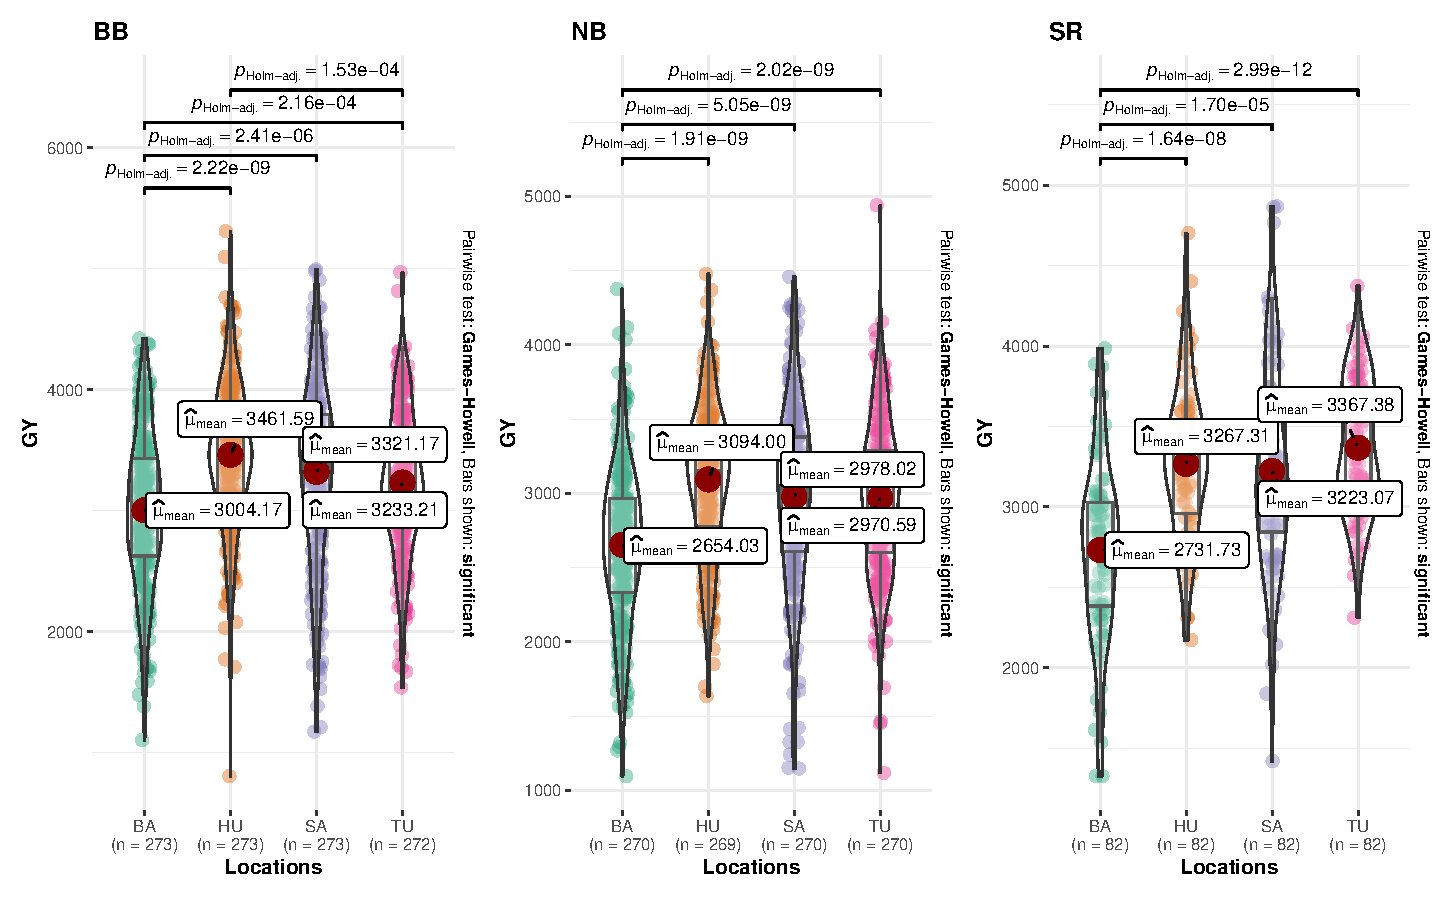
\includegraphics[width=1\linewidth]{figures/plot_ggstatsplot_met-1} 

}

\caption{Combination of box and violin plots along with jittered data points for between subjects comparisons by locations of grain yield (GY) for black (BB), Navy (NB) and Red (SR) beans. Pairwise Games-Howell test used. Comparisons showing only significant values. BA: Bay, HU: Huron, SA:Sanilac, TU: Tuscola.}\label{fig:plot_ggstatsplot_met}
\end{figure}

\begin{Shaded}
\begin{Highlighting}[]
\CommentTok{\#https://indrajeetpatil.github.io/ggstatsplot\_slides/slides/ggstatsplot\_presentation.html\#1}
\end{Highlighting}
\end{Shaded}

\begin{Shaded}
\begin{Highlighting}[]
\NormalTok{plotDM\_stats\_mkt\_loc}\OtherTok{\textless{}{-}} \FunctionTok{ggbetweenstats}\NormalTok{(}\AttributeTok{data=}\NormalTok{blues\_stage.I, }\AttributeTok{x=}\NormalTok{ loc, }\AttributeTok{y=}\NormalTok{yield, }\AttributeTok{type =} \StringTok{"parametric"}\NormalTok{,  }\AttributeTok{bf.message =}\NormalTok{ F, }\AttributeTok{results.subtitle =}\NormalTok{ F, }
                              \AttributeTok{ylab=} \StringTok{"GY"}\NormalTok{, }\AttributeTok{xlab =} \StringTok{"Locations"}\NormalTok{,}
                              \AttributeTok{plot.type =} \StringTok{"boxviolin"}
\NormalTok{                              ) }

\FunctionTok{print}\NormalTok{(plotDM\_stats\_mkt\_loc)}
\end{Highlighting}
\end{Shaded}

\begin{figure}[H]

{\centering 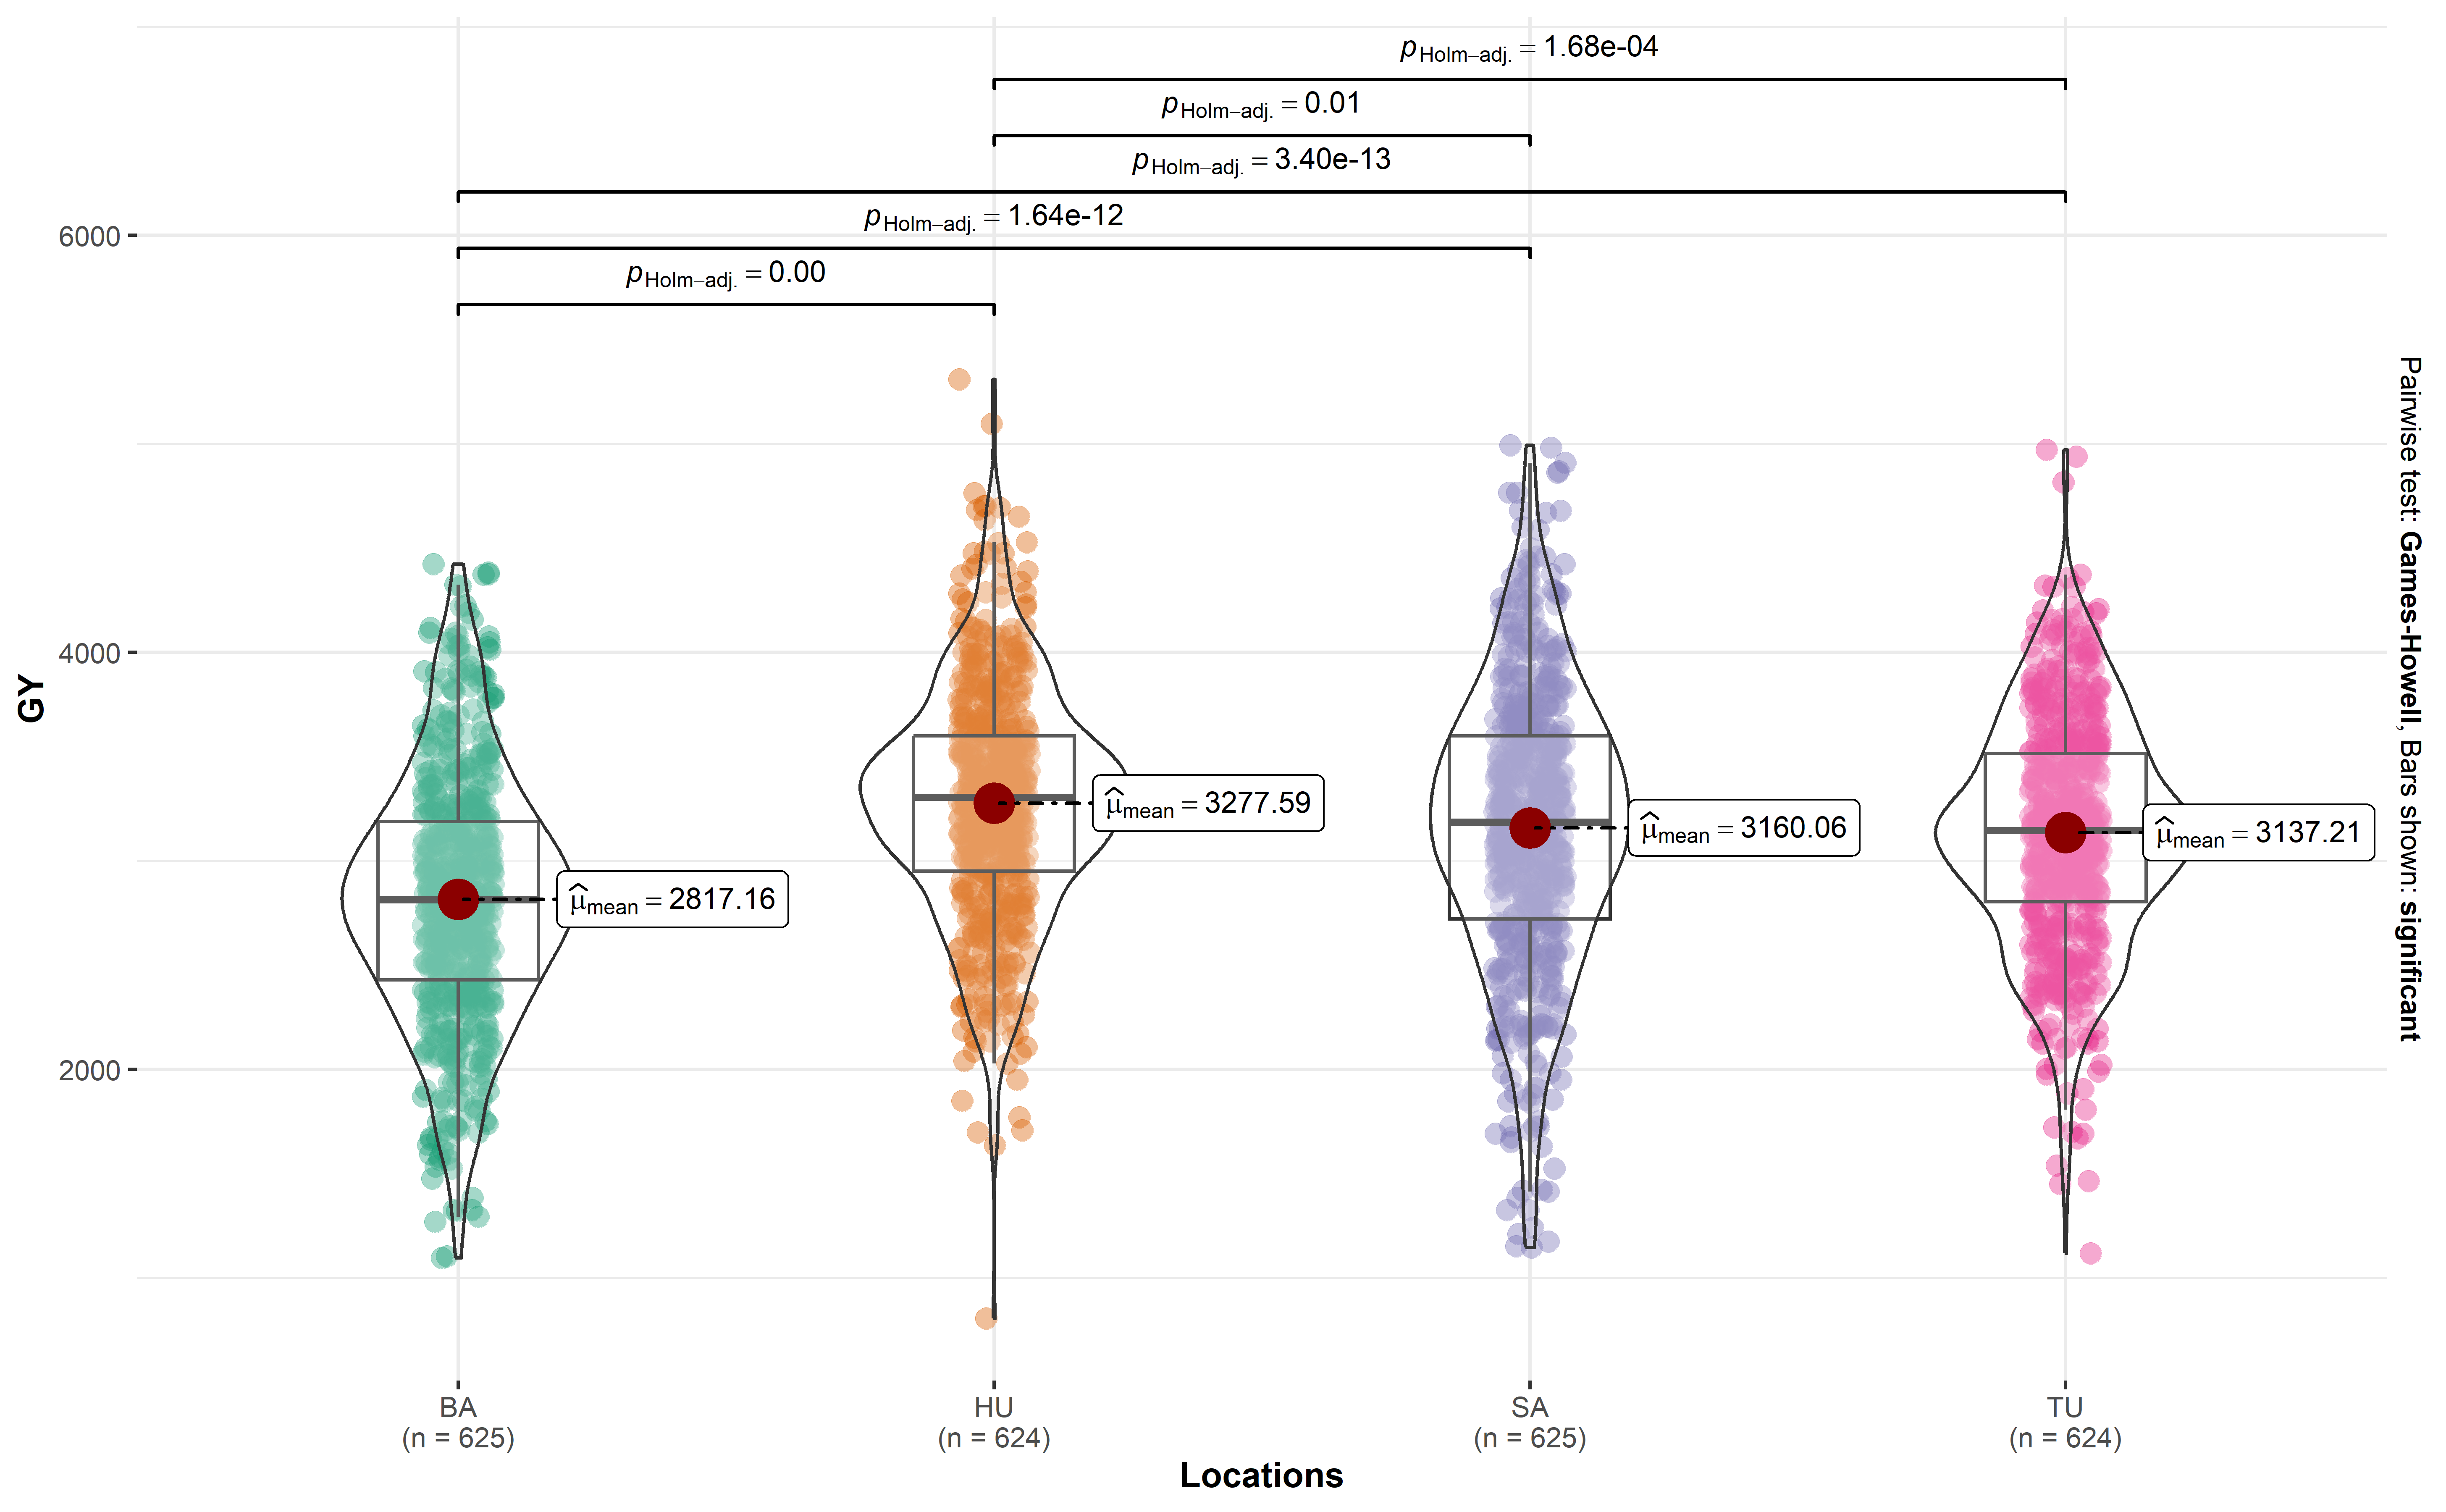
\includegraphics[width=1\linewidth]{figures/plot_ggstatsplot_met2-1} 

}

\caption{Combination of box and violin plots along with jittered data points for between subjects comparisons by locations of grain yield (GY) for the combined analysis (CombMKT) across all market classes. Pairwise Games-Howell test used. Comparisons showing only significant values. BA: Bay, HU: Huron, SA:Sanilac, TU: Tuscola.}\label{fig:plot_ggstatsplot_met2}
\end{figure}

\begin{Shaded}
\begin{Highlighting}[]
\CommentTok{\#https://indrajeetpatil.github.io/ggstatsplot\_slides/slides/ggstatsplot\_presentation.html\#1}
\end{Highlighting}
\end{Shaded}

\pagebreak

\hypertarget{phenotypic-variance-components}{%
\paragraph{Phenotypic variance
components}\label{phenotypic-variance-components}}

\begin{Shaded}
\begin{Highlighting}[]
\NormalTok{data\_beans\_var }\OtherTok{=} \FunctionTok{read.csv}\NormalTok{(}\StringTok{"data/VarStack.csv"}\NormalTok{,}\AttributeTok{h=}\NormalTok{T, }\AttributeTok{stringsAsFactors =}\NormalTok{ T)}
\NormalTok{data\_beans\_var}\SpecialCharTok{$}\NormalTok{trait }\OtherTok{\textless{}{-}} \FunctionTok{factor}\NormalTok{(data\_beans\_var}\SpecialCharTok{$}\NormalTok{trait, }\AttributeTok{levels=}\FunctionTok{c}\NormalTok{(}\StringTok{"GY1"}\NormalTok{, }\StringTok{"GY2"}\NormalTok{, }\StringTok{"DM"}\NormalTok{, }\StringTok{"PH"}\NormalTok{, }\StringTok{"LD"}\NormalTok{))}

\FunctionTok{ggplot}\NormalTok{(data\_beans\_var, }\FunctionTok{aes}\NormalTok{(}\AttributeTok{x =}\NormalTok{ trait, }\AttributeTok{y =}\NormalTok{ Freq, }\AttributeTok{fill =}\NormalTok{ Comp, }\AttributeTok{label =}\NormalTok{ Comp)) }\SpecialCharTok{+}
  \FunctionTok{geom\_bar}\NormalTok{(}\AttributeTok{stat =} \StringTok{"identity"}\NormalTok{) }\SpecialCharTok{+}
  \CommentTok{\#geom\_text(size = 3, position = position\_stack(vjust = 0.5)) +}
  \FunctionTok{facet\_wrap}\NormalTok{(}\StringTok{"mkt"}\NormalTok{) }\SpecialCharTok{+}
  \FunctionTok{geom\_text}\NormalTok{(}\FunctionTok{aes}\NormalTok{(}\AttributeTok{label =} \FunctionTok{round}\NormalTok{(Freq, }\DecValTok{2}\NormalTok{), }\AttributeTok{x =}\NormalTok{ trait, }\AttributeTok{y =}\NormalTok{ Freq), }\AttributeTok{data =}\NormalTok{ data\_beans\_var,}\AttributeTok{size =} \DecValTok{5}\NormalTok{, }\AttributeTok{position =} \FunctionTok{position\_stack}\NormalTok{(}\AttributeTok{vjust =} \FloatTok{0.5}\NormalTok{),}\AttributeTok{fontface =} \StringTok{"bold"}\NormalTok{) }\SpecialCharTok{+}
  \FunctionTok{labs}\NormalTok{(}\AttributeTok{y =} \StringTok{"Proportion of phenotypic variance"}\NormalTok{, }\AttributeTok{fill =} \StringTok{""}\NormalTok{, }\AttributeTok{x =} \ConstantTok{NULL}\NormalTok{) }\SpecialCharTok{+}
  \FunctionTok{theme\_classic}\NormalTok{() }\SpecialCharTok{+}
  \CommentTok{\#theme(strip.background = element\_blank()) +}
  \FunctionTok{scale\_fill\_manual}\NormalTok{(}\AttributeTok{values=}\FunctionTok{c}\NormalTok{(}\StringTok{"\#CC6666"}\NormalTok{, }\StringTok{"\#9999CC"}\NormalTok{, }\StringTok{"\#66CC99"}\NormalTok{),}
                    \AttributeTok{labels =} \FunctionTok{c}\NormalTok{(}\StringTok{"Res"}\NormalTok{, }\StringTok{"G"}\NormalTok{, }\StringTok{"GxE"}\NormalTok{)) }\SpecialCharTok{+}
  \FunctionTok{theme}\NormalTok{(}\AttributeTok{legend.position =} \StringTok{"bottom"}\NormalTok{,}
        \AttributeTok{axis.text.x=}\FunctionTok{element\_text}\NormalTok{(}\AttributeTok{face=}\StringTok{"bold"}\NormalTok{, }\AttributeTok{size =} \DecValTok{12}\NormalTok{),}
        \AttributeTok{axis.text.y=}\FunctionTok{element\_blank}\NormalTok{(),}
        \AttributeTok{axis.ticks.y =} \FunctionTok{element\_blank}\NormalTok{(),}
        \AttributeTok{axis.title.y=}\FunctionTok{element\_text}\NormalTok{(}\AttributeTok{face=}\StringTok{"bold"}\NormalTok{, }\AttributeTok{size =} \DecValTok{14}\NormalTok{) ,}
        \AttributeTok{legend.text =} \FunctionTok{element\_text}\NormalTok{(}\AttributeTok{size =} \DecValTok{12}\NormalTok{, }\AttributeTok{face=}\StringTok{"bold"}\NormalTok{), ) }\SpecialCharTok{+}
  \FunctionTok{scale\_y\_continuous}\NormalTok{(}\AttributeTok{expand =} \FunctionTok{expansion}\NormalTok{(}\AttributeTok{mult =} \FunctionTok{c}\NormalTok{(}\DecValTok{0}\NormalTok{, }\FloatTok{0.01}\NormalTok{)))}
\end{Highlighting}
\end{Shaded}

\begin{figure}[H]

{\centering 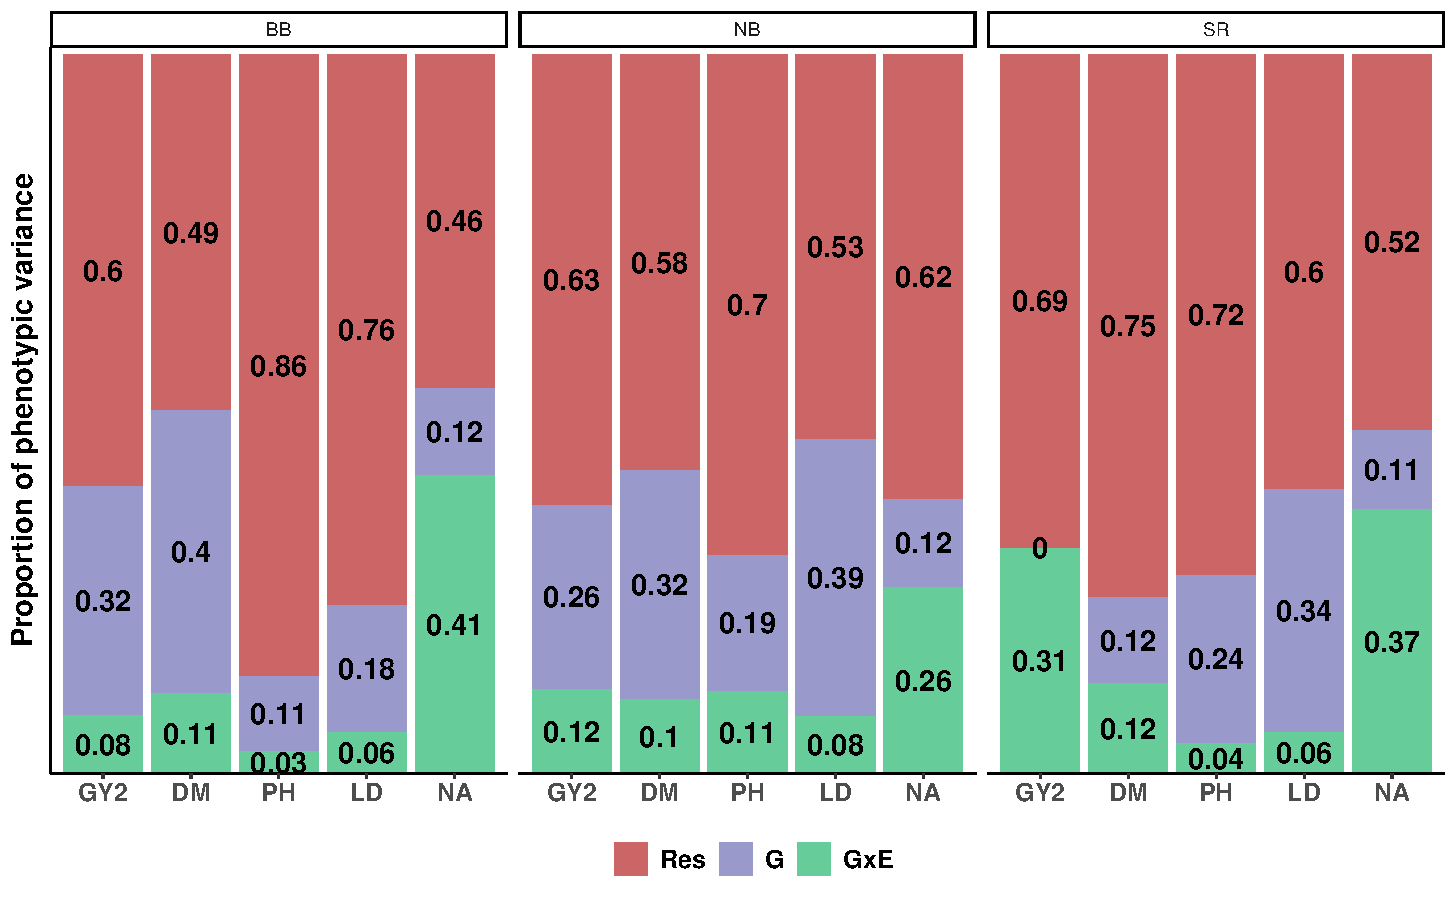
\includegraphics[width=1\linewidth]{figures/coincidence geno1-1} 

}

\caption{Proportion of the phenotypic variance for three dry beans traits evaluated across three locations. GY1, grain yield from 2017 to 2022; GY2, grain yield only in 2021; DM, days to maturity; PH, plant height; LD, lodging.}\label{fig:coincidence geno1}
\end{figure}

\pagebreak

\hypertarget{genotyping-performance}{%
\paragraph{Genotyping performance}\label{genotyping-performance}}

\begin{Shaded}
\begin{Highlighting}[]
\NormalTok{blues\_stage.I\_BB\_ge}\OtherTok{\textless{}{-}} \FunctionTok{na.omit}\NormalTok{(blues\_stage.I\_BB)}
\NormalTok{stab\_bb }\OtherTok{\textless{}{-}} \FunctionTok{ge\_plot}\NormalTok{(blues\_stage.I\_BB\_ge, }\AttributeTok{type =} \DecValTok{1}\NormalTok{,}
        \AttributeTok{env =}\NormalTok{ loc,}
        \AttributeTok{gen =}\NormalTok{ name,}
        \AttributeTok{resp =}\NormalTok{ yield) }\SpecialCharTok{+} \FunctionTok{xlab}\NormalTok{(}\StringTok{""}\NormalTok{) }\SpecialCharTok{+} \FunctionTok{ylab}\NormalTok{(}\StringTok{"Genotypes"}\NormalTok{) }\SpecialCharTok{+}
\FunctionTok{theme}\NormalTok{(}\AttributeTok{axis.text.x =} \FunctionTok{element\_text}\NormalTok{(}\AttributeTok{size =} \DecValTok{8}\NormalTok{, }\AttributeTok{angle =} \DecValTok{90}\NormalTok{, }\AttributeTok{vjust =} \FloatTok{0.5}\NormalTok{, }\AttributeTok{hjust =} \DecValTok{1}\NormalTok{),}
      \AttributeTok{axis.text.y =} \FunctionTok{element\_text}\NormalTok{(}\AttributeTok{size =} \DecValTok{7}\NormalTok{, }\AttributeTok{angle =} \DecValTok{0}\NormalTok{, }\AttributeTok{vjust =} \FloatTok{0.5}\NormalTok{, }\AttributeTok{hjust =} \DecValTok{1}\NormalTok{),}
      \AttributeTok{legend.position =}\StringTok{"none"}\NormalTok{, }\AttributeTok{plot.title=}\FunctionTok{element\_text}\NormalTok{(}\AttributeTok{hjust=}\FloatTok{0.5}\NormalTok{)) }\SpecialCharTok{+}
  \FunctionTok{labs}\NormalTok{(}\AttributeTok{title =} \StringTok{"BB"}\NormalTok{)}
\CommentTok{\#print (stab\_bb)}


\NormalTok{blues\_stage.I\_NB\_ge}\OtherTok{\textless{}{-}} \FunctionTok{na.omit}\NormalTok{(blues\_stage.I\_NB)}
\NormalTok{stab\_nb }\OtherTok{\textless{}{-}} \FunctionTok{ge\_plot}\NormalTok{(blues\_stage.I\_NB\_ge, }\AttributeTok{type =} \DecValTok{1}\NormalTok{,}
        \AttributeTok{env =}\NormalTok{ loc,}
        \AttributeTok{gen =}\NormalTok{ name,}
        \AttributeTok{resp =}\NormalTok{ yield) }\SpecialCharTok{+} \FunctionTok{xlab}\NormalTok{(}\StringTok{"Locations"}\NormalTok{) }\SpecialCharTok{+} \FunctionTok{ylab}\NormalTok{(}\StringTok{""}\NormalTok{) }\SpecialCharTok{+}
\FunctionTok{theme}\NormalTok{(}\AttributeTok{axis.text.x =} \FunctionTok{element\_text}\NormalTok{(}\AttributeTok{size =} \DecValTok{8}\NormalTok{, }\AttributeTok{angle =} \DecValTok{90}\NormalTok{, }\AttributeTok{vjust =} \FloatTok{0.5}\NormalTok{, }\AttributeTok{hjust =} \DecValTok{1}\NormalTok{),}
      \AttributeTok{axis.text.y =} \FunctionTok{element\_text}\NormalTok{(}\AttributeTok{size =} \DecValTok{7}\NormalTok{, }\AttributeTok{angle =} \DecValTok{0}\NormalTok{, }\AttributeTok{vjust =} \FloatTok{0.5}\NormalTok{, }\AttributeTok{hjust =} \DecValTok{1}\NormalTok{),}
      \AttributeTok{legend.position =}\StringTok{"none"}\NormalTok{, }\AttributeTok{plot.title=}\FunctionTok{element\_text}\NormalTok{(}\AttributeTok{hjust=}\FloatTok{0.5}\NormalTok{)) }\SpecialCharTok{+}
  \FunctionTok{labs}\NormalTok{(}\AttributeTok{title =} \StringTok{"NB"}\NormalTok{)}
\CommentTok{\#print (stab\_nb)}

\NormalTok{blues\_stage.I\_SR\_ge}\OtherTok{\textless{}{-}} \FunctionTok{na.omit}\NormalTok{(blues\_stage.I\_SR)}
\NormalTok{stab\_sr }\OtherTok{\textless{}{-}} \FunctionTok{ge\_plot}\NormalTok{(blues\_stage.I\_SR\_ge, }\AttributeTok{type =} \DecValTok{1}\NormalTok{,}
        \AttributeTok{env =}\NormalTok{ loc,}
        \AttributeTok{gen =}\NormalTok{ name,}
        \AttributeTok{resp =}\NormalTok{ yield) }\SpecialCharTok{+} \FunctionTok{xlab}\NormalTok{(}\StringTok{""}\NormalTok{) }\SpecialCharTok{+} \FunctionTok{ylab}\NormalTok{(}\StringTok{""}\NormalTok{) }\SpecialCharTok{+}
\FunctionTok{theme}\NormalTok{(}\AttributeTok{axis.text.x =} \FunctionTok{element\_text}\NormalTok{(}\AttributeTok{size =} \DecValTok{8}\NormalTok{, }\AttributeTok{angle =} \DecValTok{90}\NormalTok{, }\AttributeTok{vjust =} \FloatTok{0.5}\NormalTok{, }\AttributeTok{hjust =} \DecValTok{1}\NormalTok{),}
      \AttributeTok{axis.text.y =} \FunctionTok{element\_text}\NormalTok{(}\AttributeTok{size =} \DecValTok{7}\NormalTok{, }\AttributeTok{angle =} \DecValTok{0}\NormalTok{, }\AttributeTok{vjust =} \FloatTok{0.5}\NormalTok{, }\AttributeTok{hjust =} \DecValTok{1}\NormalTok{),}
      \AttributeTok{legend.position =}\StringTok{"right"}\NormalTok{, }
      \AttributeTok{plot.title=}\FunctionTok{element\_text}\NormalTok{(}\AttributeTok{hjust=}\FloatTok{0.5}\NormalTok{)) }\SpecialCharTok{+}
  \FunctionTok{labs}\NormalTok{(}\AttributeTok{fill=}\StringTok{"GY(Kg/ha)"}\NormalTok{, }\AttributeTok{title =} \StringTok{"SR"}\NormalTok{)}
\CommentTok{\#print (stab\_sr)}

\FunctionTok{print}\NormalTok{(}\FunctionTok{arrange\_ggplot}\NormalTok{(stab\_bb, stab\_nb,stab\_sr))}
\end{Highlighting}
\end{Shaded}

\begin{figure}[H]

{\centering 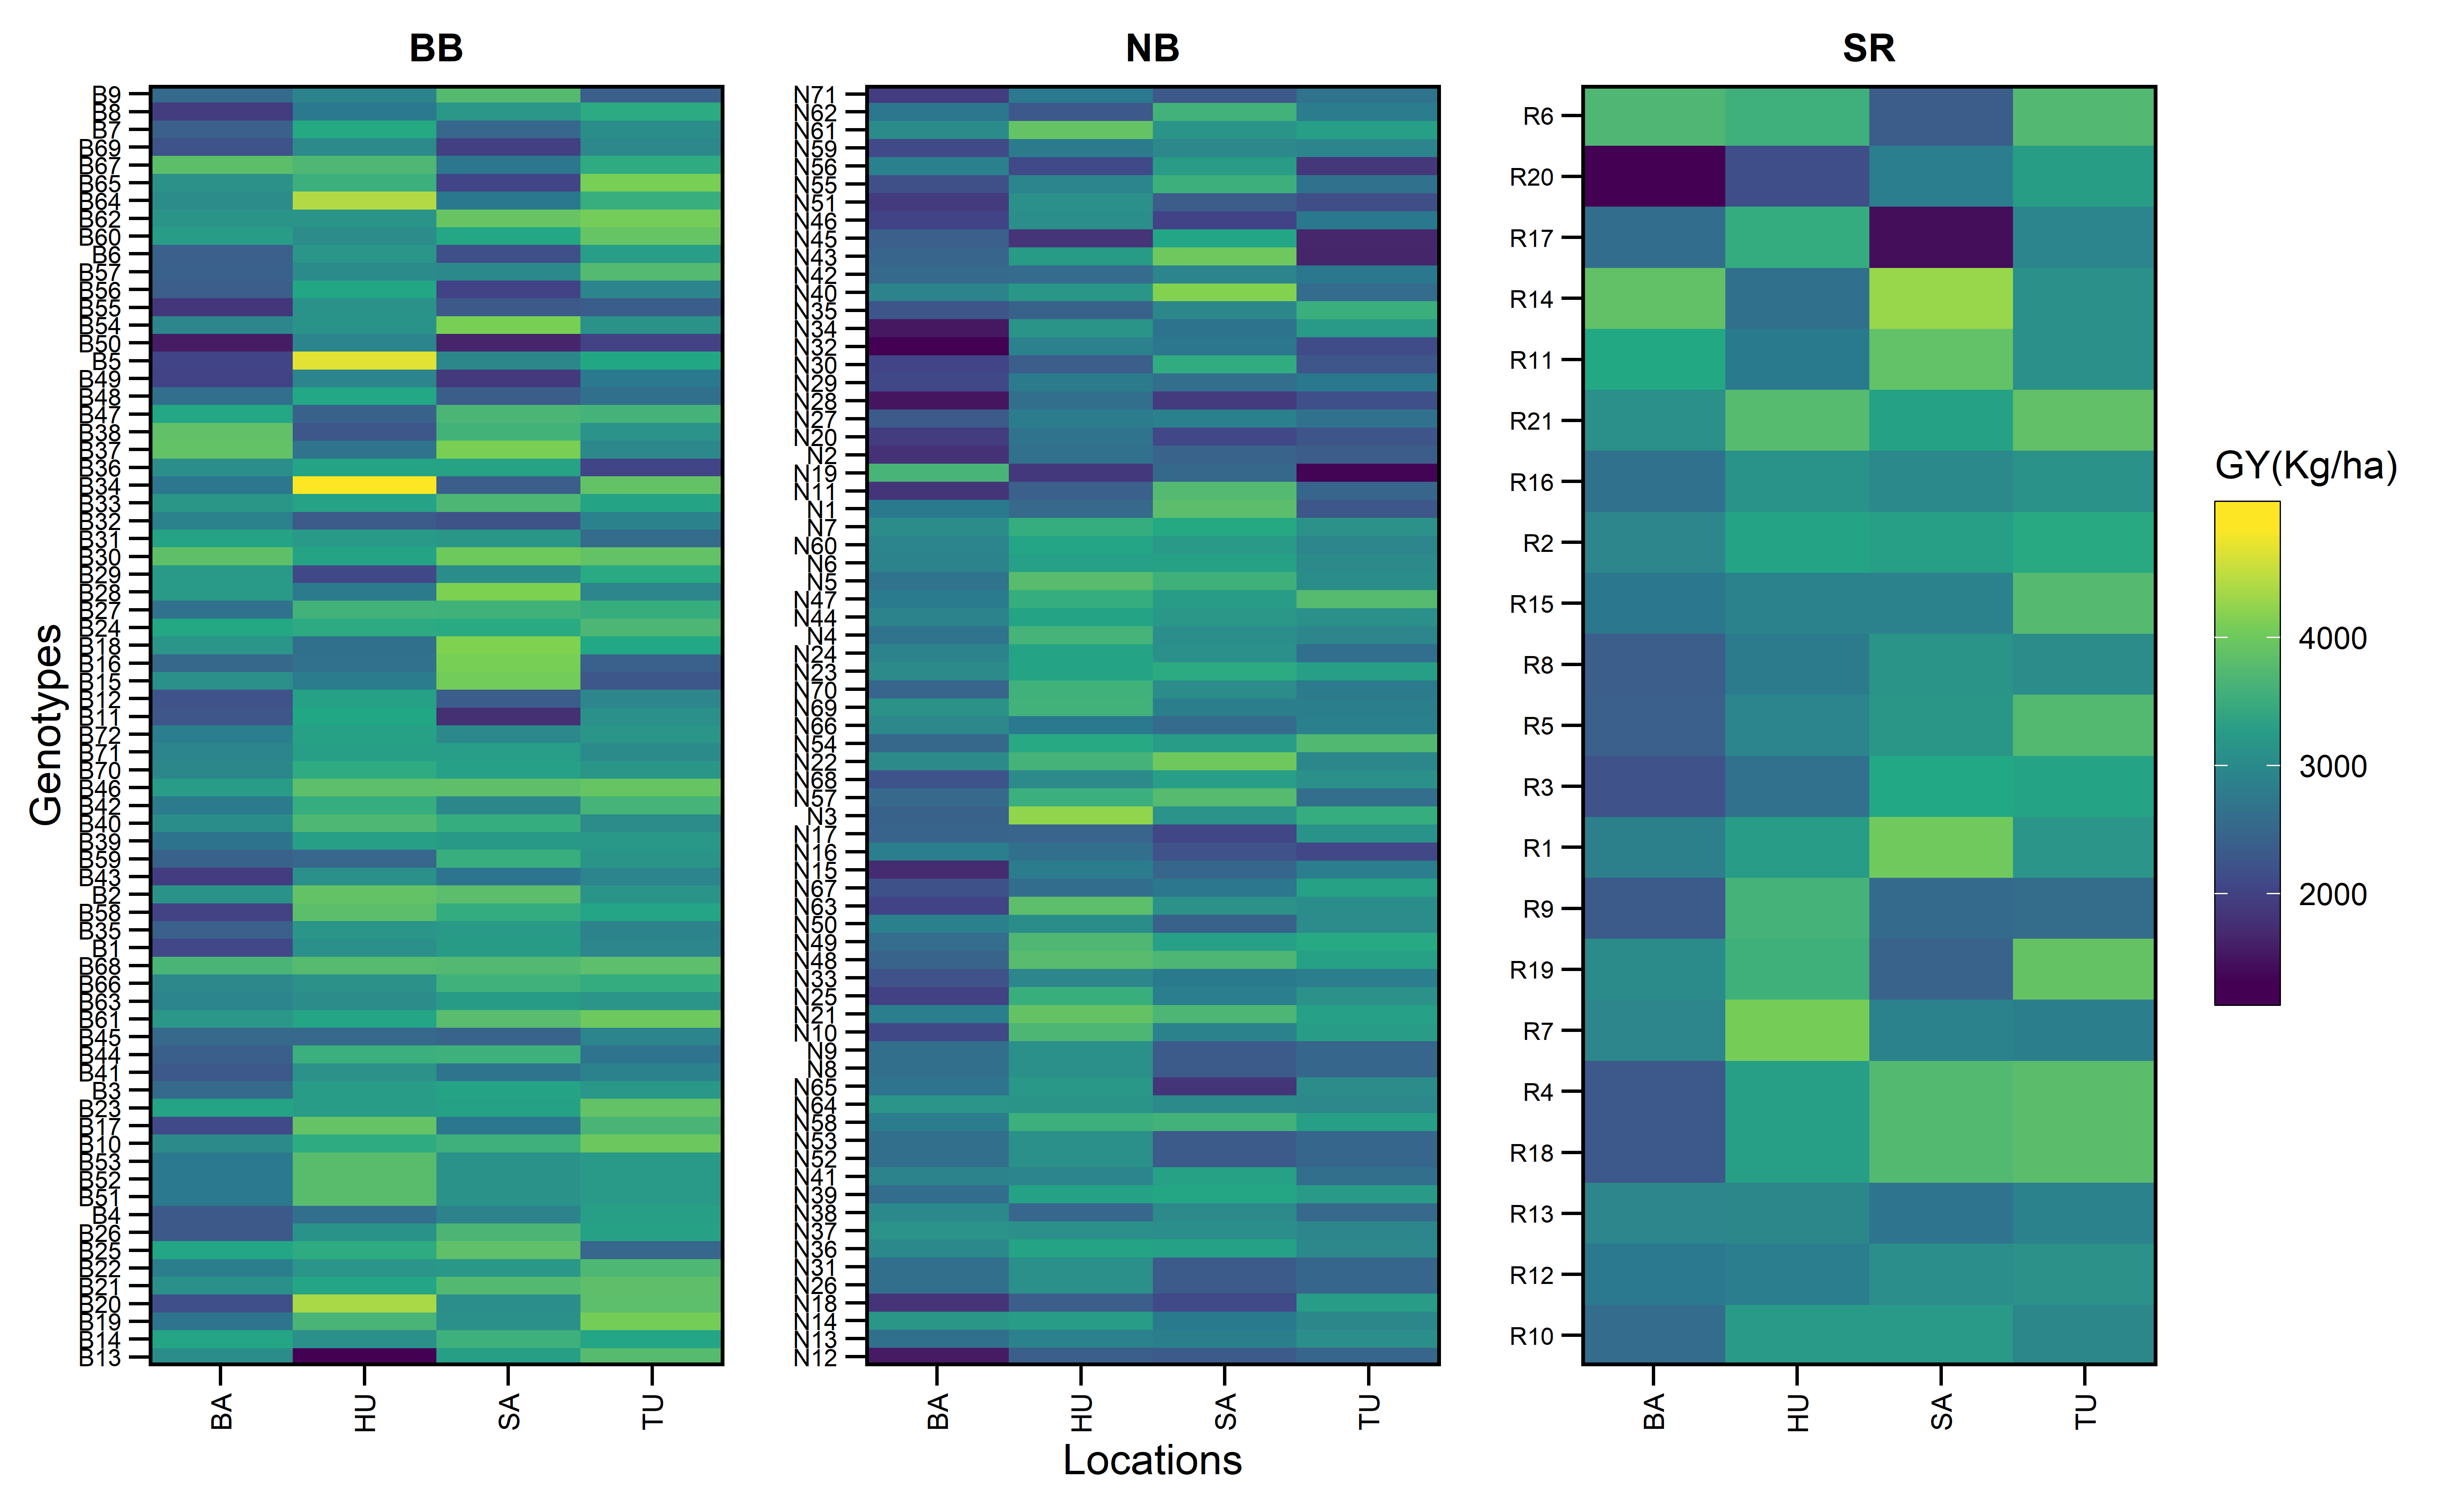
\includegraphics{figures/MET metan-1} 

}

\caption{Genotype’s performance across the environments for Black (BB), Navy (NB), and Small Red (SR) beans using the estimated means (BLUEs) from the 1-stage mixed model analysis. }\label{fig:MET metan}
\end{figure}

\begin{Shaded}
\begin{Highlighting}[]
\NormalTok{stab\_allMKT }\OtherTok{\textless{}{-}} \FunctionTok{ge\_plot}\NormalTok{(blues\_stage.I, }\AttributeTok{type =} \DecValTok{1}\NormalTok{,}
        \AttributeTok{env =}\NormalTok{ loc,}
        \AttributeTok{gen =}\NormalTok{ name,}
        \AttributeTok{resp =}\NormalTok{ yield) }\SpecialCharTok{+} \FunctionTok{xlab}\NormalTok{(}\StringTok{""}\NormalTok{) }\SpecialCharTok{+} \FunctionTok{ylab}\NormalTok{(}\StringTok{"Genotypes"}\NormalTok{) }\SpecialCharTok{+}
\FunctionTok{theme}\NormalTok{(}\AttributeTok{axis.text.x =} \FunctionTok{element\_text}\NormalTok{(}\AttributeTok{size =} \DecValTok{8}\NormalTok{, }\AttributeTok{angle =} \DecValTok{90}\NormalTok{, }\AttributeTok{vjust =} \FloatTok{0.5}\NormalTok{, }\AttributeTok{hjust =} \DecValTok{1}\NormalTok{),}
      \AttributeTok{axis.text.y =} \FunctionTok{element\_text}\NormalTok{(}\AttributeTok{size =} \DecValTok{7}\NormalTok{, }\AttributeTok{angle =} \DecValTok{0}\NormalTok{, }\AttributeTok{vjust =} \FloatTok{0.5}\NormalTok{, }\AttributeTok{hjust =} \DecValTok{1}\NormalTok{),}
      \AttributeTok{legend.position =}\StringTok{"none"}\NormalTok{, }\AttributeTok{plot.title=}\FunctionTok{element\_text}\NormalTok{(}\AttributeTok{hjust=}\FloatTok{0.5}\NormalTok{)) }\SpecialCharTok{+}
  \FunctionTok{labs}\NormalTok{(}\AttributeTok{title =} \StringTok{"Comb\_MKT"}\NormalTok{)}

\FunctionTok{print}\NormalTok{(stab\_allMKT)}
\end{Highlighting}
\end{Shaded}

\begin{figure}[H]

{\centering 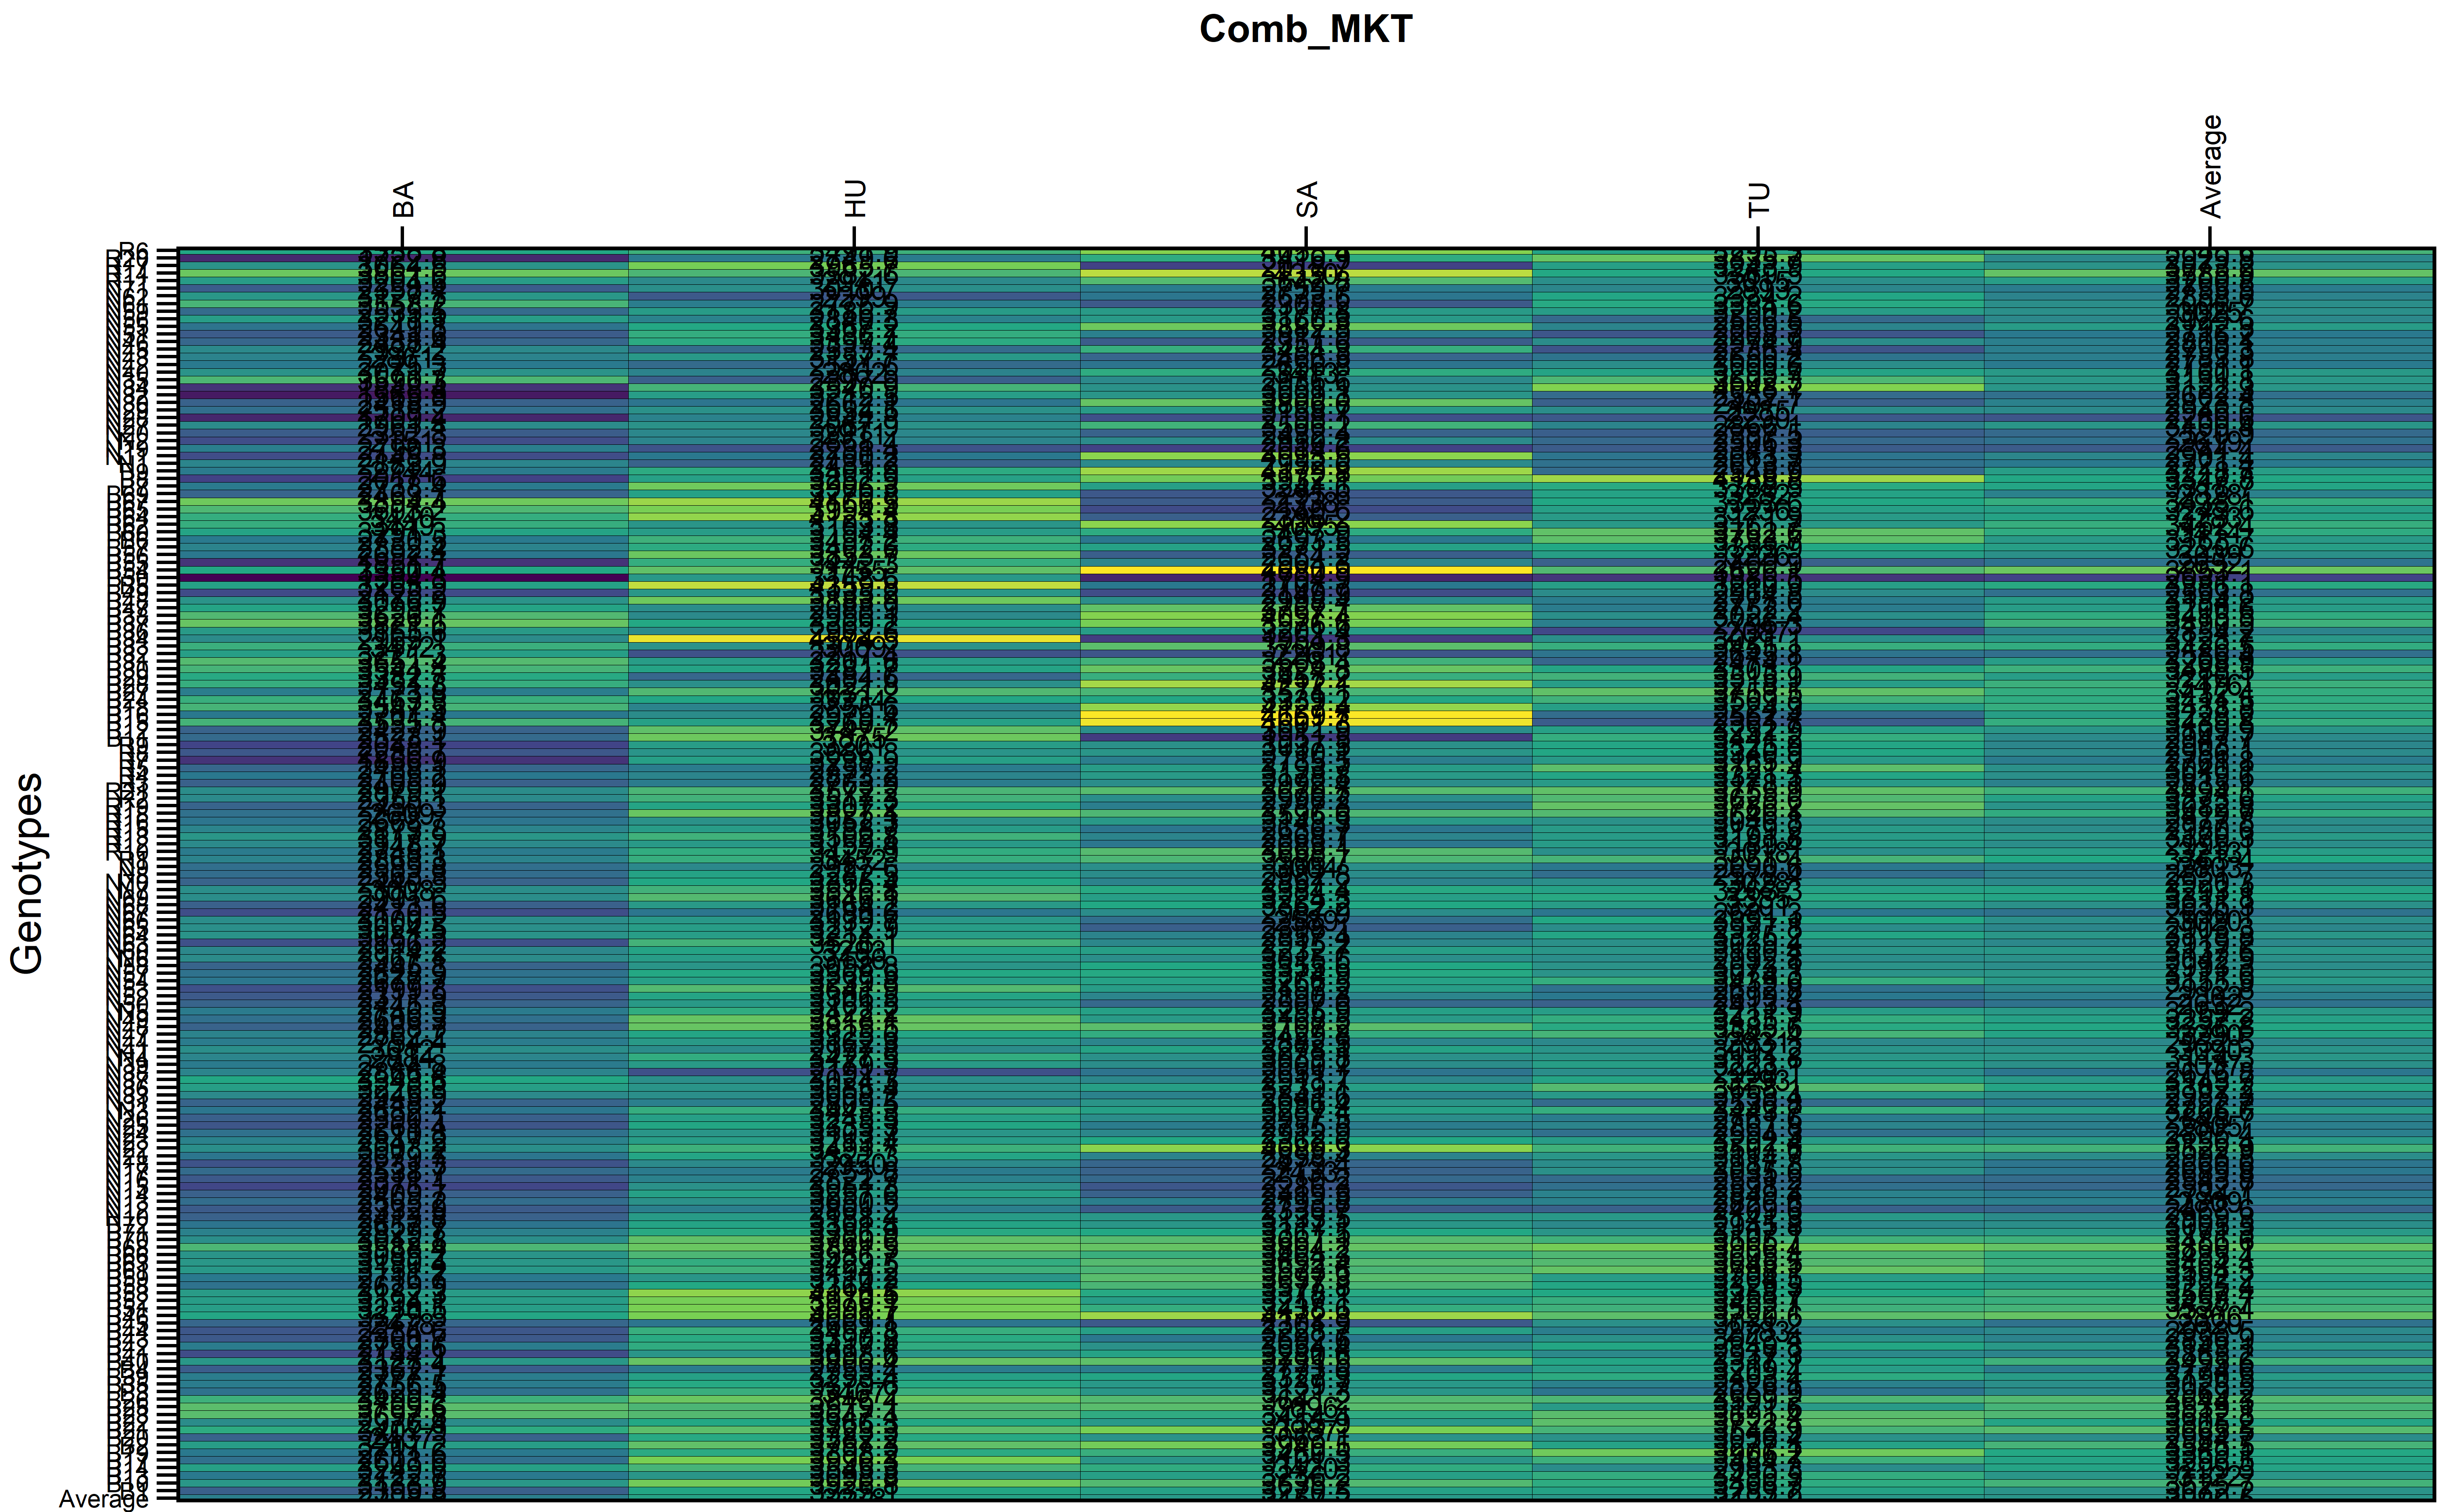
\includegraphics{figures/MET metan all mkt-1} 

}

\caption{Genotype’s performance across the environments for all beans maket classes combined (combMKT)  using the estimated means (BLUEs) from the 1-stage mixed model analysis. }\label{fig:MET metan all mkt}
\end{figure}

\pagebreak

\hypertarget{descriptive-met}{%
\subsection{Descriptive MET}\label{descriptive-met}}

\begin{itemize}
\tightlist
\item
  Genetic correlations across environment using the Unstructured (US)
  variance-covariance structure.
\end{itemize}

This mixed model will be used only for genotype x environment
correlations in order to investigate the GEI correlations.

Combined analysis across all market classes (Comb\_MKT)

\begin{Shaded}
\begin{Highlighting}[]
\NormalTok{mod.us.all }\OtherTok{\textless{}{-}} \FunctionTok{asreml}\NormalTok{(}\AttributeTok{fixed =}\NormalTok{ yield }\SpecialCharTok{\textasciitilde{}}\NormalTok{ loc }\SpecialCharTok{+}\NormalTok{ loc}\SpecialCharTok{:}\NormalTok{rep ,}
                      \AttributeTok{random =} \SpecialCharTok{\textasciitilde{}}\NormalTok{ name}\SpecialCharTok{:}\FunctionTok{us}\NormalTok{(loc) ,}
                      \AttributeTok{data =}\NormalTok{ blues\_stage.I,}
                      \AttributeTok{predict =} \FunctionTok{predict.asreml}\NormalTok{(}\AttributeTok{classify =} \StringTok{"name"}\NormalTok{),}
                      \AttributeTok{trace =}\NormalTok{ F,}
                      \AttributeTok{maxit =} \DecValTok{500}\NormalTok{)}
\CommentTok{\#print(wald(mod.us.bb))}
\CommentTok{\#print(summary.asreml(mod.us.bb)$varcomp)}
\NormalTok{f}\OtherTok{=}\FunctionTok{summary}\NormalTok{(mod.us.all)}\SpecialCharTok{$}\NormalTok{varcomp[}\DecValTok{1}\SpecialCharTok{:}\DecValTok{10}\NormalTok{,}\DecValTok{1}\NormalTok{]}
\NormalTok{z}\OtherTok{=}\FunctionTok{matrix}\NormalTok{(}\DecValTok{0}\NormalTok{, }\DecValTok{4}\NormalTok{,}\DecValTok{4}\NormalTok{)}
\NormalTok{z[}\FunctionTok{upper.tri}\NormalTok{(z)}\SpecialCharTok{|} \FunctionTok{row}\NormalTok{(z)}\SpecialCharTok{==}\FunctionTok{col}\NormalTok{(z)] }\OtherTok{\textless{}{-}}\NormalTok{ f}
\NormalTok{corf}\OtherTok{=}\NormalTok{z}\SpecialCharTok{/}\FunctionTok{sqrt}\NormalTok{(}\FunctionTok{diag}\NormalTok{(z)}\SpecialCharTok{\%*\%}\FunctionTok{t}\NormalTok{(}\FunctionTok{diag}\NormalTok{(z)))}
\CommentTok{\#corf}
\FunctionTok{rownames}\NormalTok{(corf)}\OtherTok{=}\FunctionTok{c}\NormalTok{(}
\StringTok{"BA"}\NormalTok{,}
\StringTok{"HU"}\NormalTok{,}
\StringTok{"SA"}\NormalTok{,}
\StringTok{"TU"}\NormalTok{)}
\FunctionTok{colnames}\NormalTok{(corf)}\OtherTok{=}\FunctionTok{rownames}\NormalTok{(corf)}
\NormalTok{plotAll}\OtherTok{\textless{}{-}} \FunctionTok{ggcorrplot}\NormalTok{(corf, }\AttributeTok{colors =} \FunctionTok{c}\NormalTok{(}\StringTok{"\#6D9EC1"}\NormalTok{, }\StringTok{"white"}\NormalTok{, }\StringTok{"\#E46726"}\NormalTok{),}
\AttributeTok{title =} \StringTok{" Comb\_MKT"}\NormalTok{,}
\AttributeTok{show.legend =}\NormalTok{ F,}
\AttributeTok{legend.title =} \StringTok{"rgg"}\NormalTok{ ,}\AttributeTok{lab\_size=}\DecValTok{5}\NormalTok{,}\AttributeTok{tl.srt =} \DecValTok{90}\NormalTok{,}\AttributeTok{type =} \FunctionTok{c}\NormalTok{(}\StringTok{"upper"}\NormalTok{), }\AttributeTok{lab =}\NormalTok{ T,}\AttributeTok{digits =} \DecValTok{4}\NormalTok{,}
\AttributeTok{outline.color =} \StringTok{"white"}\NormalTok{,}\AttributeTok{pch.col =} \StringTok{"white"}\NormalTok{, }\AttributeTok{tl.col =} \StringTok{"blue"}\NormalTok{,}\AttributeTok{show.diag =} \ConstantTok{FALSE}\NormalTok{)}
\FunctionTok{print}\NormalTok{(plotAll)}
\end{Highlighting}
\end{Shaded}

\begin{center}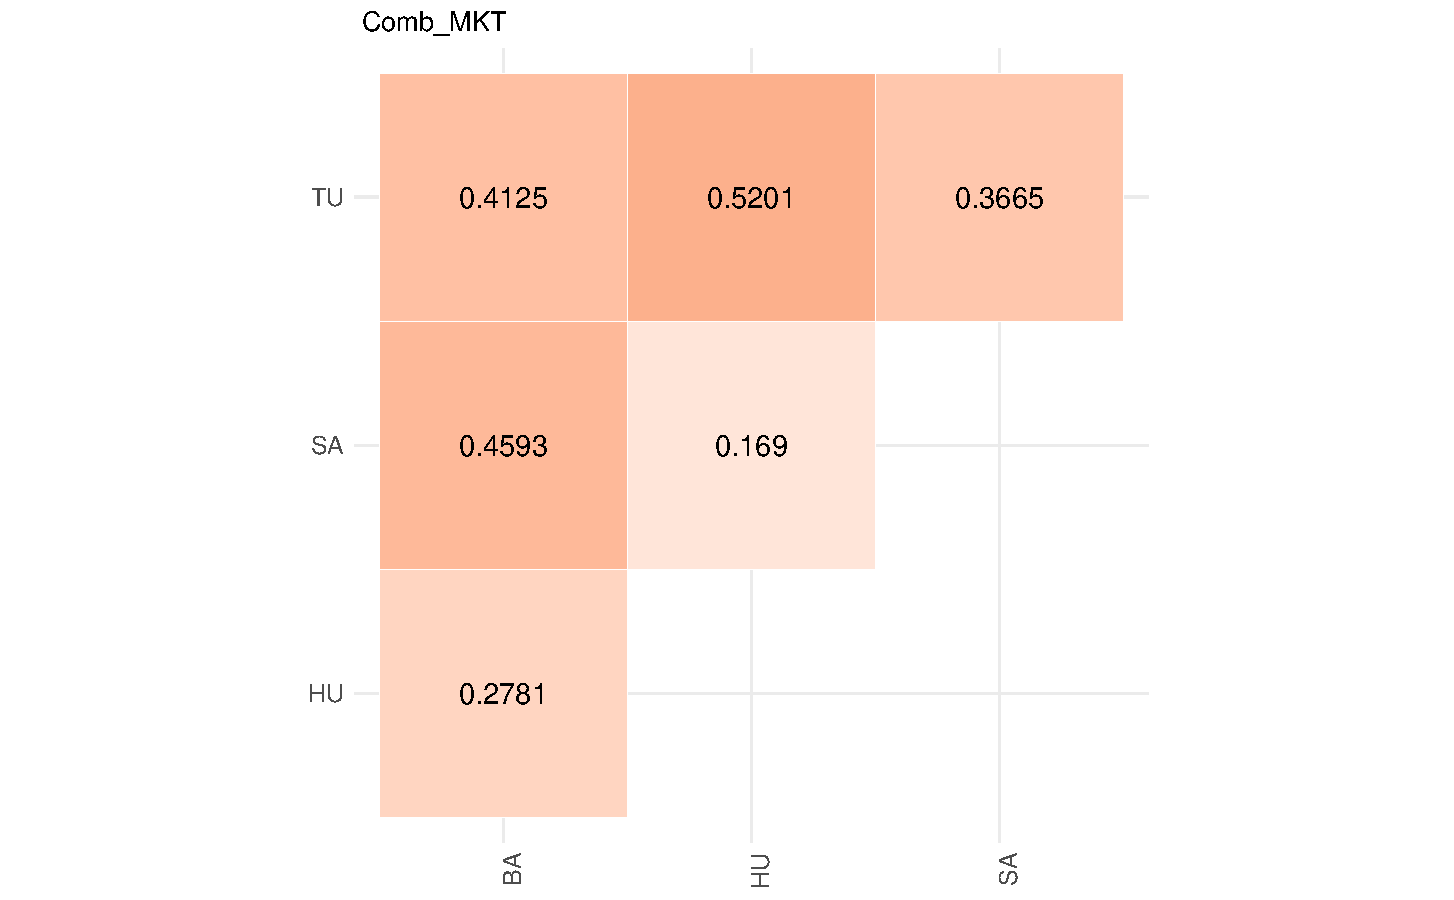
\includegraphics{figures/unnamed-chunk-158-1} \end{center}

\begin{Shaded}
\begin{Highlighting}[]
\NormalTok{mod.us.bb }\OtherTok{\textless{}{-}} \FunctionTok{asreml}\NormalTok{(}\AttributeTok{fixed =}\NormalTok{ yield }\SpecialCharTok{\textasciitilde{}}\NormalTok{  loc }\SpecialCharTok{+}\NormalTok{ loc}\SpecialCharTok{:}\NormalTok{rep ,}
                        \AttributeTok{random      =} \SpecialCharTok{\textasciitilde{}}\NormalTok{ name}\SpecialCharTok{:}\FunctionTok{us}\NormalTok{(loc) ,}
                        \AttributeTok{data        =}\NormalTok{ blues\_stage.I\_BB,}
                        \AttributeTok{predict     =} \FunctionTok{predict.asreml}\NormalTok{(}\AttributeTok{classify =} \StringTok{"name"}\NormalTok{),}
                        \AttributeTok{trace       =}\NormalTok{ F,}
                        \AttributeTok{maxit       =} \DecValTok{500}\NormalTok{)}

\CommentTok{\#print(wald(mod.us.bb))}
\CommentTok{\#print(summary.asreml(mod.us.bb)$varcomp)}

\NormalTok{f}\OtherTok{=}\FunctionTok{summary}\NormalTok{(mod.us.bb)}\SpecialCharTok{$}\NormalTok{varcomp[}\DecValTok{1}\SpecialCharTok{:}\DecValTok{10}\NormalTok{,}\DecValTok{1}\NormalTok{]}
\NormalTok{z}\OtherTok{=}\FunctionTok{matrix}\NormalTok{(}\DecValTok{0}\NormalTok{, }\DecValTok{4}\NormalTok{,}\DecValTok{4}\NormalTok{)}
\NormalTok{z[}\FunctionTok{upper.tri}\NormalTok{(z)}\SpecialCharTok{|} \FunctionTok{row}\NormalTok{(z)}\SpecialCharTok{==}\FunctionTok{col}\NormalTok{(z)] }\OtherTok{\textless{}{-}}\NormalTok{ f}
\NormalTok{corf}\OtherTok{=}\NormalTok{z}\SpecialCharTok{/}\FunctionTok{sqrt}\NormalTok{(}\FunctionTok{diag}\NormalTok{(z)}\SpecialCharTok{\%*\%}\FunctionTok{t}\NormalTok{(}\FunctionTok{diag}\NormalTok{(z)))}
\CommentTok{\#corf}

\FunctionTok{rownames}\NormalTok{(corf)}\OtherTok{=}\FunctionTok{c}\NormalTok{(}
\StringTok{"BA"}\NormalTok{,}
\StringTok{"HU"}\NormalTok{,}
\StringTok{"SA"}\NormalTok{,}
\StringTok{"TU"}\NormalTok{)}

\FunctionTok{colnames}\NormalTok{(corf)}\OtherTok{=}\FunctionTok{rownames}\NormalTok{(corf)}

\NormalTok{plotBB}\OtherTok{\textless{}{-}} \FunctionTok{ggcorrplot}\NormalTok{(corf, }\AttributeTok{colors =} \FunctionTok{c}\NormalTok{(}\StringTok{"\#6D9EC1"}\NormalTok{, }\StringTok{"white"}\NormalTok{, }\StringTok{"\#E46726"}\NormalTok{),  }
           \AttributeTok{title =} \StringTok{"                   Black Beans"}\NormalTok{,}
           \AttributeTok{show.legend =}\NormalTok{ F,}
\AttributeTok{legend.title =} \StringTok{"rgg"}\NormalTok{ ,}\AttributeTok{lab\_size=}\DecValTok{5}\NormalTok{,}\AttributeTok{tl.srt =} \DecValTok{90}\NormalTok{,}\AttributeTok{type =} \FunctionTok{c}\NormalTok{(}\StringTok{"upper"}\NormalTok{), }\AttributeTok{lab =}\NormalTok{ T,}\AttributeTok{digits =} \DecValTok{4}\NormalTok{,}
\AttributeTok{outline.color =} \StringTok{"white"}\NormalTok{,}\AttributeTok{pch.col =} \StringTok{"white"}\NormalTok{, }\AttributeTok{tl.col =} \StringTok{"blue"}\NormalTok{,}\AttributeTok{show.diag =} \ConstantTok{FALSE}\NormalTok{)}
\DocumentationTok{\#\# genetic correlation: manual estimation}
\CommentTok{\# corr.loc\_BA\_HU\textless{}{-}summary(mod.us.bb)$varcomp[2,1] /}
\CommentTok{\#   sqrt(summary(mod.us.bb)$varcomp[1,1]*summary(mod.us.bb)$varcomp[3,1])}

\CommentTok{\# print(plotBB)}

\NormalTok{mod.us.nb }\OtherTok{\textless{}{-}} \FunctionTok{asreml}\NormalTok{(}\AttributeTok{fixed =}\NormalTok{ yield }\SpecialCharTok{\textasciitilde{}}\NormalTok{  loc }\SpecialCharTok{+}\NormalTok{ loc}\SpecialCharTok{:}\NormalTok{rep ,}
                        \AttributeTok{random      =} \SpecialCharTok{\textasciitilde{}}\NormalTok{ name}\SpecialCharTok{:}\FunctionTok{us}\NormalTok{(loc) ,}
                        \AttributeTok{data        =}\NormalTok{ blues\_stage.I\_NB,}
                        \AttributeTok{predict     =} \FunctionTok{predict.asreml}\NormalTok{(}\AttributeTok{classify =} \StringTok{"name"}\NormalTok{),}
                        \AttributeTok{trace       =}\NormalTok{ F,}
                        \AttributeTok{maxit       =} \DecValTok{500}\NormalTok{)}

\CommentTok{\#print(wald(mod.us.nb))}
\CommentTok{\#print(summary.asreml(mod.us.nb)$varcomp)}

\NormalTok{f}\OtherTok{=}\FunctionTok{summary}\NormalTok{(mod.us.nb)}\SpecialCharTok{$}\NormalTok{varcomp[}\DecValTok{1}\SpecialCharTok{:}\DecValTok{10}\NormalTok{,}\DecValTok{1}\NormalTok{]}
\NormalTok{z}\OtherTok{=}\FunctionTok{matrix}\NormalTok{(}\DecValTok{0}\NormalTok{, }\DecValTok{4}\NormalTok{,}\DecValTok{4}\NormalTok{)}
\NormalTok{z[}\FunctionTok{upper.tri}\NormalTok{(z)}\SpecialCharTok{|} \FunctionTok{row}\NormalTok{(z)}\SpecialCharTok{==}\FunctionTok{col}\NormalTok{(z)] }\OtherTok{\textless{}{-}}\NormalTok{ f}
\NormalTok{corf}\OtherTok{=}\NormalTok{z}\SpecialCharTok{/}\FunctionTok{sqrt}\NormalTok{(}\FunctionTok{diag}\NormalTok{(z)}\SpecialCharTok{\%*\%}\FunctionTok{t}\NormalTok{(}\FunctionTok{diag}\NormalTok{(z)))}
\CommentTok{\#corf}

\FunctionTok{rownames}\NormalTok{(corf)}\OtherTok{=}\FunctionTok{c}\NormalTok{(}
\StringTok{"BA"}\NormalTok{,}
\StringTok{"HU"}\NormalTok{,}
\StringTok{"SA"}\NormalTok{,}
\StringTok{"TU"}\NormalTok{)}

\FunctionTok{colnames}\NormalTok{(corf)}\OtherTok{=}\FunctionTok{rownames}\NormalTok{(corf)}

\CommentTok{\#corf\textless{}{-} as\_tibble(corf,rownames=NA)}

\NormalTok{plotNB}\OtherTok{\textless{}{-}}\FunctionTok{ggcorrplot}\NormalTok{(corf, }\AttributeTok{colors =} \FunctionTok{c}\NormalTok{(}\StringTok{"\#6D9EC1"}\NormalTok{, }\StringTok{"white"}\NormalTok{, }\StringTok{"\#E46726"}\NormalTok{),  }
           \AttributeTok{title =} \StringTok{"                  Navy Beans"}\NormalTok{,}
           \AttributeTok{show.legend =}\NormalTok{ F,}
\AttributeTok{legend.title =} \StringTok{"r"}\NormalTok{ ,}\AttributeTok{lab\_size=}\DecValTok{5}\NormalTok{,}\AttributeTok{tl.srt =} \DecValTok{90}\NormalTok{,}\AttributeTok{type =} \FunctionTok{c}\NormalTok{(}\StringTok{"upper"}\NormalTok{), }\AttributeTok{lab =}\NormalTok{ T,}\AttributeTok{digits =} \DecValTok{4}\NormalTok{,}
\AttributeTok{outline.color =} \StringTok{"white"}\NormalTok{,}\AttributeTok{pch.col =} \StringTok{"white"}\NormalTok{, }\AttributeTok{tl.col =} \StringTok{"blue"}\NormalTok{,}\AttributeTok{show.diag =} \ConstantTok{FALSE}\NormalTok{)}
\DocumentationTok{\#\# genetic correlation: manual estimation}
\NormalTok{corr.loc}\OtherTok{\textless{}{-}}\FunctionTok{summary}\NormalTok{(mod.us.nb)}\SpecialCharTok{$}\NormalTok{varcomp[}\DecValTok{2}\NormalTok{,}\DecValTok{1}\NormalTok{] }\SpecialCharTok{/}
  \FunctionTok{sqrt}\NormalTok{(}\FunctionTok{summary}\NormalTok{(mod.us.nb)}\SpecialCharTok{$}\NormalTok{varcomp[}\DecValTok{1}\NormalTok{,}\DecValTok{1}\NormalTok{]}\SpecialCharTok{*}\FunctionTok{summary}\NormalTok{(mod.us.nb)}\SpecialCharTok{$}\NormalTok{varcomp[}\DecValTok{3}\NormalTok{,}\DecValTok{1}\NormalTok{])}
\CommentTok{\#print(plotNB)}

\NormalTok{mod.us.sr }\OtherTok{\textless{}{-}} \FunctionTok{asreml}\NormalTok{(}\AttributeTok{fixed =}\NormalTok{ yield }\SpecialCharTok{\textasciitilde{}}\NormalTok{  loc }\SpecialCharTok{+}\NormalTok{ loc}\SpecialCharTok{:}\NormalTok{rep ,}
                        \AttributeTok{random      =} \SpecialCharTok{\textasciitilde{}}\NormalTok{ name}\SpecialCharTok{:}\FunctionTok{us}\NormalTok{(loc) ,}
                        \AttributeTok{data        =}\NormalTok{ blues\_stage.I\_SR,}
                        \AttributeTok{predict     =} \FunctionTok{predict.asreml}\NormalTok{(}\AttributeTok{classify =} \StringTok{"name"}\NormalTok{),}
                        \AttributeTok{trace       =}\NormalTok{ F,}
                        \AttributeTok{maxit       =} \DecValTok{50000}\NormalTok{)}

\CommentTok{\#print(wald(mod.us.sr))}
\CommentTok{\#print(summary.asreml(mod.us.sr)$varcomp)}

\NormalTok{f}\OtherTok{=}\FunctionTok{summary}\NormalTok{(mod.us.sr)}\SpecialCharTok{$}\NormalTok{varcomp[}\DecValTok{1}\SpecialCharTok{:}\DecValTok{10}\NormalTok{,}\DecValTok{1}\NormalTok{]}
\NormalTok{z}\OtherTok{=}\FunctionTok{matrix}\NormalTok{(}\DecValTok{0}\NormalTok{, }\DecValTok{4}\NormalTok{,}\DecValTok{4}\NormalTok{)}
\NormalTok{z[}\FunctionTok{upper.tri}\NormalTok{(z)}\SpecialCharTok{|} \FunctionTok{row}\NormalTok{(z)}\SpecialCharTok{==}\FunctionTok{col}\NormalTok{(z)] }\OtherTok{\textless{}{-}}\NormalTok{ f}
\NormalTok{corf}\OtherTok{=}\NormalTok{z}\SpecialCharTok{/}\FunctionTok{sqrt}\NormalTok{(}\FunctionTok{diag}\NormalTok{(z)}\SpecialCharTok{\%*\%}\FunctionTok{t}\NormalTok{(}\FunctionTok{diag}\NormalTok{(z)))}
\CommentTok{\#corf}

\FunctionTok{rownames}\NormalTok{(corf)}\OtherTok{=}\FunctionTok{c}\NormalTok{(}
\StringTok{"BA"}\NormalTok{,}
\StringTok{"HU"}\NormalTok{,}
\StringTok{"SA"}\NormalTok{,}
\StringTok{"TU"}\NormalTok{)}

\FunctionTok{colnames}\NormalTok{(corf)}\OtherTok{=}\FunctionTok{rownames}\NormalTok{(corf)}

\CommentTok{\#corf\textless{}{-} as\_tibble(corf,rownames=NA)}

\NormalTok{plotSR}\OtherTok{\textless{}{-}} \FunctionTok{ggcorrplot}\NormalTok{(corf, }\AttributeTok{colors =} \FunctionTok{c}\NormalTok{(}\StringTok{"\#6D9EC1"}\NormalTok{, }\StringTok{"white"}\NormalTok{, }\StringTok{"\#E46726"}\NormalTok{),  }
           \AttributeTok{title =} \StringTok{"                    Small Red Beans"}\NormalTok{, }
           \CommentTok{\#show.legend = F, }
\AttributeTok{legend.title =} \StringTok{"Rge"}\NormalTok{ ,}\AttributeTok{lab\_size=}\DecValTok{5}\NormalTok{,}\AttributeTok{tl.srt =} \DecValTok{90}\NormalTok{,}\AttributeTok{type =} \FunctionTok{c}\NormalTok{(}\StringTok{"upper"}\NormalTok{), }\AttributeTok{lab =}\NormalTok{ T,}\AttributeTok{digits =} \DecValTok{4}\NormalTok{,}
\AttributeTok{outline.color =} \StringTok{"white"}\NormalTok{,}\AttributeTok{pch.col =} \StringTok{"white"}\NormalTok{, }\AttributeTok{tl.col =} \StringTok{"blue"}\NormalTok{,}\AttributeTok{show.diag =} \ConstantTok{FALSE}\NormalTok{)}
\DocumentationTok{\#\# genetic correlation: manual estimation}
\NormalTok{corr.loc}\OtherTok{\textless{}{-}}\FunctionTok{summary}\NormalTok{(mod.us.sr)}\SpecialCharTok{$}\NormalTok{varcomp[}\DecValTok{2}\NormalTok{,}\DecValTok{1}\NormalTok{] }\SpecialCharTok{/}
  \FunctionTok{sqrt}\NormalTok{(}\FunctionTok{summary}\NormalTok{(mod.us.sr)}\SpecialCharTok{$}\NormalTok{varcomp[}\DecValTok{1}\NormalTok{,}\DecValTok{1}\NormalTok{]}\SpecialCharTok{*}\FunctionTok{summary}\NormalTok{(mod.us.sr)}\SpecialCharTok{$}\NormalTok{varcomp[}\DecValTok{3}\NormalTok{,}\DecValTok{1}\NormalTok{])}
\CommentTok{\#print(plotSR)}
\end{Highlighting}
\end{Shaded}

\begin{Shaded}
\begin{Highlighting}[]
\FunctionTok{arrange\_ggplot}\NormalTok{(plotBB,plotNB, plotSR,}\AttributeTok{ncol =} \DecValTok{3}\NormalTok{)}
\end{Highlighting}
\end{Shaded}

\begin{center}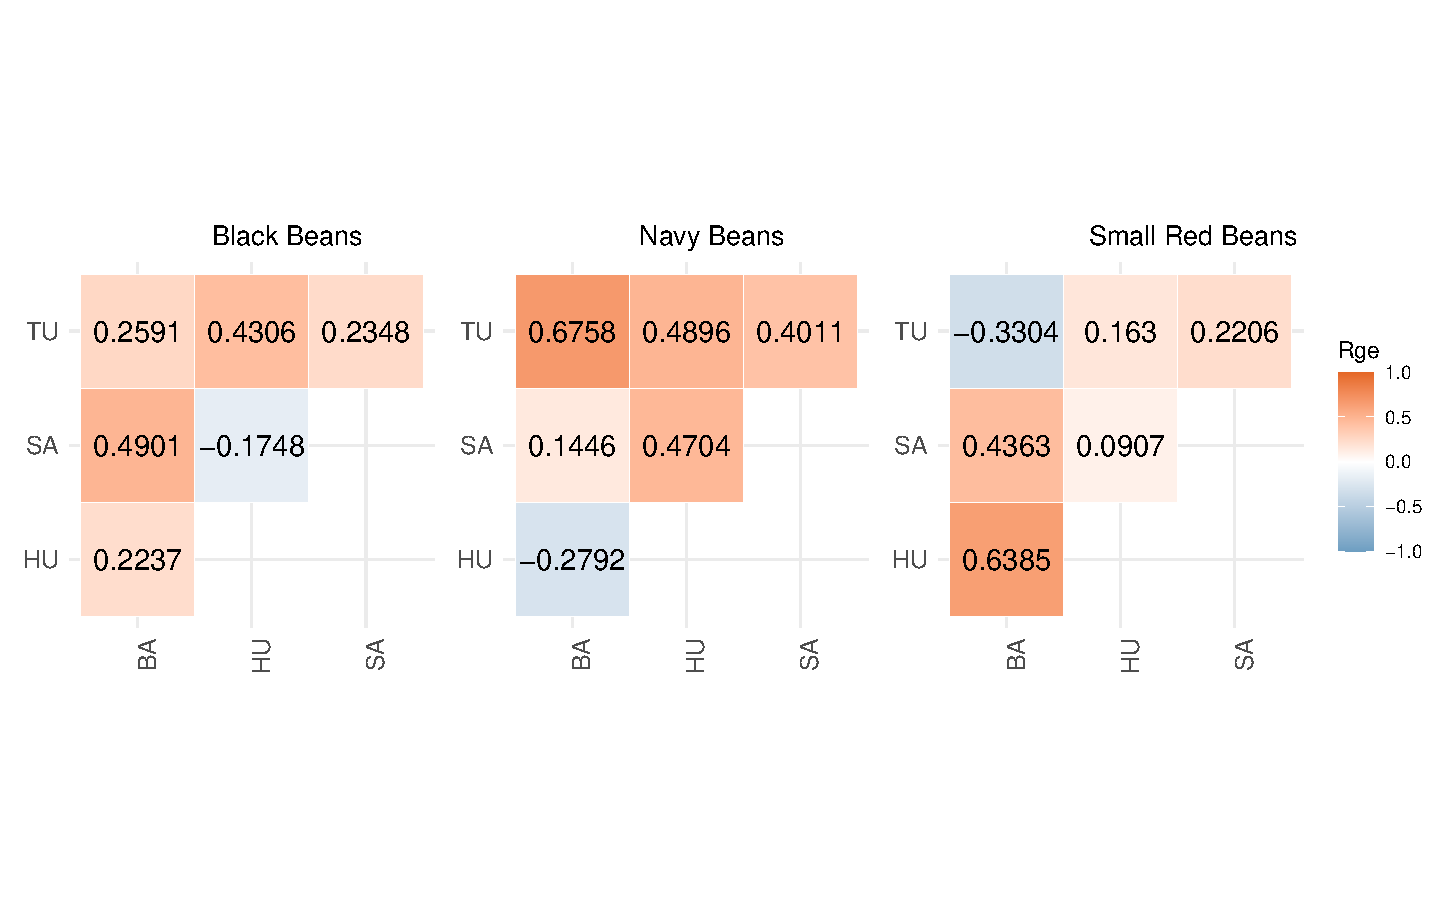
\includegraphics{figures/corr combined figure-1} \end{center}

\hypertarget{analyzing-met---gge}{%
\subsection{Analyzing MET - GGE}\label{analyzing-met---gge}}

Genotype plus Genotype-vs-Environment interaction (GGE) model has been
widely used to genotype evaluation and mega-environment identification
in multi-environment trials (MET). This model considers a GGE (i.e., G +
GE) biplot, which is constructed by the first two symmetrically scaled
principal components (PC1 and PC2) derived from singular value
decomposition of environment-centered MET data. The GGE biplot
graphically displays G plus GE of a MET in a way that facilitates visual
genotype evaluation and mega-environment identification
\href{GGE\%20Biplot\%20vs.\%20AMMI\%20Analysis\%20of\%20Genotype-by-Environment\%20Data}{@yanGGEBiplotVs2007}.

\hypertarget{gge-biplot-model}{%
\subsubsection{GGE biplot model}\label{gge-biplot-model}}

The mean yield of genotype \emph{i} in environment \emph{j} is commonly
described by a general linear model

\[
\hat y_{ij} + \mu + \alpha_i + \beta_j + \phi_{ij}
\] where \(\hat y_{ij}\) is the mean yield of genotype \emph{i} in
environment \emph{j}, \(i = 1, ... g; j = 1, ...e\) being \emph{g} and
\emph{e} the numbers of genotypes and environments, respectively;
\(\mu\) is the grand mean; \(\alpha_i\) is the main effect of the
genotype \emph{i}; \(\beta_j\) is the main effect of the environment
\emph{j}, and \(\phi_{ij}\) is the interaction effect between genotype
\emph{i} and environment \emph{j}. In the Genotype plus
Genotype-vs-Environment interaction (GGE) model the \(\alpha_i\) term is
is deleted from the above model and then the environment-centered data
matrix, \(\phi_{ij}\), is subjected to SVD
\href{GGE\%20biplot\%20analysis:\%20a\%20graphical\%20tool\%20for\%20breeders,\%20geneticists,\%20and\%20agronomists}{@yanGGEBiplotAnalysis2003}
and
\href{GGE\%20Biplot\%20vs.\%20AMMI\%20Analysis\%20of\%20Genotype-by-Environment\%20Data}{@yanGGEBiplotVs2007}.
Explicitly, we have

\[
{\phi_{ij} =  \hat y_{ij}} - \mu - \beta_j  = \sum\limits_{k = 1}^p \xi_{ik}^*\eta_{jk}^*
\]

where \(\xi_{ik}^* = \lambda_k^\alpha\xi_{ik}\);
\(\eta_{jk}^* = \lambda_k^{1-\alpha}\eta_{jk}\) being \(\lambda_k\) the
\emph{k}th eigenvalue from the SVD (\(k = 1, ...p\)), with
\(p \le min(e, g)\); \(\alpha\) is the the singular value partition
factor for the Principal Component (PC) \emph{k}; \(\xi_{ik}^*\) and
\(\eta_{jk}^*\) are the PC scores for genotype \emph{i} and environment
\emph{j}, respectively.

The function \texttt{gge()} from the R package \texttt{metan}
\href{Olivoto\%20et\%20al.,\%202019a}{@olivotoMeanPerformanceStability2019}
according to
\href{GGE\%20biplot\%20analysis:\%20a\%20graphical\%20tool\%20for\%20breeders,\%20geneticists,\%20and\%20agronomists}{@yanGGEBiplotAnalysis2003}
was deployed to produce the GGE model in this study.

\hypertarget{waasb-index}{%
\subsection{WAASB index}\label{waasb-index}}

The function \texttt{waasb()} function computes the Weighted Average of
the Absolute Scores considering all possible IPCA from the Singular
Value Decomposition of the BLUPs for genotype-vs-environment interaction
effects obtained by an Linear Mixed-effect Model
\href{Olivoto\%20et\%20al.,\%202019a}{@olivotoMeanPerformanceStability2019},
as follows:

\[
        WAASB_i  = 
        \sum_{k = 1}^{p} |IPCA_{ik} \times EP_k|/ \sum_{k = 1}^{p}EP_k
\]

where \(WAASB_i\) is the weighted average of absolute scores of the
\emph{i}th genotype; \(IPCA_{ik}\) is the scores of the \emph{i}th
genotype in the \emph{k}th IPCA; and \(EP_k\) is the explained variance
of the \emph{k}th PCA for \(k = 1,2,..,p\), \(p = min(g-1; e-1)\).

\hypertarget{waasby-index}{%
\subsection{WAASBY index}\label{waasby-index}}

\begin{itemize}
\tightlist
\item
  Simultaneous selection for mean performance and stability
\end{itemize}

The \textbf{waasby} index is used for genotype ranking considering both
the stability (\textbf{waasb}) and mean performance (\textbf{y}) based
on the following model
\href{Olivoto\%20et\%20al.,\%202019a}{@olivotoMeanPerformanceStability2019}.

\[
waasby_i = \frac{{\left( {r {Y_i} \times {\theta _Y}} \right) + \left( {r {W_i} \times {\theta _W}} \right)}}{{{\theta _Y} + {\theta _W}}}
\]

where \(waasby_i\) is the superiority index for the \emph{i}-th
genotype; \(rY_i\) and \(rW_i\) are the rescaled values (0-100) for the
response variable (y) and the stability (WAAS or WAASB), respectively;
\(\theta _Y\) and \(\theta_W\) are the weights for mean performance and
stability, respectively.

\hypertarget{appendix-d---r-codes}{%
\section{Appendix D - R codes}\label{appendix-d---r-codes}}

\hypertarget{met-analysis---market-class-combined}{%
\subsection{\texorpdfstring{MET analysis - \textbf{Market class
combined}}{MET analysis - Market class combined}}\label{met-analysis---market-class-combined}}

\hypertarget{met-analysis---asreml}{%
\subsubsection{MET analysis - ASReml}\label{met-analysis---asreml}}

Running MET using \texttt{ASReml} - only to comparison of variance
components with \texttt{metan} outputs

\begin{Shaded}
\begin{Highlighting}[]
\NormalTok{mod.met.asreml }\OtherTok{\textless{}{-}} \FunctionTok{asreml}\NormalTok{(}\AttributeTok{fixed =}\NormalTok{ yield }\SpecialCharTok{\textasciitilde{}}\NormalTok{ loc }\SpecialCharTok{+}\NormalTok{ loc}\SpecialCharTok{:}\NormalTok{rep,}
                \AttributeTok{random =} \SpecialCharTok{\textasciitilde{}}\NormalTok{ name }\SpecialCharTok{+}\NormalTok{ name}\SpecialCharTok{:}\NormalTok{loc,}
                \AttributeTok{data =}\NormalTok{ blues\_stage.I,}
                \AttributeTok{predict =} \FunctionTok{predict.asreml}\NormalTok{(}\AttributeTok{classify =} \StringTok{"name"}\NormalTok{),}
                \AttributeTok{trace =}\NormalTok{ F,}
                \AttributeTok{maxit =} \DecValTok{500}\NormalTok{)}
\NormalTok{summFix.met.asreml}\OtherTok{\textless{}{-}} \FunctionTok{data.frame}\NormalTok{(}\FunctionTok{wald}\NormalTok{(mod.met.asreml))}
\NormalTok{summFix.met.asreml}
\end{Highlighting}
\end{Shaded}

\global\setlength{\Oldarrayrulewidth}{\arrayrulewidth}

\global\setlength{\Oldtabcolsep}{\tabcolsep}

\setlength{\tabcolsep}{0pt}

\renewcommand*{\arraystretch}{1.5}



\providecommand{\ascline}[3]{\noalign{\global\arrayrulewidth #1}\arrayrulecolor[HTML]{#2}\cline{#3}}

\begin{longtable}[c]{|p{0.75in}|p{1.11in}|p{1.02in}|p{0.76in}}



\ascline{1.5pt}{666666}{1-4}

\multicolumn{1}{>{\raggedleft}m{\dimexpr 0.75in+0\tabcolsep}}{\textcolor[HTML]{000000}{\fontsize{9}{9}\selectfont{\global\setmainfont{Arial}{\textbf{Df}}}}} & \multicolumn{1}{>{\raggedleft}m{\dimexpr 1.11in+0\tabcolsep}}{\textcolor[HTML]{000000}{\fontsize{9}{9}\selectfont{\global\setmainfont{Arial}{\textbf{Sum.of.Sq}}}}} & \multicolumn{1}{>{\raggedleft}m{\dimexpr 1.02in+0\tabcolsep}}{\textcolor[HTML]{000000}{\fontsize{9}{9}\selectfont{\global\setmainfont{Arial}{\textbf{Wald.statistic}}}}} & \multicolumn{1}{>{\raggedleft}m{\dimexpr 0.76in+0\tabcolsep}}{\textcolor[HTML]{000000}{\fontsize{9}{9}\selectfont{\global\setmainfont{Arial}{\textbf{Pr.Chisq.}}}}} \\

\ascline{0.75pt}{666666}{1-4}



\multicolumn{1}{>{\raggedleft}m{\dimexpr 0.75in+0\tabcolsep}}{\textcolor[HTML]{999999}{\fontsize{9}{9}\selectfont{\global\setmainfont{Arial}{\textbf{numeric}}}}} & \multicolumn{1}{>{\raggedleft}m{\dimexpr 1.11in+0\tabcolsep}}{\textcolor[HTML]{999999}{\fontsize{9}{9}\selectfont{\global\setmainfont{Arial}{\textbf{numeric}}}}} & \multicolumn{1}{>{\raggedleft}m{\dimexpr 1.02in+0\tabcolsep}}{\textcolor[HTML]{999999}{\fontsize{9}{9}\selectfont{\global\setmainfont{Arial}{\textbf{numeric}}}}} & \multicolumn{1}{>{\raggedleft}m{\dimexpr 0.76in+0\tabcolsep}}{\textcolor[HTML]{999999}{\fontsize{9}{9}\selectfont{\global\setmainfont{Arial}{\textbf{numeric}}}}} \\

\ascline{1.5pt}{666666}{1-4}\endfirsthead

\ascline{1.5pt}{666666}{1-4}

\multicolumn{1}{>{\raggedleft}m{\dimexpr 0.75in+0\tabcolsep}}{\textcolor[HTML]{000000}{\fontsize{9}{9}\selectfont{\global\setmainfont{Arial}{\textbf{Df}}}}} & \multicolumn{1}{>{\raggedleft}m{\dimexpr 1.11in+0\tabcolsep}}{\textcolor[HTML]{000000}{\fontsize{9}{9}\selectfont{\global\setmainfont{Arial}{\textbf{Sum.of.Sq}}}}} & \multicolumn{1}{>{\raggedleft}m{\dimexpr 1.02in+0\tabcolsep}}{\textcolor[HTML]{000000}{\fontsize{9}{9}\selectfont{\global\setmainfont{Arial}{\textbf{Wald.statistic}}}}} & \multicolumn{1}{>{\raggedleft}m{\dimexpr 0.76in+0\tabcolsep}}{\textcolor[HTML]{000000}{\fontsize{9}{9}\selectfont{\global\setmainfont{Arial}{\textbf{Pr.Chisq.}}}}} \\

\ascline{0.75pt}{666666}{1-4}



\multicolumn{1}{>{\raggedleft}m{\dimexpr 0.75in+0\tabcolsep}}{\textcolor[HTML]{999999}{\fontsize{9}{9}\selectfont{\global\setmainfont{Arial}{\textbf{numeric}}}}} & \multicolumn{1}{>{\raggedleft}m{\dimexpr 1.11in+0\tabcolsep}}{\textcolor[HTML]{999999}{\fontsize{9}{9}\selectfont{\global\setmainfont{Arial}{\textbf{numeric}}}}} & \multicolumn{1}{>{\raggedleft}m{\dimexpr 1.02in+0\tabcolsep}}{\textcolor[HTML]{999999}{\fontsize{9}{9}\selectfont{\global\setmainfont{Arial}{\textbf{numeric}}}}} & \multicolumn{1}{>{\raggedleft}m{\dimexpr 0.76in+0\tabcolsep}}{\textcolor[HTML]{999999}{\fontsize{9}{9}\selectfont{\global\setmainfont{Arial}{\textbf{numeric}}}}} \\

\ascline{1.5pt}{666666}{1-4}\endhead



\multicolumn{4}{>{\raggedleft}m{\dimexpr 3.64in+6\tabcolsep}}{\textcolor[HTML]{000000}{\fontsize{9}{9}\selectfont{\global\setmainfont{Arial}{n:\ 4}}}} \\

\ascline{0.75pt}{666666}{1-4}\endfoot



\multicolumn{1}{>{\raggedleft}m{\dimexpr 0.75in+0\tabcolsep}}{\textcolor[HTML]{000000}{\fontsize{9}{9}\selectfont{\global\setmainfont{Arial}{1}}}} & \multicolumn{1}{>{\raggedleft}m{\dimexpr 1.11in+0\tabcolsep}}{\textcolor[HTML]{000000}{\fontsize{9}{9}\selectfont{\global\setmainfont{Arial}{2,721,855,097.2}}}} & \multicolumn{1}{>{\raggedleft}m{\dimexpr 1.02in+0\tabcolsep}}{\textcolor[HTML]{000000}{\fontsize{9}{9}\selectfont{\global\setmainfont{Arial}{15,045.0}}}} & \multicolumn{1}{>{\raggedleft}m{\dimexpr 0.76in+0\tabcolsep}}{\textcolor[HTML]{000000}{\fontsize{9}{9}\selectfont{\global\setmainfont{Arial}{0}}}} \\

\ascline{0.75pt}{666666}{1-4}



\multicolumn{1}{>{\raggedleft}m{\dimexpr 0.75in+0\tabcolsep}}{\textcolor[HTML]{000000}{\fontsize{9}{9}\selectfont{\global\setmainfont{Arial}{3}}}} & \multicolumn{1}{>{\raggedleft}m{\dimexpr 1.11in+0\tabcolsep}}{\textcolor[HTML]{000000}{\fontsize{9}{9}\selectfont{\global\setmainfont{Arial}{22,230,435.7}}}} & \multicolumn{1}{>{\raggedleft}m{\dimexpr 1.02in+0\tabcolsep}}{\textcolor[HTML]{000000}{\fontsize{9}{9}\selectfont{\global\setmainfont{Arial}{122.9}}}} & \multicolumn{1}{>{\raggedleft}m{\dimexpr 0.76in+0\tabcolsep}}{\textcolor[HTML]{000000}{\fontsize{9}{9}\selectfont{\global\setmainfont{Arial}{0}}}} \\

\ascline{0.75pt}{666666}{1-4}



\multicolumn{1}{>{\raggedleft}m{\dimexpr 0.75in+0\tabcolsep}}{\textcolor[HTML]{000000}{\fontsize{9}{9}\selectfont{\global\setmainfont{Arial}{12}}}} & \multicolumn{1}{>{\raggedleft}m{\dimexpr 1.11in+0\tabcolsep}}{\textcolor[HTML]{000000}{\fontsize{9}{9}\selectfont{\global\setmainfont{Arial}{32,105,353.5}}}} & \multicolumn{1}{>{\raggedleft}m{\dimexpr 1.02in+0\tabcolsep}}{\textcolor[HTML]{000000}{\fontsize{9}{9}\selectfont{\global\setmainfont{Arial}{177.5}}}} & \multicolumn{1}{>{\raggedleft}m{\dimexpr 0.76in+0\tabcolsep}}{\textcolor[HTML]{000000}{\fontsize{9}{9}\selectfont{\global\setmainfont{Arial}{0}}}} \\

\ascline{0.75pt}{666666}{1-4}



\multicolumn{1}{>{\raggedleft}m{\dimexpr 0.75in+0\tabcolsep}}{\textcolor[HTML]{000000}{\fontsize{9}{9}\selectfont{\global\setmainfont{Arial}{}}}} & \multicolumn{1}{>{\raggedleft}m{\dimexpr 1.11in+0\tabcolsep}}{\textcolor[HTML]{000000}{\fontsize{9}{9}\selectfont{\global\setmainfont{Arial}{180,914.2}}}} & \multicolumn{1}{>{\raggedleft}m{\dimexpr 1.02in+0\tabcolsep}}{\textcolor[HTML]{000000}{\fontsize{9}{9}\selectfont{\global\setmainfont{Arial}{}}}} & \multicolumn{1}{>{\raggedleft}m{\dimexpr 0.76in+0\tabcolsep}}{\textcolor[HTML]{000000}{\fontsize{9}{9}\selectfont{\global\setmainfont{Arial}{}}}} \\

\ascline{1.5pt}{666666}{1-4}



\end{longtable}



\arrayrulecolor[HTML]{000000}

\global\setlength{\arrayrulewidth}{\Oldarrayrulewidth}

\global\setlength{\tabcolsep}{\Oldtabcolsep}

\renewcommand*{\arraystretch}{1}

\begin{Shaded}
\begin{Highlighting}[]
\NormalTok{summ.met.asreml}\OtherTok{\textless{}{-}} \FunctionTok{data.frame}\NormalTok{(}\FunctionTok{summary.asreml}\NormalTok{(mod.met.asreml)}\SpecialCharTok{$}\NormalTok{varcomp)}
\NormalTok{summ.met.asreml}
\end{Highlighting}
\end{Shaded}

\global\setlength{\Oldarrayrulewidth}{\arrayrulewidth}

\global\setlength{\Oldtabcolsep}{\tabcolsep}

\setlength{\tabcolsep}{0pt}

\renewcommand*{\arraystretch}{1.5}



\providecommand{\ascline}[3]{\noalign{\global\arrayrulewidth #1}\arrayrulecolor[HTML]{#2}\cline{#3}}

\begin{longtable}[c]{|p{0.88in}|p{0.75in}|p{0.75in}|p{0.77in}|p{0.75in}}



\ascline{1.5pt}{666666}{1-5}

\multicolumn{1}{>{\raggedleft}m{\dimexpr 0.88in+0\tabcolsep}}{\textcolor[HTML]{000000}{\fontsize{9}{9}\selectfont{\global\setmainfont{Arial}{\textbf{component}}}}} & \multicolumn{1}{>{\raggedleft}m{\dimexpr 0.75in+0\tabcolsep}}{\textcolor[HTML]{000000}{\fontsize{9}{9}\selectfont{\global\setmainfont{Arial}{\textbf{std.error}}}}} & \multicolumn{1}{>{\raggedleft}m{\dimexpr 0.75in+0\tabcolsep}}{\textcolor[HTML]{000000}{\fontsize{9}{9}\selectfont{\global\setmainfont{Arial}{\textbf{z.ratio}}}}} & \multicolumn{1}{>{\raggedright}m{\dimexpr 0.77in+0\tabcolsep}}{\textcolor[HTML]{000000}{\fontsize{9}{9}\selectfont{\global\setmainfont{Arial}{\textbf{bound}}}}} & \multicolumn{1}{>{\raggedleft}m{\dimexpr 0.75in+0\tabcolsep}}{\textcolor[HTML]{000000}{\fontsize{9}{9}\selectfont{\global\setmainfont{Arial}{\textbf{X.ch}}}}} \\

\ascline{0.75pt}{666666}{1-5}



\multicolumn{1}{>{\raggedleft}m{\dimexpr 0.88in+0\tabcolsep}}{\textcolor[HTML]{999999}{\fontsize{9}{9}\selectfont{\global\setmainfont{Arial}{\textbf{numeric}}}}} & \multicolumn{1}{>{\raggedleft}m{\dimexpr 0.75in+0\tabcolsep}}{\textcolor[HTML]{999999}{\fontsize{9}{9}\selectfont{\global\setmainfont{Arial}{\textbf{numeric}}}}} & \multicolumn{1}{>{\raggedleft}m{\dimexpr 0.75in+0\tabcolsep}}{\textcolor[HTML]{999999}{\fontsize{9}{9}\selectfont{\global\setmainfont{Arial}{\textbf{numeric}}}}} & \multicolumn{1}{>{\raggedright}m{\dimexpr 0.77in+0\tabcolsep}}{\textcolor[HTML]{999999}{\fontsize{9}{9}\selectfont{\global\setmainfont{Arial}{\textbf{character}}}}} & \multicolumn{1}{>{\raggedleft}m{\dimexpr 0.75in+0\tabcolsep}}{\textcolor[HTML]{999999}{\fontsize{9}{9}\selectfont{\global\setmainfont{Arial}{\textbf{numeric}}}}} \\

\ascline{1.5pt}{666666}{1-5}\endfirsthead

\ascline{1.5pt}{666666}{1-5}

\multicolumn{1}{>{\raggedleft}m{\dimexpr 0.88in+0\tabcolsep}}{\textcolor[HTML]{000000}{\fontsize{9}{9}\selectfont{\global\setmainfont{Arial}{\textbf{component}}}}} & \multicolumn{1}{>{\raggedleft}m{\dimexpr 0.75in+0\tabcolsep}}{\textcolor[HTML]{000000}{\fontsize{9}{9}\selectfont{\global\setmainfont{Arial}{\textbf{std.error}}}}} & \multicolumn{1}{>{\raggedleft}m{\dimexpr 0.75in+0\tabcolsep}}{\textcolor[HTML]{000000}{\fontsize{9}{9}\selectfont{\global\setmainfont{Arial}{\textbf{z.ratio}}}}} & \multicolumn{1}{>{\raggedright}m{\dimexpr 0.77in+0\tabcolsep}}{\textcolor[HTML]{000000}{\fontsize{9}{9}\selectfont{\global\setmainfont{Arial}{\textbf{bound}}}}} & \multicolumn{1}{>{\raggedleft}m{\dimexpr 0.75in+0\tabcolsep}}{\textcolor[HTML]{000000}{\fontsize{9}{9}\selectfont{\global\setmainfont{Arial}{\textbf{X.ch}}}}} \\

\ascline{0.75pt}{666666}{1-5}



\multicolumn{1}{>{\raggedleft}m{\dimexpr 0.88in+0\tabcolsep}}{\textcolor[HTML]{999999}{\fontsize{9}{9}\selectfont{\global\setmainfont{Arial}{\textbf{numeric}}}}} & \multicolumn{1}{>{\raggedleft}m{\dimexpr 0.75in+0\tabcolsep}}{\textcolor[HTML]{999999}{\fontsize{9}{9}\selectfont{\global\setmainfont{Arial}{\textbf{numeric}}}}} & \multicolumn{1}{>{\raggedleft}m{\dimexpr 0.75in+0\tabcolsep}}{\textcolor[HTML]{999999}{\fontsize{9}{9}\selectfont{\global\setmainfont{Arial}{\textbf{numeric}}}}} & \multicolumn{1}{>{\raggedright}m{\dimexpr 0.77in+0\tabcolsep}}{\textcolor[HTML]{999999}{\fontsize{9}{9}\selectfont{\global\setmainfont{Arial}{\textbf{character}}}}} & \multicolumn{1}{>{\raggedleft}m{\dimexpr 0.75in+0\tabcolsep}}{\textcolor[HTML]{999999}{\fontsize{9}{9}\selectfont{\global\setmainfont{Arial}{\textbf{numeric}}}}} \\

\ascline{1.5pt}{666666}{1-5}\endhead



\multicolumn{5}{>{\raggedleft}m{\dimexpr 3.91in+8\tabcolsep}}{\textcolor[HTML]{000000}{\fontsize{9}{9}\selectfont{\global\setmainfont{Arial}{n:\ 3}}}} \\

\ascline{0.75pt}{666666}{1-5}\endfoot



\multicolumn{1}{>{\raggedleft}m{\dimexpr 0.88in+0\tabcolsep}}{\textcolor[HTML]{000000}{\fontsize{9}{9}\selectfont{\global\setmainfont{Arial}{63,149.3}}}} & \multicolumn{1}{>{\raggedleft}m{\dimexpr 0.75in+0\tabcolsep}}{\textcolor[HTML]{000000}{\fontsize{9}{9}\selectfont{\global\setmainfont{Arial}{11,854.7}}}} & \multicolumn{1}{>{\raggedleft}m{\dimexpr 0.75in+0\tabcolsep}}{\textcolor[HTML]{000000}{\fontsize{9}{9}\selectfont{\global\setmainfont{Arial}{5.3}}}} & \multicolumn{1}{>{\raggedright}m{\dimexpr 0.77in+0\tabcolsep}}{\textcolor[HTML]{000000}{\fontsize{9}{9}\selectfont{\global\setmainfont{Arial}{P}}}} & \multicolumn{1}{>{\raggedleft}m{\dimexpr 0.75in+0\tabcolsep}}{\textcolor[HTML]{000000}{\fontsize{9}{9}\selectfont{\global\setmainfont{Arial}{0}}}} \\

\ascline{0.75pt}{666666}{1-5}



\multicolumn{1}{>{\raggedleft}m{\dimexpr 0.88in+0\tabcolsep}}{\textcolor[HTML]{000000}{\fontsize{9}{9}\selectfont{\global\setmainfont{Arial}{116,086.7}}}} & \multicolumn{1}{>{\raggedleft}m{\dimexpr 0.75in+0\tabcolsep}}{\textcolor[HTML]{000000}{\fontsize{9}{9}\selectfont{\global\setmainfont{Arial}{10,681.0}}}} & \multicolumn{1}{>{\raggedleft}m{\dimexpr 0.75in+0\tabcolsep}}{\textcolor[HTML]{000000}{\fontsize{9}{9}\selectfont{\global\setmainfont{Arial}{10.9}}}} & \multicolumn{1}{>{\raggedright}m{\dimexpr 0.77in+0\tabcolsep}}{\textcolor[HTML]{000000}{\fontsize{9}{9}\selectfont{\global\setmainfont{Arial}{P}}}} & \multicolumn{1}{>{\raggedleft}m{\dimexpr 0.75in+0\tabcolsep}}{\textcolor[HTML]{000000}{\fontsize{9}{9}\selectfont{\global\setmainfont{Arial}{0}}}} \\

\ascline{0.75pt}{666666}{1-5}



\multicolumn{1}{>{\raggedleft}m{\dimexpr 0.88in+0\tabcolsep}}{\textcolor[HTML]{000000}{\fontsize{9}{9}\selectfont{\global\setmainfont{Arial}{180,914.2}}}} & \multicolumn{1}{>{\raggedleft}m{\dimexpr 0.75in+0\tabcolsep}}{\textcolor[HTML]{000000}{\fontsize{9}{9}\selectfont{\global\setmainfont{Arial}{5,991.2}}}} & \multicolumn{1}{>{\raggedleft}m{\dimexpr 0.75in+0\tabcolsep}}{\textcolor[HTML]{000000}{\fontsize{9}{9}\selectfont{\global\setmainfont{Arial}{30.2}}}} & \multicolumn{1}{>{\raggedright}m{\dimexpr 0.77in+0\tabcolsep}}{\textcolor[HTML]{000000}{\fontsize{9}{9}\selectfont{\global\setmainfont{Arial}{P}}}} & \multicolumn{1}{>{\raggedleft}m{\dimexpr 0.75in+0\tabcolsep}}{\textcolor[HTML]{000000}{\fontsize{9}{9}\selectfont{\global\setmainfont{Arial}{0}}}} \\

\ascline{1.5pt}{666666}{1-5}



\end{longtable}



\arrayrulecolor[HTML]{000000}

\global\setlength{\arrayrulewidth}{\Oldarrayrulewidth}

\global\setlength{\tabcolsep}{\Oldtabcolsep}

\renewcommand*{\arraystretch}{1}

\begin{Shaded}
\begin{Highlighting}[]
\CommentTok{\#print(summary.asreml(mod.met.asreml)$bic)}
\CommentTok{\#mod.met.asreml\textless{}{-} data.table((mod.met.asreml$predictions$pvals[1:3]))}
\NormalTok{mod.met.asreml2 }\OtherTok{\textless{}{-}} \FunctionTok{data.table}\NormalTok{(}\FunctionTok{matrix}\NormalTok{(}\FunctionTok{unlist}\NormalTok{(mod.met.asreml}\SpecialCharTok{$}\NormalTok{predictions}\SpecialCharTok{$}\NormalTok{pvals[}\DecValTok{1}\SpecialCharTok{:}\DecValTok{3}\NormalTok{]),}
 \AttributeTok{ncol=}\DecValTok{3}\NormalTok{))}
\FunctionTok{names}\NormalTok{(mod.met.asreml2) }\OtherTok{\textless{}{-}} \FunctionTok{c}\NormalTok{(}\StringTok{"name"}\NormalTok{, }\StringTok{"yield\_BLUPS\_MET"}\NormalTok{, }\StringTok{"SE"}\NormalTok{)}
\NormalTok{mod.met.asreml2}\SpecialCharTok{$}\NormalTok{yield\_BLUPS\_MET}\OtherTok{\textless{}{-}}\FunctionTok{as.numeric}\NormalTok{(mod.met.asreml2}\SpecialCharTok{$}\NormalTok{yield\_BLUPS\_MET)}
\NormalTok{mod.met.asreml2}\SpecialCharTok{$}\NormalTok{SE}\OtherTok{\textless{}{-}}\FunctionTok{as.numeric}\NormalTok{(mod.met.asreml2}\SpecialCharTok{$}\NormalTok{SE)}
\end{Highlighting}
\end{Shaded}

\hypertarget{met-analysis---lme4}{%
\subsubsection{MET analysis - lme4}\label{met-analysis---lme4}}

Running MET using \texttt{metan} R package
\href{Olivoto\%20et\%20al.,\%202019a}{@olivotoMeanPerformanceStability2019}.

\begin{Shaded}
\begin{Highlighting}[]
\NormalTok{mixed\_mod}\OtherTok{\textless{}{-}} 
   \FunctionTok{gamem\_met}\NormalTok{(blues\_stage.I,}
             \AttributeTok{env =}\NormalTok{ loc,}
             \AttributeTok{gen =}\NormalTok{ name,}
             \AttributeTok{rep =}\NormalTok{ rep,}
             \AttributeTok{resp =}\NormalTok{ yield,}
             \AttributeTok{random =} \StringTok{"gen"}\NormalTok{, }\CommentTok{\#Default}
             \AttributeTok{verbose =} \ConstantTok{TRUE}\NormalTok{) }\CommentTok{\#Default}
\end{Highlighting}
\end{Shaded}

Evaluating trait yield
\textbar=================================================================================================================================================================================================\textbar{}
100\% 00:00:08

\begin{verbatim}
#> Method: REML/BLUP
\end{verbatim}

\begin{verbatim}
#> Random effects: GEN, GEN:ENV
\end{verbatim}

\begin{verbatim}
#> Fixed effects: ENV, REP(ENV)
\end{verbatim}

\begin{verbatim}
#> Denominador DF: Satterthwaite's method
\end{verbatim}

\begin{longtable}[]{@{}
  >{\raggedright\arraybackslash}p{(\columnwidth - 0\tabcolsep) * \real{1.0000}}@{}}
\toprule\noalign{}
\begin{minipage}[b]{\linewidth}\raggedright
P-values for Likelihood Ratio Test of the analyzed traits
\end{minipage} \\
\midrule\noalign{}
\endhead
\bottomrule\noalign{}
\endlastfoot
model yield COMPLETE NA GEN 1.18e-14 GEN:ENV 1.51e-75 \\
\end{longtable}

All variables with significant (p \textless{} 0.05)
genotype-vs-environment interaction

\hypertarget{printing-the-model-outputs}{%
\subsubsection{Printing the model
outputs}\label{printing-the-model-outputs}}

\hypertarget{likelihood-ratio-tests}{%
\paragraph{Likelihood Ratio Tests}\label{likelihood-ratio-tests}}

\begin{itemize}
\tightlist
\item
  The output \texttt{LRT} contains the Likelihood Ratio Tests for
  genotype and genotype-vs-environment random effects.
\end{itemize}

\begin{Shaded}
\begin{Highlighting}[]
\NormalTok{data\_mod\_bb\_test }\OtherTok{\textless{}{-}} \FunctionTok{get\_model\_data}\NormalTok{(mixed\_mod, }\StringTok{"lrt"}\NormalTok{)}
\end{Highlighting}
\end{Shaded}

\begin{verbatim}
#> Class of the model: waasb
\end{verbatim}

\begin{verbatim}
#> Variable extracted: lrt
\end{verbatim}

\begin{Shaded}
\begin{Highlighting}[]
\NormalTok{data\_mod\_bb\_test}
\end{Highlighting}
\end{Shaded}

\global\setlength{\Oldarrayrulewidth}{\arrayrulewidth}

\global\setlength{\Oldtabcolsep}{\tabcolsep}

\setlength{\tabcolsep}{0pt}

\renewcommand*{\arraystretch}{1.5}



\providecommand{\ascline}[3]{\noalign{\global\arrayrulewidth #1}\arrayrulecolor[HTML]{#2}\cline{#3}}

\begin{longtable}[c]{|p{0.77in}|p{0.77in}|p{0.75in}|p{0.75in}|p{0.75in}|p{0.75in}|p{0.75in}|p{0.85in}}



\ascline{1.5pt}{666666}{1-8}

\multicolumn{1}{>{\raggedright}m{\dimexpr 0.77in+0\tabcolsep}}{\textcolor[HTML]{000000}{\fontsize{9}{9}\selectfont{\global\setmainfont{Arial}{\textbf{VAR}}}}} & \multicolumn{1}{>{\raggedright}m{\dimexpr 0.77in+0\tabcolsep}}{\textcolor[HTML]{000000}{\fontsize{9}{9}\selectfont{\global\setmainfont{Arial}{\textbf{model}}}}} & \multicolumn{1}{>{\raggedleft}m{\dimexpr 0.75in+0\tabcolsep}}{\textcolor[HTML]{000000}{\fontsize{9}{9}\selectfont{\global\setmainfont{Arial}{\textbf{npar}}}}} & \multicolumn{1}{>{\raggedleft}m{\dimexpr 0.75in+0\tabcolsep}}{\textcolor[HTML]{000000}{\fontsize{9}{9}\selectfont{\global\setmainfont{Arial}{\textbf{logLik}}}}} & \multicolumn{1}{>{\raggedleft}m{\dimexpr 0.75in+0\tabcolsep}}{\textcolor[HTML]{000000}{\fontsize{9}{9}\selectfont{\global\setmainfont{Arial}{\textbf{AIC}}}}} & \multicolumn{1}{>{\raggedleft}m{\dimexpr 0.75in+0\tabcolsep}}{\textcolor[HTML]{000000}{\fontsize{9}{9}\selectfont{\global\setmainfont{Arial}{\textbf{LRT}}}}} & \multicolumn{1}{>{\raggedleft}m{\dimexpr 0.75in+0\tabcolsep}}{\textcolor[HTML]{000000}{\fontsize{9}{9}\selectfont{\global\setmainfont{Arial}{\textbf{Df}}}}} & \multicolumn{1}{>{\raggedleft}m{\dimexpr 0.85in+0\tabcolsep}}{\textcolor[HTML]{000000}{\fontsize{9}{9}\selectfont{\global\setmainfont{Arial}{\textbf{Pr(>Chisq)}}}}} \\

\ascline{0.75pt}{666666}{1-8}



\multicolumn{1}{>{\raggedright}m{\dimexpr 0.77in+0\tabcolsep}}{\textcolor[HTML]{999999}{\fontsize{9}{9}\selectfont{\global\setmainfont{Arial}{\textbf{character}}}}} & \multicolumn{1}{>{\raggedright}m{\dimexpr 0.77in+0\tabcolsep}}{\textcolor[HTML]{999999}{\fontsize{9}{9}\selectfont{\global\setmainfont{Arial}{\textbf{character}}}}} & \multicolumn{1}{>{\raggedleft}m{\dimexpr 0.75in+0\tabcolsep}}{\textcolor[HTML]{999999}{\fontsize{9}{9}\selectfont{\global\setmainfont{Arial}{\textbf{integer}}}}} & \multicolumn{1}{>{\raggedleft}m{\dimexpr 0.75in+0\tabcolsep}}{\textcolor[HTML]{999999}{\fontsize{9}{9}\selectfont{\global\setmainfont{Arial}{\textbf{numeric}}}}} & \multicolumn{1}{>{\raggedleft}m{\dimexpr 0.75in+0\tabcolsep}}{\textcolor[HTML]{999999}{\fontsize{9}{9}\selectfont{\global\setmainfont{Arial}{\textbf{numeric}}}}} & \multicolumn{1}{>{\raggedleft}m{\dimexpr 0.75in+0\tabcolsep}}{\textcolor[HTML]{999999}{\fontsize{9}{9}\selectfont{\global\setmainfont{Arial}{\textbf{numeric}}}}} & \multicolumn{1}{>{\raggedleft}m{\dimexpr 0.75in+0\tabcolsep}}{\textcolor[HTML]{999999}{\fontsize{9}{9}\selectfont{\global\setmainfont{Arial}{\textbf{numeric}}}}} & \multicolumn{1}{>{\raggedleft}m{\dimexpr 0.85in+0\tabcolsep}}{\textcolor[HTML]{999999}{\fontsize{9}{9}\selectfont{\global\setmainfont{Arial}{\textbf{numeric}}}}} \\

\ascline{1.5pt}{666666}{1-8}\endfirsthead

\ascline{1.5pt}{666666}{1-8}

\multicolumn{1}{>{\raggedright}m{\dimexpr 0.77in+0\tabcolsep}}{\textcolor[HTML]{000000}{\fontsize{9}{9}\selectfont{\global\setmainfont{Arial}{\textbf{VAR}}}}} & \multicolumn{1}{>{\raggedright}m{\dimexpr 0.77in+0\tabcolsep}}{\textcolor[HTML]{000000}{\fontsize{9}{9}\selectfont{\global\setmainfont{Arial}{\textbf{model}}}}} & \multicolumn{1}{>{\raggedleft}m{\dimexpr 0.75in+0\tabcolsep}}{\textcolor[HTML]{000000}{\fontsize{9}{9}\selectfont{\global\setmainfont{Arial}{\textbf{npar}}}}} & \multicolumn{1}{>{\raggedleft}m{\dimexpr 0.75in+0\tabcolsep}}{\textcolor[HTML]{000000}{\fontsize{9}{9}\selectfont{\global\setmainfont{Arial}{\textbf{logLik}}}}} & \multicolumn{1}{>{\raggedleft}m{\dimexpr 0.75in+0\tabcolsep}}{\textcolor[HTML]{000000}{\fontsize{9}{9}\selectfont{\global\setmainfont{Arial}{\textbf{AIC}}}}} & \multicolumn{1}{>{\raggedleft}m{\dimexpr 0.75in+0\tabcolsep}}{\textcolor[HTML]{000000}{\fontsize{9}{9}\selectfont{\global\setmainfont{Arial}{\textbf{LRT}}}}} & \multicolumn{1}{>{\raggedleft}m{\dimexpr 0.75in+0\tabcolsep}}{\textcolor[HTML]{000000}{\fontsize{9}{9}\selectfont{\global\setmainfont{Arial}{\textbf{Df}}}}} & \multicolumn{1}{>{\raggedleft}m{\dimexpr 0.85in+0\tabcolsep}}{\textcolor[HTML]{000000}{\fontsize{9}{9}\selectfont{\global\setmainfont{Arial}{\textbf{Pr(>Chisq)}}}}} \\

\ascline{0.75pt}{666666}{1-8}



\multicolumn{1}{>{\raggedright}m{\dimexpr 0.77in+0\tabcolsep}}{\textcolor[HTML]{999999}{\fontsize{9}{9}\selectfont{\global\setmainfont{Arial}{\textbf{character}}}}} & \multicolumn{1}{>{\raggedright}m{\dimexpr 0.77in+0\tabcolsep}}{\textcolor[HTML]{999999}{\fontsize{9}{9}\selectfont{\global\setmainfont{Arial}{\textbf{character}}}}} & \multicolumn{1}{>{\raggedleft}m{\dimexpr 0.75in+0\tabcolsep}}{\textcolor[HTML]{999999}{\fontsize{9}{9}\selectfont{\global\setmainfont{Arial}{\textbf{integer}}}}} & \multicolumn{1}{>{\raggedleft}m{\dimexpr 0.75in+0\tabcolsep}}{\textcolor[HTML]{999999}{\fontsize{9}{9}\selectfont{\global\setmainfont{Arial}{\textbf{numeric}}}}} & \multicolumn{1}{>{\raggedleft}m{\dimexpr 0.75in+0\tabcolsep}}{\textcolor[HTML]{999999}{\fontsize{9}{9}\selectfont{\global\setmainfont{Arial}{\textbf{numeric}}}}} & \multicolumn{1}{>{\raggedleft}m{\dimexpr 0.75in+0\tabcolsep}}{\textcolor[HTML]{999999}{\fontsize{9}{9}\selectfont{\global\setmainfont{Arial}{\textbf{numeric}}}}} & \multicolumn{1}{>{\raggedleft}m{\dimexpr 0.75in+0\tabcolsep}}{\textcolor[HTML]{999999}{\fontsize{9}{9}\selectfont{\global\setmainfont{Arial}{\textbf{numeric}}}}} & \multicolumn{1}{>{\raggedleft}m{\dimexpr 0.85in+0\tabcolsep}}{\textcolor[HTML]{999999}{\fontsize{9}{9}\selectfont{\global\setmainfont{Arial}{\textbf{numeric}}}}} \\

\ascline{1.5pt}{666666}{1-8}\endhead



\multicolumn{8}{>{\raggedright}m{\dimexpr 6.14in+14\tabcolsep}}{\textcolor[HTML]{000000}{\fontsize{9}{9}\selectfont{\global\setmainfont{Arial}{n:\ 2}}}} \\

\ascline{0.75pt}{666666}{1-8}\endfoot



\multicolumn{1}{>{\raggedright}m{\dimexpr 0.77in+0\tabcolsep}}{\textcolor[HTML]{000000}{\fontsize{9}{9}\selectfont{\global\setmainfont{Arial}{yield}}}} & \multicolumn{1}{>{\raggedright}m{\dimexpr 0.77in+0\tabcolsep}}{\textcolor[HTML]{000000}{\fontsize{9}{9}\selectfont{\global\setmainfont{Arial}{GEN}}}} & \multicolumn{1}{>{\raggedleft}m{\dimexpr 0.75in+0\tabcolsep}}{\textcolor[HTML]{000000}{\fontsize{9}{9}\selectfont{\global\setmainfont{Arial}{18}}}} & \multicolumn{1}{>{\raggedleft}m{\dimexpr 0.75in+0\tabcolsep}}{\textcolor[HTML]{000000}{\fontsize{9}{9}\selectfont{\global\setmainfont{Arial}{-19,093.2}}}} & \multicolumn{1}{>{\raggedleft}m{\dimexpr 0.75in+0\tabcolsep}}{\textcolor[HTML]{000000}{\fontsize{9}{9}\selectfont{\global\setmainfont{Arial}{38,222.5}}}} & \multicolumn{1}{>{\raggedleft}m{\dimexpr 0.75in+0\tabcolsep}}{\textcolor[HTML]{000000}{\fontsize{9}{9}\selectfont{\global\setmainfont{Arial}{59.6}}}} & \multicolumn{1}{>{\raggedleft}m{\dimexpr 0.75in+0\tabcolsep}}{\textcolor[HTML]{000000}{\fontsize{9}{9}\selectfont{\global\setmainfont{Arial}{1}}}} & \multicolumn{1}{>{\raggedleft}m{\dimexpr 0.85in+0\tabcolsep}}{\textcolor[HTML]{000000}{\fontsize{9}{9}\selectfont{\global\setmainfont{Arial}{0}}}} \\

\ascline{0.75pt}{666666}{1-8}



\multicolumn{1}{>{\raggedright}m{\dimexpr 0.77in+0\tabcolsep}}{\textcolor[HTML]{000000}{\fontsize{9}{9}\selectfont{\global\setmainfont{Arial}{yield}}}} & \multicolumn{1}{>{\raggedright}m{\dimexpr 0.77in+0\tabcolsep}}{\textcolor[HTML]{000000}{\fontsize{9}{9}\selectfont{\global\setmainfont{Arial}{GEN:ENV}}}} & \multicolumn{1}{>{\raggedleft}m{\dimexpr 0.75in+0\tabcolsep}}{\textcolor[HTML]{000000}{\fontsize{9}{9}\selectfont{\global\setmainfont{Arial}{18}}}} & \multicolumn{1}{>{\raggedleft}m{\dimexpr 0.75in+0\tabcolsep}}{\textcolor[HTML]{000000}{\fontsize{9}{9}\selectfont{\global\setmainfont{Arial}{-19,232.6}}}} & \multicolumn{1}{>{\raggedleft}m{\dimexpr 0.75in+0\tabcolsep}}{\textcolor[HTML]{000000}{\fontsize{9}{9}\selectfont{\global\setmainfont{Arial}{38,501.2}}}} & \multicolumn{1}{>{\raggedleft}m{\dimexpr 0.75in+0\tabcolsep}}{\textcolor[HTML]{000000}{\fontsize{9}{9}\selectfont{\global\setmainfont{Arial}{338.3}}}} & \multicolumn{1}{>{\raggedleft}m{\dimexpr 0.75in+0\tabcolsep}}{\textcolor[HTML]{000000}{\fontsize{9}{9}\selectfont{\global\setmainfont{Arial}{1}}}} & \multicolumn{1}{>{\raggedleft}m{\dimexpr 0.85in+0\tabcolsep}}{\textcolor[HTML]{000000}{\fontsize{9}{9}\selectfont{\global\setmainfont{Arial}{0}}}} \\

\ascline{1.5pt}{666666}{1-8}



\end{longtable}



\arrayrulecolor[HTML]{000000}

\global\setlength{\arrayrulewidth}{\Oldarrayrulewidth}

\global\setlength{\tabcolsep}{\Oldtabcolsep}

\renewcommand*{\arraystretch}{1}

\begin{Shaded}
\begin{Highlighting}[]
\CommentTok{\#customize the display of numbers and other data in a tibble}
\CommentTok{\# old \textless{}{-} options(pillar.sigfig = 6)}
\CommentTok{\# }
\CommentTok{\# blues\_stage.I \%\textgreater{}\% }
\CommentTok{\#   group\_by(loc) \%\textgreater{}\% }
\CommentTok{\#   dplyr::summarise(Mean = mean(yield, na.rm = TRUE))}
\end{Highlighting}
\end{Shaded}

\hypertarget{detailed-parameters}{%
\paragraph{Detailed parameters}\label{detailed-parameters}}

\begin{Shaded}
\begin{Highlighting}[]
\NormalTok{data\_mod\_bb\_det }\OtherTok{\textless{}{-}} \FunctionTok{get\_model\_data}\NormalTok{(mixed\_mod, }\StringTok{"details"}\NormalTok{)}
\end{Highlighting}
\end{Shaded}

\begin{verbatim}
#> Class of the model: waasb
\end{verbatim}

\begin{verbatim}
#> Variable extracted: details
\end{verbatim}

\begin{Shaded}
\begin{Highlighting}[]
\NormalTok{data\_mod\_bb\_det}
\end{Highlighting}
\end{Shaded}

\global\setlength{\Oldarrayrulewidth}{\arrayrulewidth}

\global\setlength{\Oldtabcolsep}{\tabcolsep}

\setlength{\tabcolsep}{0pt}

\renewcommand*{\arraystretch}{1.5}



\providecommand{\ascline}[3]{\noalign{\global\arrayrulewidth #1}\arrayrulecolor[HTML]{#2}\cline{#3}}

\begin{longtable}[c]{|p{0.89in}|p{1.35in}}



\ascline{1.5pt}{666666}{1-2}

\multicolumn{1}{>{\raggedright}m{\dimexpr 0.89in+0\tabcolsep}}{\textcolor[HTML]{000000}{\fontsize{9}{9}\selectfont{\global\setmainfont{Arial}{\textbf{Parameters}}}}} & \multicolumn{1}{>{\raggedright}m{\dimexpr 1.35in+0\tabcolsep}}{\textcolor[HTML]{000000}{\fontsize{9}{9}\selectfont{\global\setmainfont{Arial}{\textbf{yield}}}}} \\

\ascline{0.75pt}{666666}{1-2}



\multicolumn{1}{>{\raggedright}m{\dimexpr 0.89in+0\tabcolsep}}{\textcolor[HTML]{999999}{\fontsize{9}{9}\selectfont{\global\setmainfont{Arial}{\textbf{character}}}}} & \multicolumn{1}{>{\raggedright}m{\dimexpr 1.35in+0\tabcolsep}}{\textcolor[HTML]{999999}{\fontsize{9}{9}\selectfont{\global\setmainfont{Arial}{\textbf{character}}}}} \\

\ascline{1.5pt}{666666}{1-2}\endfirsthead

\ascline{1.5pt}{666666}{1-2}

\multicolumn{1}{>{\raggedright}m{\dimexpr 0.89in+0\tabcolsep}}{\textcolor[HTML]{000000}{\fontsize{9}{9}\selectfont{\global\setmainfont{Arial}{\textbf{Parameters}}}}} & \multicolumn{1}{>{\raggedright}m{\dimexpr 1.35in+0\tabcolsep}}{\textcolor[HTML]{000000}{\fontsize{9}{9}\selectfont{\global\setmainfont{Arial}{\textbf{yield}}}}} \\

\ascline{0.75pt}{666666}{1-2}



\multicolumn{1}{>{\raggedright}m{\dimexpr 0.89in+0\tabcolsep}}{\textcolor[HTML]{999999}{\fontsize{9}{9}\selectfont{\global\setmainfont{Arial}{\textbf{character}}}}} & \multicolumn{1}{>{\raggedright}m{\dimexpr 1.35in+0\tabcolsep}}{\textcolor[HTML]{999999}{\fontsize{9}{9}\selectfont{\global\setmainfont{Arial}{\textbf{character}}}}} \\

\ascline{1.5pt}{666666}{1-2}\endhead



\multicolumn{2}{>{\raggedright}m{\dimexpr 2.24in+2\tabcolsep}}{\textcolor[HTML]{000000}{\fontsize{9}{9}\selectfont{\global\setmainfont{Arial}{n:\ 12}}}} \\

\ascline{0.75pt}{666666}{1-2}\endfoot



\multicolumn{1}{>{\raggedright}m{\dimexpr 0.89in+0\tabcolsep}}{\textcolor[HTML]{000000}{\fontsize{9}{9}\selectfont{\global\setmainfont{Arial}{Mean}}}} & \multicolumn{1}{>{\raggedright}m{\dimexpr 1.35in+0\tabcolsep}}{\textcolor[HTML]{000000}{\fontsize{9}{9}\selectfont{\global\setmainfont{Arial}{3097.92}}}} \\

\ascline{0.75pt}{666666}{1-2}



\multicolumn{1}{>{\raggedright}m{\dimexpr 0.89in+0\tabcolsep}}{\textcolor[HTML]{000000}{\fontsize{9}{9}\selectfont{\global\setmainfont{Arial}{SE}}}} & \multicolumn{1}{>{\raggedright}m{\dimexpr 1.35in+0\tabcolsep}}{\textcolor[HTML]{000000}{\fontsize{9}{9}\selectfont{\global\setmainfont{Arial}{12.57}}}} \\

\ascline{0.75pt}{666666}{1-2}



\multicolumn{1}{>{\raggedright}m{\dimexpr 0.89in+0\tabcolsep}}{\textcolor[HTML]{000000}{\fontsize{9}{9}\selectfont{\global\setmainfont{Arial}{SD}}}} & \multicolumn{1}{>{\raggedright}m{\dimexpr 1.35in+0\tabcolsep}}{\textcolor[HTML]{000000}{\fontsize{9}{9}\selectfont{\global\setmainfont{Arial}{627.99}}}} \\

\ascline{0.75pt}{666666}{1-2}



\multicolumn{1}{>{\raggedright}m{\dimexpr 0.89in+0\tabcolsep}}{\textcolor[HTML]{000000}{\fontsize{9}{9}\selectfont{\global\setmainfont{Arial}{CV}}}} & \multicolumn{1}{>{\raggedright}m{\dimexpr 1.35in+0\tabcolsep}}{\textcolor[HTML]{000000}{\fontsize{9}{9}\selectfont{\global\setmainfont{Arial}{20.28}}}} \\

\ascline{0.75pt}{666666}{1-2}



\multicolumn{1}{>{\raggedright}m{\dimexpr 0.89in+0\tabcolsep}}{\textcolor[HTML]{000000}{\fontsize{9}{9}\selectfont{\global\setmainfont{Arial}{Min}}}} & \multicolumn{1}{>{\raggedright}m{\dimexpr 1.35in+0\tabcolsep}}{\textcolor[HTML]{000000}{\fontsize{9}{9}\selectfont{\global\setmainfont{Arial}{805.92\ (B13\ in\ HU)}}}} \\

\ascline{0.75pt}{666666}{1-2}



\multicolumn{1}{>{\raggedright}m{\dimexpr 0.89in+0\tabcolsep}}{\textcolor[HTML]{000000}{\fontsize{9}{9}\selectfont{\global\setmainfont{Arial}{Max}}}} & \multicolumn{1}{>{\raggedright}m{\dimexpr 1.35in+0\tabcolsep}}{\textcolor[HTML]{000000}{\fontsize{9}{9}\selectfont{\global\setmainfont{Arial}{5310.16\ (B34\ in\ HU)}}}} \\

\ascline{0.75pt}{666666}{1-2}



\multicolumn{1}{>{\raggedright}m{\dimexpr 0.89in+0\tabcolsep}}{\textcolor[HTML]{000000}{\fontsize{9}{9}\selectfont{\global\setmainfont{Arial}{MinENV}}}} & \multicolumn{1}{>{\raggedright}m{\dimexpr 1.35in+0\tabcolsep}}{\textcolor[HTML]{000000}{\fontsize{9}{9}\selectfont{\global\setmainfont{Arial}{BA\ (2817.16)}}}} \\

\ascline{0.75pt}{666666}{1-2}



\multicolumn{1}{>{\raggedright}m{\dimexpr 0.89in+0\tabcolsep}}{\textcolor[HTML]{000000}{\fontsize{9}{9}\selectfont{\global\setmainfont{Arial}{MaxENV}}}} & \multicolumn{1}{>{\raggedright}m{\dimexpr 1.35in+0\tabcolsep}}{\textcolor[HTML]{000000}{\fontsize{9}{9}\selectfont{\global\setmainfont{Arial}{HU\ (3277.59)}}}} \\

\ascline{0.75pt}{666666}{1-2}



\multicolumn{1}{>{\raggedright}m{\dimexpr 0.89in+0\tabcolsep}}{\textcolor[HTML]{000000}{\fontsize{9}{9}\selectfont{\global\setmainfont{Arial}{MinGEN}}}} & \multicolumn{1}{>{\raggedright}m{\dimexpr 1.35in+0\tabcolsep}}{\textcolor[HTML]{000000}{\fontsize{9}{9}\selectfont{\global\setmainfont{Arial}{B50\ (2031.07)\ }}}} \\

\ascline{1.5pt}{666666}{1-2}



\end{longtable}



\arrayrulecolor[HTML]{000000}

\global\setlength{\arrayrulewidth}{\Oldarrayrulewidth}

\global\setlength{\tabcolsep}{\Oldtabcolsep}

\renewcommand*{\arraystretch}{1}

\hypertarget{random-effects}{%
\paragraph{Random effects}\label{random-effects}}

\begin{itemize}
\tightlist
\item
  The output \texttt{LRT} contains the Likelihood Ratio Tests for
  genotype and genotype-vs-environment random effects.
\end{itemize}

\begin{Shaded}
\begin{Highlighting}[]
\CommentTok{\#customize the display of numbers and other data in a tibble}
\NormalTok{old }\OtherTok{\textless{}{-}} \FunctionTok{options}\NormalTok{(}\AttributeTok{pillar.sigfig =} \DecValTok{8}\NormalTok{)}

\NormalTok{data\_mod\_var }\OtherTok{\textless{}{-}} \FunctionTok{get\_model\_data}\NormalTok{(mixed\_mod, }\StringTok{"vcomp"}\NormalTok{)}
\end{Highlighting}
\end{Shaded}

\begin{verbatim}
#> Class of the model: waasb
\end{verbatim}

\begin{verbatim}
#> Variable extracted: vcomp
\end{verbatim}

\begin{Shaded}
\begin{Highlighting}[]
\NormalTok{data\_mod\_var}
\end{Highlighting}
\end{Shaded}

\global\setlength{\Oldarrayrulewidth}{\arrayrulewidth}

\global\setlength{\Oldtabcolsep}{\tabcolsep}

\setlength{\tabcolsep}{0pt}

\renewcommand*{\arraystretch}{1.5}



\providecommand{\ascline}[3]{\noalign{\global\arrayrulewidth #1}\arrayrulecolor[HTML]{#2}\cline{#3}}

\begin{longtable}[c]{|p{0.77in}|p{0.77in}}



\ascline{1.5pt}{666666}{1-2}

\multicolumn{1}{>{\raggedright}m{\dimexpr 0.77in+0\tabcolsep}}{\textcolor[HTML]{000000}{\fontsize{9}{9}\selectfont{\global\setmainfont{Arial}{\textbf{Group}}}}} & \multicolumn{1}{>{\raggedleft}m{\dimexpr 0.77in+0\tabcolsep}}{\textcolor[HTML]{000000}{\fontsize{9}{9}\selectfont{\global\setmainfont{Arial}{\textbf{yield}}}}} \\

\ascline{0.75pt}{666666}{1-2}



\multicolumn{1}{>{\raggedright}m{\dimexpr 0.77in+0\tabcolsep}}{\textcolor[HTML]{999999}{\fontsize{9}{9}\selectfont{\global\setmainfont{Arial}{\textbf{character}}}}} & \multicolumn{1}{>{\raggedleft}m{\dimexpr 0.77in+0\tabcolsep}}{\textcolor[HTML]{999999}{\fontsize{9}{9}\selectfont{\global\setmainfont{Arial}{\textbf{numeric}}}}} \\

\ascline{1.5pt}{666666}{1-2}\endfirsthead

\ascline{1.5pt}{666666}{1-2}

\multicolumn{1}{>{\raggedright}m{\dimexpr 0.77in+0\tabcolsep}}{\textcolor[HTML]{000000}{\fontsize{9}{9}\selectfont{\global\setmainfont{Arial}{\textbf{Group}}}}} & \multicolumn{1}{>{\raggedleft}m{\dimexpr 0.77in+0\tabcolsep}}{\textcolor[HTML]{000000}{\fontsize{9}{9}\selectfont{\global\setmainfont{Arial}{\textbf{yield}}}}} \\

\ascline{0.75pt}{666666}{1-2}



\multicolumn{1}{>{\raggedright}m{\dimexpr 0.77in+0\tabcolsep}}{\textcolor[HTML]{999999}{\fontsize{9}{9}\selectfont{\global\setmainfont{Arial}{\textbf{character}}}}} & \multicolumn{1}{>{\raggedleft}m{\dimexpr 0.77in+0\tabcolsep}}{\textcolor[HTML]{999999}{\fontsize{9}{9}\selectfont{\global\setmainfont{Arial}{\textbf{numeric}}}}} \\

\ascline{1.5pt}{666666}{1-2}\endhead



\multicolumn{2}{>{\raggedright}m{\dimexpr 1.54in+2\tabcolsep}}{\textcolor[HTML]{000000}{\fontsize{9}{9}\selectfont{\global\setmainfont{Arial}{n:\ 3}}}} \\

\ascline{0.75pt}{666666}{1-2}\endfoot



\multicolumn{1}{>{\raggedright}m{\dimexpr 0.77in+0\tabcolsep}}{\textcolor[HTML]{000000}{\fontsize{9}{9}\selectfont{\global\setmainfont{Arial}{GEN}}}} & \multicolumn{1}{>{\raggedleft}m{\dimexpr 0.77in+0\tabcolsep}}{\textcolor[HTML]{000000}{\fontsize{9}{9}\selectfont{\global\setmainfont{Arial}{63,149.2}}}} \\

\ascline{0.75pt}{666666}{1-2}



\multicolumn{1}{>{\raggedright}m{\dimexpr 0.77in+0\tabcolsep}}{\textcolor[HTML]{000000}{\fontsize{9}{9}\selectfont{\global\setmainfont{Arial}{GEN:ENV}}}} & \multicolumn{1}{>{\raggedleft}m{\dimexpr 0.77in+0\tabcolsep}}{\textcolor[HTML]{000000}{\fontsize{9}{9}\selectfont{\global\setmainfont{Arial}{116,086.5}}}} \\

\ascline{0.75pt}{666666}{1-2}



\multicolumn{1}{>{\raggedright}m{\dimexpr 0.77in+0\tabcolsep}}{\textcolor[HTML]{000000}{\fontsize{9}{9}\selectfont{\global\setmainfont{Arial}{Residual}}}} & \multicolumn{1}{>{\raggedleft}m{\dimexpr 0.77in+0\tabcolsep}}{\textcolor[HTML]{000000}{\fontsize{9}{9}\selectfont{\global\setmainfont{Arial}{180,914.3}}}} \\

\ascline{1.5pt}{666666}{1-2}



\end{longtable}



\arrayrulecolor[HTML]{000000}

\global\setlength{\arrayrulewidth}{\Oldarrayrulewidth}

\global\setlength{\tabcolsep}{\Oldtabcolsep}

\renewcommand*{\arraystretch}{1}

\hypertarget{variance-components-and-genetic-parameters}{%
\paragraph{Variance components and genetic
parameters}\label{variance-components-and-genetic-parameters}}

\begin{Shaded}
\begin{Highlighting}[]
\NormalTok{old }\OtherTok{\textless{}{-}} \FunctionTok{options}\NormalTok{(}\AttributeTok{pillar.sigfig =} \DecValTok{4}\NormalTok{)}
\NormalTok{data\_mod\_comp }\OtherTok{\textless{}{-}} \FunctionTok{get\_model\_data}\NormalTok{(mixed\_mod)}
\end{Highlighting}
\end{Shaded}

\begin{verbatim}
#> Class of the model: waasb
\end{verbatim}

\begin{verbatim}
#> Variable extracted: genpar
\end{verbatim}

\begin{Shaded}
\begin{Highlighting}[]
\NormalTok{data\_mod\_comp}
\end{Highlighting}
\end{Shaded}

\global\setlength{\Oldarrayrulewidth}{\arrayrulewidth}

\global\setlength{\Oldtabcolsep}{\tabcolsep}

\setlength{\tabcolsep}{0pt}

\renewcommand*{\arraystretch}{1.5}



\providecommand{\ascline}[3]{\noalign{\global\arrayrulewidth #1}\arrayrulecolor[HTML]{#2}\cline{#3}}

\begin{longtable}[c]{|p{1.34in}|p{0.77in}}



\ascline{1.5pt}{666666}{1-2}

\multicolumn{1}{>{\raggedright}m{\dimexpr 1.34in+0\tabcolsep}}{\textcolor[HTML]{000000}{\fontsize{9}{9}\selectfont{\global\setmainfont{Arial}{\textbf{Parameters}}}}} & \multicolumn{1}{>{\raggedleft}m{\dimexpr 0.77in+0\tabcolsep}}{\textcolor[HTML]{000000}{\fontsize{9}{9}\selectfont{\global\setmainfont{Arial}{\textbf{yield}}}}} \\

\ascline{0.75pt}{666666}{1-2}



\multicolumn{1}{>{\raggedright}m{\dimexpr 1.34in+0\tabcolsep}}{\textcolor[HTML]{999999}{\fontsize{9}{9}\selectfont{\global\setmainfont{Arial}{\textbf{character}}}}} & \multicolumn{1}{>{\raggedleft}m{\dimexpr 0.77in+0\tabcolsep}}{\textcolor[HTML]{999999}{\fontsize{9}{9}\selectfont{\global\setmainfont{Arial}{\textbf{numeric}}}}} \\

\ascline{1.5pt}{666666}{1-2}\endfirsthead

\ascline{1.5pt}{666666}{1-2}

\multicolumn{1}{>{\raggedright}m{\dimexpr 1.34in+0\tabcolsep}}{\textcolor[HTML]{000000}{\fontsize{9}{9}\selectfont{\global\setmainfont{Arial}{\textbf{Parameters}}}}} & \multicolumn{1}{>{\raggedleft}m{\dimexpr 0.77in+0\tabcolsep}}{\textcolor[HTML]{000000}{\fontsize{9}{9}\selectfont{\global\setmainfont{Arial}{\textbf{yield}}}}} \\

\ascline{0.75pt}{666666}{1-2}



\multicolumn{1}{>{\raggedright}m{\dimexpr 1.34in+0\tabcolsep}}{\textcolor[HTML]{999999}{\fontsize{9}{9}\selectfont{\global\setmainfont{Arial}{\textbf{character}}}}} & \multicolumn{1}{>{\raggedleft}m{\dimexpr 0.77in+0\tabcolsep}}{\textcolor[HTML]{999999}{\fontsize{9}{9}\selectfont{\global\setmainfont{Arial}{\textbf{numeric}}}}} \\

\ascline{1.5pt}{666666}{1-2}\endhead



\multicolumn{2}{>{\raggedright}m{\dimexpr 2.1in+2\tabcolsep}}{\textcolor[HTML]{000000}{\fontsize{9}{9}\selectfont{\global\setmainfont{Arial}{n:\ 9}}}} \\

\ascline{0.75pt}{666666}{1-2}\endfoot



\multicolumn{1}{>{\raggedright}m{\dimexpr 1.34in+0\tabcolsep}}{\textcolor[HTML]{000000}{\fontsize{9}{9}\selectfont{\global\setmainfont{Arial}{Phenotypic\ variance}}}} & \multicolumn{1}{>{\raggedleft}m{\dimexpr 0.77in+0\tabcolsep}}{\textcolor[HTML]{000000}{\fontsize{9}{9}\selectfont{\global\setmainfont{Arial}{360,150.0}}}} \\

\ascline{0.75pt}{666666}{1-2}



\multicolumn{1}{>{\raggedright}m{\dimexpr 1.34in+0\tabcolsep}}{\textcolor[HTML]{000000}{\fontsize{9}{9}\selectfont{\global\setmainfont{Arial}{Heritability}}}} & \multicolumn{1}{>{\raggedleft}m{\dimexpr 0.77in+0\tabcolsep}}{\textcolor[HTML]{000000}{\fontsize{9}{9}\selectfont{\global\setmainfont{Arial}{0.2}}}} \\

\ascline{0.75pt}{666666}{1-2}



\multicolumn{1}{>{\raggedright}m{\dimexpr 1.34in+0\tabcolsep}}{\textcolor[HTML]{000000}{\fontsize{9}{9}\selectfont{\global\setmainfont{Arial}{GEIr2}}}} & \multicolumn{1}{>{\raggedleft}m{\dimexpr 0.77in+0\tabcolsep}}{\textcolor[HTML]{000000}{\fontsize{9}{9}\selectfont{\global\setmainfont{Arial}{0.3}}}} \\

\ascline{0.75pt}{666666}{1-2}



\multicolumn{1}{>{\raggedright}m{\dimexpr 1.34in+0\tabcolsep}}{\textcolor[HTML]{000000}{\fontsize{9}{9}\selectfont{\global\setmainfont{Arial}{h2mg}}}} & \multicolumn{1}{>{\raggedleft}m{\dimexpr 0.77in+0\tabcolsep}}{\textcolor[HTML]{000000}{\fontsize{9}{9}\selectfont{\global\setmainfont{Arial}{0.6}}}} \\

\ascline{0.75pt}{666666}{1-2}



\multicolumn{1}{>{\raggedright}m{\dimexpr 1.34in+0\tabcolsep}}{\textcolor[HTML]{000000}{\fontsize{9}{9}\selectfont{\global\setmainfont{Arial}{Accuracy}}}} & \multicolumn{1}{>{\raggedleft}m{\dimexpr 0.77in+0\tabcolsep}}{\textcolor[HTML]{000000}{\fontsize{9}{9}\selectfont{\global\setmainfont{Arial}{0.8}}}} \\

\ascline{0.75pt}{666666}{1-2}



\multicolumn{1}{>{\raggedright}m{\dimexpr 1.34in+0\tabcolsep}}{\textcolor[HTML]{000000}{\fontsize{9}{9}\selectfont{\global\setmainfont{Arial}{rge}}}} & \multicolumn{1}{>{\raggedleft}m{\dimexpr 0.77in+0\tabcolsep}}{\textcolor[HTML]{000000}{\fontsize{9}{9}\selectfont{\global\setmainfont{Arial}{0.4}}}} \\

\ascline{0.75pt}{666666}{1-2}



\multicolumn{1}{>{\raggedright}m{\dimexpr 1.34in+0\tabcolsep}}{\textcolor[HTML]{000000}{\fontsize{9}{9}\selectfont{\global\setmainfont{Arial}{CVg}}}} & \multicolumn{1}{>{\raggedleft}m{\dimexpr 0.77in+0\tabcolsep}}{\textcolor[HTML]{000000}{\fontsize{9}{9}\selectfont{\global\setmainfont{Arial}{8.1}}}} \\

\ascline{0.75pt}{666666}{1-2}



\multicolumn{1}{>{\raggedright}m{\dimexpr 1.34in+0\tabcolsep}}{\textcolor[HTML]{000000}{\fontsize{9}{9}\selectfont{\global\setmainfont{Arial}{CVr}}}} & \multicolumn{1}{>{\raggedleft}m{\dimexpr 0.77in+0\tabcolsep}}{\textcolor[HTML]{000000}{\fontsize{9}{9}\selectfont{\global\setmainfont{Arial}{13.7}}}} \\

\ascline{0.75pt}{666666}{1-2}



\multicolumn{1}{>{\raggedright}m{\dimexpr 1.34in+0\tabcolsep}}{\textcolor[HTML]{000000}{\fontsize{9}{9}\selectfont{\global\setmainfont{Arial}{CV\ ratio}}}} & \multicolumn{1}{>{\raggedleft}m{\dimexpr 0.77in+0\tabcolsep}}{\textcolor[HTML]{000000}{\fontsize{9}{9}\selectfont{\global\setmainfont{Arial}{0.6}}}} \\

\ascline{1.5pt}{666666}{1-2}



\end{longtable}



\arrayrulecolor[HTML]{000000}

\global\setlength{\arrayrulewidth}{\Oldarrayrulewidth}

\global\setlength{\tabcolsep}{\Oldtabcolsep}

\renewcommand*{\arraystretch}{1}

\hypertarget{met---gge-biplot}{%
\subsubsection{MET - GGE biplot}\label{met---gge-biplot}}

Genotype plus Genotype-vs-Environment interaction (GGE).
Mega-environment identification in multi-environment trials (MET)
according to W. Yan et al.~2007.

\hypertarget{gge-env-biplot}{%
\paragraph{GGE ENV biplot}\label{gge-env-biplot}}

GGE biplot done using:

\begin{itemize}
\tightlist
\item
  \textbf{sd}: each value is divided by the standard deviation of its
  corresponding environment.
\item
  \textbf{environment}: environment-centered (G+GE)
\item
  \textbf{environment}: singular value is entirely partitioned into the
  environment eigenvectors, also called column metric preserving
\end{itemize}

\begin{Shaded}
\begin{Highlighting}[]
\NormalTok{gge\_model }\OtherTok{\textless{}{-}} \FunctionTok{gge}\NormalTok{(blues\_stage.I, loc, name, yield, }
                    \AttributeTok{centering =} \StringTok{"environment"}\NormalTok{, }\CommentTok{\#2}
                    \AttributeTok{scaling =} \StringTok{"sd"}\NormalTok{, }\CommentTok{\#2}
                    \AttributeTok{svp =} \StringTok{"environment"}\NormalTok{)}\CommentTok{\#2}

\NormalTok{a }\OtherTok{\textless{}{-}} \FunctionTok{plot}\NormalTok{(gge\_model, }\AttributeTok{type=}\DecValTok{4}\NormalTok{,}
          \AttributeTok{size.text.env =} \FloatTok{4.5}\NormalTok{,}
          \AttributeTok{plot\_theme =} \FunctionTok{theme\_metan}\NormalTok{(}\AttributeTok{grid =}  \StringTok{"both"}\NormalTok{,}\AttributeTok{color.background =} \FunctionTok{transparent\_color}\NormalTok{()),}
         \AttributeTok{axis\_expand =} \FloatTok{1.5}\NormalTok{,}
         \AttributeTok{col.alpha.circle =} \FloatTok{0.8}\NormalTok{,}
         \AttributeTok{shape.gen =} \ConstantTok{NA}\NormalTok{,}
         \AttributeTok{col.gen =} \ConstantTok{NA}\NormalTok{,}
         \AttributeTok{size.text.lab =} \ConstantTok{NA}\NormalTok{,}
         \AttributeTok{size.text.gen =} \ConstantTok{NA}\NormalTok{,}
         \AttributeTok{leg.lab=}\FunctionTok{c}\NormalTok{(}\StringTok{\textquotesingle{}Env\textquotesingle{}}\NormalTok{),}
        \CommentTok{\#title = FALSE}
\NormalTok{         )}


\NormalTok{gge\_model }\OtherTok{\textless{}{-}} \FunctionTok{gge}\NormalTok{(blues\_stage.I, loc, name, yield,}
                    \AttributeTok{centering =} \StringTok{"environment"}\NormalTok{, }\CommentTok{\#1}
                    \AttributeTok{scaling =} \StringTok{"sd"}\NormalTok{, }\CommentTok{\#2Y}
                    \AttributeTok{svp =} \StringTok{"environment"}\NormalTok{)}\CommentTok{\#2)}

\NormalTok{b }\OtherTok{\textless{}{-}} \FunctionTok{plot}\NormalTok{(gge\_model, }\AttributeTok{type =} \DecValTok{6}\NormalTok{,}
          \AttributeTok{size.text.env =} \DecValTok{5}\NormalTok{,}
          \AttributeTok{plot\_theme =} \FunctionTok{theme\_metan}\NormalTok{(}\AttributeTok{grid =}  \StringTok{"both"}\NormalTok{,}\AttributeTok{color.background =} \FunctionTok{transparent\_color}\NormalTok{()),}
         \AttributeTok{axis\_expand =} \FloatTok{1.5}\NormalTok{,}
        \CommentTok{\# col.alpha.circle = 100,}
          \AttributeTok{col.alpha.circle =} \FloatTok{0.8}\NormalTok{,}
         \AttributeTok{size.text.lab =} \DecValTok{13}\NormalTok{,}
       \CommentTok{\#title = FALSE}
\NormalTok{        )}

 \FunctionTok{arrange\_ggplot}\NormalTok{(a, b,}
                \AttributeTok{guides =} \StringTok{"collect"}\NormalTok{,}
  \AttributeTok{tag\_levels =} \StringTok{"a"}\NormalTok{,}
  \AttributeTok{tag\_prefix =} \StringTok{"("}\NormalTok{,}
  \AttributeTok{tag\_suffix =} \StringTok{")"}\NormalTok{)}
\end{Highlighting}
\end{Shaded}

\begin{center}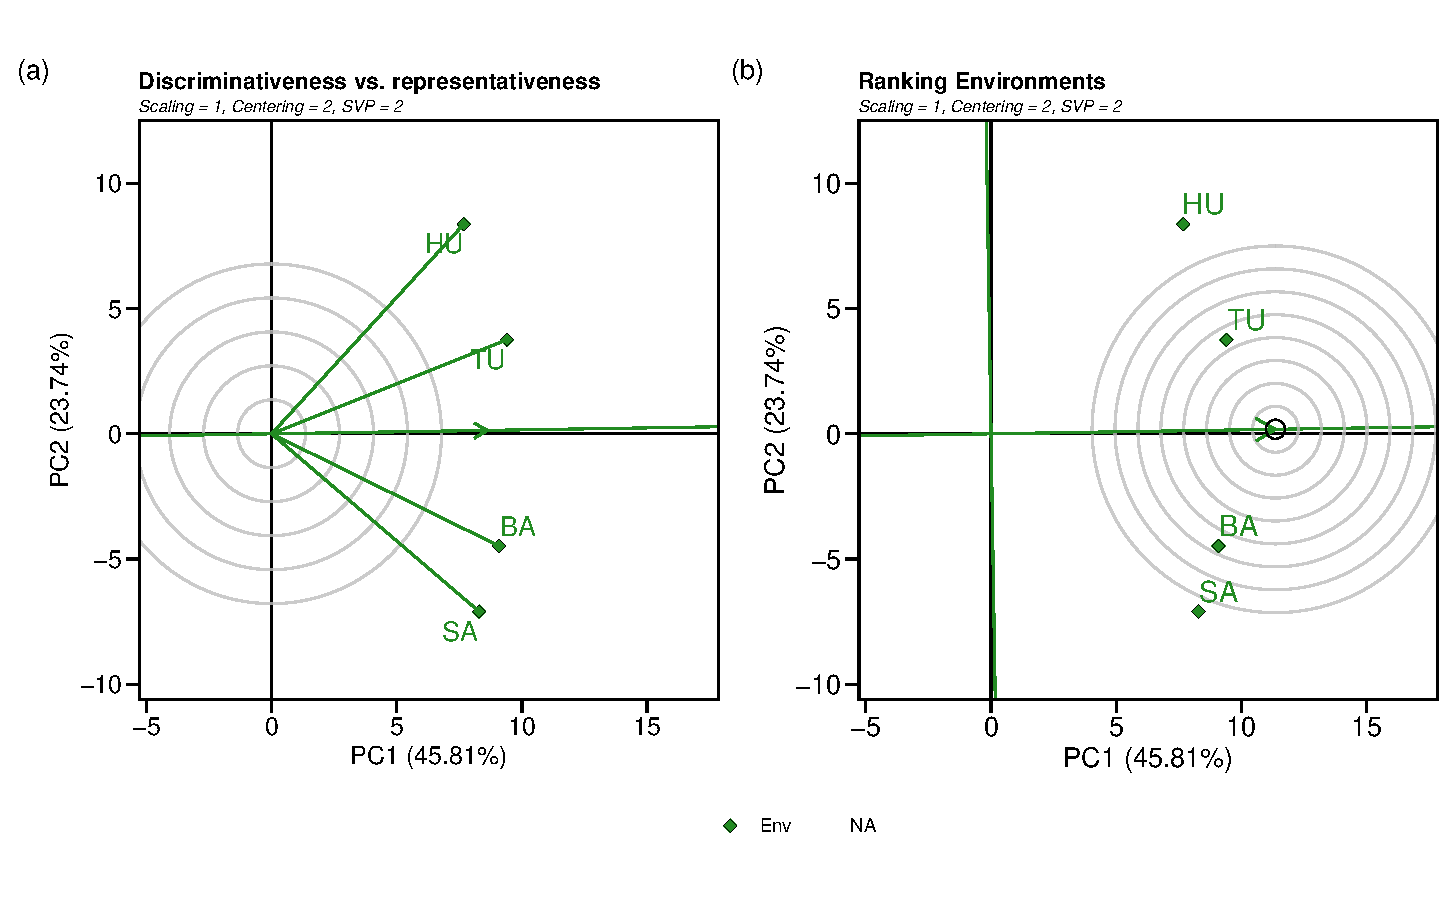
\includegraphics{figures/gge fig1-1} \end{center}

\hypertarget{biplot-type-3-which-won-where}{%
\paragraph{Biplot type 3:
Which-won-where}\label{biplot-type-3-which-won-where}}

GGE biplot done using:

\begin{itemize}
\tightlist
\item
  \textbf{sd}: each value is divided by the standard deviation of its
  corresponding environment.
\item
  \textbf{environment}: environment-centered (G+GE)
\item
  \textbf{genotype}: singular value is entirely partitioned into the
  environment eigenvectors, also called column metric preserving
\end{itemize}

\begin{Shaded}
\begin{Highlighting}[]
\NormalTok{gge\_model }\OtherTok{\textless{}{-}} \FunctionTok{gge}\NormalTok{(blues\_stage.I, loc, name, yield,}
                     \AttributeTok{centering =} \StringTok{"environment"}\NormalTok{, }\CommentTok{\#2}
                    \AttributeTok{scaling =} \StringTok{"sd"}\NormalTok{, }\CommentTok{\#1}
                    \AttributeTok{svp =} \StringTok{"genotype"}\NormalTok{)}\CommentTok{\#2)}

\NormalTok{e }\OtherTok{\textless{}{-}} \FunctionTok{plot}\NormalTok{(gge\_model, }\AttributeTok{type =} \DecValTok{3}\NormalTok{,}
          \AttributeTok{size.text.env =} \DecValTok{5}\NormalTok{,}
          \AttributeTok{plot\_theme =} \FunctionTok{theme\_metan}\NormalTok{(}\AttributeTok{grid =}  \StringTok{"both"}\NormalTok{,}\AttributeTok{color.background =} \FunctionTok{transparent\_color}\NormalTok{()),}
         \AttributeTok{axis\_expand =} \FloatTok{1.2}\NormalTok{,}
         \AttributeTok{size.line =} \FloatTok{0.7}\NormalTok{,}
         \AttributeTok{size.text.gen =} \DecValTok{4}\NormalTok{,}
         \AttributeTok{size.text.win =} \FloatTok{4.5}
         \CommentTok{\#title = F}
\NormalTok{        )}

\FunctionTok{print}\NormalTok{(e)}
\end{Highlighting}
\end{Shaded}

\begin{center}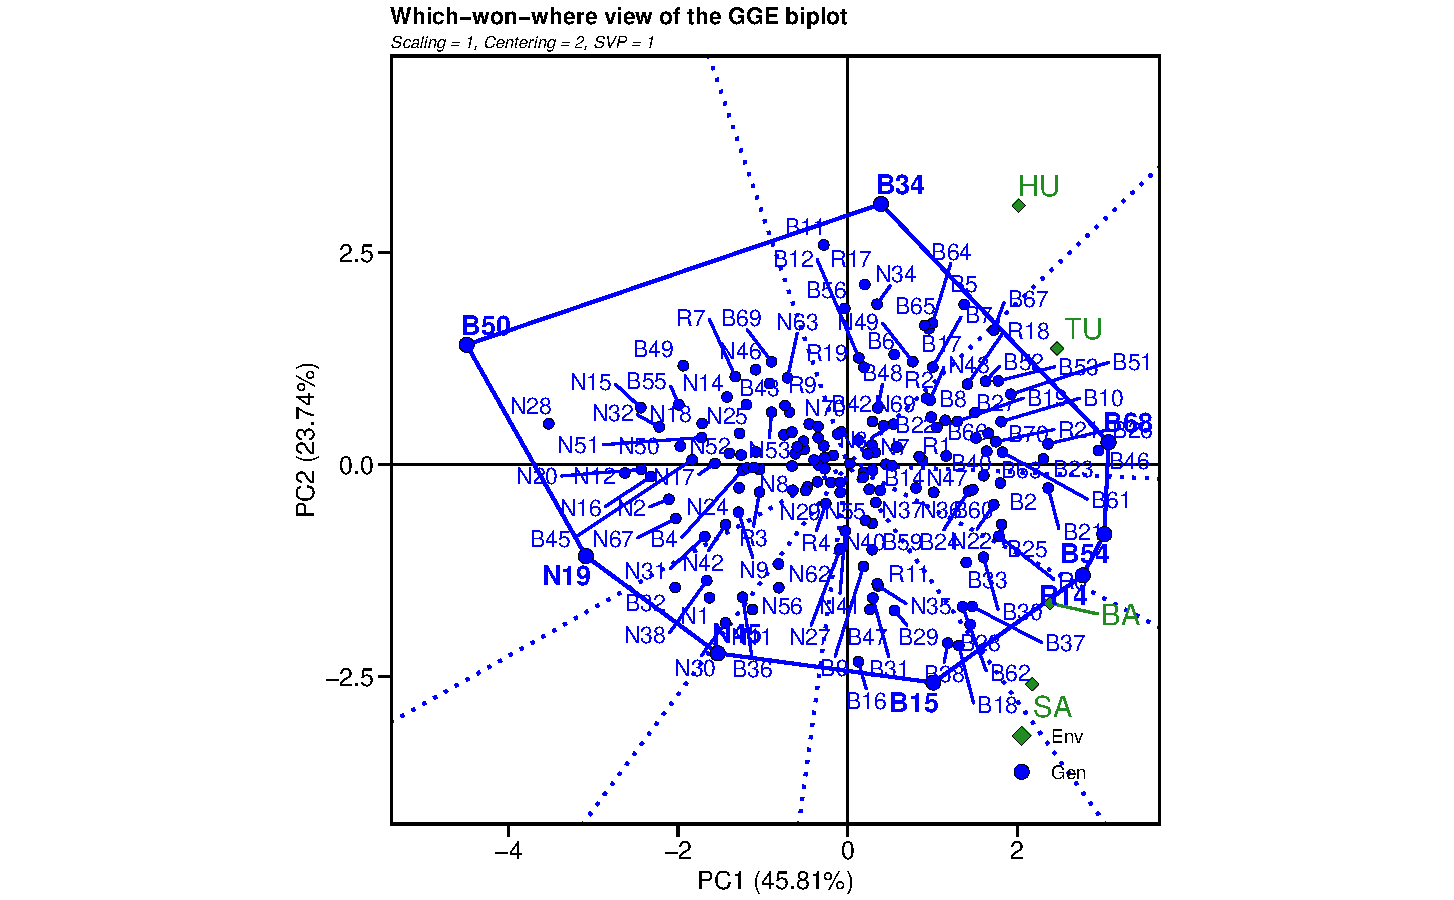
\includegraphics{figures/gge fig2-1} \end{center}

\hypertarget{mean-performance-and-stability-analysis}{%
\subsubsection{Mean performance and stability
analysis}\label{mean-performance-and-stability-analysis}}

WAASP index and BLUPs to estimate stability analysis.

\begin{Shaded}
\begin{Highlighting}[]
\CommentTok{\#blues\_stage.I\textless{}{-} na.omit(blues\_stage.I)}

\NormalTok{waasb\_model\_allMKT }\OtherTok{\textless{}{-}} 
  \FunctionTok{waasb}\NormalTok{(blues\_stage.I,}
        \AttributeTok{env =}\NormalTok{ loc,}
        \AttributeTok{gen =}\NormalTok{ name,}
        \AttributeTok{rep =}\NormalTok{ rep,}
        \AttributeTok{resp =}\NormalTok{ yield,}
        \AttributeTok{random =} \StringTok{"gen"}\NormalTok{, }\CommentTok{\#Default}
        \AttributeTok{verbose =} \ConstantTok{TRUE}\NormalTok{,}
        \AttributeTok{wresp =} \DecValTok{60}\NormalTok{) }\CommentTok{\#weight for response variable 60 and 40 for yielding and stability, respectively)}
\end{Highlighting}
\end{Shaded}

\begin{verbatim}
#> Evaluating trait yield |=================================================================================================================================================================================================| 100% 00:00:09 
#> ---------------------------------------------------------------------------
#> P-values for Likelihood Ratio Test of the analyzed traits
#> ---------------------------------------------------------------------------
#>     model    yield
#>  COMPLETE       NA
#>       GEN 1.18e-14
#>   GEN:ENV 1.51e-75
#> ---------------------------------------------------------------------------
#> All variables with significant (p < 0.05) genotype-vs-environment interaction
\end{verbatim}

\begin{Shaded}
\begin{Highlighting}[]
\NormalTok{waasb\_model}\OtherTok{\textless{}{-}}\NormalTok{ waasb\_model\_allMKT}\SpecialCharTok{$}\NormalTok{yield}\SpecialCharTok{$}\NormalTok{model}

\CommentTok{\#waasb\_ind \textless{}{-} gmd(waasb\_model, "WAASB")}
\CommentTok{\#print\_tbl(waasb\_ind)}

\CommentTok{\#desc \textless{}{-} c("Selected cultivar providing greater performance and stability for GY")}

\NormalTok{waasp\_plot }\OtherTok{\textless{}{-}} \FunctionTok{plot\_scores}\NormalTok{(waasb\_model\_allMKT, }\AttributeTok{type =} \DecValTok{3}\NormalTok{,}
          \AttributeTok{title =} \ConstantTok{FALSE}\NormalTok{,}
          \AttributeTok{size.tex.gen =} \DecValTok{4}\NormalTok{,}
          \AttributeTok{size.tex.env =} \DecValTok{4}\NormalTok{,}
          \AttributeTok{size.tex.lab =} \DecValTok{13}\NormalTok{,}
        \CommentTok{\# highlight = c("B55", "B1" , "B29", "B20" ,"B28"),}
         \AttributeTok{plot\_theme =} \FunctionTok{theme\_metan}\NormalTok{(}\AttributeTok{grid =}  \StringTok{"both"}\NormalTok{,}\AttributeTok{color.background =} \FunctionTok{transparent\_color}\NormalTok{())}
\NormalTok{        ) }\SpecialCharTok{+}
  
  \FunctionTok{geom\_mark\_rect}\NormalTok{(}\FunctionTok{aes}\NormalTok{(}\AttributeTok{filter =}\NormalTok{  Code  }\SpecialCharTok{\%in\%} \FunctionTok{c}\NormalTok{(}\StringTok{"N64"}\NormalTok{, }\StringTok{"N40"}\NormalTok{, }\StringTok{"B68"}\NormalTok{, }\StringTok{"N7"}\NormalTok{),}
\NormalTok{                     ),}
               \AttributeTok{label.fontsize =} \DecValTok{10}\NormalTok{,}
               \AttributeTok{show.legend =}\NormalTok{ F,}
               \AttributeTok{con.cap =} \DecValTok{0}\NormalTok{,}
               \AttributeTok{con.colour =} \StringTok{"red"}\NormalTok{,}
               \AttributeTok{color =} \StringTok{"red"}\NormalTok{,}
               \AttributeTok{expand =} \FloatTok{0.01}\NormalTok{,}
               \AttributeTok{label.buffer =} \FunctionTok{unit}\NormalTok{(}\DecValTok{10}\NormalTok{, }\StringTok{"cm"}\NormalTok{))}\SpecialCharTok{+}
\CommentTok{\#theme\_gray()+}
\FunctionTok{theme}\NormalTok{(}\AttributeTok{legend.position =} \FunctionTok{c}\NormalTok{(}\FloatTok{0.1}\NormalTok{, }\FloatTok{0.9}\NormalTok{),}
      \AttributeTok{legend.background =} \FunctionTok{element\_blank}\NormalTok{(),}
      \AttributeTok{legend.title =} \FunctionTok{element\_blank}\NormalTok{(),}
      \AttributeTok{aspect.ratio =} \DecValTok{1}\NormalTok{) }\SpecialCharTok{+}
  \FunctionTok{labs}\NormalTok{(}\AttributeTok{x =} \StringTok{"GY"}\NormalTok{) }

\FunctionTok{print}\NormalTok{(waasp\_plot)}
\end{Highlighting}
\end{Shaded}

\begin{center}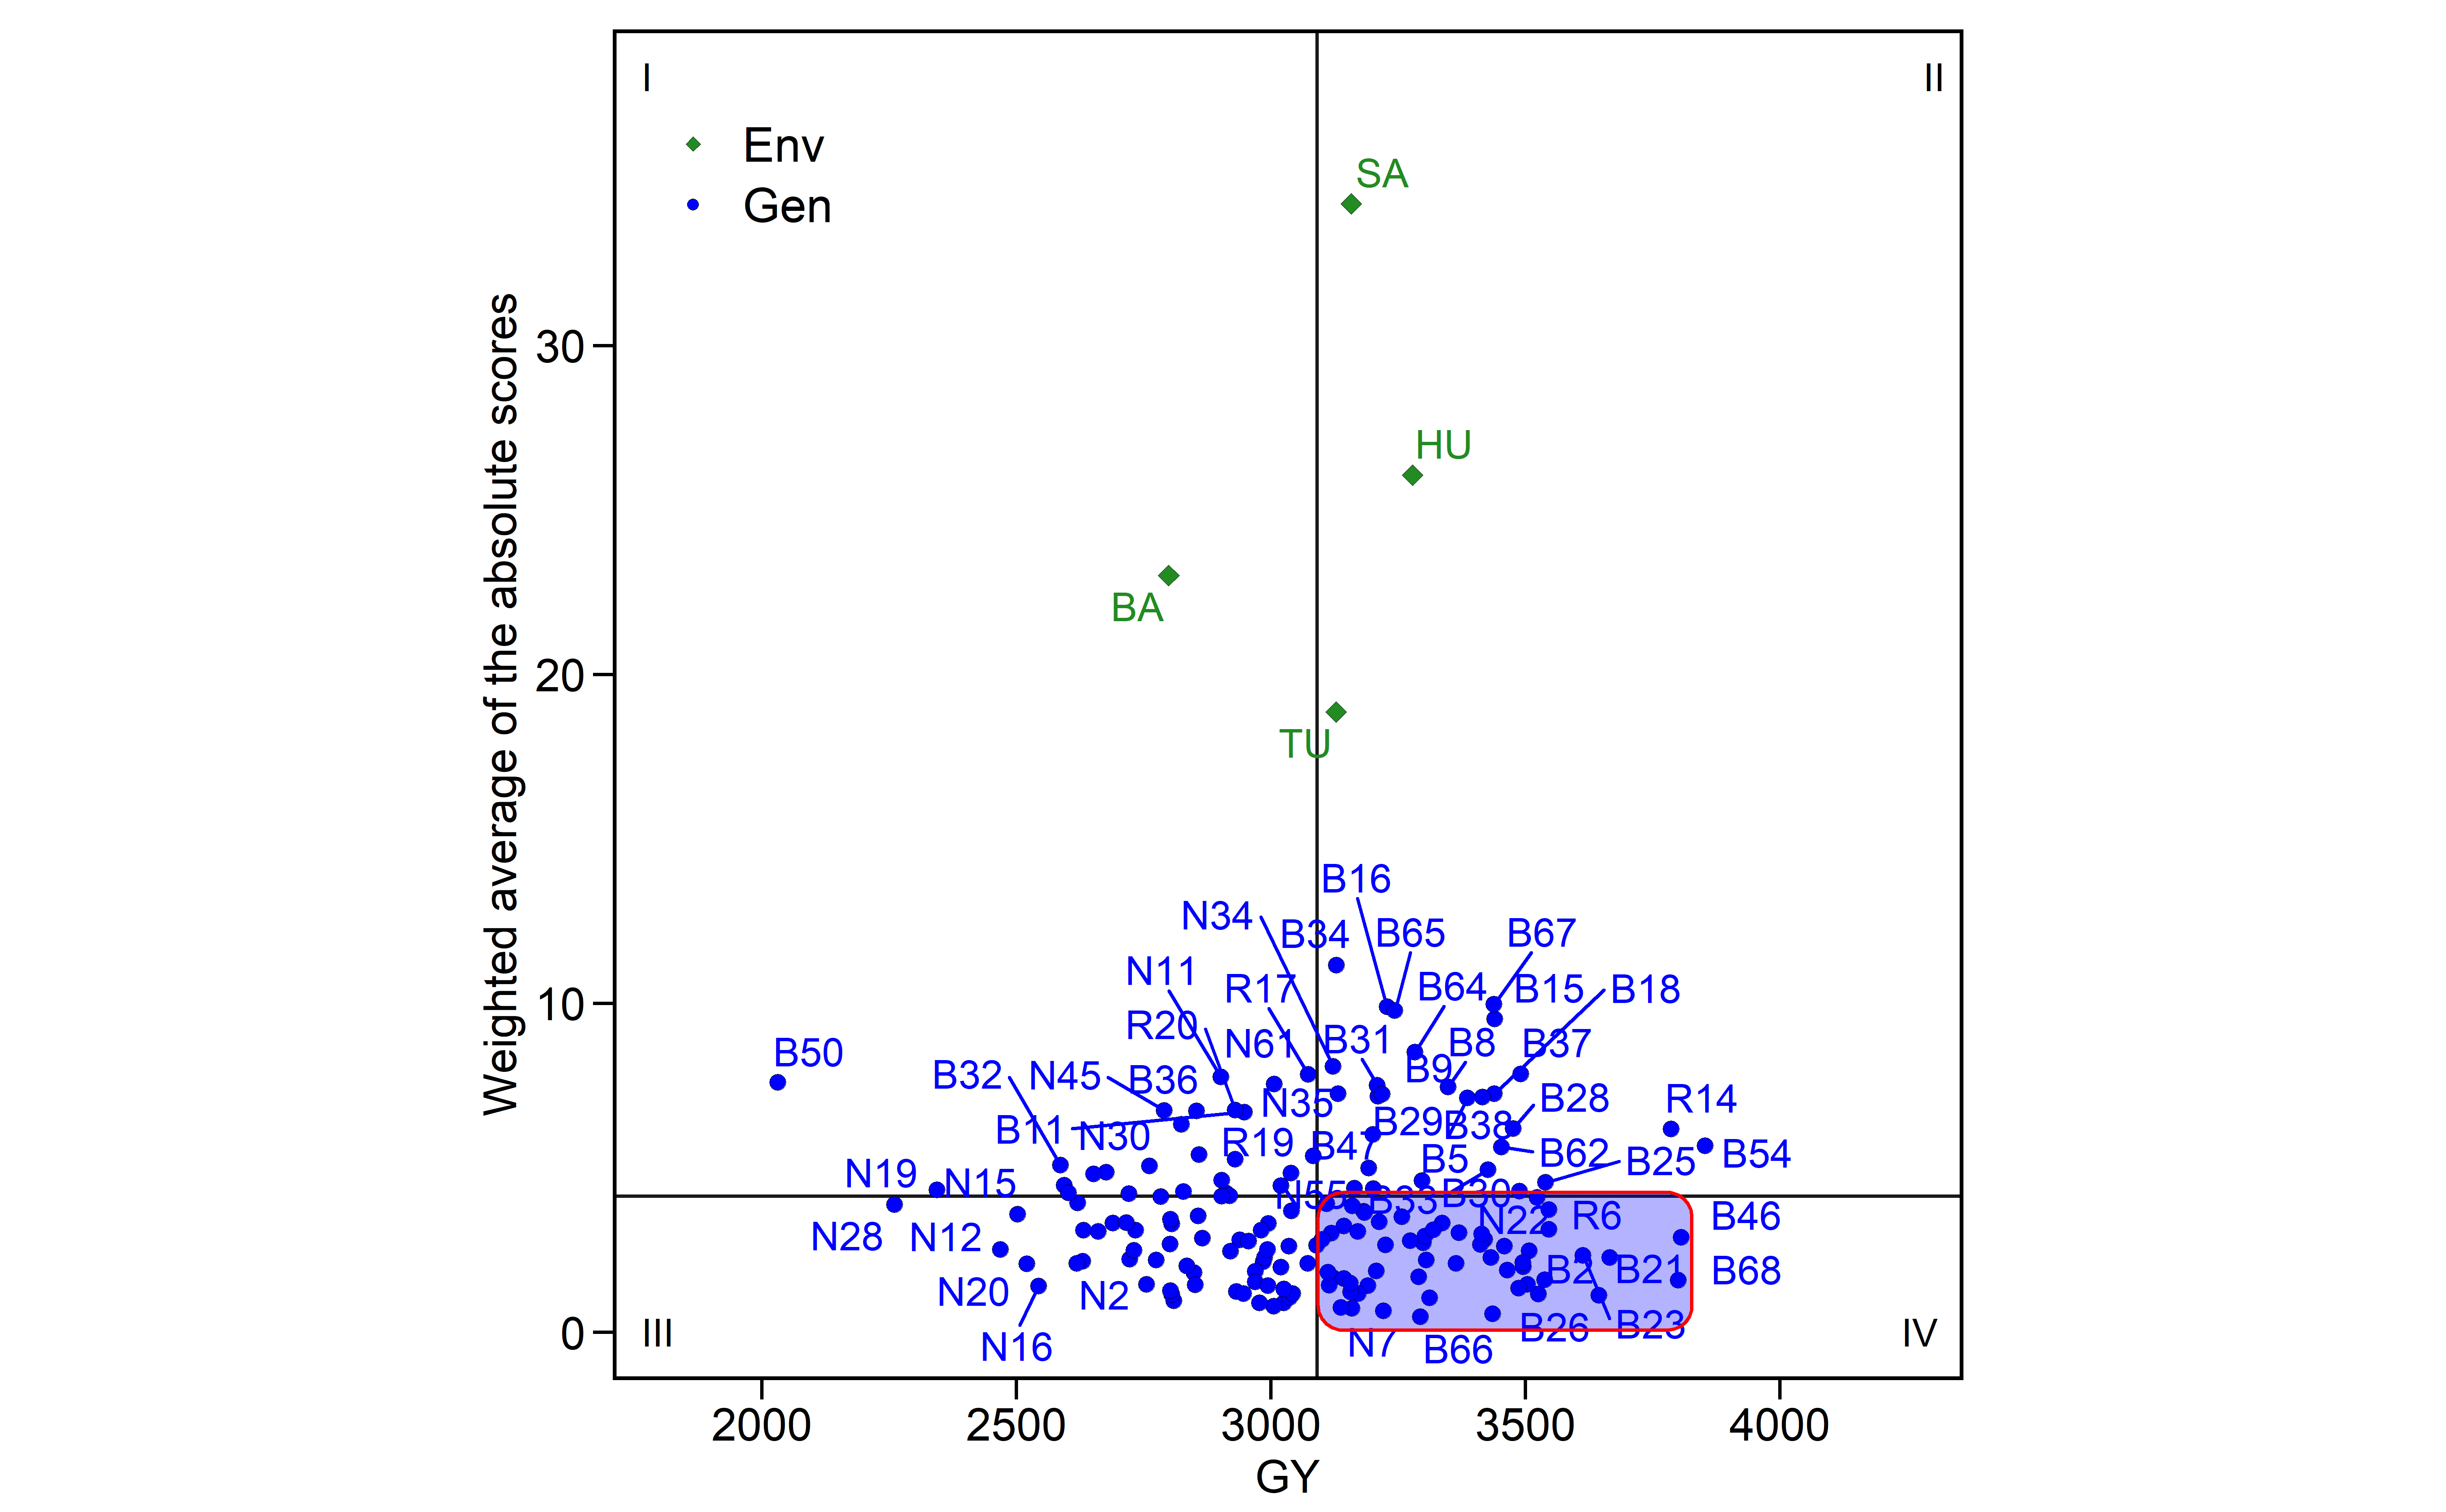
\includegraphics{figures/mod metan stab-1} \end{center}

\begin{Shaded}
\begin{Highlighting}[]
\NormalTok{waasb\_model\_meanWaasb}\OtherTok{\textless{}{-}}\FunctionTok{mean}\NormalTok{(waasb\_model}\SpecialCharTok{$}\NormalTok{WAASB)}
\NormalTok{waasb\_model\_meanY}\OtherTok{\textless{}{-}}\FunctionTok{mean}\NormalTok{(waasb\_model}\SpecialCharTok{$}\NormalTok{Y)}

\NormalTok{selected }\OtherTok{\textless{}{-}}\NormalTok{ waasb\_model }\SpecialCharTok{\%\textgreater{}\%}
\NormalTok{  dplyr}\SpecialCharTok{::}\FunctionTok{filter}\NormalTok{(Y }\SpecialCharTok{\textgreater{}=}\NormalTok{ waasb\_model\_meanY }\SpecialCharTok{\&}\NormalTok{ WAASB }\SpecialCharTok{\textless{}=}\NormalTok{ waasb\_model\_meanWaasb) }

\NormalTok{selected\_table }\OtherTok{\textless{}{-}}\NormalTok{ selected}

\ControlFlowTok{if}\NormalTok{ (knitr}\SpecialCharTok{::}\FunctionTok{is\_html\_output}\NormalTok{()) \{}

  \FunctionTok{print\_table}\NormalTok{(selected\_table)}
  
\NormalTok{\}}\ControlFlowTok{else}\NormalTok{\{}
  
\NormalTok{ selected\_table[,}\DecValTok{1}\SpecialCharTok{:}\DecValTok{8}\NormalTok{] }
\NormalTok{\}}
\end{Highlighting}
\end{Shaded}

\global\setlength{\Oldarrayrulewidth}{\arrayrulewidth}

\global\setlength{\Oldtabcolsep}{\tabcolsep}

\setlength{\tabcolsep}{0pt}

\renewcommand*{\arraystretch}{1.5}



\providecommand{\ascline}[3]{\noalign{\global\arrayrulewidth #1}\arrayrulecolor[HTML]{#2}\cline{#3}}

\begin{longtable}[c]{|p{0.77in}|p{0.77in}|p{0.75in}|p{0.75in}|p{0.75in}|p{0.75in}|p{0.75in}|p{0.75in}}



\ascline{1.5pt}{666666}{1-8}

\multicolumn{1}{>{\raggedright}m{\dimexpr 0.77in+0\tabcolsep}}{\textcolor[HTML]{000000}{\fontsize{9}{9}\selectfont{\global\setmainfont{Arial}{\textbf{type}}}}} & \multicolumn{1}{>{\raggedright}m{\dimexpr 0.77in+0\tabcolsep}}{\textcolor[HTML]{000000}{\fontsize{9}{9}\selectfont{\global\setmainfont{Arial}{\textbf{Code}}}}} & \multicolumn{1}{>{\raggedleft}m{\dimexpr 0.75in+0\tabcolsep}}{\textcolor[HTML]{000000}{\fontsize{9}{9}\selectfont{\global\setmainfont{Arial}{\textbf{Y}}}}} & \multicolumn{1}{>{\raggedleft}m{\dimexpr 0.75in+0\tabcolsep}}{\textcolor[HTML]{000000}{\fontsize{9}{9}\selectfont{\global\setmainfont{Arial}{\textbf{PC1}}}}} & \multicolumn{1}{>{\raggedleft}m{\dimexpr 0.75in+0\tabcolsep}}{\textcolor[HTML]{000000}{\fontsize{9}{9}\selectfont{\global\setmainfont{Arial}{\textbf{PC2}}}}} & \multicolumn{1}{>{\raggedleft}m{\dimexpr 0.75in+0\tabcolsep}}{\textcolor[HTML]{000000}{\fontsize{9}{9}\selectfont{\global\setmainfont{Arial}{\textbf{PC3}}}}} & \multicolumn{1}{>{\raggedleft}m{\dimexpr 0.75in+0\tabcolsep}}{\textcolor[HTML]{000000}{\fontsize{9}{9}\selectfont{\global\setmainfont{Arial}{\textbf{WAASB}}}}} & \multicolumn{1}{>{\raggedleft}m{\dimexpr 0.75in+0\tabcolsep}}{\textcolor[HTML]{000000}{\fontsize{9}{9}\selectfont{\global\setmainfont{Arial}{\textbf{PctResp}}}}} \\

\ascline{0.75pt}{666666}{1-8}



\multicolumn{1}{>{\raggedright}m{\dimexpr 0.77in+0\tabcolsep}}{\textcolor[HTML]{999999}{\fontsize{9}{9}\selectfont{\global\setmainfont{Arial}{\textbf{character}}}}} & \multicolumn{1}{>{\raggedright}m{\dimexpr 0.77in+0\tabcolsep}}{\textcolor[HTML]{999999}{\fontsize{9}{9}\selectfont{\global\setmainfont{Arial}{\textbf{character}}}}} & \multicolumn{1}{>{\raggedleft}m{\dimexpr 0.75in+0\tabcolsep}}{\textcolor[HTML]{999999}{\fontsize{9}{9}\selectfont{\global\setmainfont{Arial}{\textbf{numeric}}}}} & \multicolumn{1}{>{\raggedleft}m{\dimexpr 0.75in+0\tabcolsep}}{\textcolor[HTML]{999999}{\fontsize{9}{9}\selectfont{\global\setmainfont{Arial}{\textbf{numeric}}}}} & \multicolumn{1}{>{\raggedleft}m{\dimexpr 0.75in+0\tabcolsep}}{\textcolor[HTML]{999999}{\fontsize{9}{9}\selectfont{\global\setmainfont{Arial}{\textbf{numeric}}}}} & \multicolumn{1}{>{\raggedleft}m{\dimexpr 0.75in+0\tabcolsep}}{\textcolor[HTML]{999999}{\fontsize{9}{9}\selectfont{\global\setmainfont{Arial}{\textbf{numeric}}}}} & \multicolumn{1}{>{\raggedleft}m{\dimexpr 0.75in+0\tabcolsep}}{\textcolor[HTML]{999999}{\fontsize{9}{9}\selectfont{\global\setmainfont{Arial}{\textbf{numeric}}}}} & \multicolumn{1}{>{\raggedleft}m{\dimexpr 0.75in+0\tabcolsep}}{\textcolor[HTML]{999999}{\fontsize{9}{9}\selectfont{\global\setmainfont{Arial}{\textbf{numeric}}}}} \\

\ascline{1.5pt}{666666}{1-8}\endfirsthead

\ascline{1.5pt}{666666}{1-8}

\multicolumn{1}{>{\raggedright}m{\dimexpr 0.77in+0\tabcolsep}}{\textcolor[HTML]{000000}{\fontsize{9}{9}\selectfont{\global\setmainfont{Arial}{\textbf{type}}}}} & \multicolumn{1}{>{\raggedright}m{\dimexpr 0.77in+0\tabcolsep}}{\textcolor[HTML]{000000}{\fontsize{9}{9}\selectfont{\global\setmainfont{Arial}{\textbf{Code}}}}} & \multicolumn{1}{>{\raggedleft}m{\dimexpr 0.75in+0\tabcolsep}}{\textcolor[HTML]{000000}{\fontsize{9}{9}\selectfont{\global\setmainfont{Arial}{\textbf{Y}}}}} & \multicolumn{1}{>{\raggedleft}m{\dimexpr 0.75in+0\tabcolsep}}{\textcolor[HTML]{000000}{\fontsize{9}{9}\selectfont{\global\setmainfont{Arial}{\textbf{PC1}}}}} & \multicolumn{1}{>{\raggedleft}m{\dimexpr 0.75in+0\tabcolsep}}{\textcolor[HTML]{000000}{\fontsize{9}{9}\selectfont{\global\setmainfont{Arial}{\textbf{PC2}}}}} & \multicolumn{1}{>{\raggedleft}m{\dimexpr 0.75in+0\tabcolsep}}{\textcolor[HTML]{000000}{\fontsize{9}{9}\selectfont{\global\setmainfont{Arial}{\textbf{PC3}}}}} & \multicolumn{1}{>{\raggedleft}m{\dimexpr 0.75in+0\tabcolsep}}{\textcolor[HTML]{000000}{\fontsize{9}{9}\selectfont{\global\setmainfont{Arial}{\textbf{WAASB}}}}} & \multicolumn{1}{>{\raggedleft}m{\dimexpr 0.75in+0\tabcolsep}}{\textcolor[HTML]{000000}{\fontsize{9}{9}\selectfont{\global\setmainfont{Arial}{\textbf{PctResp}}}}} \\

\ascline{0.75pt}{666666}{1-8}



\multicolumn{1}{>{\raggedright}m{\dimexpr 0.77in+0\tabcolsep}}{\textcolor[HTML]{999999}{\fontsize{9}{9}\selectfont{\global\setmainfont{Arial}{\textbf{character}}}}} & \multicolumn{1}{>{\raggedright}m{\dimexpr 0.77in+0\tabcolsep}}{\textcolor[HTML]{999999}{\fontsize{9}{9}\selectfont{\global\setmainfont{Arial}{\textbf{character}}}}} & \multicolumn{1}{>{\raggedleft}m{\dimexpr 0.75in+0\tabcolsep}}{\textcolor[HTML]{999999}{\fontsize{9}{9}\selectfont{\global\setmainfont{Arial}{\textbf{numeric}}}}} & \multicolumn{1}{>{\raggedleft}m{\dimexpr 0.75in+0\tabcolsep}}{\textcolor[HTML]{999999}{\fontsize{9}{9}\selectfont{\global\setmainfont{Arial}{\textbf{numeric}}}}} & \multicolumn{1}{>{\raggedleft}m{\dimexpr 0.75in+0\tabcolsep}}{\textcolor[HTML]{999999}{\fontsize{9}{9}\selectfont{\global\setmainfont{Arial}{\textbf{numeric}}}}} & \multicolumn{1}{>{\raggedleft}m{\dimexpr 0.75in+0\tabcolsep}}{\textcolor[HTML]{999999}{\fontsize{9}{9}\selectfont{\global\setmainfont{Arial}{\textbf{numeric}}}}} & \multicolumn{1}{>{\raggedleft}m{\dimexpr 0.75in+0\tabcolsep}}{\textcolor[HTML]{999999}{\fontsize{9}{9}\selectfont{\global\setmainfont{Arial}{\textbf{numeric}}}}} & \multicolumn{1}{>{\raggedleft}m{\dimexpr 0.75in+0\tabcolsep}}{\textcolor[HTML]{999999}{\fontsize{9}{9}\selectfont{\global\setmainfont{Arial}{\textbf{numeric}}}}} \\

\ascline{1.5pt}{666666}{1-8}\endhead



\multicolumn{8}{>{\raggedright}m{\dimexpr 6.05in+14\tabcolsep}}{\textcolor[HTML]{000000}{\fontsize{9}{9}\selectfont{\global\setmainfont{Arial}{n:\ 56}}}} \\

\ascline{0.75pt}{666666}{1-8}\endfoot



\multicolumn{1}{>{\raggedright}m{\dimexpr 0.77in+0\tabcolsep}}{\textcolor[HTML]{000000}{\fontsize{9}{9}\selectfont{\global\setmainfont{Arial}{GEN}}}} & \multicolumn{1}{>{\raggedright}m{\dimexpr 0.77in+0\tabcolsep}}{\textcolor[HTML]{000000}{\fontsize{9}{9}\selectfont{\global\setmainfont{Arial}{B10}}}} & \multicolumn{1}{>{\raggedleft}m{\dimexpr 0.75in+0\tabcolsep}}{\textcolor[HTML]{000000}{\fontsize{9}{9}\selectfont{\global\setmainfont{Arial}{3,525.7}}}} & \multicolumn{1}{>{\raggedleft}m{\dimexpr 0.75in+0\tabcolsep}}{\textcolor[HTML]{000000}{\fontsize{9}{9}\selectfont{\global\setmainfont{Arial}{0.1}}}} & \multicolumn{1}{>{\raggedleft}m{\dimexpr 0.75in+0\tabcolsep}}{\textcolor[HTML]{000000}{\fontsize{9}{9}\selectfont{\global\setmainfont{Arial}{1.4}}}} & \multicolumn{1}{>{\raggedleft}m{\dimexpr 0.75in+0\tabcolsep}}{\textcolor[HTML]{000000}{\fontsize{9}{9}\selectfont{\global\setmainfont{Arial}{-3.2}}}} & \multicolumn{1}{>{\raggedleft}m{\dimexpr 0.75in+0\tabcolsep}}{\textcolor[HTML]{000000}{\fontsize{9}{9}\selectfont{\global\setmainfont{Arial}{1.2}}}} & \multicolumn{1}{>{\raggedleft}m{\dimexpr 0.75in+0\tabcolsep}}{\textcolor[HTML]{000000}{\fontsize{9}{9}\selectfont{\global\setmainfont{Arial}{82.0}}}} \\

\ascline{0.75pt}{666666}{1-8}



\multicolumn{1}{>{\raggedright}m{\dimexpr 0.77in+0\tabcolsep}}{\textcolor[HTML]{000000}{\fontsize{9}{9}\selectfont{\global\setmainfont{Arial}{GEN}}}} & \multicolumn{1}{>{\raggedright}m{\dimexpr 0.77in+0\tabcolsep}}{\textcolor[HTML]{000000}{\fontsize{9}{9}\selectfont{\global\setmainfont{Arial}{B13}}}} & \multicolumn{1}{>{\raggedleft}m{\dimexpr 0.75in+0\tabcolsep}}{\textcolor[HTML]{000000}{\fontsize{9}{9}\selectfont{\global\setmainfont{Arial}{3,122.0}}}} & \multicolumn{1}{>{\raggedleft}m{\dimexpr 0.75in+0\tabcolsep}}{\textcolor[HTML]{000000}{\fontsize{9}{9}\selectfont{\global\setmainfont{Arial}{0.7}}}} & \multicolumn{1}{>{\raggedleft}m{\dimexpr 0.75in+0\tabcolsep}}{\textcolor[HTML]{000000}{\fontsize{9}{9}\selectfont{\global\setmainfont{Arial}{1.2}}}} & \multicolumn{1}{>{\raggedleft}m{\dimexpr 0.75in+0\tabcolsep}}{\textcolor[HTML]{000000}{\fontsize{9}{9}\selectfont{\global\setmainfont{Arial}{4.5}}}} & \multicolumn{1}{>{\raggedleft}m{\dimexpr 0.75in+0\tabcolsep}}{\textcolor[HTML]{000000}{\fontsize{9}{9}\selectfont{\global\setmainfont{Arial}{1.7}}}} & \multicolumn{1}{>{\raggedleft}m{\dimexpr 0.75in+0\tabcolsep}}{\textcolor[HTML]{000000}{\fontsize{9}{9}\selectfont{\global\setmainfont{Arial}{59.9}}}} \\

\ascline{0.75pt}{666666}{1-8}



\multicolumn{1}{>{\raggedright}m{\dimexpr 0.77in+0\tabcolsep}}{\textcolor[HTML]{000000}{\fontsize{9}{9}\selectfont{\global\setmainfont{Arial}{GEN}}}} & \multicolumn{1}{>{\raggedright}m{\dimexpr 0.77in+0\tabcolsep}}{\textcolor[HTML]{000000}{\fontsize{9}{9}\selectfont{\global\setmainfont{Arial}{B14}}}} & \multicolumn{1}{>{\raggedleft}m{\dimexpr 0.75in+0\tabcolsep}}{\textcolor[HTML]{000000}{\fontsize{9}{9}\selectfont{\global\setmainfont{Arial}{3,299.5}}}} & \multicolumn{1}{>{\raggedleft}m{\dimexpr 0.75in+0\tabcolsep}}{\textcolor[HTML]{000000}{\fontsize{9}{9}\selectfont{\global\setmainfont{Arial}{1.8}}}} & \multicolumn{1}{>{\raggedleft}m{\dimexpr 0.75in+0\tabcolsep}}{\textcolor[HTML]{000000}{\fontsize{9}{9}\selectfont{\global\setmainfont{Arial}{-2.9}}}} & \multicolumn{1}{>{\raggedleft}m{\dimexpr 0.75in+0\tabcolsep}}{\textcolor[HTML]{000000}{\fontsize{9}{9}\selectfont{\global\setmainfont{Arial}{-4.5}}}} & \multicolumn{1}{>{\raggedleft}m{\dimexpr 0.75in+0\tabcolsep}}{\textcolor[HTML]{000000}{\fontsize{9}{9}\selectfont{\global\setmainfont{Arial}{2.7}}}} & \multicolumn{1}{>{\raggedleft}m{\dimexpr 0.75in+0\tabcolsep}}{\textcolor[HTML]{000000}{\fontsize{9}{9}\selectfont{\global\setmainfont{Arial}{69.6}}}} \\

\ascline{0.75pt}{666666}{1-8}



\multicolumn{1}{>{\raggedright}m{\dimexpr 0.77in+0\tabcolsep}}{\textcolor[HTML]{000000}{\fontsize{9}{9}\selectfont{\global\setmainfont{Arial}{GEN}}}} & \multicolumn{1}{>{\raggedright}m{\dimexpr 0.77in+0\tabcolsep}}{\textcolor[HTML]{000000}{\fontsize{9}{9}\selectfont{\global\setmainfont{Arial}{B19}}}} & \multicolumn{1}{>{\raggedleft}m{\dimexpr 0.75in+0\tabcolsep}}{\textcolor[HTML]{000000}{\fontsize{9}{9}\selectfont{\global\setmainfont{Arial}{3,369.1}}}} & \multicolumn{1}{>{\raggedleft}m{\dimexpr 0.75in+0\tabcolsep}}{\textcolor[HTML]{000000}{\fontsize{9}{9}\selectfont{\global\setmainfont{Arial}{-0.4}}}} & \multicolumn{1}{>{\raggedleft}m{\dimexpr 0.75in+0\tabcolsep}}{\textcolor[HTML]{000000}{\fontsize{9}{9}\selectfont{\global\setmainfont{Arial}{4.3}}}} & \multicolumn{1}{>{\raggedleft}m{\dimexpr 0.75in+0\tabcolsep}}{\textcolor[HTML]{000000}{\fontsize{9}{9}\selectfont{\global\setmainfont{Arial}{6.9}}}} & \multicolumn{1}{>{\raggedleft}m{\dimexpr 0.75in+0\tabcolsep}}{\textcolor[HTML]{000000}{\fontsize{9}{9}\selectfont{\global\setmainfont{Arial}{3.0}}}} & \multicolumn{1}{>{\raggedleft}m{\dimexpr 0.75in+0\tabcolsep}}{\textcolor[HTML]{000000}{\fontsize{9}{9}\selectfont{\global\setmainfont{Arial}{73.4}}}} \\

\ascline{0.75pt}{666666}{1-8}



\multicolumn{1}{>{\raggedright}m{\dimexpr 0.77in+0\tabcolsep}}{\textcolor[HTML]{000000}{\fontsize{9}{9}\selectfont{\global\setmainfont{Arial}{GEN}}}} & \multicolumn{1}{>{\raggedright}m{\dimexpr 0.77in+0\tabcolsep}}{\textcolor[HTML]{000000}{\fontsize{9}{9}\selectfont{\global\setmainfont{Arial}{B2}}}} & \multicolumn{1}{>{\raggedleft}m{\dimexpr 0.75in+0\tabcolsep}}{\textcolor[HTML]{000000}{\fontsize{9}{9}\selectfont{\global\setmainfont{Arial}{3,545.5}}}} & \multicolumn{1}{>{\raggedleft}m{\dimexpr 0.75in+0\tabcolsep}}{\textcolor[HTML]{000000}{\fontsize{9}{9}\selectfont{\global\setmainfont{Arial}{4.1}}}} & \multicolumn{1}{>{\raggedleft}m{\dimexpr 0.75in+0\tabcolsep}}{\textcolor[HTML]{000000}{\fontsize{9}{9}\selectfont{\global\setmainfont{Arial}{1.2}}}} & \multicolumn{1}{>{\raggedleft}m{\dimexpr 0.75in+0\tabcolsep}}{\textcolor[HTML]{000000}{\fontsize{9}{9}\selectfont{\global\setmainfont{Arial}{-3.8}}}} & \multicolumn{1}{>{\raggedleft}m{\dimexpr 0.75in+0\tabcolsep}}{\textcolor[HTML]{000000}{\fontsize{9}{9}\selectfont{\global\setmainfont{Arial}{3.1}}}} & \multicolumn{1}{>{\raggedleft}m{\dimexpr 0.75in+0\tabcolsep}}{\textcolor[HTML]{000000}{\fontsize{9}{9}\selectfont{\global\setmainfont{Arial}{83.1}}}} \\

\ascline{0.75pt}{666666}{1-8}



\multicolumn{1}{>{\raggedright}m{\dimexpr 0.77in+0\tabcolsep}}{\textcolor[HTML]{000000}{\fontsize{9}{9}\selectfont{\global\setmainfont{Arial}{GEN}}}} & \multicolumn{1}{>{\raggedright}m{\dimexpr 0.77in+0\tabcolsep}}{\textcolor[HTML]{000000}{\fontsize{9}{9}\selectfont{\global\setmainfont{Arial}{B21}}}} & \multicolumn{1}{>{\raggedleft}m{\dimexpr 0.75in+0\tabcolsep}}{\textcolor[HTML]{000000}{\fontsize{9}{9}\selectfont{\global\setmainfont{Arial}{3,665.5}}}} & \multicolumn{1}{>{\raggedleft}m{\dimexpr 0.75in+0\tabcolsep}}{\textcolor[HTML]{000000}{\fontsize{9}{9}\selectfont{\global\setmainfont{Arial}{4.2}}}} & \multicolumn{1}{>{\raggedleft}m{\dimexpr 0.75in+0\tabcolsep}}{\textcolor[HTML]{000000}{\fontsize{9}{9}\selectfont{\global\setmainfont{Arial}{-0.2}}}} & \multicolumn{1}{>{\raggedleft}m{\dimexpr 0.75in+0\tabcolsep}}{\textcolor[HTML]{000000}{\fontsize{9}{9}\selectfont{\global\setmainfont{Arial}{-1.0}}}} & \multicolumn{1}{>{\raggedleft}m{\dimexpr 0.75in+0\tabcolsep}}{\textcolor[HTML]{000000}{\fontsize{9}{9}\selectfont{\global\setmainfont{Arial}{2.3}}}} & \multicolumn{1}{>{\raggedleft}m{\dimexpr 0.75in+0\tabcolsep}}{\textcolor[HTML]{000000}{\fontsize{9}{9}\selectfont{\global\setmainfont{Arial}{89.7}}}} \\

\ascline{0.75pt}{666666}{1-8}



\multicolumn{1}{>{\raggedright}m{\dimexpr 0.77in+0\tabcolsep}}{\textcolor[HTML]{000000}{\fontsize{9}{9}\selectfont{\global\setmainfont{Arial}{GEN}}}} & \multicolumn{1}{>{\raggedright}m{\dimexpr 0.77in+0\tabcolsep}}{\textcolor[HTML]{000000}{\fontsize{9}{9}\selectfont{\global\setmainfont{Arial}{B22}}}} & \multicolumn{1}{>{\raggedleft}m{\dimexpr 0.75in+0\tabcolsep}}{\textcolor[HTML]{000000}{\fontsize{9}{9}\selectfont{\global\setmainfont{Arial}{3,305.2}}}} & \multicolumn{1}{>{\raggedleft}m{\dimexpr 0.75in+0\tabcolsep}}{\textcolor[HTML]{000000}{\fontsize{9}{9}\selectfont{\global\setmainfont{Arial}{-2.0}}}} & \multicolumn{1}{>{\raggedleft}m{\dimexpr 0.75in+0\tabcolsep}}{\textcolor[HTML]{000000}{\fontsize{9}{9}\selectfont{\global\setmainfont{Arial}{-0.4}}}} & \multicolumn{1}{>{\raggedleft}m{\dimexpr 0.75in+0\tabcolsep}}{\textcolor[HTML]{000000}{\fontsize{9}{9}\selectfont{\global\setmainfont{Arial}{5.4}}}} & \multicolumn{1}{>{\raggedleft}m{\dimexpr 0.75in+0\tabcolsep}}{\textcolor[HTML]{000000}{\fontsize{9}{9}\selectfont{\global\setmainfont{Arial}{2.2}}}} & \multicolumn{1}{>{\raggedleft}m{\dimexpr 0.75in+0\tabcolsep}}{\textcolor[HTML]{000000}{\fontsize{9}{9}\selectfont{\global\setmainfont{Arial}{69.9}}}} \\

\ascline{0.75pt}{666666}{1-8}



\multicolumn{1}{>{\raggedright}m{\dimexpr 0.77in+0\tabcolsep}}{\textcolor[HTML]{000000}{\fontsize{9}{9}\selectfont{\global\setmainfont{Arial}{GEN}}}} & \multicolumn{1}{>{\raggedright}m{\dimexpr 0.77in+0\tabcolsep}}{\textcolor[HTML]{000000}{\fontsize{9}{9}\selectfont{\global\setmainfont{Arial}{B23}}}} & \multicolumn{1}{>{\raggedleft}m{\dimexpr 0.75in+0\tabcolsep}}{\textcolor[HTML]{000000}{\fontsize{9}{9}\selectfont{\global\setmainfont{Arial}{3,612.8}}}} & \multicolumn{1}{>{\raggedleft}m{\dimexpr 0.75in+0\tabcolsep}}{\textcolor[HTML]{000000}{\fontsize{9}{9}\selectfont{\global\setmainfont{Arial}{-0.3}}}} & \multicolumn{1}{>{\raggedleft}m{\dimexpr 0.75in+0\tabcolsep}}{\textcolor[HTML]{000000}{\fontsize{9}{9}\selectfont{\global\setmainfont{Arial}{-5.8}}}} & \multicolumn{1}{>{\raggedleft}m{\dimexpr 0.75in+0\tabcolsep}}{\textcolor[HTML]{000000}{\fontsize{9}{9}\selectfont{\global\setmainfont{Arial}{1.7}}}} & \multicolumn{1}{>{\raggedleft}m{\dimexpr 0.75in+0\tabcolsep}}{\textcolor[HTML]{000000}{\fontsize{9}{9}\selectfont{\global\setmainfont{Arial}{2.3}}}} & \multicolumn{1}{>{\raggedleft}m{\dimexpr 0.75in+0\tabcolsep}}{\textcolor[HTML]{000000}{\fontsize{9}{9}\selectfont{\global\setmainfont{Arial}{86.8}}}} \\

\ascline{0.75pt}{666666}{1-8}



\multicolumn{1}{>{\raggedright}m{\dimexpr 0.77in+0\tabcolsep}}{\textcolor[HTML]{000000}{\fontsize{9}{9}\selectfont{\global\setmainfont{Arial}{GEN}}}} & \multicolumn{1}{>{\raggedright}m{\dimexpr 0.77in+0\tabcolsep}}{\textcolor[HTML]{000000}{\fontsize{9}{9}\selectfont{\global\setmainfont{Arial}{B26}}}} & \multicolumn{1}{>{\raggedleft}m{\dimexpr 0.75in+0\tabcolsep}}{\textcolor[HTML]{000000}{\fontsize{9}{9}\selectfont{\global\setmainfont{Arial}{3,644.3}}}} & \multicolumn{1}{>{\raggedleft}m{\dimexpr 0.75in+0\tabcolsep}}{\textcolor[HTML]{000000}{\fontsize{9}{9}\selectfont{\global\setmainfont{Arial}{0.5}}}} & \multicolumn{1}{>{\raggedleft}m{\dimexpr 0.75in+0\tabcolsep}}{\textcolor[HTML]{000000}{\fontsize{9}{9}\selectfont{\global\setmainfont{Arial}{-2.2}}}} & \multicolumn{1}{>{\raggedleft}m{\dimexpr 0.75in+0\tabcolsep}}{\textcolor[HTML]{000000}{\fontsize{9}{9}\selectfont{\global\setmainfont{Arial}{-0.9}}}} & \multicolumn{1}{>{\raggedleft}m{\dimexpr 0.75in+0\tabcolsep}}{\textcolor[HTML]{000000}{\fontsize{9}{9}\selectfont{\global\setmainfont{Arial}{1.1}}}} & \multicolumn{1}{>{\raggedleft}m{\dimexpr 0.75in+0\tabcolsep}}{\textcolor[HTML]{000000}{\fontsize{9}{9}\selectfont{\global\setmainfont{Arial}{88.5}}}} \\

\ascline{1.5pt}{666666}{1-8}



\end{longtable}



\arrayrulecolor[HTML]{000000}

\global\setlength{\arrayrulewidth}{\Oldarrayrulewidth}

\global\setlength{\tabcolsep}{\Oldtabcolsep}

\renewcommand*{\arraystretch}{1}

\begin{Shaded}
\begin{Highlighting}[]
\CommentTok{\#selected$Code}
\end{Highlighting}
\end{Shaded}

\hypertarget{selection-differentials}{%
\paragraph{Selection differentials}\label{selection-differentials}}

\begin{Shaded}
\begin{Highlighting}[]
\CommentTok{\#Create a data frame with BLUPS {-} selected and non{-}selected}
\NormalTok{blups\_sel }\OtherTok{\textless{}{-}}
  \FunctionTok{gmd}\NormalTok{(waasb\_model\_allMKT, }\StringTok{"blupge"}\NormalTok{) }\SpecialCharTok{\%\textgreater{}\%}
  \FunctionTok{add\_cols}\NormalTok{(}\AttributeTok{SELECTED =} \FunctionTok{ifelse}\NormalTok{(GEN }\SpecialCharTok{\%in\%}\NormalTok{ selected}\SpecialCharTok{$}\NormalTok{Code, }\StringTok{"yes"}\NormalTok{, }\StringTok{"no"}\NormalTok{)) }\SpecialCharTok{\%\textgreater{}\%} 
\NormalTok{    dplyr}\SpecialCharTok{::}\FunctionTok{rename}\NormalTok{(}\AttributeTok{BLUPs\_sel =}\NormalTok{ yield) }\SpecialCharTok{\%\textgreater{}\%} 
  \FunctionTok{droplevels}\NormalTok{()}

\NormalTok{blups\_sel\_mean}\OtherTok{\textless{}{-}}
  \FunctionTok{gmd}\NormalTok{(waasb\_model\_allMKT, }\StringTok{"blupge"}\NormalTok{) }\SpecialCharTok{\%\textgreater{}\%}
  \FunctionTok{add\_cols}\NormalTok{(}\AttributeTok{SELECTED =} \FunctionTok{ifelse}\NormalTok{(GEN }\SpecialCharTok{\%in\%}\NormalTok{ selected}\SpecialCharTok{$}\NormalTok{Code, }\StringTok{"yes"}\NormalTok{, }\StringTok{"no"}\NormalTok{)) }\SpecialCharTok{\%\textgreater{}\%} 
  \FunctionTok{filter}\NormalTok{(SELECTED }\SpecialCharTok{==} \StringTok{"yes"}\NormalTok{) }\SpecialCharTok{\%\textgreater{}\%} 
\NormalTok{  dplyr}\SpecialCharTok{::}\FunctionTok{summarise}\NormalTok{(}\AttributeTok{mean\_GY =} \FunctionTok{mean}\NormalTok{(yield,}\AttributeTok{na.rm =} \ConstantTok{TRUE}\NormalTok{), }\AttributeTok{n =} \FunctionTok{n}\NormalTok{()) }

\CommentTok{\# Create a data frame with the waasb index {-} selected and non{-}selected}
\NormalTok{waasb\_sel }\OtherTok{\textless{}{-}}
  \FunctionTok{gmd}\NormalTok{(waasb\_model\_allMKT, }\StringTok{"WAASB"}\NormalTok{) }\SpecialCharTok{\%\textgreater{}\%}
  \FunctionTok{add\_cols}\NormalTok{(}\AttributeTok{SELECTED =} \FunctionTok{ifelse}\NormalTok{(GEN }\SpecialCharTok{\%in\%}\NormalTok{ selected}\SpecialCharTok{$}\NormalTok{Code, }\StringTok{"yes"}\NormalTok{, }\StringTok{"no"}\NormalTok{)) }\SpecialCharTok{\%\textgreater{}\%} 
\NormalTok{  dplyr}\SpecialCharTok{::}\FunctionTok{rename}\NormalTok{(}\AttributeTok{WAASB\_sel =}\NormalTok{ yield) }\SpecialCharTok{\%\textgreater{}\%} 
  \FunctionTok{droplevels}\NormalTok{()}
\CommentTok{\#str(waasb\_sel)}

\NormalTok{waasb\_sel\_mean}\OtherTok{\textless{}{-}}
  \FunctionTok{gmd}\NormalTok{(waasb\_model\_allMKT, }\StringTok{"WAASB"}\NormalTok{) }\SpecialCharTok{\%\textgreater{}\%}
  \FunctionTok{add\_cols}\NormalTok{(}\AttributeTok{SELECTED =} \FunctionTok{ifelse}\NormalTok{(GEN }\SpecialCharTok{\%in\%}\NormalTok{ selected}\SpecialCharTok{$}\NormalTok{Code, }\StringTok{"yes"}\NormalTok{, }\StringTok{"no"}\NormalTok{)) }\SpecialCharTok{\%\textgreater{}\%} 
  \FunctionTok{filter}\NormalTok{(SELECTED }\SpecialCharTok{==} \StringTok{"yes"}\NormalTok{) }\SpecialCharTok{\%\textgreater{}\%} 
\NormalTok{  dplyr}\SpecialCharTok{::}\FunctionTok{summarise}\NormalTok{(}\AttributeTok{mean\_GY =} \FunctionTok{mean}\NormalTok{(yield,}\AttributeTok{na.rm =} \ConstantTok{TRUE}\NormalTok{), }\AttributeTok{n =} \FunctionTok{n}\NormalTok{()) }

\NormalTok{p1}\OtherTok{\textless{}{-}} \FunctionTok{plot\_selected}\NormalTok{(blups\_sel, GEN, BLUPs\_sel, }\AttributeTok{mean\_sel =}\NormalTok{ blups\_sel\_mean}\SpecialCharTok{$}\NormalTok{mean\_GY) }\SpecialCharTok{+}
  \FunctionTok{labs}\NormalTok{(}\AttributeTok{y =} \StringTok{"GY"}\NormalTok{) }


\NormalTok{blups\_sel2}\OtherTok{\textless{}{-}}\NormalTok{ blups\_sel }\SpecialCharTok{\%\textgreater{}\%} 
\NormalTok{  dplyr}\SpecialCharTok{::}\FunctionTok{filter}\NormalTok{(SELECTED }\SpecialCharTok{==} \StringTok{"yes"}\NormalTok{) }

\NormalTok{blups\_sel2}\SpecialCharTok{$}\NormalTok{GEN }\OtherTok{\textless{}{-}} \FunctionTok{factor}\NormalTok{(blups\_sel2}\SpecialCharTok{$}\NormalTok{GEN, }\AttributeTok{levels =} \FunctionTok{unique}\NormalTok{(blups\_sel2}\SpecialCharTok{$}\NormalTok{GEN))}
\NormalTok{blups\_sel2}\SpecialCharTok{$}\NormalTok{color }\OtherTok{\textless{}{-}} \FunctionTok{ifelse}\NormalTok{(}\FunctionTok{str\_starts}\NormalTok{(blups\_sel2}\SpecialCharTok{$}\NormalTok{GEN, }\StringTok{"B"}\NormalTok{), }\StringTok{"black"}\NormalTok{,}
                           \FunctionTok{ifelse}\NormalTok{(}\FunctionTok{str\_starts}\NormalTok{(blups\_sel2}\SpecialCharTok{$}\NormalTok{GEN, }\StringTok{"R"}\NormalTok{), }\StringTok{"red"}\NormalTok{, }\StringTok{"blue"}\NormalTok{))}

\NormalTok{blups\_sel2 }\OtherTok{\textless{}{-}}\NormalTok{ blups\_sel2 }\SpecialCharTok{\%\textgreater{}\%}
\NormalTok{  dplyr}\SpecialCharTok{::}\FunctionTok{arrange}\NormalTok{(color, }\FunctionTok{desc}\NormalTok{(BLUPs\_sel)) }\SpecialCharTok{\%\textgreater{}\%}
\NormalTok{  dplyr}\SpecialCharTok{::}\FunctionTok{group\_by}\NormalTok{(color) }\SpecialCharTok{\%\textgreater{}\%} 
\NormalTok{  dplyr}\SpecialCharTok{::}\FunctionTok{mutate}\NormalTok{(}\AttributeTok{order =} \FunctionTok{row\_number}\NormalTok{())}


\NormalTok{p11 }\OtherTok{\textless{}{-}}
 \FunctionTok{ggplot}\NormalTok{(blups\_sel2, }\FunctionTok{aes}\NormalTok{(}\AttributeTok{x =}\NormalTok{ GEN, }\AttributeTok{y =}\NormalTok{ BLUPs\_sel, }\AttributeTok{fill =}\NormalTok{ color, }\AttributeTok{alpha =} \FloatTok{0.6}\NormalTok{)) }\SpecialCharTok{+}  \CommentTok{\# Use color column for fill aesthetic}
  \FunctionTok{stat\_summary}\NormalTok{(}\AttributeTok{fun =}\NormalTok{ mean,}
               \AttributeTok{geom =} \StringTok{"bar"}\NormalTok{,}
               \AttributeTok{na.rm =} \ConstantTok{TRUE}\NormalTok{,}
               \AttributeTok{color =} \StringTok{"black"}\NormalTok{,}
               \AttributeTok{size =} \FloatTok{0.1}\NormalTok{,}
               \AttributeTok{width =} \DecValTok{1}\NormalTok{) }\SpecialCharTok{+}
  \FunctionTok{stat\_summary}\NormalTok{(}\AttributeTok{fun.data =}\NormalTok{ mean\_se,}
               \AttributeTok{geom =} \StringTok{"errorbar"}\NormalTok{,}
               \AttributeTok{na.rm =} \ConstantTok{TRUE}\NormalTok{,}
               \AttributeTok{color =} \StringTok{"black"}\NormalTok{,}
               \AttributeTok{size =} \FloatTok{0.1}\NormalTok{,}
               \AttributeTok{width =}\NormalTok{ .}\DecValTok{5}\NormalTok{) }\SpecialCharTok{+}
  \FunctionTok{theme\_bw}\NormalTok{() }\SpecialCharTok{+}
  \FunctionTok{scale\_y\_continuous}\NormalTok{(}\AttributeTok{expand =} \FunctionTok{expansion}\NormalTok{(}\FunctionTok{c}\NormalTok{(}\DecValTok{0}\NormalTok{, }\FloatTok{0.05}\NormalTok{))) }\SpecialCharTok{+}
  \FunctionTok{theme}\NormalTok{(}\AttributeTok{panel.grid =} \FunctionTok{element\_blank}\NormalTok{(),}
        \AttributeTok{axis.text =} \FunctionTok{element\_text}\NormalTok{(}\AttributeTok{size =} \DecValTok{8}\NormalTok{, }\AttributeTok{colour =} \StringTok{"black"}\NormalTok{),}
        \AttributeTok{axis.text.y =} \FunctionTok{element\_text}\NormalTok{(}\AttributeTok{size =} \DecValTok{8}\NormalTok{, }\AttributeTok{colour =} \StringTok{"black"}\NormalTok{),}
        \AttributeTok{legend.position =} \StringTok{""}\NormalTok{,}
        \AttributeTok{axis.text.x =} \FunctionTok{element\_text}\NormalTok{(}\AttributeTok{angle =} \DecValTok{90}\NormalTok{, }\AttributeTok{color =}\NormalTok{ blups\_sel2}\SpecialCharTok{$}\NormalTok{color)) }\SpecialCharTok{+}
  \FunctionTok{geom\_hline}\NormalTok{(}\AttributeTok{yintercept =} \FunctionTok{mean}\NormalTok{(blups\_sel}\SpecialCharTok{$}\NormalTok{BLUPs\_sel, }\AttributeTok{na.rm =} \ConstantTok{TRUE}\NormalTok{), }\AttributeTok{linetype =} \DecValTok{1}\NormalTok{) }\SpecialCharTok{+}
  \FunctionTok{geom\_hline}\NormalTok{(}\AttributeTok{yintercept =}\NormalTok{ blups\_sel\_mean}\SpecialCharTok{$}\NormalTok{mean\_GY, }\AttributeTok{linetype =} \DecValTok{2}\NormalTok{) }\SpecialCharTok{+}
  \FunctionTok{labs}\NormalTok{(}\AttributeTok{x =} \StringTok{"Genotype"}\NormalTok{,}
       \AttributeTok{y =} \StringTok{"GY"}\NormalTok{) }\SpecialCharTok{+}
  \FunctionTok{coord\_flip}\NormalTok{() }\SpecialCharTok{+}
  \FunctionTok{scale\_fill\_identity}\NormalTok{() }\SpecialCharTok{+}
  \FunctionTok{scale\_color\_identity}\NormalTok{() }
  
  \FunctionTok{print}\NormalTok{(p11)}
\end{Highlighting}
\end{Shaded}

\begin{figure}

{\centering 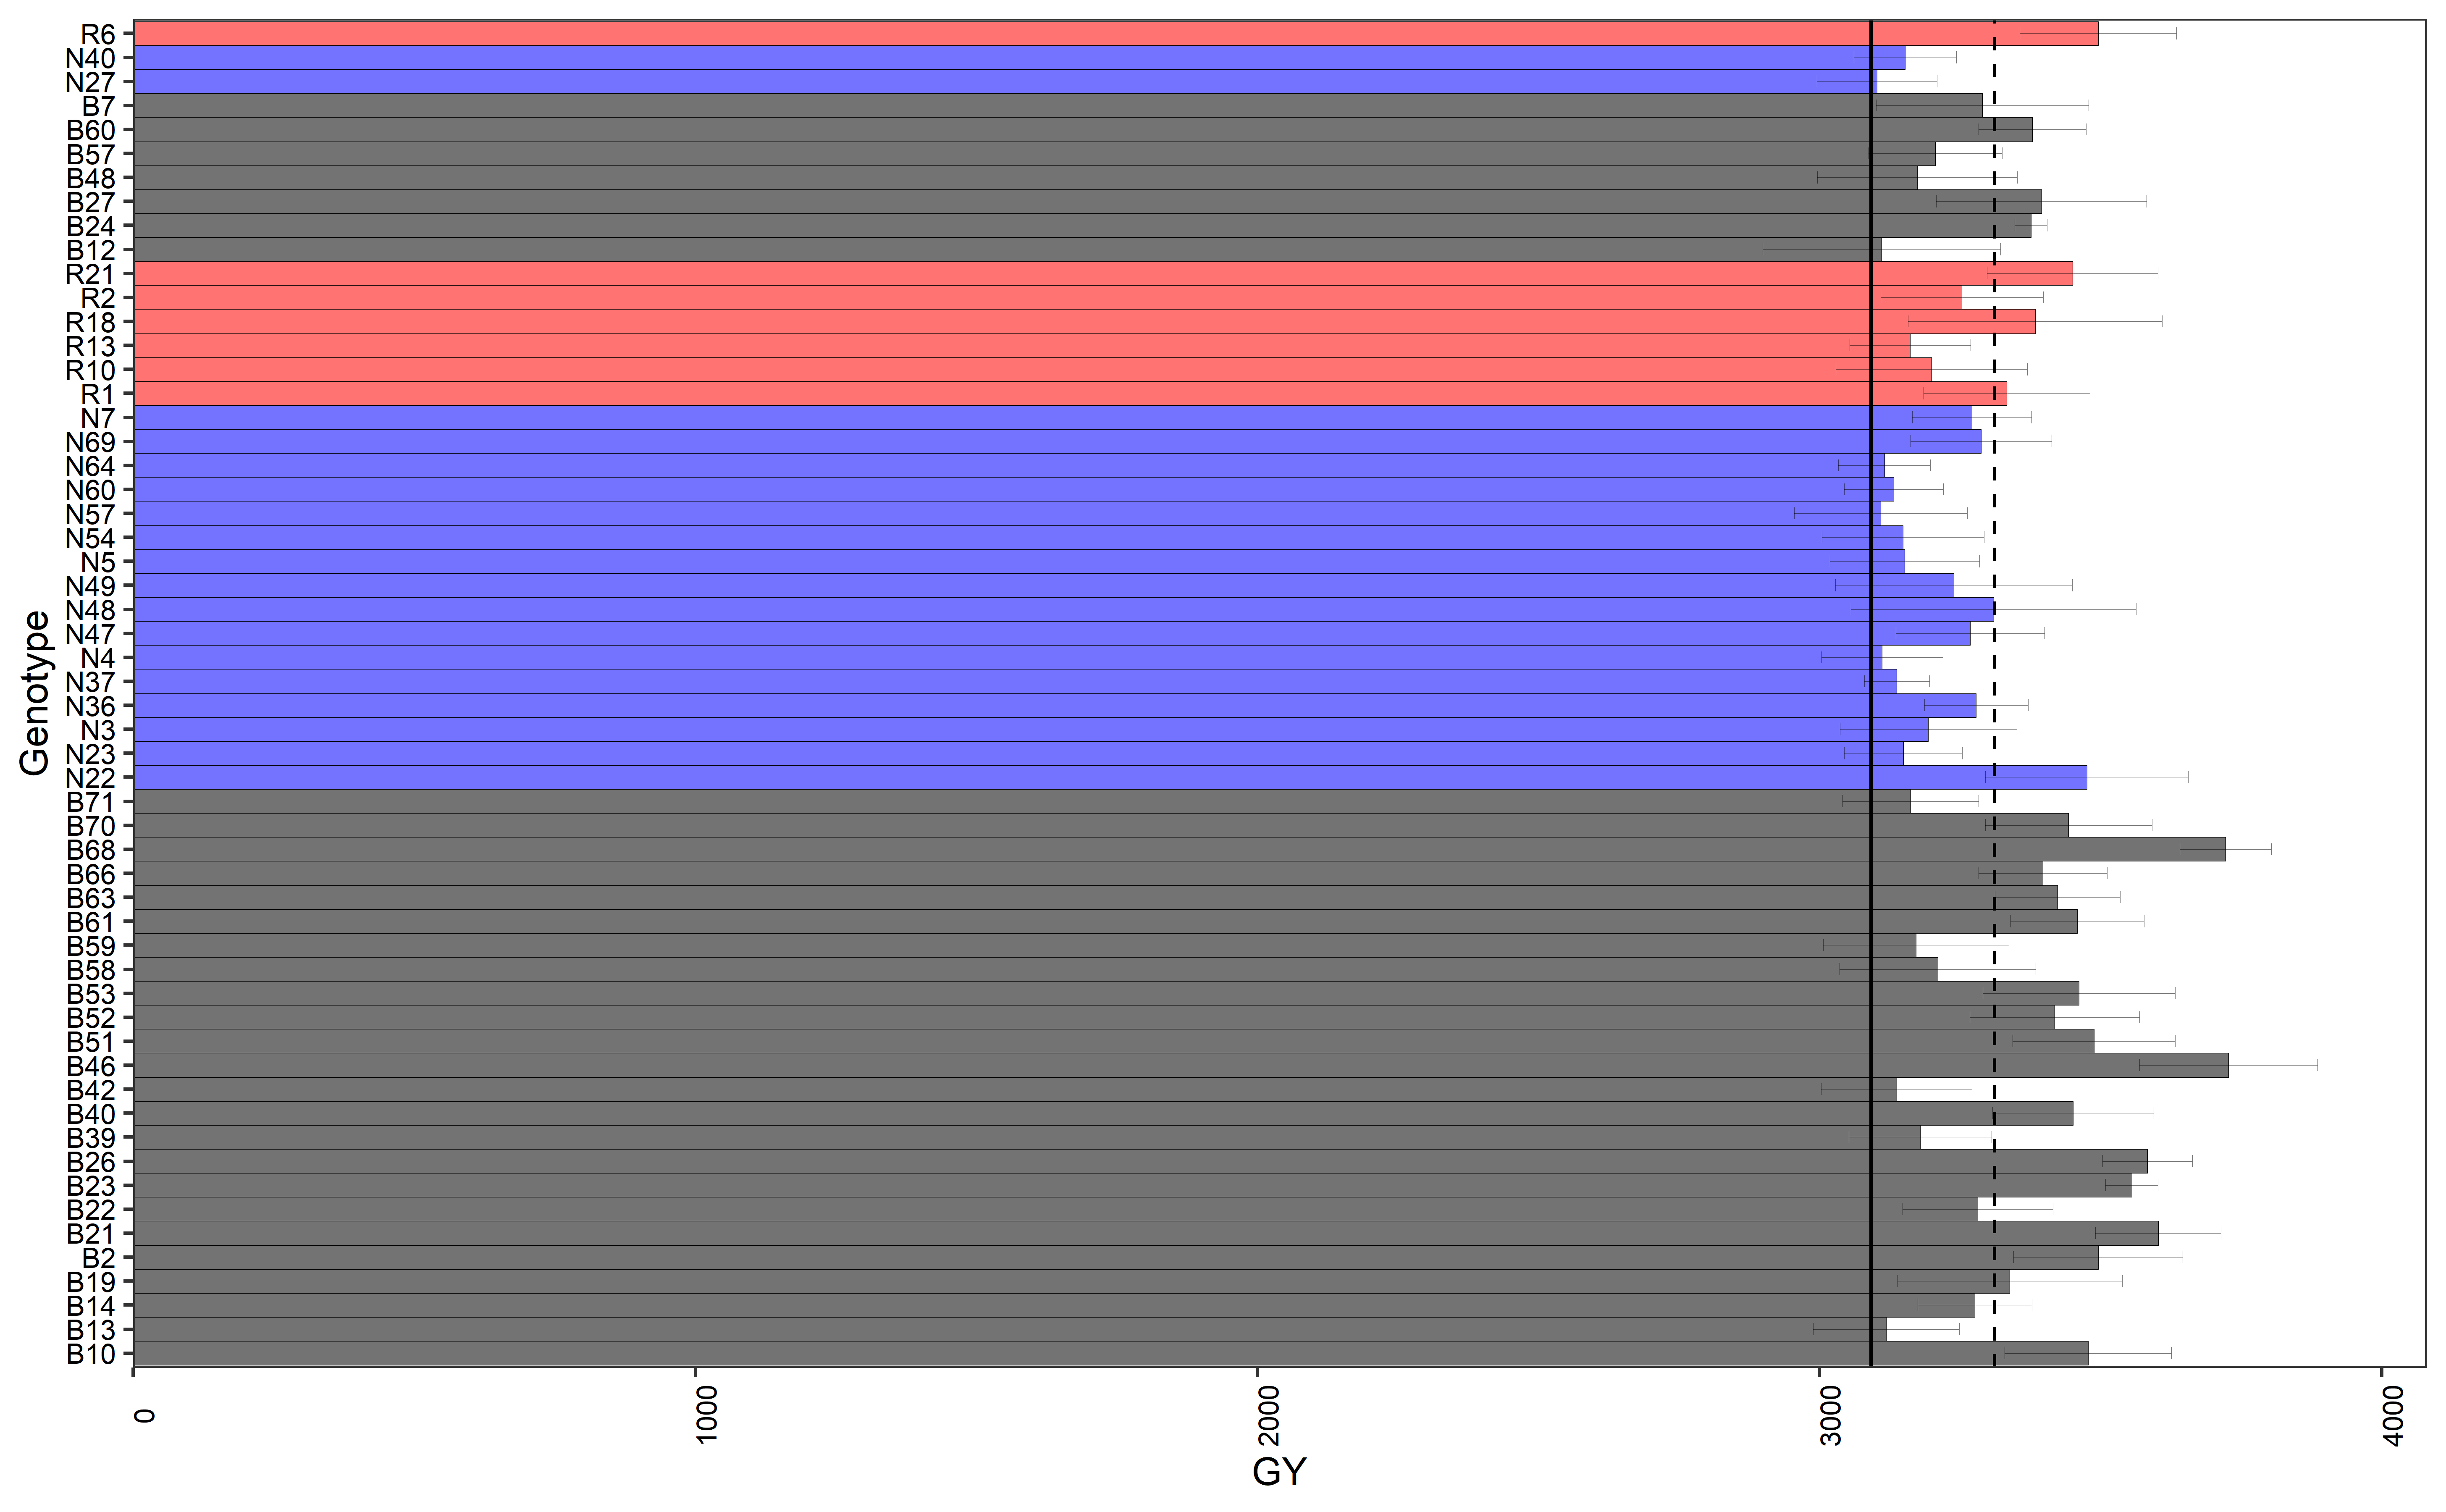
\includegraphics{figures/mod metan stab2-1} 

}

\caption{Mean performance for grain yield (GY) of all dry beans genotypes present in this study colored by market classes. The vertical dashed and solid lines shows, respectivelly, the mean of the selected genotype and the overall mean for both mean performance and WAASB index}\label{fig:mod metan stab2}
\end{figure}

\begin{Shaded}
\begin{Highlighting}[]
\NormalTok{p3}\OtherTok{\textless{}{-}} \FunctionTok{plot\_selected}\NormalTok{(waasb\_sel, GEN, WAASB\_sel, }\AttributeTok{mean\_sel =}\NormalTok{ waasb\_sel\_mean}\SpecialCharTok{$}\NormalTok{mean\_GY) }\SpecialCharTok{+}
  \FunctionTok{labs}\NormalTok{(}\AttributeTok{y =} \StringTok{"WAASB index"}\NormalTok{)}

\FunctionTok{arrange\_ggplot}\NormalTok{(p1, p3,}
  \AttributeTok{guides =} \StringTok{"collect"}\NormalTok{,}
  \AttributeTok{tag\_levels =} \StringTok{"a"}\NormalTok{,}
  \AttributeTok{tag\_prefix =} \StringTok{"("}\NormalTok{,}
  \AttributeTok{tag\_suffix =} \StringTok{")"}\NormalTok{)}
\end{Highlighting}
\end{Shaded}

\begin{figure}

{\centering 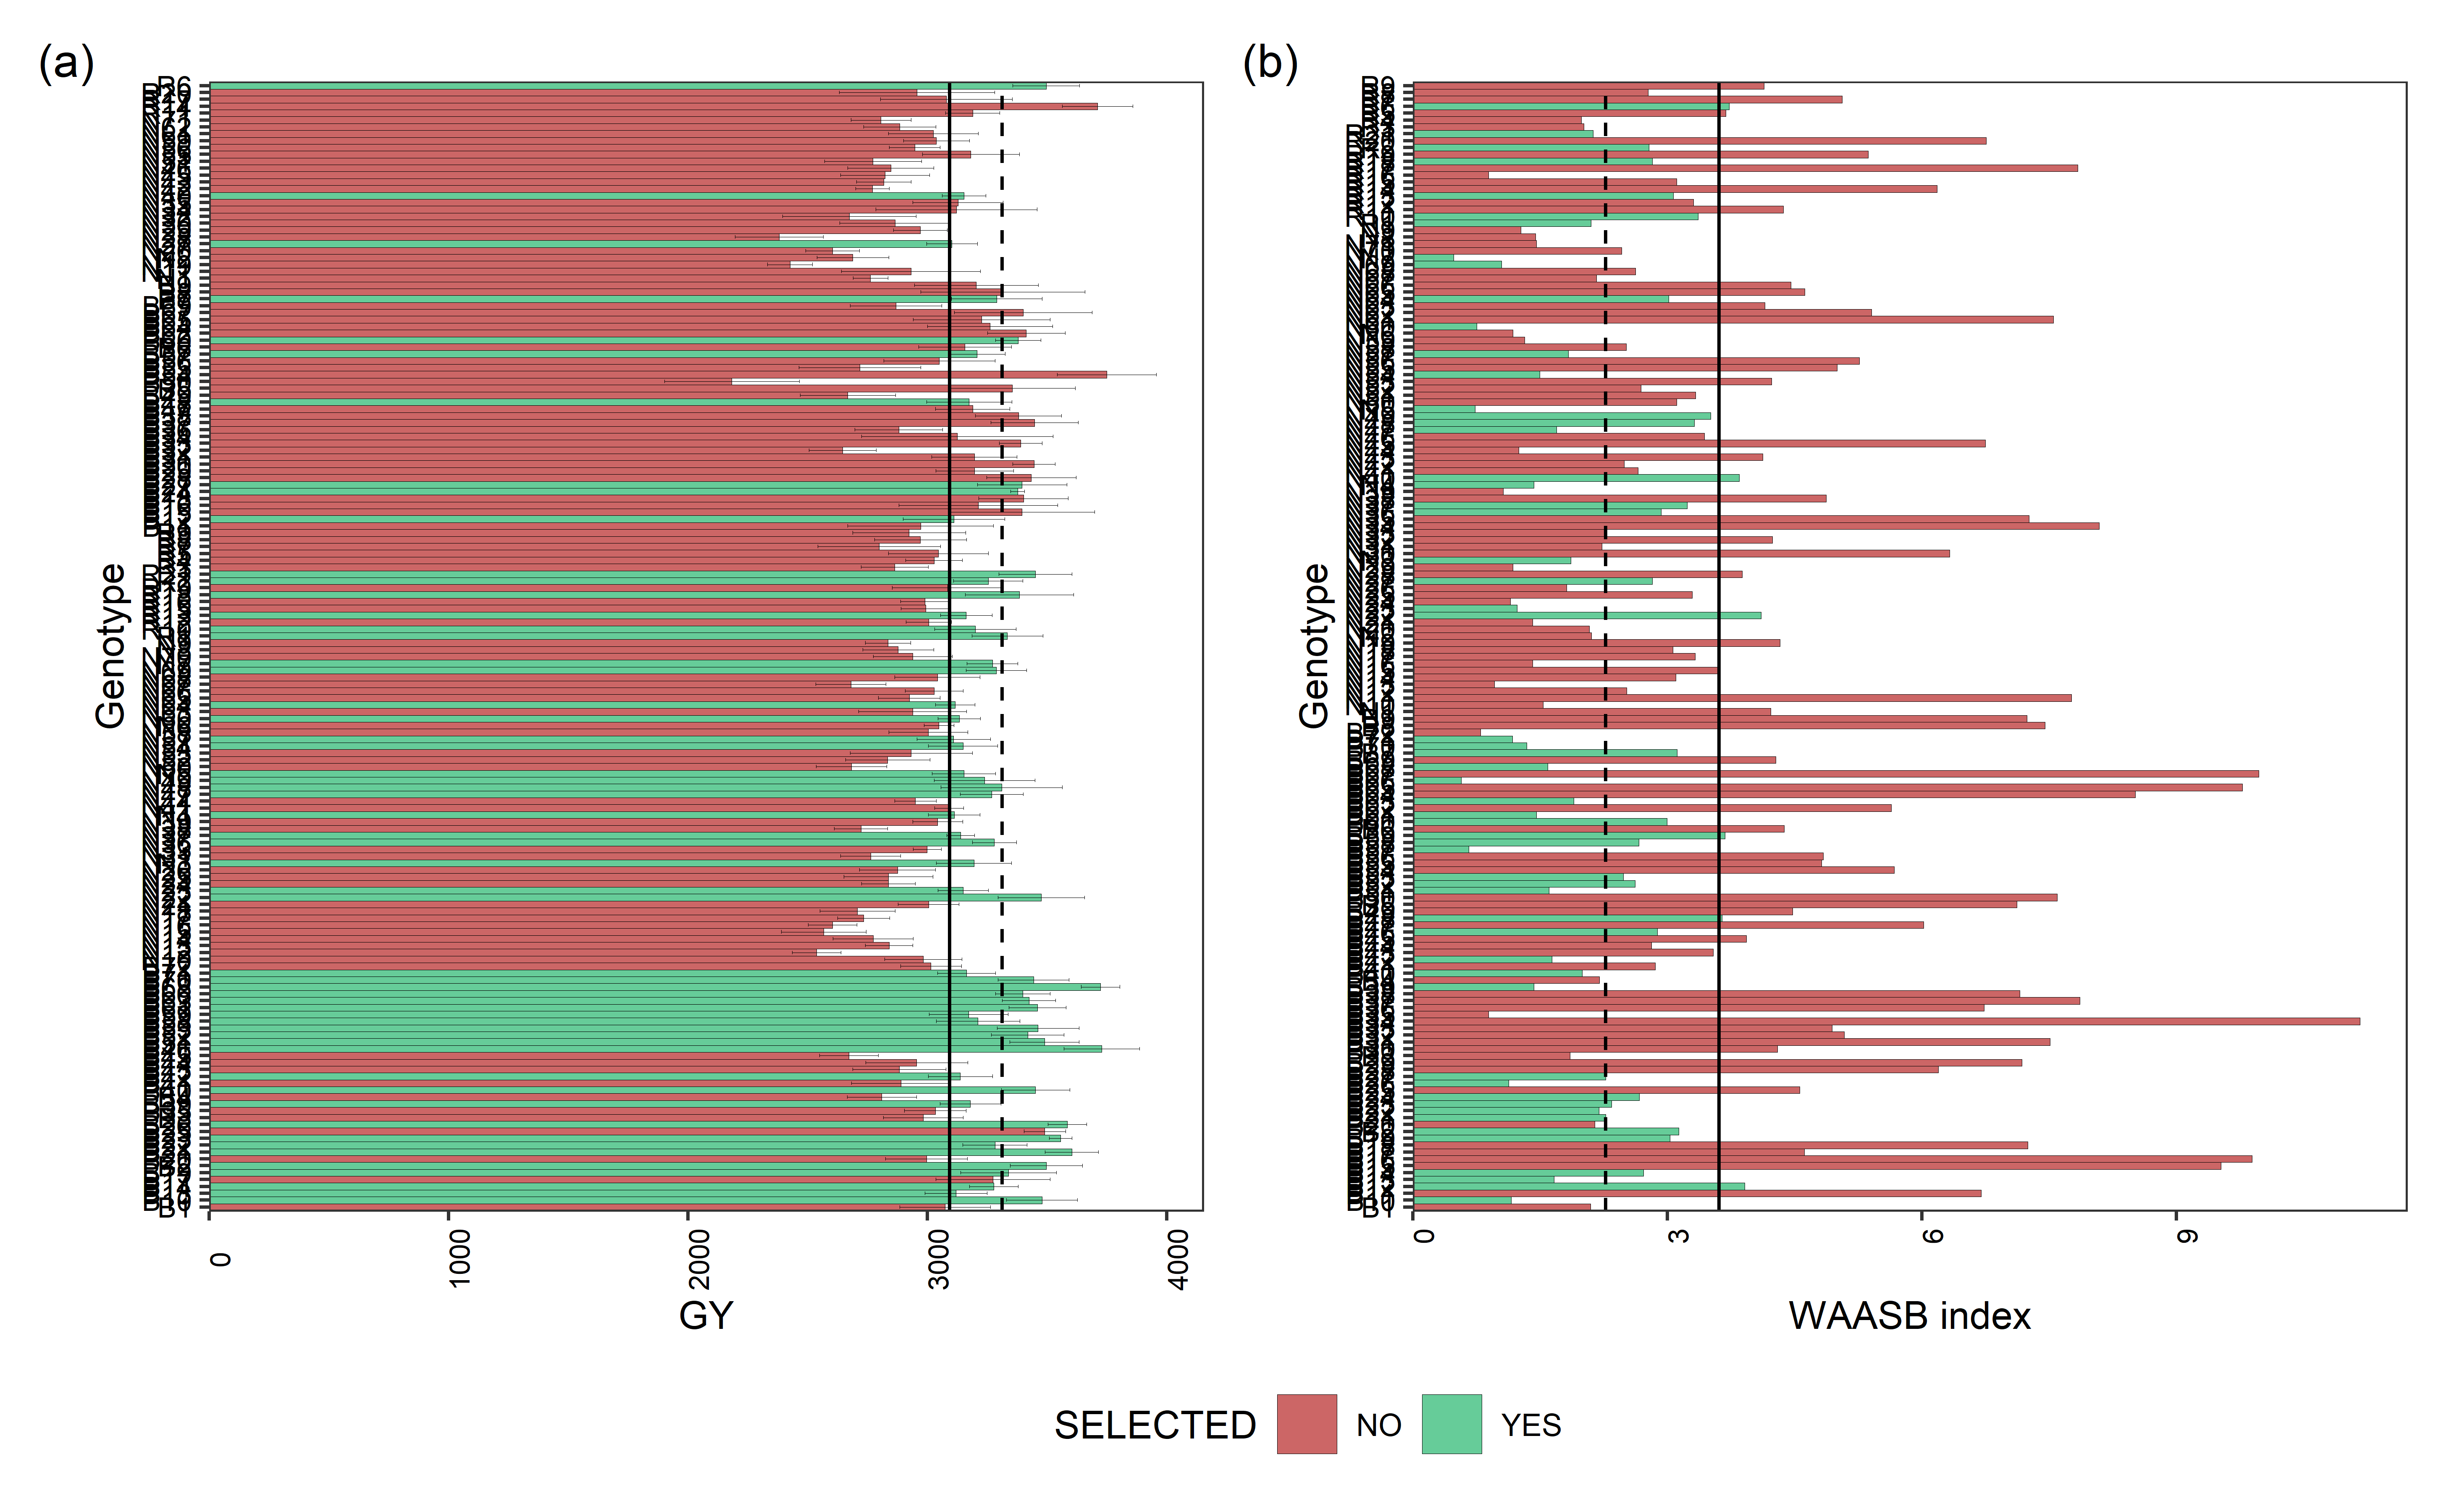
\includegraphics{figures/mod metan stab3-1} 

}

\caption{Mean performance (a) and stability (b) for grain yield (GY) for all dry beans genotypes present in this study. The vertical dashed and solid lines shows, respectivelly, the mean of the selected genotype and the overall mean for both mean performance and WAASB index}\label{fig:mod metan stab3}
\end{figure}

Percentage (SD\_gain in \%) gain from the selected genotypes compared to
the general mean.

\begin{Shaded}
\begin{Highlighting}[]
\NormalTok{blups\_sel2 }\OtherTok{\textless{}{-}}
  \FunctionTok{gmd}\NormalTok{(waasb\_model\_allMKT, }\StringTok{"blupg"}\NormalTok{) }\SpecialCharTok{\%\textgreater{}\%}
  \FunctionTok{add\_cols}\NormalTok{(}\AttributeTok{SELECTED =} \FunctionTok{ifelse}\NormalTok{(GEN }\SpecialCharTok{\%in\%}\NormalTok{ selected}\SpecialCharTok{$}\NormalTok{Code, }\StringTok{"yes"}\NormalTok{, }\StringTok{"no"}\NormalTok{)) }\SpecialCharTok{\%\textgreater{}\%} 
\NormalTok{    dplyr}\SpecialCharTok{::}\FunctionTok{rename}\NormalTok{(}\AttributeTok{BLUPs\_sel =}\NormalTok{ yield) }\SpecialCharTok{\%\textgreater{}\%} 
  \FunctionTok{droplevels}\NormalTok{()}
\end{Highlighting}
\end{Shaded}

\begin{verbatim}
#> Class of the model: waasb
\end{verbatim}

\begin{verbatim}
#> Variable extracted: blupg
\end{verbatim}

\begin{Shaded}
\begin{Highlighting}[]
\NormalTok{blups\_sel\_mean2}\OtherTok{\textless{}{-}}
  \FunctionTok{gmd}\NormalTok{(waasb\_model\_allMKT, }\StringTok{"blupg"}\NormalTok{) }\SpecialCharTok{\%\textgreater{}\%}
  \FunctionTok{add\_cols}\NormalTok{(}\AttributeTok{SELECTED =} \FunctionTok{ifelse}\NormalTok{(GEN }\SpecialCharTok{\%in\%}\NormalTok{ selected}\SpecialCharTok{$}\NormalTok{Code, }\StringTok{"yes"}\NormalTok{, }\StringTok{"no"}\NormalTok{)) }\SpecialCharTok{\%\textgreater{}\%} 
  \FunctionTok{filter}\NormalTok{(SELECTED }\SpecialCharTok{==} \StringTok{"yes"}\NormalTok{) }\SpecialCharTok{\%\textgreater{}\%} 
\NormalTok{  dplyr}\SpecialCharTok{::}\FunctionTok{summarise}\NormalTok{(}\AttributeTok{mean\_GY =} \FunctionTok{mean}\NormalTok{(yield,}\AttributeTok{na.rm =} \ConstantTok{TRUE}\NormalTok{), }\AttributeTok{n =} \FunctionTok{n}\NormalTok{()) }
\end{Highlighting}
\end{Shaded}

\begin{verbatim}
#> Class of the model: waasb
#> Variable extracted: blupg
\end{verbatim}

\begin{Shaded}
\begin{Highlighting}[]
\NormalTok{SD\_blups}\OtherTok{\textless{}{-}} \FunctionTok{as\_tibble}\NormalTok{((blups\_sel\_mean2}\SpecialCharTok{$}\NormalTok{mean\_GY}\SpecialCharTok{/}\FunctionTok{mean}\NormalTok{(blups\_sel2}\SpecialCharTok{$}\NormalTok{BLUPs\_sel, }\AttributeTok{na.rm =}\NormalTok{ T)) }\SpecialCharTok{{-}}\DecValTok{1}\NormalTok{)}\SpecialCharTok{*}\DecValTok{100}
\NormalTok{SD\_WAASP}\OtherTok{\textless{}{-}} \FunctionTok{as\_tibble}\NormalTok{((waasb\_sel\_mean}\SpecialCharTok{$}\NormalTok{mean\_GY }\SpecialCharTok{/}\FunctionTok{mean}\NormalTok{(waasb\_sel}\SpecialCharTok{$}\NormalTok{WAASB\_sel, }\AttributeTok{na.rm =}\NormalTok{ T)) }\SpecialCharTok{{-}}\DecValTok{1}\NormalTok{)}\SpecialCharTok{*}\DecValTok{100}

\NormalTok{SD\_comb}\OtherTok{\textless{}{-}} \FunctionTok{full\_join}\NormalTok{(SD\_blups, SD\_WAASP, }\AttributeTok{by =} \StringTok{"value"}\NormalTok{) }\SpecialCharTok{\%\textgreater{}\%} 
\NormalTok{  dplyr}\SpecialCharTok{::}\FunctionTok{rename}\NormalTok{(}\AttributeTok{SD\_gain =}\NormalTok{ value) }\SpecialCharTok{\%\textgreater{}\%} 
\NormalTok{  tibble}\SpecialCharTok{::}\FunctionTok{add\_column}\NormalTok{(}\AttributeTok{Comp\_name =} \FunctionTok{c}\NormalTok{(}\StringTok{\textquotesingle{}BLUPs\textquotesingle{}}\NormalTok{, }\StringTok{\textquotesingle{}WAASB\textquotesingle{}}\NormalTok{)) }\SpecialCharTok{\%\textgreater{}\%} 
  \FunctionTok{relocate}\NormalTok{(Comp\_name)}

\NormalTok{SD\_comb}\SpecialCharTok{$}\NormalTok{n\_selected}\OtherTok{\textless{}{-}}\NormalTok{ blups\_sel\_mean2}\SpecialCharTok{$}\NormalTok{n}
\NormalTok{SD\_comb}
\end{Highlighting}
\end{Shaded}

\global\setlength{\Oldarrayrulewidth}{\arrayrulewidth}

\global\setlength{\Oldtabcolsep}{\tabcolsep}

\setlength{\tabcolsep}{0pt}

\renewcommand*{\arraystretch}{1.5}



\providecommand{\ascline}[3]{\noalign{\global\arrayrulewidth #1}\arrayrulecolor[HTML]{#2}\cline{#3}}

\begin{longtable}[c]{|p{0.96in}|p{0.75in}|p{0.86in}}



\ascline{1.5pt}{666666}{1-3}

\multicolumn{1}{>{\raggedright}m{\dimexpr 0.96in+0\tabcolsep}}{\textcolor[HTML]{000000}{\fontsize{9}{9}\selectfont{\global\setmainfont{Arial}{\textbf{Comp\_name}}}}} & \multicolumn{1}{>{\raggedleft}m{\dimexpr 0.75in+0\tabcolsep}}{\textcolor[HTML]{000000}{\fontsize{9}{9}\selectfont{\global\setmainfont{Arial}{\textbf{SD\_gain}}}}} & \multicolumn{1}{>{\raggedleft}m{\dimexpr 0.86in+0\tabcolsep}}{\textcolor[HTML]{000000}{\fontsize{9}{9}\selectfont{\global\setmainfont{Arial}{\textbf{n\_selected}}}}} \\

\ascline{0.75pt}{666666}{1-3}



\multicolumn{1}{>{\raggedright}m{\dimexpr 0.96in+0\tabcolsep}}{\textcolor[HTML]{999999}{\fontsize{9}{9}\selectfont{\global\setmainfont{Arial}{\textbf{character}}}}} & \multicolumn{1}{>{\raggedleft}m{\dimexpr 0.75in+0\tabcolsep}}{\textcolor[HTML]{999999}{\fontsize{9}{9}\selectfont{\global\setmainfont{Arial}{\textbf{numeric}}}}} & \multicolumn{1}{>{\raggedleft}m{\dimexpr 0.86in+0\tabcolsep}}{\textcolor[HTML]{999999}{\fontsize{9}{9}\selectfont{\global\setmainfont{Arial}{\textbf{integer}}}}} \\

\ascline{1.5pt}{666666}{1-3}\endfirsthead

\ascline{1.5pt}{666666}{1-3}

\multicolumn{1}{>{\raggedright}m{\dimexpr 0.96in+0\tabcolsep}}{\textcolor[HTML]{000000}{\fontsize{9}{9}\selectfont{\global\setmainfont{Arial}{\textbf{Comp\_name}}}}} & \multicolumn{1}{>{\raggedleft}m{\dimexpr 0.75in+0\tabcolsep}}{\textcolor[HTML]{000000}{\fontsize{9}{9}\selectfont{\global\setmainfont{Arial}{\textbf{SD\_gain}}}}} & \multicolumn{1}{>{\raggedleft}m{\dimexpr 0.86in+0\tabcolsep}}{\textcolor[HTML]{000000}{\fontsize{9}{9}\selectfont{\global\setmainfont{Arial}{\textbf{n\_selected}}}}} \\

\ascline{0.75pt}{666666}{1-3}



\multicolumn{1}{>{\raggedright}m{\dimexpr 0.96in+0\tabcolsep}}{\textcolor[HTML]{999999}{\fontsize{9}{9}\selectfont{\global\setmainfont{Arial}{\textbf{character}}}}} & \multicolumn{1}{>{\raggedleft}m{\dimexpr 0.75in+0\tabcolsep}}{\textcolor[HTML]{999999}{\fontsize{9}{9}\selectfont{\global\setmainfont{Arial}{\textbf{numeric}}}}} & \multicolumn{1}{>{\raggedleft}m{\dimexpr 0.86in+0\tabcolsep}}{\textcolor[HTML]{999999}{\fontsize{9}{9}\selectfont{\global\setmainfont{Arial}{\textbf{integer}}}}} \\

\ascline{1.5pt}{666666}{1-3}\endhead



\multicolumn{3}{>{\raggedright}m{\dimexpr 2.57in+4\tabcolsep}}{\textcolor[HTML]{000000}{\fontsize{9}{9}\selectfont{\global\setmainfont{Arial}{n:\ 2}}}} \\

\ascline{0.75pt}{666666}{1-3}\endfoot



\multicolumn{1}{>{\raggedright}m{\dimexpr 0.96in+0\tabcolsep}}{\textcolor[HTML]{000000}{\fontsize{9}{9}\selectfont{\global\setmainfont{Arial}{BLUPs}}}} & \multicolumn{1}{>{\raggedleft}m{\dimexpr 0.75in+0\tabcolsep}}{\textcolor[HTML]{000000}{\fontsize{9}{9}\selectfont{\global\setmainfont{Arial}{4.9}}}} & \multicolumn{1}{>{\raggedleft}m{\dimexpr 0.86in+0\tabcolsep}}{\textcolor[HTML]{000000}{\fontsize{9}{9}\selectfont{\global\setmainfont{Arial}{56}}}} \\

\ascline{0.75pt}{666666}{1-3}



\multicolumn{1}{>{\raggedright}m{\dimexpr 0.96in+0\tabcolsep}}{\textcolor[HTML]{000000}{\fontsize{9}{9}\selectfont{\global\setmainfont{Arial}{WAASB}}}} & \multicolumn{1}{>{\raggedleft}m{\dimexpr 0.75in+0\tabcolsep}}{\textcolor[HTML]{000000}{\fontsize{9}{9}\selectfont{\global\setmainfont{Arial}{-37.1}}}} & \multicolumn{1}{>{\raggedleft}m{\dimexpr 0.86in+0\tabcolsep}}{\textcolor[HTML]{000000}{\fontsize{9}{9}\selectfont{\global\setmainfont{Arial}{56}}}} \\

\ascline{1.5pt}{666666}{1-3}



\end{longtable}



\arrayrulecolor[HTML]{000000}

\global\setlength{\arrayrulewidth}{\Oldarrayrulewidth}

\global\setlength{\tabcolsep}{\Oldtabcolsep}

\renewcommand*{\arraystretch}{1}

\begin{Shaded}
\begin{Highlighting}[]
\NormalTok{blups\_sel2}\SpecialCharTok{$}\NormalTok{mean\_blup }\OtherTok{\textless{}{-}} \FunctionTok{mean}\NormalTok{(blups\_sel2}\SpecialCharTok{$}\NormalTok{BLUPs\_sel, }\AttributeTok{na.rm =}\NormalTok{ T)}
\NormalTok{waasb\_sel}\SpecialCharTok{$}\NormalTok{mean\_waasb }\OtherTok{\textless{}{-}} \FunctionTok{mean}\NormalTok{(waasb\_sel}\SpecialCharTok{$}\NormalTok{WAASB\_sel, }\AttributeTok{na.rm =}\NormalTok{ T)}

\CommentTok{\#str(waasb\_sel)}
\NormalTok{data\_comb}\OtherTok{\textless{}{-}} \FunctionTok{merge}\NormalTok{(blups\_sel2, waasb\_sel, }\AttributeTok{by =} \FunctionTok{c}\NormalTok{(}\StringTok{"GEN"}\NormalTok{, }\StringTok{"SELECTED"}\NormalTok{))}
\CommentTok{\#names(data\_comb)}
\DocumentationTok{\#\# SD for each genotype}
\NormalTok{data\_sel\_perc }\OtherTok{\textless{}{-}}\NormalTok{ data\_comb }\SpecialCharTok{\%\textgreater{}\%}
\NormalTok{ rowwise }\SpecialCharTok{\%\textgreater{}\%}
  \FunctionTok{mutate}\NormalTok{(}\AttributeTok{Perc\_blup\_gain =}\NormalTok{ ((BLUPs\_sel}\SpecialCharTok{/}\NormalTok{mean\_blup)}\SpecialCharTok{*}\DecValTok{100}\NormalTok{)}\SpecialCharTok{{-}}\DecValTok{100}\NormalTok{) }\SpecialCharTok{\%\textgreater{}\%} 
  \FunctionTok{mutate}\NormalTok{(}\AttributeTok{Perc\_WAASB\_gain =}\NormalTok{ ((WAASB\_sel}\SpecialCharTok{/}\NormalTok{mean\_waasb)}\SpecialCharTok{*}\DecValTok{100}\NormalTok{)}\SpecialCharTok{{-}}\DecValTok{100}\NormalTok{) }\SpecialCharTok{\%\textgreater{}\%} 
  \FunctionTok{as\_tibble}\NormalTok{()}

\CommentTok{\# data\_sel\_perc\_mean \textless{}{-} data\_sel\_perc \%\textgreater{}\% }
\CommentTok{\#   dplyr::filter(SELECTED  == "yes")}
\CommentTok{\# }
\CommentTok{\# mean(data\_sel\_perc\_mean$Perc\_blup\_gain)}

\ControlFlowTok{if}\NormalTok{ (knitr}\SpecialCharTok{::}\FunctionTok{is\_html\_output}\NormalTok{()) \{}
  
\FunctionTok{print\_table}\NormalTok{(data\_sel\_perc)}
  
\NormalTok{\}}\ControlFlowTok{else}\NormalTok{\{}
  
\NormalTok{data\_sel\_perc[,}\DecValTok{1}\SpecialCharTok{:}\DecValTok{7}\NormalTok{]}
\NormalTok{\}}
\end{Highlighting}
\end{Shaded}

\global\setlength{\Oldarrayrulewidth}{\arrayrulewidth}

\global\setlength{\Oldtabcolsep}{\tabcolsep}

\setlength{\tabcolsep}{0pt}

\renewcommand*{\arraystretch}{1.5}



\providecommand{\ascline}[3]{\noalign{\global\arrayrulewidth #1}\arrayrulecolor[HTML]{#2}\cline{#3}}

\begin{longtable}[c]{|p{0.77in}|p{0.88in}|p{0.86in}|p{0.87in}|p{0.93in}|p{0.99in}|p{1.14in}}



\ascline{1.5pt}{666666}{1-7}

\multicolumn{1}{>{\raggedright}m{\dimexpr 0.77in+0\tabcolsep}}{\textcolor[HTML]{000000}{\fontsize{9}{9}\selectfont{\global\setmainfont{Arial}{\textbf{GEN}}}}} & \multicolumn{1}{>{\raggedright}m{\dimexpr 0.88in+0\tabcolsep}}{\textcolor[HTML]{000000}{\fontsize{9}{9}\selectfont{\global\setmainfont{Arial}{\textbf{SELECTED}}}}} & \multicolumn{1}{>{\raggedleft}m{\dimexpr 0.86in+0\tabcolsep}}{\textcolor[HTML]{000000}{\fontsize{9}{9}\selectfont{\global\setmainfont{Arial}{\textbf{BLUPs\_sel}}}}} & \multicolumn{1}{>{\raggedleft}m{\dimexpr 0.87in+0\tabcolsep}}{\textcolor[HTML]{000000}{\fontsize{9}{9}\selectfont{\global\setmainfont{Arial}{\textbf{mean\_blup}}}}} & \multicolumn{1}{>{\raggedleft}m{\dimexpr 0.93in+0\tabcolsep}}{\textcolor[HTML]{000000}{\fontsize{9}{9}\selectfont{\global\setmainfont{Arial}{\textbf{WAASB\_sel}}}}} & \multicolumn{1}{>{\raggedleft}m{\dimexpr 0.99in+0\tabcolsep}}{\textcolor[HTML]{000000}{\fontsize{9}{9}\selectfont{\global\setmainfont{Arial}{\textbf{mean\_waasb}}}}} & \multicolumn{1}{>{\raggedleft}m{\dimexpr 1.14in+0\tabcolsep}}{\textcolor[HTML]{000000}{\fontsize{9}{9}\selectfont{\global\setmainfont{Arial}{\textbf{Perc\_blup\_gain}}}}} \\

\ascline{0.75pt}{666666}{1-7}



\multicolumn{1}{>{\raggedright}m{\dimexpr 0.77in+0\tabcolsep}}{\textcolor[HTML]{999999}{\fontsize{9}{9}\selectfont{\global\setmainfont{Arial}{\textbf{character}}}}} & \multicolumn{1}{>{\raggedright}m{\dimexpr 0.88in+0\tabcolsep}}{\textcolor[HTML]{999999}{\fontsize{9}{9}\selectfont{\global\setmainfont{Arial}{\textbf{character}}}}} & \multicolumn{1}{>{\raggedleft}m{\dimexpr 0.86in+0\tabcolsep}}{\textcolor[HTML]{999999}{\fontsize{9}{9}\selectfont{\global\setmainfont{Arial}{\textbf{numeric}}}}} & \multicolumn{1}{>{\raggedleft}m{\dimexpr 0.87in+0\tabcolsep}}{\textcolor[HTML]{999999}{\fontsize{9}{9}\selectfont{\global\setmainfont{Arial}{\textbf{numeric}}}}} & \multicolumn{1}{>{\raggedleft}m{\dimexpr 0.93in+0\tabcolsep}}{\textcolor[HTML]{999999}{\fontsize{9}{9}\selectfont{\global\setmainfont{Arial}{\textbf{numeric}}}}} & \multicolumn{1}{>{\raggedleft}m{\dimexpr 0.99in+0\tabcolsep}}{\textcolor[HTML]{999999}{\fontsize{9}{9}\selectfont{\global\setmainfont{Arial}{\textbf{numeric}}}}} & \multicolumn{1}{>{\raggedleft}m{\dimexpr 1.14in+0\tabcolsep}}{\textcolor[HTML]{999999}{\fontsize{9}{9}\selectfont{\global\setmainfont{Arial}{\textbf{numeric}}}}} \\

\ascline{1.5pt}{666666}{1-7}\endfirsthead

\ascline{1.5pt}{666666}{1-7}

\multicolumn{1}{>{\raggedright}m{\dimexpr 0.77in+0\tabcolsep}}{\textcolor[HTML]{000000}{\fontsize{9}{9}\selectfont{\global\setmainfont{Arial}{\textbf{GEN}}}}} & \multicolumn{1}{>{\raggedright}m{\dimexpr 0.88in+0\tabcolsep}}{\textcolor[HTML]{000000}{\fontsize{9}{9}\selectfont{\global\setmainfont{Arial}{\textbf{SELECTED}}}}} & \multicolumn{1}{>{\raggedleft}m{\dimexpr 0.86in+0\tabcolsep}}{\textcolor[HTML]{000000}{\fontsize{9}{9}\selectfont{\global\setmainfont{Arial}{\textbf{BLUPs\_sel}}}}} & \multicolumn{1}{>{\raggedleft}m{\dimexpr 0.87in+0\tabcolsep}}{\textcolor[HTML]{000000}{\fontsize{9}{9}\selectfont{\global\setmainfont{Arial}{\textbf{mean\_blup}}}}} & \multicolumn{1}{>{\raggedleft}m{\dimexpr 0.93in+0\tabcolsep}}{\textcolor[HTML]{000000}{\fontsize{9}{9}\selectfont{\global\setmainfont{Arial}{\textbf{WAASB\_sel}}}}} & \multicolumn{1}{>{\raggedleft}m{\dimexpr 0.99in+0\tabcolsep}}{\textcolor[HTML]{000000}{\fontsize{9}{9}\selectfont{\global\setmainfont{Arial}{\textbf{mean\_waasb}}}}} & \multicolumn{1}{>{\raggedleft}m{\dimexpr 1.14in+0\tabcolsep}}{\textcolor[HTML]{000000}{\fontsize{9}{9}\selectfont{\global\setmainfont{Arial}{\textbf{Perc\_blup\_gain}}}}} \\

\ascline{0.75pt}{666666}{1-7}



\multicolumn{1}{>{\raggedright}m{\dimexpr 0.77in+0\tabcolsep}}{\textcolor[HTML]{999999}{\fontsize{9}{9}\selectfont{\global\setmainfont{Arial}{\textbf{character}}}}} & \multicolumn{1}{>{\raggedright}m{\dimexpr 0.88in+0\tabcolsep}}{\textcolor[HTML]{999999}{\fontsize{9}{9}\selectfont{\global\setmainfont{Arial}{\textbf{character}}}}} & \multicolumn{1}{>{\raggedleft}m{\dimexpr 0.86in+0\tabcolsep}}{\textcolor[HTML]{999999}{\fontsize{9}{9}\selectfont{\global\setmainfont{Arial}{\textbf{numeric}}}}} & \multicolumn{1}{>{\raggedleft}m{\dimexpr 0.87in+0\tabcolsep}}{\textcolor[HTML]{999999}{\fontsize{9}{9}\selectfont{\global\setmainfont{Arial}{\textbf{numeric}}}}} & \multicolumn{1}{>{\raggedleft}m{\dimexpr 0.93in+0\tabcolsep}}{\textcolor[HTML]{999999}{\fontsize{9}{9}\selectfont{\global\setmainfont{Arial}{\textbf{numeric}}}}} & \multicolumn{1}{>{\raggedleft}m{\dimexpr 0.99in+0\tabcolsep}}{\textcolor[HTML]{999999}{\fontsize{9}{9}\selectfont{\global\setmainfont{Arial}{\textbf{numeric}}}}} & \multicolumn{1}{>{\raggedleft}m{\dimexpr 1.14in+0\tabcolsep}}{\textcolor[HTML]{999999}{\fontsize{9}{9}\selectfont{\global\setmainfont{Arial}{\textbf{numeric}}}}} \\

\ascline{1.5pt}{666666}{1-7}\endhead



\multicolumn{7}{>{\raggedright}m{\dimexpr 6.44in+12\tabcolsep}}{\textcolor[HTML]{000000}{\fontsize{9}{9}\selectfont{\global\setmainfont{Arial}{n:\ 164}}}} \\

\ascline{0.75pt}{666666}{1-7}\endfoot



\multicolumn{1}{>{\raggedright}m{\dimexpr 0.77in+0\tabcolsep}}{\textcolor[HTML]{000000}{\fontsize{9}{9}\selectfont{\global\setmainfont{Arial}{B1}}}} & \multicolumn{1}{>{\raggedright}m{\dimexpr 0.88in+0\tabcolsep}}{\textcolor[HTML]{000000}{\fontsize{9}{9}\selectfont{\global\setmainfont{Arial}{no}}}} & \multicolumn{1}{>{\raggedleft}m{\dimexpr 0.86in+0\tabcolsep}}{\textcolor[HTML]{000000}{\fontsize{9}{9}\selectfont{\global\setmainfont{Arial}{3,088.8}}}} & \multicolumn{1}{>{\raggedleft}m{\dimexpr 0.87in+0\tabcolsep}}{\textcolor[HTML]{000000}{\fontsize{9}{9}\selectfont{\global\setmainfont{Arial}{3,097.9}}}} & \multicolumn{1}{>{\raggedleft}m{\dimexpr 0.93in+0\tabcolsep}}{\textcolor[HTML]{000000}{\fontsize{9}{9}\selectfont{\global\setmainfont{Arial}{2.1}}}} & \multicolumn{1}{>{\raggedleft}m{\dimexpr 0.99in+0\tabcolsep}}{\textcolor[HTML]{000000}{\fontsize{9}{9}\selectfont{\global\setmainfont{Arial}{3.6}}}} & \multicolumn{1}{>{\raggedleft}m{\dimexpr 1.14in+0\tabcolsep}}{\textcolor[HTML]{000000}{\fontsize{9}{9}\selectfont{\global\setmainfont{Arial}{-0.3}}}} \\

\ascline{0.75pt}{666666}{1-7}



\multicolumn{1}{>{\raggedright}m{\dimexpr 0.77in+0\tabcolsep}}{\textcolor[HTML]{000000}{\fontsize{9}{9}\selectfont{\global\setmainfont{Arial}{B10}}}} & \multicolumn{1}{>{\raggedright}m{\dimexpr 0.88in+0\tabcolsep}}{\textcolor[HTML]{000000}{\fontsize{9}{9}\selectfont{\global\setmainfont{Arial}{yes}}}} & \multicolumn{1}{>{\raggedleft}m{\dimexpr 0.86in+0\tabcolsep}}{\textcolor[HTML]{000000}{\fontsize{9}{9}\selectfont{\global\setmainfont{Arial}{3,365.6}}}} & \multicolumn{1}{>{\raggedleft}m{\dimexpr 0.87in+0\tabcolsep}}{\textcolor[HTML]{000000}{\fontsize{9}{9}\selectfont{\global\setmainfont{Arial}{3,097.9}}}} & \multicolumn{1}{>{\raggedleft}m{\dimexpr 0.93in+0\tabcolsep}}{\textcolor[HTML]{000000}{\fontsize{9}{9}\selectfont{\global\setmainfont{Arial}{1.2}}}} & \multicolumn{1}{>{\raggedleft}m{\dimexpr 0.99in+0\tabcolsep}}{\textcolor[HTML]{000000}{\fontsize{9}{9}\selectfont{\global\setmainfont{Arial}{3.6}}}} & \multicolumn{1}{>{\raggedleft}m{\dimexpr 1.14in+0\tabcolsep}}{\textcolor[HTML]{000000}{\fontsize{9}{9}\selectfont{\global\setmainfont{Arial}{8.6}}}} \\

\ascline{0.75pt}{666666}{1-7}



\multicolumn{1}{>{\raggedright}m{\dimexpr 0.77in+0\tabcolsep}}{\textcolor[HTML]{000000}{\fontsize{9}{9}\selectfont{\global\setmainfont{Arial}{B11}}}} & \multicolumn{1}{>{\raggedright}m{\dimexpr 0.88in+0\tabcolsep}}{\textcolor[HTML]{000000}{\fontsize{9}{9}\selectfont{\global\setmainfont{Arial}{no}}}} & \multicolumn{1}{>{\raggedleft}m{\dimexpr 0.86in+0\tabcolsep}}{\textcolor[HTML]{000000}{\fontsize{9}{9}\selectfont{\global\setmainfont{Arial}{3,001.6}}}} & \multicolumn{1}{>{\raggedleft}m{\dimexpr 0.87in+0\tabcolsep}}{\textcolor[HTML]{000000}{\fontsize{9}{9}\selectfont{\global\setmainfont{Arial}{3,097.9}}}} & \multicolumn{1}{>{\raggedleft}m{\dimexpr 0.93in+0\tabcolsep}}{\textcolor[HTML]{000000}{\fontsize{9}{9}\selectfont{\global\setmainfont{Arial}{6.7}}}} & \multicolumn{1}{>{\raggedleft}m{\dimexpr 0.99in+0\tabcolsep}}{\textcolor[HTML]{000000}{\fontsize{9}{9}\selectfont{\global\setmainfont{Arial}{3.6}}}} & \multicolumn{1}{>{\raggedleft}m{\dimexpr 1.14in+0\tabcolsep}}{\textcolor[HTML]{000000}{\fontsize{9}{9}\selectfont{\global\setmainfont{Arial}{-3.1}}}} \\

\ascline{0.75pt}{666666}{1-7}



\multicolumn{1}{>{\raggedright}m{\dimexpr 0.77in+0\tabcolsep}}{\textcolor[HTML]{000000}{\fontsize{9}{9}\selectfont{\global\setmainfont{Arial}{B12}}}} & \multicolumn{1}{>{\raggedright}m{\dimexpr 0.88in+0\tabcolsep}}{\textcolor[HTML]{000000}{\fontsize{9}{9}\selectfont{\global\setmainfont{Arial}{yes}}}} & \multicolumn{1}{>{\raggedleft}m{\dimexpr 0.86in+0\tabcolsep}}{\textcolor[HTML]{000000}{\fontsize{9}{9}\selectfont{\global\setmainfont{Arial}{3,097.1}}}} & \multicolumn{1}{>{\raggedleft}m{\dimexpr 0.87in+0\tabcolsep}}{\textcolor[HTML]{000000}{\fontsize{9}{9}\selectfont{\global\setmainfont{Arial}{3,097.9}}}} & \multicolumn{1}{>{\raggedleft}m{\dimexpr 0.93in+0\tabcolsep}}{\textcolor[HTML]{000000}{\fontsize{9}{9}\selectfont{\global\setmainfont{Arial}{3.9}}}} & \multicolumn{1}{>{\raggedleft}m{\dimexpr 0.99in+0\tabcolsep}}{\textcolor[HTML]{000000}{\fontsize{9}{9}\selectfont{\global\setmainfont{Arial}{3.6}}}} & \multicolumn{1}{>{\raggedleft}m{\dimexpr 1.14in+0\tabcolsep}}{\textcolor[HTML]{000000}{\fontsize{9}{9}\selectfont{\global\setmainfont{Arial}{-0.0}}}} \\

\ascline{0.75pt}{666666}{1-7}



\multicolumn{1}{>{\raggedright}m{\dimexpr 0.77in+0\tabcolsep}}{\textcolor[HTML]{000000}{\fontsize{9}{9}\selectfont{\global\setmainfont{Arial}{B13}}}} & \multicolumn{1}{>{\raggedright}m{\dimexpr 0.88in+0\tabcolsep}}{\textcolor[HTML]{000000}{\fontsize{9}{9}\selectfont{\global\setmainfont{Arial}{yes}}}} & \multicolumn{1}{>{\raggedleft}m{\dimexpr 0.86in+0\tabcolsep}}{\textcolor[HTML]{000000}{\fontsize{9}{9}\selectfont{\global\setmainfont{Arial}{3,119.3}}}} & \multicolumn{1}{>{\raggedleft}m{\dimexpr 0.87in+0\tabcolsep}}{\textcolor[HTML]{000000}{\fontsize{9}{9}\selectfont{\global\setmainfont{Arial}{3,097.9}}}} & \multicolumn{1}{>{\raggedleft}m{\dimexpr 0.93in+0\tabcolsep}}{\textcolor[HTML]{000000}{\fontsize{9}{9}\selectfont{\global\setmainfont{Arial}{1.7}}}} & \multicolumn{1}{>{\raggedleft}m{\dimexpr 0.99in+0\tabcolsep}}{\textcolor[HTML]{000000}{\fontsize{9}{9}\selectfont{\global\setmainfont{Arial}{3.6}}}} & \multicolumn{1}{>{\raggedleft}m{\dimexpr 1.14in+0\tabcolsep}}{\textcolor[HTML]{000000}{\fontsize{9}{9}\selectfont{\global\setmainfont{Arial}{0.7}}}} \\

\ascline{0.75pt}{666666}{1-7}



\multicolumn{1}{>{\raggedright}m{\dimexpr 0.77in+0\tabcolsep}}{\textcolor[HTML]{000000}{\fontsize{9}{9}\selectfont{\global\setmainfont{Arial}{B14}}}} & \multicolumn{1}{>{\raggedright}m{\dimexpr 0.88in+0\tabcolsep}}{\textcolor[HTML]{000000}{\fontsize{9}{9}\selectfont{\global\setmainfont{Arial}{yes}}}} & \multicolumn{1}{>{\raggedleft}m{\dimexpr 0.86in+0\tabcolsep}}{\textcolor[HTML]{000000}{\fontsize{9}{9}\selectfont{\global\setmainfont{Arial}{3,227.6}}}} & \multicolumn{1}{>{\raggedleft}m{\dimexpr 0.87in+0\tabcolsep}}{\textcolor[HTML]{000000}{\fontsize{9}{9}\selectfont{\global\setmainfont{Arial}{3,097.9}}}} & \multicolumn{1}{>{\raggedleft}m{\dimexpr 0.93in+0\tabcolsep}}{\textcolor[HTML]{000000}{\fontsize{9}{9}\selectfont{\global\setmainfont{Arial}{2.7}}}} & \multicolumn{1}{>{\raggedleft}m{\dimexpr 0.99in+0\tabcolsep}}{\textcolor[HTML]{000000}{\fontsize{9}{9}\selectfont{\global\setmainfont{Arial}{3.6}}}} & \multicolumn{1}{>{\raggedleft}m{\dimexpr 1.14in+0\tabcolsep}}{\textcolor[HTML]{000000}{\fontsize{9}{9}\selectfont{\global\setmainfont{Arial}{4.2}}}} \\

\ascline{0.75pt}{666666}{1-7}



\multicolumn{1}{>{\raggedright}m{\dimexpr 0.77in+0\tabcolsep}}{\textcolor[HTML]{000000}{\fontsize{9}{9}\selectfont{\global\setmainfont{Arial}{B15}}}} & \multicolumn{1}{>{\raggedright}m{\dimexpr 0.88in+0\tabcolsep}}{\textcolor[HTML]{000000}{\fontsize{9}{9}\selectfont{\global\setmainfont{Arial}{no}}}} & \multicolumn{1}{>{\raggedleft}m{\dimexpr 0.86in+0\tabcolsep}}{\textcolor[HTML]{000000}{\fontsize{9}{9}\selectfont{\global\setmainfont{Arial}{3,291.3}}}} & \multicolumn{1}{>{\raggedleft}m{\dimexpr 0.87in+0\tabcolsep}}{\textcolor[HTML]{000000}{\fontsize{9}{9}\selectfont{\global\setmainfont{Arial}{3,097.9}}}} & \multicolumn{1}{>{\raggedleft}m{\dimexpr 0.93in+0\tabcolsep}}{\textcolor[HTML]{000000}{\fontsize{9}{9}\selectfont{\global\setmainfont{Arial}{9.5}}}} & \multicolumn{1}{>{\raggedleft}m{\dimexpr 0.99in+0\tabcolsep}}{\textcolor[HTML]{000000}{\fontsize{9}{9}\selectfont{\global\setmainfont{Arial}{3.6}}}} & \multicolumn{1}{>{\raggedleft}m{\dimexpr 1.14in+0\tabcolsep}}{\textcolor[HTML]{000000}{\fontsize{9}{9}\selectfont{\global\setmainfont{Arial}{6.2}}}} \\

\ascline{0.75pt}{666666}{1-7}



\multicolumn{1}{>{\raggedright}m{\dimexpr 0.77in+0\tabcolsep}}{\textcolor[HTML]{000000}{\fontsize{9}{9}\selectfont{\global\setmainfont{Arial}{B16}}}} & \multicolumn{1}{>{\raggedright}m{\dimexpr 0.88in+0\tabcolsep}}{\textcolor[HTML]{000000}{\fontsize{9}{9}\selectfont{\global\setmainfont{Arial}{no}}}} & \multicolumn{1}{>{\raggedleft}m{\dimexpr 0.86in+0\tabcolsep}}{\textcolor[HTML]{000000}{\fontsize{9}{9}\selectfont{\global\setmainfont{Arial}{3,166.7}}}} & \multicolumn{1}{>{\raggedleft}m{\dimexpr 0.87in+0\tabcolsep}}{\textcolor[HTML]{000000}{\fontsize{9}{9}\selectfont{\global\setmainfont{Arial}{3,097.9}}}} & \multicolumn{1}{>{\raggedleft}m{\dimexpr 0.93in+0\tabcolsep}}{\textcolor[HTML]{000000}{\fontsize{9}{9}\selectfont{\global\setmainfont{Arial}{9.9}}}} & \multicolumn{1}{>{\raggedleft}m{\dimexpr 0.99in+0\tabcolsep}}{\textcolor[HTML]{000000}{\fontsize{9}{9}\selectfont{\global\setmainfont{Arial}{3.6}}}} & \multicolumn{1}{>{\raggedleft}m{\dimexpr 1.14in+0\tabcolsep}}{\textcolor[HTML]{000000}{\fontsize{9}{9}\selectfont{\global\setmainfont{Arial}{2.2}}}} \\

\ascline{0.75pt}{666666}{1-7}



\multicolumn{1}{>{\raggedright}m{\dimexpr 0.77in+0\tabcolsep}}{\textcolor[HTML]{000000}{\fontsize{9}{9}\selectfont{\global\setmainfont{Arial}{B17}}}} & \multicolumn{1}{>{\raggedright}m{\dimexpr 0.88in+0\tabcolsep}}{\textcolor[HTML]{000000}{\fontsize{9}{9}\selectfont{\global\setmainfont{Arial}{no}}}} & \multicolumn{1}{>{\raggedleft}m{\dimexpr 0.86in+0\tabcolsep}}{\textcolor[HTML]{000000}{\fontsize{9}{9}\selectfont{\global\setmainfont{Arial}{3,225.7}}}} & \multicolumn{1}{>{\raggedleft}m{\dimexpr 0.87in+0\tabcolsep}}{\textcolor[HTML]{000000}{\fontsize{9}{9}\selectfont{\global\setmainfont{Arial}{3,097.9}}}} & \multicolumn{1}{>{\raggedleft}m{\dimexpr 0.93in+0\tabcolsep}}{\textcolor[HTML]{000000}{\fontsize{9}{9}\selectfont{\global\setmainfont{Arial}{4.6}}}} & \multicolumn{1}{>{\raggedleft}m{\dimexpr 0.99in+0\tabcolsep}}{\textcolor[HTML]{000000}{\fontsize{9}{9}\selectfont{\global\setmainfont{Arial}{3.6}}}} & \multicolumn{1}{>{\raggedleft}m{\dimexpr 1.14in+0\tabcolsep}}{\textcolor[HTML]{000000}{\fontsize{9}{9}\selectfont{\global\setmainfont{Arial}{4.1}}}} \\

\ascline{1.5pt}{666666}{1-7}



\end{longtable}



\arrayrulecolor[HTML]{000000}

\global\setlength{\arrayrulewidth}{\Oldarrayrulewidth}

\global\setlength{\tabcolsep}{\Oldtabcolsep}

\renewcommand*{\arraystretch}{1}

\begin{Shaded}
\begin{Highlighting}[]
\NormalTok{data\_sel\_perc}\OtherTok{\textless{}{-}}\NormalTok{ data\_sel\_perc }\SpecialCharTok{\%\textgreater{}\%} 
\NormalTok{  dplyr}\SpecialCharTok{::}\FunctionTok{relocate}\NormalTok{(GEN,SELECTED,BLUPs\_sel,mean\_blup,Perc\_blup\_gain,}
\NormalTok{                 WAASB\_sel,mean\_waasb ,Perc\_WAASB\_gain)}

\CommentTok{\#write.xlsx(data\_sel\_perc, "./data/sel\_SD\_bb\_2.xlsx")}

\NormalTok{data\_sel\_perc2 }\OtherTok{\textless{}{-}}\NormalTok{ data\_sel\_perc }\SpecialCharTok{\%\textgreater{}\%} 
\NormalTok{  dplyr}\SpecialCharTok{::}\FunctionTok{select}\NormalTok{(GEN,SELECTED, BLUPs\_sel, WAASB\_sel, Perc\_blup\_gain, Perc\_WAASB\_gain)}

\NormalTok{data\_sel\_perc2}
\end{Highlighting}
\end{Shaded}

\global\setlength{\Oldarrayrulewidth}{\arrayrulewidth}

\global\setlength{\Oldtabcolsep}{\tabcolsep}

\setlength{\tabcolsep}{0pt}

\renewcommand*{\arraystretch}{1.5}



\providecommand{\ascline}[3]{\noalign{\global\arrayrulewidth #1}\arrayrulecolor[HTML]{#2}\cline{#3}}

\begin{longtable}[c]{|p{0.77in}|p{0.88in}|p{0.86in}|p{0.93in}|p{1.14in}|p{1.35in}}



\ascline{1.5pt}{666666}{1-6}

\multicolumn{1}{>{\raggedright}m{\dimexpr 0.77in+0\tabcolsep}}{\textcolor[HTML]{000000}{\fontsize{9}{9}\selectfont{\global\setmainfont{Arial}{\textbf{GEN}}}}} & \multicolumn{1}{>{\raggedright}m{\dimexpr 0.88in+0\tabcolsep}}{\textcolor[HTML]{000000}{\fontsize{9}{9}\selectfont{\global\setmainfont{Arial}{\textbf{SELECTED}}}}} & \multicolumn{1}{>{\raggedleft}m{\dimexpr 0.86in+0\tabcolsep}}{\textcolor[HTML]{000000}{\fontsize{9}{9}\selectfont{\global\setmainfont{Arial}{\textbf{BLUPs\_sel}}}}} & \multicolumn{1}{>{\raggedleft}m{\dimexpr 0.93in+0\tabcolsep}}{\textcolor[HTML]{000000}{\fontsize{9}{9}\selectfont{\global\setmainfont{Arial}{\textbf{WAASB\_sel}}}}} & \multicolumn{1}{>{\raggedleft}m{\dimexpr 1.14in+0\tabcolsep}}{\textcolor[HTML]{000000}{\fontsize{9}{9}\selectfont{\global\setmainfont{Arial}{\textbf{Perc\_blup\_gain}}}}} & \multicolumn{1}{>{\raggedleft}m{\dimexpr 1.35in+0\tabcolsep}}{\textcolor[HTML]{000000}{\fontsize{9}{9}\selectfont{\global\setmainfont{Arial}{\textbf{Perc\_WAASB\_gain}}}}} \\

\ascline{0.75pt}{666666}{1-6}



\multicolumn{1}{>{\raggedright}m{\dimexpr 0.77in+0\tabcolsep}}{\textcolor[HTML]{999999}{\fontsize{9}{9}\selectfont{\global\setmainfont{Arial}{\textbf{character}}}}} & \multicolumn{1}{>{\raggedright}m{\dimexpr 0.88in+0\tabcolsep}}{\textcolor[HTML]{999999}{\fontsize{9}{9}\selectfont{\global\setmainfont{Arial}{\textbf{character}}}}} & \multicolumn{1}{>{\raggedleft}m{\dimexpr 0.86in+0\tabcolsep}}{\textcolor[HTML]{999999}{\fontsize{9}{9}\selectfont{\global\setmainfont{Arial}{\textbf{numeric}}}}} & \multicolumn{1}{>{\raggedleft}m{\dimexpr 0.93in+0\tabcolsep}}{\textcolor[HTML]{999999}{\fontsize{9}{9}\selectfont{\global\setmainfont{Arial}{\textbf{numeric}}}}} & \multicolumn{1}{>{\raggedleft}m{\dimexpr 1.14in+0\tabcolsep}}{\textcolor[HTML]{999999}{\fontsize{9}{9}\selectfont{\global\setmainfont{Arial}{\textbf{numeric}}}}} & \multicolumn{1}{>{\raggedleft}m{\dimexpr 1.35in+0\tabcolsep}}{\textcolor[HTML]{999999}{\fontsize{9}{9}\selectfont{\global\setmainfont{Arial}{\textbf{numeric}}}}} \\

\ascline{1.5pt}{666666}{1-6}\endfirsthead

\ascline{1.5pt}{666666}{1-6}

\multicolumn{1}{>{\raggedright}m{\dimexpr 0.77in+0\tabcolsep}}{\textcolor[HTML]{000000}{\fontsize{9}{9}\selectfont{\global\setmainfont{Arial}{\textbf{GEN}}}}} & \multicolumn{1}{>{\raggedright}m{\dimexpr 0.88in+0\tabcolsep}}{\textcolor[HTML]{000000}{\fontsize{9}{9}\selectfont{\global\setmainfont{Arial}{\textbf{SELECTED}}}}} & \multicolumn{1}{>{\raggedleft}m{\dimexpr 0.86in+0\tabcolsep}}{\textcolor[HTML]{000000}{\fontsize{9}{9}\selectfont{\global\setmainfont{Arial}{\textbf{BLUPs\_sel}}}}} & \multicolumn{1}{>{\raggedleft}m{\dimexpr 0.93in+0\tabcolsep}}{\textcolor[HTML]{000000}{\fontsize{9}{9}\selectfont{\global\setmainfont{Arial}{\textbf{WAASB\_sel}}}}} & \multicolumn{1}{>{\raggedleft}m{\dimexpr 1.14in+0\tabcolsep}}{\textcolor[HTML]{000000}{\fontsize{9}{9}\selectfont{\global\setmainfont{Arial}{\textbf{Perc\_blup\_gain}}}}} & \multicolumn{1}{>{\raggedleft}m{\dimexpr 1.35in+0\tabcolsep}}{\textcolor[HTML]{000000}{\fontsize{9}{9}\selectfont{\global\setmainfont{Arial}{\textbf{Perc\_WAASB\_gain}}}}} \\

\ascline{0.75pt}{666666}{1-6}



\multicolumn{1}{>{\raggedright}m{\dimexpr 0.77in+0\tabcolsep}}{\textcolor[HTML]{999999}{\fontsize{9}{9}\selectfont{\global\setmainfont{Arial}{\textbf{character}}}}} & \multicolumn{1}{>{\raggedright}m{\dimexpr 0.88in+0\tabcolsep}}{\textcolor[HTML]{999999}{\fontsize{9}{9}\selectfont{\global\setmainfont{Arial}{\textbf{character}}}}} & \multicolumn{1}{>{\raggedleft}m{\dimexpr 0.86in+0\tabcolsep}}{\textcolor[HTML]{999999}{\fontsize{9}{9}\selectfont{\global\setmainfont{Arial}{\textbf{numeric}}}}} & \multicolumn{1}{>{\raggedleft}m{\dimexpr 0.93in+0\tabcolsep}}{\textcolor[HTML]{999999}{\fontsize{9}{9}\selectfont{\global\setmainfont{Arial}{\textbf{numeric}}}}} & \multicolumn{1}{>{\raggedleft}m{\dimexpr 1.14in+0\tabcolsep}}{\textcolor[HTML]{999999}{\fontsize{9}{9}\selectfont{\global\setmainfont{Arial}{\textbf{numeric}}}}} & \multicolumn{1}{>{\raggedleft}m{\dimexpr 1.35in+0\tabcolsep}}{\textcolor[HTML]{999999}{\fontsize{9}{9}\selectfont{\global\setmainfont{Arial}{\textbf{numeric}}}}} \\

\ascline{1.5pt}{666666}{1-6}\endhead



\multicolumn{6}{>{\raggedright}m{\dimexpr 5.93in+10\tabcolsep}}{\textcolor[HTML]{000000}{\fontsize{9}{9}\selectfont{\global\setmainfont{Arial}{n:\ 164}}}} \\

\ascline{0.75pt}{666666}{1-6}\endfoot



\multicolumn{1}{>{\raggedright}m{\dimexpr 0.77in+0\tabcolsep}}{\textcolor[HTML]{000000}{\fontsize{9}{9}\selectfont{\global\setmainfont{Arial}{B1}}}} & \multicolumn{1}{>{\raggedright}m{\dimexpr 0.88in+0\tabcolsep}}{\textcolor[HTML]{000000}{\fontsize{9}{9}\selectfont{\global\setmainfont{Arial}{no}}}} & \multicolumn{1}{>{\raggedleft}m{\dimexpr 0.86in+0\tabcolsep}}{\textcolor[HTML]{000000}{\fontsize{9}{9}\selectfont{\global\setmainfont{Arial}{3,088.8}}}} & \multicolumn{1}{>{\raggedleft}m{\dimexpr 0.93in+0\tabcolsep}}{\textcolor[HTML]{000000}{\fontsize{9}{9}\selectfont{\global\setmainfont{Arial}{2.1}}}} & \multicolumn{1}{>{\raggedleft}m{\dimexpr 1.14in+0\tabcolsep}}{\textcolor[HTML]{000000}{\fontsize{9}{9}\selectfont{\global\setmainfont{Arial}{-0.3}}}} & \multicolumn{1}{>{\raggedleft}m{\dimexpr 1.35in+0\tabcolsep}}{\textcolor[HTML]{000000}{\fontsize{9}{9}\selectfont{\global\setmainfont{Arial}{-42.0}}}} \\

\ascline{0.75pt}{666666}{1-6}



\multicolumn{1}{>{\raggedright}m{\dimexpr 0.77in+0\tabcolsep}}{\textcolor[HTML]{000000}{\fontsize{9}{9}\selectfont{\global\setmainfont{Arial}{B10}}}} & \multicolumn{1}{>{\raggedright}m{\dimexpr 0.88in+0\tabcolsep}}{\textcolor[HTML]{000000}{\fontsize{9}{9}\selectfont{\global\setmainfont{Arial}{yes}}}} & \multicolumn{1}{>{\raggedleft}m{\dimexpr 0.86in+0\tabcolsep}}{\textcolor[HTML]{000000}{\fontsize{9}{9}\selectfont{\global\setmainfont{Arial}{3,365.6}}}} & \multicolumn{1}{>{\raggedleft}m{\dimexpr 0.93in+0\tabcolsep}}{\textcolor[HTML]{000000}{\fontsize{9}{9}\selectfont{\global\setmainfont{Arial}{1.2}}}} & \multicolumn{1}{>{\raggedleft}m{\dimexpr 1.14in+0\tabcolsep}}{\textcolor[HTML]{000000}{\fontsize{9}{9}\selectfont{\global\setmainfont{Arial}{8.6}}}} & \multicolumn{1}{>{\raggedleft}m{\dimexpr 1.35in+0\tabcolsep}}{\textcolor[HTML]{000000}{\fontsize{9}{9}\selectfont{\global\setmainfont{Arial}{-68.0}}}} \\

\ascline{0.75pt}{666666}{1-6}



\multicolumn{1}{>{\raggedright}m{\dimexpr 0.77in+0\tabcolsep}}{\textcolor[HTML]{000000}{\fontsize{9}{9}\selectfont{\global\setmainfont{Arial}{B11}}}} & \multicolumn{1}{>{\raggedright}m{\dimexpr 0.88in+0\tabcolsep}}{\textcolor[HTML]{000000}{\fontsize{9}{9}\selectfont{\global\setmainfont{Arial}{no}}}} & \multicolumn{1}{>{\raggedleft}m{\dimexpr 0.86in+0\tabcolsep}}{\textcolor[HTML]{000000}{\fontsize{9}{9}\selectfont{\global\setmainfont{Arial}{3,001.6}}}} & \multicolumn{1}{>{\raggedleft}m{\dimexpr 0.93in+0\tabcolsep}}{\textcolor[HTML]{000000}{\fontsize{9}{9}\selectfont{\global\setmainfont{Arial}{6.7}}}} & \multicolumn{1}{>{\raggedleft}m{\dimexpr 1.14in+0\tabcolsep}}{\textcolor[HTML]{000000}{\fontsize{9}{9}\selectfont{\global\setmainfont{Arial}{-3.1}}}} & \multicolumn{1}{>{\raggedleft}m{\dimexpr 1.35in+0\tabcolsep}}{\textcolor[HTML]{000000}{\fontsize{9}{9}\selectfont{\global\setmainfont{Arial}{85.5}}}} \\

\ascline{0.75pt}{666666}{1-6}



\multicolumn{1}{>{\raggedright}m{\dimexpr 0.77in+0\tabcolsep}}{\textcolor[HTML]{000000}{\fontsize{9}{9}\selectfont{\global\setmainfont{Arial}{B12}}}} & \multicolumn{1}{>{\raggedright}m{\dimexpr 0.88in+0\tabcolsep}}{\textcolor[HTML]{000000}{\fontsize{9}{9}\selectfont{\global\setmainfont{Arial}{yes}}}} & \multicolumn{1}{>{\raggedleft}m{\dimexpr 0.86in+0\tabcolsep}}{\textcolor[HTML]{000000}{\fontsize{9}{9}\selectfont{\global\setmainfont{Arial}{3,097.1}}}} & \multicolumn{1}{>{\raggedleft}m{\dimexpr 0.93in+0\tabcolsep}}{\textcolor[HTML]{000000}{\fontsize{9}{9}\selectfont{\global\setmainfont{Arial}{3.9}}}} & \multicolumn{1}{>{\raggedleft}m{\dimexpr 1.14in+0\tabcolsep}}{\textcolor[HTML]{000000}{\fontsize{9}{9}\selectfont{\global\setmainfont{Arial}{-0.0}}}} & \multicolumn{1}{>{\raggedleft}m{\dimexpr 1.35in+0\tabcolsep}}{\textcolor[HTML]{000000}{\fontsize{9}{9}\selectfont{\global\setmainfont{Arial}{8.2}}}} \\

\ascline{0.75pt}{666666}{1-6}



\multicolumn{1}{>{\raggedright}m{\dimexpr 0.77in+0\tabcolsep}}{\textcolor[HTML]{000000}{\fontsize{9}{9}\selectfont{\global\setmainfont{Arial}{B13}}}} & \multicolumn{1}{>{\raggedright}m{\dimexpr 0.88in+0\tabcolsep}}{\textcolor[HTML]{000000}{\fontsize{9}{9}\selectfont{\global\setmainfont{Arial}{yes}}}} & \multicolumn{1}{>{\raggedleft}m{\dimexpr 0.86in+0\tabcolsep}}{\textcolor[HTML]{000000}{\fontsize{9}{9}\selectfont{\global\setmainfont{Arial}{3,119.3}}}} & \multicolumn{1}{>{\raggedleft}m{\dimexpr 0.93in+0\tabcolsep}}{\textcolor[HTML]{000000}{\fontsize{9}{9}\selectfont{\global\setmainfont{Arial}{1.7}}}} & \multicolumn{1}{>{\raggedleft}m{\dimexpr 1.14in+0\tabcolsep}}{\textcolor[HTML]{000000}{\fontsize{9}{9}\selectfont{\global\setmainfont{Arial}{0.7}}}} & \multicolumn{1}{>{\raggedleft}m{\dimexpr 1.35in+0\tabcolsep}}{\textcolor[HTML]{000000}{\fontsize{9}{9}\selectfont{\global\setmainfont{Arial}{-54.0}}}} \\

\ascline{0.75pt}{666666}{1-6}



\multicolumn{1}{>{\raggedright}m{\dimexpr 0.77in+0\tabcolsep}}{\textcolor[HTML]{000000}{\fontsize{9}{9}\selectfont{\global\setmainfont{Arial}{B14}}}} & \multicolumn{1}{>{\raggedright}m{\dimexpr 0.88in+0\tabcolsep}}{\textcolor[HTML]{000000}{\fontsize{9}{9}\selectfont{\global\setmainfont{Arial}{yes}}}} & \multicolumn{1}{>{\raggedleft}m{\dimexpr 0.86in+0\tabcolsep}}{\textcolor[HTML]{000000}{\fontsize{9}{9}\selectfont{\global\setmainfont{Arial}{3,227.6}}}} & \multicolumn{1}{>{\raggedleft}m{\dimexpr 0.93in+0\tabcolsep}}{\textcolor[HTML]{000000}{\fontsize{9}{9}\selectfont{\global\setmainfont{Arial}{2.7}}}} & \multicolumn{1}{>{\raggedleft}m{\dimexpr 1.14in+0\tabcolsep}}{\textcolor[HTML]{000000}{\fontsize{9}{9}\selectfont{\global\setmainfont{Arial}{4.2}}}} & \multicolumn{1}{>{\raggedleft}m{\dimexpr 1.35in+0\tabcolsep}}{\textcolor[HTML]{000000}{\fontsize{9}{9}\selectfont{\global\setmainfont{Arial}{-24.7}}}} \\

\ascline{0.75pt}{666666}{1-6}



\multicolumn{1}{>{\raggedright}m{\dimexpr 0.77in+0\tabcolsep}}{\textcolor[HTML]{000000}{\fontsize{9}{9}\selectfont{\global\setmainfont{Arial}{B15}}}} & \multicolumn{1}{>{\raggedright}m{\dimexpr 0.88in+0\tabcolsep}}{\textcolor[HTML]{000000}{\fontsize{9}{9}\selectfont{\global\setmainfont{Arial}{no}}}} & \multicolumn{1}{>{\raggedleft}m{\dimexpr 0.86in+0\tabcolsep}}{\textcolor[HTML]{000000}{\fontsize{9}{9}\selectfont{\global\setmainfont{Arial}{3,291.3}}}} & \multicolumn{1}{>{\raggedleft}m{\dimexpr 0.93in+0\tabcolsep}}{\textcolor[HTML]{000000}{\fontsize{9}{9}\selectfont{\global\setmainfont{Arial}{9.5}}}} & \multicolumn{1}{>{\raggedleft}m{\dimexpr 1.14in+0\tabcolsep}}{\textcolor[HTML]{000000}{\fontsize{9}{9}\selectfont{\global\setmainfont{Arial}{6.2}}}} & \multicolumn{1}{>{\raggedleft}m{\dimexpr 1.35in+0\tabcolsep}}{\textcolor[HTML]{000000}{\fontsize{9}{9}\selectfont{\global\setmainfont{Arial}{163.7}}}} \\

\ascline{0.75pt}{666666}{1-6}



\multicolumn{1}{>{\raggedright}m{\dimexpr 0.77in+0\tabcolsep}}{\textcolor[HTML]{000000}{\fontsize{9}{9}\selectfont{\global\setmainfont{Arial}{B16}}}} & \multicolumn{1}{>{\raggedright}m{\dimexpr 0.88in+0\tabcolsep}}{\textcolor[HTML]{000000}{\fontsize{9}{9}\selectfont{\global\setmainfont{Arial}{no}}}} & \multicolumn{1}{>{\raggedleft}m{\dimexpr 0.86in+0\tabcolsep}}{\textcolor[HTML]{000000}{\fontsize{9}{9}\selectfont{\global\setmainfont{Arial}{3,166.7}}}} & \multicolumn{1}{>{\raggedleft}m{\dimexpr 0.93in+0\tabcolsep}}{\textcolor[HTML]{000000}{\fontsize{9}{9}\selectfont{\global\setmainfont{Arial}{9.9}}}} & \multicolumn{1}{>{\raggedleft}m{\dimexpr 1.14in+0\tabcolsep}}{\textcolor[HTML]{000000}{\fontsize{9}{9}\selectfont{\global\setmainfont{Arial}{2.2}}}} & \multicolumn{1}{>{\raggedleft}m{\dimexpr 1.35in+0\tabcolsep}}{\textcolor[HTML]{000000}{\fontsize{9}{9}\selectfont{\global\setmainfont{Arial}{173.9}}}} \\

\ascline{0.75pt}{666666}{1-6}



\multicolumn{1}{>{\raggedright}m{\dimexpr 0.77in+0\tabcolsep}}{\textcolor[HTML]{000000}{\fontsize{9}{9}\selectfont{\global\setmainfont{Arial}{B17}}}} & \multicolumn{1}{>{\raggedright}m{\dimexpr 0.88in+0\tabcolsep}}{\textcolor[HTML]{000000}{\fontsize{9}{9}\selectfont{\global\setmainfont{Arial}{no}}}} & \multicolumn{1}{>{\raggedleft}m{\dimexpr 0.86in+0\tabcolsep}}{\textcolor[HTML]{000000}{\fontsize{9}{9}\selectfont{\global\setmainfont{Arial}{3,225.7}}}} & \multicolumn{1}{>{\raggedleft}m{\dimexpr 0.93in+0\tabcolsep}}{\textcolor[HTML]{000000}{\fontsize{9}{9}\selectfont{\global\setmainfont{Arial}{4.6}}}} & \multicolumn{1}{>{\raggedleft}m{\dimexpr 1.14in+0\tabcolsep}}{\textcolor[HTML]{000000}{\fontsize{9}{9}\selectfont{\global\setmainfont{Arial}{4.1}}}} & \multicolumn{1}{>{\raggedleft}m{\dimexpr 1.35in+0\tabcolsep}}{\textcolor[HTML]{000000}{\fontsize{9}{9}\selectfont{\global\setmainfont{Arial}{27.8}}}} \\

\ascline{1.5pt}{666666}{1-6}



\end{longtable}



\arrayrulecolor[HTML]{000000}

\global\setlength{\arrayrulewidth}{\Oldarrayrulewidth}

\global\setlength{\tabcolsep}{\Oldtabcolsep}

\renewcommand*{\arraystretch}{1}

\begin{Shaded}
\begin{Highlighting}[]
\DocumentationTok{\#\#BLUPs indexes}
\NormalTok{stab\_blups}\OtherTok{\textless{}{-}} \FunctionTok{blup\_indexes}\NormalTok{(waasb\_model\_allMKT) }
\NormalTok{stab\_blups}\OtherTok{\textless{}{-}} \FunctionTok{as\_tibble}\NormalTok{(stab\_blups}\SpecialCharTok{$}\NormalTok{yield)}

\NormalTok{data\_waasby }\OtherTok{\textless{}{-}}\NormalTok{ waasb\_model\_allMKT}\SpecialCharTok{$}\NormalTok{yield}\SpecialCharTok{$}\NormalTok{model }\SpecialCharTok{\%\textgreater{}\%} 
\NormalTok{  dplyr}\SpecialCharTok{::}\FunctionTok{filter}\NormalTok{(type }\SpecialCharTok{!=} \StringTok{"ENV"}\NormalTok{) }\SpecialCharTok{\%\textgreater{}\%} 
\NormalTok{  dplyr}\SpecialCharTok{::}\FunctionTok{select}\NormalTok{(}\StringTok{"Code"}\NormalTok{, }\StringTok{"WAASBY"}\NormalTok{, }\StringTok{"OrWAASBY"}\NormalTok{) }\SpecialCharTok{\%\textgreater{}\%} 
\NormalTok{  dplyr}\SpecialCharTok{::}\FunctionTok{rename}\NormalTok{(}\AttributeTok{GEN =}\NormalTok{ Code)}

\NormalTok{stab\_blups}\OtherTok{\textless{}{-}}\NormalTok{ stab\_blups }\SpecialCharTok{\%\textgreater{}\%} 
  \FunctionTok{full\_join}\NormalTok{(data\_waasby, }\AttributeTok{by =} \StringTok{"GEN"}\NormalTok{)}

\ControlFlowTok{if}\NormalTok{ (knitr}\SpecialCharTok{::}\FunctionTok{is\_html\_output}\NormalTok{()) \{}
  
\FunctionTok{print\_table}\NormalTok{(stab\_blups)}
  
\NormalTok{\}}\ControlFlowTok{else}\NormalTok{\{}
  
\NormalTok{stab\_blups[,}\DecValTok{1}\SpecialCharTok{:}\DecValTok{8}\NormalTok{]}
\NormalTok{\}}
\end{Highlighting}
\end{Shaded}

\global\setlength{\Oldarrayrulewidth}{\arrayrulewidth}

\global\setlength{\Oldtabcolsep}{\tabcolsep}

\setlength{\tabcolsep}{0pt}

\renewcommand*{\arraystretch}{1.5}



\providecommand{\ascline}[3]{\noalign{\global\arrayrulewidth #1}\arrayrulecolor[HTML]{#2}\cline{#3}}

\begin{longtable}[c]{|p{0.77in}|p{0.75in}|p{0.75in}|p{0.75in}|p{0.75in}|p{0.75in}|p{0.75in}|p{0.76in}}



\ascline{1.5pt}{666666}{1-8}

\multicolumn{1}{>{\raggedright}m{\dimexpr 0.77in+0\tabcolsep}}{\textcolor[HTML]{000000}{\fontsize{9}{9}\selectfont{\global\setmainfont{Arial}{\textbf{GEN}}}}} & \multicolumn{1}{>{\raggedleft}m{\dimexpr 0.75in+0\tabcolsep}}{\textcolor[HTML]{000000}{\fontsize{9}{9}\selectfont{\global\setmainfont{Arial}{\textbf{Y}}}}} & \multicolumn{1}{>{\raggedleft}m{\dimexpr 0.75in+0\tabcolsep}}{\textcolor[HTML]{000000}{\fontsize{9}{9}\selectfont{\global\setmainfont{Arial}{\textbf{HMGV}}}}} & \multicolumn{1}{>{\raggedleft}m{\dimexpr 0.75in+0\tabcolsep}}{\textcolor[HTML]{000000}{\fontsize{9}{9}\selectfont{\global\setmainfont{Arial}{\textbf{HMGV\_R}}}}} & \multicolumn{1}{>{\raggedleft}m{\dimexpr 0.75in+0\tabcolsep}}{\textcolor[HTML]{000000}{\fontsize{9}{9}\selectfont{\global\setmainfont{Arial}{\textbf{RPGV}}}}} & \multicolumn{1}{>{\raggedleft}m{\dimexpr 0.75in+0\tabcolsep}}{\textcolor[HTML]{000000}{\fontsize{9}{9}\selectfont{\global\setmainfont{Arial}{\textbf{RPGV\_Y}}}}} & \multicolumn{1}{>{\raggedleft}m{\dimexpr 0.75in+0\tabcolsep}}{\textcolor[HTML]{000000}{\fontsize{9}{9}\selectfont{\global\setmainfont{Arial}{\textbf{RPGV\_R}}}}} & \multicolumn{1}{>{\raggedleft}m{\dimexpr 0.76in+0\tabcolsep}}{\textcolor[HTML]{000000}{\fontsize{9}{9}\selectfont{\global\setmainfont{Arial}{\textbf{HMRPGV}}}}} \\

\ascline{0.75pt}{666666}{1-8}



\multicolumn{1}{>{\raggedright}m{\dimexpr 0.77in+0\tabcolsep}}{\textcolor[HTML]{999999}{\fontsize{9}{9}\selectfont{\global\setmainfont{Arial}{\textbf{character}}}}} & \multicolumn{1}{>{\raggedleft}m{\dimexpr 0.75in+0\tabcolsep}}{\textcolor[HTML]{999999}{\fontsize{9}{9}\selectfont{\global\setmainfont{Arial}{\textbf{numeric}}}}} & \multicolumn{1}{>{\raggedleft}m{\dimexpr 0.75in+0\tabcolsep}}{\textcolor[HTML]{999999}{\fontsize{9}{9}\selectfont{\global\setmainfont{Arial}{\textbf{numeric}}}}} & \multicolumn{1}{>{\raggedleft}m{\dimexpr 0.75in+0\tabcolsep}}{\textcolor[HTML]{999999}{\fontsize{9}{9}\selectfont{\global\setmainfont{Arial}{\textbf{numeric}}}}} & \multicolumn{1}{>{\raggedleft}m{\dimexpr 0.75in+0\tabcolsep}}{\textcolor[HTML]{999999}{\fontsize{9}{9}\selectfont{\global\setmainfont{Arial}{\textbf{numeric}}}}} & \multicolumn{1}{>{\raggedleft}m{\dimexpr 0.75in+0\tabcolsep}}{\textcolor[HTML]{999999}{\fontsize{9}{9}\selectfont{\global\setmainfont{Arial}{\textbf{numeric}}}}} & \multicolumn{1}{>{\raggedleft}m{\dimexpr 0.75in+0\tabcolsep}}{\textcolor[HTML]{999999}{\fontsize{9}{9}\selectfont{\global\setmainfont{Arial}{\textbf{numeric}}}}} & \multicolumn{1}{>{\raggedleft}m{\dimexpr 0.76in+0\tabcolsep}}{\textcolor[HTML]{999999}{\fontsize{9}{9}\selectfont{\global\setmainfont{Arial}{\textbf{numeric}}}}} \\

\ascline{1.5pt}{666666}{1-8}\endfirsthead

\ascline{1.5pt}{666666}{1-8}

\multicolumn{1}{>{\raggedright}m{\dimexpr 0.77in+0\tabcolsep}}{\textcolor[HTML]{000000}{\fontsize{9}{9}\selectfont{\global\setmainfont{Arial}{\textbf{GEN}}}}} & \multicolumn{1}{>{\raggedleft}m{\dimexpr 0.75in+0\tabcolsep}}{\textcolor[HTML]{000000}{\fontsize{9}{9}\selectfont{\global\setmainfont{Arial}{\textbf{Y}}}}} & \multicolumn{1}{>{\raggedleft}m{\dimexpr 0.75in+0\tabcolsep}}{\textcolor[HTML]{000000}{\fontsize{9}{9}\selectfont{\global\setmainfont{Arial}{\textbf{HMGV}}}}} & \multicolumn{1}{>{\raggedleft}m{\dimexpr 0.75in+0\tabcolsep}}{\textcolor[HTML]{000000}{\fontsize{9}{9}\selectfont{\global\setmainfont{Arial}{\textbf{HMGV\_R}}}}} & \multicolumn{1}{>{\raggedleft}m{\dimexpr 0.75in+0\tabcolsep}}{\textcolor[HTML]{000000}{\fontsize{9}{9}\selectfont{\global\setmainfont{Arial}{\textbf{RPGV}}}}} & \multicolumn{1}{>{\raggedleft}m{\dimexpr 0.75in+0\tabcolsep}}{\textcolor[HTML]{000000}{\fontsize{9}{9}\selectfont{\global\setmainfont{Arial}{\textbf{RPGV\_Y}}}}} & \multicolumn{1}{>{\raggedleft}m{\dimexpr 0.75in+0\tabcolsep}}{\textcolor[HTML]{000000}{\fontsize{9}{9}\selectfont{\global\setmainfont{Arial}{\textbf{RPGV\_R}}}}} & \multicolumn{1}{>{\raggedleft}m{\dimexpr 0.76in+0\tabcolsep}}{\textcolor[HTML]{000000}{\fontsize{9}{9}\selectfont{\global\setmainfont{Arial}{\textbf{HMRPGV}}}}} \\

\ascline{0.75pt}{666666}{1-8}



\multicolumn{1}{>{\raggedright}m{\dimexpr 0.77in+0\tabcolsep}}{\textcolor[HTML]{999999}{\fontsize{9}{9}\selectfont{\global\setmainfont{Arial}{\textbf{character}}}}} & \multicolumn{1}{>{\raggedleft}m{\dimexpr 0.75in+0\tabcolsep}}{\textcolor[HTML]{999999}{\fontsize{9}{9}\selectfont{\global\setmainfont{Arial}{\textbf{numeric}}}}} & \multicolumn{1}{>{\raggedleft}m{\dimexpr 0.75in+0\tabcolsep}}{\textcolor[HTML]{999999}{\fontsize{9}{9}\selectfont{\global\setmainfont{Arial}{\textbf{numeric}}}}} & \multicolumn{1}{>{\raggedleft}m{\dimexpr 0.75in+0\tabcolsep}}{\textcolor[HTML]{999999}{\fontsize{9}{9}\selectfont{\global\setmainfont{Arial}{\textbf{numeric}}}}} & \multicolumn{1}{>{\raggedleft}m{\dimexpr 0.75in+0\tabcolsep}}{\textcolor[HTML]{999999}{\fontsize{9}{9}\selectfont{\global\setmainfont{Arial}{\textbf{numeric}}}}} & \multicolumn{1}{>{\raggedleft}m{\dimexpr 0.75in+0\tabcolsep}}{\textcolor[HTML]{999999}{\fontsize{9}{9}\selectfont{\global\setmainfont{Arial}{\textbf{numeric}}}}} & \multicolumn{1}{>{\raggedleft}m{\dimexpr 0.75in+0\tabcolsep}}{\textcolor[HTML]{999999}{\fontsize{9}{9}\selectfont{\global\setmainfont{Arial}{\textbf{numeric}}}}} & \multicolumn{1}{>{\raggedleft}m{\dimexpr 0.76in+0\tabcolsep}}{\textcolor[HTML]{999999}{\fontsize{9}{9}\selectfont{\global\setmainfont{Arial}{\textbf{numeric}}}}} \\

\ascline{1.5pt}{666666}{1-8}\endhead



\multicolumn{8}{>{\raggedright}m{\dimexpr 6.03in+14\tabcolsep}}{\textcolor[HTML]{000000}{\fontsize{9}{9}\selectfont{\global\setmainfont{Arial}{n:\ 164}}}} \\

\ascline{0.75pt}{666666}{1-8}\endfoot



\multicolumn{1}{>{\raggedright}m{\dimexpr 0.77in+0\tabcolsep}}{\textcolor[HTML]{000000}{\fontsize{9}{9}\selectfont{\global\setmainfont{Arial}{B1}}}} & \multicolumn{1}{>{\raggedleft}m{\dimexpr 0.75in+0\tabcolsep}}{\textcolor[HTML]{000000}{\fontsize{9}{9}\selectfont{\global\setmainfont{Arial}{3,072.2}}}} & \multicolumn{1}{>{\raggedleft}m{\dimexpr 0.75in+0\tabcolsep}}{\textcolor[HTML]{000000}{\fontsize{9}{9}\selectfont{\global\setmainfont{Arial}{3,033.9}}}} & \multicolumn{1}{>{\raggedleft}m{\dimexpr 0.75in+0\tabcolsep}}{\textcolor[HTML]{000000}{\fontsize{9}{9}\selectfont{\global\setmainfont{Arial}{85}}}} & \multicolumn{1}{>{\raggedleft}m{\dimexpr 0.75in+0\tabcolsep}}{\textcolor[HTML]{000000}{\fontsize{9}{9}\selectfont{\global\setmainfont{Arial}{1.0}}}} & \multicolumn{1}{>{\raggedleft}m{\dimexpr 0.75in+0\tabcolsep}}{\textcolor[HTML]{000000}{\fontsize{9}{9}\selectfont{\global\setmainfont{Arial}{3,064.9}}}} & \multicolumn{1}{>{\raggedleft}m{\dimexpr 0.75in+0\tabcolsep}}{\textcolor[HTML]{000000}{\fontsize{9}{9}\selectfont{\global\setmainfont{Arial}{88}}}} & \multicolumn{1}{>{\raggedleft}m{\dimexpr 0.76in+0\tabcolsep}}{\textcolor[HTML]{000000}{\fontsize{9}{9}\selectfont{\global\setmainfont{Arial}{1.0}}}} \\

\ascline{0.75pt}{666666}{1-8}



\multicolumn{1}{>{\raggedright}m{\dimexpr 0.77in+0\tabcolsep}}{\textcolor[HTML]{000000}{\fontsize{9}{9}\selectfont{\global\setmainfont{Arial}{B10}}}} & \multicolumn{1}{>{\raggedleft}m{\dimexpr 0.75in+0\tabcolsep}}{\textcolor[HTML]{000000}{\fontsize{9}{9}\selectfont{\global\setmainfont{Arial}{3,525.7}}}} & \multicolumn{1}{>{\raggedleft}m{\dimexpr 0.75in+0\tabcolsep}}{\textcolor[HTML]{000000}{\fontsize{9}{9}\selectfont{\global\setmainfont{Arial}{3,458.5}}}} & \multicolumn{1}{>{\raggedleft}m{\dimexpr 0.75in+0\tabcolsep}}{\textcolor[HTML]{000000}{\fontsize{9}{9}\selectfont{\global\setmainfont{Arial}{12}}}} & \multicolumn{1}{>{\raggedleft}m{\dimexpr 0.75in+0\tabcolsep}}{\textcolor[HTML]{000000}{\fontsize{9}{9}\selectfont{\global\setmainfont{Arial}{1.1}}}} & \multicolumn{1}{>{\raggedleft}m{\dimexpr 0.75in+0\tabcolsep}}{\textcolor[HTML]{000000}{\fontsize{9}{9}\selectfont{\global\setmainfont{Arial}{3,475.2}}}} & \multicolumn{1}{>{\raggedleft}m{\dimexpr 0.75in+0\tabcolsep}}{\textcolor[HTML]{000000}{\fontsize{9}{9}\selectfont{\global\setmainfont{Arial}{12}}}} & \multicolumn{1}{>{\raggedleft}m{\dimexpr 0.76in+0\tabcolsep}}{\textcolor[HTML]{000000}{\fontsize{9}{9}\selectfont{\global\setmainfont{Arial}{1.1}}}} \\

\ascline{0.75pt}{666666}{1-8}



\multicolumn{1}{>{\raggedright}m{\dimexpr 0.77in+0\tabcolsep}}{\textcolor[HTML]{000000}{\fontsize{9}{9}\selectfont{\global\setmainfont{Arial}{B11}}}} & \multicolumn{1}{>{\raggedleft}m{\dimexpr 0.75in+0\tabcolsep}}{\textcolor[HTML]{000000}{\fontsize{9}{9}\selectfont{\global\setmainfont{Arial}{3,122.0}}}} & \multicolumn{1}{>{\raggedleft}m{\dimexpr 0.75in+0\tabcolsep}}{\textcolor[HTML]{000000}{\fontsize{9}{9}\selectfont{\global\setmainfont{Arial}{2,877.3}}}} & \multicolumn{1}{>{\raggedleft}m{\dimexpr 0.75in+0\tabcolsep}}{\textcolor[HTML]{000000}{\fontsize{9}{9}\selectfont{\global\setmainfont{Arial}{117}}}} & \multicolumn{1}{>{\raggedleft}m{\dimexpr 0.75in+0\tabcolsep}}{\textcolor[HTML]{000000}{\fontsize{9}{9}\selectfont{\global\setmainfont{Arial}{1.0}}}} & \multicolumn{1}{>{\raggedleft}m{\dimexpr 0.75in+0\tabcolsep}}{\textcolor[HTML]{000000}{\fontsize{9}{9}\selectfont{\global\setmainfont{Arial}{2,964.1}}}} & \multicolumn{1}{>{\raggedleft}m{\dimexpr 0.75in+0\tabcolsep}}{\textcolor[HTML]{000000}{\fontsize{9}{9}\selectfont{\global\setmainfont{Arial}{110}}}} & \multicolumn{1}{>{\raggedleft}m{\dimexpr 0.76in+0\tabcolsep}}{\textcolor[HTML]{000000}{\fontsize{9}{9}\selectfont{\global\setmainfont{Arial}{0.9}}}} \\

\ascline{0.75pt}{666666}{1-8}



\multicolumn{1}{>{\raggedright}m{\dimexpr 0.77in+0\tabcolsep}}{\textcolor[HTML]{000000}{\fontsize{9}{9}\selectfont{\global\setmainfont{Arial}{B12}}}} & \multicolumn{1}{>{\raggedleft}m{\dimexpr 0.75in+0\tabcolsep}}{\textcolor[HTML]{000000}{\fontsize{9}{9}\selectfont{\global\setmainfont{Arial}{3,299.5}}}} & \multicolumn{1}{>{\raggedleft}m{\dimexpr 0.75in+0\tabcolsep}}{\textcolor[HTML]{000000}{\fontsize{9}{9}\selectfont{\global\setmainfont{Arial}{3,065.3}}}} & \multicolumn{1}{>{\raggedleft}m{\dimexpr 0.75in+0\tabcolsep}}{\textcolor[HTML]{000000}{\fontsize{9}{9}\selectfont{\global\setmainfont{Arial}{83}}}} & \multicolumn{1}{>{\raggedleft}m{\dimexpr 0.75in+0\tabcolsep}}{\textcolor[HTML]{000000}{\fontsize{9}{9}\selectfont{\global\setmainfont{Arial}{1.0}}}} & \multicolumn{1}{>{\raggedleft}m{\dimexpr 0.75in+0\tabcolsep}}{\textcolor[HTML]{000000}{\fontsize{9}{9}\selectfont{\global\setmainfont{Arial}{3,099.9}}}} & \multicolumn{1}{>{\raggedleft}m{\dimexpr 0.75in+0\tabcolsep}}{\textcolor[HTML]{000000}{\fontsize{9}{9}\selectfont{\global\setmainfont{Arial}{84}}}} & \multicolumn{1}{>{\raggedleft}m{\dimexpr 0.76in+0\tabcolsep}}{\textcolor[HTML]{000000}{\fontsize{9}{9}\selectfont{\global\setmainfont{Arial}{1.0}}}} \\

\ascline{0.75pt}{666666}{1-8}



\multicolumn{1}{>{\raggedright}m{\dimexpr 0.77in+0\tabcolsep}}{\textcolor[HTML]{000000}{\fontsize{9}{9}\selectfont{\global\setmainfont{Arial}{B13}}}} & \multicolumn{1}{>{\raggedleft}m{\dimexpr 0.75in+0\tabcolsep}}{\textcolor[HTML]{000000}{\fontsize{9}{9}\selectfont{\global\setmainfont{Arial}{3,296.5}}}} & \multicolumn{1}{>{\raggedleft}m{\dimexpr 0.75in+0\tabcolsep}}{\textcolor[HTML]{000000}{\fontsize{9}{9}\selectfont{\global\setmainfont{Arial}{3,100.9}}}} & \multicolumn{1}{>{\raggedleft}m{\dimexpr 0.75in+0\tabcolsep}}{\textcolor[HTML]{000000}{\fontsize{9}{9}\selectfont{\global\setmainfont{Arial}{77}}}} & \multicolumn{1}{>{\raggedleft}m{\dimexpr 0.75in+0\tabcolsep}}{\textcolor[HTML]{000000}{\fontsize{9}{9}\selectfont{\global\setmainfont{Arial}{1.0}}}} & \multicolumn{1}{>{\raggedleft}m{\dimexpr 0.75in+0\tabcolsep}}{\textcolor[HTML]{000000}{\fontsize{9}{9}\selectfont{\global\setmainfont{Arial}{3,117.7}}}} & \multicolumn{1}{>{\raggedleft}m{\dimexpr 0.75in+0\tabcolsep}}{\textcolor[HTML]{000000}{\fontsize{9}{9}\selectfont{\global\setmainfont{Arial}{79}}}} & \multicolumn{1}{>{\raggedleft}m{\dimexpr 0.76in+0\tabcolsep}}{\textcolor[HTML]{000000}{\fontsize{9}{9}\selectfont{\global\setmainfont{Arial}{1.0}}}} \\

\ascline{0.75pt}{666666}{1-8}



\multicolumn{1}{>{\raggedright}m{\dimexpr 0.77in+0\tabcolsep}}{\textcolor[HTML]{000000}{\fontsize{9}{9}\selectfont{\global\setmainfont{Arial}{B14}}}} & \multicolumn{1}{>{\raggedleft}m{\dimexpr 0.75in+0\tabcolsep}}{\textcolor[HTML]{000000}{\fontsize{9}{9}\selectfont{\global\setmainfont{Arial}{3,369.1}}}} & \multicolumn{1}{>{\raggedleft}m{\dimexpr 0.75in+0\tabcolsep}}{\textcolor[HTML]{000000}{\fontsize{9}{9}\selectfont{\global\setmainfont{Arial}{3,266.9}}}} & \multicolumn{1}{>{\raggedleft}m{\dimexpr 0.75in+0\tabcolsep}}{\textcolor[HTML]{000000}{\fontsize{9}{9}\selectfont{\global\setmainfont{Arial}{40}}}} & \multicolumn{1}{>{\raggedleft}m{\dimexpr 0.75in+0\tabcolsep}}{\textcolor[HTML]{000000}{\fontsize{9}{9}\selectfont{\global\setmainfont{Arial}{1.1}}}} & \multicolumn{1}{>{\raggedleft}m{\dimexpr 0.75in+0\tabcolsep}}{\textcolor[HTML]{000000}{\fontsize{9}{9}\selectfont{\global\setmainfont{Arial}{3,281.5}}}} & \multicolumn{1}{>{\raggedleft}m{\dimexpr 0.75in+0\tabcolsep}}{\textcolor[HTML]{000000}{\fontsize{9}{9}\selectfont{\global\setmainfont{Arial}{44}}}} & \multicolumn{1}{>{\raggedleft}m{\dimexpr 0.76in+0\tabcolsep}}{\textcolor[HTML]{000000}{\fontsize{9}{9}\selectfont{\global\setmainfont{Arial}{1.1}}}} \\

\ascline{0.75pt}{666666}{1-8}



\multicolumn{1}{>{\raggedright}m{\dimexpr 0.77in+0\tabcolsep}}{\textcolor[HTML]{000000}{\fontsize{9}{9}\selectfont{\global\setmainfont{Arial}{B15}}}} & \multicolumn{1}{>{\raggedleft}m{\dimexpr 0.75in+0\tabcolsep}}{\textcolor[HTML]{000000}{\fontsize{9}{9}\selectfont{\global\setmainfont{Arial}{3,545.5}}}} & \multicolumn{1}{>{\raggedleft}m{\dimexpr 0.75in+0\tabcolsep}}{\textcolor[HTML]{000000}{\fontsize{9}{9}\selectfont{\global\setmainfont{Arial}{3,313.1}}}} & \multicolumn{1}{>{\raggedleft}m{\dimexpr 0.75in+0\tabcolsep}}{\textcolor[HTML]{000000}{\fontsize{9}{9}\selectfont{\global\setmainfont{Arial}{34}}}} & \multicolumn{1}{>{\raggedleft}m{\dimexpr 0.75in+0\tabcolsep}}{\textcolor[HTML]{000000}{\fontsize{9}{9}\selectfont{\global\setmainfont{Arial}{1.1}}}} & \multicolumn{1}{>{\raggedleft}m{\dimexpr 0.75in+0\tabcolsep}}{\textcolor[HTML]{000000}{\fontsize{9}{9}\selectfont{\global\setmainfont{Arial}{3,403.4}}}} & \multicolumn{1}{>{\raggedleft}m{\dimexpr 0.75in+0\tabcolsep}}{\textcolor[HTML]{000000}{\fontsize{9}{9}\selectfont{\global\setmainfont{Arial}{27}}}} & \multicolumn{1}{>{\raggedleft}m{\dimexpr 0.76in+0\tabcolsep}}{\textcolor[HTML]{000000}{\fontsize{9}{9}\selectfont{\global\setmainfont{Arial}{1.1}}}} \\

\ascline{0.75pt}{666666}{1-8}



\multicolumn{1}{>{\raggedright}m{\dimexpr 0.77in+0\tabcolsep}}{\textcolor[HTML]{000000}{\fontsize{9}{9}\selectfont{\global\setmainfont{Arial}{B16}}}} & \multicolumn{1}{>{\raggedleft}m{\dimexpr 0.75in+0\tabcolsep}}{\textcolor[HTML]{000000}{\fontsize{9}{9}\selectfont{\global\setmainfont{Arial}{2,984.7}}}} & \multicolumn{1}{>{\raggedleft}m{\dimexpr 0.75in+0\tabcolsep}}{\textcolor[HTML]{000000}{\fontsize{9}{9}\selectfont{\global\setmainfont{Arial}{3,123.9}}}} & \multicolumn{1}{>{\raggedleft}m{\dimexpr 0.75in+0\tabcolsep}}{\textcolor[HTML]{000000}{\fontsize{9}{9}\selectfont{\global\setmainfont{Arial}{73}}}} & \multicolumn{1}{>{\raggedleft}m{\dimexpr 0.75in+0\tabcolsep}}{\textcolor[HTML]{000000}{\fontsize{9}{9}\selectfont{\global\setmainfont{Arial}{1.0}}}} & \multicolumn{1}{>{\raggedleft}m{\dimexpr 0.75in+0\tabcolsep}}{\textcolor[HTML]{000000}{\fontsize{9}{9}\selectfont{\global\setmainfont{Arial}{3,209.2}}}} & \multicolumn{1}{>{\raggedleft}m{\dimexpr 0.75in+0\tabcolsep}}{\textcolor[HTML]{000000}{\fontsize{9}{9}\selectfont{\global\setmainfont{Arial}{54}}}} & \multicolumn{1}{>{\raggedleft}m{\dimexpr 0.76in+0\tabcolsep}}{\textcolor[HTML]{000000}{\fontsize{9}{9}\selectfont{\global\setmainfont{Arial}{1.0}}}} \\

\ascline{0.75pt}{666666}{1-8}



\multicolumn{1}{>{\raggedright}m{\dimexpr 0.77in+0\tabcolsep}}{\textcolor[HTML]{000000}{\fontsize{9}{9}\selectfont{\global\setmainfont{Arial}{B17}}}} & \multicolumn{1}{>{\raggedleft}m{\dimexpr 0.75in+0\tabcolsep}}{\textcolor[HTML]{000000}{\fontsize{9}{9}\selectfont{\global\setmainfont{Arial}{3,665.5}}}} & \multicolumn{1}{>{\raggedleft}m{\dimexpr 0.75in+0\tabcolsep}}{\textcolor[HTML]{000000}{\fontsize{9}{9}\selectfont{\global\setmainfont{Arial}{3,220.3}}}} & \multicolumn{1}{>{\raggedleft}m{\dimexpr 0.75in+0\tabcolsep}}{\textcolor[HTML]{000000}{\fontsize{9}{9}\selectfont{\global\setmainfont{Arial}{47}}}} & \multicolumn{1}{>{\raggedleft}m{\dimexpr 0.75in+0\tabcolsep}}{\textcolor[HTML]{000000}{\fontsize{9}{9}\selectfont{\global\setmainfont{Arial}{1.1}}}} & \multicolumn{1}{>{\raggedleft}m{\dimexpr 0.75in+0\tabcolsep}}{\textcolor[HTML]{000000}{\fontsize{9}{9}\selectfont{\global\setmainfont{Arial}{3,262.1}}}} & \multicolumn{1}{>{\raggedleft}m{\dimexpr 0.75in+0\tabcolsep}}{\textcolor[HTML]{000000}{\fontsize{9}{9}\selectfont{\global\setmainfont{Arial}{48}}}} & \multicolumn{1}{>{\raggedleft}m{\dimexpr 0.76in+0\tabcolsep}}{\textcolor[HTML]{000000}{\fontsize{9}{9}\selectfont{\global\setmainfont{Arial}{1.0}}}} \\

\ascline{1.5pt}{666666}{1-8}



\end{longtable}



\arrayrulecolor[HTML]{000000}

\global\setlength{\arrayrulewidth}{\Oldarrayrulewidth}

\global\setlength{\tabcolsep}{\Oldtabcolsep}

\renewcommand*{\arraystretch}{1}

\begin{Shaded}
\begin{Highlighting}[]
\CommentTok{\# library(openxlsx)}
\CommentTok{\# write.xlsx(stab\_blups, "./data/blups\_bb\_2.xlsx")}
\end{Highlighting}
\end{Shaded}

\hypertarget{scenarios-of-waasby-estimation}{%
\paragraph{Scenarios of waasby
estimation}\label{scenarios-of-waasby-estimation}}

Planning different scenarios of waasby estimation by changing the
weights assigned to the stability and the mean performance according to
Olivoto et al.~(2019)

\begin{Shaded}
\begin{Highlighting}[]
\NormalTok{scenarios }\OtherTok{\textless{}{-}} \FunctionTok{wsmp}\NormalTok{(waasb\_model\_allMKT,}\AttributeTok{progbar =}\NormalTok{ F)}

\NormalTok{scen1}\OtherTok{\textless{}{-}} \FunctionTok{plot}\NormalTok{(scenarios, }\AttributeTok{type =} \DecValTok{1}\NormalTok{) }\SpecialCharTok{+} 
  \FunctionTok{theme}\NormalTok{(}\AttributeTok{axis.text.y =} \FunctionTok{element\_text}\NormalTok{(}\AttributeTok{size=}\DecValTok{8}\NormalTok{))}

\NormalTok{scen2}\OtherTok{\textless{}{-}}\FunctionTok{plot}\NormalTok{(scenarios, }\AttributeTok{type =} \DecValTok{2}\NormalTok{) }\SpecialCharTok{+}
  \FunctionTok{theme}\NormalTok{(}\AttributeTok{axis.text.y =} \FunctionTok{element\_text}\NormalTok{(}\AttributeTok{size=}\DecValTok{8}\NormalTok{))}

\FunctionTok{arrange\_ggplot}\NormalTok{(scen1, scen2,}
  \AttributeTok{guides =} \StringTok{"collect"}\NormalTok{,}
  \AttributeTok{legend.position =} \StringTok{"right"}\NormalTok{,}
  \AttributeTok{tag\_levels =} \StringTok{"a"}\NormalTok{,}
  \AttributeTok{tag\_prefix =} \StringTok{"("}\NormalTok{,}
  \AttributeTok{tag\_suffix =} \StringTok{")"}\NormalTok{)}
\end{Highlighting}
\end{Shaded}

\begin{center}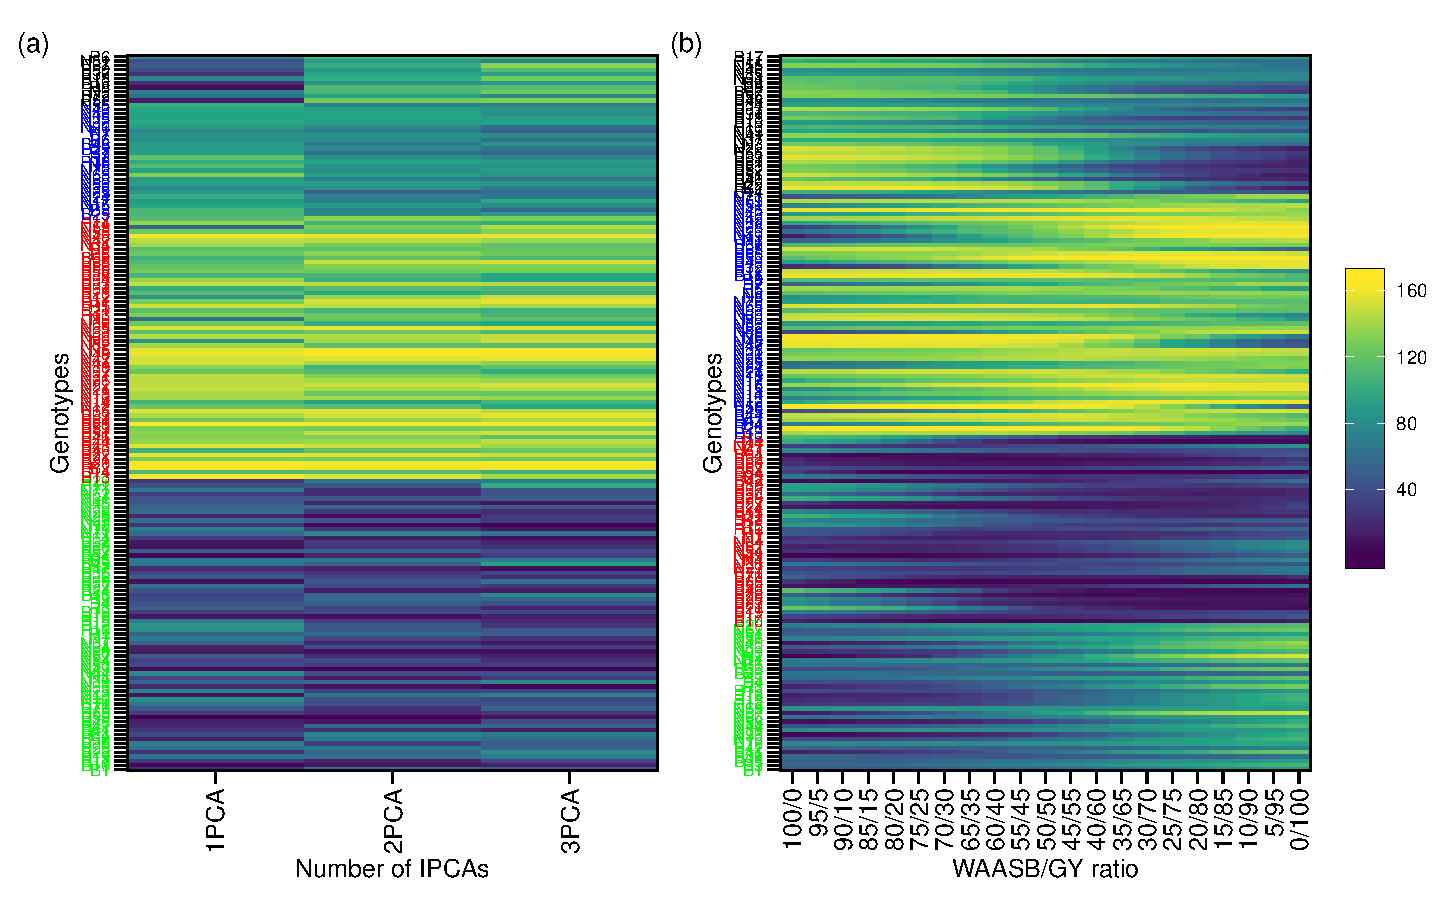
\includegraphics{figures/mod metan all_mkt stab6-1} \end{center}

\hypertarget{coincidence-index-of-genotype-selection}{%
\paragraph{Coincidence index of genotype
selection}\label{coincidence-index-of-genotype-selection}}

Computes the coincidence index (Hamblin and Zimmermann, 1986) as
follows:

\[
{CI = \frac{A-C}{M-C}\times 100}
\]

where \emph{A} is the number of selected genotypes common to different
methods; \emph{C} is the number of expected genotypes selected by
chance; and \emph{M} is the number of genotypes selected according to
the selection intensity.

\begin{Shaded}
\begin{Highlighting}[]
\NormalTok{coinc\_1 }\OtherTok{\textless{}{-}}\NormalTok{ stab\_blups }\SpecialCharTok{\%\textgreater{}\%}\NormalTok{ dplyr}\SpecialCharTok{::}\FunctionTok{select}\NormalTok{(GEN,HMRPGV\_R) }\SpecialCharTok{\%\textgreater{}\%} \FunctionTok{arrange}\NormalTok{(HMRPGV\_R)}
\NormalTok{coinc\_2 }\OtherTok{\textless{}{-}}\NormalTok{ stab\_blups }\SpecialCharTok{\%\textgreater{}\%}\NormalTok{ dplyr}\SpecialCharTok{::}\FunctionTok{select}\NormalTok{(GEN,RPGV\_R) }\SpecialCharTok{\%\textgreater{}\%} \FunctionTok{arrange}\NormalTok{(RPGV\_R)}
\NormalTok{coinc\_3 }\OtherTok{\textless{}{-}}\NormalTok{ stab\_blups }\SpecialCharTok{\%\textgreater{}\%}\NormalTok{ dplyr}\SpecialCharTok{::}\FunctionTok{select}\NormalTok{(GEN,HMGV\_R) }\SpecialCharTok{\%\textgreater{}\%} \FunctionTok{arrange}\NormalTok{(HMGV\_R)}
\NormalTok{coinc\_4 }\OtherTok{\textless{}{-}}\NormalTok{ stab\_blups }\SpecialCharTok{\%\textgreater{}\%}\NormalTok{ dplyr}\SpecialCharTok{::}\FunctionTok{select}\NormalTok{(GEN,OrWAASBY) }\SpecialCharTok{\%\textgreater{}\%} \FunctionTok{arrange}\NormalTok{(OrWAASBY)}
\NormalTok{coinc\_5 }\OtherTok{\textless{}{-}}\NormalTok{ stab\_blups }\SpecialCharTok{\%\textgreater{}\%}\NormalTok{ dplyr}\SpecialCharTok{::}\FunctionTok{select}\NormalTok{(GEN,WAASB\_R) }\SpecialCharTok{\%\textgreater{}\%} \FunctionTok{arrange}\NormalTok{(WAASB\_R)}

\NormalTok{selc\_perc}\OtherTok{\textless{}{-}} \FunctionTok{round}\NormalTok{(}\FunctionTok{nrow}\NormalTok{(stab\_blups)}\SpecialCharTok{*}\FloatTok{0.2}\NormalTok{)}

\NormalTok{coinc\_1}\FloatTok{.1} \OtherTok{\textless{}{-}}\DecValTok{1}
\NormalTok{coinc\_1}\FloatTok{.2} \OtherTok{\textless{}{-}} \FunctionTok{coincidence\_index}\NormalTok{(}\AttributeTok{sel1 =}\NormalTok{ coinc\_1}\SpecialCharTok{$}\NormalTok{GEN[}\DecValTok{1}\SpecialCharTok{:}\NormalTok{selc\_perc], }
                                        \AttributeTok{sel2 =}\NormalTok{ coinc\_2}\SpecialCharTok{$}\NormalTok{GEN[}\DecValTok{1}\SpecialCharTok{:}\NormalTok{selc\_perc], }
                                        \AttributeTok{total =} \DecValTok{72}\NormalTok{)}\SpecialCharTok{/}\DecValTok{100}
\NormalTok{coinc\_1}\FloatTok{.3} \OtherTok{\textless{}{-}} \FunctionTok{coincidence\_index}\NormalTok{(}\AttributeTok{sel1 =}\NormalTok{ coinc\_1}\SpecialCharTok{$}\NormalTok{GEN[}\DecValTok{1}\SpecialCharTok{:}\NormalTok{selc\_perc], }
                                        \AttributeTok{sel2 =}\NormalTok{ coinc\_3}\SpecialCharTok{$}\NormalTok{GEN[}\DecValTok{1}\SpecialCharTok{:}\NormalTok{selc\_perc], }
                                        \AttributeTok{total =} \DecValTok{72}\NormalTok{)}\SpecialCharTok{/}\DecValTok{100}
\NormalTok{coinc\_1}\FloatTok{.4} \OtherTok{\textless{}{-}} \FunctionTok{coincidence\_index}\NormalTok{(}\AttributeTok{sel1 =}\NormalTok{ coinc\_1}\SpecialCharTok{$}\NormalTok{GEN[}\DecValTok{1}\SpecialCharTok{:}\NormalTok{selc\_perc], }
                                        \AttributeTok{sel2 =}\NormalTok{ coinc\_4}\SpecialCharTok{$}\NormalTok{GEN[}\DecValTok{1}\SpecialCharTok{:}\NormalTok{selc\_perc], }
                                        \AttributeTok{total =} \DecValTok{72}\NormalTok{)}\SpecialCharTok{/}\DecValTok{100}
\NormalTok{coinc\_1}\FloatTok{.5} \OtherTok{\textless{}{-}} \FunctionTok{coincidence\_index}\NormalTok{(}\AttributeTok{sel1 =}\NormalTok{ coinc\_1}\SpecialCharTok{$}\NormalTok{GEN[}\DecValTok{1}\SpecialCharTok{:}\NormalTok{selc\_perc], }
                                        \AttributeTok{sel2 =}\NormalTok{ coinc\_5}\SpecialCharTok{$}\NormalTok{GEN[}\DecValTok{1}\SpecialCharTok{:}\NormalTok{selc\_perc], }
                                        \AttributeTok{total =} \DecValTok{72}\NormalTok{)}\SpecialCharTok{/}\DecValTok{100}
\NormalTok{coinc\_2}\FloatTok{.2} \OtherTok{\textless{}{-}}\DecValTok{1}
\NormalTok{coinc\_2}\FloatTok{.3} \OtherTok{\textless{}{-}} \FunctionTok{coincidence\_index}\NormalTok{(}\AttributeTok{sel1 =}\NormalTok{ coinc\_2}\SpecialCharTok{$}\NormalTok{GEN[}\DecValTok{1}\SpecialCharTok{:}\NormalTok{selc\_perc], }
                                        \AttributeTok{sel2 =}\NormalTok{ coinc\_3}\SpecialCharTok{$}\NormalTok{GEN[}\DecValTok{1}\SpecialCharTok{:}\NormalTok{selc\_perc], }
                                        \AttributeTok{total =} \DecValTok{72}\NormalTok{)}\SpecialCharTok{/}\DecValTok{100}
\NormalTok{coinc\_2}\FloatTok{.4} \OtherTok{\textless{}{-}} \FunctionTok{coincidence\_index}\NormalTok{(}\AttributeTok{sel1 =}\NormalTok{ coinc\_2}\SpecialCharTok{$}\NormalTok{GEN[}\DecValTok{1}\SpecialCharTok{:}\NormalTok{selc\_perc], }
                                        \AttributeTok{sel2 =}\NormalTok{ coinc\_4}\SpecialCharTok{$}\NormalTok{GEN[}\DecValTok{1}\SpecialCharTok{:}\NormalTok{selc\_perc], }
                                        \AttributeTok{total =} \DecValTok{72}\NormalTok{)}\SpecialCharTok{/}\DecValTok{100}
\NormalTok{coinc\_2}\FloatTok{.5} \OtherTok{\textless{}{-}} \FunctionTok{coincidence\_index}\NormalTok{(}\AttributeTok{sel1 =}\NormalTok{ coinc\_2}\SpecialCharTok{$}\NormalTok{GEN[}\DecValTok{1}\SpecialCharTok{:}\NormalTok{selc\_perc], }
                                        \AttributeTok{sel2 =}\NormalTok{ coinc\_5}\SpecialCharTok{$}\NormalTok{GEN[}\DecValTok{1}\SpecialCharTok{:}\NormalTok{selc\_perc], }
                                        \AttributeTok{total =} \DecValTok{72}\NormalTok{)}\SpecialCharTok{/}\DecValTok{100}
\NormalTok{coinc\_3}\FloatTok{.3}\OtherTok{\textless{}{-}} \DecValTok{1}
\NormalTok{coinc\_3}\FloatTok{.4} \OtherTok{\textless{}{-}} \FunctionTok{coincidence\_index}\NormalTok{(}\AttributeTok{sel1 =}\NormalTok{ coinc\_3}\SpecialCharTok{$}\NormalTok{GEN[}\DecValTok{1}\SpecialCharTok{:}\NormalTok{selc\_perc], }
                                        \AttributeTok{sel2 =}\NormalTok{ coinc\_4}\SpecialCharTok{$}\NormalTok{GEN[}\DecValTok{1}\SpecialCharTok{:}\NormalTok{selc\_perc], }
                                        \AttributeTok{total =} \DecValTok{72}\NormalTok{)}\SpecialCharTok{/}\DecValTok{100}
\NormalTok{coinc\_3}\FloatTok{.5} \OtherTok{\textless{}{-}} \FunctionTok{coincidence\_index}\NormalTok{(}\AttributeTok{sel1 =}\NormalTok{ coinc\_3}\SpecialCharTok{$}\NormalTok{GEN[}\DecValTok{1}\SpecialCharTok{:}\NormalTok{selc\_perc], }
                                        \AttributeTok{sel2 =}\NormalTok{ coinc\_5}\SpecialCharTok{$}\NormalTok{GEN[}\DecValTok{1}\SpecialCharTok{:}\NormalTok{selc\_perc], }
                                        \AttributeTok{total =} \DecValTok{72}\NormalTok{)}\SpecialCharTok{/}\DecValTok{100}
\NormalTok{coinc\_4}\FloatTok{.4} \OtherTok{\textless{}{-}} \DecValTok{1}
\NormalTok{coinc\_4}\FloatTok{.5} \OtherTok{\textless{}{-}} \FunctionTok{coincidence\_index}\NormalTok{(}\AttributeTok{sel1 =}\NormalTok{ coinc\_4}\SpecialCharTok{$}\NormalTok{GEN[}\DecValTok{1}\SpecialCharTok{:}\NormalTok{selc\_perc], }
                                        \AttributeTok{sel2 =}\NormalTok{ coinc\_5}\SpecialCharTok{$}\NormalTok{GEN[}\DecValTok{1}\SpecialCharTok{:}\NormalTok{selc\_perc], }
                                        \AttributeTok{total =} \DecValTok{72}\NormalTok{)}\SpecialCharTok{/}\DecValTok{100}
\NormalTok{coinc\_5}\FloatTok{.5} \OtherTok{\textless{}{-}} \DecValTok{1}


\NormalTok{coinc}\OtherTok{\textless{}{-}} \FunctionTok{c}\NormalTok{(coinc\_1}\FloatTok{.1}\NormalTok{,coinc\_1}\FloatTok{.2}\NormalTok{,coinc\_2}\FloatTok{.2}\NormalTok{,coinc\_1}\FloatTok{.3}\NormalTok{,coinc\_2}\FloatTok{.3}\NormalTok{,}
\NormalTok{          coinc\_3}\FloatTok{.3}\NormalTok{,coinc\_1}\FloatTok{.4}\NormalTok{, coinc\_2}\FloatTok{.4}\NormalTok{, coinc\_3}\FloatTok{.4}\NormalTok{,}
\NormalTok{          coinc\_4}\FloatTok{.4}\NormalTok{, coinc\_1}\FloatTok{.5}\NormalTok{, coinc\_2}\FloatTok{.5}\NormalTok{,}
\NormalTok{          coinc\_3}\FloatTok{.5}\NormalTok{, coinc\_4}\FloatTok{.5}\NormalTok{,}
\NormalTok{          coinc\_5}\FloatTok{.5}\NormalTok{)}
  
\NormalTok{z}\OtherTok{=}\FunctionTok{matrix}\NormalTok{(}\DecValTok{0}\NormalTok{,}\DecValTok{5}\NormalTok{,}\DecValTok{5}\NormalTok{)}
\NormalTok{z[}\FunctionTok{upper.tri}\NormalTok{(z)}\SpecialCharTok{|} \FunctionTok{row}\NormalTok{(z)}\SpecialCharTok{==}\FunctionTok{col}\NormalTok{(z)] }\OtherTok{\textless{}{-}}\NormalTok{ coinc}

\FunctionTok{rownames}\NormalTok{(z)}\OtherTok{=}\FunctionTok{c}\NormalTok{(}
\StringTok{"HMRPGV"}\NormalTok{,}
\StringTok{"RPGV"}\NormalTok{,}
\StringTok{\textquotesingle{}HMGV\textquotesingle{}}\NormalTok{,}
\StringTok{\textquotesingle{}WAASBY\textquotesingle{}}\NormalTok{,}
\StringTok{\textquotesingle{}WAASB\textquotesingle{}}\NormalTok{)}

\FunctionTok{colnames}\NormalTok{(z)}\OtherTok{=}\FunctionTok{rownames}\NormalTok{(z)}

\NormalTok{plot}\OtherTok{\textless{}{-}} \FunctionTok{ggcorrplot}\NormalTok{(z, }\AttributeTok{colors =} \FunctionTok{c}\NormalTok{(}\StringTok{"\#6D9EC1"}\NormalTok{, }\StringTok{"gray"}\NormalTok{ ,}\StringTok{"\#E46726"}\NormalTok{),  }
           \AttributeTok{show.legend =}\NormalTok{ T,}
\AttributeTok{legend.title =} \StringTok{"CI"}\NormalTok{ ,}\AttributeTok{lab\_size=}\DecValTok{5}\NormalTok{,}\AttributeTok{tl.srt =} \DecValTok{90}\NormalTok{,}\AttributeTok{type =} \FunctionTok{c}\NormalTok{(}\StringTok{"upper"}\NormalTok{), }\AttributeTok{lab =}\NormalTok{ T,}\AttributeTok{digits =} \DecValTok{4}\NormalTok{,}
\AttributeTok{outline.color =} \StringTok{"white"}\NormalTok{,}\AttributeTok{pch.col =} \StringTok{"white"}\NormalTok{, }\AttributeTok{tl.col =} \StringTok{"blue"}\NormalTok{,}\AttributeTok{show.diag =}\NormalTok{ F) }\SpecialCharTok{+}
  \FunctionTok{labs}\NormalTok{(}\AttributeTok{title =} \StringTok{"BLUP{-}based stability indexes coincidence across all market classes"}\NormalTok{,}
           \AttributeTok{subtitle =} \StringTok{"Selection intensity of 20\% top genotypes"}\NormalTok{)}

\FunctionTok{print}\NormalTok{(plot)}
\end{Highlighting}
\end{Shaded}

\begin{center}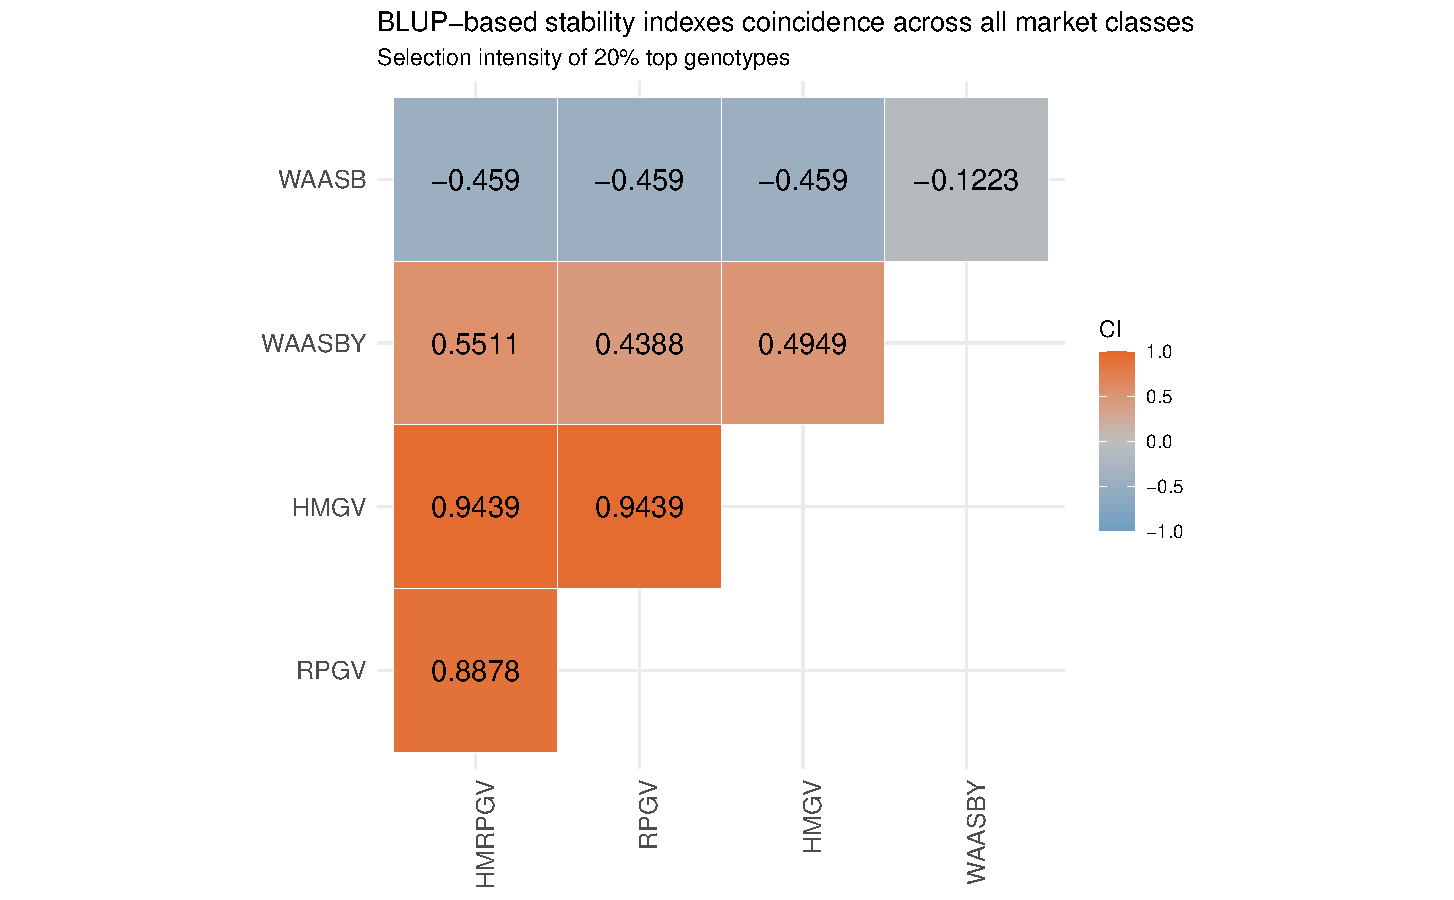
\includegraphics{figures/mod metan stab7-1} \end{center}

\hypertarget{met-analysis---black-beans}{%
\subsection{\texorpdfstring{MET analysis - \textbf{Black
beans}}{MET analysis - Black beans}}\label{met-analysis---black-beans}}

\hypertarget{met-analysis---asreml-1}{%
\subsubsection{MET analysis - ASReml}\label{met-analysis---asreml-1}}

Running MET using \texttt{ASReml} - only to comparison of variance
components with \texttt{metan} outputs

\begin{Shaded}
\begin{Highlighting}[]
\NormalTok{mod.met.asreml.bb1 }\OtherTok{\textless{}{-}} \FunctionTok{asreml}\NormalTok{(}\AttributeTok{fixed       =}\NormalTok{ yield }\SpecialCharTok{\textasciitilde{}}\NormalTok{  loc }\SpecialCharTok{+}\NormalTok{ loc}\SpecialCharTok{:}\NormalTok{rep,}
                     \AttributeTok{random      =} \SpecialCharTok{\textasciitilde{}}\NormalTok{  name }\SpecialCharTok{+}\NormalTok{ name}\SpecialCharTok{:}\NormalTok{loc,}
                     \AttributeTok{data        =}\NormalTok{ blues\_stage.I\_BB,}
                     \AttributeTok{predict     =} \FunctionTok{predict.asreml}\NormalTok{(}\AttributeTok{classify =} \StringTok{"name"}\NormalTok{),}
                     \AttributeTok{trace       =}\NormalTok{ F,}
                     \AttributeTok{maxit       =} \DecValTok{500}\NormalTok{)}

\NormalTok{summFix.bb.met.asreml}\OtherTok{\textless{}{-}} \FunctionTok{data.frame}\NormalTok{(}\FunctionTok{wald}\NormalTok{(mod.met.asreml.bb1))}
\NormalTok{summFix.bb.met.asreml}
\end{Highlighting}
\end{Shaded}

\global\setlength{\Oldarrayrulewidth}{\arrayrulewidth}

\global\setlength{\Oldtabcolsep}{\tabcolsep}

\setlength{\tabcolsep}{0pt}

\renewcommand*{\arraystretch}{1.5}



\providecommand{\ascline}[3]{\noalign{\global\arrayrulewidth #1}\arrayrulecolor[HTML]{#2}\cline{#3}}

\begin{longtable}[c]{|p{0.75in}|p{1.01in}|p{1.02in}|p{0.76in}}



\ascline{1.5pt}{666666}{1-4}

\multicolumn{1}{>{\raggedleft}m{\dimexpr 0.75in+0\tabcolsep}}{\textcolor[HTML]{000000}{\fontsize{9}{9}\selectfont{\global\setmainfont{Arial}{\textbf{Df}}}}} & \multicolumn{1}{>{\raggedleft}m{\dimexpr 1.01in+0\tabcolsep}}{\textcolor[HTML]{000000}{\fontsize{9}{9}\selectfont{\global\setmainfont{Arial}{\textbf{Sum.of.Sq}}}}} & \multicolumn{1}{>{\raggedleft}m{\dimexpr 1.02in+0\tabcolsep}}{\textcolor[HTML]{000000}{\fontsize{9}{9}\selectfont{\global\setmainfont{Arial}{\textbf{Wald.statistic}}}}} & \multicolumn{1}{>{\raggedleft}m{\dimexpr 0.76in+0\tabcolsep}}{\textcolor[HTML]{000000}{\fontsize{9}{9}\selectfont{\global\setmainfont{Arial}{\textbf{Pr.Chisq.}}}}} \\

\ascline{0.75pt}{666666}{1-4}



\multicolumn{1}{>{\raggedleft}m{\dimexpr 0.75in+0\tabcolsep}}{\textcolor[HTML]{999999}{\fontsize{9}{9}\selectfont{\global\setmainfont{Arial}{\textbf{numeric}}}}} & \multicolumn{1}{>{\raggedleft}m{\dimexpr 1.01in+0\tabcolsep}}{\textcolor[HTML]{999999}{\fontsize{9}{9}\selectfont{\global\setmainfont{Arial}{\textbf{numeric}}}}} & \multicolumn{1}{>{\raggedleft}m{\dimexpr 1.02in+0\tabcolsep}}{\textcolor[HTML]{999999}{\fontsize{9}{9}\selectfont{\global\setmainfont{Arial}{\textbf{numeric}}}}} & \multicolumn{1}{>{\raggedleft}m{\dimexpr 0.76in+0\tabcolsep}}{\textcolor[HTML]{999999}{\fontsize{9}{9}\selectfont{\global\setmainfont{Arial}{\textbf{numeric}}}}} \\

\ascline{1.5pt}{666666}{1-4}\endfirsthead

\ascline{1.5pt}{666666}{1-4}

\multicolumn{1}{>{\raggedleft}m{\dimexpr 0.75in+0\tabcolsep}}{\textcolor[HTML]{000000}{\fontsize{9}{9}\selectfont{\global\setmainfont{Arial}{\textbf{Df}}}}} & \multicolumn{1}{>{\raggedleft}m{\dimexpr 1.01in+0\tabcolsep}}{\textcolor[HTML]{000000}{\fontsize{9}{9}\selectfont{\global\setmainfont{Arial}{\textbf{Sum.of.Sq}}}}} & \multicolumn{1}{>{\raggedleft}m{\dimexpr 1.02in+0\tabcolsep}}{\textcolor[HTML]{000000}{\fontsize{9}{9}\selectfont{\global\setmainfont{Arial}{\textbf{Wald.statistic}}}}} & \multicolumn{1}{>{\raggedleft}m{\dimexpr 0.76in+0\tabcolsep}}{\textcolor[HTML]{000000}{\fontsize{9}{9}\selectfont{\global\setmainfont{Arial}{\textbf{Pr.Chisq.}}}}} \\

\ascline{0.75pt}{666666}{1-4}



\multicolumn{1}{>{\raggedleft}m{\dimexpr 0.75in+0\tabcolsep}}{\textcolor[HTML]{999999}{\fontsize{9}{9}\selectfont{\global\setmainfont{Arial}{\textbf{numeric}}}}} & \multicolumn{1}{>{\raggedleft}m{\dimexpr 1.01in+0\tabcolsep}}{\textcolor[HTML]{999999}{\fontsize{9}{9}\selectfont{\global\setmainfont{Arial}{\textbf{numeric}}}}} & \multicolumn{1}{>{\raggedleft}m{\dimexpr 1.02in+0\tabcolsep}}{\textcolor[HTML]{999999}{\fontsize{9}{9}\selectfont{\global\setmainfont{Arial}{\textbf{numeric}}}}} & \multicolumn{1}{>{\raggedleft}m{\dimexpr 0.76in+0\tabcolsep}}{\textcolor[HTML]{999999}{\fontsize{9}{9}\selectfont{\global\setmainfont{Arial}{\textbf{numeric}}}}} \\

\ascline{1.5pt}{666666}{1-4}\endhead



\multicolumn{4}{>{\raggedleft}m{\dimexpr 3.54in+6\tabcolsep}}{\textcolor[HTML]{000000}{\fontsize{9}{9}\selectfont{\global\setmainfont{Arial}{n:\ 4}}}} \\

\ascline{0.75pt}{666666}{1-4}\endfoot



\multicolumn{1}{>{\raggedleft}m{\dimexpr 0.75in+0\tabcolsep}}{\textcolor[HTML]{000000}{\fontsize{9}{9}\selectfont{\global\setmainfont{Arial}{1}}}} & \multicolumn{1}{>{\raggedleft}m{\dimexpr 1.01in+0\tabcolsep}}{\textcolor[HTML]{000000}{\fontsize{9}{9}\selectfont{\global\setmainfont{Arial}{1,368,373,852}}}} & \multicolumn{1}{>{\raggedleft}m{\dimexpr 1.02in+0\tabcolsep}}{\textcolor[HTML]{000000}{\fontsize{9}{9}\selectfont{\global\setmainfont{Arial}{7,427.1}}}} & \multicolumn{1}{>{\raggedleft}m{\dimexpr 0.76in+0\tabcolsep}}{\textcolor[HTML]{000000}{\fontsize{9}{9}\selectfont{\global\setmainfont{Arial}{0}}}} \\

\ascline{0.75pt}{666666}{1-4}



\multicolumn{1}{>{\raggedleft}m{\dimexpr 0.75in+0\tabcolsep}}{\textcolor[HTML]{000000}{\fontsize{9}{9}\selectfont{\global\setmainfont{Arial}{3}}}} & \multicolumn{1}{>{\raggedleft}m{\dimexpr 1.01in+0\tabcolsep}}{\textcolor[HTML]{000000}{\fontsize{9}{9}\selectfont{\global\setmainfont{Arial}{7,396,784}}}} & \multicolumn{1}{>{\raggedleft}m{\dimexpr 1.02in+0\tabcolsep}}{\textcolor[HTML]{000000}{\fontsize{9}{9}\selectfont{\global\setmainfont{Arial}{40.1}}}} & \multicolumn{1}{>{\raggedleft}m{\dimexpr 0.76in+0\tabcolsep}}{\textcolor[HTML]{000000}{\fontsize{9}{9}\selectfont{\global\setmainfont{Arial}{0}}}} \\

\ascline{0.75pt}{666666}{1-4}



\multicolumn{1}{>{\raggedleft}m{\dimexpr 0.75in+0\tabcolsep}}{\textcolor[HTML]{000000}{\fontsize{9}{9}\selectfont{\global\setmainfont{Arial}{12}}}} & \multicolumn{1}{>{\raggedleft}m{\dimexpr 1.01in+0\tabcolsep}}{\textcolor[HTML]{000000}{\fontsize{9}{9}\selectfont{\global\setmainfont{Arial}{21,308,617}}}} & \multicolumn{1}{>{\raggedleft}m{\dimexpr 1.02in+0\tabcolsep}}{\textcolor[HTML]{000000}{\fontsize{9}{9}\selectfont{\global\setmainfont{Arial}{115.7}}}} & \multicolumn{1}{>{\raggedleft}m{\dimexpr 0.76in+0\tabcolsep}}{\textcolor[HTML]{000000}{\fontsize{9}{9}\selectfont{\global\setmainfont{Arial}{0}}}} \\

\ascline{0.75pt}{666666}{1-4}



\multicolumn{1}{>{\raggedleft}m{\dimexpr 0.75in+0\tabcolsep}}{\textcolor[HTML]{000000}{\fontsize{9}{9}\selectfont{\global\setmainfont{Arial}{}}}} & \multicolumn{1}{>{\raggedleft}m{\dimexpr 1.01in+0\tabcolsep}}{\textcolor[HTML]{000000}{\fontsize{9}{9}\selectfont{\global\setmainfont{Arial}{184,240}}}} & \multicolumn{1}{>{\raggedleft}m{\dimexpr 1.02in+0\tabcolsep}}{\textcolor[HTML]{000000}{\fontsize{9}{9}\selectfont{\global\setmainfont{Arial}{}}}} & \multicolumn{1}{>{\raggedleft}m{\dimexpr 0.76in+0\tabcolsep}}{\textcolor[HTML]{000000}{\fontsize{9}{9}\selectfont{\global\setmainfont{Arial}{}}}} \\

\ascline{1.5pt}{666666}{1-4}



\end{longtable}



\arrayrulecolor[HTML]{000000}

\global\setlength{\arrayrulewidth}{\Oldarrayrulewidth}

\global\setlength{\tabcolsep}{\Oldtabcolsep}

\renewcommand*{\arraystretch}{1}

\begin{Shaded}
\begin{Highlighting}[]
\NormalTok{summ.bb.met.asreml}\OtherTok{\textless{}{-}} \FunctionTok{data.frame}\NormalTok{(}\FunctionTok{summary.asreml}\NormalTok{(mod.met.asreml.bb1)}\SpecialCharTok{$}\NormalTok{varcomp)}
\NormalTok{summ.bb.met.asreml}
\end{Highlighting}
\end{Shaded}

\global\setlength{\Oldarrayrulewidth}{\arrayrulewidth}

\global\setlength{\Oldtabcolsep}{\tabcolsep}

\setlength{\tabcolsep}{0pt}

\renewcommand*{\arraystretch}{1.5}



\providecommand{\ascline}[3]{\noalign{\global\arrayrulewidth #1}\arrayrulecolor[HTML]{#2}\cline{#3}}

\begin{longtable}[c]{|p{0.88in}|p{0.75in}|p{0.75in}|p{0.77in}|p{0.75in}}



\ascline{1.5pt}{666666}{1-5}

\multicolumn{1}{>{\raggedleft}m{\dimexpr 0.88in+0\tabcolsep}}{\textcolor[HTML]{000000}{\fontsize{9}{9}\selectfont{\global\setmainfont{Arial}{\textbf{component}}}}} & \multicolumn{1}{>{\raggedleft}m{\dimexpr 0.75in+0\tabcolsep}}{\textcolor[HTML]{000000}{\fontsize{9}{9}\selectfont{\global\setmainfont{Arial}{\textbf{std.error}}}}} & \multicolumn{1}{>{\raggedleft}m{\dimexpr 0.75in+0\tabcolsep}}{\textcolor[HTML]{000000}{\fontsize{9}{9}\selectfont{\global\setmainfont{Arial}{\textbf{z.ratio}}}}} & \multicolumn{1}{>{\raggedright}m{\dimexpr 0.77in+0\tabcolsep}}{\textcolor[HTML]{000000}{\fontsize{9}{9}\selectfont{\global\setmainfont{Arial}{\textbf{bound}}}}} & \multicolumn{1}{>{\raggedleft}m{\dimexpr 0.75in+0\tabcolsep}}{\textcolor[HTML]{000000}{\fontsize{9}{9}\selectfont{\global\setmainfont{Arial}{\textbf{X.ch}}}}} \\

\ascline{0.75pt}{666666}{1-5}



\multicolumn{1}{>{\raggedleft}m{\dimexpr 0.88in+0\tabcolsep}}{\textcolor[HTML]{999999}{\fontsize{9}{9}\selectfont{\global\setmainfont{Arial}{\textbf{numeric}}}}} & \multicolumn{1}{>{\raggedleft}m{\dimexpr 0.75in+0\tabcolsep}}{\textcolor[HTML]{999999}{\fontsize{9}{9}\selectfont{\global\setmainfont{Arial}{\textbf{numeric}}}}} & \multicolumn{1}{>{\raggedleft}m{\dimexpr 0.75in+0\tabcolsep}}{\textcolor[HTML]{999999}{\fontsize{9}{9}\selectfont{\global\setmainfont{Arial}{\textbf{numeric}}}}} & \multicolumn{1}{>{\raggedright}m{\dimexpr 0.77in+0\tabcolsep}}{\textcolor[HTML]{999999}{\fontsize{9}{9}\selectfont{\global\setmainfont{Arial}{\textbf{character}}}}} & \multicolumn{1}{>{\raggedleft}m{\dimexpr 0.75in+0\tabcolsep}}{\textcolor[HTML]{999999}{\fontsize{9}{9}\selectfont{\global\setmainfont{Arial}{\textbf{numeric}}}}} \\

\ascline{1.5pt}{666666}{1-5}\endfirsthead

\ascline{1.5pt}{666666}{1-5}

\multicolumn{1}{>{\raggedleft}m{\dimexpr 0.88in+0\tabcolsep}}{\textcolor[HTML]{000000}{\fontsize{9}{9}\selectfont{\global\setmainfont{Arial}{\textbf{component}}}}} & \multicolumn{1}{>{\raggedleft}m{\dimexpr 0.75in+0\tabcolsep}}{\textcolor[HTML]{000000}{\fontsize{9}{9}\selectfont{\global\setmainfont{Arial}{\textbf{std.error}}}}} & \multicolumn{1}{>{\raggedleft}m{\dimexpr 0.75in+0\tabcolsep}}{\textcolor[HTML]{000000}{\fontsize{9}{9}\selectfont{\global\setmainfont{Arial}{\textbf{z.ratio}}}}} & \multicolumn{1}{>{\raggedright}m{\dimexpr 0.77in+0\tabcolsep}}{\textcolor[HTML]{000000}{\fontsize{9}{9}\selectfont{\global\setmainfont{Arial}{\textbf{bound}}}}} & \multicolumn{1}{>{\raggedleft}m{\dimexpr 0.75in+0\tabcolsep}}{\textcolor[HTML]{000000}{\fontsize{9}{9}\selectfont{\global\setmainfont{Arial}{\textbf{X.ch}}}}} \\

\ascline{0.75pt}{666666}{1-5}



\multicolumn{1}{>{\raggedleft}m{\dimexpr 0.88in+0\tabcolsep}}{\textcolor[HTML]{999999}{\fontsize{9}{9}\selectfont{\global\setmainfont{Arial}{\textbf{numeric}}}}} & \multicolumn{1}{>{\raggedleft}m{\dimexpr 0.75in+0\tabcolsep}}{\textcolor[HTML]{999999}{\fontsize{9}{9}\selectfont{\global\setmainfont{Arial}{\textbf{numeric}}}}} & \multicolumn{1}{>{\raggedleft}m{\dimexpr 0.75in+0\tabcolsep}}{\textcolor[HTML]{999999}{\fontsize{9}{9}\selectfont{\global\setmainfont{Arial}{\textbf{numeric}}}}} & \multicolumn{1}{>{\raggedright}m{\dimexpr 0.77in+0\tabcolsep}}{\textcolor[HTML]{999999}{\fontsize{9}{9}\selectfont{\global\setmainfont{Arial}{\textbf{character}}}}} & \multicolumn{1}{>{\raggedleft}m{\dimexpr 0.75in+0\tabcolsep}}{\textcolor[HTML]{999999}{\fontsize{9}{9}\selectfont{\global\setmainfont{Arial}{\textbf{numeric}}}}} \\

\ascline{1.5pt}{666666}{1-5}\endhead



\multicolumn{5}{>{\raggedleft}m{\dimexpr 3.91in+8\tabcolsep}}{\textcolor[HTML]{000000}{\fontsize{9}{9}\selectfont{\global\setmainfont{Arial}{n:\ 3}}}} \\

\ascline{0.75pt}{666666}{1-5}\endfoot



\multicolumn{1}{>{\raggedleft}m{\dimexpr 0.88in+0\tabcolsep}}{\textcolor[HTML]{000000}{\fontsize{9}{9}\selectfont{\global\setmainfont{Arial}{48,605.0}}}} & \multicolumn{1}{>{\raggedleft}m{\dimexpr 0.75in+0\tabcolsep}}{\textcolor[HTML]{000000}{\fontsize{9}{9}\selectfont{\global\setmainfont{Arial}{17,987.9}}}} & \multicolumn{1}{>{\raggedleft}m{\dimexpr 0.75in+0\tabcolsep}}{\textcolor[HTML]{000000}{\fontsize{9}{9}\selectfont{\global\setmainfont{Arial}{2.7}}}} & \multicolumn{1}{>{\raggedright}m{\dimexpr 0.77in+0\tabcolsep}}{\textcolor[HTML]{000000}{\fontsize{9}{9}\selectfont{\global\setmainfont{Arial}{P}}}} & \multicolumn{1}{>{\raggedleft}m{\dimexpr 0.75in+0\tabcolsep}}{\textcolor[HTML]{000000}{\fontsize{9}{9}\selectfont{\global\setmainfont{Arial}{0}}}} \\

\ascline{0.75pt}{666666}{1-5}



\multicolumn{1}{>{\raggedleft}m{\dimexpr 0.88in+0\tabcolsep}}{\textcolor[HTML]{000000}{\fontsize{9}{9}\selectfont{\global\setmainfont{Arial}{164,940.6}}}} & \multicolumn{1}{>{\raggedleft}m{\dimexpr 0.75in+0\tabcolsep}}{\textcolor[HTML]{000000}{\fontsize{9}{9}\selectfont{\global\setmainfont{Arial}{21,008.6}}}} & \multicolumn{1}{>{\raggedleft}m{\dimexpr 0.75in+0\tabcolsep}}{\textcolor[HTML]{000000}{\fontsize{9}{9}\selectfont{\global\setmainfont{Arial}{7.9}}}} & \multicolumn{1}{>{\raggedright}m{\dimexpr 0.77in+0\tabcolsep}}{\textcolor[HTML]{000000}{\fontsize{9}{9}\selectfont{\global\setmainfont{Arial}{P}}}} & \multicolumn{1}{>{\raggedleft}m{\dimexpr 0.75in+0\tabcolsep}}{\textcolor[HTML]{000000}{\fontsize{9}{9}\selectfont{\global\setmainfont{Arial}{0}}}} \\

\ascline{0.75pt}{666666}{1-5}



\multicolumn{1}{>{\raggedleft}m{\dimexpr 0.88in+0\tabcolsep}}{\textcolor[HTML]{000000}{\fontsize{9}{9}\selectfont{\global\setmainfont{Arial}{184,240.9}}}} & \multicolumn{1}{>{\raggedleft}m{\dimexpr 0.75in+0\tabcolsep}}{\textcolor[HTML]{000000}{\fontsize{9}{9}\selectfont{\global\setmainfont{Arial}{9,279.9}}}} & \multicolumn{1}{>{\raggedleft}m{\dimexpr 0.75in+0\tabcolsep}}{\textcolor[HTML]{000000}{\fontsize{9}{9}\selectfont{\global\setmainfont{Arial}{19.9}}}} & \multicolumn{1}{>{\raggedright}m{\dimexpr 0.77in+0\tabcolsep}}{\textcolor[HTML]{000000}{\fontsize{9}{9}\selectfont{\global\setmainfont{Arial}{P}}}} & \multicolumn{1}{>{\raggedleft}m{\dimexpr 0.75in+0\tabcolsep}}{\textcolor[HTML]{000000}{\fontsize{9}{9}\selectfont{\global\setmainfont{Arial}{0}}}} \\

\ascline{1.5pt}{666666}{1-5}



\end{longtable}



\arrayrulecolor[HTML]{000000}

\global\setlength{\arrayrulewidth}{\Oldarrayrulewidth}

\global\setlength{\tabcolsep}{\Oldtabcolsep}

\renewcommand*{\arraystretch}{1}

\begin{Shaded}
\begin{Highlighting}[]
\CommentTok{\#print(summary.asreml(mod.met.asreml.bb1)$bic)}
\NormalTok{mod.met.asreml.bb}\OtherTok{\textless{}{-}} \FunctionTok{as.data.frame}\NormalTok{((mod.met.asreml.bb1}\SpecialCharTok{$}\NormalTok{predictions}\SpecialCharTok{$}\NormalTok{pvals[}\DecValTok{1}\SpecialCharTok{:}\DecValTok{3}\NormalTok{]))}
\FunctionTok{names}\NormalTok{(mod.met.asreml.bb) }\OtherTok{\textless{}{-}} \FunctionTok{c}\NormalTok{(}\StringTok{"name"}\NormalTok{, }\StringTok{"yield\_BLUPS\_MET"}\NormalTok{, }\StringTok{"SE"}\NormalTok{)}

\DocumentationTok{\#\#\#}
\end{Highlighting}
\end{Shaded}

\hypertarget{met-analysis---lme4-1}{%
\subsubsection{MET analysis - lme4}\label{met-analysis---lme4-1}}

Running MET using \texttt{metan} R package
\href{Olivoto\%20et\%20al.,\%202019a}{@olivotoMeanPerformanceStability2019}.

\begin{Shaded}
\begin{Highlighting}[]
\NormalTok{mixed\_mod.bb}\OtherTok{\textless{}{-}} 
   \FunctionTok{gamem\_met}\NormalTok{(blues\_stage.I\_BB,}
             \AttributeTok{env =}\NormalTok{ loc,}
             \AttributeTok{gen =}\NormalTok{ name,}
             \AttributeTok{rep =}\NormalTok{ rep,}
             \AttributeTok{resp =}\NormalTok{ yield,}
             \AttributeTok{random =} \StringTok{"gen"}\NormalTok{, }\CommentTok{\#Default}
             \AttributeTok{verbose =} \ConstantTok{TRUE}\NormalTok{) }\CommentTok{\#Default}
\end{Highlighting}
\end{Shaded}

Evaluating trait yield
\textbar=================================================================================================================================================================================================\textbar{}
100\% 00:00:03

\begin{verbatim}
#> Method: REML/BLUP
\end{verbatim}

\begin{verbatim}
#> Random effects: GEN, GEN:ENV
\end{verbatim}

\begin{verbatim}
#> Fixed effects: ENV, REP(ENV)
\end{verbatim}

\begin{verbatim}
#> Denominador DF: Satterthwaite's method
\end{verbatim}

\begin{longtable}[]{@{}
  >{\raggedright\arraybackslash}p{(\columnwidth - 0\tabcolsep) * \real{1.0000}}@{}}
\toprule\noalign{}
\begin{minipage}[b]{\linewidth}\raggedright
P-values for Likelihood Ratio Test of the analyzed traits
\end{minipage} \\
\midrule\noalign{}
\endhead
\bottomrule\noalign{}
\endlastfoot
model yield COMPLETE NA GEN 5.40e-04 GEN:ENV 5.48e-49 \\
\end{longtable}

All variables with significant (p \textless{} 0.05)
genotype-vs-environment interaction

\hypertarget{printing-the-model-outputs-1}{%
\subsubsection{Printing the model
outputs}\label{printing-the-model-outputs-1}}

\hypertarget{likelihood-ratio-tests-1}{%
\paragraph{Likelihood Ratio Tests}\label{likelihood-ratio-tests-1}}

The output \texttt{LRT} contains the Likelihood Ratio Tests for genotype
and genotype-vs-environment random effects.

\begin{Shaded}
\begin{Highlighting}[]
\NormalTok{data\_mod\_bb\_test }\OtherTok{\textless{}{-}} \FunctionTok{get\_model\_data}\NormalTok{(mixed\_mod.bb, }\StringTok{"lrt"}\NormalTok{)}
\end{Highlighting}
\end{Shaded}

\begin{verbatim}
#> Class of the model: waasb
\end{verbatim}

\begin{verbatim}
#> Variable extracted: lrt
\end{verbatim}

\begin{Shaded}
\begin{Highlighting}[]
\NormalTok{data\_mod\_bb\_test}
\end{Highlighting}
\end{Shaded}

\global\setlength{\Oldarrayrulewidth}{\arrayrulewidth}

\global\setlength{\Oldtabcolsep}{\tabcolsep}

\setlength{\tabcolsep}{0pt}

\renewcommand*{\arraystretch}{1.5}



\providecommand{\ascline}[3]{\noalign{\global\arrayrulewidth #1}\arrayrulecolor[HTML]{#2}\cline{#3}}

\begin{longtable}[c]{|p{0.77in}|p{0.77in}|p{0.75in}|p{0.75in}|p{0.75in}|p{0.75in}|p{0.75in}|p{0.85in}}



\ascline{1.5pt}{666666}{1-8}

\multicolumn{1}{>{\raggedright}m{\dimexpr 0.77in+0\tabcolsep}}{\textcolor[HTML]{000000}{\fontsize{9}{9}\selectfont{\global\setmainfont{Arial}{\textbf{VAR}}}}} & \multicolumn{1}{>{\raggedright}m{\dimexpr 0.77in+0\tabcolsep}}{\textcolor[HTML]{000000}{\fontsize{9}{9}\selectfont{\global\setmainfont{Arial}{\textbf{model}}}}} & \multicolumn{1}{>{\raggedleft}m{\dimexpr 0.75in+0\tabcolsep}}{\textcolor[HTML]{000000}{\fontsize{9}{9}\selectfont{\global\setmainfont{Arial}{\textbf{npar}}}}} & \multicolumn{1}{>{\raggedleft}m{\dimexpr 0.75in+0\tabcolsep}}{\textcolor[HTML]{000000}{\fontsize{9}{9}\selectfont{\global\setmainfont{Arial}{\textbf{logLik}}}}} & \multicolumn{1}{>{\raggedleft}m{\dimexpr 0.75in+0\tabcolsep}}{\textcolor[HTML]{000000}{\fontsize{9}{9}\selectfont{\global\setmainfont{Arial}{\textbf{AIC}}}}} & \multicolumn{1}{>{\raggedleft}m{\dimexpr 0.75in+0\tabcolsep}}{\textcolor[HTML]{000000}{\fontsize{9}{9}\selectfont{\global\setmainfont{Arial}{\textbf{LRT}}}}} & \multicolumn{1}{>{\raggedleft}m{\dimexpr 0.75in+0\tabcolsep}}{\textcolor[HTML]{000000}{\fontsize{9}{9}\selectfont{\global\setmainfont{Arial}{\textbf{Df}}}}} & \multicolumn{1}{>{\raggedleft}m{\dimexpr 0.85in+0\tabcolsep}}{\textcolor[HTML]{000000}{\fontsize{9}{9}\selectfont{\global\setmainfont{Arial}{\textbf{Pr(>Chisq)}}}}} \\

\ascline{0.75pt}{666666}{1-8}



\multicolumn{1}{>{\raggedright}m{\dimexpr 0.77in+0\tabcolsep}}{\textcolor[HTML]{999999}{\fontsize{9}{9}\selectfont{\global\setmainfont{Arial}{\textbf{character}}}}} & \multicolumn{1}{>{\raggedright}m{\dimexpr 0.77in+0\tabcolsep}}{\textcolor[HTML]{999999}{\fontsize{9}{9}\selectfont{\global\setmainfont{Arial}{\textbf{character}}}}} & \multicolumn{1}{>{\raggedleft}m{\dimexpr 0.75in+0\tabcolsep}}{\textcolor[HTML]{999999}{\fontsize{9}{9}\selectfont{\global\setmainfont{Arial}{\textbf{integer}}}}} & \multicolumn{1}{>{\raggedleft}m{\dimexpr 0.75in+0\tabcolsep}}{\textcolor[HTML]{999999}{\fontsize{9}{9}\selectfont{\global\setmainfont{Arial}{\textbf{numeric}}}}} & \multicolumn{1}{>{\raggedleft}m{\dimexpr 0.75in+0\tabcolsep}}{\textcolor[HTML]{999999}{\fontsize{9}{9}\selectfont{\global\setmainfont{Arial}{\textbf{numeric}}}}} & \multicolumn{1}{>{\raggedleft}m{\dimexpr 0.75in+0\tabcolsep}}{\textcolor[HTML]{999999}{\fontsize{9}{9}\selectfont{\global\setmainfont{Arial}{\textbf{numeric}}}}} & \multicolumn{1}{>{\raggedleft}m{\dimexpr 0.75in+0\tabcolsep}}{\textcolor[HTML]{999999}{\fontsize{9}{9}\selectfont{\global\setmainfont{Arial}{\textbf{numeric}}}}} & \multicolumn{1}{>{\raggedleft}m{\dimexpr 0.85in+0\tabcolsep}}{\textcolor[HTML]{999999}{\fontsize{9}{9}\selectfont{\global\setmainfont{Arial}{\textbf{numeric}}}}} \\

\ascline{1.5pt}{666666}{1-8}\endfirsthead

\ascline{1.5pt}{666666}{1-8}

\multicolumn{1}{>{\raggedright}m{\dimexpr 0.77in+0\tabcolsep}}{\textcolor[HTML]{000000}{\fontsize{9}{9}\selectfont{\global\setmainfont{Arial}{\textbf{VAR}}}}} & \multicolumn{1}{>{\raggedright}m{\dimexpr 0.77in+0\tabcolsep}}{\textcolor[HTML]{000000}{\fontsize{9}{9}\selectfont{\global\setmainfont{Arial}{\textbf{model}}}}} & \multicolumn{1}{>{\raggedleft}m{\dimexpr 0.75in+0\tabcolsep}}{\textcolor[HTML]{000000}{\fontsize{9}{9}\selectfont{\global\setmainfont{Arial}{\textbf{npar}}}}} & \multicolumn{1}{>{\raggedleft}m{\dimexpr 0.75in+0\tabcolsep}}{\textcolor[HTML]{000000}{\fontsize{9}{9}\selectfont{\global\setmainfont{Arial}{\textbf{logLik}}}}} & \multicolumn{1}{>{\raggedleft}m{\dimexpr 0.75in+0\tabcolsep}}{\textcolor[HTML]{000000}{\fontsize{9}{9}\selectfont{\global\setmainfont{Arial}{\textbf{AIC}}}}} & \multicolumn{1}{>{\raggedleft}m{\dimexpr 0.75in+0\tabcolsep}}{\textcolor[HTML]{000000}{\fontsize{9}{9}\selectfont{\global\setmainfont{Arial}{\textbf{LRT}}}}} & \multicolumn{1}{>{\raggedleft}m{\dimexpr 0.75in+0\tabcolsep}}{\textcolor[HTML]{000000}{\fontsize{9}{9}\selectfont{\global\setmainfont{Arial}{\textbf{Df}}}}} & \multicolumn{1}{>{\raggedleft}m{\dimexpr 0.85in+0\tabcolsep}}{\textcolor[HTML]{000000}{\fontsize{9}{9}\selectfont{\global\setmainfont{Arial}{\textbf{Pr(>Chisq)}}}}} \\

\ascline{0.75pt}{666666}{1-8}



\multicolumn{1}{>{\raggedright}m{\dimexpr 0.77in+0\tabcolsep}}{\textcolor[HTML]{999999}{\fontsize{9}{9}\selectfont{\global\setmainfont{Arial}{\textbf{character}}}}} & \multicolumn{1}{>{\raggedright}m{\dimexpr 0.77in+0\tabcolsep}}{\textcolor[HTML]{999999}{\fontsize{9}{9}\selectfont{\global\setmainfont{Arial}{\textbf{character}}}}} & \multicolumn{1}{>{\raggedleft}m{\dimexpr 0.75in+0\tabcolsep}}{\textcolor[HTML]{999999}{\fontsize{9}{9}\selectfont{\global\setmainfont{Arial}{\textbf{integer}}}}} & \multicolumn{1}{>{\raggedleft}m{\dimexpr 0.75in+0\tabcolsep}}{\textcolor[HTML]{999999}{\fontsize{9}{9}\selectfont{\global\setmainfont{Arial}{\textbf{numeric}}}}} & \multicolumn{1}{>{\raggedleft}m{\dimexpr 0.75in+0\tabcolsep}}{\textcolor[HTML]{999999}{\fontsize{9}{9}\selectfont{\global\setmainfont{Arial}{\textbf{numeric}}}}} & \multicolumn{1}{>{\raggedleft}m{\dimexpr 0.75in+0\tabcolsep}}{\textcolor[HTML]{999999}{\fontsize{9}{9}\selectfont{\global\setmainfont{Arial}{\textbf{numeric}}}}} & \multicolumn{1}{>{\raggedleft}m{\dimexpr 0.75in+0\tabcolsep}}{\textcolor[HTML]{999999}{\fontsize{9}{9}\selectfont{\global\setmainfont{Arial}{\textbf{numeric}}}}} & \multicolumn{1}{>{\raggedleft}m{\dimexpr 0.85in+0\tabcolsep}}{\textcolor[HTML]{999999}{\fontsize{9}{9}\selectfont{\global\setmainfont{Arial}{\textbf{numeric}}}}} \\

\ascline{1.5pt}{666666}{1-8}\endhead



\multicolumn{8}{>{\raggedright}m{\dimexpr 6.14in+14\tabcolsep}}{\textcolor[HTML]{000000}{\fontsize{9}{9}\selectfont{\global\setmainfont{Arial}{n:\ 2}}}} \\

\ascline{0.75pt}{666666}{1-8}\endfoot



\multicolumn{1}{>{\raggedright}m{\dimexpr 0.77in+0\tabcolsep}}{\textcolor[HTML]{000000}{\fontsize{9}{9}\selectfont{\global\setmainfont{Arial}{yield}}}} & \multicolumn{1}{>{\raggedright}m{\dimexpr 0.77in+0\tabcolsep}}{\textcolor[HTML]{000000}{\fontsize{9}{9}\selectfont{\global\setmainfont{Arial}{GEN}}}} & \multicolumn{1}{>{\raggedleft}m{\dimexpr 0.75in+0\tabcolsep}}{\textcolor[HTML]{000000}{\fontsize{9}{9}\selectfont{\global\setmainfont{Arial}{18}}}} & \multicolumn{1}{>{\raggedleft}m{\dimexpr 0.75in+0\tabcolsep}}{\textcolor[HTML]{000000}{\fontsize{9}{9}\selectfont{\global\setmainfont{Arial}{-8,314.1}}}} & \multicolumn{1}{>{\raggedleft}m{\dimexpr 0.75in+0\tabcolsep}}{\textcolor[HTML]{000000}{\fontsize{9}{9}\selectfont{\global\setmainfont{Arial}{16,664.3}}}} & \multicolumn{1}{>{\raggedleft}m{\dimexpr 0.75in+0\tabcolsep}}{\textcolor[HTML]{000000}{\fontsize{9}{9}\selectfont{\global\setmainfont{Arial}{12.0}}}} & \multicolumn{1}{>{\raggedleft}m{\dimexpr 0.75in+0\tabcolsep}}{\textcolor[HTML]{000000}{\fontsize{9}{9}\selectfont{\global\setmainfont{Arial}{1}}}} & \multicolumn{1}{>{\raggedleft}m{\dimexpr 0.85in+0\tabcolsep}}{\textcolor[HTML]{000000}{\fontsize{9}{9}\selectfont{\global\setmainfont{Arial}{0.0}}}} \\

\ascline{0.75pt}{666666}{1-8}



\multicolumn{1}{>{\raggedright}m{\dimexpr 0.77in+0\tabcolsep}}{\textcolor[HTML]{000000}{\fontsize{9}{9}\selectfont{\global\setmainfont{Arial}{yield}}}} & \multicolumn{1}{>{\raggedright}m{\dimexpr 0.77in+0\tabcolsep}}{\textcolor[HTML]{000000}{\fontsize{9}{9}\selectfont{\global\setmainfont{Arial}{GEN:ENV}}}} & \multicolumn{1}{>{\raggedleft}m{\dimexpr 0.75in+0\tabcolsep}}{\textcolor[HTML]{000000}{\fontsize{9}{9}\selectfont{\global\setmainfont{Arial}{18}}}} & \multicolumn{1}{>{\raggedleft}m{\dimexpr 0.75in+0\tabcolsep}}{\textcolor[HTML]{000000}{\fontsize{9}{9}\selectfont{\global\setmainfont{Arial}{-8,416.4}}}} & \multicolumn{1}{>{\raggedleft}m{\dimexpr 0.75in+0\tabcolsep}}{\textcolor[HTML]{000000}{\fontsize{9}{9}\selectfont{\global\setmainfont{Arial}{16,868.7}}}} & \multicolumn{1}{>{\raggedleft}m{\dimexpr 0.75in+0\tabcolsep}}{\textcolor[HTML]{000000}{\fontsize{9}{9}\selectfont{\global\setmainfont{Arial}{216.4}}}} & \multicolumn{1}{>{\raggedleft}m{\dimexpr 0.75in+0\tabcolsep}}{\textcolor[HTML]{000000}{\fontsize{9}{9}\selectfont{\global\setmainfont{Arial}{1}}}} & \multicolumn{1}{>{\raggedleft}m{\dimexpr 0.85in+0\tabcolsep}}{\textcolor[HTML]{000000}{\fontsize{9}{9}\selectfont{\global\setmainfont{Arial}{0.0}}}} \\

\ascline{1.5pt}{666666}{1-8}



\end{longtable}



\arrayrulecolor[HTML]{000000}

\global\setlength{\arrayrulewidth}{\Oldarrayrulewidth}

\global\setlength{\tabcolsep}{\Oldtabcolsep}

\renewcommand*{\arraystretch}{1}

\begin{Shaded}
\begin{Highlighting}[]
\CommentTok{\#customize the display of numbers and other data in a tibble}
\CommentTok{\# old \textless{}{-} options(pillar.sigfig = 6)}
\CommentTok{\# }
\CommentTok{\# blues\_stage.I\_BB \%\textgreater{}\% }
\CommentTok{\#   group\_by(loc) \%\textgreater{}\% }
\CommentTok{\#   dplyr::summarise(Mean = mean(yield, na.rm = TRUE))}
\end{Highlighting}
\end{Shaded}

\hypertarget{detailed-parameters-1}{%
\paragraph{Detailed parameters}\label{detailed-parameters-1}}

\begin{Shaded}
\begin{Highlighting}[]
\NormalTok{data\_mod\_bb\_det }\OtherTok{\textless{}{-}} \FunctionTok{get\_model\_data}\NormalTok{(mixed\_mod.bb, }\StringTok{"details"}\NormalTok{)}
\end{Highlighting}
\end{Shaded}

\begin{verbatim}
#> Class of the model: waasb
\end{verbatim}

\begin{verbatim}
#> Variable extracted: details
\end{verbatim}

\begin{Shaded}
\begin{Highlighting}[]
\NormalTok{data\_mod\_bb\_det}
\end{Highlighting}
\end{Shaded}

\global\setlength{\Oldarrayrulewidth}{\arrayrulewidth}

\global\setlength{\Oldtabcolsep}{\tabcolsep}

\setlength{\tabcolsep}{0pt}

\renewcommand*{\arraystretch}{1.5}



\providecommand{\ascline}[3]{\noalign{\global\arrayrulewidth #1}\arrayrulecolor[HTML]{#2}\cline{#3}}

\begin{longtable}[c]{|p{0.89in}|p{1.35in}}



\ascline{1.5pt}{666666}{1-2}

\multicolumn{1}{>{\raggedright}m{\dimexpr 0.89in+0\tabcolsep}}{\textcolor[HTML]{000000}{\fontsize{9}{9}\selectfont{\global\setmainfont{Arial}{\textbf{Parameters}}}}} & \multicolumn{1}{>{\raggedright}m{\dimexpr 1.35in+0\tabcolsep}}{\textcolor[HTML]{000000}{\fontsize{9}{9}\selectfont{\global\setmainfont{Arial}{\textbf{yield}}}}} \\

\ascline{0.75pt}{666666}{1-2}



\multicolumn{1}{>{\raggedright}m{\dimexpr 0.89in+0\tabcolsep}}{\textcolor[HTML]{999999}{\fontsize{9}{9}\selectfont{\global\setmainfont{Arial}{\textbf{character}}}}} & \multicolumn{1}{>{\raggedright}m{\dimexpr 1.35in+0\tabcolsep}}{\textcolor[HTML]{999999}{\fontsize{9}{9}\selectfont{\global\setmainfont{Arial}{\textbf{character}}}}} \\

\ascline{1.5pt}{666666}{1-2}\endfirsthead

\ascline{1.5pt}{666666}{1-2}

\multicolumn{1}{>{\raggedright}m{\dimexpr 0.89in+0\tabcolsep}}{\textcolor[HTML]{000000}{\fontsize{9}{9}\selectfont{\global\setmainfont{Arial}{\textbf{Parameters}}}}} & \multicolumn{1}{>{\raggedright}m{\dimexpr 1.35in+0\tabcolsep}}{\textcolor[HTML]{000000}{\fontsize{9}{9}\selectfont{\global\setmainfont{Arial}{\textbf{yield}}}}} \\

\ascline{0.75pt}{666666}{1-2}



\multicolumn{1}{>{\raggedright}m{\dimexpr 0.89in+0\tabcolsep}}{\textcolor[HTML]{999999}{\fontsize{9}{9}\selectfont{\global\setmainfont{Arial}{\textbf{character}}}}} & \multicolumn{1}{>{\raggedright}m{\dimexpr 1.35in+0\tabcolsep}}{\textcolor[HTML]{999999}{\fontsize{9}{9}\selectfont{\global\setmainfont{Arial}{\textbf{character}}}}} \\

\ascline{1.5pt}{666666}{1-2}\endhead



\multicolumn{2}{>{\raggedright}m{\dimexpr 2.24in+2\tabcolsep}}{\textcolor[HTML]{000000}{\fontsize{9}{9}\selectfont{\global\setmainfont{Arial}{n:\ 12}}}} \\

\ascline{0.75pt}{666666}{1-2}\endfoot



\multicolumn{1}{>{\raggedright}m{\dimexpr 0.89in+0\tabcolsep}}{\textcolor[HTML]{000000}{\fontsize{9}{9}\selectfont{\global\setmainfont{Arial}{Mean}}}} & \multicolumn{1}{>{\raggedright}m{\dimexpr 1.35in+0\tabcolsep}}{\textcolor[HTML]{000000}{\fontsize{9}{9}\selectfont{\global\setmainfont{Arial}{3255.05}}}} \\

\ascline{0.75pt}{666666}{1-2}



\multicolumn{1}{>{\raggedright}m{\dimexpr 0.89in+0\tabcolsep}}{\textcolor[HTML]{000000}{\fontsize{9}{9}\selectfont{\global\setmainfont{Arial}{SE}}}} & \multicolumn{1}{>{\raggedright}m{\dimexpr 1.35in+0\tabcolsep}}{\textcolor[HTML]{000000}{\fontsize{9}{9}\selectfont{\global\setmainfont{Arial}{19.84}}}} \\

\ascline{0.75pt}{666666}{1-2}



\multicolumn{1}{>{\raggedright}m{\dimexpr 0.89in+0\tabcolsep}}{\textcolor[HTML]{000000}{\fontsize{9}{9}\selectfont{\global\setmainfont{Arial}{SD}}}} & \multicolumn{1}{>{\raggedright}m{\dimexpr 1.35in+0\tabcolsep}}{\textcolor[HTML]{000000}{\fontsize{9}{9}\selectfont{\global\setmainfont{Arial}{655}}}} \\

\ascline{0.75pt}{666666}{1-2}



\multicolumn{1}{>{\raggedright}m{\dimexpr 0.89in+0\tabcolsep}}{\textcolor[HTML]{000000}{\fontsize{9}{9}\selectfont{\global\setmainfont{Arial}{CV}}}} & \multicolumn{1}{>{\raggedright}m{\dimexpr 1.35in+0\tabcolsep}}{\textcolor[HTML]{000000}{\fontsize{9}{9}\selectfont{\global\setmainfont{Arial}{20.13}}}} \\

\ascline{0.75pt}{666666}{1-2}



\multicolumn{1}{>{\raggedright}m{\dimexpr 0.89in+0\tabcolsep}}{\textcolor[HTML]{000000}{\fontsize{9}{9}\selectfont{\global\setmainfont{Arial}{Min}}}} & \multicolumn{1}{>{\raggedright}m{\dimexpr 1.35in+0\tabcolsep}}{\textcolor[HTML]{000000}{\fontsize{9}{9}\selectfont{\global\setmainfont{Arial}{805.92\ (B13\ in\ HU)}}}} \\

\ascline{0.75pt}{666666}{1-2}



\multicolumn{1}{>{\raggedright}m{\dimexpr 0.89in+0\tabcolsep}}{\textcolor[HTML]{000000}{\fontsize{9}{9}\selectfont{\global\setmainfont{Arial}{Max}}}} & \multicolumn{1}{>{\raggedright}m{\dimexpr 1.35in+0\tabcolsep}}{\textcolor[HTML]{000000}{\fontsize{9}{9}\selectfont{\global\setmainfont{Arial}{5310.16\ (B34\ in\ HU)}}}} \\

\ascline{0.75pt}{666666}{1-2}



\multicolumn{1}{>{\raggedright}m{\dimexpr 0.89in+0\tabcolsep}}{\textcolor[HTML]{000000}{\fontsize{9}{9}\selectfont{\global\setmainfont{Arial}{MinENV}}}} & \multicolumn{1}{>{\raggedright}m{\dimexpr 1.35in+0\tabcolsep}}{\textcolor[HTML]{000000}{\fontsize{9}{9}\selectfont{\global\setmainfont{Arial}{BA\ (3004.17)}}}} \\

\ascline{0.75pt}{666666}{1-2}



\multicolumn{1}{>{\raggedright}m{\dimexpr 0.89in+0\tabcolsep}}{\textcolor[HTML]{000000}{\fontsize{9}{9}\selectfont{\global\setmainfont{Arial}{MaxENV}}}} & \multicolumn{1}{>{\raggedright}m{\dimexpr 1.35in+0\tabcolsep}}{\textcolor[HTML]{000000}{\fontsize{9}{9}\selectfont{\global\setmainfont{Arial}{HU\ (3461.59)}}}} \\

\ascline{0.75pt}{666666}{1-2}



\multicolumn{1}{>{\raggedright}m{\dimexpr 0.89in+0\tabcolsep}}{\textcolor[HTML]{000000}{\fontsize{9}{9}\selectfont{\global\setmainfont{Arial}{MinGEN}}}} & \multicolumn{1}{>{\raggedright}m{\dimexpr 1.35in+0\tabcolsep}}{\textcolor[HTML]{000000}{\fontsize{9}{9}\selectfont{\global\setmainfont{Arial}{B50\ (2031.07)\ }}}} \\

\ascline{1.5pt}{666666}{1-2}



\end{longtable}



\arrayrulecolor[HTML]{000000}

\global\setlength{\arrayrulewidth}{\Oldarrayrulewidth}

\global\setlength{\tabcolsep}{\Oldtabcolsep}

\renewcommand*{\arraystretch}{1}

\hypertarget{random-effects-1}{%
\paragraph{Random effects}\label{random-effects-1}}

The output \texttt{LRT} contains the Likelihood Ratio Tests for genotype
and genotype-vs-environment random effects.

\begin{Shaded}
\begin{Highlighting}[]
\CommentTok{\#customize the display of numbers and other data in a tibble}
\NormalTok{old }\OtherTok{\textless{}{-}} \FunctionTok{options}\NormalTok{(}\AttributeTok{pillar.sigfig =} \DecValTok{8}\NormalTok{)}

\NormalTok{data\_mod\_bb\_var }\OtherTok{\textless{}{-}} \FunctionTok{get\_model\_data}\NormalTok{(mixed\_mod.bb, }\StringTok{"vcomp"}\NormalTok{)}
\end{Highlighting}
\end{Shaded}

\begin{verbatim}
#> Class of the model: waasb
\end{verbatim}

\begin{verbatim}
#> Variable extracted: vcomp
\end{verbatim}

\begin{Shaded}
\begin{Highlighting}[]
\NormalTok{data\_mod\_bb\_var}
\end{Highlighting}
\end{Shaded}

\global\setlength{\Oldarrayrulewidth}{\arrayrulewidth}

\global\setlength{\Oldtabcolsep}{\tabcolsep}

\setlength{\tabcolsep}{0pt}

\renewcommand*{\arraystretch}{1.5}



\providecommand{\ascline}[3]{\noalign{\global\arrayrulewidth #1}\arrayrulecolor[HTML]{#2}\cline{#3}}

\begin{longtable}[c]{|p{0.77in}|p{0.77in}}



\ascline{1.5pt}{666666}{1-2}

\multicolumn{1}{>{\raggedright}m{\dimexpr 0.77in+0\tabcolsep}}{\textcolor[HTML]{000000}{\fontsize{9}{9}\selectfont{\global\setmainfont{Arial}{\textbf{Group}}}}} & \multicolumn{1}{>{\raggedleft}m{\dimexpr 0.77in+0\tabcolsep}}{\textcolor[HTML]{000000}{\fontsize{9}{9}\selectfont{\global\setmainfont{Arial}{\textbf{yield}}}}} \\

\ascline{0.75pt}{666666}{1-2}



\multicolumn{1}{>{\raggedright}m{\dimexpr 0.77in+0\tabcolsep}}{\textcolor[HTML]{999999}{\fontsize{9}{9}\selectfont{\global\setmainfont{Arial}{\textbf{character}}}}} & \multicolumn{1}{>{\raggedleft}m{\dimexpr 0.77in+0\tabcolsep}}{\textcolor[HTML]{999999}{\fontsize{9}{9}\selectfont{\global\setmainfont{Arial}{\textbf{numeric}}}}} \\

\ascline{1.5pt}{666666}{1-2}\endfirsthead

\ascline{1.5pt}{666666}{1-2}

\multicolumn{1}{>{\raggedright}m{\dimexpr 0.77in+0\tabcolsep}}{\textcolor[HTML]{000000}{\fontsize{9}{9}\selectfont{\global\setmainfont{Arial}{\textbf{Group}}}}} & \multicolumn{1}{>{\raggedleft}m{\dimexpr 0.77in+0\tabcolsep}}{\textcolor[HTML]{000000}{\fontsize{9}{9}\selectfont{\global\setmainfont{Arial}{\textbf{yield}}}}} \\

\ascline{0.75pt}{666666}{1-2}



\multicolumn{1}{>{\raggedright}m{\dimexpr 0.77in+0\tabcolsep}}{\textcolor[HTML]{999999}{\fontsize{9}{9}\selectfont{\global\setmainfont{Arial}{\textbf{character}}}}} & \multicolumn{1}{>{\raggedleft}m{\dimexpr 0.77in+0\tabcolsep}}{\textcolor[HTML]{999999}{\fontsize{9}{9}\selectfont{\global\setmainfont{Arial}{\textbf{numeric}}}}} \\

\ascline{1.5pt}{666666}{1-2}\endhead



\multicolumn{2}{>{\raggedright}m{\dimexpr 1.54in+2\tabcolsep}}{\textcolor[HTML]{000000}{\fontsize{9}{9}\selectfont{\global\setmainfont{Arial}{n:\ 3}}}} \\

\ascline{0.75pt}{666666}{1-2}\endfoot



\multicolumn{1}{>{\raggedright}m{\dimexpr 0.77in+0\tabcolsep}}{\textcolor[HTML]{000000}{\fontsize{9}{9}\selectfont{\global\setmainfont{Arial}{GEN}}}} & \multicolumn{1}{>{\raggedleft}m{\dimexpr 0.77in+0\tabcolsep}}{\textcolor[HTML]{000000}{\fontsize{9}{9}\selectfont{\global\setmainfont{Arial}{48,616.4}}}} \\

\ascline{0.75pt}{666666}{1-2}



\multicolumn{1}{>{\raggedright}m{\dimexpr 0.77in+0\tabcolsep}}{\textcolor[HTML]{000000}{\fontsize{9}{9}\selectfont{\global\setmainfont{Arial}{GEN:ENV}}}} & \multicolumn{1}{>{\raggedleft}m{\dimexpr 0.77in+0\tabcolsep}}{\textcolor[HTML]{000000}{\fontsize{9}{9}\selectfont{\global\setmainfont{Arial}{164,935.3}}}} \\

\ascline{0.75pt}{666666}{1-2}



\multicolumn{1}{>{\raggedright}m{\dimexpr 0.77in+0\tabcolsep}}{\textcolor[HTML]{000000}{\fontsize{9}{9}\selectfont{\global\setmainfont{Arial}{Residual}}}} & \multicolumn{1}{>{\raggedleft}m{\dimexpr 0.77in+0\tabcolsep}}{\textcolor[HTML]{000000}{\fontsize{9}{9}\selectfont{\global\setmainfont{Arial}{184,240.5}}}} \\

\ascline{1.5pt}{666666}{1-2}



\end{longtable}



\arrayrulecolor[HTML]{000000}

\global\setlength{\arrayrulewidth}{\Oldarrayrulewidth}

\global\setlength{\tabcolsep}{\Oldtabcolsep}

\renewcommand*{\arraystretch}{1}

\hypertarget{variance-components-and-genetic-parameters-1}{%
\paragraph{Variance components and genetic
parameters}\label{variance-components-and-genetic-parameters-1}}

\begin{Shaded}
\begin{Highlighting}[]
\NormalTok{old }\OtherTok{\textless{}{-}} \FunctionTok{options}\NormalTok{(}\AttributeTok{pillar.sigfig =} \DecValTok{4}\NormalTok{)}
\NormalTok{data\_mod\_bb\_comp }\OtherTok{\textless{}{-}} \FunctionTok{get\_model\_data}\NormalTok{(mixed\_mod.bb)}
\end{Highlighting}
\end{Shaded}

\begin{verbatim}
#> Class of the model: waasb
\end{verbatim}

\begin{verbatim}
#> Variable extracted: genpar
\end{verbatim}

\begin{Shaded}
\begin{Highlighting}[]
\NormalTok{data\_mod\_bb\_comp}
\end{Highlighting}
\end{Shaded}

\global\setlength{\Oldarrayrulewidth}{\arrayrulewidth}

\global\setlength{\Oldtabcolsep}{\tabcolsep}

\setlength{\tabcolsep}{0pt}

\renewcommand*{\arraystretch}{1.5}



\providecommand{\ascline}[3]{\noalign{\global\arrayrulewidth #1}\arrayrulecolor[HTML]{#2}\cline{#3}}

\begin{longtable}[c]{|p{1.34in}|p{0.77in}}



\ascline{1.5pt}{666666}{1-2}

\multicolumn{1}{>{\raggedright}m{\dimexpr 1.34in+0\tabcolsep}}{\textcolor[HTML]{000000}{\fontsize{9}{9}\selectfont{\global\setmainfont{Arial}{\textbf{Parameters}}}}} & \multicolumn{1}{>{\raggedleft}m{\dimexpr 0.77in+0\tabcolsep}}{\textcolor[HTML]{000000}{\fontsize{9}{9}\selectfont{\global\setmainfont{Arial}{\textbf{yield}}}}} \\

\ascline{0.75pt}{666666}{1-2}



\multicolumn{1}{>{\raggedright}m{\dimexpr 1.34in+0\tabcolsep}}{\textcolor[HTML]{999999}{\fontsize{9}{9}\selectfont{\global\setmainfont{Arial}{\textbf{character}}}}} & \multicolumn{1}{>{\raggedleft}m{\dimexpr 0.77in+0\tabcolsep}}{\textcolor[HTML]{999999}{\fontsize{9}{9}\selectfont{\global\setmainfont{Arial}{\textbf{numeric}}}}} \\

\ascline{1.5pt}{666666}{1-2}\endfirsthead

\ascline{1.5pt}{666666}{1-2}

\multicolumn{1}{>{\raggedright}m{\dimexpr 1.34in+0\tabcolsep}}{\textcolor[HTML]{000000}{\fontsize{9}{9}\selectfont{\global\setmainfont{Arial}{\textbf{Parameters}}}}} & \multicolumn{1}{>{\raggedleft}m{\dimexpr 0.77in+0\tabcolsep}}{\textcolor[HTML]{000000}{\fontsize{9}{9}\selectfont{\global\setmainfont{Arial}{\textbf{yield}}}}} \\

\ascline{0.75pt}{666666}{1-2}



\multicolumn{1}{>{\raggedright}m{\dimexpr 1.34in+0\tabcolsep}}{\textcolor[HTML]{999999}{\fontsize{9}{9}\selectfont{\global\setmainfont{Arial}{\textbf{character}}}}} & \multicolumn{1}{>{\raggedleft}m{\dimexpr 0.77in+0\tabcolsep}}{\textcolor[HTML]{999999}{\fontsize{9}{9}\selectfont{\global\setmainfont{Arial}{\textbf{numeric}}}}} \\

\ascline{1.5pt}{666666}{1-2}\endhead



\multicolumn{2}{>{\raggedright}m{\dimexpr 2.1in+2\tabcolsep}}{\textcolor[HTML]{000000}{\fontsize{9}{9}\selectfont{\global\setmainfont{Arial}{n:\ 9}}}} \\

\ascline{0.75pt}{666666}{1-2}\endfoot



\multicolumn{1}{>{\raggedright}m{\dimexpr 1.34in+0\tabcolsep}}{\textcolor[HTML]{000000}{\fontsize{9}{9}\selectfont{\global\setmainfont{Arial}{Phenotypic\ variance}}}} & \multicolumn{1}{>{\raggedleft}m{\dimexpr 0.77in+0\tabcolsep}}{\textcolor[HTML]{000000}{\fontsize{9}{9}\selectfont{\global\setmainfont{Arial}{397,792.2}}}} \\

\ascline{0.75pt}{666666}{1-2}



\multicolumn{1}{>{\raggedright}m{\dimexpr 1.34in+0\tabcolsep}}{\textcolor[HTML]{000000}{\fontsize{9}{9}\selectfont{\global\setmainfont{Arial}{Heritability}}}} & \multicolumn{1}{>{\raggedleft}m{\dimexpr 0.77in+0\tabcolsep}}{\textcolor[HTML]{000000}{\fontsize{9}{9}\selectfont{\global\setmainfont{Arial}{0.1}}}} \\

\ascline{0.75pt}{666666}{1-2}



\multicolumn{1}{>{\raggedright}m{\dimexpr 1.34in+0\tabcolsep}}{\textcolor[HTML]{000000}{\fontsize{9}{9}\selectfont{\global\setmainfont{Arial}{GEIr2}}}} & \multicolumn{1}{>{\raggedleft}m{\dimexpr 0.77in+0\tabcolsep}}{\textcolor[HTML]{000000}{\fontsize{9}{9}\selectfont{\global\setmainfont{Arial}{0.4}}}} \\

\ascline{0.75pt}{666666}{1-2}



\multicolumn{1}{>{\raggedright}m{\dimexpr 1.34in+0\tabcolsep}}{\textcolor[HTML]{000000}{\fontsize{9}{9}\selectfont{\global\setmainfont{Arial}{h2mg}}}} & \multicolumn{1}{>{\raggedleft}m{\dimexpr 0.77in+0\tabcolsep}}{\textcolor[HTML]{000000}{\fontsize{9}{9}\selectfont{\global\setmainfont{Arial}{0.5}}}} \\

\ascline{0.75pt}{666666}{1-2}



\multicolumn{1}{>{\raggedright}m{\dimexpr 1.34in+0\tabcolsep}}{\textcolor[HTML]{000000}{\fontsize{9}{9}\selectfont{\global\setmainfont{Arial}{Accuracy}}}} & \multicolumn{1}{>{\raggedleft}m{\dimexpr 0.77in+0\tabcolsep}}{\textcolor[HTML]{000000}{\fontsize{9}{9}\selectfont{\global\setmainfont{Arial}{0.7}}}} \\

\ascline{0.75pt}{666666}{1-2}



\multicolumn{1}{>{\raggedright}m{\dimexpr 1.34in+0\tabcolsep}}{\textcolor[HTML]{000000}{\fontsize{9}{9}\selectfont{\global\setmainfont{Arial}{rge}}}} & \multicolumn{1}{>{\raggedleft}m{\dimexpr 0.77in+0\tabcolsep}}{\textcolor[HTML]{000000}{\fontsize{9}{9}\selectfont{\global\setmainfont{Arial}{0.5}}}} \\

\ascline{0.75pt}{666666}{1-2}



\multicolumn{1}{>{\raggedright}m{\dimexpr 1.34in+0\tabcolsep}}{\textcolor[HTML]{000000}{\fontsize{9}{9}\selectfont{\global\setmainfont{Arial}{CVg}}}} & \multicolumn{1}{>{\raggedleft}m{\dimexpr 0.77in+0\tabcolsep}}{\textcolor[HTML]{000000}{\fontsize{9}{9}\selectfont{\global\setmainfont{Arial}{6.8}}}} \\

\ascline{0.75pt}{666666}{1-2}



\multicolumn{1}{>{\raggedright}m{\dimexpr 1.34in+0\tabcolsep}}{\textcolor[HTML]{000000}{\fontsize{9}{9}\selectfont{\global\setmainfont{Arial}{CVr}}}} & \multicolumn{1}{>{\raggedleft}m{\dimexpr 0.77in+0\tabcolsep}}{\textcolor[HTML]{000000}{\fontsize{9}{9}\selectfont{\global\setmainfont{Arial}{13.2}}}} \\

\ascline{0.75pt}{666666}{1-2}



\multicolumn{1}{>{\raggedright}m{\dimexpr 1.34in+0\tabcolsep}}{\textcolor[HTML]{000000}{\fontsize{9}{9}\selectfont{\global\setmainfont{Arial}{CV\ ratio}}}} & \multicolumn{1}{>{\raggedleft}m{\dimexpr 0.77in+0\tabcolsep}}{\textcolor[HTML]{000000}{\fontsize{9}{9}\selectfont{\global\setmainfont{Arial}{0.5}}}} \\

\ascline{1.5pt}{666666}{1-2}



\end{longtable}



\arrayrulecolor[HTML]{000000}

\global\setlength{\arrayrulewidth}{\Oldarrayrulewidth}

\global\setlength{\tabcolsep}{\Oldtabcolsep}

\renewcommand*{\arraystretch}{1}

\hypertarget{met---gge-biplot-1}{%
\subsubsection{MET - GGE biplot}\label{met---gge-biplot-1}}

Genotype plus Genotype-vs-Environment interaction (GGE).
Mega-environment identification in multi-environment trials (MET)
according to \href{link\%20here}{@W. Yan et al.~2007}

\hypertarget{gge-env-biplot-1}{%
\paragraph{GGE ENV biplot}\label{gge-env-biplot-1}}

GGE biplot done using:

\begin{itemize}
\tightlist
\item
  \textbf{sd}: each value is divided by the standard deviation of its
  corresponding environment.
\item
  \textbf{environment}: environment-centered (G+GE)
\item
  \textbf{environment}: singular value is entirely partitioned into the
  environment eigenvectors, also called column metric preserving
\end{itemize}

\begin{Shaded}
\begin{Highlighting}[]
\NormalTok{gge\_model.bb }\OtherTok{\textless{}{-}} \FunctionTok{gge}\NormalTok{(blues\_stage.I\_BB, loc, name, yield, }
                    \AttributeTok{centering =} \StringTok{"environment"}\NormalTok{, }\CommentTok{\#2}
                    \AttributeTok{scaling =} \StringTok{"sd"}\NormalTok{, }\CommentTok{\#2}
                    \AttributeTok{svp =} \StringTok{"environment"}\NormalTok{)}\CommentTok{\#2}

\NormalTok{a }\OtherTok{\textless{}{-}} \FunctionTok{plot}\NormalTok{(gge\_model.bb, }\AttributeTok{type=}\DecValTok{4}\NormalTok{,}
          \AttributeTok{size.text.env =} \FloatTok{4.5}\NormalTok{,}
          \AttributeTok{plot\_theme =} \FunctionTok{theme\_metan}\NormalTok{(}\AttributeTok{grid =}  \StringTok{"both"}\NormalTok{,}\AttributeTok{color.background =} \FunctionTok{transparent\_color}\NormalTok{()),}
         \AttributeTok{axis\_expand =} \FloatTok{1.5}\NormalTok{,}
         \AttributeTok{col.alpha.circle =} \FloatTok{0.8}\NormalTok{,}
         \AttributeTok{shape.gen =} \ConstantTok{NA}\NormalTok{,}
         \AttributeTok{col.gen =} \ConstantTok{NA}\NormalTok{,}
         \AttributeTok{size.text.lab =} \ConstantTok{NA}\NormalTok{,}
         \AttributeTok{size.text.gen =} \ConstantTok{NA}\NormalTok{,}
         \AttributeTok{leg.lab=}\FunctionTok{c}\NormalTok{(}\StringTok{\textquotesingle{}Env\textquotesingle{}}\NormalTok{),}
        \CommentTok{\#title = FALSE}
\NormalTok{         )}


\NormalTok{gge\_model.bb }\OtherTok{\textless{}{-}} \FunctionTok{gge}\NormalTok{(blues\_stage.I\_BB, loc, name, yield,}
                    \AttributeTok{centering =} \StringTok{"environment"}\NormalTok{, }\CommentTok{\#1}
                    \AttributeTok{scaling =} \StringTok{"sd"}\NormalTok{, }\CommentTok{\#2Y}
                    \AttributeTok{svp =} \StringTok{"environment"}\NormalTok{)}\CommentTok{\#2)}

\NormalTok{b }\OtherTok{\textless{}{-}} \FunctionTok{plot}\NormalTok{(gge\_model.bb, }\AttributeTok{type =} \DecValTok{6}\NormalTok{,}
          \AttributeTok{size.text.env =} \DecValTok{5}\NormalTok{,}
          \AttributeTok{plot\_theme =} \FunctionTok{theme\_metan}\NormalTok{(}\AttributeTok{grid =}  \StringTok{"both"}\NormalTok{,}\AttributeTok{color.background =} \FunctionTok{transparent\_color}\NormalTok{()),}
         \AttributeTok{axis\_expand =} \FloatTok{1.5}\NormalTok{,}
        \CommentTok{\# col.alpha.circle = 100,}
          \AttributeTok{col.alpha.circle =} \FloatTok{0.8}\NormalTok{,}
         \AttributeTok{size.text.lab =} \DecValTok{13}\NormalTok{,}
       \CommentTok{\#title = FALSE}
\NormalTok{        )}

 \FunctionTok{arrange\_ggplot}\NormalTok{(a, b,}
                \AttributeTok{guides =} \StringTok{"collect"}\NormalTok{,}
  \AttributeTok{tag\_levels =} \StringTok{"a"}\NormalTok{,}
  \AttributeTok{tag\_prefix =} \StringTok{"("}\NormalTok{,}
  \AttributeTok{tag\_suffix =} \StringTok{")"}\NormalTok{)}
\end{Highlighting}
\end{Shaded}

\begin{center}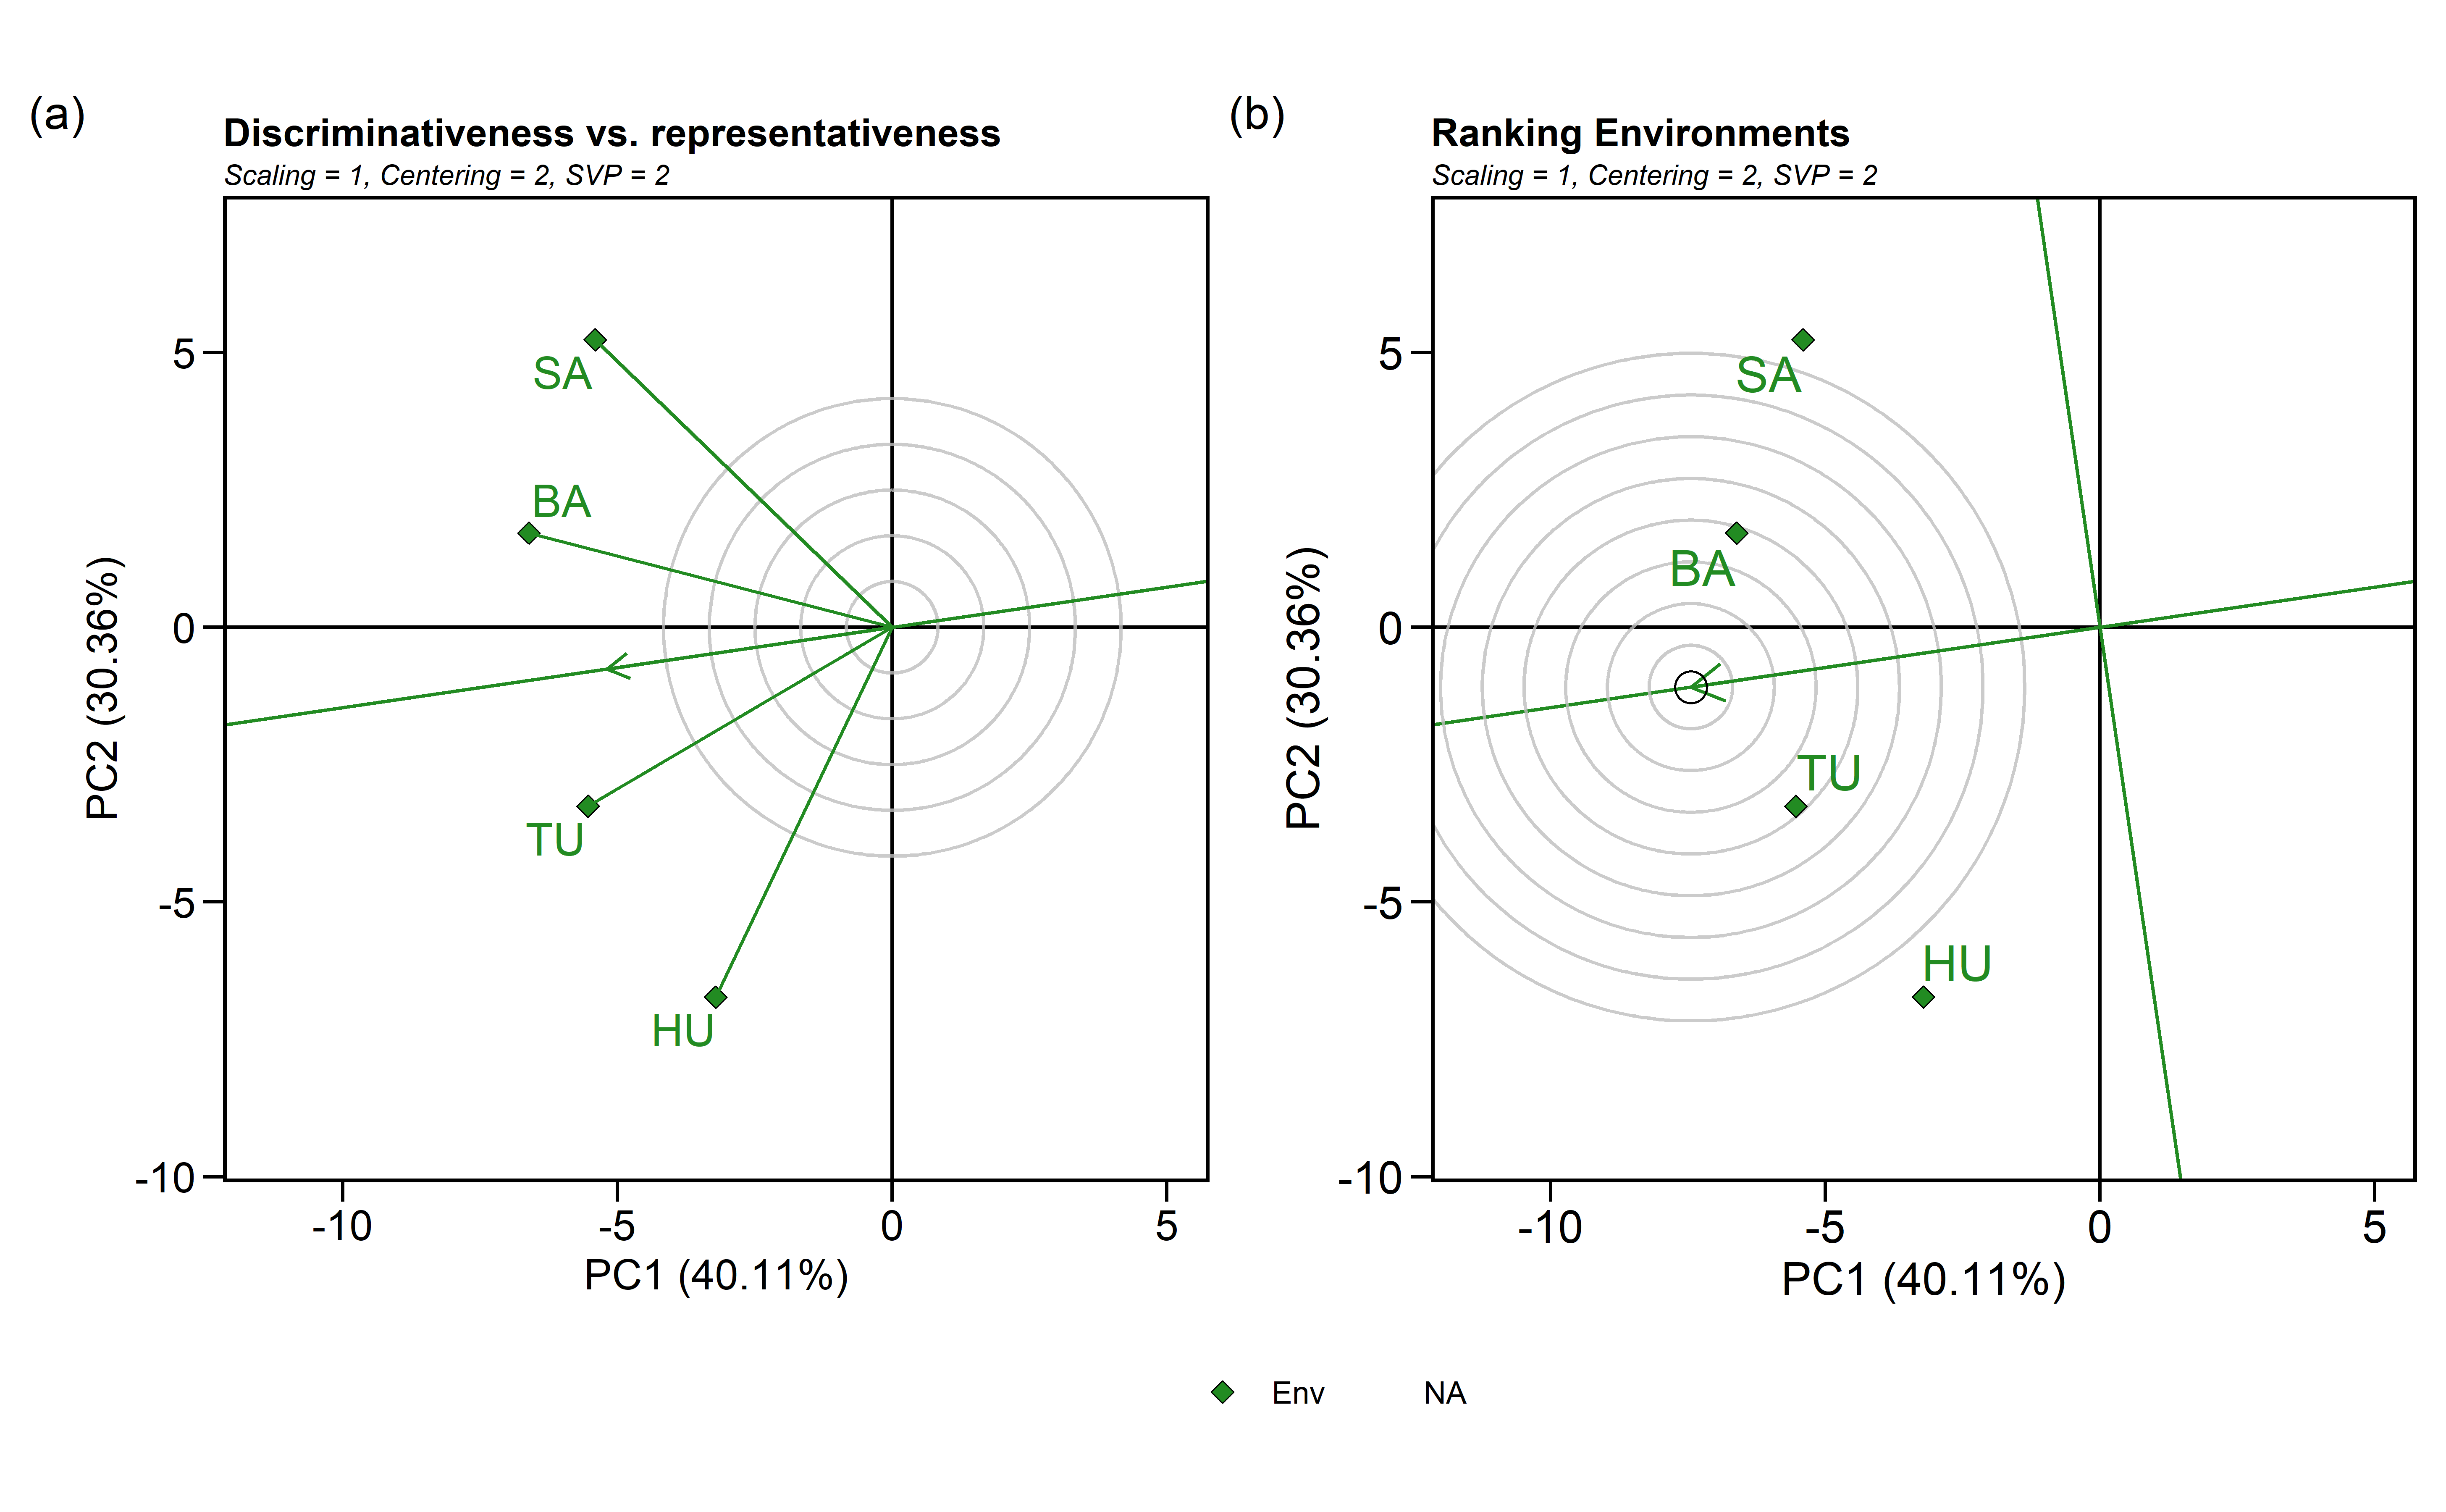
\includegraphics{figures/bb gge fig1-1} \end{center}

\hypertarget{biplot-type-3-which-won-where-1}{%
\paragraph{Biplot type 3:
Which-won-where}\label{biplot-type-3-which-won-where-1}}

GGE biplot done using:

\begin{itemize}
\tightlist
\item
  \textbf{sd}: each value is divided by the standard deviation of its
  corresponding environment.
\item
  \textbf{environment}: environment-centered (G+GE)
\item
  \textbf{genotype}: singular value is entirely partitioned into the
  environment eigenvectors, also called column metric preserving
\end{itemize}

\begin{Shaded}
\begin{Highlighting}[]
\NormalTok{gge\_model.bb }\OtherTok{\textless{}{-}} \FunctionTok{gge}\NormalTok{(blues\_stage.I\_BB, loc, name, yield,}
                     \AttributeTok{centering =} \StringTok{"environment"}\NormalTok{, }\CommentTok{\#2}
                    \AttributeTok{scaling =} \StringTok{"sd"}\NormalTok{, }\CommentTok{\#1}
                    \AttributeTok{svp =} \StringTok{"genotype"}\NormalTok{)}\CommentTok{\#2)}

\NormalTok{e }\OtherTok{\textless{}{-}} \FunctionTok{plot}\NormalTok{(gge\_model.bb, }\AttributeTok{type =} \DecValTok{3}\NormalTok{,}
          \AttributeTok{size.text.env =} \DecValTok{5}\NormalTok{,}
          \AttributeTok{plot\_theme =} \FunctionTok{theme\_metan}\NormalTok{(}\AttributeTok{grid =}  \StringTok{"both"}\NormalTok{,}\AttributeTok{color.background =} \FunctionTok{transparent\_color}\NormalTok{()),}
         \AttributeTok{axis\_expand =} \FloatTok{1.2}\NormalTok{,}
         \AttributeTok{size.line =} \FloatTok{0.7}\NormalTok{,}
         \AttributeTok{size.text.gen =} \DecValTok{4}\NormalTok{,}
         \AttributeTok{size.text.win =} \FloatTok{4.5}
         \CommentTok{\#title = F}
\NormalTok{        )}

\FunctionTok{print}\NormalTok{(e)}
\end{Highlighting}
\end{Shaded}

\begin{center}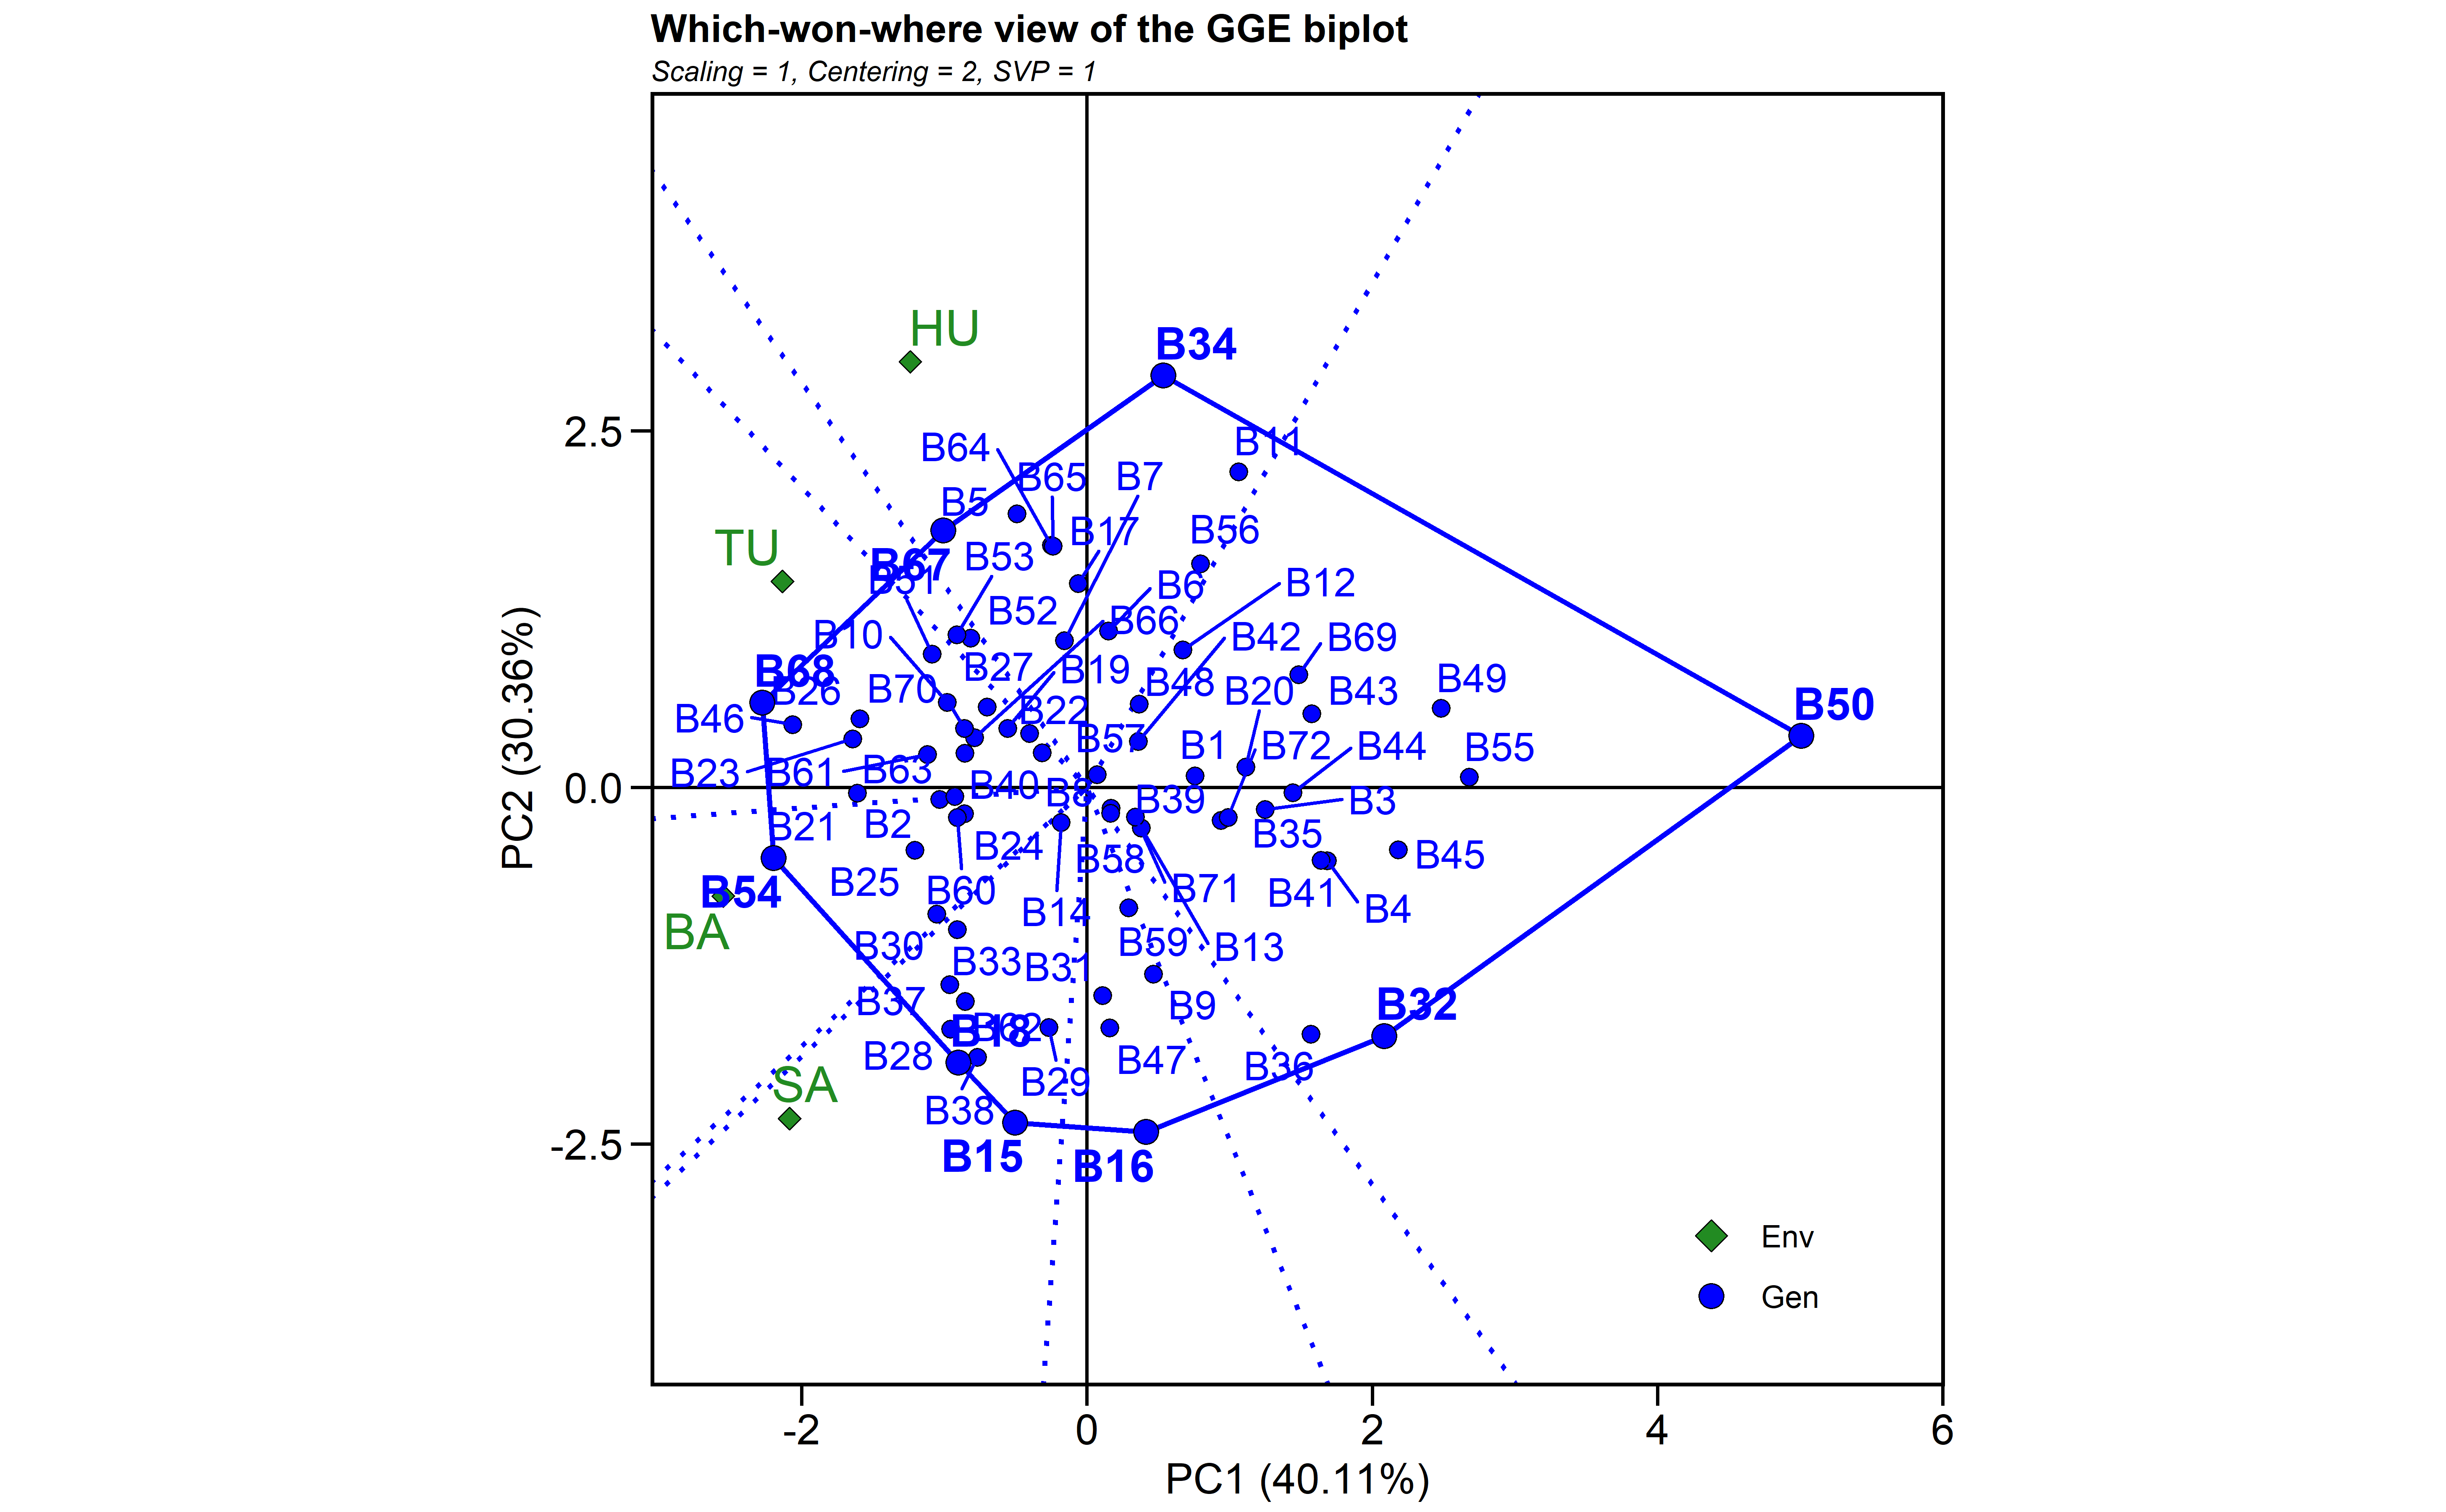
\includegraphics{figures/bb gge fig2-1} \end{center}

\hypertarget{mean-performance-and-stability-analysis-1}{%
\subsubsection{Mean performance and stability
analysis}\label{mean-performance-and-stability-analysis-1}}

WAASP index and BLUPs to estimate stability analysis.

\begin{Shaded}
\begin{Highlighting}[]
\CommentTok{\#blues\_stage.I\_BB\textless{}{-} na.omit(blues\_stage.I\_BB)}

\NormalTok{waasb\_model\_bb }\OtherTok{\textless{}{-}} 
  \FunctionTok{waasb}\NormalTok{(blues\_stage.I\_BB,}
        \AttributeTok{env =}\NormalTok{ loc,}
        \AttributeTok{gen =}\NormalTok{ name,}
        \AttributeTok{rep =}\NormalTok{ rep,}
        \AttributeTok{resp =}\NormalTok{ yield,}
        \AttributeTok{random =} \StringTok{"gen"}\NormalTok{, }\CommentTok{\#Default}
        \AttributeTok{verbose =} \ConstantTok{TRUE}\NormalTok{,}
        \AttributeTok{wresp =} \DecValTok{60}\NormalTok{) }\CommentTok{\#weight for response variable 60 and 40 for yielding and stability, respectively)}
\end{Highlighting}
\end{Shaded}

\begin{verbatim}
#> Evaluating trait yield |=================================================================================================================================================================================================| 100% 00:00:04 
#> ---------------------------------------------------------------------------
#> P-values for Likelihood Ratio Test of the analyzed traits
#> ---------------------------------------------------------------------------
#>     model    yield
#>  COMPLETE       NA
#>       GEN 5.40e-04
#>   GEN:ENV 5.48e-49
#> ---------------------------------------------------------------------------
#> All variables with significant (p < 0.05) genotype-vs-environment interaction
\end{verbatim}

\begin{Shaded}
\begin{Highlighting}[]
\NormalTok{waasb\_model}\OtherTok{\textless{}{-}}\NormalTok{ waasb\_model\_bb}\SpecialCharTok{$}\NormalTok{yield}\SpecialCharTok{$}\NormalTok{model}

\CommentTok{\#waasb\_ind \textless{}{-} gmd(waasb\_model\_bb, "WAASB")}
\CommentTok{\#print\_tbl(waasb\_ind)}

\CommentTok{\#desc \textless{}{-} c("Selected cultivar providing greater performance and stability for GY")}

\NormalTok{waasp\_plot }\OtherTok{\textless{}{-}} \FunctionTok{plot\_scores}\NormalTok{(waasb\_model\_bb, }\AttributeTok{type =} \DecValTok{3}\NormalTok{,}
          \AttributeTok{title =} \ConstantTok{FALSE}\NormalTok{,}
          \AttributeTok{size.tex.gen =} \DecValTok{4}\NormalTok{,}
          \AttributeTok{size.tex.env =} \DecValTok{4}\NormalTok{,}
          \AttributeTok{size.tex.lab =} \DecValTok{13}\NormalTok{,}
        \CommentTok{\# highlight = c("B55", "B1" , "B29", "B20" ,"B28"),}
         \AttributeTok{plot\_theme =} \FunctionTok{theme\_metan}\NormalTok{(}\AttributeTok{grid =}  \StringTok{"both"}\NormalTok{,}\AttributeTok{color.background =} \FunctionTok{transparent\_color}\NormalTok{())}
\NormalTok{        ) }\SpecialCharTok{+}
  
  \FunctionTok{geom\_mark\_rect}\NormalTok{(}\FunctionTok{aes}\NormalTok{(}\AttributeTok{filter =}\NormalTok{  Code  }\SpecialCharTok{\%in\%} \FunctionTok{c}\NormalTok{(}\StringTok{"B17"}\NormalTok{, }\StringTok{"B46"}\NormalTok{, }\StringTok{"B10"}\NormalTok{, }\StringTok{"B14"}\NormalTok{),}
\NormalTok{                     ),}
               \AttributeTok{label.fontsize =} \DecValTok{10}\NormalTok{,}
               \AttributeTok{show.legend =}\NormalTok{ F,}
               \AttributeTok{con.cap =} \DecValTok{0}\NormalTok{,}
               \AttributeTok{con.colour =} \StringTok{"red"}\NormalTok{,}
               \AttributeTok{color =} \StringTok{"red"}\NormalTok{,}
               \AttributeTok{expand =} \FloatTok{0.015}\NormalTok{,}
               \AttributeTok{label.buffer =} \FunctionTok{unit}\NormalTok{(}\DecValTok{10}\NormalTok{, }\StringTok{"cm"}\NormalTok{))}\SpecialCharTok{+}
\CommentTok{\#theme\_gray()+}
\FunctionTok{theme}\NormalTok{(}\AttributeTok{legend.position =} \FunctionTok{c}\NormalTok{(}\FloatTok{0.1}\NormalTok{, }\FloatTok{0.9}\NormalTok{),}
      \AttributeTok{legend.background =} \FunctionTok{element\_blank}\NormalTok{(),}
      \AttributeTok{legend.title =} \FunctionTok{element\_blank}\NormalTok{(),}
      \AttributeTok{aspect.ratio =} \DecValTok{1}\NormalTok{) }\SpecialCharTok{+}
  \FunctionTok{labs}\NormalTok{(}\AttributeTok{x =} \StringTok{"GY"}\NormalTok{) }

\FunctionTok{print}\NormalTok{(waasp\_plot)}
\end{Highlighting}
\end{Shaded}

\begin{center}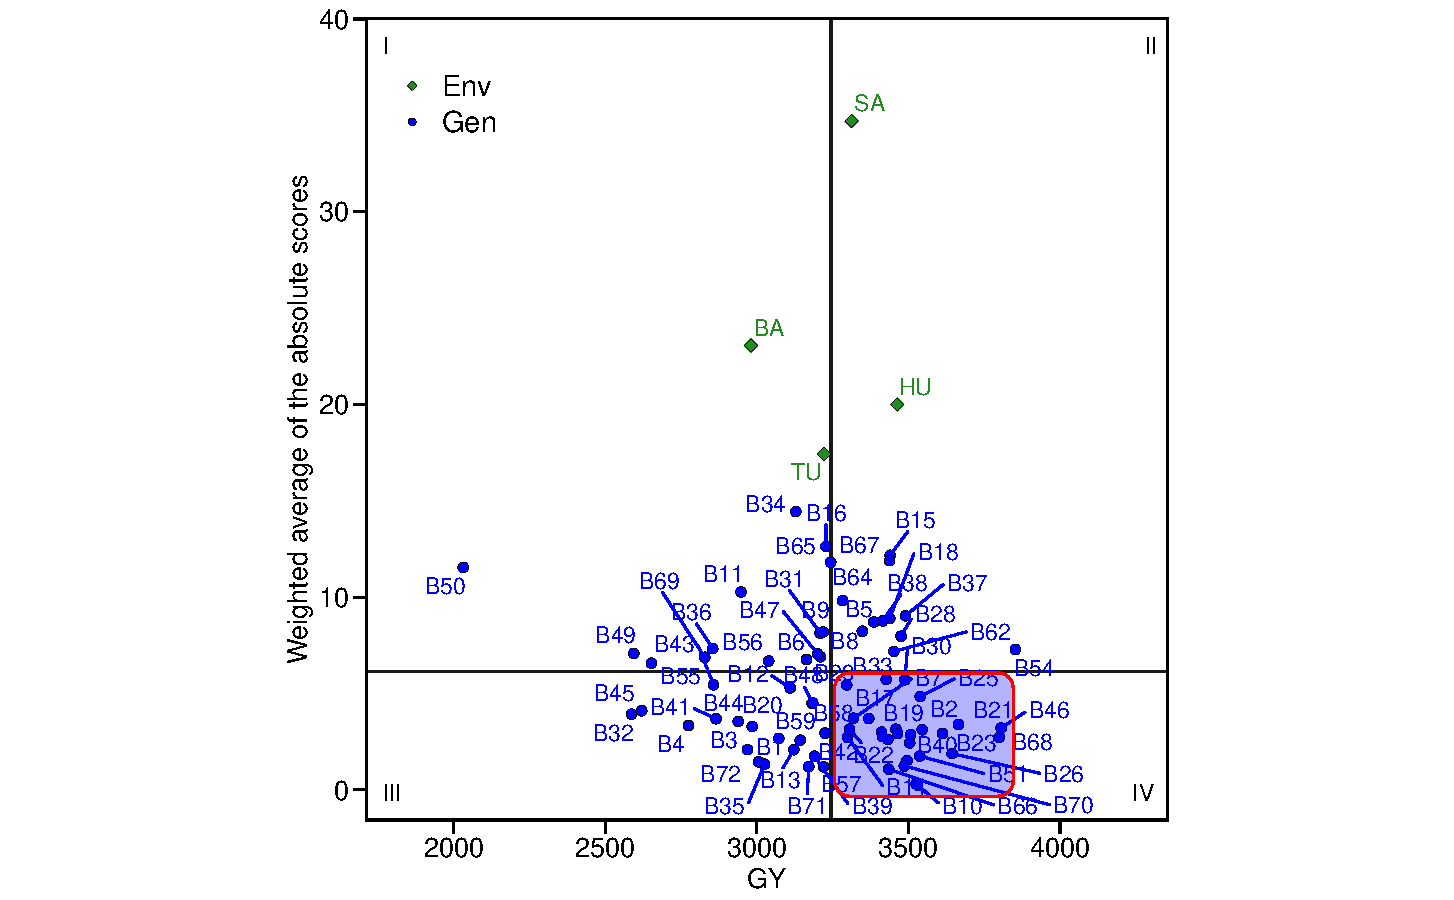
\includegraphics{figures/mod metan bb stab-1} \end{center}

\begin{Shaded}
\begin{Highlighting}[]
\NormalTok{waasb\_model\_meanWaasb}\OtherTok{\textless{}{-}}\FunctionTok{mean}\NormalTok{(waasb\_model}\SpecialCharTok{$}\NormalTok{WAASB)}
\NormalTok{waasb\_model\_meanY}\OtherTok{\textless{}{-}}\FunctionTok{mean}\NormalTok{(waasb\_model}\SpecialCharTok{$}\NormalTok{Y)}

\NormalTok{selected }\OtherTok{\textless{}{-}}\NormalTok{ waasb\_model }\SpecialCharTok{\%\textgreater{}\%}
\NormalTok{  dplyr}\SpecialCharTok{::}\FunctionTok{filter}\NormalTok{(Y }\SpecialCharTok{\textgreater{}=}\NormalTok{ waasb\_model\_meanY }\SpecialCharTok{\&}\NormalTok{ WAASB }\SpecialCharTok{\textless{}=}\NormalTok{ waasb\_model\_meanWaasb) }

\NormalTok{selected\_table }\OtherTok{\textless{}{-}}\NormalTok{ selected}

\ControlFlowTok{if}\NormalTok{ (knitr}\SpecialCharTok{::}\FunctionTok{is\_html\_output}\NormalTok{()) \{}

  \FunctionTok{print\_table}\NormalTok{(selected\_table)}
  
\NormalTok{\}}\ControlFlowTok{else}\NormalTok{\{}
  
\NormalTok{ selected\_table[,}\DecValTok{1}\SpecialCharTok{:}\DecValTok{8}\NormalTok{] }
\NormalTok{\}}
\end{Highlighting}
\end{Shaded}

\global\setlength{\Oldarrayrulewidth}{\arrayrulewidth}

\global\setlength{\Oldtabcolsep}{\tabcolsep}

\setlength{\tabcolsep}{0pt}

\renewcommand*{\arraystretch}{1.5}



\providecommand{\ascline}[3]{\noalign{\global\arrayrulewidth #1}\arrayrulecolor[HTML]{#2}\cline{#3}}

\begin{longtable}[c]{|p{0.77in}|p{0.77in}|p{0.75in}|p{0.75in}|p{0.75in}|p{0.75in}|p{0.75in}|p{0.75in}}



\ascline{1.5pt}{666666}{1-8}

\multicolumn{1}{>{\raggedright}m{\dimexpr 0.77in+0\tabcolsep}}{\textcolor[HTML]{000000}{\fontsize{9}{9}\selectfont{\global\setmainfont{Arial}{\textbf{type}}}}} & \multicolumn{1}{>{\raggedright}m{\dimexpr 0.77in+0\tabcolsep}}{\textcolor[HTML]{000000}{\fontsize{9}{9}\selectfont{\global\setmainfont{Arial}{\textbf{Code}}}}} & \multicolumn{1}{>{\raggedleft}m{\dimexpr 0.75in+0\tabcolsep}}{\textcolor[HTML]{000000}{\fontsize{9}{9}\selectfont{\global\setmainfont{Arial}{\textbf{Y}}}}} & \multicolumn{1}{>{\raggedleft}m{\dimexpr 0.75in+0\tabcolsep}}{\textcolor[HTML]{000000}{\fontsize{9}{9}\selectfont{\global\setmainfont{Arial}{\textbf{PC1}}}}} & \multicolumn{1}{>{\raggedleft}m{\dimexpr 0.75in+0\tabcolsep}}{\textcolor[HTML]{000000}{\fontsize{9}{9}\selectfont{\global\setmainfont{Arial}{\textbf{PC2}}}}} & \multicolumn{1}{>{\raggedleft}m{\dimexpr 0.75in+0\tabcolsep}}{\textcolor[HTML]{000000}{\fontsize{9}{9}\selectfont{\global\setmainfont{Arial}{\textbf{PC3}}}}} & \multicolumn{1}{>{\raggedleft}m{\dimexpr 0.75in+0\tabcolsep}}{\textcolor[HTML]{000000}{\fontsize{9}{9}\selectfont{\global\setmainfont{Arial}{\textbf{WAASB}}}}} & \multicolumn{1}{>{\raggedleft}m{\dimexpr 0.75in+0\tabcolsep}}{\textcolor[HTML]{000000}{\fontsize{9}{9}\selectfont{\global\setmainfont{Arial}{\textbf{PctResp}}}}} \\

\ascline{0.75pt}{666666}{1-8}



\multicolumn{1}{>{\raggedright}m{\dimexpr 0.77in+0\tabcolsep}}{\textcolor[HTML]{999999}{\fontsize{9}{9}\selectfont{\global\setmainfont{Arial}{\textbf{character}}}}} & \multicolumn{1}{>{\raggedright}m{\dimexpr 0.77in+0\tabcolsep}}{\textcolor[HTML]{999999}{\fontsize{9}{9}\selectfont{\global\setmainfont{Arial}{\textbf{character}}}}} & \multicolumn{1}{>{\raggedleft}m{\dimexpr 0.75in+0\tabcolsep}}{\textcolor[HTML]{999999}{\fontsize{9}{9}\selectfont{\global\setmainfont{Arial}{\textbf{numeric}}}}} & \multicolumn{1}{>{\raggedleft}m{\dimexpr 0.75in+0\tabcolsep}}{\textcolor[HTML]{999999}{\fontsize{9}{9}\selectfont{\global\setmainfont{Arial}{\textbf{numeric}}}}} & \multicolumn{1}{>{\raggedleft}m{\dimexpr 0.75in+0\tabcolsep}}{\textcolor[HTML]{999999}{\fontsize{9}{9}\selectfont{\global\setmainfont{Arial}{\textbf{numeric}}}}} & \multicolumn{1}{>{\raggedleft}m{\dimexpr 0.75in+0\tabcolsep}}{\textcolor[HTML]{999999}{\fontsize{9}{9}\selectfont{\global\setmainfont{Arial}{\textbf{numeric}}}}} & \multicolumn{1}{>{\raggedleft}m{\dimexpr 0.75in+0\tabcolsep}}{\textcolor[HTML]{999999}{\fontsize{9}{9}\selectfont{\global\setmainfont{Arial}{\textbf{numeric}}}}} & \multicolumn{1}{>{\raggedleft}m{\dimexpr 0.75in+0\tabcolsep}}{\textcolor[HTML]{999999}{\fontsize{9}{9}\selectfont{\global\setmainfont{Arial}{\textbf{numeric}}}}} \\

\ascline{1.5pt}{666666}{1-8}\endfirsthead

\ascline{1.5pt}{666666}{1-8}

\multicolumn{1}{>{\raggedright}m{\dimexpr 0.77in+0\tabcolsep}}{\textcolor[HTML]{000000}{\fontsize{9}{9}\selectfont{\global\setmainfont{Arial}{\textbf{type}}}}} & \multicolumn{1}{>{\raggedright}m{\dimexpr 0.77in+0\tabcolsep}}{\textcolor[HTML]{000000}{\fontsize{9}{9}\selectfont{\global\setmainfont{Arial}{\textbf{Code}}}}} & \multicolumn{1}{>{\raggedleft}m{\dimexpr 0.75in+0\tabcolsep}}{\textcolor[HTML]{000000}{\fontsize{9}{9}\selectfont{\global\setmainfont{Arial}{\textbf{Y}}}}} & \multicolumn{1}{>{\raggedleft}m{\dimexpr 0.75in+0\tabcolsep}}{\textcolor[HTML]{000000}{\fontsize{9}{9}\selectfont{\global\setmainfont{Arial}{\textbf{PC1}}}}} & \multicolumn{1}{>{\raggedleft}m{\dimexpr 0.75in+0\tabcolsep}}{\textcolor[HTML]{000000}{\fontsize{9}{9}\selectfont{\global\setmainfont{Arial}{\textbf{PC2}}}}} & \multicolumn{1}{>{\raggedleft}m{\dimexpr 0.75in+0\tabcolsep}}{\textcolor[HTML]{000000}{\fontsize{9}{9}\selectfont{\global\setmainfont{Arial}{\textbf{PC3}}}}} & \multicolumn{1}{>{\raggedleft}m{\dimexpr 0.75in+0\tabcolsep}}{\textcolor[HTML]{000000}{\fontsize{9}{9}\selectfont{\global\setmainfont{Arial}{\textbf{WAASB}}}}} & \multicolumn{1}{>{\raggedleft}m{\dimexpr 0.75in+0\tabcolsep}}{\textcolor[HTML]{000000}{\fontsize{9}{9}\selectfont{\global\setmainfont{Arial}{\textbf{PctResp}}}}} \\

\ascline{0.75pt}{666666}{1-8}



\multicolumn{1}{>{\raggedright}m{\dimexpr 0.77in+0\tabcolsep}}{\textcolor[HTML]{999999}{\fontsize{9}{9}\selectfont{\global\setmainfont{Arial}{\textbf{character}}}}} & \multicolumn{1}{>{\raggedright}m{\dimexpr 0.77in+0\tabcolsep}}{\textcolor[HTML]{999999}{\fontsize{9}{9}\selectfont{\global\setmainfont{Arial}{\textbf{character}}}}} & \multicolumn{1}{>{\raggedleft}m{\dimexpr 0.75in+0\tabcolsep}}{\textcolor[HTML]{999999}{\fontsize{9}{9}\selectfont{\global\setmainfont{Arial}{\textbf{numeric}}}}} & \multicolumn{1}{>{\raggedleft}m{\dimexpr 0.75in+0\tabcolsep}}{\textcolor[HTML]{999999}{\fontsize{9}{9}\selectfont{\global\setmainfont{Arial}{\textbf{numeric}}}}} & \multicolumn{1}{>{\raggedleft}m{\dimexpr 0.75in+0\tabcolsep}}{\textcolor[HTML]{999999}{\fontsize{9}{9}\selectfont{\global\setmainfont{Arial}{\textbf{numeric}}}}} & \multicolumn{1}{>{\raggedleft}m{\dimexpr 0.75in+0\tabcolsep}}{\textcolor[HTML]{999999}{\fontsize{9}{9}\selectfont{\global\setmainfont{Arial}{\textbf{numeric}}}}} & \multicolumn{1}{>{\raggedleft}m{\dimexpr 0.75in+0\tabcolsep}}{\textcolor[HTML]{999999}{\fontsize{9}{9}\selectfont{\global\setmainfont{Arial}{\textbf{numeric}}}}} & \multicolumn{1}{>{\raggedleft}m{\dimexpr 0.75in+0\tabcolsep}}{\textcolor[HTML]{999999}{\fontsize{9}{9}\selectfont{\global\setmainfont{Arial}{\textbf{numeric}}}}} \\

\ascline{1.5pt}{666666}{1-8}\endhead



\multicolumn{8}{>{\raggedright}m{\dimexpr 6.05in+14\tabcolsep}}{\textcolor[HTML]{000000}{\fontsize{9}{9}\selectfont{\global\setmainfont{Arial}{n:\ 26}}}} \\

\ascline{0.75pt}{666666}{1-8}\endfoot



\multicolumn{1}{>{\raggedright}m{\dimexpr 0.77in+0\tabcolsep}}{\textcolor[HTML]{000000}{\fontsize{9}{9}\selectfont{\global\setmainfont{Arial}{GEN}}}} & \multicolumn{1}{>{\raggedright}m{\dimexpr 0.77in+0\tabcolsep}}{\textcolor[HTML]{000000}{\fontsize{9}{9}\selectfont{\global\setmainfont{Arial}{B10}}}} & \multicolumn{1}{>{\raggedleft}m{\dimexpr 0.75in+0\tabcolsep}}{\textcolor[HTML]{000000}{\fontsize{9}{9}\selectfont{\global\setmainfont{Arial}{3,525.7}}}} & \multicolumn{1}{>{\raggedleft}m{\dimexpr 0.75in+0\tabcolsep}}{\textcolor[HTML]{000000}{\fontsize{9}{9}\selectfont{\global\setmainfont{Arial}{0.1}}}} & \multicolumn{1}{>{\raggedleft}m{\dimexpr 0.75in+0\tabcolsep}}{\textcolor[HTML]{000000}{\fontsize{9}{9}\selectfont{\global\setmainfont{Arial}{-0.1}}}} & \multicolumn{1}{>{\raggedleft}m{\dimexpr 0.75in+0\tabcolsep}}{\textcolor[HTML]{000000}{\fontsize{9}{9}\selectfont{\global\setmainfont{Arial}{1.4}}}} & \multicolumn{1}{>{\raggedleft}m{\dimexpr 0.75in+0\tabcolsep}}{\textcolor[HTML]{000000}{\fontsize{9}{9}\selectfont{\global\setmainfont{Arial}{0.3}}}} & \multicolumn{1}{>{\raggedleft}m{\dimexpr 0.75in+0\tabcolsep}}{\textcolor[HTML]{000000}{\fontsize{9}{9}\selectfont{\global\setmainfont{Arial}{82.0}}}} \\

\ascline{0.75pt}{666666}{1-8}



\multicolumn{1}{>{\raggedright}m{\dimexpr 0.77in+0\tabcolsep}}{\textcolor[HTML]{000000}{\fontsize{9}{9}\selectfont{\global\setmainfont{Arial}{GEN}}}} & \multicolumn{1}{>{\raggedright}m{\dimexpr 0.77in+0\tabcolsep}}{\textcolor[HTML]{000000}{\fontsize{9}{9}\selectfont{\global\setmainfont{Arial}{B14}}}} & \multicolumn{1}{>{\raggedleft}m{\dimexpr 0.75in+0\tabcolsep}}{\textcolor[HTML]{000000}{\fontsize{9}{9}\selectfont{\global\setmainfont{Arial}{3,299.5}}}} & \multicolumn{1}{>{\raggedleft}m{\dimexpr 0.75in+0\tabcolsep}}{\textcolor[HTML]{000000}{\fontsize{9}{9}\selectfont{\global\setmainfont{Arial}{1.7}}}} & \multicolumn{1}{>{\raggedleft}m{\dimexpr 0.75in+0\tabcolsep}}{\textcolor[HTML]{000000}{\fontsize{9}{9}\selectfont{\global\setmainfont{Arial}{4.6}}}} & \multicolumn{1}{>{\raggedleft}m{\dimexpr 0.75in+0\tabcolsep}}{\textcolor[HTML]{000000}{\fontsize{9}{9}\selectfont{\global\setmainfont{Arial}{3.1}}}} & \multicolumn{1}{>{\raggedleft}m{\dimexpr 0.75in+0\tabcolsep}}{\textcolor[HTML]{000000}{\fontsize{9}{9}\selectfont{\global\setmainfont{Arial}{2.7}}}} & \multicolumn{1}{>{\raggedleft}m{\dimexpr 0.75in+0\tabcolsep}}{\textcolor[HTML]{000000}{\fontsize{9}{9}\selectfont{\global\setmainfont{Arial}{69.6}}}} \\

\ascline{0.75pt}{666666}{1-8}



\multicolumn{1}{>{\raggedright}m{\dimexpr 0.77in+0\tabcolsep}}{\textcolor[HTML]{000000}{\fontsize{9}{9}\selectfont{\global\setmainfont{Arial}{GEN}}}} & \multicolumn{1}{>{\raggedright}m{\dimexpr 0.77in+0\tabcolsep}}{\textcolor[HTML]{000000}{\fontsize{9}{9}\selectfont{\global\setmainfont{Arial}{B17}}}} & \multicolumn{1}{>{\raggedleft}m{\dimexpr 0.75in+0\tabcolsep}}{\textcolor[HTML]{000000}{\fontsize{9}{9}\selectfont{\global\setmainfont{Arial}{3,296.5}}}} & \multicolumn{1}{>{\raggedleft}m{\dimexpr 0.75in+0\tabcolsep}}{\textcolor[HTML]{000000}{\fontsize{9}{9}\selectfont{\global\setmainfont{Arial}{-6.9}}}} & \multicolumn{1}{>{\raggedleft}m{\dimexpr 0.75in+0\tabcolsep}}{\textcolor[HTML]{000000}{\fontsize{9}{9}\selectfont{\global\setmainfont{Arial}{-4.8}}}} & \multicolumn{1}{>{\raggedleft}m{\dimexpr 0.75in+0\tabcolsep}}{\textcolor[HTML]{000000}{\fontsize{9}{9}\selectfont{\global\setmainfont{Arial}{1.4}}}} & \multicolumn{1}{>{\raggedleft}m{\dimexpr 0.75in+0\tabcolsep}}{\textcolor[HTML]{000000}{\fontsize{9}{9}\selectfont{\global\setmainfont{Arial}{5.4}}}} & \multicolumn{1}{>{\raggedleft}m{\dimexpr 0.75in+0\tabcolsep}}{\textcolor[HTML]{000000}{\fontsize{9}{9}\selectfont{\global\setmainfont{Arial}{69.4}}}} \\

\ascline{0.75pt}{666666}{1-8}



\multicolumn{1}{>{\raggedright}m{\dimexpr 0.77in+0\tabcolsep}}{\textcolor[HTML]{000000}{\fontsize{9}{9}\selectfont{\global\setmainfont{Arial}{GEN}}}} & \multicolumn{1}{>{\raggedright}m{\dimexpr 0.77in+0\tabcolsep}}{\textcolor[HTML]{000000}{\fontsize{9}{9}\selectfont{\global\setmainfont{Arial}{B19}}}} & \multicolumn{1}{>{\raggedleft}m{\dimexpr 0.75in+0\tabcolsep}}{\textcolor[HTML]{000000}{\fontsize{9}{9}\selectfont{\global\setmainfont{Arial}{3,369.1}}}} & \multicolumn{1}{>{\raggedleft}m{\dimexpr 0.75in+0\tabcolsep}}{\textcolor[HTML]{000000}{\fontsize{9}{9}\selectfont{\global\setmainfont{Arial}{-0.5}}}} & \multicolumn{1}{>{\raggedleft}m{\dimexpr 0.75in+0\tabcolsep}}{\textcolor[HTML]{000000}{\fontsize{9}{9}\selectfont{\global\setmainfont{Arial}{-8.0}}}} & \multicolumn{1}{>{\raggedleft}m{\dimexpr 0.75in+0\tabcolsep}}{\textcolor[HTML]{000000}{\fontsize{9}{9}\selectfont{\global\setmainfont{Arial}{-7.6}}}} & \multicolumn{1}{>{\raggedleft}m{\dimexpr 0.75in+0\tabcolsep}}{\textcolor[HTML]{000000}{\fontsize{9}{9}\selectfont{\global\setmainfont{Arial}{3.7}}}} & \multicolumn{1}{>{\raggedleft}m{\dimexpr 0.75in+0\tabcolsep}}{\textcolor[HTML]{000000}{\fontsize{9}{9}\selectfont{\global\setmainfont{Arial}{73.4}}}} \\

\ascline{0.75pt}{666666}{1-8}



\multicolumn{1}{>{\raggedright}m{\dimexpr 0.77in+0\tabcolsep}}{\textcolor[HTML]{000000}{\fontsize{9}{9}\selectfont{\global\setmainfont{Arial}{GEN}}}} & \multicolumn{1}{>{\raggedright}m{\dimexpr 0.77in+0\tabcolsep}}{\textcolor[HTML]{000000}{\fontsize{9}{9}\selectfont{\global\setmainfont{Arial}{B2}}}} & \multicolumn{1}{>{\raggedleft}m{\dimexpr 0.75in+0\tabcolsep}}{\textcolor[HTML]{000000}{\fontsize{9}{9}\selectfont{\global\setmainfont{Arial}{3,545.5}}}} & \multicolumn{1}{>{\raggedleft}m{\dimexpr 0.75in+0\tabcolsep}}{\textcolor[HTML]{000000}{\fontsize{9}{9}\selectfont{\global\setmainfont{Arial}{4.6}}}} & \multicolumn{1}{>{\raggedleft}m{\dimexpr 0.75in+0\tabcolsep}}{\textcolor[HTML]{000000}{\fontsize{9}{9}\selectfont{\global\setmainfont{Arial}{0.2}}}} & \multicolumn{1}{>{\raggedleft}m{\dimexpr 0.75in+0\tabcolsep}}{\textcolor[HTML]{000000}{\fontsize{9}{9}\selectfont{\global\setmainfont{Arial}{2.6}}}} & \multicolumn{1}{>{\raggedleft}m{\dimexpr 0.75in+0\tabcolsep}}{\textcolor[HTML]{000000}{\fontsize{9}{9}\selectfont{\global\setmainfont{Arial}{3.1}}}} & \multicolumn{1}{>{\raggedleft}m{\dimexpr 0.75in+0\tabcolsep}}{\textcolor[HTML]{000000}{\fontsize{9}{9}\selectfont{\global\setmainfont{Arial}{83.1}}}} \\

\ascline{0.75pt}{666666}{1-8}



\multicolumn{1}{>{\raggedright}m{\dimexpr 0.77in+0\tabcolsep}}{\textcolor[HTML]{000000}{\fontsize{9}{9}\selectfont{\global\setmainfont{Arial}{GEN}}}} & \multicolumn{1}{>{\raggedright}m{\dimexpr 0.77in+0\tabcolsep}}{\textcolor[HTML]{000000}{\fontsize{9}{9}\selectfont{\global\setmainfont{Arial}{B21}}}} & \multicolumn{1}{>{\raggedleft}m{\dimexpr 0.75in+0\tabcolsep}}{\textcolor[HTML]{000000}{\fontsize{9}{9}\selectfont{\global\setmainfont{Arial}{3,665.5}}}} & \multicolumn{1}{>{\raggedleft}m{\dimexpr 0.75in+0\tabcolsep}}{\textcolor[HTML]{000000}{\fontsize{9}{9}\selectfont{\global\setmainfont{Arial}{5.0}}}} & \multicolumn{1}{>{\raggedleft}m{\dimexpr 0.75in+0\tabcolsep}}{\textcolor[HTML]{000000}{\fontsize{9}{9}\selectfont{\global\setmainfont{Arial}{0.9}}}} & \multicolumn{1}{>{\raggedleft}m{\dimexpr 0.75in+0\tabcolsep}}{\textcolor[HTML]{000000}{\fontsize{9}{9}\selectfont{\global\setmainfont{Arial}{-1.8}}}} & \multicolumn{1}{>{\raggedleft}m{\dimexpr 0.75in+0\tabcolsep}}{\textcolor[HTML]{000000}{\fontsize{9}{9}\selectfont{\global\setmainfont{Arial}{3.4}}}} & \multicolumn{1}{>{\raggedleft}m{\dimexpr 0.75in+0\tabcolsep}}{\textcolor[HTML]{000000}{\fontsize{9}{9}\selectfont{\global\setmainfont{Arial}{89.7}}}} \\

\ascline{0.75pt}{666666}{1-8}



\multicolumn{1}{>{\raggedright}m{\dimexpr 0.77in+0\tabcolsep}}{\textcolor[HTML]{000000}{\fontsize{9}{9}\selectfont{\global\setmainfont{Arial}{GEN}}}} & \multicolumn{1}{>{\raggedright}m{\dimexpr 0.77in+0\tabcolsep}}{\textcolor[HTML]{000000}{\fontsize{9}{9}\selectfont{\global\setmainfont{Arial}{B22}}}} & \multicolumn{1}{>{\raggedleft}m{\dimexpr 0.75in+0\tabcolsep}}{\textcolor[HTML]{000000}{\fontsize{9}{9}\selectfont{\global\setmainfont{Arial}{3,305.2}}}} & \multicolumn{1}{>{\raggedleft}m{\dimexpr 0.75in+0\tabcolsep}}{\textcolor[HTML]{000000}{\fontsize{9}{9}\selectfont{\global\setmainfont{Arial}{-2.3}}}} & \multicolumn{1}{>{\raggedleft}m{\dimexpr 0.75in+0\tabcolsep}}{\textcolor[HTML]{000000}{\fontsize{9}{9}\selectfont{\global\setmainfont{Arial}{-2.2}}}} & \multicolumn{1}{>{\raggedleft}m{\dimexpr 0.75in+0\tabcolsep}}{\textcolor[HTML]{000000}{\fontsize{9}{9}\selectfont{\global\setmainfont{Arial}{-7.5}}}} & \multicolumn{1}{>{\raggedleft}m{\dimexpr 0.75in+0\tabcolsep}}{\textcolor[HTML]{000000}{\fontsize{9}{9}\selectfont{\global\setmainfont{Arial}{3.2}}}} & \multicolumn{1}{>{\raggedleft}m{\dimexpr 0.75in+0\tabcolsep}}{\textcolor[HTML]{000000}{\fontsize{9}{9}\selectfont{\global\setmainfont{Arial}{69.9}}}} \\

\ascline{0.75pt}{666666}{1-8}



\multicolumn{1}{>{\raggedright}m{\dimexpr 0.77in+0\tabcolsep}}{\textcolor[HTML]{000000}{\fontsize{9}{9}\selectfont{\global\setmainfont{Arial}{GEN}}}} & \multicolumn{1}{>{\raggedright}m{\dimexpr 0.77in+0\tabcolsep}}{\textcolor[HTML]{000000}{\fontsize{9}{9}\selectfont{\global\setmainfont{Arial}{B23}}}} & \multicolumn{1}{>{\raggedleft}m{\dimexpr 0.75in+0\tabcolsep}}{\textcolor[HTML]{000000}{\fontsize{9}{9}\selectfont{\global\setmainfont{Arial}{3,612.8}}}} & \multicolumn{1}{>{\raggedleft}m{\dimexpr 0.75in+0\tabcolsep}}{\textcolor[HTML]{000000}{\fontsize{9}{9}\selectfont{\global\setmainfont{Arial}{0.1}}}} & \multicolumn{1}{>{\raggedleft}m{\dimexpr 0.75in+0\tabcolsep}}{\textcolor[HTML]{000000}{\fontsize{9}{9}\selectfont{\global\setmainfont{Arial}{6.2}}}} & \multicolumn{1}{>{\raggedleft}m{\dimexpr 0.75in+0\tabcolsep}}{\textcolor[HTML]{000000}{\fontsize{9}{9}\selectfont{\global\setmainfont{Arial}{-7.4}}}} & \multicolumn{1}{>{\raggedleft}m{\dimexpr 0.75in+0\tabcolsep}}{\textcolor[HTML]{000000}{\fontsize{9}{9}\selectfont{\global\setmainfont{Arial}{2.9}}}} & \multicolumn{1}{>{\raggedleft}m{\dimexpr 0.75in+0\tabcolsep}}{\textcolor[HTML]{000000}{\fontsize{9}{9}\selectfont{\global\setmainfont{Arial}{86.8}}}} \\

\ascline{0.75pt}{666666}{1-8}



\multicolumn{1}{>{\raggedright}m{\dimexpr 0.77in+0\tabcolsep}}{\textcolor[HTML]{000000}{\fontsize{9}{9}\selectfont{\global\setmainfont{Arial}{GEN}}}} & \multicolumn{1}{>{\raggedright}m{\dimexpr 0.77in+0\tabcolsep}}{\textcolor[HTML]{000000}{\fontsize{9}{9}\selectfont{\global\setmainfont{Arial}{B25}}}} & \multicolumn{1}{>{\raggedleft}m{\dimexpr 0.75in+0\tabcolsep}}{\textcolor[HTML]{000000}{\fontsize{9}{9}\selectfont{\global\setmainfont{Arial}{3,539.1}}}} & \multicolumn{1}{>{\raggedleft}m{\dimexpr 0.75in+0\tabcolsep}}{\textcolor[HTML]{000000}{\fontsize{9}{9}\selectfont{\global\setmainfont{Arial}{4.7}}}} & \multicolumn{1}{>{\raggedleft}m{\dimexpr 0.75in+0\tabcolsep}}{\textcolor[HTML]{000000}{\fontsize{9}{9}\selectfont{\global\setmainfont{Arial}{8.2}}}} & \multicolumn{1}{>{\raggedleft}m{\dimexpr 0.75in+0\tabcolsep}}{\textcolor[HTML]{000000}{\fontsize{9}{9}\selectfont{\global\setmainfont{Arial}{-0.2}}}} & \multicolumn{1}{>{\raggedleft}m{\dimexpr 0.75in+0\tabcolsep}}{\textcolor[HTML]{000000}{\fontsize{9}{9}\selectfont{\global\setmainfont{Arial}{4.8}}}} & \multicolumn{1}{>{\raggedleft}m{\dimexpr 0.75in+0\tabcolsep}}{\textcolor[HTML]{000000}{\fontsize{9}{9}\selectfont{\global\setmainfont{Arial}{82.8}}}} \\

\ascline{1.5pt}{666666}{1-8}



\end{longtable}



\arrayrulecolor[HTML]{000000}

\global\setlength{\arrayrulewidth}{\Oldarrayrulewidth}

\global\setlength{\tabcolsep}{\Oldtabcolsep}

\renewcommand*{\arraystretch}{1}

\begin{Shaded}
\begin{Highlighting}[]
\CommentTok{\#selected$Code}
\end{Highlighting}
\end{Shaded}

\hypertarget{selection-differentials-1}{%
\paragraph{Selection differentials}\label{selection-differentials-1}}

\begin{Shaded}
\begin{Highlighting}[]
\CommentTok{\#Create a data frame with BLUPS {-} selected and non{-}selected}
\NormalTok{blups\_sel }\OtherTok{\textless{}{-}}
  \FunctionTok{gmd}\NormalTok{(waasb\_model\_bb, }\StringTok{"blupge"}\NormalTok{) }\SpecialCharTok{\%\textgreater{}\%}
  \FunctionTok{add\_cols}\NormalTok{(}\AttributeTok{SELECTED =} \FunctionTok{ifelse}\NormalTok{(GEN }\SpecialCharTok{\%in\%}\NormalTok{ selected}\SpecialCharTok{$}\NormalTok{Code, }\StringTok{"yes"}\NormalTok{, }\StringTok{"no"}\NormalTok{)) }\SpecialCharTok{\%\textgreater{}\%} 
\NormalTok{    dplyr}\SpecialCharTok{::}\FunctionTok{rename}\NormalTok{(}\AttributeTok{BLUPs\_sel =}\NormalTok{ yield) }\SpecialCharTok{\%\textgreater{}\%} 
  \FunctionTok{droplevels}\NormalTok{()}

\NormalTok{blups\_sel\_mean}\OtherTok{\textless{}{-}}
  \FunctionTok{gmd}\NormalTok{(waasb\_model\_bb, }\StringTok{"blupge"}\NormalTok{) }\SpecialCharTok{\%\textgreater{}\%}
  \FunctionTok{add\_cols}\NormalTok{(}\AttributeTok{SELECTED =} \FunctionTok{ifelse}\NormalTok{(GEN }\SpecialCharTok{\%in\%}\NormalTok{ selected}\SpecialCharTok{$}\NormalTok{Code, }\StringTok{"yes"}\NormalTok{, }\StringTok{"no"}\NormalTok{)) }\SpecialCharTok{\%\textgreater{}\%} 
  \FunctionTok{filter}\NormalTok{(SELECTED }\SpecialCharTok{==} \StringTok{"yes"}\NormalTok{) }\SpecialCharTok{\%\textgreater{}\%} 
\NormalTok{  dplyr}\SpecialCharTok{::}\FunctionTok{summarise}\NormalTok{(}\AttributeTok{mean\_GY =} \FunctionTok{mean}\NormalTok{(yield,}\AttributeTok{na.rm =} \ConstantTok{TRUE}\NormalTok{), }\AttributeTok{n =} \FunctionTok{n}\NormalTok{()) }

\CommentTok{\# Create a data frame with the waasb index {-} selected and non{-}selected}
\NormalTok{waasb\_sel }\OtherTok{\textless{}{-}}
  \FunctionTok{gmd}\NormalTok{(waasb\_model\_bb, }\StringTok{"WAASB"}\NormalTok{) }\SpecialCharTok{\%\textgreater{}\%}
  \FunctionTok{add\_cols}\NormalTok{(}\AttributeTok{SELECTED =} \FunctionTok{ifelse}\NormalTok{(GEN }\SpecialCharTok{\%in\%}\NormalTok{ selected}\SpecialCharTok{$}\NormalTok{Code, }\StringTok{"yes"}\NormalTok{, }\StringTok{"no"}\NormalTok{)) }\SpecialCharTok{\%\textgreater{}\%} 
\NormalTok{  dplyr}\SpecialCharTok{::}\FunctionTok{rename}\NormalTok{(}\AttributeTok{WAASB\_sel =}\NormalTok{ yield) }\SpecialCharTok{\%\textgreater{}\%} 
  \FunctionTok{droplevels}\NormalTok{()}
\CommentTok{\#str(waasb\_sel)}

\NormalTok{waasb\_sel\_mean}\OtherTok{\textless{}{-}}
  \FunctionTok{gmd}\NormalTok{(waasb\_model\_bb, }\StringTok{"WAASB"}\NormalTok{) }\SpecialCharTok{\%\textgreater{}\%}
  \FunctionTok{add\_cols}\NormalTok{(}\AttributeTok{SELECTED =} \FunctionTok{ifelse}\NormalTok{(GEN }\SpecialCharTok{\%in\%}\NormalTok{ selected}\SpecialCharTok{$}\NormalTok{Code, }\StringTok{"yes"}\NormalTok{, }\StringTok{"no"}\NormalTok{)) }\SpecialCharTok{\%\textgreater{}\%} 
  \FunctionTok{filter}\NormalTok{(SELECTED }\SpecialCharTok{==} \StringTok{"yes"}\NormalTok{) }\SpecialCharTok{\%\textgreater{}\%} 
\NormalTok{  dplyr}\SpecialCharTok{::}\FunctionTok{summarise}\NormalTok{(}\AttributeTok{mean\_GY =} \FunctionTok{mean}\NormalTok{(yield,}\AttributeTok{na.rm =} \ConstantTok{TRUE}\NormalTok{), }\AttributeTok{n =} \FunctionTok{n}\NormalTok{()) }

\NormalTok{p1}\OtherTok{\textless{}{-}} \FunctionTok{plot\_selected}\NormalTok{(blups\_sel, GEN, BLUPs\_sel, }\AttributeTok{mean\_sel =}\NormalTok{ blups\_sel\_mean}\SpecialCharTok{$}\NormalTok{mean\_GY) }\SpecialCharTok{+}
  \FunctionTok{labs}\NormalTok{(}\AttributeTok{y =} \StringTok{"GY"}\NormalTok{)}

\NormalTok{p3}\OtherTok{\textless{}{-}} \FunctionTok{plot\_selected}\NormalTok{(waasb\_sel, GEN, WAASB\_sel, }\AttributeTok{mean\_sel =}\NormalTok{ waasb\_sel\_mean}\SpecialCharTok{$}\NormalTok{mean\_GY) }\SpecialCharTok{+}
  \FunctionTok{labs}\NormalTok{(}\AttributeTok{y =} \StringTok{"WAASB index"}\NormalTok{)}

\FunctionTok{arrange\_ggplot}\NormalTok{(p1, p3,}
  \AttributeTok{guides =} \StringTok{"collect"}\NormalTok{,}
  \AttributeTok{tag\_levels =} \StringTok{"a"}\NormalTok{,}
  \AttributeTok{tag\_prefix =} \StringTok{"("}\NormalTok{,}
  \AttributeTok{tag\_suffix =} \StringTok{")"}\NormalTok{)}
\end{Highlighting}
\end{Shaded}

\begin{figure}

{\centering 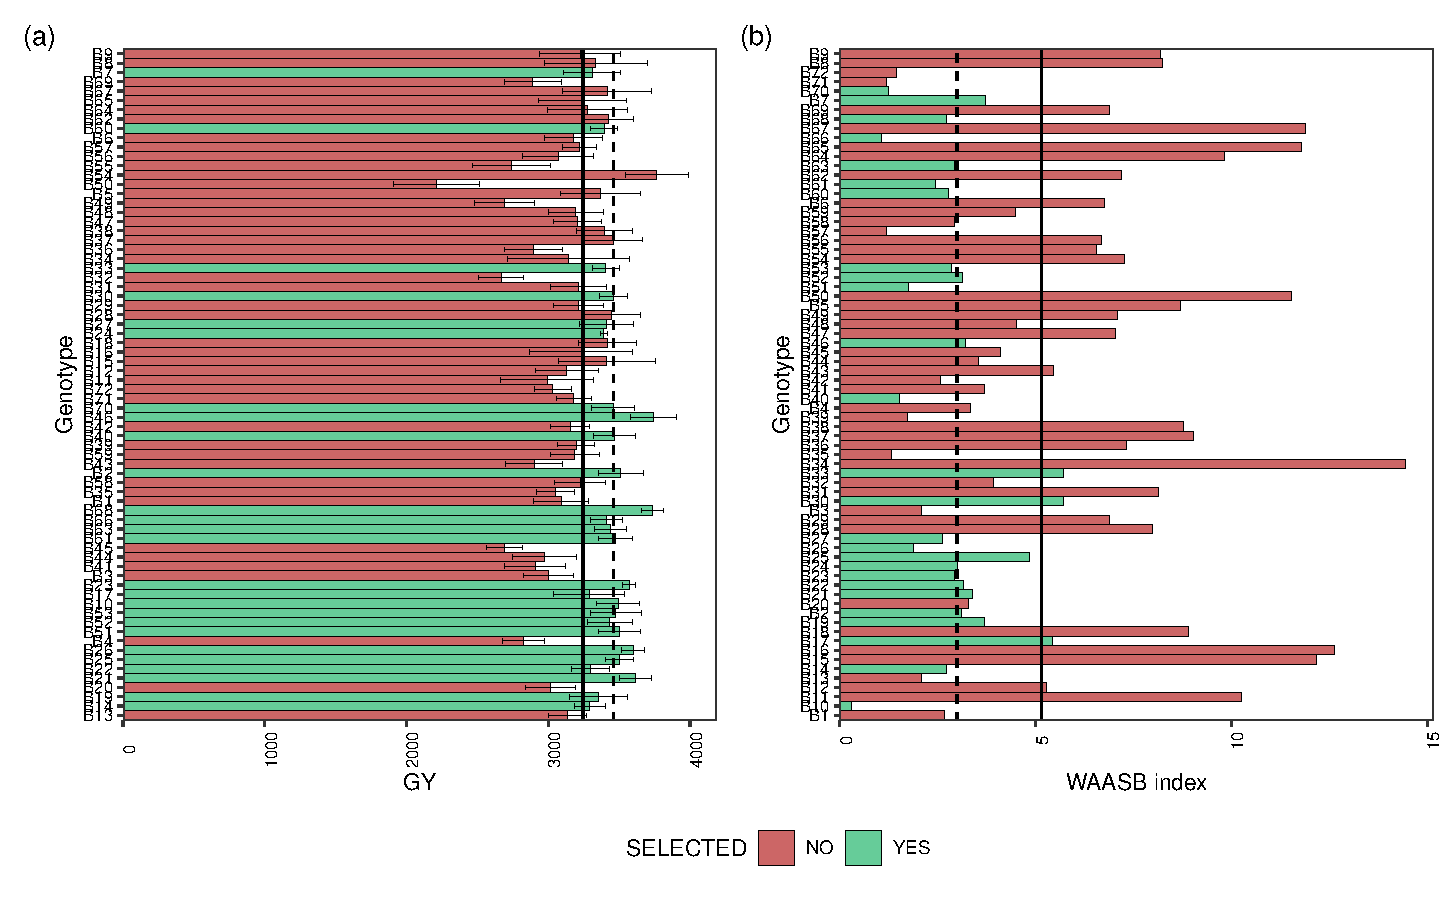
\includegraphics{figures/mod metan bb stab2-1} 

}

\caption{Mean performance (a) and stability (b) for grain yield (GY) of 72 Black beans genotypes. The vertical dashed and solid lines shows, respectivelly, the  mean of the selected genotype and the overall mean for both mean performance and WAASB index}\label{fig:mod metan bb stab2}
\end{figure}

Percentage (SD\_gain in \%) gain from the selected genotypes compared to
the general mean.

\begin{Shaded}
\begin{Highlighting}[]
\NormalTok{blups\_sel2 }\OtherTok{\textless{}{-}}
  \FunctionTok{gmd}\NormalTok{(waasb\_model\_bb, }\StringTok{"blupg"}\NormalTok{) }\SpecialCharTok{\%\textgreater{}\%}
  \FunctionTok{add\_cols}\NormalTok{(}\AttributeTok{SELECTED =} \FunctionTok{ifelse}\NormalTok{(GEN }\SpecialCharTok{\%in\%}\NormalTok{ selected}\SpecialCharTok{$}\NormalTok{Code, }\StringTok{"yes"}\NormalTok{, }\StringTok{"no"}\NormalTok{)) }\SpecialCharTok{\%\textgreater{}\%} 
\NormalTok{    dplyr}\SpecialCharTok{::}\FunctionTok{rename}\NormalTok{(}\AttributeTok{BLUPs\_sel =}\NormalTok{ yield) }\SpecialCharTok{\%\textgreater{}\%} 
  \FunctionTok{droplevels}\NormalTok{()}
\end{Highlighting}
\end{Shaded}

\begin{verbatim}
#> Class of the model: waasb
\end{verbatim}

\begin{verbatim}
#> Variable extracted: blupg
\end{verbatim}

\begin{Shaded}
\begin{Highlighting}[]
\NormalTok{blups\_sel\_mean2}\OtherTok{\textless{}{-}}
  \FunctionTok{gmd}\NormalTok{(waasb\_model\_bb, }\StringTok{"blupg"}\NormalTok{) }\SpecialCharTok{\%\textgreater{}\%}
  \FunctionTok{add\_cols}\NormalTok{(}\AttributeTok{SELECTED =} \FunctionTok{ifelse}\NormalTok{(GEN }\SpecialCharTok{\%in\%}\NormalTok{ selected}\SpecialCharTok{$}\NormalTok{Code, }\StringTok{"yes"}\NormalTok{, }\StringTok{"no"}\NormalTok{)) }\SpecialCharTok{\%\textgreater{}\%} 
  \FunctionTok{filter}\NormalTok{(SELECTED }\SpecialCharTok{==} \StringTok{"yes"}\NormalTok{) }\SpecialCharTok{\%\textgreater{}\%} 
\NormalTok{  dplyr}\SpecialCharTok{::}\FunctionTok{summarise}\NormalTok{(}\AttributeTok{mean\_GY =} \FunctionTok{mean}\NormalTok{(yield,}\AttributeTok{na.rm =} \ConstantTok{TRUE}\NormalTok{), }\AttributeTok{n =} \FunctionTok{n}\NormalTok{()) }
\end{Highlighting}
\end{Shaded}

\begin{verbatim}
#> Class of the model: waasb
#> Variable extracted: blupg
\end{verbatim}

\begin{Shaded}
\begin{Highlighting}[]
\NormalTok{SD\_blups}\OtherTok{\textless{}{-}} \FunctionTok{as\_tibble}\NormalTok{((blups\_sel\_mean2}\SpecialCharTok{$}\NormalTok{mean\_GY}\SpecialCharTok{/}\FunctionTok{mean}\NormalTok{(blups\_sel2}\SpecialCharTok{$}\NormalTok{BLUPs\_sel, }\AttributeTok{na.rm =}\NormalTok{ T)) }\SpecialCharTok{{-}}\DecValTok{1}\NormalTok{)}\SpecialCharTok{*}\DecValTok{100}
\NormalTok{SD\_WAASP}\OtherTok{\textless{}{-}} \FunctionTok{as\_tibble}\NormalTok{((waasb\_sel\_mean}\SpecialCharTok{$}\NormalTok{mean\_GY }\SpecialCharTok{/}\FunctionTok{mean}\NormalTok{(waasb\_sel}\SpecialCharTok{$}\NormalTok{WAASB\_sel, }\AttributeTok{na.rm =}\NormalTok{ T)) }\SpecialCharTok{{-}}\DecValTok{1}\NormalTok{)}\SpecialCharTok{*}\DecValTok{100}

\NormalTok{SD\_comb}\OtherTok{\textless{}{-}} \FunctionTok{full\_join}\NormalTok{(SD\_blups, SD\_WAASP, }\AttributeTok{by =} \StringTok{"value"}\NormalTok{) }\SpecialCharTok{\%\textgreater{}\%} 
\NormalTok{  dplyr}\SpecialCharTok{::}\FunctionTok{rename}\NormalTok{(}\AttributeTok{SD\_gain =}\NormalTok{ value) }\SpecialCharTok{\%\textgreater{}\%} 
\NormalTok{  tibble}\SpecialCharTok{::}\FunctionTok{add\_column}\NormalTok{(}\AttributeTok{Comp\_name =} \FunctionTok{c}\NormalTok{(}\StringTok{\textquotesingle{}BLUPs\textquotesingle{}}\NormalTok{, }\StringTok{\textquotesingle{}WAASB\textquotesingle{}}\NormalTok{)) }\SpecialCharTok{\%\textgreater{}\%} 
  \FunctionTok{relocate}\NormalTok{(Comp\_name)}

\NormalTok{SD\_comb}\SpecialCharTok{$}\NormalTok{n\_selected}\OtherTok{\textless{}{-}}\NormalTok{ blups\_sel\_mean2}\SpecialCharTok{$}\NormalTok{n}
\NormalTok{SD\_comb}
\end{Highlighting}
\end{Shaded}

\global\setlength{\Oldarrayrulewidth}{\arrayrulewidth}

\global\setlength{\Oldtabcolsep}{\tabcolsep}

\setlength{\tabcolsep}{0pt}

\renewcommand*{\arraystretch}{1.5}



\providecommand{\ascline}[3]{\noalign{\global\arrayrulewidth #1}\arrayrulecolor[HTML]{#2}\cline{#3}}

\begin{longtable}[c]{|p{0.96in}|p{0.75in}|p{0.86in}}



\ascline{1.5pt}{666666}{1-3}

\multicolumn{1}{>{\raggedright}m{\dimexpr 0.96in+0\tabcolsep}}{\textcolor[HTML]{000000}{\fontsize{9}{9}\selectfont{\global\setmainfont{Arial}{\textbf{Comp\_name}}}}} & \multicolumn{1}{>{\raggedleft}m{\dimexpr 0.75in+0\tabcolsep}}{\textcolor[HTML]{000000}{\fontsize{9}{9}\selectfont{\global\setmainfont{Arial}{\textbf{SD\_gain}}}}} & \multicolumn{1}{>{\raggedleft}m{\dimexpr 0.86in+0\tabcolsep}}{\textcolor[HTML]{000000}{\fontsize{9}{9}\selectfont{\global\setmainfont{Arial}{\textbf{n\_selected}}}}} \\

\ascline{0.75pt}{666666}{1-3}



\multicolumn{1}{>{\raggedright}m{\dimexpr 0.96in+0\tabcolsep}}{\textcolor[HTML]{999999}{\fontsize{9}{9}\selectfont{\global\setmainfont{Arial}{\textbf{character}}}}} & \multicolumn{1}{>{\raggedleft}m{\dimexpr 0.75in+0\tabcolsep}}{\textcolor[HTML]{999999}{\fontsize{9}{9}\selectfont{\global\setmainfont{Arial}{\textbf{numeric}}}}} & \multicolumn{1}{>{\raggedleft}m{\dimexpr 0.86in+0\tabcolsep}}{\textcolor[HTML]{999999}{\fontsize{9}{9}\selectfont{\global\setmainfont{Arial}{\textbf{integer}}}}} \\

\ascline{1.5pt}{666666}{1-3}\endfirsthead

\ascline{1.5pt}{666666}{1-3}

\multicolumn{1}{>{\raggedright}m{\dimexpr 0.96in+0\tabcolsep}}{\textcolor[HTML]{000000}{\fontsize{9}{9}\selectfont{\global\setmainfont{Arial}{\textbf{Comp\_name}}}}} & \multicolumn{1}{>{\raggedleft}m{\dimexpr 0.75in+0\tabcolsep}}{\textcolor[HTML]{000000}{\fontsize{9}{9}\selectfont{\global\setmainfont{Arial}{\textbf{SD\_gain}}}}} & \multicolumn{1}{>{\raggedleft}m{\dimexpr 0.86in+0\tabcolsep}}{\textcolor[HTML]{000000}{\fontsize{9}{9}\selectfont{\global\setmainfont{Arial}{\textbf{n\_selected}}}}} \\

\ascline{0.75pt}{666666}{1-3}



\multicolumn{1}{>{\raggedright}m{\dimexpr 0.96in+0\tabcolsep}}{\textcolor[HTML]{999999}{\fontsize{9}{9}\selectfont{\global\setmainfont{Arial}{\textbf{character}}}}} & \multicolumn{1}{>{\raggedleft}m{\dimexpr 0.75in+0\tabcolsep}}{\textcolor[HTML]{999999}{\fontsize{9}{9}\selectfont{\global\setmainfont{Arial}{\textbf{numeric}}}}} & \multicolumn{1}{>{\raggedleft}m{\dimexpr 0.86in+0\tabcolsep}}{\textcolor[HTML]{999999}{\fontsize{9}{9}\selectfont{\global\setmainfont{Arial}{\textbf{integer}}}}} \\

\ascline{1.5pt}{666666}{1-3}\endhead



\multicolumn{3}{>{\raggedright}m{\dimexpr 2.57in+4\tabcolsep}}{\textcolor[HTML]{000000}{\fontsize{9}{9}\selectfont{\global\setmainfont{Arial}{n:\ 2}}}} \\

\ascline{0.75pt}{666666}{1-3}\endfoot



\multicolumn{1}{>{\raggedright}m{\dimexpr 0.96in+0\tabcolsep}}{\textcolor[HTML]{000000}{\fontsize{9}{9}\selectfont{\global\setmainfont{Arial}{BLUPs}}}} & \multicolumn{1}{>{\raggedleft}m{\dimexpr 0.75in+0\tabcolsep}}{\textcolor[HTML]{000000}{\fontsize{9}{9}\selectfont{\global\setmainfont{Arial}{3.7}}}} & \multicolumn{1}{>{\raggedleft}m{\dimexpr 0.86in+0\tabcolsep}}{\textcolor[HTML]{000000}{\fontsize{9}{9}\selectfont{\global\setmainfont{Arial}{26}}}} \\

\ascline{0.75pt}{666666}{1-3}



\multicolumn{1}{>{\raggedright}m{\dimexpr 0.96in+0\tabcolsep}}{\textcolor[HTML]{000000}{\fontsize{9}{9}\selectfont{\global\setmainfont{Arial}{WAASB}}}} & \multicolumn{1}{>{\raggedleft}m{\dimexpr 0.75in+0\tabcolsep}}{\textcolor[HTML]{000000}{\fontsize{9}{9}\selectfont{\global\setmainfont{Arial}{-41.9}}}} & \multicolumn{1}{>{\raggedleft}m{\dimexpr 0.86in+0\tabcolsep}}{\textcolor[HTML]{000000}{\fontsize{9}{9}\selectfont{\global\setmainfont{Arial}{26}}}} \\

\ascline{1.5pt}{666666}{1-3}



\end{longtable}



\arrayrulecolor[HTML]{000000}

\global\setlength{\arrayrulewidth}{\Oldarrayrulewidth}

\global\setlength{\tabcolsep}{\Oldtabcolsep}

\renewcommand*{\arraystretch}{1}

\begin{Shaded}
\begin{Highlighting}[]
\NormalTok{blups\_sel2}\SpecialCharTok{$}\NormalTok{mean\_blup }\OtherTok{\textless{}{-}} \FunctionTok{mean}\NormalTok{(blups\_sel2}\SpecialCharTok{$}\NormalTok{BLUPs\_sel, }\AttributeTok{na.rm =}\NormalTok{ T)}
\NormalTok{waasb\_sel}\SpecialCharTok{$}\NormalTok{mean\_waasb }\OtherTok{\textless{}{-}} \FunctionTok{mean}\NormalTok{(waasb\_sel}\SpecialCharTok{$}\NormalTok{WAASB\_sel, }\AttributeTok{na.rm =}\NormalTok{ T)}

\CommentTok{\#str(waasb\_sel)}
\NormalTok{data\_comb}\OtherTok{\textless{}{-}} \FunctionTok{merge}\NormalTok{(blups\_sel2, waasb\_sel, }\AttributeTok{by =} \FunctionTok{c}\NormalTok{(}\StringTok{"GEN"}\NormalTok{, }\StringTok{"SELECTED"}\NormalTok{))}
\CommentTok{\#names(data\_comb)}
\DocumentationTok{\#\# SD for each genotype}
\NormalTok{data\_sel\_perc }\OtherTok{\textless{}{-}}\NormalTok{ data\_comb }\SpecialCharTok{\%\textgreater{}\%}
\NormalTok{ rowwise }\SpecialCharTok{\%\textgreater{}\%}
  \FunctionTok{mutate}\NormalTok{(}\AttributeTok{Perc\_blup\_gain =}\NormalTok{ ((BLUPs\_sel}\SpecialCharTok{/}\NormalTok{mean\_blup)}\SpecialCharTok{*}\DecValTok{100}\NormalTok{)}\SpecialCharTok{{-}}\DecValTok{100}\NormalTok{) }\SpecialCharTok{\%\textgreater{}\%} 
  \FunctionTok{mutate}\NormalTok{(}\AttributeTok{Perc\_WAASB\_gain =}\NormalTok{ ((WAASB\_sel}\SpecialCharTok{/}\NormalTok{mean\_waasb)}\SpecialCharTok{*}\DecValTok{100}\NormalTok{)}\SpecialCharTok{{-}}\DecValTok{100}\NormalTok{) }\SpecialCharTok{\%\textgreater{}\%} 
  \FunctionTok{as\_tibble}\NormalTok{()}

\CommentTok{\# data\_sel\_perc\_mean \textless{}{-} data\_sel\_perc \%\textgreater{}\% }
\CommentTok{\#   dplyr::filter(SELECTED  == "yes")}
\CommentTok{\# }
\CommentTok{\# mean(data\_sel\_perc\_mean$Perc\_blup\_gain)}

\ControlFlowTok{if}\NormalTok{ (knitr}\SpecialCharTok{::}\FunctionTok{is\_html\_output}\NormalTok{()) \{}
  
\FunctionTok{print\_table}\NormalTok{(data\_sel\_perc)}
  
\NormalTok{\}}\ControlFlowTok{else}\NormalTok{\{}
  
\NormalTok{data\_sel\_perc[,}\DecValTok{1}\SpecialCharTok{:}\DecValTok{7}\NormalTok{]}
\NormalTok{\}}
\end{Highlighting}
\end{Shaded}

\global\setlength{\Oldarrayrulewidth}{\arrayrulewidth}

\global\setlength{\Oldtabcolsep}{\tabcolsep}

\setlength{\tabcolsep}{0pt}

\renewcommand*{\arraystretch}{1.5}



\providecommand{\ascline}[3]{\noalign{\global\arrayrulewidth #1}\arrayrulecolor[HTML]{#2}\cline{#3}}

\begin{longtable}[c]{|p{0.77in}|p{0.88in}|p{0.86in}|p{0.87in}|p{0.93in}|p{0.99in}|p{1.14in}}



\ascline{1.5pt}{666666}{1-7}

\multicolumn{1}{>{\raggedright}m{\dimexpr 0.77in+0\tabcolsep}}{\textcolor[HTML]{000000}{\fontsize{9}{9}\selectfont{\global\setmainfont{Arial}{\textbf{GEN}}}}} & \multicolumn{1}{>{\raggedright}m{\dimexpr 0.88in+0\tabcolsep}}{\textcolor[HTML]{000000}{\fontsize{9}{9}\selectfont{\global\setmainfont{Arial}{\textbf{SELECTED}}}}} & \multicolumn{1}{>{\raggedleft}m{\dimexpr 0.86in+0\tabcolsep}}{\textcolor[HTML]{000000}{\fontsize{9}{9}\selectfont{\global\setmainfont{Arial}{\textbf{BLUPs\_sel}}}}} & \multicolumn{1}{>{\raggedleft}m{\dimexpr 0.87in+0\tabcolsep}}{\textcolor[HTML]{000000}{\fontsize{9}{9}\selectfont{\global\setmainfont{Arial}{\textbf{mean\_blup}}}}} & \multicolumn{1}{>{\raggedleft}m{\dimexpr 0.93in+0\tabcolsep}}{\textcolor[HTML]{000000}{\fontsize{9}{9}\selectfont{\global\setmainfont{Arial}{\textbf{WAASB\_sel}}}}} & \multicolumn{1}{>{\raggedleft}m{\dimexpr 0.99in+0\tabcolsep}}{\textcolor[HTML]{000000}{\fontsize{9}{9}\selectfont{\global\setmainfont{Arial}{\textbf{mean\_waasb}}}}} & \multicolumn{1}{>{\raggedleft}m{\dimexpr 1.14in+0\tabcolsep}}{\textcolor[HTML]{000000}{\fontsize{9}{9}\selectfont{\global\setmainfont{Arial}{\textbf{Perc\_blup\_gain}}}}} \\

\ascline{0.75pt}{666666}{1-7}



\multicolumn{1}{>{\raggedright}m{\dimexpr 0.77in+0\tabcolsep}}{\textcolor[HTML]{999999}{\fontsize{9}{9}\selectfont{\global\setmainfont{Arial}{\textbf{character}}}}} & \multicolumn{1}{>{\raggedright}m{\dimexpr 0.88in+0\tabcolsep}}{\textcolor[HTML]{999999}{\fontsize{9}{9}\selectfont{\global\setmainfont{Arial}{\textbf{character}}}}} & \multicolumn{1}{>{\raggedleft}m{\dimexpr 0.86in+0\tabcolsep}}{\textcolor[HTML]{999999}{\fontsize{9}{9}\selectfont{\global\setmainfont{Arial}{\textbf{numeric}}}}} & \multicolumn{1}{>{\raggedleft}m{\dimexpr 0.87in+0\tabcolsep}}{\textcolor[HTML]{999999}{\fontsize{9}{9}\selectfont{\global\setmainfont{Arial}{\textbf{numeric}}}}} & \multicolumn{1}{>{\raggedleft}m{\dimexpr 0.93in+0\tabcolsep}}{\textcolor[HTML]{999999}{\fontsize{9}{9}\selectfont{\global\setmainfont{Arial}{\textbf{numeric}}}}} & \multicolumn{1}{>{\raggedleft}m{\dimexpr 0.99in+0\tabcolsep}}{\textcolor[HTML]{999999}{\fontsize{9}{9}\selectfont{\global\setmainfont{Arial}{\textbf{numeric}}}}} & \multicolumn{1}{>{\raggedleft}m{\dimexpr 1.14in+0\tabcolsep}}{\textcolor[HTML]{999999}{\fontsize{9}{9}\selectfont{\global\setmainfont{Arial}{\textbf{numeric}}}}} \\

\ascline{1.5pt}{666666}{1-7}\endfirsthead

\ascline{1.5pt}{666666}{1-7}

\multicolumn{1}{>{\raggedright}m{\dimexpr 0.77in+0\tabcolsep}}{\textcolor[HTML]{000000}{\fontsize{9}{9}\selectfont{\global\setmainfont{Arial}{\textbf{GEN}}}}} & \multicolumn{1}{>{\raggedright}m{\dimexpr 0.88in+0\tabcolsep}}{\textcolor[HTML]{000000}{\fontsize{9}{9}\selectfont{\global\setmainfont{Arial}{\textbf{SELECTED}}}}} & \multicolumn{1}{>{\raggedleft}m{\dimexpr 0.86in+0\tabcolsep}}{\textcolor[HTML]{000000}{\fontsize{9}{9}\selectfont{\global\setmainfont{Arial}{\textbf{BLUPs\_sel}}}}} & \multicolumn{1}{>{\raggedleft}m{\dimexpr 0.87in+0\tabcolsep}}{\textcolor[HTML]{000000}{\fontsize{9}{9}\selectfont{\global\setmainfont{Arial}{\textbf{mean\_blup}}}}} & \multicolumn{1}{>{\raggedleft}m{\dimexpr 0.93in+0\tabcolsep}}{\textcolor[HTML]{000000}{\fontsize{9}{9}\selectfont{\global\setmainfont{Arial}{\textbf{WAASB\_sel}}}}} & \multicolumn{1}{>{\raggedleft}m{\dimexpr 0.99in+0\tabcolsep}}{\textcolor[HTML]{000000}{\fontsize{9}{9}\selectfont{\global\setmainfont{Arial}{\textbf{mean\_waasb}}}}} & \multicolumn{1}{>{\raggedleft}m{\dimexpr 1.14in+0\tabcolsep}}{\textcolor[HTML]{000000}{\fontsize{9}{9}\selectfont{\global\setmainfont{Arial}{\textbf{Perc\_blup\_gain}}}}} \\

\ascline{0.75pt}{666666}{1-7}



\multicolumn{1}{>{\raggedright}m{\dimexpr 0.77in+0\tabcolsep}}{\textcolor[HTML]{999999}{\fontsize{9}{9}\selectfont{\global\setmainfont{Arial}{\textbf{character}}}}} & \multicolumn{1}{>{\raggedright}m{\dimexpr 0.88in+0\tabcolsep}}{\textcolor[HTML]{999999}{\fontsize{9}{9}\selectfont{\global\setmainfont{Arial}{\textbf{character}}}}} & \multicolumn{1}{>{\raggedleft}m{\dimexpr 0.86in+0\tabcolsep}}{\textcolor[HTML]{999999}{\fontsize{9}{9}\selectfont{\global\setmainfont{Arial}{\textbf{numeric}}}}} & \multicolumn{1}{>{\raggedleft}m{\dimexpr 0.87in+0\tabcolsep}}{\textcolor[HTML]{999999}{\fontsize{9}{9}\selectfont{\global\setmainfont{Arial}{\textbf{numeric}}}}} & \multicolumn{1}{>{\raggedleft}m{\dimexpr 0.93in+0\tabcolsep}}{\textcolor[HTML]{999999}{\fontsize{9}{9}\selectfont{\global\setmainfont{Arial}{\textbf{numeric}}}}} & \multicolumn{1}{>{\raggedleft}m{\dimexpr 0.99in+0\tabcolsep}}{\textcolor[HTML]{999999}{\fontsize{9}{9}\selectfont{\global\setmainfont{Arial}{\textbf{numeric}}}}} & \multicolumn{1}{>{\raggedleft}m{\dimexpr 1.14in+0\tabcolsep}}{\textcolor[HTML]{999999}{\fontsize{9}{9}\selectfont{\global\setmainfont{Arial}{\textbf{numeric}}}}} \\

\ascline{1.5pt}{666666}{1-7}\endhead



\multicolumn{7}{>{\raggedright}m{\dimexpr 6.44in+12\tabcolsep}}{\textcolor[HTML]{000000}{\fontsize{9}{9}\selectfont{\global\setmainfont{Arial}{n:\ 72}}}} \\

\ascline{0.75pt}{666666}{1-7}\endfoot



\multicolumn{1}{>{\raggedright}m{\dimexpr 0.77in+0\tabcolsep}}{\textcolor[HTML]{000000}{\fontsize{9}{9}\selectfont{\global\setmainfont{Arial}{B1}}}} & \multicolumn{1}{>{\raggedright}m{\dimexpr 0.88in+0\tabcolsep}}{\textcolor[HTML]{000000}{\fontsize{9}{9}\selectfont{\global\setmainfont{Arial}{no}}}} & \multicolumn{1}{>{\raggedleft}m{\dimexpr 0.86in+0\tabcolsep}}{\textcolor[HTML]{000000}{\fontsize{9}{9}\selectfont{\global\setmainfont{Arial}{3,173.6}}}} & \multicolumn{1}{>{\raggedleft}m{\dimexpr 0.87in+0\tabcolsep}}{\textcolor[HTML]{000000}{\fontsize{9}{9}\selectfont{\global\setmainfont{Arial}{3,255.1}}}} & \multicolumn{1}{>{\raggedleft}m{\dimexpr 0.93in+0\tabcolsep}}{\textcolor[HTML]{000000}{\fontsize{9}{9}\selectfont{\global\setmainfont{Arial}{2.7}}}} & \multicolumn{1}{>{\raggedleft}m{\dimexpr 0.99in+0\tabcolsep}}{\textcolor[HTML]{000000}{\fontsize{9}{9}\selectfont{\global\setmainfont{Arial}{5.2}}}} & \multicolumn{1}{>{\raggedleft}m{\dimexpr 1.14in+0\tabcolsep}}{\textcolor[HTML]{000000}{\fontsize{9}{9}\selectfont{\global\setmainfont{Arial}{-2.5}}}} \\

\ascline{0.75pt}{666666}{1-7}



\multicolumn{1}{>{\raggedright}m{\dimexpr 0.77in+0\tabcolsep}}{\textcolor[HTML]{000000}{\fontsize{9}{9}\selectfont{\global\setmainfont{Arial}{B10}}}} & \multicolumn{1}{>{\raggedright}m{\dimexpr 0.88in+0\tabcolsep}}{\textcolor[HTML]{000000}{\fontsize{9}{9}\selectfont{\global\setmainfont{Arial}{yes}}}} & \multicolumn{1}{>{\raggedleft}m{\dimexpr 0.86in+0\tabcolsep}}{\textcolor[HTML]{000000}{\fontsize{9}{9}\selectfont{\global\setmainfont{Arial}{3,391.1}}}} & \multicolumn{1}{>{\raggedleft}m{\dimexpr 0.87in+0\tabcolsep}}{\textcolor[HTML]{000000}{\fontsize{9}{9}\selectfont{\global\setmainfont{Arial}{3,255.1}}}} & \multicolumn{1}{>{\raggedleft}m{\dimexpr 0.93in+0\tabcolsep}}{\textcolor[HTML]{000000}{\fontsize{9}{9}\selectfont{\global\setmainfont{Arial}{0.3}}}} & \multicolumn{1}{>{\raggedleft}m{\dimexpr 0.99in+0\tabcolsep}}{\textcolor[HTML]{000000}{\fontsize{9}{9}\selectfont{\global\setmainfont{Arial}{5.2}}}} & \multicolumn{1}{>{\raggedleft}m{\dimexpr 1.14in+0\tabcolsep}}{\textcolor[HTML]{000000}{\fontsize{9}{9}\selectfont{\global\setmainfont{Arial}{4.2}}}} \\

\ascline{0.75pt}{666666}{1-7}



\multicolumn{1}{>{\raggedright}m{\dimexpr 0.77in+0\tabcolsep}}{\textcolor[HTML]{000000}{\fontsize{9}{9}\selectfont{\global\setmainfont{Arial}{B11}}}} & \multicolumn{1}{>{\raggedright}m{\dimexpr 0.88in+0\tabcolsep}}{\textcolor[HTML]{000000}{\fontsize{9}{9}\selectfont{\global\setmainfont{Arial}{no}}}} & \multicolumn{1}{>{\raggedleft}m{\dimexpr 0.86in+0\tabcolsep}}{\textcolor[HTML]{000000}{\fontsize{9}{9}\selectfont{\global\setmainfont{Arial}{3,110.5}}}} & \multicolumn{1}{>{\raggedleft}m{\dimexpr 0.87in+0\tabcolsep}}{\textcolor[HTML]{000000}{\fontsize{9}{9}\selectfont{\global\setmainfont{Arial}{3,255.1}}}} & \multicolumn{1}{>{\raggedleft}m{\dimexpr 0.93in+0\tabcolsep}}{\textcolor[HTML]{000000}{\fontsize{9}{9}\selectfont{\global\setmainfont{Arial}{10.3}}}} & \multicolumn{1}{>{\raggedleft}m{\dimexpr 0.99in+0\tabcolsep}}{\textcolor[HTML]{000000}{\fontsize{9}{9}\selectfont{\global\setmainfont{Arial}{5.2}}}} & \multicolumn{1}{>{\raggedleft}m{\dimexpr 1.14in+0\tabcolsep}}{\textcolor[HTML]{000000}{\fontsize{9}{9}\selectfont{\global\setmainfont{Arial}{-4.4}}}} \\

\ascline{0.75pt}{666666}{1-7}



\multicolumn{1}{>{\raggedright}m{\dimexpr 0.77in+0\tabcolsep}}{\textcolor[HTML]{000000}{\fontsize{9}{9}\selectfont{\global\setmainfont{Arial}{B12}}}} & \multicolumn{1}{>{\raggedright}m{\dimexpr 0.88in+0\tabcolsep}}{\textcolor[HTML]{000000}{\fontsize{9}{9}\selectfont{\global\setmainfont{Arial}{no}}}} & \multicolumn{1}{>{\raggedleft}m{\dimexpr 0.86in+0\tabcolsep}}{\textcolor[HTML]{000000}{\fontsize{9}{9}\selectfont{\global\setmainfont{Arial}{3,185.4}}}} & \multicolumn{1}{>{\raggedleft}m{\dimexpr 0.87in+0\tabcolsep}}{\textcolor[HTML]{000000}{\fontsize{9}{9}\selectfont{\global\setmainfont{Arial}{3,255.1}}}} & \multicolumn{1}{>{\raggedleft}m{\dimexpr 0.93in+0\tabcolsep}}{\textcolor[HTML]{000000}{\fontsize{9}{9}\selectfont{\global\setmainfont{Arial}{5.3}}}} & \multicolumn{1}{>{\raggedleft}m{\dimexpr 0.99in+0\tabcolsep}}{\textcolor[HTML]{000000}{\fontsize{9}{9}\selectfont{\global\setmainfont{Arial}{5.2}}}} & \multicolumn{1}{>{\raggedleft}m{\dimexpr 1.14in+0\tabcolsep}}{\textcolor[HTML]{000000}{\fontsize{9}{9}\selectfont{\global\setmainfont{Arial}{-2.1}}}} \\

\ascline{0.75pt}{666666}{1-7}



\multicolumn{1}{>{\raggedright}m{\dimexpr 0.77in+0\tabcolsep}}{\textcolor[HTML]{000000}{\fontsize{9}{9}\selectfont{\global\setmainfont{Arial}{B13}}}} & \multicolumn{1}{>{\raggedright}m{\dimexpr 0.88in+0\tabcolsep}}{\textcolor[HTML]{000000}{\fontsize{9}{9}\selectfont{\global\setmainfont{Arial}{no}}}} & \multicolumn{1}{>{\raggedleft}m{\dimexpr 0.86in+0\tabcolsep}}{\textcolor[HTML]{000000}{\fontsize{9}{9}\selectfont{\global\setmainfont{Arial}{3,197.5}}}} & \multicolumn{1}{>{\raggedleft}m{\dimexpr 0.87in+0\tabcolsep}}{\textcolor[HTML]{000000}{\fontsize{9}{9}\selectfont{\global\setmainfont{Arial}{3,255.1}}}} & \multicolumn{1}{>{\raggedleft}m{\dimexpr 0.93in+0\tabcolsep}}{\textcolor[HTML]{000000}{\fontsize{9}{9}\selectfont{\global\setmainfont{Arial}{2.1}}}} & \multicolumn{1}{>{\raggedleft}m{\dimexpr 0.99in+0\tabcolsep}}{\textcolor[HTML]{000000}{\fontsize{9}{9}\selectfont{\global\setmainfont{Arial}{5.2}}}} & \multicolumn{1}{>{\raggedleft}m{\dimexpr 1.14in+0\tabcolsep}}{\textcolor[HTML]{000000}{\fontsize{9}{9}\selectfont{\global\setmainfont{Arial}{-1.8}}}} \\

\ascline{0.75pt}{666666}{1-7}



\multicolumn{1}{>{\raggedright}m{\dimexpr 0.77in+0\tabcolsep}}{\textcolor[HTML]{000000}{\fontsize{9}{9}\selectfont{\global\setmainfont{Arial}{B14}}}} & \multicolumn{1}{>{\raggedright}m{\dimexpr 0.88in+0\tabcolsep}}{\textcolor[HTML]{000000}{\fontsize{9}{9}\selectfont{\global\setmainfont{Arial}{yes}}}} & \multicolumn{1}{>{\raggedleft}m{\dimexpr 0.86in+0\tabcolsep}}{\textcolor[HTML]{000000}{\fontsize{9}{9}\selectfont{\global\setmainfont{Arial}{3,282.6}}}} & \multicolumn{1}{>{\raggedleft}m{\dimexpr 0.87in+0\tabcolsep}}{\textcolor[HTML]{000000}{\fontsize{9}{9}\selectfont{\global\setmainfont{Arial}{3,255.1}}}} & \multicolumn{1}{>{\raggedleft}m{\dimexpr 0.93in+0\tabcolsep}}{\textcolor[HTML]{000000}{\fontsize{9}{9}\selectfont{\global\setmainfont{Arial}{2.7}}}} & \multicolumn{1}{>{\raggedleft}m{\dimexpr 0.99in+0\tabcolsep}}{\textcolor[HTML]{000000}{\fontsize{9}{9}\selectfont{\global\setmainfont{Arial}{5.2}}}} & \multicolumn{1}{>{\raggedleft}m{\dimexpr 1.14in+0\tabcolsep}}{\textcolor[HTML]{000000}{\fontsize{9}{9}\selectfont{\global\setmainfont{Arial}{0.8}}}} \\

\ascline{0.75pt}{666666}{1-7}



\multicolumn{1}{>{\raggedright}m{\dimexpr 0.77in+0\tabcolsep}}{\textcolor[HTML]{000000}{\fontsize{9}{9}\selectfont{\global\setmainfont{Arial}{B15}}}} & \multicolumn{1}{>{\raggedright}m{\dimexpr 0.88in+0\tabcolsep}}{\textcolor[HTML]{000000}{\fontsize{9}{9}\selectfont{\global\setmainfont{Arial}{no}}}} & \multicolumn{1}{>{\raggedleft}m{\dimexpr 0.86in+0\tabcolsep}}{\textcolor[HTML]{000000}{\fontsize{9}{9}\selectfont{\global\setmainfont{Arial}{3,337.8}}}} & \multicolumn{1}{>{\raggedleft}m{\dimexpr 0.87in+0\tabcolsep}}{\textcolor[HTML]{000000}{\fontsize{9}{9}\selectfont{\global\setmainfont{Arial}{3,255.1}}}} & \multicolumn{1}{>{\raggedleft}m{\dimexpr 0.93in+0\tabcolsep}}{\textcolor[HTML]{000000}{\fontsize{9}{9}\selectfont{\global\setmainfont{Arial}{12.2}}}} & \multicolumn{1}{>{\raggedleft}m{\dimexpr 0.99in+0\tabcolsep}}{\textcolor[HTML]{000000}{\fontsize{9}{9}\selectfont{\global\setmainfont{Arial}{5.2}}}} & \multicolumn{1}{>{\raggedleft}m{\dimexpr 1.14in+0\tabcolsep}}{\textcolor[HTML]{000000}{\fontsize{9}{9}\selectfont{\global\setmainfont{Arial}{2.5}}}} \\

\ascline{0.75pt}{666666}{1-7}



\multicolumn{1}{>{\raggedright}m{\dimexpr 0.77in+0\tabcolsep}}{\textcolor[HTML]{000000}{\fontsize{9}{9}\selectfont{\global\setmainfont{Arial}{B16}}}} & \multicolumn{1}{>{\raggedright}m{\dimexpr 0.88in+0\tabcolsep}}{\textcolor[HTML]{000000}{\fontsize{9}{9}\selectfont{\global\setmainfont{Arial}{no}}}} & \multicolumn{1}{>{\raggedleft}m{\dimexpr 0.86in+0\tabcolsep}}{\textcolor[HTML]{000000}{\fontsize{9}{9}\selectfont{\global\setmainfont{Arial}{3,240.1}}}} & \multicolumn{1}{>{\raggedleft}m{\dimexpr 0.87in+0\tabcolsep}}{\textcolor[HTML]{000000}{\fontsize{9}{9}\selectfont{\global\setmainfont{Arial}{3,255.1}}}} & \multicolumn{1}{>{\raggedleft}m{\dimexpr 0.93in+0\tabcolsep}}{\textcolor[HTML]{000000}{\fontsize{9}{9}\selectfont{\global\setmainfont{Arial}{12.6}}}} & \multicolumn{1}{>{\raggedleft}m{\dimexpr 0.99in+0\tabcolsep}}{\textcolor[HTML]{000000}{\fontsize{9}{9}\selectfont{\global\setmainfont{Arial}{5.2}}}} & \multicolumn{1}{>{\raggedleft}m{\dimexpr 1.14in+0\tabcolsep}}{\textcolor[HTML]{000000}{\fontsize{9}{9}\selectfont{\global\setmainfont{Arial}{-0.5}}}} \\

\ascline{0.75pt}{666666}{1-7}



\multicolumn{1}{>{\raggedright}m{\dimexpr 0.77in+0\tabcolsep}}{\textcolor[HTML]{000000}{\fontsize{9}{9}\selectfont{\global\setmainfont{Arial}{B17}}}} & \multicolumn{1}{>{\raggedright}m{\dimexpr 0.88in+0\tabcolsep}}{\textcolor[HTML]{000000}{\fontsize{9}{9}\selectfont{\global\setmainfont{Arial}{yes}}}} & \multicolumn{1}{>{\raggedleft}m{\dimexpr 0.86in+0\tabcolsep}}{\textcolor[HTML]{000000}{\fontsize{9}{9}\selectfont{\global\setmainfont{Arial}{3,281.1}}}} & \multicolumn{1}{>{\raggedleft}m{\dimexpr 0.87in+0\tabcolsep}}{\textcolor[HTML]{000000}{\fontsize{9}{9}\selectfont{\global\setmainfont{Arial}{3,255.1}}}} & \multicolumn{1}{>{\raggedleft}m{\dimexpr 0.93in+0\tabcolsep}}{\textcolor[HTML]{000000}{\fontsize{9}{9}\selectfont{\global\setmainfont{Arial}{5.4}}}} & \multicolumn{1}{>{\raggedleft}m{\dimexpr 0.99in+0\tabcolsep}}{\textcolor[HTML]{000000}{\fontsize{9}{9}\selectfont{\global\setmainfont{Arial}{5.2}}}} & \multicolumn{1}{>{\raggedleft}m{\dimexpr 1.14in+0\tabcolsep}}{\textcolor[HTML]{000000}{\fontsize{9}{9}\selectfont{\global\setmainfont{Arial}{0.8}}}} \\

\ascline{1.5pt}{666666}{1-7}



\end{longtable}



\arrayrulecolor[HTML]{000000}

\global\setlength{\arrayrulewidth}{\Oldarrayrulewidth}

\global\setlength{\tabcolsep}{\Oldtabcolsep}

\renewcommand*{\arraystretch}{1}

\begin{Shaded}
\begin{Highlighting}[]
\NormalTok{data\_sel\_perc}\OtherTok{\textless{}{-}}\NormalTok{ data\_sel\_perc }\SpecialCharTok{\%\textgreater{}\%} 
\NormalTok{  dplyr}\SpecialCharTok{::}\FunctionTok{relocate}\NormalTok{(GEN,SELECTED,BLUPs\_sel,mean\_blup,Perc\_blup\_gain,}
\NormalTok{                 WAASB\_sel,mean\_waasb ,Perc\_WAASB\_gain)}

\CommentTok{\#write.xlsx(data\_sel\_perc, "./data/sel\_SD\_bb\_2.xlsx")}

\NormalTok{data\_sel\_perc2 }\OtherTok{\textless{}{-}}\NormalTok{ data\_sel\_perc }\SpecialCharTok{\%\textgreater{}\%} 
\NormalTok{  dplyr}\SpecialCharTok{::}\FunctionTok{select}\NormalTok{(GEN,SELECTED, BLUPs\_sel, WAASB\_sel, Perc\_blup\_gain, Perc\_WAASB\_gain)}

\NormalTok{data\_sel\_perc2}
\end{Highlighting}
\end{Shaded}

\global\setlength{\Oldarrayrulewidth}{\arrayrulewidth}

\global\setlength{\Oldtabcolsep}{\tabcolsep}

\setlength{\tabcolsep}{0pt}

\renewcommand*{\arraystretch}{1.5}



\providecommand{\ascline}[3]{\noalign{\global\arrayrulewidth #1}\arrayrulecolor[HTML]{#2}\cline{#3}}

\begin{longtable}[c]{|p{0.77in}|p{0.88in}|p{0.86in}|p{0.93in}|p{1.14in}|p{1.35in}}



\ascline{1.5pt}{666666}{1-6}

\multicolumn{1}{>{\raggedright}m{\dimexpr 0.77in+0\tabcolsep}}{\textcolor[HTML]{000000}{\fontsize{9}{9}\selectfont{\global\setmainfont{Arial}{\textbf{GEN}}}}} & \multicolumn{1}{>{\raggedright}m{\dimexpr 0.88in+0\tabcolsep}}{\textcolor[HTML]{000000}{\fontsize{9}{9}\selectfont{\global\setmainfont{Arial}{\textbf{SELECTED}}}}} & \multicolumn{1}{>{\raggedleft}m{\dimexpr 0.86in+0\tabcolsep}}{\textcolor[HTML]{000000}{\fontsize{9}{9}\selectfont{\global\setmainfont{Arial}{\textbf{BLUPs\_sel}}}}} & \multicolumn{1}{>{\raggedleft}m{\dimexpr 0.93in+0\tabcolsep}}{\textcolor[HTML]{000000}{\fontsize{9}{9}\selectfont{\global\setmainfont{Arial}{\textbf{WAASB\_sel}}}}} & \multicolumn{1}{>{\raggedleft}m{\dimexpr 1.14in+0\tabcolsep}}{\textcolor[HTML]{000000}{\fontsize{9}{9}\selectfont{\global\setmainfont{Arial}{\textbf{Perc\_blup\_gain}}}}} & \multicolumn{1}{>{\raggedleft}m{\dimexpr 1.35in+0\tabcolsep}}{\textcolor[HTML]{000000}{\fontsize{9}{9}\selectfont{\global\setmainfont{Arial}{\textbf{Perc\_WAASB\_gain}}}}} \\

\ascline{0.75pt}{666666}{1-6}



\multicolumn{1}{>{\raggedright}m{\dimexpr 0.77in+0\tabcolsep}}{\textcolor[HTML]{999999}{\fontsize{9}{9}\selectfont{\global\setmainfont{Arial}{\textbf{character}}}}} & \multicolumn{1}{>{\raggedright}m{\dimexpr 0.88in+0\tabcolsep}}{\textcolor[HTML]{999999}{\fontsize{9}{9}\selectfont{\global\setmainfont{Arial}{\textbf{character}}}}} & \multicolumn{1}{>{\raggedleft}m{\dimexpr 0.86in+0\tabcolsep}}{\textcolor[HTML]{999999}{\fontsize{9}{9}\selectfont{\global\setmainfont{Arial}{\textbf{numeric}}}}} & \multicolumn{1}{>{\raggedleft}m{\dimexpr 0.93in+0\tabcolsep}}{\textcolor[HTML]{999999}{\fontsize{9}{9}\selectfont{\global\setmainfont{Arial}{\textbf{numeric}}}}} & \multicolumn{1}{>{\raggedleft}m{\dimexpr 1.14in+0\tabcolsep}}{\textcolor[HTML]{999999}{\fontsize{9}{9}\selectfont{\global\setmainfont{Arial}{\textbf{numeric}}}}} & \multicolumn{1}{>{\raggedleft}m{\dimexpr 1.35in+0\tabcolsep}}{\textcolor[HTML]{999999}{\fontsize{9}{9}\selectfont{\global\setmainfont{Arial}{\textbf{numeric}}}}} \\

\ascline{1.5pt}{666666}{1-6}\endfirsthead

\ascline{1.5pt}{666666}{1-6}

\multicolumn{1}{>{\raggedright}m{\dimexpr 0.77in+0\tabcolsep}}{\textcolor[HTML]{000000}{\fontsize{9}{9}\selectfont{\global\setmainfont{Arial}{\textbf{GEN}}}}} & \multicolumn{1}{>{\raggedright}m{\dimexpr 0.88in+0\tabcolsep}}{\textcolor[HTML]{000000}{\fontsize{9}{9}\selectfont{\global\setmainfont{Arial}{\textbf{SELECTED}}}}} & \multicolumn{1}{>{\raggedleft}m{\dimexpr 0.86in+0\tabcolsep}}{\textcolor[HTML]{000000}{\fontsize{9}{9}\selectfont{\global\setmainfont{Arial}{\textbf{BLUPs\_sel}}}}} & \multicolumn{1}{>{\raggedleft}m{\dimexpr 0.93in+0\tabcolsep}}{\textcolor[HTML]{000000}{\fontsize{9}{9}\selectfont{\global\setmainfont{Arial}{\textbf{WAASB\_sel}}}}} & \multicolumn{1}{>{\raggedleft}m{\dimexpr 1.14in+0\tabcolsep}}{\textcolor[HTML]{000000}{\fontsize{9}{9}\selectfont{\global\setmainfont{Arial}{\textbf{Perc\_blup\_gain}}}}} & \multicolumn{1}{>{\raggedleft}m{\dimexpr 1.35in+0\tabcolsep}}{\textcolor[HTML]{000000}{\fontsize{9}{9}\selectfont{\global\setmainfont{Arial}{\textbf{Perc\_WAASB\_gain}}}}} \\

\ascline{0.75pt}{666666}{1-6}



\multicolumn{1}{>{\raggedright}m{\dimexpr 0.77in+0\tabcolsep}}{\textcolor[HTML]{999999}{\fontsize{9}{9}\selectfont{\global\setmainfont{Arial}{\textbf{character}}}}} & \multicolumn{1}{>{\raggedright}m{\dimexpr 0.88in+0\tabcolsep}}{\textcolor[HTML]{999999}{\fontsize{9}{9}\selectfont{\global\setmainfont{Arial}{\textbf{character}}}}} & \multicolumn{1}{>{\raggedleft}m{\dimexpr 0.86in+0\tabcolsep}}{\textcolor[HTML]{999999}{\fontsize{9}{9}\selectfont{\global\setmainfont{Arial}{\textbf{numeric}}}}} & \multicolumn{1}{>{\raggedleft}m{\dimexpr 0.93in+0\tabcolsep}}{\textcolor[HTML]{999999}{\fontsize{9}{9}\selectfont{\global\setmainfont{Arial}{\textbf{numeric}}}}} & \multicolumn{1}{>{\raggedleft}m{\dimexpr 1.14in+0\tabcolsep}}{\textcolor[HTML]{999999}{\fontsize{9}{9}\selectfont{\global\setmainfont{Arial}{\textbf{numeric}}}}} & \multicolumn{1}{>{\raggedleft}m{\dimexpr 1.35in+0\tabcolsep}}{\textcolor[HTML]{999999}{\fontsize{9}{9}\selectfont{\global\setmainfont{Arial}{\textbf{numeric}}}}} \\

\ascline{1.5pt}{666666}{1-6}\endhead



\multicolumn{6}{>{\raggedright}m{\dimexpr 5.93in+10\tabcolsep}}{\textcolor[HTML]{000000}{\fontsize{9}{9}\selectfont{\global\setmainfont{Arial}{n:\ 72}}}} \\

\ascline{0.75pt}{666666}{1-6}\endfoot



\multicolumn{1}{>{\raggedright}m{\dimexpr 0.77in+0\tabcolsep}}{\textcolor[HTML]{000000}{\fontsize{9}{9}\selectfont{\global\setmainfont{Arial}{B1}}}} & \multicolumn{1}{>{\raggedright}m{\dimexpr 0.88in+0\tabcolsep}}{\textcolor[HTML]{000000}{\fontsize{9}{9}\selectfont{\global\setmainfont{Arial}{no}}}} & \multicolumn{1}{>{\raggedleft}m{\dimexpr 0.86in+0\tabcolsep}}{\textcolor[HTML]{000000}{\fontsize{9}{9}\selectfont{\global\setmainfont{Arial}{3,173.6}}}} & \multicolumn{1}{>{\raggedleft}m{\dimexpr 0.93in+0\tabcolsep}}{\textcolor[HTML]{000000}{\fontsize{9}{9}\selectfont{\global\setmainfont{Arial}{2.7}}}} & \multicolumn{1}{>{\raggedleft}m{\dimexpr 1.14in+0\tabcolsep}}{\textcolor[HTML]{000000}{\fontsize{9}{9}\selectfont{\global\setmainfont{Arial}{-2.5}}}} & \multicolumn{1}{>{\raggedleft}m{\dimexpr 1.35in+0\tabcolsep}}{\textcolor[HTML]{000000}{\fontsize{9}{9}\selectfont{\global\setmainfont{Arial}{-48.3}}}} \\

\ascline{0.75pt}{666666}{1-6}



\multicolumn{1}{>{\raggedright}m{\dimexpr 0.77in+0\tabcolsep}}{\textcolor[HTML]{000000}{\fontsize{9}{9}\selectfont{\global\setmainfont{Arial}{B10}}}} & \multicolumn{1}{>{\raggedright}m{\dimexpr 0.88in+0\tabcolsep}}{\textcolor[HTML]{000000}{\fontsize{9}{9}\selectfont{\global\setmainfont{Arial}{yes}}}} & \multicolumn{1}{>{\raggedleft}m{\dimexpr 0.86in+0\tabcolsep}}{\textcolor[HTML]{000000}{\fontsize{9}{9}\selectfont{\global\setmainfont{Arial}{3,391.1}}}} & \multicolumn{1}{>{\raggedleft}m{\dimexpr 0.93in+0\tabcolsep}}{\textcolor[HTML]{000000}{\fontsize{9}{9}\selectfont{\global\setmainfont{Arial}{0.3}}}} & \multicolumn{1}{>{\raggedleft}m{\dimexpr 1.14in+0\tabcolsep}}{\textcolor[HTML]{000000}{\fontsize{9}{9}\selectfont{\global\setmainfont{Arial}{4.2}}}} & \multicolumn{1}{>{\raggedleft}m{\dimexpr 1.35in+0\tabcolsep}}{\textcolor[HTML]{000000}{\fontsize{9}{9}\selectfont{\global\setmainfont{Arial}{-94.2}}}} \\

\ascline{0.75pt}{666666}{1-6}



\multicolumn{1}{>{\raggedright}m{\dimexpr 0.77in+0\tabcolsep}}{\textcolor[HTML]{000000}{\fontsize{9}{9}\selectfont{\global\setmainfont{Arial}{B11}}}} & \multicolumn{1}{>{\raggedright}m{\dimexpr 0.88in+0\tabcolsep}}{\textcolor[HTML]{000000}{\fontsize{9}{9}\selectfont{\global\setmainfont{Arial}{no}}}} & \multicolumn{1}{>{\raggedleft}m{\dimexpr 0.86in+0\tabcolsep}}{\textcolor[HTML]{000000}{\fontsize{9}{9}\selectfont{\global\setmainfont{Arial}{3,110.5}}}} & \multicolumn{1}{>{\raggedleft}m{\dimexpr 0.93in+0\tabcolsep}}{\textcolor[HTML]{000000}{\fontsize{9}{9}\selectfont{\global\setmainfont{Arial}{10.3}}}} & \multicolumn{1}{>{\raggedleft}m{\dimexpr 1.14in+0\tabcolsep}}{\textcolor[HTML]{000000}{\fontsize{9}{9}\selectfont{\global\setmainfont{Arial}{-4.4}}}} & \multicolumn{1}{>{\raggedleft}m{\dimexpr 1.35in+0\tabcolsep}}{\textcolor[HTML]{000000}{\fontsize{9}{9}\selectfont{\global\setmainfont{Arial}{99.3}}}} \\

\ascline{0.75pt}{666666}{1-6}



\multicolumn{1}{>{\raggedright}m{\dimexpr 0.77in+0\tabcolsep}}{\textcolor[HTML]{000000}{\fontsize{9}{9}\selectfont{\global\setmainfont{Arial}{B12}}}} & \multicolumn{1}{>{\raggedright}m{\dimexpr 0.88in+0\tabcolsep}}{\textcolor[HTML]{000000}{\fontsize{9}{9}\selectfont{\global\setmainfont{Arial}{no}}}} & \multicolumn{1}{>{\raggedleft}m{\dimexpr 0.86in+0\tabcolsep}}{\textcolor[HTML]{000000}{\fontsize{9}{9}\selectfont{\global\setmainfont{Arial}{3,185.4}}}} & \multicolumn{1}{>{\raggedleft}m{\dimexpr 0.93in+0\tabcolsep}}{\textcolor[HTML]{000000}{\fontsize{9}{9}\selectfont{\global\setmainfont{Arial}{5.3}}}} & \multicolumn{1}{>{\raggedleft}m{\dimexpr 1.14in+0\tabcolsep}}{\textcolor[HTML]{000000}{\fontsize{9}{9}\selectfont{\global\setmainfont{Arial}{-2.1}}}} & \multicolumn{1}{>{\raggedleft}m{\dimexpr 1.35in+0\tabcolsep}}{\textcolor[HTML]{000000}{\fontsize{9}{9}\selectfont{\global\setmainfont{Arial}{2.7}}}} \\

\ascline{0.75pt}{666666}{1-6}



\multicolumn{1}{>{\raggedright}m{\dimexpr 0.77in+0\tabcolsep}}{\textcolor[HTML]{000000}{\fontsize{9}{9}\selectfont{\global\setmainfont{Arial}{B13}}}} & \multicolumn{1}{>{\raggedright}m{\dimexpr 0.88in+0\tabcolsep}}{\textcolor[HTML]{000000}{\fontsize{9}{9}\selectfont{\global\setmainfont{Arial}{no}}}} & \multicolumn{1}{>{\raggedleft}m{\dimexpr 0.86in+0\tabcolsep}}{\textcolor[HTML]{000000}{\fontsize{9}{9}\selectfont{\global\setmainfont{Arial}{3,197.5}}}} & \multicolumn{1}{>{\raggedleft}m{\dimexpr 0.93in+0\tabcolsep}}{\textcolor[HTML]{000000}{\fontsize{9}{9}\selectfont{\global\setmainfont{Arial}{2.1}}}} & \multicolumn{1}{>{\raggedleft}m{\dimexpr 1.14in+0\tabcolsep}}{\textcolor[HTML]{000000}{\fontsize{9}{9}\selectfont{\global\setmainfont{Arial}{-1.8}}}} & \multicolumn{1}{>{\raggedleft}m{\dimexpr 1.35in+0\tabcolsep}}{\textcolor[HTML]{000000}{\fontsize{9}{9}\selectfont{\global\setmainfont{Arial}{-59.6}}}} \\

\ascline{0.75pt}{666666}{1-6}



\multicolumn{1}{>{\raggedright}m{\dimexpr 0.77in+0\tabcolsep}}{\textcolor[HTML]{000000}{\fontsize{9}{9}\selectfont{\global\setmainfont{Arial}{B14}}}} & \multicolumn{1}{>{\raggedright}m{\dimexpr 0.88in+0\tabcolsep}}{\textcolor[HTML]{000000}{\fontsize{9}{9}\selectfont{\global\setmainfont{Arial}{yes}}}} & \multicolumn{1}{>{\raggedleft}m{\dimexpr 0.86in+0\tabcolsep}}{\textcolor[HTML]{000000}{\fontsize{9}{9}\selectfont{\global\setmainfont{Arial}{3,282.6}}}} & \multicolumn{1}{>{\raggedleft}m{\dimexpr 0.93in+0\tabcolsep}}{\textcolor[HTML]{000000}{\fontsize{9}{9}\selectfont{\global\setmainfont{Arial}{2.7}}}} & \multicolumn{1}{>{\raggedleft}m{\dimexpr 1.14in+0\tabcolsep}}{\textcolor[HTML]{000000}{\fontsize{9}{9}\selectfont{\global\setmainfont{Arial}{0.8}}}} & \multicolumn{1}{>{\raggedleft}m{\dimexpr 1.35in+0\tabcolsep}}{\textcolor[HTML]{000000}{\fontsize{9}{9}\selectfont{\global\setmainfont{Arial}{-47.3}}}} \\

\ascline{0.75pt}{666666}{1-6}



\multicolumn{1}{>{\raggedright}m{\dimexpr 0.77in+0\tabcolsep}}{\textcolor[HTML]{000000}{\fontsize{9}{9}\selectfont{\global\setmainfont{Arial}{B15}}}} & \multicolumn{1}{>{\raggedright}m{\dimexpr 0.88in+0\tabcolsep}}{\textcolor[HTML]{000000}{\fontsize{9}{9}\selectfont{\global\setmainfont{Arial}{no}}}} & \multicolumn{1}{>{\raggedleft}m{\dimexpr 0.86in+0\tabcolsep}}{\textcolor[HTML]{000000}{\fontsize{9}{9}\selectfont{\global\setmainfont{Arial}{3,337.8}}}} & \multicolumn{1}{>{\raggedleft}m{\dimexpr 0.93in+0\tabcolsep}}{\textcolor[HTML]{000000}{\fontsize{9}{9}\selectfont{\global\setmainfont{Arial}{12.2}}}} & \multicolumn{1}{>{\raggedleft}m{\dimexpr 1.14in+0\tabcolsep}}{\textcolor[HTML]{000000}{\fontsize{9}{9}\selectfont{\global\setmainfont{Arial}{2.5}}}} & \multicolumn{1}{>{\raggedleft}m{\dimexpr 1.35in+0\tabcolsep}}{\textcolor[HTML]{000000}{\fontsize{9}{9}\selectfont{\global\setmainfont{Arial}{136.2}}}} \\

\ascline{0.75pt}{666666}{1-6}



\multicolumn{1}{>{\raggedright}m{\dimexpr 0.77in+0\tabcolsep}}{\textcolor[HTML]{000000}{\fontsize{9}{9}\selectfont{\global\setmainfont{Arial}{B16}}}} & \multicolumn{1}{>{\raggedright}m{\dimexpr 0.88in+0\tabcolsep}}{\textcolor[HTML]{000000}{\fontsize{9}{9}\selectfont{\global\setmainfont{Arial}{no}}}} & \multicolumn{1}{>{\raggedleft}m{\dimexpr 0.86in+0\tabcolsep}}{\textcolor[HTML]{000000}{\fontsize{9}{9}\selectfont{\global\setmainfont{Arial}{3,240.1}}}} & \multicolumn{1}{>{\raggedleft}m{\dimexpr 0.93in+0\tabcolsep}}{\textcolor[HTML]{000000}{\fontsize{9}{9}\selectfont{\global\setmainfont{Arial}{12.6}}}} & \multicolumn{1}{>{\raggedleft}m{\dimexpr 1.14in+0\tabcolsep}}{\textcolor[HTML]{000000}{\fontsize{9}{9}\selectfont{\global\setmainfont{Arial}{-0.5}}}} & \multicolumn{1}{>{\raggedleft}m{\dimexpr 1.35in+0\tabcolsep}}{\textcolor[HTML]{000000}{\fontsize{9}{9}\selectfont{\global\setmainfont{Arial}{145.1}}}} \\

\ascline{0.75pt}{666666}{1-6}



\multicolumn{1}{>{\raggedright}m{\dimexpr 0.77in+0\tabcolsep}}{\textcolor[HTML]{000000}{\fontsize{9}{9}\selectfont{\global\setmainfont{Arial}{B17}}}} & \multicolumn{1}{>{\raggedright}m{\dimexpr 0.88in+0\tabcolsep}}{\textcolor[HTML]{000000}{\fontsize{9}{9}\selectfont{\global\setmainfont{Arial}{yes}}}} & \multicolumn{1}{>{\raggedleft}m{\dimexpr 0.86in+0\tabcolsep}}{\textcolor[HTML]{000000}{\fontsize{9}{9}\selectfont{\global\setmainfont{Arial}{3,281.1}}}} & \multicolumn{1}{>{\raggedleft}m{\dimexpr 0.93in+0\tabcolsep}}{\textcolor[HTML]{000000}{\fontsize{9}{9}\selectfont{\global\setmainfont{Arial}{5.4}}}} & \multicolumn{1}{>{\raggedleft}m{\dimexpr 1.14in+0\tabcolsep}}{\textcolor[HTML]{000000}{\fontsize{9}{9}\selectfont{\global\setmainfont{Arial}{0.8}}}} & \multicolumn{1}{>{\raggedleft}m{\dimexpr 1.35in+0\tabcolsep}}{\textcolor[HTML]{000000}{\fontsize{9}{9}\selectfont{\global\setmainfont{Arial}{5.6}}}} \\

\ascline{1.5pt}{666666}{1-6}



\end{longtable}



\arrayrulecolor[HTML]{000000}

\global\setlength{\arrayrulewidth}{\Oldarrayrulewidth}

\global\setlength{\tabcolsep}{\Oldtabcolsep}

\renewcommand*{\arraystretch}{1}

\begin{Shaded}
\begin{Highlighting}[]
\DocumentationTok{\#\#BLUPs indexes}
\NormalTok{stab\_blups\_bb}\OtherTok{\textless{}{-}} \FunctionTok{blup\_indexes}\NormalTok{(waasb\_model\_bb) }
\NormalTok{stab\_blups\_bb}\OtherTok{\textless{}{-}} \FunctionTok{as\_tibble}\NormalTok{(stab\_blups\_bb}\SpecialCharTok{$}\NormalTok{yield)}

\NormalTok{data\_waasby }\OtherTok{\textless{}{-}}\NormalTok{ waasb\_model\_bb}\SpecialCharTok{$}\NormalTok{yield}\SpecialCharTok{$}\NormalTok{model }\SpecialCharTok{\%\textgreater{}\%} 
\NormalTok{  dplyr}\SpecialCharTok{::}\FunctionTok{filter}\NormalTok{(type }\SpecialCharTok{!=} \StringTok{"ENV"}\NormalTok{) }\SpecialCharTok{\%\textgreater{}\%} 
\NormalTok{  dplyr}\SpecialCharTok{::}\FunctionTok{select}\NormalTok{(}\StringTok{"Code"}\NormalTok{, }\StringTok{"WAASBY"}\NormalTok{, }\StringTok{"OrWAASBY"}\NormalTok{) }\SpecialCharTok{\%\textgreater{}\%} 
\NormalTok{  dplyr}\SpecialCharTok{::}\FunctionTok{rename}\NormalTok{(}\AttributeTok{GEN =}\NormalTok{ Code)}

\NormalTok{stab\_blups\_bb}\OtherTok{\textless{}{-}}\NormalTok{ stab\_blups\_bb }\SpecialCharTok{\%\textgreater{}\%} 
  \FunctionTok{full\_join}\NormalTok{(data\_waasby, }\AttributeTok{by =} \StringTok{"GEN"}\NormalTok{)}

\ControlFlowTok{if}\NormalTok{ (knitr}\SpecialCharTok{::}\FunctionTok{is\_html\_output}\NormalTok{()) \{}
  
\FunctionTok{print\_table}\NormalTok{(stab\_blups\_bb)}
  
\NormalTok{\}}\ControlFlowTok{else}\NormalTok{\{}
  
\NormalTok{stab\_blups\_bb[,}\DecValTok{1}\SpecialCharTok{:}\DecValTok{8}\NormalTok{]}
\NormalTok{\}}
\end{Highlighting}
\end{Shaded}

\global\setlength{\Oldarrayrulewidth}{\arrayrulewidth}

\global\setlength{\Oldtabcolsep}{\tabcolsep}

\setlength{\tabcolsep}{0pt}

\renewcommand*{\arraystretch}{1.5}



\providecommand{\ascline}[3]{\noalign{\global\arrayrulewidth #1}\arrayrulecolor[HTML]{#2}\cline{#3}}

\begin{longtable}[c]{|p{0.77in}|p{0.75in}|p{0.75in}|p{0.75in}|p{0.75in}|p{0.75in}|p{0.75in}|p{0.76in}}



\ascline{1.5pt}{666666}{1-8}

\multicolumn{1}{>{\raggedright}m{\dimexpr 0.77in+0\tabcolsep}}{\textcolor[HTML]{000000}{\fontsize{9}{9}\selectfont{\global\setmainfont{Arial}{\textbf{GEN}}}}} & \multicolumn{1}{>{\raggedleft}m{\dimexpr 0.75in+0\tabcolsep}}{\textcolor[HTML]{000000}{\fontsize{9}{9}\selectfont{\global\setmainfont{Arial}{\textbf{Y}}}}} & \multicolumn{1}{>{\raggedleft}m{\dimexpr 0.75in+0\tabcolsep}}{\textcolor[HTML]{000000}{\fontsize{9}{9}\selectfont{\global\setmainfont{Arial}{\textbf{HMGV}}}}} & \multicolumn{1}{>{\raggedleft}m{\dimexpr 0.75in+0\tabcolsep}}{\textcolor[HTML]{000000}{\fontsize{9}{9}\selectfont{\global\setmainfont{Arial}{\textbf{HMGV\_R}}}}} & \multicolumn{1}{>{\raggedleft}m{\dimexpr 0.75in+0\tabcolsep}}{\textcolor[HTML]{000000}{\fontsize{9}{9}\selectfont{\global\setmainfont{Arial}{\textbf{RPGV}}}}} & \multicolumn{1}{>{\raggedleft}m{\dimexpr 0.75in+0\tabcolsep}}{\textcolor[HTML]{000000}{\fontsize{9}{9}\selectfont{\global\setmainfont{Arial}{\textbf{RPGV\_Y}}}}} & \multicolumn{1}{>{\raggedleft}m{\dimexpr 0.75in+0\tabcolsep}}{\textcolor[HTML]{000000}{\fontsize{9}{9}\selectfont{\global\setmainfont{Arial}{\textbf{RPGV\_R}}}}} & \multicolumn{1}{>{\raggedleft}m{\dimexpr 0.76in+0\tabcolsep}}{\textcolor[HTML]{000000}{\fontsize{9}{9}\selectfont{\global\setmainfont{Arial}{\textbf{HMRPGV}}}}} \\

\ascline{0.75pt}{666666}{1-8}



\multicolumn{1}{>{\raggedright}m{\dimexpr 0.77in+0\tabcolsep}}{\textcolor[HTML]{999999}{\fontsize{9}{9}\selectfont{\global\setmainfont{Arial}{\textbf{character}}}}} & \multicolumn{1}{>{\raggedleft}m{\dimexpr 0.75in+0\tabcolsep}}{\textcolor[HTML]{999999}{\fontsize{9}{9}\selectfont{\global\setmainfont{Arial}{\textbf{numeric}}}}} & \multicolumn{1}{>{\raggedleft}m{\dimexpr 0.75in+0\tabcolsep}}{\textcolor[HTML]{999999}{\fontsize{9}{9}\selectfont{\global\setmainfont{Arial}{\textbf{numeric}}}}} & \multicolumn{1}{>{\raggedleft}m{\dimexpr 0.75in+0\tabcolsep}}{\textcolor[HTML]{999999}{\fontsize{9}{9}\selectfont{\global\setmainfont{Arial}{\textbf{numeric}}}}} & \multicolumn{1}{>{\raggedleft}m{\dimexpr 0.75in+0\tabcolsep}}{\textcolor[HTML]{999999}{\fontsize{9}{9}\selectfont{\global\setmainfont{Arial}{\textbf{numeric}}}}} & \multicolumn{1}{>{\raggedleft}m{\dimexpr 0.75in+0\tabcolsep}}{\textcolor[HTML]{999999}{\fontsize{9}{9}\selectfont{\global\setmainfont{Arial}{\textbf{numeric}}}}} & \multicolumn{1}{>{\raggedleft}m{\dimexpr 0.75in+0\tabcolsep}}{\textcolor[HTML]{999999}{\fontsize{9}{9}\selectfont{\global\setmainfont{Arial}{\textbf{numeric}}}}} & \multicolumn{1}{>{\raggedleft}m{\dimexpr 0.76in+0\tabcolsep}}{\textcolor[HTML]{999999}{\fontsize{9}{9}\selectfont{\global\setmainfont{Arial}{\textbf{numeric}}}}} \\

\ascline{1.5pt}{666666}{1-8}\endfirsthead

\ascline{1.5pt}{666666}{1-8}

\multicolumn{1}{>{\raggedright}m{\dimexpr 0.77in+0\tabcolsep}}{\textcolor[HTML]{000000}{\fontsize{9}{9}\selectfont{\global\setmainfont{Arial}{\textbf{GEN}}}}} & \multicolumn{1}{>{\raggedleft}m{\dimexpr 0.75in+0\tabcolsep}}{\textcolor[HTML]{000000}{\fontsize{9}{9}\selectfont{\global\setmainfont{Arial}{\textbf{Y}}}}} & \multicolumn{1}{>{\raggedleft}m{\dimexpr 0.75in+0\tabcolsep}}{\textcolor[HTML]{000000}{\fontsize{9}{9}\selectfont{\global\setmainfont{Arial}{\textbf{HMGV}}}}} & \multicolumn{1}{>{\raggedleft}m{\dimexpr 0.75in+0\tabcolsep}}{\textcolor[HTML]{000000}{\fontsize{9}{9}\selectfont{\global\setmainfont{Arial}{\textbf{HMGV\_R}}}}} & \multicolumn{1}{>{\raggedleft}m{\dimexpr 0.75in+0\tabcolsep}}{\textcolor[HTML]{000000}{\fontsize{9}{9}\selectfont{\global\setmainfont{Arial}{\textbf{RPGV}}}}} & \multicolumn{1}{>{\raggedleft}m{\dimexpr 0.75in+0\tabcolsep}}{\textcolor[HTML]{000000}{\fontsize{9}{9}\selectfont{\global\setmainfont{Arial}{\textbf{RPGV\_Y}}}}} & \multicolumn{1}{>{\raggedleft}m{\dimexpr 0.75in+0\tabcolsep}}{\textcolor[HTML]{000000}{\fontsize{9}{9}\selectfont{\global\setmainfont{Arial}{\textbf{RPGV\_R}}}}} & \multicolumn{1}{>{\raggedleft}m{\dimexpr 0.76in+0\tabcolsep}}{\textcolor[HTML]{000000}{\fontsize{9}{9}\selectfont{\global\setmainfont{Arial}{\textbf{HMRPGV}}}}} \\

\ascline{0.75pt}{666666}{1-8}



\multicolumn{1}{>{\raggedright}m{\dimexpr 0.77in+0\tabcolsep}}{\textcolor[HTML]{999999}{\fontsize{9}{9}\selectfont{\global\setmainfont{Arial}{\textbf{character}}}}} & \multicolumn{1}{>{\raggedleft}m{\dimexpr 0.75in+0\tabcolsep}}{\textcolor[HTML]{999999}{\fontsize{9}{9}\selectfont{\global\setmainfont{Arial}{\textbf{numeric}}}}} & \multicolumn{1}{>{\raggedleft}m{\dimexpr 0.75in+0\tabcolsep}}{\textcolor[HTML]{999999}{\fontsize{9}{9}\selectfont{\global\setmainfont{Arial}{\textbf{numeric}}}}} & \multicolumn{1}{>{\raggedleft}m{\dimexpr 0.75in+0\tabcolsep}}{\textcolor[HTML]{999999}{\fontsize{9}{9}\selectfont{\global\setmainfont{Arial}{\textbf{numeric}}}}} & \multicolumn{1}{>{\raggedleft}m{\dimexpr 0.75in+0\tabcolsep}}{\textcolor[HTML]{999999}{\fontsize{9}{9}\selectfont{\global\setmainfont{Arial}{\textbf{numeric}}}}} & \multicolumn{1}{>{\raggedleft}m{\dimexpr 0.75in+0\tabcolsep}}{\textcolor[HTML]{999999}{\fontsize{9}{9}\selectfont{\global\setmainfont{Arial}{\textbf{numeric}}}}} & \multicolumn{1}{>{\raggedleft}m{\dimexpr 0.75in+0\tabcolsep}}{\textcolor[HTML]{999999}{\fontsize{9}{9}\selectfont{\global\setmainfont{Arial}{\textbf{numeric}}}}} & \multicolumn{1}{>{\raggedleft}m{\dimexpr 0.76in+0\tabcolsep}}{\textcolor[HTML]{999999}{\fontsize{9}{9}\selectfont{\global\setmainfont{Arial}{\textbf{numeric}}}}} \\

\ascline{1.5pt}{666666}{1-8}\endhead



\multicolumn{8}{>{\raggedright}m{\dimexpr 6.03in+14\tabcolsep}}{\textcolor[HTML]{000000}{\fontsize{9}{9}\selectfont{\global\setmainfont{Arial}{n:\ 72}}}} \\

\ascline{0.75pt}{666666}{1-8}\endfoot



\multicolumn{1}{>{\raggedright}m{\dimexpr 0.77in+0\tabcolsep}}{\textcolor[HTML]{000000}{\fontsize{9}{9}\selectfont{\global\setmainfont{Arial}{B1}}}} & \multicolumn{1}{>{\raggedleft}m{\dimexpr 0.75in+0\tabcolsep}}{\textcolor[HTML]{000000}{\fontsize{9}{9}\selectfont{\global\setmainfont{Arial}{3,072.2}}}} & \multicolumn{1}{>{\raggedleft}m{\dimexpr 0.75in+0\tabcolsep}}{\textcolor[HTML]{000000}{\fontsize{9}{9}\selectfont{\global\setmainfont{Arial}{3,048.9}}}} & \multicolumn{1}{>{\raggedleft}m{\dimexpr 0.75in+0\tabcolsep}}{\textcolor[HTML]{000000}{\fontsize{9}{9}\selectfont{\global\setmainfont{Arial}{54}}}} & \multicolumn{1}{>{\raggedleft}m{\dimexpr 0.75in+0\tabcolsep}}{\textcolor[HTML]{000000}{\fontsize{9}{9}\selectfont{\global\setmainfont{Arial}{1.0}}}} & \multicolumn{1}{>{\raggedleft}m{\dimexpr 0.75in+0\tabcolsep}}{\textcolor[HTML]{000000}{\fontsize{9}{9}\selectfont{\global\setmainfont{Arial}{3,083.2}}}} & \multicolumn{1}{>{\raggedleft}m{\dimexpr 0.75in+0\tabcolsep}}{\textcolor[HTML]{000000}{\fontsize{9}{9}\selectfont{\global\setmainfont{Arial}{55}}}} & \multicolumn{1}{>{\raggedleft}m{\dimexpr 0.76in+0\tabcolsep}}{\textcolor[HTML]{000000}{\fontsize{9}{9}\selectfont{\global\setmainfont{Arial}{0.9}}}} \\

\ascline{0.75pt}{666666}{1-8}



\multicolumn{1}{>{\raggedright}m{\dimexpr 0.77in+0\tabcolsep}}{\textcolor[HTML]{000000}{\fontsize{9}{9}\selectfont{\global\setmainfont{Arial}{B10}}}} & \multicolumn{1}{>{\raggedleft}m{\dimexpr 0.75in+0\tabcolsep}}{\textcolor[HTML]{000000}{\fontsize{9}{9}\selectfont{\global\setmainfont{Arial}{3,525.7}}}} & \multicolumn{1}{>{\raggedleft}m{\dimexpr 0.75in+0\tabcolsep}}{\textcolor[HTML]{000000}{\fontsize{9}{9}\selectfont{\global\setmainfont{Arial}{3,473.1}}}} & \multicolumn{1}{>{\raggedleft}m{\dimexpr 0.75in+0\tabcolsep}}{\textcolor[HTML]{000000}{\fontsize{9}{9}\selectfont{\global\setmainfont{Arial}{10}}}} & \multicolumn{1}{>{\raggedleft}m{\dimexpr 0.75in+0\tabcolsep}}{\textcolor[HTML]{000000}{\fontsize{9}{9}\selectfont{\global\setmainfont{Arial}{1.1}}}} & \multicolumn{1}{>{\raggedleft}m{\dimexpr 0.75in+0\tabcolsep}}{\textcolor[HTML]{000000}{\fontsize{9}{9}\selectfont{\global\setmainfont{Arial}{3,489.4}}}} & \multicolumn{1}{>{\raggedleft}m{\dimexpr 0.75in+0\tabcolsep}}{\textcolor[HTML]{000000}{\fontsize{9}{9}\selectfont{\global\setmainfont{Arial}{10}}}} & \multicolumn{1}{>{\raggedleft}m{\dimexpr 0.76in+0\tabcolsep}}{\textcolor[HTML]{000000}{\fontsize{9}{9}\selectfont{\global\setmainfont{Arial}{1.1}}}} \\

\ascline{0.75pt}{666666}{1-8}



\multicolumn{1}{>{\raggedright}m{\dimexpr 0.77in+0\tabcolsep}}{\textcolor[HTML]{000000}{\fontsize{9}{9}\selectfont{\global\setmainfont{Arial}{B11}}}} & \multicolumn{1}{>{\raggedleft}m{\dimexpr 0.75in+0\tabcolsep}}{\textcolor[HTML]{000000}{\fontsize{9}{9}\selectfont{\global\setmainfont{Arial}{3,122.0}}}} & \multicolumn{1}{>{\raggedleft}m{\dimexpr 0.75in+0\tabcolsep}}{\textcolor[HTML]{000000}{\fontsize{9}{9}\selectfont{\global\setmainfont{Arial}{2,884.2}}}} & \multicolumn{1}{>{\raggedleft}m{\dimexpr 0.75in+0\tabcolsep}}{\textcolor[HTML]{000000}{\fontsize{9}{9}\selectfont{\global\setmainfont{Arial}{62}}}} & \multicolumn{1}{>{\raggedleft}m{\dimexpr 0.75in+0\tabcolsep}}{\textcolor[HTML]{000000}{\fontsize{9}{9}\selectfont{\global\setmainfont{Arial}{0.9}}}} & \multicolumn{1}{>{\raggedleft}m{\dimexpr 0.75in+0\tabcolsep}}{\textcolor[HTML]{000000}{\fontsize{9}{9}\selectfont{\global\setmainfont{Arial}{2,986.8}}}} & \multicolumn{1}{>{\raggedleft}m{\dimexpr 0.75in+0\tabcolsep}}{\textcolor[HTML]{000000}{\fontsize{9}{9}\selectfont{\global\setmainfont{Arial}{61}}}} & \multicolumn{1}{>{\raggedleft}m{\dimexpr 0.76in+0\tabcolsep}}{\textcolor[HTML]{000000}{\fontsize{9}{9}\selectfont{\global\setmainfont{Arial}{0.9}}}} \\

\ascline{0.75pt}{666666}{1-8}



\multicolumn{1}{>{\raggedright}m{\dimexpr 0.77in+0\tabcolsep}}{\textcolor[HTML]{000000}{\fontsize{9}{9}\selectfont{\global\setmainfont{Arial}{B12}}}} & \multicolumn{1}{>{\raggedleft}m{\dimexpr 0.75in+0\tabcolsep}}{\textcolor[HTML]{000000}{\fontsize{9}{9}\selectfont{\global\setmainfont{Arial}{3,299.5}}}} & \multicolumn{1}{>{\raggedleft}m{\dimexpr 0.75in+0\tabcolsep}}{\textcolor[HTML]{000000}{\fontsize{9}{9}\selectfont{\global\setmainfont{Arial}{3,083.1}}}} & \multicolumn{1}{>{\raggedleft}m{\dimexpr 0.75in+0\tabcolsep}}{\textcolor[HTML]{000000}{\fontsize{9}{9}\selectfont{\global\setmainfont{Arial}{53}}}} & \multicolumn{1}{>{\raggedleft}m{\dimexpr 0.75in+0\tabcolsep}}{\textcolor[HTML]{000000}{\fontsize{9}{9}\selectfont{\global\setmainfont{Arial}{1.0}}}} & \multicolumn{1}{>{\raggedleft}m{\dimexpr 0.75in+0\tabcolsep}}{\textcolor[HTML]{000000}{\fontsize{9}{9}\selectfont{\global\setmainfont{Arial}{3,121.1}}}} & \multicolumn{1}{>{\raggedleft}m{\dimexpr 0.75in+0\tabcolsep}}{\textcolor[HTML]{000000}{\fontsize{9}{9}\selectfont{\global\setmainfont{Arial}{54}}}} & \multicolumn{1}{>{\raggedleft}m{\dimexpr 0.76in+0\tabcolsep}}{\textcolor[HTML]{000000}{\fontsize{9}{9}\selectfont{\global\setmainfont{Arial}{1.0}}}} \\

\ascline{0.75pt}{666666}{1-8}



\multicolumn{1}{>{\raggedright}m{\dimexpr 0.77in+0\tabcolsep}}{\textcolor[HTML]{000000}{\fontsize{9}{9}\selectfont{\global\setmainfont{Arial}{B13}}}} & \multicolumn{1}{>{\raggedleft}m{\dimexpr 0.75in+0\tabcolsep}}{\textcolor[HTML]{000000}{\fontsize{9}{9}\selectfont{\global\setmainfont{Arial}{3,296.5}}}} & \multicolumn{1}{>{\raggedleft}m{\dimexpr 0.75in+0\tabcolsep}}{\textcolor[HTML]{000000}{\fontsize{9}{9}\selectfont{\global\setmainfont{Arial}{3,118.1}}}} & \multicolumn{1}{>{\raggedleft}m{\dimexpr 0.75in+0\tabcolsep}}{\textcolor[HTML]{000000}{\fontsize{9}{9}\selectfont{\global\setmainfont{Arial}{52}}}} & \multicolumn{1}{>{\raggedleft}m{\dimexpr 0.75in+0\tabcolsep}}{\textcolor[HTML]{000000}{\fontsize{9}{9}\selectfont{\global\setmainfont{Arial}{1.0}}}} & \multicolumn{1}{>{\raggedleft}m{\dimexpr 0.75in+0\tabcolsep}}{\textcolor[HTML]{000000}{\fontsize{9}{9}\selectfont{\global\setmainfont{Arial}{3,136.3}}}} & \multicolumn{1}{>{\raggedleft}m{\dimexpr 0.75in+0\tabcolsep}}{\textcolor[HTML]{000000}{\fontsize{9}{9}\selectfont{\global\setmainfont{Arial}{52}}}} & \multicolumn{1}{>{\raggedleft}m{\dimexpr 0.76in+0\tabcolsep}}{\textcolor[HTML]{000000}{\fontsize{9}{9}\selectfont{\global\setmainfont{Arial}{1.0}}}} \\

\ascline{0.75pt}{666666}{1-8}



\multicolumn{1}{>{\raggedright}m{\dimexpr 0.77in+0\tabcolsep}}{\textcolor[HTML]{000000}{\fontsize{9}{9}\selectfont{\global\setmainfont{Arial}{B14}}}} & \multicolumn{1}{>{\raggedleft}m{\dimexpr 0.75in+0\tabcolsep}}{\textcolor[HTML]{000000}{\fontsize{9}{9}\selectfont{\global\setmainfont{Arial}{3,369.1}}}} & \multicolumn{1}{>{\raggedleft}m{\dimexpr 0.75in+0\tabcolsep}}{\textcolor[HTML]{000000}{\fontsize{9}{9}\selectfont{\global\setmainfont{Arial}{3,282.3}}}} & \multicolumn{1}{>{\raggedleft}m{\dimexpr 0.75in+0\tabcolsep}}{\textcolor[HTML]{000000}{\fontsize{9}{9}\selectfont{\global\setmainfont{Arial}{32}}}} & \multicolumn{1}{>{\raggedleft}m{\dimexpr 0.75in+0\tabcolsep}}{\textcolor[HTML]{000000}{\fontsize{9}{9}\selectfont{\global\setmainfont{Arial}{1.0}}}} & \multicolumn{1}{>{\raggedleft}m{\dimexpr 0.75in+0\tabcolsep}}{\textcolor[HTML]{000000}{\fontsize{9}{9}\selectfont{\global\setmainfont{Arial}{3,295.9}}}} & \multicolumn{1}{>{\raggedleft}m{\dimexpr 0.75in+0\tabcolsep}}{\textcolor[HTML]{000000}{\fontsize{9}{9}\selectfont{\global\setmainfont{Arial}{35}}}} & \multicolumn{1}{>{\raggedleft}m{\dimexpr 0.76in+0\tabcolsep}}{\textcolor[HTML]{000000}{\fontsize{9}{9}\selectfont{\global\setmainfont{Arial}{1.0}}}} \\

\ascline{0.75pt}{666666}{1-8}



\multicolumn{1}{>{\raggedright}m{\dimexpr 0.77in+0\tabcolsep}}{\textcolor[HTML]{000000}{\fontsize{9}{9}\selectfont{\global\setmainfont{Arial}{B15}}}} & \multicolumn{1}{>{\raggedleft}m{\dimexpr 0.75in+0\tabcolsep}}{\textcolor[HTML]{000000}{\fontsize{9}{9}\selectfont{\global\setmainfont{Arial}{3,545.5}}}} & \multicolumn{1}{>{\raggedleft}m{\dimexpr 0.75in+0\tabcolsep}}{\textcolor[HTML]{000000}{\fontsize{9}{9}\selectfont{\global\setmainfont{Arial}{3,310.4}}}} & \multicolumn{1}{>{\raggedleft}m{\dimexpr 0.75in+0\tabcolsep}}{\textcolor[HTML]{000000}{\fontsize{9}{9}\selectfont{\global\setmainfont{Arial}{30}}}} & \multicolumn{1}{>{\raggedleft}m{\dimexpr 0.75in+0\tabcolsep}}{\textcolor[HTML]{000000}{\fontsize{9}{9}\selectfont{\global\setmainfont{Arial}{1.1}}}} & \multicolumn{1}{>{\raggedleft}m{\dimexpr 0.75in+0\tabcolsep}}{\textcolor[HTML]{000000}{\fontsize{9}{9}\selectfont{\global\setmainfont{Arial}{3,419.2}}}} & \multicolumn{1}{>{\raggedleft}m{\dimexpr 0.75in+0\tabcolsep}}{\textcolor[HTML]{000000}{\fontsize{9}{9}\selectfont{\global\setmainfont{Arial}{23}}}} & \multicolumn{1}{>{\raggedleft}m{\dimexpr 0.76in+0\tabcolsep}}{\textcolor[HTML]{000000}{\fontsize{9}{9}\selectfont{\global\setmainfont{Arial}{1.0}}}} \\

\ascline{0.75pt}{666666}{1-8}



\multicolumn{1}{>{\raggedright}m{\dimexpr 0.77in+0\tabcolsep}}{\textcolor[HTML]{000000}{\fontsize{9}{9}\selectfont{\global\setmainfont{Arial}{B16}}}} & \multicolumn{1}{>{\raggedleft}m{\dimexpr 0.75in+0\tabcolsep}}{\textcolor[HTML]{000000}{\fontsize{9}{9}\selectfont{\global\setmainfont{Arial}{2,984.7}}}} & \multicolumn{1}{>{\raggedleft}m{\dimexpr 0.75in+0\tabcolsep}}{\textcolor[HTML]{000000}{\fontsize{9}{9}\selectfont{\global\setmainfont{Arial}{3,128.3}}}} & \multicolumn{1}{>{\raggedleft}m{\dimexpr 0.75in+0\tabcolsep}}{\textcolor[HTML]{000000}{\fontsize{9}{9}\selectfont{\global\setmainfont{Arial}{51}}}} & \multicolumn{1}{>{\raggedleft}m{\dimexpr 0.75in+0\tabcolsep}}{\textcolor[HTML]{000000}{\fontsize{9}{9}\selectfont{\global\setmainfont{Arial}{1.0}}}} & \multicolumn{1}{>{\raggedleft}m{\dimexpr 0.75in+0\tabcolsep}}{\textcolor[HTML]{000000}{\fontsize{9}{9}\selectfont{\global\setmainfont{Arial}{3,228.3}}}} & \multicolumn{1}{>{\raggedleft}m{\dimexpr 0.75in+0\tabcolsep}}{\textcolor[HTML]{000000}{\fontsize{9}{9}\selectfont{\global\setmainfont{Arial}{40}}}} & \multicolumn{1}{>{\raggedleft}m{\dimexpr 0.76in+0\tabcolsep}}{\textcolor[HTML]{000000}{\fontsize{9}{9}\selectfont{\global\setmainfont{Arial}{1.0}}}} \\

\ascline{0.75pt}{666666}{1-8}



\multicolumn{1}{>{\raggedright}m{\dimexpr 0.77in+0\tabcolsep}}{\textcolor[HTML]{000000}{\fontsize{9}{9}\selectfont{\global\setmainfont{Arial}{B17}}}} & \multicolumn{1}{>{\raggedleft}m{\dimexpr 0.75in+0\tabcolsep}}{\textcolor[HTML]{000000}{\fontsize{9}{9}\selectfont{\global\setmainfont{Arial}{3,665.5}}}} & \multicolumn{1}{>{\raggedleft}m{\dimexpr 0.75in+0\tabcolsep}}{\textcolor[HTML]{000000}{\fontsize{9}{9}\selectfont{\global\setmainfont{Arial}{3,232.1}}}} & \multicolumn{1}{>{\raggedleft}m{\dimexpr 0.75in+0\tabcolsep}}{\textcolor[HTML]{000000}{\fontsize{9}{9}\selectfont{\global\setmainfont{Arial}{35}}}} & \multicolumn{1}{>{\raggedleft}m{\dimexpr 0.75in+0\tabcolsep}}{\textcolor[HTML]{000000}{\fontsize{9}{9}\selectfont{\global\setmainfont{Arial}{1.0}}}} & \multicolumn{1}{>{\raggedleft}m{\dimexpr 0.75in+0\tabcolsep}}{\textcolor[HTML]{000000}{\fontsize{9}{9}\selectfont{\global\setmainfont{Arial}{3,278.4}}}} & \multicolumn{1}{>{\raggedleft}m{\dimexpr 0.75in+0\tabcolsep}}{\textcolor[HTML]{000000}{\fontsize{9}{9}\selectfont{\global\setmainfont{Arial}{37}}}} & \multicolumn{1}{>{\raggedleft}m{\dimexpr 0.76in+0\tabcolsep}}{\textcolor[HTML]{000000}{\fontsize{9}{9}\selectfont{\global\setmainfont{Arial}{1.0}}}} \\

\ascline{1.5pt}{666666}{1-8}



\end{longtable}



\arrayrulecolor[HTML]{000000}

\global\setlength{\arrayrulewidth}{\Oldarrayrulewidth}

\global\setlength{\tabcolsep}{\Oldtabcolsep}

\renewcommand*{\arraystretch}{1}

\begin{Shaded}
\begin{Highlighting}[]
\CommentTok{\# library(openxlsx)}
\CommentTok{\# write.xlsx(stab\_blups\_bb, "./data/blups\_bb\_2.xlsx")}
\end{Highlighting}
\end{Shaded}

\hypertarget{scenarios-of-waasby-estimation-1}{%
\paragraph{Scenarios of waasby
estimation}\label{scenarios-of-waasby-estimation-1}}

Planning different scenarios of waasby estimation by changing the
weights assigned to the stability and the mean performance according to
\href{Olivoto\%20et\%20al.,\%202019a}{@olivotoMeanPerformanceStability2019}

\begin{Shaded}
\begin{Highlighting}[]
\NormalTok{scenarios }\OtherTok{\textless{}{-}} \FunctionTok{wsmp}\NormalTok{(waasb\_model\_bb,}\AttributeTok{progbar =}\NormalTok{ F)}

\NormalTok{scen1}\OtherTok{\textless{}{-}} \FunctionTok{plot}\NormalTok{(scenarios, }\AttributeTok{type =} \DecValTok{1}\NormalTok{) }\SpecialCharTok{+} 
  \FunctionTok{theme}\NormalTok{(}\AttributeTok{axis.text.y =} \FunctionTok{element\_text}\NormalTok{(}\AttributeTok{size=}\DecValTok{8}\NormalTok{))}

\NormalTok{scen2}\OtherTok{\textless{}{-}}\FunctionTok{plot}\NormalTok{(scenarios, }\AttributeTok{type =} \DecValTok{2}\NormalTok{) }\SpecialCharTok{+}
  \FunctionTok{theme}\NormalTok{(}\AttributeTok{axis.text.y =} \FunctionTok{element\_text}\NormalTok{(}\AttributeTok{size=}\DecValTok{8}\NormalTok{))}

\FunctionTok{arrange\_ggplot}\NormalTok{(scen1, scen2,}
  \AttributeTok{guides =} \StringTok{"collect"}\NormalTok{,}
  \AttributeTok{legend.position =} \StringTok{"right"}\NormalTok{,}
  \AttributeTok{tag\_levels =} \StringTok{"a"}\NormalTok{,}
  \AttributeTok{tag\_prefix =} \StringTok{"("}\NormalTok{,}
  \AttributeTok{tag\_suffix =} \StringTok{")"}\NormalTok{)}
\end{Highlighting}
\end{Shaded}

\begin{center}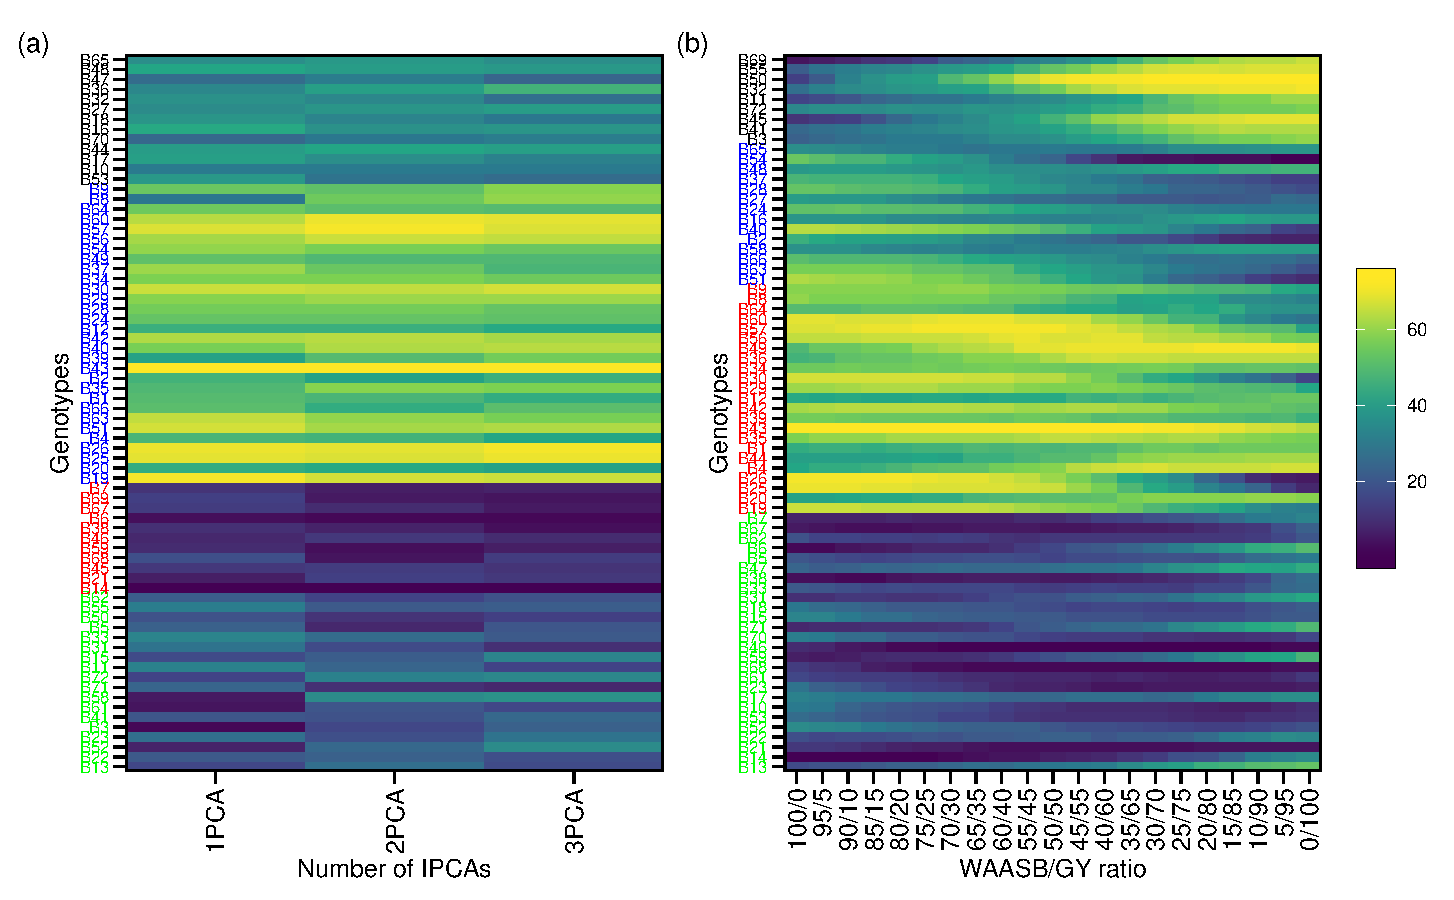
\includegraphics{figures/mod metan bb stab6-1} \end{center}

\hypertarget{coincidence-index-of-genotype-selection-1}{%
\paragraph{Coincidence index of genotype
selection}\label{coincidence-index-of-genotype-selection-1}}

Computes the coincidence index (Hamblin and Zimmermann, 1986) as
follows:

\[
{CI = \frac{A-C}{M-C}\times 100}
\]

where \emph{A} is the number of selected genotypes common to different
methods; \emph{C} is the number of expected genotypes selected by
chance; and \emph{M} is the number of genotypes selected according to
the selection intensity.

\begin{Shaded}
\begin{Highlighting}[]
\NormalTok{coinc\_1 }\OtherTok{\textless{}{-}}\NormalTok{ stab\_blups\_bb }\SpecialCharTok{\%\textgreater{}\%}\NormalTok{ dplyr}\SpecialCharTok{::}\FunctionTok{select}\NormalTok{(GEN,HMRPGV\_R) }\SpecialCharTok{\%\textgreater{}\%} \FunctionTok{arrange}\NormalTok{(HMRPGV\_R)}
\NormalTok{coinc\_2 }\OtherTok{\textless{}{-}}\NormalTok{ stab\_blups\_bb }\SpecialCharTok{\%\textgreater{}\%}\NormalTok{ dplyr}\SpecialCharTok{::}\FunctionTok{select}\NormalTok{(GEN,RPGV\_R) }\SpecialCharTok{\%\textgreater{}\%} \FunctionTok{arrange}\NormalTok{(RPGV\_R)}
\NormalTok{coinc\_3 }\OtherTok{\textless{}{-}}\NormalTok{ stab\_blups\_bb }\SpecialCharTok{\%\textgreater{}\%}\NormalTok{ dplyr}\SpecialCharTok{::}\FunctionTok{select}\NormalTok{(GEN,HMGV\_R) }\SpecialCharTok{\%\textgreater{}\%} \FunctionTok{arrange}\NormalTok{(HMGV\_R)}
\NormalTok{coinc\_4 }\OtherTok{\textless{}{-}}\NormalTok{ stab\_blups\_bb }\SpecialCharTok{\%\textgreater{}\%}\NormalTok{ dplyr}\SpecialCharTok{::}\FunctionTok{select}\NormalTok{(GEN,OrWAASBY) }\SpecialCharTok{\%\textgreater{}\%} \FunctionTok{arrange}\NormalTok{(OrWAASBY)}
\NormalTok{coinc\_5 }\OtherTok{\textless{}{-}}\NormalTok{ stab\_blups\_bb }\SpecialCharTok{\%\textgreater{}\%}\NormalTok{ dplyr}\SpecialCharTok{::}\FunctionTok{select}\NormalTok{(GEN,WAASB\_R) }\SpecialCharTok{\%\textgreater{}\%} \FunctionTok{arrange}\NormalTok{(WAASB\_R)}

\NormalTok{selc\_perc}\OtherTok{\textless{}{-}} \FunctionTok{round}\NormalTok{(}\FunctionTok{nrow}\NormalTok{(stab\_blups\_bb)}\SpecialCharTok{*}\FloatTok{0.2}\NormalTok{)}

\NormalTok{coinc\_1}\FloatTok{.1} \OtherTok{\textless{}{-}}\DecValTok{1}
\NormalTok{coinc\_1}\FloatTok{.2} \OtherTok{\textless{}{-}} \FunctionTok{coincidence\_index}\NormalTok{(}\AttributeTok{sel1 =}\NormalTok{ coinc\_1}\SpecialCharTok{$}\NormalTok{GEN[}\DecValTok{1}\SpecialCharTok{:}\NormalTok{selc\_perc], }
                                        \AttributeTok{sel2 =}\NormalTok{ coinc\_2}\SpecialCharTok{$}\NormalTok{GEN[}\DecValTok{1}\SpecialCharTok{:}\NormalTok{selc\_perc], }
                                        \AttributeTok{total =} \DecValTok{72}\NormalTok{)}\SpecialCharTok{/}\DecValTok{100}
\NormalTok{coinc\_1}\FloatTok{.3} \OtherTok{\textless{}{-}} \FunctionTok{coincidence\_index}\NormalTok{(}\AttributeTok{sel1 =}\NormalTok{ coinc\_1}\SpecialCharTok{$}\NormalTok{GEN[}\DecValTok{1}\SpecialCharTok{:}\NormalTok{selc\_perc], }
                                        \AttributeTok{sel2 =}\NormalTok{ coinc\_3}\SpecialCharTok{$}\NormalTok{GEN[}\DecValTok{1}\SpecialCharTok{:}\NormalTok{selc\_perc], }
                                        \AttributeTok{total =} \DecValTok{72}\NormalTok{)}\SpecialCharTok{/}\DecValTok{100}
\NormalTok{coinc\_1}\FloatTok{.4} \OtherTok{\textless{}{-}} \FunctionTok{coincidence\_index}\NormalTok{(}\AttributeTok{sel1 =}\NormalTok{ coinc\_1}\SpecialCharTok{$}\NormalTok{GEN[}\DecValTok{1}\SpecialCharTok{:}\NormalTok{selc\_perc], }
                                        \AttributeTok{sel2 =}\NormalTok{ coinc\_4}\SpecialCharTok{$}\NormalTok{GEN[}\DecValTok{1}\SpecialCharTok{:}\NormalTok{selc\_perc], }
                                        \AttributeTok{total =} \DecValTok{72}\NormalTok{)}\SpecialCharTok{/}\DecValTok{100}
\NormalTok{coinc\_1}\FloatTok{.5} \OtherTok{\textless{}{-}} \FunctionTok{coincidence\_index}\NormalTok{(}\AttributeTok{sel1 =}\NormalTok{ coinc\_1}\SpecialCharTok{$}\NormalTok{GEN[}\DecValTok{1}\SpecialCharTok{:}\NormalTok{selc\_perc], }
                                        \AttributeTok{sel2 =}\NormalTok{ coinc\_5}\SpecialCharTok{$}\NormalTok{GEN[}\DecValTok{1}\SpecialCharTok{:}\NormalTok{selc\_perc], }
                                        \AttributeTok{total =} \DecValTok{72}\NormalTok{)}\SpecialCharTok{/}\DecValTok{100}
\NormalTok{coinc\_2}\FloatTok{.2} \OtherTok{\textless{}{-}}\DecValTok{1}
\NormalTok{coinc\_2}\FloatTok{.3} \OtherTok{\textless{}{-}} \FunctionTok{coincidence\_index}\NormalTok{(}\AttributeTok{sel1 =}\NormalTok{ coinc\_2}\SpecialCharTok{$}\NormalTok{GEN[}\DecValTok{1}\SpecialCharTok{:}\NormalTok{selc\_perc], }
                                        \AttributeTok{sel2 =}\NormalTok{ coinc\_3}\SpecialCharTok{$}\NormalTok{GEN[}\DecValTok{1}\SpecialCharTok{:}\NormalTok{selc\_perc], }
                                        \AttributeTok{total =} \DecValTok{72}\NormalTok{)}\SpecialCharTok{/}\DecValTok{100}
\NormalTok{coinc\_2}\FloatTok{.4} \OtherTok{\textless{}{-}} \FunctionTok{coincidence\_index}\NormalTok{(}\AttributeTok{sel1 =}\NormalTok{ coinc\_2}\SpecialCharTok{$}\NormalTok{GEN[}\DecValTok{1}\SpecialCharTok{:}\NormalTok{selc\_perc], }
                                        \AttributeTok{sel2 =}\NormalTok{ coinc\_4}\SpecialCharTok{$}\NormalTok{GEN[}\DecValTok{1}\SpecialCharTok{:}\NormalTok{selc\_perc], }
                                        \AttributeTok{total =} \DecValTok{72}\NormalTok{)}\SpecialCharTok{/}\DecValTok{100}
\NormalTok{coinc\_2}\FloatTok{.5} \OtherTok{\textless{}{-}} \FunctionTok{coincidence\_index}\NormalTok{(}\AttributeTok{sel1 =}\NormalTok{ coinc\_2}\SpecialCharTok{$}\NormalTok{GEN[}\DecValTok{1}\SpecialCharTok{:}\NormalTok{selc\_perc], }
                                        \AttributeTok{sel2 =}\NormalTok{ coinc\_5}\SpecialCharTok{$}\NormalTok{GEN[}\DecValTok{1}\SpecialCharTok{:}\NormalTok{selc\_perc], }
                                        \AttributeTok{total =} \DecValTok{72}\NormalTok{)}\SpecialCharTok{/}\DecValTok{100}
\NormalTok{coinc\_3}\FloatTok{.3}\OtherTok{\textless{}{-}} \DecValTok{1}
\NormalTok{coinc\_3}\FloatTok{.4} \OtherTok{\textless{}{-}} \FunctionTok{coincidence\_index}\NormalTok{(}\AttributeTok{sel1 =}\NormalTok{ coinc\_3}\SpecialCharTok{$}\NormalTok{GEN[}\DecValTok{1}\SpecialCharTok{:}\NormalTok{selc\_perc], }
                                        \AttributeTok{sel2 =}\NormalTok{ coinc\_4}\SpecialCharTok{$}\NormalTok{GEN[}\DecValTok{1}\SpecialCharTok{:}\NormalTok{selc\_perc], }
                                        \AttributeTok{total =} \DecValTok{72}\NormalTok{)}\SpecialCharTok{/}\DecValTok{100}
\NormalTok{coinc\_3}\FloatTok{.5} \OtherTok{\textless{}{-}} \FunctionTok{coincidence\_index}\NormalTok{(}\AttributeTok{sel1 =}\NormalTok{ coinc\_3}\SpecialCharTok{$}\NormalTok{GEN[}\DecValTok{1}\SpecialCharTok{:}\NormalTok{selc\_perc], }
                                        \AttributeTok{sel2 =}\NormalTok{ coinc\_5}\SpecialCharTok{$}\NormalTok{GEN[}\DecValTok{1}\SpecialCharTok{:}\NormalTok{selc\_perc], }
                                        \AttributeTok{total =} \DecValTok{72}\NormalTok{)}\SpecialCharTok{/}\DecValTok{100}
\NormalTok{coinc\_4}\FloatTok{.4} \OtherTok{\textless{}{-}} \DecValTok{1}
\NormalTok{coinc\_4}\FloatTok{.5} \OtherTok{\textless{}{-}} \FunctionTok{coincidence\_index}\NormalTok{(}\AttributeTok{sel1 =}\NormalTok{ coinc\_4}\SpecialCharTok{$}\NormalTok{GEN[}\DecValTok{1}\SpecialCharTok{:}\NormalTok{selc\_perc], }
                                        \AttributeTok{sel2 =}\NormalTok{ coinc\_5}\SpecialCharTok{$}\NormalTok{GEN[}\DecValTok{1}\SpecialCharTok{:}\NormalTok{selc\_perc], }
                                        \AttributeTok{total =} \DecValTok{72}\NormalTok{)}\SpecialCharTok{/}\DecValTok{100}
\NormalTok{coinc\_5}\FloatTok{.5} \OtherTok{\textless{}{-}} \DecValTok{1}


\NormalTok{coinc}\OtherTok{\textless{}{-}} \FunctionTok{c}\NormalTok{(coinc\_1}\FloatTok{.1}\NormalTok{,coinc\_1}\FloatTok{.2}\NormalTok{,coinc\_2}\FloatTok{.2}\NormalTok{,coinc\_1}\FloatTok{.3}\NormalTok{,coinc\_2}\FloatTok{.3}\NormalTok{,}
\NormalTok{          coinc\_3}\FloatTok{.3}\NormalTok{,coinc\_1}\FloatTok{.4}\NormalTok{, coinc\_2}\FloatTok{.4}\NormalTok{, coinc\_3}\FloatTok{.4}\NormalTok{,}
\NormalTok{          coinc\_4}\FloatTok{.4}\NormalTok{, coinc\_1}\FloatTok{.5}\NormalTok{, coinc\_2}\FloatTok{.5}\NormalTok{,}
\NormalTok{          coinc\_3}\FloatTok{.5}\NormalTok{, coinc\_4}\FloatTok{.5}\NormalTok{,}
\NormalTok{          coinc\_5}\FloatTok{.5}\NormalTok{)}
  
\NormalTok{z}\OtherTok{=}\FunctionTok{matrix}\NormalTok{(}\DecValTok{0}\NormalTok{,}\DecValTok{5}\NormalTok{,}\DecValTok{5}\NormalTok{)}
\NormalTok{z[}\FunctionTok{upper.tri}\NormalTok{(z)}\SpecialCharTok{|} \FunctionTok{row}\NormalTok{(z)}\SpecialCharTok{==}\FunctionTok{col}\NormalTok{(z)] }\OtherTok{\textless{}{-}}\NormalTok{ coinc}

\FunctionTok{rownames}\NormalTok{(z)}\OtherTok{=}\FunctionTok{c}\NormalTok{(}
\StringTok{"HMRPGV"}\NormalTok{,}
\StringTok{"RPGV"}\NormalTok{,}
\StringTok{\textquotesingle{}HMGV\textquotesingle{}}\NormalTok{,}
\StringTok{\textquotesingle{}WAASBY\textquotesingle{}}\NormalTok{,}
\StringTok{\textquotesingle{}WAASB\textquotesingle{}}\NormalTok{)}

\FunctionTok{colnames}\NormalTok{(z)}\OtherTok{=}\FunctionTok{rownames}\NormalTok{(z)}

\NormalTok{plotBB}\OtherTok{\textless{}{-}} \FunctionTok{ggcorrplot}\NormalTok{(z, }\AttributeTok{colors =} \FunctionTok{c}\NormalTok{(}\StringTok{"\#6D9EC1"}\NormalTok{, }\StringTok{"gray"}\NormalTok{ ,}\StringTok{"\#E46726"}\NormalTok{),  }
           \AttributeTok{show.legend =}\NormalTok{ T,}
\AttributeTok{legend.title =} \StringTok{"CI"}\NormalTok{ ,}\AttributeTok{lab\_size=}\DecValTok{5}\NormalTok{,}\AttributeTok{tl.srt =} \DecValTok{90}\NormalTok{,}\AttributeTok{type =} \FunctionTok{c}\NormalTok{(}\StringTok{"upper"}\NormalTok{), }\AttributeTok{lab =}\NormalTok{ T,}\AttributeTok{digits =} \DecValTok{4}\NormalTok{,}
\AttributeTok{outline.color =} \StringTok{"white"}\NormalTok{,}\AttributeTok{pch.col =} \StringTok{"white"}\NormalTok{, }\AttributeTok{tl.col =} \StringTok{"blue"}\NormalTok{,}\AttributeTok{show.diag =}\NormalTok{ F) }\SpecialCharTok{+}
  \FunctionTok{labs}\NormalTok{(}\AttributeTok{title =} \StringTok{"BLUP{-}based stability indexes coincidence at BB"}\NormalTok{,}
           \AttributeTok{subtitle =} \StringTok{"Selection intensity of 20\% top genotypes"}\NormalTok{)}

\FunctionTok{print}\NormalTok{(plotBB)}
\end{Highlighting}
\end{Shaded}

\begin{center}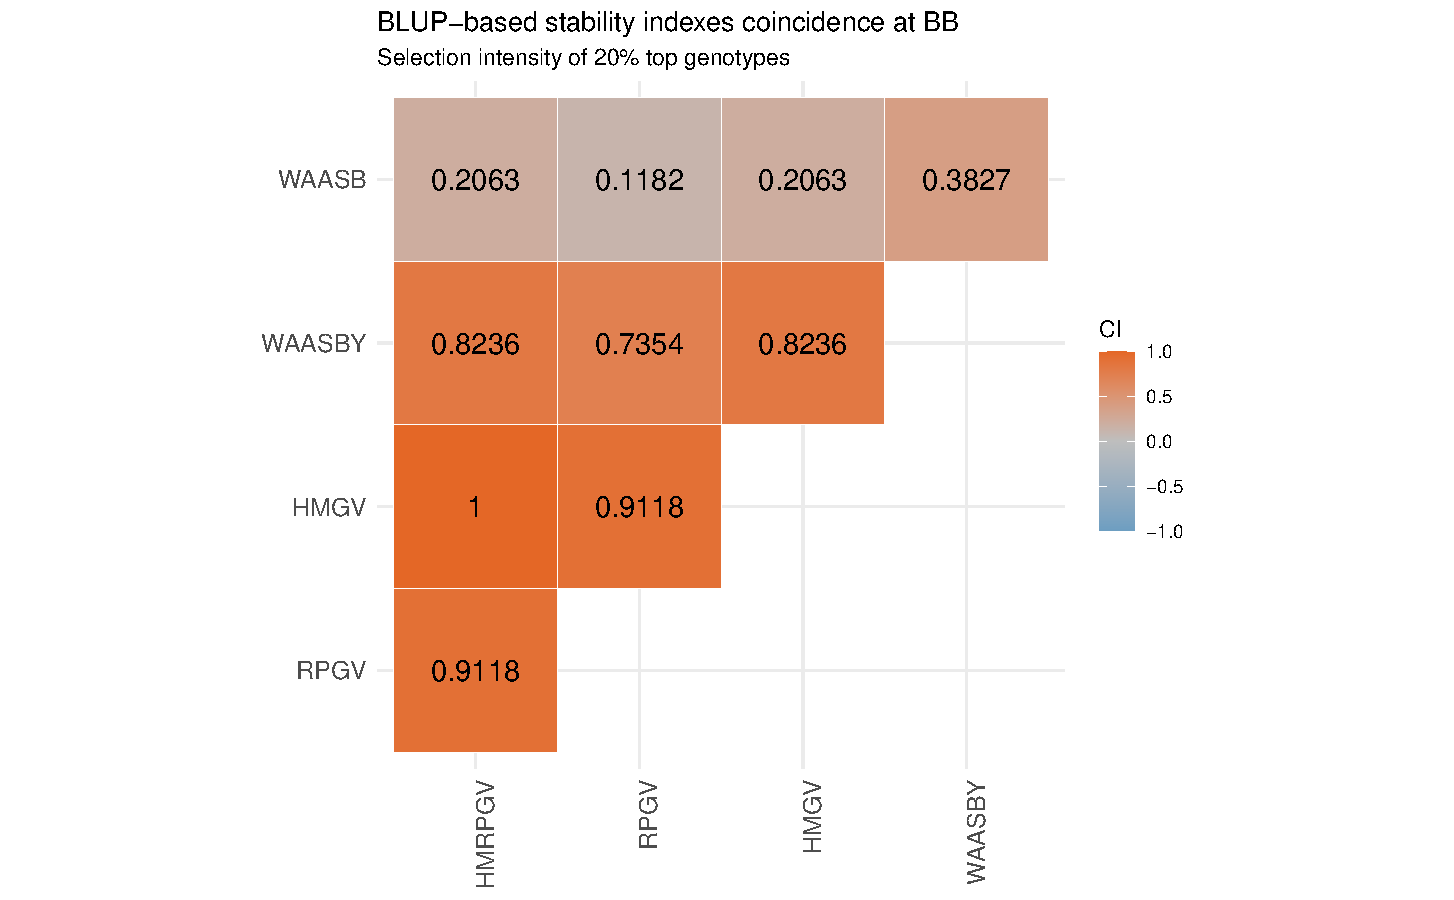
\includegraphics{figures/mod metan bb stab7-1} \end{center}

\hypertarget{met-analysis---navy-beans}{%
\subsection{\texorpdfstring{MET analysis - \textbf{Navy
beans}}{MET analysis - Navy beans}}\label{met-analysis---navy-beans}}

\hypertarget{met-analysis---asreml-2}{%
\subsubsection{MET analysis - ASReml}\label{met-analysis---asreml-2}}

Running MET using \texttt{ASReml} - only to comparison of variance
components with \texttt{metan} outputs

\begin{Shaded}
\begin{Highlighting}[]
\NormalTok{mod.met.asreml.nb1 }\OtherTok{\textless{}{-}} \FunctionTok{asreml}\NormalTok{(}\AttributeTok{fixed       =}\NormalTok{ yield }\SpecialCharTok{\textasciitilde{}}\NormalTok{  loc }\SpecialCharTok{+}\NormalTok{ loc}\SpecialCharTok{:}\NormalTok{rep,}
                     \AttributeTok{random      =} \SpecialCharTok{\textasciitilde{}}\NormalTok{  name }\SpecialCharTok{+}\NormalTok{ name}\SpecialCharTok{:}\NormalTok{loc,}
                     \AttributeTok{data        =}\NormalTok{ blues\_stage.I\_NB,}
                     \AttributeTok{predict     =} \FunctionTok{predict.asreml}\NormalTok{(}\AttributeTok{classify =} \StringTok{"name"}\NormalTok{),}
                     \AttributeTok{trace       =}\NormalTok{ F,}
                     \AttributeTok{maxit       =} \DecValTok{500}\NormalTok{)}

\NormalTok{summFix.nb.met.asreml}\OtherTok{\textless{}{-}} \FunctionTok{data.frame}\NormalTok{(}\FunctionTok{wald}\NormalTok{(mod.met.asreml.nb1))}
\NormalTok{summFix.nb.met.asreml}
\end{Highlighting}
\end{Shaded}

\global\setlength{\Oldarrayrulewidth}{\arrayrulewidth}

\global\setlength{\Oldtabcolsep}{\tabcolsep}

\setlength{\tabcolsep}{0pt}

\renewcommand*{\arraystretch}{1.5}



\providecommand{\ascline}[3]{\noalign{\global\arrayrulewidth #1}\arrayrulecolor[HTML]{#2}\cline{#3}}

\begin{longtable}[c]{|p{0.75in}|p{1.01in}|p{1.02in}|p{0.76in}}



\ascline{1.5pt}{666666}{1-4}

\multicolumn{1}{>{\raggedleft}m{\dimexpr 0.75in+0\tabcolsep}}{\textcolor[HTML]{000000}{\fontsize{9}{9}\selectfont{\global\setmainfont{Arial}{\textbf{Df}}}}} & \multicolumn{1}{>{\raggedleft}m{\dimexpr 1.01in+0\tabcolsep}}{\textcolor[HTML]{000000}{\fontsize{9}{9}\selectfont{\global\setmainfont{Arial}{\textbf{Sum.of.Sq}}}}} & \multicolumn{1}{>{\raggedleft}m{\dimexpr 1.02in+0\tabcolsep}}{\textcolor[HTML]{000000}{\fontsize{9}{9}\selectfont{\global\setmainfont{Arial}{\textbf{Wald.statistic}}}}} & \multicolumn{1}{>{\raggedleft}m{\dimexpr 0.76in+0\tabcolsep}}{\textcolor[HTML]{000000}{\fontsize{9}{9}\selectfont{\global\setmainfont{Arial}{\textbf{Pr.Chisq.}}}}} \\

\ascline{0.75pt}{666666}{1-4}



\multicolumn{1}{>{\raggedleft}m{\dimexpr 0.75in+0\tabcolsep}}{\textcolor[HTML]{999999}{\fontsize{9}{9}\selectfont{\global\setmainfont{Arial}{\textbf{numeric}}}}} & \multicolumn{1}{>{\raggedleft}m{\dimexpr 1.01in+0\tabcolsep}}{\textcolor[HTML]{999999}{\fontsize{9}{9}\selectfont{\global\setmainfont{Arial}{\textbf{numeric}}}}} & \multicolumn{1}{>{\raggedleft}m{\dimexpr 1.02in+0\tabcolsep}}{\textcolor[HTML]{999999}{\fontsize{9}{9}\selectfont{\global\setmainfont{Arial}{\textbf{numeric}}}}} & \multicolumn{1}{>{\raggedleft}m{\dimexpr 0.76in+0\tabcolsep}}{\textcolor[HTML]{999999}{\fontsize{9}{9}\selectfont{\global\setmainfont{Arial}{\textbf{numeric}}}}} \\

\ascline{1.5pt}{666666}{1-4}\endfirsthead

\ascline{1.5pt}{666666}{1-4}

\multicolumn{1}{>{\raggedleft}m{\dimexpr 0.75in+0\tabcolsep}}{\textcolor[HTML]{000000}{\fontsize{9}{9}\selectfont{\global\setmainfont{Arial}{\textbf{Df}}}}} & \multicolumn{1}{>{\raggedleft}m{\dimexpr 1.01in+0\tabcolsep}}{\textcolor[HTML]{000000}{\fontsize{9}{9}\selectfont{\global\setmainfont{Arial}{\textbf{Sum.of.Sq}}}}} & \multicolumn{1}{>{\raggedleft}m{\dimexpr 1.02in+0\tabcolsep}}{\textcolor[HTML]{000000}{\fontsize{9}{9}\selectfont{\global\setmainfont{Arial}{\textbf{Wald.statistic}}}}} & \multicolumn{1}{>{\raggedleft}m{\dimexpr 0.76in+0\tabcolsep}}{\textcolor[HTML]{000000}{\fontsize{9}{9}\selectfont{\global\setmainfont{Arial}{\textbf{Pr.Chisq.}}}}} \\

\ascline{0.75pt}{666666}{1-4}



\multicolumn{1}{>{\raggedleft}m{\dimexpr 0.75in+0\tabcolsep}}{\textcolor[HTML]{999999}{\fontsize{9}{9}\selectfont{\global\setmainfont{Arial}{\textbf{numeric}}}}} & \multicolumn{1}{>{\raggedleft}m{\dimexpr 1.01in+0\tabcolsep}}{\textcolor[HTML]{999999}{\fontsize{9}{9}\selectfont{\global\setmainfont{Arial}{\textbf{numeric}}}}} & \multicolumn{1}{>{\raggedleft}m{\dimexpr 1.02in+0\tabcolsep}}{\textcolor[HTML]{999999}{\fontsize{9}{9}\selectfont{\global\setmainfont{Arial}{\textbf{numeric}}}}} & \multicolumn{1}{>{\raggedleft}m{\dimexpr 0.76in+0\tabcolsep}}{\textcolor[HTML]{999999}{\fontsize{9}{9}\selectfont{\global\setmainfont{Arial}{\textbf{numeric}}}}} \\

\ascline{1.5pt}{666666}{1-4}\endhead



\multicolumn{4}{>{\raggedleft}m{\dimexpr 3.54in+6\tabcolsep}}{\textcolor[HTML]{000000}{\fontsize{9}{9}\selectfont{\global\setmainfont{Arial}{n:\ 4}}}} \\

\ascline{0.75pt}{666666}{1-4}\endfoot



\multicolumn{1}{>{\raggedleft}m{\dimexpr 0.75in+0\tabcolsep}}{\textcolor[HTML]{000000}{\fontsize{9}{9}\selectfont{\global\setmainfont{Arial}{1}}}} & \multicolumn{1}{>{\raggedleft}m{\dimexpr 1.01in+0\tabcolsep}}{\textcolor[HTML]{000000}{\fontsize{9}{9}\selectfont{\global\setmainfont{Arial}{1,636,916,005}}}} & \multicolumn{1}{>{\raggedleft}m{\dimexpr 1.02in+0\tabcolsep}}{\textcolor[HTML]{000000}{\fontsize{9}{9}\selectfont{\global\setmainfont{Arial}{9,420.3}}}} & \multicolumn{1}{>{\raggedleft}m{\dimexpr 0.76in+0\tabcolsep}}{\textcolor[HTML]{000000}{\fontsize{9}{9}\selectfont{\global\setmainfont{Arial}{0}}}} \\

\ascline{0.75pt}{666666}{1-4}



\multicolumn{1}{>{\raggedleft}m{\dimexpr 0.75in+0\tabcolsep}}{\textcolor[HTML]{000000}{\fontsize{9}{9}\selectfont{\global\setmainfont{Arial}{3}}}} & \multicolumn{1}{>{\raggedleft}m{\dimexpr 1.01in+0\tabcolsep}}{\textcolor[HTML]{000000}{\fontsize{9}{9}\selectfont{\global\setmainfont{Arial}{11,631,057}}}} & \multicolumn{1}{>{\raggedleft}m{\dimexpr 1.02in+0\tabcolsep}}{\textcolor[HTML]{000000}{\fontsize{9}{9}\selectfont{\global\setmainfont{Arial}{66.9}}}} & \multicolumn{1}{>{\raggedleft}m{\dimexpr 0.76in+0\tabcolsep}}{\textcolor[HTML]{000000}{\fontsize{9}{9}\selectfont{\global\setmainfont{Arial}{0}}}} \\

\ascline{0.75pt}{666666}{1-4}



\multicolumn{1}{>{\raggedleft}m{\dimexpr 0.75in+0\tabcolsep}}{\textcolor[HTML]{000000}{\fontsize{9}{9}\selectfont{\global\setmainfont{Arial}{12}}}} & \multicolumn{1}{>{\raggedleft}m{\dimexpr 1.01in+0\tabcolsep}}{\textcolor[HTML]{000000}{\fontsize{9}{9}\selectfont{\global\setmainfont{Arial}{20,821,488}}}} & \multicolumn{1}{>{\raggedleft}m{\dimexpr 1.02in+0\tabcolsep}}{\textcolor[HTML]{000000}{\fontsize{9}{9}\selectfont{\global\setmainfont{Arial}{119.8}}}} & \multicolumn{1}{>{\raggedleft}m{\dimexpr 0.76in+0\tabcolsep}}{\textcolor[HTML]{000000}{\fontsize{9}{9}\selectfont{\global\setmainfont{Arial}{0}}}} \\

\ascline{0.75pt}{666666}{1-4}



\multicolumn{1}{>{\raggedleft}m{\dimexpr 0.75in+0\tabcolsep}}{\textcolor[HTML]{000000}{\fontsize{9}{9}\selectfont{\global\setmainfont{Arial}{}}}} & \multicolumn{1}{>{\raggedleft}m{\dimexpr 1.01in+0\tabcolsep}}{\textcolor[HTML]{000000}{\fontsize{9}{9}\selectfont{\global\setmainfont{Arial}{173,765}}}} & \multicolumn{1}{>{\raggedleft}m{\dimexpr 1.02in+0\tabcolsep}}{\textcolor[HTML]{000000}{\fontsize{9}{9}\selectfont{\global\setmainfont{Arial}{}}}} & \multicolumn{1}{>{\raggedleft}m{\dimexpr 0.76in+0\tabcolsep}}{\textcolor[HTML]{000000}{\fontsize{9}{9}\selectfont{\global\setmainfont{Arial}{}}}} \\

\ascline{1.5pt}{666666}{1-4}



\end{longtable}



\arrayrulecolor[HTML]{000000}

\global\setlength{\arrayrulewidth}{\Oldarrayrulewidth}

\global\setlength{\tabcolsep}{\Oldtabcolsep}

\renewcommand*{\arraystretch}{1}

\begin{Shaded}
\begin{Highlighting}[]
\NormalTok{summ.nb.met.asreml}\OtherTok{\textless{}{-}} \FunctionTok{data.frame}\NormalTok{(}\FunctionTok{summary.asreml}\NormalTok{(mod.met.asreml.nb1)}\SpecialCharTok{$}\NormalTok{varcomp)}
\NormalTok{summ.nb.met.asreml}
\end{Highlighting}
\end{Shaded}

\global\setlength{\Oldarrayrulewidth}{\arrayrulewidth}

\global\setlength{\Oldtabcolsep}{\tabcolsep}

\setlength{\tabcolsep}{0pt}

\renewcommand*{\arraystretch}{1.5}



\providecommand{\ascline}[3]{\noalign{\global\arrayrulewidth #1}\arrayrulecolor[HTML]{#2}\cline{#3}}

\begin{longtable}[c]{|p{0.88in}|p{0.75in}|p{0.75in}|p{0.77in}|p{0.75in}}



\ascline{1.5pt}{666666}{1-5}

\multicolumn{1}{>{\raggedleft}m{\dimexpr 0.88in+0\tabcolsep}}{\textcolor[HTML]{000000}{\fontsize{9}{9}\selectfont{\global\setmainfont{Arial}{\textbf{component}}}}} & \multicolumn{1}{>{\raggedleft}m{\dimexpr 0.75in+0\tabcolsep}}{\textcolor[HTML]{000000}{\fontsize{9}{9}\selectfont{\global\setmainfont{Arial}{\textbf{std.error}}}}} & \multicolumn{1}{>{\raggedleft}m{\dimexpr 0.75in+0\tabcolsep}}{\textcolor[HTML]{000000}{\fontsize{9}{9}\selectfont{\global\setmainfont{Arial}{\textbf{z.ratio}}}}} & \multicolumn{1}{>{\raggedright}m{\dimexpr 0.77in+0\tabcolsep}}{\textcolor[HTML]{000000}{\fontsize{9}{9}\selectfont{\global\setmainfont{Arial}{\textbf{bound}}}}} & \multicolumn{1}{>{\raggedleft}m{\dimexpr 0.75in+0\tabcolsep}}{\textcolor[HTML]{000000}{\fontsize{9}{9}\selectfont{\global\setmainfont{Arial}{\textbf{X.ch}}}}} \\

\ascline{0.75pt}{666666}{1-5}



\multicolumn{1}{>{\raggedleft}m{\dimexpr 0.88in+0\tabcolsep}}{\textcolor[HTML]{999999}{\fontsize{9}{9}\selectfont{\global\setmainfont{Arial}{\textbf{numeric}}}}} & \multicolumn{1}{>{\raggedleft}m{\dimexpr 0.75in+0\tabcolsep}}{\textcolor[HTML]{999999}{\fontsize{9}{9}\selectfont{\global\setmainfont{Arial}{\textbf{numeric}}}}} & \multicolumn{1}{>{\raggedleft}m{\dimexpr 0.75in+0\tabcolsep}}{\textcolor[HTML]{999999}{\fontsize{9}{9}\selectfont{\global\setmainfont{Arial}{\textbf{numeric}}}}} & \multicolumn{1}{>{\raggedright}m{\dimexpr 0.77in+0\tabcolsep}}{\textcolor[HTML]{999999}{\fontsize{9}{9}\selectfont{\global\setmainfont{Arial}{\textbf{character}}}}} & \multicolumn{1}{>{\raggedleft}m{\dimexpr 0.75in+0\tabcolsep}}{\textcolor[HTML]{999999}{\fontsize{9}{9}\selectfont{\global\setmainfont{Arial}{\textbf{numeric}}}}} \\

\ascline{1.5pt}{666666}{1-5}\endfirsthead

\ascline{1.5pt}{666666}{1-5}

\multicolumn{1}{>{\raggedleft}m{\dimexpr 0.88in+0\tabcolsep}}{\textcolor[HTML]{000000}{\fontsize{9}{9}\selectfont{\global\setmainfont{Arial}{\textbf{component}}}}} & \multicolumn{1}{>{\raggedleft}m{\dimexpr 0.75in+0\tabcolsep}}{\textcolor[HTML]{000000}{\fontsize{9}{9}\selectfont{\global\setmainfont{Arial}{\textbf{std.error}}}}} & \multicolumn{1}{>{\raggedleft}m{\dimexpr 0.75in+0\tabcolsep}}{\textcolor[HTML]{000000}{\fontsize{9}{9}\selectfont{\global\setmainfont{Arial}{\textbf{z.ratio}}}}} & \multicolumn{1}{>{\raggedright}m{\dimexpr 0.77in+0\tabcolsep}}{\textcolor[HTML]{000000}{\fontsize{9}{9}\selectfont{\global\setmainfont{Arial}{\textbf{bound}}}}} & \multicolumn{1}{>{\raggedleft}m{\dimexpr 0.75in+0\tabcolsep}}{\textcolor[HTML]{000000}{\fontsize{9}{9}\selectfont{\global\setmainfont{Arial}{\textbf{X.ch}}}}} \\

\ascline{0.75pt}{666666}{1-5}



\multicolumn{1}{>{\raggedleft}m{\dimexpr 0.88in+0\tabcolsep}}{\textcolor[HTML]{999999}{\fontsize{9}{9}\selectfont{\global\setmainfont{Arial}{\textbf{numeric}}}}} & \multicolumn{1}{>{\raggedleft}m{\dimexpr 0.75in+0\tabcolsep}}{\textcolor[HTML]{999999}{\fontsize{9}{9}\selectfont{\global\setmainfont{Arial}{\textbf{numeric}}}}} & \multicolumn{1}{>{\raggedleft}m{\dimexpr 0.75in+0\tabcolsep}}{\textcolor[HTML]{999999}{\fontsize{9}{9}\selectfont{\global\setmainfont{Arial}{\textbf{numeric}}}}} & \multicolumn{1}{>{\raggedright}m{\dimexpr 0.77in+0\tabcolsep}}{\textcolor[HTML]{999999}{\fontsize{9}{9}\selectfont{\global\setmainfont{Arial}{\textbf{character}}}}} & \multicolumn{1}{>{\raggedleft}m{\dimexpr 0.75in+0\tabcolsep}}{\textcolor[HTML]{999999}{\fontsize{9}{9}\selectfont{\global\setmainfont{Arial}{\textbf{numeric}}}}} \\

\ascline{1.5pt}{666666}{1-5}\endhead



\multicolumn{5}{>{\raggedleft}m{\dimexpr 3.91in+8\tabcolsep}}{\textcolor[HTML]{000000}{\fontsize{9}{9}\selectfont{\global\setmainfont{Arial}{n:\ 3}}}} \\

\ascline{0.75pt}{666666}{1-5}\endfoot



\multicolumn{1}{>{\raggedleft}m{\dimexpr 0.88in+0\tabcolsep}}{\textcolor[HTML]{000000}{\fontsize{9}{9}\selectfont{\global\setmainfont{Arial}{34,501.8}}}} & \multicolumn{1}{>{\raggedleft}m{\dimexpr 0.75in+0\tabcolsep}}{\textcolor[HTML]{000000}{\fontsize{9}{9}\selectfont{\global\setmainfont{Arial}{11,258.8}}}} & \multicolumn{1}{>{\raggedleft}m{\dimexpr 0.75in+0\tabcolsep}}{\textcolor[HTML]{000000}{\fontsize{9}{9}\selectfont{\global\setmainfont{Arial}{3.1}}}} & \multicolumn{1}{>{\raggedright}m{\dimexpr 0.77in+0\tabcolsep}}{\textcolor[HTML]{000000}{\fontsize{9}{9}\selectfont{\global\setmainfont{Arial}{P}}}} & \multicolumn{1}{>{\raggedleft}m{\dimexpr 0.75in+0\tabcolsep}}{\textcolor[HTML]{000000}{\fontsize{9}{9}\selectfont{\global\setmainfont{Arial}{0}}}} \\

\ascline{0.75pt}{666666}{1-5}



\multicolumn{1}{>{\raggedleft}m{\dimexpr 0.88in+0\tabcolsep}}{\textcolor[HTML]{000000}{\fontsize{9}{9}\selectfont{\global\setmainfont{Arial}{72,760.9}}}} & \multicolumn{1}{>{\raggedleft}m{\dimexpr 0.75in+0\tabcolsep}}{\textcolor[HTML]{000000}{\fontsize{9}{9}\selectfont{\global\setmainfont{Arial}{11,918.4}}}} & \multicolumn{1}{>{\raggedleft}m{\dimexpr 0.75in+0\tabcolsep}}{\textcolor[HTML]{000000}{\fontsize{9}{9}\selectfont{\global\setmainfont{Arial}{6.1}}}} & \multicolumn{1}{>{\raggedright}m{\dimexpr 0.77in+0\tabcolsep}}{\textcolor[HTML]{000000}{\fontsize{9}{9}\selectfont{\global\setmainfont{Arial}{P}}}} & \multicolumn{1}{>{\raggedleft}m{\dimexpr 0.75in+0\tabcolsep}}{\textcolor[HTML]{000000}{\fontsize{9}{9}\selectfont{\global\setmainfont{Arial}{0}}}} \\

\ascline{0.75pt}{666666}{1-5}



\multicolumn{1}{>{\raggedleft}m{\dimexpr 0.88in+0\tabcolsep}}{\textcolor[HTML]{000000}{\fontsize{9}{9}\selectfont{\global\setmainfont{Arial}{173,765.2}}}} & \multicolumn{1}{>{\raggedleft}m{\dimexpr 0.75in+0\tabcolsep}}{\textcolor[HTML]{000000}{\fontsize{9}{9}\selectfont{\global\setmainfont{Arial}{8,797.2}}}} & \multicolumn{1}{>{\raggedleft}m{\dimexpr 0.75in+0\tabcolsep}}{\textcolor[HTML]{000000}{\fontsize{9}{9}\selectfont{\global\setmainfont{Arial}{19.8}}}} & \multicolumn{1}{>{\raggedright}m{\dimexpr 0.77in+0\tabcolsep}}{\textcolor[HTML]{000000}{\fontsize{9}{9}\selectfont{\global\setmainfont{Arial}{P}}}} & \multicolumn{1}{>{\raggedleft}m{\dimexpr 0.75in+0\tabcolsep}}{\textcolor[HTML]{000000}{\fontsize{9}{9}\selectfont{\global\setmainfont{Arial}{0}}}} \\

\ascline{1.5pt}{666666}{1-5}



\end{longtable}



\arrayrulecolor[HTML]{000000}

\global\setlength{\arrayrulewidth}{\Oldarrayrulewidth}

\global\setlength{\tabcolsep}{\Oldtabcolsep}

\renewcommand*{\arraystretch}{1}

\begin{Shaded}
\begin{Highlighting}[]
\CommentTok{\#print(summary.asreml(mod.met.asreml.nb1)$bic)}
\NormalTok{mod.met.asreml.nb}\OtherTok{\textless{}{-}} \FunctionTok{as.data.frame}\NormalTok{((mod.met.asreml.nb1}\SpecialCharTok{$}\NormalTok{predictions}\SpecialCharTok{$}\NormalTok{pvals[}\DecValTok{1}\SpecialCharTok{:}\DecValTok{3}\NormalTok{]))}
\FunctionTok{names}\NormalTok{(mod.met.asreml.nb) }\OtherTok{\textless{}{-}} \FunctionTok{c}\NormalTok{(}\StringTok{"name"}\NormalTok{, }\StringTok{"yield\_BLUPS\_MET"}\NormalTok{, }\StringTok{"SE"}\NormalTok{)}

\DocumentationTok{\#\#\#}
\end{Highlighting}
\end{Shaded}

\hypertarget{met-analysis---lme4-2}{%
\subsubsection{MET analysis - lme4}\label{met-analysis---lme4-2}}

Running MET using \texttt{metan} R package
\href{Olivoto\%20et\%20al.,\%202019a}{@olivotoMeanPerformanceStability2019}.

\begin{Shaded}
\begin{Highlighting}[]
\CommentTok{\#str(blues\_stage.I\_NB)}
\NormalTok{mixed\_mod.nb}\OtherTok{\textless{}{-}} 
   \FunctionTok{gamem\_met}\NormalTok{(blues\_stage.I\_NB,}
             \AttributeTok{env =}\NormalTok{ loc,}
             \AttributeTok{gen =}\NormalTok{ name,}
             \AttributeTok{rep =}\NormalTok{ rep,}
             \AttributeTok{resp =}\NormalTok{ yield,}
             \AttributeTok{random =} \StringTok{"gen"}\NormalTok{, }\CommentTok{\#Default}
             \AttributeTok{verbose =} \ConstantTok{TRUE}\NormalTok{) }\CommentTok{\#Default}
\end{Highlighting}
\end{Shaded}

Evaluating trait yield
\textbar=================================================================================================================================================================================================\textbar{}
100\% 00:00:03

\begin{verbatim}
#> Method: REML/BLUP
\end{verbatim}

\begin{verbatim}
#> Random effects: GEN, GEN:ENV
\end{verbatim}

\begin{verbatim}
#> Fixed effects: ENV, REP(ENV)
\end{verbatim}

\begin{verbatim}
#> Denominador DF: Satterthwaite's method
\end{verbatim}

\begin{longtable}[]{@{}
  >{\raggedright\arraybackslash}p{(\columnwidth - 0\tabcolsep) * \real{1.0000}}@{}}
\toprule\noalign{}
\begin{minipage}[b]{\linewidth}\raggedright
P-values for Likelihood Ratio Test of the analyzed traits
\end{minipage} \\
\midrule\noalign{}
\endhead
\bottomrule\noalign{}
\endlastfoot
model yield COMPLETE NA GEN 3.41e-05 GEN:ENV 6.69e-20 \\
\end{longtable}

All variables with significant (p \textless{} 0.05)
genotype-vs-environment interaction

\hypertarget{printing-the-model-outputs-2}{%
\subsubsection{Printing the model
outputs}\label{printing-the-model-outputs-2}}

\hypertarget{likelihood-ratio-tests-2}{%
\paragraph{Likelihood Ratio Tests}\label{likelihood-ratio-tests-2}}

The output \texttt{LRT} contains the Likelihood Ratio Tests for genotype
and genotype-vs-environment random effects.

\begin{Shaded}
\begin{Highlighting}[]
\NormalTok{data\_mod\_nb\_test }\OtherTok{\textless{}{-}} \FunctionTok{get\_model\_data}\NormalTok{(mixed\_mod.nb, }\StringTok{"lrt"}\NormalTok{)}
\end{Highlighting}
\end{Shaded}

\begin{verbatim}
#> Class of the model: waasb
\end{verbatim}

\begin{verbatim}
#> Variable extracted: lrt
\end{verbatim}

\begin{Shaded}
\begin{Highlighting}[]
\NormalTok{data\_mod\_nb\_test}
\end{Highlighting}
\end{Shaded}

\global\setlength{\Oldarrayrulewidth}{\arrayrulewidth}

\global\setlength{\Oldtabcolsep}{\tabcolsep}

\setlength{\tabcolsep}{0pt}

\renewcommand*{\arraystretch}{1.5}



\providecommand{\ascline}[3]{\noalign{\global\arrayrulewidth #1}\arrayrulecolor[HTML]{#2}\cline{#3}}

\begin{longtable}[c]{|p{0.77in}|p{0.77in}|p{0.75in}|p{0.75in}|p{0.75in}|p{0.75in}|p{0.75in}|p{0.85in}}



\ascline{1.5pt}{666666}{1-8}

\multicolumn{1}{>{\raggedright}m{\dimexpr 0.77in+0\tabcolsep}}{\textcolor[HTML]{000000}{\fontsize{9}{9}\selectfont{\global\setmainfont{Arial}{\textbf{VAR}}}}} & \multicolumn{1}{>{\raggedright}m{\dimexpr 0.77in+0\tabcolsep}}{\textcolor[HTML]{000000}{\fontsize{9}{9}\selectfont{\global\setmainfont{Arial}{\textbf{model}}}}} & \multicolumn{1}{>{\raggedleft}m{\dimexpr 0.75in+0\tabcolsep}}{\textcolor[HTML]{000000}{\fontsize{9}{9}\selectfont{\global\setmainfont{Arial}{\textbf{npar}}}}} & \multicolumn{1}{>{\raggedleft}m{\dimexpr 0.75in+0\tabcolsep}}{\textcolor[HTML]{000000}{\fontsize{9}{9}\selectfont{\global\setmainfont{Arial}{\textbf{logLik}}}}} & \multicolumn{1}{>{\raggedleft}m{\dimexpr 0.75in+0\tabcolsep}}{\textcolor[HTML]{000000}{\fontsize{9}{9}\selectfont{\global\setmainfont{Arial}{\textbf{AIC}}}}} & \multicolumn{1}{>{\raggedleft}m{\dimexpr 0.75in+0\tabcolsep}}{\textcolor[HTML]{000000}{\fontsize{9}{9}\selectfont{\global\setmainfont{Arial}{\textbf{LRT}}}}} & \multicolumn{1}{>{\raggedleft}m{\dimexpr 0.75in+0\tabcolsep}}{\textcolor[HTML]{000000}{\fontsize{9}{9}\selectfont{\global\setmainfont{Arial}{\textbf{Df}}}}} & \multicolumn{1}{>{\raggedleft}m{\dimexpr 0.85in+0\tabcolsep}}{\textcolor[HTML]{000000}{\fontsize{9}{9}\selectfont{\global\setmainfont{Arial}{\textbf{Pr(>Chisq)}}}}} \\

\ascline{0.75pt}{666666}{1-8}



\multicolumn{1}{>{\raggedright}m{\dimexpr 0.77in+0\tabcolsep}}{\textcolor[HTML]{999999}{\fontsize{9}{9}\selectfont{\global\setmainfont{Arial}{\textbf{character}}}}} & \multicolumn{1}{>{\raggedright}m{\dimexpr 0.77in+0\tabcolsep}}{\textcolor[HTML]{999999}{\fontsize{9}{9}\selectfont{\global\setmainfont{Arial}{\textbf{character}}}}} & \multicolumn{1}{>{\raggedleft}m{\dimexpr 0.75in+0\tabcolsep}}{\textcolor[HTML]{999999}{\fontsize{9}{9}\selectfont{\global\setmainfont{Arial}{\textbf{integer}}}}} & \multicolumn{1}{>{\raggedleft}m{\dimexpr 0.75in+0\tabcolsep}}{\textcolor[HTML]{999999}{\fontsize{9}{9}\selectfont{\global\setmainfont{Arial}{\textbf{numeric}}}}} & \multicolumn{1}{>{\raggedleft}m{\dimexpr 0.75in+0\tabcolsep}}{\textcolor[HTML]{999999}{\fontsize{9}{9}\selectfont{\global\setmainfont{Arial}{\textbf{numeric}}}}} & \multicolumn{1}{>{\raggedleft}m{\dimexpr 0.75in+0\tabcolsep}}{\textcolor[HTML]{999999}{\fontsize{9}{9}\selectfont{\global\setmainfont{Arial}{\textbf{numeric}}}}} & \multicolumn{1}{>{\raggedleft}m{\dimexpr 0.75in+0\tabcolsep}}{\textcolor[HTML]{999999}{\fontsize{9}{9}\selectfont{\global\setmainfont{Arial}{\textbf{numeric}}}}} & \multicolumn{1}{>{\raggedleft}m{\dimexpr 0.85in+0\tabcolsep}}{\textcolor[HTML]{999999}{\fontsize{9}{9}\selectfont{\global\setmainfont{Arial}{\textbf{numeric}}}}} \\

\ascline{1.5pt}{666666}{1-8}\endfirsthead

\ascline{1.5pt}{666666}{1-8}

\multicolumn{1}{>{\raggedright}m{\dimexpr 0.77in+0\tabcolsep}}{\textcolor[HTML]{000000}{\fontsize{9}{9}\selectfont{\global\setmainfont{Arial}{\textbf{VAR}}}}} & \multicolumn{1}{>{\raggedright}m{\dimexpr 0.77in+0\tabcolsep}}{\textcolor[HTML]{000000}{\fontsize{9}{9}\selectfont{\global\setmainfont{Arial}{\textbf{model}}}}} & \multicolumn{1}{>{\raggedleft}m{\dimexpr 0.75in+0\tabcolsep}}{\textcolor[HTML]{000000}{\fontsize{9}{9}\selectfont{\global\setmainfont{Arial}{\textbf{npar}}}}} & \multicolumn{1}{>{\raggedleft}m{\dimexpr 0.75in+0\tabcolsep}}{\textcolor[HTML]{000000}{\fontsize{9}{9}\selectfont{\global\setmainfont{Arial}{\textbf{logLik}}}}} & \multicolumn{1}{>{\raggedleft}m{\dimexpr 0.75in+0\tabcolsep}}{\textcolor[HTML]{000000}{\fontsize{9}{9}\selectfont{\global\setmainfont{Arial}{\textbf{AIC}}}}} & \multicolumn{1}{>{\raggedleft}m{\dimexpr 0.75in+0\tabcolsep}}{\textcolor[HTML]{000000}{\fontsize{9}{9}\selectfont{\global\setmainfont{Arial}{\textbf{LRT}}}}} & \multicolumn{1}{>{\raggedleft}m{\dimexpr 0.75in+0\tabcolsep}}{\textcolor[HTML]{000000}{\fontsize{9}{9}\selectfont{\global\setmainfont{Arial}{\textbf{Df}}}}} & \multicolumn{1}{>{\raggedleft}m{\dimexpr 0.85in+0\tabcolsep}}{\textcolor[HTML]{000000}{\fontsize{9}{9}\selectfont{\global\setmainfont{Arial}{\textbf{Pr(>Chisq)}}}}} \\

\ascline{0.75pt}{666666}{1-8}



\multicolumn{1}{>{\raggedright}m{\dimexpr 0.77in+0\tabcolsep}}{\textcolor[HTML]{999999}{\fontsize{9}{9}\selectfont{\global\setmainfont{Arial}{\textbf{character}}}}} & \multicolumn{1}{>{\raggedright}m{\dimexpr 0.77in+0\tabcolsep}}{\textcolor[HTML]{999999}{\fontsize{9}{9}\selectfont{\global\setmainfont{Arial}{\textbf{character}}}}} & \multicolumn{1}{>{\raggedleft}m{\dimexpr 0.75in+0\tabcolsep}}{\textcolor[HTML]{999999}{\fontsize{9}{9}\selectfont{\global\setmainfont{Arial}{\textbf{integer}}}}} & \multicolumn{1}{>{\raggedleft}m{\dimexpr 0.75in+0\tabcolsep}}{\textcolor[HTML]{999999}{\fontsize{9}{9}\selectfont{\global\setmainfont{Arial}{\textbf{numeric}}}}} & \multicolumn{1}{>{\raggedleft}m{\dimexpr 0.75in+0\tabcolsep}}{\textcolor[HTML]{999999}{\fontsize{9}{9}\selectfont{\global\setmainfont{Arial}{\textbf{numeric}}}}} & \multicolumn{1}{>{\raggedleft}m{\dimexpr 0.75in+0\tabcolsep}}{\textcolor[HTML]{999999}{\fontsize{9}{9}\selectfont{\global\setmainfont{Arial}{\textbf{numeric}}}}} & \multicolumn{1}{>{\raggedleft}m{\dimexpr 0.75in+0\tabcolsep}}{\textcolor[HTML]{999999}{\fontsize{9}{9}\selectfont{\global\setmainfont{Arial}{\textbf{numeric}}}}} & \multicolumn{1}{>{\raggedleft}m{\dimexpr 0.85in+0\tabcolsep}}{\textcolor[HTML]{999999}{\fontsize{9}{9}\selectfont{\global\setmainfont{Arial}{\textbf{numeric}}}}} \\

\ascline{1.5pt}{666666}{1-8}\endhead



\multicolumn{8}{>{\raggedright}m{\dimexpr 6.14in+14\tabcolsep}}{\textcolor[HTML]{000000}{\fontsize{9}{9}\selectfont{\global\setmainfont{Arial}{n:\ 2}}}} \\

\ascline{0.75pt}{666666}{1-8}\endfoot



\multicolumn{1}{>{\raggedright}m{\dimexpr 0.77in+0\tabcolsep}}{\textcolor[HTML]{000000}{\fontsize{9}{9}\selectfont{\global\setmainfont{Arial}{yield}}}} & \multicolumn{1}{>{\raggedright}m{\dimexpr 0.77in+0\tabcolsep}}{\textcolor[HTML]{000000}{\fontsize{9}{9}\selectfont{\global\setmainfont{Arial}{GEN}}}} & \multicolumn{1}{>{\raggedleft}m{\dimexpr 0.75in+0\tabcolsep}}{\textcolor[HTML]{000000}{\fontsize{9}{9}\selectfont{\global\setmainfont{Arial}{18}}}} & \multicolumn{1}{>{\raggedleft}m{\dimexpr 0.75in+0\tabcolsep}}{\textcolor[HTML]{000000}{\fontsize{9}{9}\selectfont{\global\setmainfont{Arial}{-8,123.2}}}} & \multicolumn{1}{>{\raggedleft}m{\dimexpr 0.75in+0\tabcolsep}}{\textcolor[HTML]{000000}{\fontsize{9}{9}\selectfont{\global\setmainfont{Arial}{16,282.4}}}} & \multicolumn{1}{>{\raggedleft}m{\dimexpr 0.75in+0\tabcolsep}}{\textcolor[HTML]{000000}{\fontsize{9}{9}\selectfont{\global\setmainfont{Arial}{17.2}}}} & \multicolumn{1}{>{\raggedleft}m{\dimexpr 0.75in+0\tabcolsep}}{\textcolor[HTML]{000000}{\fontsize{9}{9}\selectfont{\global\setmainfont{Arial}{1}}}} & \multicolumn{1}{>{\raggedleft}m{\dimexpr 0.85in+0\tabcolsep}}{\textcolor[HTML]{000000}{\fontsize{9}{9}\selectfont{\global\setmainfont{Arial}{0.0}}}} \\

\ascline{0.75pt}{666666}{1-8}



\multicolumn{1}{>{\raggedright}m{\dimexpr 0.77in+0\tabcolsep}}{\textcolor[HTML]{000000}{\fontsize{9}{9}\selectfont{\global\setmainfont{Arial}{yield}}}} & \multicolumn{1}{>{\raggedright}m{\dimexpr 0.77in+0\tabcolsep}}{\textcolor[HTML]{000000}{\fontsize{9}{9}\selectfont{\global\setmainfont{Arial}{GEN:ENV}}}} & \multicolumn{1}{>{\raggedleft}m{\dimexpr 0.75in+0\tabcolsep}}{\textcolor[HTML]{000000}{\fontsize{9}{9}\selectfont{\global\setmainfont{Arial}{18}}}} & \multicolumn{1}{>{\raggedleft}m{\dimexpr 0.75in+0\tabcolsep}}{\textcolor[HTML]{000000}{\fontsize{9}{9}\selectfont{\global\setmainfont{Arial}{-8,156.3}}}} & \multicolumn{1}{>{\raggedleft}m{\dimexpr 0.75in+0\tabcolsep}}{\textcolor[HTML]{000000}{\fontsize{9}{9}\selectfont{\global\setmainfont{Arial}{16,348.7}}}} & \multicolumn{1}{>{\raggedleft}m{\dimexpr 0.75in+0\tabcolsep}}{\textcolor[HTML]{000000}{\fontsize{9}{9}\selectfont{\global\setmainfont{Arial}{83.4}}}} & \multicolumn{1}{>{\raggedleft}m{\dimexpr 0.75in+0\tabcolsep}}{\textcolor[HTML]{000000}{\fontsize{9}{9}\selectfont{\global\setmainfont{Arial}{1}}}} & \multicolumn{1}{>{\raggedleft}m{\dimexpr 0.85in+0\tabcolsep}}{\textcolor[HTML]{000000}{\fontsize{9}{9}\selectfont{\global\setmainfont{Arial}{0.0}}}} \\

\ascline{1.5pt}{666666}{1-8}



\end{longtable}



\arrayrulecolor[HTML]{000000}

\global\setlength{\arrayrulewidth}{\Oldarrayrulewidth}

\global\setlength{\tabcolsep}{\Oldtabcolsep}

\renewcommand*{\arraystretch}{1}

\begin{Shaded}
\begin{Highlighting}[]
\CommentTok{\#customize the display of numbers and other data in a tibble}
\CommentTok{\# old \textless{}{-} options(pillar.sigfig = 6)}
\CommentTok{\# }
\CommentTok{\# blues\_stage.I\_NB \%\textgreater{}\%}
\CommentTok{\#   group\_by(loc) \%\textgreater{}\%}
\CommentTok{\#   dplyr::summarise(Mean = mean(yield, na.rm = TRUE))}
\end{Highlighting}
\end{Shaded}

\hypertarget{detailed-parameters-2}{%
\paragraph{Detailed parameters}\label{detailed-parameters-2}}

\begin{Shaded}
\begin{Highlighting}[]
\NormalTok{data\_mod\_nb\_det }\OtherTok{\textless{}{-}} \FunctionTok{get\_model\_data}\NormalTok{(mixed\_mod.nb, }\StringTok{"details"}\NormalTok{)}
\end{Highlighting}
\end{Shaded}

\begin{verbatim}
#> Class of the model: waasb
\end{verbatim}

\begin{verbatim}
#> Variable extracted: details
\end{verbatim}

\begin{Shaded}
\begin{Highlighting}[]
\NormalTok{data\_mod\_nb\_det}
\end{Highlighting}
\end{Shaded}

\global\setlength{\Oldarrayrulewidth}{\arrayrulewidth}

\global\setlength{\Oldtabcolsep}{\tabcolsep}

\setlength{\tabcolsep}{0pt}

\renewcommand*{\arraystretch}{1.5}



\providecommand{\ascline}[3]{\noalign{\global\arrayrulewidth #1}\arrayrulecolor[HTML]{#2}\cline{#3}}

\begin{longtable}[c]{|p{0.89in}|p{1.34in}}



\ascline{1.5pt}{666666}{1-2}

\multicolumn{1}{>{\raggedright}m{\dimexpr 0.89in+0\tabcolsep}}{\textcolor[HTML]{000000}{\fontsize{9}{9}\selectfont{\global\setmainfont{Arial}{\textbf{Parameters}}}}} & \multicolumn{1}{>{\raggedright}m{\dimexpr 1.34in+0\tabcolsep}}{\textcolor[HTML]{000000}{\fontsize{9}{9}\selectfont{\global\setmainfont{Arial}{\textbf{yield}}}}} \\

\ascline{0.75pt}{666666}{1-2}



\multicolumn{1}{>{\raggedright}m{\dimexpr 0.89in+0\tabcolsep}}{\textcolor[HTML]{999999}{\fontsize{9}{9}\selectfont{\global\setmainfont{Arial}{\textbf{character}}}}} & \multicolumn{1}{>{\raggedright}m{\dimexpr 1.34in+0\tabcolsep}}{\textcolor[HTML]{999999}{\fontsize{9}{9}\selectfont{\global\setmainfont{Arial}{\textbf{character}}}}} \\

\ascline{1.5pt}{666666}{1-2}\endfirsthead

\ascline{1.5pt}{666666}{1-2}

\multicolumn{1}{>{\raggedright}m{\dimexpr 0.89in+0\tabcolsep}}{\textcolor[HTML]{000000}{\fontsize{9}{9}\selectfont{\global\setmainfont{Arial}{\textbf{Parameters}}}}} & \multicolumn{1}{>{\raggedright}m{\dimexpr 1.34in+0\tabcolsep}}{\textcolor[HTML]{000000}{\fontsize{9}{9}\selectfont{\global\setmainfont{Arial}{\textbf{yield}}}}} \\

\ascline{0.75pt}{666666}{1-2}



\multicolumn{1}{>{\raggedright}m{\dimexpr 0.89in+0\tabcolsep}}{\textcolor[HTML]{999999}{\fontsize{9}{9}\selectfont{\global\setmainfont{Arial}{\textbf{character}}}}} & \multicolumn{1}{>{\raggedright}m{\dimexpr 1.34in+0\tabcolsep}}{\textcolor[HTML]{999999}{\fontsize{9}{9}\selectfont{\global\setmainfont{Arial}{\textbf{character}}}}} \\

\ascline{1.5pt}{666666}{1-2}\endhead



\multicolumn{2}{>{\raggedright}m{\dimexpr 2.24in+2\tabcolsep}}{\textcolor[HTML]{000000}{\fontsize{9}{9}\selectfont{\global\setmainfont{Arial}{n:\ 12}}}} \\

\ascline{0.75pt}{666666}{1-2}\endfoot



\multicolumn{1}{>{\raggedright}m{\dimexpr 0.89in+0\tabcolsep}}{\textcolor[HTML]{000000}{\fontsize{9}{9}\selectfont{\global\setmainfont{Arial}{Mean}}}} & \multicolumn{1}{>{\raggedright}m{\dimexpr 1.34in+0\tabcolsep}}{\textcolor[HTML]{000000}{\fontsize{9}{9}\selectfont{\global\setmainfont{Arial}{2924}}}} \\

\ascline{0.75pt}{666666}{1-2}



\multicolumn{1}{>{\raggedright}m{\dimexpr 0.89in+0\tabcolsep}}{\textcolor[HTML]{000000}{\fontsize{9}{9}\selectfont{\global\setmainfont{Arial}{SE}}}} & \multicolumn{1}{>{\raggedright}m{\dimexpr 1.34in+0\tabcolsep}}{\textcolor[HTML]{000000}{\fontsize{9}{9}\selectfont{\global\setmainfont{Arial}{17.22}}}} \\

\ascline{0.75pt}{666666}{1-2}



\multicolumn{1}{>{\raggedright}m{\dimexpr 0.89in+0\tabcolsep}}{\textcolor[HTML]{000000}{\fontsize{9}{9}\selectfont{\global\setmainfont{Arial}{SD}}}} & \multicolumn{1}{>{\raggedright}m{\dimexpr 1.34in+0\tabcolsep}}{\textcolor[HTML]{000000}{\fontsize{9}{9}\selectfont{\global\setmainfont{Arial}{565.35}}}} \\

\ascline{0.75pt}{666666}{1-2}



\multicolumn{1}{>{\raggedright}m{\dimexpr 0.89in+0\tabcolsep}}{\textcolor[HTML]{000000}{\fontsize{9}{9}\selectfont{\global\setmainfont{Arial}{CV}}}} & \multicolumn{1}{>{\raggedright}m{\dimexpr 1.34in+0\tabcolsep}}{\textcolor[HTML]{000000}{\fontsize{9}{9}\selectfont{\global\setmainfont{Arial}{19.34}}}} \\

\ascline{0.75pt}{666666}{1-2}



\multicolumn{1}{>{\raggedright}m{\dimexpr 0.89in+0\tabcolsep}}{\textcolor[HTML]{000000}{\fontsize{9}{9}\selectfont{\global\setmainfont{Arial}{Min}}}} & \multicolumn{1}{>{\raggedright}m{\dimexpr 1.34in+0\tabcolsep}}{\textcolor[HTML]{000000}{\fontsize{9}{9}\selectfont{\global\setmainfont{Arial}{1096.13\ (N32\ in\ BA)}}}} \\

\ascline{0.75pt}{666666}{1-2}



\multicolumn{1}{>{\raggedright}m{\dimexpr 0.89in+0\tabcolsep}}{\textcolor[HTML]{000000}{\fontsize{9}{9}\selectfont{\global\setmainfont{Arial}{Max}}}} & \multicolumn{1}{>{\raggedright}m{\dimexpr 1.34in+0\tabcolsep}}{\textcolor[HTML]{000000}{\fontsize{9}{9}\selectfont{\global\setmainfont{Arial}{4939.4\ (N34\ in\ TU)}}}} \\

\ascline{0.75pt}{666666}{1-2}



\multicolumn{1}{>{\raggedright}m{\dimexpr 0.89in+0\tabcolsep}}{\textcolor[HTML]{000000}{\fontsize{9}{9}\selectfont{\global\setmainfont{Arial}{MinENV}}}} & \multicolumn{1}{>{\raggedright}m{\dimexpr 1.34in+0\tabcolsep}}{\textcolor[HTML]{000000}{\fontsize{9}{9}\selectfont{\global\setmainfont{Arial}{BA\ (2654.03)}}}} \\

\ascline{0.75pt}{666666}{1-2}



\multicolumn{1}{>{\raggedright}m{\dimexpr 0.89in+0\tabcolsep}}{\textcolor[HTML]{000000}{\fontsize{9}{9}\selectfont{\global\setmainfont{Arial}{MaxENV}}}} & \multicolumn{1}{>{\raggedright}m{\dimexpr 1.34in+0\tabcolsep}}{\textcolor[HTML]{000000}{\fontsize{9}{9}\selectfont{\global\setmainfont{Arial}{HU\ (3094)}}}} \\

\ascline{0.75pt}{666666}{1-2}



\multicolumn{1}{>{\raggedright}m{\dimexpr 0.89in+0\tabcolsep}}{\textcolor[HTML]{000000}{\fontsize{9}{9}\selectfont{\global\setmainfont{Arial}{MinGEN}}}} & \multicolumn{1}{>{\raggedright}m{\dimexpr 1.34in+0\tabcolsep}}{\textcolor[HTML]{000000}{\fontsize{9}{9}\selectfont{\global\setmainfont{Arial}{N28\ (2260.58)\ }}}} \\

\ascline{1.5pt}{666666}{1-2}



\end{longtable}



\arrayrulecolor[HTML]{000000}

\global\setlength{\arrayrulewidth}{\Oldarrayrulewidth}

\global\setlength{\tabcolsep}{\Oldtabcolsep}

\renewcommand*{\arraystretch}{1}

\hypertarget{random-effects-2}{%
\paragraph{Random effects}\label{random-effects-2}}

The output \texttt{LRT} contains the Likelihood Ratio Tests for genotype
and genotype-vs-environment random effects.

\begin{Shaded}
\begin{Highlighting}[]
\NormalTok{old }\OtherTok{\textless{}{-}} \FunctionTok{options}\NormalTok{(}\AttributeTok{pillar.sigfig =} \DecValTok{8}\NormalTok{)}

\NormalTok{data\_mod\_nb\_var }\OtherTok{\textless{}{-}} \FunctionTok{get\_model\_data}\NormalTok{(mixed\_mod.nb, }\StringTok{"vcomp"}\NormalTok{)}
\end{Highlighting}
\end{Shaded}

\begin{verbatim}
#> Class of the model: waasb
\end{verbatim}

\begin{verbatim}
#> Variable extracted: vcomp
\end{verbatim}

\begin{Shaded}
\begin{Highlighting}[]
\NormalTok{data\_mod\_nb\_var}
\end{Highlighting}
\end{Shaded}

\global\setlength{\Oldarrayrulewidth}{\arrayrulewidth}

\global\setlength{\Oldtabcolsep}{\tabcolsep}

\setlength{\tabcolsep}{0pt}

\renewcommand*{\arraystretch}{1.5}



\providecommand{\ascline}[3]{\noalign{\global\arrayrulewidth #1}\arrayrulecolor[HTML]{#2}\cline{#3}}

\begin{longtable}[c]{|p{0.77in}|p{0.77in}}



\ascline{1.5pt}{666666}{1-2}

\multicolumn{1}{>{\raggedright}m{\dimexpr 0.77in+0\tabcolsep}}{\textcolor[HTML]{000000}{\fontsize{9}{9}\selectfont{\global\setmainfont{Arial}{\textbf{Group}}}}} & \multicolumn{1}{>{\raggedleft}m{\dimexpr 0.77in+0\tabcolsep}}{\textcolor[HTML]{000000}{\fontsize{9}{9}\selectfont{\global\setmainfont{Arial}{\textbf{yield}}}}} \\

\ascline{0.75pt}{666666}{1-2}



\multicolumn{1}{>{\raggedright}m{\dimexpr 0.77in+0\tabcolsep}}{\textcolor[HTML]{999999}{\fontsize{9}{9}\selectfont{\global\setmainfont{Arial}{\textbf{character}}}}} & \multicolumn{1}{>{\raggedleft}m{\dimexpr 0.77in+0\tabcolsep}}{\textcolor[HTML]{999999}{\fontsize{9}{9}\selectfont{\global\setmainfont{Arial}{\textbf{numeric}}}}} \\

\ascline{1.5pt}{666666}{1-2}\endfirsthead

\ascline{1.5pt}{666666}{1-2}

\multicolumn{1}{>{\raggedright}m{\dimexpr 0.77in+0\tabcolsep}}{\textcolor[HTML]{000000}{\fontsize{9}{9}\selectfont{\global\setmainfont{Arial}{\textbf{Group}}}}} & \multicolumn{1}{>{\raggedleft}m{\dimexpr 0.77in+0\tabcolsep}}{\textcolor[HTML]{000000}{\fontsize{9}{9}\selectfont{\global\setmainfont{Arial}{\textbf{yield}}}}} \\

\ascline{0.75pt}{666666}{1-2}



\multicolumn{1}{>{\raggedright}m{\dimexpr 0.77in+0\tabcolsep}}{\textcolor[HTML]{999999}{\fontsize{9}{9}\selectfont{\global\setmainfont{Arial}{\textbf{character}}}}} & \multicolumn{1}{>{\raggedleft}m{\dimexpr 0.77in+0\tabcolsep}}{\textcolor[HTML]{999999}{\fontsize{9}{9}\selectfont{\global\setmainfont{Arial}{\textbf{numeric}}}}} \\

\ascline{1.5pt}{666666}{1-2}\endhead



\multicolumn{2}{>{\raggedright}m{\dimexpr 1.54in+2\tabcolsep}}{\textcolor[HTML]{000000}{\fontsize{9}{9}\selectfont{\global\setmainfont{Arial}{n:\ 3}}}} \\

\ascline{0.75pt}{666666}{1-2}\endfoot



\multicolumn{1}{>{\raggedright}m{\dimexpr 0.77in+0\tabcolsep}}{\textcolor[HTML]{000000}{\fontsize{9}{9}\selectfont{\global\setmainfont{Arial}{GEN}}}} & \multicolumn{1}{>{\raggedleft}m{\dimexpr 0.77in+0\tabcolsep}}{\textcolor[HTML]{000000}{\fontsize{9}{9}\selectfont{\global\setmainfont{Arial}{34,502.1}}}} \\

\ascline{0.75pt}{666666}{1-2}



\multicolumn{1}{>{\raggedright}m{\dimexpr 0.77in+0\tabcolsep}}{\textcolor[HTML]{000000}{\fontsize{9}{9}\selectfont{\global\setmainfont{Arial}{GEN:ENV}}}} & \multicolumn{1}{>{\raggedleft}m{\dimexpr 0.77in+0\tabcolsep}}{\textcolor[HTML]{000000}{\fontsize{9}{9}\selectfont{\global\setmainfont{Arial}{72,760.9}}}} \\

\ascline{0.75pt}{666666}{1-2}



\multicolumn{1}{>{\raggedright}m{\dimexpr 0.77in+0\tabcolsep}}{\textcolor[HTML]{000000}{\fontsize{9}{9}\selectfont{\global\setmainfont{Arial}{Residual}}}} & \multicolumn{1}{>{\raggedleft}m{\dimexpr 0.77in+0\tabcolsep}}{\textcolor[HTML]{000000}{\fontsize{9}{9}\selectfont{\global\setmainfont{Arial}{173,765.0}}}} \\

\ascline{1.5pt}{666666}{1-2}



\end{longtable}



\arrayrulecolor[HTML]{000000}

\global\setlength{\arrayrulewidth}{\Oldarrayrulewidth}

\global\setlength{\tabcolsep}{\Oldtabcolsep}

\renewcommand*{\arraystretch}{1}

\hypertarget{variance-components-and-genetic-parameters-2}{%
\paragraph{Variance components and genetic
parameters}\label{variance-components-and-genetic-parameters-2}}

\begin{Shaded}
\begin{Highlighting}[]
\NormalTok{old }\OtherTok{\textless{}{-}} \FunctionTok{options}\NormalTok{(}\AttributeTok{pillar.sigfig =} \DecValTok{4}\NormalTok{)}

\NormalTok{data\_mod\_nb\_comp }\OtherTok{\textless{}{-}} \FunctionTok{get\_model\_data}\NormalTok{(mixed\_mod.nb)}
\end{Highlighting}
\end{Shaded}

\begin{verbatim}
#> Class of the model: waasb
\end{verbatim}

\begin{verbatim}
#> Variable extracted: genpar
\end{verbatim}

\begin{Shaded}
\begin{Highlighting}[]
\NormalTok{data\_mod\_nb\_comp}
\end{Highlighting}
\end{Shaded}

\global\setlength{\Oldarrayrulewidth}{\arrayrulewidth}

\global\setlength{\Oldtabcolsep}{\tabcolsep}

\setlength{\tabcolsep}{0pt}

\renewcommand*{\arraystretch}{1.5}



\providecommand{\ascline}[3]{\noalign{\global\arrayrulewidth #1}\arrayrulecolor[HTML]{#2}\cline{#3}}

\begin{longtable}[c]{|p{1.34in}|p{0.77in}}



\ascline{1.5pt}{666666}{1-2}

\multicolumn{1}{>{\raggedright}m{\dimexpr 1.34in+0\tabcolsep}}{\textcolor[HTML]{000000}{\fontsize{9}{9}\selectfont{\global\setmainfont{Arial}{\textbf{Parameters}}}}} & \multicolumn{1}{>{\raggedleft}m{\dimexpr 0.77in+0\tabcolsep}}{\textcolor[HTML]{000000}{\fontsize{9}{9}\selectfont{\global\setmainfont{Arial}{\textbf{yield}}}}} \\

\ascline{0.75pt}{666666}{1-2}



\multicolumn{1}{>{\raggedright}m{\dimexpr 1.34in+0\tabcolsep}}{\textcolor[HTML]{999999}{\fontsize{9}{9}\selectfont{\global\setmainfont{Arial}{\textbf{character}}}}} & \multicolumn{1}{>{\raggedleft}m{\dimexpr 0.77in+0\tabcolsep}}{\textcolor[HTML]{999999}{\fontsize{9}{9}\selectfont{\global\setmainfont{Arial}{\textbf{numeric}}}}} \\

\ascline{1.5pt}{666666}{1-2}\endfirsthead

\ascline{1.5pt}{666666}{1-2}

\multicolumn{1}{>{\raggedright}m{\dimexpr 1.34in+0\tabcolsep}}{\textcolor[HTML]{000000}{\fontsize{9}{9}\selectfont{\global\setmainfont{Arial}{\textbf{Parameters}}}}} & \multicolumn{1}{>{\raggedleft}m{\dimexpr 0.77in+0\tabcolsep}}{\textcolor[HTML]{000000}{\fontsize{9}{9}\selectfont{\global\setmainfont{Arial}{\textbf{yield}}}}} \\

\ascline{0.75pt}{666666}{1-2}



\multicolumn{1}{>{\raggedright}m{\dimexpr 1.34in+0\tabcolsep}}{\textcolor[HTML]{999999}{\fontsize{9}{9}\selectfont{\global\setmainfont{Arial}{\textbf{character}}}}} & \multicolumn{1}{>{\raggedleft}m{\dimexpr 0.77in+0\tabcolsep}}{\textcolor[HTML]{999999}{\fontsize{9}{9}\selectfont{\global\setmainfont{Arial}{\textbf{numeric}}}}} \\

\ascline{1.5pt}{666666}{1-2}\endhead



\multicolumn{2}{>{\raggedright}m{\dimexpr 2.1in+2\tabcolsep}}{\textcolor[HTML]{000000}{\fontsize{9}{9}\selectfont{\global\setmainfont{Arial}{n:\ 9}}}} \\

\ascline{0.75pt}{666666}{1-2}\endfoot



\multicolumn{1}{>{\raggedright}m{\dimexpr 1.34in+0\tabcolsep}}{\textcolor[HTML]{000000}{\fontsize{9}{9}\selectfont{\global\setmainfont{Arial}{Phenotypic\ variance}}}} & \multicolumn{1}{>{\raggedleft}m{\dimexpr 0.77in+0\tabcolsep}}{\textcolor[HTML]{000000}{\fontsize{9}{9}\selectfont{\global\setmainfont{Arial}{281,028.0}}}} \\

\ascline{0.75pt}{666666}{1-2}



\multicolumn{1}{>{\raggedright}m{\dimexpr 1.34in+0\tabcolsep}}{\textcolor[HTML]{000000}{\fontsize{9}{9}\selectfont{\global\setmainfont{Arial}{Heritability}}}} & \multicolumn{1}{>{\raggedleft}m{\dimexpr 0.77in+0\tabcolsep}}{\textcolor[HTML]{000000}{\fontsize{9}{9}\selectfont{\global\setmainfont{Arial}{0.1}}}} \\

\ascline{0.75pt}{666666}{1-2}



\multicolumn{1}{>{\raggedright}m{\dimexpr 1.34in+0\tabcolsep}}{\textcolor[HTML]{000000}{\fontsize{9}{9}\selectfont{\global\setmainfont{Arial}{GEIr2}}}} & \multicolumn{1}{>{\raggedleft}m{\dimexpr 0.77in+0\tabcolsep}}{\textcolor[HTML]{000000}{\fontsize{9}{9}\selectfont{\global\setmainfont{Arial}{0.3}}}} \\

\ascline{0.75pt}{666666}{1-2}



\multicolumn{1}{>{\raggedright}m{\dimexpr 1.34in+0\tabcolsep}}{\textcolor[HTML]{000000}{\fontsize{9}{9}\selectfont{\global\setmainfont{Arial}{h2mg}}}} & \multicolumn{1}{>{\raggedleft}m{\dimexpr 0.77in+0\tabcolsep}}{\textcolor[HTML]{000000}{\fontsize{9}{9}\selectfont{\global\setmainfont{Arial}{0.5}}}} \\

\ascline{0.75pt}{666666}{1-2}



\multicolumn{1}{>{\raggedright}m{\dimexpr 1.34in+0\tabcolsep}}{\textcolor[HTML]{000000}{\fontsize{9}{9}\selectfont{\global\setmainfont{Arial}{Accuracy}}}} & \multicolumn{1}{>{\raggedleft}m{\dimexpr 0.77in+0\tabcolsep}}{\textcolor[HTML]{000000}{\fontsize{9}{9}\selectfont{\global\setmainfont{Arial}{0.7}}}} \\

\ascline{0.75pt}{666666}{1-2}



\multicolumn{1}{>{\raggedright}m{\dimexpr 1.34in+0\tabcolsep}}{\textcolor[HTML]{000000}{\fontsize{9}{9}\selectfont{\global\setmainfont{Arial}{rge}}}} & \multicolumn{1}{>{\raggedleft}m{\dimexpr 0.77in+0\tabcolsep}}{\textcolor[HTML]{000000}{\fontsize{9}{9}\selectfont{\global\setmainfont{Arial}{0.3}}}} \\

\ascline{0.75pt}{666666}{1-2}



\multicolumn{1}{>{\raggedright}m{\dimexpr 1.34in+0\tabcolsep}}{\textcolor[HTML]{000000}{\fontsize{9}{9}\selectfont{\global\setmainfont{Arial}{CVg}}}} & \multicolumn{1}{>{\raggedleft}m{\dimexpr 0.77in+0\tabcolsep}}{\textcolor[HTML]{000000}{\fontsize{9}{9}\selectfont{\global\setmainfont{Arial}{6.4}}}} \\

\ascline{0.75pt}{666666}{1-2}



\multicolumn{1}{>{\raggedright}m{\dimexpr 1.34in+0\tabcolsep}}{\textcolor[HTML]{000000}{\fontsize{9}{9}\selectfont{\global\setmainfont{Arial}{CVr}}}} & \multicolumn{1}{>{\raggedleft}m{\dimexpr 0.77in+0\tabcolsep}}{\textcolor[HTML]{000000}{\fontsize{9}{9}\selectfont{\global\setmainfont{Arial}{14.3}}}} \\

\ascline{0.75pt}{666666}{1-2}



\multicolumn{1}{>{\raggedright}m{\dimexpr 1.34in+0\tabcolsep}}{\textcolor[HTML]{000000}{\fontsize{9}{9}\selectfont{\global\setmainfont{Arial}{CV\ ratio}}}} & \multicolumn{1}{>{\raggedleft}m{\dimexpr 0.77in+0\tabcolsep}}{\textcolor[HTML]{000000}{\fontsize{9}{9}\selectfont{\global\setmainfont{Arial}{0.4}}}} \\

\ascline{1.5pt}{666666}{1-2}



\end{longtable}



\arrayrulecolor[HTML]{000000}

\global\setlength{\arrayrulewidth}{\Oldarrayrulewidth}

\global\setlength{\tabcolsep}{\Oldtabcolsep}

\renewcommand*{\arraystretch}{1}

\hypertarget{met---gge-biplot-2}{%
\subsubsection{MET - GGE biplot}\label{met---gge-biplot-2}}

Genotype plus Genotype-vs-Environment interaction (GGE).
Mega-environment identification in multi-environment trials (MET)
according to \href{link\%20here}{@W. Yan et al.~2007}

\hypertarget{gge-env-biplot-2}{%
\paragraph{GGE ENV biplot}\label{gge-env-biplot-2}}

GGE biplot done using:

\begin{itemize}
\tightlist
\item
  \textbf{sd}: each value is divided by the standard deviation of its
  corresponding environment.
\item
  \textbf{environment}: environment-centered (G+GE)
\item
  \textbf{environment}: singular value is entirely partitioned into the
  environment eigenvectors, also called column metric preserving
\end{itemize}

\begin{Shaded}
\begin{Highlighting}[]
\NormalTok{gge\_model.nb }\OtherTok{\textless{}{-}} \FunctionTok{gge}\NormalTok{(blues\_stage.I\_NB, loc, name, yield, }
                    \AttributeTok{centering =} \StringTok{"environment"}\NormalTok{, }\CommentTok{\#1}
                    \AttributeTok{scaling =} \StringTok{"sd"}\NormalTok{, }\CommentTok{\#2}
                    \AttributeTok{svp =} \StringTok{"environment"}\NormalTok{)}\CommentTok{\#2}

\NormalTok{a }\OtherTok{\textless{}{-}} \FunctionTok{plot}\NormalTok{(gge\_model.nb, }\AttributeTok{type=}\DecValTok{4}\NormalTok{,}
          \AttributeTok{size.text.env =} \FloatTok{4.5}\NormalTok{,}
          \AttributeTok{plot\_theme =} \FunctionTok{theme\_metan}\NormalTok{(}\AttributeTok{grid =}  \StringTok{"both"}\NormalTok{,}\AttributeTok{color.background =} \FunctionTok{transparent\_color}\NormalTok{()),}
         \AttributeTok{axis\_expand =} \FloatTok{1.5}\NormalTok{,}
         \AttributeTok{col.alpha.circle =} \FloatTok{0.8}\NormalTok{,}
         \AttributeTok{shape.gen =} \ConstantTok{NA}\NormalTok{,}
         \AttributeTok{col.gen =} \ConstantTok{NA}\NormalTok{,}
         \AttributeTok{size.text.lab =} \ConstantTok{NA}\NormalTok{,}
         \AttributeTok{size.text.gen =} \ConstantTok{NA}\NormalTok{,}
         \AttributeTok{leg.lab=}\FunctionTok{c}\NormalTok{(}\StringTok{\textquotesingle{}Env\textquotesingle{}}\NormalTok{)}
         \CommentTok{\#title = FALSE}
\NormalTok{         )}


\NormalTok{gge\_model.nb }\OtherTok{\textless{}{-}} \FunctionTok{gge}\NormalTok{(blues\_stage.I\_NB, loc, name, yield,}
                    \AttributeTok{centering =} \StringTok{"environment"}\NormalTok{, }\CommentTok{\#1}
                    \AttributeTok{scaling =} \StringTok{"sd"}\NormalTok{, }\CommentTok{\#2Y}
                    \AttributeTok{svp =} \StringTok{"environment"}\NormalTok{)}\CommentTok{\#2)}

\NormalTok{b }\OtherTok{\textless{}{-}} \FunctionTok{plot}\NormalTok{(gge\_model.nb, }\AttributeTok{type =} \DecValTok{6}\NormalTok{,}
             \AttributeTok{size.text.env =} \DecValTok{5}\NormalTok{,}
          \AttributeTok{plot\_theme =} \FunctionTok{theme\_metan}\NormalTok{(}\AttributeTok{grid =}  \StringTok{"both"}\NormalTok{,}\AttributeTok{color.background =} \FunctionTok{transparent\_color}\NormalTok{()),}
         \AttributeTok{axis\_expand =} \FloatTok{1.5}\NormalTok{,}
        \CommentTok{\# col.alpha.circle = 100,}
          \AttributeTok{col.alpha.circle =} \FloatTok{0.8}\NormalTok{,}
         \AttributeTok{size.text.lab =} \DecValTok{13}
        \CommentTok{\#title = FALSE}
\NormalTok{        )}

 \FunctionTok{arrange\_ggplot}\NormalTok{(a, b,}
                \AttributeTok{guides =} \StringTok{"collect"}\NormalTok{,}
  \AttributeTok{tag\_levels =} \StringTok{"a"}\NormalTok{,}
  \AttributeTok{tag\_prefix =} \StringTok{"("}\NormalTok{,}
  \AttributeTok{tag\_suffix =} \StringTok{")"}\NormalTok{)}
\end{Highlighting}
\end{Shaded}

\begin{center}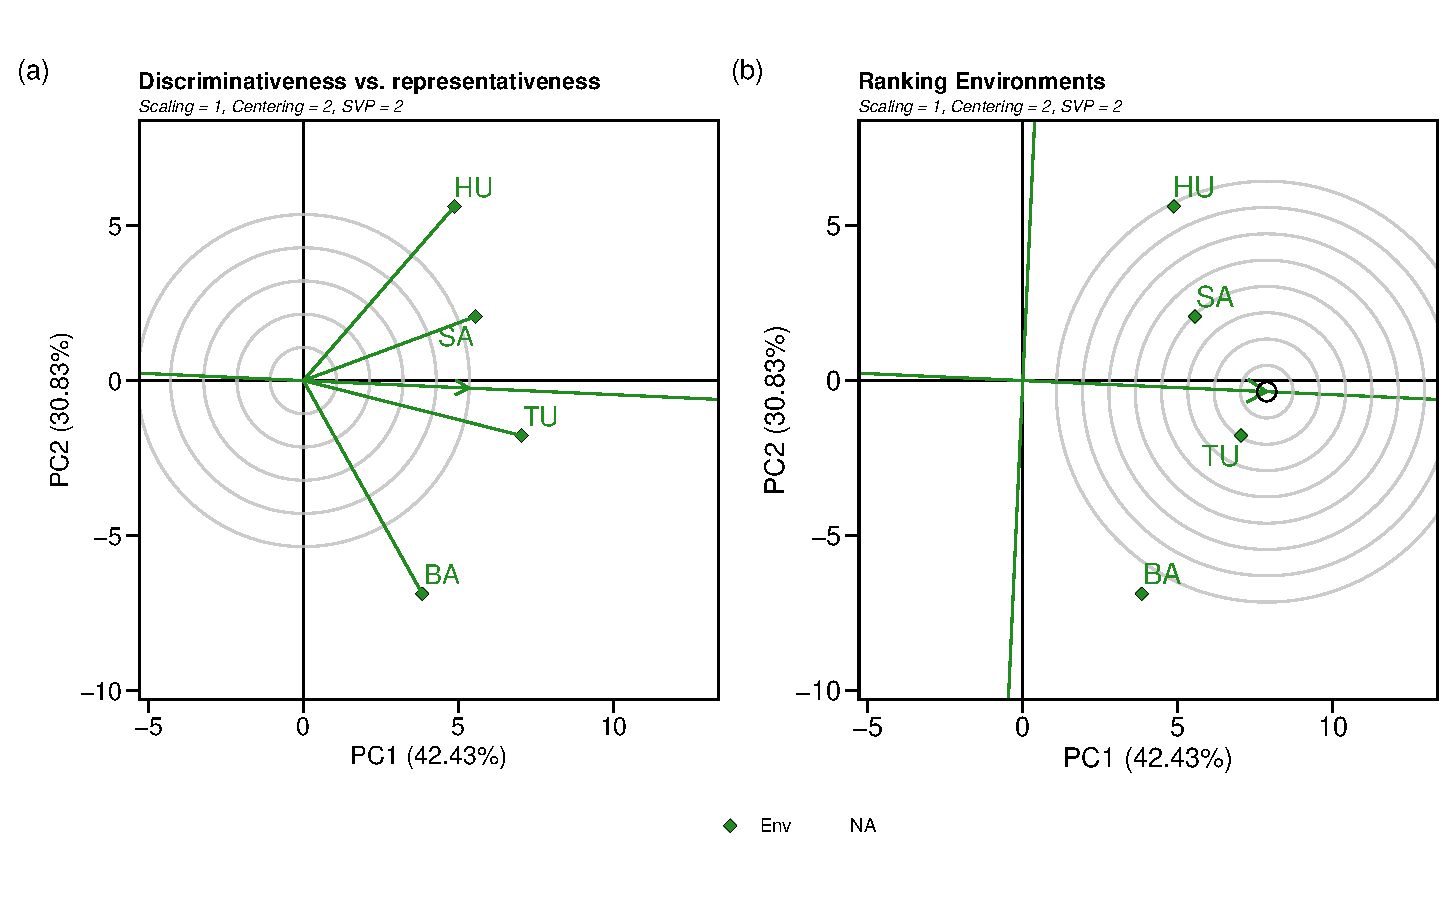
\includegraphics{figures/nb gge fig1-1} \end{center}

\hypertarget{biplot-type-3-which-won-where-2}{%
\paragraph{Biplot type 3:
Which-won-where}\label{biplot-type-3-which-won-where-2}}

GGE biplot done using:

\begin{itemize}
\tightlist
\item
  \textbf{sd}: each value is divided by the standard deviation of its
  corresponding environment.
\item
  \textbf{environment}: environment-centered (G+GE)
\item
  \textbf{genotype}: singular value is entirely partitioned into the
  environment eigenvectors, also called column metric preserving
\end{itemize}

\begin{Shaded}
\begin{Highlighting}[]
\NormalTok{gge\_model.nb }\OtherTok{\textless{}{-}} \FunctionTok{gge}\NormalTok{(blues\_stage.I\_NB, loc, name, yield,}
                     \AttributeTok{centering =} \StringTok{"environment"}\NormalTok{, }\CommentTok{\#2}
                    \AttributeTok{scaling =} \StringTok{"sd"}\NormalTok{, }\CommentTok{\#1}
                    \AttributeTok{svp =} \StringTok{"genotype"}\NormalTok{)}\CommentTok{\#2)}

\NormalTok{e }\OtherTok{\textless{}{-}} \FunctionTok{plot}\NormalTok{(gge\_model.nb, }\AttributeTok{type =} \DecValTok{3}\NormalTok{,}
          \AttributeTok{size.text.env =} \DecValTok{5}\NormalTok{,}
          \AttributeTok{plot\_theme =} \FunctionTok{theme\_metan}\NormalTok{(}\AttributeTok{grid =}  \StringTok{"both"}\NormalTok{,}\AttributeTok{color.background =} \FunctionTok{transparent\_color}\NormalTok{()),}
         \AttributeTok{axis\_expand =} \FloatTok{1.2}\NormalTok{,}
         \AttributeTok{size.line =} \FloatTok{0.7}\NormalTok{,}
         \AttributeTok{size.text.gen =} \DecValTok{4}\NormalTok{,}
         \AttributeTok{size.text.win =} \FloatTok{4.5}
         \CommentTok{\#title = FALSE}

\NormalTok{         )}

\FunctionTok{print}\NormalTok{(e)}
\end{Highlighting}
\end{Shaded}

\begin{center}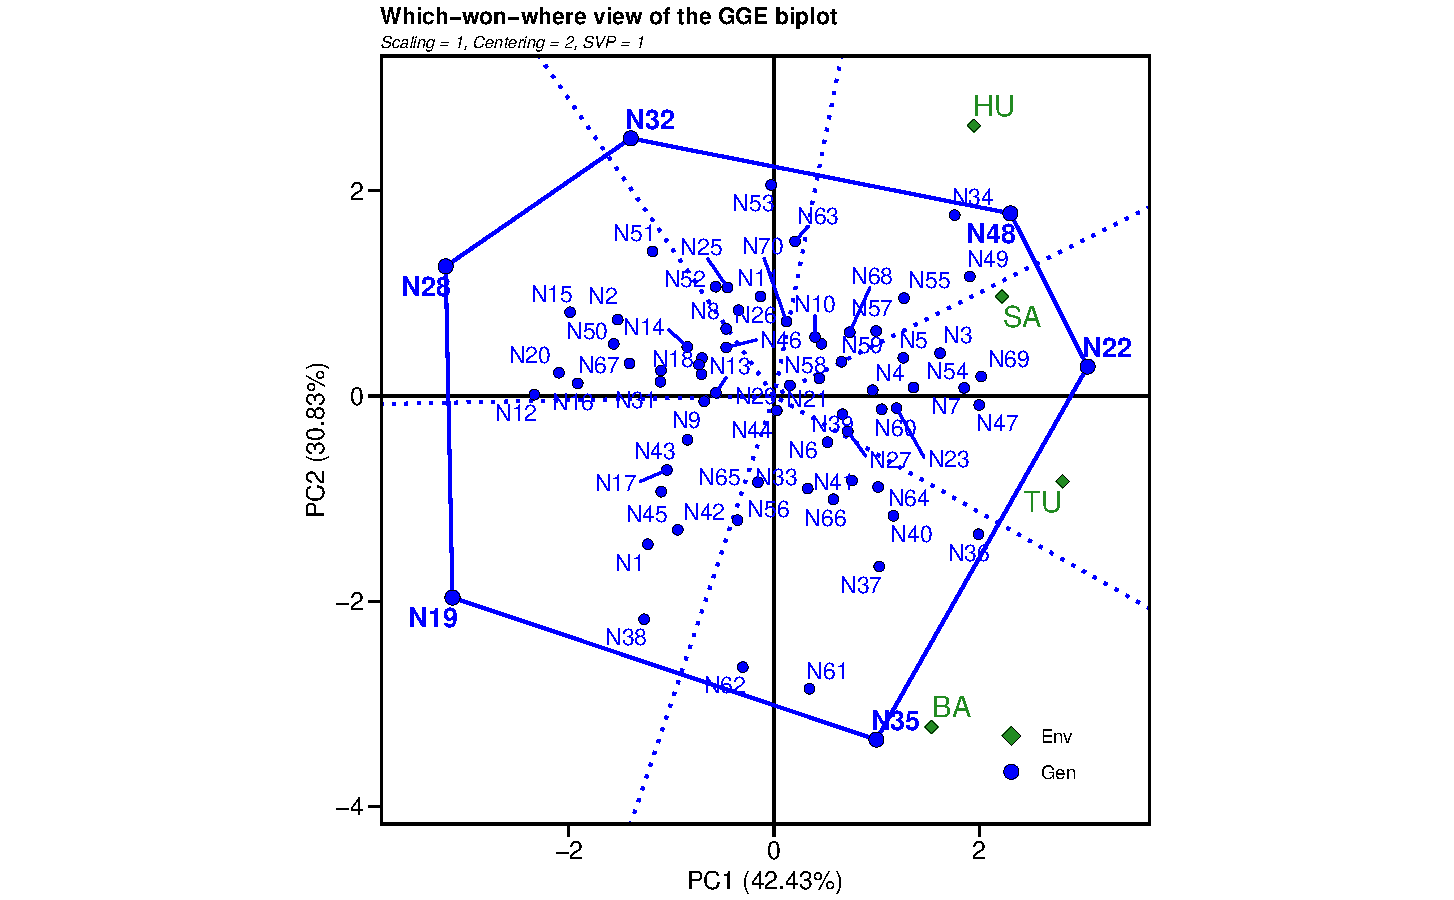
\includegraphics{figures/nb gge fig2-1} \end{center}

\hypertarget{mean-performance-and-stability-analysis-2}{%
\subsubsection{Mean performance and stability
analysis}\label{mean-performance-and-stability-analysis-2}}

WAASP index and BLUPs to estimate stability analysis.

\begin{Shaded}
\begin{Highlighting}[]
\NormalTok{waasb\_model\_nb }\OtherTok{\textless{}{-}} 
  \FunctionTok{waasb}\NormalTok{(blues\_stage.I\_NB,}
        \AttributeTok{env =}\NormalTok{ loc,}
        \AttributeTok{gen =}\NormalTok{ name,}
        \AttributeTok{rep =}\NormalTok{ rep,}
        \AttributeTok{resp =}\NormalTok{ yield,}
        \AttributeTok{random =} \StringTok{"gen"}\NormalTok{, }\CommentTok{\#Default}
        \AttributeTok{verbose =} \ConstantTok{TRUE}\NormalTok{,}
        \AttributeTok{wresp =} \DecValTok{60}\NormalTok{) }\CommentTok{\#weight for response variable 60 and 40 for yielding and stability, respectively)}
\end{Highlighting}
\end{Shaded}

\begin{verbatim}
#> Evaluating trait yield |=================================================================================================================================================================================================| 100% 00:00:04 
#> ---------------------------------------------------------------------------
#> P-values for Likelihood Ratio Test of the analyzed traits
#> ---------------------------------------------------------------------------
#>     model    yield
#>  COMPLETE       NA
#>       GEN 3.41e-05
#>   GEN:ENV 6.69e-20
#> ---------------------------------------------------------------------------
#> All variables with significant (p < 0.05) genotype-vs-environment interaction
\end{verbatim}

\begin{Shaded}
\begin{Highlighting}[]
\NormalTok{waasb\_model}\OtherTok{\textless{}{-}}\NormalTok{ waasb\_model\_nb}\SpecialCharTok{$}\NormalTok{yield}\SpecialCharTok{$}\NormalTok{model}

\NormalTok{waasp\_plot }\OtherTok{\textless{}{-}} \FunctionTok{plot\_scores}\NormalTok{(waasb\_model\_nb, }\AttributeTok{type =} \DecValTok{3}\NormalTok{,}
          \AttributeTok{title =} \ConstantTok{FALSE}\NormalTok{,}
          \AttributeTok{size.tex.gen =} \DecValTok{4}\NormalTok{,}
          \AttributeTok{size.tex.env =} \DecValTok{4}\NormalTok{,}
          \AttributeTok{size.tex.lab =} \DecValTok{13}\NormalTok{,}
         \CommentTok{\# highlight = c("N38", "N6" , "N61", "N35" ,"N52", "N22"),}
         \AttributeTok{plot\_theme =} \FunctionTok{theme\_metan}\NormalTok{(}\AttributeTok{grid =}  \StringTok{"both"}\NormalTok{,}\AttributeTok{color.background =} \FunctionTok{transparent\_color}\NormalTok{())}
\NormalTok{        ) }\SpecialCharTok{+}
  
  \FunctionTok{geom\_mark\_rect}\NormalTok{(}\FunctionTok{aes}\NormalTok{(}\AttributeTok{filter =}\NormalTok{  Code  }\SpecialCharTok{\%in\%} \FunctionTok{c}\NormalTok{(}\StringTok{"N70"}\NormalTok{, }\StringTok{"N37"}\NormalTok{, }\StringTok{"N69"}\NormalTok{, }\StringTok{"N60"}\NormalTok{),}
\NormalTok{                     ),}
               \AttributeTok{label.fontsize =} \DecValTok{10}\NormalTok{,}
               \AttributeTok{show.legend =}\NormalTok{ F,}
               \AttributeTok{con.cap =} \DecValTok{0}\NormalTok{,}
               \AttributeTok{con.colour =} \StringTok{"red"}\NormalTok{,}
               \AttributeTok{color =} \StringTok{"red"}\NormalTok{,}
               \AttributeTok{expand =} \FloatTok{0.005}\NormalTok{,}
               \AttributeTok{label.buffer =} \FunctionTok{unit}\NormalTok{(}\DecValTok{10}\NormalTok{, }\StringTok{"cm"}\NormalTok{))}\SpecialCharTok{+}
\CommentTok{\#theme\_gray()+}
\FunctionTok{theme}\NormalTok{(}\AttributeTok{legend.position =} \FunctionTok{c}\NormalTok{(}\FloatTok{0.1}\NormalTok{, }\FloatTok{0.9}\NormalTok{),}
      \AttributeTok{legend.background =} \FunctionTok{element\_blank}\NormalTok{(),}
      \AttributeTok{legend.title =} \FunctionTok{element\_blank}\NormalTok{(),}
      \AttributeTok{aspect.ratio =} \DecValTok{1}\NormalTok{) }\SpecialCharTok{+}
  \FunctionTok{labs}\NormalTok{(}\AttributeTok{x =} \StringTok{"GY"}\NormalTok{)}
\FunctionTok{print}\NormalTok{(waasp\_plot)}
\end{Highlighting}
\end{Shaded}

\begin{center}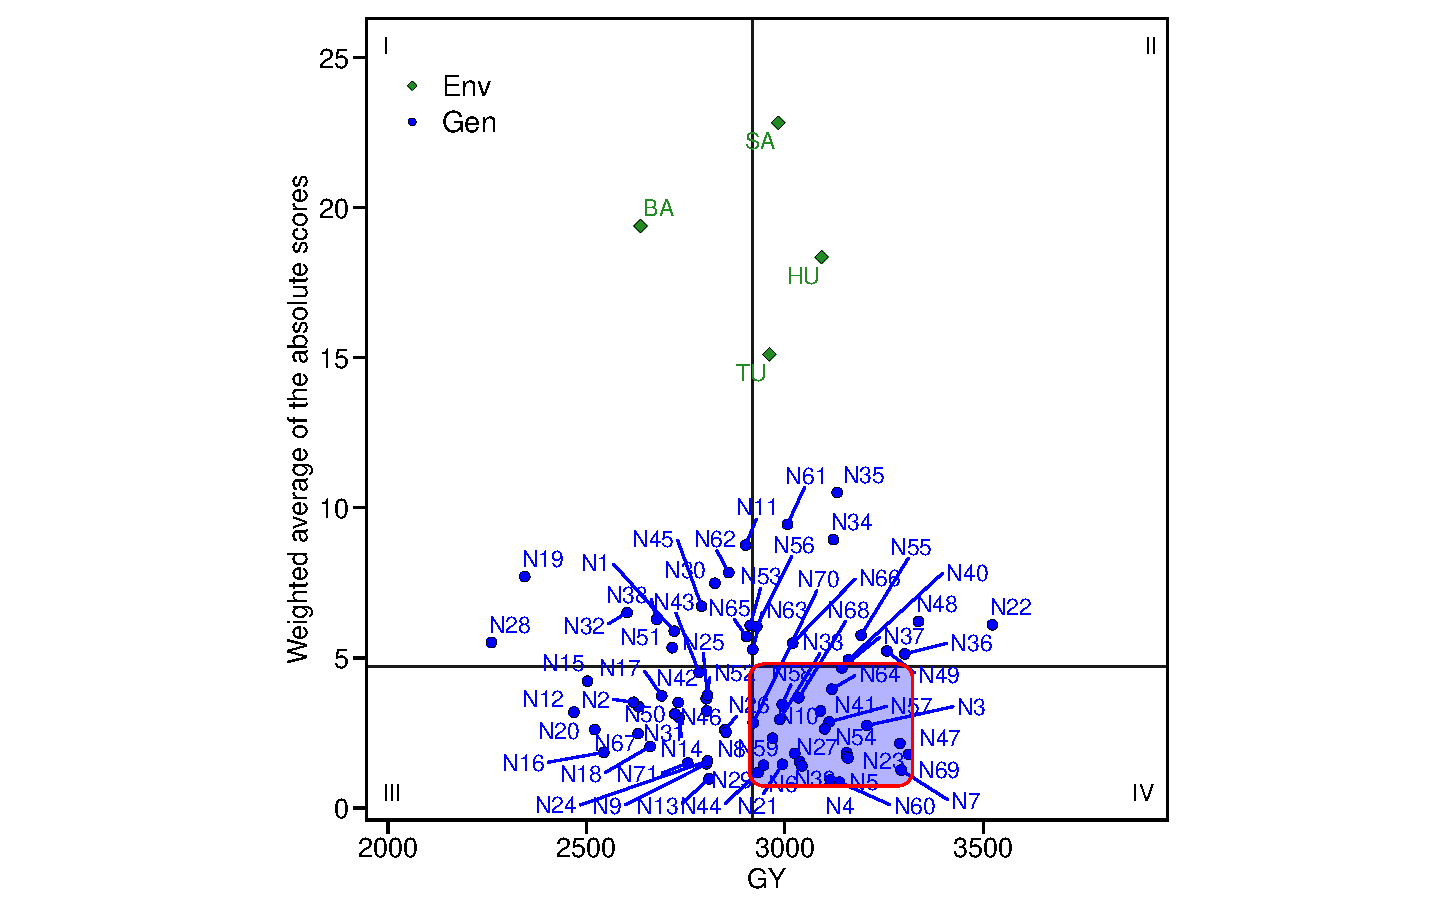
\includegraphics{figures/mod metan nb stab-1} \end{center}

\begin{Shaded}
\begin{Highlighting}[]
\NormalTok{waasb\_model\_meanWaasb}\OtherTok{\textless{}{-}}\FunctionTok{mean}\NormalTok{(waasb\_model}\SpecialCharTok{$}\NormalTok{WAASB)}
\NormalTok{waasb\_model\_meanY}\OtherTok{\textless{}{-}}\FunctionTok{mean}\NormalTok{(waasb\_model}\SpecialCharTok{$}\NormalTok{Y)}

\NormalTok{selected }\OtherTok{\textless{}{-}}\NormalTok{ waasb\_model }\SpecialCharTok{\%\textgreater{}\%}
\NormalTok{  dplyr}\SpecialCharTok{::}\FunctionTok{filter}\NormalTok{(Y }\SpecialCharTok{\textgreater{}=}\NormalTok{ waasb\_model\_meanY }\SpecialCharTok{\&}\NormalTok{ WAASB }\SpecialCharTok{\textless{}=}\NormalTok{ waasb\_model\_meanWaasb) }

\NormalTok{selected\_table }\OtherTok{\textless{}{-}}\NormalTok{ selected }

\ControlFlowTok{if}\NormalTok{ (knitr}\SpecialCharTok{::}\FunctionTok{is\_html\_output}\NormalTok{()) \{}
  
  \FunctionTok{print\_table}\NormalTok{(selected\_table)}
  
\NormalTok{\}}\ControlFlowTok{else}\NormalTok{\{}
  
\NormalTok{selected\_table[,}\DecValTok{1}\SpecialCharTok{:}\DecValTok{8}\NormalTok{]}
\NormalTok{\}}
\end{Highlighting}
\end{Shaded}

\global\setlength{\Oldarrayrulewidth}{\arrayrulewidth}

\global\setlength{\Oldtabcolsep}{\tabcolsep}

\setlength{\tabcolsep}{0pt}

\renewcommand*{\arraystretch}{1.5}



\providecommand{\ascline}[3]{\noalign{\global\arrayrulewidth #1}\arrayrulecolor[HTML]{#2}\cline{#3}}

\begin{longtable}[c]{|p{0.77in}|p{0.77in}|p{0.75in}|p{0.75in}|p{0.75in}|p{0.75in}|p{0.75in}|p{0.75in}}



\ascline{1.5pt}{666666}{1-8}

\multicolumn{1}{>{\raggedright}m{\dimexpr 0.77in+0\tabcolsep}}{\textcolor[HTML]{000000}{\fontsize{9}{9}\selectfont{\global\setmainfont{Arial}{\textbf{type}}}}} & \multicolumn{1}{>{\raggedright}m{\dimexpr 0.77in+0\tabcolsep}}{\textcolor[HTML]{000000}{\fontsize{9}{9}\selectfont{\global\setmainfont{Arial}{\textbf{Code}}}}} & \multicolumn{1}{>{\raggedleft}m{\dimexpr 0.75in+0\tabcolsep}}{\textcolor[HTML]{000000}{\fontsize{9}{9}\selectfont{\global\setmainfont{Arial}{\textbf{Y}}}}} & \multicolumn{1}{>{\raggedleft}m{\dimexpr 0.75in+0\tabcolsep}}{\textcolor[HTML]{000000}{\fontsize{9}{9}\selectfont{\global\setmainfont{Arial}{\textbf{PC1}}}}} & \multicolumn{1}{>{\raggedleft}m{\dimexpr 0.75in+0\tabcolsep}}{\textcolor[HTML]{000000}{\fontsize{9}{9}\selectfont{\global\setmainfont{Arial}{\textbf{PC2}}}}} & \multicolumn{1}{>{\raggedleft}m{\dimexpr 0.75in+0\tabcolsep}}{\textcolor[HTML]{000000}{\fontsize{9}{9}\selectfont{\global\setmainfont{Arial}{\textbf{PC3}}}}} & \multicolumn{1}{>{\raggedleft}m{\dimexpr 0.75in+0\tabcolsep}}{\textcolor[HTML]{000000}{\fontsize{9}{9}\selectfont{\global\setmainfont{Arial}{\textbf{WAASB}}}}} & \multicolumn{1}{>{\raggedleft}m{\dimexpr 0.75in+0\tabcolsep}}{\textcolor[HTML]{000000}{\fontsize{9}{9}\selectfont{\global\setmainfont{Arial}{\textbf{PctResp}}}}} \\

\ascline{0.75pt}{666666}{1-8}



\multicolumn{1}{>{\raggedright}m{\dimexpr 0.77in+0\tabcolsep}}{\textcolor[HTML]{999999}{\fontsize{9}{9}\selectfont{\global\setmainfont{Arial}{\textbf{character}}}}} & \multicolumn{1}{>{\raggedright}m{\dimexpr 0.77in+0\tabcolsep}}{\textcolor[HTML]{999999}{\fontsize{9}{9}\selectfont{\global\setmainfont{Arial}{\textbf{character}}}}} & \multicolumn{1}{>{\raggedleft}m{\dimexpr 0.75in+0\tabcolsep}}{\textcolor[HTML]{999999}{\fontsize{9}{9}\selectfont{\global\setmainfont{Arial}{\textbf{numeric}}}}} & \multicolumn{1}{>{\raggedleft}m{\dimexpr 0.75in+0\tabcolsep}}{\textcolor[HTML]{999999}{\fontsize{9}{9}\selectfont{\global\setmainfont{Arial}{\textbf{numeric}}}}} & \multicolumn{1}{>{\raggedleft}m{\dimexpr 0.75in+0\tabcolsep}}{\textcolor[HTML]{999999}{\fontsize{9}{9}\selectfont{\global\setmainfont{Arial}{\textbf{numeric}}}}} & \multicolumn{1}{>{\raggedleft}m{\dimexpr 0.75in+0\tabcolsep}}{\textcolor[HTML]{999999}{\fontsize{9}{9}\selectfont{\global\setmainfont{Arial}{\textbf{numeric}}}}} & \multicolumn{1}{>{\raggedleft}m{\dimexpr 0.75in+0\tabcolsep}}{\textcolor[HTML]{999999}{\fontsize{9}{9}\selectfont{\global\setmainfont{Arial}{\textbf{numeric}}}}} & \multicolumn{1}{>{\raggedleft}m{\dimexpr 0.75in+0\tabcolsep}}{\textcolor[HTML]{999999}{\fontsize{9}{9}\selectfont{\global\setmainfont{Arial}{\textbf{numeric}}}}} \\

\ascline{1.5pt}{666666}{1-8}\endfirsthead

\ascline{1.5pt}{666666}{1-8}

\multicolumn{1}{>{\raggedright}m{\dimexpr 0.77in+0\tabcolsep}}{\textcolor[HTML]{000000}{\fontsize{9}{9}\selectfont{\global\setmainfont{Arial}{\textbf{type}}}}} & \multicolumn{1}{>{\raggedright}m{\dimexpr 0.77in+0\tabcolsep}}{\textcolor[HTML]{000000}{\fontsize{9}{9}\selectfont{\global\setmainfont{Arial}{\textbf{Code}}}}} & \multicolumn{1}{>{\raggedleft}m{\dimexpr 0.75in+0\tabcolsep}}{\textcolor[HTML]{000000}{\fontsize{9}{9}\selectfont{\global\setmainfont{Arial}{\textbf{Y}}}}} & \multicolumn{1}{>{\raggedleft}m{\dimexpr 0.75in+0\tabcolsep}}{\textcolor[HTML]{000000}{\fontsize{9}{9}\selectfont{\global\setmainfont{Arial}{\textbf{PC1}}}}} & \multicolumn{1}{>{\raggedleft}m{\dimexpr 0.75in+0\tabcolsep}}{\textcolor[HTML]{000000}{\fontsize{9}{9}\selectfont{\global\setmainfont{Arial}{\textbf{PC2}}}}} & \multicolumn{1}{>{\raggedleft}m{\dimexpr 0.75in+0\tabcolsep}}{\textcolor[HTML]{000000}{\fontsize{9}{9}\selectfont{\global\setmainfont{Arial}{\textbf{PC3}}}}} & \multicolumn{1}{>{\raggedleft}m{\dimexpr 0.75in+0\tabcolsep}}{\textcolor[HTML]{000000}{\fontsize{9}{9}\selectfont{\global\setmainfont{Arial}{\textbf{WAASB}}}}} & \multicolumn{1}{>{\raggedleft}m{\dimexpr 0.75in+0\tabcolsep}}{\textcolor[HTML]{000000}{\fontsize{9}{9}\selectfont{\global\setmainfont{Arial}{\textbf{PctResp}}}}} \\

\ascline{0.75pt}{666666}{1-8}



\multicolumn{1}{>{\raggedright}m{\dimexpr 0.77in+0\tabcolsep}}{\textcolor[HTML]{999999}{\fontsize{9}{9}\selectfont{\global\setmainfont{Arial}{\textbf{character}}}}} & \multicolumn{1}{>{\raggedright}m{\dimexpr 0.77in+0\tabcolsep}}{\textcolor[HTML]{999999}{\fontsize{9}{9}\selectfont{\global\setmainfont{Arial}{\textbf{character}}}}} & \multicolumn{1}{>{\raggedleft}m{\dimexpr 0.75in+0\tabcolsep}}{\textcolor[HTML]{999999}{\fontsize{9}{9}\selectfont{\global\setmainfont{Arial}{\textbf{numeric}}}}} & \multicolumn{1}{>{\raggedleft}m{\dimexpr 0.75in+0\tabcolsep}}{\textcolor[HTML]{999999}{\fontsize{9}{9}\selectfont{\global\setmainfont{Arial}{\textbf{numeric}}}}} & \multicolumn{1}{>{\raggedleft}m{\dimexpr 0.75in+0\tabcolsep}}{\textcolor[HTML]{999999}{\fontsize{9}{9}\selectfont{\global\setmainfont{Arial}{\textbf{numeric}}}}} & \multicolumn{1}{>{\raggedleft}m{\dimexpr 0.75in+0\tabcolsep}}{\textcolor[HTML]{999999}{\fontsize{9}{9}\selectfont{\global\setmainfont{Arial}{\textbf{numeric}}}}} & \multicolumn{1}{>{\raggedleft}m{\dimexpr 0.75in+0\tabcolsep}}{\textcolor[HTML]{999999}{\fontsize{9}{9}\selectfont{\global\setmainfont{Arial}{\textbf{numeric}}}}} & \multicolumn{1}{>{\raggedleft}m{\dimexpr 0.75in+0\tabcolsep}}{\textcolor[HTML]{999999}{\fontsize{9}{9}\selectfont{\global\setmainfont{Arial}{\textbf{numeric}}}}} \\

\ascline{1.5pt}{666666}{1-8}\endhead



\multicolumn{8}{>{\raggedright}m{\dimexpr 6.05in+14\tabcolsep}}{\textcolor[HTML]{000000}{\fontsize{9}{9}\selectfont{\global\setmainfont{Arial}{n:\ 25}}}} \\

\ascline{0.75pt}{666666}{1-8}\endfoot



\multicolumn{1}{>{\raggedright}m{\dimexpr 0.77in+0\tabcolsep}}{\textcolor[HTML]{000000}{\fontsize{9}{9}\selectfont{\global\setmainfont{Arial}{GEN}}}} & \multicolumn{1}{>{\raggedright}m{\dimexpr 0.77in+0\tabcolsep}}{\textcolor[HTML]{000000}{\fontsize{9}{9}\selectfont{\global\setmainfont{Arial}{N10}}}} & \multicolumn{1}{>{\raggedleft}m{\dimexpr 0.75in+0\tabcolsep}}{\textcolor[HTML]{000000}{\fontsize{9}{9}\selectfont{\global\setmainfont{Arial}{2,969.3}}}} & \multicolumn{1}{>{\raggedleft}m{\dimexpr 0.75in+0\tabcolsep}}{\textcolor[HTML]{000000}{\fontsize{9}{9}\selectfont{\global\setmainfont{Arial}{3.1}}}} & \multicolumn{1}{>{\raggedleft}m{\dimexpr 0.75in+0\tabcolsep}}{\textcolor[HTML]{000000}{\fontsize{9}{9}\selectfont{\global\setmainfont{Arial}{-0.3}}}} & \multicolumn{1}{>{\raggedleft}m{\dimexpr 0.75in+0\tabcolsep}}{\textcolor[HTML]{000000}{\fontsize{9}{9}\selectfont{\global\setmainfont{Arial}{3.4}}}} & \multicolumn{1}{>{\raggedleft}m{\dimexpr 0.75in+0\tabcolsep}}{\textcolor[HTML]{000000}{\fontsize{9}{9}\selectfont{\global\setmainfont{Arial}{2.3}}}} & \multicolumn{1}{>{\raggedleft}m{\dimexpr 0.75in+0\tabcolsep}}{\textcolor[HTML]{000000}{\fontsize{9}{9}\selectfont{\global\setmainfont{Arial}{56.1}}}} \\

\ascline{0.75pt}{666666}{1-8}



\multicolumn{1}{>{\raggedright}m{\dimexpr 0.77in+0\tabcolsep}}{\textcolor[HTML]{000000}{\fontsize{9}{9}\selectfont{\global\setmainfont{Arial}{GEN}}}} & \multicolumn{1}{>{\raggedright}m{\dimexpr 0.77in+0\tabcolsep}}{\textcolor[HTML]{000000}{\fontsize{9}{9}\selectfont{\global\setmainfont{Arial}{N21}}}} & \multicolumn{1}{>{\raggedleft}m{\dimexpr 0.75in+0\tabcolsep}}{\textcolor[HTML]{000000}{\fontsize{9}{9}\selectfont{\global\setmainfont{Arial}{2,993.8}}}} & \multicolumn{1}{>{\raggedleft}m{\dimexpr 0.75in+0\tabcolsep}}{\textcolor[HTML]{000000}{\fontsize{9}{9}\selectfont{\global\setmainfont{Arial}{-0.1}}}} & \multicolumn{1}{>{\raggedleft}m{\dimexpr 0.75in+0\tabcolsep}}{\textcolor[HTML]{000000}{\fontsize{9}{9}\selectfont{\global\setmainfont{Arial}{-3.8}}}} & \multicolumn{1}{>{\raggedleft}m{\dimexpr 0.75in+0\tabcolsep}}{\textcolor[HTML]{000000}{\fontsize{9}{9}\selectfont{\global\setmainfont{Arial}{1.3}}}} & \multicolumn{1}{>{\raggedleft}m{\dimexpr 0.75in+0\tabcolsep}}{\textcolor[HTML]{000000}{\fontsize{9}{9}\selectfont{\global\setmainfont{Arial}{1.5}}}} & \multicolumn{1}{>{\raggedleft}m{\dimexpr 0.75in+0\tabcolsep}}{\textcolor[HTML]{000000}{\fontsize{9}{9}\selectfont{\global\setmainfont{Arial}{58.1}}}} \\

\ascline{0.75pt}{666666}{1-8}



\multicolumn{1}{>{\raggedright}m{\dimexpr 0.77in+0\tabcolsep}}{\textcolor[HTML]{000000}{\fontsize{9}{9}\selectfont{\global\setmainfont{Arial}{GEN}}}} & \multicolumn{1}{>{\raggedright}m{\dimexpr 0.77in+0\tabcolsep}}{\textcolor[HTML]{000000}{\fontsize{9}{9}\selectfont{\global\setmainfont{Arial}{N23}}}} & \multicolumn{1}{>{\raggedleft}m{\dimexpr 0.75in+0\tabcolsep}}{\textcolor[HTML]{000000}{\fontsize{9}{9}\selectfont{\global\setmainfont{Arial}{3,156.4}}}} & \multicolumn{1}{>{\raggedleft}m{\dimexpr 0.75in+0\tabcolsep}}{\textcolor[HTML]{000000}{\fontsize{9}{9}\selectfont{\global\setmainfont{Arial}{0.3}}}} & \multicolumn{1}{>{\raggedleft}m{\dimexpr 0.75in+0\tabcolsep}}{\textcolor[HTML]{000000}{\fontsize{9}{9}\selectfont{\global\setmainfont{Arial}{3.0}}}} & \multicolumn{1}{>{\raggedleft}m{\dimexpr 0.75in+0\tabcolsep}}{\textcolor[HTML]{000000}{\fontsize{9}{9}\selectfont{\global\setmainfont{Arial}{3.2}}}} & \multicolumn{1}{>{\raggedleft}m{\dimexpr 0.75in+0\tabcolsep}}{\textcolor[HTML]{000000}{\fontsize{9}{9}\selectfont{\global\setmainfont{Arial}{1.7}}}} & \multicolumn{1}{>{\raggedleft}m{\dimexpr 0.75in+0\tabcolsep}}{\textcolor[HTML]{000000}{\fontsize{9}{9}\selectfont{\global\setmainfont{Arial}{71.0}}}} \\

\ascline{0.75pt}{666666}{1-8}



\multicolumn{1}{>{\raggedright}m{\dimexpr 0.77in+0\tabcolsep}}{\textcolor[HTML]{000000}{\fontsize{9}{9}\selectfont{\global\setmainfont{Arial}{GEN}}}} & \multicolumn{1}{>{\raggedright}m{\dimexpr 0.77in+0\tabcolsep}}{\textcolor[HTML]{000000}{\fontsize{9}{9}\selectfont{\global\setmainfont{Arial}{N3}}}} & \multicolumn{1}{>{\raggedleft}m{\dimexpr 0.75in+0\tabcolsep}}{\textcolor[HTML]{000000}{\fontsize{9}{9}\selectfont{\global\setmainfont{Arial}{3,206.6}}}} & \multicolumn{1}{>{\raggedleft}m{\dimexpr 0.75in+0\tabcolsep}}{\textcolor[HTML]{000000}{\fontsize{9}{9}\selectfont{\global\setmainfont{Arial}{2.1}}}} & \multicolumn{1}{>{\raggedleft}m{\dimexpr 0.75in+0\tabcolsep}}{\textcolor[HTML]{000000}{\fontsize{9}{9}\selectfont{\global\setmainfont{Arial}{-1.5}}}} & \multicolumn{1}{>{\raggedleft}m{\dimexpr 0.75in+0\tabcolsep}}{\textcolor[HTML]{000000}{\fontsize{9}{9}\selectfont{\global\setmainfont{Arial}{6.2}}}} & \multicolumn{1}{>{\raggedleft}m{\dimexpr 0.75in+0\tabcolsep}}{\textcolor[HTML]{000000}{\fontsize{9}{9}\selectfont{\global\setmainfont{Arial}{2.7}}}} & \multicolumn{1}{>{\raggedleft}m{\dimexpr 0.75in+0\tabcolsep}}{\textcolor[HTML]{000000}{\fontsize{9}{9}\selectfont{\global\setmainfont{Arial}{74.9}}}} \\

\ascline{0.75pt}{666666}{1-8}



\multicolumn{1}{>{\raggedright}m{\dimexpr 0.77in+0\tabcolsep}}{\textcolor[HTML]{000000}{\fontsize{9}{9}\selectfont{\global\setmainfont{Arial}{GEN}}}} & \multicolumn{1}{>{\raggedright}m{\dimexpr 0.77in+0\tabcolsep}}{\textcolor[HTML]{000000}{\fontsize{9}{9}\selectfont{\global\setmainfont{Arial}{N33}}}} & \multicolumn{1}{>{\raggedleft}m{\dimexpr 0.75in+0\tabcolsep}}{\textcolor[HTML]{000000}{\fontsize{9}{9}\selectfont{\global\setmainfont{Arial}{2,987.3}}}} & \multicolumn{1}{>{\raggedleft}m{\dimexpr 0.75in+0\tabcolsep}}{\textcolor[HTML]{000000}{\fontsize{9}{9}\selectfont{\global\setmainfont{Arial}{-4.9}}}} & \multicolumn{1}{>{\raggedleft}m{\dimexpr 0.75in+0\tabcolsep}}{\textcolor[HTML]{000000}{\fontsize{9}{9}\selectfont{\global\setmainfont{Arial}{-0.9}}}} & \multicolumn{1}{>{\raggedleft}m{\dimexpr 0.75in+0\tabcolsep}}{\textcolor[HTML]{000000}{\fontsize{9}{9}\selectfont{\global\setmainfont{Arial}{1.3}}}} & \multicolumn{1}{>{\raggedleft}m{\dimexpr 0.75in+0\tabcolsep}}{\textcolor[HTML]{000000}{\fontsize{9}{9}\selectfont{\global\setmainfont{Arial}{2.9}}}} & \multicolumn{1}{>{\raggedleft}m{\dimexpr 0.75in+0\tabcolsep}}{\textcolor[HTML]{000000}{\fontsize{9}{9}\selectfont{\global\setmainfont{Arial}{57.6}}}} \\

\ascline{0.75pt}{666666}{1-8}



\multicolumn{1}{>{\raggedright}m{\dimexpr 0.77in+0\tabcolsep}}{\textcolor[HTML]{000000}{\fontsize{9}{9}\selectfont{\global\setmainfont{Arial}{GEN}}}} & \multicolumn{1}{>{\raggedright}m{\dimexpr 0.77in+0\tabcolsep}}{\textcolor[HTML]{000000}{\fontsize{9}{9}\selectfont{\global\setmainfont{Arial}{N37}}}} & \multicolumn{1}{>{\raggedleft}m{\dimexpr 0.75in+0\tabcolsep}}{\textcolor[HTML]{000000}{\fontsize{9}{9}\selectfont{\global\setmainfont{Arial}{3,143.7}}}} & \multicolumn{1}{>{\raggedleft}m{\dimexpr 0.75in+0\tabcolsep}}{\textcolor[HTML]{000000}{\fontsize{9}{9}\selectfont{\global\setmainfont{Arial}{-8.6}}}} & \multicolumn{1}{>{\raggedleft}m{\dimexpr 0.75in+0\tabcolsep}}{\textcolor[HTML]{000000}{\fontsize{9}{9}\selectfont{\global\setmainfont{Arial}{0.3}}}} & \multicolumn{1}{>{\raggedleft}m{\dimexpr 0.75in+0\tabcolsep}}{\textcolor[HTML]{000000}{\fontsize{9}{9}\selectfont{\global\setmainfont{Arial}{1.9}}}} & \multicolumn{1}{>{\raggedleft}m{\dimexpr 0.75in+0\tabcolsep}}{\textcolor[HTML]{000000}{\fontsize{9}{9}\selectfont{\global\setmainfont{Arial}{4.7}}}} & \multicolumn{1}{>{\raggedleft}m{\dimexpr 0.75in+0\tabcolsep}}{\textcolor[HTML]{000000}{\fontsize{9}{9}\selectfont{\global\setmainfont{Arial}{70.0}}}} \\

\ascline{0.75pt}{666666}{1-8}



\multicolumn{1}{>{\raggedright}m{\dimexpr 0.77in+0\tabcolsep}}{\textcolor[HTML]{000000}{\fontsize{9}{9}\selectfont{\global\setmainfont{Arial}{GEN}}}} & \multicolumn{1}{>{\raggedright}m{\dimexpr 0.77in+0\tabcolsep}}{\textcolor[HTML]{000000}{\fontsize{9}{9}\selectfont{\global\setmainfont{Arial}{N39}}}} & \multicolumn{1}{>{\raggedleft}m{\dimexpr 0.75in+0\tabcolsep}}{\textcolor[HTML]{000000}{\fontsize{9}{9}\selectfont{\global\setmainfont{Arial}{3,037.0}}}} & \multicolumn{1}{>{\raggedleft}m{\dimexpr 0.75in+0\tabcolsep}}{\textcolor[HTML]{000000}{\fontsize{9}{9}\selectfont{\global\setmainfont{Arial}{-1.1}}}} & \multicolumn{1}{>{\raggedleft}m{\dimexpr 0.75in+0\tabcolsep}}{\textcolor[HTML]{000000}{\fontsize{9}{9}\selectfont{\global\setmainfont{Arial}{-1.3}}}} & \multicolumn{1}{>{\raggedleft}m{\dimexpr 0.75in+0\tabcolsep}}{\textcolor[HTML]{000000}{\fontsize{9}{9}\selectfont{\global\setmainfont{Arial}{3.0}}}} & \multicolumn{1}{>{\raggedleft}m{\dimexpr 0.75in+0\tabcolsep}}{\textcolor[HTML]{000000}{\fontsize{9}{9}\selectfont{\global\setmainfont{Arial}{1.5}}}} & \multicolumn{1}{>{\raggedleft}m{\dimexpr 0.75in+0\tabcolsep}}{\textcolor[HTML]{000000}{\fontsize{9}{9}\selectfont{\global\setmainfont{Arial}{61.5}}}} \\

\ascline{0.75pt}{666666}{1-8}



\multicolumn{1}{>{\raggedright}m{\dimexpr 0.77in+0\tabcolsep}}{\textcolor[HTML]{000000}{\fontsize{9}{9}\selectfont{\global\setmainfont{Arial}{GEN}}}} & \multicolumn{1}{>{\raggedright}m{\dimexpr 0.77in+0\tabcolsep}}{\textcolor[HTML]{000000}{\fontsize{9}{9}\selectfont{\global\setmainfont{Arial}{N4}}}} & \multicolumn{1}{>{\raggedleft}m{\dimexpr 0.75in+0\tabcolsep}}{\textcolor[HTML]{000000}{\fontsize{9}{9}\selectfont{\global\setmainfont{Arial}{3,114.3}}}} & \multicolumn{1}{>{\raggedleft}m{\dimexpr 0.75in+0\tabcolsep}}{\textcolor[HTML]{000000}{\fontsize{9}{9}\selectfont{\global\setmainfont{Arial}{-0.3}}}} & \multicolumn{1}{>{\raggedleft}m{\dimexpr 0.75in+0\tabcolsep}}{\textcolor[HTML]{000000}{\fontsize{9}{9}\selectfont{\global\setmainfont{Arial}{-2.1}}}} & \multicolumn{1}{>{\raggedleft}m{\dimexpr 0.75in+0\tabcolsep}}{\textcolor[HTML]{000000}{\fontsize{9}{9}\selectfont{\global\setmainfont{Arial}{0.8}}}} & \multicolumn{1}{>{\raggedleft}m{\dimexpr 0.75in+0\tabcolsep}}{\textcolor[HTML]{000000}{\fontsize{9}{9}\selectfont{\global\setmainfont{Arial}{0.9}}}} & \multicolumn{1}{>{\raggedleft}m{\dimexpr 0.75in+0\tabcolsep}}{\textcolor[HTML]{000000}{\fontsize{9}{9}\selectfont{\global\setmainfont{Arial}{67.6}}}} \\

\ascline{0.75pt}{666666}{1-8}



\multicolumn{1}{>{\raggedright}m{\dimexpr 0.77in+0\tabcolsep}}{\textcolor[HTML]{000000}{\fontsize{9}{9}\selectfont{\global\setmainfont{Arial}{GEN}}}} & \multicolumn{1}{>{\raggedright}m{\dimexpr 0.77in+0\tabcolsep}}{\textcolor[HTML]{000000}{\fontsize{9}{9}\selectfont{\global\setmainfont{Arial}{N41}}}} & \multicolumn{1}{>{\raggedleft}m{\dimexpr 0.75in+0\tabcolsep}}{\textcolor[HTML]{000000}{\fontsize{9}{9}\selectfont{\global\setmainfont{Arial}{3,090.0}}}} & \multicolumn{1}{>{\raggedleft}m{\dimexpr 0.75in+0\tabcolsep}}{\textcolor[HTML]{000000}{\fontsize{9}{9}\selectfont{\global\setmainfont{Arial}{-3.0}}}} & \multicolumn{1}{>{\raggedleft}m{\dimexpr 0.75in+0\tabcolsep}}{\textcolor[HTML]{000000}{\fontsize{9}{9}\selectfont{\global\setmainfont{Arial}{4.8}}}} & \multicolumn{1}{>{\raggedleft}m{\dimexpr 0.75in+0\tabcolsep}}{\textcolor[HTML]{000000}{\fontsize{9}{9}\selectfont{\global\setmainfont{Arial}{1.4}}}} & \multicolumn{1}{>{\raggedleft}m{\dimexpr 0.75in+0\tabcolsep}}{\textcolor[HTML]{000000}{\fontsize{9}{9}\selectfont{\global\setmainfont{Arial}{3.2}}}} & \multicolumn{1}{>{\raggedleft}m{\dimexpr 0.75in+0\tabcolsep}}{\textcolor[HTML]{000000}{\fontsize{9}{9}\selectfont{\global\setmainfont{Arial}{65.7}}}} \\

\ascline{1.5pt}{666666}{1-8}



\end{longtable}



\arrayrulecolor[HTML]{000000}

\global\setlength{\arrayrulewidth}{\Oldarrayrulewidth}

\global\setlength{\tabcolsep}{\Oldtabcolsep}

\renewcommand*{\arraystretch}{1}

\begin{Shaded}
\begin{Highlighting}[]
\CommentTok{\#selected$Code}
\end{Highlighting}
\end{Shaded}

\hypertarget{selection-differentials-2}{%
\paragraph{Selection differentials}\label{selection-differentials-2}}

\begin{Shaded}
\begin{Highlighting}[]
\CommentTok{\#Create a data frame with BLUPS {-} selected and non{-}selected}
\NormalTok{blups\_sel }\OtherTok{\textless{}{-}}
  \FunctionTok{gmd}\NormalTok{(waasb\_model\_nb, }\StringTok{"blupge"}\NormalTok{) }\SpecialCharTok{\%\textgreater{}\%}
  \FunctionTok{add\_cols}\NormalTok{(}\AttributeTok{SELECTED =} \FunctionTok{ifelse}\NormalTok{(GEN }\SpecialCharTok{\%in\%}\NormalTok{ selected}\SpecialCharTok{$}\NormalTok{Code, }\StringTok{"yes"}\NormalTok{, }\StringTok{"no"}\NormalTok{)) }\SpecialCharTok{\%\textgreater{}\%} 
\NormalTok{    dplyr}\SpecialCharTok{::}\FunctionTok{rename}\NormalTok{(}\AttributeTok{BLUPs\_sel =}\NormalTok{ yield) }\SpecialCharTok{\%\textgreater{}\%} 
  \FunctionTok{droplevels}\NormalTok{()}

\NormalTok{blups\_sel\_mean}\OtherTok{\textless{}{-}}
  \FunctionTok{gmd}\NormalTok{(waasb\_model\_nb, }\StringTok{"blupge"}\NormalTok{) }\SpecialCharTok{\%\textgreater{}\%}
  \FunctionTok{add\_cols}\NormalTok{(}\AttributeTok{SELECTED =} \FunctionTok{ifelse}\NormalTok{(GEN }\SpecialCharTok{\%in\%}\NormalTok{ selected}\SpecialCharTok{$}\NormalTok{Code, }\StringTok{"yes"}\NormalTok{, }\StringTok{"no"}\NormalTok{)) }\SpecialCharTok{\%\textgreater{}\%} 
  \FunctionTok{filter}\NormalTok{(SELECTED }\SpecialCharTok{==} \StringTok{"yes"}\NormalTok{) }\SpecialCharTok{\%\textgreater{}\%} 
\NormalTok{  dplyr}\SpecialCharTok{::}\FunctionTok{summarise}\NormalTok{(}\AttributeTok{mean\_GY =} \FunctionTok{mean}\NormalTok{(yield,}\AttributeTok{na.rm =} \ConstantTok{TRUE}\NormalTok{), }\AttributeTok{n =} \FunctionTok{n}\NormalTok{()) }

\CommentTok{\# Create a data frame with the waasb index {-} selected and non{-}selected}
\NormalTok{waasb\_sel }\OtherTok{\textless{}{-}}
  \FunctionTok{gmd}\NormalTok{(waasb\_model\_nb, }\StringTok{"WAASB"}\NormalTok{) }\SpecialCharTok{\%\textgreater{}\%}
  \FunctionTok{add\_cols}\NormalTok{(}\AttributeTok{SELECTED =} \FunctionTok{ifelse}\NormalTok{(GEN }\SpecialCharTok{\%in\%}\NormalTok{ selected}\SpecialCharTok{$}\NormalTok{Code, }\StringTok{"yes"}\NormalTok{, }\StringTok{"no"}\NormalTok{)) }\SpecialCharTok{\%\textgreater{}\%} 
\NormalTok{  dplyr}\SpecialCharTok{::}\FunctionTok{rename}\NormalTok{(}\AttributeTok{WAASB\_sel =}\NormalTok{ yield) }\SpecialCharTok{\%\textgreater{}\%} 
  \FunctionTok{droplevels}\NormalTok{()}
\CommentTok{\#str(waasb\_sel)}

\NormalTok{waasb\_sel\_mean}\OtherTok{\textless{}{-}}
  \FunctionTok{gmd}\NormalTok{(waasb\_model\_nb, }\StringTok{"WAASB"}\NormalTok{) }\SpecialCharTok{\%\textgreater{}\%}
  \FunctionTok{add\_cols}\NormalTok{(}\AttributeTok{SELECTED =} \FunctionTok{ifelse}\NormalTok{(GEN }\SpecialCharTok{\%in\%}\NormalTok{ selected}\SpecialCharTok{$}\NormalTok{Code, }\StringTok{"yes"}\NormalTok{, }\StringTok{"no"}\NormalTok{)) }\SpecialCharTok{\%\textgreater{}\%} 
  \FunctionTok{filter}\NormalTok{(SELECTED }\SpecialCharTok{==} \StringTok{"yes"}\NormalTok{) }\SpecialCharTok{\%\textgreater{}\%} 
\NormalTok{  dplyr}\SpecialCharTok{::}\FunctionTok{summarise}\NormalTok{(}\AttributeTok{mean\_GY =} \FunctionTok{mean}\NormalTok{(yield,}\AttributeTok{na.rm =} \ConstantTok{TRUE}\NormalTok{), }\AttributeTok{n =} \FunctionTok{n}\NormalTok{()) }

\NormalTok{p1}\OtherTok{\textless{}{-}} \FunctionTok{plot\_selected}\NormalTok{(blups\_sel, GEN, BLUPs\_sel, }\AttributeTok{mean\_sel =}\NormalTok{ blups\_sel\_mean}\SpecialCharTok{$}\NormalTok{mean\_GY) }\SpecialCharTok{+}
  \FunctionTok{labs}\NormalTok{(}\AttributeTok{y =} \StringTok{"GY"}\NormalTok{)}

\NormalTok{p3}\OtherTok{\textless{}{-}} \FunctionTok{plot\_selected}\NormalTok{(waasb\_sel, GEN, WAASB\_sel, }\AttributeTok{mean\_sel =}\NormalTok{ waasb\_sel\_mean}\SpecialCharTok{$}\NormalTok{mean\_GY) }\SpecialCharTok{+}
  \FunctionTok{labs}\NormalTok{(}\AttributeTok{y =} \StringTok{"WAASB index"}\NormalTok{)}

\FunctionTok{arrange\_ggplot}\NormalTok{(p1, p3,}
  \AttributeTok{guides =} \StringTok{"collect"}\NormalTok{,}
  \AttributeTok{tag\_levels =} \StringTok{"a"}\NormalTok{,}
  \AttributeTok{tag\_prefix =} \StringTok{"("}\NormalTok{,}
  \AttributeTok{tag\_suffix =} \StringTok{")"}\NormalTok{)}
\end{Highlighting}
\end{Shaded}

\begin{figure}

{\centering \includegraphics{figures/mod metan nb stab2-1} 

}

\caption{Mean performance (a) and stability (b) for grain yield (GY) of 71 Navy beans genotypes. The vertical dashed and solid lines shows, respectivelly, the  mean of the selected genotype and the overall mean for both mean performance and WAASB index}\label{fig:mod metan nb stab2}
\end{figure}

Percentage (SD\_gain in \%) gain from the selected genotypes compared to
the general mean.

\begin{Shaded}
\begin{Highlighting}[]
\NormalTok{blups\_sel2 }\OtherTok{\textless{}{-}}
  \FunctionTok{gmd}\NormalTok{(waasb\_model\_nb, }\StringTok{"blupg"}\NormalTok{) }\SpecialCharTok{\%\textgreater{}\%}
  \FunctionTok{add\_cols}\NormalTok{(}\AttributeTok{SELECTED =} \FunctionTok{ifelse}\NormalTok{(GEN }\SpecialCharTok{\%in\%}\NormalTok{ selected}\SpecialCharTok{$}\NormalTok{Code, }\StringTok{"yes"}\NormalTok{, }\StringTok{"no"}\NormalTok{)) }\SpecialCharTok{\%\textgreater{}\%} 
\NormalTok{    dplyr}\SpecialCharTok{::}\FunctionTok{rename}\NormalTok{(}\AttributeTok{BLUPs\_sel =}\NormalTok{ yield) }\SpecialCharTok{\%\textgreater{}\%} 
  \FunctionTok{droplevels}\NormalTok{()}
\end{Highlighting}
\end{Shaded}

\begin{verbatim}
#> Class of the model: waasb
\end{verbatim}

\begin{verbatim}
#> Variable extracted: blupg
\end{verbatim}

\begin{Shaded}
\begin{Highlighting}[]
\NormalTok{blups\_sel\_mean2}\OtherTok{\textless{}{-}}
  \FunctionTok{gmd}\NormalTok{(waasb\_model\_nb, }\StringTok{"blupg"}\NormalTok{) }\SpecialCharTok{\%\textgreater{}\%}
  \FunctionTok{add\_cols}\NormalTok{(}\AttributeTok{SELECTED =} \FunctionTok{ifelse}\NormalTok{(GEN }\SpecialCharTok{\%in\%}\NormalTok{ selected}\SpecialCharTok{$}\NormalTok{Code, }\StringTok{"yes"}\NormalTok{, }\StringTok{"no"}\NormalTok{)) }\SpecialCharTok{\%\textgreater{}\%} 
  \FunctionTok{filter}\NormalTok{(SELECTED }\SpecialCharTok{==} \StringTok{"yes"}\NormalTok{) }\SpecialCharTok{\%\textgreater{}\%} 
\NormalTok{  dplyr}\SpecialCharTok{::}\FunctionTok{summarise}\NormalTok{(}\AttributeTok{mean\_GY =} \FunctionTok{mean}\NormalTok{(yield,}\AttributeTok{na.rm =} \ConstantTok{TRUE}\NormalTok{), }\AttributeTok{n =} \FunctionTok{n}\NormalTok{()) }
\end{Highlighting}
\end{Shaded}

\begin{verbatim}
#> Class of the model: waasb
#> Variable extracted: blupg
\end{verbatim}

\begin{Shaded}
\begin{Highlighting}[]
\NormalTok{SD\_blups}\OtherTok{\textless{}{-}} \FunctionTok{as\_tibble}\NormalTok{((blups\_sel\_mean2}\SpecialCharTok{$}\NormalTok{mean\_GY}\SpecialCharTok{/}\FunctionTok{mean}\NormalTok{(blups\_sel2}\SpecialCharTok{$}\NormalTok{BLUPs\_sel, }\AttributeTok{na.rm =}\NormalTok{ T)) }\SpecialCharTok{{-}}\DecValTok{1}\NormalTok{)}\SpecialCharTok{*}\DecValTok{100}
\NormalTok{SD\_WAASP}\OtherTok{\textless{}{-}} \FunctionTok{as\_tibble}\NormalTok{((waasb\_sel\_mean}\SpecialCharTok{$}\NormalTok{mean\_GY }\SpecialCharTok{/}\FunctionTok{mean}\NormalTok{(waasb\_sel}\SpecialCharTok{$}\NormalTok{WAASB\_sel, }\AttributeTok{na.rm =}\NormalTok{ T)) }\SpecialCharTok{{-}}\DecValTok{1}\NormalTok{)}\SpecialCharTok{*}\DecValTok{100}

\NormalTok{SD\_comb}\OtherTok{\textless{}{-}} \FunctionTok{full\_join}\NormalTok{(SD\_blups, SD\_WAASP, }\AttributeTok{by =} \StringTok{"value"}\NormalTok{) }\SpecialCharTok{\%\textgreater{}\%} 
\NormalTok{  dplyr}\SpecialCharTok{::}\FunctionTok{rename}\NormalTok{(}\AttributeTok{SD\_gain =}\NormalTok{ value) }\SpecialCharTok{\%\textgreater{}\%} 
\NormalTok{  tibble}\SpecialCharTok{::}\FunctionTok{add\_column}\NormalTok{(}\AttributeTok{Comp\_name =} \FunctionTok{c}\NormalTok{(}\StringTok{\textquotesingle{}BLUPs\textquotesingle{}}\NormalTok{, }\StringTok{\textquotesingle{}WAASB\textquotesingle{}}\NormalTok{)) }\SpecialCharTok{\%\textgreater{}\%} 
  \FunctionTok{relocate}\NormalTok{(Comp\_name)}

\NormalTok{SD\_comb}\SpecialCharTok{$}\NormalTok{n\_selected}\OtherTok{\textless{}{-}}\NormalTok{ blups\_sel\_mean2}\SpecialCharTok{$}\NormalTok{n}
\NormalTok{SD\_comb}
\end{Highlighting}
\end{Shaded}

\global\setlength{\Oldarrayrulewidth}{\arrayrulewidth}

\global\setlength{\Oldtabcolsep}{\tabcolsep}

\setlength{\tabcolsep}{0pt}

\renewcommand*{\arraystretch}{1.5}



\providecommand{\ascline}[3]{\noalign{\global\arrayrulewidth #1}\arrayrulecolor[HTML]{#2}\cline{#3}}

\begin{longtable}[c]{|p{0.96in}|p{0.75in}|p{0.86in}}



\ascline{1.5pt}{666666}{1-3}

\multicolumn{1}{>{\raggedright}m{\dimexpr 0.96in+0\tabcolsep}}{\textcolor[HTML]{000000}{\fontsize{9}{9}\selectfont{\global\setmainfont{Arial}{\textbf{Comp\_name}}}}} & \multicolumn{1}{>{\raggedleft}m{\dimexpr 0.75in+0\tabcolsep}}{\textcolor[HTML]{000000}{\fontsize{9}{9}\selectfont{\global\setmainfont{Arial}{\textbf{SD\_gain}}}}} & \multicolumn{1}{>{\raggedleft}m{\dimexpr 0.86in+0\tabcolsep}}{\textcolor[HTML]{000000}{\fontsize{9}{9}\selectfont{\global\setmainfont{Arial}{\textbf{n\_selected}}}}} \\

\ascline{0.75pt}{666666}{1-3}



\multicolumn{1}{>{\raggedright}m{\dimexpr 0.96in+0\tabcolsep}}{\textcolor[HTML]{999999}{\fontsize{9}{9}\selectfont{\global\setmainfont{Arial}{\textbf{character}}}}} & \multicolumn{1}{>{\raggedleft}m{\dimexpr 0.75in+0\tabcolsep}}{\textcolor[HTML]{999999}{\fontsize{9}{9}\selectfont{\global\setmainfont{Arial}{\textbf{numeric}}}}} & \multicolumn{1}{>{\raggedleft}m{\dimexpr 0.86in+0\tabcolsep}}{\textcolor[HTML]{999999}{\fontsize{9}{9}\selectfont{\global\setmainfont{Arial}{\textbf{integer}}}}} \\

\ascline{1.5pt}{666666}{1-3}\endfirsthead

\ascline{1.5pt}{666666}{1-3}

\multicolumn{1}{>{\raggedright}m{\dimexpr 0.96in+0\tabcolsep}}{\textcolor[HTML]{000000}{\fontsize{9}{9}\selectfont{\global\setmainfont{Arial}{\textbf{Comp\_name}}}}} & \multicolumn{1}{>{\raggedleft}m{\dimexpr 0.75in+0\tabcolsep}}{\textcolor[HTML]{000000}{\fontsize{9}{9}\selectfont{\global\setmainfont{Arial}{\textbf{SD\_gain}}}}} & \multicolumn{1}{>{\raggedleft}m{\dimexpr 0.86in+0\tabcolsep}}{\textcolor[HTML]{000000}{\fontsize{9}{9}\selectfont{\global\setmainfont{Arial}{\textbf{n\_selected}}}}} \\

\ascline{0.75pt}{666666}{1-3}



\multicolumn{1}{>{\raggedright}m{\dimexpr 0.96in+0\tabcolsep}}{\textcolor[HTML]{999999}{\fontsize{9}{9}\selectfont{\global\setmainfont{Arial}{\textbf{character}}}}} & \multicolumn{1}{>{\raggedleft}m{\dimexpr 0.75in+0\tabcolsep}}{\textcolor[HTML]{999999}{\fontsize{9}{9}\selectfont{\global\setmainfont{Arial}{\textbf{numeric}}}}} & \multicolumn{1}{>{\raggedleft}m{\dimexpr 0.86in+0\tabcolsep}}{\textcolor[HTML]{999999}{\fontsize{9}{9}\selectfont{\global\setmainfont{Arial}{\textbf{integer}}}}} \\

\ascline{1.5pt}{666666}{1-3}\endhead



\multicolumn{3}{>{\raggedright}m{\dimexpr 2.57in+4\tabcolsep}}{\textcolor[HTML]{000000}{\fontsize{9}{9}\selectfont{\global\setmainfont{Arial}{n:\ 2}}}} \\

\ascline{0.75pt}{666666}{1-3}\endfoot



\multicolumn{1}{>{\raggedright}m{\dimexpr 0.96in+0\tabcolsep}}{\textcolor[HTML]{000000}{\fontsize{9}{9}\selectfont{\global\setmainfont{Arial}{BLUPs}}}} & \multicolumn{1}{>{\raggedleft}m{\dimexpr 0.75in+0\tabcolsep}}{\textcolor[HTML]{000000}{\fontsize{9}{9}\selectfont{\global\setmainfont{Arial}{3.2}}}} & \multicolumn{1}{>{\raggedleft}m{\dimexpr 0.86in+0\tabcolsep}}{\textcolor[HTML]{000000}{\fontsize{9}{9}\selectfont{\global\setmainfont{Arial}{25}}}} \\

\ascline{0.75pt}{666666}{1-3}



\multicolumn{1}{>{\raggedright}m{\dimexpr 0.96in+0\tabcolsep}}{\textcolor[HTML]{000000}{\fontsize{9}{9}\selectfont{\global\setmainfont{Arial}{WAASB}}}} & \multicolumn{1}{>{\raggedleft}m{\dimexpr 0.75in+0\tabcolsep}}{\textcolor[HTML]{000000}{\fontsize{9}{9}\selectfont{\global\setmainfont{Arial}{-42.4}}}} & \multicolumn{1}{>{\raggedleft}m{\dimexpr 0.86in+0\tabcolsep}}{\textcolor[HTML]{000000}{\fontsize{9}{9}\selectfont{\global\setmainfont{Arial}{25}}}} \\

\ascline{1.5pt}{666666}{1-3}



\end{longtable}



\arrayrulecolor[HTML]{000000}

\global\setlength{\arrayrulewidth}{\Oldarrayrulewidth}

\global\setlength{\tabcolsep}{\Oldtabcolsep}

\renewcommand*{\arraystretch}{1}

\begin{Shaded}
\begin{Highlighting}[]
\NormalTok{blups\_sel2}\SpecialCharTok{$}\NormalTok{mean\_blup }\OtherTok{\textless{}{-}} \FunctionTok{mean}\NormalTok{(blups\_sel2}\SpecialCharTok{$}\NormalTok{BLUPs\_sel, }\AttributeTok{na.rm =}\NormalTok{ T)}
\NormalTok{waasb\_sel}\SpecialCharTok{$}\NormalTok{mean\_waasb }\OtherTok{\textless{}{-}} \FunctionTok{mean}\NormalTok{(waasb\_sel}\SpecialCharTok{$}\NormalTok{WAASB\_sel, }\AttributeTok{na.rm =}\NormalTok{ T)}

\CommentTok{\#str(waasb\_sel)}
\NormalTok{data\_comb}\OtherTok{\textless{}{-}} \FunctionTok{merge}\NormalTok{(blups\_sel2, waasb\_sel, }\AttributeTok{by =} \FunctionTok{c}\NormalTok{(}\StringTok{"GEN"}\NormalTok{, }\StringTok{"SELECTED"}\NormalTok{))}
\CommentTok{\#names(data\_comb)}
\DocumentationTok{\#\# SD for each genotype}
\NormalTok{data\_sel\_perc }\OtherTok{\textless{}{-}}\NormalTok{ data\_comb }\SpecialCharTok{\%\textgreater{}\%}
\NormalTok{ rowwise }\SpecialCharTok{\%\textgreater{}\%}
  \FunctionTok{mutate}\NormalTok{(}\AttributeTok{Perc\_blup\_gain =}\NormalTok{ ((BLUPs\_sel}\SpecialCharTok{/}\NormalTok{mean\_blup)}\SpecialCharTok{*}\DecValTok{100}\NormalTok{)}\SpecialCharTok{{-}}\DecValTok{100}\NormalTok{) }\SpecialCharTok{\%\textgreater{}\%} 
  \FunctionTok{mutate}\NormalTok{(}\AttributeTok{Perc\_WAASB\_gain =}\NormalTok{ ((WAASB\_sel}\SpecialCharTok{/}\NormalTok{mean\_waasb)}\SpecialCharTok{*}\DecValTok{100}\NormalTok{)}\SpecialCharTok{{-}}\DecValTok{100}\NormalTok{) }\SpecialCharTok{\%\textgreater{}\%} 
  \FunctionTok{as\_tibble}\NormalTok{()}

\CommentTok{\# data\_sel\_perc\_mean \textless{}{-} data\_sel\_perc \%\textgreater{}\% }
\CommentTok{\#   dplyr::filter(SELECTED  == "yes")}
\CommentTok{\# }
\CommentTok{\# mean(data\_sel\_perc\_mean$Perc\_blup\_gain)}

\ControlFlowTok{if}\NormalTok{ (knitr}\SpecialCharTok{::}\FunctionTok{is\_html\_output}\NormalTok{()) \{}
  
  \FunctionTok{print\_table}\NormalTok{(data\_sel\_perc)}
  
\NormalTok{\}}\ControlFlowTok{else}\NormalTok{\{}
  
\NormalTok{data\_sel\_perc[,}\DecValTok{1}\SpecialCharTok{:}\DecValTok{7}\NormalTok{]}
\NormalTok{\}}
\end{Highlighting}
\end{Shaded}

\global\setlength{\Oldarrayrulewidth}{\arrayrulewidth}

\global\setlength{\Oldtabcolsep}{\tabcolsep}

\setlength{\tabcolsep}{0pt}

\renewcommand*{\arraystretch}{1.5}



\providecommand{\ascline}[3]{\noalign{\global\arrayrulewidth #1}\arrayrulecolor[HTML]{#2}\cline{#3}}

\begin{longtable}[c]{|p{0.77in}|p{0.88in}|p{0.86in}|p{0.87in}|p{0.93in}|p{0.99in}|p{1.14in}}



\ascline{1.5pt}{666666}{1-7}

\multicolumn{1}{>{\raggedright}m{\dimexpr 0.77in+0\tabcolsep}}{\textcolor[HTML]{000000}{\fontsize{9}{9}\selectfont{\global\setmainfont{Arial}{\textbf{GEN}}}}} & \multicolumn{1}{>{\raggedright}m{\dimexpr 0.88in+0\tabcolsep}}{\textcolor[HTML]{000000}{\fontsize{9}{9}\selectfont{\global\setmainfont{Arial}{\textbf{SELECTED}}}}} & \multicolumn{1}{>{\raggedleft}m{\dimexpr 0.86in+0\tabcolsep}}{\textcolor[HTML]{000000}{\fontsize{9}{9}\selectfont{\global\setmainfont{Arial}{\textbf{BLUPs\_sel}}}}} & \multicolumn{1}{>{\raggedleft}m{\dimexpr 0.87in+0\tabcolsep}}{\textcolor[HTML]{000000}{\fontsize{9}{9}\selectfont{\global\setmainfont{Arial}{\textbf{mean\_blup}}}}} & \multicolumn{1}{>{\raggedleft}m{\dimexpr 0.93in+0\tabcolsep}}{\textcolor[HTML]{000000}{\fontsize{9}{9}\selectfont{\global\setmainfont{Arial}{\textbf{WAASB\_sel}}}}} & \multicolumn{1}{>{\raggedleft}m{\dimexpr 0.99in+0\tabcolsep}}{\textcolor[HTML]{000000}{\fontsize{9}{9}\selectfont{\global\setmainfont{Arial}{\textbf{mean\_waasb}}}}} & \multicolumn{1}{>{\raggedleft}m{\dimexpr 1.14in+0\tabcolsep}}{\textcolor[HTML]{000000}{\fontsize{9}{9}\selectfont{\global\setmainfont{Arial}{\textbf{Perc\_blup\_gain}}}}} \\

\ascline{0.75pt}{666666}{1-7}



\multicolumn{1}{>{\raggedright}m{\dimexpr 0.77in+0\tabcolsep}}{\textcolor[HTML]{999999}{\fontsize{9}{9}\selectfont{\global\setmainfont{Arial}{\textbf{character}}}}} & \multicolumn{1}{>{\raggedright}m{\dimexpr 0.88in+0\tabcolsep}}{\textcolor[HTML]{999999}{\fontsize{9}{9}\selectfont{\global\setmainfont{Arial}{\textbf{character}}}}} & \multicolumn{1}{>{\raggedleft}m{\dimexpr 0.86in+0\tabcolsep}}{\textcolor[HTML]{999999}{\fontsize{9}{9}\selectfont{\global\setmainfont{Arial}{\textbf{numeric}}}}} & \multicolumn{1}{>{\raggedleft}m{\dimexpr 0.87in+0\tabcolsep}}{\textcolor[HTML]{999999}{\fontsize{9}{9}\selectfont{\global\setmainfont{Arial}{\textbf{numeric}}}}} & \multicolumn{1}{>{\raggedleft}m{\dimexpr 0.93in+0\tabcolsep}}{\textcolor[HTML]{999999}{\fontsize{9}{9}\selectfont{\global\setmainfont{Arial}{\textbf{numeric}}}}} & \multicolumn{1}{>{\raggedleft}m{\dimexpr 0.99in+0\tabcolsep}}{\textcolor[HTML]{999999}{\fontsize{9}{9}\selectfont{\global\setmainfont{Arial}{\textbf{numeric}}}}} & \multicolumn{1}{>{\raggedleft}m{\dimexpr 1.14in+0\tabcolsep}}{\textcolor[HTML]{999999}{\fontsize{9}{9}\selectfont{\global\setmainfont{Arial}{\textbf{numeric}}}}} \\

\ascline{1.5pt}{666666}{1-7}\endfirsthead

\ascline{1.5pt}{666666}{1-7}

\multicolumn{1}{>{\raggedright}m{\dimexpr 0.77in+0\tabcolsep}}{\textcolor[HTML]{000000}{\fontsize{9}{9}\selectfont{\global\setmainfont{Arial}{\textbf{GEN}}}}} & \multicolumn{1}{>{\raggedright}m{\dimexpr 0.88in+0\tabcolsep}}{\textcolor[HTML]{000000}{\fontsize{9}{9}\selectfont{\global\setmainfont{Arial}{\textbf{SELECTED}}}}} & \multicolumn{1}{>{\raggedleft}m{\dimexpr 0.86in+0\tabcolsep}}{\textcolor[HTML]{000000}{\fontsize{9}{9}\selectfont{\global\setmainfont{Arial}{\textbf{BLUPs\_sel}}}}} & \multicolumn{1}{>{\raggedleft}m{\dimexpr 0.87in+0\tabcolsep}}{\textcolor[HTML]{000000}{\fontsize{9}{9}\selectfont{\global\setmainfont{Arial}{\textbf{mean\_blup}}}}} & \multicolumn{1}{>{\raggedleft}m{\dimexpr 0.93in+0\tabcolsep}}{\textcolor[HTML]{000000}{\fontsize{9}{9}\selectfont{\global\setmainfont{Arial}{\textbf{WAASB\_sel}}}}} & \multicolumn{1}{>{\raggedleft}m{\dimexpr 0.99in+0\tabcolsep}}{\textcolor[HTML]{000000}{\fontsize{9}{9}\selectfont{\global\setmainfont{Arial}{\textbf{mean\_waasb}}}}} & \multicolumn{1}{>{\raggedleft}m{\dimexpr 1.14in+0\tabcolsep}}{\textcolor[HTML]{000000}{\fontsize{9}{9}\selectfont{\global\setmainfont{Arial}{\textbf{Perc\_blup\_gain}}}}} \\

\ascline{0.75pt}{666666}{1-7}



\multicolumn{1}{>{\raggedright}m{\dimexpr 0.77in+0\tabcolsep}}{\textcolor[HTML]{999999}{\fontsize{9}{9}\selectfont{\global\setmainfont{Arial}{\textbf{character}}}}} & \multicolumn{1}{>{\raggedright}m{\dimexpr 0.88in+0\tabcolsep}}{\textcolor[HTML]{999999}{\fontsize{9}{9}\selectfont{\global\setmainfont{Arial}{\textbf{character}}}}} & \multicolumn{1}{>{\raggedleft}m{\dimexpr 0.86in+0\tabcolsep}}{\textcolor[HTML]{999999}{\fontsize{9}{9}\selectfont{\global\setmainfont{Arial}{\textbf{numeric}}}}} & \multicolumn{1}{>{\raggedleft}m{\dimexpr 0.87in+0\tabcolsep}}{\textcolor[HTML]{999999}{\fontsize{9}{9}\selectfont{\global\setmainfont{Arial}{\textbf{numeric}}}}} & \multicolumn{1}{>{\raggedleft}m{\dimexpr 0.93in+0\tabcolsep}}{\textcolor[HTML]{999999}{\fontsize{9}{9}\selectfont{\global\setmainfont{Arial}{\textbf{numeric}}}}} & \multicolumn{1}{>{\raggedleft}m{\dimexpr 0.99in+0\tabcolsep}}{\textcolor[HTML]{999999}{\fontsize{9}{9}\selectfont{\global\setmainfont{Arial}{\textbf{numeric}}}}} & \multicolumn{1}{>{\raggedleft}m{\dimexpr 1.14in+0\tabcolsep}}{\textcolor[HTML]{999999}{\fontsize{9}{9}\selectfont{\global\setmainfont{Arial}{\textbf{numeric}}}}} \\

\ascline{1.5pt}{666666}{1-7}\endhead



\multicolumn{7}{>{\raggedright}m{\dimexpr 6.44in+12\tabcolsep}}{\textcolor[HTML]{000000}{\fontsize{9}{9}\selectfont{\global\setmainfont{Arial}{n:\ 71}}}} \\

\ascline{0.75pt}{666666}{1-7}\endfoot



\multicolumn{1}{>{\raggedright}m{\dimexpr 0.77in+0\tabcolsep}}{\textcolor[HTML]{000000}{\fontsize{9}{9}\selectfont{\global\setmainfont{Arial}{N1}}}} & \multicolumn{1}{>{\raggedright}m{\dimexpr 0.88in+0\tabcolsep}}{\textcolor[HTML]{000000}{\fontsize{9}{9}\selectfont{\global\setmainfont{Arial}{no}}}} & \multicolumn{1}{>{\raggedleft}m{\dimexpr 0.86in+0\tabcolsep}}{\textcolor[HTML]{000000}{\fontsize{9}{9}\selectfont{\global\setmainfont{Arial}{2,820.0}}}} & \multicolumn{1}{>{\raggedleft}m{\dimexpr 0.87in+0\tabcolsep}}{\textcolor[HTML]{000000}{\fontsize{9}{9}\selectfont{\global\setmainfont{Arial}{2,924.0}}}} & \multicolumn{1}{>{\raggedleft}m{\dimexpr 0.93in+0\tabcolsep}}{\textcolor[HTML]{000000}{\fontsize{9}{9}\selectfont{\global\setmainfont{Arial}{5.9}}}} & \multicolumn{1}{>{\raggedleft}m{\dimexpr 0.99in+0\tabcolsep}}{\textcolor[HTML]{000000}{\fontsize{9}{9}\selectfont{\global\setmainfont{Arial}{3.9}}}} & \multicolumn{1}{>{\raggedleft}m{\dimexpr 1.14in+0\tabcolsep}}{\textcolor[HTML]{000000}{\fontsize{9}{9}\selectfont{\global\setmainfont{Arial}{-3.6}}}} \\

\ascline{0.75pt}{666666}{1-7}



\multicolumn{1}{>{\raggedright}m{\dimexpr 0.77in+0\tabcolsep}}{\textcolor[HTML]{000000}{\fontsize{9}{9}\selectfont{\global\setmainfont{Arial}{N10}}}} & \multicolumn{1}{>{\raggedright}m{\dimexpr 0.88in+0\tabcolsep}}{\textcolor[HTML]{000000}{\fontsize{9}{9}\selectfont{\global\setmainfont{Arial}{yes}}}} & \multicolumn{1}{>{\raggedleft}m{\dimexpr 0.86in+0\tabcolsep}}{\textcolor[HTML]{000000}{\fontsize{9}{9}\selectfont{\global\setmainfont{Arial}{2,954.6}}}} & \multicolumn{1}{>{\raggedleft}m{\dimexpr 0.87in+0\tabcolsep}}{\textcolor[HTML]{000000}{\fontsize{9}{9}\selectfont{\global\setmainfont{Arial}{2,924.0}}}} & \multicolumn{1}{>{\raggedleft}m{\dimexpr 0.93in+0\tabcolsep}}{\textcolor[HTML]{000000}{\fontsize{9}{9}\selectfont{\global\setmainfont{Arial}{2.3}}}} & \multicolumn{1}{>{\raggedleft}m{\dimexpr 0.99in+0\tabcolsep}}{\textcolor[HTML]{000000}{\fontsize{9}{9}\selectfont{\global\setmainfont{Arial}{3.9}}}} & \multicolumn{1}{>{\raggedleft}m{\dimexpr 1.14in+0\tabcolsep}}{\textcolor[HTML]{000000}{\fontsize{9}{9}\selectfont{\global\setmainfont{Arial}{1.0}}}} \\

\ascline{0.75pt}{666666}{1-7}



\multicolumn{1}{>{\raggedright}m{\dimexpr 0.77in+0\tabcolsep}}{\textcolor[HTML]{000000}{\fontsize{9}{9}\selectfont{\global\setmainfont{Arial}{N11}}}} & \multicolumn{1}{>{\raggedright}m{\dimexpr 0.88in+0\tabcolsep}}{\textcolor[HTML]{000000}{\fontsize{9}{9}\selectfont{\global\setmainfont{Arial}{no}}}} & \multicolumn{1}{>{\raggedleft}m{\dimexpr 0.86in+0\tabcolsep}}{\textcolor[HTML]{000000}{\fontsize{9}{9}\selectfont{\global\setmainfont{Arial}{2,899.6}}}} & \multicolumn{1}{>{\raggedleft}m{\dimexpr 0.87in+0\tabcolsep}}{\textcolor[HTML]{000000}{\fontsize{9}{9}\selectfont{\global\setmainfont{Arial}{2,924.0}}}} & \multicolumn{1}{>{\raggedleft}m{\dimexpr 0.93in+0\tabcolsep}}{\textcolor[HTML]{000000}{\fontsize{9}{9}\selectfont{\global\setmainfont{Arial}{8.8}}}} & \multicolumn{1}{>{\raggedleft}m{\dimexpr 0.99in+0\tabcolsep}}{\textcolor[HTML]{000000}{\fontsize{9}{9}\selectfont{\global\setmainfont{Arial}{3.9}}}} & \multicolumn{1}{>{\raggedleft}m{\dimexpr 1.14in+0\tabcolsep}}{\textcolor[HTML]{000000}{\fontsize{9}{9}\selectfont{\global\setmainfont{Arial}{-0.8}}}} \\

\ascline{0.75pt}{666666}{1-7}



\multicolumn{1}{>{\raggedright}m{\dimexpr 0.77in+0\tabcolsep}}{\textcolor[HTML]{000000}{\fontsize{9}{9}\selectfont{\global\setmainfont{Arial}{N12}}}} & \multicolumn{1}{>{\raggedright}m{\dimexpr 0.88in+0\tabcolsep}}{\textcolor[HTML]{000000}{\fontsize{9}{9}\selectfont{\global\setmainfont{Arial}{no}}}} & \multicolumn{1}{>{\raggedleft}m{\dimexpr 0.86in+0\tabcolsep}}{\textcolor[HTML]{000000}{\fontsize{9}{9}\selectfont{\global\setmainfont{Arial}{2,682.8}}}} & \multicolumn{1}{>{\raggedleft}m{\dimexpr 0.87in+0\tabcolsep}}{\textcolor[HTML]{000000}{\fontsize{9}{9}\selectfont{\global\setmainfont{Arial}{2,924.0}}}} & \multicolumn{1}{>{\raggedleft}m{\dimexpr 0.93in+0\tabcolsep}}{\textcolor[HTML]{000000}{\fontsize{9}{9}\selectfont{\global\setmainfont{Arial}{3.2}}}} & \multicolumn{1}{>{\raggedleft}m{\dimexpr 0.99in+0\tabcolsep}}{\textcolor[HTML]{000000}{\fontsize{9}{9}\selectfont{\global\setmainfont{Arial}{3.9}}}} & \multicolumn{1}{>{\raggedleft}m{\dimexpr 1.14in+0\tabcolsep}}{\textcolor[HTML]{000000}{\fontsize{9}{9}\selectfont{\global\setmainfont{Arial}{-8.2}}}} \\

\ascline{0.75pt}{666666}{1-7}



\multicolumn{1}{>{\raggedright}m{\dimexpr 0.77in+0\tabcolsep}}{\textcolor[HTML]{000000}{\fontsize{9}{9}\selectfont{\global\setmainfont{Arial}{N13}}}} & \multicolumn{1}{>{\raggedright}m{\dimexpr 0.88in+0\tabcolsep}}{\textcolor[HTML]{000000}{\fontsize{9}{9}\selectfont{\global\setmainfont{Arial}{no}}}} & \multicolumn{1}{>{\raggedleft}m{\dimexpr 0.86in+0\tabcolsep}}{\textcolor[HTML]{000000}{\fontsize{9}{9}\selectfont{\global\setmainfont{Arial}{2,867.6}}}} & \multicolumn{1}{>{\raggedleft}m{\dimexpr 0.87in+0\tabcolsep}}{\textcolor[HTML]{000000}{\fontsize{9}{9}\selectfont{\global\setmainfont{Arial}{2,924.0}}}} & \multicolumn{1}{>{\raggedleft}m{\dimexpr 0.93in+0\tabcolsep}}{\textcolor[HTML]{000000}{\fontsize{9}{9}\selectfont{\global\setmainfont{Arial}{1.0}}}} & \multicolumn{1}{>{\raggedleft}m{\dimexpr 0.99in+0\tabcolsep}}{\textcolor[HTML]{000000}{\fontsize{9}{9}\selectfont{\global\setmainfont{Arial}{3.9}}}} & \multicolumn{1}{>{\raggedleft}m{\dimexpr 1.14in+0\tabcolsep}}{\textcolor[HTML]{000000}{\fontsize{9}{9}\selectfont{\global\setmainfont{Arial}{-1.9}}}} \\

\ascline{0.75pt}{666666}{1-7}



\multicolumn{1}{>{\raggedright}m{\dimexpr 0.77in+0\tabcolsep}}{\textcolor[HTML]{000000}{\fontsize{9}{9}\selectfont{\global\setmainfont{Arial}{N14}}}} & \multicolumn{1}{>{\raggedright}m{\dimexpr 0.88in+0\tabcolsep}}{\textcolor[HTML]{000000}{\fontsize{9}{9}\selectfont{\global\setmainfont{Arial}{no}}}} & \multicolumn{1}{>{\raggedleft}m{\dimexpr 0.86in+0\tabcolsep}}{\textcolor[HTML]{000000}{\fontsize{9}{9}\selectfont{\global\setmainfont{Arial}{2,826.9}}}} & \multicolumn{1}{>{\raggedleft}m{\dimexpr 0.87in+0\tabcolsep}}{\textcolor[HTML]{000000}{\fontsize{9}{9}\selectfont{\global\setmainfont{Arial}{2,924.0}}}} & \multicolumn{1}{>{\raggedleft}m{\dimexpr 0.93in+0\tabcolsep}}{\textcolor[HTML]{000000}{\fontsize{9}{9}\selectfont{\global\setmainfont{Arial}{3.0}}}} & \multicolumn{1}{>{\raggedleft}m{\dimexpr 0.99in+0\tabcolsep}}{\textcolor[HTML]{000000}{\fontsize{9}{9}\selectfont{\global\setmainfont{Arial}{3.9}}}} & \multicolumn{1}{>{\raggedleft}m{\dimexpr 1.14in+0\tabcolsep}}{\textcolor[HTML]{000000}{\fontsize{9}{9}\selectfont{\global\setmainfont{Arial}{-3.3}}}} \\

\ascline{0.75pt}{666666}{1-7}



\multicolumn{1}{>{\raggedright}m{\dimexpr 0.77in+0\tabcolsep}}{\textcolor[HTML]{000000}{\fontsize{9}{9}\selectfont{\global\setmainfont{Arial}{N15}}}} & \multicolumn{1}{>{\raggedright}m{\dimexpr 0.88in+0\tabcolsep}}{\textcolor[HTML]{000000}{\fontsize{9}{9}\selectfont{\global\setmainfont{Arial}{no}}}} & \multicolumn{1}{>{\raggedleft}m{\dimexpr 0.86in+0\tabcolsep}}{\textcolor[HTML]{000000}{\fontsize{9}{9}\selectfont{\global\setmainfont{Arial}{2,701.3}}}} & \multicolumn{1}{>{\raggedleft}m{\dimexpr 0.87in+0\tabcolsep}}{\textcolor[HTML]{000000}{\fontsize{9}{9}\selectfont{\global\setmainfont{Arial}{2,924.0}}}} & \multicolumn{1}{>{\raggedleft}m{\dimexpr 0.93in+0\tabcolsep}}{\textcolor[HTML]{000000}{\fontsize{9}{9}\selectfont{\global\setmainfont{Arial}{4.2}}}} & \multicolumn{1}{>{\raggedleft}m{\dimexpr 0.99in+0\tabcolsep}}{\textcolor[HTML]{000000}{\fontsize{9}{9}\selectfont{\global\setmainfont{Arial}{3.9}}}} & \multicolumn{1}{>{\raggedleft}m{\dimexpr 1.14in+0\tabcolsep}}{\textcolor[HTML]{000000}{\fontsize{9}{9}\selectfont{\global\setmainfont{Arial}{-7.6}}}} \\

\ascline{0.75pt}{666666}{1-7}



\multicolumn{1}{>{\raggedright}m{\dimexpr 0.77in+0\tabcolsep}}{\textcolor[HTML]{000000}{\fontsize{9}{9}\selectfont{\global\setmainfont{Arial}{N16}}}} & \multicolumn{1}{>{\raggedright}m{\dimexpr 0.88in+0\tabcolsep}}{\textcolor[HTML]{000000}{\fontsize{9}{9}\selectfont{\global\setmainfont{Arial}{no}}}} & \multicolumn{1}{>{\raggedleft}m{\dimexpr 0.86in+0\tabcolsep}}{\textcolor[HTML]{000000}{\fontsize{9}{9}\selectfont{\global\setmainfont{Arial}{2,723.6}}}} & \multicolumn{1}{>{\raggedleft}m{\dimexpr 0.87in+0\tabcolsep}}{\textcolor[HTML]{000000}{\fontsize{9}{9}\selectfont{\global\setmainfont{Arial}{2,924.0}}}} & \multicolumn{1}{>{\raggedleft}m{\dimexpr 0.93in+0\tabcolsep}}{\textcolor[HTML]{000000}{\fontsize{9}{9}\selectfont{\global\setmainfont{Arial}{1.9}}}} & \multicolumn{1}{>{\raggedleft}m{\dimexpr 0.99in+0\tabcolsep}}{\textcolor[HTML]{000000}{\fontsize{9}{9}\selectfont{\global\setmainfont{Arial}{3.9}}}} & \multicolumn{1}{>{\raggedleft}m{\dimexpr 1.14in+0\tabcolsep}}{\textcolor[HTML]{000000}{\fontsize{9}{9}\selectfont{\global\setmainfont{Arial}{-6.9}}}} \\

\ascline{0.75pt}{666666}{1-7}



\multicolumn{1}{>{\raggedright}m{\dimexpr 0.77in+0\tabcolsep}}{\textcolor[HTML]{000000}{\fontsize{9}{9}\selectfont{\global\setmainfont{Arial}{N17}}}} & \multicolumn{1}{>{\raggedright}m{\dimexpr 0.88in+0\tabcolsep}}{\textcolor[HTML]{000000}{\fontsize{9}{9}\selectfont{\global\setmainfont{Arial}{no}}}} & \multicolumn{1}{>{\raggedleft}m{\dimexpr 0.86in+0\tabcolsep}}{\textcolor[HTML]{000000}{\fontsize{9}{9}\selectfont{\global\setmainfont{Arial}{2,802.9}}}} & \multicolumn{1}{>{\raggedleft}m{\dimexpr 0.87in+0\tabcolsep}}{\textcolor[HTML]{000000}{\fontsize{9}{9}\selectfont{\global\setmainfont{Arial}{2,924.0}}}} & \multicolumn{1}{>{\raggedleft}m{\dimexpr 0.93in+0\tabcolsep}}{\textcolor[HTML]{000000}{\fontsize{9}{9}\selectfont{\global\setmainfont{Arial}{3.7}}}} & \multicolumn{1}{>{\raggedleft}m{\dimexpr 0.99in+0\tabcolsep}}{\textcolor[HTML]{000000}{\fontsize{9}{9}\selectfont{\global\setmainfont{Arial}{3.9}}}} & \multicolumn{1}{>{\raggedleft}m{\dimexpr 1.14in+0\tabcolsep}}{\textcolor[HTML]{000000}{\fontsize{9}{9}\selectfont{\global\setmainfont{Arial}{-4.1}}}} \\

\ascline{1.5pt}{666666}{1-7}



\end{longtable}



\arrayrulecolor[HTML]{000000}

\global\setlength{\arrayrulewidth}{\Oldarrayrulewidth}

\global\setlength{\tabcolsep}{\Oldtabcolsep}

\renewcommand*{\arraystretch}{1}

\begin{Shaded}
\begin{Highlighting}[]
\NormalTok{data\_sel\_perc}\OtherTok{\textless{}{-}}\NormalTok{ data\_sel\_perc }\SpecialCharTok{\%\textgreater{}\%} 
\NormalTok{  dplyr}\SpecialCharTok{::}\FunctionTok{relocate}\NormalTok{(GEN,SELECTED,BLUPs\_sel,mean\_blup,Perc\_blup\_gain,}
\NormalTok{                 WAASB\_sel,mean\_waasb ,Perc\_WAASB\_gain)}

\CommentTok{\#write.xlsx(data\_sel\_perc, "./data/sel\_SD\_nb\_2.xlsx")}


\NormalTok{data\_sel\_perc2 }\OtherTok{\textless{}{-}}\NormalTok{ data\_sel\_perc }\SpecialCharTok{\%\textgreater{}\%} 
\NormalTok{  dplyr}\SpecialCharTok{::}\FunctionTok{select}\NormalTok{(GEN,SELECTED, BLUPs\_sel, WAASB\_sel, Perc\_blup\_gain, Perc\_WAASB\_gain)}

\NormalTok{data\_sel\_perc2}
\end{Highlighting}
\end{Shaded}

\global\setlength{\Oldarrayrulewidth}{\arrayrulewidth}

\global\setlength{\Oldtabcolsep}{\tabcolsep}

\setlength{\tabcolsep}{0pt}

\renewcommand*{\arraystretch}{1.5}



\providecommand{\ascline}[3]{\noalign{\global\arrayrulewidth #1}\arrayrulecolor[HTML]{#2}\cline{#3}}

\begin{longtable}[c]{|p{0.77in}|p{0.88in}|p{0.86in}|p{0.93in}|p{1.14in}|p{1.35in}}



\ascline{1.5pt}{666666}{1-6}

\multicolumn{1}{>{\raggedright}m{\dimexpr 0.77in+0\tabcolsep}}{\textcolor[HTML]{000000}{\fontsize{9}{9}\selectfont{\global\setmainfont{Arial}{\textbf{GEN}}}}} & \multicolumn{1}{>{\raggedright}m{\dimexpr 0.88in+0\tabcolsep}}{\textcolor[HTML]{000000}{\fontsize{9}{9}\selectfont{\global\setmainfont{Arial}{\textbf{SELECTED}}}}} & \multicolumn{1}{>{\raggedleft}m{\dimexpr 0.86in+0\tabcolsep}}{\textcolor[HTML]{000000}{\fontsize{9}{9}\selectfont{\global\setmainfont{Arial}{\textbf{BLUPs\_sel}}}}} & \multicolumn{1}{>{\raggedleft}m{\dimexpr 0.93in+0\tabcolsep}}{\textcolor[HTML]{000000}{\fontsize{9}{9}\selectfont{\global\setmainfont{Arial}{\textbf{WAASB\_sel}}}}} & \multicolumn{1}{>{\raggedleft}m{\dimexpr 1.14in+0\tabcolsep}}{\textcolor[HTML]{000000}{\fontsize{9}{9}\selectfont{\global\setmainfont{Arial}{\textbf{Perc\_blup\_gain}}}}} & \multicolumn{1}{>{\raggedleft}m{\dimexpr 1.35in+0\tabcolsep}}{\textcolor[HTML]{000000}{\fontsize{9}{9}\selectfont{\global\setmainfont{Arial}{\textbf{Perc\_WAASB\_gain}}}}} \\

\ascline{0.75pt}{666666}{1-6}



\multicolumn{1}{>{\raggedright}m{\dimexpr 0.77in+0\tabcolsep}}{\textcolor[HTML]{999999}{\fontsize{9}{9}\selectfont{\global\setmainfont{Arial}{\textbf{character}}}}} & \multicolumn{1}{>{\raggedright}m{\dimexpr 0.88in+0\tabcolsep}}{\textcolor[HTML]{999999}{\fontsize{9}{9}\selectfont{\global\setmainfont{Arial}{\textbf{character}}}}} & \multicolumn{1}{>{\raggedleft}m{\dimexpr 0.86in+0\tabcolsep}}{\textcolor[HTML]{999999}{\fontsize{9}{9}\selectfont{\global\setmainfont{Arial}{\textbf{numeric}}}}} & \multicolumn{1}{>{\raggedleft}m{\dimexpr 0.93in+0\tabcolsep}}{\textcolor[HTML]{999999}{\fontsize{9}{9}\selectfont{\global\setmainfont{Arial}{\textbf{numeric}}}}} & \multicolumn{1}{>{\raggedleft}m{\dimexpr 1.14in+0\tabcolsep}}{\textcolor[HTML]{999999}{\fontsize{9}{9}\selectfont{\global\setmainfont{Arial}{\textbf{numeric}}}}} & \multicolumn{1}{>{\raggedleft}m{\dimexpr 1.35in+0\tabcolsep}}{\textcolor[HTML]{999999}{\fontsize{9}{9}\selectfont{\global\setmainfont{Arial}{\textbf{numeric}}}}} \\

\ascline{1.5pt}{666666}{1-6}\endfirsthead

\ascline{1.5pt}{666666}{1-6}

\multicolumn{1}{>{\raggedright}m{\dimexpr 0.77in+0\tabcolsep}}{\textcolor[HTML]{000000}{\fontsize{9}{9}\selectfont{\global\setmainfont{Arial}{\textbf{GEN}}}}} & \multicolumn{1}{>{\raggedright}m{\dimexpr 0.88in+0\tabcolsep}}{\textcolor[HTML]{000000}{\fontsize{9}{9}\selectfont{\global\setmainfont{Arial}{\textbf{SELECTED}}}}} & \multicolumn{1}{>{\raggedleft}m{\dimexpr 0.86in+0\tabcolsep}}{\textcolor[HTML]{000000}{\fontsize{9}{9}\selectfont{\global\setmainfont{Arial}{\textbf{BLUPs\_sel}}}}} & \multicolumn{1}{>{\raggedleft}m{\dimexpr 0.93in+0\tabcolsep}}{\textcolor[HTML]{000000}{\fontsize{9}{9}\selectfont{\global\setmainfont{Arial}{\textbf{WAASB\_sel}}}}} & \multicolumn{1}{>{\raggedleft}m{\dimexpr 1.14in+0\tabcolsep}}{\textcolor[HTML]{000000}{\fontsize{9}{9}\selectfont{\global\setmainfont{Arial}{\textbf{Perc\_blup\_gain}}}}} & \multicolumn{1}{>{\raggedleft}m{\dimexpr 1.35in+0\tabcolsep}}{\textcolor[HTML]{000000}{\fontsize{9}{9}\selectfont{\global\setmainfont{Arial}{\textbf{Perc\_WAASB\_gain}}}}} \\

\ascline{0.75pt}{666666}{1-6}



\multicolumn{1}{>{\raggedright}m{\dimexpr 0.77in+0\tabcolsep}}{\textcolor[HTML]{999999}{\fontsize{9}{9}\selectfont{\global\setmainfont{Arial}{\textbf{character}}}}} & \multicolumn{1}{>{\raggedright}m{\dimexpr 0.88in+0\tabcolsep}}{\textcolor[HTML]{999999}{\fontsize{9}{9}\selectfont{\global\setmainfont{Arial}{\textbf{character}}}}} & \multicolumn{1}{>{\raggedleft}m{\dimexpr 0.86in+0\tabcolsep}}{\textcolor[HTML]{999999}{\fontsize{9}{9}\selectfont{\global\setmainfont{Arial}{\textbf{numeric}}}}} & \multicolumn{1}{>{\raggedleft}m{\dimexpr 0.93in+0\tabcolsep}}{\textcolor[HTML]{999999}{\fontsize{9}{9}\selectfont{\global\setmainfont{Arial}{\textbf{numeric}}}}} & \multicolumn{1}{>{\raggedleft}m{\dimexpr 1.14in+0\tabcolsep}}{\textcolor[HTML]{999999}{\fontsize{9}{9}\selectfont{\global\setmainfont{Arial}{\textbf{numeric}}}}} & \multicolumn{1}{>{\raggedleft}m{\dimexpr 1.35in+0\tabcolsep}}{\textcolor[HTML]{999999}{\fontsize{9}{9}\selectfont{\global\setmainfont{Arial}{\textbf{numeric}}}}} \\

\ascline{1.5pt}{666666}{1-6}\endhead



\multicolumn{6}{>{\raggedright}m{\dimexpr 5.93in+10\tabcolsep}}{\textcolor[HTML]{000000}{\fontsize{9}{9}\selectfont{\global\setmainfont{Arial}{n:\ 71}}}} \\

\ascline{0.75pt}{666666}{1-6}\endfoot



\multicolumn{1}{>{\raggedright}m{\dimexpr 0.77in+0\tabcolsep}}{\textcolor[HTML]{000000}{\fontsize{9}{9}\selectfont{\global\setmainfont{Arial}{N1}}}} & \multicolumn{1}{>{\raggedright}m{\dimexpr 0.88in+0\tabcolsep}}{\textcolor[HTML]{000000}{\fontsize{9}{9}\selectfont{\global\setmainfont{Arial}{no}}}} & \multicolumn{1}{>{\raggedleft}m{\dimexpr 0.86in+0\tabcolsep}}{\textcolor[HTML]{000000}{\fontsize{9}{9}\selectfont{\global\setmainfont{Arial}{2,820.0}}}} & \multicolumn{1}{>{\raggedleft}m{\dimexpr 0.93in+0\tabcolsep}}{\textcolor[HTML]{000000}{\fontsize{9}{9}\selectfont{\global\setmainfont{Arial}{5.9}}}} & \multicolumn{1}{>{\raggedleft}m{\dimexpr 1.14in+0\tabcolsep}}{\textcolor[HTML]{000000}{\fontsize{9}{9}\selectfont{\global\setmainfont{Arial}{-3.6}}}} & \multicolumn{1}{>{\raggedleft}m{\dimexpr 1.35in+0\tabcolsep}}{\textcolor[HTML]{000000}{\fontsize{9}{9}\selectfont{\global\setmainfont{Arial}{50.6}}}} \\

\ascline{0.75pt}{666666}{1-6}



\multicolumn{1}{>{\raggedright}m{\dimexpr 0.77in+0\tabcolsep}}{\textcolor[HTML]{000000}{\fontsize{9}{9}\selectfont{\global\setmainfont{Arial}{N10}}}} & \multicolumn{1}{>{\raggedright}m{\dimexpr 0.88in+0\tabcolsep}}{\textcolor[HTML]{000000}{\fontsize{9}{9}\selectfont{\global\setmainfont{Arial}{yes}}}} & \multicolumn{1}{>{\raggedleft}m{\dimexpr 0.86in+0\tabcolsep}}{\textcolor[HTML]{000000}{\fontsize{9}{9}\selectfont{\global\setmainfont{Arial}{2,954.6}}}} & \multicolumn{1}{>{\raggedleft}m{\dimexpr 0.93in+0\tabcolsep}}{\textcolor[HTML]{000000}{\fontsize{9}{9}\selectfont{\global\setmainfont{Arial}{2.3}}}} & \multicolumn{1}{>{\raggedleft}m{\dimexpr 1.14in+0\tabcolsep}}{\textcolor[HTML]{000000}{\fontsize{9}{9}\selectfont{\global\setmainfont{Arial}{1.0}}}} & \multicolumn{1}{>{\raggedleft}m{\dimexpr 1.35in+0\tabcolsep}}{\textcolor[HTML]{000000}{\fontsize{9}{9}\selectfont{\global\setmainfont{Arial}{-40.6}}}} \\

\ascline{0.75pt}{666666}{1-6}



\multicolumn{1}{>{\raggedright}m{\dimexpr 0.77in+0\tabcolsep}}{\textcolor[HTML]{000000}{\fontsize{9}{9}\selectfont{\global\setmainfont{Arial}{N11}}}} & \multicolumn{1}{>{\raggedright}m{\dimexpr 0.88in+0\tabcolsep}}{\textcolor[HTML]{000000}{\fontsize{9}{9}\selectfont{\global\setmainfont{Arial}{no}}}} & \multicolumn{1}{>{\raggedleft}m{\dimexpr 0.86in+0\tabcolsep}}{\textcolor[HTML]{000000}{\fontsize{9}{9}\selectfont{\global\setmainfont{Arial}{2,899.6}}}} & \multicolumn{1}{>{\raggedleft}m{\dimexpr 0.93in+0\tabcolsep}}{\textcolor[HTML]{000000}{\fontsize{9}{9}\selectfont{\global\setmainfont{Arial}{8.8}}}} & \multicolumn{1}{>{\raggedleft}m{\dimexpr 1.14in+0\tabcolsep}}{\textcolor[HTML]{000000}{\fontsize{9}{9}\selectfont{\global\setmainfont{Arial}{-0.8}}}} & \multicolumn{1}{>{\raggedleft}m{\dimexpr 1.35in+0\tabcolsep}}{\textcolor[HTML]{000000}{\fontsize{9}{9}\selectfont{\global\setmainfont{Arial}{123.9}}}} \\

\ascline{0.75pt}{666666}{1-6}



\multicolumn{1}{>{\raggedright}m{\dimexpr 0.77in+0\tabcolsep}}{\textcolor[HTML]{000000}{\fontsize{9}{9}\selectfont{\global\setmainfont{Arial}{N12}}}} & \multicolumn{1}{>{\raggedright}m{\dimexpr 0.88in+0\tabcolsep}}{\textcolor[HTML]{000000}{\fontsize{9}{9}\selectfont{\global\setmainfont{Arial}{no}}}} & \multicolumn{1}{>{\raggedleft}m{\dimexpr 0.86in+0\tabcolsep}}{\textcolor[HTML]{000000}{\fontsize{9}{9}\selectfont{\global\setmainfont{Arial}{2,682.8}}}} & \multicolumn{1}{>{\raggedleft}m{\dimexpr 0.93in+0\tabcolsep}}{\textcolor[HTML]{000000}{\fontsize{9}{9}\selectfont{\global\setmainfont{Arial}{3.2}}}} & \multicolumn{1}{>{\raggedleft}m{\dimexpr 1.14in+0\tabcolsep}}{\textcolor[HTML]{000000}{\fontsize{9}{9}\selectfont{\global\setmainfont{Arial}{-8.2}}}} & \multicolumn{1}{>{\raggedleft}m{\dimexpr 1.35in+0\tabcolsep}}{\textcolor[HTML]{000000}{\fontsize{9}{9}\selectfont{\global\setmainfont{Arial}{-18.4}}}} \\

\ascline{0.75pt}{666666}{1-6}



\multicolumn{1}{>{\raggedright}m{\dimexpr 0.77in+0\tabcolsep}}{\textcolor[HTML]{000000}{\fontsize{9}{9}\selectfont{\global\setmainfont{Arial}{N13}}}} & \multicolumn{1}{>{\raggedright}m{\dimexpr 0.88in+0\tabcolsep}}{\textcolor[HTML]{000000}{\fontsize{9}{9}\selectfont{\global\setmainfont{Arial}{no}}}} & \multicolumn{1}{>{\raggedleft}m{\dimexpr 0.86in+0\tabcolsep}}{\textcolor[HTML]{000000}{\fontsize{9}{9}\selectfont{\global\setmainfont{Arial}{2,867.6}}}} & \multicolumn{1}{>{\raggedleft}m{\dimexpr 0.93in+0\tabcolsep}}{\textcolor[HTML]{000000}{\fontsize{9}{9}\selectfont{\global\setmainfont{Arial}{1.0}}}} & \multicolumn{1}{>{\raggedleft}m{\dimexpr 1.14in+0\tabcolsep}}{\textcolor[HTML]{000000}{\fontsize{9}{9}\selectfont{\global\setmainfont{Arial}{-1.9}}}} & \multicolumn{1}{>{\raggedleft}m{\dimexpr 1.35in+0\tabcolsep}}{\textcolor[HTML]{000000}{\fontsize{9}{9}\selectfont{\global\setmainfont{Arial}{-75.2}}}} \\

\ascline{0.75pt}{666666}{1-6}



\multicolumn{1}{>{\raggedright}m{\dimexpr 0.77in+0\tabcolsep}}{\textcolor[HTML]{000000}{\fontsize{9}{9}\selectfont{\global\setmainfont{Arial}{N14}}}} & \multicolumn{1}{>{\raggedright}m{\dimexpr 0.88in+0\tabcolsep}}{\textcolor[HTML]{000000}{\fontsize{9}{9}\selectfont{\global\setmainfont{Arial}{no}}}} & \multicolumn{1}{>{\raggedleft}m{\dimexpr 0.86in+0\tabcolsep}}{\textcolor[HTML]{000000}{\fontsize{9}{9}\selectfont{\global\setmainfont{Arial}{2,826.9}}}} & \multicolumn{1}{>{\raggedleft}m{\dimexpr 0.93in+0\tabcolsep}}{\textcolor[HTML]{000000}{\fontsize{9}{9}\selectfont{\global\setmainfont{Arial}{3.0}}}} & \multicolumn{1}{>{\raggedleft}m{\dimexpr 1.14in+0\tabcolsep}}{\textcolor[HTML]{000000}{\fontsize{9}{9}\selectfont{\global\setmainfont{Arial}{-3.3}}}} & \multicolumn{1}{>{\raggedleft}m{\dimexpr 1.35in+0\tabcolsep}}{\textcolor[HTML]{000000}{\fontsize{9}{9}\selectfont{\global\setmainfont{Arial}{-23.0}}}} \\

\ascline{0.75pt}{666666}{1-6}



\multicolumn{1}{>{\raggedright}m{\dimexpr 0.77in+0\tabcolsep}}{\textcolor[HTML]{000000}{\fontsize{9}{9}\selectfont{\global\setmainfont{Arial}{N15}}}} & \multicolumn{1}{>{\raggedright}m{\dimexpr 0.88in+0\tabcolsep}}{\textcolor[HTML]{000000}{\fontsize{9}{9}\selectfont{\global\setmainfont{Arial}{no}}}} & \multicolumn{1}{>{\raggedleft}m{\dimexpr 0.86in+0\tabcolsep}}{\textcolor[HTML]{000000}{\fontsize{9}{9}\selectfont{\global\setmainfont{Arial}{2,701.3}}}} & \multicolumn{1}{>{\raggedleft}m{\dimexpr 0.93in+0\tabcolsep}}{\textcolor[HTML]{000000}{\fontsize{9}{9}\selectfont{\global\setmainfont{Arial}{4.2}}}} & \multicolumn{1}{>{\raggedleft}m{\dimexpr 1.14in+0\tabcolsep}}{\textcolor[HTML]{000000}{\fontsize{9}{9}\selectfont{\global\setmainfont{Arial}{-7.6}}}} & \multicolumn{1}{>{\raggedleft}m{\dimexpr 1.35in+0\tabcolsep}}{\textcolor[HTML]{000000}{\fontsize{9}{9}\selectfont{\global\setmainfont{Arial}{7.9}}}} \\

\ascline{0.75pt}{666666}{1-6}



\multicolumn{1}{>{\raggedright}m{\dimexpr 0.77in+0\tabcolsep}}{\textcolor[HTML]{000000}{\fontsize{9}{9}\selectfont{\global\setmainfont{Arial}{N16}}}} & \multicolumn{1}{>{\raggedright}m{\dimexpr 0.88in+0\tabcolsep}}{\textcolor[HTML]{000000}{\fontsize{9}{9}\selectfont{\global\setmainfont{Arial}{no}}}} & \multicolumn{1}{>{\raggedleft}m{\dimexpr 0.86in+0\tabcolsep}}{\textcolor[HTML]{000000}{\fontsize{9}{9}\selectfont{\global\setmainfont{Arial}{2,723.6}}}} & \multicolumn{1}{>{\raggedleft}m{\dimexpr 0.93in+0\tabcolsep}}{\textcolor[HTML]{000000}{\fontsize{9}{9}\selectfont{\global\setmainfont{Arial}{1.9}}}} & \multicolumn{1}{>{\raggedleft}m{\dimexpr 1.14in+0\tabcolsep}}{\textcolor[HTML]{000000}{\fontsize{9}{9}\selectfont{\global\setmainfont{Arial}{-6.9}}}} & \multicolumn{1}{>{\raggedleft}m{\dimexpr 1.35in+0\tabcolsep}}{\textcolor[HTML]{000000}{\fontsize{9}{9}\selectfont{\global\setmainfont{Arial}{-52.7}}}} \\

\ascline{0.75pt}{666666}{1-6}



\multicolumn{1}{>{\raggedright}m{\dimexpr 0.77in+0\tabcolsep}}{\textcolor[HTML]{000000}{\fontsize{9}{9}\selectfont{\global\setmainfont{Arial}{N17}}}} & \multicolumn{1}{>{\raggedright}m{\dimexpr 0.88in+0\tabcolsep}}{\textcolor[HTML]{000000}{\fontsize{9}{9}\selectfont{\global\setmainfont{Arial}{no}}}} & \multicolumn{1}{>{\raggedleft}m{\dimexpr 0.86in+0\tabcolsep}}{\textcolor[HTML]{000000}{\fontsize{9}{9}\selectfont{\global\setmainfont{Arial}{2,802.9}}}} & \multicolumn{1}{>{\raggedleft}m{\dimexpr 0.93in+0\tabcolsep}}{\textcolor[HTML]{000000}{\fontsize{9}{9}\selectfont{\global\setmainfont{Arial}{3.7}}}} & \multicolumn{1}{>{\raggedleft}m{\dimexpr 1.14in+0\tabcolsep}}{\textcolor[HTML]{000000}{\fontsize{9}{9}\selectfont{\global\setmainfont{Arial}{-4.1}}}} & \multicolumn{1}{>{\raggedleft}m{\dimexpr 1.35in+0\tabcolsep}}{\textcolor[HTML]{000000}{\fontsize{9}{9}\selectfont{\global\setmainfont{Arial}{-4.6}}}} \\

\ascline{1.5pt}{666666}{1-6}



\end{longtable}



\arrayrulecolor[HTML]{000000}

\global\setlength{\arrayrulewidth}{\Oldarrayrulewidth}

\global\setlength{\tabcolsep}{\Oldtabcolsep}

\renewcommand*{\arraystretch}{1}

\begin{Shaded}
\begin{Highlighting}[]
\DocumentationTok{\#\#BLUPs indexes}
\NormalTok{stab\_blups\_nb}\OtherTok{\textless{}{-}} \FunctionTok{blup\_indexes}\NormalTok{(waasb\_model\_nb) }
\NormalTok{stab\_blups\_nb}\OtherTok{\textless{}{-}} \FunctionTok{as\_tibble}\NormalTok{(stab\_blups\_nb}\SpecialCharTok{$}\NormalTok{yield)}

\NormalTok{data\_waasby }\OtherTok{\textless{}{-}}\NormalTok{ waasb\_model\_nb}\SpecialCharTok{$}\NormalTok{yield}\SpecialCharTok{$}\NormalTok{model }\SpecialCharTok{\%\textgreater{}\%} 
\NormalTok{  dplyr}\SpecialCharTok{::}\FunctionTok{filter}\NormalTok{(type }\SpecialCharTok{!=} \StringTok{"ENV"}\NormalTok{) }\SpecialCharTok{\%\textgreater{}\%} 
\NormalTok{  dplyr}\SpecialCharTok{::}\FunctionTok{select}\NormalTok{(}\StringTok{"Code"}\NormalTok{, }\StringTok{"WAASBY"}\NormalTok{, }\StringTok{"OrWAASBY"}\NormalTok{) }\SpecialCharTok{\%\textgreater{}\%} 
\NormalTok{  dplyr}\SpecialCharTok{::}\FunctionTok{rename}\NormalTok{(}\AttributeTok{GEN =}\NormalTok{ Code)}

\NormalTok{stab\_blups\_nb}\OtherTok{\textless{}{-}}\NormalTok{ stab\_blups\_nb }\SpecialCharTok{\%\textgreater{}\%} 
  \FunctionTok{full\_join}\NormalTok{(data\_waasby, }\AttributeTok{by =} \StringTok{"GEN"}\NormalTok{)}

\ControlFlowTok{if}\NormalTok{ (knitr}\SpecialCharTok{::}\FunctionTok{is\_html\_output}\NormalTok{()) \{}
  
  \FunctionTok{print\_table}\NormalTok{(stab\_blups\_nb)}
  
\NormalTok{\}}\ControlFlowTok{else}\NormalTok{\{}
  
\NormalTok{stab\_blups\_nb[,}\DecValTok{1}\SpecialCharTok{:}\DecValTok{8}\NormalTok{]}
\NormalTok{\}}
\end{Highlighting}
\end{Shaded}

\global\setlength{\Oldarrayrulewidth}{\arrayrulewidth}

\global\setlength{\Oldtabcolsep}{\tabcolsep}

\setlength{\tabcolsep}{0pt}

\renewcommand*{\arraystretch}{1.5}



\providecommand{\ascline}[3]{\noalign{\global\arrayrulewidth #1}\arrayrulecolor[HTML]{#2}\cline{#3}}

\begin{longtable}[c]{|p{0.77in}|p{0.75in}|p{0.75in}|p{0.75in}|p{0.75in}|p{0.75in}|p{0.75in}|p{0.76in}}



\ascline{1.5pt}{666666}{1-8}

\multicolumn{1}{>{\raggedright}m{\dimexpr 0.77in+0\tabcolsep}}{\textcolor[HTML]{000000}{\fontsize{9}{9}\selectfont{\global\setmainfont{Arial}{\textbf{GEN}}}}} & \multicolumn{1}{>{\raggedleft}m{\dimexpr 0.75in+0\tabcolsep}}{\textcolor[HTML]{000000}{\fontsize{9}{9}\selectfont{\global\setmainfont{Arial}{\textbf{Y}}}}} & \multicolumn{1}{>{\raggedleft}m{\dimexpr 0.75in+0\tabcolsep}}{\textcolor[HTML]{000000}{\fontsize{9}{9}\selectfont{\global\setmainfont{Arial}{\textbf{HMGV}}}}} & \multicolumn{1}{>{\raggedleft}m{\dimexpr 0.75in+0\tabcolsep}}{\textcolor[HTML]{000000}{\fontsize{9}{9}\selectfont{\global\setmainfont{Arial}{\textbf{HMGV\_R}}}}} & \multicolumn{1}{>{\raggedleft}m{\dimexpr 0.75in+0\tabcolsep}}{\textcolor[HTML]{000000}{\fontsize{9}{9}\selectfont{\global\setmainfont{Arial}{\textbf{RPGV}}}}} & \multicolumn{1}{>{\raggedleft}m{\dimexpr 0.75in+0\tabcolsep}}{\textcolor[HTML]{000000}{\fontsize{9}{9}\selectfont{\global\setmainfont{Arial}{\textbf{RPGV\_Y}}}}} & \multicolumn{1}{>{\raggedleft}m{\dimexpr 0.75in+0\tabcolsep}}{\textcolor[HTML]{000000}{\fontsize{9}{9}\selectfont{\global\setmainfont{Arial}{\textbf{RPGV\_R}}}}} & \multicolumn{1}{>{\raggedleft}m{\dimexpr 0.76in+0\tabcolsep}}{\textcolor[HTML]{000000}{\fontsize{9}{9}\selectfont{\global\setmainfont{Arial}{\textbf{HMRPGV}}}}} \\

\ascline{0.75pt}{666666}{1-8}



\multicolumn{1}{>{\raggedright}m{\dimexpr 0.77in+0\tabcolsep}}{\textcolor[HTML]{999999}{\fontsize{9}{9}\selectfont{\global\setmainfont{Arial}{\textbf{character}}}}} & \multicolumn{1}{>{\raggedleft}m{\dimexpr 0.75in+0\tabcolsep}}{\textcolor[HTML]{999999}{\fontsize{9}{9}\selectfont{\global\setmainfont{Arial}{\textbf{numeric}}}}} & \multicolumn{1}{>{\raggedleft}m{\dimexpr 0.75in+0\tabcolsep}}{\textcolor[HTML]{999999}{\fontsize{9}{9}\selectfont{\global\setmainfont{Arial}{\textbf{numeric}}}}} & \multicolumn{1}{>{\raggedleft}m{\dimexpr 0.75in+0\tabcolsep}}{\textcolor[HTML]{999999}{\fontsize{9}{9}\selectfont{\global\setmainfont{Arial}{\textbf{numeric}}}}} & \multicolumn{1}{>{\raggedleft}m{\dimexpr 0.75in+0\tabcolsep}}{\textcolor[HTML]{999999}{\fontsize{9}{9}\selectfont{\global\setmainfont{Arial}{\textbf{numeric}}}}} & \multicolumn{1}{>{\raggedleft}m{\dimexpr 0.75in+0\tabcolsep}}{\textcolor[HTML]{999999}{\fontsize{9}{9}\selectfont{\global\setmainfont{Arial}{\textbf{numeric}}}}} & \multicolumn{1}{>{\raggedleft}m{\dimexpr 0.75in+0\tabcolsep}}{\textcolor[HTML]{999999}{\fontsize{9}{9}\selectfont{\global\setmainfont{Arial}{\textbf{numeric}}}}} & \multicolumn{1}{>{\raggedleft}m{\dimexpr 0.76in+0\tabcolsep}}{\textcolor[HTML]{999999}{\fontsize{9}{9}\selectfont{\global\setmainfont{Arial}{\textbf{numeric}}}}} \\

\ascline{1.5pt}{666666}{1-8}\endfirsthead

\ascline{1.5pt}{666666}{1-8}

\multicolumn{1}{>{\raggedright}m{\dimexpr 0.77in+0\tabcolsep}}{\textcolor[HTML]{000000}{\fontsize{9}{9}\selectfont{\global\setmainfont{Arial}{\textbf{GEN}}}}} & \multicolumn{1}{>{\raggedleft}m{\dimexpr 0.75in+0\tabcolsep}}{\textcolor[HTML]{000000}{\fontsize{9}{9}\selectfont{\global\setmainfont{Arial}{\textbf{Y}}}}} & \multicolumn{1}{>{\raggedleft}m{\dimexpr 0.75in+0\tabcolsep}}{\textcolor[HTML]{000000}{\fontsize{9}{9}\selectfont{\global\setmainfont{Arial}{\textbf{HMGV}}}}} & \multicolumn{1}{>{\raggedleft}m{\dimexpr 0.75in+0\tabcolsep}}{\textcolor[HTML]{000000}{\fontsize{9}{9}\selectfont{\global\setmainfont{Arial}{\textbf{HMGV\_R}}}}} & \multicolumn{1}{>{\raggedleft}m{\dimexpr 0.75in+0\tabcolsep}}{\textcolor[HTML]{000000}{\fontsize{9}{9}\selectfont{\global\setmainfont{Arial}{\textbf{RPGV}}}}} & \multicolumn{1}{>{\raggedleft}m{\dimexpr 0.75in+0\tabcolsep}}{\textcolor[HTML]{000000}{\fontsize{9}{9}\selectfont{\global\setmainfont{Arial}{\textbf{RPGV\_Y}}}}} & \multicolumn{1}{>{\raggedleft}m{\dimexpr 0.75in+0\tabcolsep}}{\textcolor[HTML]{000000}{\fontsize{9}{9}\selectfont{\global\setmainfont{Arial}{\textbf{RPGV\_R}}}}} & \multicolumn{1}{>{\raggedleft}m{\dimexpr 0.76in+0\tabcolsep}}{\textcolor[HTML]{000000}{\fontsize{9}{9}\selectfont{\global\setmainfont{Arial}{\textbf{HMRPGV}}}}} \\

\ascline{0.75pt}{666666}{1-8}



\multicolumn{1}{>{\raggedright}m{\dimexpr 0.77in+0\tabcolsep}}{\textcolor[HTML]{999999}{\fontsize{9}{9}\selectfont{\global\setmainfont{Arial}{\textbf{character}}}}} & \multicolumn{1}{>{\raggedleft}m{\dimexpr 0.75in+0\tabcolsep}}{\textcolor[HTML]{999999}{\fontsize{9}{9}\selectfont{\global\setmainfont{Arial}{\textbf{numeric}}}}} & \multicolumn{1}{>{\raggedleft}m{\dimexpr 0.75in+0\tabcolsep}}{\textcolor[HTML]{999999}{\fontsize{9}{9}\selectfont{\global\setmainfont{Arial}{\textbf{numeric}}}}} & \multicolumn{1}{>{\raggedleft}m{\dimexpr 0.75in+0\tabcolsep}}{\textcolor[HTML]{999999}{\fontsize{9}{9}\selectfont{\global\setmainfont{Arial}{\textbf{numeric}}}}} & \multicolumn{1}{>{\raggedleft}m{\dimexpr 0.75in+0\tabcolsep}}{\textcolor[HTML]{999999}{\fontsize{9}{9}\selectfont{\global\setmainfont{Arial}{\textbf{numeric}}}}} & \multicolumn{1}{>{\raggedleft}m{\dimexpr 0.75in+0\tabcolsep}}{\textcolor[HTML]{999999}{\fontsize{9}{9}\selectfont{\global\setmainfont{Arial}{\textbf{numeric}}}}} & \multicolumn{1}{>{\raggedleft}m{\dimexpr 0.75in+0\tabcolsep}}{\textcolor[HTML]{999999}{\fontsize{9}{9}\selectfont{\global\setmainfont{Arial}{\textbf{numeric}}}}} & \multicolumn{1}{>{\raggedleft}m{\dimexpr 0.76in+0\tabcolsep}}{\textcolor[HTML]{999999}{\fontsize{9}{9}\selectfont{\global\setmainfont{Arial}{\textbf{numeric}}}}} \\

\ascline{1.5pt}{666666}{1-8}\endhead



\multicolumn{8}{>{\raggedright}m{\dimexpr 6.03in+14\tabcolsep}}{\textcolor[HTML]{000000}{\fontsize{9}{9}\selectfont{\global\setmainfont{Arial}{n:\ 71}}}} \\

\ascline{0.75pt}{666666}{1-8}\endfoot



\multicolumn{1}{>{\raggedright}m{\dimexpr 0.77in+0\tabcolsep}}{\textcolor[HTML]{000000}{\fontsize{9}{9}\selectfont{\global\setmainfont{Arial}{N1}}}} & \multicolumn{1}{>{\raggedleft}m{\dimexpr 0.75in+0\tabcolsep}}{\textcolor[HTML]{000000}{\fontsize{9}{9}\selectfont{\global\setmainfont{Arial}{2,969.3}}}} & \multicolumn{1}{>{\raggedleft}m{\dimexpr 0.75in+0\tabcolsep}}{\textcolor[HTML]{000000}{\fontsize{9}{9}\selectfont{\global\setmainfont{Arial}{2,750.2}}}} & \multicolumn{1}{>{\raggedleft}m{\dimexpr 0.75in+0\tabcolsep}}{\textcolor[HTML]{000000}{\fontsize{9}{9}\selectfont{\global\setmainfont{Arial}{55}}}} & \multicolumn{1}{>{\raggedleft}m{\dimexpr 0.75in+0\tabcolsep}}{\textcolor[HTML]{000000}{\fontsize{9}{9}\selectfont{\global\setmainfont{Arial}{0.9}}}} & \multicolumn{1}{>{\raggedleft}m{\dimexpr 0.75in+0\tabcolsep}}{\textcolor[HTML]{000000}{\fontsize{9}{9}\selectfont{\global\setmainfont{Arial}{2,764.8}}}} & \multicolumn{1}{>{\raggedleft}m{\dimexpr 0.75in+0\tabcolsep}}{\textcolor[HTML]{000000}{\fontsize{9}{9}\selectfont{\global\setmainfont{Arial}{55}}}} & \multicolumn{1}{>{\raggedleft}m{\dimexpr 0.76in+0\tabcolsep}}{\textcolor[HTML]{000000}{\fontsize{9}{9}\selectfont{\global\setmainfont{Arial}{0.9}}}} \\

\ascline{0.75pt}{666666}{1-8}



\multicolumn{1}{>{\raggedright}m{\dimexpr 0.77in+0\tabcolsep}}{\textcolor[HTML]{000000}{\fontsize{9}{9}\selectfont{\global\setmainfont{Arial}{N10}}}} & \multicolumn{1}{>{\raggedleft}m{\dimexpr 0.75in+0\tabcolsep}}{\textcolor[HTML]{000000}{\fontsize{9}{9}\selectfont{\global\setmainfont{Arial}{2,468.6}}}} & \multicolumn{1}{>{\raggedleft}m{\dimexpr 0.75in+0\tabcolsep}}{\textcolor[HTML]{000000}{\fontsize{9}{9}\selectfont{\global\setmainfont{Arial}{2,933.7}}}} & \multicolumn{1}{>{\raggedleft}m{\dimexpr 0.75in+0\tabcolsep}}{\textcolor[HTML]{000000}{\fontsize{9}{9}\selectfont{\global\setmainfont{Arial}{33}}}} & \multicolumn{1}{>{\raggedleft}m{\dimexpr 0.75in+0\tabcolsep}}{\textcolor[HTML]{000000}{\fontsize{9}{9}\selectfont{\global\setmainfont{Arial}{1.0}}}} & \multicolumn{1}{>{\raggedleft}m{\dimexpr 0.75in+0\tabcolsep}}{\textcolor[HTML]{000000}{\fontsize{9}{9}\selectfont{\global\setmainfont{Arial}{2,954.2}}}} & \multicolumn{1}{>{\raggedleft}m{\dimexpr 0.75in+0\tabcolsep}}{\textcolor[HTML]{000000}{\fontsize{9}{9}\selectfont{\global\setmainfont{Arial}{32}}}} & \multicolumn{1}{>{\raggedleft}m{\dimexpr 0.76in+0\tabcolsep}}{\textcolor[HTML]{000000}{\fontsize{9}{9}\selectfont{\global\setmainfont{Arial}{1.0}}}} \\

\ascline{0.75pt}{666666}{1-8}



\multicolumn{1}{>{\raggedright}m{\dimexpr 0.77in+0\tabcolsep}}{\textcolor[HTML]{000000}{\fontsize{9}{9}\selectfont{\global\setmainfont{Arial}{N11}}}} & \multicolumn{1}{>{\raggedleft}m{\dimexpr 0.75in+0\tabcolsep}}{\textcolor[HTML]{000000}{\fontsize{9}{9}\selectfont{\global\setmainfont{Arial}{2,809.0}}}} & \multicolumn{1}{>{\raggedleft}m{\dimexpr 0.75in+0\tabcolsep}}{\textcolor[HTML]{000000}{\fontsize{9}{9}\selectfont{\global\setmainfont{Arial}{2,849.5}}}} & \multicolumn{1}{>{\raggedleft}m{\dimexpr 0.75in+0\tabcolsep}}{\textcolor[HTML]{000000}{\fontsize{9}{9}\selectfont{\global\setmainfont{Arial}{41}}}} & \multicolumn{1}{>{\raggedleft}m{\dimexpr 0.75in+0\tabcolsep}}{\textcolor[HTML]{000000}{\fontsize{9}{9}\selectfont{\global\setmainfont{Arial}{1.0}}}} & \multicolumn{1}{>{\raggedleft}m{\dimexpr 0.75in+0\tabcolsep}}{\textcolor[HTML]{000000}{\fontsize{9}{9}\selectfont{\global\setmainfont{Arial}{2,905.1}}}} & \multicolumn{1}{>{\raggedleft}m{\dimexpr 0.75in+0\tabcolsep}}{\textcolor[HTML]{000000}{\fontsize{9}{9}\selectfont{\global\setmainfont{Arial}{39}}}} & \multicolumn{1}{>{\raggedleft}m{\dimexpr 0.76in+0\tabcolsep}}{\textcolor[HTML]{000000}{\fontsize{9}{9}\selectfont{\global\setmainfont{Arial}{1.0}}}} \\

\ascline{0.75pt}{666666}{1-8}



\multicolumn{1}{>{\raggedright}m{\dimexpr 0.77in+0\tabcolsep}}{\textcolor[HTML]{000000}{\fontsize{9}{9}\selectfont{\global\setmainfont{Arial}{N12}}}} & \multicolumn{1}{>{\raggedleft}m{\dimexpr 0.75in+0\tabcolsep}}{\textcolor[HTML]{000000}{\fontsize{9}{9}\selectfont{\global\setmainfont{Arial}{2,734.1}}}} & \multicolumn{1}{>{\raggedleft}m{\dimexpr 0.75in+0\tabcolsep}}{\textcolor[HTML]{000000}{\fontsize{9}{9}\selectfont{\global\setmainfont{Arial}{2,533.6}}}} & \multicolumn{1}{>{\raggedleft}m{\dimexpr 0.75in+0\tabcolsep}}{\textcolor[HTML]{000000}{\fontsize{9}{9}\selectfont{\global\setmainfont{Arial}{69}}}} & \multicolumn{1}{>{\raggedleft}m{\dimexpr 0.75in+0\tabcolsep}}{\textcolor[HTML]{000000}{\fontsize{9}{9}\selectfont{\global\setmainfont{Arial}{0.9}}}} & \multicolumn{1}{>{\raggedleft}m{\dimexpr 0.75in+0\tabcolsep}}{\textcolor[HTML]{000000}{\fontsize{9}{9}\selectfont{\global\setmainfont{Arial}{2,545.2}}}} & \multicolumn{1}{>{\raggedleft}m{\dimexpr 0.75in+0\tabcolsep}}{\textcolor[HTML]{000000}{\fontsize{9}{9}\selectfont{\global\setmainfont{Arial}{69}}}} & \multicolumn{1}{>{\raggedleft}m{\dimexpr 0.76in+0\tabcolsep}}{\textcolor[HTML]{000000}{\fontsize{9}{9}\selectfont{\global\setmainfont{Arial}{0.9}}}} \\

\ascline{0.75pt}{666666}{1-8}



\multicolumn{1}{>{\raggedright}m{\dimexpr 0.77in+0\tabcolsep}}{\textcolor[HTML]{000000}{\fontsize{9}{9}\selectfont{\global\setmainfont{Arial}{N13}}}} & \multicolumn{1}{>{\raggedleft}m{\dimexpr 0.75in+0\tabcolsep}}{\textcolor[HTML]{000000}{\fontsize{9}{9}\selectfont{\global\setmainfont{Arial}{2,502.7}}}} & \multicolumn{1}{>{\raggedleft}m{\dimexpr 0.75in+0\tabcolsep}}{\textcolor[HTML]{000000}{\fontsize{9}{9}\selectfont{\global\setmainfont{Arial}{2,816.4}}}} & \multicolumn{1}{>{\raggedleft}m{\dimexpr 0.75in+0\tabcolsep}}{\textcolor[HTML]{000000}{\fontsize{9}{9}\selectfont{\global\setmainfont{Arial}{44}}}} & \multicolumn{1}{>{\raggedleft}m{\dimexpr 0.75in+0\tabcolsep}}{\textcolor[HTML]{000000}{\fontsize{9}{9}\selectfont{\global\setmainfont{Arial}{1.0}}}} & \multicolumn{1}{>{\raggedleft}m{\dimexpr 0.75in+0\tabcolsep}}{\textcolor[HTML]{000000}{\fontsize{9}{9}\selectfont{\global\setmainfont{Arial}{2,826.8}}}} & \multicolumn{1}{>{\raggedleft}m{\dimexpr 0.75in+0\tabcolsep}}{\textcolor[HTML]{000000}{\fontsize{9}{9}\selectfont{\global\setmainfont{Arial}{46}}}} & \multicolumn{1}{>{\raggedleft}m{\dimexpr 0.76in+0\tabcolsep}}{\textcolor[HTML]{000000}{\fontsize{9}{9}\selectfont{\global\setmainfont{Arial}{1.0}}}} \\

\ascline{0.75pt}{666666}{1-8}



\multicolumn{1}{>{\raggedright}m{\dimexpr 0.77in+0\tabcolsep}}{\textcolor[HTML]{000000}{\fontsize{9}{9}\selectfont{\global\setmainfont{Arial}{N14}}}} & \multicolumn{1}{>{\raggedleft}m{\dimexpr 0.75in+0\tabcolsep}}{\textcolor[HTML]{000000}{\fontsize{9}{9}\selectfont{\global\setmainfont{Arial}{2,543.8}}}} & \multicolumn{1}{>{\raggedleft}m{\dimexpr 0.75in+0\tabcolsep}}{\textcolor[HTML]{000000}{\fontsize{9}{9}\selectfont{\global\setmainfont{Arial}{2,739.4}}}} & \multicolumn{1}{>{\raggedleft}m{\dimexpr 0.75in+0\tabcolsep}}{\textcolor[HTML]{000000}{\fontsize{9}{9}\selectfont{\global\setmainfont{Arial}{57}}}} & \multicolumn{1}{>{\raggedleft}m{\dimexpr 0.75in+0\tabcolsep}}{\textcolor[HTML]{000000}{\fontsize{9}{9}\selectfont{\global\setmainfont{Arial}{0.9}}}} & \multicolumn{1}{>{\raggedleft}m{\dimexpr 0.75in+0\tabcolsep}}{\textcolor[HTML]{000000}{\fontsize{9}{9}\selectfont{\global\setmainfont{Arial}{2,761.4}}}} & \multicolumn{1}{>{\raggedleft}m{\dimexpr 0.75in+0\tabcolsep}}{\textcolor[HTML]{000000}{\fontsize{9}{9}\selectfont{\global\setmainfont{Arial}{57}}}} & \multicolumn{1}{>{\raggedleft}m{\dimexpr 0.76in+0\tabcolsep}}{\textcolor[HTML]{000000}{\fontsize{9}{9}\selectfont{\global\setmainfont{Arial}{0.9}}}} \\

\ascline{0.75pt}{666666}{1-8}



\multicolumn{1}{>{\raggedright}m{\dimexpr 0.77in+0\tabcolsep}}{\textcolor[HTML]{000000}{\fontsize{9}{9}\selectfont{\global\setmainfont{Arial}{N15}}}} & \multicolumn{1}{>{\raggedleft}m{\dimexpr 0.75in+0\tabcolsep}}{\textcolor[HTML]{000000}{\fontsize{9}{9}\selectfont{\global\setmainfont{Arial}{2,689.8}}}} & \multicolumn{1}{>{\raggedleft}m{\dimexpr 0.75in+0\tabcolsep}}{\textcolor[HTML]{000000}{\fontsize{9}{9}\selectfont{\global\setmainfont{Arial}{2,541.6}}}} & \multicolumn{1}{>{\raggedleft}m{\dimexpr 0.75in+0\tabcolsep}}{\textcolor[HTML]{000000}{\fontsize{9}{9}\selectfont{\global\setmainfont{Arial}{68}}}} & \multicolumn{1}{>{\raggedleft}m{\dimexpr 0.75in+0\tabcolsep}}{\textcolor[HTML]{000000}{\fontsize{9}{9}\selectfont{\global\setmainfont{Arial}{0.9}}}} & \multicolumn{1}{>{\raggedleft}m{\dimexpr 0.75in+0\tabcolsep}}{\textcolor[HTML]{000000}{\fontsize{9}{9}\selectfont{\global\setmainfont{Arial}{2,566.7}}}} & \multicolumn{1}{>{\raggedleft}m{\dimexpr 0.75in+0\tabcolsep}}{\textcolor[HTML]{000000}{\fontsize{9}{9}\selectfont{\global\setmainfont{Arial}{68}}}} & \multicolumn{1}{>{\raggedleft}m{\dimexpr 0.76in+0\tabcolsep}}{\textcolor[HTML]{000000}{\fontsize{9}{9}\selectfont{\global\setmainfont{Arial}{0.9}}}} \\

\ascline{0.75pt}{666666}{1-8}



\multicolumn{1}{>{\raggedright}m{\dimexpr 0.77in+0\tabcolsep}}{\textcolor[HTML]{000000}{\fontsize{9}{9}\selectfont{\global\setmainfont{Arial}{N16}}}} & \multicolumn{1}{>{\raggedleft}m{\dimexpr 0.75in+0\tabcolsep}}{\textcolor[HTML]{000000}{\fontsize{9}{9}\selectfont{\global\setmainfont{Arial}{2,660.6}}}} & \multicolumn{1}{>{\raggedleft}m{\dimexpr 0.75in+0\tabcolsep}}{\textcolor[HTML]{000000}{\fontsize{9}{9}\selectfont{\global\setmainfont{Arial}{2,595.2}}}} & \multicolumn{1}{>{\raggedleft}m{\dimexpr 0.75in+0\tabcolsep}}{\textcolor[HTML]{000000}{\fontsize{9}{9}\selectfont{\global\setmainfont{Arial}{67}}}} & \multicolumn{1}{>{\raggedleft}m{\dimexpr 0.75in+0\tabcolsep}}{\textcolor[HTML]{000000}{\fontsize{9}{9}\selectfont{\global\setmainfont{Arial}{0.9}}}} & \multicolumn{1}{>{\raggedleft}m{\dimexpr 0.75in+0\tabcolsep}}{\textcolor[HTML]{000000}{\fontsize{9}{9}\selectfont{\global\setmainfont{Arial}{2,606.1}}}} & \multicolumn{1}{>{\raggedleft}m{\dimexpr 0.75in+0\tabcolsep}}{\textcolor[HTML]{000000}{\fontsize{9}{9}\selectfont{\global\setmainfont{Arial}{67}}}} & \multicolumn{1}{>{\raggedleft}m{\dimexpr 0.76in+0\tabcolsep}}{\textcolor[HTML]{000000}{\fontsize{9}{9}\selectfont{\global\setmainfont{Arial}{0.9}}}} \\

\ascline{0.75pt}{666666}{1-8}



\multicolumn{1}{>{\raggedright}m{\dimexpr 0.77in+0\tabcolsep}}{\textcolor[HTML]{000000}{\fontsize{9}{9}\selectfont{\global\setmainfont{Arial}{N17}}}} & \multicolumn{1}{>{\raggedleft}m{\dimexpr 0.75in+0\tabcolsep}}{\textcolor[HTML]{000000}{\fontsize{9}{9}\selectfont{\global\setmainfont{Arial}{2,993.8}}}} & \multicolumn{1}{>{\raggedleft}m{\dimexpr 0.75in+0\tabcolsep}}{\textcolor[HTML]{000000}{\fontsize{9}{9}\selectfont{\global\setmainfont{Arial}{2,716.8}}}} & \multicolumn{1}{>{\raggedleft}m{\dimexpr 0.75in+0\tabcolsep}}{\textcolor[HTML]{000000}{\fontsize{9}{9}\selectfont{\global\setmainfont{Arial}{59}}}} & \multicolumn{1}{>{\raggedleft}m{\dimexpr 0.75in+0\tabcolsep}}{\textcolor[HTML]{000000}{\fontsize{9}{9}\selectfont{\global\setmainfont{Arial}{0.9}}}} & \multicolumn{1}{>{\raggedleft}m{\dimexpr 0.75in+0\tabcolsep}}{\textcolor[HTML]{000000}{\fontsize{9}{9}\selectfont{\global\setmainfont{Arial}{2,730.8}}}} & \multicolumn{1}{>{\raggedleft}m{\dimexpr 0.75in+0\tabcolsep}}{\textcolor[HTML]{000000}{\fontsize{9}{9}\selectfont{\global\setmainfont{Arial}{59}}}} & \multicolumn{1}{>{\raggedleft}m{\dimexpr 0.76in+0\tabcolsep}}{\textcolor[HTML]{000000}{\fontsize{9}{9}\selectfont{\global\setmainfont{Arial}{0.9}}}} \\

\ascline{1.5pt}{666666}{1-8}



\end{longtable}



\arrayrulecolor[HTML]{000000}

\global\setlength{\arrayrulewidth}{\Oldarrayrulewidth}

\global\setlength{\tabcolsep}{\Oldtabcolsep}

\renewcommand*{\arraystretch}{1}

\begin{Shaded}
\begin{Highlighting}[]
\CommentTok{\# library(openxlsx)}
\CommentTok{\# write.xlsx(stab\_blups\_nb, "./data/blups\_nb\_2.xlsx")}
\end{Highlighting}
\end{Shaded}

\hypertarget{scenarios-of-waasby-estimation-2}{%
\paragraph{Scenarios of waasby
estimation}\label{scenarios-of-waasby-estimation-2}}

Planning different scenarios of waasby estimation by changing the
weights assigned to the stability and the mean performance according to
\href{Olivoto\%20et\%20al.,\%202019a}{@olivotoMeanPerformanceStability2019}.

\begin{Shaded}
\begin{Highlighting}[]
\NormalTok{scenarios }\OtherTok{\textless{}{-}} \FunctionTok{wsmp}\NormalTok{(waasb\_model\_nb,}\AttributeTok{progbar =}\NormalTok{ F)}

\NormalTok{scen1}\OtherTok{\textless{}{-}} \FunctionTok{plot}\NormalTok{(scenarios, }\AttributeTok{type =} \DecValTok{1}\NormalTok{) }\SpecialCharTok{+} 
  \FunctionTok{theme}\NormalTok{(}\AttributeTok{axis.text.y =} \FunctionTok{element\_text}\NormalTok{(}\AttributeTok{size=}\DecValTok{8}\NormalTok{))}

\NormalTok{scen2}\OtherTok{\textless{}{-}}\FunctionTok{plot}\NormalTok{(scenarios, }\AttributeTok{type =} \DecValTok{2}\NormalTok{) }\SpecialCharTok{+}
  \FunctionTok{theme}\NormalTok{(}\AttributeTok{axis.text.y =} \FunctionTok{element\_text}\NormalTok{(}\AttributeTok{size=}\DecValTok{8}\NormalTok{))}

\FunctionTok{arrange\_ggplot}\NormalTok{(scen1, scen2,}
  \AttributeTok{guides =} \StringTok{"collect"}\NormalTok{,}
  \AttributeTok{legend.position =} \StringTok{"right"}\NormalTok{,}
  \AttributeTok{tag\_levels =} \StringTok{"a"}\NormalTok{,}
  \AttributeTok{tag\_prefix =} \StringTok{"("}\NormalTok{,}
  \AttributeTok{tag\_suffix =} \StringTok{")"}\NormalTok{)}
\end{Highlighting}
\end{Shaded}

\begin{center}\includegraphics{figures/mod metan nb stab6-1} \end{center}

\hypertarget{coincidence-index-of-genotype-selection-2}{%
\paragraph{Coincidence index of genotype
selection}\label{coincidence-index-of-genotype-selection-2}}

Computes the coincidence index (Hamblin and Zimmermann, 1986) as
follows:

\[
{CI = \frac{A-C}{M-C}\times 100}
\]

where \emph{A} is the number of selected genotypes common to different
methods; \emph{C} is the number of expected genotypes selected by
chance; and \emph{M} is the number of genotypes selected according to
the selection intensity.

\begin{Shaded}
\begin{Highlighting}[]
\NormalTok{coinc\_1 }\OtherTok{\textless{}{-}}\NormalTok{ stab\_blups\_nb }\SpecialCharTok{\%\textgreater{}\%}\NormalTok{ dplyr}\SpecialCharTok{::}\FunctionTok{select}\NormalTok{(GEN,HMRPGV\_R) }\SpecialCharTok{\%\textgreater{}\%} \FunctionTok{arrange}\NormalTok{(HMRPGV\_R)}
\NormalTok{coinc\_2 }\OtherTok{\textless{}{-}}\NormalTok{ stab\_blups\_nb }\SpecialCharTok{\%\textgreater{}\%}\NormalTok{ dplyr}\SpecialCharTok{::}\FunctionTok{select}\NormalTok{(GEN,RPGV\_R) }\SpecialCharTok{\%\textgreater{}\%} \FunctionTok{arrange}\NormalTok{(RPGV\_R)}
\NormalTok{coinc\_3 }\OtherTok{\textless{}{-}}\NormalTok{ stab\_blups\_nb }\SpecialCharTok{\%\textgreater{}\%}\NormalTok{ dplyr}\SpecialCharTok{::}\FunctionTok{select}\NormalTok{(GEN,HMGV\_R) }\SpecialCharTok{\%\textgreater{}\%} \FunctionTok{arrange}\NormalTok{(HMGV\_R)}
\NormalTok{coinc\_4 }\OtherTok{\textless{}{-}}\NormalTok{ stab\_blups\_nb }\SpecialCharTok{\%\textgreater{}\%}\NormalTok{ dplyr}\SpecialCharTok{::}\FunctionTok{select}\NormalTok{(GEN,OrWAASBY) }\SpecialCharTok{\%\textgreater{}\%} \FunctionTok{arrange}\NormalTok{(OrWAASBY)}
\NormalTok{coinc\_5 }\OtherTok{\textless{}{-}}\NormalTok{ stab\_blups\_nb }\SpecialCharTok{\%\textgreater{}\%}\NormalTok{ dplyr}\SpecialCharTok{::}\FunctionTok{select}\NormalTok{(GEN,WAASB\_R) }\SpecialCharTok{\%\textgreater{}\%} \FunctionTok{arrange}\NormalTok{(WAASB\_R)}

\NormalTok{selc\_perc}\OtherTok{\textless{}{-}} \FunctionTok{round}\NormalTok{(}\FunctionTok{nrow}\NormalTok{(stab\_blups\_nb)}\SpecialCharTok{*}\FloatTok{0.2}\NormalTok{)}

\NormalTok{coinc\_1}\FloatTok{.1} \OtherTok{\textless{}{-}}\DecValTok{1}
\NormalTok{coinc\_1}\FloatTok{.2} \OtherTok{\textless{}{-}} \FunctionTok{coincidence\_index}\NormalTok{(}\AttributeTok{sel1 =}\NormalTok{ coinc\_1}\SpecialCharTok{$}\NormalTok{GEN[}\DecValTok{1}\SpecialCharTok{:}\NormalTok{selc\_perc], }
                                        \AttributeTok{sel2 =}\NormalTok{ coinc\_2}\SpecialCharTok{$}\NormalTok{GEN[}\DecValTok{1}\SpecialCharTok{:}\NormalTok{selc\_perc], }
                                        \AttributeTok{total =} \DecValTok{71}\NormalTok{)}\SpecialCharTok{/}\DecValTok{100}
\NormalTok{coinc\_1}\FloatTok{.3} \OtherTok{\textless{}{-}} \FunctionTok{coincidence\_index}\NormalTok{(}\AttributeTok{sel1 =}\NormalTok{ coinc\_1}\SpecialCharTok{$}\NormalTok{GEN[}\DecValTok{1}\SpecialCharTok{:}\NormalTok{selc\_perc], }
                                        \AttributeTok{sel2 =}\NormalTok{ coinc\_3}\SpecialCharTok{$}\NormalTok{GEN[}\DecValTok{1}\SpecialCharTok{:}\NormalTok{selc\_perc], }
                                        \AttributeTok{total =} \DecValTok{71}\NormalTok{)}\SpecialCharTok{/}\DecValTok{100}
\NormalTok{coinc\_1}\FloatTok{.4} \OtherTok{\textless{}{-}} \FunctionTok{coincidence\_index}\NormalTok{(}\AttributeTok{sel1 =}\NormalTok{ coinc\_1}\SpecialCharTok{$}\NormalTok{GEN[}\DecValTok{1}\SpecialCharTok{:}\NormalTok{selc\_perc], }
                                        \AttributeTok{sel2 =}\NormalTok{ coinc\_4}\SpecialCharTok{$}\NormalTok{GEN[}\DecValTok{1}\SpecialCharTok{:}\NormalTok{selc\_perc], }
                                        \AttributeTok{total =} \DecValTok{71}\NormalTok{)}\SpecialCharTok{/}\DecValTok{100}
\NormalTok{coinc\_1}\FloatTok{.5} \OtherTok{\textless{}{-}} \FunctionTok{coincidence\_index}\NormalTok{(}\AttributeTok{sel1 =}\NormalTok{ coinc\_1}\SpecialCharTok{$}\NormalTok{GEN[}\DecValTok{1}\SpecialCharTok{:}\NormalTok{selc\_perc], }
                                        \AttributeTok{sel2 =}\NormalTok{ coinc\_5}\SpecialCharTok{$}\NormalTok{GEN[}\DecValTok{1}\SpecialCharTok{:}\NormalTok{selc\_perc], }
                                        \AttributeTok{total =} \DecValTok{71}\NormalTok{)}\SpecialCharTok{/}\DecValTok{100}
\NormalTok{coinc\_2}\FloatTok{.2} \OtherTok{\textless{}{-}}\DecValTok{1}
\NormalTok{coinc\_2}\FloatTok{.3} \OtherTok{\textless{}{-}} \FunctionTok{coincidence\_index}\NormalTok{(}\AttributeTok{sel1 =}\NormalTok{ coinc\_2}\SpecialCharTok{$}\NormalTok{GEN[}\DecValTok{1}\SpecialCharTok{:}\NormalTok{selc\_perc], }
                                        \AttributeTok{sel2 =}\NormalTok{ coinc\_3}\SpecialCharTok{$}\NormalTok{GEN[}\DecValTok{1}\SpecialCharTok{:}\NormalTok{selc\_perc], }
                                        \AttributeTok{total =} \DecValTok{71}\NormalTok{)}\SpecialCharTok{/}\DecValTok{100}
\NormalTok{coinc\_2}\FloatTok{.4} \OtherTok{\textless{}{-}} \FunctionTok{coincidence\_index}\NormalTok{(}\AttributeTok{sel1 =}\NormalTok{ coinc\_2}\SpecialCharTok{$}\NormalTok{GEN[}\DecValTok{1}\SpecialCharTok{:}\NormalTok{selc\_perc], }
                                        \AttributeTok{sel2 =}\NormalTok{ coinc\_4}\SpecialCharTok{$}\NormalTok{GEN[}\DecValTok{1}\SpecialCharTok{:}\NormalTok{selc\_perc], }
                                        \AttributeTok{total =} \DecValTok{71}\NormalTok{)}\SpecialCharTok{/}\DecValTok{100}
\NormalTok{coinc\_2}\FloatTok{.5} \OtherTok{\textless{}{-}} \FunctionTok{coincidence\_index}\NormalTok{(}\AttributeTok{sel1 =}\NormalTok{ coinc\_2}\SpecialCharTok{$}\NormalTok{GEN[}\DecValTok{1}\SpecialCharTok{:}\NormalTok{selc\_perc], }
                                        \AttributeTok{sel2 =}\NormalTok{ coinc\_5}\SpecialCharTok{$}\NormalTok{GEN[}\DecValTok{1}\SpecialCharTok{:}\NormalTok{selc\_perc], }
                                        \AttributeTok{total =} \DecValTok{71}\NormalTok{)}\SpecialCharTok{/}\DecValTok{100}
\NormalTok{coinc\_3}\FloatTok{.3}\OtherTok{\textless{}{-}} \DecValTok{1}
\NormalTok{coinc\_3}\FloatTok{.4} \OtherTok{\textless{}{-}} \FunctionTok{coincidence\_index}\NormalTok{(}\AttributeTok{sel1 =}\NormalTok{ coinc\_3}\SpecialCharTok{$}\NormalTok{GEN[}\DecValTok{1}\SpecialCharTok{:}\NormalTok{selc\_perc], }
                                        \AttributeTok{sel2 =}\NormalTok{ coinc\_4}\SpecialCharTok{$}\NormalTok{GEN[}\DecValTok{1}\SpecialCharTok{:}\NormalTok{selc\_perc], }
                                        \AttributeTok{total =} \DecValTok{71}\NormalTok{)}\SpecialCharTok{/}\DecValTok{100}
\NormalTok{coinc\_3}\FloatTok{.5} \OtherTok{\textless{}{-}} \FunctionTok{coincidence\_index}\NormalTok{(}\AttributeTok{sel1 =}\NormalTok{ coinc\_3}\SpecialCharTok{$}\NormalTok{GEN[}\DecValTok{1}\SpecialCharTok{:}\NormalTok{selc\_perc], }
                                        \AttributeTok{sel2 =}\NormalTok{ coinc\_5}\SpecialCharTok{$}\NormalTok{GEN[}\DecValTok{1}\SpecialCharTok{:}\NormalTok{selc\_perc], }
                                        \AttributeTok{total =} \DecValTok{71}\NormalTok{)}\SpecialCharTok{/}\DecValTok{100}
\NormalTok{coinc\_4}\FloatTok{.4} \OtherTok{\textless{}{-}} \DecValTok{1}
\NormalTok{coinc\_4}\FloatTok{.5} \OtherTok{\textless{}{-}} \FunctionTok{coincidence\_index}\NormalTok{(}\AttributeTok{sel1 =}\NormalTok{ coinc\_4}\SpecialCharTok{$}\NormalTok{GEN[}\DecValTok{1}\SpecialCharTok{:}\NormalTok{selc\_perc], }
                                        \AttributeTok{sel2 =}\NormalTok{ coinc\_5}\SpecialCharTok{$}\NormalTok{GEN[}\DecValTok{1}\SpecialCharTok{:}\NormalTok{selc\_perc], }
                                        \AttributeTok{total =} \DecValTok{71}\NormalTok{)}\SpecialCharTok{/}\DecValTok{100}
\NormalTok{coinc\_5}\FloatTok{.5} \OtherTok{\textless{}{-}} \DecValTok{1}


\NormalTok{coinc}\OtherTok{\textless{}{-}} \FunctionTok{c}\NormalTok{(coinc\_1}\FloatTok{.1}\NormalTok{,coinc\_1}\FloatTok{.2}\NormalTok{,coinc\_2}\FloatTok{.2}\NormalTok{,coinc\_1}\FloatTok{.3}\NormalTok{,coinc\_2}\FloatTok{.3}\NormalTok{,}
\NormalTok{          coinc\_3}\FloatTok{.3}\NormalTok{,coinc\_1}\FloatTok{.4}\NormalTok{, coinc\_2}\FloatTok{.4}\NormalTok{, coinc\_3}\FloatTok{.4}\NormalTok{,}
\NormalTok{          coinc\_4}\FloatTok{.4}\NormalTok{, coinc\_1}\FloatTok{.5}\NormalTok{, coinc\_2}\FloatTok{.5}\NormalTok{,}
\NormalTok{          coinc\_3}\FloatTok{.5}\NormalTok{, coinc\_4}\FloatTok{.5}\NormalTok{,}
\NormalTok{          coinc\_5}\FloatTok{.5}\NormalTok{)}
  
\NormalTok{z}\OtherTok{=}\FunctionTok{matrix}\NormalTok{(}\DecValTok{0}\NormalTok{,}\DecValTok{5}\NormalTok{,}\DecValTok{5}\NormalTok{)}
\NormalTok{z[}\FunctionTok{upper.tri}\NormalTok{(z)}\SpecialCharTok{|} \FunctionTok{row}\NormalTok{(z)}\SpecialCharTok{==}\FunctionTok{col}\NormalTok{(z)] }\OtherTok{\textless{}{-}}\NormalTok{ coinc}

\FunctionTok{rownames}\NormalTok{(z)}\OtherTok{=}\FunctionTok{c}\NormalTok{(}
\StringTok{"HMRPGV"}\NormalTok{,}
\StringTok{"RPGV"}\NormalTok{,}
\StringTok{\textquotesingle{}HMGV\textquotesingle{}}\NormalTok{,}
\StringTok{\textquotesingle{}WAASBY\textquotesingle{}}\NormalTok{,}
\StringTok{\textquotesingle{}WAASB\textquotesingle{}}\NormalTok{)}

\FunctionTok{colnames}\NormalTok{(z)}\OtherTok{=}\FunctionTok{rownames}\NormalTok{(z)}

\NormalTok{plotNB}\OtherTok{\textless{}{-}} \FunctionTok{ggcorrplot}\NormalTok{(z, }\AttributeTok{colors =} \FunctionTok{c}\NormalTok{(}\StringTok{"\#6D9EC1"}\NormalTok{, }\StringTok{"gray"}\NormalTok{ ,}\StringTok{"\#E46726"}\NormalTok{),  }
           \AttributeTok{show.legend =}\NormalTok{ T,}
\AttributeTok{legend.title =} \StringTok{"CI"}\NormalTok{ ,}\AttributeTok{lab\_size=}\DecValTok{5}\NormalTok{,}\AttributeTok{tl.srt =} \DecValTok{90}\NormalTok{,}\AttributeTok{type =} \FunctionTok{c}\NormalTok{(}\StringTok{"upper"}\NormalTok{), }\AttributeTok{lab =}\NormalTok{ T,}\AttributeTok{digits =} \DecValTok{4}\NormalTok{,}
\AttributeTok{outline.color =} \StringTok{"white"}\NormalTok{,}\AttributeTok{pch.col =} \StringTok{"white"}\NormalTok{, }\AttributeTok{tl.col =} \StringTok{"blue"}\NormalTok{,}\AttributeTok{show.diag =}\NormalTok{ F) }\SpecialCharTok{+}
  \FunctionTok{labs}\NormalTok{(}\AttributeTok{title =} \StringTok{"BLUP{-}based stability indexes coincidence at NB"}\NormalTok{,}
           \AttributeTok{subtitle =} \StringTok{"Selection intensity of 20\% top genotypes"}\NormalTok{)}

\FunctionTok{print}\NormalTok{(plotNB)}
\end{Highlighting}
\end{Shaded}

\begin{center}\includegraphics{figures/mod metan nb stab7-1} \end{center}

\hypertarget{met-analysis---red-beans}{%
\subsection{\texorpdfstring{MET analysis - \textbf{Red
beans}}{MET analysis - Red beans}}\label{met-analysis---red-beans}}

\hypertarget{met-analysis---asreml-3}{%
\subsubsection{MET analysis - ASReml}\label{met-analysis---asreml-3}}

Running MET using \texttt{ASReml} - only to comparison of variance
components with \texttt{metan} outputs

\begin{Shaded}
\begin{Highlighting}[]
\NormalTok{mod.met.asreml.sr1 }\OtherTok{\textless{}{-}} \FunctionTok{asreml}\NormalTok{(}\AttributeTok{fixed       =}\NormalTok{ yield }\SpecialCharTok{\textasciitilde{}}\NormalTok{  loc }\SpecialCharTok{+}\NormalTok{ loc}\SpecialCharTok{:}\NormalTok{rep,}
                     \AttributeTok{random      =} \SpecialCharTok{\textasciitilde{}}\NormalTok{  name }\SpecialCharTok{+}\NormalTok{ name}\SpecialCharTok{:}\NormalTok{loc,}
                     \AttributeTok{data        =}\NormalTok{ blues\_stage.I\_SR,}
                     \AttributeTok{predict     =} \FunctionTok{predict.asreml}\NormalTok{(}\AttributeTok{classify =} \StringTok{"name"}\NormalTok{),}
                     \AttributeTok{trace       =}\NormalTok{ F,}
                     \AttributeTok{maxit       =} \DecValTok{500}\NormalTok{)}

\NormalTok{summFix.sr.met.asreml}\OtherTok{\textless{}{-}} \FunctionTok{data.frame}\NormalTok{(}\FunctionTok{wald}\NormalTok{(mod.met.asreml.sr1))}
\NormalTok{summFix.sr.met.asreml}
\end{Highlighting}
\end{Shaded}

\global\setlength{\Oldarrayrulewidth}{\arrayrulewidth}

\global\setlength{\Oldtabcolsep}{\tabcolsep}

\setlength{\tabcolsep}{0pt}

\renewcommand*{\arraystretch}{1.5}



\providecommand{\ascline}[3]{\noalign{\global\arrayrulewidth #1}\arrayrulecolor[HTML]{#2}\cline{#3}}

\begin{longtable}[c]{|p{0.75in}|p{0.91in}|p{1.02in}|p{0.76in}}



\ascline{1.5pt}{666666}{1-4}

\multicolumn{1}{>{\raggedleft}m{\dimexpr 0.75in+0\tabcolsep}}{\textcolor[HTML]{000000}{\fontsize{9}{9}\selectfont{\global\setmainfont{Arial}{\textbf{Df}}}}} & \multicolumn{1}{>{\raggedleft}m{\dimexpr 0.91in+0\tabcolsep}}{\textcolor[HTML]{000000}{\fontsize{9}{9}\selectfont{\global\setmainfont{Arial}{\textbf{Sum.of.Sq}}}}} & \multicolumn{1}{>{\raggedleft}m{\dimexpr 1.02in+0\tabcolsep}}{\textcolor[HTML]{000000}{\fontsize{9}{9}\selectfont{\global\setmainfont{Arial}{\textbf{Wald.statistic}}}}} & \multicolumn{1}{>{\raggedleft}m{\dimexpr 0.76in+0\tabcolsep}}{\textcolor[HTML]{000000}{\fontsize{9}{9}\selectfont{\global\setmainfont{Arial}{\textbf{Pr.Chisq.}}}}} \\

\ascline{0.75pt}{666666}{1-4}



\multicolumn{1}{>{\raggedleft}m{\dimexpr 0.75in+0\tabcolsep}}{\textcolor[HTML]{999999}{\fontsize{9}{9}\selectfont{\global\setmainfont{Arial}{\textbf{numeric}}}}} & \multicolumn{1}{>{\raggedleft}m{\dimexpr 0.91in+0\tabcolsep}}{\textcolor[HTML]{999999}{\fontsize{9}{9}\selectfont{\global\setmainfont{Arial}{\textbf{numeric}}}}} & \multicolumn{1}{>{\raggedleft}m{\dimexpr 1.02in+0\tabcolsep}}{\textcolor[HTML]{999999}{\fontsize{9}{9}\selectfont{\global\setmainfont{Arial}{\textbf{numeric}}}}} & \multicolumn{1}{>{\raggedleft}m{\dimexpr 0.76in+0\tabcolsep}}{\textcolor[HTML]{999999}{\fontsize{9}{9}\selectfont{\global\setmainfont{Arial}{\textbf{numeric}}}}} \\

\ascline{1.5pt}{666666}{1-4}\endfirsthead

\ascline{1.5pt}{666666}{1-4}

\multicolumn{1}{>{\raggedleft}m{\dimexpr 0.75in+0\tabcolsep}}{\textcolor[HTML]{000000}{\fontsize{9}{9}\selectfont{\global\setmainfont{Arial}{\textbf{Df}}}}} & \multicolumn{1}{>{\raggedleft}m{\dimexpr 0.91in+0\tabcolsep}}{\textcolor[HTML]{000000}{\fontsize{9}{9}\selectfont{\global\setmainfont{Arial}{\textbf{Sum.of.Sq}}}}} & \multicolumn{1}{>{\raggedleft}m{\dimexpr 1.02in+0\tabcolsep}}{\textcolor[HTML]{000000}{\fontsize{9}{9}\selectfont{\global\setmainfont{Arial}{\textbf{Wald.statistic}}}}} & \multicolumn{1}{>{\raggedleft}m{\dimexpr 0.76in+0\tabcolsep}}{\textcolor[HTML]{000000}{\fontsize{9}{9}\selectfont{\global\setmainfont{Arial}{\textbf{Pr.Chisq.}}}}} \\

\ascline{0.75pt}{666666}{1-4}



\multicolumn{1}{>{\raggedleft}m{\dimexpr 0.75in+0\tabcolsep}}{\textcolor[HTML]{999999}{\fontsize{9}{9}\selectfont{\global\setmainfont{Arial}{\textbf{numeric}}}}} & \multicolumn{1}{>{\raggedleft}m{\dimexpr 0.91in+0\tabcolsep}}{\textcolor[HTML]{999999}{\fontsize{9}{9}\selectfont{\global\setmainfont{Arial}{\textbf{numeric}}}}} & \multicolumn{1}{>{\raggedleft}m{\dimexpr 1.02in+0\tabcolsep}}{\textcolor[HTML]{999999}{\fontsize{9}{9}\selectfont{\global\setmainfont{Arial}{\textbf{numeric}}}}} & \multicolumn{1}{>{\raggedleft}m{\dimexpr 0.76in+0\tabcolsep}}{\textcolor[HTML]{999999}{\fontsize{9}{9}\selectfont{\global\setmainfont{Arial}{\textbf{numeric}}}}} \\

\ascline{1.5pt}{666666}{1-4}\endhead



\multicolumn{4}{>{\raggedleft}m{\dimexpr 3.43in+6\tabcolsep}}{\textcolor[HTML]{000000}{\fontsize{9}{9}\selectfont{\global\setmainfont{Arial}{n:\ 4}}}} \\

\ascline{0.75pt}{666666}{1-4}\endfoot



\multicolumn{1}{>{\raggedleft}m{\dimexpr 0.75in+0\tabcolsep}}{\textcolor[HTML]{000000}{\fontsize{9}{9}\selectfont{\global\setmainfont{Arial}{1}}}} & \multicolumn{1}{>{\raggedleft}m{\dimexpr 0.91in+0\tabcolsep}}{\textcolor[HTML]{000000}{\fontsize{9}{9}\selectfont{\global\setmainfont{Arial}{457,238,258}}}} & \multicolumn{1}{>{\raggedleft}m{\dimexpr 1.02in+0\tabcolsep}}{\textcolor[HTML]{000000}{\fontsize{9}{9}\selectfont{\global\setmainfont{Arial}{3,083.4}}}} & \multicolumn{1}{>{\raggedleft}m{\dimexpr 0.76in+0\tabcolsep}}{\textcolor[HTML]{000000}{\fontsize{9}{9}\selectfont{\global\setmainfont{Arial}{0.0}}}} \\

\ascline{0.75pt}{666666}{1-4}



\multicolumn{1}{>{\raggedleft}m{\dimexpr 0.75in+0\tabcolsep}}{\textcolor[HTML]{000000}{\fontsize{9}{9}\selectfont{\global\setmainfont{Arial}{3}}}} & \multicolumn{1}{>{\raggedleft}m{\dimexpr 0.91in+0\tabcolsep}}{\textcolor[HTML]{000000}{\fontsize{9}{9}\selectfont{\global\setmainfont{Arial}{5,392,039}}}} & \multicolumn{1}{>{\raggedleft}m{\dimexpr 1.02in+0\tabcolsep}}{\textcolor[HTML]{000000}{\fontsize{9}{9}\selectfont{\global\setmainfont{Arial}{36.4}}}} & \multicolumn{1}{>{\raggedleft}m{\dimexpr 0.76in+0\tabcolsep}}{\textcolor[HTML]{000000}{\fontsize{9}{9}\selectfont{\global\setmainfont{Arial}{0.0}}}} \\

\ascline{0.75pt}{666666}{1-4}



\multicolumn{1}{>{\raggedleft}m{\dimexpr 0.75in+0\tabcolsep}}{\textcolor[HTML]{000000}{\fontsize{9}{9}\selectfont{\global\setmainfont{Arial}{12}}}} & \multicolumn{1}{>{\raggedleft}m{\dimexpr 0.91in+0\tabcolsep}}{\textcolor[HTML]{000000}{\fontsize{9}{9}\selectfont{\global\setmainfont{Arial}{4,238,922}}}} & \multicolumn{1}{>{\raggedleft}m{\dimexpr 1.02in+0\tabcolsep}}{\textcolor[HTML]{000000}{\fontsize{9}{9}\selectfont{\global\setmainfont{Arial}{28.6}}}} & \multicolumn{1}{>{\raggedleft}m{\dimexpr 0.76in+0\tabcolsep}}{\textcolor[HTML]{000000}{\fontsize{9}{9}\selectfont{\global\setmainfont{Arial}{0.0}}}} \\

\ascline{0.75pt}{666666}{1-4}



\multicolumn{1}{>{\raggedleft}m{\dimexpr 0.75in+0\tabcolsep}}{\textcolor[HTML]{000000}{\fontsize{9}{9}\selectfont{\global\setmainfont{Arial}{}}}} & \multicolumn{1}{>{\raggedleft}m{\dimexpr 0.91in+0\tabcolsep}}{\textcolor[HTML]{000000}{\fontsize{9}{9}\selectfont{\global\setmainfont{Arial}{148,291}}}} & \multicolumn{1}{>{\raggedleft}m{\dimexpr 1.02in+0\tabcolsep}}{\textcolor[HTML]{000000}{\fontsize{9}{9}\selectfont{\global\setmainfont{Arial}{}}}} & \multicolumn{1}{>{\raggedleft}m{\dimexpr 0.76in+0\tabcolsep}}{\textcolor[HTML]{000000}{\fontsize{9}{9}\selectfont{\global\setmainfont{Arial}{}}}} \\

\ascline{1.5pt}{666666}{1-4}



\end{longtable}



\arrayrulecolor[HTML]{000000}

\global\setlength{\arrayrulewidth}{\Oldarrayrulewidth}

\global\setlength{\tabcolsep}{\Oldtabcolsep}

\renewcommand*{\arraystretch}{1}

\begin{Shaded}
\begin{Highlighting}[]
\NormalTok{summ.sr.met.asreml}\OtherTok{\textless{}{-}} \FunctionTok{data.frame}\NormalTok{(}\FunctionTok{summary.asreml}\NormalTok{(mod.met.asreml.sr1)}\SpecialCharTok{$}\NormalTok{varcomp)}
\NormalTok{summ.sr.met.asreml}
\end{Highlighting}
\end{Shaded}

\global\setlength{\Oldarrayrulewidth}{\arrayrulewidth}

\global\setlength{\Oldtabcolsep}{\tabcolsep}

\setlength{\tabcolsep}{0pt}

\renewcommand*{\arraystretch}{1.5}



\providecommand{\ascline}[3]{\noalign{\global\arrayrulewidth #1}\arrayrulecolor[HTML]{#2}\cline{#3}}

\begin{longtable}[c]{|p{0.88in}|p{0.75in}|p{0.75in}|p{0.77in}|p{0.75in}}



\ascline{1.5pt}{666666}{1-5}

\multicolumn{1}{>{\raggedleft}m{\dimexpr 0.88in+0\tabcolsep}}{\textcolor[HTML]{000000}{\fontsize{9}{9}\selectfont{\global\setmainfont{Arial}{\textbf{component}}}}} & \multicolumn{1}{>{\raggedleft}m{\dimexpr 0.75in+0\tabcolsep}}{\textcolor[HTML]{000000}{\fontsize{9}{9}\selectfont{\global\setmainfont{Arial}{\textbf{std.error}}}}} & \multicolumn{1}{>{\raggedleft}m{\dimexpr 0.75in+0\tabcolsep}}{\textcolor[HTML]{000000}{\fontsize{9}{9}\selectfont{\global\setmainfont{Arial}{\textbf{z.ratio}}}}} & \multicolumn{1}{>{\raggedright}m{\dimexpr 0.77in+0\tabcolsep}}{\textcolor[HTML]{000000}{\fontsize{9}{9}\selectfont{\global\setmainfont{Arial}{\textbf{bound}}}}} & \multicolumn{1}{>{\raggedleft}m{\dimexpr 0.75in+0\tabcolsep}}{\textcolor[HTML]{000000}{\fontsize{9}{9}\selectfont{\global\setmainfont{Arial}{\textbf{X.ch}}}}} \\

\ascline{0.75pt}{666666}{1-5}



\multicolumn{1}{>{\raggedleft}m{\dimexpr 0.88in+0\tabcolsep}}{\textcolor[HTML]{999999}{\fontsize{9}{9}\selectfont{\global\setmainfont{Arial}{\textbf{numeric}}}}} & \multicolumn{1}{>{\raggedleft}m{\dimexpr 0.75in+0\tabcolsep}}{\textcolor[HTML]{999999}{\fontsize{9}{9}\selectfont{\global\setmainfont{Arial}{\textbf{numeric}}}}} & \multicolumn{1}{>{\raggedleft}m{\dimexpr 0.75in+0\tabcolsep}}{\textcolor[HTML]{999999}{\fontsize{9}{9}\selectfont{\global\setmainfont{Arial}{\textbf{numeric}}}}} & \multicolumn{1}{>{\raggedright}m{\dimexpr 0.77in+0\tabcolsep}}{\textcolor[HTML]{999999}{\fontsize{9}{9}\selectfont{\global\setmainfont{Arial}{\textbf{character}}}}} & \multicolumn{1}{>{\raggedleft}m{\dimexpr 0.75in+0\tabcolsep}}{\textcolor[HTML]{999999}{\fontsize{9}{9}\selectfont{\global\setmainfont{Arial}{\textbf{numeric}}}}} \\

\ascline{1.5pt}{666666}{1-5}\endfirsthead

\ascline{1.5pt}{666666}{1-5}

\multicolumn{1}{>{\raggedleft}m{\dimexpr 0.88in+0\tabcolsep}}{\textcolor[HTML]{000000}{\fontsize{9}{9}\selectfont{\global\setmainfont{Arial}{\textbf{component}}}}} & \multicolumn{1}{>{\raggedleft}m{\dimexpr 0.75in+0\tabcolsep}}{\textcolor[HTML]{000000}{\fontsize{9}{9}\selectfont{\global\setmainfont{Arial}{\textbf{std.error}}}}} & \multicolumn{1}{>{\raggedleft}m{\dimexpr 0.75in+0\tabcolsep}}{\textcolor[HTML]{000000}{\fontsize{9}{9}\selectfont{\global\setmainfont{Arial}{\textbf{z.ratio}}}}} & \multicolumn{1}{>{\raggedright}m{\dimexpr 0.77in+0\tabcolsep}}{\textcolor[HTML]{000000}{\fontsize{9}{9}\selectfont{\global\setmainfont{Arial}{\textbf{bound}}}}} & \multicolumn{1}{>{\raggedleft}m{\dimexpr 0.75in+0\tabcolsep}}{\textcolor[HTML]{000000}{\fontsize{9}{9}\selectfont{\global\setmainfont{Arial}{\textbf{X.ch}}}}} \\

\ascline{0.75pt}{666666}{1-5}



\multicolumn{1}{>{\raggedleft}m{\dimexpr 0.88in+0\tabcolsep}}{\textcolor[HTML]{999999}{\fontsize{9}{9}\selectfont{\global\setmainfont{Arial}{\textbf{numeric}}}}} & \multicolumn{1}{>{\raggedleft}m{\dimexpr 0.75in+0\tabcolsep}}{\textcolor[HTML]{999999}{\fontsize{9}{9}\selectfont{\global\setmainfont{Arial}{\textbf{numeric}}}}} & \multicolumn{1}{>{\raggedleft}m{\dimexpr 0.75in+0\tabcolsep}}{\textcolor[HTML]{999999}{\fontsize{9}{9}\selectfont{\global\setmainfont{Arial}{\textbf{numeric}}}}} & \multicolumn{1}{>{\raggedright}m{\dimexpr 0.77in+0\tabcolsep}}{\textcolor[HTML]{999999}{\fontsize{9}{9}\selectfont{\global\setmainfont{Arial}{\textbf{character}}}}} & \multicolumn{1}{>{\raggedleft}m{\dimexpr 0.75in+0\tabcolsep}}{\textcolor[HTML]{999999}{\fontsize{9}{9}\selectfont{\global\setmainfont{Arial}{\textbf{numeric}}}}} \\

\ascline{1.5pt}{666666}{1-5}\endhead



\multicolumn{5}{>{\raggedleft}m{\dimexpr 3.91in+8\tabcolsep}}{\textcolor[HTML]{000000}{\fontsize{9}{9}\selectfont{\global\setmainfont{Arial}{n:\ 3}}}} \\

\ascline{0.75pt}{666666}{1-5}\endfoot



\multicolumn{1}{>{\raggedleft}m{\dimexpr 0.88in+0\tabcolsep}}{\textcolor[HTML]{000000}{\fontsize{9}{9}\selectfont{\global\setmainfont{Arial}{31,775.8}}}} & \multicolumn{1}{>{\raggedleft}m{\dimexpr 0.75in+0\tabcolsep}}{\textcolor[HTML]{000000}{\fontsize{9}{9}\selectfont{\global\setmainfont{Arial}{22,260.3}}}} & \multicolumn{1}{>{\raggedleft}m{\dimexpr 0.75in+0\tabcolsep}}{\textcolor[HTML]{000000}{\fontsize{9}{9}\selectfont{\global\setmainfont{Arial}{1.4}}}} & \multicolumn{1}{>{\raggedright}m{\dimexpr 0.77in+0\tabcolsep}}{\textcolor[HTML]{000000}{\fontsize{9}{9}\selectfont{\global\setmainfont{Arial}{P}}}} & \multicolumn{1}{>{\raggedleft}m{\dimexpr 0.75in+0\tabcolsep}}{\textcolor[HTML]{000000}{\fontsize{9}{9}\selectfont{\global\setmainfont{Arial}{0}}}} \\

\ascline{0.75pt}{666666}{1-5}



\multicolumn{1}{>{\raggedleft}m{\dimexpr 0.88in+0\tabcolsep}}{\textcolor[HTML]{000000}{\fontsize{9}{9}\selectfont{\global\setmainfont{Arial}{104,069.5}}}} & \multicolumn{1}{>{\raggedleft}m{\dimexpr 0.75in+0\tabcolsep}}{\textcolor[HTML]{000000}{\fontsize{9}{9}\selectfont{\global\setmainfont{Arial}{26,514.2}}}} & \multicolumn{1}{>{\raggedleft}m{\dimexpr 0.75in+0\tabcolsep}}{\textcolor[HTML]{000000}{\fontsize{9}{9}\selectfont{\global\setmainfont{Arial}{3.9}}}} & \multicolumn{1}{>{\raggedright}m{\dimexpr 0.77in+0\tabcolsep}}{\textcolor[HTML]{000000}{\fontsize{9}{9}\selectfont{\global\setmainfont{Arial}{P}}}} & \multicolumn{1}{>{\raggedleft}m{\dimexpr 0.75in+0\tabcolsep}}{\textcolor[HTML]{000000}{\fontsize{9}{9}\selectfont{\global\setmainfont{Arial}{0}}}} \\

\ascline{0.75pt}{666666}{1-5}



\multicolumn{1}{>{\raggedleft}m{\dimexpr 0.88in+0\tabcolsep}}{\textcolor[HTML]{000000}{\fontsize{9}{9}\selectfont{\global\setmainfont{Arial}{148,291.7}}}} & \multicolumn{1}{>{\raggedleft}m{\dimexpr 0.75in+0\tabcolsep}}{\textcolor[HTML]{000000}{\fontsize{9}{9}\selectfont{\global\setmainfont{Arial}{13,802.9}}}} & \multicolumn{1}{>{\raggedleft}m{\dimexpr 0.75in+0\tabcolsep}}{\textcolor[HTML]{000000}{\fontsize{9}{9}\selectfont{\global\setmainfont{Arial}{10.7}}}} & \multicolumn{1}{>{\raggedright}m{\dimexpr 0.77in+0\tabcolsep}}{\textcolor[HTML]{000000}{\fontsize{9}{9}\selectfont{\global\setmainfont{Arial}{P}}}} & \multicolumn{1}{>{\raggedleft}m{\dimexpr 0.75in+0\tabcolsep}}{\textcolor[HTML]{000000}{\fontsize{9}{9}\selectfont{\global\setmainfont{Arial}{0}}}} \\

\ascline{1.5pt}{666666}{1-5}



\end{longtable}



\arrayrulecolor[HTML]{000000}

\global\setlength{\arrayrulewidth}{\Oldarrayrulewidth}

\global\setlength{\tabcolsep}{\Oldtabcolsep}

\renewcommand*{\arraystretch}{1}

\begin{Shaded}
\begin{Highlighting}[]
\CommentTok{\#print(summary.asreml(mod.met.asreml.sr1)$bic)}
\NormalTok{mod.met.asreml.sr}\OtherTok{\textless{}{-}} \FunctionTok{as.data.frame}\NormalTok{((mod.met.asreml.sr1}\SpecialCharTok{$}\NormalTok{predictions}\SpecialCharTok{$}\NormalTok{pvals[}\DecValTok{1}\SpecialCharTok{:}\DecValTok{3}\NormalTok{]))}
\FunctionTok{names}\NormalTok{(mod.met.asreml.sr) }\OtherTok{\textless{}{-}} \FunctionTok{c}\NormalTok{(}\StringTok{"name"}\NormalTok{, }\StringTok{"yield\_BLUPS\_MET"}\NormalTok{, }\StringTok{"SE"}\NormalTok{)}

\DocumentationTok{\#\#\#}
\end{Highlighting}
\end{Shaded}

\hypertarget{met-analysis---lme4-3}{%
\subsubsection{MET analysis - lme4}\label{met-analysis---lme4-3}}

Running MET using \texttt{metan} R package
\href{Olivoto\%20et\%20al.,\%202019a}{@olivotoMeanPerformanceStability2019}.

\begin{Shaded}
\begin{Highlighting}[]
\NormalTok{mixed\_mod.sr}\OtherTok{\textless{}{-}} 
   \FunctionTok{gamem\_met}\NormalTok{(blues\_stage.I\_SR,}
             \AttributeTok{env =}\NormalTok{ loc,}
             \AttributeTok{gen =}\NormalTok{ name,}
             \AttributeTok{rep =}\NormalTok{ rep,}
             \AttributeTok{resp =}\NormalTok{ yield,}
             \AttributeTok{random =} \StringTok{"gen"}\NormalTok{, }\CommentTok{\#Default}
             \AttributeTok{verbose =} \ConstantTok{TRUE}\NormalTok{) }\CommentTok{\#Default}
\end{Highlighting}
\end{Shaded}

Evaluating trait yield
\textbar=================================================================================================================================================================================================\textbar{}
100\% 00:00:01

\begin{verbatim}
#> Method: REML/BLUP
\end{verbatim}

\begin{verbatim}
#> Random effects: GEN, GEN:ENV
\end{verbatim}

\begin{verbatim}
#> Fixed effects: ENV, REP(ENV)
\end{verbatim}

\begin{verbatim}
#> Denominador DF: Satterthwaite's method
\end{verbatim}

\begin{longtable}[]{@{}
  >{\raggedright\arraybackslash}p{(\columnwidth - 0\tabcolsep) * \real{1.0000}}@{}}
\toprule\noalign{}
\begin{minipage}[b]{\linewidth}\raggedright
P-values for Likelihood Ratio Test of the analyzed traits
\end{minipage} \\
\midrule\noalign{}
\endhead
\bottomrule\noalign{}
\endlastfoot
model yield COMPLETE NA GEN 6.80e-02 GEN:ENV 9.94e-12 \\
\end{longtable}

All variables with significant (p \textless{} 0.05)
genotype-vs-environment interaction

\hypertarget{printing-the-model-outputs-3}{%
\subsubsection{Printing the model
outputs}\label{printing-the-model-outputs-3}}

\hypertarget{likelihood-ratio-tests-3}{%
\paragraph{Likelihood Ratio Tests}\label{likelihood-ratio-tests-3}}

The output \texttt{LRT} contains the Likelihood Ratio Tests for genotype
and genotype-vs-environment random effects.

\begin{Shaded}
\begin{Highlighting}[]
\NormalTok{data\_mod\_sr\_test }\OtherTok{\textless{}{-}} \FunctionTok{get\_model\_data}\NormalTok{(mixed\_mod.sr, }\StringTok{"lrt"}\NormalTok{)}
\end{Highlighting}
\end{Shaded}

\begin{verbatim}
#> Class of the model: waasb
\end{verbatim}

\begin{verbatim}
#> Variable extracted: lrt
\end{verbatim}

\begin{Shaded}
\begin{Highlighting}[]
\NormalTok{data\_mod\_sr\_test}
\end{Highlighting}
\end{Shaded}

\global\setlength{\Oldarrayrulewidth}{\arrayrulewidth}

\global\setlength{\Oldtabcolsep}{\tabcolsep}

\setlength{\tabcolsep}{0pt}

\renewcommand*{\arraystretch}{1.5}



\providecommand{\ascline}[3]{\noalign{\global\arrayrulewidth #1}\arrayrulecolor[HTML]{#2}\cline{#3}}

\begin{longtable}[c]{|p{0.77in}|p{0.77in}|p{0.75in}|p{0.75in}|p{0.75in}|p{0.75in}|p{0.75in}|p{0.85in}}



\ascline{1.5pt}{666666}{1-8}

\multicolumn{1}{>{\raggedright}m{\dimexpr 0.77in+0\tabcolsep}}{\textcolor[HTML]{000000}{\fontsize{9}{9}\selectfont{\global\setmainfont{Arial}{\textbf{VAR}}}}} & \multicolumn{1}{>{\raggedright}m{\dimexpr 0.77in+0\tabcolsep}}{\textcolor[HTML]{000000}{\fontsize{9}{9}\selectfont{\global\setmainfont{Arial}{\textbf{model}}}}} & \multicolumn{1}{>{\raggedleft}m{\dimexpr 0.75in+0\tabcolsep}}{\textcolor[HTML]{000000}{\fontsize{9}{9}\selectfont{\global\setmainfont{Arial}{\textbf{npar}}}}} & \multicolumn{1}{>{\raggedleft}m{\dimexpr 0.75in+0\tabcolsep}}{\textcolor[HTML]{000000}{\fontsize{9}{9}\selectfont{\global\setmainfont{Arial}{\textbf{logLik}}}}} & \multicolumn{1}{>{\raggedleft}m{\dimexpr 0.75in+0\tabcolsep}}{\textcolor[HTML]{000000}{\fontsize{9}{9}\selectfont{\global\setmainfont{Arial}{\textbf{AIC}}}}} & \multicolumn{1}{>{\raggedleft}m{\dimexpr 0.75in+0\tabcolsep}}{\textcolor[HTML]{000000}{\fontsize{9}{9}\selectfont{\global\setmainfont{Arial}{\textbf{LRT}}}}} & \multicolumn{1}{>{\raggedleft}m{\dimexpr 0.75in+0\tabcolsep}}{\textcolor[HTML]{000000}{\fontsize{9}{9}\selectfont{\global\setmainfont{Arial}{\textbf{Df}}}}} & \multicolumn{1}{>{\raggedleft}m{\dimexpr 0.85in+0\tabcolsep}}{\textcolor[HTML]{000000}{\fontsize{9}{9}\selectfont{\global\setmainfont{Arial}{\textbf{Pr(>Chisq)}}}}} \\

\ascline{0.75pt}{666666}{1-8}



\multicolumn{1}{>{\raggedright}m{\dimexpr 0.77in+0\tabcolsep}}{\textcolor[HTML]{999999}{\fontsize{9}{9}\selectfont{\global\setmainfont{Arial}{\textbf{character}}}}} & \multicolumn{1}{>{\raggedright}m{\dimexpr 0.77in+0\tabcolsep}}{\textcolor[HTML]{999999}{\fontsize{9}{9}\selectfont{\global\setmainfont{Arial}{\textbf{character}}}}} & \multicolumn{1}{>{\raggedleft}m{\dimexpr 0.75in+0\tabcolsep}}{\textcolor[HTML]{999999}{\fontsize{9}{9}\selectfont{\global\setmainfont{Arial}{\textbf{integer}}}}} & \multicolumn{1}{>{\raggedleft}m{\dimexpr 0.75in+0\tabcolsep}}{\textcolor[HTML]{999999}{\fontsize{9}{9}\selectfont{\global\setmainfont{Arial}{\textbf{numeric}}}}} & \multicolumn{1}{>{\raggedleft}m{\dimexpr 0.75in+0\tabcolsep}}{\textcolor[HTML]{999999}{\fontsize{9}{9}\selectfont{\global\setmainfont{Arial}{\textbf{numeric}}}}} & \multicolumn{1}{>{\raggedleft}m{\dimexpr 0.75in+0\tabcolsep}}{\textcolor[HTML]{999999}{\fontsize{9}{9}\selectfont{\global\setmainfont{Arial}{\textbf{numeric}}}}} & \multicolumn{1}{>{\raggedleft}m{\dimexpr 0.75in+0\tabcolsep}}{\textcolor[HTML]{999999}{\fontsize{9}{9}\selectfont{\global\setmainfont{Arial}{\textbf{numeric}}}}} & \multicolumn{1}{>{\raggedleft}m{\dimexpr 0.85in+0\tabcolsep}}{\textcolor[HTML]{999999}{\fontsize{9}{9}\selectfont{\global\setmainfont{Arial}{\textbf{numeric}}}}} \\

\ascline{1.5pt}{666666}{1-8}\endfirsthead

\ascline{1.5pt}{666666}{1-8}

\multicolumn{1}{>{\raggedright}m{\dimexpr 0.77in+0\tabcolsep}}{\textcolor[HTML]{000000}{\fontsize{9}{9}\selectfont{\global\setmainfont{Arial}{\textbf{VAR}}}}} & \multicolumn{1}{>{\raggedright}m{\dimexpr 0.77in+0\tabcolsep}}{\textcolor[HTML]{000000}{\fontsize{9}{9}\selectfont{\global\setmainfont{Arial}{\textbf{model}}}}} & \multicolumn{1}{>{\raggedleft}m{\dimexpr 0.75in+0\tabcolsep}}{\textcolor[HTML]{000000}{\fontsize{9}{9}\selectfont{\global\setmainfont{Arial}{\textbf{npar}}}}} & \multicolumn{1}{>{\raggedleft}m{\dimexpr 0.75in+0\tabcolsep}}{\textcolor[HTML]{000000}{\fontsize{9}{9}\selectfont{\global\setmainfont{Arial}{\textbf{logLik}}}}} & \multicolumn{1}{>{\raggedleft}m{\dimexpr 0.75in+0\tabcolsep}}{\textcolor[HTML]{000000}{\fontsize{9}{9}\selectfont{\global\setmainfont{Arial}{\textbf{AIC}}}}} & \multicolumn{1}{>{\raggedleft}m{\dimexpr 0.75in+0\tabcolsep}}{\textcolor[HTML]{000000}{\fontsize{9}{9}\selectfont{\global\setmainfont{Arial}{\textbf{LRT}}}}} & \multicolumn{1}{>{\raggedleft}m{\dimexpr 0.75in+0\tabcolsep}}{\textcolor[HTML]{000000}{\fontsize{9}{9}\selectfont{\global\setmainfont{Arial}{\textbf{Df}}}}} & \multicolumn{1}{>{\raggedleft}m{\dimexpr 0.85in+0\tabcolsep}}{\textcolor[HTML]{000000}{\fontsize{9}{9}\selectfont{\global\setmainfont{Arial}{\textbf{Pr(>Chisq)}}}}} \\

\ascline{0.75pt}{666666}{1-8}



\multicolumn{1}{>{\raggedright}m{\dimexpr 0.77in+0\tabcolsep}}{\textcolor[HTML]{999999}{\fontsize{9}{9}\selectfont{\global\setmainfont{Arial}{\textbf{character}}}}} & \multicolumn{1}{>{\raggedright}m{\dimexpr 0.77in+0\tabcolsep}}{\textcolor[HTML]{999999}{\fontsize{9}{9}\selectfont{\global\setmainfont{Arial}{\textbf{character}}}}} & \multicolumn{1}{>{\raggedleft}m{\dimexpr 0.75in+0\tabcolsep}}{\textcolor[HTML]{999999}{\fontsize{9}{9}\selectfont{\global\setmainfont{Arial}{\textbf{integer}}}}} & \multicolumn{1}{>{\raggedleft}m{\dimexpr 0.75in+0\tabcolsep}}{\textcolor[HTML]{999999}{\fontsize{9}{9}\selectfont{\global\setmainfont{Arial}{\textbf{numeric}}}}} & \multicolumn{1}{>{\raggedleft}m{\dimexpr 0.75in+0\tabcolsep}}{\textcolor[HTML]{999999}{\fontsize{9}{9}\selectfont{\global\setmainfont{Arial}{\textbf{numeric}}}}} & \multicolumn{1}{>{\raggedleft}m{\dimexpr 0.75in+0\tabcolsep}}{\textcolor[HTML]{999999}{\fontsize{9}{9}\selectfont{\global\setmainfont{Arial}{\textbf{numeric}}}}} & \multicolumn{1}{>{\raggedleft}m{\dimexpr 0.75in+0\tabcolsep}}{\textcolor[HTML]{999999}{\fontsize{9}{9}\selectfont{\global\setmainfont{Arial}{\textbf{numeric}}}}} & \multicolumn{1}{>{\raggedleft}m{\dimexpr 0.85in+0\tabcolsep}}{\textcolor[HTML]{999999}{\fontsize{9}{9}\selectfont{\global\setmainfont{Arial}{\textbf{numeric}}}}} \\

\ascline{1.5pt}{666666}{1-8}\endhead



\multicolumn{8}{>{\raggedright}m{\dimexpr 6.14in+14\tabcolsep}}{\textcolor[HTML]{000000}{\fontsize{9}{9}\selectfont{\global\setmainfont{Arial}{n:\ 2}}}} \\

\ascline{0.75pt}{666666}{1-8}\endfoot



\multicolumn{1}{>{\raggedright}m{\dimexpr 0.77in+0\tabcolsep}}{\textcolor[HTML]{000000}{\fontsize{9}{9}\selectfont{\global\setmainfont{Arial}{yield}}}} & \multicolumn{1}{>{\raggedright}m{\dimexpr 0.77in+0\tabcolsep}}{\textcolor[HTML]{000000}{\fontsize{9}{9}\selectfont{\global\setmainfont{Arial}{GEN}}}} & \multicolumn{1}{>{\raggedleft}m{\dimexpr 0.75in+0\tabcolsep}}{\textcolor[HTML]{000000}{\fontsize{9}{9}\selectfont{\global\setmainfont{Arial}{18}}}} & \multicolumn{1}{>{\raggedleft}m{\dimexpr 0.75in+0\tabcolsep}}{\textcolor[HTML]{000000}{\fontsize{9}{9}\selectfont{\global\setmainfont{Arial}{-2,385.1}}}} & \multicolumn{1}{>{\raggedleft}m{\dimexpr 0.75in+0\tabcolsep}}{\textcolor[HTML]{000000}{\fontsize{9}{9}\selectfont{\global\setmainfont{Arial}{4,806.1}}}} & \multicolumn{1}{>{\raggedleft}m{\dimexpr 0.75in+0\tabcolsep}}{\textcolor[HTML]{000000}{\fontsize{9}{9}\selectfont{\global\setmainfont{Arial}{3.3}}}} & \multicolumn{1}{>{\raggedleft}m{\dimexpr 0.75in+0\tabcolsep}}{\textcolor[HTML]{000000}{\fontsize{9}{9}\selectfont{\global\setmainfont{Arial}{1}}}} & \multicolumn{1}{>{\raggedleft}m{\dimexpr 0.85in+0\tabcolsep}}{\textcolor[HTML]{000000}{\fontsize{9}{9}\selectfont{\global\setmainfont{Arial}{0.1}}}} \\

\ascline{0.75pt}{666666}{1-8}



\multicolumn{1}{>{\raggedright}m{\dimexpr 0.77in+0\tabcolsep}}{\textcolor[HTML]{000000}{\fontsize{9}{9}\selectfont{\global\setmainfont{Arial}{yield}}}} & \multicolumn{1}{>{\raggedright}m{\dimexpr 0.77in+0\tabcolsep}}{\textcolor[HTML]{000000}{\fontsize{9}{9}\selectfont{\global\setmainfont{Arial}{GEN:ENV}}}} & \multicolumn{1}{>{\raggedleft}m{\dimexpr 0.75in+0\tabcolsep}}{\textcolor[HTML]{000000}{\fontsize{9}{9}\selectfont{\global\setmainfont{Arial}{18}}}} & \multicolumn{1}{>{\raggedleft}m{\dimexpr 0.75in+0\tabcolsep}}{\textcolor[HTML]{000000}{\fontsize{9}{9}\selectfont{\global\setmainfont{Arial}{-2,406.6}}}} & \multicolumn{1}{>{\raggedleft}m{\dimexpr 0.75in+0\tabcolsep}}{\textcolor[HTML]{000000}{\fontsize{9}{9}\selectfont{\global\setmainfont{Arial}{4,849.1}}}} & \multicolumn{1}{>{\raggedleft}m{\dimexpr 0.75in+0\tabcolsep}}{\textcolor[HTML]{000000}{\fontsize{9}{9}\selectfont{\global\setmainfont{Arial}{46.3}}}} & \multicolumn{1}{>{\raggedleft}m{\dimexpr 0.75in+0\tabcolsep}}{\textcolor[HTML]{000000}{\fontsize{9}{9}\selectfont{\global\setmainfont{Arial}{1}}}} & \multicolumn{1}{>{\raggedleft}m{\dimexpr 0.85in+0\tabcolsep}}{\textcolor[HTML]{000000}{\fontsize{9}{9}\selectfont{\global\setmainfont{Arial}{0.0}}}} \\

\ascline{1.5pt}{666666}{1-8}



\end{longtable}



\arrayrulecolor[HTML]{000000}

\global\setlength{\arrayrulewidth}{\Oldarrayrulewidth}

\global\setlength{\tabcolsep}{\Oldtabcolsep}

\renewcommand*{\arraystretch}{1}

\begin{Shaded}
\begin{Highlighting}[]
\CommentTok{\#customize the display of numbers and other data in a tibble}
\CommentTok{\# old \textless{}{-} options(pillar.sigfig = 6)}
\CommentTok{\# }
\CommentTok{\# blues\_stage.I\_SR \%\textgreater{}\%}
\CommentTok{\#   group\_by(loc) \%\textgreater{}\%}
\CommentTok{\#   dplyr::summarise(Mean = mean(yield, na.rm = TRUE))}
\end{Highlighting}
\end{Shaded}

\hypertarget{detailed-parameters-3}{%
\paragraph{Detailed parameters}\label{detailed-parameters-3}}

\begin{Shaded}
\begin{Highlighting}[]
\NormalTok{data\_mod\_sr\_det }\OtherTok{\textless{}{-}} \FunctionTok{get\_model\_data}\NormalTok{(mixed\_mod.sr, }\StringTok{"details"}\NormalTok{)}
\end{Highlighting}
\end{Shaded}

\begin{verbatim}
#> Class of the model: waasb
\end{verbatim}

\begin{verbatim}
#> Variable extracted: details
\end{verbatim}

\begin{Shaded}
\begin{Highlighting}[]
\NormalTok{data\_mod\_sr\_det}
\end{Highlighting}
\end{Shaded}

\global\setlength{\Oldarrayrulewidth}{\arrayrulewidth}

\global\setlength{\Oldtabcolsep}{\tabcolsep}

\setlength{\tabcolsep}{0pt}

\renewcommand*{\arraystretch}{1.5}



\providecommand{\ascline}[3]{\noalign{\global\arrayrulewidth #1}\arrayrulecolor[HTML]{#2}\cline{#3}}

\begin{longtable}[c]{|p{0.89in}|p{1.27in}}



\ascline{1.5pt}{666666}{1-2}

\multicolumn{1}{>{\raggedright}m{\dimexpr 0.89in+0\tabcolsep}}{\textcolor[HTML]{000000}{\fontsize{9}{9}\selectfont{\global\setmainfont{Arial}{\textbf{Parameters}}}}} & \multicolumn{1}{>{\raggedright}m{\dimexpr 1.27in+0\tabcolsep}}{\textcolor[HTML]{000000}{\fontsize{9}{9}\selectfont{\global\setmainfont{Arial}{\textbf{yield}}}}} \\

\ascline{0.75pt}{666666}{1-2}



\multicolumn{1}{>{\raggedright}m{\dimexpr 0.89in+0\tabcolsep}}{\textcolor[HTML]{999999}{\fontsize{9}{9}\selectfont{\global\setmainfont{Arial}{\textbf{character}}}}} & \multicolumn{1}{>{\raggedright}m{\dimexpr 1.27in+0\tabcolsep}}{\textcolor[HTML]{999999}{\fontsize{9}{9}\selectfont{\global\setmainfont{Arial}{\textbf{character}}}}} \\

\ascline{1.5pt}{666666}{1-2}\endfirsthead

\ascline{1.5pt}{666666}{1-2}

\multicolumn{1}{>{\raggedright}m{\dimexpr 0.89in+0\tabcolsep}}{\textcolor[HTML]{000000}{\fontsize{9}{9}\selectfont{\global\setmainfont{Arial}{\textbf{Parameters}}}}} & \multicolumn{1}{>{\raggedright}m{\dimexpr 1.27in+0\tabcolsep}}{\textcolor[HTML]{000000}{\fontsize{9}{9}\selectfont{\global\setmainfont{Arial}{\textbf{yield}}}}} \\

\ascline{0.75pt}{666666}{1-2}



\multicolumn{1}{>{\raggedright}m{\dimexpr 0.89in+0\tabcolsep}}{\textcolor[HTML]{999999}{\fontsize{9}{9}\selectfont{\global\setmainfont{Arial}{\textbf{character}}}}} & \multicolumn{1}{>{\raggedright}m{\dimexpr 1.27in+0\tabcolsep}}{\textcolor[HTML]{999999}{\fontsize{9}{9}\selectfont{\global\setmainfont{Arial}{\textbf{character}}}}} \\

\ascline{1.5pt}{666666}{1-2}\endhead



\multicolumn{2}{>{\raggedright}m{\dimexpr 2.17in+2\tabcolsep}}{\textcolor[HTML]{000000}{\fontsize{9}{9}\selectfont{\global\setmainfont{Arial}{n:\ 12}}}} \\

\ascline{0.75pt}{666666}{1-2}\endfoot



\multicolumn{1}{>{\raggedright}m{\dimexpr 0.89in+0\tabcolsep}}{\textcolor[HTML]{000000}{\fontsize{9}{9}\selectfont{\global\setmainfont{Arial}{Mean}}}} & \multicolumn{1}{>{\raggedright}m{\dimexpr 1.27in+0\tabcolsep}}{\textcolor[HTML]{000000}{\fontsize{9}{9}\selectfont{\global\setmainfont{Arial}{3147.37}}}} \\

\ascline{0.75pt}{666666}{1-2}



\multicolumn{1}{>{\raggedright}m{\dimexpr 0.89in+0\tabcolsep}}{\textcolor[HTML]{000000}{\fontsize{9}{9}\selectfont{\global\setmainfont{Arial}{SE}}}} & \multicolumn{1}{>{\raggedright}m{\dimexpr 1.27in+0\tabcolsep}}{\textcolor[HTML]{000000}{\fontsize{9}{9}\selectfont{\global\setmainfont{Arial}{32.29}}}} \\

\ascline{0.75pt}{666666}{1-2}



\multicolumn{1}{>{\raggedright}m{\dimexpr 0.89in+0\tabcolsep}}{\textcolor[HTML]{000000}{\fontsize{9}{9}\selectfont{\global\setmainfont{Arial}{SD}}}} & \multicolumn{1}{>{\raggedright}m{\dimexpr 1.27in+0\tabcolsep}}{\textcolor[HTML]{000000}{\fontsize{9}{9}\selectfont{\global\setmainfont{Arial}{583.92}}}} \\

\ascline{0.75pt}{666666}{1-2}



\multicolumn{1}{>{\raggedright}m{\dimexpr 0.89in+0\tabcolsep}}{\textcolor[HTML]{000000}{\fontsize{9}{9}\selectfont{\global\setmainfont{Arial}{CV}}}} & \multicolumn{1}{>{\raggedright}m{\dimexpr 1.27in+0\tabcolsep}}{\textcolor[HTML]{000000}{\fontsize{9}{9}\selectfont{\global\setmainfont{Arial}{18.58}}}} \\

\ascline{0.75pt}{666666}{1-2}



\multicolumn{1}{>{\raggedright}m{\dimexpr 0.89in+0\tabcolsep}}{\textcolor[HTML]{000000}{\fontsize{9}{9}\selectfont{\global\setmainfont{Arial}{Min}}}} & \multicolumn{1}{>{\raggedright}m{\dimexpr 1.27in+0\tabcolsep}}{\textcolor[HTML]{000000}{\fontsize{9}{9}\selectfont{\global\setmainfont{Arial}{1325.5\ (R7\ in\ BA)}}}} \\

\ascline{0.75pt}{666666}{1-2}



\multicolumn{1}{>{\raggedright}m{\dimexpr 0.89in+0\tabcolsep}}{\textcolor[HTML]{000000}{\fontsize{9}{9}\selectfont{\global\setmainfont{Arial}{Max}}}} & \multicolumn{1}{>{\raggedright}m{\dimexpr 1.27in+0\tabcolsep}}{\textcolor[HTML]{000000}{\fontsize{9}{9}\selectfont{\global\setmainfont{Arial}{4868.28\ (R6\ in\ SA)}}}} \\

\ascline{0.75pt}{666666}{1-2}



\multicolumn{1}{>{\raggedright}m{\dimexpr 0.89in+0\tabcolsep}}{\textcolor[HTML]{000000}{\fontsize{9}{9}\selectfont{\global\setmainfont{Arial}{MinENV}}}} & \multicolumn{1}{>{\raggedright}m{\dimexpr 1.27in+0\tabcolsep}}{\textcolor[HTML]{000000}{\fontsize{9}{9}\selectfont{\global\setmainfont{Arial}{BA\ (2731.73)}}}} \\

\ascline{0.75pt}{666666}{1-2}



\multicolumn{1}{>{\raggedright}m{\dimexpr 0.89in+0\tabcolsep}}{\textcolor[HTML]{000000}{\fontsize{9}{9}\selectfont{\global\setmainfont{Arial}{MaxENV}}}} & \multicolumn{1}{>{\raggedright}m{\dimexpr 1.27in+0\tabcolsep}}{\textcolor[HTML]{000000}{\fontsize{9}{9}\selectfont{\global\setmainfont{Arial}{TU\ (3367.38)}}}} \\

\ascline{0.75pt}{666666}{1-2}



\multicolumn{1}{>{\raggedright}m{\dimexpr 0.89in+0\tabcolsep}}{\textcolor[HTML]{000000}{\fontsize{9}{9}\selectfont{\global\setmainfont{Arial}{MinGEN}}}} & \multicolumn{1}{>{\raggedright}m{\dimexpr 1.27in+0\tabcolsep}}{\textcolor[HTML]{000000}{\fontsize{9}{9}\selectfont{\global\setmainfont{Arial}{R7\ (2761.81)\ }}}} \\

\ascline{1.5pt}{666666}{1-2}



\end{longtable}



\arrayrulecolor[HTML]{000000}

\global\setlength{\arrayrulewidth}{\Oldarrayrulewidth}

\global\setlength{\tabcolsep}{\Oldtabcolsep}

\renewcommand*{\arraystretch}{1}

\hypertarget{random-effects-3}{%
\paragraph{Random effects}\label{random-effects-3}}

The output \texttt{LRT} contains the Likelihood Ratio Tests for genotype
and genotype-vs-environment random effects.

\begin{Shaded}
\begin{Highlighting}[]
\NormalTok{old }\OtherTok{\textless{}{-}} \FunctionTok{options}\NormalTok{(}\AttributeTok{pillar.sigfig =} \DecValTok{8}\NormalTok{)}

\NormalTok{data\_mod\_sr\_var }\OtherTok{\textless{}{-}} \FunctionTok{get\_model\_data}\NormalTok{(mixed\_mod.sr, }\StringTok{"vcomp"}\NormalTok{)}
\end{Highlighting}
\end{Shaded}

\begin{verbatim}
#> Class of the model: waasb
\end{verbatim}

\begin{verbatim}
#> Variable extracted: vcomp
\end{verbatim}

\begin{Shaded}
\begin{Highlighting}[]
\NormalTok{data\_mod\_sr\_var}
\end{Highlighting}
\end{Shaded}

\global\setlength{\Oldarrayrulewidth}{\arrayrulewidth}

\global\setlength{\Oldtabcolsep}{\tabcolsep}

\setlength{\tabcolsep}{0pt}

\renewcommand*{\arraystretch}{1.5}



\providecommand{\ascline}[3]{\noalign{\global\arrayrulewidth #1}\arrayrulecolor[HTML]{#2}\cline{#3}}

\begin{longtable}[c]{|p{0.77in}|p{0.77in}}



\ascline{1.5pt}{666666}{1-2}

\multicolumn{1}{>{\raggedright}m{\dimexpr 0.77in+0\tabcolsep}}{\textcolor[HTML]{000000}{\fontsize{9}{9}\selectfont{\global\setmainfont{Arial}{\textbf{Group}}}}} & \multicolumn{1}{>{\raggedleft}m{\dimexpr 0.77in+0\tabcolsep}}{\textcolor[HTML]{000000}{\fontsize{9}{9}\selectfont{\global\setmainfont{Arial}{\textbf{yield}}}}} \\

\ascline{0.75pt}{666666}{1-2}



\multicolumn{1}{>{\raggedright}m{\dimexpr 0.77in+0\tabcolsep}}{\textcolor[HTML]{999999}{\fontsize{9}{9}\selectfont{\global\setmainfont{Arial}{\textbf{character}}}}} & \multicolumn{1}{>{\raggedleft}m{\dimexpr 0.77in+0\tabcolsep}}{\textcolor[HTML]{999999}{\fontsize{9}{9}\selectfont{\global\setmainfont{Arial}{\textbf{numeric}}}}} \\

\ascline{1.5pt}{666666}{1-2}\endfirsthead

\ascline{1.5pt}{666666}{1-2}

\multicolumn{1}{>{\raggedright}m{\dimexpr 0.77in+0\tabcolsep}}{\textcolor[HTML]{000000}{\fontsize{9}{9}\selectfont{\global\setmainfont{Arial}{\textbf{Group}}}}} & \multicolumn{1}{>{\raggedleft}m{\dimexpr 0.77in+0\tabcolsep}}{\textcolor[HTML]{000000}{\fontsize{9}{9}\selectfont{\global\setmainfont{Arial}{\textbf{yield}}}}} \\

\ascline{0.75pt}{666666}{1-2}



\multicolumn{1}{>{\raggedright}m{\dimexpr 0.77in+0\tabcolsep}}{\textcolor[HTML]{999999}{\fontsize{9}{9}\selectfont{\global\setmainfont{Arial}{\textbf{character}}}}} & \multicolumn{1}{>{\raggedleft}m{\dimexpr 0.77in+0\tabcolsep}}{\textcolor[HTML]{999999}{\fontsize{9}{9}\selectfont{\global\setmainfont{Arial}{\textbf{numeric}}}}} \\

\ascline{1.5pt}{666666}{1-2}\endhead



\multicolumn{2}{>{\raggedright}m{\dimexpr 1.54in+2\tabcolsep}}{\textcolor[HTML]{000000}{\fontsize{9}{9}\selectfont{\global\setmainfont{Arial}{n:\ 3}}}} \\

\ascline{0.75pt}{666666}{1-2}\endfoot



\multicolumn{1}{>{\raggedright}m{\dimexpr 0.77in+0\tabcolsep}}{\textcolor[HTML]{000000}{\fontsize{9}{9}\selectfont{\global\setmainfont{Arial}{GEN}}}} & \multicolumn{1}{>{\raggedleft}m{\dimexpr 0.77in+0\tabcolsep}}{\textcolor[HTML]{000000}{\fontsize{9}{9}\selectfont{\global\setmainfont{Arial}{31,774.8}}}} \\

\ascline{0.75pt}{666666}{1-2}



\multicolumn{1}{>{\raggedright}m{\dimexpr 0.77in+0\tabcolsep}}{\textcolor[HTML]{000000}{\fontsize{9}{9}\selectfont{\global\setmainfont{Arial}{GEN:ENV}}}} & \multicolumn{1}{>{\raggedleft}m{\dimexpr 0.77in+0\tabcolsep}}{\textcolor[HTML]{000000}{\fontsize{9}{9}\selectfont{\global\setmainfont{Arial}{104,069.3}}}} \\

\ascline{0.75pt}{666666}{1-2}



\multicolumn{1}{>{\raggedright}m{\dimexpr 0.77in+0\tabcolsep}}{\textcolor[HTML]{000000}{\fontsize{9}{9}\selectfont{\global\setmainfont{Arial}{Residual}}}} & \multicolumn{1}{>{\raggedleft}m{\dimexpr 0.77in+0\tabcolsep}}{\textcolor[HTML]{000000}{\fontsize{9}{9}\selectfont{\global\setmainfont{Arial}{148,290.9}}}} \\

\ascline{1.5pt}{666666}{1-2}



\end{longtable}



\arrayrulecolor[HTML]{000000}

\global\setlength{\arrayrulewidth}{\Oldarrayrulewidth}

\global\setlength{\tabcolsep}{\Oldtabcolsep}

\renewcommand*{\arraystretch}{1}

\hypertarget{variance-components-and-genetic-parameters-3}{%
\paragraph{Variance components and genetic
parameters}\label{variance-components-and-genetic-parameters-3}}

\begin{Shaded}
\begin{Highlighting}[]
\NormalTok{old }\OtherTok{\textless{}{-}} \FunctionTok{options}\NormalTok{(}\AttributeTok{pillar.sigfig =} \DecValTok{4}\NormalTok{)}

\NormalTok{data\_mod\_sr\_comp }\OtherTok{\textless{}{-}} \FunctionTok{get\_model\_data}\NormalTok{(mixed\_mod.sr)}
\end{Highlighting}
\end{Shaded}

\begin{verbatim}
#> Class of the model: waasb
\end{verbatim}

\begin{verbatim}
#> Variable extracted: genpar
\end{verbatim}

\begin{Shaded}
\begin{Highlighting}[]
\NormalTok{data\_mod\_sr\_comp}
\end{Highlighting}
\end{Shaded}

\global\setlength{\Oldarrayrulewidth}{\arrayrulewidth}

\global\setlength{\Oldtabcolsep}{\tabcolsep}

\setlength{\tabcolsep}{0pt}

\renewcommand*{\arraystretch}{1.5}



\providecommand{\ascline}[3]{\noalign{\global\arrayrulewidth #1}\arrayrulecolor[HTML]{#2}\cline{#3}}

\begin{longtable}[c]{|p{1.34in}|p{0.77in}}



\ascline{1.5pt}{666666}{1-2}

\multicolumn{1}{>{\raggedright}m{\dimexpr 1.34in+0\tabcolsep}}{\textcolor[HTML]{000000}{\fontsize{9}{9}\selectfont{\global\setmainfont{Arial}{\textbf{Parameters}}}}} & \multicolumn{1}{>{\raggedleft}m{\dimexpr 0.77in+0\tabcolsep}}{\textcolor[HTML]{000000}{\fontsize{9}{9}\selectfont{\global\setmainfont{Arial}{\textbf{yield}}}}} \\

\ascline{0.75pt}{666666}{1-2}



\multicolumn{1}{>{\raggedright}m{\dimexpr 1.34in+0\tabcolsep}}{\textcolor[HTML]{999999}{\fontsize{9}{9}\selectfont{\global\setmainfont{Arial}{\textbf{character}}}}} & \multicolumn{1}{>{\raggedleft}m{\dimexpr 0.77in+0\tabcolsep}}{\textcolor[HTML]{999999}{\fontsize{9}{9}\selectfont{\global\setmainfont{Arial}{\textbf{numeric}}}}} \\

\ascline{1.5pt}{666666}{1-2}\endfirsthead

\ascline{1.5pt}{666666}{1-2}

\multicolumn{1}{>{\raggedright}m{\dimexpr 1.34in+0\tabcolsep}}{\textcolor[HTML]{000000}{\fontsize{9}{9}\selectfont{\global\setmainfont{Arial}{\textbf{Parameters}}}}} & \multicolumn{1}{>{\raggedleft}m{\dimexpr 0.77in+0\tabcolsep}}{\textcolor[HTML]{000000}{\fontsize{9}{9}\selectfont{\global\setmainfont{Arial}{\textbf{yield}}}}} \\

\ascline{0.75pt}{666666}{1-2}



\multicolumn{1}{>{\raggedright}m{\dimexpr 1.34in+0\tabcolsep}}{\textcolor[HTML]{999999}{\fontsize{9}{9}\selectfont{\global\setmainfont{Arial}{\textbf{character}}}}} & \multicolumn{1}{>{\raggedleft}m{\dimexpr 0.77in+0\tabcolsep}}{\textcolor[HTML]{999999}{\fontsize{9}{9}\selectfont{\global\setmainfont{Arial}{\textbf{numeric}}}}} \\

\ascline{1.5pt}{666666}{1-2}\endhead



\multicolumn{2}{>{\raggedright}m{\dimexpr 2.1in+2\tabcolsep}}{\textcolor[HTML]{000000}{\fontsize{9}{9}\selectfont{\global\setmainfont{Arial}{n:\ 9}}}} \\

\ascline{0.75pt}{666666}{1-2}\endfoot



\multicolumn{1}{>{\raggedright}m{\dimexpr 1.34in+0\tabcolsep}}{\textcolor[HTML]{000000}{\fontsize{9}{9}\selectfont{\global\setmainfont{Arial}{Phenotypic\ variance}}}} & \multicolumn{1}{>{\raggedleft}m{\dimexpr 0.77in+0\tabcolsep}}{\textcolor[HTML]{000000}{\fontsize{9}{9}\selectfont{\global\setmainfont{Arial}{284,135.1}}}} \\

\ascline{0.75pt}{666666}{1-2}



\multicolumn{1}{>{\raggedright}m{\dimexpr 1.34in+0\tabcolsep}}{\textcolor[HTML]{000000}{\fontsize{9}{9}\selectfont{\global\setmainfont{Arial}{Heritability}}}} & \multicolumn{1}{>{\raggedleft}m{\dimexpr 0.77in+0\tabcolsep}}{\textcolor[HTML]{000000}{\fontsize{9}{9}\selectfont{\global\setmainfont{Arial}{0.1}}}} \\

\ascline{0.75pt}{666666}{1-2}



\multicolumn{1}{>{\raggedright}m{\dimexpr 1.34in+0\tabcolsep}}{\textcolor[HTML]{000000}{\fontsize{9}{9}\selectfont{\global\setmainfont{Arial}{GEIr2}}}} & \multicolumn{1}{>{\raggedleft}m{\dimexpr 0.77in+0\tabcolsep}}{\textcolor[HTML]{000000}{\fontsize{9}{9}\selectfont{\global\setmainfont{Arial}{0.4}}}} \\

\ascline{0.75pt}{666666}{1-2}



\multicolumn{1}{>{\raggedright}m{\dimexpr 1.34in+0\tabcolsep}}{\textcolor[HTML]{000000}{\fontsize{9}{9}\selectfont{\global\setmainfont{Arial}{h2mg}}}} & \multicolumn{1}{>{\raggedleft}m{\dimexpr 0.77in+0\tabcolsep}}{\textcolor[HTML]{000000}{\fontsize{9}{9}\selectfont{\global\setmainfont{Arial}{0.5}}}} \\

\ascline{0.75pt}{666666}{1-2}



\multicolumn{1}{>{\raggedright}m{\dimexpr 1.34in+0\tabcolsep}}{\textcolor[HTML]{000000}{\fontsize{9}{9}\selectfont{\global\setmainfont{Arial}{Accuracy}}}} & \multicolumn{1}{>{\raggedleft}m{\dimexpr 0.77in+0\tabcolsep}}{\textcolor[HTML]{000000}{\fontsize{9}{9}\selectfont{\global\setmainfont{Arial}{0.7}}}} \\

\ascline{0.75pt}{666666}{1-2}



\multicolumn{1}{>{\raggedright}m{\dimexpr 1.34in+0\tabcolsep}}{\textcolor[HTML]{000000}{\fontsize{9}{9}\selectfont{\global\setmainfont{Arial}{rge}}}} & \multicolumn{1}{>{\raggedleft}m{\dimexpr 0.77in+0\tabcolsep}}{\textcolor[HTML]{000000}{\fontsize{9}{9}\selectfont{\global\setmainfont{Arial}{0.4}}}} \\

\ascline{0.75pt}{666666}{1-2}



\multicolumn{1}{>{\raggedright}m{\dimexpr 1.34in+0\tabcolsep}}{\textcolor[HTML]{000000}{\fontsize{9}{9}\selectfont{\global\setmainfont{Arial}{CVg}}}} & \multicolumn{1}{>{\raggedleft}m{\dimexpr 0.77in+0\tabcolsep}}{\textcolor[HTML]{000000}{\fontsize{9}{9}\selectfont{\global\setmainfont{Arial}{5.7}}}} \\

\ascline{0.75pt}{666666}{1-2}



\multicolumn{1}{>{\raggedright}m{\dimexpr 1.34in+0\tabcolsep}}{\textcolor[HTML]{000000}{\fontsize{9}{9}\selectfont{\global\setmainfont{Arial}{CVr}}}} & \multicolumn{1}{>{\raggedleft}m{\dimexpr 0.77in+0\tabcolsep}}{\textcolor[HTML]{000000}{\fontsize{9}{9}\selectfont{\global\setmainfont{Arial}{12.2}}}} \\

\ascline{0.75pt}{666666}{1-2}



\multicolumn{1}{>{\raggedright}m{\dimexpr 1.34in+0\tabcolsep}}{\textcolor[HTML]{000000}{\fontsize{9}{9}\selectfont{\global\setmainfont{Arial}{CV\ ratio}}}} & \multicolumn{1}{>{\raggedleft}m{\dimexpr 0.77in+0\tabcolsep}}{\textcolor[HTML]{000000}{\fontsize{9}{9}\selectfont{\global\setmainfont{Arial}{0.5}}}} \\

\ascline{1.5pt}{666666}{1-2}



\end{longtable}



\arrayrulecolor[HTML]{000000}

\global\setlength{\arrayrulewidth}{\Oldarrayrulewidth}

\global\setlength{\tabcolsep}{\Oldtabcolsep}

\renewcommand*{\arraystretch}{1}

\hypertarget{met---gge-biplot-3}{%
\subsubsection{MET - GGE biplot}\label{met---gge-biplot-3}}

Genotype plus Genotype-vs-Environment interaction (GGE).
Mega-environment identification in multi-environment trials (MET)
according to \href{link\%20here}{@W. Yan et al.~2007}

\hypertarget{gge-env-biplot-3}{%
\paragraph{GGE ENV biplot}\label{gge-env-biplot-3}}

GGE biplot done using:

\begin{itemize}
\tightlist
\item
  \textbf{sd}: each value is divided by the standard deviation of its
  corresponding environment.
\item
  \textbf{environment}: environment-centered (G+GE)
\item
  \textbf{environment}: singular value is entirely partitioned into the
  environment eigenvectors, also called column metric preserving
\end{itemize}

\begin{Shaded}
\begin{Highlighting}[]
\NormalTok{gge\_model.sr }\OtherTok{\textless{}{-}} \FunctionTok{gge}\NormalTok{(blues\_stage.I\_SR, loc, name, yield, }
                    \AttributeTok{centering =} \StringTok{"environment"}\NormalTok{, }\CommentTok{\#1}
                    \AttributeTok{scaling =} \StringTok{"sd"}\NormalTok{, }\CommentTok{\#2}
                    \AttributeTok{svp =} \StringTok{"environment"}\NormalTok{)}\CommentTok{\#2}

\NormalTok{a }\OtherTok{\textless{}{-}} \FunctionTok{plot}\NormalTok{(gge\_model.sr, }\AttributeTok{type=}\DecValTok{4}\NormalTok{,}
            \AttributeTok{size.text.env =} \FloatTok{4.5}\NormalTok{,}
          \AttributeTok{plot\_theme =} \FunctionTok{theme\_metan}\NormalTok{(}\AttributeTok{grid =}  \StringTok{"both"}\NormalTok{,}\AttributeTok{color.background =} \FunctionTok{transparent\_color}\NormalTok{()),}
         \AttributeTok{axis\_expand =} \FloatTok{1.5}\NormalTok{,}
         \AttributeTok{col.alpha.circle =} \FloatTok{0.8}\NormalTok{,}
         \AttributeTok{shape.gen =} \ConstantTok{NA}\NormalTok{,}
         \AttributeTok{col.gen =} \ConstantTok{NA}\NormalTok{,}
         \AttributeTok{size.text.lab =} \ConstantTok{NA}\NormalTok{,}
         \AttributeTok{size.text.gen =} \ConstantTok{NA}\NormalTok{,}
         \AttributeTok{leg.lab=}\FunctionTok{c}\NormalTok{(}\StringTok{\textquotesingle{}Env\textquotesingle{}}\NormalTok{),}
         \CommentTok{\#title = FALSE}
\NormalTok{         )}


\NormalTok{gge\_model.sr }\OtherTok{\textless{}{-}} \FunctionTok{gge}\NormalTok{(blues\_stage.I\_SR, loc, name, yield,}
                    \AttributeTok{centering =} \StringTok{"environment"}\NormalTok{, }\CommentTok{\#1}
                    \AttributeTok{scaling =} \StringTok{"sd"}\NormalTok{, }\CommentTok{\#2Y}
                    \AttributeTok{svp =} \StringTok{"environment"}\NormalTok{)}\CommentTok{\#2)}

\NormalTok{b }\OtherTok{\textless{}{-}} \FunctionTok{plot}\NormalTok{(gge\_model.sr, }\AttributeTok{type =} \DecValTok{6}\NormalTok{,}
               \AttributeTok{size.text.env =} \DecValTok{5}\NormalTok{,}
          \AttributeTok{plot\_theme =} \FunctionTok{theme\_metan}\NormalTok{(}\AttributeTok{grid =}  \StringTok{"both"}\NormalTok{,}\AttributeTok{color.background =} \FunctionTok{transparent\_color}\NormalTok{()),}
         \AttributeTok{axis\_expand =} \FloatTok{1.5}\NormalTok{,}
        \CommentTok{\# col.alpha.circle = 100,}
          \AttributeTok{col.alpha.circle =} \FloatTok{0.8}\NormalTok{,}
         \AttributeTok{size.text.lab =} \DecValTok{13}\NormalTok{,}
        \CommentTok{\#title = FALSE}
\NormalTok{        )}

  \FunctionTok{arrange\_ggplot}\NormalTok{(a, b,}
                \AttributeTok{guides =} \StringTok{"collect"}\NormalTok{,}
  \AttributeTok{tag\_levels =} \StringTok{"a"}\NormalTok{,}
  \AttributeTok{tag\_prefix =} \StringTok{"("}\NormalTok{,}
  \AttributeTok{tag\_suffix =} \StringTok{")"}\NormalTok{)}
\end{Highlighting}
\end{Shaded}

\begin{center}\includegraphics{figures/sr gge fig1-1} \end{center}

\hypertarget{biplot-type-3-which-won-where-3}{%
\paragraph{Biplot type 3:
Which-won-where}\label{biplot-type-3-which-won-where-3}}

GGE biplot done using:

\begin{itemize}
\tightlist
\item
  \textbf{sd}: each value is divided by the standard deviation of its
  corresponding environment.
\item
  \textbf{environment}: environment-centered (G+GE)
\item
  \textbf{genotype}: singular value is entirely partitioned into the
  environment eigenvectors, also called column metric preserving
\end{itemize}

\begin{Shaded}
\begin{Highlighting}[]
\NormalTok{gge\_model.sr }\OtherTok{\textless{}{-}} \FunctionTok{gge}\NormalTok{(blues\_stage.I\_SR, loc, name, yield,}
                     \AttributeTok{centering =} \StringTok{"environment"}\NormalTok{, }\CommentTok{\#2}
                    \AttributeTok{scaling =} \StringTok{"sd"}\NormalTok{, }\CommentTok{\#1}
                    \AttributeTok{svp =} \StringTok{"genotype"}\NormalTok{)}\CommentTok{\#2)}

\NormalTok{e }\OtherTok{\textless{}{-}} \FunctionTok{plot}\NormalTok{(gge\_model.sr, }\AttributeTok{type =} \DecValTok{3}\NormalTok{,}
          \AttributeTok{size.text.env =} \DecValTok{5}\NormalTok{,}
          \AttributeTok{plot\_theme =} \FunctionTok{theme\_metan}\NormalTok{(}\AttributeTok{grid =}  \StringTok{"both"}\NormalTok{,}\AttributeTok{color.background =} \FunctionTok{transparent\_color}\NormalTok{()),}
         \AttributeTok{axis\_expand =} \FloatTok{1.2}\NormalTok{,}
         \AttributeTok{size.line =} \FloatTok{0.7}\NormalTok{,}
         \AttributeTok{size.text.gen =} \DecValTok{4}\NormalTok{,}
         \AttributeTok{size.text.win =} \FloatTok{4.5}
         \CommentTok{\#title = FALSE}
    
\NormalTok{         )}

\FunctionTok{print}\NormalTok{(e)}
\end{Highlighting}
\end{Shaded}

\begin{center}\includegraphics{figures/sr gge fig2-1} \end{center}

\hypertarget{mean-performance-and-stability-analysis-3}{%
\subsubsection{Mean performance and stability
analysis}\label{mean-performance-and-stability-analysis-3}}

WAASP index and BLUPs to estimate stability analysis.

\begin{Shaded}
\begin{Highlighting}[]
\NormalTok{waasb\_model\_sr }\OtherTok{\textless{}{-}} 
  \FunctionTok{waasb}\NormalTok{(blues\_stage.I\_SR,}
        \AttributeTok{env =}\NormalTok{ loc,}
        \AttributeTok{gen =}\NormalTok{ name,}
        \AttributeTok{rep =}\NormalTok{ rep,}
        \AttributeTok{resp =}\NormalTok{ yield,}
        \AttributeTok{random =} \StringTok{"gen"}\NormalTok{, }\CommentTok{\#Default}
        \AttributeTok{verbose =} \ConstantTok{TRUE}\NormalTok{,}
        \AttributeTok{wresp =} \DecValTok{60}\NormalTok{) }\CommentTok{\#weight for response variable 60 and 40 for yielding and stability, respectively)}
\end{Highlighting}
\end{Shaded}

\begin{verbatim}
#> Evaluating trait yield |=================================================================================================================================================================================================| 100% 00:00:01 
#> ---------------------------------------------------------------------------
#> P-values for Likelihood Ratio Test of the analyzed traits
#> ---------------------------------------------------------------------------
#>     model    yield
#>  COMPLETE       NA
#>       GEN 6.80e-02
#>   GEN:ENV 9.94e-12
#> ---------------------------------------------------------------------------
#> All variables with significant (p < 0.05) genotype-vs-environment interaction
\end{verbatim}

\begin{Shaded}
\begin{Highlighting}[]
\NormalTok{waasb\_model}\OtherTok{\textless{}{-}}\NormalTok{ waasb\_model\_sr}\SpecialCharTok{$}\NormalTok{yield}\SpecialCharTok{$}\NormalTok{model}

\NormalTok{waasp\_plot }\OtherTok{\textless{}{-}} \FunctionTok{plot\_scores}\NormalTok{(waasb\_model\_sr, }\AttributeTok{type =} \DecValTok{3}\NormalTok{,}
          \AttributeTok{title =} \ConstantTok{FALSE}\NormalTok{,}
          \AttributeTok{size.tex.gen =} \DecValTok{4}\NormalTok{,}
          \AttributeTok{size.tex.env =} \DecValTok{4}\NormalTok{,}
          \AttributeTok{size.tex.lab =} \DecValTok{13}\NormalTok{,}
          \CommentTok{\#highlight = c(\textquotesingle{}R13\textquotesingle{},"R2"),}
         \AttributeTok{plot\_theme =} \FunctionTok{theme\_metan}\NormalTok{(}\AttributeTok{grid =}  \StringTok{"both"}\NormalTok{,}\AttributeTok{color.background =} \FunctionTok{transparent\_color}\NormalTok{())}
\NormalTok{        ) }\SpecialCharTok{+}
  
  \FunctionTok{geom\_mark\_rect}\NormalTok{(}\FunctionTok{aes}\NormalTok{(}\AttributeTok{filter =}\NormalTok{  Code  }\SpecialCharTok{\%in\%} \FunctionTok{c}\NormalTok{(}\StringTok{"R13"}\NormalTok{, }\StringTok{"R11"}\NormalTok{, }\StringTok{"R21"}\NormalTok{, }\StringTok{"R1"}\NormalTok{),}
\NormalTok{                     ),}
               \AttributeTok{label.fontsize =} \DecValTok{10}\NormalTok{,}
               \AttributeTok{show.legend =}\NormalTok{ F,}
               \AttributeTok{con.cap =} \DecValTok{0}\NormalTok{,}
               \AttributeTok{con.colour =} \StringTok{"red"}\NormalTok{,}
               \AttributeTok{color =} \StringTok{"red"}\NormalTok{,}
               \AttributeTok{expand =} \FloatTok{0.01}\NormalTok{,}
               \AttributeTok{label.buffer =} \FunctionTok{unit}\NormalTok{(}\DecValTok{10}\NormalTok{, }\StringTok{"cm"}\NormalTok{))}\SpecialCharTok{+}
\CommentTok{\#theme\_gray()+}
\FunctionTok{theme}\NormalTok{(}\AttributeTok{legend.position =} \FunctionTok{c}\NormalTok{(}\FloatTok{0.1}\NormalTok{, }\FloatTok{0.9}\NormalTok{),}
      \AttributeTok{legend.background =} \FunctionTok{element\_blank}\NormalTok{(),}
      \AttributeTok{legend.title =} \FunctionTok{element\_blank}\NormalTok{(),}
      \AttributeTok{aspect.ratio =} \DecValTok{1}\NormalTok{) }\SpecialCharTok{+}
  \FunctionTok{labs}\NormalTok{(}\AttributeTok{x =} \StringTok{"GY"}\NormalTok{)}
\FunctionTok{print}\NormalTok{(waasp\_plot)}
\end{Highlighting}
\end{Shaded}

\begin{center}\includegraphics{figures/mod metan sr stab-1} \end{center}

\begin{Shaded}
\begin{Highlighting}[]
\NormalTok{waasb\_model\_meanWaasb}\OtherTok{\textless{}{-}}\FunctionTok{mean}\NormalTok{(waasb\_model}\SpecialCharTok{$}\NormalTok{WAASB)}
\NormalTok{waasb\_model\_meanY}\OtherTok{\textless{}{-}}\FunctionTok{mean}\NormalTok{(waasb\_model}\SpecialCharTok{$}\NormalTok{Y)}

\NormalTok{selected }\OtherTok{\textless{}{-}}\NormalTok{ waasb\_model }\SpecialCharTok{\%\textgreater{}\%}
\NormalTok{  dplyr}\SpecialCharTok{::}\FunctionTok{filter}\NormalTok{(Y }\SpecialCharTok{\textgreater{}=}\NormalTok{ waasb\_model\_meanY }\SpecialCharTok{\&}\NormalTok{ WAASB }\SpecialCharTok{\textless{}=}\NormalTok{ waasb\_model\_meanWaasb) }

\NormalTok{selected\_table }\OtherTok{\textless{}{-}}\NormalTok{ selected}

\ControlFlowTok{if}\NormalTok{ (knitr}\SpecialCharTok{::}\FunctionTok{is\_html\_output}\NormalTok{()) \{}
  
  \FunctionTok{print\_table}\NormalTok{(selected\_table)}
  
\NormalTok{\}}\ControlFlowTok{else}\NormalTok{\{}
  
\NormalTok{selected\_table[,}\DecValTok{1}\SpecialCharTok{:}\DecValTok{8}\NormalTok{]}
\NormalTok{\}}
\end{Highlighting}
\end{Shaded}

\global\setlength{\Oldarrayrulewidth}{\arrayrulewidth}

\global\setlength{\Oldtabcolsep}{\tabcolsep}

\setlength{\tabcolsep}{0pt}

\renewcommand*{\arraystretch}{1.5}



\providecommand{\ascline}[3]{\noalign{\global\arrayrulewidth #1}\arrayrulecolor[HTML]{#2}\cline{#3}}

\begin{longtable}[c]{|p{0.77in}|p{0.77in}|p{0.75in}|p{0.75in}|p{0.75in}|p{0.75in}|p{0.75in}|p{0.75in}}



\ascline{1.5pt}{666666}{1-8}

\multicolumn{1}{>{\raggedright}m{\dimexpr 0.77in+0\tabcolsep}}{\textcolor[HTML]{000000}{\fontsize{9}{9}\selectfont{\global\setmainfont{Arial}{\textbf{type}}}}} & \multicolumn{1}{>{\raggedright}m{\dimexpr 0.77in+0\tabcolsep}}{\textcolor[HTML]{000000}{\fontsize{9}{9}\selectfont{\global\setmainfont{Arial}{\textbf{Code}}}}} & \multicolumn{1}{>{\raggedleft}m{\dimexpr 0.75in+0\tabcolsep}}{\textcolor[HTML]{000000}{\fontsize{9}{9}\selectfont{\global\setmainfont{Arial}{\textbf{Y}}}}} & \multicolumn{1}{>{\raggedleft}m{\dimexpr 0.75in+0\tabcolsep}}{\textcolor[HTML]{000000}{\fontsize{9}{9}\selectfont{\global\setmainfont{Arial}{\textbf{PC1}}}}} & \multicolumn{1}{>{\raggedleft}m{\dimexpr 0.75in+0\tabcolsep}}{\textcolor[HTML]{000000}{\fontsize{9}{9}\selectfont{\global\setmainfont{Arial}{\textbf{PC2}}}}} & \multicolumn{1}{>{\raggedleft}m{\dimexpr 0.75in+0\tabcolsep}}{\textcolor[HTML]{000000}{\fontsize{9}{9}\selectfont{\global\setmainfont{Arial}{\textbf{PC3}}}}} & \multicolumn{1}{>{\raggedleft}m{\dimexpr 0.75in+0\tabcolsep}}{\textcolor[HTML]{000000}{\fontsize{9}{9}\selectfont{\global\setmainfont{Arial}{\textbf{WAASB}}}}} & \multicolumn{1}{>{\raggedleft}m{\dimexpr 0.75in+0\tabcolsep}}{\textcolor[HTML]{000000}{\fontsize{9}{9}\selectfont{\global\setmainfont{Arial}{\textbf{PctResp}}}}} \\

\ascline{0.75pt}{666666}{1-8}



\multicolumn{1}{>{\raggedright}m{\dimexpr 0.77in+0\tabcolsep}}{\textcolor[HTML]{999999}{\fontsize{9}{9}\selectfont{\global\setmainfont{Arial}{\textbf{character}}}}} & \multicolumn{1}{>{\raggedright}m{\dimexpr 0.77in+0\tabcolsep}}{\textcolor[HTML]{999999}{\fontsize{9}{9}\selectfont{\global\setmainfont{Arial}{\textbf{character}}}}} & \multicolumn{1}{>{\raggedleft}m{\dimexpr 0.75in+0\tabcolsep}}{\textcolor[HTML]{999999}{\fontsize{9}{9}\selectfont{\global\setmainfont{Arial}{\textbf{numeric}}}}} & \multicolumn{1}{>{\raggedleft}m{\dimexpr 0.75in+0\tabcolsep}}{\textcolor[HTML]{999999}{\fontsize{9}{9}\selectfont{\global\setmainfont{Arial}{\textbf{numeric}}}}} & \multicolumn{1}{>{\raggedleft}m{\dimexpr 0.75in+0\tabcolsep}}{\textcolor[HTML]{999999}{\fontsize{9}{9}\selectfont{\global\setmainfont{Arial}{\textbf{numeric}}}}} & \multicolumn{1}{>{\raggedleft}m{\dimexpr 0.75in+0\tabcolsep}}{\textcolor[HTML]{999999}{\fontsize{9}{9}\selectfont{\global\setmainfont{Arial}{\textbf{numeric}}}}} & \multicolumn{1}{>{\raggedleft}m{\dimexpr 0.75in+0\tabcolsep}}{\textcolor[HTML]{999999}{\fontsize{9}{9}\selectfont{\global\setmainfont{Arial}{\textbf{numeric}}}}} & \multicolumn{1}{>{\raggedleft}m{\dimexpr 0.75in+0\tabcolsep}}{\textcolor[HTML]{999999}{\fontsize{9}{9}\selectfont{\global\setmainfont{Arial}{\textbf{numeric}}}}} \\

\ascline{1.5pt}{666666}{1-8}\endfirsthead

\ascline{1.5pt}{666666}{1-8}

\multicolumn{1}{>{\raggedright}m{\dimexpr 0.77in+0\tabcolsep}}{\textcolor[HTML]{000000}{\fontsize{9}{9}\selectfont{\global\setmainfont{Arial}{\textbf{type}}}}} & \multicolumn{1}{>{\raggedright}m{\dimexpr 0.77in+0\tabcolsep}}{\textcolor[HTML]{000000}{\fontsize{9}{9}\selectfont{\global\setmainfont{Arial}{\textbf{Code}}}}} & \multicolumn{1}{>{\raggedleft}m{\dimexpr 0.75in+0\tabcolsep}}{\textcolor[HTML]{000000}{\fontsize{9}{9}\selectfont{\global\setmainfont{Arial}{\textbf{Y}}}}} & \multicolumn{1}{>{\raggedleft}m{\dimexpr 0.75in+0\tabcolsep}}{\textcolor[HTML]{000000}{\fontsize{9}{9}\selectfont{\global\setmainfont{Arial}{\textbf{PC1}}}}} & \multicolumn{1}{>{\raggedleft}m{\dimexpr 0.75in+0\tabcolsep}}{\textcolor[HTML]{000000}{\fontsize{9}{9}\selectfont{\global\setmainfont{Arial}{\textbf{PC2}}}}} & \multicolumn{1}{>{\raggedleft}m{\dimexpr 0.75in+0\tabcolsep}}{\textcolor[HTML]{000000}{\fontsize{9}{9}\selectfont{\global\setmainfont{Arial}{\textbf{PC3}}}}} & \multicolumn{1}{>{\raggedleft}m{\dimexpr 0.75in+0\tabcolsep}}{\textcolor[HTML]{000000}{\fontsize{9}{9}\selectfont{\global\setmainfont{Arial}{\textbf{WAASB}}}}} & \multicolumn{1}{>{\raggedleft}m{\dimexpr 0.75in+0\tabcolsep}}{\textcolor[HTML]{000000}{\fontsize{9}{9}\selectfont{\global\setmainfont{Arial}{\textbf{PctResp}}}}} \\

\ascline{0.75pt}{666666}{1-8}



\multicolumn{1}{>{\raggedright}m{\dimexpr 0.77in+0\tabcolsep}}{\textcolor[HTML]{999999}{\fontsize{9}{9}\selectfont{\global\setmainfont{Arial}{\textbf{character}}}}} & \multicolumn{1}{>{\raggedright}m{\dimexpr 0.77in+0\tabcolsep}}{\textcolor[HTML]{999999}{\fontsize{9}{9}\selectfont{\global\setmainfont{Arial}{\textbf{character}}}}} & \multicolumn{1}{>{\raggedleft}m{\dimexpr 0.75in+0\tabcolsep}}{\textcolor[HTML]{999999}{\fontsize{9}{9}\selectfont{\global\setmainfont{Arial}{\textbf{numeric}}}}} & \multicolumn{1}{>{\raggedleft}m{\dimexpr 0.75in+0\tabcolsep}}{\textcolor[HTML]{999999}{\fontsize{9}{9}\selectfont{\global\setmainfont{Arial}{\textbf{numeric}}}}} & \multicolumn{1}{>{\raggedleft}m{\dimexpr 0.75in+0\tabcolsep}}{\textcolor[HTML]{999999}{\fontsize{9}{9}\selectfont{\global\setmainfont{Arial}{\textbf{numeric}}}}} & \multicolumn{1}{>{\raggedleft}m{\dimexpr 0.75in+0\tabcolsep}}{\textcolor[HTML]{999999}{\fontsize{9}{9}\selectfont{\global\setmainfont{Arial}{\textbf{numeric}}}}} & \multicolumn{1}{>{\raggedleft}m{\dimexpr 0.75in+0\tabcolsep}}{\textcolor[HTML]{999999}{\fontsize{9}{9}\selectfont{\global\setmainfont{Arial}{\textbf{numeric}}}}} & \multicolumn{1}{>{\raggedleft}m{\dimexpr 0.75in+0\tabcolsep}}{\textcolor[HTML]{999999}{\fontsize{9}{9}\selectfont{\global\setmainfont{Arial}{\textbf{numeric}}}}} \\

\ascline{1.5pt}{666666}{1-8}\endhead



\multicolumn{8}{>{\raggedright}m{\dimexpr 6.05in+14\tabcolsep}}{\textcolor[HTML]{000000}{\fontsize{9}{9}\selectfont{\global\setmainfont{Arial}{n:\ 7}}}} \\

\ascline{0.75pt}{666666}{1-8}\endfoot



\multicolumn{1}{>{\raggedright}m{\dimexpr 0.77in+0\tabcolsep}}{\textcolor[HTML]{000000}{\fontsize{9}{9}\selectfont{\global\setmainfont{Arial}{GEN}}}} & \multicolumn{1}{>{\raggedright}m{\dimexpr 0.77in+0\tabcolsep}}{\textcolor[HTML]{000000}{\fontsize{9}{9}\selectfont{\global\setmainfont{Arial}{R1}}}} & \multicolumn{1}{>{\raggedleft}m{\dimexpr 0.75in+0\tabcolsep}}{\textcolor[HTML]{000000}{\fontsize{9}{9}\selectfont{\global\setmainfont{Arial}{3,363.4}}}} & \multicolumn{1}{>{\raggedleft}m{\dimexpr 0.75in+0\tabcolsep}}{\textcolor[HTML]{000000}{\fontsize{9}{9}\selectfont{\global\setmainfont{Arial}{-3.2}}}} & \multicolumn{1}{>{\raggedleft}m{\dimexpr 0.75in+0\tabcolsep}}{\textcolor[HTML]{000000}{\fontsize{9}{9}\selectfont{\global\setmainfont{Arial}{2.7}}}} & \multicolumn{1}{>{\raggedleft}m{\dimexpr 0.75in+0\tabcolsep}}{\textcolor[HTML]{000000}{\fontsize{9}{9}\selectfont{\global\setmainfont{Arial}{-4.2}}}} & \multicolumn{1}{>{\raggedleft}m{\dimexpr 0.75in+0\tabcolsep}}{\textcolor[HTML]{000000}{\fontsize{9}{9}\selectfont{\global\setmainfont{Arial}{3.1}}}} & \multicolumn{1}{>{\raggedleft}m{\dimexpr 0.75in+0\tabcolsep}}{\textcolor[HTML]{000000}{\fontsize{9}{9}\selectfont{\global\setmainfont{Arial}{58.7}}}} \\

\ascline{0.75pt}{666666}{1-8}



\multicolumn{1}{>{\raggedright}m{\dimexpr 0.77in+0\tabcolsep}}{\textcolor[HTML]{000000}{\fontsize{9}{9}\selectfont{\global\setmainfont{Arial}{GEN}}}} & \multicolumn{1}{>{\raggedright}m{\dimexpr 0.77in+0\tabcolsep}}{\textcolor[HTML]{000000}{\fontsize{9}{9}\selectfont{\global\setmainfont{Arial}{R10}}}} & \multicolumn{1}{>{\raggedleft}m{\dimexpr 0.75in+0\tabcolsep}}{\textcolor[HTML]{000000}{\fontsize{9}{9}\selectfont{\global\setmainfont{Arial}{3,213.0}}}} & \multicolumn{1}{>{\raggedleft}m{\dimexpr 0.75in+0\tabcolsep}}{\textcolor[HTML]{000000}{\fontsize{9}{9}\selectfont{\global\setmainfont{Arial}{-7.5}}}} & \multicolumn{1}{>{\raggedleft}m{\dimexpr 0.75in+0\tabcolsep}}{\textcolor[HTML]{000000}{\fontsize{9}{9}\selectfont{\global\setmainfont{Arial}{2.3}}}} & \multicolumn{1}{>{\raggedleft}m{\dimexpr 0.75in+0\tabcolsep}}{\textcolor[HTML]{000000}{\fontsize{9}{9}\selectfont{\global\setmainfont{Arial}{-7.0}}}} & \multicolumn{1}{>{\raggedleft}m{\dimexpr 0.75in+0\tabcolsep}}{\textcolor[HTML]{000000}{\fontsize{9}{9}\selectfont{\global\setmainfont{Arial}{5.4}}}} & \multicolumn{1}{>{\raggedleft}m{\dimexpr 0.75in+0\tabcolsep}}{\textcolor[HTML]{000000}{\fontsize{9}{9}\selectfont{\global\setmainfont{Arial}{44.1}}}} \\

\ascline{0.75pt}{666666}{1-8}



\multicolumn{1}{>{\raggedright}m{\dimexpr 0.77in+0\tabcolsep}}{\textcolor[HTML]{000000}{\fontsize{9}{9}\selectfont{\global\setmainfont{Arial}{GEN}}}} & \multicolumn{1}{>{\raggedright}m{\dimexpr 0.77in+0\tabcolsep}}{\textcolor[HTML]{000000}{\fontsize{9}{9}\selectfont{\global\setmainfont{Arial}{R13}}}} & \multicolumn{1}{>{\raggedleft}m{\dimexpr 0.75in+0\tabcolsep}}{\textcolor[HTML]{000000}{\fontsize{9}{9}\selectfont{\global\setmainfont{Arial}{3,170.3}}}} & \multicolumn{1}{>{\raggedleft}m{\dimexpr 0.75in+0\tabcolsep}}{\textcolor[HTML]{000000}{\fontsize{9}{9}\selectfont{\global\setmainfont{Arial}{-0.8}}}} & \multicolumn{1}{>{\raggedleft}m{\dimexpr 0.75in+0\tabcolsep}}{\textcolor[HTML]{000000}{\fontsize{9}{9}\selectfont{\global\setmainfont{Arial}{-11.6}}}} & \multicolumn{1}{>{\raggedleft}m{\dimexpr 0.75in+0\tabcolsep}}{\textcolor[HTML]{000000}{\fontsize{9}{9}\selectfont{\global\setmainfont{Arial}{0.3}}}} & \multicolumn{1}{>{\raggedleft}m{\dimexpr 0.75in+0\tabcolsep}}{\textcolor[HTML]{000000}{\fontsize{9}{9}\selectfont{\global\setmainfont{Arial}{5.1}}}} & \multicolumn{1}{>{\raggedleft}m{\dimexpr 0.75in+0\tabcolsep}}{\textcolor[HTML]{000000}{\fontsize{9}{9}\selectfont{\global\setmainfont{Arial}{39.9}}}} \\

\ascline{0.75pt}{666666}{1-8}



\multicolumn{1}{>{\raggedright}m{\dimexpr 0.77in+0\tabcolsep}}{\textcolor[HTML]{000000}{\fontsize{9}{9}\selectfont{\global\setmainfont{Arial}{GEN}}}} & \multicolumn{1}{>{\raggedright}m{\dimexpr 0.77in+0\tabcolsep}}{\textcolor[HTML]{000000}{\fontsize{9}{9}\selectfont{\global\setmainfont{Arial}{R18}}}} & \multicolumn{1}{>{\raggedleft}m{\dimexpr 0.75in+0\tabcolsep}}{\textcolor[HTML]{000000}{\fontsize{9}{9}\selectfont{\global\setmainfont{Arial}{3,419.7}}}} & \multicolumn{1}{>{\raggedleft}m{\dimexpr 0.75in+0\tabcolsep}}{\textcolor[HTML]{000000}{\fontsize{9}{9}\selectfont{\global\setmainfont{Arial}{1.3}}}} & \multicolumn{1}{>{\raggedleft}m{\dimexpr 0.75in+0\tabcolsep}}{\textcolor[HTML]{000000}{\fontsize{9}{9}\selectfont{\global\setmainfont{Arial}{3.4}}}} & \multicolumn{1}{>{\raggedleft}m{\dimexpr 0.75in+0\tabcolsep}}{\textcolor[HTML]{000000}{\fontsize{9}{9}\selectfont{\global\setmainfont{Arial}{-14.3}}}} & \multicolumn{1}{>{\raggedleft}m{\dimexpr 0.75in+0\tabcolsep}}{\textcolor[HTML]{000000}{\fontsize{9}{9}\selectfont{\global\setmainfont{Arial}{3.7}}}} & \multicolumn{1}{>{\raggedleft}m{\dimexpr 0.75in+0\tabcolsep}}{\textcolor[HTML]{000000}{\fontsize{9}{9}\selectfont{\global\setmainfont{Arial}{64.2}}}} \\

\ascline{0.75pt}{666666}{1-8}



\multicolumn{1}{>{\raggedright}m{\dimexpr 0.77in+0\tabcolsep}}{\textcolor[HTML]{000000}{\fontsize{9}{9}\selectfont{\global\setmainfont{Arial}{GEN}}}} & \multicolumn{1}{>{\raggedright}m{\dimexpr 0.77in+0\tabcolsep}}{\textcolor[HTML]{000000}{\fontsize{9}{9}\selectfont{\global\setmainfont{Arial}{R2}}}} & \multicolumn{1}{>{\raggedleft}m{\dimexpr 0.75in+0\tabcolsep}}{\textcolor[HTML]{000000}{\fontsize{9}{9}\selectfont{\global\setmainfont{Arial}{3,273.6}}}} & \multicolumn{1}{>{\raggedleft}m{\dimexpr 0.75in+0\tabcolsep}}{\textcolor[HTML]{000000}{\fontsize{9}{9}\selectfont{\global\setmainfont{Arial}{3.2}}}} & \multicolumn{1}{>{\raggedleft}m{\dimexpr 0.75in+0\tabcolsep}}{\textcolor[HTML]{000000}{\fontsize{9}{9}\selectfont{\global\setmainfont{Arial}{-6.0}}}} & \multicolumn{1}{>{\raggedleft}m{\dimexpr 0.75in+0\tabcolsep}}{\textcolor[HTML]{000000}{\fontsize{9}{9}\selectfont{\global\setmainfont{Arial}{-0.9}}}} & \multicolumn{1}{>{\raggedleft}m{\dimexpr 0.75in+0\tabcolsep}}{\textcolor[HTML]{000000}{\fontsize{9}{9}\selectfont{\global\setmainfont{Arial}{4.1}}}} & \multicolumn{1}{>{\raggedleft}m{\dimexpr 0.75in+0\tabcolsep}}{\textcolor[HTML]{000000}{\fontsize{9}{9}\selectfont{\global\setmainfont{Arial}{50.0}}}} \\

\ascline{0.75pt}{666666}{1-8}



\multicolumn{1}{>{\raggedright}m{\dimexpr 0.77in+0\tabcolsep}}{\textcolor[HTML]{000000}{\fontsize{9}{9}\selectfont{\global\setmainfont{Arial}{GEN}}}} & \multicolumn{1}{>{\raggedright}m{\dimexpr 0.77in+0\tabcolsep}}{\textcolor[HTML]{000000}{\fontsize{9}{9}\selectfont{\global\setmainfont{Arial}{R21}}}} & \multicolumn{1}{>{\raggedleft}m{\dimexpr 0.75in+0\tabcolsep}}{\textcolor[HTML]{000000}{\fontsize{9}{9}\selectfont{\global\setmainfont{Arial}{3,494.5}}}} & \multicolumn{1}{>{\raggedleft}m{\dimexpr 0.75in+0\tabcolsep}}{\textcolor[HTML]{000000}{\fontsize{9}{9}\selectfont{\global\setmainfont{Arial}{-3.0}}}} & \multicolumn{1}{>{\raggedleft}m{\dimexpr 0.75in+0\tabcolsep}}{\textcolor[HTML]{000000}{\fontsize{9}{9}\selectfont{\global\setmainfont{Arial}{2.6}}}} & \multicolumn{1}{>{\raggedleft}m{\dimexpr 0.75in+0\tabcolsep}}{\textcolor[HTML]{000000}{\fontsize{9}{9}\selectfont{\global\setmainfont{Arial}{-5.4}}}} & \multicolumn{1}{>{\raggedleft}m{\dimexpr 0.75in+0\tabcolsep}}{\textcolor[HTML]{000000}{\fontsize{9}{9}\selectfont{\global\setmainfont{Arial}{3.1}}}} & \multicolumn{1}{>{\raggedleft}m{\dimexpr 0.75in+0\tabcolsep}}{\textcolor[HTML]{000000}{\fontsize{9}{9}\selectfont{\global\setmainfont{Arial}{71.5}}}} \\

\ascline{0.75pt}{666666}{1-8}



\multicolumn{1}{>{\raggedright}m{\dimexpr 0.77in+0\tabcolsep}}{\textcolor[HTML]{000000}{\fontsize{9}{9}\selectfont{\global\setmainfont{Arial}{GEN}}}} & \multicolumn{1}{>{\raggedright}m{\dimexpr 0.77in+0\tabcolsep}}{\textcolor[HTML]{000000}{\fontsize{9}{9}\selectfont{\global\setmainfont{Arial}{R11}}}} & \multicolumn{1}{>{\raggedleft}m{\dimexpr 0.75in+0\tabcolsep}}{\textcolor[HTML]{000000}{\fontsize{9}{9}\selectfont{\global\setmainfont{Arial}{3,200.8}}}} & \multicolumn{1}{>{\raggedleft}m{\dimexpr 0.75in+0\tabcolsep}}{\textcolor[HTML]{000000}{\fontsize{9}{9}\selectfont{\global\setmainfont{Arial}{-13.6}}}} & \multicolumn{1}{>{\raggedleft}m{\dimexpr 0.75in+0\tabcolsep}}{\textcolor[HTML]{000000}{\fontsize{9}{9}\selectfont{\global\setmainfont{Arial}{0.6}}}} & \multicolumn{1}{>{\raggedleft}m{\dimexpr 0.75in+0\tabcolsep}}{\textcolor[HTML]{000000}{\fontsize{9}{9}\selectfont{\global\setmainfont{Arial}{7.8}}}} & \multicolumn{1}{>{\raggedleft}m{\dimexpr 0.75in+0\tabcolsep}}{\textcolor[HTML]{000000}{\fontsize{9}{9}\selectfont{\global\setmainfont{Arial}{7.6}}}} & \multicolumn{1}{>{\raggedleft}m{\dimexpr 0.75in+0\tabcolsep}}{\textcolor[HTML]{000000}{\fontsize{9}{9}\selectfont{\global\setmainfont{Arial}{42.9}}}} \\

\ascline{1.5pt}{666666}{1-8}



\end{longtable}



\arrayrulecolor[HTML]{000000}

\global\setlength{\arrayrulewidth}{\Oldarrayrulewidth}

\global\setlength{\tabcolsep}{\Oldtabcolsep}

\renewcommand*{\arraystretch}{1}

\begin{Shaded}
\begin{Highlighting}[]
\CommentTok{\#selected$Code}
\end{Highlighting}
\end{Shaded}

\hypertarget{selection-differentials-3}{%
\paragraph{Selection differentials}\label{selection-differentials-3}}

\begin{Shaded}
\begin{Highlighting}[]
\CommentTok{\#Create a data frame with BLUPS {-} selected and non{-}selected}
\NormalTok{blups\_sel }\OtherTok{\textless{}{-}}
  \FunctionTok{gmd}\NormalTok{(waasb\_model\_sr, }\StringTok{"blupge"}\NormalTok{) }\SpecialCharTok{\%\textgreater{}\%}
  \FunctionTok{add\_cols}\NormalTok{(}\AttributeTok{SELECTED =} \FunctionTok{ifelse}\NormalTok{(GEN }\SpecialCharTok{\%in\%}\NormalTok{ selected}\SpecialCharTok{$}\NormalTok{Code, }\StringTok{"yes"}\NormalTok{, }\StringTok{"no"}\NormalTok{)) }\SpecialCharTok{\%\textgreater{}\%} 
\NormalTok{    dplyr}\SpecialCharTok{::}\FunctionTok{rename}\NormalTok{(}\AttributeTok{BLUPs\_sel =}\NormalTok{ yield) }\SpecialCharTok{\%\textgreater{}\%} 
  \FunctionTok{droplevels}\NormalTok{()}

\NormalTok{blups\_sel\_mean}\OtherTok{\textless{}{-}}
  \FunctionTok{gmd}\NormalTok{(waasb\_model\_sr, }\StringTok{"blupge"}\NormalTok{) }\SpecialCharTok{\%\textgreater{}\%}
  \FunctionTok{add\_cols}\NormalTok{(}\AttributeTok{SELECTED =} \FunctionTok{ifelse}\NormalTok{(GEN }\SpecialCharTok{\%in\%}\NormalTok{ selected}\SpecialCharTok{$}\NormalTok{Code, }\StringTok{"yes"}\NormalTok{, }\StringTok{"no"}\NormalTok{)) }\SpecialCharTok{\%\textgreater{}\%} 
  \FunctionTok{filter}\NormalTok{(SELECTED }\SpecialCharTok{==} \StringTok{"yes"}\NormalTok{) }\SpecialCharTok{\%\textgreater{}\%} 
\NormalTok{  dplyr}\SpecialCharTok{::}\FunctionTok{summarise}\NormalTok{(}\AttributeTok{mean\_GY =} \FunctionTok{mean}\NormalTok{(yield,}\AttributeTok{na.rm =} \ConstantTok{TRUE}\NormalTok{), }\AttributeTok{n =} \FunctionTok{n}\NormalTok{()) }

\CommentTok{\# Create a data frame with the waasb index {-} selected and non{-}selected}
\NormalTok{waasb\_sel }\OtherTok{\textless{}{-}}
  \FunctionTok{gmd}\NormalTok{(waasb\_model\_sr, }\StringTok{"WAASB"}\NormalTok{) }\SpecialCharTok{\%\textgreater{}\%}
  \FunctionTok{add\_cols}\NormalTok{(}\AttributeTok{SELECTED =} \FunctionTok{ifelse}\NormalTok{(GEN }\SpecialCharTok{\%in\%}\NormalTok{ selected}\SpecialCharTok{$}\NormalTok{Code, }\StringTok{"yes"}\NormalTok{, }\StringTok{"no"}\NormalTok{)) }\SpecialCharTok{\%\textgreater{}\%} 
\NormalTok{  dplyr}\SpecialCharTok{::}\FunctionTok{rename}\NormalTok{(}\AttributeTok{WAASB\_sel =}\NormalTok{ yield) }\SpecialCharTok{\%\textgreater{}\%} 
  \FunctionTok{droplevels}\NormalTok{()}
\CommentTok{\#str(waasb\_sel)}

\NormalTok{waasb\_sel\_mean}\OtherTok{\textless{}{-}}
  \FunctionTok{gmd}\NormalTok{(waasb\_model\_sr, }\StringTok{"WAASB"}\NormalTok{) }\SpecialCharTok{\%\textgreater{}\%}
  \FunctionTok{add\_cols}\NormalTok{(}\AttributeTok{SELECTED =} \FunctionTok{ifelse}\NormalTok{(GEN }\SpecialCharTok{\%in\%}\NormalTok{ selected}\SpecialCharTok{$}\NormalTok{Code, }\StringTok{"yes"}\NormalTok{, }\StringTok{"no"}\NormalTok{)) }\SpecialCharTok{\%\textgreater{}\%} 
  \FunctionTok{filter}\NormalTok{(SELECTED }\SpecialCharTok{==} \StringTok{"yes"}\NormalTok{) }\SpecialCharTok{\%\textgreater{}\%} 
\NormalTok{  dplyr}\SpecialCharTok{::}\FunctionTok{summarise}\NormalTok{(}\AttributeTok{mean\_GY =} \FunctionTok{mean}\NormalTok{(yield,}\AttributeTok{na.rm =} \ConstantTok{TRUE}\NormalTok{), }\AttributeTok{n =} \FunctionTok{n}\NormalTok{()) }

\NormalTok{p1}\OtherTok{\textless{}{-}} \FunctionTok{plot\_selected}\NormalTok{(blups\_sel, GEN, BLUPs\_sel, }\AttributeTok{mean\_sel =}\NormalTok{ blups\_sel\_mean}\SpecialCharTok{$}\NormalTok{mean\_GY) }\SpecialCharTok{+}
  \FunctionTok{labs}\NormalTok{(}\AttributeTok{y =} \StringTok{"GY"}\NormalTok{)}

\NormalTok{p3}\OtherTok{\textless{}{-}} \FunctionTok{plot\_selected}\NormalTok{(waasb\_sel, GEN, WAASB\_sel, }\AttributeTok{mean\_sel =}\NormalTok{ waasb\_sel\_mean}\SpecialCharTok{$}\NormalTok{mean\_GY) }\SpecialCharTok{+}
  \FunctionTok{labs}\NormalTok{(}\AttributeTok{y =} \StringTok{"WAASB index"}\NormalTok{)}

\FunctionTok{arrange\_ggplot}\NormalTok{(p1, p3,}
  \AttributeTok{guides =} \StringTok{"collect"}\NormalTok{,}
  \AttributeTok{tag\_levels =} \StringTok{"a"}\NormalTok{,}
  \AttributeTok{tag\_prefix =} \StringTok{"("}\NormalTok{,}
  \AttributeTok{tag\_suffix =} \StringTok{")"}\NormalTok{)}
\end{Highlighting}
\end{Shaded}

\begin{figure}

{\centering \includegraphics{figures/mod metan sr stab2-1} 

}

\caption{Mean performance (a) and stability (b) for grain yield (GY) of 24 Small Red beans genotypes. The vertical dashed and solid lines shows, respectivelly, the  mean of the selected genotype and the overall mean for both mean performance and WAASB index}\label{fig:mod metan sr stab2}
\end{figure}

Percentage (SD\_gain in \%) gain from the selected genotypes compared to
the general mean.

\begin{Shaded}
\begin{Highlighting}[]
\NormalTok{blups\_sel2 }\OtherTok{\textless{}{-}}
  \FunctionTok{gmd}\NormalTok{(waasb\_model\_sr, }\StringTok{"blupg"}\NormalTok{) }\SpecialCharTok{\%\textgreater{}\%}
  \FunctionTok{add\_cols}\NormalTok{(}\AttributeTok{SELECTED =} \FunctionTok{ifelse}\NormalTok{(GEN }\SpecialCharTok{\%in\%}\NormalTok{ selected}\SpecialCharTok{$}\NormalTok{Code, }\StringTok{"yes"}\NormalTok{, }\StringTok{"no"}\NormalTok{)) }\SpecialCharTok{\%\textgreater{}\%} 
\NormalTok{    dplyr}\SpecialCharTok{::}\FunctionTok{rename}\NormalTok{(}\AttributeTok{BLUPs\_sel =}\NormalTok{ yield) }\SpecialCharTok{\%\textgreater{}\%} 
  \FunctionTok{droplevels}\NormalTok{()}
\end{Highlighting}
\end{Shaded}

\begin{verbatim}
#> Class of the model: waasb
\end{verbatim}

\begin{verbatim}
#> Variable extracted: blupg
\end{verbatim}

\begin{Shaded}
\begin{Highlighting}[]
\NormalTok{blups\_sel\_mean2}\OtherTok{\textless{}{-}}
  \FunctionTok{gmd}\NormalTok{(waasb\_model\_sr, }\StringTok{"blupg"}\NormalTok{) }\SpecialCharTok{\%\textgreater{}\%}
  \FunctionTok{add\_cols}\NormalTok{(}\AttributeTok{SELECTED =} \FunctionTok{ifelse}\NormalTok{(GEN }\SpecialCharTok{\%in\%}\NormalTok{ selected}\SpecialCharTok{$}\NormalTok{Code, }\StringTok{"yes"}\NormalTok{, }\StringTok{"no"}\NormalTok{)) }\SpecialCharTok{\%\textgreater{}\%} 
  \FunctionTok{filter}\NormalTok{(SELECTED }\SpecialCharTok{==} \StringTok{"yes"}\NormalTok{) }\SpecialCharTok{\%\textgreater{}\%} 
\NormalTok{  dplyr}\SpecialCharTok{::}\FunctionTok{summarise}\NormalTok{(}\AttributeTok{mean\_GY =} \FunctionTok{mean}\NormalTok{(yield,}\AttributeTok{na.rm =} \ConstantTok{TRUE}\NormalTok{), }\AttributeTok{n =} \FunctionTok{n}\NormalTok{()) }
\end{Highlighting}
\end{Shaded}

\begin{verbatim}
#> Class of the model: waasb
#> Variable extracted: blupg
\end{verbatim}

\begin{Shaded}
\begin{Highlighting}[]
\NormalTok{SD\_blups}\OtherTok{\textless{}{-}} \FunctionTok{as\_tibble}\NormalTok{((blups\_sel\_mean2}\SpecialCharTok{$}\NormalTok{mean\_GY}\SpecialCharTok{/}\FunctionTok{mean}\NormalTok{(blups\_sel2}\SpecialCharTok{$}\NormalTok{BLUPs\_sel, }\AttributeTok{na.rm =}\NormalTok{ T)) }\SpecialCharTok{{-}}\DecValTok{1}\NormalTok{)}\SpecialCharTok{*}\DecValTok{100}
\NormalTok{SD\_WAASP}\OtherTok{\textless{}{-}} \FunctionTok{as\_tibble}\NormalTok{((waasb\_sel\_mean}\SpecialCharTok{$}\NormalTok{mean\_GY }\SpecialCharTok{/}\FunctionTok{mean}\NormalTok{(waasb\_sel}\SpecialCharTok{$}\NormalTok{WAASB\_sel, }\AttributeTok{na.rm =}\NormalTok{ T)) }\SpecialCharTok{{-}}\DecValTok{1}\NormalTok{)}\SpecialCharTok{*}\DecValTok{100}

\NormalTok{SD\_comb}\OtherTok{\textless{}{-}} \FunctionTok{full\_join}\NormalTok{(SD\_blups, SD\_WAASP, }\AttributeTok{by =} \StringTok{"value"}\NormalTok{) }\SpecialCharTok{\%\textgreater{}\%} 
\NormalTok{  dplyr}\SpecialCharTok{::}\FunctionTok{rename}\NormalTok{(}\AttributeTok{SD\_gain =}\NormalTok{ value) }\SpecialCharTok{\%\textgreater{}\%} 
\NormalTok{  tibble}\SpecialCharTok{::}\FunctionTok{add\_column}\NormalTok{(}\AttributeTok{Comp\_name =} \FunctionTok{c}\NormalTok{(}\StringTok{\textquotesingle{}BLUPs\textquotesingle{}}\NormalTok{, }\StringTok{\textquotesingle{}WAASB\textquotesingle{}}\NormalTok{)) }\SpecialCharTok{\%\textgreater{}\%} 
  \FunctionTok{relocate}\NormalTok{(Comp\_name)}

\NormalTok{SD\_comb}\SpecialCharTok{$}\NormalTok{n\_selected}\OtherTok{\textless{}{-}}\NormalTok{ blups\_sel\_mean2}\SpecialCharTok{$}\NormalTok{n}
\NormalTok{SD\_comb}
\end{Highlighting}
\end{Shaded}

\global\setlength{\Oldarrayrulewidth}{\arrayrulewidth}

\global\setlength{\Oldtabcolsep}{\tabcolsep}

\setlength{\tabcolsep}{0pt}

\renewcommand*{\arraystretch}{1.5}



\providecommand{\ascline}[3]{\noalign{\global\arrayrulewidth #1}\arrayrulecolor[HTML]{#2}\cline{#3}}

\begin{longtable}[c]{|p{0.96in}|p{0.75in}|p{0.86in}}



\ascline{1.5pt}{666666}{1-3}

\multicolumn{1}{>{\raggedright}m{\dimexpr 0.96in+0\tabcolsep}}{\textcolor[HTML]{000000}{\fontsize{9}{9}\selectfont{\global\setmainfont{Arial}{\textbf{Comp\_name}}}}} & \multicolumn{1}{>{\raggedleft}m{\dimexpr 0.75in+0\tabcolsep}}{\textcolor[HTML]{000000}{\fontsize{9}{9}\selectfont{\global\setmainfont{Arial}{\textbf{SD\_gain}}}}} & \multicolumn{1}{>{\raggedleft}m{\dimexpr 0.86in+0\tabcolsep}}{\textcolor[HTML]{000000}{\fontsize{9}{9}\selectfont{\global\setmainfont{Arial}{\textbf{n\_selected}}}}} \\

\ascline{0.75pt}{666666}{1-3}



\multicolumn{1}{>{\raggedright}m{\dimexpr 0.96in+0\tabcolsep}}{\textcolor[HTML]{999999}{\fontsize{9}{9}\selectfont{\global\setmainfont{Arial}{\textbf{character}}}}} & \multicolumn{1}{>{\raggedleft}m{\dimexpr 0.75in+0\tabcolsep}}{\textcolor[HTML]{999999}{\fontsize{9}{9}\selectfont{\global\setmainfont{Arial}{\textbf{numeric}}}}} & \multicolumn{1}{>{\raggedleft}m{\dimexpr 0.86in+0\tabcolsep}}{\textcolor[HTML]{999999}{\fontsize{9}{9}\selectfont{\global\setmainfont{Arial}{\textbf{integer}}}}} \\

\ascline{1.5pt}{666666}{1-3}\endfirsthead

\ascline{1.5pt}{666666}{1-3}

\multicolumn{1}{>{\raggedright}m{\dimexpr 0.96in+0\tabcolsep}}{\textcolor[HTML]{000000}{\fontsize{9}{9}\selectfont{\global\setmainfont{Arial}{\textbf{Comp\_name}}}}} & \multicolumn{1}{>{\raggedleft}m{\dimexpr 0.75in+0\tabcolsep}}{\textcolor[HTML]{000000}{\fontsize{9}{9}\selectfont{\global\setmainfont{Arial}{\textbf{SD\_gain}}}}} & \multicolumn{1}{>{\raggedleft}m{\dimexpr 0.86in+0\tabcolsep}}{\textcolor[HTML]{000000}{\fontsize{9}{9}\selectfont{\global\setmainfont{Arial}{\textbf{n\_selected}}}}} \\

\ascline{0.75pt}{666666}{1-3}



\multicolumn{1}{>{\raggedright}m{\dimexpr 0.96in+0\tabcolsep}}{\textcolor[HTML]{999999}{\fontsize{9}{9}\selectfont{\global\setmainfont{Arial}{\textbf{character}}}}} & \multicolumn{1}{>{\raggedleft}m{\dimexpr 0.75in+0\tabcolsep}}{\textcolor[HTML]{999999}{\fontsize{9}{9}\selectfont{\global\setmainfont{Arial}{\textbf{numeric}}}}} & \multicolumn{1}{>{\raggedleft}m{\dimexpr 0.86in+0\tabcolsep}}{\textcolor[HTML]{999999}{\fontsize{9}{9}\selectfont{\global\setmainfont{Arial}{\textbf{integer}}}}} \\

\ascline{1.5pt}{666666}{1-3}\endhead



\multicolumn{3}{>{\raggedright}m{\dimexpr 2.57in+4\tabcolsep}}{\textcolor[HTML]{000000}{\fontsize{9}{9}\selectfont{\global\setmainfont{Arial}{n:\ 2}}}} \\

\ascline{0.75pt}{666666}{1-3}\endfoot



\multicolumn{1}{>{\raggedright}m{\dimexpr 0.96in+0\tabcolsep}}{\textcolor[HTML]{000000}{\fontsize{9}{9}\selectfont{\global\setmainfont{Arial}{BLUPs}}}} & \multicolumn{1}{>{\raggedleft}m{\dimexpr 0.75in+0\tabcolsep}}{\textcolor[HTML]{000000}{\fontsize{9}{9}\selectfont{\global\setmainfont{Arial}{2.4}}}} & \multicolumn{1}{>{\raggedleft}m{\dimexpr 0.86in+0\tabcolsep}}{\textcolor[HTML]{000000}{\fontsize{9}{9}\selectfont{\global\setmainfont{Arial}{7}}}} \\

\ascline{0.75pt}{666666}{1-3}



\multicolumn{1}{>{\raggedright}m{\dimexpr 0.96in+0\tabcolsep}}{\textcolor[HTML]{000000}{\fontsize{9}{9}\selectfont{\global\setmainfont{Arial}{WAASB}}}} & \multicolumn{1}{>{\raggedleft}m{\dimexpr 0.75in+0\tabcolsep}}{\textcolor[HTML]{000000}{\fontsize{9}{9}\selectfont{\global\setmainfont{Arial}{-24.3}}}} & \multicolumn{1}{>{\raggedleft}m{\dimexpr 0.86in+0\tabcolsep}}{\textcolor[HTML]{000000}{\fontsize{9}{9}\selectfont{\global\setmainfont{Arial}{7}}}} \\

\ascline{1.5pt}{666666}{1-3}



\end{longtable}



\arrayrulecolor[HTML]{000000}

\global\setlength{\arrayrulewidth}{\Oldarrayrulewidth}

\global\setlength{\tabcolsep}{\Oldtabcolsep}

\renewcommand*{\arraystretch}{1}

\begin{Shaded}
\begin{Highlighting}[]
\NormalTok{blups\_sel2}\SpecialCharTok{$}\NormalTok{mean\_blup }\OtherTok{\textless{}{-}} \FunctionTok{mean}\NormalTok{(blups\_sel2}\SpecialCharTok{$}\NormalTok{BLUPs\_sel, }\AttributeTok{na.rm =}\NormalTok{ T)}
\NormalTok{waasb\_sel}\SpecialCharTok{$}\NormalTok{mean\_waasb }\OtherTok{\textless{}{-}} \FunctionTok{mean}\NormalTok{(waasb\_sel}\SpecialCharTok{$}\NormalTok{WAASB\_sel, }\AttributeTok{na.rm =}\NormalTok{ T)}

\CommentTok{\#str(waasb\_sel)}
\NormalTok{data\_comb}\OtherTok{\textless{}{-}} \FunctionTok{merge}\NormalTok{(blups\_sel2, waasb\_sel, }\AttributeTok{by =} \FunctionTok{c}\NormalTok{(}\StringTok{"GEN"}\NormalTok{, }\StringTok{"SELECTED"}\NormalTok{))}
\CommentTok{\#names(data\_comb)}
\DocumentationTok{\#\# SD for each genotype}
\NormalTok{data\_sel\_perc }\OtherTok{\textless{}{-}}\NormalTok{ data\_comb }\SpecialCharTok{\%\textgreater{}\%}
\NormalTok{ rowwise }\SpecialCharTok{\%\textgreater{}\%}
  \FunctionTok{mutate}\NormalTok{(}\AttributeTok{Perc\_blup\_gain =}\NormalTok{ ((BLUPs\_sel}\SpecialCharTok{/}\NormalTok{mean\_blup)}\SpecialCharTok{*}\DecValTok{100}\NormalTok{)}\SpecialCharTok{{-}}\DecValTok{100}\NormalTok{) }\SpecialCharTok{\%\textgreater{}\%} 
  \FunctionTok{mutate}\NormalTok{(}\AttributeTok{Perc\_WAASB\_gain =}\NormalTok{ ((WAASB\_sel}\SpecialCharTok{/}\NormalTok{mean\_waasb)}\SpecialCharTok{*}\DecValTok{100}\NormalTok{)}\SpecialCharTok{{-}}\DecValTok{100}\NormalTok{) }\SpecialCharTok{\%\textgreater{}\%} 
  \FunctionTok{as\_tibble}\NormalTok{()}

\CommentTok{\# data\_sel\_perc\_mean \textless{}{-} data\_sel\_perc \%\textgreater{}\%}
\CommentTok{\#   dplyr::filter(SELECTED  == "yes")}
\CommentTok{\# }
\CommentTok{\# mean(data\_sel\_perc\_mean$Perc\_blup\_gain)}

\ControlFlowTok{if}\NormalTok{ (knitr}\SpecialCharTok{::}\FunctionTok{is\_html\_output}\NormalTok{()) \{}
  
  \FunctionTok{print\_table}\NormalTok{(data\_sel\_perc)}
  
\NormalTok{\}}\ControlFlowTok{else}\NormalTok{\{}
  
\NormalTok{data\_sel\_perc[,}\DecValTok{1}\SpecialCharTok{:}\DecValTok{7}\NormalTok{]}
\NormalTok{\}}
\end{Highlighting}
\end{Shaded}

\global\setlength{\Oldarrayrulewidth}{\arrayrulewidth}

\global\setlength{\Oldtabcolsep}{\tabcolsep}

\setlength{\tabcolsep}{0pt}

\renewcommand*{\arraystretch}{1.5}



\providecommand{\ascline}[3]{\noalign{\global\arrayrulewidth #1}\arrayrulecolor[HTML]{#2}\cline{#3}}

\begin{longtable}[c]{|p{0.77in}|p{0.88in}|p{0.86in}|p{0.87in}|p{0.93in}|p{0.99in}|p{1.14in}}



\ascline{1.5pt}{666666}{1-7}

\multicolumn{1}{>{\raggedright}m{\dimexpr 0.77in+0\tabcolsep}}{\textcolor[HTML]{000000}{\fontsize{9}{9}\selectfont{\global\setmainfont{Arial}{\textbf{GEN}}}}} & \multicolumn{1}{>{\raggedright}m{\dimexpr 0.88in+0\tabcolsep}}{\textcolor[HTML]{000000}{\fontsize{9}{9}\selectfont{\global\setmainfont{Arial}{\textbf{SELECTED}}}}} & \multicolumn{1}{>{\raggedleft}m{\dimexpr 0.86in+0\tabcolsep}}{\textcolor[HTML]{000000}{\fontsize{9}{9}\selectfont{\global\setmainfont{Arial}{\textbf{BLUPs\_sel}}}}} & \multicolumn{1}{>{\raggedleft}m{\dimexpr 0.87in+0\tabcolsep}}{\textcolor[HTML]{000000}{\fontsize{9}{9}\selectfont{\global\setmainfont{Arial}{\textbf{mean\_blup}}}}} & \multicolumn{1}{>{\raggedleft}m{\dimexpr 0.93in+0\tabcolsep}}{\textcolor[HTML]{000000}{\fontsize{9}{9}\selectfont{\global\setmainfont{Arial}{\textbf{WAASB\_sel}}}}} & \multicolumn{1}{>{\raggedleft}m{\dimexpr 0.99in+0\tabcolsep}}{\textcolor[HTML]{000000}{\fontsize{9}{9}\selectfont{\global\setmainfont{Arial}{\textbf{mean\_waasb}}}}} & \multicolumn{1}{>{\raggedleft}m{\dimexpr 1.14in+0\tabcolsep}}{\textcolor[HTML]{000000}{\fontsize{9}{9}\selectfont{\global\setmainfont{Arial}{\textbf{Perc\_blup\_gain}}}}} \\

\ascline{0.75pt}{666666}{1-7}



\multicolumn{1}{>{\raggedright}m{\dimexpr 0.77in+0\tabcolsep}}{\textcolor[HTML]{999999}{\fontsize{9}{9}\selectfont{\global\setmainfont{Arial}{\textbf{character}}}}} & \multicolumn{1}{>{\raggedright}m{\dimexpr 0.88in+0\tabcolsep}}{\textcolor[HTML]{999999}{\fontsize{9}{9}\selectfont{\global\setmainfont{Arial}{\textbf{character}}}}} & \multicolumn{1}{>{\raggedleft}m{\dimexpr 0.86in+0\tabcolsep}}{\textcolor[HTML]{999999}{\fontsize{9}{9}\selectfont{\global\setmainfont{Arial}{\textbf{numeric}}}}} & \multicolumn{1}{>{\raggedleft}m{\dimexpr 0.87in+0\tabcolsep}}{\textcolor[HTML]{999999}{\fontsize{9}{9}\selectfont{\global\setmainfont{Arial}{\textbf{numeric}}}}} & \multicolumn{1}{>{\raggedleft}m{\dimexpr 0.93in+0\tabcolsep}}{\textcolor[HTML]{999999}{\fontsize{9}{9}\selectfont{\global\setmainfont{Arial}{\textbf{numeric}}}}} & \multicolumn{1}{>{\raggedleft}m{\dimexpr 0.99in+0\tabcolsep}}{\textcolor[HTML]{999999}{\fontsize{9}{9}\selectfont{\global\setmainfont{Arial}{\textbf{numeric}}}}} & \multicolumn{1}{>{\raggedleft}m{\dimexpr 1.14in+0\tabcolsep}}{\textcolor[HTML]{999999}{\fontsize{9}{9}\selectfont{\global\setmainfont{Arial}{\textbf{numeric}}}}} \\

\ascline{1.5pt}{666666}{1-7}\endfirsthead

\ascline{1.5pt}{666666}{1-7}

\multicolumn{1}{>{\raggedright}m{\dimexpr 0.77in+0\tabcolsep}}{\textcolor[HTML]{000000}{\fontsize{9}{9}\selectfont{\global\setmainfont{Arial}{\textbf{GEN}}}}} & \multicolumn{1}{>{\raggedright}m{\dimexpr 0.88in+0\tabcolsep}}{\textcolor[HTML]{000000}{\fontsize{9}{9}\selectfont{\global\setmainfont{Arial}{\textbf{SELECTED}}}}} & \multicolumn{1}{>{\raggedleft}m{\dimexpr 0.86in+0\tabcolsep}}{\textcolor[HTML]{000000}{\fontsize{9}{9}\selectfont{\global\setmainfont{Arial}{\textbf{BLUPs\_sel}}}}} & \multicolumn{1}{>{\raggedleft}m{\dimexpr 0.87in+0\tabcolsep}}{\textcolor[HTML]{000000}{\fontsize{9}{9}\selectfont{\global\setmainfont{Arial}{\textbf{mean\_blup}}}}} & \multicolumn{1}{>{\raggedleft}m{\dimexpr 0.93in+0\tabcolsep}}{\textcolor[HTML]{000000}{\fontsize{9}{9}\selectfont{\global\setmainfont{Arial}{\textbf{WAASB\_sel}}}}} & \multicolumn{1}{>{\raggedleft}m{\dimexpr 0.99in+0\tabcolsep}}{\textcolor[HTML]{000000}{\fontsize{9}{9}\selectfont{\global\setmainfont{Arial}{\textbf{mean\_waasb}}}}} & \multicolumn{1}{>{\raggedleft}m{\dimexpr 1.14in+0\tabcolsep}}{\textcolor[HTML]{000000}{\fontsize{9}{9}\selectfont{\global\setmainfont{Arial}{\textbf{Perc\_blup\_gain}}}}} \\

\ascline{0.75pt}{666666}{1-7}



\multicolumn{1}{>{\raggedright}m{\dimexpr 0.77in+0\tabcolsep}}{\textcolor[HTML]{999999}{\fontsize{9}{9}\selectfont{\global\setmainfont{Arial}{\textbf{character}}}}} & \multicolumn{1}{>{\raggedright}m{\dimexpr 0.88in+0\tabcolsep}}{\textcolor[HTML]{999999}{\fontsize{9}{9}\selectfont{\global\setmainfont{Arial}{\textbf{character}}}}} & \multicolumn{1}{>{\raggedleft}m{\dimexpr 0.86in+0\tabcolsep}}{\textcolor[HTML]{999999}{\fontsize{9}{9}\selectfont{\global\setmainfont{Arial}{\textbf{numeric}}}}} & \multicolumn{1}{>{\raggedleft}m{\dimexpr 0.87in+0\tabcolsep}}{\textcolor[HTML]{999999}{\fontsize{9}{9}\selectfont{\global\setmainfont{Arial}{\textbf{numeric}}}}} & \multicolumn{1}{>{\raggedleft}m{\dimexpr 0.93in+0\tabcolsep}}{\textcolor[HTML]{999999}{\fontsize{9}{9}\selectfont{\global\setmainfont{Arial}{\textbf{numeric}}}}} & \multicolumn{1}{>{\raggedleft}m{\dimexpr 0.99in+0\tabcolsep}}{\textcolor[HTML]{999999}{\fontsize{9}{9}\selectfont{\global\setmainfont{Arial}{\textbf{numeric}}}}} & \multicolumn{1}{>{\raggedleft}m{\dimexpr 1.14in+0\tabcolsep}}{\textcolor[HTML]{999999}{\fontsize{9}{9}\selectfont{\global\setmainfont{Arial}{\textbf{numeric}}}}} \\

\ascline{1.5pt}{666666}{1-7}\endhead



\multicolumn{7}{>{\raggedright}m{\dimexpr 6.44in+12\tabcolsep}}{\textcolor[HTML]{000000}{\fontsize{9}{9}\selectfont{\global\setmainfont{Arial}{n:\ 21}}}} \\

\ascline{0.75pt}{666666}{1-7}\endfoot



\multicolumn{1}{>{\raggedright}m{\dimexpr 0.77in+0\tabcolsep}}{\textcolor[HTML]{000000}{\fontsize{9}{9}\selectfont{\global\setmainfont{Arial}{R1}}}} & \multicolumn{1}{>{\raggedright}m{\dimexpr 0.88in+0\tabcolsep}}{\textcolor[HTML]{000000}{\fontsize{9}{9}\selectfont{\global\setmainfont{Arial}{yes}}}} & \multicolumn{1}{>{\raggedleft}m{\dimexpr 0.86in+0\tabcolsep}}{\textcolor[HTML]{000000}{\fontsize{9}{9}\selectfont{\global\setmainfont{Arial}{3,251.2}}}} & \multicolumn{1}{>{\raggedleft}m{\dimexpr 0.87in+0\tabcolsep}}{\textcolor[HTML]{000000}{\fontsize{9}{9}\selectfont{\global\setmainfont{Arial}{3,147.4}}}} & \multicolumn{1}{>{\raggedleft}m{\dimexpr 0.93in+0\tabcolsep}}{\textcolor[HTML]{000000}{\fontsize{9}{9}\selectfont{\global\setmainfont{Arial}{3.1}}}} & \multicolumn{1}{>{\raggedleft}m{\dimexpr 0.99in+0\tabcolsep}}{\textcolor[HTML]{000000}{\fontsize{9}{9}\selectfont{\global\setmainfont{Arial}{6.1}}}} & \multicolumn{1}{>{\raggedleft}m{\dimexpr 1.14in+0\tabcolsep}}{\textcolor[HTML]{000000}{\fontsize{9}{9}\selectfont{\global\setmainfont{Arial}{3.3}}}} \\

\ascline{0.75pt}{666666}{1-7}



\multicolumn{1}{>{\raggedright}m{\dimexpr 0.77in+0\tabcolsep}}{\textcolor[HTML]{000000}{\fontsize{9}{9}\selectfont{\global\setmainfont{Arial}{R10}}}} & \multicolumn{1}{>{\raggedright}m{\dimexpr 0.88in+0\tabcolsep}}{\textcolor[HTML]{000000}{\fontsize{9}{9}\selectfont{\global\setmainfont{Arial}{yes}}}} & \multicolumn{1}{>{\raggedleft}m{\dimexpr 0.86in+0\tabcolsep}}{\textcolor[HTML]{000000}{\fontsize{9}{9}\selectfont{\global\setmainfont{Arial}{3,180.0}}}} & \multicolumn{1}{>{\raggedleft}m{\dimexpr 0.87in+0\tabcolsep}}{\textcolor[HTML]{000000}{\fontsize{9}{9}\selectfont{\global\setmainfont{Arial}{3,147.4}}}} & \multicolumn{1}{>{\raggedleft}m{\dimexpr 0.93in+0\tabcolsep}}{\textcolor[HTML]{000000}{\fontsize{9}{9}\selectfont{\global\setmainfont{Arial}{5.4}}}} & \multicolumn{1}{>{\raggedleft}m{\dimexpr 0.99in+0\tabcolsep}}{\textcolor[HTML]{000000}{\fontsize{9}{9}\selectfont{\global\setmainfont{Arial}{6.1}}}} & \multicolumn{1}{>{\raggedleft}m{\dimexpr 1.14in+0\tabcolsep}}{\textcolor[HTML]{000000}{\fontsize{9}{9}\selectfont{\global\setmainfont{Arial}{1.0}}}} \\

\ascline{0.75pt}{666666}{1-7}



\multicolumn{1}{>{\raggedright}m{\dimexpr 0.77in+0\tabcolsep}}{\textcolor[HTML]{000000}{\fontsize{9}{9}\selectfont{\global\setmainfont{Arial}{R11}}}} & \multicolumn{1}{>{\raggedright}m{\dimexpr 0.88in+0\tabcolsep}}{\textcolor[HTML]{000000}{\fontsize{9}{9}\selectfont{\global\setmainfont{Arial}{yes}}}} & \multicolumn{1}{>{\raggedleft}m{\dimexpr 0.86in+0\tabcolsep}}{\textcolor[HTML]{000000}{\fontsize{9}{9}\selectfont{\global\setmainfont{Arial}{3,174.2}}}} & \multicolumn{1}{>{\raggedleft}m{\dimexpr 0.87in+0\tabcolsep}}{\textcolor[HTML]{000000}{\fontsize{9}{9}\selectfont{\global\setmainfont{Arial}{3,147.4}}}} & \multicolumn{1}{>{\raggedleft}m{\dimexpr 0.93in+0\tabcolsep}}{\textcolor[HTML]{000000}{\fontsize{9}{9}\selectfont{\global\setmainfont{Arial}{7.6}}}} & \multicolumn{1}{>{\raggedleft}m{\dimexpr 0.99in+0\tabcolsep}}{\textcolor[HTML]{000000}{\fontsize{9}{9}\selectfont{\global\setmainfont{Arial}{6.1}}}} & \multicolumn{1}{>{\raggedleft}m{\dimexpr 1.14in+0\tabcolsep}}{\textcolor[HTML]{000000}{\fontsize{9}{9}\selectfont{\global\setmainfont{Arial}{0.9}}}} \\

\ascline{0.75pt}{666666}{1-7}



\multicolumn{1}{>{\raggedright}m{\dimexpr 0.77in+0\tabcolsep}}{\textcolor[HTML]{000000}{\fontsize{9}{9}\selectfont{\global\setmainfont{Arial}{R12}}}} & \multicolumn{1}{>{\raggedright}m{\dimexpr 0.88in+0\tabcolsep}}{\textcolor[HTML]{000000}{\fontsize{9}{9}\selectfont{\global\setmainfont{Arial}{no}}}} & \multicolumn{1}{>{\raggedleft}m{\dimexpr 0.86in+0\tabcolsep}}{\textcolor[HTML]{000000}{\fontsize{9}{9}\selectfont{\global\setmainfont{Arial}{3,076.7}}}} & \multicolumn{1}{>{\raggedleft}m{\dimexpr 0.87in+0\tabcolsep}}{\textcolor[HTML]{000000}{\fontsize{9}{9}\selectfont{\global\setmainfont{Arial}{3,147.4}}}} & \multicolumn{1}{>{\raggedleft}m{\dimexpr 0.93in+0\tabcolsep}}{\textcolor[HTML]{000000}{\fontsize{9}{9}\selectfont{\global\setmainfont{Arial}{5.4}}}} & \multicolumn{1}{>{\raggedleft}m{\dimexpr 0.99in+0\tabcolsep}}{\textcolor[HTML]{000000}{\fontsize{9}{9}\selectfont{\global\setmainfont{Arial}{6.1}}}} & \multicolumn{1}{>{\raggedleft}m{\dimexpr 1.14in+0\tabcolsep}}{\textcolor[HTML]{000000}{\fontsize{9}{9}\selectfont{\global\setmainfont{Arial}{-2.2}}}} \\

\ascline{0.75pt}{666666}{1-7}



\multicolumn{1}{>{\raggedright}m{\dimexpr 0.77in+0\tabcolsep}}{\textcolor[HTML]{000000}{\fontsize{9}{9}\selectfont{\global\setmainfont{Arial}{R13}}}} & \multicolumn{1}{>{\raggedright}m{\dimexpr 0.88in+0\tabcolsep}}{\textcolor[HTML]{000000}{\fontsize{9}{9}\selectfont{\global\setmainfont{Arial}{yes}}}} & \multicolumn{1}{>{\raggedleft}m{\dimexpr 0.86in+0\tabcolsep}}{\textcolor[HTML]{000000}{\fontsize{9}{9}\selectfont{\global\setmainfont{Arial}{3,159.7}}}} & \multicolumn{1}{>{\raggedleft}m{\dimexpr 0.87in+0\tabcolsep}}{\textcolor[HTML]{000000}{\fontsize{9}{9}\selectfont{\global\setmainfont{Arial}{3,147.4}}}} & \multicolumn{1}{>{\raggedleft}m{\dimexpr 0.93in+0\tabcolsep}}{\textcolor[HTML]{000000}{\fontsize{9}{9}\selectfont{\global\setmainfont{Arial}{5.1}}}} & \multicolumn{1}{>{\raggedleft}m{\dimexpr 0.99in+0\tabcolsep}}{\textcolor[HTML]{000000}{\fontsize{9}{9}\selectfont{\global\setmainfont{Arial}{6.1}}}} & \multicolumn{1}{>{\raggedleft}m{\dimexpr 1.14in+0\tabcolsep}}{\textcolor[HTML]{000000}{\fontsize{9}{9}\selectfont{\global\setmainfont{Arial}{0.4}}}} \\

\ascline{0.75pt}{666666}{1-7}



\multicolumn{1}{>{\raggedright}m{\dimexpr 0.77in+0\tabcolsep}}{\textcolor[HTML]{000000}{\fontsize{9}{9}\selectfont{\global\setmainfont{Arial}{R14}}}} & \multicolumn{1}{>{\raggedright}m{\dimexpr 0.88in+0\tabcolsep}}{\textcolor[HTML]{000000}{\fontsize{9}{9}\selectfont{\global\setmainfont{Arial}{no}}}} & \multicolumn{1}{>{\raggedleft}m{\dimexpr 0.86in+0\tabcolsep}}{\textcolor[HTML]{000000}{\fontsize{9}{9}\selectfont{\global\setmainfont{Arial}{3,451.4}}}} & \multicolumn{1}{>{\raggedleft}m{\dimexpr 0.87in+0\tabcolsep}}{\textcolor[HTML]{000000}{\fontsize{9}{9}\selectfont{\global\setmainfont{Arial}{3,147.4}}}} & \multicolumn{1}{>{\raggedleft}m{\dimexpr 0.93in+0\tabcolsep}}{\textcolor[HTML]{000000}{\fontsize{9}{9}\selectfont{\global\setmainfont{Arial}{11.4}}}} & \multicolumn{1}{>{\raggedleft}m{\dimexpr 0.99in+0\tabcolsep}}{\textcolor[HTML]{000000}{\fontsize{9}{9}\selectfont{\global\setmainfont{Arial}{6.1}}}} & \multicolumn{1}{>{\raggedleft}m{\dimexpr 1.14in+0\tabcolsep}}{\textcolor[HTML]{000000}{\fontsize{9}{9}\selectfont{\global\setmainfont{Arial}{9.7}}}} \\

\ascline{0.75pt}{666666}{1-7}



\multicolumn{1}{>{\raggedright}m{\dimexpr 0.77in+0\tabcolsep}}{\textcolor[HTML]{000000}{\fontsize{9}{9}\selectfont{\global\setmainfont{Arial}{R15}}}} & \multicolumn{1}{>{\raggedright}m{\dimexpr 0.88in+0\tabcolsep}}{\textcolor[HTML]{000000}{\fontsize{9}{9}\selectfont{\global\setmainfont{Arial}{no}}}} & \multicolumn{1}{>{\raggedleft}m{\dimexpr 0.86in+0\tabcolsep}}{\textcolor[HTML]{000000}{\fontsize{9}{9}\selectfont{\global\setmainfont{Arial}{3,069.8}}}} & \multicolumn{1}{>{\raggedleft}m{\dimexpr 0.87in+0\tabcolsep}}{\textcolor[HTML]{000000}{\fontsize{9}{9}\selectfont{\global\setmainfont{Arial}{3,147.4}}}} & \multicolumn{1}{>{\raggedleft}m{\dimexpr 0.93in+0\tabcolsep}}{\textcolor[HTML]{000000}{\fontsize{9}{9}\selectfont{\global\setmainfont{Arial}{5.4}}}} & \multicolumn{1}{>{\raggedleft}m{\dimexpr 0.99in+0\tabcolsep}}{\textcolor[HTML]{000000}{\fontsize{9}{9}\selectfont{\global\setmainfont{Arial}{6.1}}}} & \multicolumn{1}{>{\raggedleft}m{\dimexpr 1.14in+0\tabcolsep}}{\textcolor[HTML]{000000}{\fontsize{9}{9}\selectfont{\global\setmainfont{Arial}{-2.5}}}} \\

\ascline{0.75pt}{666666}{1-7}



\multicolumn{1}{>{\raggedright}m{\dimexpr 0.77in+0\tabcolsep}}{\textcolor[HTML]{000000}{\fontsize{9}{9}\selectfont{\global\setmainfont{Arial}{R16}}}} & \multicolumn{1}{>{\raggedright}m{\dimexpr 0.88in+0\tabcolsep}}{\textcolor[HTML]{000000}{\fontsize{9}{9}\selectfont{\global\setmainfont{Arial}{no}}}} & \multicolumn{1}{>{\raggedleft}m{\dimexpr 0.86in+0\tabcolsep}}{\textcolor[HTML]{000000}{\fontsize{9}{9}\selectfont{\global\setmainfont{Arial}{3,068.5}}}} & \multicolumn{1}{>{\raggedleft}m{\dimexpr 0.87in+0\tabcolsep}}{\textcolor[HTML]{000000}{\fontsize{9}{9}\selectfont{\global\setmainfont{Arial}{3,147.4}}}} & \multicolumn{1}{>{\raggedleft}m{\dimexpr 0.93in+0\tabcolsep}}{\textcolor[HTML]{000000}{\fontsize{9}{9}\selectfont{\global\setmainfont{Arial}{1.5}}}} & \multicolumn{1}{>{\raggedleft}m{\dimexpr 0.99in+0\tabcolsep}}{\textcolor[HTML]{000000}{\fontsize{9}{9}\selectfont{\global\setmainfont{Arial}{6.1}}}} & \multicolumn{1}{>{\raggedleft}m{\dimexpr 1.14in+0\tabcolsep}}{\textcolor[HTML]{000000}{\fontsize{9}{9}\selectfont{\global\setmainfont{Arial}{-2.5}}}} \\

\ascline{0.75pt}{666666}{1-7}



\multicolumn{1}{>{\raggedright}m{\dimexpr 0.77in+0\tabcolsep}}{\textcolor[HTML]{000000}{\fontsize{9}{9}\selectfont{\global\setmainfont{Arial}{R17}}}} & \multicolumn{1}{>{\raggedright}m{\dimexpr 0.88in+0\tabcolsep}}{\textcolor[HTML]{000000}{\fontsize{9}{9}\selectfont{\global\setmainfont{Arial}{no}}}} & \multicolumn{1}{>{\raggedleft}m{\dimexpr 0.86in+0\tabcolsep}}{\textcolor[HTML]{000000}{\fontsize{9}{9}\selectfont{\global\setmainfont{Arial}{3,113.8}}}} & \multicolumn{1}{>{\raggedleft}m{\dimexpr 0.87in+0\tabcolsep}}{\textcolor[HTML]{000000}{\fontsize{9}{9}\selectfont{\global\setmainfont{Arial}{3,147.4}}}} & \multicolumn{1}{>{\raggedleft}m{\dimexpr 0.93in+0\tabcolsep}}{\textcolor[HTML]{000000}{\fontsize{9}{9}\selectfont{\global\setmainfont{Arial}{14.6}}}} & \multicolumn{1}{>{\raggedleft}m{\dimexpr 0.99in+0\tabcolsep}}{\textcolor[HTML]{000000}{\fontsize{9}{9}\selectfont{\global\setmainfont{Arial}{6.1}}}} & \multicolumn{1}{>{\raggedleft}m{\dimexpr 1.14in+0\tabcolsep}}{\textcolor[HTML]{000000}{\fontsize{9}{9}\selectfont{\global\setmainfont{Arial}{-1.1}}}} \\

\ascline{1.5pt}{666666}{1-7}



\end{longtable}



\arrayrulecolor[HTML]{000000}

\global\setlength{\arrayrulewidth}{\Oldarrayrulewidth}

\global\setlength{\tabcolsep}{\Oldtabcolsep}

\renewcommand*{\arraystretch}{1}

\begin{Shaded}
\begin{Highlighting}[]
\NormalTok{data\_sel\_perc}\OtherTok{\textless{}{-}}\NormalTok{ data\_sel\_perc }\SpecialCharTok{\%\textgreater{}\%} 
\NormalTok{  dplyr}\SpecialCharTok{::}\FunctionTok{relocate}\NormalTok{(GEN,SELECTED,BLUPs\_sel,mean\_blup,Perc\_blup\_gain,}
\NormalTok{                 WAASB\_sel,mean\_waasb ,Perc\_WAASB\_gain)}

\CommentTok{\#write.xlsx(data\_sel\_perc, "./data/sel\_SD\_sr\_2.xlsx")}


\NormalTok{data\_sel\_perc2 }\OtherTok{\textless{}{-}}\NormalTok{ data\_sel\_perc }\SpecialCharTok{\%\textgreater{}\%} 
\NormalTok{  dplyr}\SpecialCharTok{::}\FunctionTok{select}\NormalTok{(GEN,SELECTED, BLUPs\_sel, WAASB\_sel, Perc\_blup\_gain, Perc\_WAASB\_gain)}

\NormalTok{data\_sel\_perc2}
\end{Highlighting}
\end{Shaded}

\global\setlength{\Oldarrayrulewidth}{\arrayrulewidth}

\global\setlength{\Oldtabcolsep}{\tabcolsep}

\setlength{\tabcolsep}{0pt}

\renewcommand*{\arraystretch}{1.5}



\providecommand{\ascline}[3]{\noalign{\global\arrayrulewidth #1}\arrayrulecolor[HTML]{#2}\cline{#3}}

\begin{longtable}[c]{|p{0.77in}|p{0.88in}|p{0.86in}|p{0.93in}|p{1.14in}|p{1.35in}}



\ascline{1.5pt}{666666}{1-6}

\multicolumn{1}{>{\raggedright}m{\dimexpr 0.77in+0\tabcolsep}}{\textcolor[HTML]{000000}{\fontsize{9}{9}\selectfont{\global\setmainfont{Arial}{\textbf{GEN}}}}} & \multicolumn{1}{>{\raggedright}m{\dimexpr 0.88in+0\tabcolsep}}{\textcolor[HTML]{000000}{\fontsize{9}{9}\selectfont{\global\setmainfont{Arial}{\textbf{SELECTED}}}}} & \multicolumn{1}{>{\raggedleft}m{\dimexpr 0.86in+0\tabcolsep}}{\textcolor[HTML]{000000}{\fontsize{9}{9}\selectfont{\global\setmainfont{Arial}{\textbf{BLUPs\_sel}}}}} & \multicolumn{1}{>{\raggedleft}m{\dimexpr 0.93in+0\tabcolsep}}{\textcolor[HTML]{000000}{\fontsize{9}{9}\selectfont{\global\setmainfont{Arial}{\textbf{WAASB\_sel}}}}} & \multicolumn{1}{>{\raggedleft}m{\dimexpr 1.14in+0\tabcolsep}}{\textcolor[HTML]{000000}{\fontsize{9}{9}\selectfont{\global\setmainfont{Arial}{\textbf{Perc\_blup\_gain}}}}} & \multicolumn{1}{>{\raggedleft}m{\dimexpr 1.35in+0\tabcolsep}}{\textcolor[HTML]{000000}{\fontsize{9}{9}\selectfont{\global\setmainfont{Arial}{\textbf{Perc\_WAASB\_gain}}}}} \\

\ascline{0.75pt}{666666}{1-6}



\multicolumn{1}{>{\raggedright}m{\dimexpr 0.77in+0\tabcolsep}}{\textcolor[HTML]{999999}{\fontsize{9}{9}\selectfont{\global\setmainfont{Arial}{\textbf{character}}}}} & \multicolumn{1}{>{\raggedright}m{\dimexpr 0.88in+0\tabcolsep}}{\textcolor[HTML]{999999}{\fontsize{9}{9}\selectfont{\global\setmainfont{Arial}{\textbf{character}}}}} & \multicolumn{1}{>{\raggedleft}m{\dimexpr 0.86in+0\tabcolsep}}{\textcolor[HTML]{999999}{\fontsize{9}{9}\selectfont{\global\setmainfont{Arial}{\textbf{numeric}}}}} & \multicolumn{1}{>{\raggedleft}m{\dimexpr 0.93in+0\tabcolsep}}{\textcolor[HTML]{999999}{\fontsize{9}{9}\selectfont{\global\setmainfont{Arial}{\textbf{numeric}}}}} & \multicolumn{1}{>{\raggedleft}m{\dimexpr 1.14in+0\tabcolsep}}{\textcolor[HTML]{999999}{\fontsize{9}{9}\selectfont{\global\setmainfont{Arial}{\textbf{numeric}}}}} & \multicolumn{1}{>{\raggedleft}m{\dimexpr 1.35in+0\tabcolsep}}{\textcolor[HTML]{999999}{\fontsize{9}{9}\selectfont{\global\setmainfont{Arial}{\textbf{numeric}}}}} \\

\ascline{1.5pt}{666666}{1-6}\endfirsthead

\ascline{1.5pt}{666666}{1-6}

\multicolumn{1}{>{\raggedright}m{\dimexpr 0.77in+0\tabcolsep}}{\textcolor[HTML]{000000}{\fontsize{9}{9}\selectfont{\global\setmainfont{Arial}{\textbf{GEN}}}}} & \multicolumn{1}{>{\raggedright}m{\dimexpr 0.88in+0\tabcolsep}}{\textcolor[HTML]{000000}{\fontsize{9}{9}\selectfont{\global\setmainfont{Arial}{\textbf{SELECTED}}}}} & \multicolumn{1}{>{\raggedleft}m{\dimexpr 0.86in+0\tabcolsep}}{\textcolor[HTML]{000000}{\fontsize{9}{9}\selectfont{\global\setmainfont{Arial}{\textbf{BLUPs\_sel}}}}} & \multicolumn{1}{>{\raggedleft}m{\dimexpr 0.93in+0\tabcolsep}}{\textcolor[HTML]{000000}{\fontsize{9}{9}\selectfont{\global\setmainfont{Arial}{\textbf{WAASB\_sel}}}}} & \multicolumn{1}{>{\raggedleft}m{\dimexpr 1.14in+0\tabcolsep}}{\textcolor[HTML]{000000}{\fontsize{9}{9}\selectfont{\global\setmainfont{Arial}{\textbf{Perc\_blup\_gain}}}}} & \multicolumn{1}{>{\raggedleft}m{\dimexpr 1.35in+0\tabcolsep}}{\textcolor[HTML]{000000}{\fontsize{9}{9}\selectfont{\global\setmainfont{Arial}{\textbf{Perc\_WAASB\_gain}}}}} \\

\ascline{0.75pt}{666666}{1-6}



\multicolumn{1}{>{\raggedright}m{\dimexpr 0.77in+0\tabcolsep}}{\textcolor[HTML]{999999}{\fontsize{9}{9}\selectfont{\global\setmainfont{Arial}{\textbf{character}}}}} & \multicolumn{1}{>{\raggedright}m{\dimexpr 0.88in+0\tabcolsep}}{\textcolor[HTML]{999999}{\fontsize{9}{9}\selectfont{\global\setmainfont{Arial}{\textbf{character}}}}} & \multicolumn{1}{>{\raggedleft}m{\dimexpr 0.86in+0\tabcolsep}}{\textcolor[HTML]{999999}{\fontsize{9}{9}\selectfont{\global\setmainfont{Arial}{\textbf{numeric}}}}} & \multicolumn{1}{>{\raggedleft}m{\dimexpr 0.93in+0\tabcolsep}}{\textcolor[HTML]{999999}{\fontsize{9}{9}\selectfont{\global\setmainfont{Arial}{\textbf{numeric}}}}} & \multicolumn{1}{>{\raggedleft}m{\dimexpr 1.14in+0\tabcolsep}}{\textcolor[HTML]{999999}{\fontsize{9}{9}\selectfont{\global\setmainfont{Arial}{\textbf{numeric}}}}} & \multicolumn{1}{>{\raggedleft}m{\dimexpr 1.35in+0\tabcolsep}}{\textcolor[HTML]{999999}{\fontsize{9}{9}\selectfont{\global\setmainfont{Arial}{\textbf{numeric}}}}} \\

\ascline{1.5pt}{666666}{1-6}\endhead



\multicolumn{6}{>{\raggedright}m{\dimexpr 5.93in+10\tabcolsep}}{\textcolor[HTML]{000000}{\fontsize{9}{9}\selectfont{\global\setmainfont{Arial}{n:\ 21}}}} \\

\ascline{0.75pt}{666666}{1-6}\endfoot



\multicolumn{1}{>{\raggedright}m{\dimexpr 0.77in+0\tabcolsep}}{\textcolor[HTML]{000000}{\fontsize{9}{9}\selectfont{\global\setmainfont{Arial}{R1}}}} & \multicolumn{1}{>{\raggedright}m{\dimexpr 0.88in+0\tabcolsep}}{\textcolor[HTML]{000000}{\fontsize{9}{9}\selectfont{\global\setmainfont{Arial}{yes}}}} & \multicolumn{1}{>{\raggedleft}m{\dimexpr 0.86in+0\tabcolsep}}{\textcolor[HTML]{000000}{\fontsize{9}{9}\selectfont{\global\setmainfont{Arial}{3,251.2}}}} & \multicolumn{1}{>{\raggedleft}m{\dimexpr 0.93in+0\tabcolsep}}{\textcolor[HTML]{000000}{\fontsize{9}{9}\selectfont{\global\setmainfont{Arial}{3.1}}}} & \multicolumn{1}{>{\raggedleft}m{\dimexpr 1.14in+0\tabcolsep}}{\textcolor[HTML]{000000}{\fontsize{9}{9}\selectfont{\global\setmainfont{Arial}{3.3}}}} & \multicolumn{1}{>{\raggedleft}m{\dimexpr 1.35in+0\tabcolsep}}{\textcolor[HTML]{000000}{\fontsize{9}{9}\selectfont{\global\setmainfont{Arial}{-48.7}}}} \\

\ascline{0.75pt}{666666}{1-6}



\multicolumn{1}{>{\raggedright}m{\dimexpr 0.77in+0\tabcolsep}}{\textcolor[HTML]{000000}{\fontsize{9}{9}\selectfont{\global\setmainfont{Arial}{R10}}}} & \multicolumn{1}{>{\raggedright}m{\dimexpr 0.88in+0\tabcolsep}}{\textcolor[HTML]{000000}{\fontsize{9}{9}\selectfont{\global\setmainfont{Arial}{yes}}}} & \multicolumn{1}{>{\raggedleft}m{\dimexpr 0.86in+0\tabcolsep}}{\textcolor[HTML]{000000}{\fontsize{9}{9}\selectfont{\global\setmainfont{Arial}{3,180.0}}}} & \multicolumn{1}{>{\raggedleft}m{\dimexpr 0.93in+0\tabcolsep}}{\textcolor[HTML]{000000}{\fontsize{9}{9}\selectfont{\global\setmainfont{Arial}{5.4}}}} & \multicolumn{1}{>{\raggedleft}m{\dimexpr 1.14in+0\tabcolsep}}{\textcolor[HTML]{000000}{\fontsize{9}{9}\selectfont{\global\setmainfont{Arial}{1.0}}}} & \multicolumn{1}{>{\raggedleft}m{\dimexpr 1.35in+0\tabcolsep}}{\textcolor[HTML]{000000}{\fontsize{9}{9}\selectfont{\global\setmainfont{Arial}{-11.5}}}} \\

\ascline{0.75pt}{666666}{1-6}



\multicolumn{1}{>{\raggedright}m{\dimexpr 0.77in+0\tabcolsep}}{\textcolor[HTML]{000000}{\fontsize{9}{9}\selectfont{\global\setmainfont{Arial}{R11}}}} & \multicolumn{1}{>{\raggedright}m{\dimexpr 0.88in+0\tabcolsep}}{\textcolor[HTML]{000000}{\fontsize{9}{9}\selectfont{\global\setmainfont{Arial}{yes}}}} & \multicolumn{1}{>{\raggedleft}m{\dimexpr 0.86in+0\tabcolsep}}{\textcolor[HTML]{000000}{\fontsize{9}{9}\selectfont{\global\setmainfont{Arial}{3,174.2}}}} & \multicolumn{1}{>{\raggedleft}m{\dimexpr 0.93in+0\tabcolsep}}{\textcolor[HTML]{000000}{\fontsize{9}{9}\selectfont{\global\setmainfont{Arial}{7.6}}}} & \multicolumn{1}{>{\raggedleft}m{\dimexpr 1.14in+0\tabcolsep}}{\textcolor[HTML]{000000}{\fontsize{9}{9}\selectfont{\global\setmainfont{Arial}{0.9}}}} & \multicolumn{1}{>{\raggedleft}m{\dimexpr 1.35in+0\tabcolsep}}{\textcolor[HTML]{000000}{\fontsize{9}{9}\selectfont{\global\setmainfont{Arial}{26.1}}}} \\

\ascline{0.75pt}{666666}{1-6}



\multicolumn{1}{>{\raggedright}m{\dimexpr 0.77in+0\tabcolsep}}{\textcolor[HTML]{000000}{\fontsize{9}{9}\selectfont{\global\setmainfont{Arial}{R12}}}} & \multicolumn{1}{>{\raggedright}m{\dimexpr 0.88in+0\tabcolsep}}{\textcolor[HTML]{000000}{\fontsize{9}{9}\selectfont{\global\setmainfont{Arial}{no}}}} & \multicolumn{1}{>{\raggedleft}m{\dimexpr 0.86in+0\tabcolsep}}{\textcolor[HTML]{000000}{\fontsize{9}{9}\selectfont{\global\setmainfont{Arial}{3,076.7}}}} & \multicolumn{1}{>{\raggedleft}m{\dimexpr 0.93in+0\tabcolsep}}{\textcolor[HTML]{000000}{\fontsize{9}{9}\selectfont{\global\setmainfont{Arial}{5.4}}}} & \multicolumn{1}{>{\raggedleft}m{\dimexpr 1.14in+0\tabcolsep}}{\textcolor[HTML]{000000}{\fontsize{9}{9}\selectfont{\global\setmainfont{Arial}{-2.2}}}} & \multicolumn{1}{>{\raggedleft}m{\dimexpr 1.35in+0\tabcolsep}}{\textcolor[HTML]{000000}{\fontsize{9}{9}\selectfont{\global\setmainfont{Arial}{-10.4}}}} \\

\ascline{0.75pt}{666666}{1-6}



\multicolumn{1}{>{\raggedright}m{\dimexpr 0.77in+0\tabcolsep}}{\textcolor[HTML]{000000}{\fontsize{9}{9}\selectfont{\global\setmainfont{Arial}{R13}}}} & \multicolumn{1}{>{\raggedright}m{\dimexpr 0.88in+0\tabcolsep}}{\textcolor[HTML]{000000}{\fontsize{9}{9}\selectfont{\global\setmainfont{Arial}{yes}}}} & \multicolumn{1}{>{\raggedleft}m{\dimexpr 0.86in+0\tabcolsep}}{\textcolor[HTML]{000000}{\fontsize{9}{9}\selectfont{\global\setmainfont{Arial}{3,159.7}}}} & \multicolumn{1}{>{\raggedleft}m{\dimexpr 0.93in+0\tabcolsep}}{\textcolor[HTML]{000000}{\fontsize{9}{9}\selectfont{\global\setmainfont{Arial}{5.1}}}} & \multicolumn{1}{>{\raggedleft}m{\dimexpr 1.14in+0\tabcolsep}}{\textcolor[HTML]{000000}{\fontsize{9}{9}\selectfont{\global\setmainfont{Arial}{0.4}}}} & \multicolumn{1}{>{\raggedleft}m{\dimexpr 1.35in+0\tabcolsep}}{\textcolor[HTML]{000000}{\fontsize{9}{9}\selectfont{\global\setmainfont{Arial}{-15.7}}}} \\

\ascline{0.75pt}{666666}{1-6}



\multicolumn{1}{>{\raggedright}m{\dimexpr 0.77in+0\tabcolsep}}{\textcolor[HTML]{000000}{\fontsize{9}{9}\selectfont{\global\setmainfont{Arial}{R14}}}} & \multicolumn{1}{>{\raggedright}m{\dimexpr 0.88in+0\tabcolsep}}{\textcolor[HTML]{000000}{\fontsize{9}{9}\selectfont{\global\setmainfont{Arial}{no}}}} & \multicolumn{1}{>{\raggedleft}m{\dimexpr 0.86in+0\tabcolsep}}{\textcolor[HTML]{000000}{\fontsize{9}{9}\selectfont{\global\setmainfont{Arial}{3,451.4}}}} & \multicolumn{1}{>{\raggedleft}m{\dimexpr 0.93in+0\tabcolsep}}{\textcolor[HTML]{000000}{\fontsize{9}{9}\selectfont{\global\setmainfont{Arial}{11.4}}}} & \multicolumn{1}{>{\raggedleft}m{\dimexpr 1.14in+0\tabcolsep}}{\textcolor[HTML]{000000}{\fontsize{9}{9}\selectfont{\global\setmainfont{Arial}{9.7}}}} & \multicolumn{1}{>{\raggedleft}m{\dimexpr 1.35in+0\tabcolsep}}{\textcolor[HTML]{000000}{\fontsize{9}{9}\selectfont{\global\setmainfont{Arial}{87.5}}}} \\

\ascline{0.75pt}{666666}{1-6}



\multicolumn{1}{>{\raggedright}m{\dimexpr 0.77in+0\tabcolsep}}{\textcolor[HTML]{000000}{\fontsize{9}{9}\selectfont{\global\setmainfont{Arial}{R15}}}} & \multicolumn{1}{>{\raggedright}m{\dimexpr 0.88in+0\tabcolsep}}{\textcolor[HTML]{000000}{\fontsize{9}{9}\selectfont{\global\setmainfont{Arial}{no}}}} & \multicolumn{1}{>{\raggedleft}m{\dimexpr 0.86in+0\tabcolsep}}{\textcolor[HTML]{000000}{\fontsize{9}{9}\selectfont{\global\setmainfont{Arial}{3,069.8}}}} & \multicolumn{1}{>{\raggedleft}m{\dimexpr 0.93in+0\tabcolsep}}{\textcolor[HTML]{000000}{\fontsize{9}{9}\selectfont{\global\setmainfont{Arial}{5.4}}}} & \multicolumn{1}{>{\raggedleft}m{\dimexpr 1.14in+0\tabcolsep}}{\textcolor[HTML]{000000}{\fontsize{9}{9}\selectfont{\global\setmainfont{Arial}{-2.5}}}} & \multicolumn{1}{>{\raggedleft}m{\dimexpr 1.35in+0\tabcolsep}}{\textcolor[HTML]{000000}{\fontsize{9}{9}\selectfont{\global\setmainfont{Arial}{-10.6}}}} \\

\ascline{0.75pt}{666666}{1-6}



\multicolumn{1}{>{\raggedright}m{\dimexpr 0.77in+0\tabcolsep}}{\textcolor[HTML]{000000}{\fontsize{9}{9}\selectfont{\global\setmainfont{Arial}{R16}}}} & \multicolumn{1}{>{\raggedright}m{\dimexpr 0.88in+0\tabcolsep}}{\textcolor[HTML]{000000}{\fontsize{9}{9}\selectfont{\global\setmainfont{Arial}{no}}}} & \multicolumn{1}{>{\raggedleft}m{\dimexpr 0.86in+0\tabcolsep}}{\textcolor[HTML]{000000}{\fontsize{9}{9}\selectfont{\global\setmainfont{Arial}{3,068.5}}}} & \multicolumn{1}{>{\raggedleft}m{\dimexpr 0.93in+0\tabcolsep}}{\textcolor[HTML]{000000}{\fontsize{9}{9}\selectfont{\global\setmainfont{Arial}{1.5}}}} & \multicolumn{1}{>{\raggedleft}m{\dimexpr 1.14in+0\tabcolsep}}{\textcolor[HTML]{000000}{\fontsize{9}{9}\selectfont{\global\setmainfont{Arial}{-2.5}}}} & \multicolumn{1}{>{\raggedleft}m{\dimexpr 1.35in+0\tabcolsep}}{\textcolor[HTML]{000000}{\fontsize{9}{9}\selectfont{\global\setmainfont{Arial}{-74.6}}}} \\

\ascline{0.75pt}{666666}{1-6}



\multicolumn{1}{>{\raggedright}m{\dimexpr 0.77in+0\tabcolsep}}{\textcolor[HTML]{000000}{\fontsize{9}{9}\selectfont{\global\setmainfont{Arial}{R17}}}} & \multicolumn{1}{>{\raggedright}m{\dimexpr 0.88in+0\tabcolsep}}{\textcolor[HTML]{000000}{\fontsize{9}{9}\selectfont{\global\setmainfont{Arial}{no}}}} & \multicolumn{1}{>{\raggedleft}m{\dimexpr 0.86in+0\tabcolsep}}{\textcolor[HTML]{000000}{\fontsize{9}{9}\selectfont{\global\setmainfont{Arial}{3,113.8}}}} & \multicolumn{1}{>{\raggedleft}m{\dimexpr 0.93in+0\tabcolsep}}{\textcolor[HTML]{000000}{\fontsize{9}{9}\selectfont{\global\setmainfont{Arial}{14.6}}}} & \multicolumn{1}{>{\raggedleft}m{\dimexpr 1.14in+0\tabcolsep}}{\textcolor[HTML]{000000}{\fontsize{9}{9}\selectfont{\global\setmainfont{Arial}{-1.1}}}} & \multicolumn{1}{>{\raggedleft}m{\dimexpr 1.35in+0\tabcolsep}}{\textcolor[HTML]{000000}{\fontsize{9}{9}\selectfont{\global\setmainfont{Arial}{141.0}}}} \\

\ascline{1.5pt}{666666}{1-6}



\end{longtable}



\arrayrulecolor[HTML]{000000}

\global\setlength{\arrayrulewidth}{\Oldarrayrulewidth}

\global\setlength{\tabcolsep}{\Oldtabcolsep}

\renewcommand*{\arraystretch}{1}

\begin{Shaded}
\begin{Highlighting}[]
\DocumentationTok{\#\#BLUPs indexes}
\NormalTok{stab\_blups\_sr}\OtherTok{\textless{}{-}} \FunctionTok{blup\_indexes}\NormalTok{(waasb\_model\_sr) }
\NormalTok{stab\_blups\_sr}\OtherTok{\textless{}{-}} \FunctionTok{as\_tibble}\NormalTok{(stab\_blups\_sr}\SpecialCharTok{$}\NormalTok{yield)}

\NormalTok{data\_waasby }\OtherTok{\textless{}{-}}\NormalTok{ waasb\_model\_sr}\SpecialCharTok{$}\NormalTok{yield}\SpecialCharTok{$}\NormalTok{model }\SpecialCharTok{\%\textgreater{}\%} 
\NormalTok{  dplyr}\SpecialCharTok{::}\FunctionTok{filter}\NormalTok{(type }\SpecialCharTok{!=} \StringTok{"ENV"}\NormalTok{) }\SpecialCharTok{\%\textgreater{}\%} 
\NormalTok{  dplyr}\SpecialCharTok{::}\FunctionTok{select}\NormalTok{(}\StringTok{"Code"}\NormalTok{, }\StringTok{"WAASBY"}\NormalTok{, }\StringTok{"OrWAASBY"}\NormalTok{) }\SpecialCharTok{\%\textgreater{}\%} 
\NormalTok{  dplyr}\SpecialCharTok{::}\FunctionTok{rename}\NormalTok{(}\AttributeTok{GEN =}\NormalTok{ Code)}

\NormalTok{stab\_blups\_sr}\OtherTok{\textless{}{-}}\NormalTok{ stab\_blups\_sr }\SpecialCharTok{\%\textgreater{}\%} 
  \FunctionTok{full\_join}\NormalTok{(data\_waasby, }\AttributeTok{by =} \StringTok{"GEN"}\NormalTok{)}


\ControlFlowTok{if}\NormalTok{ (knitr}\SpecialCharTok{::}\FunctionTok{is\_html\_output}\NormalTok{()) \{}
  
  \FunctionTok{print\_table}\NormalTok{(stab\_blups\_sr)}
  
\NormalTok{\}}\ControlFlowTok{else}\NormalTok{\{}
  
\NormalTok{stab\_blups\_sr[,}\DecValTok{1}\SpecialCharTok{:}\DecValTok{8}\NormalTok{]}
\NormalTok{\}}
\end{Highlighting}
\end{Shaded}

\global\setlength{\Oldarrayrulewidth}{\arrayrulewidth}

\global\setlength{\Oldtabcolsep}{\tabcolsep}

\setlength{\tabcolsep}{0pt}

\renewcommand*{\arraystretch}{1.5}



\providecommand{\ascline}[3]{\noalign{\global\arrayrulewidth #1}\arrayrulecolor[HTML]{#2}\cline{#3}}

\begin{longtable}[c]{|p{0.77in}|p{0.75in}|p{0.75in}|p{0.75in}|p{0.75in}|p{0.75in}|p{0.75in}|p{0.76in}}



\ascline{1.5pt}{666666}{1-8}

\multicolumn{1}{>{\raggedright}m{\dimexpr 0.77in+0\tabcolsep}}{\textcolor[HTML]{000000}{\fontsize{9}{9}\selectfont{\global\setmainfont{Arial}{\textbf{GEN}}}}} & \multicolumn{1}{>{\raggedleft}m{\dimexpr 0.75in+0\tabcolsep}}{\textcolor[HTML]{000000}{\fontsize{9}{9}\selectfont{\global\setmainfont{Arial}{\textbf{Y}}}}} & \multicolumn{1}{>{\raggedleft}m{\dimexpr 0.75in+0\tabcolsep}}{\textcolor[HTML]{000000}{\fontsize{9}{9}\selectfont{\global\setmainfont{Arial}{\textbf{HMGV}}}}} & \multicolumn{1}{>{\raggedleft}m{\dimexpr 0.75in+0\tabcolsep}}{\textcolor[HTML]{000000}{\fontsize{9}{9}\selectfont{\global\setmainfont{Arial}{\textbf{HMGV\_R}}}}} & \multicolumn{1}{>{\raggedleft}m{\dimexpr 0.75in+0\tabcolsep}}{\textcolor[HTML]{000000}{\fontsize{9}{9}\selectfont{\global\setmainfont{Arial}{\textbf{RPGV}}}}} & \multicolumn{1}{>{\raggedleft}m{\dimexpr 0.75in+0\tabcolsep}}{\textcolor[HTML]{000000}{\fontsize{9}{9}\selectfont{\global\setmainfont{Arial}{\textbf{RPGV\_Y}}}}} & \multicolumn{1}{>{\raggedleft}m{\dimexpr 0.75in+0\tabcolsep}}{\textcolor[HTML]{000000}{\fontsize{9}{9}\selectfont{\global\setmainfont{Arial}{\textbf{RPGV\_R}}}}} & \multicolumn{1}{>{\raggedleft}m{\dimexpr 0.76in+0\tabcolsep}}{\textcolor[HTML]{000000}{\fontsize{9}{9}\selectfont{\global\setmainfont{Arial}{\textbf{HMRPGV}}}}} \\

\ascline{0.75pt}{666666}{1-8}



\multicolumn{1}{>{\raggedright}m{\dimexpr 0.77in+0\tabcolsep}}{\textcolor[HTML]{999999}{\fontsize{9}{9}\selectfont{\global\setmainfont{Arial}{\textbf{character}}}}} & \multicolumn{1}{>{\raggedleft}m{\dimexpr 0.75in+0\tabcolsep}}{\textcolor[HTML]{999999}{\fontsize{9}{9}\selectfont{\global\setmainfont{Arial}{\textbf{numeric}}}}} & \multicolumn{1}{>{\raggedleft}m{\dimexpr 0.75in+0\tabcolsep}}{\textcolor[HTML]{999999}{\fontsize{9}{9}\selectfont{\global\setmainfont{Arial}{\textbf{numeric}}}}} & \multicolumn{1}{>{\raggedleft}m{\dimexpr 0.75in+0\tabcolsep}}{\textcolor[HTML]{999999}{\fontsize{9}{9}\selectfont{\global\setmainfont{Arial}{\textbf{numeric}}}}} & \multicolumn{1}{>{\raggedleft}m{\dimexpr 0.75in+0\tabcolsep}}{\textcolor[HTML]{999999}{\fontsize{9}{9}\selectfont{\global\setmainfont{Arial}{\textbf{numeric}}}}} & \multicolumn{1}{>{\raggedleft}m{\dimexpr 0.75in+0\tabcolsep}}{\textcolor[HTML]{999999}{\fontsize{9}{9}\selectfont{\global\setmainfont{Arial}{\textbf{numeric}}}}} & \multicolumn{1}{>{\raggedleft}m{\dimexpr 0.75in+0\tabcolsep}}{\textcolor[HTML]{999999}{\fontsize{9}{9}\selectfont{\global\setmainfont{Arial}{\textbf{numeric}}}}} & \multicolumn{1}{>{\raggedleft}m{\dimexpr 0.76in+0\tabcolsep}}{\textcolor[HTML]{999999}{\fontsize{9}{9}\selectfont{\global\setmainfont{Arial}{\textbf{numeric}}}}} \\

\ascline{1.5pt}{666666}{1-8}\endfirsthead

\ascline{1.5pt}{666666}{1-8}

\multicolumn{1}{>{\raggedright}m{\dimexpr 0.77in+0\tabcolsep}}{\textcolor[HTML]{000000}{\fontsize{9}{9}\selectfont{\global\setmainfont{Arial}{\textbf{GEN}}}}} & \multicolumn{1}{>{\raggedleft}m{\dimexpr 0.75in+0\tabcolsep}}{\textcolor[HTML]{000000}{\fontsize{9}{9}\selectfont{\global\setmainfont{Arial}{\textbf{Y}}}}} & \multicolumn{1}{>{\raggedleft}m{\dimexpr 0.75in+0\tabcolsep}}{\textcolor[HTML]{000000}{\fontsize{9}{9}\selectfont{\global\setmainfont{Arial}{\textbf{HMGV}}}}} & \multicolumn{1}{>{\raggedleft}m{\dimexpr 0.75in+0\tabcolsep}}{\textcolor[HTML]{000000}{\fontsize{9}{9}\selectfont{\global\setmainfont{Arial}{\textbf{HMGV\_R}}}}} & \multicolumn{1}{>{\raggedleft}m{\dimexpr 0.75in+0\tabcolsep}}{\textcolor[HTML]{000000}{\fontsize{9}{9}\selectfont{\global\setmainfont{Arial}{\textbf{RPGV}}}}} & \multicolumn{1}{>{\raggedleft}m{\dimexpr 0.75in+0\tabcolsep}}{\textcolor[HTML]{000000}{\fontsize{9}{9}\selectfont{\global\setmainfont{Arial}{\textbf{RPGV\_Y}}}}} & \multicolumn{1}{>{\raggedleft}m{\dimexpr 0.75in+0\tabcolsep}}{\textcolor[HTML]{000000}{\fontsize{9}{9}\selectfont{\global\setmainfont{Arial}{\textbf{RPGV\_R}}}}} & \multicolumn{1}{>{\raggedleft}m{\dimexpr 0.76in+0\tabcolsep}}{\textcolor[HTML]{000000}{\fontsize{9}{9}\selectfont{\global\setmainfont{Arial}{\textbf{HMRPGV}}}}} \\

\ascline{0.75pt}{666666}{1-8}



\multicolumn{1}{>{\raggedright}m{\dimexpr 0.77in+0\tabcolsep}}{\textcolor[HTML]{999999}{\fontsize{9}{9}\selectfont{\global\setmainfont{Arial}{\textbf{character}}}}} & \multicolumn{1}{>{\raggedleft}m{\dimexpr 0.75in+0\tabcolsep}}{\textcolor[HTML]{999999}{\fontsize{9}{9}\selectfont{\global\setmainfont{Arial}{\textbf{numeric}}}}} & \multicolumn{1}{>{\raggedleft}m{\dimexpr 0.75in+0\tabcolsep}}{\textcolor[HTML]{999999}{\fontsize{9}{9}\selectfont{\global\setmainfont{Arial}{\textbf{numeric}}}}} & \multicolumn{1}{>{\raggedleft}m{\dimexpr 0.75in+0\tabcolsep}}{\textcolor[HTML]{999999}{\fontsize{9}{9}\selectfont{\global\setmainfont{Arial}{\textbf{numeric}}}}} & \multicolumn{1}{>{\raggedleft}m{\dimexpr 0.75in+0\tabcolsep}}{\textcolor[HTML]{999999}{\fontsize{9}{9}\selectfont{\global\setmainfont{Arial}{\textbf{numeric}}}}} & \multicolumn{1}{>{\raggedleft}m{\dimexpr 0.75in+0\tabcolsep}}{\textcolor[HTML]{999999}{\fontsize{9}{9}\selectfont{\global\setmainfont{Arial}{\textbf{numeric}}}}} & \multicolumn{1}{>{\raggedleft}m{\dimexpr 0.75in+0\tabcolsep}}{\textcolor[HTML]{999999}{\fontsize{9}{9}\selectfont{\global\setmainfont{Arial}{\textbf{numeric}}}}} & \multicolumn{1}{>{\raggedleft}m{\dimexpr 0.76in+0\tabcolsep}}{\textcolor[HTML]{999999}{\fontsize{9}{9}\selectfont{\global\setmainfont{Arial}{\textbf{numeric}}}}} \\

\ascline{1.5pt}{666666}{1-8}\endhead



\multicolumn{8}{>{\raggedright}m{\dimexpr 6.03in+14\tabcolsep}}{\textcolor[HTML]{000000}{\fontsize{9}{9}\selectfont{\global\setmainfont{Arial}{n:\ 21}}}} \\

\ascline{0.75pt}{666666}{1-8}\endfoot



\multicolumn{1}{>{\raggedright}m{\dimexpr 0.77in+0\tabcolsep}}{\textcolor[HTML]{000000}{\fontsize{9}{9}\selectfont{\global\setmainfont{Arial}{R1}}}} & \multicolumn{1}{>{\raggedleft}m{\dimexpr 0.75in+0\tabcolsep}}{\textcolor[HTML]{000000}{\fontsize{9}{9}\selectfont{\global\setmainfont{Arial}{3,363.4}}}} & \multicolumn{1}{>{\raggedleft}m{\dimexpr 0.75in+0\tabcolsep}}{\textcolor[HTML]{000000}{\fontsize{9}{9}\selectfont{\global\setmainfont{Arial}{3,307.4}}}} & \multicolumn{1}{>{\raggedleft}m{\dimexpr 0.75in+0\tabcolsep}}{\textcolor[HTML]{000000}{\fontsize{9}{9}\selectfont{\global\setmainfont{Arial}{5}}}} & \multicolumn{1}{>{\raggedleft}m{\dimexpr 0.75in+0\tabcolsep}}{\textcolor[HTML]{000000}{\fontsize{9}{9}\selectfont{\global\setmainfont{Arial}{1.1}}}} & \multicolumn{1}{>{\raggedleft}m{\dimexpr 0.75in+0\tabcolsep}}{\textcolor[HTML]{000000}{\fontsize{9}{9}\selectfont{\global\setmainfont{Arial}{3,332.3}}}} & \multicolumn{1}{>{\raggedleft}m{\dimexpr 0.75in+0\tabcolsep}}{\textcolor[HTML]{000000}{\fontsize{9}{9}\selectfont{\global\setmainfont{Arial}{5}}}} & \multicolumn{1}{>{\raggedleft}m{\dimexpr 0.76in+0\tabcolsep}}{\textcolor[HTML]{000000}{\fontsize{9}{9}\selectfont{\global\setmainfont{Arial}{1.1}}}} \\

\ascline{0.75pt}{666666}{1-8}



\multicolumn{1}{>{\raggedright}m{\dimexpr 0.77in+0\tabcolsep}}{\textcolor[HTML]{000000}{\fontsize{9}{9}\selectfont{\global\setmainfont{Arial}{R10}}}} & \multicolumn{1}{>{\raggedleft}m{\dimexpr 0.75in+0\tabcolsep}}{\textcolor[HTML]{000000}{\fontsize{9}{9}\selectfont{\global\setmainfont{Arial}{3,213.0}}}} & \multicolumn{1}{>{\raggedleft}m{\dimexpr 0.75in+0\tabcolsep}}{\textcolor[HTML]{000000}{\fontsize{9}{9}\selectfont{\global\setmainfont{Arial}{3,173.5}}}} & \multicolumn{1}{>{\raggedleft}m{\dimexpr 0.75in+0\tabcolsep}}{\textcolor[HTML]{000000}{\fontsize{9}{9}\selectfont{\global\setmainfont{Arial}{8}}}} & \multicolumn{1}{>{\raggedleft}m{\dimexpr 0.75in+0\tabcolsep}}{\textcolor[HTML]{000000}{\fontsize{9}{9}\selectfont{\global\setmainfont{Arial}{1.0}}}} & \multicolumn{1}{>{\raggedleft}m{\dimexpr 0.75in+0\tabcolsep}}{\textcolor[HTML]{000000}{\fontsize{9}{9}\selectfont{\global\setmainfont{Arial}{3,205.9}}}} & \multicolumn{1}{>{\raggedleft}m{\dimexpr 0.75in+0\tabcolsep}}{\textcolor[HTML]{000000}{\fontsize{9}{9}\selectfont{\global\setmainfont{Arial}{8}}}} & \multicolumn{1}{>{\raggedleft}m{\dimexpr 0.76in+0\tabcolsep}}{\textcolor[HTML]{000000}{\fontsize{9}{9}\selectfont{\global\setmainfont{Arial}{1.0}}}} \\

\ascline{0.75pt}{666666}{1-8}



\multicolumn{1}{>{\raggedright}m{\dimexpr 0.77in+0\tabcolsep}}{\textcolor[HTML]{000000}{\fontsize{9}{9}\selectfont{\global\setmainfont{Arial}{R11}}}} & \multicolumn{1}{>{\raggedleft}m{\dimexpr 0.75in+0\tabcolsep}}{\textcolor[HTML]{000000}{\fontsize{9}{9}\selectfont{\global\setmainfont{Arial}{2,995.1}}}} & \multicolumn{1}{>{\raggedleft}m{\dimexpr 0.75in+0\tabcolsep}}{\textcolor[HTML]{000000}{\fontsize{9}{9}\selectfont{\global\setmainfont{Arial}{3,181.2}}}} & \multicolumn{1}{>{\raggedleft}m{\dimexpr 0.75in+0\tabcolsep}}{\textcolor[HTML]{000000}{\fontsize{9}{9}\selectfont{\global\setmainfont{Arial}{7}}}} & \multicolumn{1}{>{\raggedleft}m{\dimexpr 0.75in+0\tabcolsep}}{\textcolor[HTML]{000000}{\fontsize{9}{9}\selectfont{\global\setmainfont{Arial}{1.0}}}} & \multicolumn{1}{>{\raggedleft}m{\dimexpr 0.75in+0\tabcolsep}}{\textcolor[HTML]{000000}{\fontsize{9}{9}\selectfont{\global\setmainfont{Arial}{3,211.9}}}} & \multicolumn{1}{>{\raggedleft}m{\dimexpr 0.75in+0\tabcolsep}}{\textcolor[HTML]{000000}{\fontsize{9}{9}\selectfont{\global\setmainfont{Arial}{7}}}} & \multicolumn{1}{>{\raggedleft}m{\dimexpr 0.76in+0\tabcolsep}}{\textcolor[HTML]{000000}{\fontsize{9}{9}\selectfont{\global\setmainfont{Arial}{1.0}}}} \\

\ascline{0.75pt}{666666}{1-8}



\multicolumn{1}{>{\raggedright}m{\dimexpr 0.77in+0\tabcolsep}}{\textcolor[HTML]{000000}{\fontsize{9}{9}\selectfont{\global\setmainfont{Arial}{R12}}}} & \multicolumn{1}{>{\raggedleft}m{\dimexpr 0.75in+0\tabcolsep}}{\textcolor[HTML]{000000}{\fontsize{9}{9}\selectfont{\global\setmainfont{Arial}{3,170.3}}}} & \multicolumn{1}{>{\raggedleft}m{\dimexpr 0.75in+0\tabcolsep}}{\textcolor[HTML]{000000}{\fontsize{9}{9}\selectfont{\global\setmainfont{Arial}{3,005.0}}}} & \multicolumn{1}{>{\raggedleft}m{\dimexpr 0.75in+0\tabcolsep}}{\textcolor[HTML]{000000}{\fontsize{9}{9}\selectfont{\global\setmainfont{Arial}{13}}}} & \multicolumn{1}{>{\raggedleft}m{\dimexpr 0.75in+0\tabcolsep}}{\textcolor[HTML]{000000}{\fontsize{9}{9}\selectfont{\global\setmainfont{Arial}{1.0}}}} & \multicolumn{1}{>{\raggedleft}m{\dimexpr 0.75in+0\tabcolsep}}{\textcolor[HTML]{000000}{\fontsize{9}{9}\selectfont{\global\setmainfont{Arial}{3,027.2}}}} & \multicolumn{1}{>{\raggedleft}m{\dimexpr 0.75in+0\tabcolsep}}{\textcolor[HTML]{000000}{\fontsize{9}{9}\selectfont{\global\setmainfont{Arial}{14}}}} & \multicolumn{1}{>{\raggedleft}m{\dimexpr 0.76in+0\tabcolsep}}{\textcolor[HTML]{000000}{\fontsize{9}{9}\selectfont{\global\setmainfont{Arial}{1.0}}}} \\

\ascline{0.75pt}{666666}{1-8}



\multicolumn{1}{>{\raggedright}m{\dimexpr 0.77in+0\tabcolsep}}{\textcolor[HTML]{000000}{\fontsize{9}{9}\selectfont{\global\setmainfont{Arial}{R13}}}} & \multicolumn{1}{>{\raggedleft}m{\dimexpr 0.75in+0\tabcolsep}}{\textcolor[HTML]{000000}{\fontsize{9}{9}\selectfont{\global\setmainfont{Arial}{2,980.6}}}} & \multicolumn{1}{>{\raggedleft}m{\dimexpr 0.75in+0\tabcolsep}}{\textcolor[HTML]{000000}{\fontsize{9}{9}\selectfont{\global\setmainfont{Arial}{3,155.4}}}} & \multicolumn{1}{>{\raggedleft}m{\dimexpr 0.75in+0\tabcolsep}}{\textcolor[HTML]{000000}{\fontsize{9}{9}\selectfont{\global\setmainfont{Arial}{9}}}} & \multicolumn{1}{>{\raggedleft}m{\dimexpr 0.75in+0\tabcolsep}}{\textcolor[HTML]{000000}{\fontsize{9}{9}\selectfont{\global\setmainfont{Arial}{1.0}}}} & \multicolumn{1}{>{\raggedleft}m{\dimexpr 0.75in+0\tabcolsep}}{\textcolor[HTML]{000000}{\fontsize{9}{9}\selectfont{\global\setmainfont{Arial}{3,179.9}}}} & \multicolumn{1}{>{\raggedleft}m{\dimexpr 0.75in+0\tabcolsep}}{\textcolor[HTML]{000000}{\fontsize{9}{9}\selectfont{\global\setmainfont{Arial}{9}}}} & \multicolumn{1}{>{\raggedleft}m{\dimexpr 0.76in+0\tabcolsep}}{\textcolor[HTML]{000000}{\fontsize{9}{9}\selectfont{\global\setmainfont{Arial}{1.0}}}} \\

\ascline{0.75pt}{666666}{1-8}



\multicolumn{1}{>{\raggedright}m{\dimexpr 0.77in+0\tabcolsep}}{\textcolor[HTML]{000000}{\fontsize{9}{9}\selectfont{\global\setmainfont{Arial}{R14}}}} & \multicolumn{1}{>{\raggedleft}m{\dimexpr 0.75in+0\tabcolsep}}{\textcolor[HTML]{000000}{\fontsize{9}{9}\selectfont{\global\setmainfont{Arial}{2,977.8}}}} & \multicolumn{1}{>{\raggedleft}m{\dimexpr 0.75in+0\tabcolsep}}{\textcolor[HTML]{000000}{\fontsize{9}{9}\selectfont{\global\setmainfont{Arial}{3,681.0}}}} & \multicolumn{1}{>{\raggedleft}m{\dimexpr 0.75in+0\tabcolsep}}{\textcolor[HTML]{000000}{\fontsize{9}{9}\selectfont{\global\setmainfont{Arial}{1}}}} & \multicolumn{1}{>{\raggedleft}m{\dimexpr 0.75in+0\tabcolsep}}{\textcolor[HTML]{000000}{\fontsize{9}{9}\selectfont{\global\setmainfont{Arial}{1.2}}}} & \multicolumn{1}{>{\raggedleft}m{\dimexpr 0.75in+0\tabcolsep}}{\textcolor[HTML]{000000}{\fontsize{9}{9}\selectfont{\global\setmainfont{Arial}{3,723.7}}}} & \multicolumn{1}{>{\raggedleft}m{\dimexpr 0.75in+0\tabcolsep}}{\textcolor[HTML]{000000}{\fontsize{9}{9}\selectfont{\global\setmainfont{Arial}{1}}}} & \multicolumn{1}{>{\raggedleft}m{\dimexpr 0.76in+0\tabcolsep}}{\textcolor[HTML]{000000}{\fontsize{9}{9}\selectfont{\global\setmainfont{Arial}{1.2}}}} \\

\ascline{0.75pt}{666666}{1-8}



\multicolumn{1}{>{\raggedright}m{\dimexpr 0.77in+0\tabcolsep}}{\textcolor[HTML]{000000}{\fontsize{9}{9}\selectfont{\global\setmainfont{Arial}{R15}}}} & \multicolumn{1}{>{\raggedleft}m{\dimexpr 0.75in+0\tabcolsep}}{\textcolor[HTML]{000000}{\fontsize{9}{9}\selectfont{\global\setmainfont{Arial}{3,419.7}}}} & \multicolumn{1}{>{\raggedleft}m{\dimexpr 0.75in+0\tabcolsep}}{\textcolor[HTML]{000000}{\fontsize{9}{9}\selectfont{\global\setmainfont{Arial}{2,990.4}}}} & \multicolumn{1}{>{\raggedleft}m{\dimexpr 0.75in+0\tabcolsep}}{\textcolor[HTML]{000000}{\fontsize{9}{9}\selectfont{\global\setmainfont{Arial}{15}}}} & \multicolumn{1}{>{\raggedleft}m{\dimexpr 0.75in+0\tabcolsep}}{\textcolor[HTML]{000000}{\fontsize{9}{9}\selectfont{\global\setmainfont{Arial}{1.0}}}} & \multicolumn{1}{>{\raggedleft}m{\dimexpr 0.75in+0\tabcolsep}}{\textcolor[HTML]{000000}{\fontsize{9}{9}\selectfont{\global\setmainfont{Arial}{3,012.4}}}} & \multicolumn{1}{>{\raggedleft}m{\dimexpr 0.75in+0\tabcolsep}}{\textcolor[HTML]{000000}{\fontsize{9}{9}\selectfont{\global\setmainfont{Arial}{15}}}} & \multicolumn{1}{>{\raggedleft}m{\dimexpr 0.76in+0\tabcolsep}}{\textcolor[HTML]{000000}{\fontsize{9}{9}\selectfont{\global\setmainfont{Arial}{1.0}}}} \\

\ascline{0.75pt}{666666}{1-8}



\multicolumn{1}{>{\raggedright}m{\dimexpr 0.77in+0\tabcolsep}}{\textcolor[HTML]{000000}{\fontsize{9}{9}\selectfont{\global\setmainfont{Arial}{R16}}}} & \multicolumn{1}{>{\raggedleft}m{\dimexpr 0.75in+0\tabcolsep}}{\textcolor[HTML]{000000}{\fontsize{9}{9}\selectfont{\global\setmainfont{Arial}{3,082.8}}}} & \multicolumn{1}{>{\raggedleft}m{\dimexpr 0.75in+0\tabcolsep}}{\textcolor[HTML]{000000}{\fontsize{9}{9}\selectfont{\global\setmainfont{Arial}{2,987.0}}}} & \multicolumn{1}{>{\raggedleft}m{\dimexpr 0.75in+0\tabcolsep}}{\textcolor[HTML]{000000}{\fontsize{9}{9}\selectfont{\global\setmainfont{Arial}{16}}}} & \multicolumn{1}{>{\raggedleft}m{\dimexpr 0.75in+0\tabcolsep}}{\textcolor[HTML]{000000}{\fontsize{9}{9}\selectfont{\global\setmainfont{Arial}{1.0}}}} & \multicolumn{1}{>{\raggedleft}m{\dimexpr 0.75in+0\tabcolsep}}{\textcolor[HTML]{000000}{\fontsize{9}{9}\selectfont{\global\setmainfont{Arial}{3,005.0}}}} & \multicolumn{1}{>{\raggedleft}m{\dimexpr 0.75in+0\tabcolsep}}{\textcolor[HTML]{000000}{\fontsize{9}{9}\selectfont{\global\setmainfont{Arial}{16}}}} & \multicolumn{1}{>{\raggedleft}m{\dimexpr 0.76in+0\tabcolsep}}{\textcolor[HTML]{000000}{\fontsize{9}{9}\selectfont{\global\setmainfont{Arial}{1.0}}}} \\

\ascline{0.75pt}{666666}{1-8}



\multicolumn{1}{>{\raggedright}m{\dimexpr 0.77in+0\tabcolsep}}{\textcolor[HTML]{000000}{\fontsize{9}{9}\selectfont{\global\setmainfont{Arial}{R17}}}} & \multicolumn{1}{>{\raggedleft}m{\dimexpr 0.75in+0\tabcolsep}}{\textcolor[HTML]{000000}{\fontsize{9}{9}\selectfont{\global\setmainfont{Arial}{3,273.6}}}} & \multicolumn{1}{>{\raggedleft}m{\dimexpr 0.75in+0\tabcolsep}}{\textcolor[HTML]{000000}{\fontsize{9}{9}\selectfont{\global\setmainfont{Arial}{3,005.7}}}} & \multicolumn{1}{>{\raggedleft}m{\dimexpr 0.75in+0\tabcolsep}}{\textcolor[HTML]{000000}{\fontsize{9}{9}\selectfont{\global\setmainfont{Arial}{12}}}} & \multicolumn{1}{>{\raggedleft}m{\dimexpr 0.75in+0\tabcolsep}}{\textcolor[HTML]{000000}{\fontsize{9}{9}\selectfont{\global\setmainfont{Arial}{1.0}}}} & \multicolumn{1}{>{\raggedleft}m{\dimexpr 0.75in+0\tabcolsep}}{\textcolor[HTML]{000000}{\fontsize{9}{9}\selectfont{\global\setmainfont{Arial}{3,095.9}}}} & \multicolumn{1}{>{\raggedleft}m{\dimexpr 0.75in+0\tabcolsep}}{\textcolor[HTML]{000000}{\fontsize{9}{9}\selectfont{\global\setmainfont{Arial}{10}}}} & \multicolumn{1}{>{\raggedleft}m{\dimexpr 0.76in+0\tabcolsep}}{\textcolor[HTML]{000000}{\fontsize{9}{9}\selectfont{\global\setmainfont{Arial}{1.0}}}} \\

\ascline{1.5pt}{666666}{1-8}



\end{longtable}



\arrayrulecolor[HTML]{000000}

\global\setlength{\arrayrulewidth}{\Oldarrayrulewidth}

\global\setlength{\tabcolsep}{\Oldtabcolsep}

\renewcommand*{\arraystretch}{1}

\begin{Shaded}
\begin{Highlighting}[]
\CommentTok{\# library(openxlsx)}
\CommentTok{\# write.xlsx(stab\_blups\_sr, "./data/blups\_sr\_2.xlsx")}
\end{Highlighting}
\end{Shaded}

\hypertarget{scenarios-of-waasby-estimation-3}{%
\paragraph{Scenarios of waasby
estimation}\label{scenarios-of-waasby-estimation-3}}

Planning different scenarios of waasby estimation by changing the
weights assigned to the stability and the mean performance according to
\href{Olivoto\%20et\%20al.,\%202019a}{@olivotoMeanPerformanceStability2019}.

\begin{Shaded}
\begin{Highlighting}[]
\NormalTok{scenarios }\OtherTok{\textless{}{-}} \FunctionTok{wsmp}\NormalTok{(waasb\_model\_sr,}\AttributeTok{progbar =}\NormalTok{ F)}

\NormalTok{scen1}\OtherTok{\textless{}{-}} \FunctionTok{plot}\NormalTok{(scenarios, }\AttributeTok{type =} \DecValTok{1}\NormalTok{) }\SpecialCharTok{+} 
  \FunctionTok{theme}\NormalTok{(}\AttributeTok{axis.text.y =} \FunctionTok{element\_text}\NormalTok{(}\AttributeTok{size=}\DecValTok{8}\NormalTok{))}

\NormalTok{scen2}\OtherTok{\textless{}{-}}\FunctionTok{plot}\NormalTok{(scenarios, }\AttributeTok{type =} \DecValTok{2}\NormalTok{) }\SpecialCharTok{+}
  \FunctionTok{theme}\NormalTok{(}\AttributeTok{axis.text.y =} \FunctionTok{element\_text}\NormalTok{(}\AttributeTok{size=}\DecValTok{8}\NormalTok{))}

\FunctionTok{arrange\_ggplot}\NormalTok{(scen1, scen2,}
  \AttributeTok{guides =} \StringTok{"collect"}\NormalTok{,}
  \AttributeTok{legend.position =} \StringTok{"right"}\NormalTok{,}
  \AttributeTok{tag\_levels =} \StringTok{"a"}\NormalTok{,}
  \AttributeTok{tag\_prefix =} \StringTok{"("}\NormalTok{,}
  \AttributeTok{tag\_suffix =} \StringTok{")"}\NormalTok{)}
\end{Highlighting}
\end{Shaded}

\begin{center}\includegraphics{figures/mod metan sr stab6-1} \end{center}

\begin{Shaded}
\begin{Highlighting}[]
\CommentTok{\#plot\_eigen(waasb\_model\_sr, size.lab = 14, size.tex.lab = 14)}
\end{Highlighting}
\end{Shaded}

\hypertarget{coincidence-index-of-genotype-selection-3}{%
\paragraph{Coincidence index of genotype
selection}\label{coincidence-index-of-genotype-selection-3}}

Computes the coincidence index (Hamblin and Zimmermann, 1986) as
follows:

\[
{CI = \frac{A-C}{M-C}\times 100}
\]

where \emph{A} is the number of selected genotypes common to different
methods; \emph{C} is the number of expected genotypes selected by
chance; and \emph{M} is the number of genotypes selected according to
the selection intensity.

\begin{Shaded}
\begin{Highlighting}[]
\NormalTok{coinc\_1 }\OtherTok{\textless{}{-}}\NormalTok{ stab\_blups\_sr }\SpecialCharTok{\%\textgreater{}\%}\NormalTok{ dplyr}\SpecialCharTok{::}\FunctionTok{select}\NormalTok{(GEN,HMRPGV\_R) }\SpecialCharTok{\%\textgreater{}\%} \FunctionTok{arrange}\NormalTok{(HMRPGV\_R)}
\NormalTok{coinc\_2 }\OtherTok{\textless{}{-}}\NormalTok{ stab\_blups\_sr }\SpecialCharTok{\%\textgreater{}\%}\NormalTok{ dplyr}\SpecialCharTok{::}\FunctionTok{select}\NormalTok{(GEN,RPGV\_R) }\SpecialCharTok{\%\textgreater{}\%} \FunctionTok{arrange}\NormalTok{(RPGV\_R)}
\NormalTok{coinc\_3 }\OtherTok{\textless{}{-}}\NormalTok{ stab\_blups\_sr }\SpecialCharTok{\%\textgreater{}\%}\NormalTok{ dplyr}\SpecialCharTok{::}\FunctionTok{select}\NormalTok{(GEN,HMGV\_R) }\SpecialCharTok{\%\textgreater{}\%} \FunctionTok{arrange}\NormalTok{(HMGV\_R)}
\NormalTok{coinc\_4 }\OtherTok{\textless{}{-}}\NormalTok{ stab\_blups\_sr }\SpecialCharTok{\%\textgreater{}\%}\NormalTok{ dplyr}\SpecialCharTok{::}\FunctionTok{select}\NormalTok{(GEN,OrWAASBY) }\SpecialCharTok{\%\textgreater{}\%} \FunctionTok{arrange}\NormalTok{(OrWAASBY)}
\NormalTok{coinc\_5 }\OtherTok{\textless{}{-}}\NormalTok{ stab\_blups\_sr }\SpecialCharTok{\%\textgreater{}\%}\NormalTok{ dplyr}\SpecialCharTok{::}\FunctionTok{select}\NormalTok{(GEN,WAASB\_R) }\SpecialCharTok{\%\textgreater{}\%} \FunctionTok{arrange}\NormalTok{(WAASB\_R)}

\NormalTok{selc\_perc}\OtherTok{\textless{}{-}} \FunctionTok{round}\NormalTok{(}\FunctionTok{nrow}\NormalTok{(stab\_blups\_sr)}\SpecialCharTok{*}\FloatTok{0.2}\NormalTok{)}

\NormalTok{coinc\_1}\FloatTok{.1} \OtherTok{\textless{}{-}}\DecValTok{1}
\NormalTok{coinc\_1}\FloatTok{.2} \OtherTok{\textless{}{-}} \FunctionTok{coincidence\_index}\NormalTok{(}\AttributeTok{sel1 =}\NormalTok{ coinc\_1}\SpecialCharTok{$}\NormalTok{GEN[}\DecValTok{1}\SpecialCharTok{:}\NormalTok{selc\_perc], }
                                        \AttributeTok{sel2 =}\NormalTok{ coinc\_2}\SpecialCharTok{$}\NormalTok{GEN[}\DecValTok{1}\SpecialCharTok{:}\NormalTok{selc\_perc], }
                                        \AttributeTok{total =} \DecValTok{21}\NormalTok{)}\SpecialCharTok{/}\DecValTok{100}
\NormalTok{coinc\_1}\FloatTok{.3} \OtherTok{\textless{}{-}} \FunctionTok{coincidence\_index}\NormalTok{(}\AttributeTok{sel1 =}\NormalTok{ coinc\_1}\SpecialCharTok{$}\NormalTok{GEN[}\DecValTok{1}\SpecialCharTok{:}\NormalTok{selc\_perc], }
                                        \AttributeTok{sel2 =}\NormalTok{ coinc\_3}\SpecialCharTok{$}\NormalTok{GEN[}\DecValTok{1}\SpecialCharTok{:}\NormalTok{selc\_perc], }
                                        \AttributeTok{total =} \DecValTok{21}\NormalTok{)}\SpecialCharTok{/}\DecValTok{100}
\NormalTok{coinc\_1}\FloatTok{.4} \OtherTok{\textless{}{-}} \FunctionTok{coincidence\_index}\NormalTok{(}\AttributeTok{sel1 =}\NormalTok{ coinc\_1}\SpecialCharTok{$}\NormalTok{GEN[}\DecValTok{1}\SpecialCharTok{:}\NormalTok{selc\_perc], }
                                        \AttributeTok{sel2 =}\NormalTok{ coinc\_4}\SpecialCharTok{$}\NormalTok{GEN[}\DecValTok{1}\SpecialCharTok{:}\NormalTok{selc\_perc], }
                                        \AttributeTok{total =} \DecValTok{21}\NormalTok{)}\SpecialCharTok{/}\DecValTok{100}
\NormalTok{coinc\_1}\FloatTok{.5} \OtherTok{\textless{}{-}} \FunctionTok{coincidence\_index}\NormalTok{(}\AttributeTok{sel1 =}\NormalTok{ coinc\_1}\SpecialCharTok{$}\NormalTok{GEN[}\DecValTok{1}\SpecialCharTok{:}\NormalTok{selc\_perc], }
                                        \AttributeTok{sel2 =}\NormalTok{ coinc\_5}\SpecialCharTok{$}\NormalTok{GEN[}\DecValTok{1}\SpecialCharTok{:}\NormalTok{selc\_perc], }
                                        \AttributeTok{total =} \DecValTok{21}\NormalTok{)}\SpecialCharTok{/}\DecValTok{100}
\NormalTok{coinc\_2}\FloatTok{.2} \OtherTok{\textless{}{-}}\DecValTok{1}
\NormalTok{coinc\_2}\FloatTok{.3} \OtherTok{\textless{}{-}} \FunctionTok{coincidence\_index}\NormalTok{(}\AttributeTok{sel1 =}\NormalTok{ coinc\_2}\SpecialCharTok{$}\NormalTok{GEN[}\DecValTok{1}\SpecialCharTok{:}\NormalTok{selc\_perc], }
                                        \AttributeTok{sel2 =}\NormalTok{ coinc\_3}\SpecialCharTok{$}\NormalTok{GEN[}\DecValTok{1}\SpecialCharTok{:}\NormalTok{selc\_perc], }
                                        \AttributeTok{total =} \DecValTok{21}\NormalTok{)}\SpecialCharTok{/}\DecValTok{100}
\NormalTok{coinc\_2}\FloatTok{.4} \OtherTok{\textless{}{-}} \FunctionTok{coincidence\_index}\NormalTok{(}\AttributeTok{sel1 =}\NormalTok{ coinc\_2}\SpecialCharTok{$}\NormalTok{GEN[}\DecValTok{1}\SpecialCharTok{:}\NormalTok{selc\_perc], }
                                        \AttributeTok{sel2 =}\NormalTok{ coinc\_4}\SpecialCharTok{$}\NormalTok{GEN[}\DecValTok{1}\SpecialCharTok{:}\NormalTok{selc\_perc], }
                                        \AttributeTok{total =} \DecValTok{21}\NormalTok{)}\SpecialCharTok{/}\DecValTok{100}
\NormalTok{coinc\_2}\FloatTok{.5} \OtherTok{\textless{}{-}} \FunctionTok{coincidence\_index}\NormalTok{(}\AttributeTok{sel1 =}\NormalTok{ coinc\_2}\SpecialCharTok{$}\NormalTok{GEN[}\DecValTok{1}\SpecialCharTok{:}\NormalTok{selc\_perc], }
                                        \AttributeTok{sel2 =}\NormalTok{ coinc\_5}\SpecialCharTok{$}\NormalTok{GEN[}\DecValTok{1}\SpecialCharTok{:}\NormalTok{selc\_perc], }
                                        \AttributeTok{total =} \DecValTok{21}\NormalTok{)}\SpecialCharTok{/}\DecValTok{100}
\NormalTok{coinc\_3}\FloatTok{.3}\OtherTok{\textless{}{-}} \DecValTok{1}
\NormalTok{coinc\_3}\FloatTok{.4} \OtherTok{\textless{}{-}} \FunctionTok{coincidence\_index}\NormalTok{(}\AttributeTok{sel1 =}\NormalTok{ coinc\_3}\SpecialCharTok{$}\NormalTok{GEN[}\DecValTok{1}\SpecialCharTok{:}\NormalTok{selc\_perc], }
                                        \AttributeTok{sel2 =}\NormalTok{ coinc\_4}\SpecialCharTok{$}\NormalTok{GEN[}\DecValTok{1}\SpecialCharTok{:}\NormalTok{selc\_perc], }
                                        \AttributeTok{total =} \DecValTok{21}\NormalTok{)}\SpecialCharTok{/}\DecValTok{100}
\NormalTok{coinc\_3}\FloatTok{.5} \OtherTok{\textless{}{-}} \FunctionTok{coincidence\_index}\NormalTok{(}\AttributeTok{sel1 =}\NormalTok{ coinc\_3}\SpecialCharTok{$}\NormalTok{GEN[}\DecValTok{1}\SpecialCharTok{:}\NormalTok{selc\_perc], }
                                        \AttributeTok{sel2 =}\NormalTok{ coinc\_5}\SpecialCharTok{$}\NormalTok{GEN[}\DecValTok{1}\SpecialCharTok{:}\NormalTok{selc\_perc], }
                                        \AttributeTok{total =} \DecValTok{21}\NormalTok{)}\SpecialCharTok{/}\DecValTok{100}
\NormalTok{coinc\_4}\FloatTok{.4} \OtherTok{\textless{}{-}} \DecValTok{1}
\NormalTok{coinc\_4}\FloatTok{.5} \OtherTok{\textless{}{-}} \FunctionTok{coincidence\_index}\NormalTok{(}\AttributeTok{sel1 =}\NormalTok{ coinc\_4}\SpecialCharTok{$}\NormalTok{GEN[}\DecValTok{1}\SpecialCharTok{:}\NormalTok{selc\_perc], }
                                        \AttributeTok{sel2 =}\NormalTok{ coinc\_5}\SpecialCharTok{$}\NormalTok{GEN[}\DecValTok{1}\SpecialCharTok{:}\NormalTok{selc\_perc], }
                                        \AttributeTok{total =} \DecValTok{21}\NormalTok{)}\SpecialCharTok{/}\DecValTok{100}
\NormalTok{coinc\_5}\FloatTok{.5} \OtherTok{\textless{}{-}} \DecValTok{1}


\NormalTok{coinc}\OtherTok{\textless{}{-}} \FunctionTok{c}\NormalTok{(coinc\_1}\FloatTok{.1}\NormalTok{,coinc\_1}\FloatTok{.2}\NormalTok{,coinc\_2}\FloatTok{.2}\NormalTok{,coinc\_1}\FloatTok{.3}\NormalTok{,coinc\_2}\FloatTok{.3}\NormalTok{,}
\NormalTok{          coinc\_3}\FloatTok{.3}\NormalTok{,coinc\_1}\FloatTok{.4}\NormalTok{, coinc\_2}\FloatTok{.4}\NormalTok{, coinc\_3}\FloatTok{.4}\NormalTok{,}
\NormalTok{          coinc\_4}\FloatTok{.4}\NormalTok{, coinc\_1}\FloatTok{.5}\NormalTok{, coinc\_2}\FloatTok{.5}\NormalTok{,}
\NormalTok{          coinc\_3}\FloatTok{.5}\NormalTok{, coinc\_4}\FloatTok{.5}\NormalTok{,}
\NormalTok{          coinc\_5}\FloatTok{.5}\NormalTok{)}
  
\NormalTok{z}\OtherTok{=}\FunctionTok{matrix}\NormalTok{(}\DecValTok{0}\NormalTok{,}\DecValTok{5}\NormalTok{,}\DecValTok{5}\NormalTok{)}
\NormalTok{z[}\FunctionTok{upper.tri}\NormalTok{(z)}\SpecialCharTok{|} \FunctionTok{row}\NormalTok{(z)}\SpecialCharTok{==}\FunctionTok{col}\NormalTok{(z)] }\OtherTok{\textless{}{-}}\NormalTok{ coinc}

\FunctionTok{rownames}\NormalTok{(z)}\OtherTok{=}\FunctionTok{c}\NormalTok{(}
\StringTok{"HMRPGV"}\NormalTok{,}
\StringTok{"RPGV"}\NormalTok{,}
\StringTok{\textquotesingle{}HMGV\textquotesingle{}}\NormalTok{,}
\StringTok{\textquotesingle{}WAASBY\textquotesingle{}}\NormalTok{,}
\StringTok{\textquotesingle{}WAASB\textquotesingle{}}\NormalTok{)}

\FunctionTok{colnames}\NormalTok{(z)}\OtherTok{=}\FunctionTok{rownames}\NormalTok{(z)}

\NormalTok{plotSR}\OtherTok{\textless{}{-}} \FunctionTok{ggcorrplot}\NormalTok{(z, }\AttributeTok{colors =} \FunctionTok{c}\NormalTok{(}\StringTok{"\#6D9EC1"}\NormalTok{, }\StringTok{"gray"}\NormalTok{ ,}\StringTok{"\#E46726"}\NormalTok{),  }
           \AttributeTok{show.legend =}\NormalTok{ T,}
\AttributeTok{legend.title =} \StringTok{"CI"}\NormalTok{ ,}\AttributeTok{lab\_size=}\DecValTok{5}\NormalTok{,}\AttributeTok{tl.srt =} \DecValTok{90}\NormalTok{,}\AttributeTok{type =} \FunctionTok{c}\NormalTok{(}\StringTok{"upper"}\NormalTok{), }\AttributeTok{lab =}\NormalTok{ T,}\AttributeTok{digits =} \DecValTok{4}\NormalTok{,}
\AttributeTok{outline.color =} \StringTok{"white"}\NormalTok{,}\AttributeTok{pch.col =} \StringTok{"white"}\NormalTok{, }\AttributeTok{tl.col =} \StringTok{"blue"}\NormalTok{,}\AttributeTok{show.diag =}\NormalTok{ F) }\SpecialCharTok{+}
  \FunctionTok{labs}\NormalTok{(}\AttributeTok{title =} \StringTok{"BLUP{-}based stability indexes coincidence at SR"}\NormalTok{,}
           \AttributeTok{subtitle =} \StringTok{"CSelection intensity of 20\% top genotypes"}\NormalTok{)}

\FunctionTok{print}\NormalTok{(plotSR)}
\end{Highlighting}
\end{Shaded}

\begin{center}\includegraphics{figures/mod metan sr stab7-1} \end{center}

\hypertarget{appendix-e---r-codes}{%
\section{Appendix E - R codes}\label{appendix-e---r-codes}}

\hypertarget{multi-trait-multi-env-analysis}{%
\subsection{Multi-trait Multi-env
analysis}\label{multi-trait-multi-env-analysis}}

\begin{itemize}
\tightlist
\item
  GY data set: were obtained from the adjusted data in the 2nd-stage
  mixed models analysis.
\item
  PH, PM, and LD were obtained from the coincident locations (TU, BA and
  SA) in 2021 only.
\end{itemize}

\hypertarget{data-set}{%
\subsubsection{Data set}\label{data-set}}

\begin{Shaded}
\begin{Highlighting}[]
\NormalTok{data\_beans\_compl }\OtherTok{=} \FunctionTok{read.csv}\NormalTok{(}\StringTok{"data/data\_beans\_Multi{-}trait.csv"}\NormalTok{,}\AttributeTok{h=}\NormalTok{T, }\AttributeTok{stringsAsFactors =}\NormalTok{ T)}
\NormalTok{data\_beans\_compl}\OtherTok{\textless{}{-}}\NormalTok{ data\_beans\_compl[,}\SpecialCharTok{{-}}\FunctionTok{c}\NormalTok{(}\DecValTok{1}\SpecialCharTok{:}\DecValTok{2}\NormalTok{)]}
\FunctionTok{colnames}\NormalTok{(data\_beans\_compl)}\OtherTok{\textless{}{-}} \FunctionTok{c}\NormalTok{(}\StringTok{\textquotesingle{}name\textquotesingle{}}\NormalTok{, }\StringTok{\textquotesingle{}loc\textquotesingle{}}\NormalTok{, }\StringTok{\textquotesingle{}mkt\textquotesingle{}}\NormalTok{, }\StringTok{\textquotesingle{}rep\textquotesingle{}}\NormalTok{, }\StringTok{\textquotesingle{}GY\textquotesingle{}}\NormalTok{, }\StringTok{\textquotesingle{}DM\textquotesingle{}}\NormalTok{, }\StringTok{\textquotesingle{}PH\textquotesingle{}}\NormalTok{, }\StringTok{"LD"}\NormalTok{)}
\CommentTok{\#str(data\_beans\_compl)}

\CommentTok{\# Data adjustment}
\CommentTok{\# All the effect columns must be as a factor to run in ASReml{-}r.}
\NormalTok{cols }\OtherTok{\textless{}{-}} \FunctionTok{c}\NormalTok{(}\StringTok{"rep"}\NormalTok{, }\StringTok{"name"}\NormalTok{, }\StringTok{"loc"}\NormalTok{, }\StringTok{"mkt"}\NormalTok{)}
\NormalTok{data\_beans\_compl[cols] }\OtherTok{\textless{}{-}} \FunctionTok{lapply}\NormalTok{(data\_beans\_compl[cols], factor)}
\NormalTok{data\_beans\_compl }\OtherTok{\textless{}{-}} \FunctionTok{data.table}\NormalTok{(data\_beans\_compl)}

\NormalTok{data\_beans\_compl}
\end{Highlighting}
\end{Shaded}

\global\setlength{\Oldarrayrulewidth}{\arrayrulewidth}

\global\setlength{\Oldtabcolsep}{\tabcolsep}

\setlength{\tabcolsep}{0pt}

\renewcommand*{\arraystretch}{1.5}



\providecommand{\ascline}[3]{\noalign{\global\arrayrulewidth #1}\arrayrulecolor[HTML]{#2}\cline{#3}}

\begin{longtable}[c]{|p{0.75in}|p{0.75in}|p{0.75in}|p{0.75in}|p{0.75in}|p{0.75in}|p{0.75in}|p{0.75in}}



\ascline{1.5pt}{666666}{1-8}

\multicolumn{1}{>{\raggedright}m{\dimexpr 0.75in+0\tabcolsep}}{\textcolor[HTML]{000000}{\fontsize{9}{9}\selectfont{\global\setmainfont{Arial}{\textbf{name}}}}} & \multicolumn{1}{>{\raggedright}m{\dimexpr 0.75in+0\tabcolsep}}{\textcolor[HTML]{000000}{\fontsize{9}{9}\selectfont{\global\setmainfont{Arial}{\textbf{loc}}}}} & \multicolumn{1}{>{\raggedright}m{\dimexpr 0.75in+0\tabcolsep}}{\textcolor[HTML]{000000}{\fontsize{9}{9}\selectfont{\global\setmainfont{Arial}{\textbf{mkt}}}}} & \multicolumn{1}{>{\raggedright}m{\dimexpr 0.75in+0\tabcolsep}}{\textcolor[HTML]{000000}{\fontsize{9}{9}\selectfont{\global\setmainfont{Arial}{\textbf{rep}}}}} & \multicolumn{1}{>{\raggedleft}m{\dimexpr 0.75in+0\tabcolsep}}{\textcolor[HTML]{000000}{\fontsize{9}{9}\selectfont{\global\setmainfont{Arial}{\textbf{GY}}}}} & \multicolumn{1}{>{\raggedleft}m{\dimexpr 0.75in+0\tabcolsep}}{\textcolor[HTML]{000000}{\fontsize{9}{9}\selectfont{\global\setmainfont{Arial}{\textbf{DM}}}}} & \multicolumn{1}{>{\raggedleft}m{\dimexpr 0.75in+0\tabcolsep}}{\textcolor[HTML]{000000}{\fontsize{9}{9}\selectfont{\global\setmainfont{Arial}{\textbf{PH}}}}} & \multicolumn{1}{>{\raggedleft}m{\dimexpr 0.75in+0\tabcolsep}}{\textcolor[HTML]{000000}{\fontsize{9}{9}\selectfont{\global\setmainfont{Arial}{\textbf{LD}}}}} \\

\ascline{0.75pt}{666666}{1-8}



\multicolumn{1}{>{\raggedright}m{\dimexpr 0.75in+0\tabcolsep}}{\textcolor[HTML]{999999}{\fontsize{9}{9}\selectfont{\global\setmainfont{Arial}{\textbf{factor}}}}} & \multicolumn{1}{>{\raggedright}m{\dimexpr 0.75in+0\tabcolsep}}{\textcolor[HTML]{999999}{\fontsize{9}{9}\selectfont{\global\setmainfont{Arial}{\textbf{factor}}}}} & \multicolumn{1}{>{\raggedright}m{\dimexpr 0.75in+0\tabcolsep}}{\textcolor[HTML]{999999}{\fontsize{9}{9}\selectfont{\global\setmainfont{Arial}{\textbf{factor}}}}} & \multicolumn{1}{>{\raggedright}m{\dimexpr 0.75in+0\tabcolsep}}{\textcolor[HTML]{999999}{\fontsize{9}{9}\selectfont{\global\setmainfont{Arial}{\textbf{factor}}}}} & \multicolumn{1}{>{\raggedleft}m{\dimexpr 0.75in+0\tabcolsep}}{\textcolor[HTML]{999999}{\fontsize{9}{9}\selectfont{\global\setmainfont{Arial}{\textbf{numeric}}}}} & \multicolumn{1}{>{\raggedleft}m{\dimexpr 0.75in+0\tabcolsep}}{\textcolor[HTML]{999999}{\fontsize{9}{9}\selectfont{\global\setmainfont{Arial}{\textbf{numeric}}}}} & \multicolumn{1}{>{\raggedleft}m{\dimexpr 0.75in+0\tabcolsep}}{\textcolor[HTML]{999999}{\fontsize{9}{9}\selectfont{\global\setmainfont{Arial}{\textbf{numeric}}}}} & \multicolumn{1}{>{\raggedleft}m{\dimexpr 0.75in+0\tabcolsep}}{\textcolor[HTML]{999999}{\fontsize{9}{9}\selectfont{\global\setmainfont{Arial}{\textbf{numeric}}}}} \\

\ascline{1.5pt}{666666}{1-8}\endfirsthead

\ascline{1.5pt}{666666}{1-8}

\multicolumn{1}{>{\raggedright}m{\dimexpr 0.75in+0\tabcolsep}}{\textcolor[HTML]{000000}{\fontsize{9}{9}\selectfont{\global\setmainfont{Arial}{\textbf{name}}}}} & \multicolumn{1}{>{\raggedright}m{\dimexpr 0.75in+0\tabcolsep}}{\textcolor[HTML]{000000}{\fontsize{9}{9}\selectfont{\global\setmainfont{Arial}{\textbf{loc}}}}} & \multicolumn{1}{>{\raggedright}m{\dimexpr 0.75in+0\tabcolsep}}{\textcolor[HTML]{000000}{\fontsize{9}{9}\selectfont{\global\setmainfont{Arial}{\textbf{mkt}}}}} & \multicolumn{1}{>{\raggedright}m{\dimexpr 0.75in+0\tabcolsep}}{\textcolor[HTML]{000000}{\fontsize{9}{9}\selectfont{\global\setmainfont{Arial}{\textbf{rep}}}}} & \multicolumn{1}{>{\raggedleft}m{\dimexpr 0.75in+0\tabcolsep}}{\textcolor[HTML]{000000}{\fontsize{9}{9}\selectfont{\global\setmainfont{Arial}{\textbf{GY}}}}} & \multicolumn{1}{>{\raggedleft}m{\dimexpr 0.75in+0\tabcolsep}}{\textcolor[HTML]{000000}{\fontsize{9}{9}\selectfont{\global\setmainfont{Arial}{\textbf{DM}}}}} & \multicolumn{1}{>{\raggedleft}m{\dimexpr 0.75in+0\tabcolsep}}{\textcolor[HTML]{000000}{\fontsize{9}{9}\selectfont{\global\setmainfont{Arial}{\textbf{PH}}}}} & \multicolumn{1}{>{\raggedleft}m{\dimexpr 0.75in+0\tabcolsep}}{\textcolor[HTML]{000000}{\fontsize{9}{9}\selectfont{\global\setmainfont{Arial}{\textbf{LD}}}}} \\

\ascline{0.75pt}{666666}{1-8}



\multicolumn{1}{>{\raggedright}m{\dimexpr 0.75in+0\tabcolsep}}{\textcolor[HTML]{999999}{\fontsize{9}{9}\selectfont{\global\setmainfont{Arial}{\textbf{factor}}}}} & \multicolumn{1}{>{\raggedright}m{\dimexpr 0.75in+0\tabcolsep}}{\textcolor[HTML]{999999}{\fontsize{9}{9}\selectfont{\global\setmainfont{Arial}{\textbf{factor}}}}} & \multicolumn{1}{>{\raggedright}m{\dimexpr 0.75in+0\tabcolsep}}{\textcolor[HTML]{999999}{\fontsize{9}{9}\selectfont{\global\setmainfont{Arial}{\textbf{factor}}}}} & \multicolumn{1}{>{\raggedright}m{\dimexpr 0.75in+0\tabcolsep}}{\textcolor[HTML]{999999}{\fontsize{9}{9}\selectfont{\global\setmainfont{Arial}{\textbf{factor}}}}} & \multicolumn{1}{>{\raggedleft}m{\dimexpr 0.75in+0\tabcolsep}}{\textcolor[HTML]{999999}{\fontsize{9}{9}\selectfont{\global\setmainfont{Arial}{\textbf{numeric}}}}} & \multicolumn{1}{>{\raggedleft}m{\dimexpr 0.75in+0\tabcolsep}}{\textcolor[HTML]{999999}{\fontsize{9}{9}\selectfont{\global\setmainfont{Arial}{\textbf{numeric}}}}} & \multicolumn{1}{>{\raggedleft}m{\dimexpr 0.75in+0\tabcolsep}}{\textcolor[HTML]{999999}{\fontsize{9}{9}\selectfont{\global\setmainfont{Arial}{\textbf{numeric}}}}} & \multicolumn{1}{>{\raggedleft}m{\dimexpr 0.75in+0\tabcolsep}}{\textcolor[HTML]{999999}{\fontsize{9}{9}\selectfont{\global\setmainfont{Arial}{\textbf{numeric}}}}} \\

\ascline{1.5pt}{666666}{1-8}\endhead



\multicolumn{8}{>{\raggedright}m{\dimexpr 6in+14\tabcolsep}}{\textcolor[HTML]{000000}{\fontsize{9}{9}\selectfont{\global\setmainfont{Arial}{n:\ 1056}}}} \\

\ascline{0.75pt}{666666}{1-8}\endfoot



\multicolumn{1}{>{\raggedright}m{\dimexpr 0.75in+0\tabcolsep}}{\textcolor[HTML]{000000}{\fontsize{9}{9}\selectfont{\global\setmainfont{Arial}{B1}}}} & \multicolumn{1}{>{\raggedright}m{\dimexpr 0.75in+0\tabcolsep}}{\textcolor[HTML]{000000}{\fontsize{9}{9}\selectfont{\global\setmainfont{Arial}{BA}}}} & \multicolumn{1}{>{\raggedright}m{\dimexpr 0.75in+0\tabcolsep}}{\textcolor[HTML]{000000}{\fontsize{9}{9}\selectfont{\global\setmainfont{Arial}{BB}}}} & \multicolumn{1}{>{\raggedright}m{\dimexpr 0.75in+0\tabcolsep}}{\textcolor[HTML]{000000}{\fontsize{9}{9}\selectfont{\global\setmainfont{Arial}{1}}}} & \multicolumn{1}{>{\raggedleft}m{\dimexpr 0.75in+0\tabcolsep}}{\textcolor[HTML]{000000}{\fontsize{9}{9}\selectfont{\global\setmainfont{Arial}{2,481.7}}}} & \multicolumn{1}{>{\raggedleft}m{\dimexpr 0.75in+0\tabcolsep}}{\textcolor[HTML]{000000}{\fontsize{9}{9}\selectfont{\global\setmainfont{Arial}{89}}}} & \multicolumn{1}{>{\raggedleft}m{\dimexpr 0.75in+0\tabcolsep}}{\textcolor[HTML]{000000}{\fontsize{9}{9}\selectfont{\global\setmainfont{Arial}{16}}}} & \multicolumn{1}{>{\raggedleft}m{\dimexpr 0.75in+0\tabcolsep}}{\textcolor[HTML]{000000}{\fontsize{9}{9}\selectfont{\global\setmainfont{Arial}{1}}}} \\

\ascline{0.75pt}{666666}{1-8}



\multicolumn{1}{>{\raggedright}m{\dimexpr 0.75in+0\tabcolsep}}{\textcolor[HTML]{000000}{\fontsize{9}{9}\selectfont{\global\setmainfont{Arial}{B1}}}} & \multicolumn{1}{>{\raggedright}m{\dimexpr 0.75in+0\tabcolsep}}{\textcolor[HTML]{000000}{\fontsize{9}{9}\selectfont{\global\setmainfont{Arial}{BA}}}} & \multicolumn{1}{>{\raggedright}m{\dimexpr 0.75in+0\tabcolsep}}{\textcolor[HTML]{000000}{\fontsize{9}{9}\selectfont{\global\setmainfont{Arial}{BB}}}} & \multicolumn{1}{>{\raggedright}m{\dimexpr 0.75in+0\tabcolsep}}{\textcolor[HTML]{000000}{\fontsize{9}{9}\selectfont{\global\setmainfont{Arial}{2}}}} & \multicolumn{1}{>{\raggedleft}m{\dimexpr 0.75in+0\tabcolsep}}{\textcolor[HTML]{000000}{\fontsize{9}{9}\selectfont{\global\setmainfont{Arial}{3,279.0}}}} & \multicolumn{1}{>{\raggedleft}m{\dimexpr 0.75in+0\tabcolsep}}{\textcolor[HTML]{000000}{\fontsize{9}{9}\selectfont{\global\setmainfont{Arial}{90}}}} & \multicolumn{1}{>{\raggedleft}m{\dimexpr 0.75in+0\tabcolsep}}{\textcolor[HTML]{000000}{\fontsize{9}{9}\selectfont{\global\setmainfont{Arial}{18}}}} & \multicolumn{1}{>{\raggedleft}m{\dimexpr 0.75in+0\tabcolsep}}{\textcolor[HTML]{000000}{\fontsize{9}{9}\selectfont{\global\setmainfont{Arial}{1}}}} \\

\ascline{0.75pt}{666666}{1-8}



\multicolumn{1}{>{\raggedright}m{\dimexpr 0.75in+0\tabcolsep}}{\textcolor[HTML]{000000}{\fontsize{9}{9}\selectfont{\global\setmainfont{Arial}{B1}}}} & \multicolumn{1}{>{\raggedright}m{\dimexpr 0.75in+0\tabcolsep}}{\textcolor[HTML]{000000}{\fontsize{9}{9}\selectfont{\global\setmainfont{Arial}{BA}}}} & \multicolumn{1}{>{\raggedright}m{\dimexpr 0.75in+0\tabcolsep}}{\textcolor[HTML]{000000}{\fontsize{9}{9}\selectfont{\global\setmainfont{Arial}{BB}}}} & \multicolumn{1}{>{\raggedright}m{\dimexpr 0.75in+0\tabcolsep}}{\textcolor[HTML]{000000}{\fontsize{9}{9}\selectfont{\global\setmainfont{Arial}{3}}}} & \multicolumn{1}{>{\raggedleft}m{\dimexpr 0.75in+0\tabcolsep}}{\textcolor[HTML]{000000}{\fontsize{9}{9}\selectfont{\global\setmainfont{Arial}{2,479.2}}}} & \multicolumn{1}{>{\raggedleft}m{\dimexpr 0.75in+0\tabcolsep}}{\textcolor[HTML]{000000}{\fontsize{9}{9}\selectfont{\global\setmainfont{Arial}{90}}}} & \multicolumn{1}{>{\raggedleft}m{\dimexpr 0.75in+0\tabcolsep}}{\textcolor[HTML]{000000}{\fontsize{9}{9}\selectfont{\global\setmainfont{Arial}{14}}}} & \multicolumn{1}{>{\raggedleft}m{\dimexpr 0.75in+0\tabcolsep}}{\textcolor[HTML]{000000}{\fontsize{9}{9}\selectfont{\global\setmainfont{Arial}{1}}}} \\

\ascline{0.75pt}{666666}{1-8}



\multicolumn{1}{>{\raggedright}m{\dimexpr 0.75in+0\tabcolsep}}{\textcolor[HTML]{000000}{\fontsize{9}{9}\selectfont{\global\setmainfont{Arial}{B1}}}} & \multicolumn{1}{>{\raggedright}m{\dimexpr 0.75in+0\tabcolsep}}{\textcolor[HTML]{000000}{\fontsize{9}{9}\selectfont{\global\setmainfont{Arial}{BA}}}} & \multicolumn{1}{>{\raggedright}m{\dimexpr 0.75in+0\tabcolsep}}{\textcolor[HTML]{000000}{\fontsize{9}{9}\selectfont{\global\setmainfont{Arial}{BB}}}} & \multicolumn{1}{>{\raggedright}m{\dimexpr 0.75in+0\tabcolsep}}{\textcolor[HTML]{000000}{\fontsize{9}{9}\selectfont{\global\setmainfont{Arial}{4}}}} & \multicolumn{1}{>{\raggedleft}m{\dimexpr 0.75in+0\tabcolsep}}{\textcolor[HTML]{000000}{\fontsize{9}{9}\selectfont{\global\setmainfont{Arial}{1,911.4}}}} & \multicolumn{1}{>{\raggedleft}m{\dimexpr 0.75in+0\tabcolsep}}{\textcolor[HTML]{000000}{\fontsize{9}{9}\selectfont{\global\setmainfont{Arial}{89}}}} & \multicolumn{1}{>{\raggedleft}m{\dimexpr 0.75in+0\tabcolsep}}{\textcolor[HTML]{000000}{\fontsize{9}{9}\selectfont{\global\setmainfont{Arial}{15}}}} & \multicolumn{1}{>{\raggedleft}m{\dimexpr 0.75in+0\tabcolsep}}{\textcolor[HTML]{000000}{\fontsize{9}{9}\selectfont{\global\setmainfont{Arial}{1}}}} \\

\ascline{0.75pt}{666666}{1-8}



\multicolumn{1}{>{\raggedright}m{\dimexpr 0.75in+0\tabcolsep}}{\textcolor[HTML]{000000}{\fontsize{9}{9}\selectfont{\global\setmainfont{Arial}{B2}}}} & \multicolumn{1}{>{\raggedright}m{\dimexpr 0.75in+0\tabcolsep}}{\textcolor[HTML]{000000}{\fontsize{9}{9}\selectfont{\global\setmainfont{Arial}{BA}}}} & \multicolumn{1}{>{\raggedright}m{\dimexpr 0.75in+0\tabcolsep}}{\textcolor[HTML]{000000}{\fontsize{9}{9}\selectfont{\global\setmainfont{Arial}{BB}}}} & \multicolumn{1}{>{\raggedright}m{\dimexpr 0.75in+0\tabcolsep}}{\textcolor[HTML]{000000}{\fontsize{9}{9}\selectfont{\global\setmainfont{Arial}{1}}}} & \multicolumn{1}{>{\raggedleft}m{\dimexpr 0.75in+0\tabcolsep}}{\textcolor[HTML]{000000}{\fontsize{9}{9}\selectfont{\global\setmainfont{Arial}{3,159.8}}}} & \multicolumn{1}{>{\raggedleft}m{\dimexpr 0.75in+0\tabcolsep}}{\textcolor[HTML]{000000}{\fontsize{9}{9}\selectfont{\global\setmainfont{Arial}{90}}}} & \multicolumn{1}{>{\raggedleft}m{\dimexpr 0.75in+0\tabcolsep}}{\textcolor[HTML]{000000}{\fontsize{9}{9}\selectfont{\global\setmainfont{Arial}{20}}}} & \multicolumn{1}{>{\raggedleft}m{\dimexpr 0.75in+0\tabcolsep}}{\textcolor[HTML]{000000}{\fontsize{9}{9}\selectfont{\global\setmainfont{Arial}{2}}}} \\

\ascline{0.75pt}{666666}{1-8}



\multicolumn{1}{>{\raggedright}m{\dimexpr 0.75in+0\tabcolsep}}{\textcolor[HTML]{000000}{\fontsize{9}{9}\selectfont{\global\setmainfont{Arial}{B2}}}} & \multicolumn{1}{>{\raggedright}m{\dimexpr 0.75in+0\tabcolsep}}{\textcolor[HTML]{000000}{\fontsize{9}{9}\selectfont{\global\setmainfont{Arial}{BA}}}} & \multicolumn{1}{>{\raggedright}m{\dimexpr 0.75in+0\tabcolsep}}{\textcolor[HTML]{000000}{\fontsize{9}{9}\selectfont{\global\setmainfont{Arial}{BB}}}} & \multicolumn{1}{>{\raggedright}m{\dimexpr 0.75in+0\tabcolsep}}{\textcolor[HTML]{000000}{\fontsize{9}{9}\selectfont{\global\setmainfont{Arial}{2}}}} & \multicolumn{1}{>{\raggedleft}m{\dimexpr 0.75in+0\tabcolsep}}{\textcolor[HTML]{000000}{\fontsize{9}{9}\selectfont{\global\setmainfont{Arial}{3,424.3}}}} & \multicolumn{1}{>{\raggedleft}m{\dimexpr 0.75in+0\tabcolsep}}{\textcolor[HTML]{000000}{\fontsize{9}{9}\selectfont{\global\setmainfont{Arial}{89}}}} & \multicolumn{1}{>{\raggedleft}m{\dimexpr 0.75in+0\tabcolsep}}{\textcolor[HTML]{000000}{\fontsize{9}{9}\selectfont{\global\setmainfont{Arial}{19}}}} & \multicolumn{1}{>{\raggedleft}m{\dimexpr 0.75in+0\tabcolsep}}{\textcolor[HTML]{000000}{\fontsize{9}{9}\selectfont{\global\setmainfont{Arial}{1}}}} \\

\ascline{0.75pt}{666666}{1-8}



\multicolumn{1}{>{\raggedright}m{\dimexpr 0.75in+0\tabcolsep}}{\textcolor[HTML]{000000}{\fontsize{9}{9}\selectfont{\global\setmainfont{Arial}{B2}}}} & \multicolumn{1}{>{\raggedright}m{\dimexpr 0.75in+0\tabcolsep}}{\textcolor[HTML]{000000}{\fontsize{9}{9}\selectfont{\global\setmainfont{Arial}{BA}}}} & \multicolumn{1}{>{\raggedright}m{\dimexpr 0.75in+0\tabcolsep}}{\textcolor[HTML]{000000}{\fontsize{9}{9}\selectfont{\global\setmainfont{Arial}{BB}}}} & \multicolumn{1}{>{\raggedright}m{\dimexpr 0.75in+0\tabcolsep}}{\textcolor[HTML]{000000}{\fontsize{9}{9}\selectfont{\global\setmainfont{Arial}{3}}}} & \multicolumn{1}{>{\raggedleft}m{\dimexpr 0.75in+0\tabcolsep}}{\textcolor[HTML]{000000}{\fontsize{9}{9}\selectfont{\global\setmainfont{Arial}{2,655.0}}}} & \multicolumn{1}{>{\raggedleft}m{\dimexpr 0.75in+0\tabcolsep}}{\textcolor[HTML]{000000}{\fontsize{9}{9}\selectfont{\global\setmainfont{Arial}{91}}}} & \multicolumn{1}{>{\raggedleft}m{\dimexpr 0.75in+0\tabcolsep}}{\textcolor[HTML]{000000}{\fontsize{9}{9}\selectfont{\global\setmainfont{Arial}{15}}}} & \multicolumn{1}{>{\raggedleft}m{\dimexpr 0.75in+0\tabcolsep}}{\textcolor[HTML]{000000}{\fontsize{9}{9}\selectfont{\global\setmainfont{Arial}{2}}}} \\

\ascline{0.75pt}{666666}{1-8}



\multicolumn{1}{>{\raggedright}m{\dimexpr 0.75in+0\tabcolsep}}{\textcolor[HTML]{000000}{\fontsize{9}{9}\selectfont{\global\setmainfont{Arial}{B2}}}} & \multicolumn{1}{>{\raggedright}m{\dimexpr 0.75in+0\tabcolsep}}{\textcolor[HTML]{000000}{\fontsize{9}{9}\selectfont{\global\setmainfont{Arial}{BA}}}} & \multicolumn{1}{>{\raggedright}m{\dimexpr 0.75in+0\tabcolsep}}{\textcolor[HTML]{000000}{\fontsize{9}{9}\selectfont{\global\setmainfont{Arial}{BB}}}} & \multicolumn{1}{>{\raggedright}m{\dimexpr 0.75in+0\tabcolsep}}{\textcolor[HTML]{000000}{\fontsize{9}{9}\selectfont{\global\setmainfont{Arial}{4}}}} & \multicolumn{1}{>{\raggedleft}m{\dimexpr 0.75in+0\tabcolsep}}{\textcolor[HTML]{000000}{\fontsize{9}{9}\selectfont{\global\setmainfont{Arial}{2,923.2}}}} & \multicolumn{1}{>{\raggedleft}m{\dimexpr 0.75in+0\tabcolsep}}{\textcolor[HTML]{000000}{\fontsize{9}{9}\selectfont{\global\setmainfont{Arial}{92}}}} & \multicolumn{1}{>{\raggedleft}m{\dimexpr 0.75in+0\tabcolsep}}{\textcolor[HTML]{000000}{\fontsize{9}{9}\selectfont{\global\setmainfont{Arial}{18}}}} & \multicolumn{1}{>{\raggedleft}m{\dimexpr 0.75in+0\tabcolsep}}{\textcolor[HTML]{000000}{\fontsize{9}{9}\selectfont{\global\setmainfont{Arial}{2}}}} \\

\ascline{0.75pt}{666666}{1-8}



\multicolumn{1}{>{\raggedright}m{\dimexpr 0.75in+0\tabcolsep}}{\textcolor[HTML]{000000}{\fontsize{9}{9}\selectfont{\global\setmainfont{Arial}{B4}}}} & \multicolumn{1}{>{\raggedright}m{\dimexpr 0.75in+0\tabcolsep}}{\textcolor[HTML]{000000}{\fontsize{9}{9}\selectfont{\global\setmainfont{Arial}{BA}}}} & \multicolumn{1}{>{\raggedright}m{\dimexpr 0.75in+0\tabcolsep}}{\textcolor[HTML]{000000}{\fontsize{9}{9}\selectfont{\global\setmainfont{Arial}{BB}}}} & \multicolumn{1}{>{\raggedright}m{\dimexpr 0.75in+0\tabcolsep}}{\textcolor[HTML]{000000}{\fontsize{9}{9}\selectfont{\global\setmainfont{Arial}{1}}}} & \multicolumn{1}{>{\raggedleft}m{\dimexpr 0.75in+0\tabcolsep}}{\textcolor[HTML]{000000}{\fontsize{9}{9}\selectfont{\global\setmainfont{Arial}{2,565.5}}}} & \multicolumn{1}{>{\raggedleft}m{\dimexpr 0.75in+0\tabcolsep}}{\textcolor[HTML]{000000}{\fontsize{9}{9}\selectfont{\global\setmainfont{Arial}{}}}} & \multicolumn{1}{>{\raggedleft}m{\dimexpr 0.75in+0\tabcolsep}}{\textcolor[HTML]{000000}{\fontsize{9}{9}\selectfont{\global\setmainfont{Arial}{}}}} & \multicolumn{1}{>{\raggedleft}m{\dimexpr 0.75in+0\tabcolsep}}{\textcolor[HTML]{000000}{\fontsize{9}{9}\selectfont{\global\setmainfont{Arial}{}}}} \\

\ascline{1.5pt}{666666}{1-8}



\end{longtable}



\arrayrulecolor[HTML]{000000}

\global\setlength{\arrayrulewidth}{\Oldarrayrulewidth}

\global\setlength{\tabcolsep}{\Oldtabcolsep}

\renewcommand*{\arraystretch}{1}

Number of genotype per market class:

\begin{Shaded}
\begin{Highlighting}[]
\NormalTok{data\_beans\_compl\_count}\OtherTok{\textless{}{-}}\NormalTok{ data\_beans\_compl}\SpecialCharTok{\%\textgreater{}\%} 
  \FunctionTok{means\_by}\NormalTok{(name, mkt, }\AttributeTok{na.rm =} \ConstantTok{TRUE}\NormalTok{)}\SpecialCharTok{\%\textgreater{}\%} 
  \FunctionTok{group\_by}\NormalTok{(mkt) }\SpecialCharTok{\%\textgreater{}\%} 
\NormalTok{  dplyr}\SpecialCharTok{::}\FunctionTok{summarise}\NormalTok{(}\AttributeTok{n =} \FunctionTok{n}\NormalTok{()) }

\NormalTok{data\_beans\_compl\_count}
\end{Highlighting}
\end{Shaded}

\global\setlength{\Oldarrayrulewidth}{\arrayrulewidth}

\global\setlength{\Oldtabcolsep}{\tabcolsep}

\setlength{\tabcolsep}{0pt}

\renewcommand*{\arraystretch}{1.5}



\providecommand{\ascline}[3]{\noalign{\global\arrayrulewidth #1}\arrayrulecolor[HTML]{#2}\cline{#3}}

\begin{longtable}[c]{|p{0.75in}|p{0.75in}}



\ascline{1.5pt}{666666}{1-2}

\multicolumn{1}{>{\raggedright}m{\dimexpr 0.75in+0\tabcolsep}}{\textcolor[HTML]{000000}{\fontsize{9}{9}\selectfont{\global\setmainfont{Arial}{\textbf{mkt}}}}} & \multicolumn{1}{>{\raggedleft}m{\dimexpr 0.75in+0\tabcolsep}}{\textcolor[HTML]{000000}{\fontsize{9}{9}\selectfont{\global\setmainfont{Arial}{\textbf{n}}}}} \\

\ascline{0.75pt}{666666}{1-2}



\multicolumn{1}{>{\raggedright}m{\dimexpr 0.75in+0\tabcolsep}}{\textcolor[HTML]{999999}{\fontsize{9}{9}\selectfont{\global\setmainfont{Arial}{\textbf{factor}}}}} & \multicolumn{1}{>{\raggedleft}m{\dimexpr 0.75in+0\tabcolsep}}{\textcolor[HTML]{999999}{\fontsize{9}{9}\selectfont{\global\setmainfont{Arial}{\textbf{integer}}}}} \\

\ascline{1.5pt}{666666}{1-2}\endfirsthead

\ascline{1.5pt}{666666}{1-2}

\multicolumn{1}{>{\raggedright}m{\dimexpr 0.75in+0\tabcolsep}}{\textcolor[HTML]{000000}{\fontsize{9}{9}\selectfont{\global\setmainfont{Arial}{\textbf{mkt}}}}} & \multicolumn{1}{>{\raggedleft}m{\dimexpr 0.75in+0\tabcolsep}}{\textcolor[HTML]{000000}{\fontsize{9}{9}\selectfont{\global\setmainfont{Arial}{\textbf{n}}}}} \\

\ascline{0.75pt}{666666}{1-2}



\multicolumn{1}{>{\raggedright}m{\dimexpr 0.75in+0\tabcolsep}}{\textcolor[HTML]{999999}{\fontsize{9}{9}\selectfont{\global\setmainfont{Arial}{\textbf{factor}}}}} & \multicolumn{1}{>{\raggedleft}m{\dimexpr 0.75in+0\tabcolsep}}{\textcolor[HTML]{999999}{\fontsize{9}{9}\selectfont{\global\setmainfont{Arial}{\textbf{integer}}}}} \\

\ascline{1.5pt}{666666}{1-2}\endhead



\multicolumn{2}{>{\raggedright}m{\dimexpr 1.5in+2\tabcolsep}}{\textcolor[HTML]{000000}{\fontsize{9}{9}\selectfont{\global\setmainfont{Arial}{n:\ 3}}}} \\

\ascline{0.75pt}{666666}{1-2}\endfoot



\multicolumn{1}{>{\raggedright}m{\dimexpr 0.75in+0\tabcolsep}}{\textcolor[HTML]{000000}{\fontsize{9}{9}\selectfont{\global\setmainfont{Arial}{BB}}}} & \multicolumn{1}{>{\raggedleft}m{\dimexpr 0.75in+0\tabcolsep}}{\textcolor[HTML]{000000}{\fontsize{9}{9}\selectfont{\global\setmainfont{Arial}{37}}}} \\

\ascline{0.75pt}{666666}{1-2}



\multicolumn{1}{>{\raggedright}m{\dimexpr 0.75in+0\tabcolsep}}{\textcolor[HTML]{000000}{\fontsize{9}{9}\selectfont{\global\setmainfont{Arial}{NB}}}} & \multicolumn{1}{>{\raggedleft}m{\dimexpr 0.75in+0\tabcolsep}}{\textcolor[HTML]{000000}{\fontsize{9}{9}\selectfont{\global\setmainfont{Arial}{37}}}} \\

\ascline{0.75pt}{666666}{1-2}



\multicolumn{1}{>{\raggedright}m{\dimexpr 0.75in+0\tabcolsep}}{\textcolor[HTML]{000000}{\fontsize{9}{9}\selectfont{\global\setmainfont{Arial}{SR}}}} & \multicolumn{1}{>{\raggedleft}m{\dimexpr 0.75in+0\tabcolsep}}{\textcolor[HTML]{000000}{\fontsize{9}{9}\selectfont{\global\setmainfont{Arial}{14}}}} \\

\ascline{1.5pt}{666666}{1-2}



\end{longtable}



\arrayrulecolor[HTML]{000000}

\global\setlength{\arrayrulewidth}{\Oldarrayrulewidth}

\global\setlength{\tabcolsep}{\Oldtabcolsep}

\renewcommand*{\arraystretch}{1}

\hypertarget{box-plot-distribuation}{%
\subsubsection{Box plot distribuation}\label{box-plot-distribuation}}

\begin{Shaded}
\begin{Highlighting}[]
\DocumentationTok{\#\# Data visualization}


\CommentTok{\#print(c)}
\NormalTok{a}\OtherTok{\textless{}{-}} \FunctionTok{ggplot}\NormalTok{(}\AttributeTok{data=}\NormalTok{data\_beans\_compl, }\FunctionTok{aes}\NormalTok{(}\AttributeTok{x=}\FunctionTok{reorder}\NormalTok{(loc, }\SpecialCharTok{{-}}\NormalTok{DM), }\AttributeTok{y=}\NormalTok{DM, }\AttributeTok{fill=}\NormalTok{loc)) }\SpecialCharTok{+}
  \FunctionTok{geom\_boxplot}\NormalTok{()}\SpecialCharTok{+}
  \FunctionTok{facet\_grid}\NormalTok{(}\StringTok{"mkt"}\NormalTok{)}\SpecialCharTok{+}
  \FunctionTok{theme\_bw}\NormalTok{()}\SpecialCharTok{+}
  \FunctionTok{theme}\NormalTok{(}\AttributeTok{axis.text.x=}\FunctionTok{element\_text}\NormalTok{(}\AttributeTok{angle =} \DecValTok{90}\NormalTok{),}
        \AttributeTok{strip.text=}\FunctionTok{element\_text}\NormalTok{(}\AttributeTok{face=}\StringTok{"bold"}\NormalTok{), }\AttributeTok{legend.position =} \StringTok{"none"}\NormalTok{)}\SpecialCharTok{+}
  \FunctionTok{labs}\NormalTok{(}\AttributeTok{title=}\StringTok{"Days to Plant DM in days (DPM)"}\NormalTok{, }
       \AttributeTok{caption=}\ConstantTok{NULL}\NormalTok{, }\AttributeTok{x=}\ConstantTok{NULL}\NormalTok{, }\AttributeTok{y=}\ConstantTok{NULL}\NormalTok{)}

\CommentTok{\#print(a)}

\NormalTok{b}\OtherTok{\textless{}{-}} \FunctionTok{ggplot}\NormalTok{(}\AttributeTok{data=}\NormalTok{data\_beans\_compl, }\FunctionTok{aes}\NormalTok{(}\AttributeTok{x=}\FunctionTok{reorder}\NormalTok{(loc, }\SpecialCharTok{{-}}\NormalTok{PH), }\AttributeTok{y=}\NormalTok{PH, }\AttributeTok{fill=}\NormalTok{loc)) }\SpecialCharTok{+}
  \FunctionTok{geom\_boxplot}\NormalTok{()}\SpecialCharTok{+}
  \FunctionTok{facet\_grid}\NormalTok{(}\StringTok{"mkt"}\NormalTok{)}\SpecialCharTok{+}
  \FunctionTok{theme\_bw}\NormalTok{()}\SpecialCharTok{+}
  \FunctionTok{theme}\NormalTok{(}\AttributeTok{axis.text.x=}\FunctionTok{element\_text}\NormalTok{(}\AttributeTok{angle =} \DecValTok{90}\NormalTok{),}
        \AttributeTok{strip.text=}\FunctionTok{element\_text}\NormalTok{(}\AttributeTok{face=}\StringTok{"bold"}\NormalTok{), }\AttributeTok{legend.position =} \StringTok{"none"}\NormalTok{)}\SpecialCharTok{+}
  \FunctionTok{labs}\NormalTok{(}\AttributeTok{title=}\StringTok{"Plant PH in cm (PH)"}\NormalTok{, }
       \AttributeTok{caption=}\ConstantTok{NULL}\NormalTok{, }\AttributeTok{x=}\ConstantTok{NULL}\NormalTok{, }\AttributeTok{y=}\ConstantTok{NULL}\NormalTok{)}

\NormalTok{d}\OtherTok{\textless{}{-}} \FunctionTok{ggplot}\NormalTok{(}\AttributeTok{data=}\NormalTok{data\_beans\_compl, }\FunctionTok{aes}\NormalTok{(}\AttributeTok{x=}\FunctionTok{reorder}\NormalTok{(loc, }\SpecialCharTok{{-}}\NormalTok{LD), }\AttributeTok{y=}\NormalTok{LD , }\AttributeTok{fill=}\NormalTok{loc)) }\SpecialCharTok{+}
  \FunctionTok{geom\_boxplot}\NormalTok{()}\SpecialCharTok{+}
  \FunctionTok{facet\_grid}\NormalTok{(}\StringTok{"mkt"}\NormalTok{)}\SpecialCharTok{+}
  \FunctionTok{theme\_bw}\NormalTok{()}\SpecialCharTok{+}
  \FunctionTok{theme}\NormalTok{(}\AttributeTok{axis.text.x=}\FunctionTok{element\_text}\NormalTok{(}\AttributeTok{angle =} \DecValTok{90}\NormalTok{),}
        \AttributeTok{strip.text=}\FunctionTok{element\_text}\NormalTok{(}\AttributeTok{face=}\StringTok{"bold"}\NormalTok{), }\AttributeTok{legend.position =} \StringTok{"none"}\NormalTok{)}\SpecialCharTok{+}
  \FunctionTok{labs}\NormalTok{(}\AttributeTok{title=}\StringTok{"Lodging ratings (LD)"}\NormalTok{, }
       \AttributeTok{caption=}\ConstantTok{NULL}\NormalTok{, }\AttributeTok{x=}\ConstantTok{NULL}\NormalTok{, }\AttributeTok{y=}\ConstantTok{NULL}\NormalTok{)}

\NormalTok{c}\OtherTok{\textless{}{-}} \FunctionTok{ggplot}\NormalTok{(}\AttributeTok{data=}\NormalTok{data\_beans\_compl, }\FunctionTok{aes}\NormalTok{(}\AttributeTok{x=}\FunctionTok{reorder}\NormalTok{(loc, }\SpecialCharTok{{-}}\NormalTok{GY), }\AttributeTok{y=}\NormalTok{GY , }\AttributeTok{fill=}\NormalTok{loc)) }\SpecialCharTok{+}
  \FunctionTok{geom\_boxplot}\NormalTok{()}\SpecialCharTok{+}
  \FunctionTok{facet\_grid}\NormalTok{(}\StringTok{"mkt"}\NormalTok{)}\SpecialCharTok{+}
  \FunctionTok{theme\_bw}\NormalTok{()}\SpecialCharTok{+}
  \FunctionTok{theme}\NormalTok{(}\AttributeTok{axis.text.x=}\FunctionTok{element\_text}\NormalTok{(}\AttributeTok{angle =} \DecValTok{90}\NormalTok{),}
        \AttributeTok{strip.text=}\FunctionTok{element\_text}\NormalTok{(}\AttributeTok{face=}\StringTok{"bold"}\NormalTok{), }\AttributeTok{legend.position =} \StringTok{"none"}\NormalTok{)}\SpecialCharTok{+}
  \FunctionTok{labs}\NormalTok{(}\AttributeTok{title=}\StringTok{"Grain yield (GY)"}\NormalTok{, }
       \AttributeTok{caption=}\ConstantTok{NULL}\NormalTok{, }\AttributeTok{x=}\ConstantTok{NULL}\NormalTok{, }\AttributeTok{y=}\ConstantTok{NULL}\NormalTok{)}

\CommentTok{\#print(a)}

\FunctionTok{arrange\_ggplot}\NormalTok{(c,a,b,d)}
\end{Highlighting}
\end{Shaded}

\begin{figure}[H]

{\centering \includegraphics{figures/unnamed-chunk-273-1} 

}

\caption{Box Plot for grain yield (GY), date of maturity (DM), Plant height (PH), and Lodging (LD) across environment}\label{fig:unnamed-chunk-273}
\end{figure}

\hypertarget{scatter-plot-distribuation-gy}{%
\subsubsection{Scatter plot distribuation
GY}\label{scatter-plot-distribuation-gy}}

\begin{figure}[H]

{\centering \includegraphics{figures/TDscatter gy-1} 

}

\caption{Scatterplot matrix of trials for grain yield (GY). The diagonal shows the distribution and the bottom left shows the scatter points for DM in each location.}\label{fig:TDscatter gy}
\end{figure}

\hypertarget{scatter-plot-distribuation-dm}{%
\subsubsection{Scatter plot distribuation
DM}\label{scatter-plot-distribuation-dm}}

\begin{figure}[H]

{\centering \includegraphics{figures/TDscatter dm-1} 

}

\caption{Scatterplot matrix of trials for days of maturity (DM). The diagonal shows the distribution and the bottom left shows the scatter points for DM in each location.}\label{fig:TDscatter dm}
\end{figure}

\hypertarget{scatter-plot-distribuation-ph}{%
\subsubsection{Scatter plot distribuation
PH}\label{scatter-plot-distribuation-ph}}

\begin{figure}[H]

{\centering \includegraphics{figures/TDscatter ph-1} 

}

\caption{Scatterplot matrix of trials for plant height (PH). The diagonal shows the distribution and the bottom left shows the scatter points for PH in each location.}\label{fig:TDscatter ph}
\end{figure}

\hypertarget{scatter-plot-distribuation-ld}{%
\subsubsection{Scatter plot distribuation
LD}\label{scatter-plot-distribuation-ld}}

\begin{figure}[H]

{\centering \includegraphics{figures/TDscatter ld-1} 

}

\caption{Scatterplot matrix of trials for lodging (LD). The diagonal shows the distribution and the bottom left shows the scatter points for LD in each location.}\label{fig:TDscatter ld}
\end{figure}

\hypertarget{missing-values-1}{%
\subsubsection{Missing values}\label{missing-values-1}}

\begin{Shaded}
\begin{Highlighting}[]
\CommentTok{\#str(data\_beans\_compl)}
\FunctionTok{gg\_miss\_fct}\NormalTok{(data\_beans\_compl,}\AttributeTok{fct =}\NormalTok{ mkt)}\SpecialCharTok{+}\FunctionTok{ggtitle}\NormalTok{(}\StringTok{"Missing values (NA)"}\NormalTok{) }\SpecialCharTok{+}
     \FunctionTok{theme}\NormalTok{(}\AttributeTok{axis.text.x=}\FunctionTok{element\_text}\NormalTok{(}\AttributeTok{face=}\StringTok{"bold"}\NormalTok{, }\AttributeTok{size =} \DecValTok{12}\NormalTok{), }
         \AttributeTok{axis.text.y =} \FunctionTok{element\_text}\NormalTok{(}\AttributeTok{face =} \StringTok{"bold"}\NormalTok{,}\AttributeTok{size =} \DecValTok{12}\NormalTok{) ,}
         \AttributeTok{title =} \FunctionTok{element\_text}\NormalTok{(}\AttributeTok{face =} \StringTok{"bold"}\NormalTok{,}\AttributeTok{size =} \DecValTok{14}\NormalTok{))}
\end{Highlighting}
\end{Shaded}

\begin{figure}[H]

{\centering \includegraphics{figures/missing geno gy all traits-1} 

}

\caption{Missing genotypes by market classes}\label{fig:missing geno gy all traits}
\end{figure}

\hypertarget{linear-phenotypic-correlation}{%
\subsubsection{Linear phenotypic
correlation}\label{linear-phenotypic-correlation}}

\begin{Shaded}
\begin{Highlighting}[]
\FunctionTok{corr\_plot}\NormalTok{(data\_beans\_compl,}
          \AttributeTok{col.by =}\NormalTok{ loc, }\CommentTok{\# Different color for each level of ENV}
          \AttributeTok{alpha.point =} \FloatTok{0.5}\NormalTok{, }\CommentTok{\# Color transparency of the points}
          \AttributeTok{size.point =} \FloatTok{0.3}\NormalTok{, }\CommentTok{\# Size of the point}
          \AttributeTok{size.line =} \FloatTok{0.1}\NormalTok{) }\CommentTok{\# The size of the line}
\end{Highlighting}
\end{Shaded}

\begin{figure}[H]

{\centering \includegraphics{figures/corrbb1-1} 

}

\caption{Pearson’s linear correlation between the studied traits. The lower diagonal shows the scatter plot where the environments are mapped with diferent point colors (BA = green, SA = salmon, TU = cyan)}\label{fig:corrbb1}
\end{figure}

\hypertarget{multi-trait-stability-index-and-selection-gains}{%
\subsection{Multi-trait stability index and selection
gains}\label{multi-trait-stability-index-and-selection-gains}}

\begin{itemize}
\tightlist
\item
  For this study, the goal to response variables GY, DM, PH and LD are:

  \begin{itemize}
  \tightlist
  \item
    GY: higher (increase)
  \item
    DM: smaller (decrease)
  \item
    PH: higher (increase)
  \item
    LD: smaller (decrease)
  \end{itemize}
\item
  The weights for the response variable are:

  \begin{itemize}
  \tightlist
  \item
    GY: 60 (60 yielding and 40 stability)
  \item
    DM: 40 (40 maturity and 60 stability)
  \item
    PH: 40 (40 height and 60 stability)
  \item
    LD: 40 (40 lodging and 60 stability)
  \end{itemize}
\item
  Selection intensity (SI) of 20\%
\end{itemize}

\hypertarget{black-beans}{%
\subsection{Black beans}\label{black-beans}}

\begin{Shaded}
\begin{Highlighting}[]
\NormalTok{data\_beans\_BB }\OtherTok{\textless{}{-}} \FunctionTok{droplevels}\NormalTok{(}\FunctionTok{subset}\NormalTok{(data\_beans\_compl, mkt }\SpecialCharTok{==} \StringTok{"BB"}\NormalTok{))}

\NormalTok{data\_beans\_BB }\OtherTok{\textless{}{-}} \FunctionTok{droplevels}\NormalTok{(}\FunctionTok{na.omit}\NormalTok{(data\_beans\_BB))}
\CommentTok{\#str(data\_beans\_BB)}
\end{Highlighting}
\end{Shaded}

\hypertarget{multi-trait-index-selection}{%
\subsubsection{Multi-trait index
selection}\label{multi-trait-index-selection}}

\begin{Shaded}
\begin{Highlighting}[]
\NormalTok{waasb\_model\_bb}\FloatTok{.1} \OtherTok{\textless{}{-}} \FunctionTok{waasb}\NormalTok{(data\_beans\_BB,}
        \AttributeTok{env =}\NormalTok{ loc,}
        \AttributeTok{gen =}\NormalTok{ name,}
        \AttributeTok{rep =}\NormalTok{ rep,}
        \AttributeTok{resp =} \FunctionTok{everything}\NormalTok{(),}
        \AttributeTok{random =} \StringTok{"gen"}\NormalTok{, }\CommentTok{\#Default}
        \AttributeTok{verbose =}\NormalTok{ F,}
        \AttributeTok{wresp =} \FunctionTok{c}\NormalTok{(}\DecValTok{60}\NormalTok{, }\DecValTok{40}\NormalTok{, }\DecValTok{40}\NormalTok{, }\DecValTok{40}\NormalTok{),}
        \AttributeTok{mresp =} \FunctionTok{c}\NormalTok{(}\StringTok{"h,l,h,l"}\NormalTok{) ) }\CommentTok{\#\textquotesingle{}GY\textquotesingle{}, \textquotesingle{}DM\textquotesingle{}, \textquotesingle{}PH\textquotesingle{}, LD}
          \CommentTok{\#weight for response variable 60 and 40 for yielding and stability, respectively)}

\FunctionTok{options}\NormalTok{(}\AttributeTok{digits =} \DecValTok{3}\NormalTok{)}
\NormalTok{mtsi1 }\OtherTok{=} \FunctionTok{mtsi}\NormalTok{(waasb\_model\_bb}\FloatTok{.1}\NormalTok{, }\AttributeTok{index =} \StringTok{"waasby"}\NormalTok{, }\AttributeTok{SI =} \DecValTok{20}\NormalTok{, }\AttributeTok{mineval =} \DecValTok{1}\NormalTok{, }\AttributeTok{verbose =}\NormalTok{ F)}

\NormalTok{Sel\_waasb }\OtherTok{\textless{}{-}} \FunctionTok{sel\_gen}\NormalTok{(mtsi1)}

\NormalTok{mtsi1\_resul}\OtherTok{\textless{}{-}}\NormalTok{ mtsi1}\SpecialCharTok{$}\NormalTok{sel\_dif\_trait}

 \ControlFlowTok{if}\NormalTok{ (knitr}\SpecialCharTok{::}\FunctionTok{is\_html\_output}\NormalTok{()) \{}
  
  \FunctionTok{print\_table}\NormalTok{(mtsi1\_resul[,}\DecValTok{1}\SpecialCharTok{:}\DecValTok{6}\NormalTok{])}
  
\NormalTok{\}}\ControlFlowTok{else}\NormalTok{\{}
  
\NormalTok{mtsi1\_resul[,}\DecValTok{1}\SpecialCharTok{:}\DecValTok{6}\NormalTok{]}
\NormalTok{\}}
\end{Highlighting}
\end{Shaded}

\global\setlength{\Oldarrayrulewidth}{\arrayrulewidth}

\global\setlength{\Oldtabcolsep}{\tabcolsep}

\setlength{\tabcolsep}{0pt}

\renewcommand*{\arraystretch}{1.5}



\providecommand{\ascline}[3]{\noalign{\global\arrayrulewidth #1}\arrayrulecolor[HTML]{#2}\cline{#3}}

\begin{longtable}[c]{|p{0.77in}|p{0.77in}|p{0.75in}|p{0.75in}|p{0.75in}|p{0.75in}}



\ascline{1.5pt}{666666}{1-6}

\multicolumn{1}{>{\raggedright}m{\dimexpr 0.77in+0\tabcolsep}}{\textcolor[HTML]{000000}{\fontsize{9}{9}\selectfont{\global\setmainfont{Arial}{\textbf{VAR}}}}} & \multicolumn{1}{>{\raggedright}m{\dimexpr 0.77in+0\tabcolsep}}{\textcolor[HTML]{000000}{\fontsize{9}{9}\selectfont{\global\setmainfont{Arial}{\textbf{Factor}}}}} & \multicolumn{1}{>{\raggedleft}m{\dimexpr 0.75in+0\tabcolsep}}{\textcolor[HTML]{000000}{\fontsize{9}{9}\selectfont{\global\setmainfont{Arial}{\textbf{Xo}}}}} & \multicolumn{1}{>{\raggedleft}m{\dimexpr 0.75in+0\tabcolsep}}{\textcolor[HTML]{000000}{\fontsize{9}{9}\selectfont{\global\setmainfont{Arial}{\textbf{Xs}}}}} & \multicolumn{1}{>{\raggedleft}m{\dimexpr 0.75in+0\tabcolsep}}{\textcolor[HTML]{000000}{\fontsize{9}{9}\selectfont{\global\setmainfont{Arial}{\textbf{SD}}}}} & \multicolumn{1}{>{\raggedleft}m{\dimexpr 0.75in+0\tabcolsep}}{\textcolor[HTML]{000000}{\fontsize{9}{9}\selectfont{\global\setmainfont{Arial}{\textbf{SDperc}}}}} \\

\ascline{0.75pt}{666666}{1-6}



\multicolumn{1}{>{\raggedright}m{\dimexpr 0.77in+0\tabcolsep}}{\textcolor[HTML]{999999}{\fontsize{9}{9}\selectfont{\global\setmainfont{Arial}{\textbf{character}}}}} & \multicolumn{1}{>{\raggedright}m{\dimexpr 0.77in+0\tabcolsep}}{\textcolor[HTML]{999999}{\fontsize{9}{9}\selectfont{\global\setmainfont{Arial}{\textbf{character}}}}} & \multicolumn{1}{>{\raggedleft}m{\dimexpr 0.75in+0\tabcolsep}}{\textcolor[HTML]{999999}{\fontsize{9}{9}\selectfont{\global\setmainfont{Arial}{\textbf{numeric}}}}} & \multicolumn{1}{>{\raggedleft}m{\dimexpr 0.75in+0\tabcolsep}}{\textcolor[HTML]{999999}{\fontsize{9}{9}\selectfont{\global\setmainfont{Arial}{\textbf{numeric}}}}} & \multicolumn{1}{>{\raggedleft}m{\dimexpr 0.75in+0\tabcolsep}}{\textcolor[HTML]{999999}{\fontsize{9}{9}\selectfont{\global\setmainfont{Arial}{\textbf{numeric}}}}} & \multicolumn{1}{>{\raggedleft}m{\dimexpr 0.75in+0\tabcolsep}}{\textcolor[HTML]{999999}{\fontsize{9}{9}\selectfont{\global\setmainfont{Arial}{\textbf{numeric}}}}} \\

\ascline{1.5pt}{666666}{1-6}\endfirsthead

\ascline{1.5pt}{666666}{1-6}

\multicolumn{1}{>{\raggedright}m{\dimexpr 0.77in+0\tabcolsep}}{\textcolor[HTML]{000000}{\fontsize{9}{9}\selectfont{\global\setmainfont{Arial}{\textbf{VAR}}}}} & \multicolumn{1}{>{\raggedright}m{\dimexpr 0.77in+0\tabcolsep}}{\textcolor[HTML]{000000}{\fontsize{9}{9}\selectfont{\global\setmainfont{Arial}{\textbf{Factor}}}}} & \multicolumn{1}{>{\raggedleft}m{\dimexpr 0.75in+0\tabcolsep}}{\textcolor[HTML]{000000}{\fontsize{9}{9}\selectfont{\global\setmainfont{Arial}{\textbf{Xo}}}}} & \multicolumn{1}{>{\raggedleft}m{\dimexpr 0.75in+0\tabcolsep}}{\textcolor[HTML]{000000}{\fontsize{9}{9}\selectfont{\global\setmainfont{Arial}{\textbf{Xs}}}}} & \multicolumn{1}{>{\raggedleft}m{\dimexpr 0.75in+0\tabcolsep}}{\textcolor[HTML]{000000}{\fontsize{9}{9}\selectfont{\global\setmainfont{Arial}{\textbf{SD}}}}} & \multicolumn{1}{>{\raggedleft}m{\dimexpr 0.75in+0\tabcolsep}}{\textcolor[HTML]{000000}{\fontsize{9}{9}\selectfont{\global\setmainfont{Arial}{\textbf{SDperc}}}}} \\

\ascline{0.75pt}{666666}{1-6}



\multicolumn{1}{>{\raggedright}m{\dimexpr 0.77in+0\tabcolsep}}{\textcolor[HTML]{999999}{\fontsize{9}{9}\selectfont{\global\setmainfont{Arial}{\textbf{character}}}}} & \multicolumn{1}{>{\raggedright}m{\dimexpr 0.77in+0\tabcolsep}}{\textcolor[HTML]{999999}{\fontsize{9}{9}\selectfont{\global\setmainfont{Arial}{\textbf{character}}}}} & \multicolumn{1}{>{\raggedleft}m{\dimexpr 0.75in+0\tabcolsep}}{\textcolor[HTML]{999999}{\fontsize{9}{9}\selectfont{\global\setmainfont{Arial}{\textbf{numeric}}}}} & \multicolumn{1}{>{\raggedleft}m{\dimexpr 0.75in+0\tabcolsep}}{\textcolor[HTML]{999999}{\fontsize{9}{9}\selectfont{\global\setmainfont{Arial}{\textbf{numeric}}}}} & \multicolumn{1}{>{\raggedleft}m{\dimexpr 0.75in+0\tabcolsep}}{\textcolor[HTML]{999999}{\fontsize{9}{9}\selectfont{\global\setmainfont{Arial}{\textbf{numeric}}}}} & \multicolumn{1}{>{\raggedleft}m{\dimexpr 0.75in+0\tabcolsep}}{\textcolor[HTML]{999999}{\fontsize{9}{9}\selectfont{\global\setmainfont{Arial}{\textbf{numeric}}}}} \\

\ascline{1.5pt}{666666}{1-6}\endhead



\multicolumn{6}{>{\raggedright}m{\dimexpr 4.55in+10\tabcolsep}}{\textcolor[HTML]{000000}{\fontsize{9}{9}\selectfont{\global\setmainfont{Arial}{n:\ 4}}}} \\

\ascline{0.75pt}{666666}{1-6}\endfoot



\multicolumn{1}{>{\raggedright}m{\dimexpr 0.77in+0\tabcolsep}}{\textcolor[HTML]{000000}{\fontsize{9}{9}\selectfont{\global\setmainfont{Arial}{GY}}}} & \multicolumn{1}{>{\raggedright}m{\dimexpr 0.77in+0\tabcolsep}}{\textcolor[HTML]{000000}{\fontsize{9}{9}\selectfont{\global\setmainfont{Arial}{FA\ 1}}}} & \multicolumn{1}{>{\raggedleft}m{\dimexpr 0.75in+0\tabcolsep}}{\textcolor[HTML]{000000}{\fontsize{9}{9}\selectfont{\global\setmainfont{Arial}{3,200.6}}}} & \multicolumn{1}{>{\raggedleft}m{\dimexpr 0.75in+0\tabcolsep}}{\textcolor[HTML]{000000}{\fontsize{9}{9}\selectfont{\global\setmainfont{Arial}{3,258.5}}}} & \multicolumn{1}{>{\raggedleft}m{\dimexpr 0.75in+0\tabcolsep}}{\textcolor[HTML]{000000}{\fontsize{9}{9}\selectfont{\global\setmainfont{Arial}{57.9}}}} & \multicolumn{1}{>{\raggedleft}m{\dimexpr 0.75in+0\tabcolsep}}{\textcolor[HTML]{000000}{\fontsize{9}{9}\selectfont{\global\setmainfont{Arial}{1.8}}}} \\

\ascline{0.75pt}{666666}{1-6}



\multicolumn{1}{>{\raggedright}m{\dimexpr 0.77in+0\tabcolsep}}{\textcolor[HTML]{000000}{\fontsize{9}{9}\selectfont{\global\setmainfont{Arial}{LD}}}} & \multicolumn{1}{>{\raggedright}m{\dimexpr 0.77in+0\tabcolsep}}{\textcolor[HTML]{000000}{\fontsize{9}{9}\selectfont{\global\setmainfont{Arial}{FA\ 1}}}} & \multicolumn{1}{>{\raggedleft}m{\dimexpr 0.75in+0\tabcolsep}}{\textcolor[HTML]{000000}{\fontsize{9}{9}\selectfont{\global\setmainfont{Arial}{1.7}}}} & \multicolumn{1}{>{\raggedleft}m{\dimexpr 0.75in+0\tabcolsep}}{\textcolor[HTML]{000000}{\fontsize{9}{9}\selectfont{\global\setmainfont{Arial}{1.6}}}} & \multicolumn{1}{>{\raggedleft}m{\dimexpr 0.75in+0\tabcolsep}}{\textcolor[HTML]{000000}{\fontsize{9}{9}\selectfont{\global\setmainfont{Arial}{-0.1}}}} & \multicolumn{1}{>{\raggedleft}m{\dimexpr 0.75in+0\tabcolsep}}{\textcolor[HTML]{000000}{\fontsize{9}{9}\selectfont{\global\setmainfont{Arial}{-5.6}}}} \\

\ascline{0.75pt}{666666}{1-6}



\multicolumn{1}{>{\raggedright}m{\dimexpr 0.77in+0\tabcolsep}}{\textcolor[HTML]{000000}{\fontsize{9}{9}\selectfont{\global\setmainfont{Arial}{DM}}}} & \multicolumn{1}{>{\raggedright}m{\dimexpr 0.77in+0\tabcolsep}}{\textcolor[HTML]{000000}{\fontsize{9}{9}\selectfont{\global\setmainfont{Arial}{FA\ 2}}}} & \multicolumn{1}{>{\raggedleft}m{\dimexpr 0.75in+0\tabcolsep}}{\textcolor[HTML]{000000}{\fontsize{9}{9}\selectfont{\global\setmainfont{Arial}{91.8}}}} & \multicolumn{1}{>{\raggedleft}m{\dimexpr 0.75in+0\tabcolsep}}{\textcolor[HTML]{000000}{\fontsize{9}{9}\selectfont{\global\setmainfont{Arial}{91.9}}}} & \multicolumn{1}{>{\raggedleft}m{\dimexpr 0.75in+0\tabcolsep}}{\textcolor[HTML]{000000}{\fontsize{9}{9}\selectfont{\global\setmainfont{Arial}{0.1}}}} & \multicolumn{1}{>{\raggedleft}m{\dimexpr 0.75in+0\tabcolsep}}{\textcolor[HTML]{000000}{\fontsize{9}{9}\selectfont{\global\setmainfont{Arial}{0.1}}}} \\

\ascline{0.75pt}{666666}{1-6}



\multicolumn{1}{>{\raggedright}m{\dimexpr 0.77in+0\tabcolsep}}{\textcolor[HTML]{000000}{\fontsize{9}{9}\selectfont{\global\setmainfont{Arial}{PH}}}} & \multicolumn{1}{>{\raggedright}m{\dimexpr 0.77in+0\tabcolsep}}{\textcolor[HTML]{000000}{\fontsize{9}{9}\selectfont{\global\setmainfont{Arial}{FA\ 2}}}} & \multicolumn{1}{>{\raggedleft}m{\dimexpr 0.75in+0\tabcolsep}}{\textcolor[HTML]{000000}{\fontsize{9}{9}\selectfont{\global\setmainfont{Arial}{18.1}}}} & \multicolumn{1}{>{\raggedleft}m{\dimexpr 0.75in+0\tabcolsep}}{\textcolor[HTML]{000000}{\fontsize{9}{9}\selectfont{\global\setmainfont{Arial}{18.3}}}} & \multicolumn{1}{>{\raggedleft}m{\dimexpr 0.75in+0\tabcolsep}}{\textcolor[HTML]{000000}{\fontsize{9}{9}\selectfont{\global\setmainfont{Arial}{0.2}}}} & \multicolumn{1}{>{\raggedleft}m{\dimexpr 0.75in+0\tabcolsep}}{\textcolor[HTML]{000000}{\fontsize{9}{9}\selectfont{\global\setmainfont{Arial}{1.1}}}} \\

\ascline{1.5pt}{666666}{1-6}



\end{longtable}



\arrayrulecolor[HTML]{000000}

\global\setlength{\arrayrulewidth}{\Oldarrayrulewidth}

\global\setlength{\tabcolsep}{\Oldtabcolsep}

\renewcommand*{\arraystretch}{1}

\hypertarget{model-outputs}{%
\subsubsection{Model outputs}\label{model-outputs}}

\hypertarget{variance-plot}{%
\paragraph{Variance plot}\label{variance-plot}}

\begin{Shaded}
\begin{Highlighting}[]
\FunctionTok{plot}\NormalTok{(waasb\_model\_bb}\FloatTok{.1}\NormalTok{,}
\AttributeTok{type =} \StringTok{"vcomp"}\NormalTok{, }\CommentTok{\# Chose the type of plot.}
\AttributeTok{width.bar =} \DecValTok{1}\NormalTok{, }\CommentTok{\# No spaces between the bars}
\AttributeTok{size.line =} \FloatTok{0.3}\NormalTok{) }\SpecialCharTok{+} \CommentTok{\# Controls the size of the line}
\FunctionTok{geom\_hline}\NormalTok{(}\AttributeTok{yintercept =} \FloatTok{0.5}\NormalTok{, }\AttributeTok{linetype =} \DecValTok{2}\NormalTok{) }\CommentTok{\# Add the dashed line}
\end{Highlighting}
\end{Shaded}

\begin{center}\includegraphics{figures/unnamed-chunk-277-1} \end{center}

\hypertarget{likelihood-ratio-test}{%
\paragraph{Likelihood-ratio test}\label{likelihood-ratio-test}}

\begin{Shaded}
\begin{Highlighting}[]
\FunctionTok{get\_model\_data}\NormalTok{(waasb\_model\_bb}\FloatTok{.1}\NormalTok{, }\StringTok{"lrt"}\NormalTok{)}
\end{Highlighting}
\end{Shaded}

\begin{verbatim}
#> Class of the model: waasb
\end{verbatim}

\begin{verbatim}
#> Variable extracted: lrt
\end{verbatim}

\global\setlength{\Oldarrayrulewidth}{\arrayrulewidth}

\global\setlength{\Oldtabcolsep}{\tabcolsep}

\setlength{\tabcolsep}{0pt}

\renewcommand*{\arraystretch}{1.5}



\providecommand{\ascline}[3]{\noalign{\global\arrayrulewidth #1}\arrayrulecolor[HTML]{#2}\cline{#3}}

\begin{longtable}[c]{|p{0.77in}|p{0.77in}|p{0.75in}|p{0.75in}|p{0.75in}|p{0.75in}|p{0.75in}|p{0.85in}}



\ascline{1.5pt}{666666}{1-8}

\multicolumn{1}{>{\raggedright}m{\dimexpr 0.77in+0\tabcolsep}}{\textcolor[HTML]{000000}{\fontsize{9}{9}\selectfont{\global\setmainfont{Arial}{\textbf{VAR}}}}} & \multicolumn{1}{>{\raggedright}m{\dimexpr 0.77in+0\tabcolsep}}{\textcolor[HTML]{000000}{\fontsize{9}{9}\selectfont{\global\setmainfont{Arial}{\textbf{model}}}}} & \multicolumn{1}{>{\raggedleft}m{\dimexpr 0.75in+0\tabcolsep}}{\textcolor[HTML]{000000}{\fontsize{9}{9}\selectfont{\global\setmainfont{Arial}{\textbf{npar}}}}} & \multicolumn{1}{>{\raggedleft}m{\dimexpr 0.75in+0\tabcolsep}}{\textcolor[HTML]{000000}{\fontsize{9}{9}\selectfont{\global\setmainfont{Arial}{\textbf{logLik}}}}} & \multicolumn{1}{>{\raggedleft}m{\dimexpr 0.75in+0\tabcolsep}}{\textcolor[HTML]{000000}{\fontsize{9}{9}\selectfont{\global\setmainfont{Arial}{\textbf{AIC}}}}} & \multicolumn{1}{>{\raggedleft}m{\dimexpr 0.75in+0\tabcolsep}}{\textcolor[HTML]{000000}{\fontsize{9}{9}\selectfont{\global\setmainfont{Arial}{\textbf{LRT}}}}} & \multicolumn{1}{>{\raggedleft}m{\dimexpr 0.75in+0\tabcolsep}}{\textcolor[HTML]{000000}{\fontsize{9}{9}\selectfont{\global\setmainfont{Arial}{\textbf{Df}}}}} & \multicolumn{1}{>{\raggedleft}m{\dimexpr 0.85in+0\tabcolsep}}{\textcolor[HTML]{000000}{\fontsize{9}{9}\selectfont{\global\setmainfont{Arial}{\textbf{Pr(>Chisq)}}}}} \\

\ascline{0.75pt}{666666}{1-8}



\multicolumn{1}{>{\raggedright}m{\dimexpr 0.77in+0\tabcolsep}}{\textcolor[HTML]{999999}{\fontsize{9}{9}\selectfont{\global\setmainfont{Arial}{\textbf{character}}}}} & \multicolumn{1}{>{\raggedright}m{\dimexpr 0.77in+0\tabcolsep}}{\textcolor[HTML]{999999}{\fontsize{9}{9}\selectfont{\global\setmainfont{Arial}{\textbf{character}}}}} & \multicolumn{1}{>{\raggedleft}m{\dimexpr 0.75in+0\tabcolsep}}{\textcolor[HTML]{999999}{\fontsize{9}{9}\selectfont{\global\setmainfont{Arial}{\textbf{integer}}}}} & \multicolumn{1}{>{\raggedleft}m{\dimexpr 0.75in+0\tabcolsep}}{\textcolor[HTML]{999999}{\fontsize{9}{9}\selectfont{\global\setmainfont{Arial}{\textbf{numeric}}}}} & \multicolumn{1}{>{\raggedleft}m{\dimexpr 0.75in+0\tabcolsep}}{\textcolor[HTML]{999999}{\fontsize{9}{9}\selectfont{\global\setmainfont{Arial}{\textbf{numeric}}}}} & \multicolumn{1}{>{\raggedleft}m{\dimexpr 0.75in+0\tabcolsep}}{\textcolor[HTML]{999999}{\fontsize{9}{9}\selectfont{\global\setmainfont{Arial}{\textbf{numeric}}}}} & \multicolumn{1}{>{\raggedleft}m{\dimexpr 0.75in+0\tabcolsep}}{\textcolor[HTML]{999999}{\fontsize{9}{9}\selectfont{\global\setmainfont{Arial}{\textbf{numeric}}}}} & \multicolumn{1}{>{\raggedleft}m{\dimexpr 0.85in+0\tabcolsep}}{\textcolor[HTML]{999999}{\fontsize{9}{9}\selectfont{\global\setmainfont{Arial}{\textbf{numeric}}}}} \\

\ascline{1.5pt}{666666}{1-8}\endfirsthead

\ascline{1.5pt}{666666}{1-8}

\multicolumn{1}{>{\raggedright}m{\dimexpr 0.77in+0\tabcolsep}}{\textcolor[HTML]{000000}{\fontsize{9}{9}\selectfont{\global\setmainfont{Arial}{\textbf{VAR}}}}} & \multicolumn{1}{>{\raggedright}m{\dimexpr 0.77in+0\tabcolsep}}{\textcolor[HTML]{000000}{\fontsize{9}{9}\selectfont{\global\setmainfont{Arial}{\textbf{model}}}}} & \multicolumn{1}{>{\raggedleft}m{\dimexpr 0.75in+0\tabcolsep}}{\textcolor[HTML]{000000}{\fontsize{9}{9}\selectfont{\global\setmainfont{Arial}{\textbf{npar}}}}} & \multicolumn{1}{>{\raggedleft}m{\dimexpr 0.75in+0\tabcolsep}}{\textcolor[HTML]{000000}{\fontsize{9}{9}\selectfont{\global\setmainfont{Arial}{\textbf{logLik}}}}} & \multicolumn{1}{>{\raggedleft}m{\dimexpr 0.75in+0\tabcolsep}}{\textcolor[HTML]{000000}{\fontsize{9}{9}\selectfont{\global\setmainfont{Arial}{\textbf{AIC}}}}} & \multicolumn{1}{>{\raggedleft}m{\dimexpr 0.75in+0\tabcolsep}}{\textcolor[HTML]{000000}{\fontsize{9}{9}\selectfont{\global\setmainfont{Arial}{\textbf{LRT}}}}} & \multicolumn{1}{>{\raggedleft}m{\dimexpr 0.75in+0\tabcolsep}}{\textcolor[HTML]{000000}{\fontsize{9}{9}\selectfont{\global\setmainfont{Arial}{\textbf{Df}}}}} & \multicolumn{1}{>{\raggedleft}m{\dimexpr 0.85in+0\tabcolsep}}{\textcolor[HTML]{000000}{\fontsize{9}{9}\selectfont{\global\setmainfont{Arial}{\textbf{Pr(>Chisq)}}}}} \\

\ascline{0.75pt}{666666}{1-8}



\multicolumn{1}{>{\raggedright}m{\dimexpr 0.77in+0\tabcolsep}}{\textcolor[HTML]{999999}{\fontsize{9}{9}\selectfont{\global\setmainfont{Arial}{\textbf{character}}}}} & \multicolumn{1}{>{\raggedright}m{\dimexpr 0.77in+0\tabcolsep}}{\textcolor[HTML]{999999}{\fontsize{9}{9}\selectfont{\global\setmainfont{Arial}{\textbf{character}}}}} & \multicolumn{1}{>{\raggedleft}m{\dimexpr 0.75in+0\tabcolsep}}{\textcolor[HTML]{999999}{\fontsize{9}{9}\selectfont{\global\setmainfont{Arial}{\textbf{integer}}}}} & \multicolumn{1}{>{\raggedleft}m{\dimexpr 0.75in+0\tabcolsep}}{\textcolor[HTML]{999999}{\fontsize{9}{9}\selectfont{\global\setmainfont{Arial}{\textbf{numeric}}}}} & \multicolumn{1}{>{\raggedleft}m{\dimexpr 0.75in+0\tabcolsep}}{\textcolor[HTML]{999999}{\fontsize{9}{9}\selectfont{\global\setmainfont{Arial}{\textbf{numeric}}}}} & \multicolumn{1}{>{\raggedleft}m{\dimexpr 0.75in+0\tabcolsep}}{\textcolor[HTML]{999999}{\fontsize{9}{9}\selectfont{\global\setmainfont{Arial}{\textbf{numeric}}}}} & \multicolumn{1}{>{\raggedleft}m{\dimexpr 0.75in+0\tabcolsep}}{\textcolor[HTML]{999999}{\fontsize{9}{9}\selectfont{\global\setmainfont{Arial}{\textbf{numeric}}}}} & \multicolumn{1}{>{\raggedleft}m{\dimexpr 0.85in+0\tabcolsep}}{\textcolor[HTML]{999999}{\fontsize{9}{9}\selectfont{\global\setmainfont{Arial}{\textbf{numeric}}}}} \\

\ascline{1.5pt}{666666}{1-8}\endhead



\multicolumn{8}{>{\raggedright}m{\dimexpr 6.14in+14\tabcolsep}}{\textcolor[HTML]{000000}{\fontsize{9}{9}\selectfont{\global\setmainfont{Arial}{n:\ 8}}}} \\

\ascline{0.75pt}{666666}{1-8}\endfoot



\multicolumn{1}{>{\raggedright}m{\dimexpr 0.77in+0\tabcolsep}}{\textcolor[HTML]{000000}{\fontsize{9}{9}\selectfont{\global\setmainfont{Arial}{GY}}}} & \multicolumn{1}{>{\raggedright}m{\dimexpr 0.77in+0\tabcolsep}}{\textcolor[HTML]{000000}{\fontsize{9}{9}\selectfont{\global\setmainfont{Arial}{GEN}}}} & \multicolumn{1}{>{\raggedleft}m{\dimexpr 0.75in+0\tabcolsep}}{\textcolor[HTML]{000000}{\fontsize{9}{9}\selectfont{\global\setmainfont{Arial}{14}}}} & \multicolumn{1}{>{\raggedleft}m{\dimexpr 0.75in+0\tabcolsep}}{\textcolor[HTML]{000000}{\fontsize{9}{9}\selectfont{\global\setmainfont{Arial}{-2,333.5}}}} & \multicolumn{1}{>{\raggedleft}m{\dimexpr 0.75in+0\tabcolsep}}{\textcolor[HTML]{000000}{\fontsize{9}{9}\selectfont{\global\setmainfont{Arial}{4,695.1}}}} & \multicolumn{1}{>{\raggedleft}m{\dimexpr 0.75in+0\tabcolsep}}{\textcolor[HTML]{000000}{\fontsize{9}{9}\selectfont{\global\setmainfont{Arial}{25.1}}}} & \multicolumn{1}{>{\raggedleft}m{\dimexpr 0.75in+0\tabcolsep}}{\textcolor[HTML]{000000}{\fontsize{9}{9}\selectfont{\global\setmainfont{Arial}{1}}}} & \multicolumn{1}{>{\raggedleft}m{\dimexpr 0.85in+0\tabcolsep}}{\textcolor[HTML]{000000}{\fontsize{9}{9}\selectfont{\global\setmainfont{Arial}{0.0}}}} \\

\ascline{0.75pt}{666666}{1-8}



\multicolumn{1}{>{\raggedright}m{\dimexpr 0.77in+0\tabcolsep}}{\textcolor[HTML]{000000}{\fontsize{9}{9}\selectfont{\global\setmainfont{Arial}{GY}}}} & \multicolumn{1}{>{\raggedright}m{\dimexpr 0.77in+0\tabcolsep}}{\textcolor[HTML]{000000}{\fontsize{9}{9}\selectfont{\global\setmainfont{Arial}{GEN:ENV}}}} & \multicolumn{1}{>{\raggedleft}m{\dimexpr 0.75in+0\tabcolsep}}{\textcolor[HTML]{000000}{\fontsize{9}{9}\selectfont{\global\setmainfont{Arial}{14}}}} & \multicolumn{1}{>{\raggedleft}m{\dimexpr 0.75in+0\tabcolsep}}{\textcolor[HTML]{000000}{\fontsize{9}{9}\selectfont{\global\setmainfont{Arial}{-2,322.9}}}} & \multicolumn{1}{>{\raggedleft}m{\dimexpr 0.75in+0\tabcolsep}}{\textcolor[HTML]{000000}{\fontsize{9}{9}\selectfont{\global\setmainfont{Arial}{4,673.9}}}} & \multicolumn{1}{>{\raggedleft}m{\dimexpr 0.75in+0\tabcolsep}}{\textcolor[HTML]{000000}{\fontsize{9}{9}\selectfont{\global\setmainfont{Arial}{4.0}}}} & \multicolumn{1}{>{\raggedleft}m{\dimexpr 0.75in+0\tabcolsep}}{\textcolor[HTML]{000000}{\fontsize{9}{9}\selectfont{\global\setmainfont{Arial}{1}}}} & \multicolumn{1}{>{\raggedleft}m{\dimexpr 0.85in+0\tabcolsep}}{\textcolor[HTML]{000000}{\fontsize{9}{9}\selectfont{\global\setmainfont{Arial}{0.0}}}} \\

\ascline{0.75pt}{666666}{1-8}



\multicolumn{1}{>{\raggedright}m{\dimexpr 0.77in+0\tabcolsep}}{\textcolor[HTML]{000000}{\fontsize{9}{9}\selectfont{\global\setmainfont{Arial}{DM}}}} & \multicolumn{1}{>{\raggedright}m{\dimexpr 0.77in+0\tabcolsep}}{\textcolor[HTML]{000000}{\fontsize{9}{9}\selectfont{\global\setmainfont{Arial}{GEN}}}} & \multicolumn{1}{>{\raggedleft}m{\dimexpr 0.75in+0\tabcolsep}}{\textcolor[HTML]{000000}{\fontsize{9}{9}\selectfont{\global\setmainfont{Arial}{14}}}} & \multicolumn{1}{>{\raggedleft}m{\dimexpr 0.75in+0\tabcolsep}}{\textcolor[HTML]{000000}{\fontsize{9}{9}\selectfont{\global\setmainfont{Arial}{-720.5}}}} & \multicolumn{1}{>{\raggedleft}m{\dimexpr 0.75in+0\tabcolsep}}{\textcolor[HTML]{000000}{\fontsize{9}{9}\selectfont{\global\setmainfont{Arial}{1,469.0}}}} & \multicolumn{1}{>{\raggedleft}m{\dimexpr 0.75in+0\tabcolsep}}{\textcolor[HTML]{000000}{\fontsize{9}{9}\selectfont{\global\setmainfont{Arial}{30.2}}}} & \multicolumn{1}{>{\raggedleft}m{\dimexpr 0.75in+0\tabcolsep}}{\textcolor[HTML]{000000}{\fontsize{9}{9}\selectfont{\global\setmainfont{Arial}{1}}}} & \multicolumn{1}{>{\raggedleft}m{\dimexpr 0.85in+0\tabcolsep}}{\textcolor[HTML]{000000}{\fontsize{9}{9}\selectfont{\global\setmainfont{Arial}{0.0}}}} \\

\ascline{0.75pt}{666666}{1-8}



\multicolumn{1}{>{\raggedright}m{\dimexpr 0.77in+0\tabcolsep}}{\textcolor[HTML]{000000}{\fontsize{9}{9}\selectfont{\global\setmainfont{Arial}{DM}}}} & \multicolumn{1}{>{\raggedright}m{\dimexpr 0.77in+0\tabcolsep}}{\textcolor[HTML]{000000}{\fontsize{9}{9}\selectfont{\global\setmainfont{Arial}{GEN:ENV}}}} & \multicolumn{1}{>{\raggedleft}m{\dimexpr 0.75in+0\tabcolsep}}{\textcolor[HTML]{000000}{\fontsize{9}{9}\selectfont{\global\setmainfont{Arial}{14}}}} & \multicolumn{1}{>{\raggedleft}m{\dimexpr 0.75in+0\tabcolsep}}{\textcolor[HTML]{000000}{\fontsize{9}{9}\selectfont{\global\setmainfont{Arial}{-710.2}}}} & \multicolumn{1}{>{\raggedleft}m{\dimexpr 0.75in+0\tabcolsep}}{\textcolor[HTML]{000000}{\fontsize{9}{9}\selectfont{\global\setmainfont{Arial}{1,448.5}}}} & \multicolumn{1}{>{\raggedleft}m{\dimexpr 0.75in+0\tabcolsep}}{\textcolor[HTML]{000000}{\fontsize{9}{9}\selectfont{\global\setmainfont{Arial}{9.7}}}} & \multicolumn{1}{>{\raggedleft}m{\dimexpr 0.75in+0\tabcolsep}}{\textcolor[HTML]{000000}{\fontsize{9}{9}\selectfont{\global\setmainfont{Arial}{1}}}} & \multicolumn{1}{>{\raggedleft}m{\dimexpr 0.85in+0\tabcolsep}}{\textcolor[HTML]{000000}{\fontsize{9}{9}\selectfont{\global\setmainfont{Arial}{0.0}}}} \\

\ascline{0.75pt}{666666}{1-8}



\multicolumn{1}{>{\raggedright}m{\dimexpr 0.77in+0\tabcolsep}}{\textcolor[HTML]{000000}{\fontsize{9}{9}\selectfont{\global\setmainfont{Arial}{PH}}}} & \multicolumn{1}{>{\raggedright}m{\dimexpr 0.77in+0\tabcolsep}}{\textcolor[HTML]{000000}{\fontsize{9}{9}\selectfont{\global\setmainfont{Arial}{GEN}}}} & \multicolumn{1}{>{\raggedleft}m{\dimexpr 0.75in+0\tabcolsep}}{\textcolor[HTML]{000000}{\fontsize{9}{9}\selectfont{\global\setmainfont{Arial}{14}}}} & \multicolumn{1}{>{\raggedleft}m{\dimexpr 0.75in+0\tabcolsep}}{\textcolor[HTML]{000000}{\fontsize{9}{9}\selectfont{\global\setmainfont{Arial}{-733.1}}}} & \multicolumn{1}{>{\raggedleft}m{\dimexpr 0.75in+0\tabcolsep}}{\textcolor[HTML]{000000}{\fontsize{9}{9}\selectfont{\global\setmainfont{Arial}{1,494.3}}}} & \multicolumn{1}{>{\raggedleft}m{\dimexpr 0.75in+0\tabcolsep}}{\textcolor[HTML]{000000}{\fontsize{9}{9}\selectfont{\global\setmainfont{Arial}{6.1}}}} & \multicolumn{1}{>{\raggedleft}m{\dimexpr 0.75in+0\tabcolsep}}{\textcolor[HTML]{000000}{\fontsize{9}{9}\selectfont{\global\setmainfont{Arial}{1}}}} & \multicolumn{1}{>{\raggedleft}m{\dimexpr 0.85in+0\tabcolsep}}{\textcolor[HTML]{000000}{\fontsize{9}{9}\selectfont{\global\setmainfont{Arial}{0.0}}}} \\

\ascline{0.75pt}{666666}{1-8}



\multicolumn{1}{>{\raggedright}m{\dimexpr 0.77in+0\tabcolsep}}{\textcolor[HTML]{000000}{\fontsize{9}{9}\selectfont{\global\setmainfont{Arial}{PH}}}} & \multicolumn{1}{>{\raggedright}m{\dimexpr 0.77in+0\tabcolsep}}{\textcolor[HTML]{000000}{\fontsize{9}{9}\selectfont{\global\setmainfont{Arial}{GEN:ENV}}}} & \multicolumn{1}{>{\raggedleft}m{\dimexpr 0.75in+0\tabcolsep}}{\textcolor[HTML]{000000}{\fontsize{9}{9}\selectfont{\global\setmainfont{Arial}{14}}}} & \multicolumn{1}{>{\raggedleft}m{\dimexpr 0.75in+0\tabcolsep}}{\textcolor[HTML]{000000}{\fontsize{9}{9}\selectfont{\global\setmainfont{Arial}{-730.3}}}} & \multicolumn{1}{>{\raggedleft}m{\dimexpr 0.75in+0\tabcolsep}}{\textcolor[HTML]{000000}{\fontsize{9}{9}\selectfont{\global\setmainfont{Arial}{1,488.5}}}} & \multicolumn{1}{>{\raggedleft}m{\dimexpr 0.75in+0\tabcolsep}}{\textcolor[HTML]{000000}{\fontsize{9}{9}\selectfont{\global\setmainfont{Arial}{0.4}}}} & \multicolumn{1}{>{\raggedleft}m{\dimexpr 0.75in+0\tabcolsep}}{\textcolor[HTML]{000000}{\fontsize{9}{9}\selectfont{\global\setmainfont{Arial}{1}}}} & \multicolumn{1}{>{\raggedleft}m{\dimexpr 0.85in+0\tabcolsep}}{\textcolor[HTML]{000000}{\fontsize{9}{9}\selectfont{\global\setmainfont{Arial}{0.5}}}} \\

\ascline{0.75pt}{666666}{1-8}



\multicolumn{1}{>{\raggedright}m{\dimexpr 0.77in+0\tabcolsep}}{\textcolor[HTML]{000000}{\fontsize{9}{9}\selectfont{\global\setmainfont{Arial}{LD}}}} & \multicolumn{1}{>{\raggedright}m{\dimexpr 0.77in+0\tabcolsep}}{\textcolor[HTML]{000000}{\fontsize{9}{9}\selectfont{\global\setmainfont{Arial}{GEN}}}} & \multicolumn{1}{>{\raggedleft}m{\dimexpr 0.75in+0\tabcolsep}}{\textcolor[HTML]{000000}{\fontsize{9}{9}\selectfont{\global\setmainfont{Arial}{14}}}} & \multicolumn{1}{>{\raggedleft}m{\dimexpr 0.75in+0\tabcolsep}}{\textcolor[HTML]{000000}{\fontsize{9}{9}\selectfont{\global\setmainfont{Arial}{-289.8}}}} & \multicolumn{1}{>{\raggedleft}m{\dimexpr 0.75in+0\tabcolsep}}{\textcolor[HTML]{000000}{\fontsize{9}{9}\selectfont{\global\setmainfont{Arial}{607.5}}}} & \multicolumn{1}{>{\raggedleft}m{\dimexpr 0.75in+0\tabcolsep}}{\textcolor[HTML]{000000}{\fontsize{9}{9}\selectfont{\global\setmainfont{Arial}{12.3}}}} & \multicolumn{1}{>{\raggedleft}m{\dimexpr 0.75in+0\tabcolsep}}{\textcolor[HTML]{000000}{\fontsize{9}{9}\selectfont{\global\setmainfont{Arial}{1}}}} & \multicolumn{1}{>{\raggedleft}m{\dimexpr 0.85in+0\tabcolsep}}{\textcolor[HTML]{000000}{\fontsize{9}{9}\selectfont{\global\setmainfont{Arial}{0.0}}}} \\

\ascline{0.75pt}{666666}{1-8}



\multicolumn{1}{>{\raggedright}m{\dimexpr 0.77in+0\tabcolsep}}{\textcolor[HTML]{000000}{\fontsize{9}{9}\selectfont{\global\setmainfont{Arial}{LD}}}} & \multicolumn{1}{>{\raggedright}m{\dimexpr 0.77in+0\tabcolsep}}{\textcolor[HTML]{000000}{\fontsize{9}{9}\selectfont{\global\setmainfont{Arial}{GEN:ENV}}}} & \multicolumn{1}{>{\raggedleft}m{\dimexpr 0.75in+0\tabcolsep}}{\textcolor[HTML]{000000}{\fontsize{9}{9}\selectfont{\global\setmainfont{Arial}{14}}}} & \multicolumn{1}{>{\raggedleft}m{\dimexpr 0.75in+0\tabcolsep}}{\textcolor[HTML]{000000}{\fontsize{9}{9}\selectfont{\global\setmainfont{Arial}{-284.3}}}} & \multicolumn{1}{>{\raggedleft}m{\dimexpr 0.75in+0\tabcolsep}}{\textcolor[HTML]{000000}{\fontsize{9}{9}\selectfont{\global\setmainfont{Arial}{596.6}}}} & \multicolumn{1}{>{\raggedleft}m{\dimexpr 0.75in+0\tabcolsep}}{\textcolor[HTML]{000000}{\fontsize{9}{9}\selectfont{\global\setmainfont{Arial}{1.3}}}} & \multicolumn{1}{>{\raggedleft}m{\dimexpr 0.75in+0\tabcolsep}}{\textcolor[HTML]{000000}{\fontsize{9}{9}\selectfont{\global\setmainfont{Arial}{1}}}} & \multicolumn{1}{>{\raggedleft}m{\dimexpr 0.85in+0\tabcolsep}}{\textcolor[HTML]{000000}{\fontsize{9}{9}\selectfont{\global\setmainfont{Arial}{0.2}}}} \\

\ascline{1.5pt}{666666}{1-8}



\end{longtable}



\arrayrulecolor[HTML]{000000}

\global\setlength{\arrayrulewidth}{\Oldarrayrulewidth}

\global\setlength{\tabcolsep}{\Oldtabcolsep}

\renewcommand*{\arraystretch}{1}

\hypertarget{variance-components}{%
\paragraph{Variance components}\label{variance-components}}

\begin{Shaded}
\begin{Highlighting}[]
\FunctionTok{get\_model\_data}\NormalTok{(waasb\_model\_bb}\FloatTok{.1}\NormalTok{, }\StringTok{"vcomp"}\NormalTok{)}
\end{Highlighting}
\end{Shaded}

\begin{verbatim}
#> Class of the model: waasb
\end{verbatim}

\begin{verbatim}
#> Variable extracted: vcomp
\end{verbatim}

\global\setlength{\Oldarrayrulewidth}{\arrayrulewidth}

\global\setlength{\Oldtabcolsep}{\tabcolsep}

\setlength{\tabcolsep}{0pt}

\renewcommand*{\arraystretch}{1.5}



\providecommand{\ascline}[3]{\noalign{\global\arrayrulewidth #1}\arrayrulecolor[HTML]{#2}\cline{#3}}

\begin{longtable}[c]{|p{0.77in}|p{0.77in}|p{0.75in}|p{0.75in}|p{0.75in}}



\ascline{1.5pt}{666666}{1-5}

\multicolumn{1}{>{\raggedright}m{\dimexpr 0.77in+0\tabcolsep}}{\textcolor[HTML]{000000}{\fontsize{9}{9}\selectfont{\global\setmainfont{Arial}{\textbf{Group}}}}} & \multicolumn{1}{>{\raggedleft}m{\dimexpr 0.77in+0\tabcolsep}}{\textcolor[HTML]{000000}{\fontsize{9}{9}\selectfont{\global\setmainfont{Arial}{\textbf{GY}}}}} & \multicolumn{1}{>{\raggedleft}m{\dimexpr 0.75in+0\tabcolsep}}{\textcolor[HTML]{000000}{\fontsize{9}{9}\selectfont{\global\setmainfont{Arial}{\textbf{DM}}}}} & \multicolumn{1}{>{\raggedleft}m{\dimexpr 0.75in+0\tabcolsep}}{\textcolor[HTML]{000000}{\fontsize{9}{9}\selectfont{\global\setmainfont{Arial}{\textbf{PH}}}}} & \multicolumn{1}{>{\raggedleft}m{\dimexpr 0.75in+0\tabcolsep}}{\textcolor[HTML]{000000}{\fontsize{9}{9}\selectfont{\global\setmainfont{Arial}{\textbf{LD}}}}} \\

\ascline{0.75pt}{666666}{1-5}



\multicolumn{1}{>{\raggedright}m{\dimexpr 0.77in+0\tabcolsep}}{\textcolor[HTML]{999999}{\fontsize{9}{9}\selectfont{\global\setmainfont{Arial}{\textbf{character}}}}} & \multicolumn{1}{>{\raggedleft}m{\dimexpr 0.77in+0\tabcolsep}}{\textcolor[HTML]{999999}{\fontsize{9}{9}\selectfont{\global\setmainfont{Arial}{\textbf{numeric}}}}} & \multicolumn{1}{>{\raggedleft}m{\dimexpr 0.75in+0\tabcolsep}}{\textcolor[HTML]{999999}{\fontsize{9}{9}\selectfont{\global\setmainfont{Arial}{\textbf{numeric}}}}} & \multicolumn{1}{>{\raggedleft}m{\dimexpr 0.75in+0\tabcolsep}}{\textcolor[HTML]{999999}{\fontsize{9}{9}\selectfont{\global\setmainfont{Arial}{\textbf{numeric}}}}} & \multicolumn{1}{>{\raggedleft}m{\dimexpr 0.75in+0\tabcolsep}}{\textcolor[HTML]{999999}{\fontsize{9}{9}\selectfont{\global\setmainfont{Arial}{\textbf{numeric}}}}} \\

\ascline{1.5pt}{666666}{1-5}\endfirsthead

\ascline{1.5pt}{666666}{1-5}

\multicolumn{1}{>{\raggedright}m{\dimexpr 0.77in+0\tabcolsep}}{\textcolor[HTML]{000000}{\fontsize{9}{9}\selectfont{\global\setmainfont{Arial}{\textbf{Group}}}}} & \multicolumn{1}{>{\raggedleft}m{\dimexpr 0.77in+0\tabcolsep}}{\textcolor[HTML]{000000}{\fontsize{9}{9}\selectfont{\global\setmainfont{Arial}{\textbf{GY}}}}} & \multicolumn{1}{>{\raggedleft}m{\dimexpr 0.75in+0\tabcolsep}}{\textcolor[HTML]{000000}{\fontsize{9}{9}\selectfont{\global\setmainfont{Arial}{\textbf{DM}}}}} & \multicolumn{1}{>{\raggedleft}m{\dimexpr 0.75in+0\tabcolsep}}{\textcolor[HTML]{000000}{\fontsize{9}{9}\selectfont{\global\setmainfont{Arial}{\textbf{PH}}}}} & \multicolumn{1}{>{\raggedleft}m{\dimexpr 0.75in+0\tabcolsep}}{\textcolor[HTML]{000000}{\fontsize{9}{9}\selectfont{\global\setmainfont{Arial}{\textbf{LD}}}}} \\

\ascline{0.75pt}{666666}{1-5}



\multicolumn{1}{>{\raggedright}m{\dimexpr 0.77in+0\tabcolsep}}{\textcolor[HTML]{999999}{\fontsize{9}{9}\selectfont{\global\setmainfont{Arial}{\textbf{character}}}}} & \multicolumn{1}{>{\raggedleft}m{\dimexpr 0.77in+0\tabcolsep}}{\textcolor[HTML]{999999}{\fontsize{9}{9}\selectfont{\global\setmainfont{Arial}{\textbf{numeric}}}}} & \multicolumn{1}{>{\raggedleft}m{\dimexpr 0.75in+0\tabcolsep}}{\textcolor[HTML]{999999}{\fontsize{9}{9}\selectfont{\global\setmainfont{Arial}{\textbf{numeric}}}}} & \multicolumn{1}{>{\raggedleft}m{\dimexpr 0.75in+0\tabcolsep}}{\textcolor[HTML]{999999}{\fontsize{9}{9}\selectfont{\global\setmainfont{Arial}{\textbf{numeric}}}}} & \multicolumn{1}{>{\raggedleft}m{\dimexpr 0.75in+0\tabcolsep}}{\textcolor[HTML]{999999}{\fontsize{9}{9}\selectfont{\global\setmainfont{Arial}{\textbf{numeric}}}}} \\

\ascline{1.5pt}{666666}{1-5}\endhead



\multicolumn{5}{>{\raggedright}m{\dimexpr 3.79in+8\tabcolsep}}{\textcolor[HTML]{000000}{\fontsize{9}{9}\selectfont{\global\setmainfont{Arial}{n:\ 3}}}} \\

\ascline{0.75pt}{666666}{1-5}\endfoot



\multicolumn{1}{>{\raggedright}m{\dimexpr 0.77in+0\tabcolsep}}{\textcolor[HTML]{000000}{\fontsize{9}{9}\selectfont{\global\setmainfont{Arial}{GEN}}}} & \multicolumn{1}{>{\raggedleft}m{\dimexpr 0.77in+0\tabcolsep}}{\textcolor[HTML]{000000}{\fontsize{9}{9}\selectfont{\global\setmainfont{Arial}{68,571.6}}}} & \multicolumn{1}{>{\raggedleft}m{\dimexpr 0.75in+0\tabcolsep}}{\textcolor[HTML]{000000}{\fontsize{9}{9}\selectfont{\global\setmainfont{Arial}{2.9}}}} & \multicolumn{1}{>{\raggedleft}m{\dimexpr 0.75in+0\tabcolsep}}{\textcolor[HTML]{000000}{\fontsize{9}{9}\selectfont{\global\setmainfont{Arial}{0.6}}}} & \multicolumn{1}{>{\raggedleft}m{\dimexpr 0.75in+0\tabcolsep}}{\textcolor[HTML]{000000}{\fontsize{9}{9}\selectfont{\global\setmainfont{Arial}{0.1}}}} \\

\ascline{0.75pt}{666666}{1-5}



\multicolumn{1}{>{\raggedright}m{\dimexpr 0.77in+0\tabcolsep}}{\textcolor[HTML]{000000}{\fontsize{9}{9}\selectfont{\global\setmainfont{Arial}{GEN:ENV}}}} & \multicolumn{1}{>{\raggedleft}m{\dimexpr 0.77in+0\tabcolsep}}{\textcolor[HTML]{000000}{\fontsize{9}{9}\selectfont{\global\setmainfont{Arial}{17,115.1}}}} & \multicolumn{1}{>{\raggedleft}m{\dimexpr 0.75in+0\tabcolsep}}{\textcolor[HTML]{000000}{\fontsize{9}{9}\selectfont{\global\setmainfont{Arial}{0.8}}}} & \multicolumn{1}{>{\raggedleft}m{\dimexpr 0.75in+0\tabcolsep}}{\textcolor[HTML]{000000}{\fontsize{9}{9}\selectfont{\global\setmainfont{Arial}{0.2}}}} & \multicolumn{1}{>{\raggedleft}m{\dimexpr 0.75in+0\tabcolsep}}{\textcolor[HTML]{000000}{\fontsize{9}{9}\selectfont{\global\setmainfont{Arial}{0.0}}}} \\

\ascline{0.75pt}{666666}{1-5}



\multicolumn{1}{>{\raggedright}m{\dimexpr 0.77in+0\tabcolsep}}{\textcolor[HTML]{000000}{\fontsize{9}{9}\selectfont{\global\setmainfont{Arial}{Residual}}}} & \multicolumn{1}{>{\raggedleft}m{\dimexpr 0.77in+0\tabcolsep}}{\textcolor[HTML]{000000}{\fontsize{9}{9}\selectfont{\global\setmainfont{Arial}{128,582.1}}}} & \multicolumn{1}{>{\raggedleft}m{\dimexpr 0.75in+0\tabcolsep}}{\textcolor[HTML]{000000}{\fontsize{9}{9}\selectfont{\global\setmainfont{Arial}{3.6}}}} & \multicolumn{1}{>{\raggedleft}m{\dimexpr 0.75in+0\tabcolsep}}{\textcolor[HTML]{000000}{\fontsize{9}{9}\selectfont{\global\setmainfont{Arial}{5.2}}}} & \multicolumn{1}{>{\raggedleft}m{\dimexpr 0.75in+0\tabcolsep}}{\textcolor[HTML]{000000}{\fontsize{9}{9}\selectfont{\global\setmainfont{Arial}{0.3}}}} \\

\ascline{1.5pt}{666666}{1-5}



\end{longtable}



\arrayrulecolor[HTML]{000000}

\global\setlength{\arrayrulewidth}{\Oldarrayrulewidth}

\global\setlength{\tabcolsep}{\Oldtabcolsep}

\renewcommand*{\arraystretch}{1}

\hypertarget{genetic-parameters}{%
\paragraph{Genetic parameters}\label{genetic-parameters}}

\begin{Shaded}
\begin{Highlighting}[]
\FunctionTok{get\_model\_data}\NormalTok{(waasb\_model\_bb}\FloatTok{.1}\NormalTok{, }\StringTok{"genpar"}\NormalTok{)}
\end{Highlighting}
\end{Shaded}

\begin{verbatim}
#> Class of the model: waasb
\end{verbatim}

\begin{verbatim}
#> Variable extracted: genpar
\end{verbatim}

\global\setlength{\Oldarrayrulewidth}{\arrayrulewidth}

\global\setlength{\Oldtabcolsep}{\tabcolsep}

\setlength{\tabcolsep}{0pt}

\renewcommand*{\arraystretch}{1.5}



\providecommand{\ascline}[3]{\noalign{\global\arrayrulewidth #1}\arrayrulecolor[HTML]{#2}\cline{#3}}

\begin{longtable}[c]{|p{1.34in}|p{0.77in}|p{0.75in}|p{0.75in}|p{0.75in}}



\ascline{1.5pt}{666666}{1-5}

\multicolumn{1}{>{\raggedright}m{\dimexpr 1.34in+0\tabcolsep}}{\textcolor[HTML]{000000}{\fontsize{9}{9}\selectfont{\global\setmainfont{Arial}{\textbf{Parameters}}}}} & \multicolumn{1}{>{\raggedleft}m{\dimexpr 0.77in+0\tabcolsep}}{\textcolor[HTML]{000000}{\fontsize{9}{9}\selectfont{\global\setmainfont{Arial}{\textbf{GY}}}}} & \multicolumn{1}{>{\raggedleft}m{\dimexpr 0.75in+0\tabcolsep}}{\textcolor[HTML]{000000}{\fontsize{9}{9}\selectfont{\global\setmainfont{Arial}{\textbf{DM}}}}} & \multicolumn{1}{>{\raggedleft}m{\dimexpr 0.75in+0\tabcolsep}}{\textcolor[HTML]{000000}{\fontsize{9}{9}\selectfont{\global\setmainfont{Arial}{\textbf{PH}}}}} & \multicolumn{1}{>{\raggedleft}m{\dimexpr 0.75in+0\tabcolsep}}{\textcolor[HTML]{000000}{\fontsize{9}{9}\selectfont{\global\setmainfont{Arial}{\textbf{LD}}}}} \\

\ascline{0.75pt}{666666}{1-5}



\multicolumn{1}{>{\raggedright}m{\dimexpr 1.34in+0\tabcolsep}}{\textcolor[HTML]{999999}{\fontsize{9}{9}\selectfont{\global\setmainfont{Arial}{\textbf{character}}}}} & \multicolumn{1}{>{\raggedleft}m{\dimexpr 0.77in+0\tabcolsep}}{\textcolor[HTML]{999999}{\fontsize{9}{9}\selectfont{\global\setmainfont{Arial}{\textbf{numeric}}}}} & \multicolumn{1}{>{\raggedleft}m{\dimexpr 0.75in+0\tabcolsep}}{\textcolor[HTML]{999999}{\fontsize{9}{9}\selectfont{\global\setmainfont{Arial}{\textbf{numeric}}}}} & \multicolumn{1}{>{\raggedleft}m{\dimexpr 0.75in+0\tabcolsep}}{\textcolor[HTML]{999999}{\fontsize{9}{9}\selectfont{\global\setmainfont{Arial}{\textbf{numeric}}}}} & \multicolumn{1}{>{\raggedleft}m{\dimexpr 0.75in+0\tabcolsep}}{\textcolor[HTML]{999999}{\fontsize{9}{9}\selectfont{\global\setmainfont{Arial}{\textbf{numeric}}}}} \\

\ascline{1.5pt}{666666}{1-5}\endfirsthead

\ascline{1.5pt}{666666}{1-5}

\multicolumn{1}{>{\raggedright}m{\dimexpr 1.34in+0\tabcolsep}}{\textcolor[HTML]{000000}{\fontsize{9}{9}\selectfont{\global\setmainfont{Arial}{\textbf{Parameters}}}}} & \multicolumn{1}{>{\raggedleft}m{\dimexpr 0.77in+0\tabcolsep}}{\textcolor[HTML]{000000}{\fontsize{9}{9}\selectfont{\global\setmainfont{Arial}{\textbf{GY}}}}} & \multicolumn{1}{>{\raggedleft}m{\dimexpr 0.75in+0\tabcolsep}}{\textcolor[HTML]{000000}{\fontsize{9}{9}\selectfont{\global\setmainfont{Arial}{\textbf{DM}}}}} & \multicolumn{1}{>{\raggedleft}m{\dimexpr 0.75in+0\tabcolsep}}{\textcolor[HTML]{000000}{\fontsize{9}{9}\selectfont{\global\setmainfont{Arial}{\textbf{PH}}}}} & \multicolumn{1}{>{\raggedleft}m{\dimexpr 0.75in+0\tabcolsep}}{\textcolor[HTML]{000000}{\fontsize{9}{9}\selectfont{\global\setmainfont{Arial}{\textbf{LD}}}}} \\

\ascline{0.75pt}{666666}{1-5}



\multicolumn{1}{>{\raggedright}m{\dimexpr 1.34in+0\tabcolsep}}{\textcolor[HTML]{999999}{\fontsize{9}{9}\selectfont{\global\setmainfont{Arial}{\textbf{character}}}}} & \multicolumn{1}{>{\raggedleft}m{\dimexpr 0.77in+0\tabcolsep}}{\textcolor[HTML]{999999}{\fontsize{9}{9}\selectfont{\global\setmainfont{Arial}{\textbf{numeric}}}}} & \multicolumn{1}{>{\raggedleft}m{\dimexpr 0.75in+0\tabcolsep}}{\textcolor[HTML]{999999}{\fontsize{9}{9}\selectfont{\global\setmainfont{Arial}{\textbf{numeric}}}}} & \multicolumn{1}{>{\raggedleft}m{\dimexpr 0.75in+0\tabcolsep}}{\textcolor[HTML]{999999}{\fontsize{9}{9}\selectfont{\global\setmainfont{Arial}{\textbf{numeric}}}}} & \multicolumn{1}{>{\raggedleft}m{\dimexpr 0.75in+0\tabcolsep}}{\textcolor[HTML]{999999}{\fontsize{9}{9}\selectfont{\global\setmainfont{Arial}{\textbf{numeric}}}}} \\

\ascline{1.5pt}{666666}{1-5}\endhead



\multicolumn{5}{>{\raggedright}m{\dimexpr 4.35in+8\tabcolsep}}{\textcolor[HTML]{000000}{\fontsize{9}{9}\selectfont{\global\setmainfont{Arial}{n:\ 9}}}} \\

\ascline{0.75pt}{666666}{1-5}\endfoot



\multicolumn{1}{>{\raggedright}m{\dimexpr 1.34in+0\tabcolsep}}{\textcolor[HTML]{000000}{\fontsize{9}{9}\selectfont{\global\setmainfont{Arial}{Phenotypic\ variance}}}} & \multicolumn{1}{>{\raggedleft}m{\dimexpr 0.77in+0\tabcolsep}}{\textcolor[HTML]{000000}{\fontsize{9}{9}\selectfont{\global\setmainfont{Arial}{214,268.9}}}} & \multicolumn{1}{>{\raggedleft}m{\dimexpr 0.75in+0\tabcolsep}}{\textcolor[HTML]{000000}{\fontsize{9}{9}\selectfont{\global\setmainfont{Arial}{7.2}}}} & \multicolumn{1}{>{\raggedleft}m{\dimexpr 0.75in+0\tabcolsep}}{\textcolor[HTML]{000000}{\fontsize{9}{9}\selectfont{\global\setmainfont{Arial}{6.0}}}} & \multicolumn{1}{>{\raggedleft}m{\dimexpr 0.75in+0\tabcolsep}}{\textcolor[HTML]{000000}{\fontsize{9}{9}\selectfont{\global\setmainfont{Arial}{0.4}}}} \\

\ascline{0.75pt}{666666}{1-5}



\multicolumn{1}{>{\raggedright}m{\dimexpr 1.34in+0\tabcolsep}}{\textcolor[HTML]{000000}{\fontsize{9}{9}\selectfont{\global\setmainfont{Arial}{Heritability}}}} & \multicolumn{1}{>{\raggedleft}m{\dimexpr 0.77in+0\tabcolsep}}{\textcolor[HTML]{000000}{\fontsize{9}{9}\selectfont{\global\setmainfont{Arial}{0.3}}}} & \multicolumn{1}{>{\raggedleft}m{\dimexpr 0.75in+0\tabcolsep}}{\textcolor[HTML]{000000}{\fontsize{9}{9}\selectfont{\global\setmainfont{Arial}{0.4}}}} & \multicolumn{1}{>{\raggedleft}m{\dimexpr 0.75in+0\tabcolsep}}{\textcolor[HTML]{000000}{\fontsize{9}{9}\selectfont{\global\setmainfont{Arial}{0.1}}}} & \multicolumn{1}{>{\raggedleft}m{\dimexpr 0.75in+0\tabcolsep}}{\textcolor[HTML]{000000}{\fontsize{9}{9}\selectfont{\global\setmainfont{Arial}{0.2}}}} \\

\ascline{0.75pt}{666666}{1-5}



\multicolumn{1}{>{\raggedright}m{\dimexpr 1.34in+0\tabcolsep}}{\textcolor[HTML]{000000}{\fontsize{9}{9}\selectfont{\global\setmainfont{Arial}{GEIr2}}}} & \multicolumn{1}{>{\raggedleft}m{\dimexpr 0.77in+0\tabcolsep}}{\textcolor[HTML]{000000}{\fontsize{9}{9}\selectfont{\global\setmainfont{Arial}{0.1}}}} & \multicolumn{1}{>{\raggedleft}m{\dimexpr 0.75in+0\tabcolsep}}{\textcolor[HTML]{000000}{\fontsize{9}{9}\selectfont{\global\setmainfont{Arial}{0.1}}}} & \multicolumn{1}{>{\raggedleft}m{\dimexpr 0.75in+0\tabcolsep}}{\textcolor[HTML]{000000}{\fontsize{9}{9}\selectfont{\global\setmainfont{Arial}{0.0}}}} & \multicolumn{1}{>{\raggedleft}m{\dimexpr 0.75in+0\tabcolsep}}{\textcolor[HTML]{000000}{\fontsize{9}{9}\selectfont{\global\setmainfont{Arial}{0.1}}}} \\

\ascline{0.75pt}{666666}{1-5}



\multicolumn{1}{>{\raggedright}m{\dimexpr 1.34in+0\tabcolsep}}{\textcolor[HTML]{000000}{\fontsize{9}{9}\selectfont{\global\setmainfont{Arial}{h2mg}}}} & \multicolumn{1}{>{\raggedleft}m{\dimexpr 0.77in+0\tabcolsep}}{\textcolor[HTML]{000000}{\fontsize{9}{9}\selectfont{\global\setmainfont{Arial}{0.8}}}} & \multicolumn{1}{>{\raggedleft}m{\dimexpr 0.75in+0\tabcolsep}}{\textcolor[HTML]{000000}{\fontsize{9}{9}\selectfont{\global\setmainfont{Arial}{0.8}}}} & \multicolumn{1}{>{\raggedleft}m{\dimexpr 0.75in+0\tabcolsep}}{\textcolor[HTML]{000000}{\fontsize{9}{9}\selectfont{\global\setmainfont{Arial}{0.6}}}} & \multicolumn{1}{>{\raggedleft}m{\dimexpr 0.75in+0\tabcolsep}}{\textcolor[HTML]{000000}{\fontsize{9}{9}\selectfont{\global\setmainfont{Arial}{0.7}}}} \\

\ascline{0.75pt}{666666}{1-5}



\multicolumn{1}{>{\raggedright}m{\dimexpr 1.34in+0\tabcolsep}}{\textcolor[HTML]{000000}{\fontsize{9}{9}\selectfont{\global\setmainfont{Arial}{Accuracy}}}} & \multicolumn{1}{>{\raggedleft}m{\dimexpr 0.77in+0\tabcolsep}}{\textcolor[HTML]{000000}{\fontsize{9}{9}\selectfont{\global\setmainfont{Arial}{0.9}}}} & \multicolumn{1}{>{\raggedleft}m{\dimexpr 0.75in+0\tabcolsep}}{\textcolor[HTML]{000000}{\fontsize{9}{9}\selectfont{\global\setmainfont{Arial}{0.9}}}} & \multicolumn{1}{>{\raggedleft}m{\dimexpr 0.75in+0\tabcolsep}}{\textcolor[HTML]{000000}{\fontsize{9}{9}\selectfont{\global\setmainfont{Arial}{0.7}}}} & \multicolumn{1}{>{\raggedleft}m{\dimexpr 0.75in+0\tabcolsep}}{\textcolor[HTML]{000000}{\fontsize{9}{9}\selectfont{\global\setmainfont{Arial}{0.8}}}} \\

\ascline{0.75pt}{666666}{1-5}



\multicolumn{1}{>{\raggedright}m{\dimexpr 1.34in+0\tabcolsep}}{\textcolor[HTML]{000000}{\fontsize{9}{9}\selectfont{\global\setmainfont{Arial}{rge}}}} & \multicolumn{1}{>{\raggedleft}m{\dimexpr 0.77in+0\tabcolsep}}{\textcolor[HTML]{000000}{\fontsize{9}{9}\selectfont{\global\setmainfont{Arial}{0.1}}}} & \multicolumn{1}{>{\raggedleft}m{\dimexpr 0.75in+0\tabcolsep}}{\textcolor[HTML]{000000}{\fontsize{9}{9}\selectfont{\global\setmainfont{Arial}{0.2}}}} & \multicolumn{1}{>{\raggedleft}m{\dimexpr 0.75in+0\tabcolsep}}{\textcolor[HTML]{000000}{\fontsize{9}{9}\selectfont{\global\setmainfont{Arial}{0.0}}}} & \multicolumn{1}{>{\raggedleft}m{\dimexpr 0.75in+0\tabcolsep}}{\textcolor[HTML]{000000}{\fontsize{9}{9}\selectfont{\global\setmainfont{Arial}{0.1}}}} \\

\ascline{0.75pt}{666666}{1-5}



\multicolumn{1}{>{\raggedright}m{\dimexpr 1.34in+0\tabcolsep}}{\textcolor[HTML]{000000}{\fontsize{9}{9}\selectfont{\global\setmainfont{Arial}{CVg}}}} & \multicolumn{1}{>{\raggedleft}m{\dimexpr 0.77in+0\tabcolsep}}{\textcolor[HTML]{000000}{\fontsize{9}{9}\selectfont{\global\setmainfont{Arial}{8.2}}}} & \multicolumn{1}{>{\raggedleft}m{\dimexpr 0.75in+0\tabcolsep}}{\textcolor[HTML]{000000}{\fontsize{9}{9}\selectfont{\global\setmainfont{Arial}{1.8}}}} & \multicolumn{1}{>{\raggedleft}m{\dimexpr 0.75in+0\tabcolsep}}{\textcolor[HTML]{000000}{\fontsize{9}{9}\selectfont{\global\setmainfont{Arial}{4.4}}}} & \multicolumn{1}{>{\raggedleft}m{\dimexpr 0.75in+0\tabcolsep}}{\textcolor[HTML]{000000}{\fontsize{9}{9}\selectfont{\global\setmainfont{Arial}{14.5}}}} \\

\ascline{0.75pt}{666666}{1-5}



\multicolumn{1}{>{\raggedright}m{\dimexpr 1.34in+0\tabcolsep}}{\textcolor[HTML]{000000}{\fontsize{9}{9}\selectfont{\global\setmainfont{Arial}{CVr}}}} & \multicolumn{1}{>{\raggedleft}m{\dimexpr 0.77in+0\tabcolsep}}{\textcolor[HTML]{000000}{\fontsize{9}{9}\selectfont{\global\setmainfont{Arial}{11.2}}}} & \multicolumn{1}{>{\raggedleft}m{\dimexpr 0.75in+0\tabcolsep}}{\textcolor[HTML]{000000}{\fontsize{9}{9}\selectfont{\global\setmainfont{Arial}{2.1}}}} & \multicolumn{1}{>{\raggedleft}m{\dimexpr 0.75in+0\tabcolsep}}{\textcolor[HTML]{000000}{\fontsize{9}{9}\selectfont{\global\setmainfont{Arial}{12.5}}}} & \multicolumn{1}{>{\raggedleft}m{\dimexpr 0.75in+0\tabcolsep}}{\textcolor[HTML]{000000}{\fontsize{9}{9}\selectfont{\global\setmainfont{Arial}{30.3}}}} \\

\ascline{0.75pt}{666666}{1-5}



\multicolumn{1}{>{\raggedright}m{\dimexpr 1.34in+0\tabcolsep}}{\textcolor[HTML]{000000}{\fontsize{9}{9}\selectfont{\global\setmainfont{Arial}{CV\ ratio}}}} & \multicolumn{1}{>{\raggedleft}m{\dimexpr 0.77in+0\tabcolsep}}{\textcolor[HTML]{000000}{\fontsize{9}{9}\selectfont{\global\setmainfont{Arial}{0.7}}}} & \multicolumn{1}{>{\raggedleft}m{\dimexpr 0.75in+0\tabcolsep}}{\textcolor[HTML]{000000}{\fontsize{9}{9}\selectfont{\global\setmainfont{Arial}{0.9}}}} & \multicolumn{1}{>{\raggedleft}m{\dimexpr 0.75in+0\tabcolsep}}{\textcolor[HTML]{000000}{\fontsize{9}{9}\selectfont{\global\setmainfont{Arial}{0.3}}}} & \multicolumn{1}{>{\raggedleft}m{\dimexpr 0.75in+0\tabcolsep}}{\textcolor[HTML]{000000}{\fontsize{9}{9}\selectfont{\global\setmainfont{Arial}{0.5}}}} \\

\ascline{1.5pt}{666666}{1-5}



\end{longtable}



\arrayrulecolor[HTML]{000000}

\global\setlength{\arrayrulewidth}{\Oldarrayrulewidth}

\global\setlength{\tabcolsep}{\Oldtabcolsep}

\renewcommand*{\arraystretch}{1}

\hypertarget{models-details}{%
\paragraph{Models details}\label{models-details}}

\begin{Shaded}
\begin{Highlighting}[]
\FunctionTok{get\_model\_data}\NormalTok{(waasb\_model\_bb}\FloatTok{.1}\NormalTok{, }\StringTok{"details"}\NormalTok{)}
\end{Highlighting}
\end{Shaded}

\begin{verbatim}
#> Class of the model: waasb
\end{verbatim}

\begin{verbatim}
#> Variable extracted: details
\end{verbatim}

\global\setlength{\Oldarrayrulewidth}{\arrayrulewidth}

\global\setlength{\Oldtabcolsep}{\tabcolsep}

\setlength{\tabcolsep}{0pt}

\renewcommand*{\arraystretch}{1.5}



\providecommand{\ascline}[3]{\noalign{\global\arrayrulewidth #1}\arrayrulecolor[HTML]{#2}\cline{#3}}

\begin{longtable}[c]{|p{0.89in}|p{1.34in}|p{1.20in}|p{1.02in}|p{0.95in}}



\ascline{1.5pt}{666666}{1-5}

\multicolumn{1}{>{\raggedright}m{\dimexpr 0.89in+0\tabcolsep}}{\textcolor[HTML]{000000}{\fontsize{9}{9}\selectfont{\global\setmainfont{Arial}{\textbf{Parameters}}}}} & \multicolumn{1}{>{\raggedright}m{\dimexpr 1.34in+0\tabcolsep}}{\textcolor[HTML]{000000}{\fontsize{9}{9}\selectfont{\global\setmainfont{Arial}{\textbf{GY}}}}} & \multicolumn{1}{>{\raggedright}m{\dimexpr 1.2in+0\tabcolsep}}{\textcolor[HTML]{000000}{\fontsize{9}{9}\selectfont{\global\setmainfont{Arial}{\textbf{DM}}}}} & \multicolumn{1}{>{\raggedright}m{\dimexpr 1.02in+0\tabcolsep}}{\textcolor[HTML]{000000}{\fontsize{9}{9}\selectfont{\global\setmainfont{Arial}{\textbf{PH}}}}} & \multicolumn{1}{>{\raggedright}m{\dimexpr 0.95in+0\tabcolsep}}{\textcolor[HTML]{000000}{\fontsize{9}{9}\selectfont{\global\setmainfont{Arial}{\textbf{LD}}}}} \\

\ascline{0.75pt}{666666}{1-5}



\multicolumn{1}{>{\raggedright}m{\dimexpr 0.89in+0\tabcolsep}}{\textcolor[HTML]{999999}{\fontsize{9}{9}\selectfont{\global\setmainfont{Arial}{\textbf{character}}}}} & \multicolumn{1}{>{\raggedright}m{\dimexpr 1.34in+0\tabcolsep}}{\textcolor[HTML]{999999}{\fontsize{9}{9}\selectfont{\global\setmainfont{Arial}{\textbf{character}}}}} & \multicolumn{1}{>{\raggedright}m{\dimexpr 1.2in+0\tabcolsep}}{\textcolor[HTML]{999999}{\fontsize{9}{9}\selectfont{\global\setmainfont{Arial}{\textbf{character}}}}} & \multicolumn{1}{>{\raggedright}m{\dimexpr 1.02in+0\tabcolsep}}{\textcolor[HTML]{999999}{\fontsize{9}{9}\selectfont{\global\setmainfont{Arial}{\textbf{character}}}}} & \multicolumn{1}{>{\raggedright}m{\dimexpr 0.95in+0\tabcolsep}}{\textcolor[HTML]{999999}{\fontsize{9}{9}\selectfont{\global\setmainfont{Arial}{\textbf{character}}}}} \\

\ascline{1.5pt}{666666}{1-5}\endfirsthead

\ascline{1.5pt}{666666}{1-5}

\multicolumn{1}{>{\raggedright}m{\dimexpr 0.89in+0\tabcolsep}}{\textcolor[HTML]{000000}{\fontsize{9}{9}\selectfont{\global\setmainfont{Arial}{\textbf{Parameters}}}}} & \multicolumn{1}{>{\raggedright}m{\dimexpr 1.34in+0\tabcolsep}}{\textcolor[HTML]{000000}{\fontsize{9}{9}\selectfont{\global\setmainfont{Arial}{\textbf{GY}}}}} & \multicolumn{1}{>{\raggedright}m{\dimexpr 1.2in+0\tabcolsep}}{\textcolor[HTML]{000000}{\fontsize{9}{9}\selectfont{\global\setmainfont{Arial}{\textbf{DM}}}}} & \multicolumn{1}{>{\raggedright}m{\dimexpr 1.02in+0\tabcolsep}}{\textcolor[HTML]{000000}{\fontsize{9}{9}\selectfont{\global\setmainfont{Arial}{\textbf{PH}}}}} & \multicolumn{1}{>{\raggedright}m{\dimexpr 0.95in+0\tabcolsep}}{\textcolor[HTML]{000000}{\fontsize{9}{9}\selectfont{\global\setmainfont{Arial}{\textbf{LD}}}}} \\

\ascline{0.75pt}{666666}{1-5}



\multicolumn{1}{>{\raggedright}m{\dimexpr 0.89in+0\tabcolsep}}{\textcolor[HTML]{999999}{\fontsize{9}{9}\selectfont{\global\setmainfont{Arial}{\textbf{character}}}}} & \multicolumn{1}{>{\raggedright}m{\dimexpr 1.34in+0\tabcolsep}}{\textcolor[HTML]{999999}{\fontsize{9}{9}\selectfont{\global\setmainfont{Arial}{\textbf{character}}}}} & \multicolumn{1}{>{\raggedright}m{\dimexpr 1.2in+0\tabcolsep}}{\textcolor[HTML]{999999}{\fontsize{9}{9}\selectfont{\global\setmainfont{Arial}{\textbf{character}}}}} & \multicolumn{1}{>{\raggedright}m{\dimexpr 1.02in+0\tabcolsep}}{\textcolor[HTML]{999999}{\fontsize{9}{9}\selectfont{\global\setmainfont{Arial}{\textbf{character}}}}} & \multicolumn{1}{>{\raggedright}m{\dimexpr 0.95in+0\tabcolsep}}{\textcolor[HTML]{999999}{\fontsize{9}{9}\selectfont{\global\setmainfont{Arial}{\textbf{character}}}}} \\

\ascline{1.5pt}{666666}{1-5}\endhead



\multicolumn{5}{>{\raggedright}m{\dimexpr 5.41in+8\tabcolsep}}{\textcolor[HTML]{000000}{\fontsize{9}{9}\selectfont{\global\setmainfont{Arial}{n:\ 14}}}} \\

\ascline{0.75pt}{666666}{1-5}\endfoot



\multicolumn{1}{>{\raggedright}m{\dimexpr 0.89in+0\tabcolsep}}{\textcolor[HTML]{000000}{\fontsize{9}{9}\selectfont{\global\setmainfont{Arial}{Mean}}}} & \multicolumn{1}{>{\raggedright}m{\dimexpr 1.34in+0\tabcolsep}}{\textcolor[HTML]{000000}{\fontsize{9}{9}\selectfont{\global\setmainfont{Arial}{3199.25}}}} & \multicolumn{1}{>{\raggedright}m{\dimexpr 1.2in+0\tabcolsep}}{\textcolor[HTML]{000000}{\fontsize{9}{9}\selectfont{\global\setmainfont{Arial}{91.77}}}} & \multicolumn{1}{>{\raggedright}m{\dimexpr 1.02in+0\tabcolsep}}{\textcolor[HTML]{000000}{\fontsize{9}{9}\selectfont{\global\setmainfont{Arial}{18.14}}}} & \multicolumn{1}{>{\raggedright}m{\dimexpr 0.95in+0\tabcolsep}}{\textcolor[HTML]{000000}{\fontsize{9}{9}\selectfont{\global\setmainfont{Arial}{1.73}}}} \\

\ascline{0.75pt}{666666}{1-5}



\multicolumn{1}{>{\raggedright}m{\dimexpr 0.89in+0\tabcolsep}}{\textcolor[HTML]{000000}{\fontsize{9}{9}\selectfont{\global\setmainfont{Arial}{SE}}}} & \multicolumn{1}{>{\raggedright}m{\dimexpr 1.34in+0\tabcolsep}}{\textcolor[HTML]{000000}{\fontsize{9}{9}\selectfont{\global\setmainfont{Arial}{30.37}}}} & \multicolumn{1}{>{\raggedright}m{\dimexpr 1.2in+0\tabcolsep}}{\textcolor[HTML]{000000}{\fontsize{9}{9}\selectfont{\global\setmainfont{Arial}{0.19}}}} & \multicolumn{1}{>{\raggedright}m{\dimexpr 1.02in+0\tabcolsep}}{\textcolor[HTML]{000000}{\fontsize{9}{9}\selectfont{\global\setmainfont{Arial}{0.15}}}} & \multicolumn{1}{>{\raggedright}m{\dimexpr 0.95in+0\tabcolsep}}{\textcolor[HTML]{000000}{\fontsize{9}{9}\selectfont{\global\setmainfont{Arial}{0.04}}}} \\

\ascline{0.75pt}{666666}{1-5}



\multicolumn{1}{>{\raggedright}m{\dimexpr 0.89in+0\tabcolsep}}{\textcolor[HTML]{000000}{\fontsize{9}{9}\selectfont{\global\setmainfont{Arial}{SD}}}} & \multicolumn{1}{>{\raggedright}m{\dimexpr 1.34in+0\tabcolsep}}{\textcolor[HTML]{000000}{\fontsize{9}{9}\selectfont{\global\setmainfont{Arial}{544.12}}}} & \multicolumn{1}{>{\raggedright}m{\dimexpr 1.2in+0\tabcolsep}}{\textcolor[HTML]{000000}{\fontsize{9}{9}\selectfont{\global\setmainfont{Arial}{3.32}}}} & \multicolumn{1}{>{\raggedright}m{\dimexpr 1.02in+0\tabcolsep}}{\textcolor[HTML]{000000}{\fontsize{9}{9}\selectfont{\global\setmainfont{Arial}{2.67}}}} & \multicolumn{1}{>{\raggedright}m{\dimexpr 0.95in+0\tabcolsep}}{\textcolor[HTML]{000000}{\fontsize{9}{9}\selectfont{\global\setmainfont{Arial}{0.67}}}} \\

\ascline{0.75pt}{666666}{1-5}



\multicolumn{1}{>{\raggedright}m{\dimexpr 0.89in+0\tabcolsep}}{\textcolor[HTML]{000000}{\fontsize{9}{9}\selectfont{\global\setmainfont{Arial}{CV}}}} & \multicolumn{1}{>{\raggedright}m{\dimexpr 1.34in+0\tabcolsep}}{\textcolor[HTML]{000000}{\fontsize{9}{9}\selectfont{\global\setmainfont{Arial}{17.03}}}} & \multicolumn{1}{>{\raggedright}m{\dimexpr 1.2in+0\tabcolsep}}{\textcolor[HTML]{000000}{\fontsize{9}{9}\selectfont{\global\setmainfont{Arial}{3.63}}}} & \multicolumn{1}{>{\raggedright}m{\dimexpr 1.02in+0\tabcolsep}}{\textcolor[HTML]{000000}{\fontsize{9}{9}\selectfont{\global\setmainfont{Arial}{14.75}}}} & \multicolumn{1}{>{\raggedright}m{\dimexpr 0.95in+0\tabcolsep}}{\textcolor[HTML]{000000}{\fontsize{9}{9}\selectfont{\global\setmainfont{Arial}{38.72}}}} \\

\ascline{0.75pt}{666666}{1-5}



\multicolumn{1}{>{\raggedright}m{\dimexpr 0.89in+0\tabcolsep}}{\textcolor[HTML]{000000}{\fontsize{9}{9}\selectfont{\global\setmainfont{Arial}{Min}}}} & \multicolumn{1}{>{\raggedright}m{\dimexpr 1.34in+0\tabcolsep}}{\textcolor[HTML]{000000}{\fontsize{9}{9}\selectfont{\global\setmainfont{Arial}{1601.88\ (B43\ in\ BA)}}}} & \multicolumn{1}{>{\raggedright}m{\dimexpr 1.2in+0\tabcolsep}}{\textcolor[HTML]{000000}{\fontsize{9}{9}\selectfont{\global\setmainfont{Arial}{84\ (B22\ in\ BA)}}}} & \multicolumn{1}{>{\raggedright}m{\dimexpr 1.02in+0\tabcolsep}}{\textcolor[HTML]{000000}{\fontsize{9}{9}\selectfont{\global\setmainfont{Arial}{10\ (B27\ in\ BA)}}}} & \multicolumn{1}{>{\raggedright}m{\dimexpr 0.95in+0\tabcolsep}}{\textcolor[HTML]{000000}{\fontsize{9}{9}\selectfont{\global\setmainfont{Arial}{1\ (B1\ in\ BA)}}}} \\

\ascline{0.75pt}{666666}{1-5}



\multicolumn{1}{>{\raggedright}m{\dimexpr 0.89in+0\tabcolsep}}{\textcolor[HTML]{000000}{\fontsize{9}{9}\selectfont{\global\setmainfont{Arial}{Max}}}} & \multicolumn{1}{>{\raggedright}m{\dimexpr 1.34in+0\tabcolsep}}{\textcolor[HTML]{000000}{\fontsize{9}{9}\selectfont{\global\setmainfont{Arial}{4524.05\ (B26\ in\ BA)}}}} & \multicolumn{1}{>{\raggedright}m{\dimexpr 1.2in+0\tabcolsep}}{\textcolor[HTML]{000000}{\fontsize{9}{9}\selectfont{\global\setmainfont{Arial}{101.5\ (B61\ in\ TU)}}}} & \multicolumn{1}{>{\raggedright}m{\dimexpr 1.02in+0\tabcolsep}}{\textcolor[HTML]{000000}{\fontsize{9}{9}\selectfont{\global\setmainfont{Arial}{28\ (B40\ in\ SA)}}}} & \multicolumn{1}{>{\raggedright}m{\dimexpr 0.95in+0\tabcolsep}}{\textcolor[HTML]{000000}{\fontsize{9}{9}\selectfont{\global\setmainfont{Arial}{4\ (B25\ in\ SA)}}}} \\

\ascline{0.75pt}{666666}{1-5}



\multicolumn{1}{>{\raggedright}m{\dimexpr 0.89in+0\tabcolsep}}{\textcolor[HTML]{000000}{\fontsize{9}{9}\selectfont{\global\setmainfont{Arial}{MinENV}}}} & \multicolumn{1}{>{\raggedright}m{\dimexpr 1.34in+0\tabcolsep}}{\textcolor[HTML]{000000}{\fontsize{9}{9}\selectfont{\global\setmainfont{Arial}{BA\ (2828.83)}}}} & \multicolumn{1}{>{\raggedright}m{\dimexpr 1.2in+0\tabcolsep}}{\textcolor[HTML]{000000}{\fontsize{9}{9}\selectfont{\global\setmainfont{Arial}{BA\ (89.91)}}}} & \multicolumn{1}{>{\raggedright}m{\dimexpr 1.02in+0\tabcolsep}}{\textcolor[HTML]{000000}{\fontsize{9}{9}\selectfont{\global\setmainfont{Arial}{BA\ (16.86)}}}} & \multicolumn{1}{>{\raggedright}m{\dimexpr 0.95in+0\tabcolsep}}{\textcolor[HTML]{000000}{\fontsize{9}{9}\selectfont{\global\setmainfont{Arial}{BA\ (1.32)}}}} \\

\ascline{0.75pt}{666666}{1-5}



\multicolumn{1}{>{\raggedright}m{\dimexpr 0.89in+0\tabcolsep}}{\textcolor[HTML]{000000}{\fontsize{9}{9}\selectfont{\global\setmainfont{Arial}{MaxENV}}}} & \multicolumn{1}{>{\raggedright}m{\dimexpr 1.34in+0\tabcolsep}}{\textcolor[HTML]{000000}{\fontsize{9}{9}\selectfont{\global\setmainfont{Arial}{TU\ (3405.26)}}}} & \multicolumn{1}{>{\raggedright}m{\dimexpr 1.2in+0\tabcolsep}}{\textcolor[HTML]{000000}{\fontsize{9}{9}\selectfont{\global\setmainfont{Arial}{TU\ (94.44)}}}} & \multicolumn{1}{>{\raggedright}m{\dimexpr 1.02in+0\tabcolsep}}{\textcolor[HTML]{000000}{\fontsize{9}{9}\selectfont{\global\setmainfont{Arial}{TU\ (19.13)}}}} & \multicolumn{1}{>{\raggedright}m{\dimexpr 0.95in+0\tabcolsep}}{\textcolor[HTML]{000000}{\fontsize{9}{9}\selectfont{\global\setmainfont{Arial}{SA\ (1.96)}}}} \\

\ascline{0.75pt}{666666}{1-5}



\multicolumn{1}{>{\raggedright}m{\dimexpr 0.89in+0\tabcolsep}}{\textcolor[HTML]{000000}{\fontsize{9}{9}\selectfont{\global\setmainfont{Arial}{MinGEN}}}} & \multicolumn{1}{>{\raggedright}m{\dimexpr 1.34in+0\tabcolsep}}{\textcolor[HTML]{000000}{\fontsize{9}{9}\selectfont{\global\setmainfont{Arial}{B45\ (2570.2)\ }}}} & \multicolumn{1}{>{\raggedright}m{\dimexpr 1.2in+0\tabcolsep}}{\textcolor[HTML]{000000}{\fontsize{9}{9}\selectfont{\global\setmainfont{Arial}{B45\ (87.33)\ }}}} & \multicolumn{1}{>{\raggedright}m{\dimexpr 1.02in+0\tabcolsep}}{\textcolor[HTML]{000000}{\fontsize{9}{9}\selectfont{\global\setmainfont{Arial}{B60\ (16.85)\ }}}} & \multicolumn{1}{>{\raggedright}m{\dimexpr 0.95in+0\tabcolsep}}{\textcolor[HTML]{000000}{\fontsize{9}{9}\selectfont{\global\setmainfont{Arial}{B14\ (1.25)\ }}}} \\

\ascline{1.5pt}{666666}{1-5}



\end{longtable}



\arrayrulecolor[HTML]{000000}

\global\setlength{\arrayrulewidth}{\Oldarrayrulewidth}

\global\setlength{\tabcolsep}{\Oldtabcolsep}

\renewcommand*{\arraystretch}{1}

\hypertarget{fixed-effects}{%
\paragraph{Fixed effects}\label{fixed-effects}}

\begin{Shaded}
\begin{Highlighting}[]
\FunctionTok{get\_model\_data}\NormalTok{(waasb\_model\_bb}\FloatTok{.1}\NormalTok{, }\StringTok{"fixed"}\NormalTok{)}
\end{Highlighting}
\end{Shaded}

\begin{verbatim}
#> Class of the model: waasb
\end{verbatim}

\begin{verbatim}
#> Variable extracted: fixed
\end{verbatim}

\global\setlength{\Oldarrayrulewidth}{\arrayrulewidth}

\global\setlength{\Oldtabcolsep}{\tabcolsep}

\setlength{\tabcolsep}{0pt}

\renewcommand*{\arraystretch}{1.5}



\providecommand{\ascline}[3]{\noalign{\global\arrayrulewidth #1}\arrayrulecolor[HTML]{#2}\cline{#3}}

\begin{longtable}[c]{|p{0.77in}|p{0.77in}|p{0.87in}|p{0.87in}|p{0.75in}|p{0.75in}|p{0.75in}|p{0.75in}}



\ascline{1.5pt}{666666}{1-8}

\multicolumn{1}{>{\raggedright}m{\dimexpr 0.77in+0\tabcolsep}}{\textcolor[HTML]{000000}{\fontsize{9}{9}\selectfont{\global\setmainfont{Arial}{\textbf{VAR}}}}} & \multicolumn{1}{>{\raggedright}m{\dimexpr 0.77in+0\tabcolsep}}{\textcolor[HTML]{000000}{\fontsize{9}{9}\selectfont{\global\setmainfont{Arial}{\textbf{SOURCE}}}}} & \multicolumn{1}{>{\raggedleft}m{\dimexpr 0.87in+0\tabcolsep}}{\textcolor[HTML]{000000}{\fontsize{9}{9}\selectfont{\global\setmainfont{Arial}{\textbf{Sum\ Sq}}}}} & \multicolumn{1}{>{\raggedleft}m{\dimexpr 0.87in+0\tabcolsep}}{\textcolor[HTML]{000000}{\fontsize{9}{9}\selectfont{\global\setmainfont{Arial}{\textbf{Mean\ Sq}}}}} & \multicolumn{1}{>{\raggedleft}m{\dimexpr 0.75in+0\tabcolsep}}{\textcolor[HTML]{000000}{\fontsize{9}{9}\selectfont{\global\setmainfont{Arial}{\textbf{NumDF}}}}} & \multicolumn{1}{>{\raggedleft}m{\dimexpr 0.75in+0\tabcolsep}}{\textcolor[HTML]{000000}{\fontsize{9}{9}\selectfont{\global\setmainfont{Arial}{\textbf{DenDF}}}}} & \multicolumn{1}{>{\raggedleft}m{\dimexpr 0.75in+0\tabcolsep}}{\textcolor[HTML]{000000}{\fontsize{9}{9}\selectfont{\global\setmainfont{Arial}{\textbf{F\ value}}}}} & \multicolumn{1}{>{\raggedleft}m{\dimexpr 0.75in+0\tabcolsep}}{\textcolor[HTML]{000000}{\fontsize{9}{9}\selectfont{\global\setmainfont{Arial}{\textbf{Pr(>F)}}}}} \\

\ascline{0.75pt}{666666}{1-8}



\multicolumn{1}{>{\raggedright}m{\dimexpr 0.77in+0\tabcolsep}}{\textcolor[HTML]{999999}{\fontsize{9}{9}\selectfont{\global\setmainfont{Arial}{\textbf{character}}}}} & \multicolumn{1}{>{\raggedright}m{\dimexpr 0.77in+0\tabcolsep}}{\textcolor[HTML]{999999}{\fontsize{9}{9}\selectfont{\global\setmainfont{Arial}{\textbf{character}}}}} & \multicolumn{1}{>{\raggedleft}m{\dimexpr 0.87in+0\tabcolsep}}{\textcolor[HTML]{999999}{\fontsize{9}{9}\selectfont{\global\setmainfont{Arial}{\textbf{numeric}}}}} & \multicolumn{1}{>{\raggedleft}m{\dimexpr 0.87in+0\tabcolsep}}{\textcolor[HTML]{999999}{\fontsize{9}{9}\selectfont{\global\setmainfont{Arial}{\textbf{numeric}}}}} & \multicolumn{1}{>{\raggedleft}m{\dimexpr 0.75in+0\tabcolsep}}{\textcolor[HTML]{999999}{\fontsize{9}{9}\selectfont{\global\setmainfont{Arial}{\textbf{integer}}}}} & \multicolumn{1}{>{\raggedleft}m{\dimexpr 0.75in+0\tabcolsep}}{\textcolor[HTML]{999999}{\fontsize{9}{9}\selectfont{\global\setmainfont{Arial}{\textbf{numeric}}}}} & \multicolumn{1}{>{\raggedleft}m{\dimexpr 0.75in+0\tabcolsep}}{\textcolor[HTML]{999999}{\fontsize{9}{9}\selectfont{\global\setmainfont{Arial}{\textbf{numeric}}}}} & \multicolumn{1}{>{\raggedleft}m{\dimexpr 0.75in+0\tabcolsep}}{\textcolor[HTML]{999999}{\fontsize{9}{9}\selectfont{\global\setmainfont{Arial}{\textbf{numeric}}}}} \\

\ascline{1.5pt}{666666}{1-8}\endfirsthead

\ascline{1.5pt}{666666}{1-8}

\multicolumn{1}{>{\raggedright}m{\dimexpr 0.77in+0\tabcolsep}}{\textcolor[HTML]{000000}{\fontsize{9}{9}\selectfont{\global\setmainfont{Arial}{\textbf{VAR}}}}} & \multicolumn{1}{>{\raggedright}m{\dimexpr 0.77in+0\tabcolsep}}{\textcolor[HTML]{000000}{\fontsize{9}{9}\selectfont{\global\setmainfont{Arial}{\textbf{SOURCE}}}}} & \multicolumn{1}{>{\raggedleft}m{\dimexpr 0.87in+0\tabcolsep}}{\textcolor[HTML]{000000}{\fontsize{9}{9}\selectfont{\global\setmainfont{Arial}{\textbf{Sum\ Sq}}}}} & \multicolumn{1}{>{\raggedleft}m{\dimexpr 0.87in+0\tabcolsep}}{\textcolor[HTML]{000000}{\fontsize{9}{9}\selectfont{\global\setmainfont{Arial}{\textbf{Mean\ Sq}}}}} & \multicolumn{1}{>{\raggedleft}m{\dimexpr 0.75in+0\tabcolsep}}{\textcolor[HTML]{000000}{\fontsize{9}{9}\selectfont{\global\setmainfont{Arial}{\textbf{NumDF}}}}} & \multicolumn{1}{>{\raggedleft}m{\dimexpr 0.75in+0\tabcolsep}}{\textcolor[HTML]{000000}{\fontsize{9}{9}\selectfont{\global\setmainfont{Arial}{\textbf{DenDF}}}}} & \multicolumn{1}{>{\raggedleft}m{\dimexpr 0.75in+0\tabcolsep}}{\textcolor[HTML]{000000}{\fontsize{9}{9}\selectfont{\global\setmainfont{Arial}{\textbf{F\ value}}}}} & \multicolumn{1}{>{\raggedleft}m{\dimexpr 0.75in+0\tabcolsep}}{\textcolor[HTML]{000000}{\fontsize{9}{9}\selectfont{\global\setmainfont{Arial}{\textbf{Pr(>F)}}}}} \\

\ascline{0.75pt}{666666}{1-8}



\multicolumn{1}{>{\raggedright}m{\dimexpr 0.77in+0\tabcolsep}}{\textcolor[HTML]{999999}{\fontsize{9}{9}\selectfont{\global\setmainfont{Arial}{\textbf{character}}}}} & \multicolumn{1}{>{\raggedright}m{\dimexpr 0.77in+0\tabcolsep}}{\textcolor[HTML]{999999}{\fontsize{9}{9}\selectfont{\global\setmainfont{Arial}{\textbf{character}}}}} & \multicolumn{1}{>{\raggedleft}m{\dimexpr 0.87in+0\tabcolsep}}{\textcolor[HTML]{999999}{\fontsize{9}{9}\selectfont{\global\setmainfont{Arial}{\textbf{numeric}}}}} & \multicolumn{1}{>{\raggedleft}m{\dimexpr 0.87in+0\tabcolsep}}{\textcolor[HTML]{999999}{\fontsize{9}{9}\selectfont{\global\setmainfont{Arial}{\textbf{numeric}}}}} & \multicolumn{1}{>{\raggedleft}m{\dimexpr 0.75in+0\tabcolsep}}{\textcolor[HTML]{999999}{\fontsize{9}{9}\selectfont{\global\setmainfont{Arial}{\textbf{integer}}}}} & \multicolumn{1}{>{\raggedleft}m{\dimexpr 0.75in+0\tabcolsep}}{\textcolor[HTML]{999999}{\fontsize{9}{9}\selectfont{\global\setmainfont{Arial}{\textbf{numeric}}}}} & \multicolumn{1}{>{\raggedleft}m{\dimexpr 0.75in+0\tabcolsep}}{\textcolor[HTML]{999999}{\fontsize{9}{9}\selectfont{\global\setmainfont{Arial}{\textbf{numeric}}}}} & \multicolumn{1}{>{\raggedleft}m{\dimexpr 0.75in+0\tabcolsep}}{\textcolor[HTML]{999999}{\fontsize{9}{9}\selectfont{\global\setmainfont{Arial}{\textbf{numeric}}}}} \\

\ascline{1.5pt}{666666}{1-8}\endhead



\multicolumn{8}{>{\raggedright}m{\dimexpr 6.29in+14\tabcolsep}}{\textcolor[HTML]{000000}{\fontsize{9}{9}\selectfont{\global\setmainfont{Arial}{n:\ 8}}}} \\

\ascline{0.75pt}{666666}{1-8}\endfoot



\multicolumn{1}{>{\raggedright}m{\dimexpr 0.77in+0\tabcolsep}}{\textcolor[HTML]{000000}{\fontsize{9}{9}\selectfont{\global\setmainfont{Arial}{GY}}}} & \multicolumn{1}{>{\raggedright}m{\dimexpr 0.77in+0\tabcolsep}}{\textcolor[HTML]{000000}{\fontsize{9}{9}\selectfont{\global\setmainfont{Arial}{ENV}}}} & \multicolumn{1}{>{\raggedleft}m{\dimexpr 0.87in+0\tabcolsep}}{\textcolor[HTML]{000000}{\fontsize{9}{9}\selectfont{\global\setmainfont{Arial}{3,275,190.1}}}} & \multicolumn{1}{>{\raggedleft}m{\dimexpr 0.87in+0\tabcolsep}}{\textcolor[HTML]{000000}{\fontsize{9}{9}\selectfont{\global\setmainfont{Arial}{1,637,595.1}}}} & \multicolumn{1}{>{\raggedleft}m{\dimexpr 0.75in+0\tabcolsep}}{\textcolor[HTML]{000000}{\fontsize{9}{9}\selectfont{\global\setmainfont{Arial}{2}}}} & \multicolumn{1}{>{\raggedleft}m{\dimexpr 0.75in+0\tabcolsep}}{\textcolor[HTML]{000000}{\fontsize{9}{9}\selectfont{\global\setmainfont{Arial}{243.1}}}} & \multicolumn{1}{>{\raggedleft}m{\dimexpr 0.75in+0\tabcolsep}}{\textcolor[HTML]{000000}{\fontsize{9}{9}\selectfont{\global\setmainfont{Arial}{12.7}}}} & \multicolumn{1}{>{\raggedleft}m{\dimexpr 0.75in+0\tabcolsep}}{\textcolor[HTML]{000000}{\fontsize{9}{9}\selectfont{\global\setmainfont{Arial}{0.0}}}} \\

\ascline{0.75pt}{666666}{1-8}



\multicolumn{1}{>{\raggedright}m{\dimexpr 0.77in+0\tabcolsep}}{\textcolor[HTML]{000000}{\fontsize{9}{9}\selectfont{\global\setmainfont{Arial}{GY}}}} & \multicolumn{1}{>{\raggedright}m{\dimexpr 0.77in+0\tabcolsep}}{\textcolor[HTML]{000000}{\fontsize{9}{9}\selectfont{\global\setmainfont{Arial}{ENV:REP}}}} & \multicolumn{1}{>{\raggedleft}m{\dimexpr 0.87in+0\tabcolsep}}{\textcolor[HTML]{000000}{\fontsize{9}{9}\selectfont{\global\setmainfont{Arial}{6,661,855.0}}}} & \multicolumn{1}{>{\raggedleft}m{\dimexpr 0.87in+0\tabcolsep}}{\textcolor[HTML]{000000}{\fontsize{9}{9}\selectfont{\global\setmainfont{Arial}{740,206.1}}}} & \multicolumn{1}{>{\raggedleft}m{\dimexpr 0.75in+0\tabcolsep}}{\textcolor[HTML]{000000}{\fontsize{9}{9}\selectfont{\global\setmainfont{Arial}{9}}}} & \multicolumn{1}{>{\raggedleft}m{\dimexpr 0.75in+0\tabcolsep}}{\textcolor[HTML]{000000}{\fontsize{9}{9}\selectfont{\global\setmainfont{Arial}{229.8}}}} & \multicolumn{1}{>{\raggedleft}m{\dimexpr 0.75in+0\tabcolsep}}{\textcolor[HTML]{000000}{\fontsize{9}{9}\selectfont{\global\setmainfont{Arial}{5.8}}}} & \multicolumn{1}{>{\raggedleft}m{\dimexpr 0.75in+0\tabcolsep}}{\textcolor[HTML]{000000}{\fontsize{9}{9}\selectfont{\global\setmainfont{Arial}{0.0}}}} \\

\ascline{0.75pt}{666666}{1-8}



\multicolumn{1}{>{\raggedright}m{\dimexpr 0.77in+0\tabcolsep}}{\textcolor[HTML]{000000}{\fontsize{9}{9}\selectfont{\global\setmainfont{Arial}{DM}}}} & \multicolumn{1}{>{\raggedright}m{\dimexpr 0.77in+0\tabcolsep}}{\textcolor[HTML]{000000}{\fontsize{9}{9}\selectfont{\global\setmainfont{Arial}{ENV}}}} & \multicolumn{1}{>{\raggedleft}m{\dimexpr 0.87in+0\tabcolsep}}{\textcolor[HTML]{000000}{\fontsize{9}{9}\selectfont{\global\setmainfont{Arial}{303.7}}}} & \multicolumn{1}{>{\raggedleft}m{\dimexpr 0.87in+0\tabcolsep}}{\textcolor[HTML]{000000}{\fontsize{9}{9}\selectfont{\global\setmainfont{Arial}{151.9}}}} & \multicolumn{1}{>{\raggedleft}m{\dimexpr 0.75in+0\tabcolsep}}{\textcolor[HTML]{000000}{\fontsize{9}{9}\selectfont{\global\setmainfont{Arial}{2}}}} & \multicolumn{1}{>{\raggedleft}m{\dimexpr 0.75in+0\tabcolsep}}{\textcolor[HTML]{000000}{\fontsize{9}{9}\selectfont{\global\setmainfont{Arial}{221.8}}}} & \multicolumn{1}{>{\raggedleft}m{\dimexpr 0.75in+0\tabcolsep}}{\textcolor[HTML]{000000}{\fontsize{9}{9}\selectfont{\global\setmainfont{Arial}{42.4}}}} & \multicolumn{1}{>{\raggedleft}m{\dimexpr 0.75in+0\tabcolsep}}{\textcolor[HTML]{000000}{\fontsize{9}{9}\selectfont{\global\setmainfont{Arial}{0.0}}}} \\

\ascline{0.75pt}{666666}{1-8}



\multicolumn{1}{>{\raggedright}m{\dimexpr 0.77in+0\tabcolsep}}{\textcolor[HTML]{000000}{\fontsize{9}{9}\selectfont{\global\setmainfont{Arial}{DM}}}} & \multicolumn{1}{>{\raggedright}m{\dimexpr 0.77in+0\tabcolsep}}{\textcolor[HTML]{000000}{\fontsize{9}{9}\selectfont{\global\setmainfont{Arial}{ENV:REP}}}} & \multicolumn{1}{>{\raggedleft}m{\dimexpr 0.87in+0\tabcolsep}}{\textcolor[HTML]{000000}{\fontsize{9}{9}\selectfont{\global\setmainfont{Arial}{110.2}}}} & \multicolumn{1}{>{\raggedleft}m{\dimexpr 0.87in+0\tabcolsep}}{\textcolor[HTML]{000000}{\fontsize{9}{9}\selectfont{\global\setmainfont{Arial}{12.2}}}} & \multicolumn{1}{>{\raggedleft}m{\dimexpr 0.75in+0\tabcolsep}}{\textcolor[HTML]{000000}{\fontsize{9}{9}\selectfont{\global\setmainfont{Arial}{9}}}} & \multicolumn{1}{>{\raggedleft}m{\dimexpr 0.75in+0\tabcolsep}}{\textcolor[HTML]{000000}{\fontsize{9}{9}\selectfont{\global\setmainfont{Arial}{232.4}}}} & \multicolumn{1}{>{\raggedleft}m{\dimexpr 0.75in+0\tabcolsep}}{\textcolor[HTML]{000000}{\fontsize{9}{9}\selectfont{\global\setmainfont{Arial}{3.4}}}} & \multicolumn{1}{>{\raggedleft}m{\dimexpr 0.75in+0\tabcolsep}}{\textcolor[HTML]{000000}{\fontsize{9}{9}\selectfont{\global\setmainfont{Arial}{0.0}}}} \\

\ascline{0.75pt}{666666}{1-8}



\multicolumn{1}{>{\raggedright}m{\dimexpr 0.77in+0\tabcolsep}}{\textcolor[HTML]{000000}{\fontsize{9}{9}\selectfont{\global\setmainfont{Arial}{PH}}}} & \multicolumn{1}{>{\raggedright}m{\dimexpr 0.77in+0\tabcolsep}}{\textcolor[HTML]{000000}{\fontsize{9}{9}\selectfont{\global\setmainfont{Arial}{ENV}}}} & \multicolumn{1}{>{\raggedleft}m{\dimexpr 0.87in+0\tabcolsep}}{\textcolor[HTML]{000000}{\fontsize{9}{9}\selectfont{\global\setmainfont{Arial}{47.2}}}} & \multicolumn{1}{>{\raggedleft}m{\dimexpr 0.87in+0\tabcolsep}}{\textcolor[HTML]{000000}{\fontsize{9}{9}\selectfont{\global\setmainfont{Arial}{23.6}}}} & \multicolumn{1}{>{\raggedleft}m{\dimexpr 0.75in+0\tabcolsep}}{\textcolor[HTML]{000000}{\fontsize{9}{9}\selectfont{\global\setmainfont{Arial}{2}}}} & \multicolumn{1}{>{\raggedleft}m{\dimexpr 0.75in+0\tabcolsep}}{\textcolor[HTML]{000000}{\fontsize{9}{9}\selectfont{\global\setmainfont{Arial}{267.7}}}} & \multicolumn{1}{>{\raggedleft}m{\dimexpr 0.75in+0\tabcolsep}}{\textcolor[HTML]{000000}{\fontsize{9}{9}\selectfont{\global\setmainfont{Arial}{4.6}}}} & \multicolumn{1}{>{\raggedleft}m{\dimexpr 0.75in+0\tabcolsep}}{\textcolor[HTML]{000000}{\fontsize{9}{9}\selectfont{\global\setmainfont{Arial}{0.0}}}} \\

\ascline{0.75pt}{666666}{1-8}



\multicolumn{1}{>{\raggedright}m{\dimexpr 0.77in+0\tabcolsep}}{\textcolor[HTML]{000000}{\fontsize{9}{9}\selectfont{\global\setmainfont{Arial}{PH}}}} & \multicolumn{1}{>{\raggedright}m{\dimexpr 0.77in+0\tabcolsep}}{\textcolor[HTML]{000000}{\fontsize{9}{9}\selectfont{\global\setmainfont{Arial}{ENV:REP}}}} & \multicolumn{1}{>{\raggedleft}m{\dimexpr 0.87in+0\tabcolsep}}{\textcolor[HTML]{000000}{\fontsize{9}{9}\selectfont{\global\setmainfont{Arial}{152.1}}}} & \multicolumn{1}{>{\raggedleft}m{\dimexpr 0.87in+0\tabcolsep}}{\textcolor[HTML]{000000}{\fontsize{9}{9}\selectfont{\global\setmainfont{Arial}{16.9}}}} & \multicolumn{1}{>{\raggedleft}m{\dimexpr 0.75in+0\tabcolsep}}{\textcolor[HTML]{000000}{\fontsize{9}{9}\selectfont{\global\setmainfont{Arial}{9}}}} & \multicolumn{1}{>{\raggedleft}m{\dimexpr 0.75in+0\tabcolsep}}{\textcolor[HTML]{000000}{\fontsize{9}{9}\selectfont{\global\setmainfont{Arial}{233.3}}}} & \multicolumn{1}{>{\raggedleft}m{\dimexpr 0.75in+0\tabcolsep}}{\textcolor[HTML]{000000}{\fontsize{9}{9}\selectfont{\global\setmainfont{Arial}{3.3}}}} & \multicolumn{1}{>{\raggedleft}m{\dimexpr 0.75in+0\tabcolsep}}{\textcolor[HTML]{000000}{\fontsize{9}{9}\selectfont{\global\setmainfont{Arial}{0.0}}}} \\

\ascline{0.75pt}{666666}{1-8}



\multicolumn{1}{>{\raggedright}m{\dimexpr 0.77in+0\tabcolsep}}{\textcolor[HTML]{000000}{\fontsize{9}{9}\selectfont{\global\setmainfont{Arial}{LD}}}} & \multicolumn{1}{>{\raggedright}m{\dimexpr 0.77in+0\tabcolsep}}{\textcolor[HTML]{000000}{\fontsize{9}{9}\selectfont{\global\setmainfont{Arial}{ENV}}}} & \multicolumn{1}{>{\raggedleft}m{\dimexpr 0.87in+0\tabcolsep}}{\textcolor[HTML]{000000}{\fontsize{9}{9}\selectfont{\global\setmainfont{Arial}{7.1}}}} & \multicolumn{1}{>{\raggedleft}m{\dimexpr 0.87in+0\tabcolsep}}{\textcolor[HTML]{000000}{\fontsize{9}{9}\selectfont{\global\setmainfont{Arial}{3.6}}}} & \multicolumn{1}{>{\raggedleft}m{\dimexpr 0.75in+0\tabcolsep}}{\textcolor[HTML]{000000}{\fontsize{9}{9}\selectfont{\global\setmainfont{Arial}{2}}}} & \multicolumn{1}{>{\raggedleft}m{\dimexpr 0.75in+0\tabcolsep}}{\textcolor[HTML]{000000}{\fontsize{9}{9}\selectfont{\global\setmainfont{Arial}{260.5}}}} & \multicolumn{1}{>{\raggedleft}m{\dimexpr 0.75in+0\tabcolsep}}{\textcolor[HTML]{000000}{\fontsize{9}{9}\selectfont{\global\setmainfont{Arial}{13.0}}}} & \multicolumn{1}{>{\raggedleft}m{\dimexpr 0.75in+0\tabcolsep}}{\textcolor[HTML]{000000}{\fontsize{9}{9}\selectfont{\global\setmainfont{Arial}{0.0}}}} \\

\ascline{0.75pt}{666666}{1-8}



\multicolumn{1}{>{\raggedright}m{\dimexpr 0.77in+0\tabcolsep}}{\textcolor[HTML]{000000}{\fontsize{9}{9}\selectfont{\global\setmainfont{Arial}{LD}}}} & \multicolumn{1}{>{\raggedright}m{\dimexpr 0.77in+0\tabcolsep}}{\textcolor[HTML]{000000}{\fontsize{9}{9}\selectfont{\global\setmainfont{Arial}{ENV:REP}}}} & \multicolumn{1}{>{\raggedleft}m{\dimexpr 0.87in+0\tabcolsep}}{\textcolor[HTML]{000000}{\fontsize{9}{9}\selectfont{\global\setmainfont{Arial}{6.1}}}} & \multicolumn{1}{>{\raggedleft}m{\dimexpr 0.87in+0\tabcolsep}}{\textcolor[HTML]{000000}{\fontsize{9}{9}\selectfont{\global\setmainfont{Arial}{0.7}}}} & \multicolumn{1}{>{\raggedleft}m{\dimexpr 0.75in+0\tabcolsep}}{\textcolor[HTML]{000000}{\fontsize{9}{9}\selectfont{\global\setmainfont{Arial}{9}}}} & \multicolumn{1}{>{\raggedleft}m{\dimexpr 0.75in+0\tabcolsep}}{\textcolor[HTML]{000000}{\fontsize{9}{9}\selectfont{\global\setmainfont{Arial}{233.1}}}} & \multicolumn{1}{>{\raggedleft}m{\dimexpr 0.75in+0\tabcolsep}}{\textcolor[HTML]{000000}{\fontsize{9}{9}\selectfont{\global\setmainfont{Arial}{2.5}}}} & \multicolumn{1}{>{\raggedleft}m{\dimexpr 0.75in+0\tabcolsep}}{\textcolor[HTML]{000000}{\fontsize{9}{9}\selectfont{\global\setmainfont{Arial}{0.0}}}} \\

\ascline{1.5pt}{666666}{1-8}



\end{longtable}



\arrayrulecolor[HTML]{000000}

\global\setlength{\arrayrulewidth}{\Oldarrayrulewidth}

\global\setlength{\tabcolsep}{\Oldtabcolsep}

\renewcommand*{\arraystretch}{1}

\hypertarget{enviroment-means}{%
\paragraph{Enviroment means}\label{enviroment-means}}

\begin{Shaded}
\begin{Highlighting}[]
\FunctionTok{get\_model\_data}\NormalTok{(waasb\_model\_bb}\FloatTok{.1}\NormalTok{, }\StringTok{"blupge"}\NormalTok{) }\SpecialCharTok{\%\textgreater{}\%}
  \FunctionTok{means\_by}\NormalTok{(ENV)}
\end{Highlighting}
\end{Shaded}

\begin{verbatim}
#> Class of the model: waasb
\end{verbatim}

\begin{verbatim}
#> Variable extracted: blupge
\end{verbatim}

\global\setlength{\Oldarrayrulewidth}{\arrayrulewidth}

\global\setlength{\Oldtabcolsep}{\tabcolsep}

\setlength{\tabcolsep}{0pt}

\renewcommand*{\arraystretch}{1.5}



\providecommand{\ascline}[3]{\noalign{\global\arrayrulewidth #1}\arrayrulecolor[HTML]{#2}\cline{#3}}

\begin{longtable}[c]{|p{0.75in}|p{0.75in}|p{0.75in}|p{0.75in}|p{0.75in}}



\ascline{1.5pt}{666666}{1-5}

\multicolumn{1}{>{\raggedright}m{\dimexpr 0.75in+0\tabcolsep}}{\textcolor[HTML]{000000}{\fontsize{9}{9}\selectfont{\global\setmainfont{Arial}{\textbf{ENV}}}}} & \multicolumn{1}{>{\raggedleft}m{\dimexpr 0.75in+0\tabcolsep}}{\textcolor[HTML]{000000}{\fontsize{9}{9}\selectfont{\global\setmainfont{Arial}{\textbf{GY}}}}} & \multicolumn{1}{>{\raggedleft}m{\dimexpr 0.75in+0\tabcolsep}}{\textcolor[HTML]{000000}{\fontsize{9}{9}\selectfont{\global\setmainfont{Arial}{\textbf{DM}}}}} & \multicolumn{1}{>{\raggedleft}m{\dimexpr 0.75in+0\tabcolsep}}{\textcolor[HTML]{000000}{\fontsize{9}{9}\selectfont{\global\setmainfont{Arial}{\textbf{PH}}}}} & \multicolumn{1}{>{\raggedleft}m{\dimexpr 0.75in+0\tabcolsep}}{\textcolor[HTML]{000000}{\fontsize{9}{9}\selectfont{\global\setmainfont{Arial}{\textbf{LD}}}}} \\

\ascline{0.75pt}{666666}{1-5}



\multicolumn{1}{>{\raggedright}m{\dimexpr 0.75in+0\tabcolsep}}{\textcolor[HTML]{999999}{\fontsize{9}{9}\selectfont{\global\setmainfont{Arial}{\textbf{factor}}}}} & \multicolumn{1}{>{\raggedleft}m{\dimexpr 0.75in+0\tabcolsep}}{\textcolor[HTML]{999999}{\fontsize{9}{9}\selectfont{\global\setmainfont{Arial}{\textbf{numeric}}}}} & \multicolumn{1}{>{\raggedleft}m{\dimexpr 0.75in+0\tabcolsep}}{\textcolor[HTML]{999999}{\fontsize{9}{9}\selectfont{\global\setmainfont{Arial}{\textbf{numeric}}}}} & \multicolumn{1}{>{\raggedleft}m{\dimexpr 0.75in+0\tabcolsep}}{\textcolor[HTML]{999999}{\fontsize{9}{9}\selectfont{\global\setmainfont{Arial}{\textbf{numeric}}}}} & \multicolumn{1}{>{\raggedleft}m{\dimexpr 0.75in+0\tabcolsep}}{\textcolor[HTML]{999999}{\fontsize{9}{9}\selectfont{\global\setmainfont{Arial}{\textbf{numeric}}}}} \\

\ascline{1.5pt}{666666}{1-5}\endfirsthead

\ascline{1.5pt}{666666}{1-5}

\multicolumn{1}{>{\raggedright}m{\dimexpr 0.75in+0\tabcolsep}}{\textcolor[HTML]{000000}{\fontsize{9}{9}\selectfont{\global\setmainfont{Arial}{\textbf{ENV}}}}} & \multicolumn{1}{>{\raggedleft}m{\dimexpr 0.75in+0\tabcolsep}}{\textcolor[HTML]{000000}{\fontsize{9}{9}\selectfont{\global\setmainfont{Arial}{\textbf{GY}}}}} & \multicolumn{1}{>{\raggedleft}m{\dimexpr 0.75in+0\tabcolsep}}{\textcolor[HTML]{000000}{\fontsize{9}{9}\selectfont{\global\setmainfont{Arial}{\textbf{DM}}}}} & \multicolumn{1}{>{\raggedleft}m{\dimexpr 0.75in+0\tabcolsep}}{\textcolor[HTML]{000000}{\fontsize{9}{9}\selectfont{\global\setmainfont{Arial}{\textbf{PH}}}}} & \multicolumn{1}{>{\raggedleft}m{\dimexpr 0.75in+0\tabcolsep}}{\textcolor[HTML]{000000}{\fontsize{9}{9}\selectfont{\global\setmainfont{Arial}{\textbf{LD}}}}} \\

\ascline{0.75pt}{666666}{1-5}



\multicolumn{1}{>{\raggedright}m{\dimexpr 0.75in+0\tabcolsep}}{\textcolor[HTML]{999999}{\fontsize{9}{9}\selectfont{\global\setmainfont{Arial}{\textbf{factor}}}}} & \multicolumn{1}{>{\raggedleft}m{\dimexpr 0.75in+0\tabcolsep}}{\textcolor[HTML]{999999}{\fontsize{9}{9}\selectfont{\global\setmainfont{Arial}{\textbf{numeric}}}}} & \multicolumn{1}{>{\raggedleft}m{\dimexpr 0.75in+0\tabcolsep}}{\textcolor[HTML]{999999}{\fontsize{9}{9}\selectfont{\global\setmainfont{Arial}{\textbf{numeric}}}}} & \multicolumn{1}{>{\raggedleft}m{\dimexpr 0.75in+0\tabcolsep}}{\textcolor[HTML]{999999}{\fontsize{9}{9}\selectfont{\global\setmainfont{Arial}{\textbf{numeric}}}}} & \multicolumn{1}{>{\raggedleft}m{\dimexpr 0.75in+0\tabcolsep}}{\textcolor[HTML]{999999}{\fontsize{9}{9}\selectfont{\global\setmainfont{Arial}{\textbf{numeric}}}}} \\

\ascline{1.5pt}{666666}{1-5}\endhead



\multicolumn{5}{>{\raggedright}m{\dimexpr 3.75in+8\tabcolsep}}{\textcolor[HTML]{000000}{\fontsize{9}{9}\selectfont{\global\setmainfont{Arial}{n:\ 3}}}} \\

\ascline{0.75pt}{666666}{1-5}\endfoot



\multicolumn{1}{>{\raggedright}m{\dimexpr 0.75in+0\tabcolsep}}{\textcolor[HTML]{000000}{\fontsize{9}{9}\selectfont{\global\setmainfont{Arial}{BA}}}} & \multicolumn{1}{>{\raggedleft}m{\dimexpr 0.75in+0\tabcolsep}}{\textcolor[HTML]{000000}{\fontsize{9}{9}\selectfont{\global\setmainfont{Arial}{2,835.2}}}} & \multicolumn{1}{>{\raggedleft}m{\dimexpr 0.75in+0\tabcolsep}}{\textcolor[HTML]{000000}{\fontsize{9}{9}\selectfont{\global\setmainfont{Arial}{89.9}}}} & \multicolumn{1}{>{\raggedleft}m{\dimexpr 0.75in+0\tabcolsep}}{\textcolor[HTML]{000000}{\fontsize{9}{9}\selectfont{\global\setmainfont{Arial}{16.9}}}} & \multicolumn{1}{>{\raggedleft}m{\dimexpr 0.75in+0\tabcolsep}}{\textcolor[HTML]{000000}{\fontsize{9}{9}\selectfont{\global\setmainfont{Arial}{1.3}}}} \\

\ascline{0.75pt}{666666}{1-5}



\multicolumn{1}{>{\raggedright}m{\dimexpr 0.75in+0\tabcolsep}}{\textcolor[HTML]{000000}{\fontsize{9}{9}\selectfont{\global\setmainfont{Arial}{SA}}}} & \multicolumn{1}{>{\raggedleft}m{\dimexpr 0.75in+0\tabcolsep}}{\textcolor[HTML]{000000}{\fontsize{9}{9}\selectfont{\global\setmainfont{Arial}{3,362.1}}}} & \multicolumn{1}{>{\raggedleft}m{\dimexpr 0.75in+0\tabcolsep}}{\textcolor[HTML]{000000}{\fontsize{9}{9}\selectfont{\global\setmainfont{Arial}{91.0}}}} & \multicolumn{1}{>{\raggedleft}m{\dimexpr 0.75in+0\tabcolsep}}{\textcolor[HTML]{000000}{\fontsize{9}{9}\selectfont{\global\setmainfont{Arial}{18.4}}}} & \multicolumn{1}{>{\raggedleft}m{\dimexpr 0.75in+0\tabcolsep}}{\textcolor[HTML]{000000}{\fontsize{9}{9}\selectfont{\global\setmainfont{Arial}{2.0}}}} \\

\ascline{0.75pt}{666666}{1-5}



\multicolumn{1}{>{\raggedright}m{\dimexpr 0.75in+0\tabcolsep}}{\textcolor[HTML]{000000}{\fontsize{9}{9}\selectfont{\global\setmainfont{Arial}{TU}}}} & \multicolumn{1}{>{\raggedleft}m{\dimexpr 0.75in+0\tabcolsep}}{\textcolor[HTML]{000000}{\fontsize{9}{9}\selectfont{\global\setmainfont{Arial}{3,401.9}}}} & \multicolumn{1}{>{\raggedleft}m{\dimexpr 0.75in+0\tabcolsep}}{\textcolor[HTML]{000000}{\fontsize{9}{9}\selectfont{\global\setmainfont{Arial}{94.4}}}} & \multicolumn{1}{>{\raggedleft}m{\dimexpr 0.75in+0\tabcolsep}}{\textcolor[HTML]{000000}{\fontsize{9}{9}\selectfont{\global\setmainfont{Arial}{19.1}}}} & \multicolumn{1}{>{\raggedleft}m{\dimexpr 0.75in+0\tabcolsep}}{\textcolor[HTML]{000000}{\fontsize{9}{9}\selectfont{\global\setmainfont{Arial}{1.9}}}} \\

\ascline{1.5pt}{666666}{1-5}



\end{longtable}



\arrayrulecolor[HTML]{000000}

\global\setlength{\arrayrulewidth}{\Oldarrayrulewidth}

\global\setlength{\tabcolsep}{\Oldtabcolsep}

\renewcommand*{\arraystretch}{1}

\hypertarget{selection-description}{%
\subsubsection{Selection Description}\label{selection-description}}

\hypertarget{genotype-ranking}{%
\paragraph{Genotype ranking}\label{genotype-ranking}}

\begin{itemize}
\tightlist
\item
  Varieties ranking based on the multi-trait stability index. Selected
  varieties are highlighted in red.
\end{itemize}

\begin{Shaded}
\begin{Highlighting}[]
\CommentTok{\# Get the random effects}
\CommentTok{\#get\_model\_data(waasb\_model\_bb.1, what = "ranef")  }

\NormalTok{mtsi1\_value}\OtherTok{\textless{}{-}}\NormalTok{ mtsi1}\SpecialCharTok{$}\NormalTok{MTSI}

\CommentTok{\#plot(mtsi1,arrange.label = TRUE)}

\NormalTok{p2 }\OtherTok{=} \FunctionTok{plot}\NormalTok{(mtsi1, }\AttributeTok{SI =} \DecValTok{20}\NormalTok{, }\AttributeTok{radar =} \ConstantTok{FALSE}\NormalTok{) }\SpecialCharTok{+}
  \FunctionTok{coord\_flip}\NormalTok{() }\SpecialCharTok{+}
  \FunctionTok{theme\_bw}\NormalTok{() }\SpecialCharTok{+}
  \FunctionTok{labs}\NormalTok{(}\AttributeTok{x =} \StringTok{"Genotypes"}\NormalTok{, }\AttributeTok{y =} \StringTok{"multi{-}trait stability index"}\NormalTok{) }\SpecialCharTok{+}
  \FunctionTok{theme}\NormalTok{(}\AttributeTok{legend.position =} \FunctionTok{c}\NormalTok{(}\FloatTok{0.2}\NormalTok{, }\FloatTok{0.9}\NormalTok{),}
        \AttributeTok{legend.background =} \FunctionTok{element\_blank}\NormalTok{(),}
        \AttributeTok{legend.key =} \FunctionTok{element\_blank}\NormalTok{(),}
        \AttributeTok{legend.title =} \FunctionTok{element\_blank}\NormalTok{())}
\FunctionTok{print}\NormalTok{(p2)}
\end{Highlighting}
\end{Shaded}

\begin{figure}[H]

{\centering \includegraphics{figures/unnamed-chunk-284-1} 

}

\caption{Cultivars ranking based on the multi-trait stability index. Selected cultivars are highlighted in red.}\label{fig:unnamed-chunk-284}
\end{figure}

\begin{Shaded}
\begin{Highlighting}[]
\NormalTok{Sel\_waasb}
\end{Highlighting}
\end{Shaded}

\begin{verbatim}
#> [1] "B68" "B1"  "B40" "B21" "B39"
\end{verbatim}

\hypertarget{mean-performance-and-stability-for-gy}{%
\paragraph{Mean performance and stability for
GY}\label{mean-performance-and-stability-for-gy}}

\begin{Shaded}
\begin{Highlighting}[]
\NormalTok{p1}\OtherTok{\textless{}{-}} \FunctionTok{plot\_selected}\NormalTok{(blups\_sel, GEN, GY, blups\_sel\_mean\_GY}\SpecialCharTok{$}\NormalTok{mean\_GY)}
\NormalTok{p2}\OtherTok{\textless{}{-}} \FunctionTok{plot\_selected}\NormalTok{(waasb\_sel, GEN, GY, waasb\_sel\_mean\_GY}\SpecialCharTok{$}\NormalTok{mean\_GY) }\SpecialCharTok{+} \FunctionTok{labs}\NormalTok{(}\AttributeTok{y =} \StringTok{"WAASB index"}\NormalTok{)}

\FunctionTok{arrange\_ggplot}\NormalTok{(p1, p2,}
  \AttributeTok{guides =} \StringTok{"collect"}\NormalTok{,}
  \AttributeTok{tag\_levels =} \StringTok{"a"}\NormalTok{,}
  \AttributeTok{tag\_prefix =} \StringTok{"("}\NormalTok{,}
  \AttributeTok{tag\_suffix =} \StringTok{")"}\NormalTok{)}
\end{Highlighting}
\end{Shaded}

\begin{figure}[H]

{\centering \includegraphics{figures/unnamed-chunk-286-1} 

}

\caption{Mean performance (a) and stability (b) for grain yield (GY) of 27 black beans genotypes. The vertical dashed and solid lines shows, respectivelly, the  mean of the selected genotype and the overall mean for both mean performance and WAASB index}\label{fig:unnamed-chunk-286}
\end{figure}

\hypertarget{mean-performance-and-stability-for-dm}{%
\paragraph{Mean performance and stability for
DM}\label{mean-performance-and-stability-for-dm}}

\begin{Shaded}
\begin{Highlighting}[]
\NormalTok{p1}\OtherTok{\textless{}{-}} \FunctionTok{plot\_selected}\NormalTok{(blups\_sel, GEN, DM, blups\_sel\_mean\_DM}\SpecialCharTok{$}\NormalTok{mean\_DM)}
\NormalTok{p2}\OtherTok{\textless{}{-}} \FunctionTok{plot\_selected}\NormalTok{(waasb\_sel, GEN, DM, waasb\_sel\_mean\_DM}\SpecialCharTok{$}\NormalTok{mean\_DM) }\SpecialCharTok{+} \FunctionTok{labs}\NormalTok{(}\AttributeTok{y =} \StringTok{"WAASB index"}\NormalTok{)}

\FunctionTok{arrange\_ggplot}\NormalTok{(p1, p2,}
  \AttributeTok{guides =} \StringTok{"collect"}\NormalTok{,}
  \AttributeTok{tag\_levels =} \StringTok{"a"}\NormalTok{,}
  \AttributeTok{tag\_prefix =} \StringTok{"("}\NormalTok{,}
  \AttributeTok{tag\_suffix =} \StringTok{")"}\NormalTok{)}
\end{Highlighting}
\end{Shaded}

\begin{figure}[H]

{\centering \includegraphics{figures/unnamed-chunk-287-1} 

}

\caption{Mean performance (a) and stability (b) for days of maturity (DM) of 27 black beans genotypes. The vertical dashed and solid lines shows, respectivelly, the  mean of the selected genotype and the overall mean for both mean performance and WAASB index}\label{fig:unnamed-chunk-287}
\end{figure}

\hypertarget{mean-performance-and-stability-for-ph}{%
\paragraph{Mean performance and stability for
PH}\label{mean-performance-and-stability-for-ph}}

\begin{Shaded}
\begin{Highlighting}[]
\NormalTok{p1}\OtherTok{\textless{}{-}} \FunctionTok{plot\_selected}\NormalTok{(blups\_sel, GEN, PH, blups\_sel\_mean\_PH}\SpecialCharTok{$}\NormalTok{mean\_PH)}
\NormalTok{p2}\OtherTok{\textless{}{-}} \FunctionTok{plot\_selected}\NormalTok{(waasb\_sel, GEN, PH, waasb\_sel\_mean\_PH}\SpecialCharTok{$}\NormalTok{mean\_PH) }\SpecialCharTok{+} \FunctionTok{labs}\NormalTok{(}\AttributeTok{y =} \StringTok{"WAASB index"}\NormalTok{)}

\FunctionTok{arrange\_ggplot}\NormalTok{(p1, p2,}
  \AttributeTok{guides =} \StringTok{"collect"}\NormalTok{,}
  \AttributeTok{tag\_levels =} \StringTok{"a"}\NormalTok{,}
  \AttributeTok{tag\_prefix =} \StringTok{"("}\NormalTok{,}
  \AttributeTok{tag\_suffix =} \StringTok{")"}\NormalTok{)}
\end{Highlighting}
\end{Shaded}

\begin{figure}[H]

{\centering \includegraphics{figures/unnamed-chunk-288-1} 

}

\caption{Mean performance (a) and stability (b) for plant height (PH) of 27 black beans genotypes. The vertical dashed and solid lines shows, respectivelly, the  mean of the selected genotype and the overall mean for both mean performance and WAASB index}\label{fig:unnamed-chunk-288}
\end{figure}

\hypertarget{mean-performance-and-stability-for-ld}{%
\paragraph{Mean performance and stability for
LD}\label{mean-performance-and-stability-for-ld}}

\begin{Shaded}
\begin{Highlighting}[]
\NormalTok{p1}\OtherTok{\textless{}{-}} \FunctionTok{plot\_selected}\NormalTok{(blups\_sel, GEN, LD, blups\_sel\_mean\_LD}\SpecialCharTok{$}\NormalTok{mean\_LD)}
\NormalTok{p2}\OtherTok{\textless{}{-}} \FunctionTok{plot\_selected}\NormalTok{(waasb\_sel, GEN, LD, waasb\_sel\_mean\_LD}\SpecialCharTok{$}\NormalTok{mean\_LD) }\SpecialCharTok{+} \FunctionTok{labs}\NormalTok{(}\AttributeTok{y =} \StringTok{"WAASB index"}\NormalTok{)}

\FunctionTok{arrange\_ggplot}\NormalTok{(p1, p2,}
  \AttributeTok{guides =} \StringTok{"collect"}\NormalTok{,}
  \AttributeTok{tag\_levels =} \StringTok{"a"}\NormalTok{,}
  \AttributeTok{tag\_prefix =} \StringTok{"("}\NormalTok{,}
  \AttributeTok{tag\_suffix =} \StringTok{")"}\NormalTok{)}
\end{Highlighting}
\end{Shaded}

\begin{figure}[H]

{\centering \includegraphics{figures/unnamed-chunk-289-1} 

}

\caption{Mean performance (a) and stability (b) for lodging (LD) of 27 black beans genotypes. The vertical dashed and solid lines shows, respectivelly, the  mean of the selected genotype and the overall mean for both mean performance and WAASB index}\label{fig:unnamed-chunk-289}
\end{figure}

\hypertarget{navy-beans}{%
\subsection{Navy beans}\label{navy-beans}}

\begin{Shaded}
\begin{Highlighting}[]
\NormalTok{data\_beans\_NB }\OtherTok{\textless{}{-}} \FunctionTok{droplevels}\NormalTok{(}\FunctionTok{subset}\NormalTok{(data\_beans\_compl, mkt }\SpecialCharTok{==} \StringTok{"NB"}\NormalTok{))}

\NormalTok{data\_beans\_NB }\OtherTok{\textless{}{-}} \FunctionTok{droplevels}\NormalTok{(}\FunctionTok{na.omit}\NormalTok{(data\_beans\_NB))}

\CommentTok{\#str(data\_beans\_NB)}
\end{Highlighting}
\end{Shaded}

\hypertarget{multi-trait-index-selection-1}{%
\subsubsection{Multi-trait index
selection}\label{multi-trait-index-selection-1}}

\begin{Shaded}
\begin{Highlighting}[]
\NormalTok{waasb\_model\_nb}\FloatTok{.1} \OtherTok{\textless{}{-}} \FunctionTok{waasb}\NormalTok{(data\_beans\_NB,}
        \AttributeTok{env =}\NormalTok{ loc,}
        \AttributeTok{gen =}\NormalTok{ name,}
        \AttributeTok{rep =}\NormalTok{ rep,}
        \AttributeTok{resp =} \FunctionTok{everything}\NormalTok{(),}
        \AttributeTok{random =} \StringTok{"gen"}\NormalTok{, }\CommentTok{\#Default}
        \AttributeTok{verbose =}\NormalTok{ F,}
        \AttributeTok{wresp =} \FunctionTok{c}\NormalTok{(}\DecValTok{60}\NormalTok{, }\DecValTok{40}\NormalTok{, }\DecValTok{40}\NormalTok{, }\DecValTok{40}\NormalTok{),}
        \AttributeTok{mresp =} \FunctionTok{c}\NormalTok{(}\StringTok{"h, l,h, l"}\NormalTok{) ) }\CommentTok{\#\textquotesingle{}GY\textquotesingle{}, \textquotesingle{}DM\textquotesingle{}, \textquotesingle{}PH\textquotesingle{}, LD}
          \CommentTok{\#weight for response variable 60 and 40 for yielding and stability, respectively)}

\FunctionTok{options}\NormalTok{(}\AttributeTok{digits =} \DecValTok{3}\NormalTok{)}
\NormalTok{mtsi1 }\OtherTok{=} \FunctionTok{mtsi}\NormalTok{(waasb\_model\_nb}\FloatTok{.1}\NormalTok{, }\AttributeTok{index =} \StringTok{"waasby"}\NormalTok{, }\AttributeTok{SI =} \DecValTok{20}\NormalTok{, }\AttributeTok{mineval =} \DecValTok{1}\NormalTok{, }\AttributeTok{verbose =}\NormalTok{ F)}

\NormalTok{mtsi1\_resul}\OtherTok{\textless{}{-}}\NormalTok{ mtsi1}\SpecialCharTok{$}\NormalTok{sel\_dif\_trait}

\NormalTok{Sel\_waasb }\OtherTok{\textless{}{-}} \FunctionTok{sel\_gen}\NormalTok{(mtsi1)}

 \ControlFlowTok{if}\NormalTok{ (knitr}\SpecialCharTok{::}\FunctionTok{is\_html\_output}\NormalTok{()) \{}
  
  \FunctionTok{print\_table}\NormalTok{(mtsi1\_resul[,}\DecValTok{1}\SpecialCharTok{:}\DecValTok{6}\NormalTok{])}
  
\NormalTok{\}}\ControlFlowTok{else}\NormalTok{\{}
  
\NormalTok{mtsi1\_resul[,}\DecValTok{1}\SpecialCharTok{:}\DecValTok{6}\NormalTok{]}
\NormalTok{\}}
\end{Highlighting}
\end{Shaded}

\global\setlength{\Oldarrayrulewidth}{\arrayrulewidth}

\global\setlength{\Oldtabcolsep}{\tabcolsep}

\setlength{\tabcolsep}{0pt}

\renewcommand*{\arraystretch}{1.5}



\providecommand{\ascline}[3]{\noalign{\global\arrayrulewidth #1}\arrayrulecolor[HTML]{#2}\cline{#3}}

\begin{longtable}[c]{|p{0.77in}|p{0.77in}|p{0.75in}|p{0.75in}|p{0.75in}|p{0.75in}}



\ascline{1.5pt}{666666}{1-6}

\multicolumn{1}{>{\raggedright}m{\dimexpr 0.77in+0\tabcolsep}}{\textcolor[HTML]{000000}{\fontsize{9}{9}\selectfont{\global\setmainfont{Arial}{\textbf{VAR}}}}} & \multicolumn{1}{>{\raggedright}m{\dimexpr 0.77in+0\tabcolsep}}{\textcolor[HTML]{000000}{\fontsize{9}{9}\selectfont{\global\setmainfont{Arial}{\textbf{Factor}}}}} & \multicolumn{1}{>{\raggedleft}m{\dimexpr 0.75in+0\tabcolsep}}{\textcolor[HTML]{000000}{\fontsize{9}{9}\selectfont{\global\setmainfont{Arial}{\textbf{Xo}}}}} & \multicolumn{1}{>{\raggedleft}m{\dimexpr 0.75in+0\tabcolsep}}{\textcolor[HTML]{000000}{\fontsize{9}{9}\selectfont{\global\setmainfont{Arial}{\textbf{Xs}}}}} & \multicolumn{1}{>{\raggedleft}m{\dimexpr 0.75in+0\tabcolsep}}{\textcolor[HTML]{000000}{\fontsize{9}{9}\selectfont{\global\setmainfont{Arial}{\textbf{SD}}}}} & \multicolumn{1}{>{\raggedleft}m{\dimexpr 0.75in+0\tabcolsep}}{\textcolor[HTML]{000000}{\fontsize{9}{9}\selectfont{\global\setmainfont{Arial}{\textbf{SDperc}}}}} \\

\ascline{0.75pt}{666666}{1-6}



\multicolumn{1}{>{\raggedright}m{\dimexpr 0.77in+0\tabcolsep}}{\textcolor[HTML]{999999}{\fontsize{9}{9}\selectfont{\global\setmainfont{Arial}{\textbf{character}}}}} & \multicolumn{1}{>{\raggedright}m{\dimexpr 0.77in+0\tabcolsep}}{\textcolor[HTML]{999999}{\fontsize{9}{9}\selectfont{\global\setmainfont{Arial}{\textbf{character}}}}} & \multicolumn{1}{>{\raggedleft}m{\dimexpr 0.75in+0\tabcolsep}}{\textcolor[HTML]{999999}{\fontsize{9}{9}\selectfont{\global\setmainfont{Arial}{\textbf{numeric}}}}} & \multicolumn{1}{>{\raggedleft}m{\dimexpr 0.75in+0\tabcolsep}}{\textcolor[HTML]{999999}{\fontsize{9}{9}\selectfont{\global\setmainfont{Arial}{\textbf{numeric}}}}} & \multicolumn{1}{>{\raggedleft}m{\dimexpr 0.75in+0\tabcolsep}}{\textcolor[HTML]{999999}{\fontsize{9}{9}\selectfont{\global\setmainfont{Arial}{\textbf{numeric}}}}} & \multicolumn{1}{>{\raggedleft}m{\dimexpr 0.75in+0\tabcolsep}}{\textcolor[HTML]{999999}{\fontsize{9}{9}\selectfont{\global\setmainfont{Arial}{\textbf{numeric}}}}} \\

\ascline{1.5pt}{666666}{1-6}\endfirsthead

\ascline{1.5pt}{666666}{1-6}

\multicolumn{1}{>{\raggedright}m{\dimexpr 0.77in+0\tabcolsep}}{\textcolor[HTML]{000000}{\fontsize{9}{9}\selectfont{\global\setmainfont{Arial}{\textbf{VAR}}}}} & \multicolumn{1}{>{\raggedright}m{\dimexpr 0.77in+0\tabcolsep}}{\textcolor[HTML]{000000}{\fontsize{9}{9}\selectfont{\global\setmainfont{Arial}{\textbf{Factor}}}}} & \multicolumn{1}{>{\raggedleft}m{\dimexpr 0.75in+0\tabcolsep}}{\textcolor[HTML]{000000}{\fontsize{9}{9}\selectfont{\global\setmainfont{Arial}{\textbf{Xo}}}}} & \multicolumn{1}{>{\raggedleft}m{\dimexpr 0.75in+0\tabcolsep}}{\textcolor[HTML]{000000}{\fontsize{9}{9}\selectfont{\global\setmainfont{Arial}{\textbf{Xs}}}}} & \multicolumn{1}{>{\raggedleft}m{\dimexpr 0.75in+0\tabcolsep}}{\textcolor[HTML]{000000}{\fontsize{9}{9}\selectfont{\global\setmainfont{Arial}{\textbf{SD}}}}} & \multicolumn{1}{>{\raggedleft}m{\dimexpr 0.75in+0\tabcolsep}}{\textcolor[HTML]{000000}{\fontsize{9}{9}\selectfont{\global\setmainfont{Arial}{\textbf{SDperc}}}}} \\

\ascline{0.75pt}{666666}{1-6}



\multicolumn{1}{>{\raggedright}m{\dimexpr 0.77in+0\tabcolsep}}{\textcolor[HTML]{999999}{\fontsize{9}{9}\selectfont{\global\setmainfont{Arial}{\textbf{character}}}}} & \multicolumn{1}{>{\raggedright}m{\dimexpr 0.77in+0\tabcolsep}}{\textcolor[HTML]{999999}{\fontsize{9}{9}\selectfont{\global\setmainfont{Arial}{\textbf{character}}}}} & \multicolumn{1}{>{\raggedleft}m{\dimexpr 0.75in+0\tabcolsep}}{\textcolor[HTML]{999999}{\fontsize{9}{9}\selectfont{\global\setmainfont{Arial}{\textbf{numeric}}}}} & \multicolumn{1}{>{\raggedleft}m{\dimexpr 0.75in+0\tabcolsep}}{\textcolor[HTML]{999999}{\fontsize{9}{9}\selectfont{\global\setmainfont{Arial}{\textbf{numeric}}}}} & \multicolumn{1}{>{\raggedleft}m{\dimexpr 0.75in+0\tabcolsep}}{\textcolor[HTML]{999999}{\fontsize{9}{9}\selectfont{\global\setmainfont{Arial}{\textbf{numeric}}}}} & \multicolumn{1}{>{\raggedleft}m{\dimexpr 0.75in+0\tabcolsep}}{\textcolor[HTML]{999999}{\fontsize{9}{9}\selectfont{\global\setmainfont{Arial}{\textbf{numeric}}}}} \\

\ascline{1.5pt}{666666}{1-6}\endhead



\multicolumn{6}{>{\raggedright}m{\dimexpr 4.55in+10\tabcolsep}}{\textcolor[HTML]{000000}{\fontsize{9}{9}\selectfont{\global\setmainfont{Arial}{n:\ 4}}}} \\

\ascline{0.75pt}{666666}{1-6}\endfoot



\multicolumn{1}{>{\raggedright}m{\dimexpr 0.77in+0\tabcolsep}}{\textcolor[HTML]{000000}{\fontsize{9}{9}\selectfont{\global\setmainfont{Arial}{GY}}}} & \multicolumn{1}{>{\raggedright}m{\dimexpr 0.77in+0\tabcolsep}}{\textcolor[HTML]{000000}{\fontsize{9}{9}\selectfont{\global\setmainfont{Arial}{FA\ 1}}}} & \multicolumn{1}{>{\raggedleft}m{\dimexpr 0.75in+0\tabcolsep}}{\textcolor[HTML]{000000}{\fontsize{9}{9}\selectfont{\global\setmainfont{Arial}{3,006.1}}}} & \multicolumn{1}{>{\raggedleft}m{\dimexpr 0.75in+0\tabcolsep}}{\textcolor[HTML]{000000}{\fontsize{9}{9}\selectfont{\global\setmainfont{Arial}{3,145.0}}}} & \multicolumn{1}{>{\raggedleft}m{\dimexpr 0.75in+0\tabcolsep}}{\textcolor[HTML]{000000}{\fontsize{9}{9}\selectfont{\global\setmainfont{Arial}{138.9}}}} & \multicolumn{1}{>{\raggedleft}m{\dimexpr 0.75in+0\tabcolsep}}{\textcolor[HTML]{000000}{\fontsize{9}{9}\selectfont{\global\setmainfont{Arial}{4.6}}}} \\

\ascline{0.75pt}{666666}{1-6}



\multicolumn{1}{>{\raggedright}m{\dimexpr 0.77in+0\tabcolsep}}{\textcolor[HTML]{000000}{\fontsize{9}{9}\selectfont{\global\setmainfont{Arial}{DM}}}} & \multicolumn{1}{>{\raggedright}m{\dimexpr 0.77in+0\tabcolsep}}{\textcolor[HTML]{000000}{\fontsize{9}{9}\selectfont{\global\setmainfont{Arial}{FA\ 1}}}} & \multicolumn{1}{>{\raggedleft}m{\dimexpr 0.75in+0\tabcolsep}}{\textcolor[HTML]{000000}{\fontsize{9}{9}\selectfont{\global\setmainfont{Arial}{91.3}}}} & \multicolumn{1}{>{\raggedleft}m{\dimexpr 0.75in+0\tabcolsep}}{\textcolor[HTML]{000000}{\fontsize{9}{9}\selectfont{\global\setmainfont{Arial}{91.5}}}} & \multicolumn{1}{>{\raggedleft}m{\dimexpr 0.75in+0\tabcolsep}}{\textcolor[HTML]{000000}{\fontsize{9}{9}\selectfont{\global\setmainfont{Arial}{0.3}}}} & \multicolumn{1}{>{\raggedleft}m{\dimexpr 0.75in+0\tabcolsep}}{\textcolor[HTML]{000000}{\fontsize{9}{9}\selectfont{\global\setmainfont{Arial}{0.3}}}} \\

\ascline{0.75pt}{666666}{1-6}



\multicolumn{1}{>{\raggedright}m{\dimexpr 0.77in+0\tabcolsep}}{\textcolor[HTML]{000000}{\fontsize{9}{9}\selectfont{\global\setmainfont{Arial}{PH}}}} & \multicolumn{1}{>{\raggedright}m{\dimexpr 0.77in+0\tabcolsep}}{\textcolor[HTML]{000000}{\fontsize{9}{9}\selectfont{\global\setmainfont{Arial}{FA\ 1}}}} & \multicolumn{1}{>{\raggedleft}m{\dimexpr 0.75in+0\tabcolsep}}{\textcolor[HTML]{000000}{\fontsize{9}{9}\selectfont{\global\setmainfont{Arial}{18.3}}}} & \multicolumn{1}{>{\raggedleft}m{\dimexpr 0.75in+0\tabcolsep}}{\textcolor[HTML]{000000}{\fontsize{9}{9}\selectfont{\global\setmainfont{Arial}{19.7}}}} & \multicolumn{1}{>{\raggedleft}m{\dimexpr 0.75in+0\tabcolsep}}{\textcolor[HTML]{000000}{\fontsize{9}{9}\selectfont{\global\setmainfont{Arial}{1.4}}}} & \multicolumn{1}{>{\raggedleft}m{\dimexpr 0.75in+0\tabcolsep}}{\textcolor[HTML]{000000}{\fontsize{9}{9}\selectfont{\global\setmainfont{Arial}{7.4}}}} \\

\ascline{0.75pt}{666666}{1-6}



\multicolumn{1}{>{\raggedright}m{\dimexpr 0.77in+0\tabcolsep}}{\textcolor[HTML]{000000}{\fontsize{9}{9}\selectfont{\global\setmainfont{Arial}{LD}}}} & \multicolumn{1}{>{\raggedright}m{\dimexpr 0.77in+0\tabcolsep}}{\textcolor[HTML]{000000}{\fontsize{9}{9}\selectfont{\global\setmainfont{Arial}{FA\ 1}}}} & \multicolumn{1}{>{\raggedleft}m{\dimexpr 0.75in+0\tabcolsep}}{\textcolor[HTML]{000000}{\fontsize{9}{9}\selectfont{\global\setmainfont{Arial}{1.9}}}} & \multicolumn{1}{>{\raggedleft}m{\dimexpr 0.75in+0\tabcolsep}}{\textcolor[HTML]{000000}{\fontsize{9}{9}\selectfont{\global\setmainfont{Arial}{1.7}}}} & \multicolumn{1}{>{\raggedleft}m{\dimexpr 0.75in+0\tabcolsep}}{\textcolor[HTML]{000000}{\fontsize{9}{9}\selectfont{\global\setmainfont{Arial}{-0.2}}}} & \multicolumn{1}{>{\raggedleft}m{\dimexpr 0.75in+0\tabcolsep}}{\textcolor[HTML]{000000}{\fontsize{9}{9}\selectfont{\global\setmainfont{Arial}{-11.9}}}} \\

\ascline{1.5pt}{666666}{1-6}



\end{longtable}



\arrayrulecolor[HTML]{000000}

\global\setlength{\arrayrulewidth}{\Oldarrayrulewidth}

\global\setlength{\tabcolsep}{\Oldtabcolsep}

\renewcommand*{\arraystretch}{1}

\hypertarget{model-outputs-1}{%
\subsubsection{Model outputs}\label{model-outputs-1}}

\hypertarget{variance-plot-1}{%
\paragraph{Variance plot}\label{variance-plot-1}}

\begin{Shaded}
\begin{Highlighting}[]
\FunctionTok{plot}\NormalTok{(waasb\_model\_nb}\FloatTok{.1}\NormalTok{,}
\AttributeTok{type =} \StringTok{"vcomp"}\NormalTok{, }\CommentTok{\# Chose the type of plot.}
\AttributeTok{width.bar =} \DecValTok{1}\NormalTok{, }\CommentTok{\# No spaces between the bars}
\AttributeTok{size.line =} \FloatTok{0.3}\NormalTok{) }\SpecialCharTok{+} \CommentTok{\# Controls the size of the line}
\FunctionTok{geom\_hline}\NormalTok{(}\AttributeTok{yintercept =} \FloatTok{0.5}\NormalTok{, }\AttributeTok{linetype =} \DecValTok{2}\NormalTok{) }\CommentTok{\# Add the dashed line}
\end{Highlighting}
\end{Shaded}

\begin{center}\includegraphics{figures/unnamed-chunk-293-1} \end{center}

\hypertarget{likelihood-ratio-test-1}{%
\paragraph{Likelihood-ratio test}\label{likelihood-ratio-test-1}}

\begin{Shaded}
\begin{Highlighting}[]
\FunctionTok{get\_model\_data}\NormalTok{(waasb\_model\_nb}\FloatTok{.1}\NormalTok{, }\StringTok{"lrt"}\NormalTok{)}
\end{Highlighting}
\end{Shaded}

\begin{verbatim}
#> Class of the model: waasb
\end{verbatim}

\begin{verbatim}
#> Variable extracted: lrt
\end{verbatim}

\global\setlength{\Oldarrayrulewidth}{\arrayrulewidth}

\global\setlength{\Oldtabcolsep}{\tabcolsep}

\setlength{\tabcolsep}{0pt}

\renewcommand*{\arraystretch}{1.5}



\providecommand{\ascline}[3]{\noalign{\global\arrayrulewidth #1}\arrayrulecolor[HTML]{#2}\cline{#3}}

\begin{longtable}[c]{|p{0.77in}|p{0.77in}|p{0.75in}|p{0.75in}|p{0.75in}|p{0.75in}|p{0.75in}|p{0.85in}}



\ascline{1.5pt}{666666}{1-8}

\multicolumn{1}{>{\raggedright}m{\dimexpr 0.77in+0\tabcolsep}}{\textcolor[HTML]{000000}{\fontsize{9}{9}\selectfont{\global\setmainfont{Arial}{\textbf{VAR}}}}} & \multicolumn{1}{>{\raggedright}m{\dimexpr 0.77in+0\tabcolsep}}{\textcolor[HTML]{000000}{\fontsize{9}{9}\selectfont{\global\setmainfont{Arial}{\textbf{model}}}}} & \multicolumn{1}{>{\raggedleft}m{\dimexpr 0.75in+0\tabcolsep}}{\textcolor[HTML]{000000}{\fontsize{9}{9}\selectfont{\global\setmainfont{Arial}{\textbf{npar}}}}} & \multicolumn{1}{>{\raggedleft}m{\dimexpr 0.75in+0\tabcolsep}}{\textcolor[HTML]{000000}{\fontsize{9}{9}\selectfont{\global\setmainfont{Arial}{\textbf{logLik}}}}} & \multicolumn{1}{>{\raggedleft}m{\dimexpr 0.75in+0\tabcolsep}}{\textcolor[HTML]{000000}{\fontsize{9}{9}\selectfont{\global\setmainfont{Arial}{\textbf{AIC}}}}} & \multicolumn{1}{>{\raggedleft}m{\dimexpr 0.75in+0\tabcolsep}}{\textcolor[HTML]{000000}{\fontsize{9}{9}\selectfont{\global\setmainfont{Arial}{\textbf{LRT}}}}} & \multicolumn{1}{>{\raggedleft}m{\dimexpr 0.75in+0\tabcolsep}}{\textcolor[HTML]{000000}{\fontsize{9}{9}\selectfont{\global\setmainfont{Arial}{\textbf{Df}}}}} & \multicolumn{1}{>{\raggedleft}m{\dimexpr 0.85in+0\tabcolsep}}{\textcolor[HTML]{000000}{\fontsize{9}{9}\selectfont{\global\setmainfont{Arial}{\textbf{Pr(>Chisq)}}}}} \\

\ascline{0.75pt}{666666}{1-8}



\multicolumn{1}{>{\raggedright}m{\dimexpr 0.77in+0\tabcolsep}}{\textcolor[HTML]{999999}{\fontsize{9}{9}\selectfont{\global\setmainfont{Arial}{\textbf{character}}}}} & \multicolumn{1}{>{\raggedright}m{\dimexpr 0.77in+0\tabcolsep}}{\textcolor[HTML]{999999}{\fontsize{9}{9}\selectfont{\global\setmainfont{Arial}{\textbf{character}}}}} & \multicolumn{1}{>{\raggedleft}m{\dimexpr 0.75in+0\tabcolsep}}{\textcolor[HTML]{999999}{\fontsize{9}{9}\selectfont{\global\setmainfont{Arial}{\textbf{integer}}}}} & \multicolumn{1}{>{\raggedleft}m{\dimexpr 0.75in+0\tabcolsep}}{\textcolor[HTML]{999999}{\fontsize{9}{9}\selectfont{\global\setmainfont{Arial}{\textbf{numeric}}}}} & \multicolumn{1}{>{\raggedleft}m{\dimexpr 0.75in+0\tabcolsep}}{\textcolor[HTML]{999999}{\fontsize{9}{9}\selectfont{\global\setmainfont{Arial}{\textbf{numeric}}}}} & \multicolumn{1}{>{\raggedleft}m{\dimexpr 0.75in+0\tabcolsep}}{\textcolor[HTML]{999999}{\fontsize{9}{9}\selectfont{\global\setmainfont{Arial}{\textbf{numeric}}}}} & \multicolumn{1}{>{\raggedleft}m{\dimexpr 0.75in+0\tabcolsep}}{\textcolor[HTML]{999999}{\fontsize{9}{9}\selectfont{\global\setmainfont{Arial}{\textbf{numeric}}}}} & \multicolumn{1}{>{\raggedleft}m{\dimexpr 0.85in+0\tabcolsep}}{\textcolor[HTML]{999999}{\fontsize{9}{9}\selectfont{\global\setmainfont{Arial}{\textbf{numeric}}}}} \\

\ascline{1.5pt}{666666}{1-8}\endfirsthead

\ascline{1.5pt}{666666}{1-8}

\multicolumn{1}{>{\raggedright}m{\dimexpr 0.77in+0\tabcolsep}}{\textcolor[HTML]{000000}{\fontsize{9}{9}\selectfont{\global\setmainfont{Arial}{\textbf{VAR}}}}} & \multicolumn{1}{>{\raggedright}m{\dimexpr 0.77in+0\tabcolsep}}{\textcolor[HTML]{000000}{\fontsize{9}{9}\selectfont{\global\setmainfont{Arial}{\textbf{model}}}}} & \multicolumn{1}{>{\raggedleft}m{\dimexpr 0.75in+0\tabcolsep}}{\textcolor[HTML]{000000}{\fontsize{9}{9}\selectfont{\global\setmainfont{Arial}{\textbf{npar}}}}} & \multicolumn{1}{>{\raggedleft}m{\dimexpr 0.75in+0\tabcolsep}}{\textcolor[HTML]{000000}{\fontsize{9}{9}\selectfont{\global\setmainfont{Arial}{\textbf{logLik}}}}} & \multicolumn{1}{>{\raggedleft}m{\dimexpr 0.75in+0\tabcolsep}}{\textcolor[HTML]{000000}{\fontsize{9}{9}\selectfont{\global\setmainfont{Arial}{\textbf{AIC}}}}} & \multicolumn{1}{>{\raggedleft}m{\dimexpr 0.75in+0\tabcolsep}}{\textcolor[HTML]{000000}{\fontsize{9}{9}\selectfont{\global\setmainfont{Arial}{\textbf{LRT}}}}} & \multicolumn{1}{>{\raggedleft}m{\dimexpr 0.75in+0\tabcolsep}}{\textcolor[HTML]{000000}{\fontsize{9}{9}\selectfont{\global\setmainfont{Arial}{\textbf{Df}}}}} & \multicolumn{1}{>{\raggedleft}m{\dimexpr 0.85in+0\tabcolsep}}{\textcolor[HTML]{000000}{\fontsize{9}{9}\selectfont{\global\setmainfont{Arial}{\textbf{Pr(>Chisq)}}}}} \\

\ascline{0.75pt}{666666}{1-8}



\multicolumn{1}{>{\raggedright}m{\dimexpr 0.77in+0\tabcolsep}}{\textcolor[HTML]{999999}{\fontsize{9}{9}\selectfont{\global\setmainfont{Arial}{\textbf{character}}}}} & \multicolumn{1}{>{\raggedright}m{\dimexpr 0.77in+0\tabcolsep}}{\textcolor[HTML]{999999}{\fontsize{9}{9}\selectfont{\global\setmainfont{Arial}{\textbf{character}}}}} & \multicolumn{1}{>{\raggedleft}m{\dimexpr 0.75in+0\tabcolsep}}{\textcolor[HTML]{999999}{\fontsize{9}{9}\selectfont{\global\setmainfont{Arial}{\textbf{integer}}}}} & \multicolumn{1}{>{\raggedleft}m{\dimexpr 0.75in+0\tabcolsep}}{\textcolor[HTML]{999999}{\fontsize{9}{9}\selectfont{\global\setmainfont{Arial}{\textbf{numeric}}}}} & \multicolumn{1}{>{\raggedleft}m{\dimexpr 0.75in+0\tabcolsep}}{\textcolor[HTML]{999999}{\fontsize{9}{9}\selectfont{\global\setmainfont{Arial}{\textbf{numeric}}}}} & \multicolumn{1}{>{\raggedleft}m{\dimexpr 0.75in+0\tabcolsep}}{\textcolor[HTML]{999999}{\fontsize{9}{9}\selectfont{\global\setmainfont{Arial}{\textbf{numeric}}}}} & \multicolumn{1}{>{\raggedleft}m{\dimexpr 0.75in+0\tabcolsep}}{\textcolor[HTML]{999999}{\fontsize{9}{9}\selectfont{\global\setmainfont{Arial}{\textbf{numeric}}}}} & \multicolumn{1}{>{\raggedleft}m{\dimexpr 0.85in+0\tabcolsep}}{\textcolor[HTML]{999999}{\fontsize{9}{9}\selectfont{\global\setmainfont{Arial}{\textbf{numeric}}}}} \\

\ascline{1.5pt}{666666}{1-8}\endhead



\multicolumn{8}{>{\raggedright}m{\dimexpr 6.14in+14\tabcolsep}}{\textcolor[HTML]{000000}{\fontsize{9}{9}\selectfont{\global\setmainfont{Arial}{n:\ 8}}}} \\

\ascline{0.75pt}{666666}{1-8}\endfoot



\multicolumn{1}{>{\raggedright}m{\dimexpr 0.77in+0\tabcolsep}}{\textcolor[HTML]{000000}{\fontsize{9}{9}\selectfont{\global\setmainfont{Arial}{GY}}}} & \multicolumn{1}{>{\raggedright}m{\dimexpr 0.77in+0\tabcolsep}}{\textcolor[HTML]{000000}{\fontsize{9}{9}\selectfont{\global\setmainfont{Arial}{GEN}}}} & \multicolumn{1}{>{\raggedleft}m{\dimexpr 0.75in+0\tabcolsep}}{\textcolor[HTML]{000000}{\fontsize{9}{9}\selectfont{\global\setmainfont{Arial}{14}}}} & \multicolumn{1}{>{\raggedleft}m{\dimexpr 0.75in+0\tabcolsep}}{\textcolor[HTML]{000000}{\fontsize{9}{9}\selectfont{\global\setmainfont{Arial}{-2,501.2}}}} & \multicolumn{1}{>{\raggedleft}m{\dimexpr 0.75in+0\tabcolsep}}{\textcolor[HTML]{000000}{\fontsize{9}{9}\selectfont{\global\setmainfont{Arial}{5,030.4}}}} & \multicolumn{1}{>{\raggedleft}m{\dimexpr 0.75in+0\tabcolsep}}{\textcolor[HTML]{000000}{\fontsize{9}{9}\selectfont{\global\setmainfont{Arial}{17.9}}}} & \multicolumn{1}{>{\raggedleft}m{\dimexpr 0.75in+0\tabcolsep}}{\textcolor[HTML]{000000}{\fontsize{9}{9}\selectfont{\global\setmainfont{Arial}{1}}}} & \multicolumn{1}{>{\raggedleft}m{\dimexpr 0.85in+0\tabcolsep}}{\textcolor[HTML]{000000}{\fontsize{9}{9}\selectfont{\global\setmainfont{Arial}{0.0}}}} \\

\ascline{0.75pt}{666666}{1-8}



\multicolumn{1}{>{\raggedright}m{\dimexpr 0.77in+0\tabcolsep}}{\textcolor[HTML]{000000}{\fontsize{9}{9}\selectfont{\global\setmainfont{Arial}{GY}}}} & \multicolumn{1}{>{\raggedright}m{\dimexpr 0.77in+0\tabcolsep}}{\textcolor[HTML]{000000}{\fontsize{9}{9}\selectfont{\global\setmainfont{Arial}{GEN:ENV}}}} & \multicolumn{1}{>{\raggedleft}m{\dimexpr 0.75in+0\tabcolsep}}{\textcolor[HTML]{000000}{\fontsize{9}{9}\selectfont{\global\setmainfont{Arial}{14}}}} & \multicolumn{1}{>{\raggedleft}m{\dimexpr 0.75in+0\tabcolsep}}{\textcolor[HTML]{000000}{\fontsize{9}{9}\selectfont{\global\setmainfont{Arial}{-2,496.2}}}} & \multicolumn{1}{>{\raggedleft}m{\dimexpr 0.75in+0\tabcolsep}}{\textcolor[HTML]{000000}{\fontsize{9}{9}\selectfont{\global\setmainfont{Arial}{5,020.3}}}} & \multicolumn{1}{>{\raggedleft}m{\dimexpr 0.75in+0\tabcolsep}}{\textcolor[HTML]{000000}{\fontsize{9}{9}\selectfont{\global\setmainfont{Arial}{7.8}}}} & \multicolumn{1}{>{\raggedleft}m{\dimexpr 0.75in+0\tabcolsep}}{\textcolor[HTML]{000000}{\fontsize{9}{9}\selectfont{\global\setmainfont{Arial}{1}}}} & \multicolumn{1}{>{\raggedleft}m{\dimexpr 0.85in+0\tabcolsep}}{\textcolor[HTML]{000000}{\fontsize{9}{9}\selectfont{\global\setmainfont{Arial}{0.0}}}} \\

\ascline{0.75pt}{666666}{1-8}



\multicolumn{1}{>{\raggedright}m{\dimexpr 0.77in+0\tabcolsep}}{\textcolor[HTML]{000000}{\fontsize{9}{9}\selectfont{\global\setmainfont{Arial}{DM}}}} & \multicolumn{1}{>{\raggedright}m{\dimexpr 0.77in+0\tabcolsep}}{\textcolor[HTML]{000000}{\fontsize{9}{9}\selectfont{\global\setmainfont{Arial}{GEN}}}} & \multicolumn{1}{>{\raggedleft}m{\dimexpr 0.75in+0\tabcolsep}}{\textcolor[HTML]{000000}{\fontsize{9}{9}\selectfont{\global\setmainfont{Arial}{14}}}} & \multicolumn{1}{>{\raggedleft}m{\dimexpr 0.75in+0\tabcolsep}}{\textcolor[HTML]{000000}{\fontsize{9}{9}\selectfont{\global\setmainfont{Arial}{-763.5}}}} & \multicolumn{1}{>{\raggedleft}m{\dimexpr 0.75in+0\tabcolsep}}{\textcolor[HTML]{000000}{\fontsize{9}{9}\selectfont{\global\setmainfont{Arial}{1,555.0}}}} & \multicolumn{1}{>{\raggedleft}m{\dimexpr 0.75in+0\tabcolsep}}{\textcolor[HTML]{000000}{\fontsize{9}{9}\selectfont{\global\setmainfont{Arial}{25.4}}}} & \multicolumn{1}{>{\raggedleft}m{\dimexpr 0.75in+0\tabcolsep}}{\textcolor[HTML]{000000}{\fontsize{9}{9}\selectfont{\global\setmainfont{Arial}{1}}}} & \multicolumn{1}{>{\raggedleft}m{\dimexpr 0.85in+0\tabcolsep}}{\textcolor[HTML]{000000}{\fontsize{9}{9}\selectfont{\global\setmainfont{Arial}{0.0}}}} \\

\ascline{0.75pt}{666666}{1-8}



\multicolumn{1}{>{\raggedright}m{\dimexpr 0.77in+0\tabcolsep}}{\textcolor[HTML]{000000}{\fontsize{9}{9}\selectfont{\global\setmainfont{Arial}{DM}}}} & \multicolumn{1}{>{\raggedright}m{\dimexpr 0.77in+0\tabcolsep}}{\textcolor[HTML]{000000}{\fontsize{9}{9}\selectfont{\global\setmainfont{Arial}{GEN:ENV}}}} & \multicolumn{1}{>{\raggedleft}m{\dimexpr 0.75in+0\tabcolsep}}{\textcolor[HTML]{000000}{\fontsize{9}{9}\selectfont{\global\setmainfont{Arial}{14}}}} & \multicolumn{1}{>{\raggedleft}m{\dimexpr 0.75in+0\tabcolsep}}{\textcolor[HTML]{000000}{\fontsize{9}{9}\selectfont{\global\setmainfont{Arial}{-754.4}}}} & \multicolumn{1}{>{\raggedleft}m{\dimexpr 0.75in+0\tabcolsep}}{\textcolor[HTML]{000000}{\fontsize{9}{9}\selectfont{\global\setmainfont{Arial}{1,536.8}}}} & \multicolumn{1}{>{\raggedleft}m{\dimexpr 0.75in+0\tabcolsep}}{\textcolor[HTML]{000000}{\fontsize{9}{9}\selectfont{\global\setmainfont{Arial}{7.2}}}} & \multicolumn{1}{>{\raggedleft}m{\dimexpr 0.75in+0\tabcolsep}}{\textcolor[HTML]{000000}{\fontsize{9}{9}\selectfont{\global\setmainfont{Arial}{1}}}} & \multicolumn{1}{>{\raggedleft}m{\dimexpr 0.85in+0\tabcolsep}}{\textcolor[HTML]{000000}{\fontsize{9}{9}\selectfont{\global\setmainfont{Arial}{0.0}}}} \\

\ascline{0.75pt}{666666}{1-8}



\multicolumn{1}{>{\raggedright}m{\dimexpr 0.77in+0\tabcolsep}}{\textcolor[HTML]{000000}{\fontsize{9}{9}\selectfont{\global\setmainfont{Arial}{PH}}}} & \multicolumn{1}{>{\raggedright}m{\dimexpr 0.77in+0\tabcolsep}}{\textcolor[HTML]{000000}{\fontsize{9}{9}\selectfont{\global\setmainfont{Arial}{GEN}}}} & \multicolumn{1}{>{\raggedleft}m{\dimexpr 0.75in+0\tabcolsep}}{\textcolor[HTML]{000000}{\fontsize{9}{9}\selectfont{\global\setmainfont{Arial}{14}}}} & \multicolumn{1}{>{\raggedleft}m{\dimexpr 0.75in+0\tabcolsep}}{\textcolor[HTML]{000000}{\fontsize{9}{9}\selectfont{\global\setmainfont{Arial}{-803.6}}}} & \multicolumn{1}{>{\raggedleft}m{\dimexpr 0.75in+0\tabcolsep}}{\textcolor[HTML]{000000}{\fontsize{9}{9}\selectfont{\global\setmainfont{Arial}{1,635.2}}}} & \multicolumn{1}{>{\raggedleft}m{\dimexpr 0.75in+0\tabcolsep}}{\textcolor[HTML]{000000}{\fontsize{9}{9}\selectfont{\global\setmainfont{Arial}{12.1}}}} & \multicolumn{1}{>{\raggedleft}m{\dimexpr 0.75in+0\tabcolsep}}{\textcolor[HTML]{000000}{\fontsize{9}{9}\selectfont{\global\setmainfont{Arial}{1}}}} & \multicolumn{1}{>{\raggedleft}m{\dimexpr 0.85in+0\tabcolsep}}{\textcolor[HTML]{000000}{\fontsize{9}{9}\selectfont{\global\setmainfont{Arial}{0.0}}}} \\

\ascline{0.75pt}{666666}{1-8}



\multicolumn{1}{>{\raggedright}m{\dimexpr 0.77in+0\tabcolsep}}{\textcolor[HTML]{000000}{\fontsize{9}{9}\selectfont{\global\setmainfont{Arial}{PH}}}} & \multicolumn{1}{>{\raggedright}m{\dimexpr 0.77in+0\tabcolsep}}{\textcolor[HTML]{000000}{\fontsize{9}{9}\selectfont{\global\setmainfont{Arial}{GEN:ENV}}}} & \multicolumn{1}{>{\raggedleft}m{\dimexpr 0.75in+0\tabcolsep}}{\textcolor[HTML]{000000}{\fontsize{9}{9}\selectfont{\global\setmainfont{Arial}{14}}}} & \multicolumn{1}{>{\raggedleft}m{\dimexpr 0.75in+0\tabcolsep}}{\textcolor[HTML]{000000}{\fontsize{9}{9}\selectfont{\global\setmainfont{Arial}{-800.6}}}} & \multicolumn{1}{>{\raggedleft}m{\dimexpr 0.75in+0\tabcolsep}}{\textcolor[HTML]{000000}{\fontsize{9}{9}\selectfont{\global\setmainfont{Arial}{1,629.3}}}} & \multicolumn{1}{>{\raggedleft}m{\dimexpr 0.75in+0\tabcolsep}}{\textcolor[HTML]{000000}{\fontsize{9}{9}\selectfont{\global\setmainfont{Arial}{6.1}}}} & \multicolumn{1}{>{\raggedleft}m{\dimexpr 0.75in+0\tabcolsep}}{\textcolor[HTML]{000000}{\fontsize{9}{9}\selectfont{\global\setmainfont{Arial}{1}}}} & \multicolumn{1}{>{\raggedleft}m{\dimexpr 0.85in+0\tabcolsep}}{\textcolor[HTML]{000000}{\fontsize{9}{9}\selectfont{\global\setmainfont{Arial}{0.0}}}} \\

\ascline{0.75pt}{666666}{1-8}



\multicolumn{1}{>{\raggedright}m{\dimexpr 0.77in+0\tabcolsep}}{\textcolor[HTML]{000000}{\fontsize{9}{9}\selectfont{\global\setmainfont{Arial}{LD}}}} & \multicolumn{1}{>{\raggedright}m{\dimexpr 0.77in+0\tabcolsep}}{\textcolor[HTML]{000000}{\fontsize{9}{9}\selectfont{\global\setmainfont{Arial}{GEN}}}} & \multicolumn{1}{>{\raggedleft}m{\dimexpr 0.75in+0\tabcolsep}}{\textcolor[HTML]{000000}{\fontsize{9}{9}\selectfont{\global\setmainfont{Arial}{14}}}} & \multicolumn{1}{>{\raggedleft}m{\dimexpr 0.75in+0\tabcolsep}}{\textcolor[HTML]{000000}{\fontsize{9}{9}\selectfont{\global\setmainfont{Arial}{-335.4}}}} & \multicolumn{1}{>{\raggedleft}m{\dimexpr 0.75in+0\tabcolsep}}{\textcolor[HTML]{000000}{\fontsize{9}{9}\selectfont{\global\setmainfont{Arial}{698.9}}}} & \multicolumn{1}{>{\raggedleft}m{\dimexpr 0.75in+0\tabcolsep}}{\textcolor[HTML]{000000}{\fontsize{9}{9}\selectfont{\global\setmainfont{Arial}{36.0}}}} & \multicolumn{1}{>{\raggedleft}m{\dimexpr 0.75in+0\tabcolsep}}{\textcolor[HTML]{000000}{\fontsize{9}{9}\selectfont{\global\setmainfont{Arial}{1}}}} & \multicolumn{1}{>{\raggedleft}m{\dimexpr 0.85in+0\tabcolsep}}{\textcolor[HTML]{000000}{\fontsize{9}{9}\selectfont{\global\setmainfont{Arial}{0.0}}}} \\

\ascline{0.75pt}{666666}{1-8}



\multicolumn{1}{>{\raggedright}m{\dimexpr 0.77in+0\tabcolsep}}{\textcolor[HTML]{000000}{\fontsize{9}{9}\selectfont{\global\setmainfont{Arial}{LD}}}} & \multicolumn{1}{>{\raggedright}m{\dimexpr 0.77in+0\tabcolsep}}{\textcolor[HTML]{000000}{\fontsize{9}{9}\selectfont{\global\setmainfont{Arial}{GEN:ENV}}}} & \multicolumn{1}{>{\raggedleft}m{\dimexpr 0.75in+0\tabcolsep}}{\textcolor[HTML]{000000}{\fontsize{9}{9}\selectfont{\global\setmainfont{Arial}{14}}}} & \multicolumn{1}{>{\raggedleft}m{\dimexpr 0.75in+0\tabcolsep}}{\textcolor[HTML]{000000}{\fontsize{9}{9}\selectfont{\global\setmainfont{Arial}{-319.7}}}} & \multicolumn{1}{>{\raggedleft}m{\dimexpr 0.75in+0\tabcolsep}}{\textcolor[HTML]{000000}{\fontsize{9}{9}\selectfont{\global\setmainfont{Arial}{667.4}}}} & \multicolumn{1}{>{\raggedleft}m{\dimexpr 0.75in+0\tabcolsep}}{\textcolor[HTML]{000000}{\fontsize{9}{9}\selectfont{\global\setmainfont{Arial}{4.5}}}} & \multicolumn{1}{>{\raggedleft}m{\dimexpr 0.75in+0\tabcolsep}}{\textcolor[HTML]{000000}{\fontsize{9}{9}\selectfont{\global\setmainfont{Arial}{1}}}} & \multicolumn{1}{>{\raggedleft}m{\dimexpr 0.85in+0\tabcolsep}}{\textcolor[HTML]{000000}{\fontsize{9}{9}\selectfont{\global\setmainfont{Arial}{0.0}}}} \\

\ascline{1.5pt}{666666}{1-8}



\end{longtable}



\arrayrulecolor[HTML]{000000}

\global\setlength{\arrayrulewidth}{\Oldarrayrulewidth}

\global\setlength{\tabcolsep}{\Oldtabcolsep}

\renewcommand*{\arraystretch}{1}

\hypertarget{variance-components-1}{%
\paragraph{Variance components}\label{variance-components-1}}

\begin{Shaded}
\begin{Highlighting}[]
\FunctionTok{get\_model\_data}\NormalTok{(waasb\_model\_nb}\FloatTok{.1}\NormalTok{, }\StringTok{"vcomp"}\NormalTok{)}
\end{Highlighting}
\end{Shaded}

\begin{verbatim}
#> Class of the model: waasb
\end{verbatim}

\begin{verbatim}
#> Variable extracted: vcomp
\end{verbatim}

\global\setlength{\Oldarrayrulewidth}{\arrayrulewidth}

\global\setlength{\Oldtabcolsep}{\tabcolsep}

\setlength{\tabcolsep}{0pt}

\renewcommand*{\arraystretch}{1.5}



\providecommand{\ascline}[3]{\noalign{\global\arrayrulewidth #1}\arrayrulecolor[HTML]{#2}\cline{#3}}

\begin{longtable}[c]{|p{0.77in}|p{0.77in}|p{0.75in}|p{0.75in}|p{0.75in}}



\ascline{1.5pt}{666666}{1-5}

\multicolumn{1}{>{\raggedright}m{\dimexpr 0.77in+0\tabcolsep}}{\textcolor[HTML]{000000}{\fontsize{9}{9}\selectfont{\global\setmainfont{Arial}{\textbf{Group}}}}} & \multicolumn{1}{>{\raggedleft}m{\dimexpr 0.77in+0\tabcolsep}}{\textcolor[HTML]{000000}{\fontsize{9}{9}\selectfont{\global\setmainfont{Arial}{\textbf{GY}}}}} & \multicolumn{1}{>{\raggedleft}m{\dimexpr 0.75in+0\tabcolsep}}{\textcolor[HTML]{000000}{\fontsize{9}{9}\selectfont{\global\setmainfont{Arial}{\textbf{DM}}}}} & \multicolumn{1}{>{\raggedleft}m{\dimexpr 0.75in+0\tabcolsep}}{\textcolor[HTML]{000000}{\fontsize{9}{9}\selectfont{\global\setmainfont{Arial}{\textbf{PH}}}}} & \multicolumn{1}{>{\raggedleft}m{\dimexpr 0.75in+0\tabcolsep}}{\textcolor[HTML]{000000}{\fontsize{9}{9}\selectfont{\global\setmainfont{Arial}{\textbf{LD}}}}} \\

\ascline{0.75pt}{666666}{1-5}



\multicolumn{1}{>{\raggedright}m{\dimexpr 0.77in+0\tabcolsep}}{\textcolor[HTML]{999999}{\fontsize{9}{9}\selectfont{\global\setmainfont{Arial}{\textbf{character}}}}} & \multicolumn{1}{>{\raggedleft}m{\dimexpr 0.77in+0\tabcolsep}}{\textcolor[HTML]{999999}{\fontsize{9}{9}\selectfont{\global\setmainfont{Arial}{\textbf{numeric}}}}} & \multicolumn{1}{>{\raggedleft}m{\dimexpr 0.75in+0\tabcolsep}}{\textcolor[HTML]{999999}{\fontsize{9}{9}\selectfont{\global\setmainfont{Arial}{\textbf{numeric}}}}} & \multicolumn{1}{>{\raggedleft}m{\dimexpr 0.75in+0\tabcolsep}}{\textcolor[HTML]{999999}{\fontsize{9}{9}\selectfont{\global\setmainfont{Arial}{\textbf{numeric}}}}} & \multicolumn{1}{>{\raggedleft}m{\dimexpr 0.75in+0\tabcolsep}}{\textcolor[HTML]{999999}{\fontsize{9}{9}\selectfont{\global\setmainfont{Arial}{\textbf{numeric}}}}} \\

\ascline{1.5pt}{666666}{1-5}\endfirsthead

\ascline{1.5pt}{666666}{1-5}

\multicolumn{1}{>{\raggedright}m{\dimexpr 0.77in+0\tabcolsep}}{\textcolor[HTML]{000000}{\fontsize{9}{9}\selectfont{\global\setmainfont{Arial}{\textbf{Group}}}}} & \multicolumn{1}{>{\raggedleft}m{\dimexpr 0.77in+0\tabcolsep}}{\textcolor[HTML]{000000}{\fontsize{9}{9}\selectfont{\global\setmainfont{Arial}{\textbf{GY}}}}} & \multicolumn{1}{>{\raggedleft}m{\dimexpr 0.75in+0\tabcolsep}}{\textcolor[HTML]{000000}{\fontsize{9}{9}\selectfont{\global\setmainfont{Arial}{\textbf{DM}}}}} & \multicolumn{1}{>{\raggedleft}m{\dimexpr 0.75in+0\tabcolsep}}{\textcolor[HTML]{000000}{\fontsize{9}{9}\selectfont{\global\setmainfont{Arial}{\textbf{PH}}}}} & \multicolumn{1}{>{\raggedleft}m{\dimexpr 0.75in+0\tabcolsep}}{\textcolor[HTML]{000000}{\fontsize{9}{9}\selectfont{\global\setmainfont{Arial}{\textbf{LD}}}}} \\

\ascline{0.75pt}{666666}{1-5}



\multicolumn{1}{>{\raggedright}m{\dimexpr 0.77in+0\tabcolsep}}{\textcolor[HTML]{999999}{\fontsize{9}{9}\selectfont{\global\setmainfont{Arial}{\textbf{character}}}}} & \multicolumn{1}{>{\raggedleft}m{\dimexpr 0.77in+0\tabcolsep}}{\textcolor[HTML]{999999}{\fontsize{9}{9}\selectfont{\global\setmainfont{Arial}{\textbf{numeric}}}}} & \multicolumn{1}{>{\raggedleft}m{\dimexpr 0.75in+0\tabcolsep}}{\textcolor[HTML]{999999}{\fontsize{9}{9}\selectfont{\global\setmainfont{Arial}{\textbf{numeric}}}}} & \multicolumn{1}{>{\raggedleft}m{\dimexpr 0.75in+0\tabcolsep}}{\textcolor[HTML]{999999}{\fontsize{9}{9}\selectfont{\global\setmainfont{Arial}{\textbf{numeric}}}}} & \multicolumn{1}{>{\raggedleft}m{\dimexpr 0.75in+0\tabcolsep}}{\textcolor[HTML]{999999}{\fontsize{9}{9}\selectfont{\global\setmainfont{Arial}{\textbf{numeric}}}}} \\

\ascline{1.5pt}{666666}{1-5}\endhead



\multicolumn{5}{>{\raggedright}m{\dimexpr 3.79in+8\tabcolsep}}{\textcolor[HTML]{000000}{\fontsize{9}{9}\selectfont{\global\setmainfont{Arial}{n:\ 3}}}} \\

\ascline{0.75pt}{666666}{1-5}\endfoot



\multicolumn{1}{>{\raggedright}m{\dimexpr 0.77in+0\tabcolsep}}{\textcolor[HTML]{000000}{\fontsize{9}{9}\selectfont{\global\setmainfont{Arial}{GEN}}}} & \multicolumn{1}{>{\raggedleft}m{\dimexpr 0.77in+0\tabcolsep}}{\textcolor[HTML]{000000}{\fontsize{9}{9}\selectfont{\global\setmainfont{Arial}{50,195.5}}}} & \multicolumn{1}{>{\raggedleft}m{\dimexpr 0.75in+0\tabcolsep}}{\textcolor[HTML]{000000}{\fontsize{9}{9}\selectfont{\global\setmainfont{Arial}{2.0}}}} & \multicolumn{1}{>{\raggedleft}m{\dimexpr 0.75in+0\tabcolsep}}{\textcolor[HTML]{000000}{\fontsize{9}{9}\selectfont{\global\setmainfont{Arial}{1.4}}}} & \multicolumn{1}{>{\raggedleft}m{\dimexpr 0.75in+0\tabcolsep}}{\textcolor[HTML]{000000}{\fontsize{9}{9}\selectfont{\global\setmainfont{Arial}{0.2}}}} \\

\ascline{0.75pt}{666666}{1-5}



\multicolumn{1}{>{\raggedright}m{\dimexpr 0.77in+0\tabcolsep}}{\textcolor[HTML]{000000}{\fontsize{9}{9}\selectfont{\global\setmainfont{Arial}{GEN:ENV}}}} & \multicolumn{1}{>{\raggedleft}m{\dimexpr 0.77in+0\tabcolsep}}{\textcolor[HTML]{000000}{\fontsize{9}{9}\selectfont{\global\setmainfont{Arial}{22,779.4}}}} & \multicolumn{1}{>{\raggedleft}m{\dimexpr 0.75in+0\tabcolsep}}{\textcolor[HTML]{000000}{\fontsize{9}{9}\selectfont{\global\setmainfont{Arial}{0.6}}}} & \multicolumn{1}{>{\raggedleft}m{\dimexpr 0.75in+0\tabcolsep}}{\textcolor[HTML]{000000}{\fontsize{9}{9}\selectfont{\global\setmainfont{Arial}{0.8}}}} & \multicolumn{1}{>{\raggedleft}m{\dimexpr 0.75in+0\tabcolsep}}{\textcolor[HTML]{000000}{\fontsize{9}{9}\selectfont{\global\setmainfont{Arial}{0.0}}}} \\

\ascline{0.75pt}{666666}{1-5}



\multicolumn{1}{>{\raggedright}m{\dimexpr 0.77in+0\tabcolsep}}{\textcolor[HTML]{000000}{\fontsize{9}{9}\selectfont{\global\setmainfont{Arial}{Residual}}}} & \multicolumn{1}{>{\raggedleft}m{\dimexpr 0.77in+0\tabcolsep}}{\textcolor[HTML]{000000}{\fontsize{9}{9}\selectfont{\global\setmainfont{Arial}{122,206.2}}}} & \multicolumn{1}{>{\raggedleft}m{\dimexpr 0.75in+0\tabcolsep}}{\textcolor[HTML]{000000}{\fontsize{9}{9}\selectfont{\global\setmainfont{Arial}{3.6}}}} & \multicolumn{1}{>{\raggedleft}m{\dimexpr 0.75in+0\tabcolsep}}{\textcolor[HTML]{000000}{\fontsize{9}{9}\selectfont{\global\setmainfont{Arial}{4.9}}}} & \multicolumn{1}{>{\raggedleft}m{\dimexpr 0.75in+0\tabcolsep}}{\textcolor[HTML]{000000}{\fontsize{9}{9}\selectfont{\global\setmainfont{Arial}{0.3}}}} \\

\ascline{1.5pt}{666666}{1-5}



\end{longtable}



\arrayrulecolor[HTML]{000000}

\global\setlength{\arrayrulewidth}{\Oldarrayrulewidth}

\global\setlength{\tabcolsep}{\Oldtabcolsep}

\renewcommand*{\arraystretch}{1}

\hypertarget{genetic-parameters-1}{%
\paragraph{Genetic parameters}\label{genetic-parameters-1}}

\begin{Shaded}
\begin{Highlighting}[]
\FunctionTok{get\_model\_data}\NormalTok{(waasb\_model\_nb}\FloatTok{.1}\NormalTok{, }\StringTok{"genpar"}\NormalTok{)}
\end{Highlighting}
\end{Shaded}

\begin{verbatim}
#> Class of the model: waasb
\end{verbatim}

\begin{verbatim}
#> Variable extracted: genpar
\end{verbatim}

\global\setlength{\Oldarrayrulewidth}{\arrayrulewidth}

\global\setlength{\Oldtabcolsep}{\tabcolsep}

\setlength{\tabcolsep}{0pt}

\renewcommand*{\arraystretch}{1.5}



\providecommand{\ascline}[3]{\noalign{\global\arrayrulewidth #1}\arrayrulecolor[HTML]{#2}\cline{#3}}

\begin{longtable}[c]{|p{1.34in}|p{0.77in}|p{0.75in}|p{0.75in}|p{0.75in}}



\ascline{1.5pt}{666666}{1-5}

\multicolumn{1}{>{\raggedright}m{\dimexpr 1.34in+0\tabcolsep}}{\textcolor[HTML]{000000}{\fontsize{9}{9}\selectfont{\global\setmainfont{Arial}{\textbf{Parameters}}}}} & \multicolumn{1}{>{\raggedleft}m{\dimexpr 0.77in+0\tabcolsep}}{\textcolor[HTML]{000000}{\fontsize{9}{9}\selectfont{\global\setmainfont{Arial}{\textbf{GY}}}}} & \multicolumn{1}{>{\raggedleft}m{\dimexpr 0.75in+0\tabcolsep}}{\textcolor[HTML]{000000}{\fontsize{9}{9}\selectfont{\global\setmainfont{Arial}{\textbf{DM}}}}} & \multicolumn{1}{>{\raggedleft}m{\dimexpr 0.75in+0\tabcolsep}}{\textcolor[HTML]{000000}{\fontsize{9}{9}\selectfont{\global\setmainfont{Arial}{\textbf{PH}}}}} & \multicolumn{1}{>{\raggedleft}m{\dimexpr 0.75in+0\tabcolsep}}{\textcolor[HTML]{000000}{\fontsize{9}{9}\selectfont{\global\setmainfont{Arial}{\textbf{LD}}}}} \\

\ascline{0.75pt}{666666}{1-5}



\multicolumn{1}{>{\raggedright}m{\dimexpr 1.34in+0\tabcolsep}}{\textcolor[HTML]{999999}{\fontsize{9}{9}\selectfont{\global\setmainfont{Arial}{\textbf{character}}}}} & \multicolumn{1}{>{\raggedleft}m{\dimexpr 0.77in+0\tabcolsep}}{\textcolor[HTML]{999999}{\fontsize{9}{9}\selectfont{\global\setmainfont{Arial}{\textbf{numeric}}}}} & \multicolumn{1}{>{\raggedleft}m{\dimexpr 0.75in+0\tabcolsep}}{\textcolor[HTML]{999999}{\fontsize{9}{9}\selectfont{\global\setmainfont{Arial}{\textbf{numeric}}}}} & \multicolumn{1}{>{\raggedleft}m{\dimexpr 0.75in+0\tabcolsep}}{\textcolor[HTML]{999999}{\fontsize{9}{9}\selectfont{\global\setmainfont{Arial}{\textbf{numeric}}}}} & \multicolumn{1}{>{\raggedleft}m{\dimexpr 0.75in+0\tabcolsep}}{\textcolor[HTML]{999999}{\fontsize{9}{9}\selectfont{\global\setmainfont{Arial}{\textbf{numeric}}}}} \\

\ascline{1.5pt}{666666}{1-5}\endfirsthead

\ascline{1.5pt}{666666}{1-5}

\multicolumn{1}{>{\raggedright}m{\dimexpr 1.34in+0\tabcolsep}}{\textcolor[HTML]{000000}{\fontsize{9}{9}\selectfont{\global\setmainfont{Arial}{\textbf{Parameters}}}}} & \multicolumn{1}{>{\raggedleft}m{\dimexpr 0.77in+0\tabcolsep}}{\textcolor[HTML]{000000}{\fontsize{9}{9}\selectfont{\global\setmainfont{Arial}{\textbf{GY}}}}} & \multicolumn{1}{>{\raggedleft}m{\dimexpr 0.75in+0\tabcolsep}}{\textcolor[HTML]{000000}{\fontsize{9}{9}\selectfont{\global\setmainfont{Arial}{\textbf{DM}}}}} & \multicolumn{1}{>{\raggedleft}m{\dimexpr 0.75in+0\tabcolsep}}{\textcolor[HTML]{000000}{\fontsize{9}{9}\selectfont{\global\setmainfont{Arial}{\textbf{PH}}}}} & \multicolumn{1}{>{\raggedleft}m{\dimexpr 0.75in+0\tabcolsep}}{\textcolor[HTML]{000000}{\fontsize{9}{9}\selectfont{\global\setmainfont{Arial}{\textbf{LD}}}}} \\

\ascline{0.75pt}{666666}{1-5}



\multicolumn{1}{>{\raggedright}m{\dimexpr 1.34in+0\tabcolsep}}{\textcolor[HTML]{999999}{\fontsize{9}{9}\selectfont{\global\setmainfont{Arial}{\textbf{character}}}}} & \multicolumn{1}{>{\raggedleft}m{\dimexpr 0.77in+0\tabcolsep}}{\textcolor[HTML]{999999}{\fontsize{9}{9}\selectfont{\global\setmainfont{Arial}{\textbf{numeric}}}}} & \multicolumn{1}{>{\raggedleft}m{\dimexpr 0.75in+0\tabcolsep}}{\textcolor[HTML]{999999}{\fontsize{9}{9}\selectfont{\global\setmainfont{Arial}{\textbf{numeric}}}}} & \multicolumn{1}{>{\raggedleft}m{\dimexpr 0.75in+0\tabcolsep}}{\textcolor[HTML]{999999}{\fontsize{9}{9}\selectfont{\global\setmainfont{Arial}{\textbf{numeric}}}}} & \multicolumn{1}{>{\raggedleft}m{\dimexpr 0.75in+0\tabcolsep}}{\textcolor[HTML]{999999}{\fontsize{9}{9}\selectfont{\global\setmainfont{Arial}{\textbf{numeric}}}}} \\

\ascline{1.5pt}{666666}{1-5}\endhead



\multicolumn{5}{>{\raggedright}m{\dimexpr 4.35in+8\tabcolsep}}{\textcolor[HTML]{000000}{\fontsize{9}{9}\selectfont{\global\setmainfont{Arial}{n:\ 9}}}} \\

\ascline{0.75pt}{666666}{1-5}\endfoot



\multicolumn{1}{>{\raggedright}m{\dimexpr 1.34in+0\tabcolsep}}{\textcolor[HTML]{000000}{\fontsize{9}{9}\selectfont{\global\setmainfont{Arial}{Phenotypic\ variance}}}} & \multicolumn{1}{>{\raggedleft}m{\dimexpr 0.77in+0\tabcolsep}}{\textcolor[HTML]{000000}{\fontsize{9}{9}\selectfont{\global\setmainfont{Arial}{195,181.1}}}} & \multicolumn{1}{>{\raggedleft}m{\dimexpr 0.75in+0\tabcolsep}}{\textcolor[HTML]{000000}{\fontsize{9}{9}\selectfont{\global\setmainfont{Arial}{6.2}}}} & \multicolumn{1}{>{\raggedleft}m{\dimexpr 0.75in+0\tabcolsep}}{\textcolor[HTML]{000000}{\fontsize{9}{9}\selectfont{\global\setmainfont{Arial}{7.1}}}} & \multicolumn{1}{>{\raggedleft}m{\dimexpr 0.75in+0\tabcolsep}}{\textcolor[HTML]{000000}{\fontsize{9}{9}\selectfont{\global\setmainfont{Arial}{0.5}}}} \\

\ascline{0.75pt}{666666}{1-5}



\multicolumn{1}{>{\raggedright}m{\dimexpr 1.34in+0\tabcolsep}}{\textcolor[HTML]{000000}{\fontsize{9}{9}\selectfont{\global\setmainfont{Arial}{Heritability}}}} & \multicolumn{1}{>{\raggedleft}m{\dimexpr 0.77in+0\tabcolsep}}{\textcolor[HTML]{000000}{\fontsize{9}{9}\selectfont{\global\setmainfont{Arial}{0.3}}}} & \multicolumn{1}{>{\raggedleft}m{\dimexpr 0.75in+0\tabcolsep}}{\textcolor[HTML]{000000}{\fontsize{9}{9}\selectfont{\global\setmainfont{Arial}{0.3}}}} & \multicolumn{1}{>{\raggedleft}m{\dimexpr 0.75in+0\tabcolsep}}{\textcolor[HTML]{000000}{\fontsize{9}{9}\selectfont{\global\setmainfont{Arial}{0.2}}}} & \multicolumn{1}{>{\raggedleft}m{\dimexpr 0.75in+0\tabcolsep}}{\textcolor[HTML]{000000}{\fontsize{9}{9}\selectfont{\global\setmainfont{Arial}{0.4}}}} \\

\ascline{0.75pt}{666666}{1-5}



\multicolumn{1}{>{\raggedright}m{\dimexpr 1.34in+0\tabcolsep}}{\textcolor[HTML]{000000}{\fontsize{9}{9}\selectfont{\global\setmainfont{Arial}{GEIr2}}}} & \multicolumn{1}{>{\raggedleft}m{\dimexpr 0.77in+0\tabcolsep}}{\textcolor[HTML]{000000}{\fontsize{9}{9}\selectfont{\global\setmainfont{Arial}{0.1}}}} & \multicolumn{1}{>{\raggedleft}m{\dimexpr 0.75in+0\tabcolsep}}{\textcolor[HTML]{000000}{\fontsize{9}{9}\selectfont{\global\setmainfont{Arial}{0.1}}}} & \multicolumn{1}{>{\raggedleft}m{\dimexpr 0.75in+0\tabcolsep}}{\textcolor[HTML]{000000}{\fontsize{9}{9}\selectfont{\global\setmainfont{Arial}{0.1}}}} & \multicolumn{1}{>{\raggedleft}m{\dimexpr 0.75in+0\tabcolsep}}{\textcolor[HTML]{000000}{\fontsize{9}{9}\selectfont{\global\setmainfont{Arial}{0.1}}}} \\

\ascline{0.75pt}{666666}{1-5}



\multicolumn{1}{>{\raggedright}m{\dimexpr 1.34in+0\tabcolsep}}{\textcolor[HTML]{000000}{\fontsize{9}{9}\selectfont{\global\setmainfont{Arial}{h2mg}}}} & \multicolumn{1}{>{\raggedleft}m{\dimexpr 0.77in+0\tabcolsep}}{\textcolor[HTML]{000000}{\fontsize{9}{9}\selectfont{\global\setmainfont{Arial}{0.7}}}} & \multicolumn{1}{>{\raggedleft}m{\dimexpr 0.75in+0\tabcolsep}}{\textcolor[HTML]{000000}{\fontsize{9}{9}\selectfont{\global\setmainfont{Arial}{0.8}}}} & \multicolumn{1}{>{\raggedleft}m{\dimexpr 0.75in+0\tabcolsep}}{\textcolor[HTML]{000000}{\fontsize{9}{9}\selectfont{\global\setmainfont{Arial}{0.7}}}} & \multicolumn{1}{>{\raggedleft}m{\dimexpr 0.75in+0\tabcolsep}}{\textcolor[HTML]{000000}{\fontsize{9}{9}\selectfont{\global\setmainfont{Arial}{0.9}}}} \\

\ascline{0.75pt}{666666}{1-5}



\multicolumn{1}{>{\raggedright}m{\dimexpr 1.34in+0\tabcolsep}}{\textcolor[HTML]{000000}{\fontsize{9}{9}\selectfont{\global\setmainfont{Arial}{Accuracy}}}} & \multicolumn{1}{>{\raggedleft}m{\dimexpr 0.77in+0\tabcolsep}}{\textcolor[HTML]{000000}{\fontsize{9}{9}\selectfont{\global\setmainfont{Arial}{0.9}}}} & \multicolumn{1}{>{\raggedleft}m{\dimexpr 0.75in+0\tabcolsep}}{\textcolor[HTML]{000000}{\fontsize{9}{9}\selectfont{\global\setmainfont{Arial}{0.9}}}} & \multicolumn{1}{>{\raggedleft}m{\dimexpr 0.75in+0\tabcolsep}}{\textcolor[HTML]{000000}{\fontsize{9}{9}\selectfont{\global\setmainfont{Arial}{0.8}}}} & \multicolumn{1}{>{\raggedleft}m{\dimexpr 0.75in+0\tabcolsep}}{\textcolor[HTML]{000000}{\fontsize{9}{9}\selectfont{\global\setmainfont{Arial}{0.9}}}} \\

\ascline{0.75pt}{666666}{1-5}



\multicolumn{1}{>{\raggedright}m{\dimexpr 1.34in+0\tabcolsep}}{\textcolor[HTML]{000000}{\fontsize{9}{9}\selectfont{\global\setmainfont{Arial}{rge}}}} & \multicolumn{1}{>{\raggedleft}m{\dimexpr 0.77in+0\tabcolsep}}{\textcolor[HTML]{000000}{\fontsize{9}{9}\selectfont{\global\setmainfont{Arial}{0.2}}}} & \multicolumn{1}{>{\raggedleft}m{\dimexpr 0.75in+0\tabcolsep}}{\textcolor[HTML]{000000}{\fontsize{9}{9}\selectfont{\global\setmainfont{Arial}{0.2}}}} & \multicolumn{1}{>{\raggedleft}m{\dimexpr 0.75in+0\tabcolsep}}{\textcolor[HTML]{000000}{\fontsize{9}{9}\selectfont{\global\setmainfont{Arial}{0.1}}}} & \multicolumn{1}{>{\raggedleft}m{\dimexpr 0.75in+0\tabcolsep}}{\textcolor[HTML]{000000}{\fontsize{9}{9}\selectfont{\global\setmainfont{Arial}{0.1}}}} \\

\ascline{0.75pt}{666666}{1-5}



\multicolumn{1}{>{\raggedright}m{\dimexpr 1.34in+0\tabcolsep}}{\textcolor[HTML]{000000}{\fontsize{9}{9}\selectfont{\global\setmainfont{Arial}{CVg}}}} & \multicolumn{1}{>{\raggedleft}m{\dimexpr 0.77in+0\tabcolsep}}{\textcolor[HTML]{000000}{\fontsize{9}{9}\selectfont{\global\setmainfont{Arial}{7.4}}}} & \multicolumn{1}{>{\raggedleft}m{\dimexpr 0.75in+0\tabcolsep}}{\textcolor[HTML]{000000}{\fontsize{9}{9}\selectfont{\global\setmainfont{Arial}{1.5}}}} & \multicolumn{1}{>{\raggedleft}m{\dimexpr 0.75in+0\tabcolsep}}{\textcolor[HTML]{000000}{\fontsize{9}{9}\selectfont{\global\setmainfont{Arial}{6.3}}}} & \multicolumn{1}{>{\raggedleft}m{\dimexpr 0.75in+0\tabcolsep}}{\textcolor[HTML]{000000}{\fontsize{9}{9}\selectfont{\global\setmainfont{Arial}{23.6}}}} \\

\ascline{0.75pt}{666666}{1-5}



\multicolumn{1}{>{\raggedright}m{\dimexpr 1.34in+0\tabcolsep}}{\textcolor[HTML]{000000}{\fontsize{9}{9}\selectfont{\global\setmainfont{Arial}{CVr}}}} & \multicolumn{1}{>{\raggedleft}m{\dimexpr 0.77in+0\tabcolsep}}{\textcolor[HTML]{000000}{\fontsize{9}{9}\selectfont{\global\setmainfont{Arial}{11.6}}}} & \multicolumn{1}{>{\raggedleft}m{\dimexpr 0.75in+0\tabcolsep}}{\textcolor[HTML]{000000}{\fontsize{9}{9}\selectfont{\global\setmainfont{Arial}{2.1}}}} & \multicolumn{1}{>{\raggedleft}m{\dimexpr 0.75in+0\tabcolsep}}{\textcolor[HTML]{000000}{\fontsize{9}{9}\selectfont{\global\setmainfont{Arial}{12.1}}}} & \multicolumn{1}{>{\raggedleft}m{\dimexpr 0.75in+0\tabcolsep}}{\textcolor[HTML]{000000}{\fontsize{9}{9}\selectfont{\global\setmainfont{Arial}{27.6}}}} \\

\ascline{0.75pt}{666666}{1-5}



\multicolumn{1}{>{\raggedright}m{\dimexpr 1.34in+0\tabcolsep}}{\textcolor[HTML]{000000}{\fontsize{9}{9}\selectfont{\global\setmainfont{Arial}{CV\ ratio}}}} & \multicolumn{1}{>{\raggedleft}m{\dimexpr 0.77in+0\tabcolsep}}{\textcolor[HTML]{000000}{\fontsize{9}{9}\selectfont{\global\setmainfont{Arial}{0.6}}}} & \multicolumn{1}{>{\raggedleft}m{\dimexpr 0.75in+0\tabcolsep}}{\textcolor[HTML]{000000}{\fontsize{9}{9}\selectfont{\global\setmainfont{Arial}{0.7}}}} & \multicolumn{1}{>{\raggedleft}m{\dimexpr 0.75in+0\tabcolsep}}{\textcolor[HTML]{000000}{\fontsize{9}{9}\selectfont{\global\setmainfont{Arial}{0.5}}}} & \multicolumn{1}{>{\raggedleft}m{\dimexpr 0.75in+0\tabcolsep}}{\textcolor[HTML]{000000}{\fontsize{9}{9}\selectfont{\global\setmainfont{Arial}{0.9}}}} \\

\ascline{1.5pt}{666666}{1-5}



\end{longtable}



\arrayrulecolor[HTML]{000000}

\global\setlength{\arrayrulewidth}{\Oldarrayrulewidth}

\global\setlength{\tabcolsep}{\Oldtabcolsep}

\renewcommand*{\arraystretch}{1}

\hypertarget{models-details-1}{%
\paragraph{Models details}\label{models-details-1}}

\begin{Shaded}
\begin{Highlighting}[]
\FunctionTok{get\_model\_data}\NormalTok{(waasb\_model\_nb}\FloatTok{.1}\NormalTok{, }\StringTok{"details"}\NormalTok{)}
\end{Highlighting}
\end{Shaded}

\begin{verbatim}
#> Class of the model: waasb
\end{verbatim}

\begin{verbatim}
#> Variable extracted: details
\end{verbatim}

\global\setlength{\Oldarrayrulewidth}{\arrayrulewidth}

\global\setlength{\Oldtabcolsep}{\tabcolsep}

\setlength{\tabcolsep}{0pt}

\renewcommand*{\arraystretch}{1.5}



\providecommand{\ascline}[3]{\noalign{\global\arrayrulewidth #1}\arrayrulecolor[HTML]{#2}\cline{#3}}

\begin{longtable}[c]{|p{0.89in}|p{1.34in}|p{1.10in}|p{1.03in}|p{0.96in}}



\ascline{1.5pt}{666666}{1-5}

\multicolumn{1}{>{\raggedright}m{\dimexpr 0.89in+0\tabcolsep}}{\textcolor[HTML]{000000}{\fontsize{9}{9}\selectfont{\global\setmainfont{Arial}{\textbf{Parameters}}}}} & \multicolumn{1}{>{\raggedright}m{\dimexpr 1.34in+0\tabcolsep}}{\textcolor[HTML]{000000}{\fontsize{9}{9}\selectfont{\global\setmainfont{Arial}{\textbf{GY}}}}} & \multicolumn{1}{>{\raggedright}m{\dimexpr 1.1in+0\tabcolsep}}{\textcolor[HTML]{000000}{\fontsize{9}{9}\selectfont{\global\setmainfont{Arial}{\textbf{DM}}}}} & \multicolumn{1}{>{\raggedright}m{\dimexpr 1.03in+0\tabcolsep}}{\textcolor[HTML]{000000}{\fontsize{9}{9}\selectfont{\global\setmainfont{Arial}{\textbf{PH}}}}} & \multicolumn{1}{>{\raggedright}m{\dimexpr 0.96in+0\tabcolsep}}{\textcolor[HTML]{000000}{\fontsize{9}{9}\selectfont{\global\setmainfont{Arial}{\textbf{LD}}}}} \\

\ascline{0.75pt}{666666}{1-5}



\multicolumn{1}{>{\raggedright}m{\dimexpr 0.89in+0\tabcolsep}}{\textcolor[HTML]{999999}{\fontsize{9}{9}\selectfont{\global\setmainfont{Arial}{\textbf{character}}}}} & \multicolumn{1}{>{\raggedright}m{\dimexpr 1.34in+0\tabcolsep}}{\textcolor[HTML]{999999}{\fontsize{9}{9}\selectfont{\global\setmainfont{Arial}{\textbf{character}}}}} & \multicolumn{1}{>{\raggedright}m{\dimexpr 1.1in+0\tabcolsep}}{\textcolor[HTML]{999999}{\fontsize{9}{9}\selectfont{\global\setmainfont{Arial}{\textbf{character}}}}} & \multicolumn{1}{>{\raggedright}m{\dimexpr 1.03in+0\tabcolsep}}{\textcolor[HTML]{999999}{\fontsize{9}{9}\selectfont{\global\setmainfont{Arial}{\textbf{character}}}}} & \multicolumn{1}{>{\raggedright}m{\dimexpr 0.96in+0\tabcolsep}}{\textcolor[HTML]{999999}{\fontsize{9}{9}\selectfont{\global\setmainfont{Arial}{\textbf{character}}}}} \\

\ascline{1.5pt}{666666}{1-5}\endfirsthead

\ascline{1.5pt}{666666}{1-5}

\multicolumn{1}{>{\raggedright}m{\dimexpr 0.89in+0\tabcolsep}}{\textcolor[HTML]{000000}{\fontsize{9}{9}\selectfont{\global\setmainfont{Arial}{\textbf{Parameters}}}}} & \multicolumn{1}{>{\raggedright}m{\dimexpr 1.34in+0\tabcolsep}}{\textcolor[HTML]{000000}{\fontsize{9}{9}\selectfont{\global\setmainfont{Arial}{\textbf{GY}}}}} & \multicolumn{1}{>{\raggedright}m{\dimexpr 1.1in+0\tabcolsep}}{\textcolor[HTML]{000000}{\fontsize{9}{9}\selectfont{\global\setmainfont{Arial}{\textbf{DM}}}}} & \multicolumn{1}{>{\raggedright}m{\dimexpr 1.03in+0\tabcolsep}}{\textcolor[HTML]{000000}{\fontsize{9}{9}\selectfont{\global\setmainfont{Arial}{\textbf{PH}}}}} & \multicolumn{1}{>{\raggedright}m{\dimexpr 0.96in+0\tabcolsep}}{\textcolor[HTML]{000000}{\fontsize{9}{9}\selectfont{\global\setmainfont{Arial}{\textbf{LD}}}}} \\

\ascline{0.75pt}{666666}{1-5}



\multicolumn{1}{>{\raggedright}m{\dimexpr 0.89in+0\tabcolsep}}{\textcolor[HTML]{999999}{\fontsize{9}{9}\selectfont{\global\setmainfont{Arial}{\textbf{character}}}}} & \multicolumn{1}{>{\raggedright}m{\dimexpr 1.34in+0\tabcolsep}}{\textcolor[HTML]{999999}{\fontsize{9}{9}\selectfont{\global\setmainfont{Arial}{\textbf{character}}}}} & \multicolumn{1}{>{\raggedright}m{\dimexpr 1.1in+0\tabcolsep}}{\textcolor[HTML]{999999}{\fontsize{9}{9}\selectfont{\global\setmainfont{Arial}{\textbf{character}}}}} & \multicolumn{1}{>{\raggedright}m{\dimexpr 1.03in+0\tabcolsep}}{\textcolor[HTML]{999999}{\fontsize{9}{9}\selectfont{\global\setmainfont{Arial}{\textbf{character}}}}} & \multicolumn{1}{>{\raggedright}m{\dimexpr 0.96in+0\tabcolsep}}{\textcolor[HTML]{999999}{\fontsize{9}{9}\selectfont{\global\setmainfont{Arial}{\textbf{character}}}}} \\

\ascline{1.5pt}{666666}{1-5}\endhead



\multicolumn{5}{>{\raggedright}m{\dimexpr 5.33in+8\tabcolsep}}{\textcolor[HTML]{000000}{\fontsize{9}{9}\selectfont{\global\setmainfont{Arial}{n:\ 14}}}} \\

\ascline{0.75pt}{666666}{1-5}\endfoot



\multicolumn{1}{>{\raggedright}m{\dimexpr 0.89in+0\tabcolsep}}{\textcolor[HTML]{000000}{\fontsize{9}{9}\selectfont{\global\setmainfont{Arial}{Mean}}}} & \multicolumn{1}{>{\raggedright}m{\dimexpr 1.34in+0\tabcolsep}}{\textcolor[HTML]{000000}{\fontsize{9}{9}\selectfont{\global\setmainfont{Arial}{3009.36}}}} & \multicolumn{1}{>{\raggedright}m{\dimexpr 1.1in+0\tabcolsep}}{\textcolor[HTML]{000000}{\fontsize{9}{9}\selectfont{\global\setmainfont{Arial}{91.28}}}} & \multicolumn{1}{>{\raggedright}m{\dimexpr 1.03in+0\tabcolsep}}{\textcolor[HTML]{000000}{\fontsize{9}{9}\selectfont{\global\setmainfont{Arial}{18.37}}}} & \multicolumn{1}{>{\raggedright}m{\dimexpr 0.96in+0\tabcolsep}}{\textcolor[HTML]{000000}{\fontsize{9}{9}\selectfont{\global\setmainfont{Arial}{1.87}}}} \\

\ascline{0.75pt}{666666}{1-5}



\multicolumn{1}{>{\raggedright}m{\dimexpr 0.89in+0\tabcolsep}}{\textcolor[HTML]{000000}{\fontsize{9}{9}\selectfont{\global\setmainfont{Arial}{SE}}}} & \multicolumn{1}{>{\raggedright}m{\dimexpr 1.34in+0\tabcolsep}}{\textcolor[HTML]{000000}{\fontsize{9}{9}\selectfont{\global\setmainfont{Arial}{26.04}}}} & \multicolumn{1}{>{\raggedright}m{\dimexpr 1.1in+0\tabcolsep}}{\textcolor[HTML]{000000}{\fontsize{9}{9}\selectfont{\global\setmainfont{Arial}{0.16}}}} & \multicolumn{1}{>{\raggedright}m{\dimexpr 1.03in+0\tabcolsep}}{\textcolor[HTML]{000000}{\fontsize{9}{9}\selectfont{\global\setmainfont{Arial}{0.15}}}} & \multicolumn{1}{>{\raggedright}m{\dimexpr 0.96in+0\tabcolsep}}{\textcolor[HTML]{000000}{\fontsize{9}{9}\selectfont{\global\setmainfont{Arial}{0.04}}}} \\

\ascline{0.75pt}{666666}{1-5}



\multicolumn{1}{>{\raggedright}m{\dimexpr 0.89in+0\tabcolsep}}{\textcolor[HTML]{000000}{\fontsize{9}{9}\selectfont{\global\setmainfont{Arial}{SD}}}} & \multicolumn{1}{>{\raggedright}m{\dimexpr 1.34in+0\tabcolsep}}{\textcolor[HTML]{000000}{\fontsize{9}{9}\selectfont{\global\setmainfont{Arial}{483.58}}}} & \multicolumn{1}{>{\raggedright}m{\dimexpr 1.1in+0\tabcolsep}}{\textcolor[HTML]{000000}{\fontsize{9}{9}\selectfont{\global\setmainfont{Arial}{3.02}}}} & \multicolumn{1}{>{\raggedright}m{\dimexpr 1.03in+0\tabcolsep}}{\textcolor[HTML]{000000}{\fontsize{9}{9}\selectfont{\global\setmainfont{Arial}{2.84}}}} & \multicolumn{1}{>{\raggedright}m{\dimexpr 0.96in+0\tabcolsep}}{\textcolor[HTML]{000000}{\fontsize{9}{9}\selectfont{\global\setmainfont{Arial}{0.77}}}} \\

\ascline{0.75pt}{666666}{1-5}



\multicolumn{1}{>{\raggedright}m{\dimexpr 0.89in+0\tabcolsep}}{\textcolor[HTML]{000000}{\fontsize{9}{9}\selectfont{\global\setmainfont{Arial}{CV}}}} & \multicolumn{1}{>{\raggedright}m{\dimexpr 1.34in+0\tabcolsep}}{\textcolor[HTML]{000000}{\fontsize{9}{9}\selectfont{\global\setmainfont{Arial}{16.09}}}} & \multicolumn{1}{>{\raggedright}m{\dimexpr 1.1in+0\tabcolsep}}{\textcolor[HTML]{000000}{\fontsize{9}{9}\selectfont{\global\setmainfont{Arial}{3.31}}}} & \multicolumn{1}{>{\raggedright}m{\dimexpr 1.03in+0\tabcolsep}}{\textcolor[HTML]{000000}{\fontsize{9}{9}\selectfont{\global\setmainfont{Arial}{15.46}}}} & \multicolumn{1}{>{\raggedright}m{\dimexpr 0.96in+0\tabcolsep}}{\textcolor[HTML]{000000}{\fontsize{9}{9}\selectfont{\global\setmainfont{Arial}{41.04}}}} \\

\ascline{0.75pt}{666666}{1-5}



\multicolumn{1}{>{\raggedright}m{\dimexpr 0.89in+0\tabcolsep}}{\textcolor[HTML]{000000}{\fontsize{9}{9}\selectfont{\global\setmainfont{Arial}{Min}}}} & \multicolumn{1}{>{\raggedright}m{\dimexpr 1.34in+0\tabcolsep}}{\textcolor[HTML]{000000}{\fontsize{9}{9}\selectfont{\global\setmainfont{Arial}{1618.91\ (N35\ in\ BA)}}}} & \multicolumn{1}{>{\raggedright}m{\dimexpr 1.1in+0\tabcolsep}}{\textcolor[HTML]{000000}{\fontsize{9}{9}\selectfont{\global\setmainfont{Arial}{85\ (N15\ in\ BA)}}}} & \multicolumn{1}{>{\raggedright}m{\dimexpr 1.03in+0\tabcolsep}}{\textcolor[HTML]{000000}{\fontsize{9}{9}\selectfont{\global\setmainfont{Arial}{10\ (N38\ in\ SA)}}}} & \multicolumn{1}{>{\raggedright}m{\dimexpr 0.96in+0\tabcolsep}}{\textcolor[HTML]{000000}{\fontsize{9}{9}\selectfont{\global\setmainfont{Arial}{1\ (N3\ in\ BA)}}}} \\

\ascline{0.75pt}{666666}{1-5}



\multicolumn{1}{>{\raggedright}m{\dimexpr 0.89in+0\tabcolsep}}{\textcolor[HTML]{000000}{\fontsize{9}{9}\selectfont{\global\setmainfont{Arial}{Max}}}} & \multicolumn{1}{>{\raggedright}m{\dimexpr 1.34in+0\tabcolsep}}{\textcolor[HTML]{000000}{\fontsize{9}{9}\selectfont{\global\setmainfont{Arial}{4313.9\ (N36\ in\ SA)}}}} & \multicolumn{1}{>{\raggedright}m{\dimexpr 1.1in+0\tabcolsep}}{\textcolor[HTML]{000000}{\fontsize{9}{9}\selectfont{\global\setmainfont{Arial}{100\ (N57\ in\ SA)}}}} & \multicolumn{1}{>{\raggedright}m{\dimexpr 1.03in+0\tabcolsep}}{\textcolor[HTML]{000000}{\fontsize{9}{9}\selectfont{\global\setmainfont{Arial}{29\ (N23\ in\ SA)}}}} & \multicolumn{1}{>{\raggedright}m{\dimexpr 0.96in+0\tabcolsep}}{\textcolor[HTML]{000000}{\fontsize{9}{9}\selectfont{\global\setmainfont{Arial}{4\ (N47\ in\ BA)}}}} \\

\ascline{0.75pt}{666666}{1-5}



\multicolumn{1}{>{\raggedright}m{\dimexpr 0.89in+0\tabcolsep}}{\textcolor[HTML]{000000}{\fontsize{9}{9}\selectfont{\global\setmainfont{Arial}{MinENV}}}} & \multicolumn{1}{>{\raggedright}m{\dimexpr 1.34in+0\tabcolsep}}{\textcolor[HTML]{000000}{\fontsize{9}{9}\selectfont{\global\setmainfont{Arial}{BA\ (2737.08)}}}} & \multicolumn{1}{>{\raggedright}m{\dimexpr 1.1in+0\tabcolsep}}{\textcolor[HTML]{000000}{\fontsize{9}{9}\selectfont{\global\setmainfont{Arial}{SA\ (89.57)}}}} & \multicolumn{1}{>{\raggedright}m{\dimexpr 1.03in+0\tabcolsep}}{\textcolor[HTML]{000000}{\fontsize{9}{9}\selectfont{\global\setmainfont{Arial}{BA\ (17.05)}}}} & \multicolumn{1}{>{\raggedright}m{\dimexpr 0.96in+0\tabcolsep}}{\textcolor[HTML]{000000}{\fontsize{9}{9}\selectfont{\global\setmainfont{Arial}{BA\ (1.46)}}}} \\

\ascline{0.75pt}{666666}{1-5}



\multicolumn{1}{>{\raggedright}m{\dimexpr 0.89in+0\tabcolsep}}{\textcolor[HTML]{000000}{\fontsize{9}{9}\selectfont{\global\setmainfont{Arial}{MaxENV}}}} & \multicolumn{1}{>{\raggedright}m{\dimexpr 1.34in+0\tabcolsep}}{\textcolor[HTML]{000000}{\fontsize{9}{9}\selectfont{\global\setmainfont{Arial}{TU\ (3195.31)}}}} & \multicolumn{1}{>{\raggedright}m{\dimexpr 1.1in+0\tabcolsep}}{\textcolor[HTML]{000000}{\fontsize{9}{9}\selectfont{\global\setmainfont{Arial}{TU\ (93.57)}}}} & \multicolumn{1}{>{\raggedright}m{\dimexpr 1.03in+0\tabcolsep}}{\textcolor[HTML]{000000}{\fontsize{9}{9}\selectfont{\global\setmainfont{Arial}{TU\ (19.57)}}}} & \multicolumn{1}{>{\raggedright}m{\dimexpr 0.96in+0\tabcolsep}}{\textcolor[HTML]{000000}{\fontsize{9}{9}\selectfont{\global\setmainfont{Arial}{SA\ (2.19)}}}} \\

\ascline{0.75pt}{666666}{1-5}



\multicolumn{1}{>{\raggedright}m{\dimexpr 0.89in+0\tabcolsep}}{\textcolor[HTML]{000000}{\fontsize{9}{9}\selectfont{\global\setmainfont{Arial}{MinGEN}}}} & \multicolumn{1}{>{\raggedright}m{\dimexpr 1.34in+0\tabcolsep}}{\textcolor[HTML]{000000}{\fontsize{9}{9}\selectfont{\global\setmainfont{Arial}{N15\ (2272.31)\ }}}} & \multicolumn{1}{>{\raggedright}m{\dimexpr 1.1in+0\tabcolsep}}{\textcolor[HTML]{000000}{\fontsize{9}{9}\selectfont{\global\setmainfont{Arial}{N15\ (87.82)\ }}}} & \multicolumn{1}{>{\raggedright}m{\dimexpr 1.03in+0\tabcolsep}}{\textcolor[HTML]{000000}{\fontsize{9}{9}\selectfont{\global\setmainfont{Arial}{N15\ (15.27)\ }}}} & \multicolumn{1}{>{\raggedright}m{\dimexpr 0.96in+0\tabcolsep}}{\textcolor[HTML]{000000}{\fontsize{9}{9}\selectfont{\global\setmainfont{Arial}{N15\ (1)\ }}}} \\

\ascline{1.5pt}{666666}{1-5}



\end{longtable}



\arrayrulecolor[HTML]{000000}

\global\setlength{\arrayrulewidth}{\Oldarrayrulewidth}

\global\setlength{\tabcolsep}{\Oldtabcolsep}

\renewcommand*{\arraystretch}{1}

\hypertarget{fixed-effects-1}{%
\paragraph{Fixed effects}\label{fixed-effects-1}}

\begin{Shaded}
\begin{Highlighting}[]
\FunctionTok{get\_model\_data}\NormalTok{(waasb\_model\_nb}\FloatTok{.1}\NormalTok{, }\StringTok{"fixed"}\NormalTok{)}
\end{Highlighting}
\end{Shaded}

\begin{verbatim}
#> Class of the model: waasb
\end{verbatim}

\begin{verbatim}
#> Variable extracted: fixed
\end{verbatim}

\global\setlength{\Oldarrayrulewidth}{\arrayrulewidth}

\global\setlength{\Oldtabcolsep}{\tabcolsep}

\setlength{\tabcolsep}{0pt}

\renewcommand*{\arraystretch}{1.5}



\providecommand{\ascline}[3]{\noalign{\global\arrayrulewidth #1}\arrayrulecolor[HTML]{#2}\cline{#3}}

\begin{longtable}[c]{|p{0.77in}|p{0.77in}|p{0.87in}|p{0.87in}|p{0.75in}|p{0.75in}|p{0.75in}|p{0.75in}}



\ascline{1.5pt}{666666}{1-8}

\multicolumn{1}{>{\raggedright}m{\dimexpr 0.77in+0\tabcolsep}}{\textcolor[HTML]{000000}{\fontsize{9}{9}\selectfont{\global\setmainfont{Arial}{\textbf{VAR}}}}} & \multicolumn{1}{>{\raggedright}m{\dimexpr 0.77in+0\tabcolsep}}{\textcolor[HTML]{000000}{\fontsize{9}{9}\selectfont{\global\setmainfont{Arial}{\textbf{SOURCE}}}}} & \multicolumn{1}{>{\raggedleft}m{\dimexpr 0.87in+0\tabcolsep}}{\textcolor[HTML]{000000}{\fontsize{9}{9}\selectfont{\global\setmainfont{Arial}{\textbf{Sum\ Sq}}}}} & \multicolumn{1}{>{\raggedleft}m{\dimexpr 0.87in+0\tabcolsep}}{\textcolor[HTML]{000000}{\fontsize{9}{9}\selectfont{\global\setmainfont{Arial}{\textbf{Mean\ Sq}}}}} & \multicolumn{1}{>{\raggedleft}m{\dimexpr 0.75in+0\tabcolsep}}{\textcolor[HTML]{000000}{\fontsize{9}{9}\selectfont{\global\setmainfont{Arial}{\textbf{NumDF}}}}} & \multicolumn{1}{>{\raggedleft}m{\dimexpr 0.75in+0\tabcolsep}}{\textcolor[HTML]{000000}{\fontsize{9}{9}\selectfont{\global\setmainfont{Arial}{\textbf{DenDF}}}}} & \multicolumn{1}{>{\raggedleft}m{\dimexpr 0.75in+0\tabcolsep}}{\textcolor[HTML]{000000}{\fontsize{9}{9}\selectfont{\global\setmainfont{Arial}{\textbf{F\ value}}}}} & \multicolumn{1}{>{\raggedleft}m{\dimexpr 0.75in+0\tabcolsep}}{\textcolor[HTML]{000000}{\fontsize{9}{9}\selectfont{\global\setmainfont{Arial}{\textbf{Pr(>F)}}}}} \\

\ascline{0.75pt}{666666}{1-8}



\multicolumn{1}{>{\raggedright}m{\dimexpr 0.77in+0\tabcolsep}}{\textcolor[HTML]{999999}{\fontsize{9}{9}\selectfont{\global\setmainfont{Arial}{\textbf{character}}}}} & \multicolumn{1}{>{\raggedright}m{\dimexpr 0.77in+0\tabcolsep}}{\textcolor[HTML]{999999}{\fontsize{9}{9}\selectfont{\global\setmainfont{Arial}{\textbf{character}}}}} & \multicolumn{1}{>{\raggedleft}m{\dimexpr 0.87in+0\tabcolsep}}{\textcolor[HTML]{999999}{\fontsize{9}{9}\selectfont{\global\setmainfont{Arial}{\textbf{numeric}}}}} & \multicolumn{1}{>{\raggedleft}m{\dimexpr 0.87in+0\tabcolsep}}{\textcolor[HTML]{999999}{\fontsize{9}{9}\selectfont{\global\setmainfont{Arial}{\textbf{numeric}}}}} & \multicolumn{1}{>{\raggedleft}m{\dimexpr 0.75in+0\tabcolsep}}{\textcolor[HTML]{999999}{\fontsize{9}{9}\selectfont{\global\setmainfont{Arial}{\textbf{integer}}}}} & \multicolumn{1}{>{\raggedleft}m{\dimexpr 0.75in+0\tabcolsep}}{\textcolor[HTML]{999999}{\fontsize{9}{9}\selectfont{\global\setmainfont{Arial}{\textbf{numeric}}}}} & \multicolumn{1}{>{\raggedleft}m{\dimexpr 0.75in+0\tabcolsep}}{\textcolor[HTML]{999999}{\fontsize{9}{9}\selectfont{\global\setmainfont{Arial}{\textbf{numeric}}}}} & \multicolumn{1}{>{\raggedleft}m{\dimexpr 0.75in+0\tabcolsep}}{\textcolor[HTML]{999999}{\fontsize{9}{9}\selectfont{\global\setmainfont{Arial}{\textbf{numeric}}}}} \\

\ascline{1.5pt}{666666}{1-8}\endfirsthead

\ascline{1.5pt}{666666}{1-8}

\multicolumn{1}{>{\raggedright}m{\dimexpr 0.77in+0\tabcolsep}}{\textcolor[HTML]{000000}{\fontsize{9}{9}\selectfont{\global\setmainfont{Arial}{\textbf{VAR}}}}} & \multicolumn{1}{>{\raggedright}m{\dimexpr 0.77in+0\tabcolsep}}{\textcolor[HTML]{000000}{\fontsize{9}{9}\selectfont{\global\setmainfont{Arial}{\textbf{SOURCE}}}}} & \multicolumn{1}{>{\raggedleft}m{\dimexpr 0.87in+0\tabcolsep}}{\textcolor[HTML]{000000}{\fontsize{9}{9}\selectfont{\global\setmainfont{Arial}{\textbf{Sum\ Sq}}}}} & \multicolumn{1}{>{\raggedleft}m{\dimexpr 0.87in+0\tabcolsep}}{\textcolor[HTML]{000000}{\fontsize{9}{9}\selectfont{\global\setmainfont{Arial}{\textbf{Mean\ Sq}}}}} & \multicolumn{1}{>{\raggedleft}m{\dimexpr 0.75in+0\tabcolsep}}{\textcolor[HTML]{000000}{\fontsize{9}{9}\selectfont{\global\setmainfont{Arial}{\textbf{NumDF}}}}} & \multicolumn{1}{>{\raggedleft}m{\dimexpr 0.75in+0\tabcolsep}}{\textcolor[HTML]{000000}{\fontsize{9}{9}\selectfont{\global\setmainfont{Arial}{\textbf{DenDF}}}}} & \multicolumn{1}{>{\raggedleft}m{\dimexpr 0.75in+0\tabcolsep}}{\textcolor[HTML]{000000}{\fontsize{9}{9}\selectfont{\global\setmainfont{Arial}{\textbf{F\ value}}}}} & \multicolumn{1}{>{\raggedleft}m{\dimexpr 0.75in+0\tabcolsep}}{\textcolor[HTML]{000000}{\fontsize{9}{9}\selectfont{\global\setmainfont{Arial}{\textbf{Pr(>F)}}}}} \\

\ascline{0.75pt}{666666}{1-8}



\multicolumn{1}{>{\raggedright}m{\dimexpr 0.77in+0\tabcolsep}}{\textcolor[HTML]{999999}{\fontsize{9}{9}\selectfont{\global\setmainfont{Arial}{\textbf{character}}}}} & \multicolumn{1}{>{\raggedright}m{\dimexpr 0.77in+0\tabcolsep}}{\textcolor[HTML]{999999}{\fontsize{9}{9}\selectfont{\global\setmainfont{Arial}{\textbf{character}}}}} & \multicolumn{1}{>{\raggedleft}m{\dimexpr 0.87in+0\tabcolsep}}{\textcolor[HTML]{999999}{\fontsize{9}{9}\selectfont{\global\setmainfont{Arial}{\textbf{numeric}}}}} & \multicolumn{1}{>{\raggedleft}m{\dimexpr 0.87in+0\tabcolsep}}{\textcolor[HTML]{999999}{\fontsize{9}{9}\selectfont{\global\setmainfont{Arial}{\textbf{numeric}}}}} & \multicolumn{1}{>{\raggedleft}m{\dimexpr 0.75in+0\tabcolsep}}{\textcolor[HTML]{999999}{\fontsize{9}{9}\selectfont{\global\setmainfont{Arial}{\textbf{integer}}}}} & \multicolumn{1}{>{\raggedleft}m{\dimexpr 0.75in+0\tabcolsep}}{\textcolor[HTML]{999999}{\fontsize{9}{9}\selectfont{\global\setmainfont{Arial}{\textbf{numeric}}}}} & \multicolumn{1}{>{\raggedleft}m{\dimexpr 0.75in+0\tabcolsep}}{\textcolor[HTML]{999999}{\fontsize{9}{9}\selectfont{\global\setmainfont{Arial}{\textbf{numeric}}}}} & \multicolumn{1}{>{\raggedleft}m{\dimexpr 0.75in+0\tabcolsep}}{\textcolor[HTML]{999999}{\fontsize{9}{9}\selectfont{\global\setmainfont{Arial}{\textbf{numeric}}}}} \\

\ascline{1.5pt}{666666}{1-8}\endhead



\multicolumn{8}{>{\raggedright}m{\dimexpr 6.29in+14\tabcolsep}}{\textcolor[HTML]{000000}{\fontsize{9}{9}\selectfont{\global\setmainfont{Arial}{n:\ 8}}}} \\

\ascline{0.75pt}{666666}{1-8}\endfoot



\multicolumn{1}{>{\raggedright}m{\dimexpr 0.77in+0\tabcolsep}}{\textcolor[HTML]{000000}{\fontsize{9}{9}\selectfont{\global\setmainfont{Arial}{GY}}}} & \multicolumn{1}{>{\raggedright}m{\dimexpr 0.77in+0\tabcolsep}}{\textcolor[HTML]{000000}{\fontsize{9}{9}\selectfont{\global\setmainfont{Arial}{ENV}}}} & \multicolumn{1}{>{\raggedleft}m{\dimexpr 0.87in+0\tabcolsep}}{\textcolor[HTML]{000000}{\fontsize{9}{9}\selectfont{\global\setmainfont{Arial}{2,987,371.0}}}} & \multicolumn{1}{>{\raggedleft}m{\dimexpr 0.87in+0\tabcolsep}}{\textcolor[HTML]{000000}{\fontsize{9}{9}\selectfont{\global\setmainfont{Arial}{1,493,685.5}}}} & \multicolumn{1}{>{\raggedleft}m{\dimexpr 0.75in+0\tabcolsep}}{\textcolor[HTML]{000000}{\fontsize{9}{9}\selectfont{\global\setmainfont{Arial}{2}}}} & \multicolumn{1}{>{\raggedleft}m{\dimexpr 0.75in+0\tabcolsep}}{\textcolor[HTML]{000000}{\fontsize{9}{9}\selectfont{\global\setmainfont{Arial}{247.7}}}} & \multicolumn{1}{>{\raggedleft}m{\dimexpr 0.75in+0\tabcolsep}}{\textcolor[HTML]{000000}{\fontsize{9}{9}\selectfont{\global\setmainfont{Arial}{12.2}}}} & \multicolumn{1}{>{\raggedleft}m{\dimexpr 0.75in+0\tabcolsep}}{\textcolor[HTML]{000000}{\fontsize{9}{9}\selectfont{\global\setmainfont{Arial}{0.0}}}} \\

\ascline{0.75pt}{666666}{1-8}



\multicolumn{1}{>{\raggedright}m{\dimexpr 0.77in+0\tabcolsep}}{\textcolor[HTML]{000000}{\fontsize{9}{9}\selectfont{\global\setmainfont{Arial}{GY}}}} & \multicolumn{1}{>{\raggedright}m{\dimexpr 0.77in+0\tabcolsep}}{\textcolor[HTML]{000000}{\fontsize{9}{9}\selectfont{\global\setmainfont{Arial}{ENV:REP}}}} & \multicolumn{1}{>{\raggedleft}m{\dimexpr 0.87in+0\tabcolsep}}{\textcolor[HTML]{000000}{\fontsize{9}{9}\selectfont{\global\setmainfont{Arial}{2,887,992.3}}}} & \multicolumn{1}{>{\raggedleft}m{\dimexpr 0.87in+0\tabcolsep}}{\textcolor[HTML]{000000}{\fontsize{9}{9}\selectfont{\global\setmainfont{Arial}{320,888.0}}}} & \multicolumn{1}{>{\raggedleft}m{\dimexpr 0.75in+0\tabcolsep}}{\textcolor[HTML]{000000}{\fontsize{9}{9}\selectfont{\global\setmainfont{Arial}{9}}}} & \multicolumn{1}{>{\raggedleft}m{\dimexpr 0.75in+0\tabcolsep}}{\textcolor[HTML]{000000}{\fontsize{9}{9}\selectfont{\global\setmainfont{Arial}{250.1}}}} & \multicolumn{1}{>{\raggedleft}m{\dimexpr 0.75in+0\tabcolsep}}{\textcolor[HTML]{000000}{\fontsize{9}{9}\selectfont{\global\setmainfont{Arial}{2.6}}}} & \multicolumn{1}{>{\raggedleft}m{\dimexpr 0.75in+0\tabcolsep}}{\textcolor[HTML]{000000}{\fontsize{9}{9}\selectfont{\global\setmainfont{Arial}{0.0}}}} \\

\ascline{0.75pt}{666666}{1-8}



\multicolumn{1}{>{\raggedright}m{\dimexpr 0.77in+0\tabcolsep}}{\textcolor[HTML]{000000}{\fontsize{9}{9}\selectfont{\global\setmainfont{Arial}{DM}}}} & \multicolumn{1}{>{\raggedright}m{\dimexpr 0.77in+0\tabcolsep}}{\textcolor[HTML]{000000}{\fontsize{9}{9}\selectfont{\global\setmainfont{Arial}{ENV}}}} & \multicolumn{1}{>{\raggedleft}m{\dimexpr 0.87in+0\tabcolsep}}{\textcolor[HTML]{000000}{\fontsize{9}{9}\selectfont{\global\setmainfont{Arial}{240.1}}}} & \multicolumn{1}{>{\raggedleft}m{\dimexpr 0.87in+0\tabcolsep}}{\textcolor[HTML]{000000}{\fontsize{9}{9}\selectfont{\global\setmainfont{Arial}{120.0}}}} & \multicolumn{1}{>{\raggedleft}m{\dimexpr 0.75in+0\tabcolsep}}{\textcolor[HTML]{000000}{\fontsize{9}{9}\selectfont{\global\setmainfont{Arial}{2}}}} & \multicolumn{1}{>{\raggedleft}m{\dimexpr 0.75in+0\tabcolsep}}{\textcolor[HTML]{000000}{\fontsize{9}{9}\selectfont{\global\setmainfont{Arial}{251.3}}}} & \multicolumn{1}{>{\raggedleft}m{\dimexpr 0.75in+0\tabcolsep}}{\textcolor[HTML]{000000}{\fontsize{9}{9}\selectfont{\global\setmainfont{Arial}{33.7}}}} & \multicolumn{1}{>{\raggedleft}m{\dimexpr 0.75in+0\tabcolsep}}{\textcolor[HTML]{000000}{\fontsize{9}{9}\selectfont{\global\setmainfont{Arial}{0.0}}}} \\

\ascline{0.75pt}{666666}{1-8}



\multicolumn{1}{>{\raggedright}m{\dimexpr 0.77in+0\tabcolsep}}{\textcolor[HTML]{000000}{\fontsize{9}{9}\selectfont{\global\setmainfont{Arial}{DM}}}} & \multicolumn{1}{>{\raggedright}m{\dimexpr 0.77in+0\tabcolsep}}{\textcolor[HTML]{000000}{\fontsize{9}{9}\selectfont{\global\setmainfont{Arial}{ENV:REP}}}} & \multicolumn{1}{>{\raggedleft}m{\dimexpr 0.87in+0\tabcolsep}}{\textcolor[HTML]{000000}{\fontsize{9}{9}\selectfont{\global\setmainfont{Arial}{114.4}}}} & \multicolumn{1}{>{\raggedleft}m{\dimexpr 0.87in+0\tabcolsep}}{\textcolor[HTML]{000000}{\fontsize{9}{9}\selectfont{\global\setmainfont{Arial}{12.7}}}} & \multicolumn{1}{>{\raggedleft}m{\dimexpr 0.75in+0\tabcolsep}}{\textcolor[HTML]{000000}{\fontsize{9}{9}\selectfont{\global\setmainfont{Arial}{9}}}} & \multicolumn{1}{>{\raggedleft}m{\dimexpr 0.75in+0\tabcolsep}}{\textcolor[HTML]{000000}{\fontsize{9}{9}\selectfont{\global\setmainfont{Arial}{250.3}}}} & \multicolumn{1}{>{\raggedleft}m{\dimexpr 0.75in+0\tabcolsep}}{\textcolor[HTML]{000000}{\fontsize{9}{9}\selectfont{\global\setmainfont{Arial}{3.6}}}} & \multicolumn{1}{>{\raggedleft}m{\dimexpr 0.75in+0\tabcolsep}}{\textcolor[HTML]{000000}{\fontsize{9}{9}\selectfont{\global\setmainfont{Arial}{0.0}}}} \\

\ascline{0.75pt}{666666}{1-8}



\multicolumn{1}{>{\raggedright}m{\dimexpr 0.77in+0\tabcolsep}}{\textcolor[HTML]{000000}{\fontsize{9}{9}\selectfont{\global\setmainfont{Arial}{PH}}}} & \multicolumn{1}{>{\raggedright}m{\dimexpr 0.77in+0\tabcolsep}}{\textcolor[HTML]{000000}{\fontsize{9}{9}\selectfont{\global\setmainfont{Arial}{ENV}}}} & \multicolumn{1}{>{\raggedleft}m{\dimexpr 0.87in+0\tabcolsep}}{\textcolor[HTML]{000000}{\fontsize{9}{9}\selectfont{\global\setmainfont{Arial}{82.4}}}} & \multicolumn{1}{>{\raggedleft}m{\dimexpr 0.87in+0\tabcolsep}}{\textcolor[HTML]{000000}{\fontsize{9}{9}\selectfont{\global\setmainfont{Arial}{41.2}}}} & \multicolumn{1}{>{\raggedleft}m{\dimexpr 0.75in+0\tabcolsep}}{\textcolor[HTML]{000000}{\fontsize{9}{9}\selectfont{\global\setmainfont{Arial}{2}}}} & \multicolumn{1}{>{\raggedleft}m{\dimexpr 0.75in+0\tabcolsep}}{\textcolor[HTML]{000000}{\fontsize{9}{9}\selectfont{\global\setmainfont{Arial}{254.2}}}} & \multicolumn{1}{>{\raggedleft}m{\dimexpr 0.75in+0\tabcolsep}}{\textcolor[HTML]{000000}{\fontsize{9}{9}\selectfont{\global\setmainfont{Arial}{8.3}}}} & \multicolumn{1}{>{\raggedleft}m{\dimexpr 0.75in+0\tabcolsep}}{\textcolor[HTML]{000000}{\fontsize{9}{9}\selectfont{\global\setmainfont{Arial}{0.0}}}} \\

\ascline{0.75pt}{666666}{1-8}



\multicolumn{1}{>{\raggedright}m{\dimexpr 0.77in+0\tabcolsep}}{\textcolor[HTML]{000000}{\fontsize{9}{9}\selectfont{\global\setmainfont{Arial}{PH}}}} & \multicolumn{1}{>{\raggedright}m{\dimexpr 0.77in+0\tabcolsep}}{\textcolor[HTML]{000000}{\fontsize{9}{9}\selectfont{\global\setmainfont{Arial}{ENV:REP}}}} & \multicolumn{1}{>{\raggedleft}m{\dimexpr 0.87in+0\tabcolsep}}{\textcolor[HTML]{000000}{\fontsize{9}{9}\selectfont{\global\setmainfont{Arial}{66.4}}}} & \multicolumn{1}{>{\raggedleft}m{\dimexpr 0.87in+0\tabcolsep}}{\textcolor[HTML]{000000}{\fontsize{9}{9}\selectfont{\global\setmainfont{Arial}{7.4}}}} & \multicolumn{1}{>{\raggedleft}m{\dimexpr 0.75in+0\tabcolsep}}{\textcolor[HTML]{000000}{\fontsize{9}{9}\selectfont{\global\setmainfont{Arial}{9}}}} & \multicolumn{1}{>{\raggedleft}m{\dimexpr 0.75in+0\tabcolsep}}{\textcolor[HTML]{000000}{\fontsize{9}{9}\selectfont{\global\setmainfont{Arial}{247.6}}}} & \multicolumn{1}{>{\raggedleft}m{\dimexpr 0.75in+0\tabcolsep}}{\textcolor[HTML]{000000}{\fontsize{9}{9}\selectfont{\global\setmainfont{Arial}{1.5}}}} & \multicolumn{1}{>{\raggedleft}m{\dimexpr 0.75in+0\tabcolsep}}{\textcolor[HTML]{000000}{\fontsize{9}{9}\selectfont{\global\setmainfont{Arial}{0.2}}}} \\

\ascline{0.75pt}{666666}{1-8}



\multicolumn{1}{>{\raggedright}m{\dimexpr 0.77in+0\tabcolsep}}{\textcolor[HTML]{000000}{\fontsize{9}{9}\selectfont{\global\setmainfont{Arial}{LD}}}} & \multicolumn{1}{>{\raggedright}m{\dimexpr 0.77in+0\tabcolsep}}{\textcolor[HTML]{000000}{\fontsize{9}{9}\selectfont{\global\setmainfont{Arial}{ENV}}}} & \multicolumn{1}{>{\raggedleft}m{\dimexpr 0.87in+0\tabcolsep}}{\textcolor[HTML]{000000}{\fontsize{9}{9}\selectfont{\global\setmainfont{Arial}{4.7}}}} & \multicolumn{1}{>{\raggedleft}m{\dimexpr 0.87in+0\tabcolsep}}{\textcolor[HTML]{000000}{\fontsize{9}{9}\selectfont{\global\setmainfont{Arial}{2.4}}}} & \multicolumn{1}{>{\raggedleft}m{\dimexpr 0.75in+0\tabcolsep}}{\textcolor[HTML]{000000}{\fontsize{9}{9}\selectfont{\global\setmainfont{Arial}{2}}}} & \multicolumn{1}{>{\raggedleft}m{\dimexpr 0.75in+0\tabcolsep}}{\textcolor[HTML]{000000}{\fontsize{9}{9}\selectfont{\global\setmainfont{Arial}{262.2}}}} & \multicolumn{1}{>{\raggedleft}m{\dimexpr 0.75in+0\tabcolsep}}{\textcolor[HTML]{000000}{\fontsize{9}{9}\selectfont{\global\setmainfont{Arial}{8.9}}}} & \multicolumn{1}{>{\raggedleft}m{\dimexpr 0.75in+0\tabcolsep}}{\textcolor[HTML]{000000}{\fontsize{9}{9}\selectfont{\global\setmainfont{Arial}{0.0}}}} \\

\ascline{0.75pt}{666666}{1-8}



\multicolumn{1}{>{\raggedright}m{\dimexpr 0.77in+0\tabcolsep}}{\textcolor[HTML]{000000}{\fontsize{9}{9}\selectfont{\global\setmainfont{Arial}{LD}}}} & \multicolumn{1}{>{\raggedright}m{\dimexpr 0.77in+0\tabcolsep}}{\textcolor[HTML]{000000}{\fontsize{9}{9}\selectfont{\global\setmainfont{Arial}{ENV:REP}}}} & \multicolumn{1}{>{\raggedleft}m{\dimexpr 0.87in+0\tabcolsep}}{\textcolor[HTML]{000000}{\fontsize{9}{9}\selectfont{\global\setmainfont{Arial}{8.3}}}} & \multicolumn{1}{>{\raggedleft}m{\dimexpr 0.87in+0\tabcolsep}}{\textcolor[HTML]{000000}{\fontsize{9}{9}\selectfont{\global\setmainfont{Arial}{0.9}}}} & \multicolumn{1}{>{\raggedleft}m{\dimexpr 0.75in+0\tabcolsep}}{\textcolor[HTML]{000000}{\fontsize{9}{9}\selectfont{\global\setmainfont{Arial}{9}}}} & \multicolumn{1}{>{\raggedleft}m{\dimexpr 0.75in+0\tabcolsep}}{\textcolor[HTML]{000000}{\fontsize{9}{9}\selectfont{\global\setmainfont{Arial}{249.5}}}} & \multicolumn{1}{>{\raggedleft}m{\dimexpr 0.75in+0\tabcolsep}}{\textcolor[HTML]{000000}{\fontsize{9}{9}\selectfont{\global\setmainfont{Arial}{3.5}}}} & \multicolumn{1}{>{\raggedleft}m{\dimexpr 0.75in+0\tabcolsep}}{\textcolor[HTML]{000000}{\fontsize{9}{9}\selectfont{\global\setmainfont{Arial}{0.0}}}} \\

\ascline{1.5pt}{666666}{1-8}



\end{longtable}



\arrayrulecolor[HTML]{000000}

\global\setlength{\arrayrulewidth}{\Oldarrayrulewidth}

\global\setlength{\tabcolsep}{\Oldtabcolsep}

\renewcommand*{\arraystretch}{1}

\hypertarget{enviroment-means-1}{%
\paragraph{Enviroment means}\label{enviroment-means-1}}

\begin{Shaded}
\begin{Highlighting}[]
\FunctionTok{get\_model\_data}\NormalTok{(waasb\_model\_nb}\FloatTok{.1}\NormalTok{, }\StringTok{"blupge"}\NormalTok{) }\SpecialCharTok{\%\textgreater{}\%}
  \FunctionTok{means\_by}\NormalTok{(ENV)}
\end{Highlighting}
\end{Shaded}

\begin{verbatim}
#> Class of the model: waasb
\end{verbatim}

\begin{verbatim}
#> Variable extracted: blupge
\end{verbatim}

\global\setlength{\Oldarrayrulewidth}{\arrayrulewidth}

\global\setlength{\Oldtabcolsep}{\tabcolsep}

\setlength{\tabcolsep}{0pt}

\renewcommand*{\arraystretch}{1.5}



\providecommand{\ascline}[3]{\noalign{\global\arrayrulewidth #1}\arrayrulecolor[HTML]{#2}\cline{#3}}

\begin{longtable}[c]{|p{0.75in}|p{0.75in}|p{0.75in}|p{0.75in}|p{0.75in}}



\ascline{1.5pt}{666666}{1-5}

\multicolumn{1}{>{\raggedright}m{\dimexpr 0.75in+0\tabcolsep}}{\textcolor[HTML]{000000}{\fontsize{9}{9}\selectfont{\global\setmainfont{Arial}{\textbf{ENV}}}}} & \multicolumn{1}{>{\raggedleft}m{\dimexpr 0.75in+0\tabcolsep}}{\textcolor[HTML]{000000}{\fontsize{9}{9}\selectfont{\global\setmainfont{Arial}{\textbf{GY}}}}} & \multicolumn{1}{>{\raggedleft}m{\dimexpr 0.75in+0\tabcolsep}}{\textcolor[HTML]{000000}{\fontsize{9}{9}\selectfont{\global\setmainfont{Arial}{\textbf{DM}}}}} & \multicolumn{1}{>{\raggedleft}m{\dimexpr 0.75in+0\tabcolsep}}{\textcolor[HTML]{000000}{\fontsize{9}{9}\selectfont{\global\setmainfont{Arial}{\textbf{PH}}}}} & \multicolumn{1}{>{\raggedleft}m{\dimexpr 0.75in+0\tabcolsep}}{\textcolor[HTML]{000000}{\fontsize{9}{9}\selectfont{\global\setmainfont{Arial}{\textbf{LD}}}}} \\

\ascline{0.75pt}{666666}{1-5}



\multicolumn{1}{>{\raggedright}m{\dimexpr 0.75in+0\tabcolsep}}{\textcolor[HTML]{999999}{\fontsize{9}{9}\selectfont{\global\setmainfont{Arial}{\textbf{factor}}}}} & \multicolumn{1}{>{\raggedleft}m{\dimexpr 0.75in+0\tabcolsep}}{\textcolor[HTML]{999999}{\fontsize{9}{9}\selectfont{\global\setmainfont{Arial}{\textbf{numeric}}}}} & \multicolumn{1}{>{\raggedleft}m{\dimexpr 0.75in+0\tabcolsep}}{\textcolor[HTML]{999999}{\fontsize{9}{9}\selectfont{\global\setmainfont{Arial}{\textbf{numeric}}}}} & \multicolumn{1}{>{\raggedleft}m{\dimexpr 0.75in+0\tabcolsep}}{\textcolor[HTML]{999999}{\fontsize{9}{9}\selectfont{\global\setmainfont{Arial}{\textbf{numeric}}}}} & \multicolumn{1}{>{\raggedleft}m{\dimexpr 0.75in+0\tabcolsep}}{\textcolor[HTML]{999999}{\fontsize{9}{9}\selectfont{\global\setmainfont{Arial}{\textbf{numeric}}}}} \\

\ascline{1.5pt}{666666}{1-5}\endfirsthead

\ascline{1.5pt}{666666}{1-5}

\multicolumn{1}{>{\raggedright}m{\dimexpr 0.75in+0\tabcolsep}}{\textcolor[HTML]{000000}{\fontsize{9}{9}\selectfont{\global\setmainfont{Arial}{\textbf{ENV}}}}} & \multicolumn{1}{>{\raggedleft}m{\dimexpr 0.75in+0\tabcolsep}}{\textcolor[HTML]{000000}{\fontsize{9}{9}\selectfont{\global\setmainfont{Arial}{\textbf{GY}}}}} & \multicolumn{1}{>{\raggedleft}m{\dimexpr 0.75in+0\tabcolsep}}{\textcolor[HTML]{000000}{\fontsize{9}{9}\selectfont{\global\setmainfont{Arial}{\textbf{DM}}}}} & \multicolumn{1}{>{\raggedleft}m{\dimexpr 0.75in+0\tabcolsep}}{\textcolor[HTML]{000000}{\fontsize{9}{9}\selectfont{\global\setmainfont{Arial}{\textbf{PH}}}}} & \multicolumn{1}{>{\raggedleft}m{\dimexpr 0.75in+0\tabcolsep}}{\textcolor[HTML]{000000}{\fontsize{9}{9}\selectfont{\global\setmainfont{Arial}{\textbf{LD}}}}} \\

\ascline{0.75pt}{666666}{1-5}



\multicolumn{1}{>{\raggedright}m{\dimexpr 0.75in+0\tabcolsep}}{\textcolor[HTML]{999999}{\fontsize{9}{9}\selectfont{\global\setmainfont{Arial}{\textbf{factor}}}}} & \multicolumn{1}{>{\raggedleft}m{\dimexpr 0.75in+0\tabcolsep}}{\textcolor[HTML]{999999}{\fontsize{9}{9}\selectfont{\global\setmainfont{Arial}{\textbf{numeric}}}}} & \multicolumn{1}{>{\raggedleft}m{\dimexpr 0.75in+0\tabcolsep}}{\textcolor[HTML]{999999}{\fontsize{9}{9}\selectfont{\global\setmainfont{Arial}{\textbf{numeric}}}}} & \multicolumn{1}{>{\raggedleft}m{\dimexpr 0.75in+0\tabcolsep}}{\textcolor[HTML]{999999}{\fontsize{9}{9}\selectfont{\global\setmainfont{Arial}{\textbf{numeric}}}}} & \multicolumn{1}{>{\raggedleft}m{\dimexpr 0.75in+0\tabcolsep}}{\textcolor[HTML]{999999}{\fontsize{9}{9}\selectfont{\global\setmainfont{Arial}{\textbf{numeric}}}}} \\

\ascline{1.5pt}{666666}{1-5}\endhead



\multicolumn{5}{>{\raggedright}m{\dimexpr 3.75in+8\tabcolsep}}{\textcolor[HTML]{000000}{\fontsize{9}{9}\selectfont{\global\setmainfont{Arial}{n:\ 3}}}} \\

\ascline{0.75pt}{666666}{1-5}\endfoot



\multicolumn{1}{>{\raggedright}m{\dimexpr 0.75in+0\tabcolsep}}{\textcolor[HTML]{000000}{\fontsize{9}{9}\selectfont{\global\setmainfont{Arial}{BA}}}} & \multicolumn{1}{>{\raggedleft}m{\dimexpr 0.75in+0\tabcolsep}}{\textcolor[HTML]{000000}{\fontsize{9}{9}\selectfont{\global\setmainfont{Arial}{2,732.0}}}} & \multicolumn{1}{>{\raggedleft}m{\dimexpr 0.75in+0\tabcolsep}}{\textcolor[HTML]{000000}{\fontsize{9}{9}\selectfont{\global\setmainfont{Arial}{90.6}}}} & \multicolumn{1}{>{\raggedleft}m{\dimexpr 0.75in+0\tabcolsep}}{\textcolor[HTML]{000000}{\fontsize{9}{9}\selectfont{\global\setmainfont{Arial}{17.0}}}} & \multicolumn{1}{>{\raggedleft}m{\dimexpr 0.75in+0\tabcolsep}}{\textcolor[HTML]{000000}{\fontsize{9}{9}\selectfont{\global\setmainfont{Arial}{1.5}}}} \\

\ascline{0.75pt}{666666}{1-5}



\multicolumn{1}{>{\raggedright}m{\dimexpr 0.75in+0\tabcolsep}}{\textcolor[HTML]{000000}{\fontsize{9}{9}\selectfont{\global\setmainfont{Arial}{SA}}}} & \multicolumn{1}{>{\raggedleft}m{\dimexpr 0.75in+0\tabcolsep}}{\textcolor[HTML]{000000}{\fontsize{9}{9}\selectfont{\global\setmainfont{Arial}{3,094.1}}}} & \multicolumn{1}{>{\raggedleft}m{\dimexpr 0.75in+0\tabcolsep}}{\textcolor[HTML]{000000}{\fontsize{9}{9}\selectfont{\global\setmainfont{Arial}{89.6}}}} & \multicolumn{1}{>{\raggedleft}m{\dimexpr 0.75in+0\tabcolsep}}{\textcolor[HTML]{000000}{\fontsize{9}{9}\selectfont{\global\setmainfont{Arial}{18.5}}}} & \multicolumn{1}{>{\raggedleft}m{\dimexpr 0.75in+0\tabcolsep}}{\textcolor[HTML]{000000}{\fontsize{9}{9}\selectfont{\global\setmainfont{Arial}{2.2}}}} \\

\ascline{0.75pt}{666666}{1-5}



\multicolumn{1}{>{\raggedright}m{\dimexpr 0.75in+0\tabcolsep}}{\textcolor[HTML]{000000}{\fontsize{9}{9}\selectfont{\global\setmainfont{Arial}{TU}}}} & \multicolumn{1}{>{\raggedleft}m{\dimexpr 0.75in+0\tabcolsep}}{\textcolor[HTML]{000000}{\fontsize{9}{9}\selectfont{\global\setmainfont{Arial}{3,195.3}}}} & \multicolumn{1}{>{\raggedleft}m{\dimexpr 0.75in+0\tabcolsep}}{\textcolor[HTML]{000000}{\fontsize{9}{9}\selectfont{\global\setmainfont{Arial}{93.6}}}} & \multicolumn{1}{>{\raggedleft}m{\dimexpr 0.75in+0\tabcolsep}}{\textcolor[HTML]{000000}{\fontsize{9}{9}\selectfont{\global\setmainfont{Arial}{19.6}}}} & \multicolumn{1}{>{\raggedleft}m{\dimexpr 0.75in+0\tabcolsep}}{\textcolor[HTML]{000000}{\fontsize{9}{9}\selectfont{\global\setmainfont{Arial}{2.0}}}} \\

\ascline{1.5pt}{666666}{1-5}



\end{longtable}



\arrayrulecolor[HTML]{000000}

\global\setlength{\arrayrulewidth}{\Oldarrayrulewidth}

\global\setlength{\tabcolsep}{\Oldtabcolsep}

\renewcommand*{\arraystretch}{1}

\hypertarget{selection-description-1}{%
\subsubsection{Selection Description}\label{selection-description-1}}

\hypertarget{genotype-ranking-1}{%
\paragraph{Genotype ranking}\label{genotype-ranking-1}}

\begin{itemize}
\tightlist
\item
  Varieties ranking based on the multi-trait stability index. Selected
  varieties are highlighted in red.
\end{itemize}

\begin{Shaded}
\begin{Highlighting}[]
\CommentTok{\# Get the random effects}
\CommentTok{\#get\_model\_data(waasb\_model\_nb.1, what = "ranef")  }

\NormalTok{mtsi1\_value}\OtherTok{\textless{}{-}}\NormalTok{ mtsi1}\SpecialCharTok{$}\NormalTok{MTSI}

\CommentTok{\#plot(mtsi1,arrange.label = TRUE)}

\NormalTok{p2 }\OtherTok{=} \FunctionTok{plot}\NormalTok{(mtsi1, }\AttributeTok{SI =} \DecValTok{20}\NormalTok{, }\AttributeTok{radar =} \ConstantTok{FALSE}\NormalTok{) }\SpecialCharTok{+}
  \FunctionTok{coord\_flip}\NormalTok{() }\SpecialCharTok{+}
  \FunctionTok{theme\_bw}\NormalTok{() }\SpecialCharTok{+}
  \FunctionTok{labs}\NormalTok{(}\AttributeTok{x =} \StringTok{"Genotypes"}\NormalTok{, }\AttributeTok{y =} \StringTok{"multi{-}trait stability index"}\NormalTok{) }\SpecialCharTok{+}
  \FunctionTok{theme}\NormalTok{(}\AttributeTok{legend.position =} \FunctionTok{c}\NormalTok{(}\FloatTok{0.2}\NormalTok{, }\FloatTok{0.9}\NormalTok{),}
        \AttributeTok{legend.background =} \FunctionTok{element\_blank}\NormalTok{(),}
        \AttributeTok{legend.key =} \FunctionTok{element\_blank}\NormalTok{(),}
        \AttributeTok{legend.title =} \FunctionTok{element\_blank}\NormalTok{())}
\FunctionTok{print}\NormalTok{(p2)}
\end{Highlighting}
\end{Shaded}

\begin{figure}[H]

{\centering \includegraphics{figures/unnamed-chunk-300-1} 

}

\caption{Cultivars ranking based on the multi-trait stability index. Selected cultivars are highlighted in red.}\label{fig:unnamed-chunk-300}
\end{figure}

\begin{Shaded}
\begin{Highlighting}[]
\NormalTok{Sel\_waasb}
\end{Highlighting}
\end{Shaded}

\begin{verbatim}
#> [1] "N41" "N7"  "N69" "N37" "N60" "N24"
\end{verbatim}

\hypertarget{mean-performance-and-stability-for-gy-1}{%
\paragraph{Mean performance and stability for
GY}\label{mean-performance-and-stability-for-gy-1}}

\begin{Shaded}
\begin{Highlighting}[]
\NormalTok{p1}\OtherTok{\textless{}{-}} \FunctionTok{plot\_selected}\NormalTok{(blups\_sel, GEN, GY, blups\_sel\_mean\_GY}\SpecialCharTok{$}\NormalTok{mean\_GY)}
\NormalTok{p2}\OtherTok{\textless{}{-}} \FunctionTok{plot\_selected}\NormalTok{(waasb\_sel, GEN, GY, waasb\_sel\_mean\_GY}\SpecialCharTok{$}\NormalTok{mean\_GY) }\SpecialCharTok{+} \FunctionTok{labs}\NormalTok{(}\AttributeTok{y =} \StringTok{"WAASB index"}\NormalTok{)}

\FunctionTok{arrange\_ggplot}\NormalTok{(p1, p2,}
  \AttributeTok{guides =} \StringTok{"collect"}\NormalTok{,}
  \AttributeTok{tag\_levels =} \StringTok{"a"}\NormalTok{,}
  \AttributeTok{tag\_prefix =} \StringTok{"("}\NormalTok{,}
  \AttributeTok{tag\_suffix =} \StringTok{")"}\NormalTok{)}
\end{Highlighting}
\end{Shaded}

\begin{figure}[H]

{\centering \includegraphics{figures/unnamed-chunk-302-1} 

}

\caption{Mean performance (a) and stability (b) for grain yield (GY) of 29 navy beans genotypes. The vertical dashed and solid lines shows, respectivelly, the  mean of the selected genotype and the overall mean for both mean performance and WAASB index}\label{fig:unnamed-chunk-302}
\end{figure}

\hypertarget{mean-performance-and-stability-for-dm-1}{%
\paragraph{Mean performance and stability for
DM}\label{mean-performance-and-stability-for-dm-1}}

\begin{Shaded}
\begin{Highlighting}[]
\NormalTok{p1}\OtherTok{\textless{}{-}} \FunctionTok{plot\_selected}\NormalTok{(blups\_sel, GEN, DM, blups\_sel\_mean\_DM}\SpecialCharTok{$}\NormalTok{mean\_DM)}
\NormalTok{p2}\OtherTok{\textless{}{-}} \FunctionTok{plot\_selected}\NormalTok{(waasb\_sel, GEN, DM, waasb\_sel\_mean\_DM}\SpecialCharTok{$}\NormalTok{mean\_DM) }\SpecialCharTok{+} \FunctionTok{labs}\NormalTok{(}\AttributeTok{y =} \StringTok{"WAASB index"}\NormalTok{)}

\FunctionTok{arrange\_ggplot}\NormalTok{(p1, p2,}
  \AttributeTok{guides =} \StringTok{"collect"}\NormalTok{,}
  \AttributeTok{tag\_levels =} \StringTok{"a"}\NormalTok{,}
  \AttributeTok{tag\_prefix =} \StringTok{"("}\NormalTok{,}
  \AttributeTok{tag\_suffix =} \StringTok{")"}\NormalTok{)}
\end{Highlighting}
\end{Shaded}

\begin{figure}[H]

{\centering \includegraphics{figures/unnamed-chunk-303-1} 

}

\caption{Mean performance (a) and stability (b) for days of maturity (DM) of 29 navy beans genotypes. The vertical dashed and solid lines shows, respectivelly, the  mean of the selected genotype and the overall mean for both mean performance and WAASB index}\label{fig:unnamed-chunk-303}
\end{figure}

\hypertarget{mean-performance-and-stability-for-ph-1}{%
\paragraph{Mean performance and stability for
PH}\label{mean-performance-and-stability-for-ph-1}}

\begin{Shaded}
\begin{Highlighting}[]
\NormalTok{p1}\OtherTok{\textless{}{-}} \FunctionTok{plot\_selected}\NormalTok{(blups\_sel, GEN, PH, blups\_sel\_mean\_PH}\SpecialCharTok{$}\NormalTok{mean\_PH)}
\NormalTok{p2}\OtherTok{\textless{}{-}} \FunctionTok{plot\_selected}\NormalTok{(waasb\_sel, GEN, PH, waasb\_sel\_mean\_PH}\SpecialCharTok{$}\NormalTok{mean\_PH) }\SpecialCharTok{+} \FunctionTok{labs}\NormalTok{(}\AttributeTok{y =} \StringTok{"WAASB index"}\NormalTok{)}

\FunctionTok{arrange\_ggplot}\NormalTok{(p1, p2,}
  \AttributeTok{guides =} \StringTok{"collect"}\NormalTok{,}
  \AttributeTok{tag\_levels =} \StringTok{"a"}\NormalTok{,}
  \AttributeTok{tag\_prefix =} \StringTok{"("}\NormalTok{,}
  \AttributeTok{tag\_suffix =} \StringTok{")"}\NormalTok{)}
\end{Highlighting}
\end{Shaded}

\begin{figure}[H]

{\centering \includegraphics{figures/unnamed-chunk-304-1} 

}

\caption{Mean performance (a) and stability (b) for plant height (PH) of 29 navy beans genotypes. The vertical dashed and solid lines shows, respectivelly, the  mean of the selected genotype and the overall mean for both mean performance and WAASB index}\label{fig:unnamed-chunk-304}
\end{figure}

\hypertarget{mean-performance-and-stability-for-ld-1}{%
\paragraph{Mean performance and stability for
LD}\label{mean-performance-and-stability-for-ld-1}}

\begin{Shaded}
\begin{Highlighting}[]
\NormalTok{p1}\OtherTok{\textless{}{-}} \FunctionTok{plot\_selected}\NormalTok{(blups\_sel, GEN, LD, blups\_sel\_mean\_LD}\SpecialCharTok{$}\NormalTok{mean\_LD)}
\NormalTok{p2}\OtherTok{\textless{}{-}} \FunctionTok{plot\_selected}\NormalTok{(waasb\_sel, GEN, LD, waasb\_sel\_mean\_LD}\SpecialCharTok{$}\NormalTok{mean\_LD) }\SpecialCharTok{+} \FunctionTok{labs}\NormalTok{(}\AttributeTok{y =} \StringTok{"WAASB index"}\NormalTok{)}

\FunctionTok{arrange\_ggplot}\NormalTok{(p1, p2,}
  \AttributeTok{guides =} \StringTok{"collect"}\NormalTok{,}
  \AttributeTok{tag\_levels =} \StringTok{"a"}\NormalTok{,}
  \AttributeTok{tag\_prefix =} \StringTok{"("}\NormalTok{,}
  \AttributeTok{tag\_suffix =} \StringTok{")"}\NormalTok{)}
\end{Highlighting}
\end{Shaded}

\begin{figure}[H]

{\centering \includegraphics{figures/unnamed-chunk-305-1} 

}

\caption{Mean performance (a) and stability (b) for lodging (LD) of 29 navy beans genotypes. The vertical dashed and solid lines shows, respectivelly, the  mean of the selected genotype and the overall mean for both mean performance and WAASB index}\label{fig:unnamed-chunk-305}
\end{figure}

\hypertarget{red-beans}{%
\subsection{Red beans}\label{red-beans}}

\begin{Shaded}
\begin{Highlighting}[]
\NormalTok{data\_beans\_SR }\OtherTok{\textless{}{-}} \FunctionTok{droplevels}\NormalTok{(}\FunctionTok{subset}\NormalTok{(data\_beans\_compl, mkt }\SpecialCharTok{==} \StringTok{"SR"}\NormalTok{))}

\NormalTok{data\_beans\_SR}\OtherTok{\textless{}{-}} \FunctionTok{droplevels}\NormalTok{(}\FunctionTok{na.omit}\NormalTok{(data\_beans\_SR))}
\CommentTok{\#str(data\_beans\_SR)}
\end{Highlighting}
\end{Shaded}

\hypertarget{multi-trait-index-selection-2}{%
\subsubsection{Multi-trait index
selection}\label{multi-trait-index-selection-2}}

\begin{Shaded}
\begin{Highlighting}[]
\NormalTok{waasb\_model\_sr}\FloatTok{.1} \OtherTok{\textless{}{-}} \FunctionTok{waasb}\NormalTok{(data\_beans\_SR,}
        \AttributeTok{env =}\NormalTok{ loc,}
        \AttributeTok{gen =}\NormalTok{ name,}
        \AttributeTok{rep =}\NormalTok{ rep,}
        \AttributeTok{resp =} \FunctionTok{everything}\NormalTok{(),}
        \AttributeTok{random =} \StringTok{"gen"}\NormalTok{, }\CommentTok{\#Default}
        \AttributeTok{verbose =}\NormalTok{ F,}
        \AttributeTok{wresp =} \FunctionTok{c}\NormalTok{(}\DecValTok{60}\NormalTok{, }\DecValTok{40}\NormalTok{, }\DecValTok{40}\NormalTok{, }\DecValTok{40}\NormalTok{),}
        \AttributeTok{mresp =} \FunctionTok{c}\NormalTok{(}\StringTok{"h, l,h, l"}\NormalTok{) ) }\CommentTok{\#\textquotesingle{}GY\textquotesingle{}, \textquotesingle{}DM\textquotesingle{}, \textquotesingle{}PH\textquotesingle{}, LD}
          \CommentTok{\#weight for response variable 60 and 40 for yielding and stability, respectively)}

\FunctionTok{options}\NormalTok{(}\AttributeTok{digits =} \DecValTok{3}\NormalTok{)}
\NormalTok{mtsi1 }\OtherTok{=} \FunctionTok{mtsi}\NormalTok{(waasb\_model\_sr}\FloatTok{.1}\NormalTok{, }\AttributeTok{index =} \StringTok{"waasby"}\NormalTok{, }\AttributeTok{SI =} \DecValTok{20}\NormalTok{, }\AttributeTok{mineval =} \DecValTok{1}\NormalTok{, }\AttributeTok{verbose =}\NormalTok{ F)}

\NormalTok{mtsi1\_resul}\OtherTok{\textless{}{-}}\NormalTok{ mtsi1}\SpecialCharTok{$}\NormalTok{sel\_dif\_trait}

\NormalTok{Sel\_waasb }\OtherTok{\textless{}{-}} \FunctionTok{sel\_gen}\NormalTok{(mtsi1)}


\ControlFlowTok{if}\NormalTok{ (knitr}\SpecialCharTok{::}\FunctionTok{is\_html\_output}\NormalTok{()) \{}
  
  \FunctionTok{print\_table}\NormalTok{(mtsi1\_resul[,}\DecValTok{1}\SpecialCharTok{:}\DecValTok{6}\NormalTok{])}
  
\NormalTok{\}}\ControlFlowTok{else}\NormalTok{\{}
  
\NormalTok{mtsi1\_resul[,}\DecValTok{1}\SpecialCharTok{:}\DecValTok{6}\NormalTok{]}
\NormalTok{\}}
\end{Highlighting}
\end{Shaded}

\global\setlength{\Oldarrayrulewidth}{\arrayrulewidth}

\global\setlength{\Oldtabcolsep}{\tabcolsep}

\setlength{\tabcolsep}{0pt}

\renewcommand*{\arraystretch}{1.5}



\providecommand{\ascline}[3]{\noalign{\global\arrayrulewidth #1}\arrayrulecolor[HTML]{#2}\cline{#3}}

\begin{longtable}[c]{|p{0.77in}|p{0.77in}|p{0.75in}|p{0.75in}|p{0.75in}|p{0.75in}}



\ascline{1.5pt}{666666}{1-6}

\multicolumn{1}{>{\raggedright}m{\dimexpr 0.77in+0\tabcolsep}}{\textcolor[HTML]{000000}{\fontsize{9}{9}\selectfont{\global\setmainfont{Arial}{\textbf{VAR}}}}} & \multicolumn{1}{>{\raggedright}m{\dimexpr 0.77in+0\tabcolsep}}{\textcolor[HTML]{000000}{\fontsize{9}{9}\selectfont{\global\setmainfont{Arial}{\textbf{Factor}}}}} & \multicolumn{1}{>{\raggedleft}m{\dimexpr 0.75in+0\tabcolsep}}{\textcolor[HTML]{000000}{\fontsize{9}{9}\selectfont{\global\setmainfont{Arial}{\textbf{Xo}}}}} & \multicolumn{1}{>{\raggedleft}m{\dimexpr 0.75in+0\tabcolsep}}{\textcolor[HTML]{000000}{\fontsize{9}{9}\selectfont{\global\setmainfont{Arial}{\textbf{Xs}}}}} & \multicolumn{1}{>{\raggedleft}m{\dimexpr 0.75in+0\tabcolsep}}{\textcolor[HTML]{000000}{\fontsize{9}{9}\selectfont{\global\setmainfont{Arial}{\textbf{SD}}}}} & \multicolumn{1}{>{\raggedleft}m{\dimexpr 0.75in+0\tabcolsep}}{\textcolor[HTML]{000000}{\fontsize{9}{9}\selectfont{\global\setmainfont{Arial}{\textbf{SDperc}}}}} \\

\ascline{0.75pt}{666666}{1-6}



\multicolumn{1}{>{\raggedright}m{\dimexpr 0.77in+0\tabcolsep}}{\textcolor[HTML]{999999}{\fontsize{9}{9}\selectfont{\global\setmainfont{Arial}{\textbf{character}}}}} & \multicolumn{1}{>{\raggedright}m{\dimexpr 0.77in+0\tabcolsep}}{\textcolor[HTML]{999999}{\fontsize{9}{9}\selectfont{\global\setmainfont{Arial}{\textbf{character}}}}} & \multicolumn{1}{>{\raggedleft}m{\dimexpr 0.75in+0\tabcolsep}}{\textcolor[HTML]{999999}{\fontsize{9}{9}\selectfont{\global\setmainfont{Arial}{\textbf{numeric}}}}} & \multicolumn{1}{>{\raggedleft}m{\dimexpr 0.75in+0\tabcolsep}}{\textcolor[HTML]{999999}{\fontsize{9}{9}\selectfont{\global\setmainfont{Arial}{\textbf{numeric}}}}} & \multicolumn{1}{>{\raggedleft}m{\dimexpr 0.75in+0\tabcolsep}}{\textcolor[HTML]{999999}{\fontsize{9}{9}\selectfont{\global\setmainfont{Arial}{\textbf{numeric}}}}} & \multicolumn{1}{>{\raggedleft}m{\dimexpr 0.75in+0\tabcolsep}}{\textcolor[HTML]{999999}{\fontsize{9}{9}\selectfont{\global\setmainfont{Arial}{\textbf{numeric}}}}} \\

\ascline{1.5pt}{666666}{1-6}\endfirsthead

\ascline{1.5pt}{666666}{1-6}

\multicolumn{1}{>{\raggedright}m{\dimexpr 0.77in+0\tabcolsep}}{\textcolor[HTML]{000000}{\fontsize{9}{9}\selectfont{\global\setmainfont{Arial}{\textbf{VAR}}}}} & \multicolumn{1}{>{\raggedright}m{\dimexpr 0.77in+0\tabcolsep}}{\textcolor[HTML]{000000}{\fontsize{9}{9}\selectfont{\global\setmainfont{Arial}{\textbf{Factor}}}}} & \multicolumn{1}{>{\raggedleft}m{\dimexpr 0.75in+0\tabcolsep}}{\textcolor[HTML]{000000}{\fontsize{9}{9}\selectfont{\global\setmainfont{Arial}{\textbf{Xo}}}}} & \multicolumn{1}{>{\raggedleft}m{\dimexpr 0.75in+0\tabcolsep}}{\textcolor[HTML]{000000}{\fontsize{9}{9}\selectfont{\global\setmainfont{Arial}{\textbf{Xs}}}}} & \multicolumn{1}{>{\raggedleft}m{\dimexpr 0.75in+0\tabcolsep}}{\textcolor[HTML]{000000}{\fontsize{9}{9}\selectfont{\global\setmainfont{Arial}{\textbf{SD}}}}} & \multicolumn{1}{>{\raggedleft}m{\dimexpr 0.75in+0\tabcolsep}}{\textcolor[HTML]{000000}{\fontsize{9}{9}\selectfont{\global\setmainfont{Arial}{\textbf{SDperc}}}}} \\

\ascline{0.75pt}{666666}{1-6}



\multicolumn{1}{>{\raggedright}m{\dimexpr 0.77in+0\tabcolsep}}{\textcolor[HTML]{999999}{\fontsize{9}{9}\selectfont{\global\setmainfont{Arial}{\textbf{character}}}}} & \multicolumn{1}{>{\raggedright}m{\dimexpr 0.77in+0\tabcolsep}}{\textcolor[HTML]{999999}{\fontsize{9}{9}\selectfont{\global\setmainfont{Arial}{\textbf{character}}}}} & \multicolumn{1}{>{\raggedleft}m{\dimexpr 0.75in+0\tabcolsep}}{\textcolor[HTML]{999999}{\fontsize{9}{9}\selectfont{\global\setmainfont{Arial}{\textbf{numeric}}}}} & \multicolumn{1}{>{\raggedleft}m{\dimexpr 0.75in+0\tabcolsep}}{\textcolor[HTML]{999999}{\fontsize{9}{9}\selectfont{\global\setmainfont{Arial}{\textbf{numeric}}}}} & \multicolumn{1}{>{\raggedleft}m{\dimexpr 0.75in+0\tabcolsep}}{\textcolor[HTML]{999999}{\fontsize{9}{9}\selectfont{\global\setmainfont{Arial}{\textbf{numeric}}}}} & \multicolumn{1}{>{\raggedleft}m{\dimexpr 0.75in+0\tabcolsep}}{\textcolor[HTML]{999999}{\fontsize{9}{9}\selectfont{\global\setmainfont{Arial}{\textbf{numeric}}}}} \\

\ascline{1.5pt}{666666}{1-6}\endhead



\multicolumn{6}{>{\raggedright}m{\dimexpr 4.55in+10\tabcolsep}}{\textcolor[HTML]{000000}{\fontsize{9}{9}\selectfont{\global\setmainfont{Arial}{n:\ 4}}}} \\

\ascline{0.75pt}{666666}{1-6}\endfoot



\multicolumn{1}{>{\raggedright}m{\dimexpr 0.77in+0\tabcolsep}}{\textcolor[HTML]{000000}{\fontsize{9}{9}\selectfont{\global\setmainfont{Arial}{PH}}}} & \multicolumn{1}{>{\raggedright}m{\dimexpr 0.77in+0\tabcolsep}}{\textcolor[HTML]{000000}{\fontsize{9}{9}\selectfont{\global\setmainfont{Arial}{FA\ 1}}}} & \multicolumn{1}{>{\raggedleft}m{\dimexpr 0.75in+0\tabcolsep}}{\textcolor[HTML]{000000}{\fontsize{9}{9}\selectfont{\global\setmainfont{Arial}{18.3}}}} & \multicolumn{1}{>{\raggedleft}m{\dimexpr 0.75in+0\tabcolsep}}{\textcolor[HTML]{000000}{\fontsize{9}{9}\selectfont{\global\setmainfont{Arial}{20.1}}}} & \multicolumn{1}{>{\raggedleft}m{\dimexpr 0.75in+0\tabcolsep}}{\textcolor[HTML]{000000}{\fontsize{9}{9}\selectfont{\global\setmainfont{Arial}{1.8}}}} & \multicolumn{1}{>{\raggedleft}m{\dimexpr 0.75in+0\tabcolsep}}{\textcolor[HTML]{000000}{\fontsize{9}{9}\selectfont{\global\setmainfont{Arial}{10.0}}}} \\

\ascline{0.75pt}{666666}{1-6}



\multicolumn{1}{>{\raggedright}m{\dimexpr 0.77in+0\tabcolsep}}{\textcolor[HTML]{000000}{\fontsize{9}{9}\selectfont{\global\setmainfont{Arial}{LD}}}} & \multicolumn{1}{>{\raggedright}m{\dimexpr 0.77in+0\tabcolsep}}{\textcolor[HTML]{000000}{\fontsize{9}{9}\selectfont{\global\setmainfont{Arial}{FA\ 1}}}} & \multicolumn{1}{>{\raggedleft}m{\dimexpr 0.75in+0\tabcolsep}}{\textcolor[HTML]{000000}{\fontsize{9}{9}\selectfont{\global\setmainfont{Arial}{1.9}}}} & \multicolumn{1}{>{\raggedleft}m{\dimexpr 0.75in+0\tabcolsep}}{\textcolor[HTML]{000000}{\fontsize{9}{9}\selectfont{\global\setmainfont{Arial}{1.9}}}} & \multicolumn{1}{>{\raggedleft}m{\dimexpr 0.75in+0\tabcolsep}}{\textcolor[HTML]{000000}{\fontsize{9}{9}\selectfont{\global\setmainfont{Arial}{0.0}}}} & \multicolumn{1}{>{\raggedleft}m{\dimexpr 0.75in+0\tabcolsep}}{\textcolor[HTML]{000000}{\fontsize{9}{9}\selectfont{\global\setmainfont{Arial}{2.1}}}} \\

\ascline{0.75pt}{666666}{1-6}



\multicolumn{1}{>{\raggedright}m{\dimexpr 0.77in+0\tabcolsep}}{\textcolor[HTML]{000000}{\fontsize{9}{9}\selectfont{\global\setmainfont{Arial}{GY}}}} & \multicolumn{1}{>{\raggedright}m{\dimexpr 0.77in+0\tabcolsep}}{\textcolor[HTML]{000000}{\fontsize{9}{9}\selectfont{\global\setmainfont{Arial}{FA\ 2}}}} & \multicolumn{1}{>{\raggedleft}m{\dimexpr 0.75in+0\tabcolsep}}{\textcolor[HTML]{000000}{\fontsize{9}{9}\selectfont{\global\setmainfont{Arial}{3,155.9}}}} & \multicolumn{1}{>{\raggedleft}m{\dimexpr 0.75in+0\tabcolsep}}{\textcolor[HTML]{000000}{\fontsize{9}{9}\selectfont{\global\setmainfont{Arial}{3,161.8}}}} & \multicolumn{1}{>{\raggedleft}m{\dimexpr 0.75in+0\tabcolsep}}{\textcolor[HTML]{000000}{\fontsize{9}{9}\selectfont{\global\setmainfont{Arial}{5.9}}}} & \multicolumn{1}{>{\raggedleft}m{\dimexpr 0.75in+0\tabcolsep}}{\textcolor[HTML]{000000}{\fontsize{9}{9}\selectfont{\global\setmainfont{Arial}{0.2}}}} \\

\ascline{0.75pt}{666666}{1-6}



\multicolumn{1}{>{\raggedright}m{\dimexpr 0.77in+0\tabcolsep}}{\textcolor[HTML]{000000}{\fontsize{9}{9}\selectfont{\global\setmainfont{Arial}{DM}}}} & \multicolumn{1}{>{\raggedright}m{\dimexpr 0.77in+0\tabcolsep}}{\textcolor[HTML]{000000}{\fontsize{9}{9}\selectfont{\global\setmainfont{Arial}{FA\ 2}}}} & \multicolumn{1}{>{\raggedleft}m{\dimexpr 0.75in+0\tabcolsep}}{\textcolor[HTML]{000000}{\fontsize{9}{9}\selectfont{\global\setmainfont{Arial}{90.8}}}} & \multicolumn{1}{>{\raggedleft}m{\dimexpr 0.75in+0\tabcolsep}}{\textcolor[HTML]{000000}{\fontsize{9}{9}\selectfont{\global\setmainfont{Arial}{90.9}}}} & \multicolumn{1}{>{\raggedleft}m{\dimexpr 0.75in+0\tabcolsep}}{\textcolor[HTML]{000000}{\fontsize{9}{9}\selectfont{\global\setmainfont{Arial}{0.0}}}} & \multicolumn{1}{>{\raggedleft}m{\dimexpr 0.75in+0\tabcolsep}}{\textcolor[HTML]{000000}{\fontsize{9}{9}\selectfont{\global\setmainfont{Arial}{0.0}}}} \\

\ascline{1.5pt}{666666}{1-6}



\end{longtable}



\arrayrulecolor[HTML]{000000}

\global\setlength{\arrayrulewidth}{\Oldarrayrulewidth}

\global\setlength{\tabcolsep}{\Oldtabcolsep}

\renewcommand*{\arraystretch}{1}

\begin{Shaded}
\begin{Highlighting}[]
\CommentTok{\#print\_table(mtsi1\_resul[,1:6])}
\end{Highlighting}
\end{Shaded}

\hypertarget{model-outputs-2}{%
\subsubsection{Model outputs}\label{model-outputs-2}}

\hypertarget{variance-plot-2}{%
\paragraph{Variance plot}\label{variance-plot-2}}

\begin{Shaded}
\begin{Highlighting}[]
\FunctionTok{plot}\NormalTok{(waasb\_model\_sr}\FloatTok{.1}\NormalTok{,}
\AttributeTok{type =} \StringTok{"vcomp"}\NormalTok{, }\CommentTok{\# Chose the type of plot.}
\AttributeTok{width.bar =} \DecValTok{1}\NormalTok{, }\CommentTok{\# No spaces between the bars}
\AttributeTok{size.line =} \FloatTok{0.3}\NormalTok{) }\SpecialCharTok{+} \CommentTok{\# Controls the size of the line}
\FunctionTok{geom\_hline}\NormalTok{(}\AttributeTok{yintercept =} \FloatTok{0.5}\NormalTok{, }\AttributeTok{linetype =} \DecValTok{2}\NormalTok{) }\CommentTok{\# Add the dashed line}
\end{Highlighting}
\end{Shaded}

\begin{center}\includegraphics{figures/unnamed-chunk-309-1} \end{center}

\hypertarget{likelihood-ratio-test-2}{%
\paragraph{Likelihood-ratio test}\label{likelihood-ratio-test-2}}

\begin{Shaded}
\begin{Highlighting}[]
\FunctionTok{get\_model\_data}\NormalTok{(waasb\_model\_sr}\FloatTok{.1}\NormalTok{, }\StringTok{"lrt"}\NormalTok{)}
\end{Highlighting}
\end{Shaded}

\begin{verbatim}
#> Class of the model: waasb
\end{verbatim}

\begin{verbatim}
#> Variable extracted: lrt
\end{verbatim}

\global\setlength{\Oldarrayrulewidth}{\arrayrulewidth}

\global\setlength{\Oldtabcolsep}{\tabcolsep}

\setlength{\tabcolsep}{0pt}

\renewcommand*{\arraystretch}{1.5}



\providecommand{\ascline}[3]{\noalign{\global\arrayrulewidth #1}\arrayrulecolor[HTML]{#2}\cline{#3}}

\begin{longtable}[c]{|p{0.77in}|p{0.77in}|p{0.75in}|p{0.75in}|p{0.75in}|p{0.75in}|p{0.75in}|p{0.85in}}



\ascline{1.5pt}{666666}{1-8}

\multicolumn{1}{>{\raggedright}m{\dimexpr 0.77in+0\tabcolsep}}{\textcolor[HTML]{000000}{\fontsize{9}{9}\selectfont{\global\setmainfont{Arial}{\textbf{VAR}}}}} & \multicolumn{1}{>{\raggedright}m{\dimexpr 0.77in+0\tabcolsep}}{\textcolor[HTML]{000000}{\fontsize{9}{9}\selectfont{\global\setmainfont{Arial}{\textbf{model}}}}} & \multicolumn{1}{>{\raggedleft}m{\dimexpr 0.75in+0\tabcolsep}}{\textcolor[HTML]{000000}{\fontsize{9}{9}\selectfont{\global\setmainfont{Arial}{\textbf{npar}}}}} & \multicolumn{1}{>{\raggedleft}m{\dimexpr 0.75in+0\tabcolsep}}{\textcolor[HTML]{000000}{\fontsize{9}{9}\selectfont{\global\setmainfont{Arial}{\textbf{logLik}}}}} & \multicolumn{1}{>{\raggedleft}m{\dimexpr 0.75in+0\tabcolsep}}{\textcolor[HTML]{000000}{\fontsize{9}{9}\selectfont{\global\setmainfont{Arial}{\textbf{AIC}}}}} & \multicolumn{1}{>{\raggedleft}m{\dimexpr 0.75in+0\tabcolsep}}{\textcolor[HTML]{000000}{\fontsize{9}{9}\selectfont{\global\setmainfont{Arial}{\textbf{LRT}}}}} & \multicolumn{1}{>{\raggedleft}m{\dimexpr 0.75in+0\tabcolsep}}{\textcolor[HTML]{000000}{\fontsize{9}{9}\selectfont{\global\setmainfont{Arial}{\textbf{Df}}}}} & \multicolumn{1}{>{\raggedleft}m{\dimexpr 0.85in+0\tabcolsep}}{\textcolor[HTML]{000000}{\fontsize{9}{9}\selectfont{\global\setmainfont{Arial}{\textbf{Pr(>Chisq)}}}}} \\

\ascline{0.75pt}{666666}{1-8}



\multicolumn{1}{>{\raggedright}m{\dimexpr 0.77in+0\tabcolsep}}{\textcolor[HTML]{999999}{\fontsize{9}{9}\selectfont{\global\setmainfont{Arial}{\textbf{character}}}}} & \multicolumn{1}{>{\raggedright}m{\dimexpr 0.77in+0\tabcolsep}}{\textcolor[HTML]{999999}{\fontsize{9}{9}\selectfont{\global\setmainfont{Arial}{\textbf{character}}}}} & \multicolumn{1}{>{\raggedleft}m{\dimexpr 0.75in+0\tabcolsep}}{\textcolor[HTML]{999999}{\fontsize{9}{9}\selectfont{\global\setmainfont{Arial}{\textbf{integer}}}}} & \multicolumn{1}{>{\raggedleft}m{\dimexpr 0.75in+0\tabcolsep}}{\textcolor[HTML]{999999}{\fontsize{9}{9}\selectfont{\global\setmainfont{Arial}{\textbf{numeric}}}}} & \multicolumn{1}{>{\raggedleft}m{\dimexpr 0.75in+0\tabcolsep}}{\textcolor[HTML]{999999}{\fontsize{9}{9}\selectfont{\global\setmainfont{Arial}{\textbf{numeric}}}}} & \multicolumn{1}{>{\raggedleft}m{\dimexpr 0.75in+0\tabcolsep}}{\textcolor[HTML]{999999}{\fontsize{9}{9}\selectfont{\global\setmainfont{Arial}{\textbf{numeric}}}}} & \multicolumn{1}{>{\raggedleft}m{\dimexpr 0.75in+0\tabcolsep}}{\textcolor[HTML]{999999}{\fontsize{9}{9}\selectfont{\global\setmainfont{Arial}{\textbf{numeric}}}}} & \multicolumn{1}{>{\raggedleft}m{\dimexpr 0.85in+0\tabcolsep}}{\textcolor[HTML]{999999}{\fontsize{9}{9}\selectfont{\global\setmainfont{Arial}{\textbf{numeric}}}}} \\

\ascline{1.5pt}{666666}{1-8}\endfirsthead

\ascline{1.5pt}{666666}{1-8}

\multicolumn{1}{>{\raggedright}m{\dimexpr 0.77in+0\tabcolsep}}{\textcolor[HTML]{000000}{\fontsize{9}{9}\selectfont{\global\setmainfont{Arial}{\textbf{VAR}}}}} & \multicolumn{1}{>{\raggedright}m{\dimexpr 0.77in+0\tabcolsep}}{\textcolor[HTML]{000000}{\fontsize{9}{9}\selectfont{\global\setmainfont{Arial}{\textbf{model}}}}} & \multicolumn{1}{>{\raggedleft}m{\dimexpr 0.75in+0\tabcolsep}}{\textcolor[HTML]{000000}{\fontsize{9}{9}\selectfont{\global\setmainfont{Arial}{\textbf{npar}}}}} & \multicolumn{1}{>{\raggedleft}m{\dimexpr 0.75in+0\tabcolsep}}{\textcolor[HTML]{000000}{\fontsize{9}{9}\selectfont{\global\setmainfont{Arial}{\textbf{logLik}}}}} & \multicolumn{1}{>{\raggedleft}m{\dimexpr 0.75in+0\tabcolsep}}{\textcolor[HTML]{000000}{\fontsize{9}{9}\selectfont{\global\setmainfont{Arial}{\textbf{AIC}}}}} & \multicolumn{1}{>{\raggedleft}m{\dimexpr 0.75in+0\tabcolsep}}{\textcolor[HTML]{000000}{\fontsize{9}{9}\selectfont{\global\setmainfont{Arial}{\textbf{LRT}}}}} & \multicolumn{1}{>{\raggedleft}m{\dimexpr 0.75in+0\tabcolsep}}{\textcolor[HTML]{000000}{\fontsize{9}{9}\selectfont{\global\setmainfont{Arial}{\textbf{Df}}}}} & \multicolumn{1}{>{\raggedleft}m{\dimexpr 0.85in+0\tabcolsep}}{\textcolor[HTML]{000000}{\fontsize{9}{9}\selectfont{\global\setmainfont{Arial}{\textbf{Pr(>Chisq)}}}}} \\

\ascline{0.75pt}{666666}{1-8}



\multicolumn{1}{>{\raggedright}m{\dimexpr 0.77in+0\tabcolsep}}{\textcolor[HTML]{999999}{\fontsize{9}{9}\selectfont{\global\setmainfont{Arial}{\textbf{character}}}}} & \multicolumn{1}{>{\raggedright}m{\dimexpr 0.77in+0\tabcolsep}}{\textcolor[HTML]{999999}{\fontsize{9}{9}\selectfont{\global\setmainfont{Arial}{\textbf{character}}}}} & \multicolumn{1}{>{\raggedleft}m{\dimexpr 0.75in+0\tabcolsep}}{\textcolor[HTML]{999999}{\fontsize{9}{9}\selectfont{\global\setmainfont{Arial}{\textbf{integer}}}}} & \multicolumn{1}{>{\raggedleft}m{\dimexpr 0.75in+0\tabcolsep}}{\textcolor[HTML]{999999}{\fontsize{9}{9}\selectfont{\global\setmainfont{Arial}{\textbf{numeric}}}}} & \multicolumn{1}{>{\raggedleft}m{\dimexpr 0.75in+0\tabcolsep}}{\textcolor[HTML]{999999}{\fontsize{9}{9}\selectfont{\global\setmainfont{Arial}{\textbf{numeric}}}}} & \multicolumn{1}{>{\raggedleft}m{\dimexpr 0.75in+0\tabcolsep}}{\textcolor[HTML]{999999}{\fontsize{9}{9}\selectfont{\global\setmainfont{Arial}{\textbf{numeric}}}}} & \multicolumn{1}{>{\raggedleft}m{\dimexpr 0.75in+0\tabcolsep}}{\textcolor[HTML]{999999}{\fontsize{9}{9}\selectfont{\global\setmainfont{Arial}{\textbf{numeric}}}}} & \multicolumn{1}{>{\raggedleft}m{\dimexpr 0.85in+0\tabcolsep}}{\textcolor[HTML]{999999}{\fontsize{9}{9}\selectfont{\global\setmainfont{Arial}{\textbf{numeric}}}}} \\

\ascline{1.5pt}{666666}{1-8}\endhead



\multicolumn{8}{>{\raggedright}m{\dimexpr 6.14in+14\tabcolsep}}{\textcolor[HTML]{000000}{\fontsize{9}{9}\selectfont{\global\setmainfont{Arial}{n:\ 8}}}} \\

\ascline{0.75pt}{666666}{1-8}\endfoot



\multicolumn{1}{>{\raggedright}m{\dimexpr 0.77in+0\tabcolsep}}{\textcolor[HTML]{000000}{\fontsize{9}{9}\selectfont{\global\setmainfont{Arial}{GY}}}} & \multicolumn{1}{>{\raggedright}m{\dimexpr 0.77in+0\tabcolsep}}{\textcolor[HTML]{000000}{\fontsize{9}{9}\selectfont{\global\setmainfont{Arial}{GEN}}}} & \multicolumn{1}{>{\raggedleft}m{\dimexpr 0.75in+0\tabcolsep}}{\textcolor[HTML]{000000}{\fontsize{9}{9}\selectfont{\global\setmainfont{Arial}{14}}}} & \multicolumn{1}{>{\raggedleft}m{\dimexpr 0.75in+0\tabcolsep}}{\textcolor[HTML]{000000}{\fontsize{9}{9}\selectfont{\global\setmainfont{Arial}{-1,005.1}}}} & \multicolumn{1}{>{\raggedleft}m{\dimexpr 0.75in+0\tabcolsep}}{\textcolor[HTML]{000000}{\fontsize{9}{9}\selectfont{\global\setmainfont{Arial}{2,038.1}}}} & \multicolumn{1}{>{\raggedleft}m{\dimexpr 0.75in+0\tabcolsep}}{\textcolor[HTML]{000000}{\fontsize{9}{9}\selectfont{\global\setmainfont{Arial}{-0.0}}}} & \multicolumn{1}{>{\raggedleft}m{\dimexpr 0.75in+0\tabcolsep}}{\textcolor[HTML]{000000}{\fontsize{9}{9}\selectfont{\global\setmainfont{Arial}{1}}}} & \multicolumn{1}{>{\raggedleft}m{\dimexpr 0.85in+0\tabcolsep}}{\textcolor[HTML]{000000}{\fontsize{9}{9}\selectfont{\global\setmainfont{Arial}{1.0}}}} \\

\ascline{0.75pt}{666666}{1-8}



\multicolumn{1}{>{\raggedright}m{\dimexpr 0.77in+0\tabcolsep}}{\textcolor[HTML]{000000}{\fontsize{9}{9}\selectfont{\global\setmainfont{Arial}{GY}}}} & \multicolumn{1}{>{\raggedright}m{\dimexpr 0.77in+0\tabcolsep}}{\textcolor[HTML]{000000}{\fontsize{9}{9}\selectfont{\global\setmainfont{Arial}{GEN:ENV}}}} & \multicolumn{1}{>{\raggedleft}m{\dimexpr 0.75in+0\tabcolsep}}{\textcolor[HTML]{000000}{\fontsize{9}{9}\selectfont{\global\setmainfont{Arial}{14}}}} & \multicolumn{1}{>{\raggedleft}m{\dimexpr 0.75in+0\tabcolsep}}{\textcolor[HTML]{000000}{\fontsize{9}{9}\selectfont{\global\setmainfont{Arial}{-1,011.2}}}} & \multicolumn{1}{>{\raggedleft}m{\dimexpr 0.75in+0\tabcolsep}}{\textcolor[HTML]{000000}{\fontsize{9}{9}\selectfont{\global\setmainfont{Arial}{2,050.3}}}} & \multicolumn{1}{>{\raggedleft}m{\dimexpr 0.75in+0\tabcolsep}}{\textcolor[HTML]{000000}{\fontsize{9}{9}\selectfont{\global\setmainfont{Arial}{12.2}}}} & \multicolumn{1}{>{\raggedleft}m{\dimexpr 0.75in+0\tabcolsep}}{\textcolor[HTML]{000000}{\fontsize{9}{9}\selectfont{\global\setmainfont{Arial}{1}}}} & \multicolumn{1}{>{\raggedleft}m{\dimexpr 0.85in+0\tabcolsep}}{\textcolor[HTML]{000000}{\fontsize{9}{9}\selectfont{\global\setmainfont{Arial}{0.0}}}} \\

\ascline{0.75pt}{666666}{1-8}



\multicolumn{1}{>{\raggedright}m{\dimexpr 0.77in+0\tabcolsep}}{\textcolor[HTML]{000000}{\fontsize{9}{9}\selectfont{\global\setmainfont{Arial}{DM}}}} & \multicolumn{1}{>{\raggedright}m{\dimexpr 0.77in+0\tabcolsep}}{\textcolor[HTML]{000000}{\fontsize{9}{9}\selectfont{\global\setmainfont{Arial}{GEN}}}} & \multicolumn{1}{>{\raggedleft}m{\dimexpr 0.75in+0\tabcolsep}}{\textcolor[HTML]{000000}{\fontsize{9}{9}\selectfont{\global\setmainfont{Arial}{14}}}} & \multicolumn{1}{>{\raggedleft}m{\dimexpr 0.75in+0\tabcolsep}}{\textcolor[HTML]{000000}{\fontsize{9}{9}\selectfont{\global\setmainfont{Arial}{-302.1}}}} & \multicolumn{1}{>{\raggedleft}m{\dimexpr 0.75in+0\tabcolsep}}{\textcolor[HTML]{000000}{\fontsize{9}{9}\selectfont{\global\setmainfont{Arial}{632.2}}}} & \multicolumn{1}{>{\raggedleft}m{\dimexpr 0.75in+0\tabcolsep}}{\textcolor[HTML]{000000}{\fontsize{9}{9}\selectfont{\global\setmainfont{Arial}{2.3}}}} & \multicolumn{1}{>{\raggedleft}m{\dimexpr 0.75in+0\tabcolsep}}{\textcolor[HTML]{000000}{\fontsize{9}{9}\selectfont{\global\setmainfont{Arial}{1}}}} & \multicolumn{1}{>{\raggedleft}m{\dimexpr 0.85in+0\tabcolsep}}{\textcolor[HTML]{000000}{\fontsize{9}{9}\selectfont{\global\setmainfont{Arial}{0.1}}}} \\

\ascline{0.75pt}{666666}{1-8}



\multicolumn{1}{>{\raggedright}m{\dimexpr 0.77in+0\tabcolsep}}{\textcolor[HTML]{000000}{\fontsize{9}{9}\selectfont{\global\setmainfont{Arial}{DM}}}} & \multicolumn{1}{>{\raggedright}m{\dimexpr 0.77in+0\tabcolsep}}{\textcolor[HTML]{000000}{\fontsize{9}{9}\selectfont{\global\setmainfont{Arial}{GEN:ENV}}}} & \multicolumn{1}{>{\raggedleft}m{\dimexpr 0.75in+0\tabcolsep}}{\textcolor[HTML]{000000}{\fontsize{9}{9}\selectfont{\global\setmainfont{Arial}{14}}}} & \multicolumn{1}{>{\raggedleft}m{\dimexpr 0.75in+0\tabcolsep}}{\textcolor[HTML]{000000}{\fontsize{9}{9}\selectfont{\global\setmainfont{Arial}{-302.3}}}} & \multicolumn{1}{>{\raggedleft}m{\dimexpr 0.75in+0\tabcolsep}}{\textcolor[HTML]{000000}{\fontsize{9}{9}\selectfont{\global\setmainfont{Arial}{632.5}}}} & \multicolumn{1}{>{\raggedleft}m{\dimexpr 0.75in+0\tabcolsep}}{\textcolor[HTML]{000000}{\fontsize{9}{9}\selectfont{\global\setmainfont{Arial}{2.6}}}} & \multicolumn{1}{>{\raggedleft}m{\dimexpr 0.75in+0\tabcolsep}}{\textcolor[HTML]{000000}{\fontsize{9}{9}\selectfont{\global\setmainfont{Arial}{1}}}} & \multicolumn{1}{>{\raggedleft}m{\dimexpr 0.85in+0\tabcolsep}}{\textcolor[HTML]{000000}{\fontsize{9}{9}\selectfont{\global\setmainfont{Arial}{0.1}}}} \\

\ascline{0.75pt}{666666}{1-8}



\multicolumn{1}{>{\raggedright}m{\dimexpr 0.77in+0\tabcolsep}}{\textcolor[HTML]{000000}{\fontsize{9}{9}\selectfont{\global\setmainfont{Arial}{PH}}}} & \multicolumn{1}{>{\raggedright}m{\dimexpr 0.77in+0\tabcolsep}}{\textcolor[HTML]{000000}{\fontsize{9}{9}\selectfont{\global\setmainfont{Arial}{GEN}}}} & \multicolumn{1}{>{\raggedleft}m{\dimexpr 0.75in+0\tabcolsep}}{\textcolor[HTML]{000000}{\fontsize{9}{9}\selectfont{\global\setmainfont{Arial}{14}}}} & \multicolumn{1}{>{\raggedleft}m{\dimexpr 0.75in+0\tabcolsep}}{\textcolor[HTML]{000000}{\fontsize{9}{9}\selectfont{\global\setmainfont{Arial}{-323.0}}}} & \multicolumn{1}{>{\raggedleft}m{\dimexpr 0.75in+0\tabcolsep}}{\textcolor[HTML]{000000}{\fontsize{9}{9}\selectfont{\global\setmainfont{Arial}{674.0}}}} & \multicolumn{1}{>{\raggedleft}m{\dimexpr 0.75in+0\tabcolsep}}{\textcolor[HTML]{000000}{\fontsize{9}{9}\selectfont{\global\setmainfont{Arial}{8.1}}}} & \multicolumn{1}{>{\raggedleft}m{\dimexpr 0.75in+0\tabcolsep}}{\textcolor[HTML]{000000}{\fontsize{9}{9}\selectfont{\global\setmainfont{Arial}{1}}}} & \multicolumn{1}{>{\raggedleft}m{\dimexpr 0.85in+0\tabcolsep}}{\textcolor[HTML]{000000}{\fontsize{9}{9}\selectfont{\global\setmainfont{Arial}{0.0}}}} \\

\ascline{0.75pt}{666666}{1-8}



\multicolumn{1}{>{\raggedright}m{\dimexpr 0.77in+0\tabcolsep}}{\textcolor[HTML]{000000}{\fontsize{9}{9}\selectfont{\global\setmainfont{Arial}{PH}}}} & \multicolumn{1}{>{\raggedright}m{\dimexpr 0.77in+0\tabcolsep}}{\textcolor[HTML]{000000}{\fontsize{9}{9}\selectfont{\global\setmainfont{Arial}{GEN:ENV}}}} & \multicolumn{1}{>{\raggedleft}m{\dimexpr 0.75in+0\tabcolsep}}{\textcolor[HTML]{000000}{\fontsize{9}{9}\selectfont{\global\setmainfont{Arial}{14}}}} & \multicolumn{1}{>{\raggedleft}m{\dimexpr 0.75in+0\tabcolsep}}{\textcolor[HTML]{000000}{\fontsize{9}{9}\selectfont{\global\setmainfont{Arial}{-319.1}}}} & \multicolumn{1}{>{\raggedleft}m{\dimexpr 0.75in+0\tabcolsep}}{\textcolor[HTML]{000000}{\fontsize{9}{9}\selectfont{\global\setmainfont{Arial}{666.2}}}} & \multicolumn{1}{>{\raggedleft}m{\dimexpr 0.75in+0\tabcolsep}}{\textcolor[HTML]{000000}{\fontsize{9}{9}\selectfont{\global\setmainfont{Arial}{0.4}}}} & \multicolumn{1}{>{\raggedleft}m{\dimexpr 0.75in+0\tabcolsep}}{\textcolor[HTML]{000000}{\fontsize{9}{9}\selectfont{\global\setmainfont{Arial}{1}}}} & \multicolumn{1}{>{\raggedleft}m{\dimexpr 0.85in+0\tabcolsep}}{\textcolor[HTML]{000000}{\fontsize{9}{9}\selectfont{\global\setmainfont{Arial}{0.5}}}} \\

\ascline{0.75pt}{666666}{1-8}



\multicolumn{1}{>{\raggedright}m{\dimexpr 0.77in+0\tabcolsep}}{\textcolor[HTML]{000000}{\fontsize{9}{9}\selectfont{\global\setmainfont{Arial}{LD}}}} & \multicolumn{1}{>{\raggedright}m{\dimexpr 0.77in+0\tabcolsep}}{\textcolor[HTML]{000000}{\fontsize{9}{9}\selectfont{\global\setmainfont{Arial}{GEN}}}} & \multicolumn{1}{>{\raggedleft}m{\dimexpr 0.75in+0\tabcolsep}}{\textcolor[HTML]{000000}{\fontsize{9}{9}\selectfont{\global\setmainfont{Arial}{14}}}} & \multicolumn{1}{>{\raggedleft}m{\dimexpr 0.75in+0\tabcolsep}}{\textcolor[HTML]{000000}{\fontsize{9}{9}\selectfont{\global\setmainfont{Arial}{-147.4}}}} & \multicolumn{1}{>{\raggedleft}m{\dimexpr 0.75in+0\tabcolsep}}{\textcolor[HTML]{000000}{\fontsize{9}{9}\selectfont{\global\setmainfont{Arial}{322.7}}}} & \multicolumn{1}{>{\raggedleft}m{\dimexpr 0.75in+0\tabcolsep}}{\textcolor[HTML]{000000}{\fontsize{9}{9}\selectfont{\global\setmainfont{Arial}{13.0}}}} & \multicolumn{1}{>{\raggedleft}m{\dimexpr 0.75in+0\tabcolsep}}{\textcolor[HTML]{000000}{\fontsize{9}{9}\selectfont{\global\setmainfont{Arial}{1}}}} & \multicolumn{1}{>{\raggedleft}m{\dimexpr 0.85in+0\tabcolsep}}{\textcolor[HTML]{000000}{\fontsize{9}{9}\selectfont{\global\setmainfont{Arial}{0.0}}}} \\

\ascline{0.75pt}{666666}{1-8}



\multicolumn{1}{>{\raggedright}m{\dimexpr 0.77in+0\tabcolsep}}{\textcolor[HTML]{000000}{\fontsize{9}{9}\selectfont{\global\setmainfont{Arial}{LD}}}} & \multicolumn{1}{>{\raggedright}m{\dimexpr 0.77in+0\tabcolsep}}{\textcolor[HTML]{000000}{\fontsize{9}{9}\selectfont{\global\setmainfont{Arial}{GEN:ENV}}}} & \multicolumn{1}{>{\raggedleft}m{\dimexpr 0.75in+0\tabcolsep}}{\textcolor[HTML]{000000}{\fontsize{9}{9}\selectfont{\global\setmainfont{Arial}{14}}}} & \multicolumn{1}{>{\raggedleft}m{\dimexpr 0.75in+0\tabcolsep}}{\textcolor[HTML]{000000}{\fontsize{9}{9}\selectfont{\global\setmainfont{Arial}{-141.3}}}} & \multicolumn{1}{>{\raggedleft}m{\dimexpr 0.75in+0\tabcolsep}}{\textcolor[HTML]{000000}{\fontsize{9}{9}\selectfont{\global\setmainfont{Arial}{310.5}}}} & \multicolumn{1}{>{\raggedleft}m{\dimexpr 0.75in+0\tabcolsep}}{\textcolor[HTML]{000000}{\fontsize{9}{9}\selectfont{\global\setmainfont{Arial}{0.8}}}} & \multicolumn{1}{>{\raggedleft}m{\dimexpr 0.75in+0\tabcolsep}}{\textcolor[HTML]{000000}{\fontsize{9}{9}\selectfont{\global\setmainfont{Arial}{1}}}} & \multicolumn{1}{>{\raggedleft}m{\dimexpr 0.85in+0\tabcolsep}}{\textcolor[HTML]{000000}{\fontsize{9}{9}\selectfont{\global\setmainfont{Arial}{0.4}}}} \\

\ascline{1.5pt}{666666}{1-8}



\end{longtable}



\arrayrulecolor[HTML]{000000}

\global\setlength{\arrayrulewidth}{\Oldarrayrulewidth}

\global\setlength{\tabcolsep}{\Oldtabcolsep}

\renewcommand*{\arraystretch}{1}

\hypertarget{variance-components-2}{%
\paragraph{Variance components}\label{variance-components-2}}

\begin{Shaded}
\begin{Highlighting}[]
\FunctionTok{get\_model\_data}\NormalTok{(waasb\_model\_sr}\FloatTok{.1}\NormalTok{, }\StringTok{"vcomp"}\NormalTok{)}
\end{Highlighting}
\end{Shaded}

\begin{verbatim}
#> Class of the model: waasb
\end{verbatim}

\begin{verbatim}
#> Variable extracted: vcomp
\end{verbatim}

\global\setlength{\Oldarrayrulewidth}{\arrayrulewidth}

\global\setlength{\Oldtabcolsep}{\tabcolsep}

\setlength{\tabcolsep}{0pt}

\renewcommand*{\arraystretch}{1.5}



\providecommand{\ascline}[3]{\noalign{\global\arrayrulewidth #1}\arrayrulecolor[HTML]{#2}\cline{#3}}

\begin{longtable}[c]{|p{0.77in}|p{0.77in}|p{0.75in}|p{0.75in}|p{0.75in}}



\ascline{1.5pt}{666666}{1-5}

\multicolumn{1}{>{\raggedright}m{\dimexpr 0.77in+0\tabcolsep}}{\textcolor[HTML]{000000}{\fontsize{9}{9}\selectfont{\global\setmainfont{Arial}{\textbf{Group}}}}} & \multicolumn{1}{>{\raggedleft}m{\dimexpr 0.77in+0\tabcolsep}}{\textcolor[HTML]{000000}{\fontsize{9}{9}\selectfont{\global\setmainfont{Arial}{\textbf{GY}}}}} & \multicolumn{1}{>{\raggedleft}m{\dimexpr 0.75in+0\tabcolsep}}{\textcolor[HTML]{000000}{\fontsize{9}{9}\selectfont{\global\setmainfont{Arial}{\textbf{DM}}}}} & \multicolumn{1}{>{\raggedleft}m{\dimexpr 0.75in+0\tabcolsep}}{\textcolor[HTML]{000000}{\fontsize{9}{9}\selectfont{\global\setmainfont{Arial}{\textbf{PH}}}}} & \multicolumn{1}{>{\raggedleft}m{\dimexpr 0.75in+0\tabcolsep}}{\textcolor[HTML]{000000}{\fontsize{9}{9}\selectfont{\global\setmainfont{Arial}{\textbf{LD}}}}} \\

\ascline{0.75pt}{666666}{1-5}



\multicolumn{1}{>{\raggedright}m{\dimexpr 0.77in+0\tabcolsep}}{\textcolor[HTML]{999999}{\fontsize{9}{9}\selectfont{\global\setmainfont{Arial}{\textbf{character}}}}} & \multicolumn{1}{>{\raggedleft}m{\dimexpr 0.77in+0\tabcolsep}}{\textcolor[HTML]{999999}{\fontsize{9}{9}\selectfont{\global\setmainfont{Arial}{\textbf{numeric}}}}} & \multicolumn{1}{>{\raggedleft}m{\dimexpr 0.75in+0\tabcolsep}}{\textcolor[HTML]{999999}{\fontsize{9}{9}\selectfont{\global\setmainfont{Arial}{\textbf{numeric}}}}} & \multicolumn{1}{>{\raggedleft}m{\dimexpr 0.75in+0\tabcolsep}}{\textcolor[HTML]{999999}{\fontsize{9}{9}\selectfont{\global\setmainfont{Arial}{\textbf{numeric}}}}} & \multicolumn{1}{>{\raggedleft}m{\dimexpr 0.75in+0\tabcolsep}}{\textcolor[HTML]{999999}{\fontsize{9}{9}\selectfont{\global\setmainfont{Arial}{\textbf{numeric}}}}} \\

\ascline{1.5pt}{666666}{1-5}\endfirsthead

\ascline{1.5pt}{666666}{1-5}

\multicolumn{1}{>{\raggedright}m{\dimexpr 0.77in+0\tabcolsep}}{\textcolor[HTML]{000000}{\fontsize{9}{9}\selectfont{\global\setmainfont{Arial}{\textbf{Group}}}}} & \multicolumn{1}{>{\raggedleft}m{\dimexpr 0.77in+0\tabcolsep}}{\textcolor[HTML]{000000}{\fontsize{9}{9}\selectfont{\global\setmainfont{Arial}{\textbf{GY}}}}} & \multicolumn{1}{>{\raggedleft}m{\dimexpr 0.75in+0\tabcolsep}}{\textcolor[HTML]{000000}{\fontsize{9}{9}\selectfont{\global\setmainfont{Arial}{\textbf{DM}}}}} & \multicolumn{1}{>{\raggedleft}m{\dimexpr 0.75in+0\tabcolsep}}{\textcolor[HTML]{000000}{\fontsize{9}{9}\selectfont{\global\setmainfont{Arial}{\textbf{PH}}}}} & \multicolumn{1}{>{\raggedleft}m{\dimexpr 0.75in+0\tabcolsep}}{\textcolor[HTML]{000000}{\fontsize{9}{9}\selectfont{\global\setmainfont{Arial}{\textbf{LD}}}}} \\

\ascline{0.75pt}{666666}{1-5}



\multicolumn{1}{>{\raggedright}m{\dimexpr 0.77in+0\tabcolsep}}{\textcolor[HTML]{999999}{\fontsize{9}{9}\selectfont{\global\setmainfont{Arial}{\textbf{character}}}}} & \multicolumn{1}{>{\raggedleft}m{\dimexpr 0.77in+0\tabcolsep}}{\textcolor[HTML]{999999}{\fontsize{9}{9}\selectfont{\global\setmainfont{Arial}{\textbf{numeric}}}}} & \multicolumn{1}{>{\raggedleft}m{\dimexpr 0.75in+0\tabcolsep}}{\textcolor[HTML]{999999}{\fontsize{9}{9}\selectfont{\global\setmainfont{Arial}{\textbf{numeric}}}}} & \multicolumn{1}{>{\raggedleft}m{\dimexpr 0.75in+0\tabcolsep}}{\textcolor[HTML]{999999}{\fontsize{9}{9}\selectfont{\global\setmainfont{Arial}{\textbf{numeric}}}}} & \multicolumn{1}{>{\raggedleft}m{\dimexpr 0.75in+0\tabcolsep}}{\textcolor[HTML]{999999}{\fontsize{9}{9}\selectfont{\global\setmainfont{Arial}{\textbf{numeric}}}}} \\

\ascline{1.5pt}{666666}{1-5}\endhead



\multicolumn{5}{>{\raggedright}m{\dimexpr 3.79in+8\tabcolsep}}{\textcolor[HTML]{000000}{\fontsize{9}{9}\selectfont{\global\setmainfont{Arial}{n:\ 3}}}} \\

\ascline{0.75pt}{666666}{1-5}\endfoot



\multicolumn{1}{>{\raggedright}m{\dimexpr 0.77in+0\tabcolsep}}{\textcolor[HTML]{000000}{\fontsize{9}{9}\selectfont{\global\setmainfont{Arial}{GEN}}}} & \multicolumn{1}{>{\raggedleft}m{\dimexpr 0.77in+0\tabcolsep}}{\textcolor[HTML]{000000}{\fontsize{9}{9}\selectfont{\global\setmainfont{Arial}{0.0}}}} & \multicolumn{1}{>{\raggedleft}m{\dimexpr 0.75in+0\tabcolsep}}{\textcolor[HTML]{000000}{\fontsize{9}{9}\selectfont{\global\setmainfont{Arial}{0.6}}}} & \multicolumn{1}{>{\raggedleft}m{\dimexpr 0.75in+0\tabcolsep}}{\textcolor[HTML]{000000}{\fontsize{9}{9}\selectfont{\global\setmainfont{Arial}{1.7}}}} & \multicolumn{1}{>{\raggedleft}m{\dimexpr 0.75in+0\tabcolsep}}{\textcolor[HTML]{000000}{\fontsize{9}{9}\selectfont{\global\setmainfont{Arial}{0.2}}}} \\

\ascline{0.75pt}{666666}{1-5}



\multicolumn{1}{>{\raggedright}m{\dimexpr 0.77in+0\tabcolsep}}{\textcolor[HTML]{000000}{\fontsize{9}{9}\selectfont{\global\setmainfont{Arial}{GEN:ENV}}}} & \multicolumn{1}{>{\raggedleft}m{\dimexpr 0.77in+0\tabcolsep}}{\textcolor[HTML]{000000}{\fontsize{9}{9}\selectfont{\global\setmainfont{Arial}{75,950.2}}}} & \multicolumn{1}{>{\raggedleft}m{\dimexpr 0.75in+0\tabcolsep}}{\textcolor[HTML]{000000}{\fontsize{9}{9}\selectfont{\global\setmainfont{Arial}{0.6}}}} & \multicolumn{1}{>{\raggedleft}m{\dimexpr 0.75in+0\tabcolsep}}{\textcolor[HTML]{000000}{\fontsize{9}{9}\selectfont{\global\setmainfont{Arial}{0.3}}}} & \multicolumn{1}{>{\raggedleft}m{\dimexpr 0.75in+0\tabcolsep}}{\textcolor[HTML]{000000}{\fontsize{9}{9}\selectfont{\global\setmainfont{Arial}{0.0}}}} \\

\ascline{0.75pt}{666666}{1-5}



\multicolumn{1}{>{\raggedright}m{\dimexpr 0.77in+0\tabcolsep}}{\textcolor[HTML]{000000}{\fontsize{9}{9}\selectfont{\global\setmainfont{Arial}{Residual}}}} & \multicolumn{1}{>{\raggedleft}m{\dimexpr 0.77in+0\tabcolsep}}{\textcolor[HTML]{000000}{\fontsize{9}{9}\selectfont{\global\setmainfont{Arial}{165,821.6}}}} & \multicolumn{1}{>{\raggedleft}m{\dimexpr 0.75in+0\tabcolsep}}{\textcolor[HTML]{000000}{\fontsize{9}{9}\selectfont{\global\setmainfont{Arial}{3.8}}}} & \multicolumn{1}{>{\raggedleft}m{\dimexpr 0.75in+0\tabcolsep}}{\textcolor[HTML]{000000}{\fontsize{9}{9}\selectfont{\global\setmainfont{Arial}{5.1}}}} & \multicolumn{1}{>{\raggedleft}m{\dimexpr 0.75in+0\tabcolsep}}{\textcolor[HTML]{000000}{\fontsize{9}{9}\selectfont{\global\setmainfont{Arial}{0.3}}}} \\

\ascline{1.5pt}{666666}{1-5}



\end{longtable}



\arrayrulecolor[HTML]{000000}

\global\setlength{\arrayrulewidth}{\Oldarrayrulewidth}

\global\setlength{\tabcolsep}{\Oldtabcolsep}

\renewcommand*{\arraystretch}{1}

\hypertarget{genetic-parameters-2}{%
\paragraph{Genetic parameters}\label{genetic-parameters-2}}

\begin{Shaded}
\begin{Highlighting}[]
\FunctionTok{get\_model\_data}\NormalTok{(waasb\_model\_sr}\FloatTok{.1}\NormalTok{, }\StringTok{"genpar"}\NormalTok{)}
\end{Highlighting}
\end{Shaded}

\begin{verbatim}
#> Class of the model: waasb
\end{verbatim}

\begin{verbatim}
#> Variable extracted: genpar
\end{verbatim}

\global\setlength{\Oldarrayrulewidth}{\arrayrulewidth}

\global\setlength{\Oldtabcolsep}{\tabcolsep}

\setlength{\tabcolsep}{0pt}

\renewcommand*{\arraystretch}{1.5}



\providecommand{\ascline}[3]{\noalign{\global\arrayrulewidth #1}\arrayrulecolor[HTML]{#2}\cline{#3}}

\begin{longtable}[c]{|p{1.34in}|p{0.77in}|p{0.75in}|p{0.75in}|p{0.75in}}



\ascline{1.5pt}{666666}{1-5}

\multicolumn{1}{>{\raggedright}m{\dimexpr 1.34in+0\tabcolsep}}{\textcolor[HTML]{000000}{\fontsize{9}{9}\selectfont{\global\setmainfont{Arial}{\textbf{Parameters}}}}} & \multicolumn{1}{>{\raggedleft}m{\dimexpr 0.77in+0\tabcolsep}}{\textcolor[HTML]{000000}{\fontsize{9}{9}\selectfont{\global\setmainfont{Arial}{\textbf{GY}}}}} & \multicolumn{1}{>{\raggedleft}m{\dimexpr 0.75in+0\tabcolsep}}{\textcolor[HTML]{000000}{\fontsize{9}{9}\selectfont{\global\setmainfont{Arial}{\textbf{DM}}}}} & \multicolumn{1}{>{\raggedleft}m{\dimexpr 0.75in+0\tabcolsep}}{\textcolor[HTML]{000000}{\fontsize{9}{9}\selectfont{\global\setmainfont{Arial}{\textbf{PH}}}}} & \multicolumn{1}{>{\raggedleft}m{\dimexpr 0.75in+0\tabcolsep}}{\textcolor[HTML]{000000}{\fontsize{9}{9}\selectfont{\global\setmainfont{Arial}{\textbf{LD}}}}} \\

\ascline{0.75pt}{666666}{1-5}



\multicolumn{1}{>{\raggedright}m{\dimexpr 1.34in+0\tabcolsep}}{\textcolor[HTML]{999999}{\fontsize{9}{9}\selectfont{\global\setmainfont{Arial}{\textbf{character}}}}} & \multicolumn{1}{>{\raggedleft}m{\dimexpr 0.77in+0\tabcolsep}}{\textcolor[HTML]{999999}{\fontsize{9}{9}\selectfont{\global\setmainfont{Arial}{\textbf{numeric}}}}} & \multicolumn{1}{>{\raggedleft}m{\dimexpr 0.75in+0\tabcolsep}}{\textcolor[HTML]{999999}{\fontsize{9}{9}\selectfont{\global\setmainfont{Arial}{\textbf{numeric}}}}} & \multicolumn{1}{>{\raggedleft}m{\dimexpr 0.75in+0\tabcolsep}}{\textcolor[HTML]{999999}{\fontsize{9}{9}\selectfont{\global\setmainfont{Arial}{\textbf{numeric}}}}} & \multicolumn{1}{>{\raggedleft}m{\dimexpr 0.75in+0\tabcolsep}}{\textcolor[HTML]{999999}{\fontsize{9}{9}\selectfont{\global\setmainfont{Arial}{\textbf{numeric}}}}} \\

\ascline{1.5pt}{666666}{1-5}\endfirsthead

\ascline{1.5pt}{666666}{1-5}

\multicolumn{1}{>{\raggedright}m{\dimexpr 1.34in+0\tabcolsep}}{\textcolor[HTML]{000000}{\fontsize{9}{9}\selectfont{\global\setmainfont{Arial}{\textbf{Parameters}}}}} & \multicolumn{1}{>{\raggedleft}m{\dimexpr 0.77in+0\tabcolsep}}{\textcolor[HTML]{000000}{\fontsize{9}{9}\selectfont{\global\setmainfont{Arial}{\textbf{GY}}}}} & \multicolumn{1}{>{\raggedleft}m{\dimexpr 0.75in+0\tabcolsep}}{\textcolor[HTML]{000000}{\fontsize{9}{9}\selectfont{\global\setmainfont{Arial}{\textbf{DM}}}}} & \multicolumn{1}{>{\raggedleft}m{\dimexpr 0.75in+0\tabcolsep}}{\textcolor[HTML]{000000}{\fontsize{9}{9}\selectfont{\global\setmainfont{Arial}{\textbf{PH}}}}} & \multicolumn{1}{>{\raggedleft}m{\dimexpr 0.75in+0\tabcolsep}}{\textcolor[HTML]{000000}{\fontsize{9}{9}\selectfont{\global\setmainfont{Arial}{\textbf{LD}}}}} \\

\ascline{0.75pt}{666666}{1-5}



\multicolumn{1}{>{\raggedright}m{\dimexpr 1.34in+0\tabcolsep}}{\textcolor[HTML]{999999}{\fontsize{9}{9}\selectfont{\global\setmainfont{Arial}{\textbf{character}}}}} & \multicolumn{1}{>{\raggedleft}m{\dimexpr 0.77in+0\tabcolsep}}{\textcolor[HTML]{999999}{\fontsize{9}{9}\selectfont{\global\setmainfont{Arial}{\textbf{numeric}}}}} & \multicolumn{1}{>{\raggedleft}m{\dimexpr 0.75in+0\tabcolsep}}{\textcolor[HTML]{999999}{\fontsize{9}{9}\selectfont{\global\setmainfont{Arial}{\textbf{numeric}}}}} & \multicolumn{1}{>{\raggedleft}m{\dimexpr 0.75in+0\tabcolsep}}{\textcolor[HTML]{999999}{\fontsize{9}{9}\selectfont{\global\setmainfont{Arial}{\textbf{numeric}}}}} & \multicolumn{1}{>{\raggedleft}m{\dimexpr 0.75in+0\tabcolsep}}{\textcolor[HTML]{999999}{\fontsize{9}{9}\selectfont{\global\setmainfont{Arial}{\textbf{numeric}}}}} \\

\ascline{1.5pt}{666666}{1-5}\endhead



\multicolumn{5}{>{\raggedright}m{\dimexpr 4.35in+8\tabcolsep}}{\textcolor[HTML]{000000}{\fontsize{9}{9}\selectfont{\global\setmainfont{Arial}{n:\ 9}}}} \\

\ascline{0.75pt}{666666}{1-5}\endfoot



\multicolumn{1}{>{\raggedright}m{\dimexpr 1.34in+0\tabcolsep}}{\textcolor[HTML]{000000}{\fontsize{9}{9}\selectfont{\global\setmainfont{Arial}{Phenotypic\ variance}}}} & \multicolumn{1}{>{\raggedleft}m{\dimexpr 0.77in+0\tabcolsep}}{\textcolor[HTML]{000000}{\fontsize{9}{9}\selectfont{\global\setmainfont{Arial}{241,771.8}}}} & \multicolumn{1}{>{\raggedleft}m{\dimexpr 0.75in+0\tabcolsep}}{\textcolor[HTML]{000000}{\fontsize{9}{9}\selectfont{\global\setmainfont{Arial}{5.1}}}} & \multicolumn{1}{>{\raggedleft}m{\dimexpr 0.75in+0\tabcolsep}}{\textcolor[HTML]{000000}{\fontsize{9}{9}\selectfont{\global\setmainfont{Arial}{7.1}}}} & \multicolumn{1}{>{\raggedleft}m{\dimexpr 0.75in+0\tabcolsep}}{\textcolor[HTML]{000000}{\fontsize{9}{9}\selectfont{\global\setmainfont{Arial}{0.5}}}} \\

\ascline{0.75pt}{666666}{1-5}



\multicolumn{1}{>{\raggedright}m{\dimexpr 1.34in+0\tabcolsep}}{\textcolor[HTML]{000000}{\fontsize{9}{9}\selectfont{\global\setmainfont{Arial}{Heritability}}}} & \multicolumn{1}{>{\raggedleft}m{\dimexpr 0.77in+0\tabcolsep}}{\textcolor[HTML]{000000}{\fontsize{9}{9}\selectfont{\global\setmainfont{Arial}{0.0}}}} & \multicolumn{1}{>{\raggedleft}m{\dimexpr 0.75in+0\tabcolsep}}{\textcolor[HTML]{000000}{\fontsize{9}{9}\selectfont{\global\setmainfont{Arial}{0.1}}}} & \multicolumn{1}{>{\raggedleft}m{\dimexpr 0.75in+0\tabcolsep}}{\textcolor[HTML]{000000}{\fontsize{9}{9}\selectfont{\global\setmainfont{Arial}{0.2}}}} & \multicolumn{1}{>{\raggedleft}m{\dimexpr 0.75in+0\tabcolsep}}{\textcolor[HTML]{000000}{\fontsize{9}{9}\selectfont{\global\setmainfont{Arial}{0.3}}}} \\

\ascline{0.75pt}{666666}{1-5}



\multicolumn{1}{>{\raggedright}m{\dimexpr 1.34in+0\tabcolsep}}{\textcolor[HTML]{000000}{\fontsize{9}{9}\selectfont{\global\setmainfont{Arial}{GEIr2}}}} & \multicolumn{1}{>{\raggedleft}m{\dimexpr 0.77in+0\tabcolsep}}{\textcolor[HTML]{000000}{\fontsize{9}{9}\selectfont{\global\setmainfont{Arial}{0.3}}}} & \multicolumn{1}{>{\raggedleft}m{\dimexpr 0.75in+0\tabcolsep}}{\textcolor[HTML]{000000}{\fontsize{9}{9}\selectfont{\global\setmainfont{Arial}{0.1}}}} & \multicolumn{1}{>{\raggedleft}m{\dimexpr 0.75in+0\tabcolsep}}{\textcolor[HTML]{000000}{\fontsize{9}{9}\selectfont{\global\setmainfont{Arial}{0.0}}}} & \multicolumn{1}{>{\raggedleft}m{\dimexpr 0.75in+0\tabcolsep}}{\textcolor[HTML]{000000}{\fontsize{9}{9}\selectfont{\global\setmainfont{Arial}{0.0}}}} \\

\ascline{0.75pt}{666666}{1-5}



\multicolumn{1}{>{\raggedright}m{\dimexpr 1.34in+0\tabcolsep}}{\textcolor[HTML]{000000}{\fontsize{9}{9}\selectfont{\global\setmainfont{Arial}{h2mg}}}} & \multicolumn{1}{>{\raggedleft}m{\dimexpr 0.77in+0\tabcolsep}}{\textcolor[HTML]{000000}{\fontsize{9}{9}\selectfont{\global\setmainfont{Arial}{0.0}}}} & \multicolumn{1}{>{\raggedleft}m{\dimexpr 0.75in+0\tabcolsep}}{\textcolor[HTML]{000000}{\fontsize{9}{9}\selectfont{\global\setmainfont{Arial}{0.5}}}} & \multicolumn{1}{>{\raggedleft}m{\dimexpr 0.75in+0\tabcolsep}}{\textcolor[HTML]{000000}{\fontsize{9}{9}\selectfont{\global\setmainfont{Arial}{0.8}}}} & \multicolumn{1}{>{\raggedleft}m{\dimexpr 0.75in+0\tabcolsep}}{\textcolor[HTML]{000000}{\fontsize{9}{9}\selectfont{\global\setmainfont{Arial}{0.8}}}} \\

\ascline{0.75pt}{666666}{1-5}



\multicolumn{1}{>{\raggedright}m{\dimexpr 1.34in+0\tabcolsep}}{\textcolor[HTML]{000000}{\fontsize{9}{9}\selectfont{\global\setmainfont{Arial}{Accuracy}}}} & \multicolumn{1}{>{\raggedleft}m{\dimexpr 0.77in+0\tabcolsep}}{\textcolor[HTML]{000000}{\fontsize{9}{9}\selectfont{\global\setmainfont{Arial}{0.0}}}} & \multicolumn{1}{>{\raggedleft}m{\dimexpr 0.75in+0\tabcolsep}}{\textcolor[HTML]{000000}{\fontsize{9}{9}\selectfont{\global\setmainfont{Arial}{0.7}}}} & \multicolumn{1}{>{\raggedleft}m{\dimexpr 0.75in+0\tabcolsep}}{\textcolor[HTML]{000000}{\fontsize{9}{9}\selectfont{\global\setmainfont{Arial}{0.9}}}} & \multicolumn{1}{>{\raggedleft}m{\dimexpr 0.75in+0\tabcolsep}}{\textcolor[HTML]{000000}{\fontsize{9}{9}\selectfont{\global\setmainfont{Arial}{0.9}}}} \\

\ascline{0.75pt}{666666}{1-5}



\multicolumn{1}{>{\raggedright}m{\dimexpr 1.34in+0\tabcolsep}}{\textcolor[HTML]{000000}{\fontsize{9}{9}\selectfont{\global\setmainfont{Arial}{rge}}}} & \multicolumn{1}{>{\raggedleft}m{\dimexpr 0.77in+0\tabcolsep}}{\textcolor[HTML]{000000}{\fontsize{9}{9}\selectfont{\global\setmainfont{Arial}{0.3}}}} & \multicolumn{1}{>{\raggedleft}m{\dimexpr 0.75in+0\tabcolsep}}{\textcolor[HTML]{000000}{\fontsize{9}{9}\selectfont{\global\setmainfont{Arial}{0.1}}}} & \multicolumn{1}{>{\raggedleft}m{\dimexpr 0.75in+0\tabcolsep}}{\textcolor[HTML]{000000}{\fontsize{9}{9}\selectfont{\global\setmainfont{Arial}{0.1}}}} & \multicolumn{1}{>{\raggedleft}m{\dimexpr 0.75in+0\tabcolsep}}{\textcolor[HTML]{000000}{\fontsize{9}{9}\selectfont{\global\setmainfont{Arial}{0.1}}}} \\

\ascline{0.75pt}{666666}{1-5}



\multicolumn{1}{>{\raggedright}m{\dimexpr 1.34in+0\tabcolsep}}{\textcolor[HTML]{000000}{\fontsize{9}{9}\selectfont{\global\setmainfont{Arial}{CVg}}}} & \multicolumn{1}{>{\raggedleft}m{\dimexpr 0.77in+0\tabcolsep}}{\textcolor[HTML]{000000}{\fontsize{9}{9}\selectfont{\global\setmainfont{Arial}{0.0}}}} & \multicolumn{1}{>{\raggedleft}m{\dimexpr 0.75in+0\tabcolsep}}{\textcolor[HTML]{000000}{\fontsize{9}{9}\selectfont{\global\setmainfont{Arial}{0.9}}}} & \multicolumn{1}{>{\raggedleft}m{\dimexpr 0.75in+0\tabcolsep}}{\textcolor[HTML]{000000}{\fontsize{9}{9}\selectfont{\global\setmainfont{Arial}{7.1}}}} & \multicolumn{1}{>{\raggedleft}m{\dimexpr 0.75in+0\tabcolsep}}{\textcolor[HTML]{000000}{\fontsize{9}{9}\selectfont{\global\setmainfont{Arial}{22.9}}}} \\

\ascline{0.75pt}{666666}{1-5}



\multicolumn{1}{>{\raggedright}m{\dimexpr 1.34in+0\tabcolsep}}{\textcolor[HTML]{000000}{\fontsize{9}{9}\selectfont{\global\setmainfont{Arial}{CVr}}}} & \multicolumn{1}{>{\raggedleft}m{\dimexpr 0.77in+0\tabcolsep}}{\textcolor[HTML]{000000}{\fontsize{9}{9}\selectfont{\global\setmainfont{Arial}{12.9}}}} & \multicolumn{1}{>{\raggedleft}m{\dimexpr 0.75in+0\tabcolsep}}{\textcolor[HTML]{000000}{\fontsize{9}{9}\selectfont{\global\setmainfont{Arial}{2.1}}}} & \multicolumn{1}{>{\raggedleft}m{\dimexpr 0.75in+0\tabcolsep}}{\textcolor[HTML]{000000}{\fontsize{9}{9}\selectfont{\global\setmainfont{Arial}{12.4}}}} & \multicolumn{1}{>{\raggedleft}m{\dimexpr 0.75in+0\tabcolsep}}{\textcolor[HTML]{000000}{\fontsize{9}{9}\selectfont{\global\setmainfont{Arial}{30.2}}}} \\

\ascline{0.75pt}{666666}{1-5}



\multicolumn{1}{>{\raggedright}m{\dimexpr 1.34in+0\tabcolsep}}{\textcolor[HTML]{000000}{\fontsize{9}{9}\selectfont{\global\setmainfont{Arial}{CV\ ratio}}}} & \multicolumn{1}{>{\raggedleft}m{\dimexpr 0.77in+0\tabcolsep}}{\textcolor[HTML]{000000}{\fontsize{9}{9}\selectfont{\global\setmainfont{Arial}{0.0}}}} & \multicolumn{1}{>{\raggedleft}m{\dimexpr 0.75in+0\tabcolsep}}{\textcolor[HTML]{000000}{\fontsize{9}{9}\selectfont{\global\setmainfont{Arial}{0.4}}}} & \multicolumn{1}{>{\raggedleft}m{\dimexpr 0.75in+0\tabcolsep}}{\textcolor[HTML]{000000}{\fontsize{9}{9}\selectfont{\global\setmainfont{Arial}{0.6}}}} & \multicolumn{1}{>{\raggedleft}m{\dimexpr 0.75in+0\tabcolsep}}{\textcolor[HTML]{000000}{\fontsize{9}{9}\selectfont{\global\setmainfont{Arial}{0.8}}}} \\

\ascline{1.5pt}{666666}{1-5}



\end{longtable}



\arrayrulecolor[HTML]{000000}

\global\setlength{\arrayrulewidth}{\Oldarrayrulewidth}

\global\setlength{\tabcolsep}{\Oldtabcolsep}

\renewcommand*{\arraystretch}{1}

\hypertarget{models-details-2}{%
\paragraph{Models details}\label{models-details-2}}

\begin{Shaded}
\begin{Highlighting}[]
\FunctionTok{get\_model\_data}\NormalTok{(waasb\_model\_sr}\FloatTok{.1}\NormalTok{, }\StringTok{"details"}\NormalTok{)}
\end{Highlighting}
\end{Shaded}

\begin{verbatim}
#> Class of the model: waasb
\end{verbatim}

\begin{verbatim}
#> Variable extracted: details
\end{verbatim}

\global\setlength{\Oldarrayrulewidth}{\arrayrulewidth}

\global\setlength{\Oldtabcolsep}{\tabcolsep}

\setlength{\tabcolsep}{0pt}

\renewcommand*{\arraystretch}{1.5}



\providecommand{\ascline}[3]{\noalign{\global\arrayrulewidth #1}\arrayrulecolor[HTML]{#2}\cline{#3}}

\begin{longtable}[c]{|p{0.89in}|p{1.34in}|p{0.96in}|p{1.20in}|p{1.07in}}



\ascline{1.5pt}{666666}{1-5}

\multicolumn{1}{>{\raggedright}m{\dimexpr 0.89in+0\tabcolsep}}{\textcolor[HTML]{000000}{\fontsize{9}{9}\selectfont{\global\setmainfont{Arial}{\textbf{Parameters}}}}} & \multicolumn{1}{>{\raggedright}m{\dimexpr 1.34in+0\tabcolsep}}{\textcolor[HTML]{000000}{\fontsize{9}{9}\selectfont{\global\setmainfont{Arial}{\textbf{GY}}}}} & \multicolumn{1}{>{\raggedright}m{\dimexpr 0.96in+0\tabcolsep}}{\textcolor[HTML]{000000}{\fontsize{9}{9}\selectfont{\global\setmainfont{Arial}{\textbf{DM}}}}} & \multicolumn{1}{>{\raggedright}m{\dimexpr 1.2in+0\tabcolsep}}{\textcolor[HTML]{000000}{\fontsize{9}{9}\selectfont{\global\setmainfont{Arial}{\textbf{PH}}}}} & \multicolumn{1}{>{\raggedright}m{\dimexpr 1.07in+0\tabcolsep}}{\textcolor[HTML]{000000}{\fontsize{9}{9}\selectfont{\global\setmainfont{Arial}{\textbf{LD}}}}} \\

\ascline{0.75pt}{666666}{1-5}



\multicolumn{1}{>{\raggedright}m{\dimexpr 0.89in+0\tabcolsep}}{\textcolor[HTML]{999999}{\fontsize{9}{9}\selectfont{\global\setmainfont{Arial}{\textbf{character}}}}} & \multicolumn{1}{>{\raggedright}m{\dimexpr 1.34in+0\tabcolsep}}{\textcolor[HTML]{999999}{\fontsize{9}{9}\selectfont{\global\setmainfont{Arial}{\textbf{character}}}}} & \multicolumn{1}{>{\raggedright}m{\dimexpr 0.96in+0\tabcolsep}}{\textcolor[HTML]{999999}{\fontsize{9}{9}\selectfont{\global\setmainfont{Arial}{\textbf{character}}}}} & \multicolumn{1}{>{\raggedright}m{\dimexpr 1.2in+0\tabcolsep}}{\textcolor[HTML]{999999}{\fontsize{9}{9}\selectfont{\global\setmainfont{Arial}{\textbf{character}}}}} & \multicolumn{1}{>{\raggedright}m{\dimexpr 1.07in+0\tabcolsep}}{\textcolor[HTML]{999999}{\fontsize{9}{9}\selectfont{\global\setmainfont{Arial}{\textbf{character}}}}} \\

\ascline{1.5pt}{666666}{1-5}\endfirsthead

\ascline{1.5pt}{666666}{1-5}

\multicolumn{1}{>{\raggedright}m{\dimexpr 0.89in+0\tabcolsep}}{\textcolor[HTML]{000000}{\fontsize{9}{9}\selectfont{\global\setmainfont{Arial}{\textbf{Parameters}}}}} & \multicolumn{1}{>{\raggedright}m{\dimexpr 1.34in+0\tabcolsep}}{\textcolor[HTML]{000000}{\fontsize{9}{9}\selectfont{\global\setmainfont{Arial}{\textbf{GY}}}}} & \multicolumn{1}{>{\raggedright}m{\dimexpr 0.96in+0\tabcolsep}}{\textcolor[HTML]{000000}{\fontsize{9}{9}\selectfont{\global\setmainfont{Arial}{\textbf{DM}}}}} & \multicolumn{1}{>{\raggedright}m{\dimexpr 1.2in+0\tabcolsep}}{\textcolor[HTML]{000000}{\fontsize{9}{9}\selectfont{\global\setmainfont{Arial}{\textbf{PH}}}}} & \multicolumn{1}{>{\raggedright}m{\dimexpr 1.07in+0\tabcolsep}}{\textcolor[HTML]{000000}{\fontsize{9}{9}\selectfont{\global\setmainfont{Arial}{\textbf{LD}}}}} \\

\ascline{0.75pt}{666666}{1-5}



\multicolumn{1}{>{\raggedright}m{\dimexpr 0.89in+0\tabcolsep}}{\textcolor[HTML]{999999}{\fontsize{9}{9}\selectfont{\global\setmainfont{Arial}{\textbf{character}}}}} & \multicolumn{1}{>{\raggedright}m{\dimexpr 1.34in+0\tabcolsep}}{\textcolor[HTML]{999999}{\fontsize{9}{9}\selectfont{\global\setmainfont{Arial}{\textbf{character}}}}} & \multicolumn{1}{>{\raggedright}m{\dimexpr 0.96in+0\tabcolsep}}{\textcolor[HTML]{999999}{\fontsize{9}{9}\selectfont{\global\setmainfont{Arial}{\textbf{character}}}}} & \multicolumn{1}{>{\raggedright}m{\dimexpr 1.2in+0\tabcolsep}}{\textcolor[HTML]{999999}{\fontsize{9}{9}\selectfont{\global\setmainfont{Arial}{\textbf{character}}}}} & \multicolumn{1}{>{\raggedright}m{\dimexpr 1.07in+0\tabcolsep}}{\textcolor[HTML]{999999}{\fontsize{9}{9}\selectfont{\global\setmainfont{Arial}{\textbf{character}}}}} \\

\ascline{1.5pt}{666666}{1-5}\endhead



\multicolumn{5}{>{\raggedright}m{\dimexpr 5.47in+8\tabcolsep}}{\textcolor[HTML]{000000}{\fontsize{9}{9}\selectfont{\global\setmainfont{Arial}{n:\ 14}}}} \\

\ascline{0.75pt}{666666}{1-5}\endfoot



\multicolumn{1}{>{\raggedright}m{\dimexpr 0.89in+0\tabcolsep}}{\textcolor[HTML]{000000}{\fontsize{9}{9}\selectfont{\global\setmainfont{Arial}{Mean}}}} & \multicolumn{1}{>{\raggedright}m{\dimexpr 1.34in+0\tabcolsep}}{\textcolor[HTML]{000000}{\fontsize{9}{9}\selectfont{\global\setmainfont{Arial}{3157.34}}}} & \multicolumn{1}{>{\raggedright}m{\dimexpr 0.96in+0\tabcolsep}}{\textcolor[HTML]{000000}{\fontsize{9}{9}\selectfont{\global\setmainfont{Arial}{90.86}}}} & \multicolumn{1}{>{\raggedright}m{\dimexpr 1.2in+0\tabcolsep}}{\textcolor[HTML]{000000}{\fontsize{9}{9}\selectfont{\global\setmainfont{Arial}{18.23}}}} & \multicolumn{1}{>{\raggedright}m{\dimexpr 1.07in+0\tabcolsep}}{\textcolor[HTML]{000000}{\fontsize{9}{9}\selectfont{\global\setmainfont{Arial}{1.87}}}} \\

\ascline{0.75pt}{666666}{1-5}



\multicolumn{1}{>{\raggedright}m{\dimexpr 0.89in+0\tabcolsep}}{\textcolor[HTML]{000000}{\fontsize{9}{9}\selectfont{\global\setmainfont{Arial}{SE}}}} & \multicolumn{1}{>{\raggedright}m{\dimexpr 1.34in+0\tabcolsep}}{\textcolor[HTML]{000000}{\fontsize{9}{9}\selectfont{\global\setmainfont{Arial}{53.6}}}} & \multicolumn{1}{>{\raggedright}m{\dimexpr 0.96in+0\tabcolsep}}{\textcolor[HTML]{000000}{\fontsize{9}{9}\selectfont{\global\setmainfont{Arial}{0.25}}}} & \multicolumn{1}{>{\raggedright}m{\dimexpr 1.2in+0\tabcolsep}}{\textcolor[HTML]{000000}{\fontsize{9}{9}\selectfont{\global\setmainfont{Arial}{0.24}}}} & \multicolumn{1}{>{\raggedright}m{\dimexpr 1.07in+0\tabcolsep}}{\textcolor[HTML]{000000}{\fontsize{9}{9}\selectfont{\global\setmainfont{Arial}{0.07}}}} \\

\ascline{0.75pt}{666666}{1-5}



\multicolumn{1}{>{\raggedright}m{\dimexpr 0.89in+0\tabcolsep}}{\textcolor[HTML]{000000}{\fontsize{9}{9}\selectfont{\global\setmainfont{Arial}{SD}}}} & \multicolumn{1}{>{\raggedright}m{\dimexpr 1.34in+0\tabcolsep}}{\textcolor[HTML]{000000}{\fontsize{9}{9}\selectfont{\global\setmainfont{Arial}{638.78}}}} & \multicolumn{1}{>{\raggedright}m{\dimexpr 0.96in+0\tabcolsep}}{\textcolor[HTML]{000000}{\fontsize{9}{9}\selectfont{\global\setmainfont{Arial}{2.95}}}} & \multicolumn{1}{>{\raggedright}m{\dimexpr 1.2in+0\tabcolsep}}{\textcolor[HTML]{000000}{\fontsize{9}{9}\selectfont{\global\setmainfont{Arial}{2.8}}}} & \multicolumn{1}{>{\raggedright}m{\dimexpr 1.07in+0\tabcolsep}}{\textcolor[HTML]{000000}{\fontsize{9}{9}\selectfont{\global\setmainfont{Arial}{0.85}}}} \\

\ascline{0.75pt}{666666}{1-5}



\multicolumn{1}{>{\raggedright}m{\dimexpr 0.89in+0\tabcolsep}}{\textcolor[HTML]{000000}{\fontsize{9}{9}\selectfont{\global\setmainfont{Arial}{CV}}}} & \multicolumn{1}{>{\raggedright}m{\dimexpr 1.34in+0\tabcolsep}}{\textcolor[HTML]{000000}{\fontsize{9}{9}\selectfont{\global\setmainfont{Arial}{20.3}}}} & \multicolumn{1}{>{\raggedright}m{\dimexpr 0.96in+0\tabcolsep}}{\textcolor[HTML]{000000}{\fontsize{9}{9}\selectfont{\global\setmainfont{Arial}{3.26}}}} & \multicolumn{1}{>{\raggedright}m{\dimexpr 1.2in+0\tabcolsep}}{\textcolor[HTML]{000000}{\fontsize{9}{9}\selectfont{\global\setmainfont{Arial}{15.42}}}} & \multicolumn{1}{>{\raggedright}m{\dimexpr 1.07in+0\tabcolsep}}{\textcolor[HTML]{000000}{\fontsize{9}{9}\selectfont{\global\setmainfont{Arial}{45.39}}}} \\

\ascline{0.75pt}{666666}{1-5}



\multicolumn{1}{>{\raggedright}m{\dimexpr 0.89in+0\tabcolsep}}{\textcolor[HTML]{000000}{\fontsize{9}{9}\selectfont{\global\setmainfont{Arial}{Min}}}} & \multicolumn{1}{>{\raggedright}m{\dimexpr 1.34in+0\tabcolsep}}{\textcolor[HTML]{000000}{\fontsize{9}{9}\selectfont{\global\setmainfont{Arial}{1643.85\ (R10\ in\ BA)}}}} & \multicolumn{1}{>{\raggedright}m{\dimexpr 0.96in+0\tabcolsep}}{\textcolor[HTML]{000000}{\fontsize{9}{9}\selectfont{\global\setmainfont{Arial}{85\ (R5\ in\ BA)}}}} & \multicolumn{1}{>{\raggedright}m{\dimexpr 1.2in+0\tabcolsep}}{\textcolor[HTML]{000000}{\fontsize{9}{9}\selectfont{\global\setmainfont{Arial}{10\ (R5\ in\ SA)}}}} & \multicolumn{1}{>{\raggedright}m{\dimexpr 1.07in+0\tabcolsep}}{\textcolor[HTML]{000000}{\fontsize{9}{9}\selectfont{\global\setmainfont{Arial}{1\ (R2\ in\ BA)}}}} \\

\ascline{0.75pt}{666666}{1-5}



\multicolumn{1}{>{\raggedright}m{\dimexpr 0.89in+0\tabcolsep}}{\textcolor[HTML]{000000}{\fontsize{9}{9}\selectfont{\global\setmainfont{Arial}{Max}}}} & \multicolumn{1}{>{\raggedright}m{\dimexpr 1.34in+0\tabcolsep}}{\textcolor[HTML]{000000}{\fontsize{9}{9}\selectfont{\global\setmainfont{Arial}{4876.34\ (R10\ in\ TU)}}}} & \multicolumn{1}{>{\raggedright}m{\dimexpr 0.96in+0\tabcolsep}}{\textcolor[HTML]{000000}{\fontsize{9}{9}\selectfont{\global\setmainfont{Arial}{97\ (R9\ in\ TU)}}}} & \multicolumn{1}{>{\raggedright}m{\dimexpr 1.2in+0\tabcolsep}}{\textcolor[HTML]{000000}{\fontsize{9}{9}\selectfont{\global\setmainfont{Arial}{23.59\ (R12\ in\ TU)}}}} & \multicolumn{1}{>{\raggedright}m{\dimexpr 1.07in+0\tabcolsep}}{\textcolor[HTML]{000000}{\fontsize{9}{9}\selectfont{\global\setmainfont{Arial}{4.5\ (R16\ in\ TU)}}}} \\

\ascline{0.75pt}{666666}{1-5}



\multicolumn{1}{>{\raggedright}m{\dimexpr 0.89in+0\tabcolsep}}{\textcolor[HTML]{000000}{\fontsize{9}{9}\selectfont{\global\setmainfont{Arial}{MinENV}}}} & \multicolumn{1}{>{\raggedright}m{\dimexpr 1.34in+0\tabcolsep}}{\textcolor[HTML]{000000}{\fontsize{9}{9}\selectfont{\global\setmainfont{Arial}{BA\ (2579)}}}} & \multicolumn{1}{>{\raggedright}m{\dimexpr 0.96in+0\tabcolsep}}{\textcolor[HTML]{000000}{\fontsize{9}{9}\selectfont{\global\setmainfont{Arial}{BA\ (89.17)}}}} & \multicolumn{1}{>{\raggedright}m{\dimexpr 1.2in+0\tabcolsep}}{\textcolor[HTML]{000000}{\fontsize{9}{9}\selectfont{\global\setmainfont{Arial}{BA\ (17.45)}}}} & \multicolumn{1}{>{\raggedright}m{\dimexpr 1.07in+0\tabcolsep}}{\textcolor[HTML]{000000}{\fontsize{9}{9}\selectfont{\global\setmainfont{Arial}{BA\ (1.36)}}}} \\

\ascline{0.75pt}{666666}{1-5}



\multicolumn{1}{>{\raggedright}m{\dimexpr 0.89in+0\tabcolsep}}{\textcolor[HTML]{000000}{\fontsize{9}{9}\selectfont{\global\setmainfont{Arial}{MaxENV}}}} & \multicolumn{1}{>{\raggedright}m{\dimexpr 1.34in+0\tabcolsep}}{\textcolor[HTML]{000000}{\fontsize{9}{9}\selectfont{\global\setmainfont{Arial}{TU\ (3546.13)}}}} & \multicolumn{1}{>{\raggedright}m{\dimexpr 0.96in+0\tabcolsep}}{\textcolor[HTML]{000000}{\fontsize{9}{9}\selectfont{\global\setmainfont{Arial}{TU\ (93.51)}}}} & \multicolumn{1}{>{\raggedright}m{\dimexpr 1.2in+0\tabcolsep}}{\textcolor[HTML]{000000}{\fontsize{9}{9}\selectfont{\global\setmainfont{Arial}{TU\ (19.59)}}}} & \multicolumn{1}{>{\raggedright}m{\dimexpr 1.07in+0\tabcolsep}}{\textcolor[HTML]{000000}{\fontsize{9}{9}\selectfont{\global\setmainfont{Arial}{TU\ (2.24)}}}} \\

\ascline{0.75pt}{666666}{1-5}



\multicolumn{1}{>{\raggedright}m{\dimexpr 0.89in+0\tabcolsep}}{\textcolor[HTML]{000000}{\fontsize{9}{9}\selectfont{\global\setmainfont{Arial}{MinGEN}}}} & \multicolumn{1}{>{\raggedright}m{\dimexpr 1.34in+0\tabcolsep}}{\textcolor[HTML]{000000}{\fontsize{9}{9}\selectfont{\global\setmainfont{Arial}{R15\ (2875.55)\ }}}} & \multicolumn{1}{>{\raggedright}m{\dimexpr 0.96in+0\tabcolsep}}{\textcolor[HTML]{000000}{\fontsize{9}{9}\selectfont{\global\setmainfont{Arial}{R13\ (88.92)\ }}}} & \multicolumn{1}{>{\raggedright}m{\dimexpr 1.2in+0\tabcolsep}}{\textcolor[HTML]{000000}{\fontsize{9}{9}\selectfont{\global\setmainfont{Arial}{R16\ (15.71)\ }}}} & \multicolumn{1}{>{\raggedright}m{\dimexpr 1.07in+0\tabcolsep}}{\textcolor[HTML]{000000}{\fontsize{9}{9}\selectfont{\global\setmainfont{Arial}{R12\ (1.33)\ }}}} \\

\ascline{1.5pt}{666666}{1-5}



\end{longtable}



\arrayrulecolor[HTML]{000000}

\global\setlength{\arrayrulewidth}{\Oldarrayrulewidth}

\global\setlength{\tabcolsep}{\Oldtabcolsep}

\renewcommand*{\arraystretch}{1}

\hypertarget{fixed-effects-2}{%
\paragraph{Fixed effects}\label{fixed-effects-2}}

\begin{Shaded}
\begin{Highlighting}[]
\FunctionTok{get\_model\_data}\NormalTok{(waasb\_model\_sr}\FloatTok{.1}\NormalTok{, }\StringTok{"fixed"}\NormalTok{)}
\end{Highlighting}
\end{Shaded}

\begin{verbatim}
#> Class of the model: waasb
\end{verbatim}

\begin{verbatim}
#> Variable extracted: fixed
\end{verbatim}

\global\setlength{\Oldarrayrulewidth}{\arrayrulewidth}

\global\setlength{\Oldtabcolsep}{\tabcolsep}

\setlength{\tabcolsep}{0pt}

\renewcommand*{\arraystretch}{1.5}



\providecommand{\ascline}[3]{\noalign{\global\arrayrulewidth #1}\arrayrulecolor[HTML]{#2}\cline{#3}}

\begin{longtable}[c]{|p{0.77in}|p{0.77in}|p{0.87in}|p{0.87in}|p{0.75in}|p{0.75in}|p{0.75in}|p{0.75in}}



\ascline{1.5pt}{666666}{1-8}

\multicolumn{1}{>{\raggedright}m{\dimexpr 0.77in+0\tabcolsep}}{\textcolor[HTML]{000000}{\fontsize{9}{9}\selectfont{\global\setmainfont{Arial}{\textbf{VAR}}}}} & \multicolumn{1}{>{\raggedright}m{\dimexpr 0.77in+0\tabcolsep}}{\textcolor[HTML]{000000}{\fontsize{9}{9}\selectfont{\global\setmainfont{Arial}{\textbf{SOURCE}}}}} & \multicolumn{1}{>{\raggedleft}m{\dimexpr 0.87in+0\tabcolsep}}{\textcolor[HTML]{000000}{\fontsize{9}{9}\selectfont{\global\setmainfont{Arial}{\textbf{Sum\ Sq}}}}} & \multicolumn{1}{>{\raggedleft}m{\dimexpr 0.87in+0\tabcolsep}}{\textcolor[HTML]{000000}{\fontsize{9}{9}\selectfont{\global\setmainfont{Arial}{\textbf{Mean\ Sq}}}}} & \multicolumn{1}{>{\raggedleft}m{\dimexpr 0.75in+0\tabcolsep}}{\textcolor[HTML]{000000}{\fontsize{9}{9}\selectfont{\global\setmainfont{Arial}{\textbf{NumDF}}}}} & \multicolumn{1}{>{\raggedleft}m{\dimexpr 0.75in+0\tabcolsep}}{\textcolor[HTML]{000000}{\fontsize{9}{9}\selectfont{\global\setmainfont{Arial}{\textbf{DenDF}}}}} & \multicolumn{1}{>{\raggedleft}m{\dimexpr 0.75in+0\tabcolsep}}{\textcolor[HTML]{000000}{\fontsize{9}{9}\selectfont{\global\setmainfont{Arial}{\textbf{F\ value}}}}} & \multicolumn{1}{>{\raggedleft}m{\dimexpr 0.75in+0\tabcolsep}}{\textcolor[HTML]{000000}{\fontsize{9}{9}\selectfont{\global\setmainfont{Arial}{\textbf{Pr(>F)}}}}} \\

\ascline{0.75pt}{666666}{1-8}



\multicolumn{1}{>{\raggedright}m{\dimexpr 0.77in+0\tabcolsep}}{\textcolor[HTML]{999999}{\fontsize{9}{9}\selectfont{\global\setmainfont{Arial}{\textbf{character}}}}} & \multicolumn{1}{>{\raggedright}m{\dimexpr 0.77in+0\tabcolsep}}{\textcolor[HTML]{999999}{\fontsize{9}{9}\selectfont{\global\setmainfont{Arial}{\textbf{character}}}}} & \multicolumn{1}{>{\raggedleft}m{\dimexpr 0.87in+0\tabcolsep}}{\textcolor[HTML]{999999}{\fontsize{9}{9}\selectfont{\global\setmainfont{Arial}{\textbf{numeric}}}}} & \multicolumn{1}{>{\raggedleft}m{\dimexpr 0.87in+0\tabcolsep}}{\textcolor[HTML]{999999}{\fontsize{9}{9}\selectfont{\global\setmainfont{Arial}{\textbf{numeric}}}}} & \multicolumn{1}{>{\raggedleft}m{\dimexpr 0.75in+0\tabcolsep}}{\textcolor[HTML]{999999}{\fontsize{9}{9}\selectfont{\global\setmainfont{Arial}{\textbf{integer}}}}} & \multicolumn{1}{>{\raggedleft}m{\dimexpr 0.75in+0\tabcolsep}}{\textcolor[HTML]{999999}{\fontsize{9}{9}\selectfont{\global\setmainfont{Arial}{\textbf{numeric}}}}} & \multicolumn{1}{>{\raggedleft}m{\dimexpr 0.75in+0\tabcolsep}}{\textcolor[HTML]{999999}{\fontsize{9}{9}\selectfont{\global\setmainfont{Arial}{\textbf{numeric}}}}} & \multicolumn{1}{>{\raggedleft}m{\dimexpr 0.75in+0\tabcolsep}}{\textcolor[HTML]{999999}{\fontsize{9}{9}\selectfont{\global\setmainfont{Arial}{\textbf{numeric}}}}} \\

\ascline{1.5pt}{666666}{1-8}\endfirsthead

\ascline{1.5pt}{666666}{1-8}

\multicolumn{1}{>{\raggedright}m{\dimexpr 0.77in+0\tabcolsep}}{\textcolor[HTML]{000000}{\fontsize{9}{9}\selectfont{\global\setmainfont{Arial}{\textbf{VAR}}}}} & \multicolumn{1}{>{\raggedright}m{\dimexpr 0.77in+0\tabcolsep}}{\textcolor[HTML]{000000}{\fontsize{9}{9}\selectfont{\global\setmainfont{Arial}{\textbf{SOURCE}}}}} & \multicolumn{1}{>{\raggedleft}m{\dimexpr 0.87in+0\tabcolsep}}{\textcolor[HTML]{000000}{\fontsize{9}{9}\selectfont{\global\setmainfont{Arial}{\textbf{Sum\ Sq}}}}} & \multicolumn{1}{>{\raggedleft}m{\dimexpr 0.87in+0\tabcolsep}}{\textcolor[HTML]{000000}{\fontsize{9}{9}\selectfont{\global\setmainfont{Arial}{\textbf{Mean\ Sq}}}}} & \multicolumn{1}{>{\raggedleft}m{\dimexpr 0.75in+0\tabcolsep}}{\textcolor[HTML]{000000}{\fontsize{9}{9}\selectfont{\global\setmainfont{Arial}{\textbf{NumDF}}}}} & \multicolumn{1}{>{\raggedleft}m{\dimexpr 0.75in+0\tabcolsep}}{\textcolor[HTML]{000000}{\fontsize{9}{9}\selectfont{\global\setmainfont{Arial}{\textbf{DenDF}}}}} & \multicolumn{1}{>{\raggedleft}m{\dimexpr 0.75in+0\tabcolsep}}{\textcolor[HTML]{000000}{\fontsize{9}{9}\selectfont{\global\setmainfont{Arial}{\textbf{F\ value}}}}} & \multicolumn{1}{>{\raggedleft}m{\dimexpr 0.75in+0\tabcolsep}}{\textcolor[HTML]{000000}{\fontsize{9}{9}\selectfont{\global\setmainfont{Arial}{\textbf{Pr(>F)}}}}} \\

\ascline{0.75pt}{666666}{1-8}



\multicolumn{1}{>{\raggedright}m{\dimexpr 0.77in+0\tabcolsep}}{\textcolor[HTML]{999999}{\fontsize{9}{9}\selectfont{\global\setmainfont{Arial}{\textbf{character}}}}} & \multicolumn{1}{>{\raggedright}m{\dimexpr 0.77in+0\tabcolsep}}{\textcolor[HTML]{999999}{\fontsize{9}{9}\selectfont{\global\setmainfont{Arial}{\textbf{character}}}}} & \multicolumn{1}{>{\raggedleft}m{\dimexpr 0.87in+0\tabcolsep}}{\textcolor[HTML]{999999}{\fontsize{9}{9}\selectfont{\global\setmainfont{Arial}{\textbf{numeric}}}}} & \multicolumn{1}{>{\raggedleft}m{\dimexpr 0.87in+0\tabcolsep}}{\textcolor[HTML]{999999}{\fontsize{9}{9}\selectfont{\global\setmainfont{Arial}{\textbf{numeric}}}}} & \multicolumn{1}{>{\raggedleft}m{\dimexpr 0.75in+0\tabcolsep}}{\textcolor[HTML]{999999}{\fontsize{9}{9}\selectfont{\global\setmainfont{Arial}{\textbf{integer}}}}} & \multicolumn{1}{>{\raggedleft}m{\dimexpr 0.75in+0\tabcolsep}}{\textcolor[HTML]{999999}{\fontsize{9}{9}\selectfont{\global\setmainfont{Arial}{\textbf{numeric}}}}} & \multicolumn{1}{>{\raggedleft}m{\dimexpr 0.75in+0\tabcolsep}}{\textcolor[HTML]{999999}{\fontsize{9}{9}\selectfont{\global\setmainfont{Arial}{\textbf{numeric}}}}} & \multicolumn{1}{>{\raggedleft}m{\dimexpr 0.75in+0\tabcolsep}}{\textcolor[HTML]{999999}{\fontsize{9}{9}\selectfont{\global\setmainfont{Arial}{\textbf{numeric}}}}} \\

\ascline{1.5pt}{666666}{1-8}\endhead



\multicolumn{8}{>{\raggedright}m{\dimexpr 6.29in+14\tabcolsep}}{\textcolor[HTML]{000000}{\fontsize{9}{9}\selectfont{\global\setmainfont{Arial}{n:\ 8}}}} \\

\ascline{0.75pt}{666666}{1-8}\endfoot



\multicolumn{1}{>{\raggedright}m{\dimexpr 0.77in+0\tabcolsep}}{\textcolor[HTML]{000000}{\fontsize{9}{9}\selectfont{\global\setmainfont{Arial}{GY}}}} & \multicolumn{1}{>{\raggedright}m{\dimexpr 0.77in+0\tabcolsep}}{\textcolor[HTML]{000000}{\fontsize{9}{9}\selectfont{\global\setmainfont{Arial}{ENV}}}} & \multicolumn{1}{>{\raggedleft}m{\dimexpr 0.87in+0\tabcolsep}}{\textcolor[HTML]{000000}{\fontsize{9}{9}\selectfont{\global\setmainfont{Arial}{3,444,789.9}}}} & \multicolumn{1}{>{\raggedleft}m{\dimexpr 0.87in+0\tabcolsep}}{\textcolor[HTML]{000000}{\fontsize{9}{9}\selectfont{\global\setmainfont{Arial}{1,722,394.9}}}} & \multicolumn{1}{>{\raggedleft}m{\dimexpr 0.75in+0\tabcolsep}}{\textcolor[HTML]{000000}{\fontsize{9}{9}\selectfont{\global\setmainfont{Arial}{2}}}} & \multicolumn{1}{>{\raggedleft}m{\dimexpr 0.75in+0\tabcolsep}}{\textcolor[HTML]{000000}{\fontsize{9}{9}\selectfont{\global\setmainfont{Arial}{101.3}}}} & \multicolumn{1}{>{\raggedleft}m{\dimexpr 0.75in+0\tabcolsep}}{\textcolor[HTML]{000000}{\fontsize{9}{9}\selectfont{\global\setmainfont{Arial}{10.4}}}} & \multicolumn{1}{>{\raggedleft}m{\dimexpr 0.75in+0\tabcolsep}}{\textcolor[HTML]{000000}{\fontsize{9}{9}\selectfont{\global\setmainfont{Arial}{0.0}}}} \\

\ascline{0.75pt}{666666}{1-8}



\multicolumn{1}{>{\raggedright}m{\dimexpr 0.77in+0\tabcolsep}}{\textcolor[HTML]{000000}{\fontsize{9}{9}\selectfont{\global\setmainfont{Arial}{GY}}}} & \multicolumn{1}{>{\raggedright}m{\dimexpr 0.77in+0\tabcolsep}}{\textcolor[HTML]{000000}{\fontsize{9}{9}\selectfont{\global\setmainfont{Arial}{ENV:REP}}}} & \multicolumn{1}{>{\raggedleft}m{\dimexpr 0.87in+0\tabcolsep}}{\textcolor[HTML]{000000}{\fontsize{9}{9}\selectfont{\global\setmainfont{Arial}{2,181,509.9}}}} & \multicolumn{1}{>{\raggedleft}m{\dimexpr 0.87in+0\tabcolsep}}{\textcolor[HTML]{000000}{\fontsize{9}{9}\selectfont{\global\setmainfont{Arial}{242,390.0}}}} & \multicolumn{1}{>{\raggedleft}m{\dimexpr 0.75in+0\tabcolsep}}{\textcolor[HTML]{000000}{\fontsize{9}{9}\selectfont{\global\setmainfont{Arial}{9}}}} & \multicolumn{1}{>{\raggedleft}m{\dimexpr 0.75in+0\tabcolsep}}{\textcolor[HTML]{000000}{\fontsize{9}{9}\selectfont{\global\setmainfont{Arial}{98.2}}}} & \multicolumn{1}{>{\raggedleft}m{\dimexpr 0.75in+0\tabcolsep}}{\textcolor[HTML]{000000}{\fontsize{9}{9}\selectfont{\global\setmainfont{Arial}{1.5}}}} & \multicolumn{1}{>{\raggedleft}m{\dimexpr 0.75in+0\tabcolsep}}{\textcolor[HTML]{000000}{\fontsize{9}{9}\selectfont{\global\setmainfont{Arial}{0.2}}}} \\

\ascline{0.75pt}{666666}{1-8}



\multicolumn{1}{>{\raggedright}m{\dimexpr 0.77in+0\tabcolsep}}{\textcolor[HTML]{000000}{\fontsize{9}{9}\selectfont{\global\setmainfont{Arial}{DM}}}} & \multicolumn{1}{>{\raggedright}m{\dimexpr 0.77in+0\tabcolsep}}{\textcolor[HTML]{000000}{\fontsize{9}{9}\selectfont{\global\setmainfont{Arial}{ENV}}}} & \multicolumn{1}{>{\raggedleft}m{\dimexpr 0.87in+0\tabcolsep}}{\textcolor[HTML]{000000}{\fontsize{9}{9}\selectfont{\global\setmainfont{Arial}{174.4}}}} & \multicolumn{1}{>{\raggedleft}m{\dimexpr 0.87in+0\tabcolsep}}{\textcolor[HTML]{000000}{\fontsize{9}{9}\selectfont{\global\setmainfont{Arial}{87.2}}}} & \multicolumn{1}{>{\raggedleft}m{\dimexpr 0.75in+0\tabcolsep}}{\textcolor[HTML]{000000}{\fontsize{9}{9}\selectfont{\global\setmainfont{Arial}{2}}}} & \multicolumn{1}{>{\raggedleft}m{\dimexpr 0.75in+0\tabcolsep}}{\textcolor[HTML]{000000}{\fontsize{9}{9}\selectfont{\global\setmainfont{Arial}{99.8}}}} & \multicolumn{1}{>{\raggedleft}m{\dimexpr 0.75in+0\tabcolsep}}{\textcolor[HTML]{000000}{\fontsize{9}{9}\selectfont{\global\setmainfont{Arial}{22.9}}}} & \multicolumn{1}{>{\raggedleft}m{\dimexpr 0.75in+0\tabcolsep}}{\textcolor[HTML]{000000}{\fontsize{9}{9}\selectfont{\global\setmainfont{Arial}{0.0}}}} \\

\ascline{0.75pt}{666666}{1-8}



\multicolumn{1}{>{\raggedright}m{\dimexpr 0.77in+0\tabcolsep}}{\textcolor[HTML]{000000}{\fontsize{9}{9}\selectfont{\global\setmainfont{Arial}{DM}}}} & \multicolumn{1}{>{\raggedright}m{\dimexpr 0.77in+0\tabcolsep}}{\textcolor[HTML]{000000}{\fontsize{9}{9}\selectfont{\global\setmainfont{Arial}{ENV:REP}}}} & \multicolumn{1}{>{\raggedleft}m{\dimexpr 0.87in+0\tabcolsep}}{\textcolor[HTML]{000000}{\fontsize{9}{9}\selectfont{\global\setmainfont{Arial}{68.4}}}} & \multicolumn{1}{>{\raggedleft}m{\dimexpr 0.87in+0\tabcolsep}}{\textcolor[HTML]{000000}{\fontsize{9}{9}\selectfont{\global\setmainfont{Arial}{7.6}}}} & \multicolumn{1}{>{\raggedleft}m{\dimexpr 0.75in+0\tabcolsep}}{\textcolor[HTML]{000000}{\fontsize{9}{9}\selectfont{\global\setmainfont{Arial}{9}}}} & \multicolumn{1}{>{\raggedleft}m{\dimexpr 0.75in+0\tabcolsep}}{\textcolor[HTML]{000000}{\fontsize{9}{9}\selectfont{\global\setmainfont{Arial}{98.5}}}} & \multicolumn{1}{>{\raggedleft}m{\dimexpr 0.75in+0\tabcolsep}}{\textcolor[HTML]{000000}{\fontsize{9}{9}\selectfont{\global\setmainfont{Arial}{2.0}}}} & \multicolumn{1}{>{\raggedleft}m{\dimexpr 0.75in+0\tabcolsep}}{\textcolor[HTML]{000000}{\fontsize{9}{9}\selectfont{\global\setmainfont{Arial}{0.0}}}} \\

\ascline{0.75pt}{666666}{1-8}



\multicolumn{1}{>{\raggedright}m{\dimexpr 0.77in+0\tabcolsep}}{\textcolor[HTML]{000000}{\fontsize{9}{9}\selectfont{\global\setmainfont{Arial}{PH}}}} & \multicolumn{1}{>{\raggedright}m{\dimexpr 0.77in+0\tabcolsep}}{\textcolor[HTML]{000000}{\fontsize{9}{9}\selectfont{\global\setmainfont{Arial}{ENV}}}} & \multicolumn{1}{>{\raggedleft}m{\dimexpr 0.87in+0\tabcolsep}}{\textcolor[HTML]{000000}{\fontsize{9}{9}\selectfont{\global\setmainfont{Arial}{26.0}}}} & \multicolumn{1}{>{\raggedleft}m{\dimexpr 0.87in+0\tabcolsep}}{\textcolor[HTML]{000000}{\fontsize{9}{9}\selectfont{\global\setmainfont{Arial}{13.0}}}} & \multicolumn{1}{>{\raggedleft}m{\dimexpr 0.75in+0\tabcolsep}}{\textcolor[HTML]{000000}{\fontsize{9}{9}\selectfont{\global\setmainfont{Arial}{2}}}} & \multicolumn{1}{>{\raggedleft}m{\dimexpr 0.75in+0\tabcolsep}}{\textcolor[HTML]{000000}{\fontsize{9}{9}\selectfont{\global\setmainfont{Arial}{111.3}}}} & \multicolumn{1}{>{\raggedleft}m{\dimexpr 0.75in+0\tabcolsep}}{\textcolor[HTML]{000000}{\fontsize{9}{9}\selectfont{\global\setmainfont{Arial}{2.5}}}} & \multicolumn{1}{>{\raggedleft}m{\dimexpr 0.75in+0\tabcolsep}}{\textcolor[HTML]{000000}{\fontsize{9}{9}\selectfont{\global\setmainfont{Arial}{0.1}}}} \\

\ascline{0.75pt}{666666}{1-8}



\multicolumn{1}{>{\raggedright}m{\dimexpr 0.77in+0\tabcolsep}}{\textcolor[HTML]{000000}{\fontsize{9}{9}\selectfont{\global\setmainfont{Arial}{PH}}}} & \multicolumn{1}{>{\raggedright}m{\dimexpr 0.77in+0\tabcolsep}}{\textcolor[HTML]{000000}{\fontsize{9}{9}\selectfont{\global\setmainfont{Arial}{ENV:REP}}}} & \multicolumn{1}{>{\raggedleft}m{\dimexpr 0.87in+0\tabcolsep}}{\textcolor[HTML]{000000}{\fontsize{9}{9}\selectfont{\global\setmainfont{Arial}{61.0}}}} & \multicolumn{1}{>{\raggedleft}m{\dimexpr 0.87in+0\tabcolsep}}{\textcolor[HTML]{000000}{\fontsize{9}{9}\selectfont{\global\setmainfont{Arial}{6.8}}}} & \multicolumn{1}{>{\raggedleft}m{\dimexpr 0.75in+0\tabcolsep}}{\textcolor[HTML]{000000}{\fontsize{9}{9}\selectfont{\global\setmainfont{Arial}{9}}}} & \multicolumn{1}{>{\raggedleft}m{\dimexpr 0.75in+0\tabcolsep}}{\textcolor[HTML]{000000}{\fontsize{9}{9}\selectfont{\global\setmainfont{Arial}{97.9}}}} & \multicolumn{1}{>{\raggedleft}m{\dimexpr 0.75in+0\tabcolsep}}{\textcolor[HTML]{000000}{\fontsize{9}{9}\selectfont{\global\setmainfont{Arial}{1.3}}}} & \multicolumn{1}{>{\raggedleft}m{\dimexpr 0.75in+0\tabcolsep}}{\textcolor[HTML]{000000}{\fontsize{9}{9}\selectfont{\global\setmainfont{Arial}{0.2}}}} \\

\ascline{0.75pt}{666666}{1-8}



\multicolumn{1}{>{\raggedright}m{\dimexpr 0.77in+0\tabcolsep}}{\textcolor[HTML]{000000}{\fontsize{9}{9}\selectfont{\global\setmainfont{Arial}{LD}}}} & \multicolumn{1}{>{\raggedright}m{\dimexpr 0.77in+0\tabcolsep}}{\textcolor[HTML]{000000}{\fontsize{9}{9}\selectfont{\global\setmainfont{Arial}{ENV}}}} & \multicolumn{1}{>{\raggedleft}m{\dimexpr 0.87in+0\tabcolsep}}{\textcolor[HTML]{000000}{\fontsize{9}{9}\selectfont{\global\setmainfont{Arial}{2.5}}}} & \multicolumn{1}{>{\raggedleft}m{\dimexpr 0.87in+0\tabcolsep}}{\textcolor[HTML]{000000}{\fontsize{9}{9}\selectfont{\global\setmainfont{Arial}{1.2}}}} & \multicolumn{1}{>{\raggedleft}m{\dimexpr 0.75in+0\tabcolsep}}{\textcolor[HTML]{000000}{\fontsize{9}{9}\selectfont{\global\setmainfont{Arial}{2}}}} & \multicolumn{1}{>{\raggedleft}m{\dimexpr 0.75in+0\tabcolsep}}{\textcolor[HTML]{000000}{\fontsize{9}{9}\selectfont{\global\setmainfont{Arial}{108.6}}}} & \multicolumn{1}{>{\raggedleft}m{\dimexpr 0.75in+0\tabcolsep}}{\textcolor[HTML]{000000}{\fontsize{9}{9}\selectfont{\global\setmainfont{Arial}{3.9}}}} & \multicolumn{1}{>{\raggedleft}m{\dimexpr 0.75in+0\tabcolsep}}{\textcolor[HTML]{000000}{\fontsize{9}{9}\selectfont{\global\setmainfont{Arial}{0.0}}}} \\

\ascline{0.75pt}{666666}{1-8}



\multicolumn{1}{>{\raggedright}m{\dimexpr 0.77in+0\tabcolsep}}{\textcolor[HTML]{000000}{\fontsize{9}{9}\selectfont{\global\setmainfont{Arial}{LD}}}} & \multicolumn{1}{>{\raggedright}m{\dimexpr 0.77in+0\tabcolsep}}{\textcolor[HTML]{000000}{\fontsize{9}{9}\selectfont{\global\setmainfont{Arial}{ENV:REP}}}} & \multicolumn{1}{>{\raggedleft}m{\dimexpr 0.87in+0\tabcolsep}}{\textcolor[HTML]{000000}{\fontsize{9}{9}\selectfont{\global\setmainfont{Arial}{13.4}}}} & \multicolumn{1}{>{\raggedleft}m{\dimexpr 0.87in+0\tabcolsep}}{\textcolor[HTML]{000000}{\fontsize{9}{9}\selectfont{\global\setmainfont{Arial}{1.5}}}} & \multicolumn{1}{>{\raggedleft}m{\dimexpr 0.75in+0\tabcolsep}}{\textcolor[HTML]{000000}{\fontsize{9}{9}\selectfont{\global\setmainfont{Arial}{9}}}} & \multicolumn{1}{>{\raggedleft}m{\dimexpr 0.75in+0\tabcolsep}}{\textcolor[HTML]{000000}{\fontsize{9}{9}\selectfont{\global\setmainfont{Arial}{98.4}}}} & \multicolumn{1}{>{\raggedleft}m{\dimexpr 0.75in+0\tabcolsep}}{\textcolor[HTML]{000000}{\fontsize{9}{9}\selectfont{\global\setmainfont{Arial}{4.6}}}} & \multicolumn{1}{>{\raggedleft}m{\dimexpr 0.75in+0\tabcolsep}}{\textcolor[HTML]{000000}{\fontsize{9}{9}\selectfont{\global\setmainfont{Arial}{0.0}}}} \\

\ascline{1.5pt}{666666}{1-8}



\end{longtable}



\arrayrulecolor[HTML]{000000}

\global\setlength{\arrayrulewidth}{\Oldarrayrulewidth}

\global\setlength{\tabcolsep}{\Oldtabcolsep}

\renewcommand*{\arraystretch}{1}

\hypertarget{enviroment-means-2}{%
\paragraph{Enviroment means}\label{enviroment-means-2}}

\begin{Shaded}
\begin{Highlighting}[]
\FunctionTok{get\_model\_data}\NormalTok{(waasb\_model\_sr}\FloatTok{.1}\NormalTok{, }\StringTok{"blupge"}\NormalTok{) }\SpecialCharTok{\%\textgreater{}\%}
  \FunctionTok{means\_by}\NormalTok{(ENV)}
\end{Highlighting}
\end{Shaded}

\begin{verbatim}
#> Class of the model: waasb
\end{verbatim}

\begin{verbatim}
#> Variable extracted: blupge
\end{verbatim}

\global\setlength{\Oldarrayrulewidth}{\arrayrulewidth}

\global\setlength{\Oldtabcolsep}{\tabcolsep}

\setlength{\tabcolsep}{0pt}

\renewcommand*{\arraystretch}{1.5}



\providecommand{\ascline}[3]{\noalign{\global\arrayrulewidth #1}\arrayrulecolor[HTML]{#2}\cline{#3}}

\begin{longtable}[c]{|p{0.75in}|p{0.75in}|p{0.75in}|p{0.75in}|p{0.75in}}



\ascline{1.5pt}{666666}{1-5}

\multicolumn{1}{>{\raggedright}m{\dimexpr 0.75in+0\tabcolsep}}{\textcolor[HTML]{000000}{\fontsize{9}{9}\selectfont{\global\setmainfont{Arial}{\textbf{ENV}}}}} & \multicolumn{1}{>{\raggedleft}m{\dimexpr 0.75in+0\tabcolsep}}{\textcolor[HTML]{000000}{\fontsize{9}{9}\selectfont{\global\setmainfont{Arial}{\textbf{GY}}}}} & \multicolumn{1}{>{\raggedleft}m{\dimexpr 0.75in+0\tabcolsep}}{\textcolor[HTML]{000000}{\fontsize{9}{9}\selectfont{\global\setmainfont{Arial}{\textbf{DM}}}}} & \multicolumn{1}{>{\raggedleft}m{\dimexpr 0.75in+0\tabcolsep}}{\textcolor[HTML]{000000}{\fontsize{9}{9}\selectfont{\global\setmainfont{Arial}{\textbf{PH}}}}} & \multicolumn{1}{>{\raggedleft}m{\dimexpr 0.75in+0\tabcolsep}}{\textcolor[HTML]{000000}{\fontsize{9}{9}\selectfont{\global\setmainfont{Arial}{\textbf{LD}}}}} \\

\ascline{0.75pt}{666666}{1-5}



\multicolumn{1}{>{\raggedright}m{\dimexpr 0.75in+0\tabcolsep}}{\textcolor[HTML]{999999}{\fontsize{9}{9}\selectfont{\global\setmainfont{Arial}{\textbf{factor}}}}} & \multicolumn{1}{>{\raggedleft}m{\dimexpr 0.75in+0\tabcolsep}}{\textcolor[HTML]{999999}{\fontsize{9}{9}\selectfont{\global\setmainfont{Arial}{\textbf{numeric}}}}} & \multicolumn{1}{>{\raggedleft}m{\dimexpr 0.75in+0\tabcolsep}}{\textcolor[HTML]{999999}{\fontsize{9}{9}\selectfont{\global\setmainfont{Arial}{\textbf{numeric}}}}} & \multicolumn{1}{>{\raggedleft}m{\dimexpr 0.75in+0\tabcolsep}}{\textcolor[HTML]{999999}{\fontsize{9}{9}\selectfont{\global\setmainfont{Arial}{\textbf{numeric}}}}} & \multicolumn{1}{>{\raggedleft}m{\dimexpr 0.75in+0\tabcolsep}}{\textcolor[HTML]{999999}{\fontsize{9}{9}\selectfont{\global\setmainfont{Arial}{\textbf{numeric}}}}} \\

\ascline{1.5pt}{666666}{1-5}\endfirsthead

\ascline{1.5pt}{666666}{1-5}

\multicolumn{1}{>{\raggedright}m{\dimexpr 0.75in+0\tabcolsep}}{\textcolor[HTML]{000000}{\fontsize{9}{9}\selectfont{\global\setmainfont{Arial}{\textbf{ENV}}}}} & \multicolumn{1}{>{\raggedleft}m{\dimexpr 0.75in+0\tabcolsep}}{\textcolor[HTML]{000000}{\fontsize{9}{9}\selectfont{\global\setmainfont{Arial}{\textbf{GY}}}}} & \multicolumn{1}{>{\raggedleft}m{\dimexpr 0.75in+0\tabcolsep}}{\textcolor[HTML]{000000}{\fontsize{9}{9}\selectfont{\global\setmainfont{Arial}{\textbf{DM}}}}} & \multicolumn{1}{>{\raggedleft}m{\dimexpr 0.75in+0\tabcolsep}}{\textcolor[HTML]{000000}{\fontsize{9}{9}\selectfont{\global\setmainfont{Arial}{\textbf{PH}}}}} & \multicolumn{1}{>{\raggedleft}m{\dimexpr 0.75in+0\tabcolsep}}{\textcolor[HTML]{000000}{\fontsize{9}{9}\selectfont{\global\setmainfont{Arial}{\textbf{LD}}}}} \\

\ascline{0.75pt}{666666}{1-5}



\multicolumn{1}{>{\raggedright}m{\dimexpr 0.75in+0\tabcolsep}}{\textcolor[HTML]{999999}{\fontsize{9}{9}\selectfont{\global\setmainfont{Arial}{\textbf{factor}}}}} & \multicolumn{1}{>{\raggedleft}m{\dimexpr 0.75in+0\tabcolsep}}{\textcolor[HTML]{999999}{\fontsize{9}{9}\selectfont{\global\setmainfont{Arial}{\textbf{numeric}}}}} & \multicolumn{1}{>{\raggedleft}m{\dimexpr 0.75in+0\tabcolsep}}{\textcolor[HTML]{999999}{\fontsize{9}{9}\selectfont{\global\setmainfont{Arial}{\textbf{numeric}}}}} & \multicolumn{1}{>{\raggedleft}m{\dimexpr 0.75in+0\tabcolsep}}{\textcolor[HTML]{999999}{\fontsize{9}{9}\selectfont{\global\setmainfont{Arial}{\textbf{numeric}}}}} & \multicolumn{1}{>{\raggedleft}m{\dimexpr 0.75in+0\tabcolsep}}{\textcolor[HTML]{999999}{\fontsize{9}{9}\selectfont{\global\setmainfont{Arial}{\textbf{numeric}}}}} \\

\ascline{1.5pt}{666666}{1-5}\endhead



\multicolumn{5}{>{\raggedright}m{\dimexpr 3.75in+8\tabcolsep}}{\textcolor[HTML]{000000}{\fontsize{9}{9}\selectfont{\global\setmainfont{Arial}{n:\ 3}}}} \\

\ascline{0.75pt}{666666}{1-5}\endfoot



\multicolumn{1}{>{\raggedright}m{\dimexpr 0.75in+0\tabcolsep}}{\textcolor[HTML]{000000}{\fontsize{9}{9}\selectfont{\global\setmainfont{Arial}{BA}}}} & \multicolumn{1}{>{\raggedleft}m{\dimexpr 0.75in+0\tabcolsep}}{\textcolor[HTML]{000000}{\fontsize{9}{9}\selectfont{\global\setmainfont{Arial}{2,583.6}}}} & \multicolumn{1}{>{\raggedleft}m{\dimexpr 0.75in+0\tabcolsep}}{\textcolor[HTML]{000000}{\fontsize{9}{9}\selectfont{\global\setmainfont{Arial}{89.2}}}} & \multicolumn{1}{>{\raggedleft}m{\dimexpr 0.75in+0\tabcolsep}}{\textcolor[HTML]{000000}{\fontsize{9}{9}\selectfont{\global\setmainfont{Arial}{17.5}}}} & \multicolumn{1}{>{\raggedleft}m{\dimexpr 0.75in+0\tabcolsep}}{\textcolor[HTML]{000000}{\fontsize{9}{9}\selectfont{\global\setmainfont{Arial}{1.4}}}} \\

\ascline{0.75pt}{666666}{1-5}



\multicolumn{1}{>{\raggedright}m{\dimexpr 0.75in+0\tabcolsep}}{\textcolor[HTML]{000000}{\fontsize{9}{9}\selectfont{\global\setmainfont{Arial}{SA}}}} & \multicolumn{1}{>{\raggedleft}m{\dimexpr 0.75in+0\tabcolsep}}{\textcolor[HTML]{000000}{\fontsize{9}{9}\selectfont{\global\setmainfont{Arial}{3,334.8}}}} & \multicolumn{1}{>{\raggedleft}m{\dimexpr 0.75in+0\tabcolsep}}{\textcolor[HTML]{000000}{\fontsize{9}{9}\selectfont{\global\setmainfont{Arial}{89.9}}}} & \multicolumn{1}{>{\raggedleft}m{\dimexpr 0.75in+0\tabcolsep}}{\textcolor[HTML]{000000}{\fontsize{9}{9}\selectfont{\global\setmainfont{Arial}{17.6}}}} & \multicolumn{1}{>{\raggedleft}m{\dimexpr 0.75in+0\tabcolsep}}{\textcolor[HTML]{000000}{\fontsize{9}{9}\selectfont{\global\setmainfont{Arial}{2.0}}}} \\

\ascline{0.75pt}{666666}{1-5}



\multicolumn{1}{>{\raggedright}m{\dimexpr 0.75in+0\tabcolsep}}{\textcolor[HTML]{000000}{\fontsize{9}{9}\selectfont{\global\setmainfont{Arial}{TU}}}} & \multicolumn{1}{>{\raggedleft}m{\dimexpr 0.75in+0\tabcolsep}}{\textcolor[HTML]{000000}{\fontsize{9}{9}\selectfont{\global\setmainfont{Arial}{3,546.1}}}} & \multicolumn{1}{>{\raggedleft}m{\dimexpr 0.75in+0\tabcolsep}}{\textcolor[HTML]{000000}{\fontsize{9}{9}\selectfont{\global\setmainfont{Arial}{93.5}}}} & \multicolumn{1}{>{\raggedleft}m{\dimexpr 0.75in+0\tabcolsep}}{\textcolor[HTML]{000000}{\fontsize{9}{9}\selectfont{\global\setmainfont{Arial}{19.6}}}} & \multicolumn{1}{>{\raggedleft}m{\dimexpr 0.75in+0\tabcolsep}}{\textcolor[HTML]{000000}{\fontsize{9}{9}\selectfont{\global\setmainfont{Arial}{2.2}}}} \\

\ascline{1.5pt}{666666}{1-5}



\end{longtable}



\arrayrulecolor[HTML]{000000}

\global\setlength{\arrayrulewidth}{\Oldarrayrulewidth}

\global\setlength{\tabcolsep}{\Oldtabcolsep}

\renewcommand*{\arraystretch}{1}

\hypertarget{selection-description-2}{%
\subsubsection{Selection Description}\label{selection-description-2}}

\hypertarget{genotype-ranking-2}{%
\paragraph{Genotype ranking}\label{genotype-ranking-2}}

\begin{itemize}
\tightlist
\item
  Varieties ranking based on the multi-trait stability index. Selected
  varieties are highlighted in red.
\end{itemize}

\begin{Shaded}
\begin{Highlighting}[]
\CommentTok{\# Get the random effects}
\CommentTok{\#get\_model\_data(waasb\_model\_sr.1, what = "ranef")  }

\NormalTok{mtsi1\_value}\OtherTok{\textless{}{-}}\NormalTok{ mtsi1}\SpecialCharTok{$}\NormalTok{MTSI}

\CommentTok{\#plot(mtsi1,arrange.label = TRUE)}

\NormalTok{p2 }\OtherTok{=} \FunctionTok{plot}\NormalTok{(mtsi1, }\AttributeTok{SI =} \DecValTok{20}\NormalTok{, }\AttributeTok{radar =} \ConstantTok{FALSE}\NormalTok{) }\SpecialCharTok{+}
  \FunctionTok{coord\_flip}\NormalTok{() }\SpecialCharTok{+}
  \FunctionTok{theme\_bw}\NormalTok{() }\SpecialCharTok{+}
  \FunctionTok{labs}\NormalTok{(}\AttributeTok{x =} \StringTok{"Genotypes"}\NormalTok{, }\AttributeTok{y =} \StringTok{"multi{-}trait stability index"}\NormalTok{) }\SpecialCharTok{+}
  \FunctionTok{theme}\NormalTok{(}\AttributeTok{legend.position =} \FunctionTok{c}\NormalTok{(}\FloatTok{0.2}\NormalTok{, }\FloatTok{0.9}\NormalTok{),}
        \AttributeTok{legend.background =} \FunctionTok{element\_blank}\NormalTok{(),}
        \AttributeTok{legend.key =} \FunctionTok{element\_blank}\NormalTok{(),}
        \AttributeTok{legend.title =} \FunctionTok{element\_blank}\NormalTok{())}
\FunctionTok{print}\NormalTok{(p2)}
\end{Highlighting}
\end{Shaded}

\begin{figure}[H]

{\centering \includegraphics{figures/unnamed-chunk-316-1} 

}

\caption{Cultivars ranking based on the multi-trait stability index. Selected cultivars are highlighted in red.}\label{fig:unnamed-chunk-316}
\end{figure}

\begin{Shaded}
\begin{Highlighting}[]
\NormalTok{Sel\_waasb}
\end{Highlighting}
\end{Shaded}

\begin{verbatim}
#> [1] "R19" "R2"
\end{verbatim}

\hypertarget{mean-performance-and-stability-for-gy-2}{%
\paragraph{Mean performance and stability for
GY}\label{mean-performance-and-stability-for-gy-2}}

\begin{Shaded}
\begin{Highlighting}[]
\NormalTok{p1}\OtherTok{\textless{}{-}} \FunctionTok{plot\_selected}\NormalTok{(blups\_sel, GEN, GY, blups\_sel\_mean\_GY}\SpecialCharTok{$}\NormalTok{mean\_GY)}
\NormalTok{p2}\OtherTok{\textless{}{-}} \FunctionTok{plot\_selected}\NormalTok{(waasb\_sel, GEN, GY, waasb\_sel\_mean\_GY}\SpecialCharTok{$}\NormalTok{mean\_GY) }\SpecialCharTok{+} \FunctionTok{labs}\NormalTok{(}\AttributeTok{y =} \StringTok{"WAASB index"}\NormalTok{)}

\FunctionTok{arrange\_ggplot}\NormalTok{(p1, p2,}
  \AttributeTok{guides =} \StringTok{"collect"}\NormalTok{,}
  \AttributeTok{tag\_levels =} \StringTok{"a"}\NormalTok{,}
  \AttributeTok{tag\_prefix =} \StringTok{"("}\NormalTok{,}
  \AttributeTok{tag\_suffix =} \StringTok{")"}\NormalTok{)}
\end{Highlighting}
\end{Shaded}

\begin{figure}[H]

{\centering \includegraphics{figures/unnamed-chunk-318-1} 

}

\caption{Mean performance (a) and stability (b) for grain yield (GY) of 12 red bens genotypes. The vertical dashed and solid lines shows, respectivelly, the  mean of the selected genotype and the overall mean for both mean performance and WAASB index}\label{fig:unnamed-chunk-318}
\end{figure}

\hypertarget{mean-performance-and-stability-for-dm-2}{%
\paragraph{Mean performance and stability for
DM}\label{mean-performance-and-stability-for-dm-2}}

\begin{Shaded}
\begin{Highlighting}[]
\NormalTok{p1}\OtherTok{\textless{}{-}} \FunctionTok{plot\_selected}\NormalTok{(blups\_sel, GEN, DM, blups\_sel\_mean\_DM}\SpecialCharTok{$}\NormalTok{mean\_DM)}
\NormalTok{p2}\OtherTok{\textless{}{-}} \FunctionTok{plot\_selected}\NormalTok{(waasb\_sel, GEN, DM, waasb\_sel\_mean\_DM}\SpecialCharTok{$}\NormalTok{mean\_DM) }\SpecialCharTok{+} \FunctionTok{labs}\NormalTok{(}\AttributeTok{y =} \StringTok{"WAASB index"}\NormalTok{)}

\FunctionTok{arrange\_ggplot}\NormalTok{(p1, p2,}
  \AttributeTok{guides =} \StringTok{"collect"}\NormalTok{,}
  \AttributeTok{tag\_levels =} \StringTok{"a"}\NormalTok{,}
  \AttributeTok{tag\_prefix =} \StringTok{"("}\NormalTok{,}
  \AttributeTok{tag\_suffix =} \StringTok{")"}\NormalTok{)}
\end{Highlighting}
\end{Shaded}

\begin{figure}[H]

{\centering \includegraphics{figures/unnamed-chunk-319-1} 

}

\caption{Mean performance (a) and stability (b) for days of maturity (DM) of 12 red beans genotypes. The vertical dashed and solid lines shows, respectivelly, the  mean of the selected genotype and the overall mean for both mean performance and WAASB index}\label{fig:unnamed-chunk-319}
\end{figure}

\hypertarget{mean-performance-and-stability-for-ph-2}{%
\paragraph{Mean performance and stability for
PH}\label{mean-performance-and-stability-for-ph-2}}

\begin{Shaded}
\begin{Highlighting}[]
\NormalTok{p1}\OtherTok{\textless{}{-}} \FunctionTok{plot\_selected}\NormalTok{(blups\_sel, GEN, PH, blups\_sel\_mean\_PH}\SpecialCharTok{$}\NormalTok{mean\_PH)}
\NormalTok{p2}\OtherTok{\textless{}{-}} \FunctionTok{plot\_selected}\NormalTok{(waasb\_sel, GEN, PH, waasb\_sel\_mean\_PH}\SpecialCharTok{$}\NormalTok{mean\_PH) }\SpecialCharTok{+} \FunctionTok{labs}\NormalTok{(}\AttributeTok{y =} \StringTok{"WAASB index"}\NormalTok{)}

\FunctionTok{arrange\_ggplot}\NormalTok{(p1, p2,}
  \AttributeTok{guides =} \StringTok{"collect"}\NormalTok{,}
  \AttributeTok{tag\_levels =} \StringTok{"a"}\NormalTok{,}
  \AttributeTok{tag\_prefix =} \StringTok{"("}\NormalTok{,}
  \AttributeTok{tag\_suffix =} \StringTok{")"}\NormalTok{)}
\end{Highlighting}
\end{Shaded}

\begin{figure}[H]

{\centering \includegraphics{figures/unnamed-chunk-320-1} 

}

\caption{Mean performance (a) and stability (b) for plant height (PH) of 12 red beans genotypes. The vertical dashed and solid lines shows, respectivelly, the  mean of the selected genotype and the overall mean for both mean performance and WAASB index}\label{fig:unnamed-chunk-320}
\end{figure}

\hypertarget{mean-performance-and-stability-for-ld-2}{%
\paragraph{Mean performance and stability for
LD}\label{mean-performance-and-stability-for-ld-2}}

\begin{Shaded}
\begin{Highlighting}[]
\NormalTok{p1}\OtherTok{\textless{}{-}} \FunctionTok{plot\_selected}\NormalTok{(blups\_sel, GEN, LD, blups\_sel\_mean\_LD}\SpecialCharTok{$}\NormalTok{mean\_LD)}
\NormalTok{p2}\OtherTok{\textless{}{-}} \FunctionTok{plot\_selected}\NormalTok{(waasb\_sel, GEN, LD, waasb\_sel\_mean\_LD}\SpecialCharTok{$}\NormalTok{mean\_LD) }\SpecialCharTok{+} \FunctionTok{labs}\NormalTok{(}\AttributeTok{y =} \StringTok{"WAASB index"}\NormalTok{)}

\FunctionTok{arrange\_ggplot}\NormalTok{(p1, p2,}
  \AttributeTok{guides =} \StringTok{"collect"}\NormalTok{,}
  \AttributeTok{tag\_levels =} \StringTok{"a"}\NormalTok{,}
  \AttributeTok{tag\_prefix =} \StringTok{"("}\NormalTok{,}
  \AttributeTok{tag\_suffix =} \StringTok{")"}\NormalTok{)}
\end{Highlighting}
\end{Shaded}

\begin{figure}[H]

{\centering \includegraphics{figures/unnamed-chunk-321-1} 

}

\caption{Mean performance (a) and stability (b) for lodging (LD) of 12 red beans genotypes. The vertical dashed and solid lines shows, respectivelly, the  mean of the selected genotype and the overall mean for both mean performance and WAASB index}\label{fig:unnamed-chunk-321}
\end{figure}

\hypertarget{mtme-mixed-model}{%
\subsection{MTME mixed model}\label{mtme-mixed-model}}

\hypertarget{black-beans-1}{%
\subsubsection{Black beans}\label{black-beans-1}}

\begin{Shaded}
\begin{Highlighting}[]
\NormalTok{data\_beans\_BB }\OtherTok{\textless{}{-}} \FunctionTok{droplevels}\NormalTok{(data\_beans\_compl[}\FunctionTok{which}\NormalTok{(data\_beans\_compl}\SpecialCharTok{$}\NormalTok{mkt}\SpecialCharTok{==}\StringTok{"BB"}\NormalTok{)])}
\CommentTok{\#TU}
\NormalTok{data\_beans\_BB.sc.TU }\OtherTok{\textless{}{-}} \FunctionTok{droplevels}\NormalTok{(}\FunctionTok{subset}\NormalTok{(data\_beans\_BB, loc}\SpecialCharTok{==}\StringTok{"TU"}\NormalTok{))}
\NormalTok{data\_beans\_BB.sc.TU }\OtherTok{\textless{}{-}}\FunctionTok{scale}\NormalTok{(data\_beans\_BB.sc.TU[,}\DecValTok{5}\SpecialCharTok{:}\DecValTok{8}\NormalTok{])}
\CommentTok{\#dim(data\_beans\_BB.sc.TU) }
\CommentTok{\#BA}
\NormalTok{data\_beans\_BB.sc.BA }\OtherTok{\textless{}{-}} \FunctionTok{droplevels}\NormalTok{(}\FunctionTok{subset}\NormalTok{(data\_beans\_BB, loc}\SpecialCharTok{==}\StringTok{"BA"}\NormalTok{))}
\NormalTok{data\_beans\_BB.sc.BA }\OtherTok{\textless{}{-}}\FunctionTok{scale}\NormalTok{(data\_beans\_BB.sc.BA[,}\DecValTok{5}\SpecialCharTok{:}\DecValTok{8}\NormalTok{])}

\CommentTok{\#SA}
\NormalTok{data\_beans\_BB.sc.SA }\OtherTok{\textless{}{-}} \FunctionTok{droplevels}\NormalTok{(}\FunctionTok{subset}\NormalTok{(data\_beans\_BB, loc}\SpecialCharTok{==}\StringTok{"SA"}\NormalTok{))}
\NormalTok{data\_beans\_BB.sc.SA }\OtherTok{\textless{}{-}}\FunctionTok{scale}\NormalTok{(data\_beans\_BB.sc.SA[,}\DecValTok{5}\SpecialCharTok{:}\DecValTok{8}\NormalTok{])}

\CommentTok{\#data\_beans\_BB.sc\textless{}{-} scale(data\_beans\_BB[,5:6])}
\NormalTok{data\_beans\_BB}\OtherTok{\textless{}{-}}\NormalTok{ data\_beans\_BB }\SpecialCharTok{\%\textgreater{}\%}
\NormalTok{  dplyr}\SpecialCharTok{::}\FunctionTok{select}\NormalTok{(name, loc, mkt,rep)}

\NormalTok{data\_beans\_BB.sc}\OtherTok{\textless{}{-}} \FunctionTok{rbind}\NormalTok{(data\_beans\_BB.sc.BA,data\_beans\_BB.sc.SA, data\_beans\_BB.sc.TU)}

\CommentTok{\#dim(data\_beans\_BB)}
\CommentTok{\#dim(data\_beans\_BB.sc)}

\NormalTok{data\_beans\_BB}\OtherTok{\textless{}{-}} \FunctionTok{cbind}\NormalTok{(data\_beans\_BB, data\_beans\_BB.sc)}
\CommentTok{\#str(data\_beans\_BB)}

\CommentTok{\#dim(data\_beans\_BB)}

\NormalTok{mod\_MTME.bb }\OtherTok{\textless{}{-}} \FunctionTok{asreml}\NormalTok{(}\AttributeTok{fixed  =} \FunctionTok{cbind}\NormalTok{(GY, DM, PH, LD) }\SpecialCharTok{\textasciitilde{}}\NormalTok{ trait}\SpecialCharTok{:}\NormalTok{rep }\SpecialCharTok{+}\NormalTok{ trait, }\CommentTok{\# trait:rep {-}1,}
                      \AttributeTok{random =}  \SpecialCharTok{\textasciitilde{}} \FunctionTok{us}\NormalTok{(trait)}\SpecialCharTok{:}\NormalTok{name }\SpecialCharTok{+} \FunctionTok{us}\NormalTok{(trait)}\SpecialCharTok{:}\NormalTok{name}\SpecialCharTok{:}\NormalTok{loc, }\CommentTok{\#name:us(loc)}
                      \CommentTok{\#residuals =  \textasciitilde{}dsum(\textasciitilde{}us(name)|loc),}
                      \AttributeTok{residuals =} \SpecialCharTok{\textasciitilde{}}\NormalTok{ units}\SpecialCharTok{:}\FunctionTok{us}\NormalTok{(trait),}
                      \AttributeTok{data =}\NormalTok{ data\_beans\_BB,}
                      \AttributeTok{trace =}\NormalTok{ F,}
                      \AttributeTok{maxit =} \DecValTok{10000}\NormalTok{,}
                      \AttributeTok{predict   =} \FunctionTok{predict.asreml}\NormalTok{(}\AttributeTok{classify =} \StringTok{"name:loc:trait"}\NormalTok{) )}

\CommentTok{\#update.asreml(mod\_MTME.bb)}
\NormalTok{d1}\OtherTok{\textless{}{-}} \FunctionTok{data.frame}\NormalTok{(}\FunctionTok{wald}\NormalTok{(mod\_MTME.bb))}


\NormalTok{d2}\OtherTok{\textless{}{-}} \FunctionTok{data.frame}\NormalTok{(}\FunctionTok{summary.asreml}\NormalTok{(mod\_MTME.bb)}\SpecialCharTok{$}\NormalTok{varcomp) }


\CommentTok{\# results as data.table}
\NormalTok{blup.mtme.bb}\OtherTok{\textless{}{-}} \FunctionTok{as.data.frame}\NormalTok{((mod\_MTME.bb}\SpecialCharTok{$}\NormalTok{predictions}\SpecialCharTok{$}\NormalTok{pvals[}\DecValTok{1}\SpecialCharTok{:}\DecValTok{6}\NormalTok{])) }\CommentTok{\# set the BLUP }


\CommentTok{\# d1}
\CommentTok{\#               Df Sum.of.Sq Wald.statistic Pr.Chisq.}
\CommentTok{\# trait          4     0.323          0.323  9.88e{-}01}
\CommentTok{\# trait:rep     12    55.248         55.248  1.63e{-}07}
\CommentTok{\# residual (MS) NA     1.000             NA        NA}

\CommentTok{\# d2}
\CommentTok{\#                            component std.error z.ratio bound X.ch}
\CommentTok{\# trait:name!trait\_GY:GY       0.25787    0.0798  3.2327     P  0.0}
\CommentTok{\# trait:name!trait\_DM:GY       0.11359    0.0692  1.6409     P  0.0}
\CommentTok{\# trait:name!trait\_DM:DM       0.36827    0.1091  3.3752     P  0.0}
\CommentTok{\# trait:name!trait\_PH:GY       0.08661    0.0496  1.7466     P  0.0}
\CommentTok{\# trait:name!trait\_PH:DM       0.09752    0.0570  1.7104     P  0.0}
\CommentTok{\# trait:name!trait\_PH:PH       0.11734    0.0545  2.1547     P  0.0}
\CommentTok{\# trait:name!trait\_LD:GY      {-}0.07238    0.0585 {-}1.2380     P  0.0}
\CommentTok{\# trait:name!trait\_LD:DM       0.05215    0.0652  0.7996     P  0.0}
\CommentTok{\# trait:name!trait\_LD:PH       0.01736    0.0451  0.3845     P  0.0}
\CommentTok{\# trait:name!trait\_LD:LD       0.15495    0.0707  2.1911     P  0.0}
\CommentTok{\# trait:name:loc!trait\_GY:GY   0.07426        NA      NA     B  0.0}
\CommentTok{\# trait:name:loc!trait\_DM:GY  {-}0.00742        NA      NA     B  0.0}
\CommentTok{\# trait:name:loc!trait\_DM:DM   0.07241        NA      NA     B  0.0}
\CommentTok{\# trait:name:loc!trait\_PH:GY  {-}0.01275        NA      NA     B  0.0}
\CommentTok{\# trait:name:loc!trait\_PH:DM   0.00149        NA      NA     B  0.0}
\CommentTok{\# trait:name:loc!trait\_PH:PH   0.06344        NA      NA     B  0.0}
\CommentTok{\# trait:name:loc!trait\_LD:GY   0.04234        NA      NA     B  0.0}
\CommentTok{\# trait:name:loc!trait\_LD:DM  {-}0.00585        NA      NA     B  0.0}
\CommentTok{\# trait:name:loc!trait\_LD:PH  {-}0.01030        NA      NA     B  0.0}
\CommentTok{\# trait:name:loc!trait\_LD:LD   0.09790        NA      NA     B  0.0}
\CommentTok{\# units:trait!R                1.00000        NA      NA     F  0.0}
\CommentTok{\# units:trait!trait\_GY:GY      0.66440    0.0488 13.6191     P  0.0}
\CommentTok{\# units:trait!trait\_DM:GY      0.09813    0.0354  2.7707     P  0.0}
\CommentTok{\# units:trait!trait\_DM:DM      0.53533    0.0443 12.0755     P  0.0}
\CommentTok{\# units:trait!trait\_PH:GY      0.14825    0.0430  3.4472     P  0.0}
\CommentTok{\# units:trait!trait\_PH:DM      0.02495    0.0380  0.6564     P  0.0}
\CommentTok{\# units:trait!trait\_PH:PH      0.80001    0.0651 12.2932     P  0.0}
\CommentTok{\# units:trait!trait\_LD:GY      0.04123    0.0465  0.8857     P  0.0}
\CommentTok{\# units:trait!trait\_LD:DM      0.11857    0.0416  2.8483     P  0.0}
\CommentTok{\# units:trait!trait\_LD:PH      0.00104    0.0485  0.0214     P  0.2}
\CommentTok{\# units:trait!trait\_LD:LD      0.78932    0.0686 11.5024     P  0.0}
\end{Highlighting}
\end{Shaded}

\hypertarget{navy-beans-1}{%
\subsubsection{Navy beans}\label{navy-beans-1}}

\begin{Shaded}
\begin{Highlighting}[]
\NormalTok{data\_beans\_NB }\OtherTok{\textless{}{-}} \FunctionTok{droplevels}\NormalTok{(data\_beans\_compl[}\FunctionTok{which}\NormalTok{(data\_beans\_compl}\SpecialCharTok{$}\NormalTok{mkt}\SpecialCharTok{==}\StringTok{"NB"}\NormalTok{)])}
\CommentTok{\#data\_beans\_NB \textless{}{-} na.omit(data\_beans\_NB)}
\CommentTok{\#str(data\_beans\_NB)}
\CommentTok{\#TU}
\NormalTok{data\_beans\_NB.sc.TU }\OtherTok{\textless{}{-}} \FunctionTok{droplevels}\NormalTok{(}\FunctionTok{subset}\NormalTok{(data\_beans\_NB, loc}\SpecialCharTok{==}\StringTok{"TU"}\NormalTok{))}
\NormalTok{data\_beans\_NB.sc.TU }\OtherTok{\textless{}{-}}\FunctionTok{scale}\NormalTok{(data\_beans\_NB.sc.TU[,}\DecValTok{5}\SpecialCharTok{:}\DecValTok{8}\NormalTok{])}
\CommentTok{\#dim(data\_beans\_NB.sc.TU) }
\CommentTok{\#BA}
\NormalTok{data\_beans\_NB.sc.BA }\OtherTok{\textless{}{-}} \FunctionTok{droplevels}\NormalTok{(}\FunctionTok{subset}\NormalTok{(data\_beans\_NB, loc}\SpecialCharTok{==}\StringTok{"BA"}\NormalTok{))}
\NormalTok{data\_beans\_NB.sc.BA }\OtherTok{\textless{}{-}}\FunctionTok{scale}\NormalTok{(data\_beans\_NB.sc.BA[,}\DecValTok{5}\SpecialCharTok{:}\DecValTok{8}\NormalTok{])}

\CommentTok{\#SA}
\NormalTok{data\_beans\_NB.sc.SA }\OtherTok{\textless{}{-}} \FunctionTok{droplevels}\NormalTok{(}\FunctionTok{subset}\NormalTok{(data\_beans\_NB, loc}\SpecialCharTok{==}\StringTok{"SA"}\NormalTok{))}
\NormalTok{data\_beans\_NB.sc.SA }\OtherTok{\textless{}{-}}\FunctionTok{scale}\NormalTok{(data\_beans\_NB.sc.SA[,}\DecValTok{5}\SpecialCharTok{:}\DecValTok{8}\NormalTok{])}

\CommentTok{\#data\_beans\_NB.sc\textless{}{-} scale(data\_beans\_NB[,5:6])}
\NormalTok{data\_beans\_NB}\OtherTok{\textless{}{-}}\NormalTok{ data\_beans\_NB }\SpecialCharTok{\%\textgreater{}\%}
\NormalTok{  dplyr}\SpecialCharTok{::}\FunctionTok{select}\NormalTok{(name, loc, mkt,rep)}

\NormalTok{data\_beans\_NB.sc}\OtherTok{\textless{}{-}} \FunctionTok{rbind}\NormalTok{(data\_beans\_NB.sc.BA,data\_beans\_NB.sc.SA, data\_beans\_NB.sc.TU)}

\CommentTok{\#dim(data\_beans\_NB)}
\CommentTok{\#dim(data\_beans\_NB.sc)}

\NormalTok{data\_beans\_NB}\OtherTok{\textless{}{-}} \FunctionTok{cbind}\NormalTok{(data\_beans\_NB, data\_beans\_NB.sc)}
\CommentTok{\#str(data\_beans\_NB)}

\CommentTok{\#data\_beans\_NB \textless{}{-} na.omit(data\_beans\_NB)}

\NormalTok{mod\_MTME.nb }\OtherTok{\textless{}{-}} \FunctionTok{asreml}\NormalTok{(}\AttributeTok{fixed  =} \FunctionTok{cbind}\NormalTok{(GY, DM, PH, LD) }\SpecialCharTok{\textasciitilde{}}\NormalTok{ trait}\SpecialCharTok{:}\NormalTok{rep }\SpecialCharTok{+}\NormalTok{ trait, }\CommentTok{\# trait:rep {-}1,}
                      \AttributeTok{random =}  \SpecialCharTok{\textasciitilde{}} \FunctionTok{us}\NormalTok{(trait)}\SpecialCharTok{:}\NormalTok{name }\SpecialCharTok{+} \FunctionTok{us}\NormalTok{(trait)}\SpecialCharTok{:}\NormalTok{name}\SpecialCharTok{:}\NormalTok{loc, }\CommentTok{\#name:us(loc)}
                      \CommentTok{\#residuals =  \textasciitilde{}dsum(\textasciitilde{}us(name)|loc),}
                      \AttributeTok{residuals =} \SpecialCharTok{\textasciitilde{}}\NormalTok{ units}\SpecialCharTok{:}\FunctionTok{us}\NormalTok{(trait),}
                      \AttributeTok{data =}\NormalTok{ data\_beans\_NB,}
                      \AttributeTok{trace =}\NormalTok{ F,}
                      \AttributeTok{maxit =} \DecValTok{10000}\NormalTok{,}
                      \AttributeTok{predict   =} \FunctionTok{predict.asreml}\NormalTok{(}\AttributeTok{classify =} \StringTok{"name:loc:trait"}\NormalTok{) )}
\CommentTok{\#update.asreml(mod\_MTME.nb)}
\CommentTok{\#update.asreml(mod\_MTME)}
\NormalTok{d1}\OtherTok{\textless{}{-}} \FunctionTok{data.frame}\NormalTok{(}\FunctionTok{wald}\NormalTok{(mod\_MTME.nb))}

\NormalTok{d2}\OtherTok{\textless{}{-}}\FunctionTok{data.frame}\NormalTok{(}\FunctionTok{summary.asreml}\NormalTok{(mod\_MTME.nb)}\SpecialCharTok{$}\NormalTok{varcomp) }

\CommentTok{\# results as data.table}
\NormalTok{blup.mtme.nb}\OtherTok{\textless{}{-}} \FunctionTok{as.data.frame}\NormalTok{((mod\_MTME.nb}\SpecialCharTok{$}\NormalTok{predictions}\SpecialCharTok{$}\NormalTok{pvals[}\DecValTok{1}\SpecialCharTok{:}\DecValTok{6}\NormalTok{])) }\CommentTok{\# set the BLUP}


\CommentTok{\# d1}
\CommentTok{\#               Df Sum.of.Sq Wald.statistic Pr.Chisq.}
\CommentTok{\# trait          4     0.663          0.663  9.56e{-}01}
\CommentTok{\# trait:rep     12    63.914         63.914  4.33e{-}09}
\CommentTok{\# residual (MS) NA     1.000             NA        NA}
\CommentTok{\# }
\CommentTok{\# d2}
\CommentTok{\#                            component std.error z.ratio bound X.ch}
\CommentTok{\# trait:name!trait\_GY:GY       0.28345    0.0865   3.278     P    0}
\CommentTok{\# trait:name!trait\_DM:GY       0.18415    0.0733   2.514     P    0}
\CommentTok{\# trait:name!trait\_DM:DM       0.33087    0.1036   3.195     P    0}
\CommentTok{\# trait:name!trait\_PH:GY       0.12097    0.0620   1.951     P    0}
\CommentTok{\# trait:name!trait\_PH:DM       0.06994    0.0646   1.083     P    0}
\CommentTok{\# trait:name!trait\_PH:PH       0.22001    0.0765   2.875     P    0}
\CommentTok{\# trait:name!trait\_LD:GY       0.15304    0.0820   1.867     P    0}
\CommentTok{\# trait:name!trait\_LD:DM       0.23406    0.0922   2.539     P    0}
\CommentTok{\# trait:name!trait\_LD:PH      {-}0.06152    0.0715  {-}0.860     P    0}
\CommentTok{\# trait:name!trait\_LD:LD       0.42545    0.1305   3.261     P    0}
\CommentTok{\# trait:name:loc!trait\_GY:GY   0.08495    0.0408   2.081     P    0}
\CommentTok{\# trait:name:loc!trait\_DM:GY  {-}0.00607    0.0315  {-}0.192     P    0}
\CommentTok{\# trait:name:loc!trait\_DM:DM   0.09322    0.0442   2.107     P    0}
\CommentTok{\# trait:name:loc!trait\_PH:GY  {-}0.01022    0.0325  {-}0.315     P    0}
\CommentTok{\# trait:name:loc!trait\_PH:DM   0.04445    0.0323   1.376     P    0}
\CommentTok{\# trait:name:loc!trait\_PH:PH   0.05325    0.0464   1.148     P    0}
\CommentTok{\# trait:name:loc!trait\_LD:GY  {-}0.01023    0.0285  {-}0.359     P    0}
\CommentTok{\# trait:name:loc!trait\_LD:DM  {-}0.03865    0.0282  {-}1.372     P    0}
\CommentTok{\# trait:name:loc!trait\_LD:PH  {-}0.00769    0.0288  {-}0.267     P    0}
\CommentTok{\# trait:name:loc!trait\_LD:LD   0.03354    0.0351   0.956     P    0}
\CommentTok{\# units:trait!R                1.00000        NA      NA     F    0}
\CommentTok{\# units:trait!trait\_GY:GY      0.61060    0.0475  12.845     P    0}
\CommentTok{\# units:trait!trait\_DM:GY     {-}0.03874    0.0355  {-}1.093     P    0}
\CommentTok{\# units:trait!trait\_DM:DM      0.54619    0.0461  11.851     P    0}
\CommentTok{\# units:trait!trait\_PH:GY      0.12173    0.0416   2.928     P    0}
\CommentTok{\# units:trait!trait\_PH:DM     {-}0.02890    0.0380  {-}0.760     P    0}
\CommentTok{\# units:trait!trait\_PH:PH      0.73727    0.0625  11.803     P    0}
\CommentTok{\# units:trait!trait\_LD:GY      0.01485    0.0377   0.393     P    0}
\CommentTok{\# units:trait!trait\_LD:DM      0.04894    0.0351   1.396     P    0}
\CommentTok{\# units:trait!trait\_LD:PH     {-}0.04851    0.0408  {-}1.190     P    0}
\CommentTok{\# units:trait!trait\_LD:LD      0.57031    0.0503  11.330     P    0}
\end{Highlighting}
\end{Shaded}

\hypertarget{red-beans-1}{%
\subsubsection{Red beans}\label{red-beans-1}}

\begin{Shaded}
\begin{Highlighting}[]
\DocumentationTok{\#\# MTME mixed model Small Red {-} Pink Beans}
\CommentTok{\# This model is not working! Too many missing genotypes and few genotypes available for thos market class.}

\NormalTok{data\_beans\_SR }\OtherTok{\textless{}{-}} \FunctionTok{droplevels}\NormalTok{(data\_beans\_compl[}\FunctionTok{which}\NormalTok{(data\_beans\_compl}\SpecialCharTok{$}\NormalTok{mkt}\SpecialCharTok{==}\StringTok{"SR"}\NormalTok{)])}

\CommentTok{\#data\_beans\_SR \textless{}{-} na.omit(data\_beans\_SR)}

\CommentTok{\#dim(data\_beans\_SR)}
\CommentTok{\#TU}
\NormalTok{data\_beans\_SR.sc.TU }\OtherTok{\textless{}{-}} \FunctionTok{droplevels}\NormalTok{(}\FunctionTok{subset}\NormalTok{(data\_beans\_SR, loc}\SpecialCharTok{==}\StringTok{"TU"}\NormalTok{))}
\NormalTok{data\_beans\_SR.sc.TU }\OtherTok{\textless{}{-}}\FunctionTok{scale}\NormalTok{(data\_beans\_SR.sc.TU[,}\DecValTok{5}\SpecialCharTok{:}\DecValTok{8}\NormalTok{])}
\CommentTok{\#dim(data\_beans\_SR.sc.TU)}
\CommentTok{\#BA}
\NormalTok{data\_beans\_SR.sc.BA }\OtherTok{\textless{}{-}} \FunctionTok{droplevels}\NormalTok{(}\FunctionTok{subset}\NormalTok{(data\_beans\_SR, loc}\SpecialCharTok{==}\StringTok{"BA"}\NormalTok{))}
\NormalTok{data\_beans\_SR.sc.BA }\OtherTok{\textless{}{-}}\FunctionTok{scale}\NormalTok{(data\_beans\_SR.sc.BA[,}\DecValTok{5}\SpecialCharTok{:}\DecValTok{8}\NormalTok{])}

\CommentTok{\#SA}
\NormalTok{data\_beans\_SR.sc.SA }\OtherTok{\textless{}{-}} \FunctionTok{droplevels}\NormalTok{(}\FunctionTok{subset}\NormalTok{(data\_beans\_SR, loc}\SpecialCharTok{==}\StringTok{"SA"}\NormalTok{))}
\NormalTok{data\_beans\_SR.sc.SA }\OtherTok{\textless{}{-}}\FunctionTok{scale}\NormalTok{(data\_beans\_SR.sc.SA[,}\DecValTok{5}\SpecialCharTok{:}\DecValTok{8}\NormalTok{])}

\CommentTok{\#data\_beans\_SR.sc\textless{}{-} scale(data\_beans\_SR[,5:6])}
\NormalTok{data\_beans\_SR}\OtherTok{\textless{}{-}}\NormalTok{ data\_beans\_SR }\SpecialCharTok{\%\textgreater{}\%}
\NormalTok{  dplyr}\SpecialCharTok{::}\FunctionTok{select}\NormalTok{(name, loc, mkt,rep)}
\CommentTok{\#dim(data\_beans\_SR)}
\NormalTok{data\_beans\_SR.sc}\OtherTok{\textless{}{-}} \FunctionTok{rbind}\NormalTok{(data\_beans\_SR.sc.BA,data\_beans\_SR.sc.SA, data\_beans\_SR.sc.TU)}

\CommentTok{\#dim(data\_beans\_SR)}
\CommentTok{\#dim(data\_beans\_SR.sc)}

\NormalTok{data\_beans\_SR}\OtherTok{\textless{}{-}} \FunctionTok{cbind}\NormalTok{(data\_beans\_SR, data\_beans\_SR.sc)}
\CommentTok{\#str(data\_beans\_SR)}

\NormalTok{mod\_MTME.sr }\OtherTok{\textless{}{-}} \FunctionTok{asreml}\NormalTok{(}\AttributeTok{fixed  =} \FunctionTok{cbind}\NormalTok{(GY, DM, PH, LD) }\SpecialCharTok{\textasciitilde{}}\NormalTok{ trait}\SpecialCharTok{:}\NormalTok{rep }\SpecialCharTok{+}\NormalTok{ trait, }\CommentTok{\# trait:rep {-}1,}
            \AttributeTok{random =}  \SpecialCharTok{\textasciitilde{}} \FunctionTok{us}\NormalTok{(trait)}\SpecialCharTok{:}\NormalTok{name }\SpecialCharTok{+} \FunctionTok{us}\NormalTok{(trait)}\SpecialCharTok{:}\NormalTok{name}\SpecialCharTok{:}\NormalTok{loc, }\CommentTok{\#name:us(loc)}
            \CommentTok{\#residuals =  \textasciitilde{}dsum(\textasciitilde{}us(name)|loc),}
            \AttributeTok{residuals =} \SpecialCharTok{\textasciitilde{}}\NormalTok{ units}\SpecialCharTok{:}\FunctionTok{us}\NormalTok{(trait),}
            \AttributeTok{data =}\NormalTok{ data\_beans\_SR,}
            \AttributeTok{trace =}\NormalTok{ F,}
            \AttributeTok{maxit =} \DecValTok{10000}\NormalTok{,}
            \AttributeTok{predict   =} \FunctionTok{predict.asreml}\NormalTok{(}\AttributeTok{classify =} \StringTok{"name:loc:trait"}\NormalTok{) )}

\CommentTok{\#update.asreml(mod\_MTME.sr)}
\NormalTok{d1}\OtherTok{\textless{}{-}} \FunctionTok{data.frame}\NormalTok{(}\FunctionTok{wald}\NormalTok{(mod\_MTME.sr))}

\CommentTok{\# }
\NormalTok{d2}\OtherTok{\textless{}{-}} \FunctionTok{data.frame}\NormalTok{(}\FunctionTok{summary.asreml}\NormalTok{(mod\_MTME.sr)}\SpecialCharTok{$}\NormalTok{varcomp)}

\CommentTok{\# d1}
\CommentTok{\#               Df Sum.of.Sq Wald.statistic Pr.Chisq.}
\CommentTok{\# trait          4    0.0747         0.0747  9.99e{-}01}
\CommentTok{\# trait:rep     12   58.7787        58.7787  3.77e{-}08}
\CommentTok{\# residual (MS) NA    1.0000             NA        NA}


\CommentTok{\# d2}
\CommentTok{\#                            component std.error z.ratio bound X.ch}
\CommentTok{\# trait:name!trait\_GY:GY      0.014673        NA      NA     B  0.0}
\CommentTok{\# trait:name!trait\_DM:GY      0.002083        NA      NA     B  0.0}
\CommentTok{\# trait:name!trait\_DM:DM      0.000615        NA      NA     B  0.0}
\CommentTok{\# trait:name!trait\_PH:GY      0.007643        NA      NA     B  0.0}
\CommentTok{\# trait:name!trait\_PH:DM      0.007450        NA      NA     B  0.0}
\CommentTok{\# trait:name!trait\_PH:PH      0.003715        NA      NA     B  0.0}
\CommentTok{\# trait:name!trait\_LD:GY     {-}0.020386        NA      NA     B  0.0}
\CommentTok{\# trait:name!trait\_LD:DM      0.015287        NA      NA     B  0.0}
\CommentTok{\# trait:name!trait\_LD:PH     {-}0.009582        NA      NA     B  0.0}
\CommentTok{\# trait:name!trait\_LD:LD      0.032827        NA      NA     B  0.0}
\CommentTok{\# trait:name:loc!trait\_GY:GY  0.257368        NA      NA     B  0.0}
\CommentTok{\# trait:name:loc!trait\_DM:GY {-}0.140886        NA      NA     B  0.0}
\CommentTok{\# trait:name:loc!trait\_DM:DM  0.427960        NA      NA     B  0.0}
\CommentTok{\# trait:name:loc!trait\_PH:GY {-}0.094343        NA      NA     B  0.0}
\CommentTok{\# trait:name:loc!trait\_PH:DM {-}0.293548        NA      NA     B  0.0}
\CommentTok{\# trait:name:loc!trait\_PH:PH  0.490821        NA      NA     B  0.0}
\CommentTok{\# trait:name:loc!trait\_LD:GY  0.257104        NA      NA     B  0.0}
\CommentTok{\# trait:name:loc!trait\_LD:DM {-}0.198700        NA      NA     B  0.0}
\CommentTok{\# trait:name:loc!trait\_LD:PH {-}0.051090        NA      NA     B  0.0}
\CommentTok{\# trait:name:loc!trait\_LD:LD  0.320474        NA      NA     B  0.0}
\CommentTok{\# units:trait!R               1.000000        NA      NA     F  0.0}
\CommentTok{\# units:trait!trait\_GY:GY     0.754348    0.0923   8.173     P  0.0}
\CommentTok{\# units:trait!trait\_DM:GY     0.162496    0.0719   2.259     P  0.0}
\CommentTok{\# units:trait!trait\_DM:DM     0.792539    0.1027   7.714     P  0.0}
\CommentTok{\# units:trait!trait\_PH:GY     0.311365    0.0741   4.204     P  0.0}
\CommentTok{\# units:trait!trait\_PH:DM     0.046331    0.0705   0.657     P  0.0}
\CommentTok{\# units:trait!trait\_PH:PH     0.757329    0.1005   7.538     P  0.0}
\CommentTok{\# units:trait!trait\_LD:GY    {-}0.025897    0.0648  {-}0.400     P  0.1}
\CommentTok{\# units:trait!trait\_LD:DM     0.108011    0.0672   1.608     P  0.0}
\CommentTok{\# units:trait!trait\_LD:PH    {-}0.017539    0.0661  {-}0.265     P  0.0}
\CommentTok{\# units:trait!trait\_LD:LD     0.634711    0.0852   7.451     P  0.0}
\end{Highlighting}
\end{Shaded}

\hypertarget{mtme-combined-analysis---comb_mkt}{%
\subsubsection{MTME COMBINED ANALYSIS -
COMB\_MKT}\label{mtme-combined-analysis---comb_mkt}}

\begin{itemize}
\tightlist
\item
  BB, NB and SR combined genotypes
\item
  3 Locations available: BA, SA and TU
\item
  4 traits: GY, PH, LD and DM
\end{itemize}

\begin{Shaded}
\begin{Highlighting}[]
\NormalTok{data\_beans\_all }\OtherTok{\textless{}{-}} \FunctionTok{rbind}\NormalTok{(data\_beans\_BB, data\_beans\_NB, data\_beans\_SR)}

\NormalTok{mod\_MTME.all }\OtherTok{\textless{}{-}} \FunctionTok{asreml}\NormalTok{(}\AttributeTok{fixed  =} \FunctionTok{cbind}\NormalTok{(GY, DM, PH, LD) }\SpecialCharTok{\textasciitilde{}}\NormalTok{ trait}\SpecialCharTok{:}\NormalTok{rep }\SpecialCharTok{+}\NormalTok{ trait, }\CommentTok{\# trait:rep {-}1,}
                      \AttributeTok{random =}  \SpecialCharTok{\textasciitilde{}} \FunctionTok{us}\NormalTok{(trait)}\SpecialCharTok{:}\NormalTok{name }\SpecialCharTok{+} \FunctionTok{us}\NormalTok{(trait)}\SpecialCharTok{:}\NormalTok{name}\SpecialCharTok{:}\NormalTok{loc, }\CommentTok{\#name:us(loc)}
                      \CommentTok{\#residuals =  \textasciitilde{}dsum(\textasciitilde{}us(name)|loc),}
                      \AttributeTok{residuals =} \SpecialCharTok{\textasciitilde{}}\NormalTok{ units}\SpecialCharTok{:}\FunctionTok{us}\NormalTok{(trait),}
                      \AttributeTok{data =}\NormalTok{ data\_beans\_all,}
                      \AttributeTok{trace =}\NormalTok{ F,}
                      \AttributeTok{maxit =} \DecValTok{10000}\NormalTok{,}
                      \AttributeTok{predict   =} \FunctionTok{predict.asreml}\NormalTok{(}\AttributeTok{classify =} \StringTok{"name:loc:trait"}\NormalTok{) )}

\CommentTok{\#update.asreml(mod\_MTME.bb)}
\NormalTok{d1}\OtherTok{\textless{}{-}} \FunctionTok{data.frame}\NormalTok{(}\FunctionTok{wald}\NormalTok{(mod\_MTME.all))}


\NormalTok{d2}\OtherTok{\textless{}{-}} \FunctionTok{data.frame}\NormalTok{(}\FunctionTok{summary.asreml}\NormalTok{(mod\_MTME.all)}\SpecialCharTok{$}\NormalTok{varcomp) }

\CommentTok{\# \textgreater{} data.frame(summary.asreml(mod\_MTME.all)$varcomp) }
\CommentTok{\#                            component std.error z.ratio bound X.ch}
\CommentTok{\# trait:name!trait\_GY:GY      0.237105    0.0485   4.886     P    0}
\CommentTok{\# trait:name!trait\_DM:GY      0.102360    0.0404   2.531     P    0}
\CommentTok{\# trait:name!trait\_DM:DM      0.300280    0.0612   4.905     P    0}
\CommentTok{\# trait:name!trait\_PH:GY      0.094403    0.0348   2.714     P    0}
\CommentTok{\# trait:name!trait\_PH:DM      0.073377    0.0373   1.968     P    0}
\CommentTok{\# trait:name!trait\_PH:PH      0.171194    0.0434   3.946     P    0}
\CommentTok{\# trait:name!trait\_LD:GY      0.027135    0.0417   0.651     P    0}
\CommentTok{\# trait:name!trait\_LD:DM      0.098660    0.0462   2.138     P    0}
\CommentTok{\# trait:name!trait\_LD:PH     {-}0.042950    0.0374  {-}1.148     P    0}
\CommentTok{\# trait:name!trait\_LD:LD      0.269085    0.0607   4.430     P    0}
\CommentTok{\# trait:name:loc!trait\_GY:GY  0.082926        NA      NA     B   NA}
\CommentTok{\# trait:name:loc!trait\_DM:GY {-}0.000281        NA      NA     B   NA}
\CommentTok{\# trait:name:loc!trait\_DM:DM  0.084023        NA      NA     B   NA}
\CommentTok{\# trait:name:loc!trait\_PH:GY {-}0.002016        NA      NA     B   NA}
\CommentTok{\# trait:name:loc!trait\_PH:DM {-}0.002670        NA      NA     B   NA}
\CommentTok{\# trait:name:loc!trait\_PH:PH  0.087605        NA      NA     B   NA}
\CommentTok{\# trait:name:loc!trait\_LD:GY  0.001092        NA      NA     B   NA}
\CommentTok{\# trait:name:loc!trait\_LD:DM {-}0.002484        NA      NA     B   NA}
\CommentTok{\# trait:name:loc!trait\_LD:PH  0.004115        NA      NA     B   NA}
\CommentTok{\# trait:name:loc!trait\_LD:LD  0.074118        NA      NA     B   NA}
\CommentTok{\# units:trait!R               1.000000        NA      NA     F    0}
\CommentTok{\# units:trait!trait\_GY:GY     0.658078    0.0316  20.836     P    0}
\CommentTok{\# units:trait!trait\_DM:GY     0.056694    0.0238   2.381     P    0}
\CommentTok{\# units:trait!trait\_DM:DM     0.603377    0.0317  19.027     P    0}
\CommentTok{\# units:trait!trait\_PH:GY     0.151808    0.0267   5.678     P    0}
\CommentTok{\# units:trait!trait\_PH:DM    {-}0.001821    0.0249  {-}0.073     P    0}
\CommentTok{\# units:trait!trait\_PH:PH     0.751100    0.0392  19.154     P    0}
\CommentTok{\# units:trait!trait\_LD:GY     0.050337    0.0265   1.900     P    0}
\CommentTok{\# units:trait!trait\_LD:DM     0.087107    0.0251   3.465     P    0}
\CommentTok{\# units:trait!trait\_LD:PH    {-}0.014251    0.0274  {-}0.519     P    0}
\CommentTok{\# units:trait!trait\_LD:LD     0.677264    0.0368  18.393     P    0}

\CommentTok{\# results as data.table}
\NormalTok{blup.mtme.all }\OtherTok{\textless{}{-}} \FunctionTok{as.data.frame}\NormalTok{(}\FunctionTok{matrix}\NormalTok{(}\FunctionTok{unlist}\NormalTok{(mod\_MTME.all}\SpecialCharTok{$}\NormalTok{predictions}\SpecialCharTok{$}\NormalTok{pvals[}\DecValTok{1}\SpecialCharTok{:}\DecValTok{6}\NormalTok{]), }\AttributeTok{ncol=}\DecValTok{6}\NormalTok{))}
\end{Highlighting}
\end{Shaded}

\hypertarget{mtme-var-comp-and-corr}{%
\subsection{MTME Var Comp and corr}\label{mtme-var-comp-and-corr}}

\hypertarget{individual-market-bean-class}{%
\subsubsection{Individual market bean
class}\label{individual-market-bean-class}}

\begin{itemize}
\tightlist
\item
  Variance Component and correlations analysis
\end{itemize}

\begin{Shaded}
\begin{Highlighting}[]
\CommentTok{\# Black}
\CommentTok{\#traits}
\NormalTok{a}\OtherTok{=}\FunctionTok{summary}\NormalTok{(mod\_MTME.bb)}\SpecialCharTok{$}\NormalTok{varcomp[}\DecValTok{1}\SpecialCharTok{:}\DecValTok{10}\NormalTok{,}\DecValTok{1}\NormalTok{]}

\NormalTok{z}\OtherTok{=}\FunctionTok{matrix}\NormalTok{(}\DecValTok{0}\NormalTok{, }\DecValTok{4}\NormalTok{,}\DecValTok{4}\NormalTok{)}
\NormalTok{z[}\FunctionTok{upper.tri}\NormalTok{(z)}\SpecialCharTok{|} \FunctionTok{row}\NormalTok{(z)}\SpecialCharTok{==}\FunctionTok{col}\NormalTok{(z)] }\OtherTok{\textless{}{-}}\NormalTok{ a}
\NormalTok{cora}\OtherTok{=}\NormalTok{z}\SpecialCharTok{/}\FunctionTok{sqrt}\NormalTok{(}\FunctionTok{diag}\NormalTok{(z)}\SpecialCharTok{\%*\%}\FunctionTok{t}\NormalTok{(}\FunctionTok{diag}\NormalTok{(z)))}
\CommentTok{\#cora}

\CommentTok{\#int traits {-} locations}
\NormalTok{b}\OtherTok{=}\FunctionTok{summary}\NormalTok{(mod\_MTME.bb)}\SpecialCharTok{$}\NormalTok{varcomp[}\DecValTok{11}\SpecialCharTok{:}\DecValTok{20}\NormalTok{,}\DecValTok{1}\NormalTok{]}

\NormalTok{z}\OtherTok{=}\FunctionTok{matrix}\NormalTok{(}\DecValTok{0}\NormalTok{, }\DecValTok{4}\NormalTok{,}\DecValTok{4}\NormalTok{)}
\NormalTok{z[}\FunctionTok{upper.tri}\NormalTok{(z)}\SpecialCharTok{|} \FunctionTok{row}\NormalTok{(z)}\SpecialCharTok{==}\FunctionTok{col}\NormalTok{(z)] }\OtherTok{\textless{}{-}}\NormalTok{ b}
\NormalTok{corb}\OtherTok{=}\NormalTok{z}\SpecialCharTok{/}\FunctionTok{sqrt}\NormalTok{(}\FunctionTok{diag}\NormalTok{(z)}\SpecialCharTok{\%*\%}\FunctionTok{t}\NormalTok{(}\FunctionTok{diag}\NormalTok{(z)))}
\CommentTok{\#corb}

\CommentTok{\# Navys}
\CommentTok{\#traits}
\NormalTok{c}\OtherTok{=}\FunctionTok{summary}\NormalTok{(mod\_MTME.nb)}\SpecialCharTok{$}\NormalTok{varcomp[}\DecValTok{1}\SpecialCharTok{:}\DecValTok{10}\NormalTok{,}\DecValTok{1}\NormalTok{]}

\NormalTok{z}\OtherTok{=}\FunctionTok{matrix}\NormalTok{(}\DecValTok{0}\NormalTok{, }\DecValTok{4}\NormalTok{,}\DecValTok{4}\NormalTok{)}
\NormalTok{z[}\FunctionTok{upper.tri}\NormalTok{(z)}\SpecialCharTok{|} \FunctionTok{row}\NormalTok{(z)}\SpecialCharTok{==}\FunctionTok{col}\NormalTok{(z)] }\OtherTok{\textless{}{-}}\NormalTok{ c}
\NormalTok{corc}\OtherTok{=}\NormalTok{z}\SpecialCharTok{/}\FunctionTok{sqrt}\NormalTok{(}\FunctionTok{diag}\NormalTok{(z)}\SpecialCharTok{\%*\%}\FunctionTok{t}\NormalTok{(}\FunctionTok{diag}\NormalTok{(z)))}
\CommentTok{\#corc}

\CommentTok{\#int traits {-} locations}
\NormalTok{d}\OtherTok{=}\FunctionTok{summary}\NormalTok{(mod\_MTME.nb)}\SpecialCharTok{$}\NormalTok{varcomp[}\DecValTok{11}\SpecialCharTok{:}\DecValTok{20}\NormalTok{,}\DecValTok{1}\NormalTok{]}

\NormalTok{z}\OtherTok{=}\FunctionTok{matrix}\NormalTok{(}\DecValTok{0}\NormalTok{, }\DecValTok{4}\NormalTok{,}\DecValTok{4}\NormalTok{)}
\NormalTok{z[}\FunctionTok{upper.tri}\NormalTok{(z)}\SpecialCharTok{|} \FunctionTok{row}\NormalTok{(z)}\SpecialCharTok{==}\FunctionTok{col}\NormalTok{(z)] }\OtherTok{\textless{}{-}}\NormalTok{ d}
\NormalTok{cord}\OtherTok{=}\NormalTok{z}\SpecialCharTok{/}\FunctionTok{sqrt}\NormalTok{(}\FunctionTok{diag}\NormalTok{(z)}\SpecialCharTok{\%*\%}\FunctionTok{t}\NormalTok{(}\FunctionTok{diag}\NormalTok{(z)))}
\CommentTok{\#cord}

\NormalTok{corr}\OtherTok{=}\FunctionTok{as.matrix}\NormalTok{(}\FunctionTok{bdiag}\NormalTok{(cora,corb, corc, cord))}

\FunctionTok{rownames}\NormalTok{(corr)}\OtherTok{=}\FunctionTok{c}\NormalTok{(}
  \StringTok{"BB\_GY"}\NormalTok{,}
  \StringTok{"BB\_DM"}\NormalTok{,}
  \StringTok{"BB\_PH"}\NormalTok{,}
  \StringTok{"BB\_LD"}\NormalTok{,}
  \StringTok{"BB\_Loc{-}GY"}\NormalTok{,}
  \StringTok{"BB\_Loc{-}DM"}\NormalTok{,}
  \StringTok{"BB\_Loc{-}PH"}\NormalTok{,}
  \StringTok{"BB\_Loc{-}LD"}\NormalTok{,}
  \StringTok{"NB\_GY"}\NormalTok{,}
  \StringTok{"NB\_DM"}\NormalTok{,}
  \StringTok{"NB\_PH"}\NormalTok{,}
  \StringTok{"NB\_LD"}\NormalTok{,}
  \StringTok{"NB\_Loc{-}GY"}\NormalTok{,}
  \StringTok{"NB\_Loc{-}DM"}\NormalTok{,}
  \StringTok{"NB\_Loc{-}PH"}\NormalTok{,}
  \StringTok{"NB\_Loc{-}LD"}\NormalTok{)}

\FunctionTok{colnames}\NormalTok{(corr)}\OtherTok{=}\FunctionTok{rownames}\NormalTok{(corr)}

\NormalTok{corr1}\OtherTok{\textless{}{-}} \FunctionTok{as\_tibble}\NormalTok{(corr)}

\NormalTok{corr1}\OtherTok{\textless{}{-}}\NormalTok{ corr1 }\SpecialCharTok{\%\textgreater{}\%}
\NormalTok{  tidyr}\SpecialCharTok{::}\FunctionTok{pivot\_longer}\NormalTok{(}
    \AttributeTok{cols =} \FunctionTok{everything}\NormalTok{(),}
    \AttributeTok{names\_to =} \StringTok{"var"}\NormalTok{,}
    \AttributeTok{values\_to =} \StringTok{"corr"}\NormalTok{)}

\NormalTok{corr1}\OtherTok{\textless{}{-}}\NormalTok{corr1 }\SpecialCharTok{\%\textgreater{}\%}
\NormalTok{  dplyr}\SpecialCharTok{::}\FunctionTok{filter}\NormalTok{(corr }\SpecialCharTok{!=} \DecValTok{0}\NormalTok{) }\SpecialCharTok{\%\textgreater{}\%} 
\NormalTok{  dplyr}\SpecialCharTok{::}\FunctionTok{filter}\NormalTok{(corr }\SpecialCharTok{!=} \DecValTok{1}\NormalTok{)}

\NormalTok{names}\OtherTok{=}\FunctionTok{c}\NormalTok{(}
  \StringTok{"G GY{-}DM\_BB"}\NormalTok{, }
  \StringTok{"G GY{-}PH\_BB"}\NormalTok{,}
  \StringTok{"G GY{-}LD\_BB"}\NormalTok{,}
  \StringTok{"G PH{-}DM\_BB"}\NormalTok{,}
  \StringTok{"G DM{-}LD\_BB"}\NormalTok{,}
  \StringTok{"G PH{-}LD\_BB"}\NormalTok{,}
  \StringTok{"GxE GY{-}DM\_BB"}\NormalTok{,}
  \StringTok{"GxE GY{-}PH\_BB"}\NormalTok{,}
  \StringTok{"GxE GY{-}LD\_BB"}\NormalTok{,}
  \StringTok{"GxE PH{-}DM\_BB"}\NormalTok{,}
  \StringTok{"GxE DM{-}LD\_BB"}\NormalTok{,}
  \StringTok{"GxE PH{-}LD\_BB"}\NormalTok{,}
  
  \StringTok{"G GY{-}DM\_NB"}\NormalTok{, }
  \StringTok{"G GY{-}PH\_NB"}\NormalTok{,}
  \StringTok{"G GY{-}LD\_NB"}\NormalTok{,}
  \StringTok{"G PH{-}DM\_NB"}\NormalTok{,}
  \StringTok{"G DM{-}LD\_NB"}\NormalTok{,}
  \StringTok{"G PH{-}LD\_NB"}\NormalTok{,}
  \StringTok{"GxE GY{-}DM\_NB"}\NormalTok{,}
  \StringTok{"GxE GY{-}PH\_NB"}\NormalTok{,}
  \StringTok{"GxE GY{-}LD\_NB"}\NormalTok{,}
  \StringTok{"GxE PH{-}DM\_NB"}\NormalTok{,}
  \StringTok{"GxE DM{-}LD\_NB"}\NormalTok{,}
  \StringTok{"GxE PH{-}LD\_NB"}
  
\NormalTok{  )}

\NormalTok{names2}\OtherTok{=}\FunctionTok{c}\NormalTok{(}
  \StringTok{"GY{-}DM"}\NormalTok{, }
  \StringTok{"GY{-}PH"}\NormalTok{,}
  \StringTok{"GY{-}LD"}\NormalTok{,}
  \StringTok{"PH{-}DM"}\NormalTok{,}
  \StringTok{"DM{-}LD"}\NormalTok{,}
  \StringTok{"PH{-}LD"}\NormalTok{,}
  
  \StringTok{"GY{-}DM"}\NormalTok{, }
  \StringTok{"GY{-}PH"}\NormalTok{,}
  \StringTok{"GY{-}LD"}\NormalTok{,}
  \StringTok{"PH{-}DM"}\NormalTok{,}
  \StringTok{"DM{-}LD"}\NormalTok{,}
  \StringTok{"PH{-}LD"}\NormalTok{,}
  
  \StringTok{"GY{-}DM"}\NormalTok{, }
  \StringTok{"GY{-}PH"}\NormalTok{,}
  \StringTok{"GY{-}LD"}\NormalTok{,}
  \StringTok{"PH{-}DM"}\NormalTok{,}
  \StringTok{"DM{-}LD"}\NormalTok{,}
  \StringTok{"PH{-}LD"}\NormalTok{,}
  
  \StringTok{"GY{-}DM"}\NormalTok{, }
  \StringTok{"GY{-}PH"}\NormalTok{,}
  \StringTok{"GY{-}LD"}\NormalTok{,}
  \StringTok{"PH{-}DM"}\NormalTok{,}
  \StringTok{"DM{-}LD"}\NormalTok{,}
  \StringTok{"PH{-}LD"}
\NormalTok{  )}

\NormalTok{corr1}\SpecialCharTok{$}\NormalTok{names}\OtherTok{\textless{}{-}}\NormalTok{names}
\NormalTok{corr1}\SpecialCharTok{$}\NormalTok{names2}\OtherTok{\textless{}{-}}\NormalTok{names2}

\CommentTok{\# Create new\_id using dplyr only}
\NormalTok{corr1 }\OtherTok{\textless{}{-}}\NormalTok{ corr1 }\SpecialCharTok{\%\textgreater{}\%} 
  \FunctionTok{mutate}\NormalTok{(}\AttributeTok{mkt =} \FunctionTok{str\_split}\NormalTok{(names, }\StringTok{"\_"}\NormalTok{, }\AttributeTok{simplify =} \ConstantTok{TRUE}\NormalTok{)[ , }\DecValTok{2}\NormalTok{])}

\CommentTok{\#str(corr1)}
\NormalTok{branded\_colors }\OtherTok{\textless{}{-}} \FunctionTok{c}\NormalTok{(}\StringTok{"\#00798c"}\NormalTok{, }\StringTok{"\#d1495b"}\NormalTok{, }\StringTok{"\#edae49"}\NormalTok{,}
                    \StringTok{"\#66a182"}\NormalTok{,}\StringTok{"\#2e4057"}\NormalTok{,}\StringTok{"\#8d96a3"}\NormalTok{)}

\CommentTok{\# ggplot(data=corr1, aes(x=names, y=corr, fill = names2)) +}
\CommentTok{\#   geom\_bar(stat="identity", position=position\_dodge())+}
\CommentTok{\#   geom\_text(aes(label=mkt), vjust={-}0.2, color="black",}
\CommentTok{\#             position = position\_dodge(width = 1), size=4, fontface="bold")+}
\CommentTok{\#   scale\_fill\_brewer(palette="Paired")+}
\CommentTok{\#   theme\_minimal() +}
\CommentTok{\#   theme(axis.text.x=element\_blank(),}
\CommentTok{\#         strip.text=element\_text(face="bold")) +}
\CommentTok{\#  scale\_fill\_manual(values=branded\_colors) +}
\CommentTok{\# labs(caption=NULL, x=NULL, y="Rge", fill = \textquotesingle{}Traits\textquotesingle{}) +}
\CommentTok{\#   scale\_y\_continuous(limits=c({-}0.8, 0.8), n.breaks = 10) + }
\CommentTok{\#   geom\_vline(xintercept = 12.47) +}
\CommentTok{\#   annotate(geom="text", x=6.6, y=0.8, label="G",size=5, fontface="bold",}
\CommentTok{\#            color="black") +}
\CommentTok{\#   annotate(geom="text", x=18.5, y=0.8, label="GxE",size=5, fontface="bold",}
\CommentTok{\#            color="black")}

\FunctionTok{ggplot}\NormalTok{(}\AttributeTok{data =}\NormalTok{ corr1, }\FunctionTok{aes}\NormalTok{(}\AttributeTok{x =}\NormalTok{ names, }\AttributeTok{y =}\NormalTok{ corr, }\AttributeTok{fill =}\NormalTok{ names2, }\AttributeTok{pattern =}\NormalTok{ mkt)) }\SpecialCharTok{+}
  \FunctionTok{geom\_bar\_pattern}\NormalTok{(}
    \AttributeTok{stat =} \StringTok{"identity"}\NormalTok{,}
    \AttributeTok{position =} \FunctionTok{position\_dodge}\NormalTok{(}\AttributeTok{preserve =} \StringTok{"single"}\NormalTok{),}
    \AttributeTok{pattern\_density =} \FloatTok{0.1}\NormalTok{,}
    \AttributeTok{pattern\_spacing =} \FloatTok{0.015}\NormalTok{,}
    \AttributeTok{pattern\_angle =} \DecValTok{45}\NormalTok{,}
    \AttributeTok{pattern\_fill =} \StringTok{"black"}\NormalTok{,}
    \AttributeTok{color =} \StringTok{"black"}
\NormalTok{  ) }\SpecialCharTok{+}
  \FunctionTok{scale\_pattern\_manual}\NormalTok{(}\AttributeTok{values =} \FunctionTok{c}\NormalTok{(}\AttributeTok{BB =} \StringTok{"none"}\NormalTok{, }\AttributeTok{NB =} \StringTok{"stripe"}\NormalTok{)) }\SpecialCharTok{+}
  \FunctionTok{scale\_fill\_manual}\NormalTok{(}\AttributeTok{values =}\NormalTok{ branded\_colors) }\SpecialCharTok{+}
  \FunctionTok{scale\_alpha\_manual}\NormalTok{(}\AttributeTok{values =} \FunctionTok{c}\NormalTok{(}\DecValTok{1}\NormalTok{, }\FloatTok{0.5}\NormalTok{)) }\SpecialCharTok{+} 
  \FunctionTok{guides}\NormalTok{(}\AttributeTok{alpha =} \ConstantTok{FALSE}\NormalTok{) }\SpecialCharTok{+} 
  \FunctionTok{theme\_minimal}\NormalTok{() }\SpecialCharTok{+}
  \FunctionTok{theme}\NormalTok{(}
    \AttributeTok{axis.text.x =} \FunctionTok{element\_blank}\NormalTok{(),}
    \AttributeTok{strip.text =} \FunctionTok{element\_text}\NormalTok{(}\AttributeTok{face =} \StringTok{"bold"}\NormalTok{)}
\NormalTok{  ) }\SpecialCharTok{+}
  \FunctionTok{labs}\NormalTok{(}\AttributeTok{caption =} \ConstantTok{NULL}\NormalTok{, }\AttributeTok{x =} \ConstantTok{NULL}\NormalTok{, }\AttributeTok{y =} \StringTok{"Rge"}\NormalTok{, }\AttributeTok{fill =} \StringTok{\textquotesingle{}Traits\textquotesingle{}}\NormalTok{, }\AttributeTok{pattern =} \StringTok{"Market"}\NormalTok{) }\SpecialCharTok{+}
  \FunctionTok{scale\_y\_continuous}\NormalTok{(}\AttributeTok{limits =} \FunctionTok{c}\NormalTok{(}\SpecialCharTok{{-}}\FloatTok{0.8}\NormalTok{, }\FloatTok{0.8}\NormalTok{), }\AttributeTok{n.breaks =} \DecValTok{10}\NormalTok{) }\SpecialCharTok{+}
  \FunctionTok{geom\_vline}\NormalTok{(}\AttributeTok{xintercept =} \FloatTok{12.47}\NormalTok{) }\SpecialCharTok{+}
  \FunctionTok{annotate}\NormalTok{(}\AttributeTok{geom =} \StringTok{"text"}\NormalTok{, }\AttributeTok{x =} \FloatTok{6.6}\NormalTok{, }\AttributeTok{y =} \FloatTok{0.8}\NormalTok{, }\AttributeTok{label =} \StringTok{"G"}\NormalTok{, }\AttributeTok{size =} \DecValTok{5}\NormalTok{, }\AttributeTok{fontface =} \StringTok{"bold"}\NormalTok{, }\AttributeTok{color =} \StringTok{"black"}\NormalTok{) }\SpecialCharTok{+}
  \FunctionTok{annotate}\NormalTok{(}\AttributeTok{geom =} \StringTok{"text"}\NormalTok{, }\AttributeTok{x =} \FloatTok{18.5}\NormalTok{, }\AttributeTok{y =} \FloatTok{0.8}\NormalTok{, }\AttributeTok{label =} \StringTok{"GxE"}\NormalTok{, }\AttributeTok{size =} \DecValTok{5}\NormalTok{, }\AttributeTok{fontface =} \StringTok{"bold"}\NormalTok{, }\AttributeTok{color =} \StringTok{"black"}\NormalTok{) }\SpecialCharTok{+}
    \FunctionTok{guides}\NormalTok{(}\AttributeTok{pattern =} \FunctionTok{guide\_legend}\NormalTok{(}\AttributeTok{override.aes =} \FunctionTok{list}\NormalTok{(}\AttributeTok{fill =} \StringTok{"white"}\NormalTok{)),}
         \AttributeTok{fill =} \FunctionTok{guide\_legend}\NormalTok{(}\AttributeTok{override.aes =} \FunctionTok{list}\NormalTok{(}\AttributeTok{pattern =} \StringTok{"none"}\NormalTok{)))}
\end{Highlighting}
\end{Shaded}

\begin{figure}[H]

{\centering \includegraphics[width=1\linewidth]{figures/fig mtme corr0-1} 

}

\caption{Genotypic correlation between GY, DPM, and PH across genotypes and locations for Black (BB) and Navy (NB) beans. The genotype (G) and genotype × environment interactions (GEI) correlation coefficients between the GY, DM, PH, and LD traits}\label{fig:fig mtme corr0}
\end{figure}

\hypertarget{combining-all-market-classes}{%
\subsubsection{Combining all market
classes}\label{combining-all-market-classes}}

\begin{Shaded}
\begin{Highlighting}[]
\CommentTok{\#traits}
\NormalTok{a}\OtherTok{=}\FunctionTok{summary}\NormalTok{(mod\_MTME.all)}\SpecialCharTok{$}\NormalTok{varcomp[}\DecValTok{1}\SpecialCharTok{:}\DecValTok{10}\NormalTok{,}\DecValTok{1}\NormalTok{]}

\NormalTok{z}\OtherTok{=}\FunctionTok{matrix}\NormalTok{(}\DecValTok{0}\NormalTok{, }\DecValTok{4}\NormalTok{,}\DecValTok{4}\NormalTok{)}
\NormalTok{z[}\FunctionTok{upper.tri}\NormalTok{(z)}\SpecialCharTok{|} \FunctionTok{row}\NormalTok{(z)}\SpecialCharTok{==}\FunctionTok{col}\NormalTok{(z)] }\OtherTok{\textless{}{-}}\NormalTok{ a}
\NormalTok{cora}\OtherTok{=}\NormalTok{z}\SpecialCharTok{/}\FunctionTok{sqrt}\NormalTok{(}\FunctionTok{diag}\NormalTok{(z)}\SpecialCharTok{\%*\%}\FunctionTok{t}\NormalTok{(}\FunctionTok{diag}\NormalTok{(z)))}
\CommentTok{\#cora}

\CommentTok{\#int traits {-} locations}
\NormalTok{b}\OtherTok{=}\FunctionTok{summary}\NormalTok{(mod\_MTME.all)}\SpecialCharTok{$}\NormalTok{varcomp[}\DecValTok{11}\SpecialCharTok{:}\DecValTok{20}\NormalTok{,}\DecValTok{1}\NormalTok{]}

\NormalTok{z}\OtherTok{=}\FunctionTok{matrix}\NormalTok{(}\DecValTok{0}\NormalTok{, }\DecValTok{4}\NormalTok{,}\DecValTok{4}\NormalTok{)}
\NormalTok{z[}\FunctionTok{upper.tri}\NormalTok{(z)}\SpecialCharTok{|} \FunctionTok{row}\NormalTok{(z)}\SpecialCharTok{==}\FunctionTok{col}\NormalTok{(z)] }\OtherTok{\textless{}{-}}\NormalTok{ b}
\NormalTok{corb}\OtherTok{=}\NormalTok{z}\SpecialCharTok{/}\FunctionTok{sqrt}\NormalTok{(}\FunctionTok{diag}\NormalTok{(z)}\SpecialCharTok{\%*\%}\FunctionTok{t}\NormalTok{(}\FunctionTok{diag}\NormalTok{(z)))}
\CommentTok{\#corb}


\NormalTok{corr}\OtherTok{=}\FunctionTok{as.matrix}\NormalTok{(}\FunctionTok{bdiag}\NormalTok{(cora,corb))}

\FunctionTok{rownames}\NormalTok{(corr)}\OtherTok{=}\FunctionTok{c}\NormalTok{(}
  \StringTok{"Comb\_MKT\_GY"}\NormalTok{,}
  \StringTok{"Comb\_MKT\_DM"}\NormalTok{,}
  \StringTok{"Comb\_MKT\_PH"}\NormalTok{,}
  \StringTok{"Comb\_MKT\_LD"}\NormalTok{,}
  \StringTok{"Comb\_MKT\_Loc{-}GY"}\NormalTok{,}
  \StringTok{"Comb\_MKT\_Loc{-}DM"}\NormalTok{,}
  \StringTok{"Comb\_MKT\_Loc{-}PH"}\NormalTok{,}
  \StringTok{"Comb\_MKT\_Loc{-}LD"}
\NormalTok{)}

\FunctionTok{colnames}\NormalTok{(corr)}\OtherTok{=}\FunctionTok{rownames}\NormalTok{(corr)}

\NormalTok{corr1}\OtherTok{\textless{}{-}} \FunctionTok{as\_tibble}\NormalTok{(corr)}

\NormalTok{corr1}\OtherTok{\textless{}{-}}\NormalTok{ corr1 }\SpecialCharTok{\%\textgreater{}\%}
\NormalTok{  tidyr}\SpecialCharTok{::}\FunctionTok{pivot\_longer}\NormalTok{(}
    \AttributeTok{cols =} \FunctionTok{everything}\NormalTok{(),}
    \AttributeTok{names\_to =} \StringTok{"var"}\NormalTok{,}
    \AttributeTok{values\_to =} \StringTok{"corr"}\NormalTok{)}

\NormalTok{corr1}\OtherTok{\textless{}{-}}\NormalTok{corr1 }\SpecialCharTok{\%\textgreater{}\%}
\NormalTok{  dplyr}\SpecialCharTok{::}\FunctionTok{filter}\NormalTok{(corr }\SpecialCharTok{!=} \DecValTok{0}\NormalTok{) }\SpecialCharTok{\%\textgreater{}\%} 
\NormalTok{  dplyr}\SpecialCharTok{::}\FunctionTok{filter}\NormalTok{(corr }\SpecialCharTok{!=} \DecValTok{1}\NormalTok{)}

\NormalTok{names}\OtherTok{=}\FunctionTok{c}\NormalTok{(}
  \StringTok{"G GY{-}DM\_Comb\_MKT"}\NormalTok{, }
  \StringTok{"G GY{-}PH\_Comb\_MKT"}\NormalTok{,}
  \StringTok{"G GY{-}LD\_Comb\_MKT"}\NormalTok{,}
  \StringTok{"G PH{-}DM\_Comb\_MKT"}\NormalTok{,}
  \StringTok{"G DM{-}LD\_Comb\_MKT"}\NormalTok{,}
  \StringTok{"G PH{-}LD\_Comb\_MKT"}\NormalTok{,}
  \StringTok{"GxE GY{-}DM\_Comb\_MKT"}\NormalTok{,}
  \StringTok{"GxE GY{-}PH\_Comb\_MKT"}\NormalTok{,}
  \StringTok{"GxE GY{-}LD\_Comb\_MKT"}\NormalTok{,}
  \StringTok{"GxE PH{-}DM\_Comb\_MKT"}\NormalTok{,}
  \StringTok{"GxE DM{-}LD\_Comb\_MKT"}\NormalTok{,}
  \StringTok{"GxE PH{-}LD\_Comb\_MKT"}

\NormalTok{  )}

\NormalTok{names2}\OtherTok{=}\FunctionTok{c}\NormalTok{(}
  \StringTok{"GY{-}DM"}\NormalTok{, }
  \StringTok{"GY{-}PH"}\NormalTok{,}
  \StringTok{"GY{-}LD"}\NormalTok{,}
  \StringTok{"PH{-}DM"}\NormalTok{,}
  \StringTok{"DM{-}LD"}\NormalTok{,}
  \StringTok{"PH{-}LD"}\NormalTok{,}
  
  \StringTok{"GY{-}DM"}\NormalTok{, }
  \StringTok{"GY{-}PH"}\NormalTok{,}
  \StringTok{"GY{-}LD"}\NormalTok{,}
  \StringTok{"PH{-}DM"}\NormalTok{,}
  \StringTok{"DM{-}LD"}\NormalTok{,}
  \StringTok{"PH{-}LD"}
  

\NormalTok{  )}

\NormalTok{corr1}\SpecialCharTok{$}\NormalTok{names}\OtherTok{\textless{}{-}}\NormalTok{names}
\NormalTok{corr1}\SpecialCharTok{$}\NormalTok{names2}\OtherTok{\textless{}{-}}\NormalTok{names2}

\CommentTok{\# Create new\_id using dplyr only}
\NormalTok{corr1 }\OtherTok{\textless{}{-}}\NormalTok{ corr1 }\SpecialCharTok{\%\textgreater{}\%} 
  \FunctionTok{mutate}\NormalTok{(}\AttributeTok{mkt =} \FunctionTok{str\_split}\NormalTok{(names, }\StringTok{"\_"}\NormalTok{, }\AttributeTok{simplify =} \ConstantTok{TRUE}\NormalTok{)[ , }\DecValTok{2}\NormalTok{])}

\CommentTok{\#str(corr1)}
\NormalTok{branded\_colors }\OtherTok{\textless{}{-}} \FunctionTok{c}\NormalTok{(}\StringTok{"\#00798c"}\NormalTok{, }\StringTok{"\#d1495b"}\NormalTok{, }\StringTok{"\#edae49"}\NormalTok{,}
                    \StringTok{"\#66a182"}\NormalTok{,}\StringTok{"\#2e4057"}\NormalTok{,}\StringTok{"\#8d96a3"}\NormalTok{)}

\FunctionTok{ggplot}\NormalTok{(}\AttributeTok{data=}\NormalTok{corr1, }\FunctionTok{aes}\NormalTok{(}\AttributeTok{x=}\NormalTok{names, }\AttributeTok{y=}\NormalTok{corr, }\AttributeTok{fill =}\NormalTok{ names2)) }\SpecialCharTok{+}
  \FunctionTok{geom\_bar}\NormalTok{(}\AttributeTok{stat=}\StringTok{"identity"}\NormalTok{, }\AttributeTok{position=}\FunctionTok{position\_dodge}\NormalTok{())}\SpecialCharTok{+}
  \FunctionTok{scale\_fill\_brewer}\NormalTok{(}\AttributeTok{palette=}\StringTok{"Paired"}\NormalTok{)}\SpecialCharTok{+}
  \FunctionTok{theme\_minimal}\NormalTok{() }\SpecialCharTok{+}
  \FunctionTok{theme}\NormalTok{(}\AttributeTok{axis.text.x=}\FunctionTok{element\_blank}\NormalTok{(),}
        \AttributeTok{strip.text=}\FunctionTok{element\_text}\NormalTok{(}\AttributeTok{face=}\StringTok{"bold"}\NormalTok{)) }\SpecialCharTok{+}
 \FunctionTok{scale\_fill\_manual}\NormalTok{(}\AttributeTok{values=}\NormalTok{branded\_colors) }\SpecialCharTok{+}
\FunctionTok{labs}\NormalTok{(}\AttributeTok{caption=}\ConstantTok{NULL}\NormalTok{, }\AttributeTok{x=}\ConstantTok{NULL}\NormalTok{, }\AttributeTok{y=}\StringTok{"Rge"}\NormalTok{, }\AttributeTok{fill =} \StringTok{\textquotesingle{}Traits\textquotesingle{}}\NormalTok{) }\SpecialCharTok{+}
  \FunctionTok{scale\_y\_continuous}\NormalTok{( }\AttributeTok{n.breaks =} \DecValTok{10}\NormalTok{) }\SpecialCharTok{+} 
  \FunctionTok{geom\_vline}\NormalTok{(}\AttributeTok{xintercept =} \FloatTok{6.5}\NormalTok{) }\SpecialCharTok{+}
  \FunctionTok{annotate}\NormalTok{(}\AttributeTok{geom=}\StringTok{"text"}\NormalTok{, }\AttributeTok{x=}\FloatTok{3.3}\NormalTok{, }\AttributeTok{y=}\FloatTok{0.55}\NormalTok{, }\AttributeTok{label=}\StringTok{"G"}\NormalTok{,}\AttributeTok{size=}\DecValTok{5}\NormalTok{, }\AttributeTok{fontface=}\StringTok{"bold"}\NormalTok{,}
           \AttributeTok{color=}\StringTok{"black"}\NormalTok{) }\SpecialCharTok{+}
  \FunctionTok{annotate}\NormalTok{(}\AttributeTok{geom=}\StringTok{"text"}\NormalTok{, }\AttributeTok{x=}\FloatTok{9.23}\NormalTok{, }\AttributeTok{y=}\FloatTok{0.55}\NormalTok{, }\AttributeTok{label=}\StringTok{"GxE"}\NormalTok{,}\AttributeTok{size=}\DecValTok{5}\NormalTok{, }\AttributeTok{fontface=}\StringTok{"bold"}\NormalTok{,}
           \AttributeTok{color=}\StringTok{"black"}\NormalTok{)}
\end{Highlighting}
\end{Shaded}

\begin{figure}[H]

{\centering \includegraphics[width=1\linewidth]{figures/fig mtme corr1-1} 

}

\caption{Genotypic correlation between GY, DPM, and PH across genotypes and locations for all market classes. The genotype (G) and genotype × environment interactions (GEI) correlation coefficients between the GY, DM, PH, and LD traits.}\label{fig:fig mtme corr1}
\end{figure}

\pagebreak

\begin{Shaded}
\begin{Highlighting}[]
\FunctionTok{cat}\NormalTok{(}\StringTok{"}\SpecialCharTok{\textbackslash{}n\textbackslash{}n\textbackslash{}\textbackslash{}}\StringTok{pagebreak}\SpecialCharTok{\textbackslash{}n}\StringTok{"}\NormalTok{)}
\end{Highlighting}
\end{Shaded}

\pagebreak

\hypertarget{package-references}{%
\section{Package References}\label{package-references}}

\begin{itemize}
\tightlist
\item
  Allaire J, Xie Y, Dervieux C, McPherson J, Luraschi J, Ushey K, Atkins
  A, Wickham H, Cheng J, Chang W, Iannone R (2023). \emph{rmarkdown:
  Dynamic Documents for R}. R package version 2.25,
  \url{https://github.com/rstudio/rmarkdown}. Xie Y, Allaire J,
  Grolemund G (2018). \emph{R Markdown: The Definitive Guide}. Chapman
  and Hall/CRC, Boca Raton, Florida. ISBN 9781138359338,
  \url{https://bookdown.org/yihui/rmarkdown}. Xie Y, Dervieux C,
  Riederer E (2020). \emph{R Markdown Cookbook}. Chapman and Hall/CRC,
  Boca Raton, Florida. ISBN 9780367563837,
  \url{https://bookdown.org/yihui/rmarkdown-cookbook}.
\item
  Aphalo P (2023). \emph{ggpmisc: Miscellaneous Extensions to
  `ggplot2'}. R package version 0.5.4-1,
  \url{https://CRAN.R-project.org/package=ggpmisc}.
\item
  Aphalo P (2023). \emph{ggpp: Grammar Extensions to `ggplot2'}. R
  package version 0.5.4, \url{https://CRAN.R-project.org/package=ggpp}.
\item
  Auguie B (2017). \emph{gridExtra: Miscellaneous Functions for ``Grid''
  Graphics}. R package version 2.3,
  \url{https://CRAN.R-project.org/package=gridExtra}.
\item
  Bache S, Wickham H (2022). \emph{magrittr: A Forward-Pipe Operator for
  R}. R package version 2.0.3,
  \url{https://CRAN.R-project.org/package=magrittr}.
\item
  Bates D, Maechler M, Jagan M (2023). \emph{Matrix: Sparse and Dense
  Matrix Classes and Methods}. R package version 1.6-1.1,
  \url{https://CRAN.R-project.org/package=Matrix}.
\item
  Becker OScbRA, Brownrigg. ARWRvbR (2022). \emph{mapdata: Extra Map
  Databases}. R package version 2.3.1,
  \url{https://CRAN.R-project.org/package=mapdata}.
\item
  Becker OScbRA, Minka ARWRvbRBEbTP, Deckmyn. A (2022). \emph{maps: Draw
  Geographical Maps}. R package version 3.4.1,
  \url{https://CRAN.R-project.org/package=maps}.
\item
  Ben-Shachar MS, Lüdecke D, Makowski D (2020). ``effectsize: Estimation
  of Effect Size Indices and Standardized Parameters.'' \emph{Journal of
  Open Source Software}, \emph{5}(56), 2815.
  \url{doi:10.21105/joss.02815}
  \url{https://doi.org/10.21105/joss.02815},
  \url{https://doi.org/10.21105/joss.02815}.
\item
  Bivand R, Nowosad J, Lovelace R (2023). \emph{spData: Datasets for
  Spatial Analysis}. R package version 2.3.0,
  \url{https://CRAN.R-project.org/package=spData}.
\item
  Brien C (2023). \emph{asremlPlus: Augments `ASReml-R' in Fitting Mixed
  Models and Packages Generally in Exploring Prediction Differences}. R
  package version 4.4.15,
  \url{https://CRAN.R-project.org/package=asremlPlus}.
\item
  Dancho M, Vaughan D (2023). \emph{tidyquant: Tidy Quantitative
  Financial Analysis}. R package version 1.0.7,
  \url{https://CRAN.R-project.org/package=tidyquant}.
\item
  Di Lorenzo P (2023). \emph{usmap: US Maps Including Alaska and
  Hawaii}. R package version 0.6.4,
  \url{https://CRAN.R-project.org/package=usmap}.
\item
  Dowle M, Srinivasan A (2023). \emph{data.table: Extension of
  \texttt{data.frame}}. R package version 1.14.8,
  \url{https://CRAN.R-project.org/package=data.table}.
\item
  Dunnington D (2023). \emph{ggspatial: Spatial Data Framework for
  ggplot2}. R package version 1.1.9,
  \url{https://CRAN.R-project.org/package=ggspatial}.
\item
  FC M, Davis T, ggplot2 authors (2022). \emph{ggpattern: `ggplot2'
  Pattern Geoms}. R package version 1.0.1,
  \url{https://CRAN.R-project.org/package=ggpattern}.
\item
  Garnier, Simon, Ross, Noam, Rudis, Robert, Camargo, Pedro A, Sciaini,
  Marco, Scherer, Cédric (2023). \emph{viridis(Lite) -
  Colorblind-Friendly Color Maps for R}.
  \url{doi:10.5281/zenodo.4678327}
  \url{https://doi.org/10.5281/zenodo.4678327}, viridisLite package
  version 0.4.2, \url{https://sjmgarnier.github.io/viridis/}.
\item
  Garnier, Simon, Ross, Noam, Rudis, Robert, Camargo, Pedro A, Sciaini,
  Marco, Scherer, Cédric (2023). \emph{viridis(Lite) -
  Colorblind-Friendly Color Maps for R}.
  \url{doi:10.5281/zenodo.4679423}
  \url{https://doi.org/10.5281/zenodo.4679423}, viridis package version
  0.6.4, \url{https://sjmgarnier.github.io/viridis/}.
\item
  Gohel D, Skintzos P (2023). \emph{flextable: Functions for Tabular
  Reporting}. R package version 0.9.3,
  \url{https://CRAN.R-project.org/package=flextable}.
\item
  Grolemund G, Wickham H (2011). ``Dates and Times Made Easy with
  lubridate.'' \emph{Journal of Statistical Software}, \emph{40}(3),
  1-25. \url{https://www.jstatsoft.org/v40/i03/}.
\item
  Hijmans R (2023). \emph{raster: Geographic Data Analysis and
  Modeling}. R package version 3.6-26,
  \url{https://CRAN.R-project.org/package=raster}.
\item
  Kassambara A (2023). \emph{ggcorrplot: Visualization of a Correlation
  Matrix using `ggplot2'}. R package version 0.1.4.1,
  \url{https://CRAN.R-project.org/package=ggcorrplot}.
\item
  Kay M (2024). ``ggdist: Visualizations of Distributions and
  Uncertainty in the Grammar of Graphics.'' \emph{IEEE Transactions on
  Visualization and Computer Graphics}, 1-11.
  \url{doi:10.1109/TVCG.2023.3327195}
  \url{https://doi.org/10.1109/TVCG.2023.3327195}. Kay M (2023).
  \emph{ggdist: Visualizations of Distributions and Uncertainty}.
  \url{doi:10.5281/zenodo.3879620}
  \url{https://doi.org/10.5281/zenodo.3879620}, R package version 3.3.1,
  \url{https://mjskay.github.io/ggdist/}.
\item
  Lüdecke D, Ben-Shachar M, Patil I, Makowski D (2020). ``Extracting,
  Computing and Exploring the Parameters of Statistical Models using
  R.'' \emph{Journal of Open Source Software}, \emph{5}(53), 2445.
  \url{doi:10.21105/joss.02445}
  \url{https://doi.org/10.21105/joss.02445}.
\item
  Lüdecke D, Ben-Shachar M, Patil I, Waggoner P, Makowski D (2021).
  ``performance: An R Package for Assessment, Comparison and Testing of
  Statistical Models.'' \emph{Journal of Open Source Software},
  \emph{6}(60), 3139. \url{doi:10.21105/joss.03139}
  \url{https://doi.org/10.21105/joss.03139}.
\item
  Lüdecke D, Ben-Shachar M, Patil I, Wiernik B, Makowski D (2022).
  ``easystats: Framework for Easy Statistical Modeling, Visualization,
  and Reporting.'' \emph{CRAN}. R package,
  \url{https://easystats.github.io/easystats/}.
\item
  Lüdecke D, Patil I, Ben-Shachar M, Wiernik B, Waggoner P, Makowski D
  (2021). ``see: An R Package for Visualizing Statistical Models.''
  \emph{Journal of Open Source Software}, \emph{6}(64), 3393.
  \url{doi:10.21105/joss.03393}
  \url{https://doi.org/10.21105/joss.03393}.
\item
  Lüdecke D, Waggoner P, Makowski D (2019). ``insight: A Unified
  Interface to Access Information from Model Objects in R.''
  \emph{Journal of Open Source Software}, \emph{4}(38), 1412.
  \url{doi:10.21105/joss.01412}
  \url{https://doi.org/10.21105/joss.01412}.
\item
  Makowski D, Ben-Shachar M, Lüdecke D (2019). ``bayestestR: Describing
  Effects and their Uncertainty, Existence and Significance within the
  Bayesian Framework.'' \emph{Journal of Open Source Software},
  \emph{4}(40), 1541. \url{doi:10.21105/joss.01541}
  \url{https://doi.org/10.21105/joss.01541},
  \url{https://joss.theoj.org/papers/10.21105/joss.01541}.
\item
  Makowski D, Ben-Shachar M, Patil I, Lüdecke D (2020). ``Estimation of
  Model-Based Predictions, Contrasts and Means.'' \emph{CRAN}.
  \url{https://github.com/easystats/modelbased}.
\item
  Makowski D, Lüdecke D, Patil I, Thériault R, Ben-Shachar M, Wiernik B
  (2023). ``Automated Results Reporting as a Practical Tool to Improve
  Reproducibility and Methodological Best Practices Adoption.''
  \emph{CRAN}. \url{https://easystats.github.io/report/}.
\item
  Makowski D, Wiernik B, Patil I, Lüdecke D, Ben-Shachar M (2022).
  ``correlation: Methods for Correlation Analysis.'' Version 0.8.3,
  \url{https://CRAN.R-project.org/package=correlation}. Makowski D,
  Ben-Shachar M, Patil I, Lüdecke D (2020). ``Methods and Algorithms for
  Correlation Analysis in R.'' \emph{Journal of Open Source Software},
  \emph{5}(51), 2306. \url{doi:10.21105/joss.02306}
  \url{https://doi.org/10.21105/joss.02306},
  \url{https://joss.theoj.org/papers/10.21105/joss.02306}.
\item
  Müller K, Wickham H (2023). \emph{tibble: Simple Data Frames}. R
  package version 3.2.1,
  \url{https://CRAN.R-project.org/package=tibble}.
\item
  Neuwirth E (2022). \emph{RColorBrewer: ColorBrewer Palettes}. R
  package version 1.1-3,
  \url{https://CRAN.R-project.org/package=RColorBrewer}.
\item
  Nowosad J (2018). \emph{`CARTOColors' Palettes}. R package version
  1.0.0, \url{https://jakubnowosad.com/rcartocolor/}.
\item
  Olivoto T, Lúcio AD (2020). ``metan: An R package for
  multi‐environment trial analysis.'' \emph{Methods in Ecology and
  Evolution}, \emph{11}(6), 783-789. \url{doi:10.1111/2041-210X.13384}
  \url{https://doi.org/10.1111/2041-210X.13384}.
\item
  Patil I (2021). ``Visualizations with statistical details: The
  `ggstatsplot' approach.'' \emph{Journal of Open Source Software},
  \emph{6}(61), 3167. \url{doi:10.21105/joss.03167}
  \url{https://doi.org/10.21105/joss.03167},
  \url{https://doi.org/10.21105/joss.03167}.
\item
  Patil I, Makowski D, Ben-Shachar M, Wiernik B, Bacher E, Lüdecke D
  (2022). ``datawizard: An R Package for Easy Data Preparation and
  Statistical Transformations.'' \emph{Journal of Open Source Software},
  \emph{7}(78), 4684. \url{doi:10.21105/joss.04684}
  \url{https://doi.org/10.21105/joss.04684}.
\item
  Pebesma E, Bivand R (2005). ``Classes and methods for spatial data in
  R.'' \emph{R News}, \emph{5}(2), 9-13.
  \url{https://CRAN.R-project.org/doc/Rnews/}. Bivand R, Pebesma E,
  Gomez-Rubio V (2013). \emph{Applied spatial data analysis with R,
  Second edition}. Springer, NY. \url{https://asdar-book.org/}.
\item
  Pebesma E, Bivand R (2023). \emph{Spatial Data Science: With
  applications in R}. Chapman and Hall/CRC.
  \url{doi:10.1201/9780429459016}
  \url{https://doi.org/10.1201/9780429459016},
  \url{https://r-spatial.org/book/}. Pebesma E (2018). ``Simple Features
  for R: Standardized Support for Spatial Vector Data.'' \emph{The R
  Journal}, \emph{10}(1), 439-446. \url{doi:10.32614/RJ-2018-009}
  \url{https://doi.org/10.32614/RJ-2018-009},
  \url{https://doi.org/10.32614/RJ-2018-009}.
\item
  Pedersen T (2022). \emph{ggforce: Accelerating `ggplot2'}. R package
  version 0.4.1, \url{https://CRAN.R-project.org/package=ggforce}.
\item
  Pedersen T (2023). \emph{patchwork: The Composer of Plots}. R package
  version 1.1.3, \url{https://CRAN.R-project.org/package=patchwork}.
\item
  Peterson BG, Carl P (2020). \emph{PerformanceAnalytics: Econometric
  Tools for Performance and Risk Analysis}. R package version 2.0.4,
  \url{https://CRAN.R-project.org/package=PerformanceAnalytics}.
\item
  R Core Team (2023). \emph{R: A Language and Environment for
  Statistical Computing}. R Foundation for Statistical Computing,
  Vienna, Austria. \url{https://www.R-project.org/}.
\item
  Robinson D, Hayes A, Couch S (2023). \emph{broom: Convert Statistical
  Objects into Tidy Tibbles}. R package version 1.0.5,
  \url{https://CRAN.R-project.org/package=broom}.
\item
  Ryan JA, Ulrich JM (2023). \emph{quantmod: Quantitative Financial
  Modelling Framework}. R package version 0.4.25,
  \url{https://CRAN.R-project.org/package=quantmod}.
\item
  Ryan JA, Ulrich JM (2023). \emph{xts: eXtensible Time Series}. R
  package version 0.13.1, \url{https://CRAN.R-project.org/package=xts}.
\item
  Schauberger P, Walker A (2023). \emph{openxlsx: Read, Write and Edit
  xlsx Files}. R package version 4.2.5.2,
  \url{https://CRAN.R-project.org/package=openxlsx}.
\item
  The VSNi Team (2023). \emph{asreml: Fits Linear Mixed Models using
  REML}. R package version 4.2.0.267,
  \textless www.vsni.co.uk\textgreater.
\item
  Tierney N, Cook D (2023). ``Expanding Tidy Data Principles to
  Facilitate Missing Data Exploration, Visualization and Assessment of
  Imputations.'' \emph{Journal of Statistical Software}, \emph{105}(7),
  1-31. \url{doi:10.18637/jss.v105.i07}
  \url{https://doi.org/10.18637/jss.v105.i07}.
\item
  Ulrich J (2023). \emph{TTR: Technical Trading Rules}. R package
  version 0.24.4, \url{https://CRAN.R-project.org/package=TTR}.
\item
  van Rossum B (2022). \emph{statgenGxE: Genotype by Environment (GxE)
  Analysis}. R package version 1.0.5,
  \url{https://CRAN.R-project.org/package=statgenGxE}.
\item
  Walker K (2023). \emph{tigris: Load Census TIGER/Line Shapefiles}. R
  package version 2.0.4,
  \url{https://CRAN.R-project.org/package=tigris}.
\item
  Wickham H (2011). ``The Split-Apply-Combine Strategy for Data
  Analysis.'' \emph{Journal of Statistical Software}, \emph{40}(1),
  1-29. \url{https://www.jstatsoft.org/v40/i01/}.
\item
  Wickham H (2016). \emph{ggplot2: Elegant Graphics for Data Analysis}.
  Springer-Verlag New York. ISBN 978-3-319-24277-4,
  \url{https://ggplot2.tidyverse.org}.
\item
  Wickham H (2022). \emph{stringr: Simple, Consistent Wrappers for
  Common String Operations}. R package version 1.5.0,
  \url{https://CRAN.R-project.org/package=stringr}.
\item
  Wickham H (2023). \emph{forcats: Tools for Working with Categorical
  Variables (Factors)}. R package version 1.0.0,
  \url{https://CRAN.R-project.org/package=forcats}.
\item
  Wickham H, Averick M, Bryan J, Chang W, McGowan LD, François R,
  Grolemund G, Hayes A, Henry L, Hester J, Kuhn M, Pedersen TL, Miller
  E, Bache SM, Müller K, Ooms J, Robinson D, Seidel DP, Spinu V,
  Takahashi K, Vaughan D, Wilke C, Woo K, Yutani H (2019). ``Welcome to
  the tidyverse.'' \emph{Journal of Open Source Software}, \emph{4}(43),
  1686. \url{doi:10.21105/joss.01686}
  \url{https://doi.org/10.21105/joss.01686}.
\item
  Wickham H, François R, Henry L, Müller K, Vaughan D (2023).
  \emph{dplyr: A Grammar of Data Manipulation}. R package version 1.1.4,
  \url{https://CRAN.R-project.org/package=dplyr}.
\item
  Wickham H, Henry L (2023). \emph{purrr: Functional Programming Tools}.
  R package version 1.0.2,
  \url{https://CRAN.R-project.org/package=purrr}.
\item
  Wickham H, Hester J, Bryan J (2023). \emph{readr: Read Rectangular
  Text Data}. R package version 2.1.4,
  \url{https://CRAN.R-project.org/package=readr}.
\item
  Wickham H, Vaughan D, Girlich M (2023). \emph{tidyr: Tidy Messy Data}.
  R package version 1.3.0,
  \url{https://CRAN.R-project.org/package=tidyr}.
\item
  Wilke C (2020). \emph{cowplot: Streamlined Plot Theme and Plot
  Annotations for `ggplot2'}. R package version 1.1.1,
  \url{https://CRAN.R-project.org/package=cowplot}.
\item
  Wolak ME (2012). ``nadiv: an R package to create relatedness matrices
  for estimating non-additive genetic variances in animal models.''
  \emph{Methods in Ecology and Evolution}, \emph{3}(5), 792-796.
\item
  Xie Y, Cheng J, Tan X (2023). \emph{DT: A Wrapper of the JavaScript
  Library `DataTables'}. R package version 0.30,
  \url{https://CRAN.R-project.org/package=DT}.
\item
  Zeileis A, Grothendieck G (2005). ``zoo: S3 Infrastructure for Regular
  and Irregular Time Series.'' \emph{Journal of Statistical Software},
  \emph{14}(6), 1-27. \url{doi:10.18637/jss.v014.i06}
  \url{https://doi.org/10.18637/jss.v014.i06}.
\item
  Zhu H (2021). \emph{kableExtra: Construct Complex Table with `kable'
  and Pipe Syntax}. R package version 1.3.4,
  \url{https://CRAN.R-project.org/package=kableExtra}.
\end{itemize}

\end{document}
